% Options for packages loaded elsewhere
\PassOptionsToPackage{unicode}{hyperref}
\PassOptionsToPackage{hyphens}{url}
%
\documentclass[
]{book}
\usepackage{lmodern}
\usepackage{amsmath}
\usepackage{ifxetex,ifluatex}
\ifnum 0\ifxetex 1\fi\ifluatex 1\fi=0 % if pdftex
  \usepackage[T1]{fontenc}
  \usepackage[utf8]{inputenc}
  \usepackage{textcomp} % provide euro and other symbols
  \usepackage{amssymb}
\else % if luatex or xetex
  \usepackage{unicode-math}
  \defaultfontfeatures{Scale=MatchLowercase}
  \defaultfontfeatures[\rmfamily]{Ligatures=TeX,Scale=1}
\fi
% Use upquote if available, for straight quotes in verbatim environments
\IfFileExists{upquote.sty}{\usepackage{upquote}}{}
\IfFileExists{microtype.sty}{% use microtype if available
  \usepackage[]{microtype}
  \UseMicrotypeSet[protrusion]{basicmath} % disable protrusion for tt fonts
}{}
\makeatletter
\@ifundefined{KOMAClassName}{% if non-KOMA class
  \IfFileExists{parskip.sty}{%
    \usepackage{parskip}
  }{% else
    \setlength{\parindent}{0pt}
    \setlength{\parskip}{6pt plus 2pt minus 1pt}}
}{% if KOMA class
  \KOMAoptions{parskip=half}}
\makeatother
\usepackage{xcolor}
\IfFileExists{xurl.sty}{\usepackage{xurl}}{} % add URL line breaks if available
\IfFileExists{bookmark.sty}{\usepackage{bookmark}}{\usepackage{hyperref}}
\hypersetup{
  pdftitle={A Guide on Data Analysis},
  pdfauthor={Mike Nguyen},
  hidelinks,
  pdfcreator={LaTeX via pandoc}}
\urlstyle{same} % disable monospaced font for URLs
\usepackage{color}
\usepackage{fancyvrb}
\newcommand{\VerbBar}{|}
\newcommand{\VERB}{\Verb[commandchars=\\\{\}]}
\DefineVerbatimEnvironment{Highlighting}{Verbatim}{commandchars=\\\{\}}
% Add ',fontsize=\small' for more characters per line
\usepackage{framed}
\definecolor{shadecolor}{RGB}{248,248,248}
\newenvironment{Shaded}{\begin{snugshade}}{\end{snugshade}}
\newcommand{\AlertTok}[1]{\textcolor[rgb]{0.94,0.16,0.16}{#1}}
\newcommand{\AnnotationTok}[1]{\textcolor[rgb]{0.56,0.35,0.01}{\textbf{\textit{#1}}}}
\newcommand{\AttributeTok}[1]{\textcolor[rgb]{0.77,0.63,0.00}{#1}}
\newcommand{\BaseNTok}[1]{\textcolor[rgb]{0.00,0.00,0.81}{#1}}
\newcommand{\BuiltInTok}[1]{#1}
\newcommand{\CharTok}[1]{\textcolor[rgb]{0.31,0.60,0.02}{#1}}
\newcommand{\CommentTok}[1]{\textcolor[rgb]{0.56,0.35,0.01}{\textit{#1}}}
\newcommand{\CommentVarTok}[1]{\textcolor[rgb]{0.56,0.35,0.01}{\textbf{\textit{#1}}}}
\newcommand{\ConstantTok}[1]{\textcolor[rgb]{0.00,0.00,0.00}{#1}}
\newcommand{\ControlFlowTok}[1]{\textcolor[rgb]{0.13,0.29,0.53}{\textbf{#1}}}
\newcommand{\DataTypeTok}[1]{\textcolor[rgb]{0.13,0.29,0.53}{#1}}
\newcommand{\DecValTok}[1]{\textcolor[rgb]{0.00,0.00,0.81}{#1}}
\newcommand{\DocumentationTok}[1]{\textcolor[rgb]{0.56,0.35,0.01}{\textbf{\textit{#1}}}}
\newcommand{\ErrorTok}[1]{\textcolor[rgb]{0.64,0.00,0.00}{\textbf{#1}}}
\newcommand{\ExtensionTok}[1]{#1}
\newcommand{\FloatTok}[1]{\textcolor[rgb]{0.00,0.00,0.81}{#1}}
\newcommand{\FunctionTok}[1]{\textcolor[rgb]{0.00,0.00,0.00}{#1}}
\newcommand{\ImportTok}[1]{#1}
\newcommand{\InformationTok}[1]{\textcolor[rgb]{0.56,0.35,0.01}{\textbf{\textit{#1}}}}
\newcommand{\KeywordTok}[1]{\textcolor[rgb]{0.13,0.29,0.53}{\textbf{#1}}}
\newcommand{\NormalTok}[1]{#1}
\newcommand{\OperatorTok}[1]{\textcolor[rgb]{0.81,0.36,0.00}{\textbf{#1}}}
\newcommand{\OtherTok}[1]{\textcolor[rgb]{0.56,0.35,0.01}{#1}}
\newcommand{\PreprocessorTok}[1]{\textcolor[rgb]{0.56,0.35,0.01}{\textit{#1}}}
\newcommand{\RegionMarkerTok}[1]{#1}
\newcommand{\SpecialCharTok}[1]{\textcolor[rgb]{0.00,0.00,0.00}{#1}}
\newcommand{\SpecialStringTok}[1]{\textcolor[rgb]{0.31,0.60,0.02}{#1}}
\newcommand{\StringTok}[1]{\textcolor[rgb]{0.31,0.60,0.02}{#1}}
\newcommand{\VariableTok}[1]{\textcolor[rgb]{0.00,0.00,0.00}{#1}}
\newcommand{\VerbatimStringTok}[1]{\textcolor[rgb]{0.31,0.60,0.02}{#1}}
\newcommand{\WarningTok}[1]{\textcolor[rgb]{0.56,0.35,0.01}{\textbf{\textit{#1}}}}
\usepackage{longtable,booktabs}
\usepackage{calc} % for calculating minipage widths
% Correct order of tables after \paragraph or \subparagraph
\usepackage{etoolbox}
\makeatletter
\patchcmd\longtable{\par}{\if@noskipsec\mbox{}\fi\par}{}{}
\makeatother
% Allow footnotes in longtable head/foot
\IfFileExists{footnotehyper.sty}{\usepackage{footnotehyper}}{\usepackage{footnote}}
\makesavenoteenv{longtable}
\usepackage{graphicx}
\makeatletter
\def\maxwidth{\ifdim\Gin@nat@width>\linewidth\linewidth\else\Gin@nat@width\fi}
\def\maxheight{\ifdim\Gin@nat@height>\textheight\textheight\else\Gin@nat@height\fi}
\makeatother
% Scale images if necessary, so that they will not overflow the page
% margins by default, and it is still possible to overwrite the defaults
% using explicit options in \includegraphics[width, height, ...]{}
\setkeys{Gin}{width=\maxwidth,height=\maxheight,keepaspectratio}
% Set default figure placement to htbp
\makeatletter
\def\fps@figure{htbp}
\makeatother
\setlength{\emergencystretch}{3em} % prevent overfull lines
\providecommand{\tightlist}{%
  \setlength{\itemsep}{0pt}\setlength{\parskip}{0pt}}
\setcounter{secnumdepth}{5}
\usepackage{booktabs}
\usepackage{titling}
\pretitle{\begin{center} 
\includegraphics[width=2in,height=2in]{logo.png}\LARGE\\}
\posttitle{\end{center}}
\usepackage{booktabs}
\usepackage{longtable}
\usepackage{array}
\usepackage{multirow}
\usepackage{wrapfig}
\usepackage{float}
\usepackage{colortbl}
\usepackage{pdflscape}
\usepackage{tabu}
\usepackage{threeparttable}
\usepackage{threeparttablex}
\usepackage[normalem]{ulem}
\usepackage{makecell}
\usepackage{xcolor}
\usepackage{caption}
\usepackage{graphicx}
\usepackage{siunitx}
\usepackage{hhline}
\usepackage{calc}
\usepackage{tabularx}
\usepackage{adjustbox}
\usepackage{hyperref}
\ifluatex
  \usepackage{selnolig}  % disable illegal ligatures
\fi
\usepackage[]{natbib}
\bibliographystyle{apalike}

\title{A Guide on Data Analysis}
\author{Mike Nguyen}
\date{2021-09-09}

\begin{document}
\maketitle

{
\setcounter{tocdepth}{1}
\tableofcontents
}
\hypertarget{preface}{%
\chapter*{Preface}\label{preface}}
\addcontentsline{toc}{chapter}{Preface}

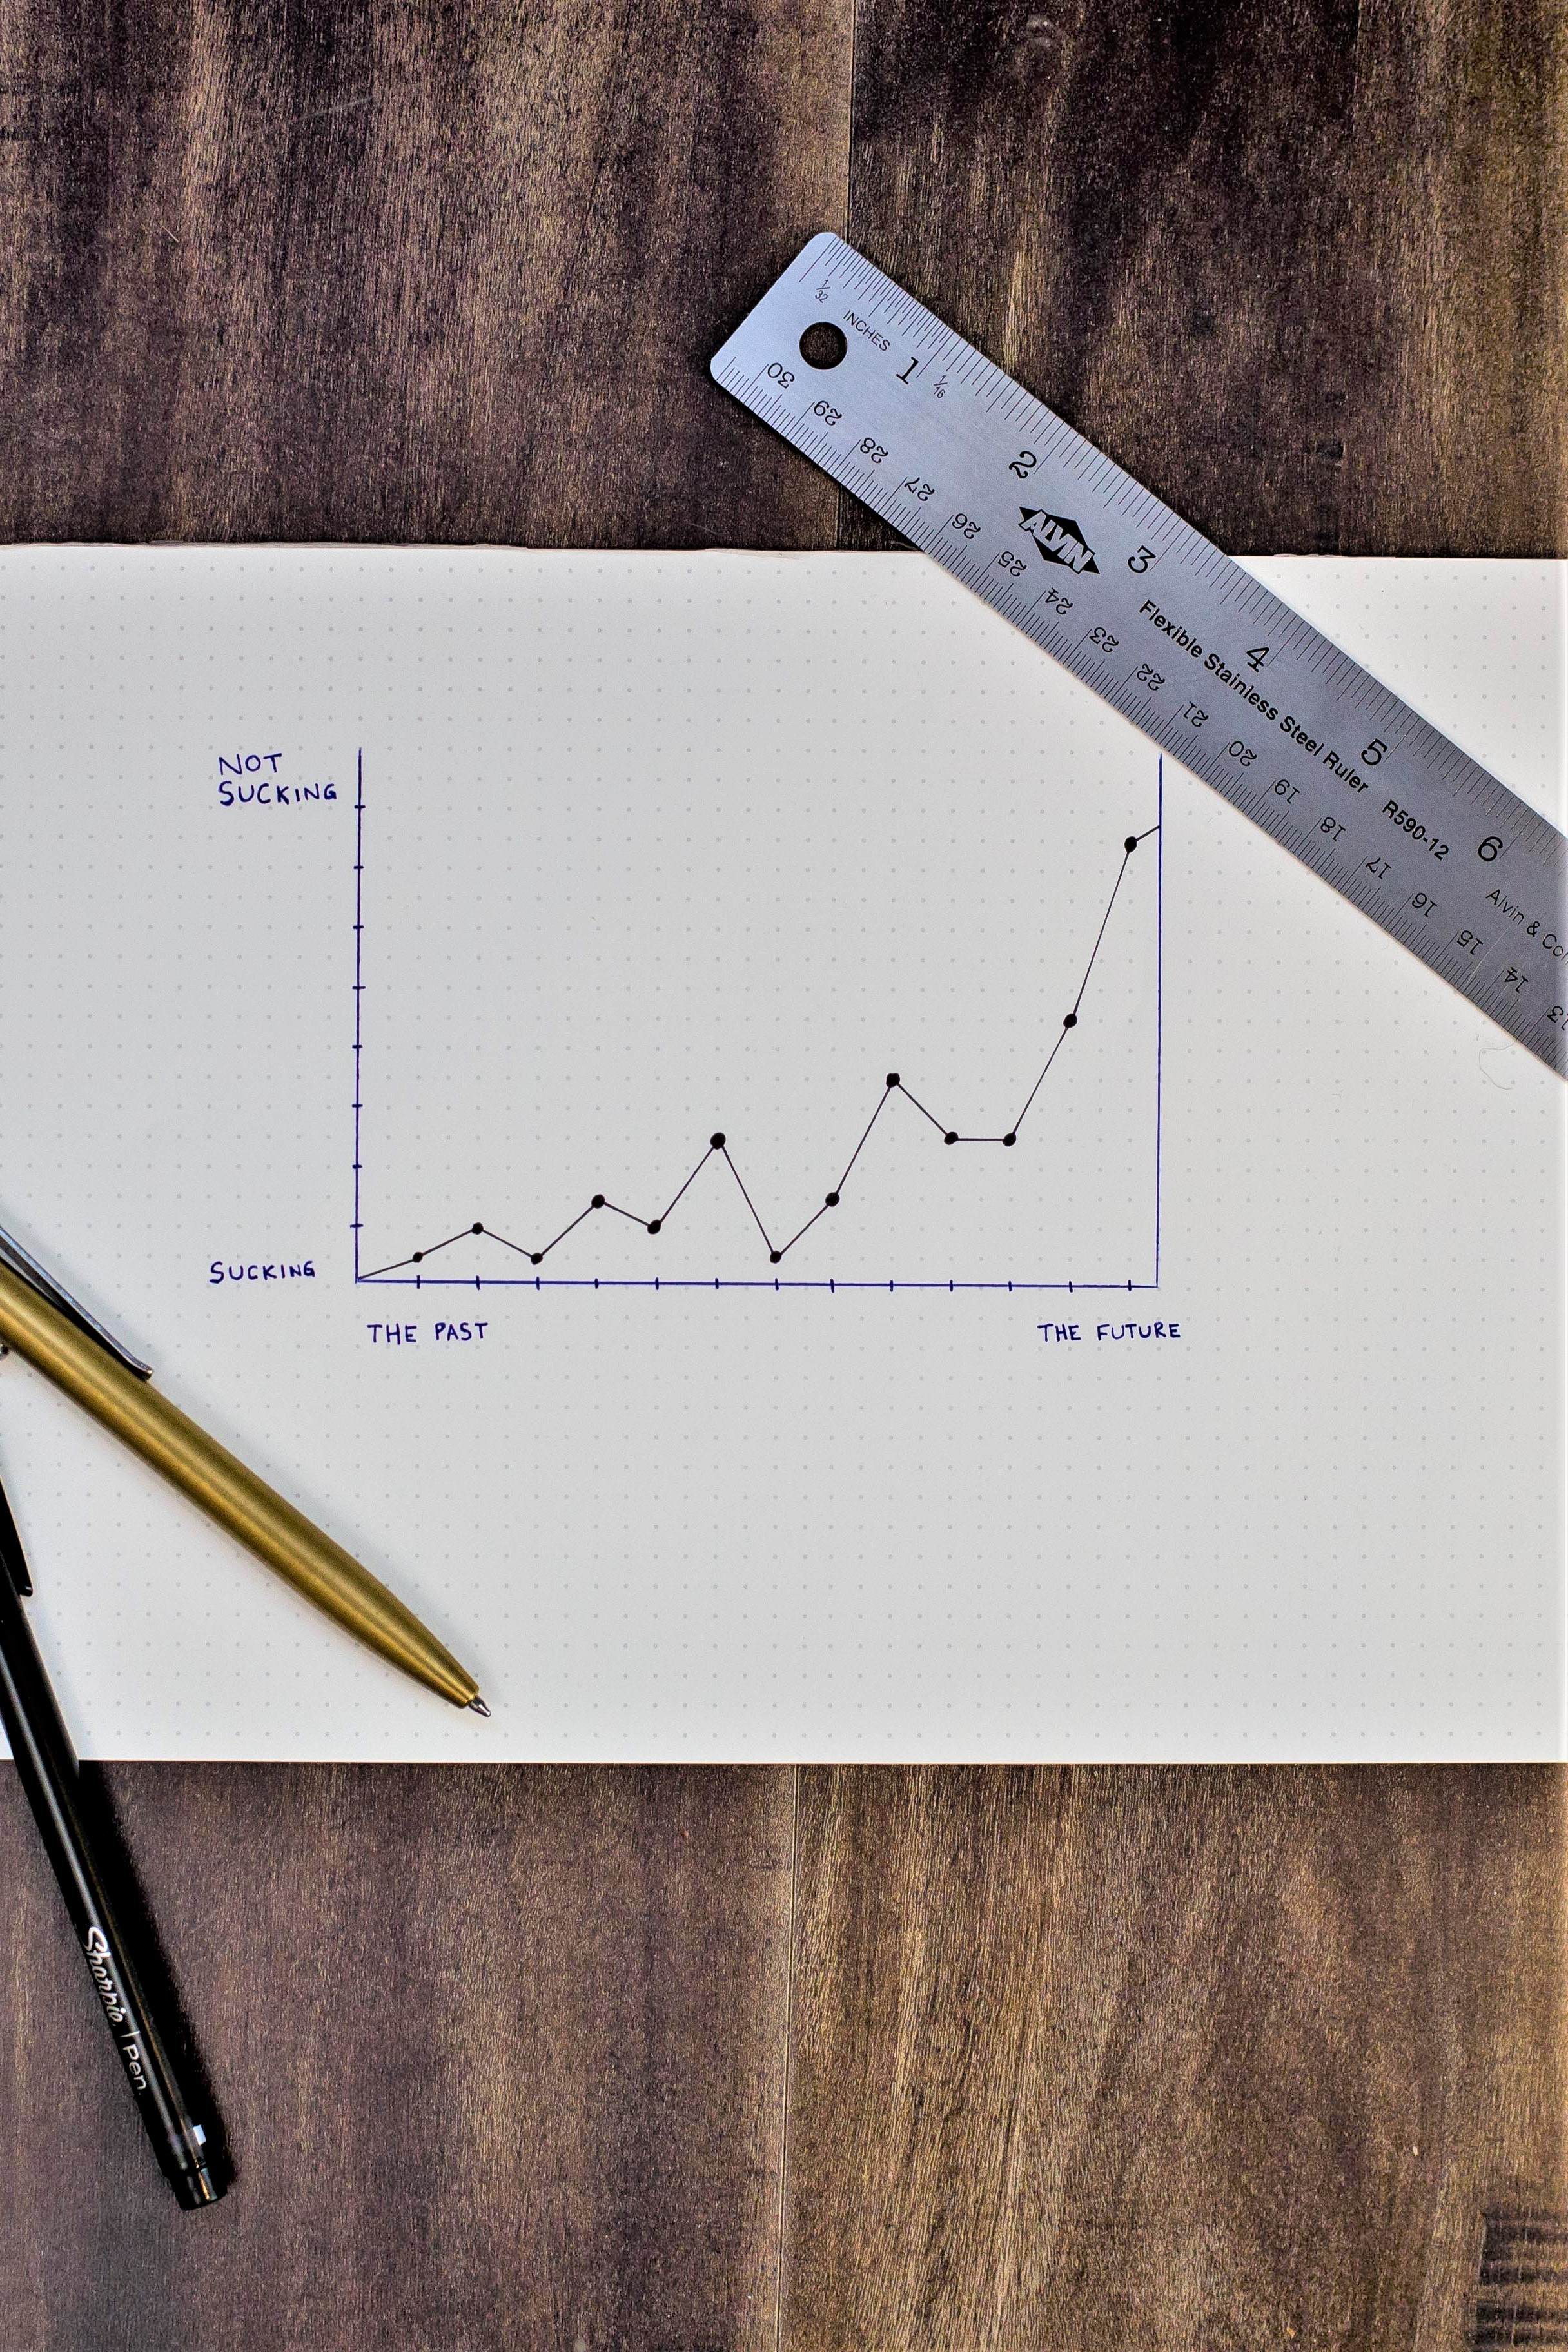
\includegraphics{images/cover.jpg}

\begin{center}
\includegraphics[width=0.25\linewidth]{logo} \end{center}

\hypertarget{introduction}{%
\chapter{Introduction}\label{introduction}}

This guide is an attempt to streamline and demystify the data analysis process.

By no means this is an ultimate guide, or I am a great source of knowledge, or I claim myself to be a statistician/ econometrician, but I am a strong proponent of learning by teaching, and doing. Hence, this is more like a learning experience for both you and me.

Since the beginning of the century, we have been bombarded with amazing advancements and inventions, especially in the field of statistics, information technology, computer science, or a new emerging filed - data science. However, I believe the downside of this introduction is that we use \textbf{big} and \textbf{trendy} words too often (i.e., big data, machine learning, deep learning).

It's all fun and exciting when I learned these new tools. But I have to admit that I hardly retain any of these new ideas. However, writing down from the beginning till the end of a data analysis process is the solution that I came up with. Accordingly, let's dive right in.

\begin{verbatim}
## Warning: package 'jpeg' was built under R version 4.0.5
\end{verbatim}

\begin{center}
\includegraphics[width=8.33in]{images/meme} \end{center}

\textbf{Some general recommendation}:

\begin{itemize}
\item
  The more you practice/habituate/condition, more line of codes that you write, more function that you memorize, I think the more you will like this journey.
\item
  Readers can follow this book several ways:

  \begin{itemize}
  \tightlist
  \item
    If you are interested in particular methods/tools, you can jump to that section by clicking the section name.
  \item
    If you want to follow a traditional path of data analysis, read the \protect\hyperlink{linear-regression}{Linear Regression} section.
  \item
    If you want to create your experiment and test your hypothesis, read the \protect\hyperlink{analysis-of-variance-anova}{Analysis of Variance (ANOVA)} section.
  \end{itemize}
\item
  Alternatively, if you rather see the application of models, and disregard any theory or underlying mechanisms, you can skip to summary and application portion of each section.
\item
  If you don't understand a part, search the title of that part of that part on Google, and read more into that subject. This is just a general guide.
\item
  If you want to customize your code beyond the ones provided in this book, run in the console \texttt{help(code)} or \texttt{?code}. For example, I want more information on \texttt{hist} function, I'll type in the console \texttt{?hist} or \texttt{help(hist)}.\\
\item
  Another way is that you can search on Google. Different people will use different packages to achieve the same result in R. Accordingly, if you want to create a histogram, search on Google \texttt{histogram\ in\ R}, then you should be able to find multiple ways to create histogram in R.
\end{itemize}

Information in this book are from various sources, but most of the content is based on several courses that I have taken formally. I'd like to give professors credit accordingly.

\begin{longtable}[]{@{}ll@{}}
\toprule
Course & Professor\tabularnewline
\midrule
\endhead
Data Analysis I & Erin M. Schliep\tabularnewline
Data Analysis II & Christopher Wikle\tabularnewline
Applied Econometric & Alyssa Carlson\tabularnewline
\bottomrule
\end{longtable}

\textbf{Tools of statistics}

\begin{itemize}
\tightlist
\item
  Probability Theory
\item
  Mathematical Analysis
\item
  Computer Science
\item
  Numerical Analysis
\item
  Database Management
\end{itemize}

\textbf{Setup Working Environment}

\begin{Shaded}
\begin{Highlighting}[]
\ControlFlowTok{if}\NormalTok{ (}\SpecialCharTok{!}\FunctionTok{require}\NormalTok{(}\StringTok{"pacman"}\NormalTok{))}
    \FunctionTok{install.packages}\NormalTok{(}\StringTok{"pacman"}\NormalTok{)}
\ControlFlowTok{if}\NormalTok{ (}\SpecialCharTok{!}\FunctionTok{require}\NormalTok{(}\StringTok{"devtools"}\NormalTok{))}
    \FunctionTok{install.packages}\NormalTok{(}\StringTok{"devtools"}\NormalTok{)}
\FunctionTok{library}\NormalTok{(}\StringTok{"pacman"}\NormalTok{)}
\FunctionTok{library}\NormalTok{(}\StringTok{"devtools"}\NormalTok{)}
\end{Highlighting}
\end{Shaded}

\hypertarget{prerequisites}{%
\chapter{Prerequisites}\label{prerequisites}}

This chapter is just a quick review of \protect\hyperlink{matrix-theory}{Matrix Theory} and \protect\hyperlink{probability-theory}{Probability Theory}

If you feel you do not need to brush up on these theories, you can jump right into \protect\hyperlink{descriptive-stat}{Descriptive Statistics}

\hypertarget{matrix-theory}{%
\section{Matrix Theory}\label{matrix-theory}}

\begin{equation}
\begin{split}
A=
\left[\begin{array}
{cc}
a_{11} & a_{12} \\
a_{21} & a_{22} \\
\end{array}
\right]
\end{split}
\end{equation}

\begin{equation}
\begin{split}
A' =
\left[\begin{array}
{cc}
a_{11} & a_{21} \\
a_{12} & a_{22} \\
\end{array}
\right]
\end{split}
\end{equation}

\[
\mathbf{(ABC)'=C'B'A'} \\
\mathbf{A(B+C)= AB + AC} \\
\mathbf{AB \neq BA} \\
\mathbf{(A')'=A} \\
\mathbf{(A+B)' = A' + B'} \\
\mathbf{(AB)' = B'A'} \\
\mathbf{(AB)^{-1}= B^{-1}A^{-1}} \\
\mathbf{A+B = B +A} \\
\mathbf{AA^{-1} = I }
\]

If A has an inverse, it is called \textbf{invertible.} If A is not invertible it is called \textbf{singular.}

\begin{equation}
\begin{split}
\mathbf{A} &= 
\left(\begin{array}
{ccc} 
a_{11} & a_{12} & a_{13} \\ 
a_{21} & a_{22} & a_{23} \\ 
\end{array}\right)
\left(\begin{array}
{ccc}
b_{11} & b_{12} & b_{13} \\
b_{21} & b_{22} & b_{23} \\
b_{31} & b_{32} & b_{33} \\
\end{array}\right) \\
&= 
\left(\begin{array}
{ccc}
a_{11}b_{11}+a_{12}b_{21}+a_{13}b_{31} & \sum_{i=1}^{3}a_{1i}b_{i2} &  \sum_{i=1}^{3}a_{1i}b_{i3} \\
\sum_{i=1}^{3}a_{2i}b_{i1} & \sum_{i=1}^{3}a_{2i}b_{i2} & \sum_{i=1}^{3}a_{2i}b_{i3} \\
\end{array}\right) 
\end{split}
\end{equation}

Let \(\mathbf{a}\) be a 3 x 1 vector, then the quadratic form is

\[
\mathbf{a'Ba} = \sum_{i=1}^{3}\sum_{i=1}^{3}a_i b_{ij} a_{j}
\]

\textbf{Length of a vector}\\
Let \(\mathbf{a}\) be a vector, \(||\mathbf{a}||\) (the 2-norm of the vector) is the length of vector \(\mathbf{a}\), is the square root of the inner product of the vector with itself:

\[
||\mathbf{a}|| = \sqrt{\mathbf{a'a}}
\]

\hypertarget{rank}{%
\subsection{Rank}\label{rank}}

\begin{itemize}
\tightlist
\item
  Dimension of space spanned by its columns (or its rows).\\
\item
  Number of linearly independent columns/rows
\end{itemize}

For a n x k matrix \textbf{A} and k x k matrix \textbf{B}

\begin{itemize}
\tightlist
\item
  \(rank(A)\leq min(n,k)\)
\item
  \(rank(A) = rank(A') = rank(A'A)=rank(AA')\)
\item
  \(rank(AB)=min(rank(A),rank(B))\)
\item
  \textbf{B} is invertible if and only if rank(B) = k (non-singular)
\end{itemize}

\hypertarget{inverse}{%
\subsection{Inverse}\label{inverse}}

In scalar, a = 0 then 1/a does not exist. In matrix, a matrix is invertible when it's a non-zero matrix.

A non-singular square matrix A is invertible if there exists a non-singular square matrix B such that, \[AB=I\] Then \(A^{-1}=B\). For a 2x2 matrix,

\[
A =
\left(\begin{array}{cc}
a & b \\
c & d \\
\end{array}
\right)
\]

\[
A^{-1}=
\frac{1}{ad-bc}
\left(\begin{array}{cc}
d & -b \\
-c & a \\
\end{array}
\right)
\]

For the partition matrix,

\begin{equation}
\begin{split}
\left[\begin{array}
{cc}
A & B \\
C & D \\
\end{array}
\right]^{-1}
 =
\left[\begin{array}
{cc}
\mathbf{(A-BD^{-1}C)^{-1}} & \mathbf{-(A-BD^{-1}C)^{-1}BD^-1}\\
\mathbf{-DC(A-BD^{-1}C)^{-1}} & \mathbf{D^{-1}+D^{-1}C(A-BD^{-1}C)^{-1}BD^{-1}}\ \\
\end{array}
\right]
\end{split}
\end{equation}

Properties for a non-singular square matrix

\begin{itemize}
\tightlist
\item
  \(\mathbf{A^{-1}}=A\)
\item
  for a non-zero scalar b, \(\mathbf{(bA)^{-1}=b^{-1}A^{-1}}\)
\item
  for a matrix B, \(\mathbf(BA)^{-1}=B^{-1}A^{-1}\) only if B is non-singular
\item
  \(\mathbf{(A^{-1})'=(A')^{-1}}\)
\item
  Never notate \(\mathbf{1/A}\)
\end{itemize}

\hypertarget{definiteness}{%
\subsection{Definiteness}\label{definiteness}}

A symmetric square k x k matrix, \(\mathbf{A}\), is Positive Semi-Definite if for any non-zero k x 1 vector \(\mathbf{x}\), \[\mathbf{x'Ax \geq 0 }\]

A symmetric square k x k matrix, \(\mathbf{A}\), is Negative Semi-Definite if for any non-zero k x 1 vector \(\mathbf{x}\) \[\mathbf{x'Ax \leq 0 }\]

\(\mathbf{A}\) is indefinite if it is neither positive semi-definite or negative semi-definite.

The identity matrix is positive definite

\textbf{Example} Let \(\mathbf{x} =(x_1 x_2)'\), then for a 2 x 2 identity matrix,

\begin{equation}
\begin{split}
\mathbf{x'Ix} 
&= (x_1 x_2) 
\left(\begin{array}
{cc}
1 & 0 \\
0 & 1 \\
\end{array}
\right)
\left(\begin{array}{c}
x_1 \\
x_2 \\
\end{array}
\right) \\
&=
(x_1 x_2)
\left(\begin{array}
{c}
x_1 \\
x_2 \\
\end{array}
\right) \\
&=
x_1^2 + x_2^2 >0
\end{split}
\end{equation}

Definiteness gives us the ability to compare matrices \(\mathbf{A-B}\) is PSD This property also helps us show efficiency (which variance covariance matrix of one estimator is smaller than another)

Properties

\begin{itemize}
\tightlist
\item
  any variance matrix is PSD
\item
  a matrix \(\mathbf{A}\) is PSD if and only if there exists a matrix \(\mathbf{B}\) such that \(\mathbf{A=B'B}\)
\item
  if \(\mathbf{A}\) is PSD, then \(\mathbf{B'AB}\) is PSD
\item
  if A and C are non-singular, then A-C is PSD if and only if \(\mathbf{C^{-1}-A^{-1}}\)
\item
  if A is PD (ND) then \(A^{-1}\) is PD (ND)
\end{itemize}

\textbf{Note}

\begin{itemize}
\tightlist
\item
  Indefinite A is neither PSD nor NSD. There is no comparable concept in scalar.
\item
  If a square matrix is PSD and invertible then it is PD
\end{itemize}

Example:

\begin{enumerate}
\def\labelenumi{\arabic{enumi}.}
\tightlist
\item
  Invertible / Indefinite
\end{enumerate}

\[
\left[
\begin{array}
{cc}
-1 & 0 \\
0 & 10 \\
\end{array}
\right]
\]

\begin{enumerate}
\def\labelenumi{\arabic{enumi}.}
\setcounter{enumi}{1}
\tightlist
\item
  Non-invertible/ Indefinite
\end{enumerate}

\[
\left[
\begin{array}
{cc}
0 & 1 \\
0 & 0 \\
\end{array}
\right]
\]

\begin{enumerate}
\def\labelenumi{\arabic{enumi}.}
\setcounter{enumi}{2}
\tightlist
\item
  Invertible / PSD
\end{enumerate}

\[
\left[
\begin{array}
{cc}
1 & 0 \\
0 & 1 \\
\end{array}
\right]
\]

\begin{enumerate}
\def\labelenumi{\arabic{enumi}.}
\setcounter{enumi}{3}
\tightlist
\item
  Non-Invertible / PSD
\end{enumerate}

\[
\left[
\begin{array}
{cc}
0 & 0 \\
0 & 1 \\
\end{array}
\right]
\]

\hypertarget{matrix-calculus}{%
\subsection{Matrix Calculus}\label{matrix-calculus}}

\(y=f(x_1,x_2,...,x_k)=f(x)\) where x is a 1 x k row vector. The Gradient (first order derivative with respect to a vector) is,

\[
\frac{\partial{f(x)}}{\partial{x}}=
\left(\begin{array}{c}
\frac{\partial{f(x)}}{\partial{x_1}} \\
\frac{\partial{f(x)}}{\partial{x_2}} \\
... \\
\frac{\partial{f(x)}}{\partial{x_k}}
\end{array}
\right)
\]

The \textbf{Hessian} (second order derivative with respect to a vector) is,

\[
\frac{\partial^2{f(x)}}{\partial{x}\partial{x'}}=
\left(\begin{array}
{cccc}
\frac{\partial^2{f(x)}}{\partial{x_1}\partial{x_1}} & \frac{\partial^2{f(x)}}{\partial{x_1}\partial{x_2}} & ... & \frac{\partial^2{f(x)}}{\partial{x_1}\partial{x_k}} \\
\frac{\partial^2{f(x)}}{\partial{x_1}\partial{x_2}} & \frac{\partial^2{f(x)}}{\partial{x_2}\partial{x_2}} & ... & \frac{\partial^2{f(x)}}{\partial{x_2}\partial{x_k}} \\
... & ...& & ...\\
\frac{\partial^2{f(x)}}{\partial{x_k}\partial{x_1}} & \frac{\partial^2{f(x)}}{\partial{x_k}\partial{x_2}} & ... & \frac{\partial^2{f(x)}}{\partial{x_k}\partial{x_k}}
\end{array}
\right)
\]

Define the derivative of \(f(\mathbf{X})\) with respect to \(\mathbf{X}_{(n \times p)}\) as the matrix

\[
\frac{\partial f(\mathbf{X})}{\partial \mathbf{X}} = (\frac{\partial f(\mathbf{X})}{\partial x_{ij}})
\]

Define \(\mathbf{a}\) to be a vector and \(\mathbf{A}\) to be a matrix which does not depend upon \(\mathbf{y}\). Then

\[
\frac{\partial \mathbf{a'y}}{\partial \mathbf{y}} = \mathbf{a}
\]

\[
\frac{\partial \mathbf{y'y}}{\partial \mathbf{y}} = 2\mathbf{y}
\]

\[
\frac{\partial \mathbf{y'Ay}}{\partial \mathbf{y}} = \mathbf{(A + A')y}
\]

If \(\mathbf{X}\) is a symmetric matrix then

\[
\frac{\partial |\mathbf{X}|}{\partial x_{ij}} = 
\begin{cases}
X_{ii}, i = j \\
X_ij, i \neq j
\end{cases}
\]
where \(X_{ij}\) is the (i,j)th cofactor of \(\mathbf{X}\)

If \(\mathbf{X}\) is symmetric and \(\mathbf{A}\) is a matrix which does not depend upon \(\mathbf{X}\) then

\[
\frac{\partial tr \mathbf{XA}}{\partial \mathbf{X}} = \mathbf{A} + \mathbf{A}' - diag(\mathbf{A})
\]

If \(\mathbf{X}\) is symmetric and we let \(\mathbf{J}_{ij}\) be a matrix which has a 1 in the (i,j)th position and 0s elsewhere, then

\[
\frac{\partial \mathbf{X}6{-1}}{\partial x_{ij}} = 
\begin{cases}
- \mathbf{X}^{-1}\mathbf{J}_{ii} \mathbf{X}^{-1} , i = j \\
- \mathbf{X}^{-1}(\mathbf{J}_{ij} + \mathbf{J}_{ji}) \mathbf{X}^{-1} , i \neq j
\end{cases}
\]

\hypertarget{optimization}{%
\subsection{Optimization}\label{optimization}}

\begin{longtable}[]{@{}lcc@{}}
\toprule
\begin{minipage}[b]{(\columnwidth - 2\tabcolsep) * \real{0.19}}\raggedright
\strut
\end{minipage} & \begin{minipage}[b]{(\columnwidth - 2\tabcolsep) * \real{0.27}}\centering
\textbf{Scalar Optimization}\strut
\end{minipage} & \begin{minipage}[b]{(\columnwidth - 2\tabcolsep) * \real{0.54}}\centering
\textbf{Vector Optimization}\strut
\end{minipage}\tabularnewline
\midrule
\endhead
\begin{minipage}[t]{(\columnwidth - 2\tabcolsep) * \real{0.19}}\raggedright
First Order Condition\strut
\end{minipage} & \begin{minipage}[t]{(\columnwidth - 2\tabcolsep) * \real{0.27}}\centering
\[\frac{\partial{f(x_0)}}{\partial{x}}=0\]\strut
\end{minipage} & \begin{minipage}[t]{(\columnwidth - 2\tabcolsep) * \real{0.54}}\centering
\[\frac{\partial{f(x_0)}}{\partial{x}}=\left(\begin{array}{c}0 \\ .\\ .\\ .\\ 0\end{array}\right)\]\strut
\end{minipage}\tabularnewline
\begin{minipage}[t]{(\columnwidth - 2\tabcolsep) * \real{0.19}}\raggedright
Second Order Condition ~

\textbf{Convex} \(\rightarrow\) \textbf{Min}\strut
\end{minipage} & \begin{minipage}[t]{(\columnwidth - 2\tabcolsep) * \real{0.27}}\centering
\[\frac{\partial^2{f(x_0)}}{\partial{x^2}} > 0\]\strut
\end{minipage} & \begin{minipage}[t]{(\columnwidth - 2\tabcolsep) * \real{0.54}}\centering
\[\frac{\partial^2{f(x_0)}}{\partial{xx'}}>0\]\strut
\end{minipage}\tabularnewline
\begin{minipage}[t]{(\columnwidth - 2\tabcolsep) * \real{0.19}}\raggedright
\textbf{Concave} \(\rightarrow\) \textbf{Max}\strut
\end{minipage} & \begin{minipage}[t]{(\columnwidth - 2\tabcolsep) * \real{0.27}}\centering
\[\frac{\partial^2{f(x_0)}}{\partial{x^2}} < 0\]\strut
\end{minipage} & \begin{minipage}[t]{(\columnwidth - 2\tabcolsep) * \real{0.54}}\centering
\[\frac{\partial^2{f(x_0)}}{\partial{xx'}}<0\]\strut
\end{minipage}\tabularnewline
\bottomrule
\end{longtable}

\hypertarget{probability-theory}{%
\section{Probability Theory}\label{probability-theory}}

\hypertarget{axiom-and-theorems-of-probability}{%
\subsection{Axiom and Theorems of Probability}\label{axiom-and-theorems-of-probability}}

\begin{enumerate}
\def\labelenumi{\arabic{enumi}.}
\tightlist
\item
  Let S denote a sample space of an experiment P{[}S{]}=1
\item
  \(P[A] \ge 0\) for every event A
\item
  Let \(A_1,A_2,A_3,...\) be a finite or an infinite collection of mutually exclusive events. Then \(P[A_1\cup A_2 \cup A_3 ...]=P[A_1]+P[A_2]+P[A_3]+...\)
\item
  \(P[\emptyset]=0\)
\item
  \(P[A']=1-P[A]\)
\item
  \(P[A_1 \cup A_2] = P[A_1] + P[A_2] - P[A_1 \cap A_2]\)
\end{enumerate}

\textbf{Conditional Probability}

\[
P[A|B]=\frac{A \cap B}{P[B]}
\]

\textbf{Independent Events} Two events A and B are independent if and only if:

\begin{enumerate}
\def\labelenumi{\arabic{enumi}.}
\tightlist
\item
  \(P[A\cap B]=P[A]P[B]\)
\item
  \(P[A|B]=P[A]\)
\item
  \(P[B|A]=P[B]\)
\end{enumerate}

A finite collection of events \(A_1, A_2, ..., A_n\) is independent if and only if any subcollection is independent.

\textbf{Multiplication Rule} \(P[A \cap B] = P[A|B]P[B] = P[B|A]P[A]\)

\textbf{Bayes' Theorem} Let \(A_1, A_2, ..., A_n\) be a collection of mutually exclusive events whose union is S.\\
Let b be an event such that \(P[B]\neq0\)\\
Then for any of the events \(A_j\), j = 1,2,\ldots,n

\[
P[A_|B]=\frac{P[B|A_j]P[A_j]}{\sum_{i=1}^{n}P[B|A_j]P[A_i]}
\]

\textbf{Jensen's Inequality}

\begin{itemize}
\tightlist
\item
  If g(x) is convex \(E(g(X)) \ge g(E(X))\)
\item
  If g(x) is concave \(E(g(X)) \le g(E(X))\)
\end{itemize}

\hypertarget{law-of-iterated-expectations}{%
\subsubsection{Law of Iterated Expectations}\label{law-of-iterated-expectations}}

\(E(Y)=E(E(Y|X))\)

\hypertarget{correlation-and-independence}{%
\subsubsection{Correlation and Independence}\label{correlation-and-independence}}

\textbf{Independence}

\begin{itemize}
\tightlist
\item
  \(f(x,y)=f_X(x)f_Y(y)\)
\item
  \(f_{Y|X}(y|x)=f_Y(y)\) and \(f_{X|Y}(x|y)=f_X(x)\)
\item
  \(E(g_1(X)g_2(Y))=E(g_1(X))E(g_2(Y))\)
\end{itemize}

\textbf{Mean Independence} (implied by independence)

\begin{itemize}
\tightlist
\item
  Y is mean independent of X if and only if \(E(Y|X)=E(Y)\)
\item
  \(E(Xg(Y))=E(X)E(g(Y))\)
\end{itemize}

\textbf{Uncorrelated} (implied by independence and mean independence)

\begin{itemize}
\tightlist
\item
  \(Cov(X,Y)=0\)
\item
  \(Var(X+Y)=Var(X) + Var(Y)\)
\item
  \(E(XY)=E(X)E(Y)\)
\end{itemize}

\[
Strongest \\
\downarrow \\
Independence \\
\downarrow \\
Mean Independence \\
\downarrow \\
Uncorrelated \\ 
\downarrow \\
Weakest\\
\]

\hypertarget{central-limit-theorem}{%
\subsection{Central Limit Theorem}\label{central-limit-theorem}}

Let \(X_1, X_2,...,X_n\) be a random sample of size n from a distribution (not necessarily normal) X with mean \(\mu\) and variance \(\sigma^2\). then for large n (\(n \ge 25\)),

\begin{enumerate}
\def\labelenumi{\arabic{enumi}.}
\item
  \(\bar{X}\) is approximately normal with with mean \(\mu_{\bar{X}}=\mu\) and variance \(\sigma^2_{\bar{X}} = Var(\bar{X})= \frac{\sigma^2}{n}\)\\
\item
  \(\hat{p}\)is approximately normal with \(\mu_{\hat{p}} = p, \sigma^2_{\hat{p}} = \frac{p(1-p)}{n}\)
\item
  \(\hat{p_1} - \hat{p_2}\) is approximately normal with \(\mu_{\hat{p_1} - \hat{p_2}} = p_1 - p_2, \sigma^2_{\hat{p_1} - \hat{p_2}}=\frac{p_1(1-p)}{n_1} + \frac{p_2(1-p)}{n_2}\)
\item
  \(\bar{X_1} - \bar{X_2}\) is approximately normal with \(\mu_{\bar{X_1} - \bar{X_2}} = \mu_1 - \mu_2, \sigma^2_{\bar{X_1} - \bar{X_2}} = \frac{\sigma^2_1}{n_1}+\frac{\sigma^2_2}{n_2}\)
\item
  The following random variables are approximately standard normal:\\

  \begin{itemize}
  \tightlist
  \item
    \(\frac{\bar{X}-\mu}{\sigma/\sqrt{n}}\)\\
  \item
    \(\frac{\hat{p}-p}{\sqrt{\frac{p(1-p)}{n}}}\)\\
  \item
    \(\frac{(\hat{p_1}-\hat{p_2})-(p_1-p_2)}{\sqrt{\frac{p_1(1-p_1)}{n_1}-\frac{p_2(1-p_2)}{n_2}}}\)\\
  \item
    \(\frac{(\bar{X_1}-\bar{X_2})-(\mu_1-\mu_2)}{\sqrt{\frac{\sigma^2_1}{n_1}-\frac{\sigma^2_2}{n_2}}}\)
  \end{itemize}
\end{enumerate}

If \(\{x_i\}_{i=1}^{n}\) is an iid random sample from a probability distribution with finite mean \(\mu\) and finite variance \(\sigma^2\) then the sample mean \(\bar{x}=n^{-1}\sum_{i=1}^{n}x_i\) scaled by \(\sqrt{n}\) has the following limiting distribution

\[
\sqrt{n}(\bar{x}-\mu) \to^d N(0,\sigma^2)
\]

or if we were to standardize the sample mean,

\[
\frac{\sqrt{n}(\bar{x}-\mu)}{\sigma} \to^d N(0,1)
\]

\begin{itemize}
\tightlist
\item
  holds for most random sample from any distribution (continuous, discrete, unknown).\\
\item
  extends to multivariate case: random sample of a random vector converges to a multivariate normal.\\
\item
  Variance from the limiting distribution is the asymptotic variance (Avar)
\end{itemize}

\[
Avar(\sqrt{n}(\bar{x}-\mu)) = \sigma^2 \\
\lim_{n \to \infty} Var(\sqrt{n}(\bar{x}-\mu)) = \sigma^2 \\
Avar(.) \neq lim_{n \to \infty} Var(.)
\]

\hypertarget{random-variable}{%
\subsection{Random variable}\label{random-variable}}

\begin{longtable}[]{@{}lll@{}}
\toprule
\begin{minipage}[b]{(\columnwidth - 2\tabcolsep) * \real{0.22}}\raggedright
\strut
\end{minipage} & \begin{minipage}[b]{(\columnwidth - 2\tabcolsep) * \real{0.31}}\raggedright
Discrete Variable\strut
\end{minipage} & \begin{minipage}[b]{(\columnwidth - 2\tabcolsep) * \real{0.47}}\raggedright
Continuous Variable\strut
\end{minipage}\tabularnewline
\midrule
\endhead
\begin{minipage}[t]{(\columnwidth - 2\tabcolsep) * \real{0.22}}\raggedright
\textbf{Definition}\strut
\end{minipage} & \begin{minipage}[t]{(\columnwidth - 2\tabcolsep) * \real{0.31}}\raggedright
A random variable is discrete if it can assume at most a finite or countably infinite number of possible values\strut
\end{minipage} & \begin{minipage}[t]{(\columnwidth - 2\tabcolsep) * \real{0.47}}\raggedright
A random variable is continuous if it can assume any value in some interval or intervals of real numbers and the probability that it assumes any specific value is 0\strut
\end{minipage}\tabularnewline
\begin{minipage}[t]{(\columnwidth - 2\tabcolsep) * \real{0.22}}\raggedright
\textbf{Density Function}\strut
\end{minipage} & \begin{minipage}[t]{(\columnwidth - 2\tabcolsep) * \real{0.31}}\raggedright
A function f is called a density for X if: (1) \(f(x) \ge 0\) (2) \(\sum_{all~x}f(x)=1\) (3) \(f(x)=P(X=x)\) for x real\strut
\end{minipage} & \begin{minipage}[t]{(\columnwidth - 2\tabcolsep) * \real{0.47}}\raggedright
A function f is called a density for X if: (1) \(f(x) \ge 0\) for x real (2) \(\int_{-\infty}^{\infty} f(x) \; dx=1\) (3) \(P[a \le X \le] =\int_{a}^{b} f(x) \; dx\) for a and b real\strut
\end{minipage}\tabularnewline
\begin{minipage}[t]{(\columnwidth - 2\tabcolsep) * \real{0.22}}\raggedright
\textbf{Cumulative Distribution Function} for x real\strut
\end{minipage} & \begin{minipage}[t]{(\columnwidth - 2\tabcolsep) * \real{0.31}}\raggedright
\(F(x)=P[X \le x]\)\strut
\end{minipage} & \begin{minipage}[t]{(\columnwidth - 2\tabcolsep) * \real{0.47}}\raggedright
\(F(x)=P[X \le x]=\int_{-\infty}^{\infty}f(t)dt\)\strut
\end{minipage}\tabularnewline
\begin{minipage}[t]{(\columnwidth - 2\tabcolsep) * \real{0.22}}\raggedright
\(E[H(X)]\)\strut
\end{minipage} & \begin{minipage}[t]{(\columnwidth - 2\tabcolsep) * \real{0.31}}\raggedright
\(\sum_{all ~x}H(x)f(x)\)\strut
\end{minipage} & \begin{minipage}[t]{(\columnwidth - 2\tabcolsep) * \real{0.47}}\raggedright
\(\int_{-\infty}^{\infty}H(x)f(x)\)\strut
\end{minipage}\tabularnewline
\begin{minipage}[t]{(\columnwidth - 2\tabcolsep) * \real{0.22}}\raggedright
\(\mu=E[X]\)\strut
\end{minipage} & \begin{minipage}[t]{(\columnwidth - 2\tabcolsep) * \real{0.31}}\raggedright
\(\sum_{all ~ x}xf(x)\)\strut
\end{minipage} & \begin{minipage}[t]{(\columnwidth - 2\tabcolsep) * \real{0.47}}\raggedright
\(\int_{-\infty}^{\infty}xf(x)\)\strut
\end{minipage}\tabularnewline
\begin{minipage}[t]{(\columnwidth - 2\tabcolsep) * \real{0.22}}\raggedright
\textbf{Ordinary Moments} the kth ordinary moment for variable X is defined as: \(E[X^k]\)\strut
\end{minipage} & \begin{minipage}[t]{(\columnwidth - 2\tabcolsep) * \real{0.31}}\raggedright
\(\sum_{all ~ x \in X}(x^kf(x))\)\strut
\end{minipage} & \begin{minipage}[t]{(\columnwidth - 2\tabcolsep) * \real{0.47}}\raggedright
\(\int_{-\infty}^{\infty}(x^kf(x))\)\strut
\end{minipage}\tabularnewline
\begin{minipage}[t]{(\columnwidth - 2\tabcolsep) * \real{0.22}}\raggedright
\textbf{Moment generating function (mgf)} \(m_X(t)=E[e^{tX}]\)\strut
\end{minipage} & \begin{minipage}[t]{(\columnwidth - 2\tabcolsep) * \real{0.31}}\raggedright
\(\sum_{all ~ x \in X}(e^{tx}f(x))\)\strut
\end{minipage} & \begin{minipage}[t]{(\columnwidth - 2\tabcolsep) * \real{0.47}}\raggedright
\(\int_{-\infty}^{\infty}(e^{tx}f(x)dx)\)\strut
\end{minipage}\tabularnewline
\bottomrule
\end{longtable}

Expected Value Properties:

\begin{itemize}
\tightlist
\item
  E{[}c{]} = c for any constant c
\item
  E{[}cX{]} = cE{[}X{]} for any constant c
\item
  E{[}X+Y{]} = E{[}X{]} = E{[}Y{]}
\item
  E{[}XY{]} = E{[}X{]}.E{[}Y{]} (if X and Y are independent)
\end{itemize}

Expected Variance Properties:

\begin{itemize}
\tightlist
\item
  \(Var(c) = 0\) for any constant c
\item
  \(Var(cX) = c^2Var(X)\) for any constant c
\item
  \(Var(X) \ge 0\)
\item
  \(Var(X) = E(X^2) - (E(X))^2\)
\item
  \(Var(X+c)=Var(X)\)
\item
  \(Var (X+Y) = Var(X) + Var(Y)\) (if X and Y are independent)
\end{itemize}

Standard deviation \(\sigma=\sqrt(\sigma^2)=\sqrt(Var X)\)

Suppose \(y_1,...,y_p\) are possibly correlated random variables with means \(\mu_1,...,\mu_p\). then

\[
\mathbf{y} = (y_1,...,y_p)'  \\
E(\mathbf{y}) = (\mu_1,...,\mu_p)' = \mathbf{\mu}
\]

Let \(\sigma_{ij} = cov(y_i,y_j)\) for \(i,j = 1,..,p\).

Define

\[
\mathbf{\Sigma} = (\sigma_{ij}) = 
\left(\begin{array}
{rrrr}
\sigma_{11} & \sigma_{12} & ... & \sigma_{1p} \\
\sigma_{21} & \sigma_{22} & ... & \sigma_{2p} \\
. & . & . & . \\
\sigma_{p1} & \sigma_{p2} & ... & \sigma_{pp}\\
\end{array}\right)
\]

Hence, \(\mathbf{\Sigma}\) is the variance-covariance or dispersion matrix. And \(\mathbf{\Sigma}\) is symmetric with \((p+1)p/2\) unique parameters.

Alternatively, let \(u_{p \times 1}\) and \(v_{v \times 1}\) be random vectors with means \(\mathbf{\mu_u}\) and \(\mathbf{\mu_v}\). then

\[
\mathbf{\Sigma_{uv}} = cov(\mathbf{u,v}) = E[\mathbf{(u-\mu_u)(v-\mu_v)'}]
\]

\(\Sigma_{uv} \neq \Sigma_{vu}\) (but \(\Sigma_{uv} = \Sigma_{vu}'\))

Properties of Covariance Matrices

\begin{enumerate}
\def\labelenumi{\arabic{enumi}.}
\tightlist
\item
  Symmetric: \(\mathbf{\Sigma' = \Sigma}\)\\
\item
  Eigendecomposition (spectral decomposition,symmetric decomposition): \(\mathbf{\Sigma = \Phi \Lambda \Phi}\), where \(\mathbf{\Phi}\) is a matrix of eigenvectors such that \(\mathbf{\Phi \Phi' = I}\) (orthonormal), and \(\mathbf{\Lambda}\) is a diagonal matrix with eigenvalues \((\lambda_1,...,\lambda_p)\) on the diagonal.\\
\item
  Non-negative definite, \(\mathbf{a \Sigma a} \ge 0\) for any \(\mathbf{a} \in R^p\). Equivalently, the eigenvalues of \(\mathbf{\Sigma}\), \(\lambda_1 \ge ... \ge \lambda_p \ge 0\)\\
\item
  \(|\mathbf{\Sigma}| = \lambda_1,...\lambda_p \ge 0\) (generalized variance)\\
\item
  \(trace(\mathbf{\Sigma})= tr(\mathbf{\Sigma}) = \lambda_1 +... + \lambda_p = \sigma_{11}+...+ \sigma_{pp}\)= sum of variances (total variance)
\end{enumerate}

Note: \(\mathbf{\Sigma}\) is usually required to be positive definite. This implies that all eigenvalues are positive, and \(\mathbf{\Sigma}\) has an inverse \(\mathbf{\Sigma}^{-1}\), such that \(\mathbf{\Sigma}^{-1}\mathbf{\Sigma}= \mathbf{I}_{p \times p} = \mathbf{\Sigma}\mathbf{\Sigma}^{-1}\)

\textbf{Correlation Matrices}

Define the correlation \(\rho_{ij}\) and the correlation matrix by

\[
\rho_{ij} = \frac{\sigma_{ij}}{\sqrt{\sigma_{ii} \sigma_{jj}}}
\]

\[
\mathbf{R} = \left(
\begin{array}
{cccc}
\rho_{11} & \rho_{12} & ... & \rho_{1p} \\
\rho_{21} & \rho_{22} & ... & \rho_{2p} \\
. & . & . & . \\
\rho_{p1} & \rho_{p2} & ... & \rho_{pp}\\
\end{array}
\right)
\]

where \(\rho_{ii}=1\) for all i.

Let x and y be random vectors with means \(\mu_x\) and \(\mu_y\) and variance-covariance matrices \(\Sigma_x\) and \(\Sigma_y\). Let \(\mathbf{A}\) and \(\mathbf{B}\) be matrices of constants and c and d be vectors of constants. Then,

\begin{itemize}
\tightlist
\item
  \(E(\mathbf{Ay+c}) = \mathbf{A \mu_y} +c\)
\item
  \(var(\mathbf{Ay +c}) = \mathbf{A}var(\mathbf{y}) \mathbf{A}' = \mathbf{A \Sigma_y A'}\)
\item
  \(cov(\mathbf{Ay + c,By+d} = \mathbf{A \Sigma_y B'}\)
\end{itemize}

\hypertarget{moment-generating-function}{%
\subsection{Moment generating function}\label{moment-generating-function}}

Moment generating function properties:

\begin{enumerate}
\def\labelenumi{(\alph{enumi})}
\tightlist
\item
  \(\frac{d^k(m_X(t))}{dt^k}|_{t=0}=E[X^k]\)\\
\item
  \(\mu=E[X]=m_X'(0)\)\\
\item
  \(E[X^2]=m_X''(0)\)
\end{enumerate}

\textbf{mgf Theorems}

Let \(X_1,X_2,...X_n,Y\) be random variables with moment-generating functions \(m_{X_1}(t),m_{X_2}(t),...,m_{X_n}(t),m_{Y}(t)\)

\begin{enumerate}
\def\labelenumi{\arabic{enumi}.}
\tightlist
\item
  If \(m_{X_1}(t)=m_{X_2}(t)\) for all t in some open interval about 0, then \(X_1\) and \(X_2\) have the same distribution
\item
  If \(Y = \alpha + \beta X_1\), then \(m_{Y}(t)= e^{\alpha t}m_{X_1}(\beta t)\)
\item
  If \(X_1,X_2,...X_n\) are independent and \(Y = \alpha_0 + \alpha_1 X_1 + \alpha_2 X_2 + ... + \alpha_n X_n\) (where \(\alpha_0, ... ,\alpha_n\) are real numbers), then \(m_{Y}(t)=e^{\alpha_0 t}m_{X_1}(\alpha_1t)m_{X_2}(\alpha_2 t)...m_{X_n}(\alpha_nt)\)\\
\item
  Suppose \(X_1,X_2,...X_n\) are independent normal random variables with means \(\mu_1,\mu_2,...\mu_n\) and variances \(\sigma^2_1,\sigma^2_2,...,\sigma^2_n\). If \(Y = \alpha_0 + \alpha_1 X_1 + \alpha_2 X_2 + ... + \alpha_n X_n\) (where \(\alpha_0, ... ,\alpha_n\) are real numbers), then Y is normally distributed with mean \(\mu_Y = \alpha_0 + \alpha_1 \mu_1 +\alpha_2 \mu_2 + ... + \alpha_n \mu_n\) and variance \(\sigma^2_Y = \alpha_1^2 \sigma_1^2 + \alpha_2^2 \sigma_2^2 + ... + \alpha_n^2 \sigma_n^2\)
\end{enumerate}

\hypertarget{moment}{%
\subsection{Moment}\label{moment}}

\begin{longtable}[]{@{}lll@{}}
\toprule
Moment & Uncentered & Centered\tabularnewline
\midrule
\endhead
1st & \(E(X)=\mu=Mean(X)\) &\tabularnewline
2nd & \(E(X^2)\) & \(E((X-\mu)^2)=Var(X)=\sigma^2\)\tabularnewline
3rd & \(E(X^3)\) & \(E((X-\mu)^3)\)\tabularnewline
4th & \(E(X^4)\) & \(E((X-\mu)^4)\)\tabularnewline
\bottomrule
\end{longtable}

Skewness(X) = \(E((X-\mu)^3)/\sigma^3\)

Kurtosis(X) = \(E((X-\mu)^4)/\sigma^4\)

\textbf{Conditional Moments}

\[
E(Y|X=x)=
\begin{cases}
\sum_yyf_Y(y|x) & \text{for discrete RV}\\
\int_yyf_Y(y|x)dy & \text{for continous RV}\\
\end{cases}
\]

\[
Var(Y|X=x)=
\begin{cases}
\sum_y(y-E(Y|x))^2f_Y(y|x) & \text{for discrete RV}\\
\int_y(y-E(Y|x))^2f_Y(y|x)dy & \text{for continous RV}\\
\end{cases}
\]

\hypertarget{multivariate-moments}{%
\subsubsection{Multivariate Moments}\label{multivariate-moments}}

\begin{equation}
E=
\left(
\begin{array}{c}
X \\
Y \\
\end{array}
\right)
=
\left(
\begin{array}{c}
E(X) \\
E(Y) \\
\end{array}
\right)
=
\left(
\begin{array}{c}
\mu_X \\
\mu_Y \\
\end{array}
\right)
\end{equation}

\begin{equation}
\begin{split}
Var
\left(
\begin{array}{c}
X \\
Y \\
\end{array}
\right)
&=
\left(
\begin{array}
{cc}
Var(X) & Cov(X,Y) \\
Cov(X,Y) & Var(Y) \\
\end{array}
\right) \\
&=
\left(
\begin{array}
{cc}
E((X-\mu_X)^2) & E((X-\mu_X)(Y-\mu_Y)) \\
E((X-\mu_X)(Y-\mu_Y)) & E((Y-\mu_Y)^2) \\
\end{array}
\right)
\end{split}
\end{equation}

\textbf{Properties}

\begin{itemize}
\tightlist
\item
  \(E(aX + bY + c)=aE(X) +bE(Y) + c\)
\item
  \(Var(aX + bY + c) = a^2Var(X) + b^2Var(Y) + 2abCov(X,Y)\)
\item
  \(Cov(aX + bY, cX + bY) =acVar(X)+bdVar(Y) + (ad+bc)Cov(X,Y)\)
\item
  Correlation: \(\rho_{XY} = \frac{Cov(X,Y)}{\sigma_X\sigma_Y}\)
\end{itemize}

\hypertarget{distributions}{%
\subsection{Distributions}\label{distributions}}

\textbf{Conditional Distributions} \[
f_{X|Y}(X|Y=y)=\frac{f(X,Y)}{f_Y(y)}
\] \(f_{X|Y}(X|Y=y)=f_X(X)\) if X and Y are independent

\hypertarget{discrete}{%
\subsubsection{Discrete}\label{discrete}}

CDF: Cumulative Density Function\\
MGF: Moment Generating Function

\hypertarget{bernoulli}{%
\paragraph{Bernoulli}\label{bernoulli}}

\(Bernoulli(p)\)

\textbf{PDF}

\begin{Shaded}
\begin{Highlighting}[]
\FunctionTok{hist}\NormalTok{(mc2d}\SpecialCharTok{::}\FunctionTok{rbern}\NormalTok{(}\DecValTok{100000}\NormalTok{, }\AttributeTok{prob=}\NormalTok{.}\DecValTok{5}\NormalTok{))}
\end{Highlighting}
\end{Shaded}

\includegraphics{02-prerequisites_files/figure-latex/unnamed-chunk-1-1.pdf}

\hypertarget{binomial}{%
\paragraph{Binomial}\label{binomial}}

\(B(n,p)\)

\begin{itemize}
\tightlist
\item
  the experiment consists of a fixed number (n) of Bernoulli trials, each of which results in a success (s) or failure (f)
\item
  The trials are identical and independent, and probability of success (p) and probability of failure (q = 1- p) remains the same for all trials.
\item
  The random variable X denotes the number of successes obtained in the n trials.
\end{itemize}

\textbf{Density}

\[
f(x)={{n}\choose{x}}p^xq^{n-x}
\]

\textbf{CDF}\\
You have to use table

\textbf{PDF}

\begin{Shaded}
\begin{Highlighting}[]
\CommentTok{\# Histogram of 100000 random values from a sample of 100 with probability of 0.5}
\FunctionTok{hist}\NormalTok{(}\FunctionTok{rbinom}\NormalTok{(}\DecValTok{100000}\NormalTok{, }\AttributeTok{size =} \DecValTok{100}\NormalTok{, }\AttributeTok{prob =} \FloatTok{0.5}\NormalTok{))}
\end{Highlighting}
\end{Shaded}

\includegraphics{02-prerequisites_files/figure-latex/unnamed-chunk-2-1.pdf}

\textbf{MGF}

\[
m_X(t) =(q+pe^t)^n
\]

\textbf{Mean}

\[
\mu = E(x) = np
\]

\textbf{Variance}

\[
\sigma^2 =Var(X) = npq
\]

\hypertarget{poisson}{%
\paragraph{Poisson}\label{poisson}}

\(Pois(\lambda)\)

\begin{itemize}
\tightlist
\item
  Arises with Poisson process, which involves observing discrete events in a continuous ``interval'' of time, length, or space.
\item
  The random variable X is the number of occurrences of the event within an interval of s units
\item
  The parameter \(\lambda\) is the average number of occurrences of the event in question per measurement unit. For the distribution, we use the parameter \(k=\lambda s\)
\end{itemize}

\textbf{Density}

\[
f(x) = \frac{e^{-k}k^x}{x!}
\]

,k\textgreater{} 0, x =0,1,\ldots{}

\textbf{CDF}\\
Use table

\textbf{PDF}

\begin{Shaded}
\begin{Highlighting}[]
\CommentTok{\# Poisson dist with mean of 5 or Poisson(5)}
\FunctionTok{hist}\NormalTok{(}\FunctionTok{rpois}\NormalTok{(}\DecValTok{10000}\NormalTok{, }\AttributeTok{lambda =} \DecValTok{5}\NormalTok{))}
\end{Highlighting}
\end{Shaded}

\includegraphics{02-prerequisites_files/figure-latex/unnamed-chunk-3-1.pdf}

\textbf{MGF}

\[
m_X(t)=e^{k(e^t-1)}
\]

\textbf{Mean}

\[
\mu = E(X) = k
\]

\textbf{Variance}

\[
\sigma^2 = Var(X) = k
\]

\hypertarget{geometric}{%
\paragraph{Geometric}\label{geometric}}

\begin{itemize}
\tightlist
\item
  The experiment consists of a series of trails. The outcome of each trial can be classed as being either a ``success'' (s) or ``failure'' (f). (This is called a Bernoulli trial).
\item
  The trials are identical and independent in the sense that the outcome of one trial has no effect on the outcome of any other. The probability of success (p) and probability of failure (q=1-p) remains the same from trial to trial.
\item
  lack of memory
\item
  X: the number of trials needed to obtain the first success.
\end{itemize}

\textbf{Density}

\[
f(x)=pq^{x-1}
\]

\textbf{CDF}\\
\[
F(x) = 1- q^x
\]

\textbf{PDF}

\begin{Shaded}
\begin{Highlighting}[]
\CommentTok{\# hist of Geometric distribution with probability of success = 0.5}
\FunctionTok{hist}\NormalTok{(}\FunctionTok{rgeom}\NormalTok{(}\AttributeTok{n =} \DecValTok{10000}\NormalTok{, }\AttributeTok{prob =} \FloatTok{0.5}\NormalTok{))}
\end{Highlighting}
\end{Shaded}

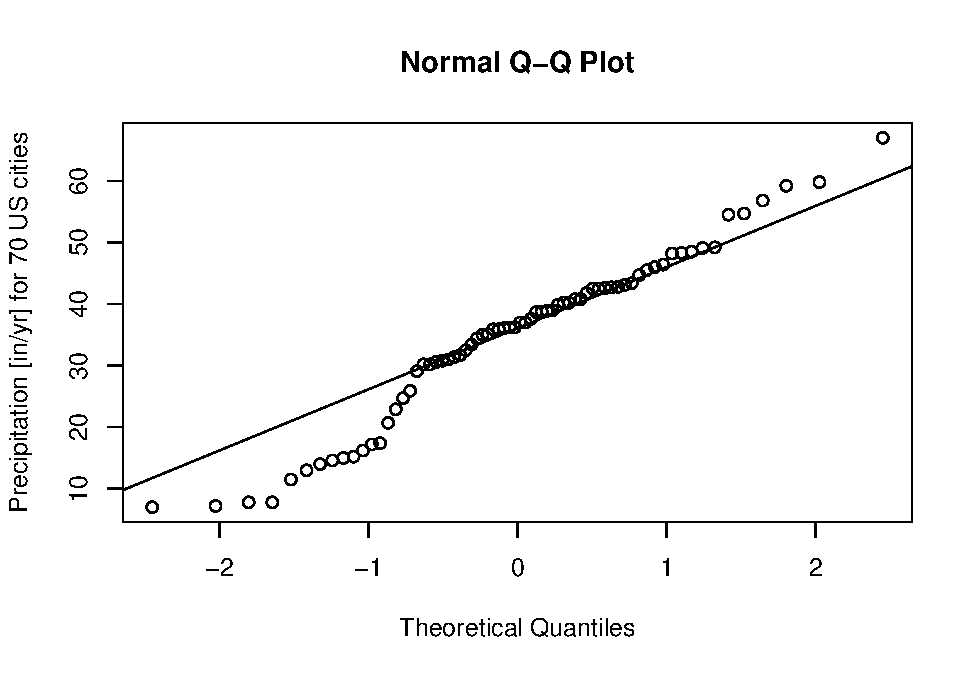
\includegraphics{02-prerequisites_files/figure-latex/unnamed-chunk-4-1.pdf}

\textbf{MGF}

\[
m_X(t) = \frac{pe^t}{1-qe^t}
\]

for \(t < -ln(q)\)

\textbf{Mean}

\[
\mu = \frac{1}{p}
\]

\textbf{Variance}

\[
\sigma^2 = Var(X) = \frac{q}{p^2}
\]

\hypertarget{hypergeometric}{%
\paragraph{Hypergeometric}\label{hypergeometric}}

\begin{itemize}
\tightlist
\item
  The experiment consists of drawing a random sample of size n without replacement and without regard to order from a collection of N objects.
\item
  Of the N objects, r have a trait of interest; N-r do not have the trait
\item
  X is the number of objects in the sample with the trait.
\end{itemize}

\textbf{Density}

\[
f(x)=\frac{{{r}\choose{x}}{{N-r}\choose{n-x}}}{{{N}\choose{n}}}
\]

where \(max[0,n-(N-r)] \le x \le min(n,r)\)

\textbf{PDF}

\begin{Shaded}
\begin{Highlighting}[]
\CommentTok{\# hist of hypergeometric distribution with the number of white balls = 50, and the number of black balls = 20, and number of balls drawn = 30. }
\FunctionTok{hist}\NormalTok{(}\FunctionTok{rhyper}\NormalTok{(}\AttributeTok{nn =} \DecValTok{10000}\NormalTok{ , }\AttributeTok{m=}\DecValTok{50}\NormalTok{, }\AttributeTok{n=}\DecValTok{20}\NormalTok{, }\AttributeTok{k=}\DecValTok{30}\NormalTok{))}
\end{Highlighting}
\end{Shaded}

\includegraphics{02-prerequisites_files/figure-latex/unnamed-chunk-5-1.pdf}

\textbf{Mean}

\[
\mu = E(x)= \frac{nr}{N}
\]

\textbf{Variance}

\[
\sigma^2 = var(X) = n (\frac{r}{N})(\frac{N-r}{N})(\frac{N-n}{N-1})
\]

\textbf{Note} For large N (if \(\frac{n}{N} \le 0.05\)), this distribution can be approximated using a Binomial distribution with \(p = \frac{r}{N}\)

\hypertarget{section}{%
\paragraph{}\label{section}}

\hypertarget{continuous}{%
\subsubsection{Continuous}\label{continuous}}

\hypertarget{uniform}{%
\paragraph{Uniform}\label{uniform}}

\begin{itemize}
\tightlist
\item
  Defined over an interval (a,b) in which the probabilities are ``equally likely'' for subintervals of equal length.
\end{itemize}

\textbf{Density}

\[
f(x)=\frac{1}{b-a}
\]

for a \textless{} x \textless{} b

\textbf{CDF}

\[
\begin{cases}
0 & \text{if x <a } \\
\frac{x-a}{b-a} & \text{if $a \le x \le b$ }\\
1 & \text{if x >b}\\
\end{cases}
\]

\textbf{PDF}

\begin{Shaded}
\begin{Highlighting}[]
\FunctionTok{hist}\NormalTok{(}\FunctionTok{runif}\NormalTok{(}\DecValTok{100000}\NormalTok{, }\AttributeTok{min =} \DecValTok{0}\NormalTok{, }\AttributeTok{max =} \DecValTok{1}\NormalTok{))}
\end{Highlighting}
\end{Shaded}

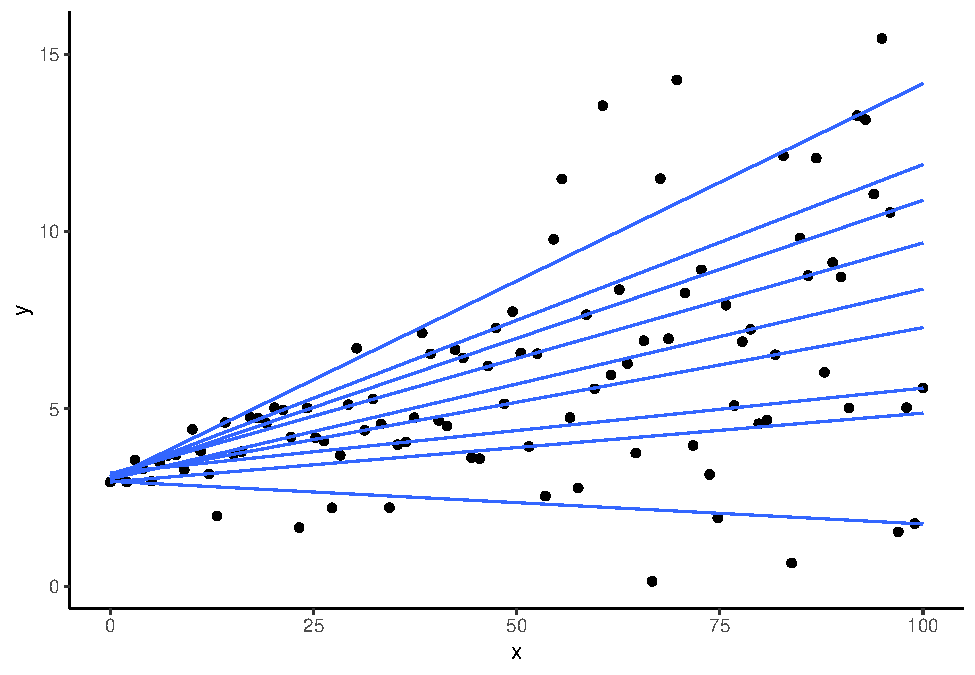
\includegraphics{02-prerequisites_files/figure-latex/unnamed-chunk-6-1.pdf}

\textbf{MGF}

\[
\begin{cases}
\frac{e^{tb} - e^{ta}}{t(b-a)}&\text{ if $t \neq 0$}\\
1&\text{if $ t \neq 0$}\\
\end{cases}
\]

\textbf{Mean}

\[
\mu = E(X) = \frac{a +b}{2}
\]

\textbf{Variance}

\[
\sigma^2 = Var(X) = \frac{(b-a)^2}{12}
\]

\hypertarget{gamma}{%
\paragraph{Gamma}\label{gamma}}

\begin{itemize}
\tightlist
\item
  is used to define the exponential and chi-squared distributions
\item
  The gamma function is defined as:
\end{itemize}

\[
\Gamma(\alpha) = \int_0^{\infty} z^{\alpha-1}e^{-z}dz
\]

where \(\alpha > 0\)

\begin{itemize}
\item
  Properties of The Gamma function:\\

  \begin{itemize}
  \tightlist
  \item
    \(\Gamma(1) = 1\) + For \(\alpha >1\), \(\Gamma(\alpha)=(\alpha-1)\Gamma(\alpha-1)\) + If n is an integer and \(n>1\), then \(\Gamma(n) = (n-1)!\)
  \end{itemize}
\end{itemize}

\textbf{Density}

\[
f(x) = \frac{1}{\Gamma(\alpha)\beta^{\alpha}}x^{\alpha-1}e^{-x/\beta}
\]

\textbf{CDF}

\[
F(x,n,\beta) = 1 -\sum_{k=0}^{n-1} \frac{(\frac{x}{\beta})^k e^{-x/\beta}}{k!}
\]

for x\textgreater0, and \(\alpha = n\) (a positive integer)

\textbf{PDF}

\begin{Shaded}
\begin{Highlighting}[]
\FunctionTok{hist}\NormalTok{(}\FunctionTok{rgamma}\NormalTok{(}\AttributeTok{n =} \DecValTok{10000}\NormalTok{, }\AttributeTok{shape =} \DecValTok{5}\NormalTok{, }\AttributeTok{rate =} \DecValTok{1}\NormalTok{))}
\end{Highlighting}
\end{Shaded}

\includegraphics{02-prerequisites_files/figure-latex/unnamed-chunk-7-1.pdf}

\textbf{MGF}

\[
m_X(t) = (1-\beta t)^{-\alpha}
\]

where \(t < \frac{1}{\beta}\)

\textbf{Mean}

\[
\mu = E(X) = \alpha \beta
\]

\textbf{Variance}

\[
\sigma^2 = Var(X) = \alpha \beta^2
\]

\hypertarget{normal}{%
\paragraph{Normal}\label{normal}}

\(N(\mu,\sigma^2)\)

\begin{itemize}
\tightlist
\item
  is symmetric, bell-shaped curve with parameters \(\mu\) and \(\sigma^2\)
\item
  also known as Gaussian.
\end{itemize}

\textbf{Density}

\[
f(x) = \frac{1}{\sigma \sqrt{2\pi }}e^{-\frac{1}{2}(\frac{x-\mu}{\sigma})^2}
\]

for \(-\infty < x, \mu< \infty, \sigma > 0\)

\textbf{CDF}

Use table

\textbf{PDF}

\begin{Shaded}
\begin{Highlighting}[]
\FunctionTok{hist}\NormalTok{(}\FunctionTok{rnorm}\NormalTok{(}\DecValTok{1000000}\NormalTok{, }\AttributeTok{mean =} \DecValTok{0}\NormalTok{, }\AttributeTok{sd =} \DecValTok{1}\NormalTok{))}
\end{Highlighting}
\end{Shaded}

\includegraphics{02-prerequisites_files/figure-latex/unnamed-chunk-8-1.pdf}

\textbf{MGF}

\[
m_X(t) = e^{\mu t + \frac{\sigma^2 t^2}{2}}
\]

\textbf{Mean}

\[
\mu = E(X)
\]

\textbf{Variance}

\[
\sigma^2 = Var(X)
\]

\textbf{Standard Normal Random Variable}

\begin{itemize}
\tightlist
\item
  The normal random variable Z with mean \(\mu = 0\) and standard deviation \(\sigma =1\) is called standard normal
\item
  Any normal random variable X with mean \(\mu\) and standard deviation \(\sigma\) can be converted to the standard normal random variable \(Z = \frac{X-\mu}{\sigma}\)
\end{itemize}

\textbf{Normal Approximation to the Binomial Distribution}

Let X be binomial with parameters n and p.~For large n (so that \((A)p \le .5\) and \(np > 5\) or (B) \(p>.5\) and \(nq>5\)), X is approximately normally distributed with mean \(\mu = np\) and standard deviation \(\sigma = \sqrt{npq}\)

When using the normal approximation, add or subtract 0.5 as needed for the continuity correction

\begin{longtable}[]{@{}cc@{}}
\toprule
Discrete & Approximate Normal (corrected)\tabularnewline
\midrule
\endhead
P(X = c) & P(c -0.5 \textless{} Y \textless{} c + 0.5)\tabularnewline
P(X \textless{} c) & P(Y \textless{} c - 0.5)\tabularnewline
P(X \le c) & P(Y \textless{} c + 0.5)\tabularnewline
P(X \textgreater{} c) & P(Y \textgreater{} c + 0.5)\tabularnewline
P(X \ge c) & P(Y \textgreater{} c - 0.5)\tabularnewline
\bottomrule
\end{longtable}

\textbf{Normal Probability Rule}

If X is normally distributed with parameters \(\mu\) and \(\sigma\), then

\begin{itemize}
\tightlist
\item
  \(P(-\sigma < X - \mu < \sigma) \approx .68\) * \(P(-2\sigma < X - \mu < 2\sigma) \approx .95\) * \(P(-3\sigma < X - \mu < 3\sigma) \approx .997\)
\end{itemize}

\hypertarget{logistic}{%
\paragraph{Logistic}\label{logistic}}

\(Logistic(\mu,s)\)

\textbf{PDF}

\begin{Shaded}
\begin{Highlighting}[]
\FunctionTok{hist}\NormalTok{(}\FunctionTok{rlogis}\NormalTok{(}\AttributeTok{n =} \DecValTok{100000}\NormalTok{, }\AttributeTok{location =} \DecValTok{0}\NormalTok{, }\AttributeTok{scale =} \DecValTok{1}\NormalTok{))}
\end{Highlighting}
\end{Shaded}

\includegraphics{02-prerequisites_files/figure-latex/unnamed-chunk-9-1.pdf}

\hypertarget{lognomral}{%
\paragraph{Lognomral}\label{lognomral}}

\(lognormal(\mu,\sigma^2)\)

\textbf{PDF}

\begin{Shaded}
\begin{Highlighting}[]
\FunctionTok{hist}\NormalTok{(}\FunctionTok{rlnorm}\NormalTok{(}\AttributeTok{n =} \DecValTok{10000}\NormalTok{, }\AttributeTok{meanlog =} \DecValTok{0}\NormalTok{, }\AttributeTok{sdlog =} \DecValTok{1}\NormalTok{))}
\end{Highlighting}
\end{Shaded}

\includegraphics{02-prerequisites_files/figure-latex/unnamed-chunk-10-1.pdf}

\hypertarget{exponential}{%
\paragraph{Exponential}\label{exponential}}

\(Exp(\lambda)\)

\begin{itemize}
\tightlist
\item
  A special case of the gamma distribution with \(\alpha = 1\)
\item
  Lack of memory
\item
  \(\lambda\) = rate Within a Poisson process with parameter \(\lambda\), if W is the waiting tine until the occurrence of the first event, then W has an exponential distribution with \(\beta = 1/\alpha\)
\end{itemize}

\textbf{Density}

\[
f(x) = \frac{1}{\beta} e^{-x/\beta}
\]

for \(x,\beta > 0\)

\textbf{CDF}

\begin{equation}
F(x) = 
\begin{cases}
0 & \text{ if $x \le 0$}\\
1 - e^{-x/\beta} & \text{if $x > 0$}\\
\end{cases}
\end{equation}

\textbf{PDF}

\begin{Shaded}
\begin{Highlighting}[]
\FunctionTok{hist}\NormalTok{(}\FunctionTok{rexp}\NormalTok{(}\AttributeTok{n =} \DecValTok{100000}\NormalTok{, }\AttributeTok{rate =} \DecValTok{1}\NormalTok{))}
\end{Highlighting}
\end{Shaded}

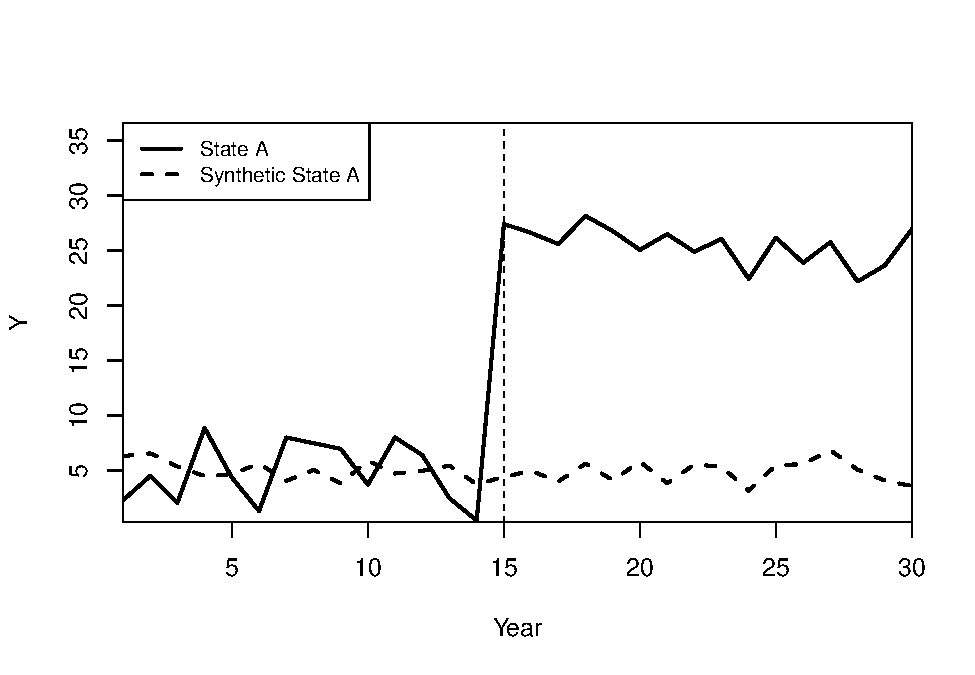
\includegraphics{02-prerequisites_files/figure-latex/unnamed-chunk-11-1.pdf}

\textbf{MGF}

\[
m_X(t) = (1-\beta t)^{-1}
\]

for \(t < 1/\beta\)

\textbf{Mean}

\[
\mu = E(X) = \beta
\]

\textbf{Variance}

\[
\sigma^2 = Var(X) =\beta^2
\]

\hypertarget{chi-squared}{%
\paragraph{Chi-squared}\label{chi-squared}}

\(\chi^2=\chi^2(k)\)

\begin{itemize}
\tightlist
\item
  A special case of the gamma distribution with \(\beta =2\), and \(\alpha = \gamma /2\) for a positive integer \(\gamma\)
\item
  The random variable X is denoted \(\chi_{\gamma}^2\) and is said to have a chi-squared distribution with \(\gamma\) degrees of freedom.
\end{itemize}

\textbf{Density} Use density for Gamma Distribution with \(\beta = 2\) and \(\alpha = \gamma/2\)

\textbf{CDF} Use table

\textbf{PDF}

\begin{Shaded}
\begin{Highlighting}[]
\FunctionTok{hist}\NormalTok{(}\FunctionTok{rchisq}\NormalTok{(}\AttributeTok{n =} \DecValTok{10000}\NormalTok{, }\AttributeTok{df=}\DecValTok{2}\NormalTok{, }\AttributeTok{ncp =} \DecValTok{0}\NormalTok{))}
\end{Highlighting}
\end{Shaded}

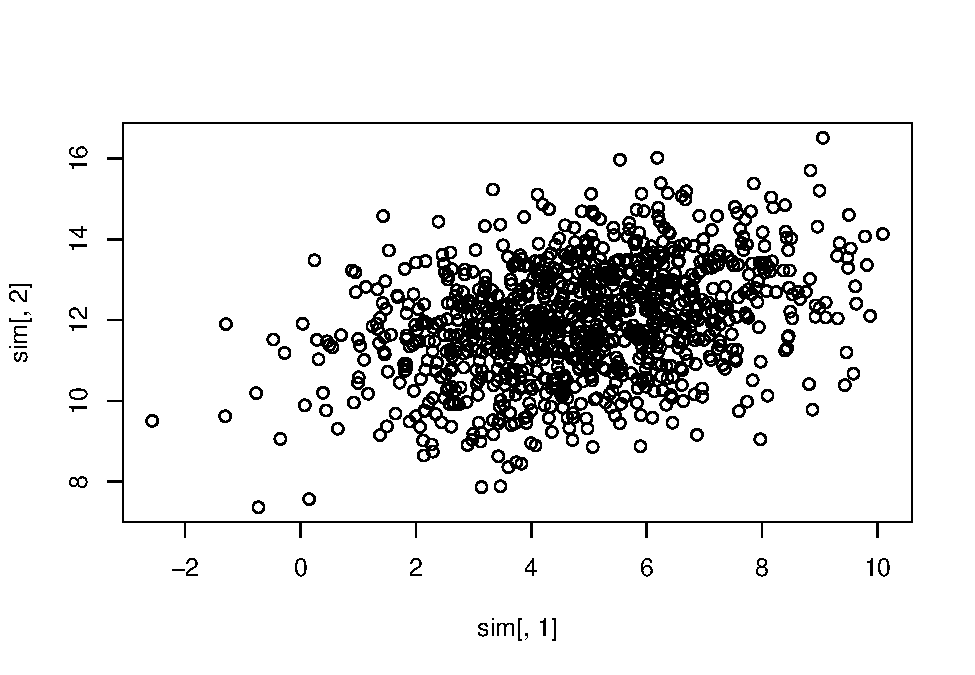
\includegraphics{02-prerequisites_files/figure-latex/unnamed-chunk-12-1.pdf}

\textbf{MGF}

\[
m_X(t) = (1-2t)^{-\gamma/2}
\]

\textbf{Mean}

\[
\mu = E(X) = \gamma
\]

\textbf{Variance}

\[
\sigma^2 = Var(X) = 2\gamma
\]

\hypertarget{student-t}{%
\paragraph{Student T}\label{student-t}}

\(T(v)\)

\begin{itemize}
\tightlist
\item
  \(T=\frac{Z}{\sqrt{\chi_{\gamma}^2/\gamma}}\), where Z is standard normal follows a student-t distribution with \(\gamma\) dof
\item
  The distribution is symmetric, bell-shaped , with a mean of \(\mu=0\)
\end{itemize}

\begin{Shaded}
\begin{Highlighting}[]
\FunctionTok{hist}\NormalTok{(}\FunctionTok{rt}\NormalTok{(}\AttributeTok{n =} \DecValTok{100000}\NormalTok{, }\AttributeTok{df=}\DecValTok{2}\NormalTok{, }\AttributeTok{ncp =}\DecValTok{1}\NormalTok{))}
\end{Highlighting}
\end{Shaded}

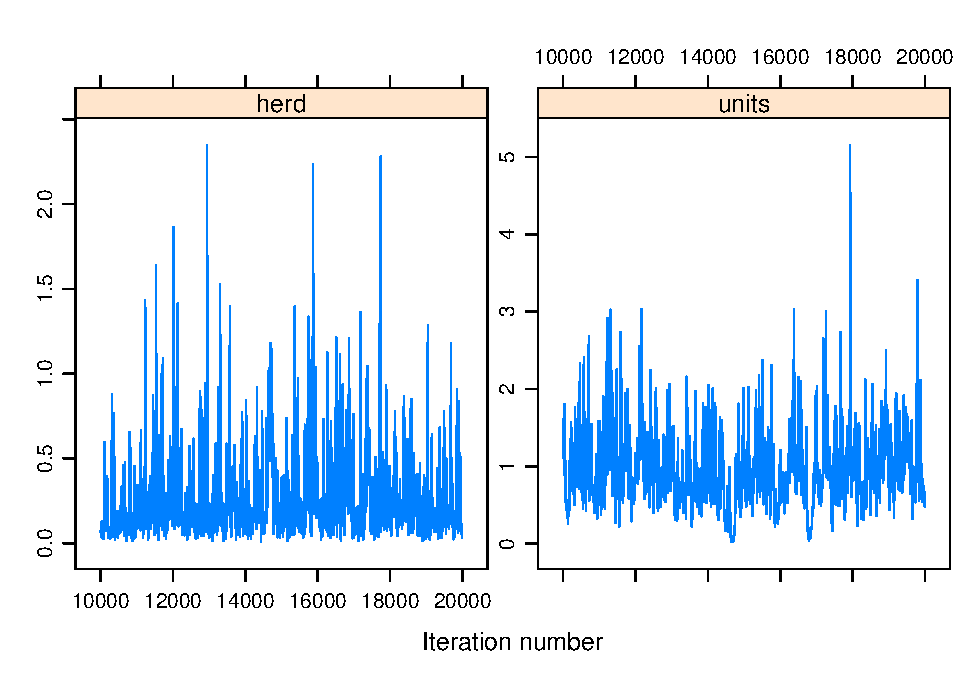
\includegraphics{02-prerequisites_files/figure-latex/unnamed-chunk-13-1.pdf}

\hypertarget{f-distribution}{%
\paragraph{F-Distribution}\label{f-distribution}}

\(F(d_1,d_2)\)

\begin{itemize}
\tightlist
\item
  F distribution is strictly positive
\item
  \(F=\frac{\chi_{\gamma_1}^2/\gamma_1}{\chi_{\gamma_2^2}/\gamma_2}\) follows an F distribution with dof \(\gamma_1\) and \(\gamma_2\), where \(\chi_{\gamma_1}^2\) and \(\chi_{\gamma_2}^2\) are independent chi-squared random variables.
\item
  The distribution is asymmetric and never negative.
\end{itemize}

\textbf{PDF}

\begin{Shaded}
\begin{Highlighting}[]
\FunctionTok{hist}\NormalTok{(}\FunctionTok{rf}\NormalTok{(}\AttributeTok{n =} \DecValTok{100000}\NormalTok{, }\AttributeTok{df1=}\DecValTok{2}\NormalTok{, }\AttributeTok{df2=}\DecValTok{3}\NormalTok{, }\AttributeTok{ncp=}\DecValTok{1}\NormalTok{))}
\end{Highlighting}
\end{Shaded}

\includegraphics{02-prerequisites_files/figure-latex/unnamed-chunk-14-1.pdf}

\hypertarget{cauchy}{%
\paragraph{Cauchy}\label{cauchy}}

\protect\hyperlink{central-limit-theorem}{Central Limit Theorem} and \protect\hyperlink{weak-law}{Weak Law} do not apply to Cauchy because it does not have finite mean and finite variance

\textbf{PDF}

\begin{Shaded}
\begin{Highlighting}[]
\FunctionTok{hist}\NormalTok{(}\FunctionTok{rcauchy}\NormalTok{(}\AttributeTok{n =} \DecValTok{100000}\NormalTok{, }\AttributeTok{location =} \DecValTok{0}\NormalTok{, }\AttributeTok{scale =} \DecValTok{1}\NormalTok{))}
\end{Highlighting}
\end{Shaded}

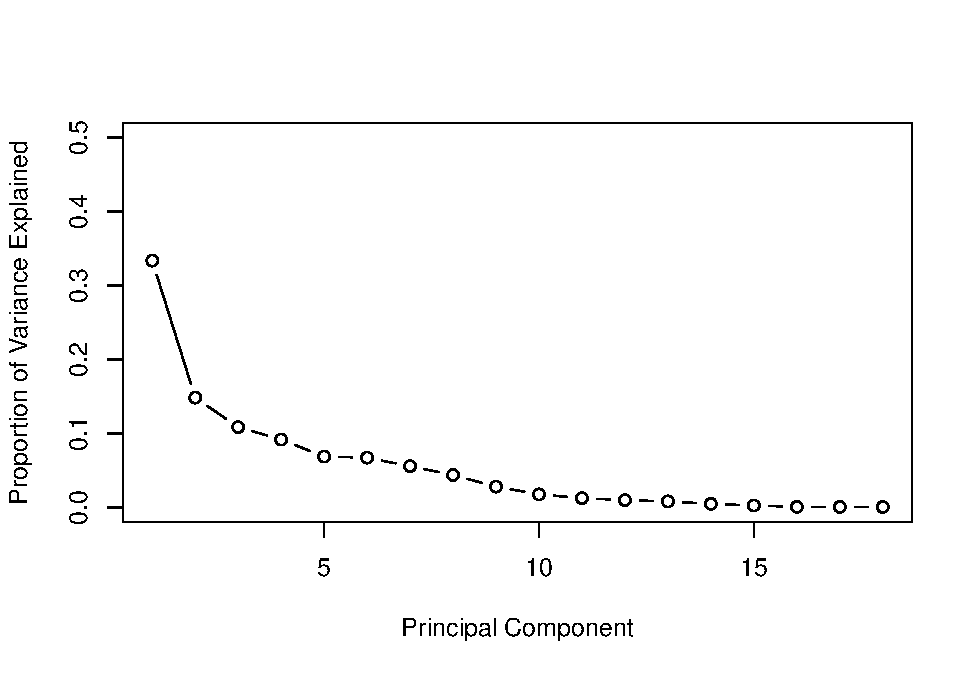
\includegraphics{02-prerequisites_files/figure-latex/unnamed-chunk-15-1.pdf}

\hypertarget{multivariate-normal-distribution}{%
\paragraph{Multivariate Normal Distribution}\label{multivariate-normal-distribution}}

Let y be a p-dimensional multivariate normal (MVN) rv with mean \(\mu\) and variance \(\Sigma\). Then, the density of y is

\[
f(\mathbf{y}) = \frac{1}{(2\pi)^{p/2}|\mathbf{\Sigma}|^{1/2}}exp(-\frac{1}{2}\mathbf{(y-\mu)'\Sigma^{-1}(y-\mu)})
\]

We have \(\mathbf{y} \sim N_p(\mathbf{\mu,\Sigma})\)

Properties:

\begin{itemize}
\tightlist
\item
  Let \(\mathbf{A}_{r \times p}\) be a fixed matrix. then \(\mathbf{Ay} \sim N_r(\mathbf{A \mu, A \Sigma A')}\). Note that \(r \le p\) and all rows of A must be linearly independent to guarantee that \(\mathbf{A\Sigma A'}\) is non-singular.\\
\item
  Let \(\mathbf{G}\) be a matrix such that \(\mathbf{\Sigma^{-1}= GG'}\). then, \(\mathbf{G'y} \sim N_p (\mathbf{G'\mu,I})\) and \(\mathbf{G'(y-\mu)} \sim N_p (\mathbf{0,I})\).\\
\item
  Any fixed linear combination of \(y_1,...,y_p\) say \(\mathbf{c'y}\), follows \(\mathbf{c'y} \sim N_1(\mathbf{c'\mu,c'\Sigma c})\)
\end{itemize}

\textbf{Large Sample Properties}

Suppose that \(y_1,...,y_n\) are a random sample from some population with mean \(\mu\) and variance-variance matrix \(\Sigma\)

\[
\mathbf{Y} \sim MVN(\mathbf{\mu,\Sigma})
\]

Then

\begin{itemize}
\tightlist
\item
  \(\bar{\mathbf{y}} = \frac{1}{n}\sum_{i=1}^n \mathbf{y}_i\) is a consistent estimator for \(\mathbf{\mu}\)\\
\item
  \(\mathbf{S} = \frac{1}{n-1}\sum_{i=1}^n \mathbf{(y_i - \bar{y})(y_i - \bar{y})'}\) is a consistent estimator for \(\mathbf{\Sigma}\)\\
\item
  Multivariate Central Limit Theorem: Similar to the univariate case, \(\sqrt{n}(\mathbf{\bar{y}- \mu}) \sim N_p(\mathbf{0, \Sigma})\) when n is large relative to p (e.g., \(n \ge 25p\)), which is equivalent to \(\bar{y} \sim N_p(\mathbf{\mu,\Sigma/n})\)\\
\item
  Wald's Theorem: \(n(\mathbf{\bar{y}- \mu)'S^{-1}(\bar{y}- \mu)} \sim \chi^2_{(p)}\) when n is large relative to p.
\end{itemize}

\hypertarget{section-1}{%
\paragraph{}\label{section-1}}

\hypertarget{general-math}{%
\section{General Math}\label{general-math}}

\textbf{Chebyshev's Inequality} Let X be a random variable with mean \(\mu\) and standard deviation \(\sigma\). Then for any positive number k:

\[
P(|X-\mu| < k\sigma) \ge 1 - \frac{1}{k^2}
\]

Chebyshev's Inequality does not require that X be normally distributed

\textbf{Maclaurin series expansion for}

\[
e^z = 1 + z + \frac{z^2}{2!} + \frac{z^3}{3!} + ...
\]

\textbf{Geometric series:}

\[
s_n=\sum_{k=1}^{n}ar^{n-1}=\frac{a(1-r^n)}{1-r}
\]

if \textbar r\textbar{} \textless{} 1

\[
s=\sum_{k=1}^{\infty}ar^{n-1}=\frac{a}{1-r}
\]

\hypertarget{law-of-large-numbers}{%
\subsection{Law of large numbers}\label{law-of-large-numbers}}

Let \(X_1,X_2,...\) be an infinite sequence of independent and identically distributed (i.i.d) Then, the sample average is

\[
\bar{X}_n =\frac{1}{n} (X_1 + ... + X_n)
\]

converges to the expected value (\(\bar{X}_n \rightarrow \mu\)) as \(n \rightarrow \infty\)

\[
Var(X_i) = Var(\frac{1}{n}(X_1 + ... + X_n)) = \frac{1}{n^2}Var(X_1 + ... + X_n)= \frac{n\sigma^2}{n^2}=\frac{\sigma^2}{n}
\]

The difference between \protect\hyperlink{weak-law}{Weak Law} and \protect\hyperlink{strong-law}{Strong Law} regards the mode of convergence

\hypertarget{weak-law}{%
\subsubsection{Weak Law}\label{weak-law}}

The sample average converges in probability towards the expected value

\[
\bar{X}_n \rightarrow^{p} \mu
\]

when \(n \rightarrow \infty\)

\[
\lim_{n\to \infty}P(|\bar{X}_n - \mu| > \epsilon) = 0
\]

The sample mean from a iid random sample (\(\{ x_i \}_{i=1}^n\)) from any population with a finite mean and finite variance \(\sigma^2\) is ca consistent estimation for the population mean \(\mu\)

\[
plim(\bar{x})=plim(n^{-1}\sum_{i=1}^{n}x_i) =\mu
\]

\hypertarget{strong-law}{%
\subsubsection{Strong Law}\label{strong-law}}

The sample average converges almost surely to the expected value

\[
\bar{X}_n \rightarrow^{a.s} \mu 
\]

when \(n \rightarrow \infty\)

Equivalently,

\[
P(\lim_{n\to \infty}\bar{X}_n =\mu) =1
\]

\hypertarget{law-of-iterated-expectation}{%
\subsection{Law of Iterated Expectation}\label{law-of-iterated-expectation}}

Let X, Y be random variables. Then,

\[
E(X) = E(E(X|Y))
\]

means that the expected value of X can be calculated from the probability distribution of X\textbar Y and Y

\hypertarget{convergence}{%
\subsection{Convergence}\label{convergence}}

\hypertarget{convergence-in-probability}{%
\subsubsection{Convergence in Probability}\label{convergence-in-probability}}

\begin{itemize}
\tightlist
\item
  \(n \rightarrow \infty\), an estimator (random variable) that is close to the true value.
\item
  The random variable \(\theta_n\) converges in probability to a constant c if
\end{itemize}

\[
\lim_{n\to \infty}P(|\theta_n - c| \ge \epsilon) = 0
\]

for any positive \(\epsilon\)

Notation

\[
plim(\theta_n)=c 
\]

Equivalently,

\[
\theta_n \rightarrow^p c
\]

\textbf{Properties of Convergence in Probability}

\begin{itemize}
\item
  Slutsky's Theorem: for a continuous function g(.), if \(plim(\theta_n)= \theta\) then \(plim(g(\theta_n)) = g(\theta)\)
\item
  if \(\gamma_n \rightarrow^p \gamma\) then\\

  \begin{itemize}
  \tightlist
  \item
    \(plim(\theta_n + \gamma_n)=\theta + \gamma\) + \(plim(\theta_n \gamma_n) = \theta \gamma\) + \(plim(\theta_n/\gamma_n) = \theta/\gamma\) if \(\gamma \neq 0\)
  \end{itemize}
\item
  Also hold for random vectors/ matrices
\end{itemize}

\hypertarget{convergence-in-distribution}{%
\subsubsection{Convergence in Distribution}\label{convergence-in-distribution}}

\begin{itemize}
\tightlist
\item
  As \(n \rightarrow \infty\), the distribution of a random variable may converge towards another (``fixed'') distribution.
\item
  The random variable \(X_n\) with CDF \(F_n(x)\) converges in distribution to a random variable X with CDF \(F(X)\) if
\end{itemize}

\[
\lim_{n\to \infty}|F_n(x) - F(x)| = 0
\]

at all points of continuity of \(F(X)\)

Notation F(x) is the limiting distribution of \(X_n\) or \(X_n \rightarrow^d X\)

\begin{itemize}
\tightlist
\item
  E(X) is the limiting mean (asymptotic mean)
\item
  Var(X) is the limiting variance (asymptotic variance)
\end{itemize}

\textbf{Note}

\[
E(X) \neq \lim_{n\to \infty}E(X_n) \\
Avar(X_n) \neq \lim_{n\to \infty}Var(X_n)
\]

\textbf{Properties of Convergence in Distribution}

\begin{itemize}
\item
  Continuous Mapping Theorem: for a continuous function g(.), if \(X_n \to^{d} g(X)\) then \(g(X_n) \to^{d} g(X)\)
\item
  if \(Y_n\to^{d} c\), then

  \begin{itemize}
  \item
    \(X_n + Y_n \to^{d} X + c\)
  \item
    \(Y_nX_n \to^{d} cX\)
  \item
    \(X_nY_n \to^{d} X/c\) if \(c \neq 0\)
  \end{itemize}
\item
  also hold for random vectors/matrices
\end{itemize}

\hypertarget{summary}{%
\subsubsection{Summary}\label{summary}}

Properties of Convergence

\begin{longtable}[]{@{}ll@{}}
\toprule
\begin{minipage}[b]{(\columnwidth - 1\tabcolsep) * \real{0.52}}\raggedright
Probability\strut
\end{minipage} & \begin{minipage}[b]{(\columnwidth - 1\tabcolsep) * \real{0.48}}\raggedright
Distribution\strut
\end{minipage}\tabularnewline
\midrule
\endhead
\begin{minipage}[t]{(\columnwidth - 1\tabcolsep) * \real{0.52}}\raggedright
Slutsky's Theorem: for a continuous function g(.), if \(plim(\theta_n)= \theta\) then \(plim(g(\theta_n)) = g(\theta)\)\strut
\end{minipage} & \begin{minipage}[t]{(\columnwidth - 1\tabcolsep) * \real{0.48}}\raggedright
Continuous Mapping Theorem: for a continuous function g(.), if \(X_n \to^{d} g(X)\) then \(g(X_n) \to^{d} g(X)\)\strut
\end{minipage}\tabularnewline
\begin{minipage}[t]{(\columnwidth - 1\tabcolsep) * \real{0.52}}\raggedright
if \(\gamma_n \rightarrow^p \gamma\) then\strut
\end{minipage} & \begin{minipage}[t]{(\columnwidth - 1\tabcolsep) * \real{0.48}}\raggedright
if \(Y_n\to^{d} c\), then\strut
\end{minipage}\tabularnewline
\begin{minipage}[t]{(\columnwidth - 1\tabcolsep) * \real{0.52}}\raggedright
\(plim(\theta_n + \gamma_n)=\theta + \gamma\)\strut
\end{minipage} & \begin{minipage}[t]{(\columnwidth - 1\tabcolsep) * \real{0.48}}\raggedright
\(X_n + Y_n \to^{d} X + c\)\strut
\end{minipage}\tabularnewline
\begin{minipage}[t]{(\columnwidth - 1\tabcolsep) * \real{0.52}}\raggedright
\(plim(\theta_n \gamma_n) = \theta \gamma\)\strut
\end{minipage} & \begin{minipage}[t]{(\columnwidth - 1\tabcolsep) * \real{0.48}}\raggedright
\(Y_nX_n \to^{d} cX\)\strut
\end{minipage}\tabularnewline
\begin{minipage}[t]{(\columnwidth - 1\tabcolsep) * \real{0.52}}\raggedright
\(plim(\theta_n/\gamma_n) = \theta/\gamma\) if \(\gamma \neq 0\)\strut
\end{minipage} & \begin{minipage}[t]{(\columnwidth - 1\tabcolsep) * \real{0.48}}\raggedright
\(X_nY_n \to^{d} X/c\) if \(c \neq 0\)\strut
\end{minipage}\tabularnewline
\bottomrule
\end{longtable}

\protect\hyperlink{convergence-in-probability}{Convergence in Probability} is stronger than \protect\hyperlink{convergence-in-distribution}{Convergence in Distribution}. However, \protect\hyperlink{convergence-in-distribution}{Convergence in Distribution} does not guarantee \protect\hyperlink{convergence-in-probability}{Convergence in Probability}

\hypertarget{sufficient-statistics}{%
\subsection{Sufficient Statistics}\label{sufficient-statistics}}

\textbf{Likelihood}

\begin{itemize}
\tightlist
\item
  describes the extent to which the sample provides support for any particular parameter value.
\item
  Higher support corresponds to a higher value for the likelihood
\item
  The exact value of any likelihood is \textbf{meaningless},
\item
  The relative value, (i.e., comparing two values of \(\theta\)), is \textbf{informative}.
\end{itemize}

\[
L(\theta_0; y) = P(Y = y | \theta = \theta_0) = f_Y(y;\theta_0)
\]

\textbf{Likelihood Ratio}

\[
\frac{L(\theta_0;y)}{L(\theta_1;y)}
\]

\textbf{Likelihood Function}

For a given sample, you can create likelihoods for all possible values of \(\theta\), which is called \emph{likelihood function}

\[
L(\theta) = L(\theta; y) = f_Y(y;\theta)
\]

In a sample of size n, the likelihood function takes the form of a product

\[
L(\theta) = \prod_{i=1}^{n}f_i (y_i;\theta)
\]

Equivalently, the log likelihood function

\[
l(\theta) = \sum_{i=1}^{n} logf_i(y_i;\theta)
\]

\textbf{Sufficient statistics}

\begin{itemize}
\tightlist
\item
  A statistic, T(y), is any quantity that can be calculated purely from a sample (independent of \(\theta\))
\item
  A statistic is \textbf{sufficient} if it conveys all the available information about the parameter.
\end{itemize}

\[
L(\theta; y) = c(y)L^*(\theta;T(y))
\]

\textbf{Nuisance parameters} If we are interested in a parameter (e.g., mean). Other parameters requiring estimation (e.g., standard deviation) are \textbf{nuisance} parameters. We can replace nuisance parameters in likelihood function with their estimates to create a **profile likelihood*.

\hypertarget{parameter-transformations}{%
\subsection{Parameter transformations}\label{parameter-transformations}}

log-odds transformation

\[
Log odds = g(\theta)= ln[\frac{\theta}{1-\theta}]
\]

log transformation

\hypertarget{methods}{%
\section{Methods}\label{methods}}

Trade-off between parametric and non-parametric

\hypertarget{data-importexport}{%
\section{Data Import/Export}\label{data-importexport}}

\href{https://cran.r-project.org/doc/manuals/r-release/R-data.html}{Extended Manual by R}

\begin{longtable}[]{@{}lllll@{}}
\caption{Table by \href{https://cran.r-project.org/web/packages/rio/vignettes/rio.html}{Rio Vignette}}\tabularnewline
\toprule
Format & Typical Extension & Import Package & Export Package & Installed by Default\tabularnewline
\midrule
\endfirsthead
\toprule
Format & Typical Extension & Import Package & Export Package & Installed by Default\tabularnewline
\midrule
\endhead
Comma-separated data & .csv & \href{https://cran.r-project.org/package=data.table}{\textbf{data.table}} & \href{https://cran.r-project.org/package=data.table}{\textbf{data.table}} & Yes\tabularnewline
Pipe-separated data & .psv & \href{https://cran.r-project.org/package=data.table}{\textbf{data.table}} & \href{https://cran.r-project.org/package=data.table}{\textbf{data.table}} & Yes\tabularnewline
Tab-separated data & .tsv & \href{https://cran.r-project.org/package=data.table}{\textbf{data.table}} & \href{https://cran.r-project.org/package=data.table}{\textbf{data.table}} & Yes\tabularnewline
CSVY (CSV + YAML metadata header) & .csvy & \href{https://cran.r-project.org/package=data.table}{\textbf{data.table}} & \href{https://cran.r-project.org/package=data.table}{\textbf{data.table}} & Yes\tabularnewline
SAS & .sas7bdat & \href{https://cran.r-project.org/package=haven}{\textbf{haven}} & \href{https://cran.r-project.org/package=haven}{\textbf{haven}} & Yes\tabularnewline
SPSS & .sav & \href{https://cran.r-project.org/package=haven}{\textbf{haven}} & \href{https://cran.r-project.org/package=haven}{\textbf{haven}} & Yes\tabularnewline
SPSS (compressed) & .zsav & \href{https://cran.r-project.org/package=haven}{\textbf{haven}} & \href{https://cran.r-project.org/package=haven}{\textbf{haven}} & Yes\tabularnewline
Stata & .dta & \href{https://cran.r-project.org/package=haven}{\textbf{haven}} & \href{https://cran.r-project.org/package=haven}{\textbf{haven}} & Yes\tabularnewline
SAS XPORT & .xpt & \href{https://cran.r-project.org/package=haven}{\textbf{haven}} & \href{https://cran.r-project.org/package=haven}{\textbf{haven}} & Yes\tabularnewline
SPSS Portable & .por & \href{https://cran.r-project.org/package=haven}{\textbf{haven}} & & Yes\tabularnewline
Excel & .xls & \href{https://cran.r-project.org/package=readxl}{\textbf{readxl}} & & Yes\tabularnewline
Excel & .xlsx & \href{https://cran.r-project.org/package=readxl}{\textbf{readxl}} & \href{https://cran.r-project.org/package=openxlsx}{\textbf{openxlsx}} & Yes\tabularnewline
R syntax & .R & \textbf{base} & \textbf{base} & Yes\tabularnewline
Saved R objects & .RData, .rda & \textbf{base} & \textbf{base} & Yes\tabularnewline
Serialized R objects & .rds & \textbf{base} & \textbf{base} & Yes\tabularnewline
Epiinfo & .rec & \href{https://cran.r-project.org/package=foreign}{\textbf{foreign}} & & Yes\tabularnewline
Minitab & .mtp & \href{https://cran.r-project.org/package=foreign}{\textbf{foreign}} & & Yes\tabularnewline
Systat & .syd & \href{https://cran.r-project.org/package=foreign}{\textbf{foreign}} & & Yes\tabularnewline
``XBASE'' database files & .dbf & \href{https://cran.r-project.org/package=foreign}{\textbf{foreign}} & \href{https://cran.r-project.org/package=foreign}{\textbf{foreign}} & Yes\tabularnewline
Weka Attribute-Relation File Format & .arff & \href{https://cran.r-project.org/package=foreign}{\textbf{foreign}} & \href{https://cran.r-project.org/package=foreign}{\textbf{foreign}} & Yes\tabularnewline
Data Interchange Format & .dif & \textbf{utils} & & Yes\tabularnewline
Fortran data & no recognized extension & \textbf{utils} & & Yes\tabularnewline
Fixed-width format data & .fwf & \textbf{utils} & \textbf{utils} & Yes\tabularnewline
gzip comma-separated data & .csv.gz & \textbf{utils} & \textbf{utils} & Yes\tabularnewline
Apache Arrow (Parquet) & .parquet & \href{https://cran.r-project.org/package=arrow}{\textbf{arrow}} & \href{https://cran.r-project.org/package=arrow}{\textbf{arrow}} & No\tabularnewline
EViews & .wf1 & \href{https://cran.r-project.org/package=hexView}{\textbf{hexView}} & & No\tabularnewline
Feather R/Python interchange format & .feather & \href{https://cran.r-project.org/package=feather}{\textbf{feather}} & \href{https://cran.r-project.org/package=feather}{\textbf{feather}} & No\tabularnewline
Fast Storage & .fst & \href{https://cran.r-project.org/package=fst}{\textbf{fst}} & \href{https://cran.r-project.org/package=fst}{\textbf{fst}} & No\tabularnewline
JSON & .json & \href{https://cran.r-project.org/package=jsonlite}{\textbf{jsonlite}} & \href{https://cran.r-project.org/package=jsonlite}{\textbf{jsonlite}} & No\tabularnewline
Matlab & .mat & \href{https://cran.r-project.org/package=rmatio}{\textbf{rmatio}} & \href{https://cran.r-project.org/package=rmatio}{\textbf{rmatio}} & No\tabularnewline
OpenDocument Spreadsheet & .ods & \href{https://cran.r-project.org/package=readODS}{\textbf{readODS}} & \href{https://cran.r-project.org/package=readODS}{\textbf{readODS}} & No\tabularnewline
HTML Tables & .html & \href{https://cran.r-project.org/package=xml2}{\textbf{xml2}} & \href{https://cran.r-project.org/package=xml2}{\textbf{xml2}} & No\tabularnewline
Shallow XML documents & .xml & \href{https://cran.r-project.org/package=xml2}{\textbf{xml2}} & \href{https://cran.r-project.org/package=xml2}{\textbf{xml2}} & No\tabularnewline
YAML & .yml & \href{https://cran.r-project.org/package=yaml}{\textbf{yaml}} & \href{https://cran.r-project.org/package=yaml}{\textbf{yaml}} & No\tabularnewline
Clipboard & default is tsv & \href{https://cran.r-project.org/package=clipr}{\textbf{clipr}} & \href{https://cran.r-project.org/package=clipr}{\textbf{clipr}} & No\tabularnewline
\href{https://www.google.com/sheets/about/}{Google Sheets} & as Comma-separated data & & &\tabularnewline
\bottomrule
\end{longtable}

R limitations:

\begin{itemize}
\item
  By default, R use 1 core in CPU
\item
  R puts data into memory (limit around 2-4 GB), while SAS uses data from files on demand
\item
  Categorization

  \begin{itemize}
  \item
    Medium-size file: within RAM limit, around 1-2 GB
  \item
    Large file: 2-10 GB, there might be some workaround solution
  \item
    Very large file \textgreater{} 10 GB, you have to use distributed or parallel computing
  \end{itemize}
\end{itemize}

Solutions:

\begin{itemize}
\item
  buy more RAM
\item
  HPC packages

  \begin{itemize}
  \item
    Explicit Parallelism
  \item
    Implicit Parallelism
  \item
    Large Memory
  \item
    Map/Reduce
  \end{itemize}
\end{itemize}

\begin{itemize}
\item
  specify number of rows and columns, typically including command \texttt{nrow\ =}
\item
  Use packages that store data differently

  \begin{itemize}
  \item
    \texttt{bigmemory}, \texttt{biganalytics}, \texttt{bigtabulate} , \texttt{synchronicity}, \texttt{bigalgebra}, \texttt{bigvideo} use C++ to store matrices, but also support one class type
  \item
    For multiple class types, use \texttt{ff} package
  \end{itemize}
\item
  Very Large datasets use

  \begin{itemize}
  \tightlist
  \item
    \texttt{RHaddop} package
  \item
    \texttt{HadoopStreaming}
  \item
    \texttt{Rhipe}
  \end{itemize}
\end{itemize}

\hypertarget{medium-size}{%
\subsection{Medium size}\label{medium-size}}

\begin{Shaded}
\begin{Highlighting}[]
\FunctionTok{library}\NormalTok{(}\StringTok{"rio"}\NormalTok{)}
\end{Highlighting}
\end{Shaded}

\begin{verbatim}
## Warning: package 'rio' was built under R version 4.0.5
\end{verbatim}

To import multiple files in a directory

\begin{Shaded}
\begin{Highlighting}[]
\FunctionTok{str}\NormalTok{(}\FunctionTok{import\_list}\NormalTok{(}\FunctionTok{dir}\NormalTok{()), }\AttributeTok{which =} \DecValTok{1}\NormalTok{)}
\end{Highlighting}
\end{Shaded}

To export a single data file

\begin{Shaded}
\begin{Highlighting}[]
\FunctionTok{export}\NormalTok{(data, }\StringTok{"data.csv"}\NormalTok{)}
\FunctionTok{export}\NormalTok{(data,}\StringTok{"data.dta"}\NormalTok{)}
\FunctionTok{export}\NormalTok{(data,}\StringTok{"data.txt"}\NormalTok{)}
\FunctionTok{export}\NormalTok{(data,}\StringTok{"data\_cyl.rds"}\NormalTok{)}
\FunctionTok{export}\NormalTok{(data,}\StringTok{"data.rdata"}\NormalTok{)}
\FunctionTok{export}\NormalTok{(data,}\StringTok{"data.R"}\NormalTok{)}
\FunctionTok{export}\NormalTok{(data,}\StringTok{"data.csv.zip"}\NormalTok{)}
\FunctionTok{export}\NormalTok{(data,}\StringTok{"list.json"}\NormalTok{)}
\end{Highlighting}
\end{Shaded}

To export multiple data files

\begin{Shaded}
\begin{Highlighting}[]
\FunctionTok{export}\NormalTok{(}\FunctionTok{list}\NormalTok{(}\AttributeTok{mtcars =}\NormalTok{ mtcars, }\AttributeTok{iris =}\NormalTok{ iris), }\StringTok{"data\_file\_type"}\NormalTok{) }\CommentTok{\# where data\_file\_type should substituted with the extension listed above}
\end{Highlighting}
\end{Shaded}

To convert between data file types

\begin{Shaded}
\begin{Highlighting}[]
\CommentTok{\# convert Stata to SPSS}
\FunctionTok{convert}\NormalTok{(}\StringTok{"data.dta"}\NormalTok{, }\StringTok{"data.sav"}\NormalTok{)}
\end{Highlighting}
\end{Shaded}

\hypertarget{large-size}{%
\subsection{Large size}\label{large-size}}

Use R on a cluster

\begin{itemize}
\tightlist
\item
  Amazon Web Service (AWS): \$1/hr
\end{itemize}

Import files as chunks

\begin{Shaded}
\begin{Highlighting}[]
\NormalTok{file\_in    }\OtherTok{\textless{}{-}} \FunctionTok{file}\NormalTok{(}\StringTok{"in.csv"}\NormalTok{,}\StringTok{"r"}\NormalTok{)}
\NormalTok{chunk\_size }\OtherTok{\textless{}{-}} \DecValTok{100000} \CommentTok{\# choose the best size for you}
\NormalTok{x          }\OtherTok{\textless{}{-}} \FunctionTok{readLines}\NormalTok{(file\_in, }\AttributeTok{n=}\NormalTok{chunk\_size)}
\end{Highlighting}
\end{Shaded}

\texttt{data.table} method

\begin{Shaded}
\begin{Highlighting}[]
\FunctionTok{require}\NormalTok{(data.table)}
\NormalTok{mydata }\OtherTok{=} \FunctionTok{fread}\NormalTok{(}\StringTok{"in.csv"}\NormalTok{, }\AttributeTok{header =}\NormalTok{ T)}
\end{Highlighting}
\end{Shaded}

\texttt{ff} package: this method does not allow you to pass connections

\begin{Shaded}
\begin{Highlighting}[]
\FunctionTok{library}\NormalTok{(}\StringTok{"ff"}\NormalTok{)}
\NormalTok{x }\OtherTok{\textless{}{-}} \FunctionTok{read.csv.ffdf}\NormalTok{(}
    \AttributeTok{file =} \StringTok{"file.csv"}\NormalTok{,}
    \AttributeTok{nrow =} \DecValTok{10}\NormalTok{,}
    \AttributeTok{header =} \ConstantTok{TRUE}\NormalTok{,}
    \AttributeTok{VERBOSE =} \ConstantTok{TRUE}\NormalTok{,}
    \AttributeTok{first.rows =} \DecValTok{10000}\NormalTok{,}
    \AttributeTok{next.rows =} \DecValTok{50000}\NormalTok{,}
    \AttributeTok{colClasses =} \ConstantTok{NA}
\NormalTok{)}
\end{Highlighting}
\end{Shaded}

\texttt{bigmemory} package

\begin{Shaded}
\begin{Highlighting}[]
\NormalTok{my\_data }\OtherTok{\textless{}{-}} \FunctionTok{read.big.matrix}\NormalTok{(}\StringTok{\textquotesingle{}in.csv\textquotesingle{}}\NormalTok{, }\AttributeTok{header =}\NormalTok{ T)}
\end{Highlighting}
\end{Shaded}

\texttt{sqldf} package

\begin{Shaded}
\begin{Highlighting}[]
\FunctionTok{library}\NormalTok{(sqldf)}
\NormalTok{my\_data }\OtherTok{\textless{}{-}} \FunctionTok{read.csv.sql}\NormalTok{(}\StringTok{\textquotesingle{}in.csv\textquotesingle{}}\NormalTok{)}

\NormalTok{iris2 }\OtherTok{\textless{}{-}} \FunctionTok{read.csv.sql}\NormalTok{(}\StringTok{"iris.csv"}\NormalTok{, }
    \AttributeTok{sql =} \StringTok{"select * from file where Species = \textquotesingle{}setosa\textquotesingle{} "}\NormalTok{)}
\end{Highlighting}
\end{Shaded}

\begin{Shaded}
\begin{Highlighting}[]
\FunctionTok{library}\NormalTok{(RMySQL)}
\end{Highlighting}
\end{Shaded}

\begin{verbatim}
## Warning: package 'RMySQL' was built under R version 4.0.5
\end{verbatim}

\begin{verbatim}
## Loading required package: DBI
\end{verbatim}

\texttt{RQLite} package

\begin{itemize}
\tightlist
\item
  \href{https://sqlite.org/download.html}{Download SQLite}, pick ``A bundle of command-line tools for managing SQLite database files'' for Window 10
\item
  Unzip file, and open \texttt{sqlite3.exe.}
\item
  Type in the prompt

  \begin{itemize}
  \tightlist
  \item
    \texttt{sqlite\textgreater{}\ .cd\ \textquotesingle{}C:\textbackslash{}Users\textbackslash{}data\textquotesingle{}} specify path to your desired directory
  \item
    \texttt{sqlite\textgreater{}\ .open\ database\_name.db} to open a database
  \item
    To import the CSV file into the database

    \begin{itemize}
    \tightlist
    \item
      \texttt{sqlite\textgreater{}\ .mode\ csv} specify to SQLite that the next file is .csv file
    \item
      \texttt{sqlite\textgreater{}\ .import\ file\_name.csv\ datbase\_name} to import the csv file to the database
    \end{itemize}
  \item
    \texttt{sqlite\textgreater{}\ .exit} After you're done, exit the sqlite program
  \end{itemize}
\end{itemize}

\begin{Shaded}
\begin{Highlighting}[]
\FunctionTok{library}\NormalTok{(DBI)}
\FunctionTok{library}\NormalTok{(dplyr)}
\FunctionTok{library}\NormalTok{(}\StringTok{"RSQLite"}\NormalTok{)}
\FunctionTok{setwd}\NormalTok{(}\StringTok{""}\NormalTok{)}
\NormalTok{con }\OtherTok{\textless{}{-}} \FunctionTok{dbConnect}\NormalTok{(RSQLite}\SpecialCharTok{::}\FunctionTok{SQLite}\NormalTok{(), }\StringTok{"data\_base.db"}\NormalTok{)}
\NormalTok{tbl }\OtherTok{\textless{}{-}} \FunctionTok{tbl}\NormalTok{(con, }\StringTok{"data\_table"}\NormalTok{)}
\NormalTok{tbl }\SpecialCharTok{\%\textgreater{}\%} 
    \FunctionTok{filter}\NormalTok{() }\SpecialCharTok{\%\textgreater{}\%}
    \FunctionTok{select}\NormalTok{() }\SpecialCharTok{\%\textgreater{}\%}
    \FunctionTok{collect}\NormalTok{() }\CommentTok{\# to actually pull the data into the workspace}
\FunctionTok{dbDisconnect}\NormalTok{(con)}
\end{Highlighting}
\end{Shaded}

\texttt{arrow} package

\begin{Shaded}
\begin{Highlighting}[]
\FunctionTok{library}\NormalTok{(}\StringTok{"arrow"}\NormalTok{)}
\FunctionTok{read\_csv\_arrow}\NormalTok{()}
\end{Highlighting}
\end{Shaded}

\texttt{vroom} package

\begin{Shaded}
\begin{Highlighting}[]
\FunctionTok{library}\NormalTok{(vroom)}
\FunctionTok{spec}\NormalTok{(}\FunctionTok{vroom}\NormalTok{(file\_path))}
\NormalTok{compressed }\OtherTok{\textless{}{-}} \FunctionTok{vroom\_example}\NormalTok{(}\StringTok{"mtcars.csv.zip"}\NormalTok{)}
\FunctionTok{vroom}\NormalTok{(compressed)}
\end{Highlighting}
\end{Shaded}

\texttt{data.table} package

\begin{Shaded}
\begin{Highlighting}[]
\NormalTok{s }\OtherTok{=} \FunctionTok{fread}\NormalTok{(}\StringTok{"sample.csv"}\NormalTok{)}
\end{Highlighting}
\end{Shaded}

Comparisons regarding storage space

\begin{Shaded}
\begin{Highlighting}[]
\NormalTok{test }\OtherTok{=}\NormalTok{ ff}\SpecialCharTok{::}\FunctionTok{read.csv.ffdf}\NormalTok{(}\AttributeTok{file =} \StringTok{""}\NormalTok{)}
\FunctionTok{object.size}\NormalTok{(test) }\CommentTok{\# worst}

\NormalTok{test1 }\OtherTok{=}\NormalTok{ data.table}\SpecialCharTok{::}\FunctionTok{fread}\NormalTok{(}\AttributeTok{file =} \StringTok{""}\NormalTok{)}
\FunctionTok{object.size}\NormalTok{(test1) }\CommentTok{\# best}

\NormalTok{test2 }\OtherTok{=}\NormalTok{ readr}\SpecialCharTok{::}\FunctionTok{read\_csv}\NormalTok{(}\StringTok{""}\NormalTok{)}\ErrorTok{)}
\FunctionTok{object.size}\NormalTok{(test2) }\CommentTok{\# 2nd}

\NormalTok{test3 }\OtherTok{=} \FunctionTok{vroom}\NormalTok{(}\AttributeTok{file =} \StringTok{""}\NormalTok{)}
\FunctionTok{object.size}\NormalTok{(test3) }\CommentTok{\# equal to read\_csv}
\end{Highlighting}
\end{Shaded}

To work with big data, you can convert it to \texttt{csv.gz} , but since typically, R would require you to load the whole data then export it. With data greater than 10 GB, we have to do it sequentially. Even though \texttt{read.csv} is much slower than \texttt{readr::read\_csv} , we still have to use it because it can pass connection, and it allows you to loop sequentially. On the other, because currently \texttt{readr::read\_csv} does not have the \texttt{skip} function, and even if we can use the skip, we still have to read and skip lines in previous loop.

For example, say you \texttt{read\_csv(,\ n\_max\ =\ 100,\ skip\ =0)} and then \texttt{read\_csv(,\ n\_max\ =\ 200,\ skip\ =\ 100)} you actually have to read again the first 100 rows. However, \texttt{read.csv} without specifying anything, will continue at the 100 mark.

Notice, sometimes you might have error looking like this

``Error in (function (con, what, n = 1L, size = NA\_integer\_, signed = TRUE, : can only read from a binary connection''

then you can change it instead of \texttt{r} in the connection into \texttt{rb} . Even though an author of the package suggested that \texttt{file} should be able to recognize the appropriate form, so far I did not prevail.

\hypertarget{data-manipulation}{%
\section{Data Manipulation}\label{data-manipulation}}

\begin{Shaded}
\begin{Highlighting}[]
\CommentTok{\# load packages}
\FunctionTok{library}\NormalTok{(tidyverse)}
\end{Highlighting}
\end{Shaded}

\begin{verbatim}
## Warning: package 'tidyverse' was built under R version 4.0.5
\end{verbatim}

\begin{verbatim}
## -- Attaching packages --------------------------------------- tidyverse 1.3.1 --
\end{verbatim}

\begin{verbatim}
## v ggplot2 3.3.5     v purrr   0.3.4
## v tibble  3.1.2     v dplyr   1.0.6
## v tidyr   1.1.3     v stringr 1.4.0
## v readr   2.0.1     v forcats 0.5.1
\end{verbatim}

\begin{verbatim}
## Warning: package 'ggplot2' was built under R version 4.0.5
\end{verbatim}

\begin{verbatim}
## Warning: package 'readr' was built under R version 4.0.5
\end{verbatim}

\begin{verbatim}
## Warning: package 'dplyr' was built under R version 4.0.5
\end{verbatim}

\begin{verbatim}
## -- Conflicts ------------------------------------------ tidyverse_conflicts() --
## x dplyr::filter() masks stats::filter()
## x dplyr::lag()    masks stats::lag()
\end{verbatim}

\begin{Shaded}
\begin{Highlighting}[]
\FunctionTok{library}\NormalTok{(lubridate)}
\end{Highlighting}
\end{Shaded}

\begin{verbatim}
## Warning: package 'lubridate' was built under R version 4.0.5
\end{verbatim}

\begin{verbatim}
## 
## Attaching package: 'lubridate'
\end{verbatim}

\begin{verbatim}
## The following objects are masked from 'package:base':
## 
##     date, intersect, setdiff, union
\end{verbatim}

\begin{Shaded}
\begin{Highlighting}[]
\NormalTok{x }\OtherTok{\textless{}{-}} \FunctionTok{c}\NormalTok{(}\DecValTok{1}\NormalTok{, }\DecValTok{4}\NormalTok{, }\DecValTok{23}\NormalTok{, }\DecValTok{4}\NormalTok{, }\DecValTok{45}\NormalTok{)}
\NormalTok{n }\OtherTok{\textless{}{-}} \FunctionTok{c}\NormalTok{(}\DecValTok{1}\NormalTok{, }\DecValTok{3}\NormalTok{, }\DecValTok{5}\NormalTok{)}
\NormalTok{g }\OtherTok{\textless{}{-}} \FunctionTok{c}\NormalTok{(}\StringTok{"M"}\NormalTok{, }\StringTok{"M"}\NormalTok{, }\StringTok{"F"}\NormalTok{)}
\NormalTok{df }\OtherTok{\textless{}{-}} \FunctionTok{data.frame}\NormalTok{(n, g)}
\NormalTok{df}
\end{Highlighting}
\end{Shaded}

\begin{verbatim}
##   n g
## 1 1 M
## 2 3 M
## 3 5 F
\end{verbatim}

\begin{Shaded}
\begin{Highlighting}[]
\FunctionTok{str}\NormalTok{(df)}
\end{Highlighting}
\end{Shaded}

\begin{verbatim}
## 'data.frame':    3 obs. of  2 variables:
##  $ n: num  1 3 5
##  $ g: chr  "M" "M" "F"
\end{verbatim}

\begin{Shaded}
\begin{Highlighting}[]
\CommentTok{\#Similarly}
\NormalTok{df }\OtherTok{\textless{}{-}} \FunctionTok{tibble}\NormalTok{(n, g)}
\NormalTok{df}
\end{Highlighting}
\end{Shaded}

\begin{verbatim}
## # A tibble: 3 x 2
##       n g    
##   <dbl> <chr>
## 1     1 M    
## 2     3 M    
## 3     5 F
\end{verbatim}

\begin{Shaded}
\begin{Highlighting}[]
\FunctionTok{str}\NormalTok{(df)}
\end{Highlighting}
\end{Shaded}

\begin{verbatim}
## tibble [3 x 2] (S3: tbl_df/tbl/data.frame)
##  $ n: num [1:3] 1 3 5
##  $ g: chr [1:3] "M" "M" "F"
\end{verbatim}

\begin{Shaded}
\begin{Highlighting}[]
\CommentTok{\# list form}
\NormalTok{lst }\OtherTok{\textless{}{-}} \FunctionTok{list}\NormalTok{(x, n, g, df)}
\NormalTok{lst}
\end{Highlighting}
\end{Shaded}

\begin{verbatim}
## [[1]]
## [1]  1  4 23  4 45
## 
## [[2]]
## [1] 1 3 5
## 
## [[3]]
## [1] "M" "M" "F"
## 
## [[4]]
## # A tibble: 3 x 2
##       n g    
##   <dbl> <chr>
## 1     1 M    
## 2     3 M    
## 3     5 F
\end{verbatim}

\begin{Shaded}
\begin{Highlighting}[]
\CommentTok{\# Or}
\NormalTok{lst2 }\OtherTok{\textless{}{-}} \FunctionTok{list}\NormalTok{(}\AttributeTok{num =}\NormalTok{ x, }\AttributeTok{size =}\NormalTok{ n, }\AttributeTok{sex =}\NormalTok{ g, }\AttributeTok{data =}\NormalTok{ df)}
\NormalTok{lst2}
\end{Highlighting}
\end{Shaded}

\begin{verbatim}
## $num
## [1]  1  4 23  4 45
## 
## $size
## [1] 1 3 5
## 
## $sex
## [1] "M" "M" "F"
## 
## $data
## # A tibble: 3 x 2
##       n g    
##   <dbl> <chr>
## 1     1 M    
## 2     3 M    
## 3     5 F
\end{verbatim}

\begin{Shaded}
\begin{Highlighting}[]
\CommentTok{\# Or}
\NormalTok{lst3 }\OtherTok{\textless{}{-}} \FunctionTok{list}\NormalTok{(}\AttributeTok{x =} \FunctionTok{c}\NormalTok{(}\DecValTok{1}\NormalTok{, }\DecValTok{3}\NormalTok{, }\DecValTok{5}\NormalTok{, }\DecValTok{7}\NormalTok{),}
             \AttributeTok{y =} \FunctionTok{c}\NormalTok{(}\DecValTok{2}\NormalTok{, }\DecValTok{2}\NormalTok{, }\DecValTok{2}\NormalTok{, }\DecValTok{4}\NormalTok{, }\DecValTok{5}\NormalTok{, }\DecValTok{5}\NormalTok{, }\DecValTok{5}\NormalTok{, }\DecValTok{6}\NormalTok{),}
             \AttributeTok{z =} \FunctionTok{c}\NormalTok{(}\DecValTok{22}\NormalTok{, }\DecValTok{3}\NormalTok{, }\DecValTok{3}\NormalTok{, }\DecValTok{3}\NormalTok{, }\DecValTok{5}\NormalTok{, }\DecValTok{10}\NormalTok{))}
\NormalTok{lst3}
\end{Highlighting}
\end{Shaded}

\begin{verbatim}
## $x
## [1] 1 3 5 7
## 
## $y
## [1] 2 2 2 4 5 5 5 6
## 
## $z
## [1] 22  3  3  3  5 10
\end{verbatim}

\begin{Shaded}
\begin{Highlighting}[]
\CommentTok{\# find the means of x, y, z.}

\CommentTok{\# can do one at a time}
\FunctionTok{mean}\NormalTok{(lst3}\SpecialCharTok{$}\NormalTok{x)}
\end{Highlighting}
\end{Shaded}

\begin{verbatim}
## [1] 4
\end{verbatim}

\begin{Shaded}
\begin{Highlighting}[]
\FunctionTok{mean}\NormalTok{(lst3}\SpecialCharTok{$}\NormalTok{y)}
\end{Highlighting}
\end{Shaded}

\begin{verbatim}
## [1] 3.875
\end{verbatim}

\begin{Shaded}
\begin{Highlighting}[]
\FunctionTok{mean}\NormalTok{(lst3}\SpecialCharTok{$}\NormalTok{z)}
\end{Highlighting}
\end{Shaded}

\begin{verbatim}
## [1] 7.666667
\end{verbatim}

\begin{Shaded}
\begin{Highlighting}[]
\CommentTok{\# list apply}
\FunctionTok{lapply}\NormalTok{(lst3, mean)}
\end{Highlighting}
\end{Shaded}

\begin{verbatim}
## $x
## [1] 4
## 
## $y
## [1] 3.875
## 
## $z
## [1] 7.666667
\end{verbatim}

\begin{Shaded}
\begin{Highlighting}[]
\CommentTok{\# OR}
\FunctionTok{sapply}\NormalTok{(lst3, mean)}
\end{Highlighting}
\end{Shaded}

\begin{verbatim}
##        x        y        z 
## 4.000000 3.875000 7.666667
\end{verbatim}

\begin{Shaded}
\begin{Highlighting}[]
\CommentTok{\# Or, tidyverse function map() }
\FunctionTok{map}\NormalTok{(lst3, mean)}
\end{Highlighting}
\end{Shaded}

\begin{verbatim}
## $x
## [1] 4
## 
## $y
## [1] 3.875
## 
## $z
## [1] 7.666667
\end{verbatim}

\begin{Shaded}
\begin{Highlighting}[]
\CommentTok{\# The tidyverse requires a modified map function called map\_dbl()}
\FunctionTok{map\_dbl}\NormalTok{(lst3, mean)}
\end{Highlighting}
\end{Shaded}

\begin{verbatim}
##        x        y        z 
## 4.000000 3.875000 7.666667
\end{verbatim}

\begin{Shaded}
\begin{Highlighting}[]
\CommentTok{\# Binding }
\NormalTok{dat01 }\OtherTok{\textless{}{-}} \FunctionTok{tibble}\NormalTok{(}\AttributeTok{x =} \DecValTok{1}\SpecialCharTok{:}\DecValTok{5}\NormalTok{, }\AttributeTok{y =} \DecValTok{5}\SpecialCharTok{:}\DecValTok{1}\NormalTok{)}
\NormalTok{dat01}
\end{Highlighting}
\end{Shaded}

\begin{verbatim}
## # A tibble: 5 x 2
##       x     y
##   <int> <int>
## 1     1     5
## 2     2     4
## 3     3     3
## 4     4     2
## 5     5     1
\end{verbatim}

\begin{Shaded}
\begin{Highlighting}[]
\NormalTok{dat02 }\OtherTok{\textless{}{-}} \FunctionTok{tibble}\NormalTok{(}\AttributeTok{x =} \DecValTok{10}\SpecialCharTok{:}\DecValTok{16}\NormalTok{, }\AttributeTok{y =}\NormalTok{ x}\SpecialCharTok{/}\DecValTok{2}\NormalTok{)}
\NormalTok{dat02}
\end{Highlighting}
\end{Shaded}

\begin{verbatim}
## # A tibble: 7 x 2
##       x     y
##   <int> <dbl>
## 1    10   5  
## 2    11   5.5
## 3    12   6  
## 4    13   6.5
## 5    14   7  
## 6    15   7.5
## 7    16   8
\end{verbatim}

\begin{Shaded}
\begin{Highlighting}[]
\NormalTok{dat03 }\OtherTok{\textless{}{-}} \FunctionTok{tibble}\NormalTok{(}\AttributeTok{z =} \FunctionTok{runif}\NormalTok{(}\DecValTok{5}\NormalTok{)) }\CommentTok{\# 5 random numbers from interval (0,1)}
\NormalTok{dat03}
\end{Highlighting}
\end{Shaded}

\begin{verbatim}
## # A tibble: 5 x 1
##       z
##   <dbl>
## 1 0.532
## 2 0.580
## 3 0.868
## 4 0.884
## 5 0.657
\end{verbatim}

\begin{Shaded}
\begin{Highlighting}[]
\CommentTok{\# row binding}
\FunctionTok{bind\_rows}\NormalTok{(dat01, dat02, dat01)}
\end{Highlighting}
\end{Shaded}

\begin{verbatim}
## # A tibble: 17 x 2
##        x     y
##    <int> <dbl>
##  1     1   5  
##  2     2   4  
##  3     3   3  
##  4     4   2  
##  5     5   1  
##  6    10   5  
##  7    11   5.5
##  8    12   6  
##  9    13   6.5
## 10    14   7  
## 11    15   7.5
## 12    16   8  
## 13     1   5  
## 14     2   4  
## 15     3   3  
## 16     4   2  
## 17     5   1
\end{verbatim}

\begin{Shaded}
\begin{Highlighting}[]
\CommentTok{\# use ".id" argument to create a new column that contains an identifier for the original data.}
\FunctionTok{bind\_rows}\NormalTok{(dat01, dat02, }\AttributeTok{.id =} \StringTok{"id"}\NormalTok{)}
\end{Highlighting}
\end{Shaded}

\begin{verbatim}
## # A tibble: 12 x 3
##    id        x     y
##    <chr> <int> <dbl>
##  1 1         1   5  
##  2 1         2   4  
##  3 1         3   3  
##  4 1         4   2  
##  5 1         5   1  
##  6 2        10   5  
##  7 2        11   5.5
##  8 2        12   6  
##  9 2        13   6.5
## 10 2        14   7  
## 11 2        15   7.5
## 12 2        16   8
\end{verbatim}

\begin{Shaded}
\begin{Highlighting}[]
\CommentTok{\# with name}
\FunctionTok{bind\_rows}\NormalTok{(}\StringTok{"dat01"} \OtherTok{=}\NormalTok{ dat01, }\StringTok{"dat02"} \OtherTok{=}\NormalTok{ dat02, }\AttributeTok{.id =} \StringTok{"id"}\NormalTok{)}
\end{Highlighting}
\end{Shaded}

\begin{verbatim}
## # A tibble: 12 x 3
##    id        x     y
##    <chr> <int> <dbl>
##  1 dat01     1   5  
##  2 dat01     2   4  
##  3 dat01     3   3  
##  4 dat01     4   2  
##  5 dat01     5   1  
##  6 dat02    10   5  
##  7 dat02    11   5.5
##  8 dat02    12   6  
##  9 dat02    13   6.5
## 10 dat02    14   7  
## 11 dat02    15   7.5
## 12 dat02    16   8
\end{verbatim}

\begin{Shaded}
\begin{Highlighting}[]
\CommentTok{\# bind\_rows() also works on lists of data frames}
\NormalTok{list01 }\OtherTok{\textless{}{-}} \FunctionTok{list}\NormalTok{(}\StringTok{"dat01"} \OtherTok{=}\NormalTok{ dat01, }\StringTok{"dat02"} \OtherTok{=}\NormalTok{ dat02)}
\NormalTok{list01}
\end{Highlighting}
\end{Shaded}

\begin{verbatim}
## $dat01
## # A tibble: 5 x 2
##       x     y
##   <int> <int>
## 1     1     5
## 2     2     4
## 3     3     3
## 4     4     2
## 5     5     1
## 
## $dat02
## # A tibble: 7 x 2
##       x     y
##   <int> <dbl>
## 1    10   5  
## 2    11   5.5
## 3    12   6  
## 4    13   6.5
## 5    14   7  
## 6    15   7.5
## 7    16   8
\end{verbatim}

\begin{Shaded}
\begin{Highlighting}[]
\FunctionTok{bind\_rows}\NormalTok{(list01)}
\end{Highlighting}
\end{Shaded}

\begin{verbatim}
## # A tibble: 12 x 2
##        x     y
##    <int> <dbl>
##  1     1   5  
##  2     2   4  
##  3     3   3  
##  4     4   2  
##  5     5   1  
##  6    10   5  
##  7    11   5.5
##  8    12   6  
##  9    13   6.5
## 10    14   7  
## 11    15   7.5
## 12    16   8
\end{verbatim}

\begin{Shaded}
\begin{Highlighting}[]
\FunctionTok{bind\_rows}\NormalTok{(list01, }\AttributeTok{.id =} \StringTok{"source"}\NormalTok{)}
\end{Highlighting}
\end{Shaded}

\begin{verbatim}
## # A tibble: 12 x 3
##    source     x     y
##    <chr>  <int> <dbl>
##  1 dat01      1   5  
##  2 dat01      2   4  
##  3 dat01      3   3  
##  4 dat01      4   2  
##  5 dat01      5   1  
##  6 dat02     10   5  
##  7 dat02     11   5.5
##  8 dat02     12   6  
##  9 dat02     13   6.5
## 10 dat02     14   7  
## 11 dat02     15   7.5
## 12 dat02     16   8
\end{verbatim}

\begin{Shaded}
\begin{Highlighting}[]
\CommentTok{\# The extended example below demonstrates how this can be very handy.}

\CommentTok{\# column binding}
\FunctionTok{bind\_cols}\NormalTok{(dat01, dat03)}
\end{Highlighting}
\end{Shaded}

\begin{verbatim}
## # A tibble: 5 x 3
##       x     y     z
##   <int> <int> <dbl>
## 1     1     5 0.532
## 2     2     4 0.580
## 3     3     3 0.868
## 4     4     2 0.884
## 5     5     1 0.657
\end{verbatim}

\begin{Shaded}
\begin{Highlighting}[]
\CommentTok{\# Regular expressions {-}{-}{-}{-}{-}{-}{-}{-}{-}{-}{-}{-}{-}{-}{-}{-}{-}{-}{-}{-}{-}{-}{-}{-}{-}{-}{-}{-}{-}{-}{-}{-}{-}{-}{-}{-}{-}{-}{-}{-}{-}{-}{-}{-}{-}{-}{-}{-}{-}{-}{-}{-}{-}}
\NormalTok{names }\OtherTok{\textless{}{-}} \FunctionTok{c}\NormalTok{(}\StringTok{"Ford, MS"}\NormalTok{, }\StringTok{"Jones, PhD"}\NormalTok{, }\StringTok{"Martin, Phd"}\NormalTok{, }\StringTok{"Huck, MA, MLS"}\NormalTok{)}

\CommentTok{\# pattern: first comma and everything after it}
\FunctionTok{str\_remove}\NormalTok{(names, }\AttributeTok{pattern =} \StringTok{", [[:print:]]+"}\NormalTok{)}
\end{Highlighting}
\end{Shaded}

\begin{verbatim}
## [1] "Ford"   "Jones"  "Martin" "Huck"
\end{verbatim}

\begin{Shaded}
\begin{Highlighting}[]
\CommentTok{\# [[:print:]]+ = one or more printable characters}


\CommentTok{\# Reshaping {-}{-}{-}{-}{-}{-}{-}{-}{-}{-}{-}{-}{-}{-}{-}{-}{-}{-}{-}{-}{-}{-}{-}{-}{-}{-}{-}{-}{-}{-}{-}{-}{-}{-}{-}{-}{-}{-}{-}{-}{-}{-}{-}{-}{-}{-}{-}{-}{-}{-}{-}{-}{-}{-}{-}{-}{-}{-}{-}{-}{-}{-}{-}}

\CommentTok{\# Example of a wide data frame. Notice each person has multiple test scores}
\CommentTok{\# that span columns.}
\NormalTok{wide }\OtherTok{\textless{}{-}} \FunctionTok{data.frame}\NormalTok{(}\AttributeTok{name=}\FunctionTok{c}\NormalTok{(}\StringTok{"Clay"}\NormalTok{,}\StringTok{"Garrett"}\NormalTok{,}\StringTok{"Addison"}\NormalTok{), }
                   \AttributeTok{test1=}\FunctionTok{c}\NormalTok{(}\DecValTok{78}\NormalTok{, }\DecValTok{93}\NormalTok{, }\DecValTok{90}\NormalTok{), }
                   \AttributeTok{test2=}\FunctionTok{c}\NormalTok{(}\DecValTok{87}\NormalTok{, }\DecValTok{91}\NormalTok{, }\DecValTok{97}\NormalTok{),}
                   \AttributeTok{test3=}\FunctionTok{c}\NormalTok{(}\DecValTok{88}\NormalTok{, }\DecValTok{99}\NormalTok{, }\DecValTok{91}\NormalTok{))}
\NormalTok{wide}
\end{Highlighting}
\end{Shaded}

\begin{verbatim}
##      name test1 test2 test3
## 1    Clay    78    87    88
## 2 Garrett    93    91    99
## 3 Addison    90    97    91
\end{verbatim}

\begin{Shaded}
\begin{Highlighting}[]
\CommentTok{\# Example of a long data frame. This is the same data as above, but in long}
\CommentTok{\# format. We have one row per person per test.}
\NormalTok{long }\OtherTok{\textless{}{-}} \FunctionTok{data.frame}\NormalTok{(}\AttributeTok{name=}\FunctionTok{rep}\NormalTok{(}\FunctionTok{c}\NormalTok{(}\StringTok{"Clay"}\NormalTok{,}\StringTok{"Garrett"}\NormalTok{,}\StringTok{"Addison"}\NormalTok{),}\AttributeTok{each=}\DecValTok{3}\NormalTok{),}
                   \AttributeTok{test=}\FunctionTok{rep}\NormalTok{(}\DecValTok{1}\SpecialCharTok{:}\DecValTok{3}\NormalTok{, }\DecValTok{3}\NormalTok{),}
                   \AttributeTok{score=}\FunctionTok{c}\NormalTok{(}\DecValTok{78}\NormalTok{, }\DecValTok{87}\NormalTok{, }\DecValTok{88}\NormalTok{, }\DecValTok{93}\NormalTok{, }\DecValTok{91}\NormalTok{, }\DecValTok{99}\NormalTok{, }\DecValTok{90}\NormalTok{, }\DecValTok{97}\NormalTok{, }\DecValTok{91}\NormalTok{))}
\NormalTok{long}
\end{Highlighting}
\end{Shaded}

\begin{verbatim}
##      name test score
## 1    Clay    1    78
## 2    Clay    2    87
## 3    Clay    3    88
## 4 Garrett    1    93
## 5 Garrett    2    91
## 6 Garrett    3    99
## 7 Addison    1    90
## 8 Addison    2    97
## 9 Addison    3    91
\end{verbatim}

\begin{Shaded}
\begin{Highlighting}[]
\CommentTok{\# mean score per student}
\FunctionTok{aggregate}\NormalTok{(score }\SpecialCharTok{\textasciitilde{}}\NormalTok{ name, }\AttributeTok{data =}\NormalTok{ long, mean)}
\end{Highlighting}
\end{Shaded}

\begin{verbatim}
##      name    score
## 1 Addison 92.66667
## 2    Clay 84.33333
## 3 Garrett 94.33333
\end{verbatim}

\begin{Shaded}
\begin{Highlighting}[]
\FunctionTok{aggregate}\NormalTok{(score }\SpecialCharTok{\textasciitilde{}}\NormalTok{ test, }\AttributeTok{data =}\NormalTok{ long, mean)}
\end{Highlighting}
\end{Shaded}

\begin{verbatim}
##   test    score
## 1    1 87.00000
## 2    2 91.66667
## 3    3 92.66667
\end{verbatim}

\begin{Shaded}
\begin{Highlighting}[]
\CommentTok{\# line plot of scores over test, grouped by name}
\FunctionTok{ggplot}\NormalTok{(long, }\FunctionTok{aes}\NormalTok{(}\AttributeTok{x =} \FunctionTok{factor}\NormalTok{(test), }\AttributeTok{y =}\NormalTok{ score, }\AttributeTok{color =}\NormalTok{ name, }\AttributeTok{group =}\NormalTok{ name)) }\SpecialCharTok{+}
  \FunctionTok{geom\_point}\NormalTok{() }\SpecialCharTok{+}
  \FunctionTok{geom\_line}\NormalTok{() }\SpecialCharTok{+}
  \FunctionTok{xlab}\NormalTok{(}\StringTok{"Test"}\NormalTok{)}
\end{Highlighting}
\end{Shaded}

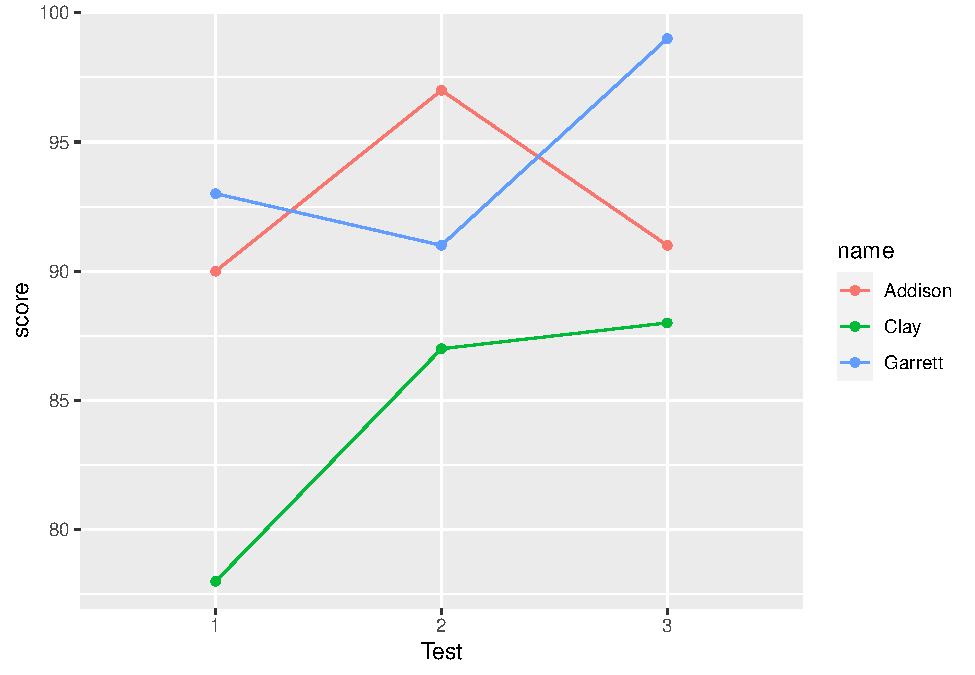
\includegraphics{02-prerequisites_files/figure-latex/unnamed-chunk-32-1.pdf}

\begin{Shaded}
\begin{Highlighting}[]
\DocumentationTok{\#\#\#\# reshape wide to long}
\FunctionTok{pivot\_longer}\NormalTok{(wide, test1}\SpecialCharTok{:}\NormalTok{test3, }\AttributeTok{names\_to =} \StringTok{"test"}\NormalTok{, }\AttributeTok{values\_to =} \StringTok{"score"}\NormalTok{)}
\end{Highlighting}
\end{Shaded}

\begin{verbatim}
## # A tibble: 9 x 3
##   name    test  score
##   <chr>   <chr> <dbl>
## 1 Clay    test1    78
## 2 Clay    test2    87
## 3 Clay    test3    88
## 4 Garrett test1    93
## 5 Garrett test2    91
## 6 Garrett test3    99
## 7 Addison test1    90
## 8 Addison test2    97
## 9 Addison test3    91
\end{verbatim}

\begin{Shaded}
\begin{Highlighting}[]
\CommentTok{\# Or}
\FunctionTok{pivot\_longer}\NormalTok{(wide, }\SpecialCharTok{{-}}\NormalTok{name, }\AttributeTok{names\_to =} \StringTok{"test"}\NormalTok{, }\AttributeTok{values\_to =} \StringTok{"score"}\NormalTok{)}
\end{Highlighting}
\end{Shaded}

\begin{verbatim}
## # A tibble: 9 x 3
##   name    test  score
##   <chr>   <chr> <dbl>
## 1 Clay    test1    78
## 2 Clay    test2    87
## 3 Clay    test3    88
## 4 Garrett test1    93
## 5 Garrett test2    91
## 6 Garrett test3    99
## 7 Addison test1    90
## 8 Addison test2    97
## 9 Addison test3    91
\end{verbatim}

\begin{Shaded}
\begin{Highlighting}[]
\CommentTok{\# drop "test" from the test column with names\_prefix argument}
\FunctionTok{pivot\_longer}\NormalTok{(wide, }\SpecialCharTok{{-}}\NormalTok{name, }\AttributeTok{names\_to =} \StringTok{"test"}\NormalTok{, }\AttributeTok{values\_to =} \StringTok{"score"}\NormalTok{, }
             \AttributeTok{names\_prefix =} \StringTok{"test"}\NormalTok{)}
\end{Highlighting}
\end{Shaded}

\begin{verbatim}
## # A tibble: 9 x 3
##   name    test  score
##   <chr>   <chr> <dbl>
## 1 Clay    1        78
## 2 Clay    2        87
## 3 Clay    3        88
## 4 Garrett 1        93
## 5 Garrett 2        91
## 6 Garrett 3        99
## 7 Addison 1        90
## 8 Addison 2        97
## 9 Addison 3        91
\end{verbatim}

\begin{Shaded}
\begin{Highlighting}[]
\DocumentationTok{\#\#\#\# reshape long to wide }
\FunctionTok{pivot\_wider}\NormalTok{(long, name, }\AttributeTok{names\_from =}\NormalTok{ test, }\AttributeTok{values\_from =}\NormalTok{ score)}
\end{Highlighting}
\end{Shaded}

\begin{verbatim}
## # A tibble: 3 x 4
##   name      `1`   `2`   `3`
##   <chr>   <dbl> <dbl> <dbl>
## 1 Clay       78    87    88
## 2 Garrett    93    91    99
## 3 Addison    90    97    91
\end{verbatim}

\begin{Shaded}
\begin{Highlighting}[]
\CommentTok{\# using the names\_prefix argument lets us prepend text to the column names.}
\FunctionTok{pivot\_wider}\NormalTok{(long, name, }\AttributeTok{names\_from =}\NormalTok{ test, }\AttributeTok{values\_from =}\NormalTok{ score,}
            \AttributeTok{names\_prefix =} \StringTok{"test"}\NormalTok{)}
\end{Highlighting}
\end{Shaded}

\begin{verbatim}
## # A tibble: 3 x 4
##   name    test1 test2 test3
##   <chr>   <dbl> <dbl> <dbl>
## 1 Clay       78    87    88
## 2 Garrett    93    91    99
## 3 Addison    90    97    91
\end{verbatim}

The verbs of data manipulation

\begin{itemize}
\tightlist
\item
  select: selecting (or not selecting) columns based on their names (eg: select columns Q1 through Q25)
\item
  slice: selecting (or not selecting) rows based on their position (eg: select rows 1:10)
\item
  mutate: add or derive new columns (or variables) based on existing columns (eg: create a new column that expresses measurement in cm based on existing measure in inches)
\item
  rename: rename variables or change column names (eg: change ``GraduationRate100'' to ``grad100'')
\item
  filter: selecting rows based on a condition (eg: all rows where gender = Male)
\item
  arrange: ordering rows based on variable(s) numeric or alphabetical order (eg: sort in descending order of Income)
\item
  sample: take random samples of data (eg: sample 80\% of data to create a ``training'' set)
\item
  summarize: condense or aggregate multiple values into single summary values (eg: calculate median income by age group)
\item
  group\_by: convert a tbl into a grouped tbl so that operations are performed ``by group''; allows us to summarize data or apply verbs to data by groups (eg, by gender or treatment)
\item
  the pipe: \%\textgreater\%
\item
  Use Ctrl + Shift + M (Win) or Cmd + Shift + M (Mac) to enter in RStudio
\item
  The pipe takes the output of a function and ``pipes'' into the first argument of the next function.
\end{itemize}

\hypertarget{part-basic}{%
\part{BASIC}\label{part-basic}}

\hypertarget{descriptive-stat}{%
\chapter{Descriptive Statistics}\label{descriptive-stat}}

When you have an area of interest that you want to research, a problem that you want to solve, a relationship that you want to investigate, theoretical and empirical processes will help you.

Estimand is defined as ``a quantity of scientific interest that can be calculated in the population and does not change its value depending on the data collection design used to measure it (i.e., it does not vary with sample size and survey design, or the number of nonrespondents, or follow-up efforts).'' \citep{Rubin_1996}

Estimands include:

\begin{itemize}
\tightlist
\item
  population means
\item
  Population variances
\item
  correlations
\item
  factor loading
\item
  regression coefficients
\end{itemize}

\hypertarget{numerical-measures}{%
\section{Numerical Measures}\label{numerical-measures}}

There are differences between a population and a sample

\begin{longtable}[]{@{}llll@{}}
\toprule
\begin{minipage}[b]{(\columnwidth - 3\tabcolsep) * \real{0.06}}\raggedright
Measures of\strut
\end{minipage} & \begin{minipage}[b]{(\columnwidth - 3\tabcolsep) * \real{0.25}}\raggedright
Category\strut
\end{minipage} & \begin{minipage}[b]{(\columnwidth - 3\tabcolsep) * \real{0.29}}\raggedright
Population\strut
\end{minipage} & \begin{minipage}[b]{(\columnwidth - 3\tabcolsep) * \real{0.40}}\raggedright
Sample\strut
\end{minipage}\tabularnewline
\midrule
\endhead
\begin{minipage}[t]{(\columnwidth - 3\tabcolsep) * \real{0.06}}\raggedright
-\strut
\end{minipage} & \begin{minipage}[t]{(\columnwidth - 3\tabcolsep) * \real{0.25}}\raggedright
What is it?\strut
\end{minipage} & \begin{minipage}[t]{(\columnwidth - 3\tabcolsep) * \real{0.29}}\raggedright
Reality\strut
\end{minipage} & \begin{minipage}[t]{(\columnwidth - 3\tabcolsep) * \real{0.40}}\raggedright
A small fraction of reality (inference)\strut
\end{minipage}\tabularnewline
\begin{minipage}[t]{(\columnwidth - 3\tabcolsep) * \real{0.06}}\raggedright
-\strut
\end{minipage} & \begin{minipage}[t]{(\columnwidth - 3\tabcolsep) * \real{0.25}}\raggedright
Characteristics described by\strut
\end{minipage} & \begin{minipage}[t]{(\columnwidth - 3\tabcolsep) * \real{0.29}}\raggedright
Parameters\strut
\end{minipage} & \begin{minipage}[t]{(\columnwidth - 3\tabcolsep) * \real{0.40}}\raggedright
Statistics\strut
\end{minipage}\tabularnewline
\begin{minipage}[t]{(\columnwidth - 3\tabcolsep) * \real{0.06}}\raggedright
Central Tendency\strut
\end{minipage} & \begin{minipage}[t]{(\columnwidth - 3\tabcolsep) * \real{0.25}}\raggedright
Mean\strut
\end{minipage} & \begin{minipage}[t]{(\columnwidth - 3\tabcolsep) * \real{0.29}}\raggedright
\(\mu = E(Y)\)\strut
\end{minipage} & \begin{minipage}[t]{(\columnwidth - 3\tabcolsep) * \real{0.40}}\raggedright
\(\hat{\mu} = \overline{y}\)\strut
\end{minipage}\tabularnewline
\begin{minipage}[t]{(\columnwidth - 3\tabcolsep) * \real{0.06}}\raggedright
Central Tendency\strut
\end{minipage} & \begin{minipage}[t]{(\columnwidth - 3\tabcolsep) * \real{0.25}}\raggedright
Median\strut
\end{minipage} & \begin{minipage}[t]{(\columnwidth - 3\tabcolsep) * \real{0.29}}\raggedright
50-th percentile\strut
\end{minipage} & \begin{minipage}[t]{(\columnwidth - 3\tabcolsep) * \real{0.40}}\raggedright
\(y_{(\frac{n+1}{2})}\)\strut
\end{minipage}\tabularnewline
\begin{minipage}[t]{(\columnwidth - 3\tabcolsep) * \real{0.06}}\raggedright
Dispersion\strut
\end{minipage} & \begin{minipage}[t]{(\columnwidth - 3\tabcolsep) * \real{0.25}}\raggedright
Variance\strut
\end{minipage} & \begin{minipage}[t]{(\columnwidth - 3\tabcolsep) * \real{0.29}}\raggedright
\(\sigma^2=var(Y)\) ~\(=E(Y-\mu)^2\)\strut
\end{minipage} & \begin{minipage}[t]{(\columnwidth - 3\tabcolsep) * \real{0.40}}\raggedright
\(s^2=\frac{1}{n-1} \sum_{i = 1}^{n} (y_i-\overline{y})^2\) ~\(=\frac{1}{n-1} \sum_{i = 1}^{n} (y_i^2-n\overline{y}^2)\)\strut
\end{minipage}\tabularnewline
\begin{minipage}[t]{(\columnwidth - 3\tabcolsep) * \real{0.06}}\raggedright
Dispersion\strut
\end{minipage} & \begin{minipage}[t]{(\columnwidth - 3\tabcolsep) * \real{0.25}}\raggedright
Coefficient of Variation\strut
\end{minipage} & \begin{minipage}[t]{(\columnwidth - 3\tabcolsep) * \real{0.29}}\raggedright
\(\frac{\sigma}{\mu}\)\strut
\end{minipage} & \begin{minipage}[t]{(\columnwidth - 3\tabcolsep) * \real{0.40}}\raggedright
\(\frac{s}{\overline{y}}\)\strut
\end{minipage}\tabularnewline
\begin{minipage}[t]{(\columnwidth - 3\tabcolsep) * \real{0.06}}\raggedright
Dispersion\strut
\end{minipage} & \begin{minipage}[t]{(\columnwidth - 3\tabcolsep) * \real{0.25}}\raggedright
Interquartile Range\strut
\end{minipage} & \begin{minipage}[t]{(\columnwidth - 3\tabcolsep) * \real{0.29}}\raggedright
difference between 25th and 75th percentiles. Robust to outliers\strut
\end{minipage} & \begin{minipage}[t]{(\columnwidth - 3\tabcolsep) * \real{0.40}}\raggedright
\strut
\end{minipage}\tabularnewline
\begin{minipage}[t]{(\columnwidth - 3\tabcolsep) * \real{0.06}}\raggedright
Shape\strut
\end{minipage} & \begin{minipage}[t]{(\columnwidth - 3\tabcolsep) * \real{0.25}}\raggedright
Skewness ~Standardized 3rd central moment (unitless)\strut
\end{minipage} & \begin{minipage}[t]{(\columnwidth - 3\tabcolsep) * \real{0.29}}\raggedright
\(g_1=\frac{\mu_3}{\mu_2^{3/2}}\)\strut
\end{minipage} & \begin{minipage}[t]{(\columnwidth - 3\tabcolsep) * \real{0.40}}\raggedright
\(\hat{g_1}=\frac{m_3}{m_2sqrt(m_2)}\)\strut
\end{minipage}\tabularnewline
\begin{minipage}[t]{(\columnwidth - 3\tabcolsep) * \real{0.06}}\raggedright
Shape\strut
\end{minipage} & \begin{minipage}[t]{(\columnwidth - 3\tabcolsep) * \real{0.25}}\raggedright
Central moments\strut
\end{minipage} & \begin{minipage}[t]{(\columnwidth - 3\tabcolsep) * \real{0.29}}\raggedright
\(\mu=E(Y)\) ~\(\mu_2 = \sigma^2=E(Y-\mu)^2\) ~\(\mu_3 = E(Y-\mu)^3\) ~\(\mu_4 = E(Y-\mu)^4\)\strut
\end{minipage} & \begin{minipage}[t]{(\columnwidth - 3\tabcolsep) * \real{0.40}}\raggedright
\(m_2=\sum_{i=1}^{n}(y_1-\overline{y})^2/n\) ~ \(m_3=\sum_{i=1}^{n}(y_1-\overline{y})^3/n\)\strut
\end{minipage}\tabularnewline
\begin{minipage}[t]{(\columnwidth - 3\tabcolsep) * \real{0.06}}\raggedright
Shape\strut
\end{minipage} & \begin{minipage}[t]{(\columnwidth - 3\tabcolsep) * \real{0.25}}\raggedright
Kurtosis (peakedness and tail thickness) ~Standardized 4th central moment\strut
\end{minipage} & \begin{minipage}[t]{(\columnwidth - 3\tabcolsep) * \real{0.29}}\raggedright
\(g_2^*=\frac{E(Y-\mu)^4}{\sigma^4}\)\strut
\end{minipage} & \begin{minipage}[t]{(\columnwidth - 3\tabcolsep) * \real{0.40}}\raggedright
\(\hat{g_2}=\frac{m_4}{m_2^2}-3\)\strut
\end{minipage}\tabularnewline
\bottomrule
\end{longtable}

Note:

\begin{itemize}
\item
  Order Statistics: \(y_{(1)},y_{(2)},...,y_{(n)}\) where \(y_{(1)}<y_{(2)}<...<y_{(n)}\)
\item
  Coefficient of variation: standard deviation over mean. This metric is stable, dimensionless statistic for comparison.
\item
  Symmetric: mean = median, skewness = 0
\item
  Skewed right: mean \textgreater{} median, skewness \textgreater{} 0
\item
  Skewed left: mean \textless{} median, skewness \textless{} 0
\item
  Central moments: \(\mu=E(Y)\) , \(\mu_2 = \sigma^2=E(Y-\mu)^2\) , \(\mu_3 = E(Y-\mu)^3\), \(\mu_4 = E(Y-\mu)^4\)
\item
  For normal distributions, \(\mu_3=0\), so \(g_1=0\)
\item
  \(\hat{g_1}\) is distributed approximately as N(0,6/n) if sample is from a normal population. (valid when n \textgreater{} 150)

  \begin{itemize}
  \tightlist
  \item
    For large samples, inference on skewness can be based on normal tables with 95\% confidence interval for \(g_1\) as \(\hat{g_1}\pm1.96\sqrt{6/n}\)
  \item
    For small samples, special tables from Snedecor and Cochran 1989, Table A 19(i) or Monte Carlo test
  \end{itemize}
\end{itemize}

\begin{longtable}[]{@{}lll@{}}
\toprule
\endhead
\begin{minipage}[t]{(\columnwidth - 2\tabcolsep) * \real{0.23}}\raggedright
Kurtosis \textgreater{} 0 (leptokurtic)\strut
\end{minipage} & \begin{minipage}[t]{(\columnwidth - 2\tabcolsep) * \real{0.11}}\raggedright
heavier tail\strut
\end{minipage} & \begin{minipage}[t]{(\columnwidth - 2\tabcolsep) * \real{0.65}}\raggedright
compared to a normal distribution with the same \(\sigma\) (e.g., t-distribution)\strut
\end{minipage}\tabularnewline
\begin{minipage}[t]{(\columnwidth - 2\tabcolsep) * \real{0.23}}\raggedright
Kurtosis \textless{} 0 (platykurtic)\strut
\end{minipage} & \begin{minipage}[t]{(\columnwidth - 2\tabcolsep) * \real{0.11}}\raggedright
lighter tail\strut
\end{minipage} & \begin{minipage}[t]{(\columnwidth - 2\tabcolsep) * \real{0.65}}\raggedright
compared to a normal distribution with the same \(\sigma\)\strut
\end{minipage}\tabularnewline
\bottomrule
\end{longtable}

\begin{itemize}
\item
  For a normal distribution, \(g_2^*=3\). Kurtosis is often redefined as: \(g_2=\frac{E(Y-\mu)^4}{\sigma^4}-3\) where the 4th central moment is estimated by \(m_4=\sum_{i=1}^{n}(y_i-\overline{y})^4/n\)

  \begin{itemize}
  \tightlist
  \item
    the asymptotic sampling distribution for \(\hat{g_2}\) is approximately N(0,24/n) (with n \textgreater{} 1000)
  \item
    large sample on kurtosis uses standard normal tables
  \item
    small sample uses tables by Snedecor and Cochran, 1989, Table A 19(ii) or Geary 1936
  \end{itemize}
\end{itemize}

\begin{Shaded}
\begin{Highlighting}[]
\NormalTok{data }\OtherTok{=} \FunctionTok{rnorm}\NormalTok{(}\DecValTok{100}\NormalTok{)}
\FunctionTok{library}\NormalTok{(e1071)}
\end{Highlighting}
\end{Shaded}

\begin{verbatim}
## Warning: package 'e1071' was built under R version 4.0.5
\end{verbatim}

\begin{Shaded}
\begin{Highlighting}[]
\FunctionTok{skewness}\NormalTok{(data,}\AttributeTok{type =} \DecValTok{1}\NormalTok{)}
\end{Highlighting}
\end{Shaded}

\begin{verbatim}
## [1] 0.2887036
\end{verbatim}

\begin{Shaded}
\begin{Highlighting}[]
\FunctionTok{kurtosis}\NormalTok{(data, }\AttributeTok{type =} \DecValTok{1}\NormalTok{)}
\end{Highlighting}
\end{Shaded}

\begin{verbatim}
## [1] -0.245804
\end{verbatim}

\hypertarget{graphical-measures}{%
\section{Graphical Measures}\label{graphical-measures}}

\hypertarget{shape}{%
\subsection{Shape}\label{shape}}

It's a good habit to label your graph, so others can easily follow.

\begin{Shaded}
\begin{Highlighting}[]
\NormalTok{data }\OtherTok{=} \FunctionTok{rnorm}\NormalTok{(}\DecValTok{100}\NormalTok{)}

\CommentTok{\# Histogram}
\FunctionTok{hist}\NormalTok{(data,}\AttributeTok{labels =}\NormalTok{ T,}\AttributeTok{col=}\StringTok{"grey"}\NormalTok{,}\AttributeTok{breaks =} \DecValTok{12}\NormalTok{) }

\CommentTok{\# Interactive histogram  }
\NormalTok{pacman}\SpecialCharTok{::}\FunctionTok{p\_load}\NormalTok{(}\StringTok{"highcharter"}\NormalTok{)}
\end{Highlighting}
\end{Shaded}

\includegraphics{03-descriptive-stat_files/figure-latex/unnamed-chunk-2-1.pdf}

\begin{Shaded}
\begin{Highlighting}[]
\FunctionTok{hchart}\NormalTok{(data) }
\end{Highlighting}
\end{Shaded}

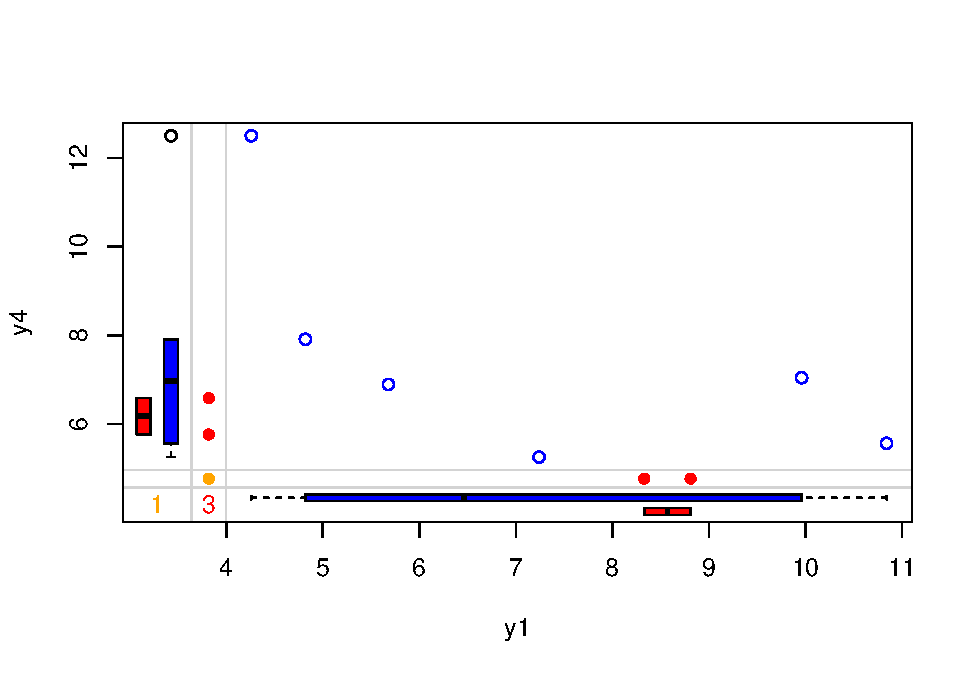
\includegraphics{03-descriptive-stat_files/figure-latex/unnamed-chunk-2-2.pdf}

\begin{Shaded}
\begin{Highlighting}[]
\CommentTok{\# Box{-}and{-}Whisker plot}
\FunctionTok{boxplot}\NormalTok{(count }\SpecialCharTok{\textasciitilde{}}\NormalTok{ spray, }\AttributeTok{data =}\NormalTok{ InsectSprays,}\AttributeTok{col =} \StringTok{"lightgray"}\NormalTok{,}\AttributeTok{main=}\StringTok{"boxplot"}\NormalTok{)}
\end{Highlighting}
\end{Shaded}

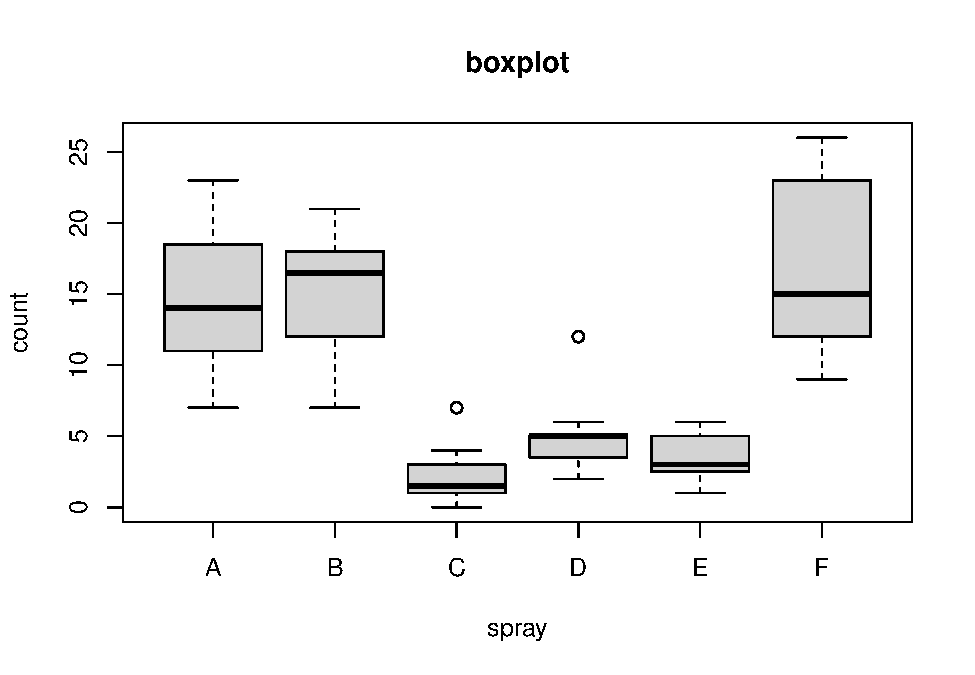
\includegraphics{03-descriptive-stat_files/figure-latex/unnamed-chunk-2-3.pdf}

\begin{Shaded}
\begin{Highlighting}[]
\CommentTok{\# Notched Boxplot}
\FunctionTok{boxplot}\NormalTok{(len}\SpecialCharTok{\textasciitilde{}}\NormalTok{supp}\SpecialCharTok{*}\NormalTok{dose, }\AttributeTok{data=}\NormalTok{ToothGrowth, }\AttributeTok{notch=}\ConstantTok{TRUE}\NormalTok{,}
  \AttributeTok{col=}\NormalTok{(}\FunctionTok{c}\NormalTok{(}\StringTok{"gold"}\NormalTok{,}\StringTok{"darkgreen"}\NormalTok{)),}
  \AttributeTok{main=}\StringTok{"Tooth Growth"}\NormalTok{, }\AttributeTok{xlab=}\StringTok{"Suppliment and Dose"}\NormalTok{)}
\end{Highlighting}
\end{Shaded}

\begin{verbatim}
## Warning in bxp(list(stats = structure(c(8.2, 9.7, 12.25, 16.5, 21.5, 4.2, : some
## notches went outside hinges ('box'): maybe set notch=FALSE
\end{verbatim}

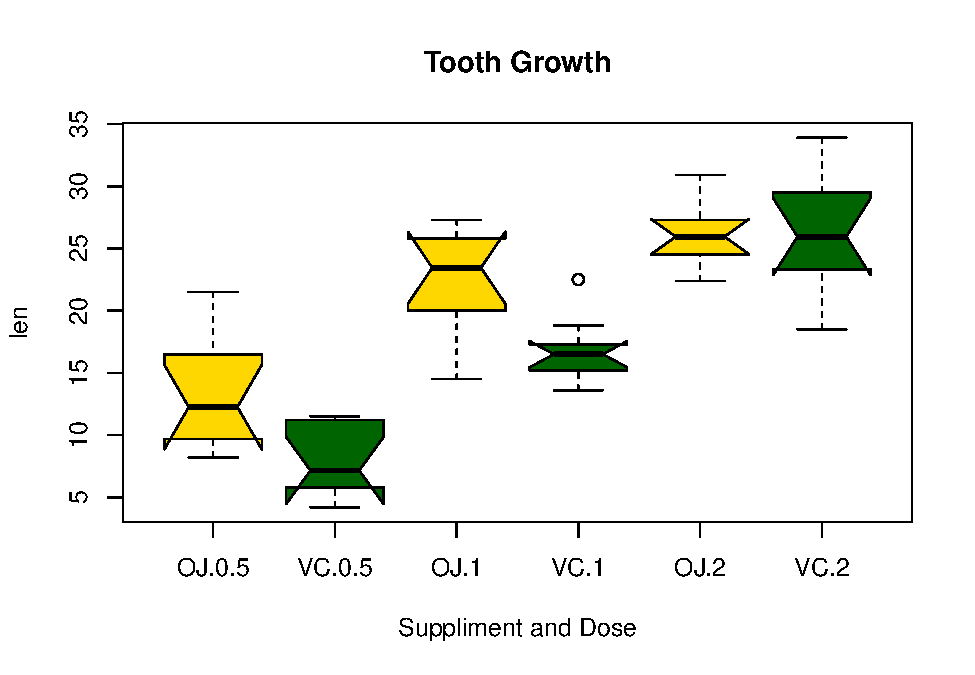
\includegraphics{03-descriptive-stat_files/figure-latex/unnamed-chunk-2-4.pdf}

\begin{Shaded}
\begin{Highlighting}[]
\CommentTok{\# If notches differ {-}\textgreater{} medians differ}

\CommentTok{\# Stem{-}and{-}Leaf Plots}
\FunctionTok{stem}\NormalTok{(data)}
\end{Highlighting}
\end{Shaded}

\begin{verbatim}
## 
##   The decimal point is at the |
## 
##   -2 | 65
##   -2 | 4
##   -1 | 97776665
##   -1 | 4433211
##   -0 | 99987777766666666655555
##   -0 | 4443333221110
##    0 | 001112222333444
##    0 | 555567778889999
##    1 | 0111224
##    1 | 5677889
##    2 | 14
\end{verbatim}

\begin{Shaded}
\begin{Highlighting}[]
\CommentTok{\# Bagplot {-} A 2D Boxplot Extension}
\NormalTok{pacman}\SpecialCharTok{::}\FunctionTok{p\_load}\NormalTok{(aplpack)}
\FunctionTok{attach}\NormalTok{(mtcars)}
\FunctionTok{bagplot}\NormalTok{(wt,mpg, }\AttributeTok{xlab=}\StringTok{"Car Weight"}\NormalTok{, }\AttributeTok{ylab=}\StringTok{"Miles Per Gallon"}\NormalTok{,}
  \AttributeTok{main=}\StringTok{"Bagplot Example"}\NormalTok{)}
\end{Highlighting}
\end{Shaded}

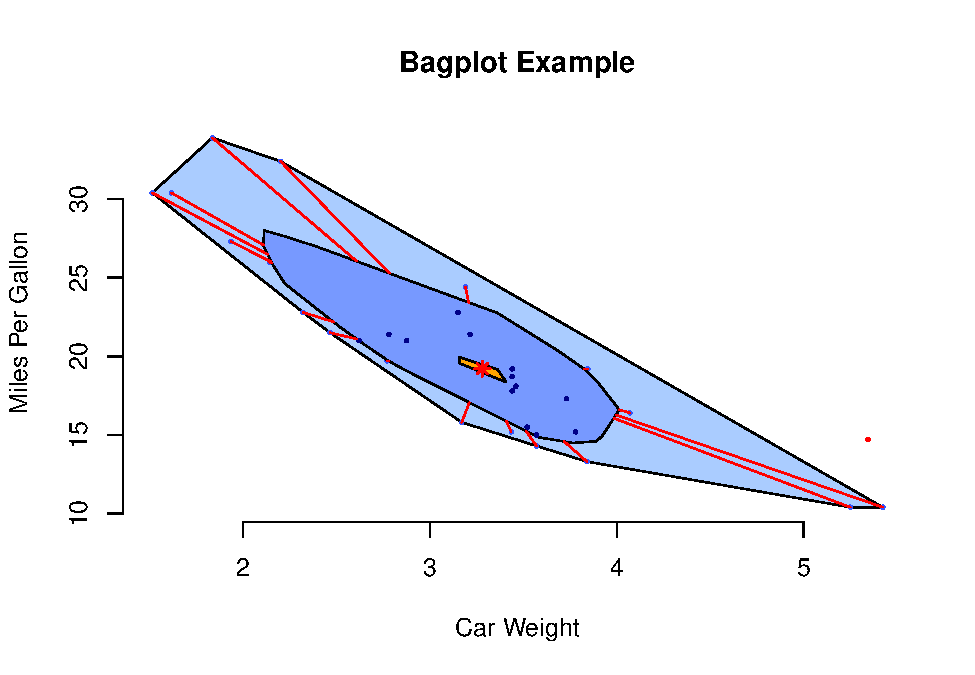
\includegraphics{03-descriptive-stat_files/figure-latex/unnamed-chunk-2-5.pdf}

Others more advanced plots

\begin{Shaded}
\begin{Highlighting}[]
\CommentTok{\# boxplot.matrix()  \#library("sfsmisc")}
\CommentTok{\# boxplot.n()       \#library("gplots")}
\CommentTok{\# vioplot()         \#library("vioplot")}
\end{Highlighting}
\end{Shaded}

\hypertarget{scatterplot}{%
\subsection{Scatterplot}\label{scatterplot}}

\begin{Shaded}
\begin{Highlighting}[]
\CommentTok{\# pairs(mtcars)}
\end{Highlighting}
\end{Shaded}

\hypertarget{normality-assessment}{%
\section{Normality Assessment}\label{normality-assessment}}

Since Normal (Gaussian) distribution has many applications, we typically want/ wish our data or our variable is normal. Hence, we have to assess the normality based on not only \protect\hyperlink{numerical-measures}{Numerical Measures} but also \protect\hyperlink{graphical-measures}{Graphical Measures}

\hypertarget{graphical-assessment}{%
\subsection{Graphical Assessment}\label{graphical-assessment}}

\begin{Shaded}
\begin{Highlighting}[]
\NormalTok{pacman}\SpecialCharTok{::}\FunctionTok{p\_load}\NormalTok{(}\StringTok{"car"}\NormalTok{)}
\FunctionTok{qqnorm}\NormalTok{(precip, }\AttributeTok{ylab =} \StringTok{"Precipitation [in/yr] for 70 US cities"}\NormalTok{)}
\FunctionTok{qqline}\NormalTok{(precip)}
\end{Highlighting}
\end{Shaded}

\includegraphics{03-descriptive-stat_files/figure-latex/unnamed-chunk-5-1.pdf}

The straight line represents the theoretical line for normally distributed data. The dots represent real empirical data that we are checking. If all the dots fall on the straight line, we can be confident that our data follow a normal distribution. If our data wiggle and deviate from the line, we should be concerned with the normality assumption.

\hypertarget{summary-statistics}{%
\subsection{Summary Statistics}\label{summary-statistics}}

Sometimes it's hard to tell whether your data follow the normal distribution by just looking at the graph. Hence, we often have to conduct statistical test to aid our decision. Common tests are

\begin{itemize}
\item
  \protect\hyperlink{methods-based-on-normal-probability-plot}{Methods based on normal probability plot}

  \begin{itemize}
  \tightlist
  \item
    \protect\hyperlink{correlation-coefficient-with-normal-probability-plots}{Correlation Coefficient with Normal Probability Plots}\\
  \item
    \protect\hyperlink{shapiro-wilk-test}{Shapiro-Wilk Test}\\
  \end{itemize}
\item
  \protect\hyperlink{methods-based-on-empirical-cumulative-distribution-function}{Methods based on empirical cumulative distribution function}

  \begin{itemize}
  \tightlist
  \item
    \protect\hyperlink{anderson-darling-test}{Anderson-Darling Test}\\
  \item
    \protect\hyperlink{kolmogorov-smirnov-test}{Kolmogorov-Smirnov Test}\\
  \item
    \protect\hyperlink{cramer-von-mises-test}{Cramer-von Mises Test}
  \item
    \protect\hyperlink{jarquebera-test}{Jarque--Bera Test}
  \end{itemize}
\end{itemize}

\hypertarget{methods-based-on-normal-probability-plot}{%
\subsubsection{Methods based on normal probability plot}\label{methods-based-on-normal-probability-plot}}

\hypertarget{correlation-coefficient-with-normal-probability-plots}{%
\paragraph{Correlation Coefficient with Normal Probability Plots}\label{correlation-coefficient-with-normal-probability-plots}}

\citep{Looney_1985} \citep{Shapiro_1972} The correlation coefficient between \(y_{(i)}\) and \(m_i^*\) as given on the normal probability plot:

\[W^*=\frac{\sum_{i=1}^{n}(y_{(i)}-\bar{y})(m_i^*-0)}{(\sum_{i=1}^{n}(y_{(i)}-\bar{y})^2\sum_{i=1}^{n}(m_i^*-0)^2)^.5}\]

where \(\bar{m^*}=0\)

Pearson product moment formula for correlation:

\[\hat{p}=\frac{\sum_{i-1}^{n}(y_i-\bar{y})(x_i-\bar{x})}{(\sum_{i=1}^{n}(y_{i}-\bar{y})^2\sum_{i=1}^{n}(x_i-\bar{x})^2)^.5}\]

\begin{itemize}
\tightlist
\item
  When the correlation is 1, the plot is exactly linear and normality is assumed.
\item
  The closer the correlation is to zero, the more confident we are to reject normality
\item
  Inference on W* needs to be based on special tables \citep{Looney_1985}
\end{itemize}

\begin{Shaded}
\begin{Highlighting}[]
\FunctionTok{library}\NormalTok{(}\StringTok{"EnvStats"}\NormalTok{)}
\end{Highlighting}
\end{Shaded}

\begin{verbatim}
## 
## Attaching package: 'EnvStats'
\end{verbatim}

\begin{verbatim}
## The following object is masked from 'package:car':
## 
##     qqPlot
\end{verbatim}

\begin{verbatim}
## The following objects are masked from 'package:e1071':
## 
##     kurtosis, skewness
\end{verbatim}

\begin{verbatim}
## The following objects are masked from 'package:stats':
## 
##     predict, predict.lm
\end{verbatim}

\begin{verbatim}
## The following object is masked from 'package:base':
## 
##     print.default
\end{verbatim}

\begin{Shaded}
\begin{Highlighting}[]
\FunctionTok{gofTest}\NormalTok{(data,}\AttributeTok{test=}\StringTok{"ppcc"}\NormalTok{)}\SpecialCharTok{$}\NormalTok{p.value }\CommentTok{\#Probability Plot Correlation Coefficient }
\end{Highlighting}
\end{Shaded}

\begin{verbatim}
## [1] 0.8235111
\end{verbatim}

\hypertarget{shapiro-wilk-test}{%
\paragraph{Shapiro-Wilk Test}\label{shapiro-wilk-test}}

\citep{Shapiro_1965}

\[W=(\frac{\sum_{i=1}^{n}a_i(y_{(i)}-\bar{y})(m_i^*-0)}{(\sum_{i=1}^{n}a_i^2(y_{(i)}-\bar{y})^2\sum_{i=1}^{n}(m_i^*-0)^2)^.5})^2\]

where \(a_1,..,a_n\) are weights computed from the covariance matrix for the order statistics.

\begin{itemize}
\tightlist
\item
  Researchers typically use this test to assess normality. (n \textless{} 2000) Under normality, W is close to 1, just like \(W^*\). Notice that the only difference between W and W* is the ``weights''.
\end{itemize}

\begin{Shaded}
\begin{Highlighting}[]
\FunctionTok{gofTest}\NormalTok{(data,}\AttributeTok{test=}\StringTok{"sw"}\NormalTok{)}\SpecialCharTok{$}\NormalTok{p.value }\CommentTok{\#Shapiro{-}Wilk is the default.}
\end{Highlighting}
\end{Shaded}

\begin{verbatim}
## [1] 0.711287
\end{verbatim}

\hypertarget{methods-based-on-empirical-cumulative-distribution-function}{%
\subsubsection{Methods based on empirical cumulative distribution function}\label{methods-based-on-empirical-cumulative-distribution-function}}

The formula for the empirical cumulative distribution function (CDF) is:

\(F_n(t)\) = estimate of probability that an observation \(\le\) t = (number of observation \(\le\) t)/n

This method requires large sample sizes. However, it can apply to distributions other than the normal (Gaussian) one.

\begin{Shaded}
\begin{Highlighting}[]
\CommentTok{\# Empirical CDF hand{-}code}
\FunctionTok{plot.ecdf}\NormalTok{(data,}\AttributeTok{verticals =}\NormalTok{ T, }\AttributeTok{do.points=}\NormalTok{F)}
\end{Highlighting}
\end{Shaded}

\includegraphics{03-descriptive-stat_files/figure-latex/unnamed-chunk-8-1.pdf}

\hypertarget{anderson-darling-test}{%
\paragraph{Anderson-Darling Test}\label{anderson-darling-test}}

\citep{Anderson_1952}

The Anderson-Darling statistic:

\[A^2=\int_{-\infty}^{\infty}(F_n(t)=F(t))^2\frac{dF(t)}{F(t)(1-F(t))}\]

\begin{itemize}
\tightlist
\item
  a weight average of squared deviations (it weights small and large values of t more)
\end{itemize}

For the normal distribution,

\(A^2 = - (\sum_{i=1}^{n}(2i-1)(ln(p_i) +ln(1-p_{n+1-i}))/n-n\)

where \(p_i=\Phi(\frac{y_{(i)}-\bar{y}}{s})\), the probability that a standard normal variable is less than \(\frac{y_{(i)}-\bar{y}}{s}\)

\begin{itemize}
\item
  Reject normal assumption when \(A^2\) is too large
\item
  Evaluate the null hypothesis that the observations are randomly selected from a normal population based on the critical value provided by \citep{Marsaglia_2004} and \citep{Stephens_1974}
\item
  This test can be applied to other distributions:

  \begin{itemize}
  \tightlist
  \item
    Exponential
  \item
    Logistic
  \item
    Gumbel
  \item
    Extreme-value
  \item
    Weibull: log(Weibull) = Gumbel
  \item
    Gamma
  \item
    Logistic
  \item
    Cauchy
  \item
    von Mises
  \item
    Log-normal (two-parameter)
  \end{itemize}
\end{itemize}

Consult \citep{Stephens_1974} for more detailed transformation and critical values.

\begin{Shaded}
\begin{Highlighting}[]
\FunctionTok{gofTest}\NormalTok{(data,}\AttributeTok{test=}\StringTok{"ad"}\NormalTok{)}\SpecialCharTok{$}\NormalTok{p.value }\CommentTok{\#Anderson{-}Darling}
\end{Highlighting}
\end{Shaded}

\begin{verbatim}
## [1] 0.6570096
\end{verbatim}

\hypertarget{kolmogorov-smirnov-test}{%
\paragraph{Kolmogorov-Smirnov Test}\label{kolmogorov-smirnov-test}}

\begin{itemize}
\tightlist
\item
  Based on the largest absolute difference between empirical and expected cumulative distribution
\item
  Another deviation of K-S test is Kuiper's test
\end{itemize}

\begin{Shaded}
\begin{Highlighting}[]
\FunctionTok{gofTest}\NormalTok{(data,}\AttributeTok{test=}\StringTok{"ks"}\NormalTok{)}\SpecialCharTok{$}\NormalTok{p.value }\CommentTok{\#Komogorov{-}Smirnov }
\end{Highlighting}
\end{Shaded}

\begin{verbatim}
## Warning in ksGofTest(x = c(0.366710433093215, -0.578925793462227, -0.523624011578963, : The standard Kolmogorov-Smirnov test is very conservative (Type I error smaller than assumed; high Type II error) for testing departures from the Normal distribution when you have to estimate the distribution parameters.
\end{verbatim}

\begin{verbatim}
## [1] 0.7655141
\end{verbatim}

\hypertarget{cramer-von-mises-test}{%
\paragraph{Cramer-von Mises Test}\label{cramer-von-mises-test}}

\begin{itemize}
\tightlist
\item
  Based on the average squared discrepancy between the empirical distribution and a given theoretical distribution. Each discrepancy is weighted equally (unlike Anderson-Darling test weights end points more heavily)
\end{itemize}

\begin{Shaded}
\begin{Highlighting}[]
\FunctionTok{gofTest}\NormalTok{(data,}\AttributeTok{test=}\StringTok{"cvm"}\NormalTok{)}\SpecialCharTok{$}\NormalTok{p.value }\CommentTok{\#Cramer{-}von Mises}
\end{Highlighting}
\end{Shaded}

\begin{verbatim}
## [1] 0.5545067
\end{verbatim}

\hypertarget{jarquebera-test}{%
\paragraph{Jarque--Bera Test}\label{jarquebera-test}}

\citep{Bera_1981}

Based on the skewness and kurtosis to test normality.

\(JB = \frac{n}{6}(S^2+(K-3)^2/4)\) where S is the sample skewness and K is the sample kurtosis

\(S=\frac{\hat{\mu_3}}{\hat{\sigma}^3}=\frac{\sum_{i=1}^{n}(x_i-\bar{x})^3/n}{(\sum_{i=1}^{n}(x_i-\bar{x})^2/n)^\frac{3}{2}}\)

\(K=\frac{\hat{\mu_4}}{\hat{\sigma}^4}=\frac{\sum_{i=1}^{n}(x_i-\bar{x})^4/n}{(\sum_{i=1}^{n}(x_i-\bar{x})^2/n)^2}\)

recall \(\hat{\sigma^2}\) is the estimate of the second central moment (variance) \(\hat{\mu_3}\) and \(\hat{\mu_4}\) are the estimates of third and fourth central moments.

If the data comes from a normal distribution, the JB statistic asymptotically has a chi-squared distribution with two degrees of freedom.

The null hypothesis is a joint hypothesis of the skewness being zero and the excess kurtosis being zero.

\hypertarget{basic-statistical-inference}{%
\chapter{Basic Statistical Inference}\label{basic-statistical-inference}}

\begin{itemize}
\tightlist
\item
  \protect\hyperlink{one-sample-inference}{One Sample Inference}\\
\item
  \protect\hyperlink{two-sample-inference}{Two Sample Inference}\\
\item
  \protect\hyperlink{categorical-data-analysis}{Categorical Data Analysis}
\end{itemize}

\begin{itemize}
\tightlist
\item
  Make \textbf{inferences} (an interpretation) about the true parameter value \(\beta\) based on our estimator/estimate
\item
  Test whether our underlying assumptions (about the true population parameters, random variables, or model specification) hold true.
\end{itemize}

Testing does not

\begin{itemize}
\tightlist
\item
  Confirm with 100\% a hypothesis is true
\item
  Confirm with 100\% a hypothesis is false
\item
  Tell you how to interpret the estimate value (Economic vs.~Practical vs.~Statistical Significance)
\end{itemize}

Hypothesis: Translate an objective in better understanding the results in terms of specifying a value (or sets of values) in which our population parameters should/should not lie.

\begin{itemize}
\tightlist
\item
  \textbf{Null hypothesis} (\(H_0\)): A statement about the population parameter that we take to be true in which we would need the data to provide substantial evidence that against it.

  \begin{itemize}
  \tightlist
  \item
    Can be either a single value (ex: \(H_0: \beta=0\)) or a set of values (ex: \(H_0: \beta_1 \ge 0\))
  \item
    Will generally be the value you would not like the population parameter to be (subjective)

    \begin{itemize}
    \tightlist
    \item
      \(H_0: \beta_1=0\) means you would like to see a non-zero coefficient
    \item
      \(H_0: \beta_1 \ge 0\) means you would like to see a negative effect
    \end{itemize}
  \item
    ``Test of Significance'' refers to the two-sided test: \(H_0: \beta_j=0\)
  \end{itemize}
\item
  \textbf{Alternative hypothesis} (\(H_a\) or \(H_1\)) (Research Hypothesis): All other possible values that the population parameter may be if the null hypothesis does not hold.
\end{itemize}

\textbf{Type I Error}

Error made when \(H_0\) is rejected when, in fact, \(H_0\) is true.\\
The probability of committing a Type I error is \(\alpha\) (known as \textbf{level of significance} of the test)

Type I error (\(\alpha\)): probability of rejecting \(H_0\) when it is true.

Legal analogy: In U.S. law, a defendant is presumed to be ``innocent until proven guilty''.\\
If the null hypothesis is that a person is innocent, the Type I error is the probability that you conclude the person is guilty when he is innocent.

\textbf{Type II Error}

Type II error level (\(\beta\)): probability that you fail to reject the null hypothesis when it is false.

In the legal analogy, this is the probability that you fail to find the person guilty when he or she is guilty.

Error made when \(H_0\) is not rejected when, in fact, \(H_1\) is true\\
The probability of committing a Type II error is \(\beta\) (known as the \textbf{power} of the test)

Random sample of size n: A collection of n independent random variables taken from the distribution X, each with the same distribution as X.

\textbf{Sample mean}

\[
\bar{X}= (\sum_{i=1}^{n}X_i)/n
\]

\textbf{Sample Median}

\(\tilde{x}\) = the middle observation in a sample of observation order from smallest to largest (or vice versa).

If n is odd, \(\tilde{x}\) is the middle observation,\\
If n is even, \(\tilde{x}\) is the average of the two middle observations.

\textbf{Sample variance}
\[
S^2 = \frac{\sum_{i=1}^{n}(X_i = \bar{X})^2}{n-1}= \frac{n\sum_{i=1}^{n}X_i^2 -(\sum_{i=1}^{n}X_i)^2}{n(n-1)}
\]

\textbf{Sample standard deviation}
\[
S = \sqrt{S^2}
\]

\textbf{Sample proportions}
\[
\hat{p} = \frac{X}{n} = \frac{\text{number in the sample with trait}}{\text{sample size}}
\]

\[
\widehat{p_1-p_2} = \hat{p_1}-\hat{p_2} = \frac{X_1}{n_1} - \frac{X_2}{n_2} = \frac{n_2X_1 = n_1X_2}{n_1n_2}
\]

\textbf{Estimators}\\
\textbf{Point Estimator}\\
\(\hat{\theta}\) is a statistic used to approximate a population parameter \(\theta\)

\textbf{Point estimate}\\
The numerical value assumed by \(\hat{\theta}\) when evaluated for a given sample

\textbf{Unbiased estimator}\\
If \(E(\hat{\theta}) = \theta\), then \(\hat{\theta}\) is an unbiased estimator for \(\theta\)

\begin{enumerate}
\def\labelenumi{\arabic{enumi}.}
\tightlist
\item
  \(\bar{X}\) is an unbiased estimator for \(\mu\)
\item
  \(S^2\) is an unbiased estimator for \(\sigma^2\)
\item
  \(\hat{p}\) is an unbiased estimator for p
\item
  \(\widehat{p_1-P_2}\) is an unbiased estimator for \(p_1- p_2\)
\item
  \(\bar{X_1} - \bar{X_2}\) is an unbiased estimator for \(\mu_1 - \mu_2\)
\end{enumerate}

\textbf{Note}: \(S\) is a biased estimator for \(\sigma\)

\textbf{Distribution of the sample mean}

If \(\bar{X}\) is the sample mean based on a random sample of size n drawn from a normal distribution X with mean \(\mu\) and standard deviation \(\sigma\), the \(\bar{X}\) is normally distributed, with mean \(\mu_{\bar{X}} = \mu\) and variance \(\sigma_{\bar{X}}^2 = Var(\bar{X}) = \frac{\sigma^2}{n}\). Then the \textbf{standard error of the mean} is: \(\sigma_{\bar{X}}= \frac{\sigma}{\sqrt{n}}\)

\hypertarget{one-sample-inference}{%
\section{One Sample Inference}\label{one-sample-inference}}

\(Y_i \sim i.i.d. N(\mu, \sigma^2)\)

i.i.d. standards for ``independent and identically distributed''

Hence, we have the following model:

\(Y_i=\mu +\epsilon_i\) where

\begin{itemize}
\tightlist
\item
  \(\epsilon_i \sim^{iid} N(0,\sigma^2)\)\\
\item
  \(E(Y_i)=\mu\)\\
\item
  \(Var(Y_i)=\sigma^2\)\\
\item
  \(\bar{y} \sim N(\mu,\sigma^2/n)\)
\end{itemize}

\hypertarget{the-mean}{%
\subsection{The Mean}\label{the-mean}}

When \(\sigma^2\) is estimated by \(s^2\), then

\[
\frac{\bar{y}-\mu}{s/\sqrt{n}} \sim t_{n-1}
\]

Then, a \(100(1-\alpha) \%\) confidence interval for \(\mu\) is obtained from:

\[
1 - \alpha = P(-t_{\alpha/2;n-1} \le \frac{\bar{y}-\mu}{s/\sqrt{n}} \le t_{\alpha/2;n-1}) \\
= P(\bar{y} - (t_{\alpha/2;n-1})s/\sqrt{n} \le \mu \le \bar{y} + (t_{\alpha/2;n-1})s/\sqrt{n})
\]

And the interval is

\[
\bar{y} \pm (t_{\alpha/2;n-1})s/\sqrt{n}
\]

and \(s/\sqrt{n}\) is the standard error of \(\bar{y}\)

If the experiment were repeated many times, \(100(1-\alpha) \%\) of these intervals would contain \(\mu\)

\begin{longtable}[]{@{}llll@{}}
\toprule
\begin{minipage}[b]{(\columnwidth - 3\tabcolsep) * \real{0.25}}\raggedright
\strut
\end{minipage} & \begin{minipage}[b]{(\columnwidth - 3\tabcolsep) * \real{0.25}}\raggedright
Confidence Interval \(100(1-\alpha)%
\)\strut
\end{minipage} & \begin{minipage}[b]{(\columnwidth - 3\tabcolsep) * \real{0.25}}\raggedright
Sample Sizes Confidence \(\alpha\), Error d\strut
\end{minipage} & \begin{minipage}[b]{(\columnwidth - 3\tabcolsep) * \real{0.25}}\raggedright
Hypothesis Testing Test Statistic\strut
\end{minipage}\tabularnewline
\midrule
\endhead
\begin{minipage}[t]{(\columnwidth - 3\tabcolsep) * \real{0.25}}\raggedright
When \(\sigma^2\) is known, X is normal (or \(n \ge 25\))\strut
\end{minipage} & \begin{minipage}[t]{(\columnwidth - 3\tabcolsep) * \real{0.25}}\raggedright
\(\bar{X} \pm z_{\alpha/2}\frac{\sigma}{\sqrt{n}}\)\strut
\end{minipage} & \begin{minipage}[t]{(\columnwidth - 3\tabcolsep) * \real{0.25}}\raggedright
\(n \approx \frac{z_{\alpha/2}^2 \sigma^2}{d^2}\)\strut
\end{minipage} & \begin{minipage}[t]{(\columnwidth - 3\tabcolsep) * \real{0.25}}\raggedright
\(z = \frac{\bar{X}-\mu_0}{\sigma/\sqrt{n}}\)\strut
\end{minipage}\tabularnewline
\begin{minipage}[t]{(\columnwidth - 3\tabcolsep) * \real{0.25}}\raggedright
When \(\sigma^2\) is unknown, X is normal (or \(n \ge 25\))\strut
\end{minipage} & \begin{minipage}[t]{(\columnwidth - 3\tabcolsep) * \real{0.25}}\raggedright
\(\bar{X} \pm t_{\alpha/2}\frac{s}{\sqrt{n}}\)\strut
\end{minipage} & \begin{minipage}[t]{(\columnwidth - 3\tabcolsep) * \real{0.25}}\raggedright
\(n \approx \frac{z_{\alpha/2}^2 s^2}{d^2}\)\strut
\end{minipage} & \begin{minipage}[t]{(\columnwidth - 3\tabcolsep) * \real{0.25}}\raggedright
\(t = \frac{\bar{X}-\mu_0}{s/\sqrt{n}}\)\strut
\end{minipage}\tabularnewline
\bottomrule
\end{longtable}

\hypertarget{for-difference-of-means-mu_1-mu_2-independent-samples}{%
\subsubsection{\texorpdfstring{For Difference of Means (\(\mu_1-\mu_2\)), Independent Samples}{For Difference of Means (\textbackslash mu\_1-\textbackslash mu\_2), Independent Samples}}\label{for-difference-of-means-mu_1-mu_2-independent-samples}}

\begin{longtable}[]{@{}llll@{}}
\toprule
\begin{minipage}[b]{(\columnwidth - 3\tabcolsep) * \real{0.25}}\raggedright
\strut
\end{minipage} & \begin{minipage}[b]{(\columnwidth - 3\tabcolsep) * \real{0.25}}\raggedright
\(100(1-\alpha)%
\) Confidence Interval\strut
\end{minipage} & \begin{minipage}[b]{(\columnwidth - 3\tabcolsep) * \real{0.25}}\raggedright
Hypothesis Testing Test Statistic\strut
\end{minipage} & \begin{minipage}[b]{(\columnwidth - 3\tabcolsep) * \real{0.25}}\raggedright
\strut
\end{minipage}\tabularnewline
\midrule
\endhead
\begin{minipage}[t]{(\columnwidth - 3\tabcolsep) * \real{0.25}}\raggedright
When \(\sigma^2\) is known\strut
\end{minipage} & \begin{minipage}[t]{(\columnwidth - 3\tabcolsep) * \real{0.25}}\raggedright
\(\bar{X}_1 - \bar{X}_2 \pm z_{\alpha/2}\sqrt{\frac{\sigma^2_1}{n_1}+\frac{\sigma^2_2}{n_2}}\)\strut
\end{minipage} & \begin{minipage}[t]{(\columnwidth - 3\tabcolsep) * \real{0.25}}\raggedright
\(z= \frac{(\bar{X}_1-\bar{X}_2)-(\mu_1-\mu_2)_0}{\sqrt{\frac{\sigma^2_1}{n_1}+\frac{\sigma^2_2}{n_2}}}\)\strut
\end{minipage} & \begin{minipage}[t]{(\columnwidth - 3\tabcolsep) * \real{0.25}}\raggedright
\strut
\end{minipage}\tabularnewline
\begin{minipage}[t]{(\columnwidth - 3\tabcolsep) * \real{0.25}}\raggedright
When \(\sigma^2\) is unknown, Variances Assumed EQUAL\strut
\end{minipage} & \begin{minipage}[t]{(\columnwidth - 3\tabcolsep) * \real{0.25}}\raggedright
\(\bar{X}_1 - \bar{X}_2 \pm t_{\alpha/2}\sqrt{s^2_p(\frac{1}{n_1}+\frac{1}{n_2})}\)\strut
\end{minipage} & \begin{minipage}[t]{(\columnwidth - 3\tabcolsep) * \real{0.25}}\raggedright
\(t = \frac{(\bar{X}_1-\bar{X}_2)-(\mu_1-\mu_2)_0}{\sqrt{s^2_p(\frac{1}{n_1}+\frac{1}{n_2})}}\)\strut
\end{minipage} & \begin{minipage}[t]{(\columnwidth - 3\tabcolsep) * \real{0.25}}\raggedright
Pooled Variance: \(s_p^2 = \frac{(n_1 -1)s^2_1 - (n_2-1)s^2_2}{n_1 + n_2 -2}\) Degrees of Freedom: \(\gamma = n_1 + n_2 -2\)\strut
\end{minipage}\tabularnewline
\begin{minipage}[t]{(\columnwidth - 3\tabcolsep) * \real{0.25}}\raggedright
When \(\sigma^2\) is unknown, Variances Assumed UNEQUAL\strut
\end{minipage} & \begin{minipage}[t]{(\columnwidth - 3\tabcolsep) * \real{0.25}}\raggedright
\(\bar{X}_1 - \bar{X}_2 \pm t_{\alpha/2}\sqrt{(\frac{s^2_1}{n_1}+\frac{s^2_2}{n_2})}\)\strut
\end{minipage} & \begin{minipage}[t]{(\columnwidth - 3\tabcolsep) * \real{0.25}}\raggedright
\(t = \frac{(\bar{X}_1-\bar{X}_2)-(\mu_1-\mu_2)_0}{\sqrt{(\frac{s^2_1}{n_1}+\frac{s^2_2}{n_2})}}\)\strut
\end{minipage} & \begin{minipage}[t]{(\columnwidth - 3\tabcolsep) * \real{0.25}}\raggedright
Degrees of Freedom: \(\gamma = \frac{(\frac{s_1^2}{n_1}+\frac{s^2_2}{n_2})^2}{\frac{(\frac{s_1^2}{n_1})^2}{n_1-1}+\frac{(\frac{s_2^2}{n_2})^2}{n_2-1}}\)\strut
\end{minipage}\tabularnewline
\bottomrule
\end{longtable}

\hypertarget{for-difference-of-means-mu_1---mu_2-paired-samples-d-x-y}{%
\subsubsection{\texorpdfstring{For Difference of Means (\(\mu_1 - \mu_2\)), Paired Samples (D = X-Y)}{For Difference of Means (\textbackslash mu\_1 - \textbackslash mu\_2), Paired Samples (D = X-Y)}}\label{for-difference-of-means-mu_1---mu_2-paired-samples-d-x-y}}

\textbf{\(100(1-\alpha)%
\) Confidence Interval}\\
\[
\bar{D} \pm t_{\alpha/2}\frac{s_d}{\sqrt{n}}
\]

\textbf{Hypothesis Testing Test Statistic}

\[
t = \frac{\bar{D}-D_0}{s_d / \sqrt{n}}
\]

\hypertarget{difference-of-two-proprotions}{%
\subsubsection{Difference of Two Proprotions}\label{difference-of-two-proprotions}}

\textbf{Mean}

\[
\hat{p_1}-\hat{p_2}
\]

\textbf{Variance}
\[
\frac{p_1(1-p_1)}{n_1} + \frac{p_2(1-p_2)}{n_2}
\]

\textbf{\(100(1-\alpha)%
\) Confidence Interval}

\[
\hat{p_1}-\hat{p_2} + z_{\alpha/2}\sqrt{\frac{p_1(1-p_1)}{n_1} + \frac{p_2(1-p_2)}{n_2}}
\]

\textbf{Sample Sizes, Confidence \(\alpha\), Error d}\\
(Prior Estimate fo \(\hat{p_1},\hat{p_2}\))

\[
n \approx \frac{z_{\alpha/2}^2[p_1(1-p_1)+p_2(1-p_2)]}{d^2}
\]

(No Prior Estimates for \(\hat{p}\))

\[
n \approx \frac{z_{\alpha/2}^2}{2d^2}
\]

\textbf{Hypothesis Testing - Test Statistics}

Null Value \((p_1 - p_2) \neq 0\)

\[
z = \frac{(\hat{p_1} - \hat{p_2})-(p_1 - p_2)_0}{\sqrt{\frac{p_1(1-p_1)}{n_1} + \frac{p_2(1-p_2)}{n_2}}}
\]

Null Value \((p_1 - p_2)_0 = 0\)

\[
z = \frac{\hat{p_1} - \hat{p_2}}{\sqrt{\hat{p}(1-\hat{p})(\frac{1}{n_1}+\frac{1}{n_2})}}
\]

where

\[
\hat{p}= \frac{x_1 + x_2}{n_1 + n_2} = \frac{n_1 \hat{p_1} + n_2 \hat{p_2}}{n_1 + n_2}
\]

\hypertarget{single-variance}{%
\subsection{Single Variance}\label{single-variance}}

\[
1 - \alpha = P( \chi_{1-\alpha/2;n-1}^2) \le (n-1)s^2/\sigma^2 \le \chi_{\alpha/2;n-1}^2) \\
= P(\frac{(n-1)s^2}{\chi_{\alpha/2}^2} \le \sigma^2 \le \frac{(n-1)s^2}{\chi_{1-\alpha/2}^2})
\]

and a \(100(1-\alpha) \%\) confidence interval for \(\sigma^2\) is:

\[
(\frac{(n-1)s^2}{\chi_{\alpha/2;n-1}^2},\frac{(n-1)s^2}{\chi_{1-\alpha/2;n-1}^2})
\]
Confidence limits for \(\sigma^2\) are obtained by computing the positive square roots of these limits

Equivalently,

\textbf{\(100(1-\alpha)%
\) Confidence Interval}

\[
L_1 = \frac{(n-1)s^2}{\chi^2_{\alpha/2}} \\
L_1 = \frac{(n-1)s^2}{\chi^2_{1-\alpha/2}}
\]
\textbf{Hypothesis Testing Test Statistic}

\[
\chi^2 = \frac{(n-1)s^2}{\sigma^2_0}
\]

\hypertarget{single-proportion-p}{%
\subsection{Single Proportion (p)}\label{single-proportion-p}}

\begin{longtable}[]{@{}llll@{}}
\toprule
\begin{minipage}[b]{(\columnwidth - 3\tabcolsep) * \real{0.25}}\raggedright
Confidence Interval \(100(1-\alpha)%
\)\strut
\end{minipage} & \begin{minipage}[b]{(\columnwidth - 3\tabcolsep) * \real{0.25}}\raggedright
Sample Sizes Confidence \(\alpha\), Error d (prior estimate for \(\hat{p}\))\strut
\end{minipage} & \begin{minipage}[b]{(\columnwidth - 3\tabcolsep) * \real{0.25}}\raggedright
(No prior estimate for \(\hat{p}\))\strut
\end{minipage} & \begin{minipage}[b]{(\columnwidth - 3\tabcolsep) * \real{0.25}}\raggedright
Hypothesis Testing Test Statistic\strut
\end{minipage}\tabularnewline
\midrule
\endhead
\begin{minipage}[t]{(\columnwidth - 3\tabcolsep) * \real{0.25}}\raggedright
\(\hat{p} \pm z_{\alpha/2}\sqrt{\frac{\hat{p}(1-\hat{p})}{n}}\)\strut
\end{minipage} & \begin{minipage}[t]{(\columnwidth - 3\tabcolsep) * \real{0.25}}\raggedright
\(n \approx \frac{z_{\alpha/2}^2 \hat{p}(1-\hat{p})}{d^2}\)\strut
\end{minipage} & \begin{minipage}[t]{(\columnwidth - 3\tabcolsep) * \real{0.25}}\raggedright
\(n \approx \frac{z_{\alpha/2}^2}{4d^2}\)\strut
\end{minipage} & \begin{minipage}[t]{(\columnwidth - 3\tabcolsep) * \real{0.25}}\raggedright
\(z = \frac{\hat{p}-p_0}{\sqrt{\frac{p_0(1-p_0)}{n}}}\)\strut
\end{minipage}\tabularnewline
\bottomrule
\end{longtable}

\hypertarget{power}{%
\subsection{Power}\label{power}}

Formally, power (for the test of the mean) is given by:

\[
\pi(\mu) = 1 - \beta = P(\text{test rejects } H_0|\mu)
\]
To evaluate the power, one needs to know the distribution of the test statistic if the null hypothesis is false.

For 1-sided z-test where \(H_0: \mu \le \mu_0 \\ H_A: \mu >0\)

The power is:

\[
\begin{aligned}
\pi(\mu) &= P(\bar{y} > \mu_0 + z_{\alpha} \sigma/\sqrt{n}|\mu) \\
&= P(Z = \frac{\bar{y} - \mu}{\sigma / \sqrt{n}} > z_{\alpha} + \frac{\mu_0 - \mu}{\sigma/ \sqrt{n}}|\mu) \\
&= 1 - \Phi(z_{\alpha} + \frac{(\mu_0 - \mu)\sqrt{n}}{\sigma}) \\
&= \Phi(-z_{\alpha}+\frac{(\mu -\mu_0)\sqrt{n}}{\sigma})
\end{aligned}
\]

where \(1-\Phi(x) = \Phi(-x)\) since the normal pdf is symmetric

Power is correlated to the difference in \(\mu - \mu_0\), sample size n, variance \(\sigma^2\), and the \(\alpha\)-level of the test (through \(z_{\alpha}\))\\
Equivalently, power can be increased by making \(\alpha\) large, \(\sigma^2\) smaller, or n larger.

For 2-sided z-test is:

\[
\pi(\mu) = \Phi(-z_{\alpha/2} + \frac{(\mu_0 - \mu)\sqrt{n}}{\sigma}) + \Phi(-z_{\alpha/2}+\frac{(\mu - \mu_0)\sqrt{n}}{\sigma})
\]

\hypertarget{sample-size}{%
\subsection{Sample Size}\label{sample-size}}

\hypertarget{sided-z-test}{%
\subsubsection{1-sided Z-test}\label{sided-z-test}}

Example: to show that the mean response \(\mu\) under the treatment is higher than the mean response \(\mu_0\) without treatment (show that the treatment effect \(\delta = \mu -\mu_0\) is large)

Because power is an increasing function of \(\mu - \mu_0\), it is only necessary to find n that makes the power equal to \(1- \beta\) at \(\mu = \mu_0 + \delta\)

Hence, we have

\[
\pi(\mu_0 + \delta) = \Phi(-z_{\alpha} + \frac{\delta \sqrt{n}}{\sigma}) = 1 - \beta
\]

Since \(\Phi (z_{\beta})= 1-\beta\), we have

\[
-z_{\alpha} + \frac{\delta \sqrt{n}}{\sigma} = z_{\beta}
\]

Then n is

\[
n = (\frac{(z_{\alpha}+z_{\beta})\sigma}{\delta})^2
\]

Then, we need larger samples, when

\begin{itemize}
\tightlist
\item
  the sample variability is large (\(\sigma\) is large)
\item
  \(\alpha\) is small (\(z_{\alpha}\) is large)
\item
  power \(1-\beta\) is large (\(z_{\beta}\) is large)
\item
  The magnitude of the effect is smaller (\(\delta\) is small)
\end{itemize}

Since we don't know \(\delta\) and \(\sigma\). We can base \(\sigma\) on previous studies, pilot studies. Or, obtain an estimate of \(\sigma\) by anticipating the range of the observation (without outliers). divide this range by 4 and use the resulting number as an approximate estimate of \(\sigma\). For normal (distribution) data, this is reasonable.

\hypertarget{sided-z-test-1}{%
\subsubsection{2-sided Z-test}\label{sided-z-test-1}}

We want to know the min n, required to guarantee \(1-\beta\) power when the treatment effect \(\delta = |\mu - \mu_0|\) is at least greater than 0. Since the power function for the 2-sided is increasing and symmetric in \(|\mu - \mu_0|\), we only need to find n that makes the power equal to \(1-\beta\) when \(\mu = \mu_0 + \delta\)

\[
n = (\frac{(z_{\alpha/2} + z_{\beta}) \sigma}{\delta})^2
\]

We could also use the confidence interval apporach. If we reuqire that an \(\alpha\)-level two-cided CI for \(\mu\) be

\[
\bar{y} \pm D
\]
where \(D = z_{\alpha/2}\sigma/\sqrt{n}\) gives

\[
n = (\frac{z_{\alpha/2}\sigma}{D})^2
\]
(round up to the nearest integer)

\begin{Shaded}
\begin{Highlighting}[]
\NormalTok{data }\OtherTok{=} \FunctionTok{rnorm}\NormalTok{(}\DecValTok{100}\NormalTok{)}
\FunctionTok{t.test}\NormalTok{(data, }\AttributeTok{conf.level=}\FloatTok{0.95}\NormalTok{)}
\end{Highlighting}
\end{Shaded}

\begin{verbatim}
## 
##  One Sample t-test
## 
## data:  data
## t = -1.0235, df = 99, p-value = 0.3086
## alternative hypothesis: true mean is not equal to 0
## 95 percent confidence interval:
##  -0.3202053  0.1022772
## sample estimates:
## mean of x 
## -0.108964
\end{verbatim}

\[
H_0: \mu \ge 30 \\
H_a: \mu < 30
\]

\begin{Shaded}
\begin{Highlighting}[]
\FunctionTok{t.test}\NormalTok{(data, }\AttributeTok{mu=}\DecValTok{30}\NormalTok{,}\AttributeTok{alternative=}\StringTok{"less"}\NormalTok{)}
\end{Highlighting}
\end{Shaded}

\begin{verbatim}
## 
##  One Sample t-test
## 
## data:  data
## t = -282.82, df = 99, p-value < 2.2e-16
## alternative hypothesis: true mean is less than 30
## 95 percent confidence interval:
##        -Inf 0.06780247
## sample estimates:
## mean of x 
## -0.108964
\end{verbatim}

\hypertarget{note}{%
\subsection{Note}\label{note}}

For t-tests, the sample and power are not as easy as z-test.

\[
\pi(\mu) = P(\frac{\bar{y}-\mu_0}{s/\sqrt{n}}> t_{n-1;\alpha}|\mu)
\]

when \(\mu > \mu_0\) (i.e., \(\mu - \mu_0 = \delta\)), the random variable \((\bar{y} - \mu_0)/(s/\sqrt{n})\) does not have a \protect\hyperlink{student-t}{Student's t distribution}, but rather is distributed as a non-central t-distribution with non-centrality parameter \(\delta \sqrt{n}/\sigma\) and d.f. of \(n-1\)

\begin{itemize}
\tightlist
\item
  The power is an increasing function of this non-centrality parameter (note, when \(\delta = 0\) the distribution is usual Student's t-distribution).
\item
  To evaluate power, one must consider numerical procedure or use special charts
\end{itemize}

Approximate Sample Size Adjustment for t-test. We use an adjustment to the z-test determination for sample size.

Let \(v = n-1\), where n is sample size derived based on the z-test power. Then the 2-sided t-test sample size (apporximate) is given:

\[
n^* = \frac{(t_{v;\alpha/2}+t_{v;\beta})^2 \sigma^2}{\delta^2}
\]

\hypertarget{one-sample-non-parametric-methods}{%
\subsection{One-sample Non-parametric Methods}\label{one-sample-non-parametric-methods}}

\begin{Shaded}
\begin{Highlighting}[]
\NormalTok{lecture.data}\OtherTok{=}\FunctionTok{c}\NormalTok{(}\FloatTok{0.76}\NormalTok{, }\FloatTok{0.82}\NormalTok{, }\FloatTok{0.80}\NormalTok{, }\FloatTok{0.79}\NormalTok{, }\FloatTok{1.06}\NormalTok{, }\FloatTok{0.83}\NormalTok{, }\SpecialCharTok{{-}}\FloatTok{0.43}\NormalTok{, }\SpecialCharTok{{-}}\FloatTok{0.34}\NormalTok{, }\FloatTok{3.34}\NormalTok{, }\FloatTok{2.33}\NormalTok{)}
\end{Highlighting}
\end{Shaded}

\hypertarget{sign-test}{%
\subsubsection{Sign Test}\label{sign-test}}

If we want to test \(H_0: \mu_{(0.5)} = 0; H_a: \mu_{(0.5)} >0\) where \(\mu_{(0.5)}\) is the population median. We can

\begin{enumerate}
\def\labelenumi{(\arabic{enumi})}
\tightlist
\item
  Count the number of observation (\(y_i\)'s) that exceed 0. Denote this number by \(s_+\), called the number of plus signs. Let \(s_- = n - s_+\), which is the number of minus signs.
\item
  Reject \(H_0\) if \(s_+\) is large or equivalently, if \(s_-\) is small.
\end{enumerate}

To determine how large \(s_+\) must be to reject \(H_0\) at a given significance level, we need to know the distribution of the corresponding random variable \(S_+\) under the null hypothesis, which is a \protect\hyperlink{binomial-1}{binomial} with p = 1/2,w hen the null is true.

To work out the null distribution using the binomial formula, we have \(\alpha\)-level test rejects \(H_0\) if \(s_+ \ge b_{n,\alpha}\), where \(b_{n,\alpha}\) is the upper \(\alpha\) critical point of the \(Bin(n,1/2)\) distribution. Both \(S_+\) and \(S_-\) have this same distribution (\(S = S_+ = S_-\)).

\[
\text{p-value} = P(S \ge s_+) = \sum_{i = s_+}^{n} {{n}\choose{i}} (\frac{1}{2})^n
\]
equivalently,

\[
P(S \le s_-) = \sum_{i=0}^{s_-}{{n}\choose{i}} (\frac{1}{2})^2
\]
For large sample sizes, we could use the normal approximation for the binomial, in which case reject \(H_0\) if

\[
s_+ \ge n/2 + 1/2 + z_{\alpha}\sqrt{n/4}
\]

For the 2-sided test, we use the tests statistic \(s_{max} = max(s_+,s_-)\) or \(s_{min} = min(s_+, s_-)\). An \(\alpha\)-level test rejects \(H_0\) if the p-value is \(\le \alpha\), where the p-value is computed from:

\[
p-value = 2 \sum_{i=s_{max}}^{n} {{n}\choose{i}} (\frac{1}{2})^n = s \sum_{i=0}^{s_{min}} {{n}\choose{i}} (\frac{1}{2})^n
\]
Equivalently, rejecting \(H_0\) if \(s_{max} \ge b_{n,\alpha/2}\)

A large sample normal approximation can be used, where

\[
z = \frac{s_{max}- n/2 -1/2}{\sqrt{n/4}}
\]
and reject \(H_0\) at \(\alpha\) if \(z \ge z_{\alpha/2}\)

However, treatment of 0 is problematic for this test.

\begin{itemize}
\tightlist
\item
  Solution 1: randomly assign 0 to the positive or negative (2 researchers might get different results).\\
\item
  Solution 2: count each 0 as a contribution 1/2 toward \(s_+\) and \(s_-\) (but then could not apply the \protect\hyperlink{binomial-1}{binomial} distribution)\\
\item
  Solution 3: ignore 0 (reduces the power of test due to decreased sample size).
\end{itemize}

\begin{Shaded}
\begin{Highlighting}[]
\FunctionTok{binom.test}\NormalTok{(}\FunctionTok{sum}\NormalTok{(lecture.data }\SpecialCharTok{\textgreater{}} \DecValTok{0}\NormalTok{), }\FunctionTok{length}\NormalTok{(lecture.data)) }\CommentTok{\# alternative = "greater" or alternative = "less"}
\end{Highlighting}
\end{Shaded}

\begin{verbatim}
## 
##  Exact binomial test
## 
## data:  sum(lecture.data > 0) and length(lecture.data)
## number of successes = 8, number of trials = 10, p-value = 0.1094
## alternative hypothesis: true probability of success is not equal to 0.5
## 95 percent confidence interval:
##  0.4439045 0.9747893
## sample estimates:
## probability of success 
##                    0.8
\end{verbatim}

\hypertarget{wilcoxon-signed-rank-test}{%
\subsubsection{Wilcoxon Signed Rank Test}\label{wilcoxon-signed-rank-test}}

Since the \protect\hyperlink{sign-test}{Sign Test} could not consider the magnitude of each observation from 0, the \protect\hyperlink{wilcoxon-signed-rank-test}{Wilcoxon Signed Rank Test} improves by taking account the ordered magnitudes of the observation, but it will impose the requirement of symmetric to this test (while \protect\hyperlink{sign-test}{Sign Test} does not)

\[
H_0: \mu_{0.5} = 0 \\
H_a: \mu_{0.5} > 0
\]
(assume no ties or same observations)

The signed rank test procedure:

\begin{enumerate}
\def\labelenumi{\arabic{enumi}.}
\tightlist
\item
  rank order the observation \(y_i\) in terms of their absolute values. Let \(r_i\) be the rank of \(y_i\) in this ordering. Since we assume no ties, the ranks \(r_i\) are uniquely determined and are a permutation of the integers 1,2,\ldots,n.\\
\item
  Calculate \(w_+\), which is the sum of the ranks of the positive values, and \(w_-\), which is the sum of the ranks of the negative values. Note that \(w_+ + w_- = r_1 + r_2 + ... = 1 + 2 + ... + n = n(n+1)/2\)\\
\item
  Reject \(H_0\) if \(w_+\) is large (or if \(w_-\) is small)
\end{enumerate}

To know what is large or small with regard to \(w_+\) and \(w_-\), we need the distribution of \(W_+\) and \(W_-\) when the null is true.

Since these null distributions are identical and symmetric, the p-value is \(P(W \ge w_+) = P(W \le w_-)\)

An \(\alpha\)-level test rejects the null if the p-value is \(\le \alpha\), or if \(w_+ \ge w_{n,\alpha}\), where \(w_{n,\alpha}\) is the upper \(\alpha\) critical point of the null distribution of W.

This distribution of W has a special table. For large n, the distribution of W is approximately normal.

\[
z = \frac{w_+ - n(n+1) /4 -1/2}{\sqrt{n(n+1)(2n+1)/24}}
\]

The test rejcets \(H_0\) at level \(\alpha\) if

\[
w_+ \ge n(n+1)/4 +1/2 + z_{\alpha}\sqrt{n(n+1)(2n+1)/24} \approx w_{n,\alpha}
\]

For the 2-sided test, we use \(w_{max}=max(w_+,w_-)\) or \(w_{min}=min(w_+,w_-)\), with p-value given by:

\[
p-value = 2P(W \ge w_{max}) = 2P(W \le w_{min})
\]
Same as \protect\hyperlink{sign-test}{Sign Test},we ignore 0. In some cases where some of the \(|y_i|\)'s may be tied for the same rank, we simply assign each of the tied ranks the average rank (or ``midrank'').

Example, if \(y_1 = -1\), \(y_3 = 3\) and \(y_3 = -3\), and \(y_4 =5\), then \(r_1 = 1\), \(r_2 = r_3=(2+3)/2 = 2.5\), \(r_4 = 4\)

\begin{Shaded}
\begin{Highlighting}[]
\FunctionTok{wilcox.test}\NormalTok{(lecture.data) }\CommentTok{\#does not use normal approximation (using the underlying W distribution)}
\end{Highlighting}
\end{Shaded}

\begin{verbatim}
## 
##  Wilcoxon signed rank exact test
## 
## data:  lecture.data
## V = 52, p-value = 0.009766
## alternative hypothesis: true location is not equal to 0
\end{verbatim}

\begin{Shaded}
\begin{Highlighting}[]
\FunctionTok{wilcox.test}\NormalTok{(lecture.data,}\AttributeTok{exact=}\NormalTok{F) }\CommentTok{\#uses normal approximation}
\end{Highlighting}
\end{Shaded}

\begin{verbatim}
## 
##  Wilcoxon signed rank test with continuity correction
## 
## data:  lecture.data
## V = 52, p-value = 0.01443
## alternative hypothesis: true location is not equal to 0
\end{verbatim}

\hypertarget{two-sample-inference}{%
\section{Two Sample Inference}\label{two-sample-inference}}

\hypertarget{means}{%
\subsection{Means}\label{means}}

Suppose we have 2 sets of observations,

\begin{itemize}
\tightlist
\item
  \(y_1,..., y_{n_y}\)\\
\item
  \(x_1,...,x_{n_x}\)
\end{itemize}

that are random samples from two independent populations with means \(\mu_y\) and \(\mu_x\) and variances \(\sigma^2_y\),\(\sigma^2_x\).
Our goal is to compare \(\mu_x\) and \(\mu_y\) or \(\sigma^2_y = \sigma^2_x\)

\hypertarget{large-sample-tests}{%
\subsubsection{Large Sample Tests}\label{large-sample-tests}}

Assume that \(n_y\) and \(n_x\) are large (\(\ge 30\)). Then,

\[
E(\bar{y} - \bar{x}) = \mu_y - \mu_x \\
Var(\bar{y} - \bar{x}) = \sigma^2_y /n_y + \sigma^2_x/n_x
\]

Then,

\[
Z = \frac{\bar{y}-\bar{x} - (\mu_y - \mu_x)}{\sqrt{\sigma^2_y /n_y + \sigma^2_x/n_x}} \sim N(0,1)
\]
(according to \protect\hyperlink{central-limit-theorem}{Central Limit Theorem}). For large samples, we can replace variances by their unbiased estimators (\(s^2_y,s^2_x\)), and get the same large sample distribution.

An approximate \(100(1-\alpha) \%\) CI for \(\mu_y - \mu_x\) is given by:

\[
\bar{y} - \bar{x} \pm z_{\alpha/2}\sqrt{s^2_y/n_y + s^2_x/n_x}
\]

\[
H_0: \mu_y - \mu_x = \delta_0 \\
H_A: \mu_y - \mu_x \neq \delta_0
\]

at the \(\alpha\)-level with the statistic:

\[
z = \frac{\bar{y}-\bar{x} - \delta_0}{\sqrt{s^2_y /n_y + s^2_x/n_x}}
\]

and reject \(H_0\) if \(|z| > z_{\alpha/2}\)

If \(\delta = )\), it means that we are testing whether two means are equal.

\hypertarget{small-sample-tests}{%
\subsubsection{Small Sample Tests}\label{small-sample-tests}}

If the two samples are from normal distribution, iid \(N(\mu_y,\sigma^2_y)\) and iid \(N(\mu_x,\sigma^2_x)\) and the two samples are independent, we can do inference based on the \protect\hyperlink{student-t}{t-distribution}

Then we have 2 cases

\begin{itemize}
\tightlist
\item
  \protect\hyperlink{equal-variance}{Equal Variance}
\item
  \protect\hyperlink{unequal-variance}{Unequal Variance}
\end{itemize}

\hypertarget{equal-variance}{%
\paragraph{Equal variance}\label{equal-variance}}

\textbf{Assumptions}

\begin{itemize}
\tightlist
\item
  iid: so that \(var(\bar{y}) = \sigma^2_y / n_y ; var(\bar{x}) = \sigma^2_x / n_x\)\\
\item
  Independence between samples: No observation from one sample can influence any observation from the other sample, to have
\end{itemize}

\[
\begin{aligned}
var(\bar{y} - \bar{x}) &= var(\bar{y}) + var{\bar{x}} - 2cov(\bar{y},\bar{x}) \\
&= var(\bar{y}) + var{\bar{x}} \\
&= \sigma^2_y / n_y + \sigma^2_x / n_x 
\end{aligned}
\]

\begin{itemize}
\tightlist
\item
  Normality: Justifies the use of the \protect\hyperlink{student-t}{t-distribution}
\end{itemize}

Let \(\sigma^2 = \sigma^2_y = \sigma^2_x\). Then, \(s^2_y\) and \(s^2_x\) are both unbiased estimators of \(\sigma^2\). We then can pool them.

Then the pooled variance estimate is
\[
s^2 = \frac{(n_y - 1)s^2_y + (n_x - 1)s^2_x}{(n_y-1)+(n_x-1)}
\]
has \(n_y + n_x -2\) df.

Then the test statistic

\[
T = \frac{\bar{y}- \bar{x} -(\mu_y - \mu_x)}{s\sqrt{1/n_y + 1/n_x}} \sim t_{n_y + n_x -2}
\]

\(100(1 - \alpha) \%\) CI for \(\mu_y - \mu_x\) is

\[
\bar{y} - \bar{x} \pm (t_{n_y + n_x -2})s\sqrt{1/n_y + 1/n_x}
\]

Hypothesis testing:\\
\[
H_0: \mu_y - \mu_x = \delta_0 \\
H_1: \mu_y - \mu_x \neq \delta_0
\]

we reject \(H_0\) if \(|t| > t_{n_y + n_x -2;\alpha/2}\)

\hypertarget{unequal-variance}{%
\paragraph{Unequal Variance}\label{unequal-variance}}

\textbf{Assumptions}

\begin{enumerate}
\def\labelenumi{\arabic{enumi}.}
\tightlist
\item
  Two samples are independent\\
  1. Scatter plots\\
  2. \protect\hyperlink{correlation-coefficient-with-normal-probability-plots}{Correlation coefficient (if normal)}
\item
  Independence of observation in each sample\\
  1. Test for serial correlation\\
\item
  For each sample, homogeneity of variance\\
  1. Scatter plots\\
  2. Formal tests\\
\item
  \protect\hyperlink{normality-assessment}{Normality}\\
\item
  Equality of variances (homogeneity of variance between samples)\\
  1. \protect\hyperlink{f-test-1}{F-test}\\
  2. Barlett test\\
  3. {[}Modified Levene Test{]}
\end{enumerate}

To compare 2 normal \(\sigma^2_y \neq \sigma^2_x\), we use the test statistic:

\[
T = \frac{\bar{y}- \bar{x} -(\mu_y - \mu_x)}{\sqrt{s^2_y/n_y + s^2_x/n_x}} 
\]
In this case, T does not follow the \protect\hyperlink{student-t}{t-distribution} (its distribution depends on the ratio of the unknown variances \(\sigma^2_y,\sigma^2_x\)). In the case of small sizes, we can can approximate tests by using the Welch-Satterthwaite method \citep{Satterthwaite_1946}. We assume T can be approximated by a \protect\hyperlink{student-t}{t-distribution}, and adjust the degrees of freedom.

Let \(w_y = s^2_y /n_y\) and \(w_x = s^2_x /n_x\) (the w's are the square of the respective standard errors)\\
Then, the degrees of freedom are

\[
v = \frac{(w_y + w_x)^2}{w^2_y / (n_y-1) + w^2_x / (n_x-1)}
\]

Since v is usually fractional, we truncate down to the nearest integer.

\(100 (1-\alpha) \%\) CI for \(\mu_y - \mu_x\) is

\[
\bar{y} - \bar{x} \pm t_{v,\alpha/2} \sqrt{s^2_y/n_y + s^2_x /n_x}
\]

Reject \(H_0\) if \(|t| > t_{v,\alpha/2}\), where

\[
t = \frac{\bar{y} - \bar{x}-\delta_0}{\sqrt{s^2_y/n_y + s^2_x /n_x}}
\]

\hypertarget{variances}{%
\subsection{Variances}\label{variances}}

\[
F_{ndf,ddf}= \frac{s^2_1}{s^2_2}
\]

where \(s^2_1>s^2_2, ndf = n_1-1,ddf = n_2-1\)

\hypertarget{f-test}{%
\subsubsection{F-test}\label{f-test}}

Test

\[
H_0: \sigma^2_y = \sigma^2_x \\
H_a: \sigma^2_y \neq \sigma^2_x
\]

Consider the test statistic,

\[
F= \frac{s^2_y}{s^2_x}
\]

Reject \(H_0\) if

\begin{itemize}
\tightlist
\item
  \(F>f_{n_y -1,n_x -1,\alpha/2}\) or\\
\item
  \(F<f_{n_y -1,n_x -1,1-\alpha/2}\)
\end{itemize}

Where \(F>f_{n_y -1,n_x -1,\alpha/2}\) and \(F<f_{n_y -1,n_x -1,1-\alpha/2}\) are the upper and lower \(\alpha/2\) critical points of an \protect\hyperlink{f-distribution}{F-distribution}, with a \(n_y-1\) and \(n_x-1\) degrees of freedom.

\textbf{Note}

\begin{itemize}
\tightlist
\item
  This test depends heavily on the assumption Normality.\\
\item
  In particular, it could give to many significant results when observations come from long-tailed distributions (i.e., positive kurtosis).\\
\item
  If we cannot find support for \protect\hyperlink{normality-assessment}{normality}, then we can use nonparametric tests such as the {[}Modified Levene Test{]}
\end{itemize}

\begin{Shaded}
\begin{Highlighting}[]
\FunctionTok{data}\NormalTok{(iris)}
\NormalTok{irisVe}\OtherTok{=}\NormalTok{iris}\SpecialCharTok{$}\NormalTok{Petal.Width[iris}\SpecialCharTok{$}\NormalTok{Species}\SpecialCharTok{==}\StringTok{"versicolor"}\NormalTok{] }
\NormalTok{irisVi}\OtherTok{=}\NormalTok{iris}\SpecialCharTok{$}\NormalTok{Petal.Width[iris}\SpecialCharTok{$}\NormalTok{Species}\SpecialCharTok{==}\StringTok{"virginica"}\NormalTok{]}

\FunctionTok{var.test}\NormalTok{(irisVe,irisVi)}
\end{Highlighting}
\end{Shaded}

\begin{verbatim}
## 
##  F test to compare two variances
## 
## data:  irisVe and irisVi
## F = 0.51842, num df = 49, denom df = 49, p-value = 0.02335
## alternative hypothesis: true ratio of variances is not equal to 1
## 95 percent confidence interval:
##  0.2941935 0.9135614
## sample estimates:
## ratio of variances 
##          0.5184243
\end{verbatim}

\hypertarget{modified-levene-test-brown-forsythe-test}{%
\subsubsection{Modified Levene Test (Brown-Forsythe Test)}\label{modified-levene-test-brown-forsythe-test}}

\begin{itemize}
\tightlist
\item
  considers averages of absolute deviations rather than squared deviations. Hence, less sensitive to long-tailed distributions.\\
\item
  This test is still good for normal data
\end{itemize}

For each sample, we consider the absolute deviation of each observation form the median:

\[
d_{y,i} = |y_i - y_{.5}| \\
d_{x,i} = |x_i - x_{.5}|
\]
Then,

\[
t_L^* = \frac{\bar{d}_y-\bar{d}_x}{s \sqrt{1/n_y + 1/n_x}}
\]

The pooled variance \(s^2\) is given by:

\[
s^2 = \frac{\sum_i^{n_y}(d_{y,i}-\bar{d}_y)^2 + \sum_j^{n_x}(d_{x,i}-\bar{d}_x)^2}{n_y + n_x -2}
\]

\begin{itemize}
\tightlist
\item
  If the error terms have constant variance and \(n_y\) and \(n_x\) are not extremely small, then \(t_L^* \sim t_{n_x + n_y -2}\)\\
\item
  We reject the null hypothesis when \(|t_L^*| > t_{n_y + n_x -2;\alpha/2}\)\\
\item
  This is just the two-sample t-test applied to the absolute deviations.
\end{itemize}

\begin{Shaded}
\begin{Highlighting}[]
\NormalTok{dVe}\OtherTok{=}\FunctionTok{abs}\NormalTok{(irisVe}\SpecialCharTok{{-}}\FunctionTok{median}\NormalTok{(irisVe)) }
\NormalTok{dVi}\OtherTok{=}\FunctionTok{abs}\NormalTok{(irisVi}\SpecialCharTok{{-}}\FunctionTok{median}\NormalTok{(irisVi)) }
\FunctionTok{t.test}\NormalTok{(dVe,dVi,}\AttributeTok{var.equal=}\NormalTok{T)}
\end{Highlighting}
\end{Shaded}

\begin{verbatim}
## 
##  Two Sample t-test
## 
## data:  dVe and dVi
## t = -2.5584, df = 98, p-value = 0.01205
## alternative hypothesis: true difference in means is not equal to 0
## 95 percent confidence interval:
##  -0.12784786 -0.01615214
## sample estimates:
## mean of x mean of y 
##     0.154     0.226
\end{verbatim}

\begin{Shaded}
\begin{Highlighting}[]
\CommentTok{\# small samples t{-}test  }
\FunctionTok{t.test}\NormalTok{(irisVe,irisVi,}\AttributeTok{var.equal=}\NormalTok{F)}
\end{Highlighting}
\end{Shaded}

\begin{verbatim}
## 
##  Welch Two Sample t-test
## 
## data:  irisVe and irisVi
## t = -14.625, df = 89.043, p-value < 2.2e-16
## alternative hypothesis: true difference in means is not equal to 0
## 95 percent confidence interval:
##  -0.7951002 -0.6048998
## sample estimates:
## mean of x mean of y 
##     1.326     2.026
\end{verbatim}

\hypertarget{power-1}{%
\subsection{Power}\label{power-1}}

Consider \(\sigma^2_y = \sigma^2_x = \sigma^2\)\\
Under the assumption of equal variances, we take size samples from both groups (\(n_y = n_x = n\))

For 1-sided testing,

\[
H_0: \mu_y - \mu_x \le 0 \\
H_a: \mu_y - \mu_x > 0
\]

\(\alpha\)-level z-test rejects \(H_0\) if

\[
z = \frac{\bar{y} - \bar{x}}{\sigma \sqrt{2/n}} > z_{\alpha}
\]

\[
\pi(\mu_y - \mu_x) = \Phi(-z_{\alpha} + \frac{\mu_y -\mu_x}{\sigma}\sqrt{n/2})
\]

We need sample size n that gie at least \(1-\beta\) power when \(\mu_y - \mu_x = \delta\), where \(\delta\) is the smallest difference that we want to see.

Power is given by:

\[
\Phi(-z_{\alpha} + \frac{\delta}{\sigma}\sqrt{n/2}) = 1 - \beta
\]

\hypertarget{sample-size-1}{%
\subsection{Sample Size}\label{sample-size-1}}

Then, the sample size is

\[
n = 2(\frac{\sigma (z_{\alpha} + z_{\beta}}{\delta})^2
\]

For 2-sided test, replace \(z_{\alpha}\) with \(z_{\alpha/2}\).\\
As with the one-sample case, to perform an exact 2-sample t-test sample size calculation, we must use a non-central \protect\hyperlink{student-t}{t-distribution}.

A correction that gives the approximate t-test sample size can be obtained by using the z-test n value in the formula:\\
\[
n^* = 2(\frac{\sigma (t_{2n-2;\alpha} + t_{2n-2;\beta})}{\delta})^2
\]

where we use \(alpha/2\) for the two-sided test

\hypertarget{matched-pair-designs}{%
\subsection{Matched Pair Designs}\label{matched-pair-designs}}

We have two treatments

\begin{longtable}[]{@{}llll@{}}
\toprule
Subject & Treatment A & Treatment B & Difference\tabularnewline
\midrule
\endhead
1 & \(y_1\) & \(x_1\) & \(d_1 = y_1 - x_1\)\tabularnewline
2 & \(y_2\) & \(x_2\) & \(d_2 = y_2 - x_2\)\tabularnewline
. & . & . & .\tabularnewline
n & \(y_n\) & \(x_n\) & \(d_n = y_n - x_n\)\tabularnewline
\bottomrule
\end{longtable}

we assume \(y_i \sim^{iid} N(\mu_y, \sigma^2_y)\) and \(x_i \sim^{iid} N(\mu_x,\sigma^2_x)\), but since \(y_i\) and \(x_i\) are measured on the same subject, they are correlated.

Let

\[
\mu_D = E(y_i - x_i) = \mu_y -\mu_x \\
\sigma^2_D = var(y_i - x_i) = Var(y_i) + Var(x_i) -2cov(y_i,x_i)
\]

If the matching induces \textbf{positive} correlation, then the variance of the difference of the measurements is reduced as compared to the independent case. This is the point of \protect\hyperlink{matched-pair-designs}{Matched Pair Designs}. Although covariance can be negative, giving a larger variance of the difference than the independent sample case, usually the covariance is positive. This means both \(y_i\) and \(x_i\) are large for many of the same subjects, and for others, both measurement are small. (we still assume that various subjects respond independently of each other, which is necessary for the iid assumption within groups).

Let \(d_i = y_i - x_i\), then

\begin{itemize}
\tightlist
\item
  \(\bar{d} = \bar{y}-\bar{x}\) is the sample mean of the \(d_i\)\\
\item
  \(s_d^2=\frac{1}{n-1}\sum_{i=1}^n (d_i - \bar{d})^2\) is the sample variance of the difference
\end{itemize}

Once the data are converted to differences, we are back to \protect\hyperlink{one-sample-inference}{One Sample Inference} and can use its tests and CIs.

\hypertarget{nonparametric-tests-for-two-samples}{%
\subsection{Nonparametric Tests for Two Samples}\label{nonparametric-tests-for-two-samples}}

For \protect\hyperlink{matched-pair-designs}{Matched Pair Designs}, we can use the \protect\hyperlink{one-sample-non-parametric-methods}{One-sample Non-parametric Methods}.

Assume that Y and X are random variables with CDF \(F_y\) and \(F_x\). then, Y is \textbf{stochastically} larger than X for all real number u, \(P(Y > u) \ge P(X > u)\).

Equivalently, \(P(Y \le u) \le P(X \le u)\), which is \(F_Y(u) \le F_X(u)\), same thing as \(F_Y < F_X\)

If two distributions are identical, except that one is shifted relative to the other, then each of distribution can be indexed by a location parameter, say \(\theta_y\) and \(\theta_x\). In this case, \(Y>X\) if \(\theta_y > \theta_x\)

Consider the hypotheses,

\[
H_0: F_Y = F_X \\
H_a: F_Y < F_X
\]
where the alternative is an upper one-sided alternative.

\begin{itemize}
\tightlist
\item
  We can also consider the lower one-sided alternative
\end{itemize}

\[
H_a: F_Y > F_X \text{ or} \\
H_a: F_Y < F_X \text{ or } F_Y > F_X
\]

\begin{itemize}
\tightlist
\item
  In this case, we don't use \(H_a: F_Y \neq F_X\) as that allows arbitrary differences between the distributions, without requiring one be stochastically larger than the other.
\end{itemize}

If the distributions only differ in terms of their location parameters, we can focus hypothesis tests on the parameters (e.g., \(H_0: \theta_y = \theta_x\) vs.~\(\theta_y > \theta_x\))

We have 2 equivalent nonparametric tests that consider the hypothesis mentioned above

\begin{enumerate}
\def\labelenumi{\arabic{enumi}.}
\tightlist
\item
  \protect\hyperlink{wilcoxon-rank-test}{Wilcoxon rank test}\\
\item
  \protect\hyperlink{mann-whitney-u-test}{Mann-Whitney U test}
\end{enumerate}

\hypertarget{wilcoxon-rank-test}{%
\subsubsection{Wilcoxon rank test}\label{wilcoxon-rank-test}}

\begin{enumerate}
\def\labelenumi{\arabic{enumi}.}
\tightlist
\item
  Combine all \(n= n_y + n_x\) observations and rank them in ascending order.\\
\item
  Sum the ranks of the y's and x's separately. Let \(w_y\) and \(w_x\) be these sums. (\(w_y + w_x = 1 + 2 + ... + n = n(n+1)/2\))\\
\item
  Reject \(H_0\) if \(w_y\) is large (equivalently, \(w_x\) is small)
\end{enumerate}

Under \(H_0\), any arrangement of the y's and x's is equally likely to occur, and there are \((n_y + n_x)!/(n_y! n_x!)\) possible arrangements.

\begin{itemize}
\tightlist
\item
  Technically, for each arrangement we can compute the values of \(w_y\) and \(w_x\), and thus generate the distribution of the statistic under the null hypothesis.\\
\item
  This could lead to computationally intensive.
\end{itemize}

\begin{Shaded}
\begin{Highlighting}[]
\FunctionTok{wilcox.test}\NormalTok{(irisVe,irisVi,}\AttributeTok{alternative=}\StringTok{"two.sided"}\NormalTok{,}\AttributeTok{conf.level=}\FloatTok{0.95}\NormalTok{, }\AttributeTok{exact=}\NormalTok{F,}\AttributeTok{correct=}\NormalTok{T)}
\end{Highlighting}
\end{Shaded}

\begin{verbatim}
## 
##  Wilcoxon rank sum test with continuity correction
## 
## data:  irisVe and irisVi
## W = 49, p-value < 2.2e-16
## alternative hypothesis: true location shift is not equal to 0
\end{verbatim}

\hypertarget{mann-whitney-u-test}{%
\subsubsection{Mann-Whitney U test}\label{mann-whitney-u-test}}

The Mann-Whitney test is computed as follows:

\begin{enumerate}
\def\labelenumi{\arabic{enumi}.}
\tightlist
\item
  Compare each \(y_i\) wiht each \(x_i\).\\
  Let \(u_y\) be the number of pairs in which \(y_i > x_i\)
  Let \(u_x\) be the number of pairs in which \(y_i < x_i\). (assume there are no ties).
  There are \(n_y n_x\) such comparisons and \(u_y + u_x = n_y n_x\).\\
\item
  Reject \(H_0\) if \(u_y\) is large (or \(u_x\) is small)
\end{enumerate}

\protect\hyperlink{mann-whitney-u-test}{Mann-Whitney U test} and \protect\hyperlink{wilcoxon-rank-test}{Wilcoxon rank test} are related:\\
\[
u_y = w_y - n_y(n_y+1) /2 \\
u_x = w_x - n_x(n_x +1)/2
\]

An \(\alpha\)-level test rejects \(H_0\) if \(u_y \ge u_{n_y,n_x,\alpha}\), where \(u_{n_y,n_x,\alpha}\) is the upper \(\alpha\) critical point of the null distribution of the random variable, U.

The p-value is defined to be \(P(Y \ge u_y) = P(U \le u_x)\). One advantage of \protect\hyperlink{mann-whitney-u-test}{Mann-Whitney U test} is that we can use either \(u_y\) or \(u_x\) to carry out the test.

For large \(n_y\) and \(n_x\), the null distribution of U can be well approximated by a normal distribution with mean \(E(U) = n_y n_x /2\) and variance \(var(U) = n_y n_x (n+1)/12\). A large sample z-test can be based on the statistic:

\[
z = \frac{u_y - n_y n_x /2 -1/2}{\sqrt{n_y n_x (n+1)/12}}
\]

The test rejects \(H_0\) at level \(\alpha\) if \(z \ge z_{\alpha}\) or if \(u_y \ge u_{n_y,n_x,\alpha}\) where

\[
u_{n_y, n_x, \alpha} \approx n_y n_x /2 + 1/2 + z_{\alpha}\sqrt{n_y n_x (n+1)/12}
\]

For the 2-sided test, we use the test statistic \(u_{max} = max(u_y,u_x)\) and \(u_{min} = min(u_y, u_x)\) and p-value is given by

\[
p-value = 2P(U \ge u_{max}) = 2P(U \le u_{min})
\]
Since we assume there are no ties (when \(y_i = x_j\)), we count 1/2 towards both \(u_y\) and \(u_x\). Even though the sampling distribution is not the same, but large sample approximation is still reasonable,

\hypertarget{categorical-data-analysis}{%
\section{Categorical Data Analysis}\label{categorical-data-analysis}}

\protect\hyperlink{categorical-data-analysis}{Categorical Data Analysis} when we have categorical outcomes

\begin{itemize}
\tightlist
\item
  Nominal variables: no logical ordering (e.g., sex)\\
\item
  Ordinal variables: logical order, but relative distances between values are not clear (e.g., small, medium, large)
\end{itemize}

The distribution of one variable changes when the level (or values) of the other variable change. The row percentages are different in each column.

\hypertarget{inferences-for-small-samples}{%
\subsection{Inferences for Small Samples}\label{inferences-for-small-samples}}

The approximate tests based on the asymptotic normality of \(\hat{p}_1 - \hat{p}_2\) do not apply for small samples.

Using \textbf{Fisher's Exact Test} to evaluate \(H_0: p_1 = p_2\)

\begin{itemize}
\tightlist
\item
  Assume \(X_1\) and \(X_2\) are independent \protect\hyperlink{binomial-1}{Binomial}\\
\item
  Let \(x_1\) and \(x_2\) be the corresponding observed values.
\item
  Let \(n= n_1 + n_2\) be the total sample size
\item
  \(m = x_1 + x_2\) be the observed number of successes.\\
\item
  By assuming that m (total successes) is fixed, and conditioning on this value, one can show that the conditional distribution of the number of successes from sample 1 is \protect\hyperlink{hypergeometric}{Hypergeometric}\\
\item
  If we want to test \(H_0: p_1 = p_2\) and \(H_a: p_1 \neq p_2\), we have
\end{itemize}

\[
Z^2 = (\frac{\hat{p}_1 - \hat{p}_2}{\sqrt{\hat{p}(1-\hat{p})(1/n_1 + 1/n_2)}})^2 \sim \chi_{1,\alpha}^2
\]

where \(\chi_{1,\alpha}^2\) is the upper \(\alpha\) percentage point for the central \protect\hyperlink{chi-squared}{Chi-squared} with one d.f.

This extends to the contingency table setting: whether the observed frequencies are equal to those expected under a null hypothesis of no association.

\hypertarget{test-of-association}{%
\subsection{Test of Association}\label{test-of-association}}

Pearson Chi-square test statistic is

\[
\chi^2 = \sum_{\text{all categories}} \frac{(observed - epxected)^2}{expected}
\]

Comparison of proportions for several independent surveys or experiments

\begin{longtable}[]{@{}lllll@{}}
\toprule
& Experiment 1 & Experiment 2 & \ldots{} & Experiment k\tabularnewline
\midrule
\endhead
Number of successes & \(x_1\) & \(x_2\) & \ldots{} & \(x_k\)\tabularnewline
Number of failures & \(n_1 - x_1\) & \(n_2 - x_2\) & \ldots{} & \(n_k - x_k\)\tabularnewline
& \(n_1\) & \(n_2\) & \ldots{} & \(n_k\)\tabularnewline
\bottomrule
\end{longtable}

\(H_0: p_1 = p_2 = ... = p_k\) vs.~the alternative that the null is not true (at least one pair are not equal).

We estimate the common value of the probability of success on a single trial assuming \(H_0\) is true:

\[
\hat{p} = \frac{x_1 + x_2 + ... + x_k}{n_1 + n_2 + ...+ n_k}
\]

we use table of expected counts when \(H_0\) is true:

\begin{longtable}[]{@{}lllll@{}}
\toprule
\endhead
success & \(n_1 \hat{p}\) & \(n_2 \hat{p}\) & \ldots{} & \(n_k \hat{p}\)\tabularnewline
failure & \(n_1(1-\hat{p})\) & \(n_2(1-\hat{p})\) & \ldots{} & \(n_k (1-\hat{p})\)\tabularnewline
& \(n_1\) & \(n_2\) & \ldots{} & \(n_k\)\tabularnewline
\bottomrule
\end{longtable}

\[
\chi^2 = \sum_{\text{all cells in table}} \frac{(observed - expected)^2}{expected}
\]

with k-1 degrees of freedom

\hypertarget{two-way-count-data}{%
\subsubsection{Two-way Count Data}\label{two-way-count-data}}

\begin{longtable}[]{@{}llllllll@{}}
\toprule
& 1 & 2 & \ldots{} & j & \ldots{} & c & Row Total\tabularnewline
\midrule
\endhead
1 & \(n_{11}\) & \(n_{12}\) & \ldots{} & \(n_{1j}\) & \ldots{} & \(n_{1c}\) & \(n_{1.}\)\tabularnewline
2 & \(n_{21}\) & \(n_{22}\) & \ldots{} & \(n_{2j}\) & \ldots{} & \(n_{2c}\) & \(n_{2.}\)\tabularnewline
. & . & . & . & . & . & . & .\tabularnewline
r & \(n_{r1}\) & \(n_{r2}\) & \ldots{} & \(n_{rj}\) & \ldots{} & \(n_{rc}\) & \(n_{r.}\)\tabularnewline
Column Total & \(n_{.1}\) & \(n_{.2}\) & \ldots{} & \(n_{.j}\) & \ldots{} & \(n_{.c}\) & \(n_{}\)\tabularnewline
\bottomrule
\end{longtable}

\textbf{Design 1}\\
total sample size fixed n = constant (e.g., survey on job satisfaction and income); both row and column totals are random variables

\textbf{Design 2}\\
Fix the sample size in each group (in each row) (e.g., Drug treatments success or failure); fixed number of participants for each treatment; independent random samples from the two row populations.

These different sampling designs imply two different probability models.

\hypertarget{total-sample-size-fixed}{%
\subsubsection{Total Sample Size Fixed}\label{total-sample-size-fixed}}

\textbf{Design 1}

random sample of size n drawn from a single population, and sample units are cross-classified into r row categories and c column

This results in an r x c table of observed counts

\(n_{ij} = 1,...,r;j=1,...,c\)

Let \(p_{ij}\) be the probability of classification into cell (i,j) and \(\sum_{i=1}^r \sum_{j=1}^c p_{ij} = 1\). Let \(N_{ij}\) be the random variable corresponding to \(n_{ij}\)\\
The joint distribution of the \(N_{ij}\) is multinomial with unknown parameters \(p_{ij}\)

Denote the row variable by X and column variable by Y, then \(p_{ij} = P(X=i,Y = j)\) and \(p_{i.} = P(X = i)\) and \(p_{.j} = P(Y = j)\) are the marginal probabilities.\\
The null hypothesis that X and Y are statistically independent (i.e., no association) is just:

\[
H_0: p_{ij} = P(X =i,Y=j) = P(X =i) P(Y =j) = p_{i.}p_{.j} \\
H_a: p_{ij} \neq p_{i.}p_{.j}
\]
for all i,j.

\hypertarget{row-total-fixed}{%
\subsubsection{Row Total Fixed}\label{row-total-fixed}}

\textbf{Design 2}

Random samples of sizes \(n_1,...,n_r\) are drawn independently from \(r \ge 2\) row populations. In this case, the 2-way table row totals are \(n_{i.} = n_i\) for \(i = 1,...,r\).

The counts from each row are modeled by independent multinomial distributions.

X is fixed, Y is observed.

Then, \(p_{ij}\) represent conditional probabilities \(p_{ij} = P(Y=j|X=i)\)

The null hypothesis is the probability of response j is the same, regardless of the row population (i.e., no association):

\[
H_0: p_{ij} = P(Y = j | X = i) = p_j \text{for all i,j =1,2,...,c} \\
\text{or } H_0: (p_{i1},p_{i2},...,p_{ic}) = (p_1,p_2,...,p_c) \text{ for all i} \\
H_a: (p_{i1},p_{i2},...,p_{ic}) \text{ are not the same for all i}
\]

Although the hypotheses to be tested are different for two sampling designs, \textbf{The chi-square test is identical}

We have estimated expected frequencies:

\[
\hat{e}_{ij} = \frac{n_{i.}n_{.j}}{n}
\]

The Chi-square statistic is

\[
\chi^2 = \sum_{i=1}^{r} \sum_{j=1}^{c} \frac{(n_{ij}-\hat{e}_{ij})^2}{\hat{e}_{ij}} \sim \chi_{(r-1)(c-1)}
\]

\(\alpha\)-level test rejects \(H_0\) if \(\chi^2 > \chi^2_{(r-1)(c-1),\alpha}\)

\hypertarget{pearson-chi-square-test}{%
\subsubsection{Pearson Chi-square Test}\label{pearson-chi-square-test}}

\begin{itemize}
\tightlist
\item
  Determine whether an association exists\\
\item
  Sometimes, \(H_0\) represents the model whose validity is to be tested. Contrast this with the conventional formulation of \(H_0\) as the hypothesis that is to be disproved. The goal in this case is not to disprove the model, but to see whether data are consistent with the model and if deviation can be attributed to chance.\\
\item
  These tests do not measure the strength of an association.\\
\item
  These tests depend on and reflect the sample size - double the sample size by copying each observation, double the \(\chi^2\) statistic even thought the strength of the association does not change.\\
\item
  The \protect\hyperlink{pearson-chi-square-test}{Pearson Chi-square Test} is not appropriate when more than about 20\% of the cells have an expected cell frequency of less than 5 (large-sample p-values not appropriate).\\
\item
  When the sample size is small the exact p-values can be calculated (this is prohibitive for large samples); calculation of the exact p-values assumes that the column totals and row totals are fixed.
\end{itemize}

\begin{Shaded}
\begin{Highlighting}[]
\NormalTok{july.x}\OtherTok{=}\DecValTok{480} 
\NormalTok{july.n}\OtherTok{=}\DecValTok{1000} 
\NormalTok{sept.x}\OtherTok{=}\DecValTok{704} 
\NormalTok{sept.n}\OtherTok{=}\DecValTok{1600}
\end{Highlighting}
\end{Shaded}

\[
H_0: p_J = 0.5 \\
H_a: p_J < 0.5
\]

\begin{Shaded}
\begin{Highlighting}[]
\FunctionTok{prop.test}\NormalTok{(}\AttributeTok{x=}\NormalTok{july.x,}\AttributeTok{n=}\NormalTok{july.n,}\AttributeTok{p=}\FloatTok{0.5}\NormalTok{,}\AttributeTok{alternative=}\StringTok{"less"}\NormalTok{,}\AttributeTok{correct=}\NormalTok{F)}
\end{Highlighting}
\end{Shaded}

\begin{verbatim}
## 
##  1-sample proportions test without continuity correction
## 
## data:  july.x out of july.n, null probability 0.5
## X-squared = 1.6, df = 1, p-value = 0.103
## alternative hypothesis: true p is less than 0.5
## 95 percent confidence interval:
##  0.0000000 0.5060055
## sample estimates:
##    p 
## 0.48
\end{verbatim}

\[
H_0: p_J = p_S \\
H_a: p_j \neq p_S
\]

\begin{Shaded}
\begin{Highlighting}[]
\FunctionTok{prop.test}\NormalTok{(}\AttributeTok{x=}\FunctionTok{c}\NormalTok{(july.x,sept.x),}\AttributeTok{n=}\FunctionTok{c}\NormalTok{(july.n,sept.n),}\AttributeTok{correct=}\NormalTok{F)}
\end{Highlighting}
\end{Shaded}

\begin{verbatim}
## 
##  2-sample test for equality of proportions without continuity
##  correction
## 
## data:  c(july.x, sept.x) out of c(july.n, sept.n)
## X-squared = 3.9701, df = 1, p-value = 0.04632
## alternative hypothesis: two.sided
## 95 percent confidence interval:
##  0.0006247187 0.0793752813
## sample estimates:
## prop 1 prop 2 
##   0.48   0.44
\end{verbatim}

\hypertarget{ordinal-association}{%
\subsection{Ordinal Association}\label{ordinal-association}}

\begin{itemize}
\tightlist
\item
  An ordinal association implies that as one variable increases, the other tends to increase or decrease (depending on the nature of the association).\\
\item
  For tests for variables with two or more levels, the levels must be in a logical ordering.
\end{itemize}

\hypertarget{mantel-haenszel-chi-square-test}{%
\subsubsection{Mantel-Haenszel Chi-square Test}\label{mantel-haenszel-chi-square-test}}

The \protect\hyperlink{mantel-haenszel-chi-square-test}{Mantel-Haenszel Chi-square Test} is more powerful for testing ordinal associations, but does not test for the strength of the association.

This test is presented in the case where one has a series of 2 x 2 tables that examine the same effects under different conditions (If there are K such tables, we have 2 x 2 x K table)

In stratum k, given the marginal totals \((n_{.1k},n_{.2k},n_{1.k},n_{2.k})\), the sampling model for cell counts is the \protect\hyperlink{hypergeometric}{Hypergeometric} (knowing \(n_{11k}\) determines \((n_{12k},n_{21k},n_{22k})\), given the marginal totals)

Assuming conditional independence, the \protect\hyperlink{hypergeometric}{Hypergeometric} mean and variance of \(n_{11k}\) are

\[
m_{11k} = E(n_{11k}) = \frac{n_{1.k} n_{.1k}}{n_{..k}} \\
var(n_{11k}) = \frac{n_{1.k} n_{2.k} n_{.1k} n_{.2k}}{n_{..k}^2(n_{..k}-1)}
\]

To test conditional independence, Mantel and Haenszel proposed

\[
M^2 = \frac{(|\sum_{k} n_{11k} - \sum_k m_{11k}| -.5)^2}{\sum_{k}var(n_{11k})} \sim \chi^2_{1}
\]
This method can be extended to general I x J x K tables.

(2 x 2 x 3) table

\begin{Shaded}
\begin{Highlighting}[]
\NormalTok{Bron}\OtherTok{=}\FunctionTok{array}\NormalTok{(}\FunctionTok{c}\NormalTok{(}\DecValTok{20}\NormalTok{, }\DecValTok{9}\NormalTok{, }\DecValTok{382}\NormalTok{, }\DecValTok{214}\NormalTok{, }\DecValTok{10}\NormalTok{, }\DecValTok{7}\NormalTok{, }\DecValTok{172}\NormalTok{, }\DecValTok{120}\NormalTok{, }\DecValTok{12}\NormalTok{, }\DecValTok{6}\NormalTok{, }\DecValTok{327}\NormalTok{, }\DecValTok{183}\NormalTok{), }\AttributeTok{dim =} \FunctionTok{c}\NormalTok{(}\DecValTok{2}\NormalTok{, }\DecValTok{2}\NormalTok{, }\DecValTok{3}\NormalTok{), }\AttributeTok{dimnames =} \FunctionTok{list}\NormalTok{( }\AttributeTok{Particulate =} \FunctionTok{c}\NormalTok{(}\StringTok{"High"}\NormalTok{, }\StringTok{"Low"}\NormalTok{), }\AttributeTok{Bronchitis =} \FunctionTok{c}\NormalTok{(}\StringTok{"Yes"}\NormalTok{, }\StringTok{"No"}\NormalTok{), }\AttributeTok{Age =} \FunctionTok{c}\NormalTok{(}\StringTok{"15{-}24"}\NormalTok{, }\StringTok{"25{-}39"}\NormalTok{, }\StringTok{"40+"}\NormalTok{))) }
\FunctionTok{margin.table}\NormalTok{(Bron,}\FunctionTok{c}\NormalTok{(}\DecValTok{1}\NormalTok{,}\DecValTok{2}\NormalTok{))}
\end{Highlighting}
\end{Shaded}

\begin{verbatim}
##            Bronchitis
## Particulate Yes  No
##        High  42 881
##        Low   22 517
\end{verbatim}

\begin{Shaded}
\begin{Highlighting}[]
\CommentTok{\# assess whether the relationship between Bronchitis by Particulate Level varies by Age}
\FunctionTok{library}\NormalTok{(samplesizeCMH)}
\NormalTok{marginal\_table}\OtherTok{=}\FunctionTok{margin.table}\NormalTok{(Bron,}\FunctionTok{c}\NormalTok{(}\DecValTok{1}\NormalTok{,}\DecValTok{2}\NormalTok{))}
\FunctionTok{odds.ratio}\NormalTok{(marginal\_table)}
\end{Highlighting}
\end{Shaded}

\begin{verbatim}
## [1] 1.120318
\end{verbatim}

\begin{Shaded}
\begin{Highlighting}[]
\CommentTok{\#  whether these odds vary by age. The conditional odds can be calculated using the original table.}
\FunctionTok{apply}\NormalTok{(Bron,}\DecValTok{3}\NormalTok{,odds.ratio)}
\end{Highlighting}
\end{Shaded}

\begin{verbatim}
##     15-24     25-39       40+ 
## 1.2449098 0.9966777 1.1192661
\end{verbatim}

\begin{Shaded}
\begin{Highlighting}[]
\CommentTok{\# Mantel{-}Haenszel Test}
\FunctionTok{mantelhaen.test}\NormalTok{(Bron,}\AttributeTok{correct=}\NormalTok{T)}
\end{Highlighting}
\end{Shaded}

\begin{verbatim}
## 
##  Mantel-Haenszel chi-squared test with continuity correction
## 
## data:  Bron
## Mantel-Haenszel X-squared = 0.11442, df = 1, p-value = 0.7352
## alternative hypothesis: true common odds ratio is not equal to 1
## 95 percent confidence interval:
##  0.6693022 1.9265813
## sample estimates:
## common odds ratio 
##          1.135546
\end{verbatim}

\hypertarget{mcnemars-test}{%
\paragraph{McNemar's Test}\label{mcnemars-test}}

special case of \protect\hyperlink{mantel-haenszel-chi-square-test}{Mantel-Haenszel Chi-square Test}

\begin{Shaded}
\begin{Highlighting}[]
\NormalTok{vote}\OtherTok{=}\FunctionTok{cbind}\NormalTok{(}\FunctionTok{c}\NormalTok{(}\DecValTok{682}\NormalTok{,}\DecValTok{22}\NormalTok{),}\FunctionTok{c}\NormalTok{(}\DecValTok{86}\NormalTok{,}\DecValTok{810}\NormalTok{))}
\FunctionTok{mcnemar.test}\NormalTok{(vote,}\AttributeTok{correct=}\NormalTok{T)}
\end{Highlighting}
\end{Shaded}

\begin{verbatim}
## 
##  McNemar's Chi-squared test with continuity correction
## 
## data:  vote
## McNemar's chi-squared = 36.75, df = 1, p-value = 1.343e-09
\end{verbatim}

\hypertarget{spearman-rank-correlation}{%
\subsubsection{Spearman Rank Correlation}\label{spearman-rank-correlation}}

To test for the strength of association between two ordinally scaled variables, we can use \protect\hyperlink{spearman-rank-correlation}{Spearman Rank Correlation} statistic

Let X and Y be two random variables measured on an ordinal scale. Consider n pairs of observations (\(x_i,y_i\)), i = 1,\ldots,n

The \protect\hyperlink{spearman-rank-correlation}{Spearman Rank Correlation} coefficient (denoted by \(r_S\) is calculated using the Pearson correlation formula, but based on the ranks of \(x_i\) and \(y_i\)).

\protect\hyperlink{spearman-rank-correlation}{Spearman Rank Correlation} be calculated

\begin{enumerate}
\def\labelenumi{\arabic{enumi}.}
\tightlist
\item
  Assign ranks to \(x_i\)'s and \(y_i\)'s separately. Let \(u_i = rank(x_i)\) and \(v_i = rank(y_i)\)\\
\item
  Calculate \(r_S\) using the formula for the Pearson correlation coefficient, but applied to the ranks:
\end{enumerate}

\[
r_S = \frac{\sum_{i=1}^{n}(u_i - \bar{u})(v_i - \bar{v})}{\sqrt{(\sum_{i = 1}^{n}(u_i - \bar{u})^2)(\sum_{i=1}^{n}(v_i - \bar{v})^2)}}
\]

\(r_S\) ranges between -1 and +1 , with

\begin{itemize}
\tightlist
\item
  \(r_S = -1\) if there is a perfect negative monotone association
\item
  \(r_S = +1\) if there is a perfect positive monotone association between X and Y.
\end{itemize}

To test

\(H_0:\) X and Y independent\\
\(H_a\): X and Y positively associated

For large n (e.g., \(n \ge 10\)),

\[
r_S \sim N(0,1/(n-1))
\]

Then,

\[
Z = r_s \sqrt{n-1} \sim N(0,1)
\]

\hypertarget{part-regression}{%
\part{REGRESSION}\label{part-regression}}

\hypertarget{linear-regression}{%
\chapter{Linear Regression}\label{linear-regression}}

\textbf{Estimator Desirable Properties}

\begin{enumerate}
\def\labelenumi{\arabic{enumi}.}
\item
  Unbiased
\item
  Consistency
\end{enumerate}

\begin{itemize}
\tightlist
\item
  \(plim\hat{\beta_n}=\beta\)
\item
  based on the law of large numbers, we can derive consistency
\item
  More observations means more precise, closer to the true value.
\end{itemize}

\begin{enumerate}
\def\labelenumi{\arabic{enumi}.}
\setcounter{enumi}{2}
\tightlist
\item
  Efficiency
\end{enumerate}

\begin{itemize}
\tightlist
\item
  Minimum variance in comparison to another estimator.

  \begin{itemize}
  \tightlist
  \item
    OLS is BlUE (best linear unbiased estimator) means that OLS is the most efficient among the class of linear unbiased estimator \protect\hyperlink{gauss-markov-theorem}{Gauss-Markov Theorem}
  \item
    If we have correct distributional assumptions, then the Maximum Likelihood is asymptotically efficient among consistent estimators.
  \end{itemize}
\end{itemize}

\hypertarget{ordinary-least-squares}{%
\section{Ordinary Least Squares}\label{ordinary-least-squares}}

The most fundamental model in statistics or econometric is a OLS linear regression.
OLS = Maximum likelihood when the error term is assumed to be normally distributed.

\hypertarget{simple-regression-basic-model}{%
\subsection{Simple Regression (Basic Model)}\label{simple-regression-basic-model}}

\[
Y_i = \beta_0 + \beta_1 X_i + \epsilon_i
\]

\begin{itemize}
\tightlist
\item
  \(Y_i\): response (dependent) variable at i-th observation\\
\item
  \(\beta_0,\beta_1\): regression parameters for intercept and slope.\\
\item
  \(X_i\): known constant (independent or predictor variable) for i-th observation\\
\item
  \(\epsilon_i\): random error term
\end{itemize}

\[
E(\epsilon_i) = 0 \\
var(\epsilon_i) = \sigma^2
\]

\[
cov(\epsilon_i,\epsilon_j) = 0  \text{ for all } i \neq j
\]

\(Y_i\) is random since \(\epsilon_i\) is:

\[
\begin{aligned}
E(Y_i) &= E(\beta_0 + \beta_1 X_i + \epsilon_i) \\
&= E(\beta_0) + E(\beta_1 X_i) + E(\epsilon) \\
&= \beta_0 + \beta_1 X_i
\end{aligned}
\]

\[
\begin{aligned}
var(Y_i) &= var(\beta_0 + \beta_1 X_i + \epsilon_i) \\
&= var(\epsilon_i) \\
&= \sigma^2
\end{aligned}
\]

Since \(cov(\epsilon_i, \epsilon_j) = 0\) (uncorrelated), the outcome in any one trail has no effect on the outcome of any other. Hence, \(Y_i, Y_j\) are uncorrelated as well (conditioned on the X's)

\textbf{Note}\\
\protect\hyperlink{ordinary-least-squares}{Least Squares} does not require a distributional assumption

\hypertarget{estimation}{%
\subsubsection{Estimation}\label{estimation}}

Deviation of \(Y_i\) from its expected value:

\[
Y_i - E(Y_i) = Y_i - (\beta_0 + \beta_1 X_i)
\]

Consider the sum of the square of such deviations:

\[
Q = \sum_{i=1}^{n} (Y_i - \beta_0 -\beta_1 X_i)^2
\]

\[
b_1 = \frac{\sum_{i=1}^{n} (X_i - \bar{X})(Y_i - \bar{Y})}{\sum_{i=1}^{n}(X_i - \bar{X})^2} \\
b_0 = \frac{1}{n}(\sum_{i=1}^{n}Y_i - b_1\sum_{i=1}^{n}X_i) = \bar{Y} - b_1 \bar{X}
\]

\hypertarget{properties-of-least-least-estimators}{%
\subsubsection{Properties of Least Least Estimators}\label{properties-of-least-least-estimators}}

\[
E(b_1) = \beta_1 \\
E(b_0) = E(\bar{Y}) - \bar{X}\beta_1 \\
E(\bar{Y}) = \beta_0 + \beta_1 \bar{X} \\
E(b_0) = \beta_0 \\
var(b_1) = \frac{\sigma^2}{\sum_{i=1}^{n}(X_i - \bar{X})^2} \\
var(b_0) = \sigma^2 (\frac{1}{n} + \frac{\bar{X}^2}{\sum (X_i - \bar{X})^2})
\]

\(var(b_1)\) approaches 0 as more measurements are taken at more \(X_i\) values (unless \(X_i\) is at its mean value)\\
\(var(b_0)\) approaches 0 as n increases when the \(X_i\) values are judiciously selected.

\textbf{Mean Square Error}

\[
MSE = \frac{SSE}{n-2} = \frac{\sum_{i=1}^{n}e_i^2}{n-2} = \frac{\sum(Y_i - \hat{Y_i})^2}{n-2}
\]

Unbiased estimator of MSE:

\[
E(MSE) = \sigma^2
\]

\[
s^2(b_1) = \widehat{var(b_1)} = \frac{MSE}{\sum_{i=1}^{n}(X_i - \bar{X})^2} \\
s^2(b_0) = \widehat{var(b_0)} = MSE(\frac{1}{n} + \frac{\bar{X}^2}{\sum_{i=1}^{n}(X_i - \bar{X})^2})
\]

\[
E(s^2(b_1)) = var(b_1) \\
E(s^2(b_0))=var(b_0)
\]

\hypertarget{residuals}{%
\subsubsection{Residuals}\label{residuals}}

\[
e_i = Y_i - \hat{Y} = Y_i - (b_0 + b_1 X_i)
\]

\begin{itemize}
\tightlist
\item
  \(e_i\) is an estimate of \(\epsilon_i = Y_i - E(Y_i)\)\\
\item
  \(\epsilon_i\) is always unknown since we don't know the true \(\beta_0, \beta_1\)
\end{itemize}

\[
\sum_{i=1}^{n} e_i = 0 \\
\sum_{i=1}^{n} X_i e_i = 0
\]

\hypertarget{inference}{%
\subsubsection{Inference}\label{inference}}

\textbf{Normality Assumption}

\begin{itemize}
\tightlist
\item
  Least Squares estimation does not require assumptions of normality.\\
\item
  However, to do inference on the parameters, we need distributional assumptions.\\
\item
  Inference on \(\beta_0,\beta_1\) and \(Y_h\) are not extremely sensitive to moderate departures from normality, especially if the sample size is large\\
\item
  Inference on \(Y_{pred}\) is very sensitive to the normality assumptions.
\end{itemize}

\textbf{Normal Error Regression Model}

\[
Y_i \sim N(\beta_0+\beta_1X_i, \sigma^2) \\
\]

\hypertarget{beta_1}{%
\paragraph{\texorpdfstring{\(\beta_1\)}{\textbackslash beta\_1}}\label{beta_1}}

Under the normal error model,

\[
b_1 \sim N(\beta_1,\frac{\sigma^2}{\sum_{i=1}^{n}(X_i - \bar{X})^2})
\]

A linear combination of independent normal random variable is normally distributed

Hence,

\[
\frac{b_1 - \beta_1}{s(b_1)} \sim t_{n-2}
\]

A \((1-\alpha) 100 \%\) confidence interval for \(\beta_1\) is

\[
b_1 \pm t_{t-\alpha/2 ; n-2}s(b_1)
\]

\hypertarget{beta_0}{%
\paragraph{\texorpdfstring{\(\beta_0\)}{\textbackslash beta\_0}}\label{beta_0}}

Under the normal error model, the sampling distribution for \(b_0\) is

\[
b_0 \sim N(\beta_0,\sigma^2(\frac{1}{n} + \frac{\bar{X}^2}{\sum_{i=1}^{n}(X_i - \bar{X})^2}))
\]

Hence,

\[
\frac{b_0 - \beta_0}{s(b_0)} \sim t_{n-2}
\]
A \((1-\alpha)100 \%\) confidence interval for \(\beta_0\) is

\[
b_0 \pm t_{1-\alpha/2;n-2}s(b_0)
\]

\hypertarget{mean-response}{%
\paragraph{Mean Response}\label{mean-response}}

Let \(X_h\) denote the level of X for which we wish to estimate the mean response

\begin{itemize}
\tightlist
\item
  We denote the mean response when \(X = X_h\) by \(E(Y_h)\)\\
\item
  A point estimator of \(E(Y_h)\) is \(\hat{Y}_h\):
\end{itemize}

\[
\hat{Y}_h = b_0 + b_1 X_h
\]
\textbf{Note}

\[
E(\bar{Y}_h)= E(b_0 + b_1X_h) \\
= \beta_0 + \beta_1 X_h \\
= E(Y_h)
\]
(unbiased estimator)

\[
\begin{aligned}
var(\hat{Y}_h) &= var(b_0 + b_1 X_h) \\
&= var(\hat{Y} + b_1 (X_h - \bar{X})) \\
&= var(\bar{Y}) + (X_h - \bar{X})^2var(b_1) + 2(X_h - \bar{X})cov(\bar{Y},b_1) \\
&= \frac{\sigma^2}{n} + (X_h - \bar{X})^2 \frac{\sigma^2}{\sum(X_i - \bar{X})^2} \\
&= \sigma^2(\frac{1}{n} + \frac{(X_h - \bar{X})^2}{\sum_{i=1}^{n} (X_i - \bar{X})^2})
\end{aligned}
\]

Since \(cov(\bar{Y},b_1) = 0\) due to the iid assumption on \(\epsilon_i\)

An estimate of this variance is

\[
s^2(\hat{Y}_h) = MSE (\frac{1}{n} + \frac{(X_h - \bar{X})^2}{\sum_{i=1}^{n}(X_i - \bar{X})^2})
\]

the sampling distribution for the mean response is

\[
\hat{Y}_h \sim N(E(Y_h),var(\hat{Y_h})) \\
\frac{\hat{Y}_h - E(Y_h)}{s(\hat{Y}_h)} \sim t_{n-2}
\]

A \(100(1-\alpha) \%\) CI for \(E(Y_h)\) is

\[
\hat{Y}_h \pm t_{1-\alpha/2;n-2}s(\hat{Y}_h)
\]

\hypertarget{prediction-of-a-new-observation}{%
\paragraph{Prediction of a new observation}\label{prediction-of-a-new-observation}}

Regarding the \protect\hyperlink{mean-response}{Mean Response}, we are interested in estimating \textbf{mean} of the distribution of Y given a certain X.

Now, we want to \textbf{predict} an individual outcome for the distribution of Y at a given X. We call \(Y_{pred}\)

Estimation of mean response versus prediction of a new observation:

\begin{itemize}
\tightlist
\item
  the point estimates are the same in both cases: \(\hat{Y}_{pred} = \hat{Y}_h\)\\
\item
  It is the variance of the prediction that is different; hence, prediction intervals are different than confidence intervals. The prediction variance must consider:

  \begin{itemize}
  \tightlist
  \item
    Variation in the mean of the distribution of Y\\
  \item
    variation within the distribution of Y
  \end{itemize}
\end{itemize}

We want to predict: mean response + error

\[
\beta_0 + \beta_1 X_h + \epsilon
\]

Since \(E(\epsilon) = 0\), use the least squares predictor:

\[
\hat{Y}_h = b_0 + b_1 X_h
\]

The variance of the predictor is

\[
\begin{aligned}
var(b_0 + b_1 X_h + \epsilon) &= var(b_0 + b_1 X_h) + var(\epsilon) \\
&= \sigma^2(\frac{1}{n} + \frac{(X_h - \bar{X})^2}{\sum_{i=1}^{n}(X_i - \bar{X})^2}) + \sigma^2 \\
&= \sigma^2(1+\frac{1}{n} + \frac{(X_h - \bar{X})^2}{\sum_{i=1}^{n}(X_i - \bar{X})^2})
\end{aligned}
\]

An estimate of the variance is given by

\[
s^2(pred)= MSE (1+ \frac{1}{n} + \frac{(X_h - \bar{X})^2}{\sum_{i=1}^{n}(X_i - \bar{X})^2}) \\
\frac{Y_{pred}-\hat{Y}_h}{s(pred)} \sim t_{n-2}
\]

\(100(1-\alpha) \%\) prediction interval is

\[
\bar{Y}_h \pm t_{1-\alpha/2; n-2}s(pred)
\]

The prediction interval is very sensitive to the distributional assumption on the errors, \(\epsilon\)

\hypertarget{confidence-band}{%
\paragraph{Confidence Band}\label{confidence-band}}

We want to know the confidence interval for the entire regression line, so we can draw conclusions about any and all mean response fo the entire regression line \(E(Y) = \beta_0 + \beta_1 X\) rather than for a given response Y

\textbf{Working-Hotelling Confidence Band}

For a given \(X_h\), this band is

\[
\hat{Y}_h \pm W s(\hat{Y}_h)
\]
where \(W^2 = 2F_{1-\alpha;2,n-2}\), which is just 2 times the F-stat with 2 and n-2 degrees of freedom

\begin{itemize}
\tightlist
\item
  the interval width will change with each \(X_h\) (since \(s(\hat{Y}_h)\) changes)\\
\item
  the boundary values for this confidence band will always define a hyperbole containing the regression line\\
\item
  will be smallest at \(X = \bar{X}\)
\end{itemize}

\hypertarget{anova}{%
\subsubsection{ANOVA}\label{anova}}

Partitioning the Total Sum of Squares: Consider the corrected Total sum of squres:

\[
SSTO = \sum_{i=1}^{n} (Y_i -\bar{Y})^2
\]
Measures the overall dispersion in the response variable\\
We use the term corrected because we correct for mean, the uncorrected total sum of squares is given by \(\sum Y_i^2\)

use \(\hat{Y}_i = b_0 + b_1 X_i\) to estimate the conditional mean for Y at \(X_i\)

\[
\begin{aligned}
\sum_{i=1}^n (Y_i - \bar{Y})^2 &= \sum_{i=1}^n (Y_i - \hat{Y}_i + \hat{Y}_i - \bar{Y})^2 \\
&= \sum_{i=1}^n(Y_i - \hat{Y}_i)^2 + \sum_{i=1}^n(\hat{Y}_i - \bar{Y})^2 + 2\sum_{i=1}^n(Y_i - \hat{Y}_i)(\hat{Y}_i-\bar{Y}) \\
&= \sum_{i=1}^n(Y_i - \hat{Y}_i)^2 + \sum_{i=1}^n(\bar{Y}_i -\bar{Y})^2 \\
STTO &= SSE + SSR \\
\end{aligned}
\]

where SSR is the regression sum of squares, which measures how the conditional mean varies about a central value.

The cross-product term in the decomposition is 0:

\[
\begin{aligned}
\sum_{i=1}^n (Y_i - \hat{Y}_i)(\hat{Y}_i - \bar{Y}) &= \sum_{i=1}^{n}(Y_i - \bar{Y} -b_1 (X_i - \bar{X}))(\bar{Y} + b_1 (X_i - \bar{X})-\bar{Y}) \\
&= b_1 \sum_{i=1}^{n} (Y_i - \bar{Y})(X_i - \bar{X}) - b_1^2\sum_{i=1}^{n}(X_i - \bar{X})^2 \\
&= b_1 \frac{\sum_{i=1}^{n}(Y_i -\bar{Y})(X_i - \bar{X})}{\sum_{i=1}^{n}(X_i - \bar{X})^2} \sum_{i=1}^{n}(X_i - \bar{X})^2 - b_1^2\sum_{i=1}^{n}(X_i - \bar{X})^2 \\
&= b_1^2 \sum_{i=1}^{n}(X_i - \bar{X})^2 - b_1^2 \sum_{i=1}^{n}(X_i - \bar{X})^2 \\
&= 0
\end{aligned}
\]

\[
\begin{aligned}
SSTO &= SSR + SSE \\
(n-1 d.f) &= (1 d.f.) + (n-2 d.f.)
\end{aligned}
\]

\begin{longtable}[]{@{}lllll@{}}
\toprule
Source of Variation & Sum of Squares & df & Mean Square & F\tabularnewline
\midrule
\endhead
Regression (model) & SSR & 1 & MSR = SSR/df & MSR/MSE\tabularnewline
Error & SSE & n-2 & MSE = SSE/df &\tabularnewline
Total (Corrected) & SSTO & n-1 & &\tabularnewline
\bottomrule
\end{longtable}

\[
E(MSE) = \sigma^2 \\
E(MSR) = \sigma^2 + \beta_1^2 \sum_{i=1}^{n} (X_i - \bar{X})^2 
\]

\begin{itemize}
\tightlist
\item
  If \(\beta_1 = 0\), then these two expected values are the same\\
\item
  if \(\beta_1 \neq 0\) then E(MSR) will be larger than E(MSE)
\end{itemize}

which means the ratio of these two quantities, we can infer something about \(\beta_1\)

Distribution theory tells us that if \(\epsilon_i \sim iid N(0,\sigma^2)\) and assuming \(H_0: \beta_1 = 0\) is true,

\[
\frac{MSE}{\sigma^2} \sim \chi_{n-2}^2 \\
\frac{MSR}{\sigma^2} \sim \chi_{1}^2 \text{ if $\beta_1=0$}
\]

where these two chi-square random variables are independent.

Since the ratio of 2 independent chi-square random variable follows an F distribution, we consider:

\[
F = \frac{MSR}{MSE} \sim F_{1,n-2}
\]
when \(\beta_1 =0\). Thus, we reject \(H_0: \beta_1 = 0\) (or \(E(Y_i)\) = constant) at \(\alpha\) if

\[
F > F_{1 - \alpha;1,n-2}
\]
this is the only null hypothesis that can be tested with this approach.

\textbf{Coefficient of Determination}

\[
R^2 = \frac{SSR}{SSTO} = 1- \frac{SSE}{SSTO}
\]

where \(0 \le R^2 \le 1\)

\textbf{Interpretation}: The proportionate reduction of the total variation in Y after fitting a linear model in X.\\
It is not really correct to say that \(R^2\) is the ``variation in Y explained by X''.

\(R^2\) is related to the correlation coefficient between Y and X:

\[
R^2 = (r)^2
\]
where \(r= corr(x,y)\) is an estimate of the Pearson correlation coefficient. Also, note

\[
b_1 = (\frac{\sum_{i=1}^{n}(Y_i - \bar{Y})^2}{\sum_{i=1}^{n} (X_i - \bar{X})^2})^{1/2} \\
r = \frac{s_y}{s_x} r
\]

\textbf{Lack of Fit}

\(Y_{11},Y_{21},...,Y_{n_1,1}\): \(n_1\) repeat obs at \(X_1\)

\(Y_{1c},Y_{2c},...,Y_{n_c,c}\): \(n_c\) repeat obs at \(X_c\)

So, there are c distinct X values.

Let \(\bar{Y}_j\) be the mean over replicates for \(X_j\)

Partition the Error Sum of Squares:

\[
\begin{aligned}
\sum_{i} \sum_{j} (Y_{ij} - \hat{Y}_{ij})^2 &= \sum_{i} \sum_{j} (Y_{ij} - \bar{Y}_j + \bar{Y}_j + \hat{Y}_{ij})^2 \\
&=  \sum_{i} \sum_{j} (Y_{ij} - \bar{Y}_j)^2 + \sum_{i} \sum_{j} (\bar{Y}_j - \hat{Y}_{ij})^2 + \text{cross product term} \\
&= \sum_{i} \sum_{j}(Y_{ij} - \bar{Y}_j)^2 + \sum_j n_j (\bar{Y}_j- \hat{Y}_{ij})^2 \\
SSE &= SSPE + SSLF \\
\end{aligned}
\]

\begin{itemize}
\tightlist
\item
  SSPE: ``pure error sum of squares'' has n-c degrees of freedom since we need to estimate c means\\
\item
  SSLF: ``lack of fit sum of squares'' has c - 2 degrees of freedom (the number of unique X values - number of parameters used to specify the conditional mean regression model)
\end{itemize}

\[
MSPE = \frac{SSPE}{df_{pe}} = \frac{SSPE}{n-c} \\
MSLF = \frac{SSLF}{df_{lf}} = \frac{SSLF}{c-2}
\]
The \textbf{F-test for Lack-of-Fit} tests

\[
H_0: Y_{ij} = \beta_0 + \beta_1 X_i + \epsilon_{ij}, \epsilon_{ij} \sim iid N(0,\sigma^2) \\
H_a: Y_{ij} = \alpha_0 + \alpha_1 X_i + f(X_i, Z_1,...) + \epsilon_{ij}^*,\epsilon_{ij}^* \sim iid N(0, \sigma^2)
\]

\(E(MSPE) = \sigma^2\) under either \(H_0\), \(H_a\)

\(E(MSLF) = \sigma^2 + \frac{\sum n_j(f(X_i,...))^2}{n-2}\) in general and

\(E(MSLF) = \sigma^2\) when \(H_0\) is true

We reject \(H_0\) (i.e., the model \(Y_i = \beta_0 + \beta_1 X_i + \epsilon_i\) is not adequate) if

\[
F = \frac{MSLF}{MSPE} > F_{1-\alpha;c-2,n-c}
\]

Failing to reject \(H_0\) does not imply that \(H_0: Y_{ij} = \beta_0 + \beta_1 X_i + \epsilon_{ij}\) is exactly true, but it suggests that this model may provide a reasonable approximation to the true model.

\begin{longtable}[]{@{}lllll@{}}
\toprule
Source of Variation & Sum of Squares & df & Mean Square & F\tabularnewline
\midrule
\endhead
Regression & SSR & 1 & MSR & MSR / MSE\tabularnewline
Error & SSE & n-2 & MSE &\tabularnewline
Lack of fit & SSLF & c-2 & MSLF & MSLF / MSPE\tabularnewline
Pure Error & SSPE & n-c & MSPE &\tabularnewline
Total(Corrected) & SSTO & n-1 & &\tabularnewline
\bottomrule
\end{longtable}

Repeat observations have an effect on \(R^2\):

\begin{itemize}
\tightlist
\item
  It is impossible for \(R^2\) to attain 1 when repeat obs. exist (SSE can't be 0)\\
\item
  The maximum \(R^2\) attainable in this situation:
\end{itemize}

\[
R^2_{max} = \frac{SSTo - SSPE}{SSTO}
\]

\begin{itemize}
\tightlist
\item
  Not all levels of X need have repeat observations.\\
\item
  Typically, when \(H_0\) is appropriate, one still uses MSE as the estimate for \(\sigma^2\) rather than MSPE, Since MSE has more degrees of freedom, sometimes people will pool these estimates.
\end{itemize}

\textbf{Joint Inference}\\
The confidence coefficient for both \(\beta_0\) and \(\beta_1\) considered simultaneously is \(\le \alpha\)

Let

\begin{itemize}
\tightlist
\item
  \(\bar{A}_1\) be the event that the first interval covers \(\beta_0\)\\
\item
  \(\bar{A}_2\) be the event that teh second interval covers \(\beta_1\)
\end{itemize}

\[
P(\bar{A}_1) = 1 - \alpha \\
P(\bar{A}_2) = 1 - \alpha
\]

The probability that both \(\bar{A}_1\) and \(\bar{A}_2\)

\[
\begin{aligned}
P(\bar{A}_1 \cap \bar{A}_2) &= 1 - P(\bar{A}_1 \cup \bar{A}_2) \\
&= 1 - P(A_1) - P(A_2) + P(A_1 \cap A_2) \\
&\ge 1 - P(A_1) - P(A_2) \\
&= 1 - 2\alpha
\end{aligned}
\]

If \(\beta_0\) and \(\beta_1\) have separate 95\% confidence intervals, the joint (family) confidence coefficient is at least \(1 - 2(0.05) = 0.9\). This is called a \textbf{Bonferroni Inequality}\\
We could use a procedure in which we obtained \(1-\alpha/2\) confidence intervals for the two regression parameters separately, then the joint (Bonferroni) family confidence coefficient would be at least \(1- \alpha\)

The \(1-\alpha\) joint Bonferroni confidence interval for \(\beta_0\) and \(\beta_1\) is given by calculating:

\[
b_0 \pm B s(b_0) \\
b_1 \pm B s(b_1) 
\]

where \(B= t_{1-\alpha/4;n-2}\)

Interpretation: If repeated samples were taken and the joint \((1-\alpha)\) intervals for \(\beta_0\) and \(\beta_1\) were obtained, \((1-\alpha)100\)\% of the joint intervals would contain the true pair \((\beta_0, \beta_1)\). That is, in \(\alpha \times 100\)\% of the samples, one or both intervals would not contain the true value.

\begin{itemize}
\tightlist
\item
  The Bonferroni interval is \textbf{conservative}. It is a lower bound and the joint intervals will tend to be correct more than \((1-\alpha)100\)\% of the time (lower power). People usually consider a larger \(\alpha\) for the Bonferroni joint tests (e.g, \(\alpha=0.1\))\\
\item
  The Bonferroni procedure extends to testing more than 2 parameters. Say we are interested in testing \(\beta_0,\beta_1,..., \beta_{g-1}\) (g parameters to test). Then, the joint Bonferroni interval is obtained by calculating the \((1-\alpha/g)\) 100\% level interval for each separately.\\
\item
  For example, if \(\alpha = 0.05\) and \(g=10\), each individual test is done at the \(1- \frac{.05}{10}\) level. For 2-sided intervals, this corresponds to using \(t_{1-\frac{0.05}{2(10)};n-p}\) in the CI formula. This procedure works best if g is relatively small, otherwise the intervals for each individual parameter are very wide and teh test is way too conservative.\\
\item
  \(b_0,b_1\) are usually correlated (negatively if \(\bar{X} >0\) and positively if \(\bar{X}<0\))\\
\item
  Other multiple comparison procedures are available.
\end{itemize}

\hypertarget{assumptions}{%
\subsubsection{Assumptions}\label{assumptions}}

\begin{itemize}
\tightlist
\item
  Linearity of the regression function\\
\item
  Error terms have constant variance\\
\item
  Error terms are independent\\
\item
  No outliers\\
\item
  Error terms are normally distributed\\
\item
  No Omitted variables
\end{itemize}

\hypertarget{diagnostics}{%
\subsubsection{Diagnostics}\label{diagnostics}}

Constant Variance\\
Plot residuals vs.~X

Outliers\\
plot residuals vs.~X\\
box plots\\
stem-leaf plots\\
scatter plots

we could use standardize the residuals to have unit variance. These standardized residuals are called studentized residuals:

\[
r_i = \frac{e_i -\bar{e}}{s(e_i)} = \frac{e_i}{s(e_i)}
\]

A simplified standardization procedure gives semi-studentized residuals:

\[
e_i^* = \frac{e_i - \bar{e}}{\sqrt{MSE}} = \frac{e_i}{\sqrt{MSE}}
\]

Non-independent of Error Terms\\
plot residuals vs.~time

Residuals \(e_i\) are not independent random variables because they involve the fitted values \(\hat{Y}_i\), which are based on the same fitted regression function.

If the sample size is large, the dependency among \(e_i\) is relatively unimportant.

To detect non-independence, it helps to plot the residual for the i-th response vs.~the (i-1)-th

Non-normality of Error Terms

to detect non-normality (distribution plots of residuals, box plots of residuals, stem-leaf plots of residuals, normal probability plots of residuals)

\begin{itemize}
\tightlist
\item
  Need relatively large sample sizes.\\
\item
  Other types of departure affect the distribution of the residuals (wrong regression function, non-constant error variance,\ldots)
\end{itemize}

\hypertarget{objective-tests-of-model-assumptions}{%
\paragraph{Objective Tests of Model Assumptions}\label{objective-tests-of-model-assumptions}}

\begin{itemize}
\tightlist
\item
  Normality

  \begin{itemize}
  \tightlist
  \item
    Use \protect\hyperlink{methods-based-on-empirical-cumulative-distribution-function}{Methods based on empirical cumulative distribution function} to test on residuals.\\
  \end{itemize}
\item
  Constancy of error variance

  \begin{itemize}
  \tightlist
  \item
    \protect\hyperlink{brown-forsythe-test-modified-levene-test}{Brown-Forsythe Test (Modified Levene Test)}\\
  \item
    \protect\hyperlink{breusch-pagan-test-cook-weisberg-test}{Breusch-Pagan Test (Cook-Weisberg Test)}
  \end{itemize}
\end{itemize}

\hypertarget{remeidal-measures}{%
\subsubsection{Remeidal Measures}\label{remeidal-measures}}

If the simple linear regression is not appropriate, one can:

\begin{itemize}
\tightlist
\item
  more complicated models\\
\item
  transformations on X and/or Y (may not be ``optimal'' results)
\end{itemize}

Remedial measures based on deviations:

\begin{itemize}
\tightlist
\item
  Non-linearity:

  \begin{itemize}
  \tightlist
  \item
    \href{Non-normality\%20often\%20occurs\%20with\%20non-constant\%20error\%20variances;\%20need\%20to\%20transform\%20to\%20constant\%20error\%20variance\%20first,\%20then\%20check\%20normality.}{Transformations}\\
  \item
    more complicated models\\
  \end{itemize}
\item
  Non-constant error variance:

  \begin{itemize}
  \tightlist
  \item
    \protect\hyperlink{weighted-least-squares}{Weighted Least Squares}\\
  \item
    \href{Non-normality\%20often\%20occurs\%20with\%20non-constant\%20error\%20variances;\%20need\%20to\%20transform\%20to\%20constant\%20error\%20variance\%20first,\%20then\%20check\%20normality.}{Transformations}\\
  \end{itemize}
\item
  Correlated errors:

  \begin{itemize}
  \tightlist
  \item
    serially correlated error models (times series )\\
  \end{itemize}
\item
  Non-normality:

  \begin{itemize}
  \tightlist
  \item
  \end{itemize}
\item
  Additional variables: multiple regression.\\
\item
  Outliers:

  \begin{itemize}
  \tightlist
  \item
    Robust estimation.
  \end{itemize}
\end{itemize}

\hypertarget{transformations}{%
\paragraph{Transformations}\label{transformations}}

use transformations of one or both variables before performing the regression analysis.\\
The properties of least-squares estimates apply to the transformed regression, not the original variable.

If we transform the Y variable and perform regression to get:

\[
g(Y_i) = b_0 + b_1 X_i
\]
Transform back:

\[
\hat{Y}_i = g^{-1}(b_0 + b_1 X_i)
\]

\(\hat{Y}_i\) will be biased. we can correct this bias.

\textbf{Box-Cox Family Transformations}

\[
Y'= Y^{\lambda}
\]

where \(\lambda\) is a parameter to be determined from the data.

\begin{longtable}[]{@{}cc@{}}
\toprule
\(\lambda\) & \(Y'\)\tabularnewline
\midrule
\endhead
2 & \(Y^2\)\tabularnewline
0.5 & \(\sqrt{Y}\)\tabularnewline
0 & \(ln(Y)\)\tabularnewline
-0.5 & \(1/\sqrt{Y}\)\tabularnewline
-1 & \(1/Y\)\tabularnewline
\bottomrule
\end{longtable}

To pick \(\lambda\), we can do estimation by:

\begin{itemize}
\tightlist
\item
  trial and error\\
\item
  maximum likelihood\\
\item
  numerical search
\end{itemize}

\textbf{Variance Stabilizing Transformations}

A general method for finding a variance stabilizing transformation, when the standard deviation is a function of the mean, is the \textbf{delta method} - an application of a Taylor series expansion.

\[
\sigma = \sqrt{var(Y)} = f(\mu)
\]
where \(\mu = E(Y)\) and \(f(\mu)\) is some smooth function of the mean.

COnsider the transformation h(Y). Expand this function in a Taylor series about \(\mu\). Then,

\[
h(Y) = h(\mu) + h'(\mu)(Y-\mu) + \text{small terms}
\]
we want to select the function h(.) so that the variance of h(Y) is nearly constant for all values of \(\mu= E(Y)\):

\[
\begin{aligned}
const &= var(h(Y)) \\
&= var(h(\mu) + h'(\mu)(Y-\mu)) \\
&= (h'(\mu))^2 var(Y-\mu) \\
&= (h'(\mu))^2 var(Y) \\
&= (h'(\mu))^2(f(\mu))^2 \\
\end{aligned}
\]

we must have,

\[
h'(\mu) \propto \frac{1}{f(\mu)}
\]

then,

\[
h(\mu) = \int\frac{1}{f(\mu)}d\mu
\]

Example: For the Poisson distribution: \(\sigma^2 = var(Y) = E(Y) = \mu\)

Then,

\[
\sigma = f(\mu) = \sqrt{mu} \\
h'(\mu) \propto \frac{1}{\mu} = \mu^{-.5}
\]
Then, the variance stabilizing transformation is:

\[
h(\mu) = \int \mu^{-.5} d\mu = \frac{1}{2} \sqrt{\mu}
\]

hence, \(\sqrt{Y}\) is used as the variance stabilizing transformation.

If we don't know \(f(\mu)\)

\begin{enumerate}
\def\labelenumi{\arabic{enumi}.}
\tightlist
\item
  Trial and error. Look at residuals plots\\
\item
  Ask researchers about previous studies or find published results on similar experiments and determine what transformation was used.\\
\item
  If you have multiple observations \(Y_{ij}\) at the same X values, compute \(\bar{Y}_i\) and \(s_i\) and plot them\\
  If \(s_i \propto \bar{Y}_i^{\lambda}\) then consider \(s_i = a \bar{Y}_i^{\lambda}\) or \(ln(s_i) = ln(a) + \lambda ln(\bar{Y}_i)\). So regression the natural log of \(s_i\) on the natural log of \(\bar{Y}_i\) gives \(\hat{a}\) and \(\hat{\lambda}\) and suggests the form of \(f(\mu)\) If we don't have multiple obs, might still be able to ``group'' the observations to get \(\bar{Y}_i\) and \(s_i\).
\end{enumerate}

\begin{longtable}[]{@{}lll@{}}
\toprule
\begin{minipage}[b]{(\columnwidth - 2\tabcolsep) * \real{0.33}}\raggedright
Transformation\strut
\end{minipage} & \begin{minipage}[b]{(\columnwidth - 2\tabcolsep) * \real{0.33}}\raggedright
Situation\strut
\end{minipage} & \begin{minipage}[b]{(\columnwidth - 2\tabcolsep) * \real{0.33}}\raggedright
Comments\strut
\end{minipage}\tabularnewline
\midrule
\endhead
\begin{minipage}[t]{(\columnwidth - 2\tabcolsep) * \real{0.33}}\raggedright
\(\sqrt{Y}\)\strut
\end{minipage} & \begin{minipage}[t]{(\columnwidth - 2\tabcolsep) * \real{0.33}}\raggedright
\(var(\epsilon_i) = k E(Y_i)\)\strut
\end{minipage} & \begin{minipage}[t]{(\columnwidth - 2\tabcolsep) * \real{0.33}}\raggedright
counts from Poisson dist\strut
\end{minipage}\tabularnewline
\begin{minipage}[t]{(\columnwidth - 2\tabcolsep) * \real{0.33}}\raggedright
\(\sqrt{Y} + \sqrt{Y+1}\)\strut
\end{minipage} & \begin{minipage}[t]{(\columnwidth - 2\tabcolsep) * \real{0.33}}\raggedright
\(var(\epsilon_i) = k E(Y_i)\)\strut
\end{minipage} & \begin{minipage}[t]{(\columnwidth - 2\tabcolsep) * \real{0.33}}\raggedright
small counts or zeroes\strut
\end{minipage}\tabularnewline
\begin{minipage}[t]{(\columnwidth - 2\tabcolsep) * \real{0.33}}\raggedright
\(log(Y)\)\strut
\end{minipage} & \begin{minipage}[t]{(\columnwidth - 2\tabcolsep) * \real{0.33}}\raggedright
\(var(\epsilon_i) = k (E(Y_i))^2\)\strut
\end{minipage} & \begin{minipage}[t]{(\columnwidth - 2\tabcolsep) * \real{0.33}}\raggedright
positive integers with wide range\strut
\end{minipage}\tabularnewline
\begin{minipage}[t]{(\columnwidth - 2\tabcolsep) * \real{0.33}}\raggedright
\(log(Y+1)\)\strut
\end{minipage} & \begin{minipage}[t]{(\columnwidth - 2\tabcolsep) * \real{0.33}}\raggedright
\(var(\epsilon_i) = k(E(Y_i))^2\)\strut
\end{minipage} & \begin{minipage}[t]{(\columnwidth - 2\tabcolsep) * \real{0.33}}\raggedright
some counts zero\strut
\end{minipage}\tabularnewline
\begin{minipage}[t]{(\columnwidth - 2\tabcolsep) * \real{0.33}}\raggedright
1/Y\strut
\end{minipage} & \begin{minipage}[t]{(\columnwidth - 2\tabcolsep) * \real{0.33}}\raggedright
\(var(\epsilon_i) = k(E(Y_i))^4\)\strut
\end{minipage} & \begin{minipage}[t]{(\columnwidth - 2\tabcolsep) * \real{0.33}}\raggedright
most responses near zero, others large\strut
\end{minipage}\tabularnewline
\begin{minipage}[t]{(\columnwidth - 2\tabcolsep) * \real{0.33}}\raggedright
\(arcsin(\sqrt{Y})\)\strut
\end{minipage} & \begin{minipage}[t]{(\columnwidth - 2\tabcolsep) * \real{0.33}}\raggedright
\(var(\epsilon_i) = k E(Y_i)(1-E(Y_i))\)\strut
\end{minipage} & \begin{minipage}[t]{(\columnwidth - 2\tabcolsep) * \real{0.33}}\raggedright
data are binomial proportions or \%\strut
\end{minipage}\tabularnewline
\bottomrule
\end{longtable}

\hypertarget{multiple-linear-regression}{%
\subsection{Multiple Linear Regression}\label{multiple-linear-regression}}

Geometry of Least Squares

\[
\begin{aligned}
\mathbf{\hat{y}} &= \mathbf{Xb} \\
&= \mathbf{X(X'X)^{-1}X'y} \\
&= \mathbf{Hy}
\end{aligned}
\]

sometimes H is denoted as P.

H is the projection operator.\\
\[
\mathbf{\hat{y}= Hy}
\]
is the projection of y onto the linear space spanned by the columns of X (model space). The dimension of the model space is the rank of X.

Facts:

\begin{enumerate}
\def\labelenumi{\arabic{enumi}.}
\tightlist
\item
  H is symmetric (i.e., H = H')\\
\item
  HH = H
\end{enumerate}

\[
\begin{aligned}
\mathbf{HH} &= \mathbf{X(X'X)^{-1}X'X(X'X)^{-1}X'} \\
&= \mathbf{X(X'X)^{-1}IX'} \\
&= \mathbf{X(X'X)^{-1}X'}
\end{aligned}
\]

\begin{enumerate}
\def\labelenumi{\arabic{enumi}.}
\setcounter{enumi}{2}
\tightlist
\item
  H is an n x n matrix with rank(H) = rank(X)\\
\item
  \(\mathbf{(I-H) = I - X(X'X)^{-1}X'}\) is also a projection operator. It projects onto the n - k dimensional space that is orthogonal to the k dimensional space spanned by the columns of X
\item
  \(\mathbf{H(I-H)=(I-H)H = 0}\)
\end{enumerate}

Partition of uncorrected total sum of squares:

\[
\begin{aligned}
\mathbf{y'y} &= \mathbf{\hat{y}'\hat{y} + e'e} \\
&= \mathbf{(Hy)'(Hy) + ((I-H)y)'((I-H)y)} \\
&= \mathbf{y'H'Hy + y'(I-H)'(I-H)y} \\
&= \mathbf{y'Hy + y'(I-H)y} \\
\end{aligned}
\]

or partition for the corrected total sum of squares:

\[
\mathbf{y'(I-H_1)y = y'(H-H_1)y + y'(I-H)y}
\]
where \(H_1 = \frac{1}{n} J = 1'(1'1)1\)

\begin{longtable}[]{@{}lllll@{}}
\toprule
Source & SS & df & MS & F\tabularnewline
\midrule
\endhead
Regression & \(SSR = \mathbf{y' (H-\frac{1}{n}J)y}\) & p - 1 & SSR/(p-1) & MSR /MSE\tabularnewline
Error & \(SSE = \mathbf{y'(I - H)y}\) & n - p & SSE /(n-p) &\tabularnewline
Total & \(\mathbf{y'y - y'Jy/n}\) & n -1 & &\tabularnewline
\bottomrule
\end{longtable}

Equivalently, we can express

\[
\mathbf{Y = X\hat{\beta} + (Y - X\hat{\beta})}
\]
where

\begin{itemize}
\tightlist
\item
  \(\mathbf{\hat{Y} = X \hat{\beta}}\) = sum of a vector of fitted values\\
\item
  \(\mathbf{e = ( Y - X \hat{\beta})}\) = residual
\item
  \(\mathbf{Y}\) is the n x 1 vector in a n-dimensional space \(R^n\)\\
\item
  \(\mathbf{X}\) is an n x p full rank matrix. and its columns generate a p-dimensional subspace of \(R^n\). Hence, any estimator \(\mathbf{X \hat{\beta}}\) is also in this subspace.
\end{itemize}

We choose least squares estimator that minimize the distance between \(\mathbf{Y}\) and \(\mathbf{X \hat{\beta}}\), which is the \textbf{orthogonal projection} of \(\mathbf{Y}\) onto \(\mathbf{X\beta}\).

\[
\begin{aligned}
||\mathbf{Y} - \mathbf{X}\hat{\beta}||^2 &= \mathbf{||Y - X\hat{\beta}||}^2 + \mathbf{||X \hat{\beta}||}^2 \\
&= \mathbf{(Y - X\hat{\beta})'(Y - X\hat{\beta}) +(X \hat{\beta})'(X \hat{\beta})} \\
&= \mathbf{(Y - X\hat{\beta})'Y - (Y - X\hat{\beta})'X\hat{\beta} + \hat{\beta}' X'X\hat{\beta}} \\
&= \mathbf{(Y-X\hat{\beta})'Y + \hat{\beta}'X'X(XX')^{-1}X'Y} \\
&= \mathbf{Y'Y - \hat{\beta}'X'Y + \hat{\beta}'X'Y}
\end{aligned}
\]

where the norm of a (p x 1) vector \(\mathbf{a}\) is defined by:

\[
\mathbf{||a|| = \sqrt{a'a}} = \sqrt{\sum_{i=1}^p a^2_i}
\]

Coefficient of Multiple Determination

\[
 R^2 = \frac{SSR}{SSTO}= 1- \frac{SSE}{SSTO}
\]
Adjusted Coefficient of Multiple Determination

\[
R^2_a = 1 - \frac{SSE/(n-p)}{SSTO/(n-1)} = 1 - \frac{(n-1)SSE}{(n-p)SSTO}
\]

Sequential and Partial Sums of Squares:

In a regression model with coefficients \(\beta = (\beta_0, \beta_1,...,\beta_{p-1})'\), we denote the uncorrected and corrected SS by

\[
SSM = SS(\beta_0, \beta_1,...,\beta_{p-1}) \\
SSM_m = SS(\beta_0, \beta_1,...,\beta_{p-1}|\beta_0)
\]
There are 2 decompositions of \(SSM_m\):

\begin{itemize}
\tightlist
\item
  \textbf{Sequential SS}: (not unique -depends on order, also referred to as Type I SS, and is the default of anova() in R)\\
  \[
  SSM_m = SS(\beta_1 | \beta_0) + SS(\beta_2 | \beta_0, \beta_1) + ...+ SS(\beta_{p-1}| \beta_0,...,\beta_{p-2})
  \]
\item
  **Partial SS: (use more in practice - contribution of each given all of the others)
\end{itemize}

\[
SSM_m = SS(\beta_1 | \beta_0,\beta_2,...,\beta_{p-1}) + ... + SS(\beta_{p-1}| \beta_0, \beta_1,...,\beta_{p-2})
\]

\hypertarget{ols-assumptions}{%
\subsection{OLS Assumptions}\label{ols-assumptions}}

\begin{itemize}
\tightlist
\item
  \protect\hyperlink{a1-linearity}{A1 Linearity}
\item
  \protect\hyperlink{a2-full-rank}{A2 Full rank}
\item
  \protect\hyperlink{a3-exogeneity-of-independent-variables}{A3 Exogeneity of Independent Variables}
\item
  \protect\hyperlink{a4-homoskedasticity}{A4 Homoskedasticity}
\item
  \protect\hyperlink{a5-data-generation-random-sampling}{A5 Data Generation (random Sampling)}
\item
  \protect\hyperlink{a6-normal-distribution}{A6 Normal Distribution}
\end{itemize}

\hypertarget{a1-linearity}{%
\subsubsection{A1 Linearity}\label{a1-linearity}}

\begin{equation}
A1: y=\mathbf{x}\beta + \epsilon
\label{eq:A1}
\end{equation}

Not restrictive

\begin{itemize}
\tightlist
\item
  x can be nonlinear transformation including interactions, natural log, quadratic
\end{itemize}

With A3 (Exogeneity of Independent), linearity can be restrictive

\hypertarget{log-model}{%
\paragraph{Log Model}\label{log-model}}

\begin{longtable}[]{@{}llll@{}}
\toprule
\begin{minipage}[b]{(\columnwidth - 3\tabcolsep) * \real{0.25}}\raggedright
Model\strut
\end{minipage} & \begin{minipage}[b]{(\columnwidth - 3\tabcolsep) * \real{0.25}}\raggedright
Form\strut
\end{minipage} & \begin{minipage}[b]{(\columnwidth - 3\tabcolsep) * \real{0.25}}\raggedright
Interpretation of \(\beta\)\strut
\end{minipage} & \begin{minipage}[b]{(\columnwidth - 3\tabcolsep) * \real{0.25}}\raggedright
In words\strut
\end{minipage}\tabularnewline
\midrule
\endhead
\begin{minipage}[t]{(\columnwidth - 3\tabcolsep) * \real{0.25}}\raggedright
Level-Level\strut
\end{minipage} & \begin{minipage}[t]{(\columnwidth - 3\tabcolsep) * \real{0.25}}\raggedright
\(y =\beta_0+\beta_1x+\epsilon\)\strut
\end{minipage} & \begin{minipage}[t]{(\columnwidth - 3\tabcolsep) * \real{0.25}}\raggedright
\(\Delta y = \beta_1 \Delta x\)\strut
\end{minipage} & \begin{minipage}[t]{(\columnwidth - 3\tabcolsep) * \real{0.25}}\raggedright
A unit change in x will result in \(\beta_1\) unit change in y\strut
\end{minipage}\tabularnewline
\begin{minipage}[t]{(\columnwidth - 3\tabcolsep) * \real{0.25}}\raggedright
Log-Level\strut
\end{minipage} & \begin{minipage}[t]{(\columnwidth - 3\tabcolsep) * \real{0.25}}\raggedright
\(ln(y)= \beta_0 + \beta_1x +epsilon\)\strut
\end{minipage} & \begin{minipage}[t]{(\columnwidth - 3\tabcolsep) * \real{0.25}}\raggedright
\(\% \Delta y=100 \beta_1 \Delta x\)\strut
\end{minipage} & \begin{minipage}[t]{(\columnwidth - 3\tabcolsep) * \real{0.25}}\raggedright
A unit change in x result in 100 \(\beta_1\) \% change in y\strut
\end{minipage}\tabularnewline
\begin{minipage}[t]{(\columnwidth - 3\tabcolsep) * \real{0.25}}\raggedright
Level-Log\strut
\end{minipage} & \begin{minipage}[t]{(\columnwidth - 3\tabcolsep) * \real{0.25}}\raggedright
\(y = beta_0 + \beta_1 ln(x) + \epsilon\)\strut
\end{minipage} & \begin{minipage}[t]{(\columnwidth - 3\tabcolsep) * \real{0.25}}\raggedright
\(\Delta y = (\beta_1/100)\%\Delta x\)\strut
\end{minipage} & \begin{minipage}[t]{(\columnwidth - 3\tabcolsep) * \real{0.25}}\raggedright
One percent change in x result in \(\beta_1/100\) units change in y\strut
\end{minipage}\tabularnewline
\begin{minipage}[t]{(\columnwidth - 3\tabcolsep) * \real{0.25}}\raggedright
Log-Log\strut
\end{minipage} & \begin{minipage}[t]{(\columnwidth - 3\tabcolsep) * \real{0.25}}\raggedright
\(ln(y) = \beta_0 + \beta_1 ln(x) +\epsilon\)\strut
\end{minipage} & \begin{minipage}[t]{(\columnwidth - 3\tabcolsep) * \real{0.25}}\raggedright
\(\% \Delta y= \beta_1 \% \Delta x\)\strut
\end{minipage} & \begin{minipage}[t]{(\columnwidth - 3\tabcolsep) * \real{0.25}}\raggedright
One percent change in x result in \(\beta_1\) percent change in y\strut
\end{minipage}\tabularnewline
\bottomrule
\end{longtable}

\hypertarget{higher-orders}{%
\paragraph{Higher Orders}\label{higher-orders}}

\(y=\beta_0 + x_1\beta_1 + x_1^2\beta_2 + \epsilon\)

\[
\frac{\partial y}{\partial x_1}=\beta_1 + 2x_1\beta_2
\]

\begin{itemize}
\tightlist
\item
  The effect of \(x_1\) on y depends on the level of \(x_1\)
\item
  The partial effect at the average = \(\beta_1+2E(x_1)\beta_2\)
\item
  Average Partial Effect = \(E(\beta_1 + 2x_1\beta_2)\)
\end{itemize}

\hypertarget{interactions}{%
\paragraph{Interactions}\label{interactions}}

\(y=\beta_0 + x_1\beta_1 + x_2\beta_2 + x_1x_2\beta_3 + \epsilon\)

\begin{itemize}
\tightlist
\item
  \(\beta_1\) is the average effect on y for a unit change in \(x_1\) when \(x_2=0\)
\item
  \(\beta_1 + x_2\beta_3\) is the partial effect of \(x_1\) on y which depends on the level of \(x_2\)
\end{itemize}

\hypertarget{a2-full-rank}{%
\subsubsection{A2 Full rank}\label{a2-full-rank}}

\begin{equation}
A2: rank(E(x'x))=k
\label{eq:A2}
\end{equation}

also known as \textbf{identification condition}

\begin{itemize}
\tightlist
\item
  columns of \(\mathbf{x}\) cannot be written as a linear function of the other columns
\item
  which ensures that each parameter is unique and exists in the population regression equation
\end{itemize}

\hypertarget{a3-exogeneity-of-independent-variables}{%
\subsubsection{A3 Exogeneity of Independent Variables}\label{a3-exogeneity-of-independent-variables}}

\begin{equation}
A3: E[\epsilon|x_1,x_2,...,x_k]=E[\epsilon|\mathbf{x}]=0
\label{eq:A3}
\end{equation}

\textbf{strict exogeneity}

\begin{itemize}
\tightlist
\item
  also known as \textbf{mean independence} check back on \protect\hyperlink{correlation-and-independence}{Correlation and Independence}
\item
  by the \protect\hyperlink{law-of-iterated-expectations}{Law of Iterated Expectations} \(E(\epsilon)=0\), which can be satisfied by always including an intercept.
\item
  independent variables do not carry information for prediction of \(\epsilon\)
\item
  A3 implies \(E(y|x)=x\beta\), which means the conditional mean function must be a linear function of x \protect\hyperlink{a1-linearity}{A1 Linearity}
\end{itemize}

\hypertarget{a3a}{%
\paragraph{A3a}\label{a3a}}

Weaker Exogeneity Assumption

\textbf{Exogeneity of Independent variables}

A3a: \(E(\mathbf{x_i'}\epsilon_i)=0\)

\begin{itemize}
\tightlist
\item
  \(x_i\) is \textbf{uncorrelated} with \(\epsilon_i\) \protect\hyperlink{correlation-and-independence}{Correlation and Independence}
\item
  Weaker than \textbf{mean independence} A3

  \begin{itemize}
  \tightlist
  \item
    A3 implies A3a, not the reverse
  \item
    No causality interpretations
  \item
    Cannot test the difference
  \end{itemize}
\end{itemize}

\hypertarget{a4-homoskedasticity}{%
\subsubsection{A4 Homoskedasticity}\label{a4-homoskedasticity}}

\begin{equation}
A4: Var(\epsilon|x)=Var(\epsilon)=\sigma^2
\label{eq:A4}
\end{equation}
* Variation in the disturbance to be the same over the independent variables

\hypertarget{a5-data-generation-random-sampling}{%
\subsubsection{A5 Data Generation (random Sampling)}\label{a5-data-generation-random-sampling}}

\begin{equation}
A5: {y_i,x_{i1},...,x_{ik-1}: i = 1,..., n}
\label{eq:A5}
\end{equation}

is a random sample

\begin{itemize}
\tightlist
\item
  random sample mean samples are independent and identically distributed (iid) from a joint distribution of \((y,\mathbf{x})\)
\item
  with \protect\hyperlink{a3-exogeneity-of-independent-variables}{A3} and \protect\hyperlink{a4-homoskedasticity}{A4}, we have

  \begin{itemize}
  \tightlist
  \item
    \textbf{Strict Exogeneity}: \(E(\epsilon_i|x_1,...,x_n)=0\). independent variables do not carry information for prediction of \(\epsilon\)
  \item
    \textbf{Non-autocorrelation}: \(E(\epsilon_i\epsilon_j|x_1,...,x_n)=0\) The error term is uncorrelated across the draws conditional on the independent variables \(\rightarrow\) \(A4: Var(\epsilon|\mathbf{X})=Var(\epsilon)=\sigma^2I_n\)
  \end{itemize}
\item
  In times series and spatial settings, A5 is less likely to hold.
\end{itemize}

\hypertarget{a5a}{%
\paragraph{A5a}\label{a5a}}

A stochastic process \(\{x_t\}_{t=1}^T\) is \textbf{stationary} if for every collection fo time indices \(\{t_1,t_2,...,t_m\}\), the joint distribution of

\[
x_{t_1},x_{t_2},...,x_{t_m}
\]
is the same as the joint distribution of

\[
x_{t_1+h},x_{t_2+h},...,x_{t_m+h}
\]

for any \(h \ge 1\)

\begin{itemize}
\tightlist
\item
  The joint distribution for the first ten observation is the same for the next ten, etc.
\item
  Independent draws automatically satisfies this
\end{itemize}

A stochastic process \(\{x_t\}_{t=1}^T\) is \textbf{weakly stationary} if \(x_t\) and \(x_{t+h}\) are ``almost independent'' as h increases without bounds.\\
* two observation that are very far apart should be ``almost independent''

Common Weakly Dependent Processes

\begin{enumerate}
\def\labelenumi{\arabic{enumi}.}
\tightlist
\item
  Moving Average process of order 1 (MA(1))
\end{enumerate}

MA(1) means that there is only one period lag.

\[
y_t = u_t + \alpha_1 u_{t-1} \\
E(y_t) = E(u_t) + \alpha_1E(u_{t-1}) = 0 \\
Var(y_t) = var(u_t) + \alpha_1 var(u_{t-1}) = \sigma^2 + \alpha_1^2 \sigma^2 = \sigma^2(1+\alpha_1^2)
\]
where \(u_t\) is drawn iid over t with variance \(\sigma^2\)

An increase in the absolute value of \(\alpha_1\) increases the variance

When the MA(1) process can be \textbf{inverted} (\(|\alpha|<1\) then

\[
u_t = y_t - \alpha_1u_{t-1}
\]
called the autoregressive representation (express current observation in term of past observation).

We can expand it to more than 1 lag, then we have MA(q) process

\[
y_t = u_t + \alpha_1 u_{t-1} + ... + \alpha_q u_{t-q}
\]

where \(u_t \sim WN(0,\sigma^2)\)

\begin{itemize}
\tightlist
\item
  Covariance stationary: irrespective of the value of the parameters.
\item
  Invertibility when \(\alpha < 1\)
\item
  The conditional mean of MA(q) depends on the q lags (long-term memory).
\item
  In MA(q), all autorcorrealtions beyond q are 0.
\end{itemize}

\[
\begin{aligned}
Cov(y_t,y_{t-1}) &= Cov(u_t + \alpha_1 u_{t-1},u_{t-1}+\alpha_1u_{t-2}) \\
&= \alpha_1var(u_{t-1}) \\
&= \alpha_1\sigma^2
\end{aligned}
\]

\[
\begin{aligned}
Cov(y_t,y_{t-2}) &= Cov(u_t + \alpha_1 u_{t-1},u_{t-2}+\alpha_{1}u_{t-3}) \\
&= 0
\end{aligned}
\]

An MA models a linear relationship between teh dependent variable and teh current and past values of a stochastic term.

\begin{enumerate}
\def\labelenumi{\arabic{enumi}.}
\setcounter{enumi}{1}
\tightlist
\item
  Auto regressive process of order 1 (AR(1))
\end{enumerate}

\[
y_t = \rho y_{t-1}+ u_t, |\rho|<1
\]

where \(u_t\) is drawn iid over t with variance \(\sigma^2\)

\[
\begin{aligned}
Cov(y_t,y_{t-1}) &= Cov(\rho y_{t-1} + u-t,y_{t-1}) \\
&= \rho Var(y_{t-1}) \\
&= \rho \frac{\sigma^2}{1-\rho^2}
\end{aligned}
\]

\[
\begin{aligned}
Cov(y_t,y_{t-h}) &= \rho^h \frac{\sigma^2}{1-\rho^2}
\end{aligned}
\]

Stationarity:
in the continuum of t, the distribution of each t is the same

\[
E(y_t) = E(y_{t-1}) = ...= E(y_0) \\
y_1 = \rho y_0 + u_1
\]
where the initial observation \(y_0=0\)

Assume \(E(y_t)=0\)

\[
y_t = \rho^t y_{t-t} + \rho^{t-1}u_1 + \rho^{t-2}u_2 +...+ \rho u_{t-1} + u_t \\
= \rho^t y_0 + \rho^{t-1}u_1 + \rho^{t-2}u_2 +...+ \rho u_{t-1} + u_t
\]

Hence, \(y_t\) is the weighted of all of the \(u_t\) time observations before.
y will be correlated with all the previous observations as well as future observations.

\[
Var(y_t) = Var(\rho y_{t-1} + u_t) \\
= \rho^2 Var(y_{t-1}) + Var(u_t) + 2\rho Cov(y_{t-1}u_t) \\
= \rho^2 Var(y_{t-1}) + \sigma^2
\]
Hence,

\[
Var(y_t) = \frac{\sigma^2}{1-\rho^2}
\]
to have Variance constantly over time, then \(\rho \neq 1\) or \(-1\).

\textbf{Then} stationarity requires \(\rho \neq 1\) or -1.
weakly dependent process \(|\rho|<1\)

To estimate the AR(1) process, we use \textbf{Yule-Walker Equation}

\[
y_t = \epsilon_t + \phi y_{t-1} \\
y_t y_{t-\tau} = \epsilon_t y_{t-\tau} + \phi y_{t-1}y_{t-\tau} \\
\]
For \(\tau \ge 1\), we have

\[
\gamma \tau = \phi \gamma (\tau -1) \\
\rho_t = \phi^t
\]
when you generalize to pth order autoregressive process, AR(p):

\[
y_t = \phi_1 y_{t-1} + \phi_2 y_{t-2} + ... + \phi_p y_{t-p} + \epsilon_t
\]

AR(p) process is \textbf{covariance stationary}, and decay in autocorrelations.

When we combine MA(q) and AR(p), we have ARMA(p,q) process, where you can see seasonality. For example, ARMA(1,1)

\[
y_t = \phi y_{t-1} + \epsilon_t + \alpha \epsilon_{t-1}
\]

Random Walk process

\[
y_t = y_0 + \sum_{s=1}^{t}u_t
\]

\begin{itemize}
\tightlist
\item
  not stationary : when \(y_0 = 0\) then \(E(y_t)= 0\), but \(Var(y_t)=t\sigma^2\). Further along in the spectrum, the variance will be larger
\item
  not weakly dependent: \(Cov(\sum_{s=1}^{t}u_s,\sum_{s=1}^{t-h}u_s) = (t-h)\sigma^2\). So the covariance (fixed) is not diminishing as h increases
\end{itemize}

\[
Assumption A5a: \{y_t,x_{t1},..,x_{tk-1} \}
\]
where \(t=1,...,T\) are \textbf{stationary and weakly dependent processes}.

Alternative \protect\hyperlink{weak-law}{Weak Law}, \protect\hyperlink{central-limit-theorem}{Central Limit Theorem}\\
If \(z_t\) is a weakly dependent stationary process with a finite first absolute moment and \(E(z_t) = \mu\), then

\[
T^{-1}\sum_{t=1}^{T}z_t \to^p \mu
\]

If additional regulatory conditions hold \citep{Greene_1990}, then

\[
\sqrt{T}(\bar{z}-\mu) \to^d N(0,B)
\]
where \(B= Var(z_t) + 2\sum_{h=1}^{\infty}Cov(z_t,z_{t-h})\)

\hypertarget{a6-normal-distribution}{%
\subsubsection{A6 Normal Distribution}\label{a6-normal-distribution}}

\begin{equation}
A6: \epsilon|\mathbf{x}\sim N(0,\sigma^2I_n)
\label{eq:A6}
\end{equation}

The error term is normally distributed

From A1-A3, we have \textbf{identification} (also known as \textbf{Orthogonality Condition}) of the population parameter \(\beta\)

\[
\begin{aligned}
y &= {x}\beta + \epsilon && \text{A1} \\
x'y &= x'x\beta + x'\epsilon && \text{} \\
E(x'y) &= E(x'x)\beta + E(x'\epsilon)  && \text{} \\
E(x'y) &= E(x'x)\beta && \text{A3} \\
[E(x'x)]^{-1}E(x'y) &= [E(x'x)]^{-1}E(x'x)\beta && \text{A2} \\
[E(x'x)]^{-1}E(x'y) &= \beta
\end{aligned}
\]

\(\beta\) is the row vector of parameters that produces the best predictor of y
we choose the min of \(\gamma\) :

\[
\underset{\gamma}{\operatorname{argmin}}E((y-x\gamma)^2)
\]
First Order Condition

\[
\begin{split}
\frac{\partial((y-x\gamma)^2)}{\partial\gamma}&=0 \\
-2E(x'(y-x\gamma))&=0 \\
E(x'y)-E(x'x\gamma) &=0 \\
E(x'y) &= E(x'x)\gamma \\
(E(x'x))^{-1}E(x'y) &= \gamma
\end{split}
\]

Second Order Condition

\[
\begin{split}
\frac{\partial^2E((y-x\gamma)^2)}{}&=0 \\
E(\frac{\partial(y-x\partial)^2)}{\partial\gamma\partial\gamma'}) &= 2E(x'x)
\end{split}
\]
If \protect\hyperlink{a3-exogeneity-of-independent-variables}{A3} holds, then \(2E(x'x)\) is PSD \(\rightarrow\) minimum

\hypertarget{theorems}{%
\subsection{Theorems}\label{theorems}}

\hypertarget{frisch-waugh-lovell-theorem}{%
\subsubsection{Frisch-Waugh-Lovell Theorem}\label{frisch-waugh-lovell-theorem}}

\[
\mathbf{y=X\beta + \epsilon=X_1\beta_1+X_2\beta_2 +\epsilon}
\]

Equivalently,

\[
\left(
\begin{array}
{cc}
X_1'X_1 & X_1'X_2 \\
X_2'X_1 & X_2'X_2
\end{array}
\right)
\left(
\begin{array}
{c}
\hat{\beta_1} \\
\hat{\beta_2}
\end{array}
\right)
=
\left(
\begin{array}{c}
X_1'y \\
X_2'y
\end{array}
\right)
\]
Hence,

\[
\mathbf{\hat{\beta_1}=(X_1'X_1)^{-1}X_1'y - (X_1'X_1)^{-1}X_1'X_2\hat{\beta_2}}
\]

\begin{enumerate}
\def\labelenumi{\arabic{enumi}.}
\tightlist
\item
  Betas from the multiple regression are not the same as the betas from each of the individual simple regression
\item
  Different set of X will affect all the coefficient estimates.
\item
  If \(X_1'X_2 = 0\) or \(\hat{\beta_2}=0\), then 1 and 2 do not hold.
\end{enumerate}

\hypertarget{gauss-markov-theorem}{%
\subsubsection{Gauss-Markov Theorem}\label{gauss-markov-theorem}}

For a linear regression model

\[
\mathbf{y=X\beta + \epsilon}
\]

Under \protect\hyperlink{a1-linearity}{A1}, \protect\hyperlink{a2-full-rank}{A2}, \protect\hyperlink{a3-exogeneity-of-independent-variables}{A3}, \protect\hyperlink{a4-homoskedasticity}{A4}, OLS estimator defined as

\[
\hat{\beta} = \mathbf{(X'X)^{-1}X'y}
\]
is the minimum variance linear (in y) unbiased estimator of \(\beta\)

Let \(\tilde{\beta}=\mathbf{Cy}\), be another linear estimator where \(\mathbf{C}\) is k x n and only function of X), then for it be unbiased,

\[
\begin{split}
E(\tilde{\beta}|\mathbf{X}) &= E(\mathbf{Cy|X}) \\
&= E(\mathbf{CX\beta + C\epsilon|X}) \\
&= \mathbf{CX\beta}
\end{split}
\]
which equals the true parameter \(\beta\) only if \(\mathbf{CX=I}\)\\
Equivalently,
\(\tilde{\beta} = \beta + \mathbf{C}\epsilon\)
and the variance of the estimator is \(Var(\tilde{\beta}|\mathbf{X}) = \sigma^2\mathbf{CC'}\)

To show minimum variance,

\[
\begin{split}
&=\sigma^2\mathbf{(C-(X'X)^{-1}X')(C-(X'X)^{-1}X')'} \\
&= \sigma^2\mathbf{(CC' - CX(X'X)^{-1})-(X'X)^{-1}X'C + (X'X)^{-1}X'X(X'X)^{-1})} \\
&= \sigma^2 (\mathbf{CC' - (X'X)^{-1}-(X'X)^{-1} + (X'X)^{-1}}) \\
&= \sigma^2\mathbf{CC'} - \sigma^2(\mathbf{X'X})^{-1} \\
&= Var(\tilde{\beta}|\mathbf{X}) - Var(\hat{\beta}|\mathbf{X})
\end{split}
\]

\textbf{Hierarchy of OLS Assumptions}

\begin{longtable}[]{@{}llll@{}}
\toprule
\begin{minipage}[b]{(\columnwidth - 3\tabcolsep) * \real{0.25}}\raggedright
Identification Data Description\strut
\end{minipage} & \begin{minipage}[b]{(\columnwidth - 3\tabcolsep) * \real{0.25}}\raggedright
Unbiasedness Consistency\strut
\end{minipage} & \begin{minipage}[b]{(\columnwidth - 3\tabcolsep) * \real{0.25}}\raggedright
\protect\hyperlink{gauss-markov-theorem}{Gauss-Markov} (BLUE) Asymptotic Inference (z and Chi-squared)\strut
\end{minipage} & \begin{minipage}[b]{(\columnwidth - 3\tabcolsep) * \real{0.25}}\raggedright
Classical LM (BUE) Small-sample Inference (t and F)\strut
\end{minipage}\tabularnewline
\midrule
\endhead
\begin{minipage}[t]{(\columnwidth - 3\tabcolsep) * \real{0.25}}\raggedright
Variation in X\strut
\end{minipage} & \begin{minipage}[t]{(\columnwidth - 3\tabcolsep) * \real{0.25}}\raggedright
Variation in X\strut
\end{minipage} & \begin{minipage}[t]{(\columnwidth - 3\tabcolsep) * \real{0.25}}\raggedright
Variation in X\strut
\end{minipage} & \begin{minipage}[t]{(\columnwidth - 3\tabcolsep) * \real{0.25}}\raggedright
Variation in X\strut
\end{minipage}\tabularnewline
\begin{minipage}[t]{(\columnwidth - 3\tabcolsep) * \real{0.25}}\raggedright
\strut
\end{minipage} & \begin{minipage}[t]{(\columnwidth - 3\tabcolsep) * \real{0.25}}\raggedright
Random Sampling\strut
\end{minipage} & \begin{minipage}[t]{(\columnwidth - 3\tabcolsep) * \real{0.25}}\raggedright
Random Sampling\strut
\end{minipage} & \begin{minipage}[t]{(\columnwidth - 3\tabcolsep) * \real{0.25}}\raggedright
Random Sampling\strut
\end{minipage}\tabularnewline
\begin{minipage}[t]{(\columnwidth - 3\tabcolsep) * \real{0.25}}\raggedright
\strut
\end{minipage} & \begin{minipage}[t]{(\columnwidth - 3\tabcolsep) * \real{0.25}}\raggedright
Linearity in Parameters\strut
\end{minipage} & \begin{minipage}[t]{(\columnwidth - 3\tabcolsep) * \real{0.25}}\raggedright
Linearity in Parameters\strut
\end{minipage} & \begin{minipage}[t]{(\columnwidth - 3\tabcolsep) * \real{0.25}}\raggedright
Linearity in Parameters\strut
\end{minipage}\tabularnewline
\begin{minipage}[t]{(\columnwidth - 3\tabcolsep) * \real{0.25}}\raggedright
\strut
\end{minipage} & \begin{minipage}[t]{(\columnwidth - 3\tabcolsep) * \real{0.25}}\raggedright
Zero Conditional Mean\strut
\end{minipage} & \begin{minipage}[t]{(\columnwidth - 3\tabcolsep) * \real{0.25}}\raggedright
Zero Conditional Mean\strut
\end{minipage} & \begin{minipage}[t]{(\columnwidth - 3\tabcolsep) * \real{0.25}}\raggedright
Zero Conditional Mean\strut
\end{minipage}\tabularnewline
\begin{minipage}[t]{(\columnwidth - 3\tabcolsep) * \real{0.25}}\raggedright
\strut
\end{minipage} & \begin{minipage}[t]{(\columnwidth - 3\tabcolsep) * \real{0.25}}\raggedright
\strut
\end{minipage} & \begin{minipage}[t]{(\columnwidth - 3\tabcolsep) * \real{0.25}}\raggedright
Homoskedasticity\strut
\end{minipage} & \begin{minipage}[t]{(\columnwidth - 3\tabcolsep) * \real{0.25}}\raggedright
Homoskedasticity\strut
\end{minipage}\tabularnewline
\begin{minipage}[t]{(\columnwidth - 3\tabcolsep) * \real{0.25}}\raggedright
\strut
\end{minipage} & \begin{minipage}[t]{(\columnwidth - 3\tabcolsep) * \real{0.25}}\raggedright
\strut
\end{minipage} & \begin{minipage}[t]{(\columnwidth - 3\tabcolsep) * \real{0.25}}\raggedright
\strut
\end{minipage} & \begin{minipage}[t]{(\columnwidth - 3\tabcolsep) * \real{0.25}}\raggedright
Normality of Errors\strut
\end{minipage}\tabularnewline
\bottomrule
\end{longtable}

\hypertarget{variable-selection}{%
\subsection{Variable Selection}\label{variable-selection}}

depends on

\begin{itemize}
\tightlist
\item
  Objectives or goals\\
\item
  Previously acquired expertise\\
\item
  availability of data\\
\item
  availability of computer software
\end{itemize}

Let P - 1 be the number of possible X variables

\hypertarget{mallowss-c_p-statistic}{%
\subsubsection{\texorpdfstring{Mallows's \(C_p\) Statistic}{Mallows's C\_p Statistic}}\label{mallowss-c_p-statistic}}

(Mallows, 1973, Technometrics, 15, 661-675)

A measure of the predictive ability of a fitted model\\
Let \(\hat{Y}_{ip}\) be the predicted value of \(Y_i\) using the model with p parameters. The total standardized mean square error of prediction is:

\[
\Gamma_p = \frac{\sum_{i=1}^n E(\hat{Y}_{ip}-E(Y_i))^2}{\sigma^2} \\
= \frac{\sum_{i=1}^n [E(\hat{Y}_{ip})-E(Y_i)]^2+\sum_{i=1}^n var(\hat{Y}_{ip})}{\sigma^2}
\]
the first term in the numerator is the (bias)\^{}2 term and the 2nd term is the prediction variance term.

\begin{itemize}
\tightlist
\item
  bias term decreases as more variables are added to the model.\\
\item
  if we assume the full model (p=P) is the true model, then \(E(\hat{Y}_{ip}) - E(Y_i) = 0\) and the bias is 0.\\
\item
  Prediction variance increase as more variables are added to the model \(\sum var(\hat{Y}_{ip}) = p \sigma^2\)\\
\item
  thus, a tradeoff between bias and variance terns is achieved by minimizing \(\Gamma_p\).\\
\item
  Since \(\Gamma_p\) is unknown (due to \(\beta\)). we use an estimate: \(C_p = \frac{SSE_p}{\hat{\sigma^2}}- (n-2p)\) which is an unbiased estimate of \(\Gamma_p\)\\
\item
  As more variables are added to the model, the \(SSE_p\) decreases but 2p increases. where \(\hat{\sigma^2}=MSE(X_1,..,X_{P-1})\) the MSE with all possible X variables in the model.\\
\item
  when there is no bias then \(E(C_p) \approx p\). Thus, good models have \(C_p\) close to p.\\
\item
  Prediction: consider models with \(C_p \le p\)\\
\item
  Parameter estimation: consider models with \(C_p \le 2p -(P-1)\). Fewer variables should be eliminated from the model to avoid excess bias in the estimates.
\end{itemize}

\hypertarget{akaike-information-criterion-aic}{%
\subsubsection{Akaike Information Criterion (AIC)}\label{akaike-information-criterion-aic}}

\[
AUC = n ln(\frac{SSE_p}{n}) + 2p
\]

\begin{itemize}
\tightlist
\item
  increasing p (number of parameters) leads first-term decreases, and second-term increases.
\item
  We want model with small values of AIC. If the AIC increases when a parameter is added to the model, that parameter is not needed.\\
\item
  AIC represents a tradeoff between precision of fit against the number of parameters used.
\end{itemize}

\hypertarget{bayes-or-schwarz-information-criterion}{%
\subsubsection{Bayes (or Schwarz) Information Criterion}\label{bayes-or-schwarz-information-criterion}}

\[
BIC = n \ln(\frac{SSE_p}{n})+ (\ln n)p
\]

The coefficient in front of p tends to penalize more heavily models with a larger number of parameters (as compared to AIC).

\hypertarget{prrediciton-error-sum-of-squares-press}{%
\subsubsection{Prrediciton Error Sum of Squares (PRESS)}\label{prrediciton-error-sum-of-squares-press}}

\[
PRESS_p = \sum_{i=1}^{n} (Y_i - \hat{Y}_{i(i)})^2
\]
where \(\hat{Y}_{i(i)}\) is the prediction of the i-th response when the i-th observation is not used, obtained for the model with p parameters.

\begin{itemize}
\tightlist
\item
  evaluates the predictive ability of a postulated model by omitting one observation at a time.\\
\item
  we want small \(PRESS_p\) values\\
\item
  It can be computationally intensive when you have large p.~
\end{itemize}

\hypertarget{best-subsets-algorithm}{%
\subsubsection{Best Subsets Algorithm}\label{best-subsets-algorithm}}

\begin{itemize}
\tightlist
\item
  ``leap and bounds'' algorithm of \citep{Furnival_1974} combines comparison of SSE for different subset models with control over the sequence in which the subset regression are computed.\\
\item
  Guarantees finding the best m subset regressions within each subset size with less computational burden than all possible subsets.
\end{itemize}

\begin{Shaded}
\begin{Highlighting}[]
\FunctionTok{library}\NormalTok{(}\StringTok{"leaps"}\NormalTok{)}
\FunctionTok{regsubsets}\NormalTok{()}
\end{Highlighting}
\end{Shaded}

\hypertarget{stepwise-selection-procedures}{%
\subsubsection{Stepwise Selection Procedures}\label{stepwise-selection-procedures}}

The \textbf{forward stepwise} procedure:

\begin{itemize}
\tightlist
\item
  finds a plausible subset sequentially.\\
\item
  at each step, a variable is added or deleted.\\
\item
  criterion for adding or deleting is based on SSE, \(R^2\), T, or F-statistic.
\end{itemize}

Note:

\begin{itemize}
\tightlist
\item
  Instead of using exact F-values, computer packages usually specify the equivalent ``significance'' level. For example, SLE is the ``significance'' level to enter, and SLS is the ``significance'' level to stay. The SLE and SLS are guides rather than true tests of significance.\\
\item
  The choice of SLE and SLS represents a balancing of opposing tendencies. Use of large SLE values tends to result in too many predictor variables; models with small SLE tend to be under-specified resulting in \(\sigma^2\) being badly overestimated.\\
\item
  As for choice of SLE, can choose between 0.05 and 0.5.\\
\item
  If SLE \textgreater{} SLS then a cycling pattern may occur. Although most computer packages can detect can stop when it happens. A quick fix: SLS = SLE /2 \citep{Bendel_1977}.\\
\item
  If SLE \textless{} SLS then the procedure is conservative and may lead variables with low contribution to be retained.\\
\item
  Order of variable entry does not matter.
\end{itemize}

Automated Selection Procedures:

\begin{itemize}
\tightlist
\item
  Forward selection: Same idea as forward stepwise except it doesn't test if variables should be dropped once enter. (not as good as forward stepwise).\\
\item
  Backward Elimination: begin with all variables and identifies the one with the smallest F-value to be dropped.
\end{itemize}

\hypertarget{diagnostics-1}{%
\subsection{Diagnostics}\label{diagnostics-1}}

\hypertarget{normality-of-errors}{%
\subsubsection{Normality of errors}\label{normality-of-errors}}

could use \protect\hyperlink{methods-based-on-normal-probability-plot}{Methods based on normal probability plot} or \protect\hyperlink{methods-based-on-empirical-cumulative-distribution-function}{Methods based on empirical cumulative distribution function}

or plots such as

\begin{Shaded}
\begin{Highlighting}[]
\NormalTok{y }\OtherTok{=} \DecValTok{1}\SpecialCharTok{:}\DecValTok{100}
\NormalTok{x }\OtherTok{=} \FunctionTok{rnorm}\NormalTok{(}\DecValTok{100}\NormalTok{)}
\FunctionTok{qqplot}\NormalTok{(x,y)}
\end{Highlighting}
\end{Shaded}

\includegraphics{05-regression_files/figure-latex/unnamed-chunk-2-1.pdf}

\hypertarget{influential-observationsoutliers}{%
\subsubsection{Influential observations/outliers}\label{influential-observationsoutliers}}

\hypertarget{hat-matrix}{%
\paragraph{Hat matrix}\label{hat-matrix}}

\[
\mathbf{H = X(X'X)^{-1}}
\]
where \(\mathbf{\hat{Y}= HY, e = (I-H)Y}\) and \(var(\mathbf{e}) = \sigma^2 (\mathbf{I-H})\)

\begin{itemize}
\tightlist
\item
  \(\sigma^2(e_i) = \sigma^2 (1-h_{ii})\), where \(h_{ii}\) is the i-th element of the main diagonal of \(\mathbf{H}\) (must be between 0 and 1).\\
\item
  \(\sum_{i=1}^{n} h_{ii} = p\)\\
\item
  \(cov(e_i,e_j) = -h_{ii}\sigma^2\) where \(i \neq j\)\\
\item
  Estimate: \(s^2(e_i) = MSE (1-h_{ii})\)\\
\item
  Estimate: \(\hat{cov}(e_i,e_j) = -h_{ij}(MSE)\); if model assumption are correct, this covariance is very small for large data sets.\\
\item
  If \(\mathbf{x}_i = [1 X_{i,1} ... X_{i,p-1}]'\) (the vector of X-values for a given response), then \(h_{ii} = \mathbf{x_i'(X'X)^{-1}x_i}\) (depends on relative positions of the design points \(X_{i,1},...,X_{i,p-1}\))
\end{itemize}

\hypertarget{studentized-residuals}{%
\paragraph{Studentized Residuals}\label{studentized-residuals}}

\[
r_i = \frac{e_i}{s(e_i)} \\
r_i \sim N(0,1)
\]

where \(s(e_i) = \sqrt{MSE(1-h_{ii})}\). \(r_i\) is called the studentized residual or standardized residual.

\begin{itemize}
\tightlist
\item
  you can use the semi-studentized residual before, \(e_i^*= e_i \sqrt{MSE}\). This doesn't take into account the different variances for each \(e_i\).
\end{itemize}

We would want to see the model without a particular value. You delete the i-th case, fit the regression to the remaining n-1 cases, get estimated responses for the i-th case, \(\hat{Y}_{i(i)}\), and find the difference, called the \textbf{deleted residual}:

\[
d_i = Y_i - \hat{Y}_{i(i)} \\
= \frac{e_i}{1-h_{ii}} 
\]
we don't need to recompute the regression model for each case

As \(h_{ii}\) increases, \(d_i\) increases.

\[
s^2(d_i)= \frac{MSE_{(i)}}{1-h_{ii}}
\]
where \(MSE_{(i)}\) is the mean square error when the i-th case is omitted.

Let

\[
t_i = \frac{d_i}{s(d_i)} = \frac{e_i}{\sqrt{MSE_{(i)}(1-h_{ii})}}
\]

be the \textbf{studentized deleted residual}, which follows a t-distribution with n-p-1 df.

\[
(n-p)MSE = (n-p-1)MSE_{(i)}+ \frac{e^2_{i}}{1-h_{ii}}
\]
hence, we do not need to fit regressions for each case and

\[
t_i = e_i (\frac{n-p-1}{SSE(1-h_{ii})-e^2_i})^{1/2}
\]

The outlying Y-observations are those cases whose studentized deleted residuals are large in absolute value. If there are many residuals to consider, a Bonferroni critical value can be can (\(t_{1-\alpha/2n;n-p-1}\))

\textbf{Outlying X Observations}

Recall, \(0 \le h_{ii} \le 1\) and \(\sum_{i=1}^{n}h_{ii}=p\) (the total number of parameters)

A large \(h_{ii}\) indicates that the i-th case is distant from the center of all X observations (the \textbf{leverage} of the i-th case). That is, a large value suggests that the observation exercises substantial leverage in determining the fitted value \(\hat{Y}_i\)

We have \(\mathbf{\hat{Y}=HY}\), a linear combination of Y-values; \(h_{ii}\) is the weight of the observation \(Y_i\); so \(h_{ii}\) measures the role of the X values in determining how important \(Y_i\) is in affecting the \(\hat{Y}_i\).

Large \(h_{ii}\) implies \(var(e_i)\) is small, so larger \(h_{ii}\) implies that \(\hat{Y}_i\) is close to \(Y_i\)

\begin{itemize}
\tightlist
\item
  small data sets: \(h_{ii} > .5\) suggests ``large''.\\
\item
  large data sets: \(h_{ii} > \frac{2p}{n}\) is "large.
\end{itemize}

Using the hat matrix to identify extrapolation:

\begin{itemize}
\tightlist
\item
  Let \(\mathbf{x_{new}}\) be a vector containing the X values for which an inference about a mean response or a new observation is to be made.\\
\item
  Let \(\mathbf{X}\) be the data design matrix used to fit the data. Then, if \(h_{new,new} = \mathbf{x_{new}(X'X)^{-1}x_{new}}\) is within the range of leverage values (\(h_{ii}\)) for cases in the data set, no extrapolation is involved; otherwise; extrapolation is indicated.
\end{itemize}

\textbf{Identifying Influential Cases}:

by influential we mean that exclusion of an observation causes major changes int he fitted regression. (not all outliers are influential)

\begin{itemize}
\tightlist
\item
  Influence on Single Fitted Values: \protect\hyperlink{dffits}{DFFITS}\\
\item
  Influence on All Fitted Values: \protect\hyperlink{cooks-d}{Cook's D}\\
\item
  Influence on the Regression Coefficients: \protect\hyperlink{dfbetas}{DFBETAS}
\end{itemize}

\hypertarget{dffits}{%
\paragraph{DFFITS}\label{dffits}}

Influence on Single Fitted Values: \protect\hyperlink{dffits}{DFFITS}

\[
(DFFITS)_i = \frac{\hat{Y}_i - \hat{Y}_{i(i)}}{\sqrt{MSE_{(i)}h_{ii}}} \\
= t_i (\frac{h_{ii}}{1-h_{ii}})^{1/2}
\]

\begin{itemize}
\tightlist
\item
  the standardized difference between the i-th fitted value with all observations and with the i-th case removed.\\
\item
  studentized deleted residual multiplied by a factor that is a function fo the i-th leverage value.\\
\item
  influence if:

  \begin{itemize}
  \tightlist
  \item
    small to medium data sets: \(|DFFITS|>1\)\\
  \item
    large data sets: \(|DFFITS|> 2 \sqrt{p/n}\)
  \end{itemize}
\end{itemize}

\hypertarget{cooks-d}{%
\paragraph{Cook's D}\label{cooks-d}}

Influence on All Fitted Values: \protect\hyperlink{cooks-d}{Cook's D}

\[
D_i = \frac{\sum_{j=1}^{n}(\hat{Y}_j - \hat{Y}_{j(i)})^2}{p(MSE)} \\
= \frac{e^2_i}{p(MSE)}(\frac{h_{ii}}{(1-h_{ii})^2})
\]
gives the influence of i-th case on all fitted values.

If \(e_i\) increases or \(h_{ii}\) increases, then \(D_i\) increases.

\(D_i\) is a percentile of an \(F_{(p,n-p)}\) distribution. If the percentile is greater than \(.5(50\%)\) then the i-th case has major influence. In practice, if \(D_i >4/n\), then the i-th case has major influence.

\hypertarget{dfbetas}{%
\paragraph{DFBETAS}\label{dfbetas}}

Influence on the Regression Coefficients: \protect\hyperlink{dfbetas}{DFBETAS}

\[
(DFBETAS)_{k(i)} = \frac{b_k - b_{k(i)}}{\sqrt{MSE_{(i)}c_{kk}}}
\]

for \(k = 0,...,p-1\) and \(c_{kk}\) si the k-th diagonal element of \(\mathbf{X'X}^{-1}\)

Influence of the i-th case on each regression coefficient \(b_k\) (k=0,..,p-1) is the difference between the estimated regression coefficients based on all n cases and the regression coefficients obtained when the i-th case is omitted (\(b_{k(i)}\))

\begin{itemize}
\tightlist
\item
  small data sets: \(|DFBETA|>1\)\\
\item
  large data sets: \(|DFBETA| > 2\sqrt{n}\)\\
\item
  Sign of DFBETA inculcates whether inclusion of a case leads to an increase or a decrease in estimates of the regression coefficient.
\end{itemize}

\hypertarget{collinearity}{%
\subsubsection{Collinearity}\label{collinearity}}

Multicollinearity refers to correlation among explanatory variables.

\begin{itemize}
\tightlist
\item
  large changes in the estimated regression coefficient when a predictor variable is added or deleted, or when an observation is altered or deleted.\\
\item
  noninsignificant results in individual tests on regression coefficients for important predictor variables.\\
\item
  estimated regression coefficients with an algebraic sign that is the opposite of that expected from theoretical consideration or prior experience.\\
\item
  large coefficients of simple correlation between pairs of predictor variables in the correlation matrix.\\
\item
  wide confidence intervals for the regression coefficients representing important predictor variables.
\end{itemize}

When some of X variables are so highly correlated that the inverse \((X'X)^{-1}\) does not exist or is very computationally unstable.

Correlated Predictor Variables: if some X variables are ``perfectly'' correlated, the system is undetermined and there are an infinite number of models that fit the data. That is, if \(X'X\) is singular, then \((X'X)^{-1}\) doesn't exist. Then,

\begin{itemize}
\tightlist
\item
  parameters cannot be interpreted (\(\mathbf{b = (X'X)^{-1}X'y}\))\\
\item
  sampling variability is infinite (\(\mathbf{s^2(b) = MSE (X'X)^{-1}}\))
\end{itemize}

\hypertarget{vifs}{%
\paragraph{VIFs}\label{vifs}}

Let \(R^2_k\) be the coefficient of multiple determination when \(X_k\) is regressed on the p - 2 other X variables in the model. Then,

\[
VIF_k = \frac{1}{1-R^2_k}
\]

\begin{itemize}
\tightlist
\item
  large values indicate that a near collinearity is causing the variance of \(b_k\) to be inflated, \(var(b_k) \propto \sigma^2 (VIF_k)\)\\
\item
  typically, \(VIF_k > 10\) indicates a collinearity problem that could result in poor parameters estimates.\\
\item
  the mean of all VIF's provide an estimate of the ratio of the true multicollinearity to a model where the X variables are uncorrelated\\
\item
  serious multicollinearity if \(avg(VIF) >>1\)
\end{itemize}

\hypertarget{condition-number}{%
\paragraph{Condition Number}\label{condition-number}}

\textbf{Condition Number}

spectral decomposition

\[
\mathbf{X'X}= \sum_{i=1}^{p} \lambda_i \mathbf{u_i u_i'}
\]
where \(\lambda_i\) is the eigenvalue and \(\mathbf{u}_i\) is the eigenvector. \(\lambda_1 > ...>\lambda_p\) and the eigenvecotrs are orthogonal:

\[
\begin{cases}
\mathbf{u_i'u_j} =
0&\text{for $i \neq j$}\\
1&\text{for $i =j$}\\
\end{cases}
\]

The condition number is then

\[
k = \sqrt{\frac{\lambda_{max}}{\lambda_{min}}}
\]

\begin{itemize}
\tightlist
\item
  values \(k>30\) are cause for concern\\
\item
  values \(30<k<100\) imply moderate dependencies.\\
\item
  values \(k>100\) imply strong collinearity
\end{itemize}

\textbf{Condition index}

\[
\delta_i = \sqrt{\frac{\lambda_{max}}{\lambda_i}}
\]
where i = 1,\ldots,p

we can find the proportion of the total variance associated with the k-th regression coefficient and the i-th eigenmode:

\[
\frac{u_{ik}^2/\lambda_i}{\sum_j (u^2_{jk}/\lambda_j)}
\]
These variance proportions can be helpful for identifying serious conllienarity

\begin{itemize}
\tightlist
\item
  the condition index must be large\\
\item
  the variance proportions must be large (\textgreater,5) for at least two regression coefficients.
\end{itemize}

\hypertarget{constancy-of-error-variance}{%
\subsubsection{Constancy of Error Variance}\label{constancy-of-error-variance}}

\hypertarget{brown-forsythe-test-modified-levene-test}{%
\paragraph{Brown-Forsythe Test (Modified Levene Test)}\label{brown-forsythe-test-modified-levene-test}}

\begin{itemize}
\tightlist
\item
  Does not depend on normality\\
\item
  Applicable when error variance increases or decreases with X\\
\item
  relatively large sample size needed (so we can ignore dependency between residuals)\\
\item
  Split residuals into 2 groups (\(e_{i1}, i = 1, ..., n_1; e_{i2}, j=1,...,n_2\))\\
\item
  Let \(d_{i1}= |e_{i1}-\tilde{e}_{1}|\) where \(\tilde{e}_{1}\) is the median of group 1.\\
\item
  Let \(d_{j2}=|e_{j2}-\tilde{e}_{2}|\).\\
\item
  Then, a 2-sample t-test:\\
  \[
  t_L = \frac{\bar{d}_1 - \bar{d}_2}{s\sqrt{1/n_1+1/n_2}}
  \]
  where
  \[
  s^2 = \frac{\sum_i(d_{i1}-\bar{d}_1)^2+\sum_j(d_{j2}-\bar{d}_2)^2}{n-2}
  \]
  If \(|t_L|>t_{1-\alpha/2;n-2}\) conclude the error variance is not constant.
\end{itemize}

\hypertarget{breusch-pagan-test-cook-weisberg-test}{%
\paragraph{Breusch-Pagan Test (Cook-Weisberg Test)}\label{breusch-pagan-test-cook-weisberg-test}}

Assume the error terms are independent and normally distributed, and

\[
\sigma^2_i = \gamma_0 + \gamma_1 X_i
\]

Constant error variance corresponds to \(\gamma_1 = 0\), i.e., test

\begin{itemize}
\tightlist
\item
  \(H_0: \gamma_1 =0\)\\
\item
  \(H_1: \gamma_1 \neq 0\)
\end{itemize}

by regressing the squared residuals on X in the usual manner. Obtain the regression sum of squares from this: SSR* (the SSR from the regression of \(e^2_i\) on \(X_i\)). Then, define

\[
X^2_{BP} = \frac{SSR*/2}{(SSE/n)^2}
\]

where SSE is the error sum of squares from the regression of Y on X.

If \(H_0: \gamma_1 = 0\) holds and n is reasonably large, \(X^2_{BP}\) follows approximately the \(\chi^2\) distribution with 1 d.f. We reject \(H_0\) (Homogeneous variance) if \(X^2_{BP} > \chi^2_{1-\alpha;1}\)

\hypertarget{independence}{%
\subsubsection{Independence}\label{independence}}

\hypertarget{plots}{%
\paragraph{Plots}\label{plots}}

\hypertarget{durbin-watson}{%
\paragraph{Durbin-Watson}\label{durbin-watson}}

\hypertarget{time-series}{%
\paragraph{Time-series}\label{time-series}}

\hypertarget{spatial-statistics}{%
\paragraph{Spatial Statistics}\label{spatial-statistics}}

\hypertarget{model-validation}{%
\subsection{Model Validation}\label{model-validation}}

\begin{itemize}
\tightlist
\item
  split data into 2 groups: training (model building) sample and validation (prediction) sample.\\
\item
  the model MSE will tend to underestimate the inherent variability in making future predictions. to consider actual predictive ability, consider mean squared prediction error (MSPE):\\
  \[
  MSPE = \frac{\sum_{i=1}^{n} (Y_i- \hat{Y}_i)^2}{n^*}
  \]

  \begin{itemize}
  \tightlist
  \item
    where \(Y_i\) is the known value of the response variable in the i-th validation case.
  \item
    \(\hat{Y}_i\) is the predicted value based on a model fit with the training data set.
  \item
    \(n^*\) is the number of cases in the validation set.\\
  \end{itemize}
\item
  we want MSPE to be close to MSE (in which MSE is not biased); so look at the the ratio MSPE / MSE (closer to 1, the better).
\end{itemize}

\hypertarget{finite-sample-properties}{%
\subsection{Finite Sample Properties}\label{finite-sample-properties}}

\begin{itemize}
\tightlist
\item
  n is fixed
\item
  \textbf{Bias} On average, how close is our estimate to the true value

  \begin{itemize}
  \tightlist
  \item
    \(Bias = E(\hat{\beta}) -\beta\) where \(\beta\) is the true parameter value and \(\hat{\beta}\) is the estimator for \(\beta\)
  \item
    An estimator is \textbf{unbiased} when

    \begin{itemize}
    \tightlist
    \item
      \(Bias = E(\hat{\beta}) -\beta = 0\) or \(E(\hat{\beta})=\beta\)
    \item
      means that the estimator will produce estimates that are, on average, equal to the value it it trying to estimate
    \end{itemize}
  \end{itemize}
\item
  \textbf{Distribution of an estimator}: An estimator is a function of random variables (data)
\item
  \textbf{Standard Deviation}: the spread of the estimator.
\end{itemize}

\textbf{OLS}

Under \protect\hyperlink{a1-linearity}{A1} \protect\hyperlink{a2-full-rank}{A2} \protect\hyperlink{a3-exogeneity-of-independent-variables}{A3}, OLS is unbiased

\[
\begin{aligned}
E(\hat{\beta}) &= E(\mathbf{(X'X)^{-1}X'y}) && \text{A2}\\
     &= E(\mathbf{(X'X)^{-1}X'(X\beta + \epsilon)}) && \text{A1}\\
     &= E(\mathbf{(X'X)^{-1}X'X\beta + (X'X)^{-1}X'\epsilon})  && \text{} \\
     &= E(\beta + \mathbf{(X'X)^{-1}X'\epsilon}) \\
     &= \beta + E(\mathbf{(X'X^{-1}\epsilon)}) \\
     &= \beta + E(E((\mathbf{X'X)^{-1}X'\epsilon|X})) &&\text{LIE} \\
     &= \beta + E((\mathbf{X'X)^{-1}X'}E\mathbf{(\epsilon|X})) \\
     &= \beta + E((\mathbf{X'X)^{-1}X'}0)) && \text{A3} \\
     &= \beta
\end{aligned}
\]

where LIE stands for \protect\hyperlink{law-of-iterated-expectation}{Law of Iterated Expectation}

If \protect\hyperlink{a3-exogeneity-of-independent-variables}{A3} does not hold, then OLS will be \textbf{biased}

From \textbf{Frisch-Waugh-Lovell Theorem}, if we have the omitted variable \(\hat{\beta}_2 \neq 0\) and \(\mathbf{X_1'X_2} \neq 0\), then the omitted variable will cause OLS estimator to be biased.

Under \protect\hyperlink{a1-linearity}{A1} \protect\hyperlink{a2-full-rank}{A2} \protect\hyperlink{a3-exogeneity-of-independent-variables}{A3} \protect\hyperlink{a4-homoskedasticity}{A4}, we have the conditional variance of the OLS estimator as follows{]}

\[
\begin{aligned}
Var(\hat{\beta}|\mathbf{X}) &= Var(\beta + \mathbf{(X'X)^{-1}X'\epsilon|X}) && \text{A1-A2}\\
    &= Var((\mathbf{X'X)^{-1}X'\epsilon|X)} \\
    &= \mathbf{X'X^{-1}X'} Var(\epsilon|\mathbf{X})\mathbf{X(X'X)^{-1}} \\
    &= \mathbf{X'X^{-1}X'} \sigma^2I \mathbf{X(X'X)^{-1}} && \text{A4} \\
    &= \sigma^2\mathbf{X'X^{-1}X'} I \mathbf{X(X'X)^{-1}} \\
    &= \sigma^2\mathbf{(X'X)^{-1}}
\end{aligned}
\]

Sources of variation

\begin{enumerate}
\def\labelenumi{\arabic{enumi}.}
\tightlist
\item
  \(\sigma^2=Var(\epsilon_i|\mathbf{X})\)

  \begin{itemize}
  \tightlist
  \item
    The amount of unexplained variation \(\epsilon_i\) is large relative to the explained \(\mathbf{x_i \beta}\) variation
  \end{itemize}
\item
  ``Small'' \(Var(x_{i1}), Var(x_{i1}),..\)

  \begin{itemize}
  \tightlist
  \item
    Not a lot of variation in \(\mathbf{X}\) (no information)
  \item
    small sample size
  \end{itemize}
\item
  ``Strong'' correlation between the explanatory variables

  \begin{itemize}
  \tightlist
  \item
    \(x_{i1}\) is highly correlated with a linear combination of 1, \(x_{i2}\), \(x_{i3}\), \ldots{}
  \item
    include many irrelevant variables will contribute to this.
  \item
    If \(x_1\) is perfectly determined in the regression \(\rightarrow\) \textbf{Perfect Collinearity} \(\rightarrow\) \protect\hyperlink{a2-full-rank}{A2} is violated.
  \item
    If \(x_1\) is highly correlated with a linear combination of other variables, then we have \textbf{Multicollinearity}
  \end{itemize}
\end{enumerate}

\hypertarget{check-for-multicollinearity}{%
\subsubsection{Check for Multicollinearity}\label{check-for-multicollinearity}}

\textbf{Variance Inflation Factor} (VIF)
Rule of thumb \(VIF \ge 10\) is large

\[
VIF = \frac{1}{1-R_1^2} 
\]

\hypertarget{standard-errors}{%
\subsubsection{Standard Errors}\label{standard-errors}}

\begin{itemize}
\tightlist
\item
  \(Var(\hat{\beta}|\mathbf{X})=\sigma^2\mathbf{(X'X)^{-1}}\) is the variance of the estimate \(\hat{\beta}\)
\item
  \textbf{Standard Errors} are estimators/estimates of the standard deviation (square root of the variance) of the estimator \(\hat{\beta}\)
\item
  Under A1-A5, then we can estimate \(\sigma^2=Var(\epsilon^2|\mathbf{X})\) the standard errors as
\end{itemize}

\[
s^2 = \frac{1}{n-k}\sum_{i=1}^{n}e_i^2 \\
= \frac{1}{n-k}SSR
\]

\begin{itemize}
\tightlist
\item
  degrees of freedom adjustment: because \(e_i \neq \epsilon_i\) and are estimated using k estimates for \(\beta\), we lose degrees of freedom in our variance estimate.
\item
  \(s=\sqrt{s^2}\) is a biased estimator for the standard deviation ({[}Jensen's Inequality{]})
\end{itemize}

\textbf{Standard Errors for \(\hat{\beta}\)}

\[
SE(\hat{\beta}_{j-1})=s\sqrt{[(\mathbf{X'X})^{-1}]_{jj}} \\
= \frac{s}{\sqrt{SST_{j-1}(1-R_{j-1}^2)}}
\]
where \(SST_{j-1}\) and \(R_{j-1}^2\) from the following regression

\(x_{j-1}\) on 1, \(x_1\),\ldots{} \(x_{j-2}\),\(x_j\),\(x_{j+1}\), \ldots, \(x_{k-1}\)

\textbf{Summary of Finite Sample Properties}

\begin{itemize}
\tightlist
\item
  Under A1-A3: OLS is unbiased
\item
  Under A1-A4: The variance of the OLS estimator is \(Var(\hat{\beta}|\mathbf{X})=\sigma^2\mathbf{(X'X)^{-1}}\)
\item
  Under A1-A4, A6: OLS estimator \(\hat{\beta} \sim N(\beta,\sigma^2\mathbf{(X'X)^{-1}})\)
\item
  Under A1-A4, Gauss-Markov Theorem holds \(\rightarrow\) OLS is BLUE
\item
  Under A1-A5, the above standard errors are unbiased estimator of standard deviation for \(\hat{\beta}\)
\end{itemize}

\hypertarget{large-sample-properties}{%
\subsection{Large Sample Properties}\label{large-sample-properties}}

\begin{itemize}
\tightlist
\item
  let \(n \rightarrow \infty\)
\item
  A perspective that allows us to evaluate the ``quality'' of estimators when finite sample properties are not informative, or impossible to compute
\item
  consistency, asymptotic distribution, asymptotic variance
\end{itemize}

\textbf{Motivation}

\begin{itemize}
\tightlist
\item
  \protect\hyperlink{finite-sample-properties}{Finite Sample Properties} need strong assumption \protect\hyperlink{a1-linearity}{A1} \protect\hyperlink{a3-exogeneity-of-independent-variables}{A3} \protect\hyperlink{a4-homoskedasticity}{A4} \protect\hyperlink{a6-normal-distribution}{A6}
\item
  Other estimation such as GLS, MLE need to be analyzed using \protect\hyperlink{large-sample-properties}{Large Sample Properties}
\end{itemize}

Let \(\mu(\mathbf{X})=E(y|\mathbf{X})\) be the \textbf{Conditional Expectation Function}

\begin{itemize}
\tightlist
\item
  \(\mu(\mathbf{X})\) is the minimum mean squared predictor (over all possible functions)
\end{itemize}

\[
minE((y-f(\mathbf{X}))^2)
\]

under A1 and A3,

\[
\mu(\mathbf{X})=\mathbf{X}\beta
\]

Then the \textbf{linear projection}

\[
L(y|1,\mathbf{X})=\gamma_0 + \mathbf{X}Var(X)^{-1}Cov(X,Y)
\]

where \(\mathbf{X}Var(X)^{-1}Cov(X,Y)=\gamma\)

is the minimum mean squared linear approximation to be conditional mean function

\[
(\gamma_0,\gamma) = arg min E((E(y|\mathbf{X})-(a+\mathbf{Xb})^2)
\]

\begin{itemize}
\tightlist
\item
  OLS is always \textbf{consistent} for the linear projection, but not necessarily unbiased.
\item
  Linear projection has no causal interpretation
\item
  Linear projection does not depend on assumption A1 and A3
\end{itemize}

Evaluating an estimator using large sample properties:

\begin{itemize}
\tightlist
\item
  Consistency: measure of centrality
\item
  Limiting Distribution: the shape of the scaled estimator as the sample size increases
\item
  Asymptotic variance: spread of the estimator with regards to its limiting distribution.
\end{itemize}

An estimator \(\hat{\theta}\) is consistent for \(\theta\) if \(\hat{\theta}_n \to^p \theta\)

\begin{itemize}
\tightlist
\item
  As n increases, the estimator converges to the population parameter value.
\item
  Unbiased does not imply consistency and consistency does not imply unbiased.
\end{itemize}

Based on \protect\hyperlink{weak-law}{Weak Law} of Large Numbers

\[
\begin{split}
\hat{\beta} &= \mathbf{(X'X)^{-1}X'y} \\
&= \mathbf{(\sum_{i=1}^{n}x_i'x_i)^{-1} \sum_{i=1}^{n}x_i'y_i} \\
&= (n^{-1}\mathbf{\sum_{i=1}^{n}x_i'x_i)^{-1}} n^{-1}\mathbf{\sum_{i=1}^{n}x_i'y_i}
\end{split}
\]

\[
\begin{split}
plim(\hat{\beta}) &= plim((n^{-1}\mathbf{\sum_{i=1}^{n}x_i'x_i)^{-1}} n^{-1}\mathbf{\sum_{i=1}^{n}x_i'y_i}) \\
&= plim((n^{-1}\mathbf{\sum_{i=1}^{n}x_i'x_i)^{-1}})plim(n^{-1}\mathbf{\sum_{i=1}^{n}x_i'y_i}) \\
&= (plim(n^{-1}\mathbf{\sum_{i=1}^{n}x_i'x_i)^{-1}})plim(n^{-1}\mathbf{\sum_{i=1}^{n}x_i'y_i}) \text{ due to A2, A5} \\
&= E(\mathbf{x_i'x_i})^{-1}E(\mathbf{x_i'y_i})
\end{split}
\]

\[
E(\mathbf{x_i'x_i})^{-1}E(\mathbf{x_i'y_i}) = \beta + E(\mathbf{x_i'x_i})^{-1}E(\mathbf{x_i'\epsilon_i})
\]

Under \protect\hyperlink{a1-linearity}{A1}, \protect\hyperlink{a2-full-rank}{A2}, \protect\hyperlink{a3a}{A3a}, \protect\hyperlink{a5-data-generation-random-sampling}{A5} OLS is consistent, but not guarantee unbiased.

Under \protect\hyperlink{a1-linearity}{A1}, \protect\hyperlink{a2-full-rank}{A2}, \protect\hyperlink{a3a}{A3a}, \protect\hyperlink{a5-data-generation-random-sampling}{A5}, and \(\mathbf{x_i'x_i}\) has finite first and second moments (\protect\hyperlink{central-limit-theorem}{CLT}), \(Var(\mathbf{x_i'}\epsilon_i)=\mathbf{B}\)

\begin{itemize}
\tightlist
\item
  \((n^{-1}\sum_{i=1}^{n}\mathbf{x_i'x_i})^{-1} \to^p (E(\mathbf{x'_ix_i}))^{-1}\)
\item
  \(\sqrt{n}(n^{-1}\sum_{i=1}^{n}\mathbf{x_i'}\epsilon_i) \to^d N(0,\mathbf{B})\)
\end{itemize}

\[
\sqrt{n}(\hat{\beta}-\beta) = (n^{-1}\sum_{i=1}^{n}\mathbf{x_i'x_i})^{-1}\sqrt{n}(n^{-1}\sum_{i=1}^{n}\mathbf{x_i'x_i}) \to^{d} N(0,\Sigma)
\]
where \(\Sigma=(E(\mathbf{x_i'x_i}))^{-1}\mathbf{B}(E(\mathbf{x_i'x_i}))^{-1}\)

\begin{itemize}
\tightlist
\item
  holds under \protect\hyperlink{a3a}{A3a}
\item
  Do not need \protect\hyperlink{a4-homoskedasticity}{A4} and \protect\hyperlink{a6-normal-distribution}{A6} to apply CLT

  \begin{itemize}
  \tightlist
  \item
    If \protect\hyperlink{a4-homoskedasticity}{A4} does not hold, then \(\mathbf{B}=Var(\mathbf{x_i'}\epsilon_i)=\sigma^2E(x_i'x_i)\) which means \(\Sigma=\sigma^2(E(\mathbf{x_i'x_i}))^{-1}\), use standard errors
  \end{itemize}
\end{itemize}

Heteroskedasticity can be from

\begin{itemize}
\tightlist
\item
  Limited dependent variable
\item
  Dependent variables with large/skewed ranges
\end{itemize}

Solving Asymptotic Variance

\[
\begin{aligned}
\Sigma &= (E(\mathbf{x_i'x_i}))^{-1}\mathbf{B}(E(\mathbf{x_i'x_i}))^{-1} \\
&= (E(\mathbf{x_i'x_i}))^{-1}Var(\mathbf{x_i'}\epsilon_i)(E(\mathbf{x_i'x_i}))^{-1} \\
&= (E(\mathbf{x_i'x_i}))^{-1}E[(\mathbf{x_i'}\epsilon_i-0)(\mathbf{x_i'}\epsilon_i-0)](E(\mathbf{x_i'x_i}))^{-1} & \text{A3a} \\
&= (E(\mathbf{x_i'x_i}))^{-1}E[E(\mathbf{\epsilon_i^2|x_i)x_i'x_i]}(E(\mathbf{x_i'x_i}))^{-1} & \text{LIE} \\
&= (E(\mathbf{x_i'x_i}))^{-1}\sigma^2E(\mathbf{x_i'x_i})(E(\mathbf{x_i'x_i}))^{-1} & \text{A4} \\
&= \sigma^2(E(\mathbf{x_i'x_i}))
\end{aligned}
\]

Under \protect\hyperlink{a1-linearity}{A1}, \protect\hyperlink{a2-full-rank}{A2}, \protect\hyperlink{a3a}{A3a}, \protect\hyperlink{a4-homoskedasticity}{A4}, \protect\hyperlink{a5-data-generation-random-sampling}{A5}:

\[
\sqrt{n}(\hat{\beta}-\beta) \to^d N(0,\sigma^2(E(\mathbf{x_i'x_i}))^{-1})
\]

\begin{itemize}
\tightlist
\item
  The Asymptotic variance is approximation for the variance in the scaled random variable for \(\sqrt{n}(\hat{\beta}-\beta)\) when n is large.
\item
  use \(Avar(\sqrt{n}(\hat{\beta}-\beta))/n\) as an approximation for finite sample variance for large n:
\end{itemize}

\[
Avar(\sqrt{n}(\hat{\beta}-\beta)) \approx Var(\sqrt{n}(\hat{\beta}-\beta)) \\
Avar(\sqrt{n}(\hat{\beta}-\beta))/n \approx Var(\sqrt{n}(\hat{\beta}-\beta))/n = Var(\hat{\beta})
\]

\begin{itemize}
\tightlist
\item
  Avar(.) does not behave the same way as Var(.)
\end{itemize}

\[
Avar(\sqrt{n}(\hat{\beta}-\beta))/n \neq Avar(\sqrt{n}(\hat{\beta}-\beta)/\sqrt{n}) \\
\neq Avar(\hat{\beta})
\]

In \protect\hyperlink{finite-sample-properties}{Finite Sample Properties}, we calculate standard errors as an estimate for the conditional standard deviation:

\[
SE_{fs}(\hat{\beta}_{j-1})=\sqrt{\hat{Var}}(\hat{\beta}_{j-1}|\mathbf{X}) = \sqrt{s^2[\mathbf{(X'X)}^{-1}]_{jj}}
\]

In \protect\hyperlink{large-sample-properties}{Large Sample Properties}, we calculate standard errors as an estimate for the square root of asymptotic variance

\[
SE_{ls}(\hat{\beta}_{j-1})=\sqrt{\hat{Avar}(\sqrt{n}\hat{\beta}_{j-1})/n} = \sqrt{s^2[\mathbf{(X'X)}^{-1}]_{jj}}
\]

Hence, the standard error estimator is the same for finite sample and large sample.
* Same estimator, but conceptually estimating two different things.
* Valid under weaker assumptions: the assumptions needed to produce a consistent estimator for the finite sample conditional variance (A1-A5) are stronger than those needed to produce a consistent estimator for the asymptotic variance (A1,A2,A3a,A4,A5)

Suppose that \(y_1,...,y_n\) are a random sample from some population with mean \(\mu\) and variance-covariance matrix \(\Sigma\)

\begin{itemize}
\tightlist
\item
  \(\bar{y} = \frac{1}{n}\sum_{i=1}^{n} y_i\) is a consistent estimator for \(\mu\)\\
\item
  \(S = \frac{1}{n-1}\sum_{i=1}^{n} (y_i -\bar{y})(y_i-\bar{y})'\) is a consistent estimator for \(\Sigma\).\\
\item
  Multivariate Central limit Theorem: Similar to the univariate case, \(\sqrt{n}(\bar{y}-\mu) \sim N_p(0,\Sigma)\), when n is large relative to p (e.g., \(n \ge 25p\)). Equivalently, \(\bar{y} \sim N_p(\mu,\Sigma/n)\).\\
\item
  Wald's Theorem: \(n(\bar{y} - \mu)'S^{-1}(\bar{y}-\mu) \sim \chi^2_{(p)}\) when n is large relative to p.~
\end{itemize}

\hypertarget{application}{%
\subsection{Application}\label{application}}

\hypertarget{feasible-generalized-least-squares}{%
\section{Feasible Generalized Least Squares}\label{feasible-generalized-least-squares}}

Motivation for a more efficient estimator

\begin{itemize}
\tightlist
\item
  \protect\hyperlink{gauss-markov-theorem}{Gauss-Markov Theorem} holds under A1-A4
\item
  A4: \(Var(\epsilon| \mathbf{X} )=\sigma^2I_n\)

  \begin{itemize}
  \tightlist
  \item
    Heteroskedasticity: \(Var(\epsilon_i|\mathbf{X}) \neq \sigma^2I_n\)
  \item
    Serial Correlation: \(Cov(\epsilon_i,\epsilon_j|\mathbf{X}) \neq 0\)
  \end{itemize}
\item
  Without A4, how can we know which unbiased estimator is the most efficient?
\end{itemize}

Original (unweighted) model:

\[
\mathbf{y=X\beta+ \epsilon}
\]
Suppose A1-A3 hold, but A4 does not hold,
\[
\mathbf{Var(\epsilon|X)=\Omega \neq \sigma^2 I_n}
\]

We will try to use OLS to estimate the transformed (weighted) model

\[
\mathbf{wy=wX\beta + w\epsilon}
\]
We need to choose \(\mathbf{w}\) so that

\[
\mathbf{w'w = \Omega^{-1}}
\]
then \(\mathbf{w}\) (full-rank matrix) is the \textbf{Cholesky decomposition} of \(\mathbf{\Omega^{-1}}\) (full-rank matrix)

In other words, \(\mathbf{w}\) is the squared root of \(\Omega\) (squared root version in matrix)

\[
\Omega = var(\epsilon | X) \\
\Omega^{-1} = var(\epsilon | X)^{-1}
\]

Then, the transformed equation (IGLS) will have the following properties.

\[
\begin{split}
\mathbf{\hat{\beta}_{IGLS}} &= \mathbf{(X'w'wX)^{-1}X'w'wy} \\
& = \mathbf{(X'\Omega^{-1}X)^{-1}X'\Omega^{-1}y} \\
& = \mathbf{\beta + X'\Omega^{-1}X'\Omega^{-1}\epsilon}
\end{split}
\]

Since A1-A3 hold for the unweighted model

\[
\begin{aligned}
\mathbf{E(\hat{\beta}_{IGLS}|X)} & = E(\mathbf{\beta + (X'\Omega^{-1}X'\Omega^{-1}\epsilon)}|X)\\
& = \mathbf{\beta + E(X'\Omega^{-1}X'\Omega^{-1}\epsilon)|X)} \\
& = \mathbf{\beta + X'\Omega^{-1}X'\Omega^{-1}E(\epsilon|X)}  && \text{since A3}: E(\epsilon|X)=0 \\
& = \mathbf{\beta}
\end{aligned}
\]

\(\rightarrow\) IGLS estimator is unbiased

\[
\begin{aligned}
\mathbf{Var(w\epsilon|X)} &= \mathbf{wVar(\epsilon|X)w'} \\
& = \mathbf{w\Omega w'} \\
& = \mathbf{w(w'w)^{-1}w'} && \text{since w is a full-rank matrix}\\
& = \mathbf{ww^{-1}(w')^{-1}w'} \\
& = \mathbf{I_n}
\end{aligned}
\]

\(\rightarrow\) A4 holds for the transformed (weighted) equation

Then, the variance for the estimator is

\[
\begin{aligned}
Var(\hat{\beta}_{IGLS}|\mathbf{X}) & = \mathbf{Var(\beta + (X'\Omega ^{-1}X)^{-1}X'\Omega^{-1}\epsilon|X)} \\
&= \mathbf{Var((X'\Omega ^{-1}X)^{-1}X'\Omega^{-1}\epsilon|X)} \\
&= \mathbf{(X'\Omega ^{-1}X)^{-1}X'\Omega^{-1} Var(\epsilon|X)   \Omega^{-1}X(X'\Omega ^{-1}X)^{-1}} && \text{because A4 holds}\\
&= \mathbf{(X'\Omega ^{-1}X)^{-1}X'\Omega^{-1} \Omega \Omega^{-1} \Omega^{-1}X(X'\Omega ^{-1}X)^{-1}} \\
&= \mathbf{(X'\Omega ^{-1}X)^{-1}}
\end{aligned}
\]

Let \(A = \mathbf{(X'X)^{-1}X'-(X'\Omega ^{-1} X)X' \Omega^{-1}}\) then
\[
Var(\hat{\beta}_{OLS}|X)- Var(\hat{\beta}_{IGLS}|X) = A\Omega A'
\]
And \(\Omega\) is Positive Semi Definite, then \(A\Omega A'\) also PSD, then IGLS is more efficient

The name \textbf{Infeasible} comes from the fact that it is impossible to compute this estimator.

\[
\mathbf{w} = 
\left(
\begin{array}{ccccc}
w_{11} & 0 & 0 & ... & 0 \\
w_{21} & w_{22} & 0 & ... & 0 \\
w_{31} & w_{32} & w_{33} & ... & ... \\
w_{n1} & w_{n2} & w_{n3} & ... & w_{nn} \\
\end{array}
\right)
\]

With \(n(n+1)/2\) number of elements and n observations \(\rightarrow\) infeasible to estimate. (number of equation \textgreater{} data)

Hence, we need to make assumption on \(\Omega\) to make it feasible to estimate \(\mathbf{w}\):

\begin{enumerate}
\def\labelenumi{\arabic{enumi}.}
\tightlist
\item
  \protect\hyperlink{heteroskedasticity-2}{Heteroskedasticity} : multiplicative exponential model
\item
  \protect\hyperlink{ar1}{AR(1)}
\item
  \protect\hyperlink{cluster}{Cluster}
\end{enumerate}

\hypertarget{heteroskedasticity}{%
\subsection{Heteroskedasticity}\label{heteroskedasticity}}

\begin{equation}
\begin{split}
Var(\epsilon_i |x_i) & = E(\epsilon^2|x_i) \neq \sigma^2 \\
& = h(x_i) = \sigma_i^2 \text{(variance of the error term is a function of x)}
\end{split}
\label{eq:h-var-error-term}
\end{equation}

For our model,

\[
y_i = x_i\beta + \epsilon_i \\
(1/\sigma_i)y_i = (1/\sigma_i)x_i\beta + (1/\sigma_i)\epsilon_i
\]

then, from \eqref{eq:h-var-error-term}

\[
\begin{split}
Var((1/\sigma_i)\epsilon_i|X) &= (1/\sigma_i^2) Var(\epsilon_i|X) \\
&= (1/\sigma_i^2)\sigma_i^2 \\
&= 1
\end{split}
\]

then the weight matrix \(\mathbf{w}\) in the matrix equation

\[
\mathbf{wy=wX\beta + w\epsilon}
\]

\[
\mathbf{w}= 
\left(
\begin{array}{ccccc}
1/\sigma_1 & 0 & 0 & ... & 0 \\
0 & 1/\sigma_2 & 0 & ... & 0 \\
0 & 0 & 1/\sigma_3 & ... & . \\
. & . & . & . & 0 \\
0 & 0 & . & . & 1/\sigma_n
\end{array}
\right)
\]

\textbf{Infeasible Weighted Least Squares}

\begin{enumerate}
\def\labelenumi{\arabic{enumi}.}
\tightlist
\item
  Assume we know \(\sigma_i^2\) (Infeasible)
\item
  The IWLS estimator is obtained as the least squared estimated for the following weighted equation
\end{enumerate}

\[
(1/\sigma_i)y_i = (1/\sigma_i)\mathbf{x}_i\beta + (1/\sigma_i)\epsilon_i 
\]

\begin{itemize}
\tightlist
\item
  Usual standard errors for the weighted equation are valid if \(Var(\epsilon | \mathbf{X}) = \sigma_i^2\)
\item
  If \(Var(\epsilon | \mathbf{X}) \neq \sigma_i^2\) then heteroskedastic robust standard errors are valid.
\end{itemize}

\textbf{Problem}: We do not know \(\sigma_i^2=Var(\epsilon_i|\mathbf{x_i})=E(\epsilon_i^2|\mathbf{x}_i)\)

\begin{itemize}
\tightlist
\item
  One observation \(\epsilon_i\) cannot estimate a sample variance estimate \(\sigma_i^2\)

  \begin{itemize}
  \tightlist
  \item
    Model \(\epsilon_i^2\) as reasonable (strictly positive) function of \(x_i\) and independent error \(v_i\) (strictly positive)
  \end{itemize}
\end{itemize}

\[
\epsilon_i^2=v_i exp(\mathbf{x_i\gamma})
\]
Then we can apply a log transformation to recover a linear in parameters model,

\[
ln(\epsilon_i^2) = \mathbf{x_i\gamma} + ln(v_i)
\]
where \(ln(v_i)\) is independent \(\mathbf{x}_i\)

We do not observe \(\epsilon_i\)
* OLS residual (\(e_i\)) as an approximate

\hypertarget{serial-correlation}{%
\subsection{Serial Correlation}\label{serial-correlation}}

\[
Cov(\epsilon_i, \epsilon_j | \mathbf{X}) \neq 0
\]

Under covariance stationary,

\[
Cov(\epsilon_i,\epsilon_j|\mathbf{X}) = Cov(\epsilon_i, \epsilon_{i+h}|\mathbf{x_i,x_{i+h}})=\gamma_h
\]

And the variance covariance matrix is

\[
Var(\epsilon|\mathbf{X}) = \Omega = 
\left(
\begin{array}{ccccc}
\sigma^2 & \gamma_1 & \gamma_2 & ... & \gamma_{n-1} \\
\gamma_1 & \sigma^2 & \gamma_1 & ... & \gamma_{n-2} \\
\gamma_2 & \gamma_1 & \sigma^2 & ... & ... \\
. & . & . & . & \gamma_1 \\
\gamma_{n-1} & \gamma_{n-2} & . & \gamma_1 & \sigma^2
\end{array}
\right)
\]

There n parameters to estimate - need some sort fo structure to reduce number of parameters to estimate.

\begin{itemize}
\tightlist
\item
  \protect\hyperlink{ar1}{Time Series}

  \begin{itemize}
  \tightlist
  \item
    Effect of inflation and deficit on Treasury BIll interest rates
  \end{itemize}
\item
  \protect\hyperlink{cluster}{Cross-sectional}

  \begin{itemize}
  \tightlist
  \item
    Clustering
  \end{itemize}
\end{itemize}

\hypertarget{ar1}{%
\subsubsection{AR(1)}\label{ar1}}

\[
y_t= \beta_0 + x_t\beta_1 + \epsilon_t \\
\epsilon_t = \rho \epsilon_{t-1} + u_t
\]

and the variance covariance matrix is
\[
Var(\epsilon | \mathbf{X})= \frac{\sigma^2_u}{1-\rho}
\left(
\begin{array}{ccccc}
1 & \rho & \rho^2 & ... & \rho^{n-1} \\
\rho & 1 & \rho & ... & \rho^{n-2} \\
\rho^2 & \rho & 1 & . & . \\
. & . & . & . & \rho \\
\rho^{n-1} & \rho^{n-2} & . & \rho & 1 \\
\end{array}
\right)
\]

Hence, there is only 1 parameter to estimate: \(\rho\)

\begin{itemize}
\tightlist
\item
  Under A1, A2, A3a, A5a, OLS is consistent and asymptotically normal
\item
  Use \protect\hyperlink{newey-west-standard-errors}{Newey West Standard Errors} for valid inference.
\item
  Apply \protect\hyperlink{infeasible-cochrane-orcutt}{Infeasible Cochrane Orcutt} (as if we knew \(\rho\))
\item
  Because
\end{itemize}

\[
u_t = \epsilon_t - \rho \epsilon_{t-1}
\]
satisfies A3, A4, A5 we'd like to to transform the above equation to one that has \(u_t\) as the error.

\[
\begin{aligned}
y_t - \rho y_{t-1} &= (\beta_0 + x\beta_1 + \epsilon_t) - \rho (\beta_0 + x_{t-1}\beta_1 + \epsilon_{t-1}) \\
& = (1-\rho)\beta_0 + (x_t - \rho x_{t-1})\beta_1 + u_t
\end{aligned}
\]

\hypertarget{infeasible-cochrane-orcutt}{%
\paragraph{Infeasible Cochrane Orcutt}\label{infeasible-cochrane-orcutt}}

\begin{enumerate}
\def\labelenumi{\arabic{enumi}.}
\tightlist
\item
  Assume that we know \(\rho\) (Infeasible)
\item
  The ICO estimator is obtained as the least squared estimated for the following weighted first difference equation
\end{enumerate}

\[
y_t -\rho y_{t-1} = (1-\rho)\beta_0 + (x_t - \rho x_{t-1})\beta_1 + u_t
\]

\begin{itemize}
\tightlist
\item
  Usual standard errors for the weighted first difference equation are valid if the errors truly follow an AR(1) process
\item
  If the serial correlation is generated from a more complex dynamic process then \protect\hyperlink{newey-west-standard-errors}{Newey-West HAC standard errors} are valid
\end{itemize}

\textbf{Problem}
We do not know \(\rho\)

\begin{itemize}
\tightlist
\item
  \(\rho\) is the correlation between \(\epsilon_t\) and \(\epsilon_{t-1}\): estimate using OLS residuals (\(e_i\)) as proxy
\end{itemize}

\[
\hat{\rho} = \frac{\sum_{t=1}^{T}e_te_{t-1}}{\sum_{t=1}^{T}e_t^2}
\]

which can be obtained from the OLS regression of

\[
e_t = \rho e_{t-1} + u_t
\]
where we suppress the intercept.

\begin{itemize}
\tightlist
\item
  We are losing an observation

  \begin{itemize}
  \tightlist
  \item
    By taking the first difference we are dropping the first observation
  \end{itemize}
\end{itemize}

\[
y_1 = \beta_0 + x_1 \beta_1 + \epsilon_1
\]
+ \protect\hyperlink{feasiable-prais-winsten}{Feasiable Prais Winsten} Transformation applies the \protect\hyperlink{infeasible-cochrane-orcutt}{Infeasible Cochrane Orcutt} but includes a weighted version of the first observation

\[
(\sqrt{1-\rho^2})y_1 = \beta_0 + (\sqrt{1-\rho^2})x_1 \beta_1 + (\sqrt{1-\rho^2}) \epsilon_1
\]

\hypertarget{cluster}{%
\subsubsection{Cluster}\label{cluster}}

\[
y_{gi} = \mathbf{x}_{gi}\beta + \epsilon_{gi}
\]

\[
Cov(\epsilon_{gi}, \epsilon_{hj})
\begin{cases}
= 0 & \text{for $g \neq h$ and any pair (i,j)} \\
\neq 0 & \text{for any (i,j) pair}\\
\end{cases}
\]

\textbf{Intra-group Correlation}\\
Each individual in a single group may be correlated but independent across groups.

\begin{itemize}
\tightlist
\item
  \protect\hyperlink{a4-homoskedasticity}{A4} is violated. usual standard errors for OLS are valid.
\item
  Use \textbf{cluster robust standard errors} for OLS.
\end{itemize}

Suppose there are 3 groups with different n

\[
Var(\epsilon| \mathbf{X})= \Omega =
\left(
\begin{array}{cccccc}
\sigma^2 & \delta_{12}^1 & \delta_{13}^1 & 0 & 0 & 0 \\
\delta_{12}^1 & \sigma^2 & \delta_{23}^1 & 0 & 0 & 0 \\
\delta_{13}^1 & \delta_{23}^1 & \sigma^2 & 0 & 0 & 0 \\
0 & 0 & 0 & \sigma^2 & \delta_{12}^2 & 0 \\
0 & 0 & 0 & \delta_{12}^2 & \sigma^2 & 0 \\
0 & 0 & 0 & 0 & 0 & \sigma^2
\end{array}
\right)
\]

where \(Cov(\epsilon_{gi}, \epsilon_{gj}) = \delta_{ij}^g\) and \(Cov(\epsilon_{gi}, \epsilon_{hj}) = 0\) for any i and j

\textbf{Infeasible Generalized Least Squares (Cluster)}

\begin{enumerate}
\def\labelenumi{\arabic{enumi}.}
\tightlist
\item
  Assume that \(\sigma^2\) and \(\delta_{ij}^g\) are known, plug into \(\Omega\) and solve for the inverse \(\Omega^{-1}\) (infeasible)
\item
  The Infeasible Generalized Least Squares Estimator is
\end{enumerate}

\[
\hat{\beta}_{IGLS} = \mathbf{(X'\Omega^{-1}X)^{-1}X'\Omega^{-1}y}
\]

\textbf{Problem}
* We do not know \(\sigma^2\) and \(\delta_{ij}^g\)
+ Can make assumptions about data generating process that is causing the clustering behavior.
- Will give structure to \(Cov(\epsilon_{gi},\epsilon_{gj})= \delta_{ij}^g\) which makes it feasible to estimate
- if the assumptions are wrong then we should use cluster robust standard errors.

\textbf{Solution}
Assume \textbf{group level random effects} specification in the error

\[
y_{gi} = \mathbf{g}_i \beta + c_g + u_{gi} \\
Var(c_g|\mathbf{x}_i) = \sigma^2_c \\
Var(u_{gi}|\mathbf{x}_i) = \sigma^2_u
\]

where \(c_g\) and \(u_{gi}\) are independent of each other, and mean independent of \(\mathbf{x}_i\)

\begin{itemize}
\tightlist
\item
  \(c_g\) captures the common group shocks (independent across groups)
\item
  \(u_{gi}\) captures the individual shocks (independent across individuals and groups)
\end{itemize}

Then the error variance is

\[
Var(\epsilon| \mathbf{X})= \Omega =
\left(
\begin{array}{cccccc}
\sigma^2_c + \sigma^2_u & \sigma^2_c & \sigma^2_c & 0 & 0 & 0 \\
\sigma^2_c & \sigma^2 + \sigma^2_u & \sigma^2_c & 0 & 0 & 0 \\
\sigma^2_c & \sigma^2_c  & \sigma^2+ \sigma^2_u & 0 & 0 & 0 \\
0 & 0 & 0 & \sigma^2+ \sigma^2_u & \sigma^2_c & 0 \\
0 & 0 & 0 & \sigma^2_c & \sigma^2+ \sigma^2_u & 0 \\
0 & 0 & 0 & 0 & 0 & \sigma^2+ \sigma^2_u
\end{array}
\right)
\]

Use \protect\hyperlink{feasible-group-level-random-effects}{Feasible group level Random Effects}

\hypertarget{weighted-least-squares}{%
\section{Weighted Least Squares}\label{weighted-least-squares}}

\begin{enumerate}
\def\labelenumi{\arabic{enumi}.}
\tightlist
\item
  Estimate the following equation using OLS
\end{enumerate}

\[
y_i = \mathbf{x}_i \beta + \epsilon_i
\]
and obtain the residuals \(e_i=y_i -\mathbf{x}_i \hat{\beta}\)

\begin{enumerate}
\def\labelenumi{\arabic{enumi}.}
\setcounter{enumi}{1}
\tightlist
\item
  Transform the residual and estimate the following by OLS,
\end{enumerate}

\[
ln(e_i^2)= \mathbf{x}_i\gamma + ln(v_i)
\]

and obtain the predicted values \(g_i=\mathbf{x}_i \hat{\gamma}\)

\begin{enumerate}
\def\labelenumi{\arabic{enumi}.}
\setcounter{enumi}{2}
\tightlist
\item
  The weights will be the untransformed predicted outcome,
\end{enumerate}

\[
\hat{\sigma}_i =\sqrt{exp(g_i)}
\]

\begin{enumerate}
\def\labelenumi{\arabic{enumi}.}
\setcounter{enumi}{3}
\tightlist
\item
  The FWLS (Feasible WLS) estimator is obtained as the least squared estimated for the following weighted equation
\end{enumerate}

\[
(1/\hat{\sigma}_i)y_i = (1/\hat{\sigma}_i) \mathbf{x}_i\beta + (1/\hat{\sigma}_i)\epsilon_i
\]

\textbf{Properties of the FWLS}

\begin{itemize}
\tightlist
\item
  The infeasible WLS estimator is unbiased under A1-A3 for the unweighted equation.
\item
  The FWLS estimator is NOT an unbiased estimator.
\item
  The FWLS estimator is consistent under \protect\hyperlink{a1-linearity}{A1}, \protect\hyperlink{a2-full-rank}{A2}, (for the unweighted equation), \protect\hyperlink{a5-data-generation-random-sampling}{A5}, and \(E(\mathbf{x}_i'\epsilon_i/\sigma^2_i)=0\)

  \begin{itemize}
  \tightlist
  \item
    \protect\hyperlink{a3a}{A3a} is not sufficient for the above equation
  \item
    \protect\hyperlink{a3-exogeneity-of-independent-variables}{A3} is sufficient for the above equation.
  \end{itemize}
\item
  The FWLS estimator is asymptotically more efficient than OLS if the errors have multiplicative exponential heteroskedasticity.

  \begin{itemize}
  \tightlist
  \item
    If the errors are truly multiplicative exponential heteroskedasticity, then usual standard errors are valid
  \item
    If we believe that there may be some mis-specification with the \textbf{multiplicative exponential model}, then we should report heteroskedastic robust standard errors.
  \end{itemize}
\end{itemize}

\hypertarget{generalized-least-squares}{%
\section{Generalized Least Squares}\label{generalized-least-squares}}

Consider

\[
\mathbf{y = X\beta + \epsilon} 
\]
where,

\[
var(\epsilon) = \mathbf{G} = 
\left(
\begin{array}
{cccc}
g_{11} & g_{12} & ... & g_{1n} \\
g_{21} & g_{22} & ... & g_{2n} \\
. & . & . & . \\
g_{n1} & . & . & g_{nn}\\
\end{array}
\right)
\]

The variances are heterogeneous, and the errors are correlated.

\[
\mathbf{\hat{b}_G = (X'G^{-1}X)^{-1}X'G^{-1}Y}
\]

if we know G, we can estimate \(\mathbf{b}\) just like OLS. However, we do not know G. Hence, we model the structure of G.

\hypertarget{feasiable-prais-winsten}{%
\section{Feasiable Prais Winsten}\label{feasiable-prais-winsten}}

Weighting Matrix

\[
\mathbf{w} = 
\left(
\begin{array}{ccccc}
\sqrt{1- \hat{\rho}^2} & 0 & 0 &... & 0 \\
-\hat{\rho} & 1 & 0 & ... & 0 \\
0 &  -\hat{\rho} & 1 & & . \\
. & . & . & . & 0 \\
0 & . & 0 & -\hat{\rho} & 1
\end{array}
\right)
\]

\begin{enumerate}
\def\labelenumi{\arabic{enumi}.}
\tightlist
\item
  Estimate the following equation using OLS
\end{enumerate}

\[
y_t = \mathbf{x}_t \beta + \epsilon_t
\]
and obtain the residuals \(e_t = y_t - \mathbf{x}_t \hat{\beta}\)

\begin{enumerate}
\def\labelenumi{\arabic{enumi}.}
\setcounter{enumi}{1}
\tightlist
\item
  Estimate the correlation coefficient for the \protect\hyperlink{ar1}{AR(1)} process by estimating the following by OLS (without no intercept)
\end{enumerate}

\[
e_t = \rho e_{t-1} + u_t
\]

\begin{enumerate}
\def\labelenumi{\arabic{enumi}.}
\setcounter{enumi}{2}
\tightlist
\item
  Transform the outcome and independent variables \(\mathbf{wy}\) and \(\mathbf{wX}\) respectively (weight matrix as stated).
\item
  The \protect\hyperlink{feasiable-prais-winsten}{FPW} estimator is obtained as the least squared estimated for the following weighted equation
\end{enumerate}

\[
\mathbf{wy = wX\beta + w\epsilon}
\]

\textbf{Properties of \protect\hyperlink{feasiable-prais-winsten}{Feasiable Prais Winsten} Estimator}

\begin{itemize}
\tightlist
\item
  The Infeasible PW estimator is under A1-A3 for the unweighted equation
\item
  The \protect\hyperlink{feasiable-prais-winsten}{FPW} estimator is biased
\item
  The \protect\hyperlink{feasiable-prais-winsten}{FPW} is consistent under \protect\hyperlink{a1-linearity}{A1} \protect\hyperlink{a2-full-rank}{A2} \protect\hyperlink{a5-data-generation-random-sampling}{A5} and
\end{itemize}

\[
E((\mathbf{x_t - \rho x_{t-1}})')(\epsilon_t - \rho \epsilon_{t-1})=0
\]
+ \protect\hyperlink{a3a}{A3a} is not sufficient for the above equation
+ \protect\hyperlink{a3-exogeneity-of-independent-variables}{A3} is sufficient for the above equation

\begin{itemize}
\tightlist
\item
  The \protect\hyperlink{feasiable-prais-winsten}{FPW} estimator is asymptotically more efficient than OLS if the errors are truly generated as AR(1) process

  \begin{itemize}
  \tightlist
  \item
    If the errors are truly generated as AR(1) process then usual standard errors are valid
  \item
    If we are concerned that there may be a more complex dependence structure of heteroskedasticity, then we use \protect\hyperlink{newey-west-standard-errors}{Newey West Standard Errors}
  \end{itemize}
\end{itemize}

\hypertarget{feasible-group-level-random-effects}{%
\section{Feasible group level Random Effects}\label{feasible-group-level-random-effects}}

\begin{enumerate}
\def\labelenumi{\arabic{enumi}.}
\tightlist
\item
  Estimate the following equation using OLS
\end{enumerate}

\[
y_{gi} = \mathbf{x}_{gi}\beta + \epsilon_{gi}
\]
and obtain the residuals \(e_{gi} = y_{gi} - \mathbf{x}_{gi}\hat{\beta}\)
2. Estimate the variance using the usual \$s\^{}2 estimator

\[
s^2 = \frac{1}{n-k}\sum_{i=1}^{n}e_i^2
\]
as an estimator for \(\sigma^2_c + \sigma^2_u\) and estimate the within group correlation,

\[
\hat{\sigma}^2_c = \frac{1}{G} \sum_{g=1}^{G} (\frac{1}{\sum_{i=1}^{n_g-1}i}\sum_{i\neq j}\sum_{j}^{n_g}e_{gi}e_{gj})
\]

and plug in the estimates to obtain \(\hat{\Omega}\)

\begin{enumerate}
\def\labelenumi{\arabic{enumi}.}
\setcounter{enumi}{2}
\tightlist
\item
  The feasible group level RE estimator is obtained as
\end{enumerate}

\[
\hat{\beta}= \mathbf{(X'\hat{\Omega}^{-1}X)^{-1}X'\hat{\Omega}^{-1}y}
\]

\textbf{Properties of the \protect\hyperlink{feasible-group-level-random-effects}{Feasible group level Random Effects} Estimator}

\begin{itemize}
\tightlist
\item
  The infeasible group RE estimator is a linear estimator and is unbiased under A1-A3 for the unweighted equation

  \begin{itemize}
  \tightlist
  \item
    A3 requires \(E(\epsilon_{gi}|\mathbf{x}_i) = E(c_{g}|\mathbf{x}_i)+ (u_{gi}|\mathbf{x}_i)=0\) so we generally assume \(E(c_{g}|\mathbf{x}_i)+ (u_{gi}|\mathbf{x}_i)=0\). The assumption \(E(c_{g}|\mathbf{x}_i)=0\) is generally called \textbf{random effects assumption}
  \end{itemize}
\item
  The \protect\hyperlink{feasible-group-level-random-effects}{Feasible group level Random Effects} is biased
\item
  The \protect\hyperlink{feasible-group-level-random-effects}{Feasible group level Random Effects} is consistent under A1-A3a, and A5a for the unweighted equation.

  \begin{itemize}
  \tightlist
  \item
    \protect\hyperlink{a3a}{A3a} requires \(E(\mathbf{x}_i'\epsilon_{gi}) = E(\mathbf{x}_i'c_{g})+ (\mathbf{x}_i'u_{gi})=0\)
  \end{itemize}
\item
  The \protect\hyperlink{feasible-group-level-random-effects}{Feasible group level Random Effects} estimator is asymptotically more efficient than OLS if the errors follow the random effects specification

  \begin{itemize}
  \tightlist
  \item
    If the errors do follow the random effects specification than the usual standard errors are consistent
  \item
    If there might be a more complex dependence structure or heteroskedasticity, then we need cluster robust standard errors.
  \end{itemize}
\end{itemize}

\hypertarget{ridge-regression}{%
\section{Ridge Regression}\label{ridge-regression}}

When we have the Collinearity problem, we could use the Ridge regression.

The main problem with multicollinearity is that \(\mathbf{X'X}\) is ``ill-conditioned''. The idea for ridge regression: adding a constant to the diagonal of \(\mathbf{X'X}\) improves the conditioning

\[
\mathbf{X'X} + c\mathbf{I} (c>0)
\]
The choice of c is hard. The estimator

\[
\mathbf{b}^R = (\mathbf{X'X}+c\mathbf{I})^{-1}\mathbf{X'y}
\]
is \textbf{biased}.

\begin{itemize}
\tightlist
\item
  it has smaller variance than the \protect\hyperlink{ordinary-least-squares}{OLS} estimator; as c increases, the bias increases but the variance decreases.\\
\item
  always exists some value of c for which the ridge regression estimator has a smaller total MSE than the \protect\hyperlink{ordinary-least-squares}{OLS}\\
\item
  the optimal c varies with application and data set.\\
\item
  to find the ``optimal'' c we could use ``ridge trace''.
\end{itemize}

we plot the values of the p - 1 parameter estimates for different values of c, simultaneously.

\begin{itemize}
\tightlist
\item
  typically, as c increases toward 1 the coefficients decreases to 0.\\
\item
  the values of the VIF tend to decrease rapidly as c gets bigger than 0. The VIF values begin to change slowly as c approaches 1.\\
\item
  then we can examine the ridge trace and VIF values and chooses the smallest value of c where the regression coefficients first become stable in the ridge trace and the VIF values have become sufficiently small (which is very subjective).\\
\item
  typically, this procedure is applied to the standardized regression model.
\end{itemize}

\hypertarget{principal-component-regression}{%
\section{Principal Component Regression}\label{principal-component-regression}}

This also addresses the problem of multicollinearity

\hypertarget{robust-regression}{%
\section{Robust Regression}\label{robust-regression}}

\begin{itemize}
\tightlist
\item
  To address the problem of influential cases.\\
\item
  can be used when a known functional form is to be fitted, and when the errors are not normal due to a few outlying cases.
\end{itemize}

\hypertarget{least-absolute-residuals-lar-regression}{%
\subsection{Least Absolute Residuals (LAR) Regression}\label{least-absolute-residuals-lar-regression}}

also known as minimum \(L_1\)-norm regression.

\[
L_1 = \sum_{i=1}^{n}|Y_i - (\beta_0 + \beta_1 X_{i1} + .. + \beta_{p-1}X_{i,p-1})
\]

which is not sensitive to outliers and inadequacies of the model specification.

\hypertarget{least-median-of-squares-lms-regression}{%
\subsection{Least Median of Squares (LMS) Regression}\label{least-median-of-squares-lms-regression}}

\[
median\{[Y_i - (\beta_0 - \beta_1X_{i1} + ... + \beta_{p-1}X_{i,p-1})]^2 \}
\]

\hypertarget{iteratively-reweighted-least-squares-irls-robust-regression}{%
\subsection{Iteratively Reweighted Least Squares (IRLS) Robust Regression}\label{iteratively-reweighted-least-squares-irls-robust-regression}}

\begin{itemize}
\tightlist
\item
  uses \protect\hyperlink{weighted-least-squares}{Weighted Least Squares} to lessen the influence of outliers.\\
\item
  the weights \(w_i\) are inversely proportional to how far an outlying case is (e.g., based on the residual)\\
\item
  the weights are revised iteratively until a robust fit
\end{itemize}

Process:

Step 1: Choose a weight function for weighting the cases.\\
Step 2: obtain starting weights for all cases.\\
Step 3: Use the starting weights in WLS and obtain the residuals from the fitted regression function.\\
Step 4: use the residuals in Step 3 to obtain revised weights.\\
Step 5: continue until convergence.

\textbf{Note}:

\begin{itemize}
\tightlist
\item
  If you don't know the form of the regression function, consider using nonparametric regression (e.g., locally weighted regression, regression trees, projection pursuit, neural networks, smoothing splines, loess, wavelets).
\item
  could use to detect outliers or confirm OLS.
\end{itemize}

\hypertarget{maximum-likelihood-regression}{%
\section{Maximum Likelihood}\label{maximum-likelihood-regression}}

Premise: find values of the parameters that maximize the probability of observing the data
In other words, we try to maximize the value of theta in the likelihood function
\[
L(\theta)=\prod_{i=1}^{n}f(y_i|\theta)
\]
\(f(y|\theta)\) is the probability density of observing a single value of Y given some value of \(\theta\)
\(f(y|\theta)\) can be specify as various type of distributions. You can review back section \protect\hyperlink{distributions}{Distributions}. For example
If y is a dichotomous variable, then
\[
L(\theta)=\prod_{i=1}^{n}\theta^{y_i}(1-\theta)^{1-y_i}
\]

\(\hat{\theta}\) is the Maximum Likelihood estimate if \(L(\hat{\theta}) > L(\theta_0)\) for all values of \(\theta_0\) in the parameter space.

\hypertarget{motivation-for-mle}{%
\subsection{Motivation for MLE}\label{motivation-for-mle}}

Suppose we know the conditional distribution of y given x:

\[
f_{Y|X}(y,x;\theta)
\]
where \(\theta\) is the unknown parameter of distribution. Sometimes we are only concerned with the unconditional distribution \(f_{Y}(y;\theta)\)

Then given a sample of iid data, we can calculate the joint distribution of the entire sample,

\[
f_{Y_1,...,Y_n|X_1,...,X_n(y_1,...y_n,x_1,...,x_n;\theta)}= \prod_{i=1}^{n}f_{Y|X}(y_i,x_i;\theta)
\]
The joint distribution evaluated at the sample is the likelihood (probability) that we observed this particular sample (depends on \(\theta\))

Idea for MLE: Given a sample, we choose our estimates of the parameters that gives the highest likelihood (probability) of observing our particular sample

\[
max_{\theta} \prod_{i=1}^{n}f_{Y|X}(y_i,x_i; \theta)
\]

Equivalently,

\[
max_{\theta} \prod_{i=1}^{n} ln(f_{Y|X}(y_i,x_i; \theta))
\]
Solving for the Maximum Likelihood Estimator

\begin{enumerate}
\def\labelenumi{\arabic{enumi}.}
\tightlist
\item
  Solve First Order Condition
\end{enumerate}

\[
\frac{\partial}{\partial \theta}\sum_{i=1}^{n} ln(f_{Y|X}(y_i,x_i;\hat{\theta}_{MLE})) = 0
\]
where \(\hat{\theta}_{MLE}\) is defined.

\begin{enumerate}
\def\labelenumi{\arabic{enumi}.}
\setcounter{enumi}{1}
\tightlist
\item
  Evaluate Second Order Condition
\end{enumerate}

\[
\frac{\partial^2}{\partial \theta^2} \sum_{i=1}^{n} ln(f_{Y|X}(y_i,x_i;\hat{\theta}_{MLE})) < 0
\]

where the above condition ensures we can solve for a maximum

Examples:\\
Unconditional Poisson Distribution: Number of products ordered on Amazon within an hour, number of website visits a day for a political campaign.

Exponential Distribution: Length of time until an earthquake occurs, length of time a car battery lasts.

\[
f_{Y|X}(y,x;\theta) = exp(-y/x\theta)/x\theta \\
f_{Y_1,..Y_n|X_1,...,X_n(y_1,...,y_n,x_1,...,x_n;\theta)} = \prod_{i=1}^{n}exp(-y_i/x_i \theta)/x_i \theta
\]

\hypertarget{assumption}{%
\subsection{Assumption}\label{assumption}}

\begin{itemize}
\tightlist
\item
  \textbf{High Level Regulatory Assumptions} is the sufficient condition used to show large sample properties

  \begin{itemize}
  \tightlist
  \item
    Hence, for each MLE, we will need to either assume or verify if the regulatory assumptiosn holds.
  \end{itemize}
\item
  observations are independent and have the same density function.
\item
  Under multivariate normal assumption, ML yields consistent estimates of the means and the covariance matrix for multivariate distribution with finite fourth moments \citep{Little_1987}
\end{itemize}

To find the MLE, we usually differentiate the \textbf{log-likelihood} function and set it equal to 0.

\[
\frac{d}{d\theta}l(\theta) = 0 
\]
This is the \textbf{score} equation

Our confidence in the MLE is quantified by the ``pointedness'' of the log-likelihood
\[
I_O(\theta)= \frac{d^2}{d\theta^2}l(\theta) = 0 
\]
called the \textbf{observed information}

while
\[
I(\theta)=E[I_O(\theta;Y)]
\]
is the expected information. (also known as Fisher Information). which we base our variance of the estimator.

\[
V(\hat{\Theta}) \approx I(\theta)^{-1}
\]

\textbf{Consistency} of MLE\\
Suppose that \(y_i\) and \(x_i\) are iid drawn from the true conditional pdf \(f_{Y|X}(y_i,x_i;\theta_0)\). If the following regulatory assumptions hold,

R1: If \(\theta \neq \theta_0\) then \(f_{Y|X}(y_i,x_i;\theta) \neq f_{Y|X}(y_i,x_i;\theta_0)\)\\
R2: The set \(\Theta\) that contains the true parameters \(\theta_0\) is compact\\
R3: The log-likelihood \(ln(f_{Y|X}(y_i,x_i;\theta_0))\) is continuous at each \(\theta\) with probability 1\\
R4: \(E(sup_{\theta \in \Theta}|ln(f_{Y|X}(y_i,x_i;\theta_0))|)\)

then the MLE estimator is consistent,

\[
\hat{\theta}_{MLE} \to^p \theta_0
\]

\textbf{Asymptotic Normality} of MLE

Suppose that \(y_1\) and \(x_i\) are iid drawn from the true conditional pdf \(f_{Y|X}(y_i,x_i;\theta)\). If R1-R4 and the following hold

R5: \(\theta_0\) is in the interior of the set \(\Theta\)\\
R6: \(f_{Y|X}(y_i,x_i;\theta)\) is twice continuously differentiable in \(\theta\) and \(f_{Y|X}(y_i,x_i;\theta) >0\) for a neighborhood \(N \in \Theta\) around \(\theta_0\)\\
R7: \(\int sup_{\theta \in N}||\partial f_{Y|X}(y_i,x_i;\theta)\partial\theta||d(y,x) <\infty\), \(\int sup_{\theta \in N} || \partial^2 f_{Y|X}(y_i,x_i;\theta)/\partial \theta \partial \theta' || d(y,x) < \infty\) and \(E(sup_{\theta \in N} || \partial^2ln(f_{Y|X}(y_i,x_i;\theta)) / \partial \theta \partial \theta' ||) < \infty\)\\
R8: The information matrix \(I(\theta_0) = Var(\partial f_{Y|X}(y,x_i; \theta_0)/\partial \theta)\) exists and is non-singular

then the MLE estimator is asymptotically normal,

\[
\sqrt{n}(\hat{\theta}_{MLE} - \theta_0) \to^d N(0,I(\theta_0)^{-1})
\]

\hypertarget{properties}{%
\subsection{Properties}\label{properties}}

\citep{EJD_1998}

\begin{enumerate}
\def\labelenumi{(\arabic{enumi})}
\tightlist
\item
  Consistent: estimates are approximately unbiased in large samples
\item
  Asymptotically efficient: approximately smaller standard errors compared to other estimator
\item
  Asymptotically normal: with repeated sampling, the estimates will have an approximately normal distribution. Suppose that \(\hat{\theta}_n\) is the MLE for \(\theta\) based on n independent observations. then \(\hat{\theta}_n \sim N(\theta,H^{-1})\).\\
  + where H is called the Fisher information matrix. It contains the expected values of the second partial derivatives of the log-likelihood function. The (i.j)th element of H is \(-E(\frac{\partial^2l(\theta)}{\partial \theta_i \partial \theta_j})\)\\
  + We can estimate H by finding the form determined above, and evaluating it at \(\theta = \hat{\theta}_n\)
\item
  Invariance: MLE for \(g(\theta) = g(\hat{\theta})\) for any function g(.)
\end{enumerate}

\[
\hat{\Theta} \approx^d (\theta,I(\hat{\theta)^{-1}}))
\]

Explicit vs Implicit MLE

\begin{itemize}
\tightlist
\item
  If we solve the score equation to get an expression of MLE, then it's called \textbf{explicit}
\item
  If there is no closed form for MLE, and we need some algorithms to derive its expression, it's called \textbf{implicit}
\end{itemize}

\textbf{Large Sample Property} of MLE

Implicit in these theorems is the assumption that we know what the conditional distribution,

\[
f_{Y|X}(y_i,x_i;\theta_0)
\]
but just do now know the exact parameter value.

\begin{itemize}
\tightlist
\item
  Any Distributional mis-specification will result in inconsistent parameter estimates.\\
\item
  Quasi-MLE: Particular settings/ assumption that allow for certain types of distributional mis-specification (Ex: as long as the distribution is part of particular class or satisfies a particular assumption, then estimating with a wrong distribution will not lead to inconsistent parameter estimates).\\
\item
  non-parametric/ Semi-parametric estimation: no or very little distributional assumption are made. (hard to implement, derive properties, and interpret)
\end{itemize}

The asymptotic variance of the MLE achieves the \textbf{Cramer-Rao Lower Bound}

\begin{itemize}
\tightlist
\item
  The \textbf{Cramer-Rao Lower Bound} is a lower brand for the asymptotic variance of a consistent and asymptotically normally distributed estimator.\\
\item
  If an estimator achieves the lower bound then it is the most efficient estimator.
\end{itemize}

The maximum Likelihood estimator (assuming the distribution is correctly specified and R1-R8 hold) is the most efficient consistent and asymptotically normal estimator.\\
* most efficient among ALL consistent estimators (not limited to unbiased or linear estimators).

\textbf{Note}

\begin{itemize}
\tightlist
\item
  ML is better choice for binary, strictly positive, count, or inherent heteroskedasticity than linear model.
\item
  ML will assume that we know the conditional distribution of the outcome, and derive an estimator using that information.

  \begin{itemize}
  \tightlist
  \item
    Adds an assumption that we know the distribution (which is similar to \protect\hyperlink{a6-normal-distribution}{A6 Normal Distribution} in linear model)
  \item
    will produce a more efficient estimator.
  \end{itemize}
\end{itemize}

\hypertarget{compare-to-ols}{%
\subsection{Compare to OLS}\label{compare-to-ols}}

MLE is not a cure for most of OLS problems:

\begin{itemize}
\tightlist
\item
  To do joint inference in MLE, we typically use log-likelihood calculation, instead of F-score\\
\item
  Functional form affects estimation of MLE and OLS.\\
\item
  Perfect Collinearity/Multicollinearity: highly correlated are likely to yield large standard errors.\\
\item
  Endogeneity (Omitted variables bias, Simultaneous equations): Like OLS, MLE is also biased against this problem
\end{itemize}

\hypertarget{application-1}{%
\subsection{Application}\label{application-1}}

Other applications of MLE

\begin{itemize}
\tightlist
\item
  Corner Solution

  \begin{itemize}
  \tightlist
  \item
    Ex: hours worked, donations to charity\\
  \item
    Estimate with Tobit\\
  \end{itemize}
\item
  Non-negative count

  \begin{itemize}
  \tightlist
  \item
    Ex: Numbers of arrest, Number of cigarettes smoked a day\\
  \item
    Estimate with Poisson regression\\
  \end{itemize}
\item
  Multinomial Choice

  \begin{itemize}
  \tightlist
  \item
    Ex: Demand for cars, votes for primary election
  \item
    Estimate with mutinomial probit or logit\\
  \end{itemize}
\item
  Ordinal Choice

  \begin{itemize}
  \tightlist
  \item
    Ex: Levels of Happiness, Levels of Income\\
  \item
    Ordered Probit
  \end{itemize}
\end{itemize}

Model for binary Response\\
A binary variable will have a \protect\hyperlink{bernoulli}{Bernoulli} distribution:

\[
f_Y(y_i;p) = p^{y_i}(1-p)^{(1-y_i)}
\]
where p is the probability of success. The conditional distribution is:

\[
f_{Y|X}(y_i,x_i;p(.)) = p(x_i)^{y_i} (1-p(x_i))^{(1-y_i)}
\]

So choose \(p(x_i)\) to be a reasonable function of \(x_i\) and unknown parameters \(\theta\)

We can use \textbf{latent variable model} as probability functions

\[
y_i = 1\{y_i^* > 0 \}  \\
y_i^* = x_i \beta-\epsilon_i
\]

\begin{itemize}
\tightlist
\item
  \(y_i^*\) is a latent variable (unobserved) that is not well-defined in terms of units/magnitudes\\
\item
  \(\epsilon_i\) is a mean 0 unobserved random variable.
\end{itemize}

We can rewrite the mdoel without the latent variable,

\[
y_i = 1\{x_i beta > \epsilon_i \}
\]

Then the probability function,

\[
p(x_i) = P(y_i = 1|x_i) \\
= P(x_i \beta > \epsilon_i | x_i) \\
= F_{\epsilon|X}(x_i \beta | x_i)
\]

then we need to choose a conditional distribution for \(\epsilon_i\). Hence, we can make additional strong independence assumption

\(\epsilon_i\) is independent of \(x_i\)

Then the probability function is simply,

\[
p(x_i) = F_\epsilon(x_i \beta)
\]
The probability function is also the conditional expectation function,

\[
E(y_i | x_i) = P(y_i = 1|x_i) = F_\epsilon (x_i \beta)
\]

so we allow the conditional expectation function to be non-linear.

Common distributional assumption

\begin{enumerate}
\def\labelenumi{\arabic{enumi}.}
\tightlist
\item
  \textbf{Probit}: Assume \(\epsilon_i\) is standard normally distributed, then \(F_\epsilon(.) = \Phi(.)\) is the standard normal CDF.\\
\item
  \textbf{Logit}: Assume \(\epsilon_i\) is standard logistically distributed, then \(F_\epsilon(.) = \Lambda(.)\) is the standard normal CDF.
\end{enumerate}

Step to derive

\begin{enumerate}
\def\labelenumi{\arabic{enumi}.}
\tightlist
\item
  Choose a distribution (normal or logistic) and plug into the following log likelihood,
\end{enumerate}

\[
ln(f_{Y|X} (y_i , x_i; \beta)) = y_i ln(F_\epsilon(x_i \beta)) + (1-y_i)ln(1-F_\epsilon(x_i \beta))
\]

\begin{enumerate}
\def\labelenumi{\arabic{enumi}.}
\setcounter{enumi}{1}
\tightlist
\item
  Solve the MLE by finding the Maximum of
\end{enumerate}

\[
\hat{\beta}_{MLE} = argmax \sum_{i=1}^{n}ln(f_{Y|X}(y_i,x_i; \beta))
\]

\textbf{Properties} of the Probit and Logit Estimators

\begin{itemize}
\tightlist
\item
  Probit or Logit is consistent and asymptotically normal if

  \begin{itemize}
  \tightlist
  \item
    {[}A2{]}{[}{]} holds: \(E(x_i' x_i)\) exists and is non-singular\\
  \item
    {[}A5{]}{[}{]} (or \protect\hyperlink{a5a}{A5a}) holds: \{y\_i,x\_i\} are iid (or stationary and weakly dependent).
  \item
    Distributional assumptions on \(\epsilon_i\) hold: Normal/Logistic and independent of \(x_i\)
  \end{itemize}
\item
  Under the same assumptions, Probit or Logit is also asymptotically efficient with asymptotic variance,
\end{itemize}

\[
I(\beta_0)^{-1} = [E(\frac{(f_\epsilon(x_i \beta_0))^2}{F_\epsilon(x_i\beta_0)(1-F_\epsilon(x_i\beta_0))}x_i' x_i)]^{-1}
\]

where \(F_\epsilon(x_i\beta_0)\) is the probability density function (derivative of the CDF)

\hypertarget{interpretation}{%
\subsubsection{Interpretation}\label{interpretation}}

\(\beta\) is the average response in the latent variable associated with a change in \(x_i\)

\begin{itemize}
\tightlist
\item
  Magnitudes do not have meaning
\item
  Direction does have meaning
\end{itemize}

The \textbf{partial effect} for a Non-linear binary response model

\[
E(y_i |x_i) = F_\epsilon (x_i \beta) \\
PE(x_{ij}) = \frac{\partial E(y_i |x_i)}{\partial x_{ij}} = f_\epsilon (x_i \beta)\beta_j
\]

\begin{itemize}
\tightlist
\item
  The partial effect is the coefficient parameter \(\beta_j\) multiplied by a scaling factor \(f_\epsilon (x_i \beta)\)\\
\item
  The scaling factor depends on \(x_i\) so the partial effect changes depending on what \(x_i\) is
\end{itemize}

Single value for the partial effect

\begin{itemize}
\tightlist
\item
  \textbf{Partial Effect at the Average (PEA)} is the partial effect for an average individual
\end{itemize}

\[
f_{\epsilon}(\bar{x}\hat{\beta})\hat{\beta}_j
\]

\begin{itemize}
\tightlist
\item
  \textbf{Average Partial Effect (APE)} is the average of all partial effect for each individual.
\end{itemize}

\[
\frac{1}{n}\sum_{i=1}^{n}f_\epsilon(x_i \hat{\beta})\hat{\beta}_j
\]

In the linear model, APE = PEA.\\
In a non-linear model (e.g., binary response), APE \(\neq\) PEA

\hypertarget{non-linear-regression}{%
\chapter{Non-linear Regression}\label{non-linear-regression}}

\textbf{Definition}: models in which the derivatives of the mean function with respect to the parameters depend on one or more of the parameters.

To approximate data, we can approximate the function

\begin{itemize}
\tightlist
\item
  by a high-order polynomial
\item
  by a linear model (e.g., a Taylor expansion around X's)
\item
  a collection of locally linear models or basis function
\end{itemize}

but it would not easy to interpret, or not enough data, or can't interpret them globally.

\textbf{intrinsically nonlinear} models:

\[
Y_i = f(\mathbf{x_i;\theta}) + \epsilon_i
\]

where \(f(\mathbf{x_i;\theta})\) is a nonlinear function relating \(E(Y_i)\) to the independent variables \(x_i\)

\begin{itemize}
\tightlist
\item
  \(\mathbf{x}_i\) is a k x 1 vector of independent variables (fixed).
\item
  \(\mathbf{\theta}\) is a p x 1 vector of parameters.
\item
  \(\epsilon_i\)s are iid variables mean 0 and variance \(\sigma^2\). (sometimes it's normal).
\end{itemize}

\hypertarget{inference-1}{%
\section{Inference}\label{inference-1}}

Since \(Y_i = f(\mathbf{x}_i,\theta) + \epsilon_i\), where \(\epsilon_i \sim iid(0,\sigma^2)\). We can obtain \(\hat{\theta}\) by minimizing \(\sum_{i=1}^{n}(Y_i - f(x_i,\theta))^2\) and estimate \(s^2 = \hat{\sigma}^2_{\epsilon}=\frac{\sum_{i=1}^{n}(Y_i - f(x_i,\theta))^2}{n-p}\)

\hypertarget{linear-function-of-the-parameters}{%
\subsection{Linear Function of the Parameters}\label{linear-function-of-the-parameters}}

If we assume \(\epsilon_i \sim N(0,\sigma^2)\), then

\[
\hat{\theta} \sim AN(\mathbf{\theta},\sigma^2[\mathbf{F}(\theta)'\mathbf{F}(\theta)]^{-1})
\]

where An = asymptotic normality

Asymptotic means we have enough data to make inference (As your sample size increases, this becomes more and more accurate (to the true value)).

Since we want to do inference on linear combinations of parameters or contrasts.

If we have \(\mathbf{\theta} = (\theta_0,\theta_1,\theta_2)'\) and we want to look at \(\theta_1 - \theta_2\); we can define vector \(\mathbf{a} = (0,1,-1)'\), consider inference for \(\mathbf{a'\theta}\)

Rules for expectation and variance of a fixed vector \(\mathbf{a}\) and random vector \(\mathbf{Z}\);

\[
E(\mathbf{a'Z}) = \mathbf{a'}E(\mathbf{Z}) \\
var(\mathbf{a'Z}) = \mathbf{a'}var(\mathbf{Z}) \mathbf{a}
\]

Then,

\[
\mathbf{a'\hat{\theta}} \sim AN(\mathbf{a'\theta},\sigma^2\mathbf{a'[F(\theta)'F(\theta)]^{-1}a})
\]

and \(\mathbf{a'\hat{\theta}}\) is asymptotically independent of \(s^2\) (to order 1/n) then

\[
\frac{\mathbf{a'\hat{\theta}-a'\theta}}{s(\mathbf{a'[F(\theta)'F(\theta)]^{-1}a})^{1/2}} \sim t_{n-p}
\]

to construct \(100(1-\alpha)\%\) confidence interval for \(\mathbf{a'\theta}\)

\[
\mathbf{a'\theta} \pm t_{(1-\alpha/2,n-p)}s(\mathbf{a'[F(\theta)'F(\theta)]^{-1}a})^{1/2}
\]

Suppose \(\mathbf{a'} = (0,...,j,...,0)\). Then, a confidence interval for the jth element of \(\mathbf{\theta}\) is

\[
\hat{\theta}_j \pm t_{(1-\alpha/2,n-p)}s\sqrt{\hat{c}^{j}}
\]

where \(\hat{c}^{j}\) is the jth diagonal element of \([\mathbf{F(\hat{\theta})'F(\hat{\theta})}]^{-1}\)

\begin{Shaded}
\begin{Highlighting}[]
\CommentTok{\#set a seed value }
\FunctionTok{set.seed}\NormalTok{(}\DecValTok{23}\NormalTok{)}

\CommentTok{\#Generate x as 100 integers using seq function}
\NormalTok{x}\OtherTok{\textless{}{-}}\FunctionTok{seq}\NormalTok{(}\DecValTok{0}\NormalTok{,}\DecValTok{100}\NormalTok{,}\DecValTok{1}\NormalTok{)}

\CommentTok{\#Generate y as a*e\^{}(bx)+c}
\NormalTok{y}\OtherTok{\textless{}{-}}\FunctionTok{runif}\NormalTok{(}\DecValTok{1}\NormalTok{,}\DecValTok{0}\NormalTok{,}\DecValTok{20}\NormalTok{)}\SpecialCharTok{*}\FunctionTok{exp}\NormalTok{(}\FunctionTok{runif}\NormalTok{(}\DecValTok{1}\NormalTok{,}\FloatTok{0.005}\NormalTok{,}\FloatTok{0.075}\NormalTok{)}\SpecialCharTok{*}\NormalTok{x)}\SpecialCharTok{+}\FunctionTok{runif}\NormalTok{(}\DecValTok{101}\NormalTok{,}\DecValTok{0}\NormalTok{,}\DecValTok{5}\NormalTok{)}

\CommentTok{\# visualize}
\FunctionTok{plot}\NormalTok{(x,y)}
\end{Highlighting}
\end{Shaded}

\includegraphics{06-nonlinear_regression_files/figure-latex/unnamed-chunk-1-1.pdf}

\begin{Shaded}
\begin{Highlighting}[]
\CommentTok{\#define our data frame}
\NormalTok{datf }\OtherTok{=} \FunctionTok{data.frame}\NormalTok{(x,y)}

\CommentTok{\#define our model function}
\NormalTok{mod }\OtherTok{=}\ControlFlowTok{function}\NormalTok{(a,b,x) a}\SpecialCharTok{*}\FunctionTok{exp}\NormalTok{(b}\SpecialCharTok{*}\NormalTok{x)}
\end{Highlighting}
\end{Shaded}

In this example, we can get the starting values by using linearized version of the function \(\log y = \log a + b x\). Then, we can fit a linear regression to this and use our estimates as starting values

\begin{Shaded}
\begin{Highlighting}[]
\CommentTok{\#get starting values by linearizing}
\NormalTok{lin\_mod}\OtherTok{=}\FunctionTok{lm}\NormalTok{(}\FunctionTok{log}\NormalTok{(y)}\SpecialCharTok{\textasciitilde{}}\NormalTok{x,}\AttributeTok{data=}\NormalTok{datf)}

\CommentTok{\#convert the a parameter back from the log scale; b is ok }
\NormalTok{astrt }\OtherTok{=} \FunctionTok{exp}\NormalTok{(}\FunctionTok{as.numeric}\NormalTok{(lin\_mod}\SpecialCharTok{$}\NormalTok{coef[}\DecValTok{1}\NormalTok{]))}
\NormalTok{bstrt }\OtherTok{=} \FunctionTok{as.numeric}\NormalTok{(lin\_mod}\SpecialCharTok{$}\NormalTok{coef[}\DecValTok{2}\NormalTok{])}
\FunctionTok{print}\NormalTok{(}\FunctionTok{c}\NormalTok{(astrt,bstrt))}
\end{Highlighting}
\end{Shaded}

\begin{verbatim}
## [1] 14.07964761  0.01855635
\end{verbatim}

with \texttt{nls}, we can fit the nonlinear model via least squares

\begin{Shaded}
\begin{Highlighting}[]
\NormalTok{nlin\_mod }\OtherTok{=} \FunctionTok{nls}\NormalTok{(y }\SpecialCharTok{\textasciitilde{}} \FunctionTok{mod}\NormalTok{(a, b, x),}
               \AttributeTok{start =} \FunctionTok{list}\NormalTok{(}\AttributeTok{a =}\NormalTok{ astrt, }\AttributeTok{b =}\NormalTok{ bstrt),}
               \AttributeTok{data =}\NormalTok{ datf)}

\CommentTok{\#look at model fit summary}
\FunctionTok{summary}\NormalTok{(nlin\_mod)}
\end{Highlighting}
\end{Shaded}

\begin{verbatim}
## 
## Formula: y ~ mod(a, b, x)
## 
## Parameters:
##    Estimate Std. Error t value Pr(>|t|)    
## a 13.603909   0.165390   82.25   <2e-16 ***
## b  0.019110   0.000153  124.90   <2e-16 ***
## ---
## Signif. codes:  0 '***' 0.001 '**' 0.01 '*' 0.05 '.' 0.1 ' ' 1
## 
## Residual standard error: 1.542 on 99 degrees of freedom
## 
## Number of iterations to convergence: 3 
## Achieved convergence tolerance: 7.006e-07
\end{verbatim}

\begin{Shaded}
\begin{Highlighting}[]
\CommentTok{\#add prediction to plot}
\FunctionTok{plot}\NormalTok{(x, y)}
\FunctionTok{lines}\NormalTok{(x, }\FunctionTok{predict}\NormalTok{(nlin\_mod), }\AttributeTok{col =} \StringTok{"red"}\NormalTok{)}
\end{Highlighting}
\end{Shaded}

\includegraphics{06-nonlinear_regression_files/figure-latex/unnamed-chunk-3-1.pdf}

\hypertarget{nonlinear}{%
\subsection{Nonlinear}\label{nonlinear}}

Suppose that \(h(\theta)\) is a nonlinear function of the parameters. We can use Taylor series about \(\theta\)

\[
h(\hat{\theta}) \approx h(\theta) + \mathbf{h}'[\hat{\theta}-\theta]
\]

where \(\mathbf{h} = (\frac{\partial h}{\partial \theta_1},...,\frac{\partial h}{\partial \theta_p})'\)

with

\[
E( \hat{\theta}) \approx \theta \\
var(\hat{\theta}) \approx  \sigma^2[\mathbf{F(\theta)'F(\theta)}]^{-1} \\
E(h(\hat{\theta})) \approx h(\theta) \\
var(h(\hat{\theta})) \approx \sigma^2 \mathbf{h'[F(\theta)'F(\theta)]^{-1}h}
\]

Thus,

\[
h(\hat{\theta}) \sim AN(h(\theta),\sigma^2\mathbf{h'[F(\theta)'F(\theta)]^{-1}h})
\]

and an approximate \(100(1-\alpha)\%\) confidence interval for \(h(\theta)\) is

\[
h(\hat{\theta}) \pm t_{(1-\alpha/2;n-p)}s(\mathbf{h'[F(\theta)'F(\theta)]^{-1}h})^{1/2}
\]

where \(\mathbf{h}\) and \(\mathbf{F}(\theta)\) are evaluated at \(\hat{\theta}\)

Regarding \textbf{prediction interval} for Y at \(x=x_0\)

\[
Y_0 = f(x_0;\theta) + \epsilon_0, \epsilon_0 \sim N(0,\sigma^2) \\
\hat{Y}_0 = f(x_0,\hat{\theta})
\]

As \(n \to \infty\), \(\hat{\theta} \to \theta\), so we

\[
f(x_0, \hat{\theta}) \approx f(x_0,\theta) + \mathbf{f}_0(\mathbf{\theta})'[\hat{\theta}-\theta]
\]

where

\[
f_0(\theta)= (\frac{\partial f(x_0,\theta)}{\partial \theta_1},..,\frac{\partial f(x_0,\theta)}{\partial \theta_p})'
\]

(note: this \(f_0(\theta)\) is different from \(f(\theta)\)).

\[
Y_0 - \hat{Y}_0 \approx Y_0  - f(x_0,\theta) - f_0(\theta)'[\hat{\theta}-\theta]  \\
= \epsilon_0 - f_0(\theta)'[\hat{\theta}-\theta]
\]

\[
E(Y_0 - \hat{Y}_0) \approx E(\epsilon_0)E(\hat{\theta}-\theta) = 0 \\
var(Y_0 - \hat{Y}_0) \approx var(\epsilon_0 - \mathbf{(f_0(\theta)'[\hat{\theta}-\theta])}) \\
= \sigma^2 + \sigma^2 \mathbf{f_0 (\theta)'[F(\theta)'F(\theta)]^{-1}f_0(\theta)} \\
= \sigma^2 (1 + \mathbf{f_0 (\theta)'[F(\theta)'F(\theta)]^{-1}f_0(\theta)})
\]

Hence, combining

\[
Y_0 - \hat{Y}_0 \sim AN (0,\sigma^2 (1 + \mathbf{f_0 (\theta)'[F(\theta)'F(\theta)]^{-1}f_0(\theta)}))
\]

Note:

Confidence intervals for the mean response \(Y_i\) (which is different from prediction intervals) can be obtained similarly.

\hypertarget{non-linear-least-squares}{%
\section{Non-linear Least Squares}\label{non-linear-least-squares}}

\begin{itemize}
\tightlist
\item
  The LS estimate of \(\theta\), \(\hat{\theta}\) is the set of parameters that minimizes the residual sum of squares:\\
  \[
  S(\hat{\theta}) = SSE(\hat{\theta}) = \sum_{i=1}^{n}\{Y_i - f(\mathbf{x_i};\hat{\theta})\}^2
  \]
\item
  to obtain the solution, we can consider the partial derivatives of \(S(\theta)\) with respect to each \(\theta_j\) and set them to 0, which gives a system of p equations. Each normal equation is \[
  \frac{\partial S(\theta)}{\partial \theta_j} = -2\sum_{i=1}^{n}\{Y_i -f(\mathbf{x}_i;\theta)\}[\frac{\partial(\mathbf{x}_i;\theta)}{\partial \theta_j}] = 0
  \]
\item
  but we can't obtain a solution directly/analytically for this equation.
\end{itemize}

\textbf{Numerical Solutions}

\begin{itemize}
\item
  Grid search

  \begin{itemize}
  \tightlist
  \item
    A ``grid'' of possible parameter values and see which one minimize the residual sum of squares.
  \item
    finer grid = greater accuracy
  \item
    could be inefficient, and hard when p is large.
  \end{itemize}
\item
  Gauss-Newton Algorithm

  \begin{itemize}
  \tightlist
  \item
    we have an initial estimate of \(\theta\) denoted as \(\hat{\theta}^{(0)}\)
  \item
    use a Taylor expansions of \(f(\mathbf{x}_i;\theta)\) as a function of \(\theta\) about the point \(\hat{\theta}^{(0)}\)
  \end{itemize}
\end{itemize}

\[
\begin{aligned} 
Y_i &= f(x_i;\theta) + \epsilon_i \\
&= f(x_i;\theta) + \sum_{j=1}^{p}\{\frac{\partial f(x_i;\theta)}{\partial \theta_j}\}_{\theta = \hat{\theta}^{(0)}} (\theta_j - \hat{\theta}^{(0)}) + \text{remainder} + \epsilon_i
\end{aligned}
\]

Equivalently,

In matrix notation,

\[
\mathbf{Y} = 
\left[ 
\begin{array}
{c}
Y_1 \\
. \\
Y_n
\end{array} 
\right]
\]

\[
\mathbf{f}(\hat{\theta}^{(0)}) =
\left[ 
\begin{array}
{c}
f(\mathbf{x_1,\hat{\theta}}^{(0)}) \\
. \\
f(\mathbf{x_n,\hat{\theta}}^{(0)})
\end{array} 
\right]
\]

\[
\mathbf{\epsilon} = 
\left[ 
\begin{array}
{c}
\epsilon_1 \\
. \\
\epsilon_n
\end{array} 
\right]
\]

\[
\mathbf{F}(\hat{\theta}^{(0)}) = 
\left[ 
\begin{array}
{ccc}
\frac{\partial f(x_1,\mathbf{\theta})}{\partial \theta_1} & ... & \frac{\partial f(x_1,\mathbf{\theta})}{\partial \theta_p}\\
. & . & . \\
\frac{\partial f(x_n,\mathbf{\theta})}{\partial \theta_1} & ... & \frac{\partial f(x_n,\mathbf{\theta})}{\partial \theta_p}
\end{array} \right]_{\theta = \hat{\theta}^{(0)}}
\]

Hence,

\[
\mathbf{Y} = \mathbf{f}(\hat{\theta}^{(0)}) + \mathbf{F}(\hat{\theta}^{(0)})(\theta - \hat{\theta}^{(0)}) + \epsilon + \text{remainder}
\]

where we assume that the remainder is small and the error term is only assumed to be iid with mean 0 and variance \(\sigma^2\).

We can rewrite the above equation as

\[
\mathbf{Y} - \mathbf{f}(\hat{\theta}^{(0)}) \approx \mathbf{F}(\hat{\theta}^{(0)})(\theta - \hat{\theta}^{(0)}) + \epsilon
\]

where it is in the form of linear model. After we solve for \((\theta - \hat{\theta}^{(0)})\) and let it equal to \(\hat{\delta}^{(1)}\)\\
Then we new estimate is given by adding the Gauss increment adjustment to the initial estimate \(\hat{\theta}^{(1)} = \hat{\theta}^{(0)} + \hat{\delta}^{(1)}\)\\
We can repeat this process.

Gauss-Newton Algorithm Steps:

\begin{enumerate}
\def\labelenumi{\arabic{enumi}.}
\tightlist
\item
  initial estimate \(\hat{\theta}^{(0)}\), set j = 0
\item
  Taylor series expansion and calculate \(\mathbf{f}(\hat{\theta}^{(j)})\) and \(\mathbf{F}(\hat{\theta}^{(j)})\)
\item
  Use OLS to get \(\hat{\delta}^{(j+1)}\)
\item
  get the new estimate \(\hat{\theta}^{(j+1)}\), return to step 2
\item
  continue until ``convergence''
\item
  With the final parameter estimate \(\hat{\theta}\), we can estimate \(\sigma^2\) if \(\epsilon \sim (\mathbf{0}, \sigma^2 \mathbf{I})\) by
\end{enumerate}

\[
\hat{\sigma}^2= \frac{1}{n-p}(\mathbf{Y}-\mathbf{f}(x;\hat{\theta}))'(\mathbf{Y}-\mathbf{f}(x;\hat{\theta}))
\]

\textbf{Criteria for convergence}

\begin{enumerate}
\def\labelenumi{\arabic{enumi}.}
\tightlist
\item
  Minor change in the objective function (SSE = residual sum of squares)\\
  \[
  \frac{|SSE(\hat{\theta}^{(j+1)})-SSE(\hat{\theta}^{(j)})|}{SSE(\hat{\theta}^{(j)})} < \gamma_1
  \]
\item
  Minor change in the parameter estimates\\
  \[
  |\hat{\theta}^{(j+1)}-\hat{\theta}^{(j)}| < \gamma_2
  \]
\item
  ``residual projection'' criterion of \citep{Bates_1981}
\end{enumerate}

\hypertarget{alternative-of-gauss-newton-algorithm}{%
\subsection{Alternative of Gauss-Newton Algorithm}\label{alternative-of-gauss-newton-algorithm}}

\hypertarget{gauss-newton-algorithm}{%
\subsubsection{Gauss-Newton Algorithm}\label{gauss-newton-algorithm}}

Normal equations:

\[
\frac{\partial SSE(\theta)}{\partial \theta} = 2\mathbf{F}(\theta)'[\mathbf{Y}-\mathbf{f}(\theta)]
\]

\[
\begin{aligned}
\hat{\theta}^{(j+1)} &= \hat{\theta}^{(j)} + \hat{\delta}^{(j+1)} \\
&= \hat{\theta}^{(j)} + [\mathbf{F}((\hat{\theta})^{(j)})'\mathbf{F}(\hat{\theta}^{(j)})]^{-1}\mathbf{F}(\hat{\theta})^{(j)} \\
&= \hat{\theta}^{(j)} - \frac{1}{2}[\mathbf{F}(\hat{\theta}^{(j)})'\mathbf{F}(\hat{\theta}^{(j)})]^{-1}\frac{\partial SSE(\hat{\theta}^{(j)})}{\partial \theta}
\end{aligned}
\]

where

\begin{itemize}
\tightlist
\item
  \(\frac{\partial SSE(\hat{\theta}^{(j)})}{\partial \theta}\) is a gradient vecotr (points in the direction in which the SSE increases most rapidly). This path is known as steepest ascent.\\
\item
  \([\mathbf{F}(\hat{\theta}^{(j)})'\mathbf{F}(\hat{\theta}^{(j)})]^{-1}\) indicates how far to move\\
\item
  \(-1/2\): indicator of the direction of steepest descent.
\end{itemize}

\hypertarget{modified-gauss-newton-algorithm}{%
\subsubsection{Modified Gauss-Newton Algorithm}\label{modified-gauss-newton-algorithm}}

To avoid overstepping (the local min), we can use the modified Gauss-Newton Algorithm. We define a new proposal for \(\theta\)

\[
\hat{\theta}^{(j+1)} = \hat{\theta}^{(j)} + \alpha_j \hat{\delta}^{(j+1)}, 0 < \alpha_j < 1
\]

where

\begin{itemize}
\tightlist
\item
  \(\alpha_j\) (called the ``learning rate''): is used to modify the step length.
\end{itemize}

We could also have \(\alpha *1/2\), but typically it is assumed to be absorbed into the learning rate.

A way to choose \(\alpha_j\), we can use \textbf{step halving}

\[
\hat{\theta}^{(j+1)} = \hat{\theta}^{(j)} + \frac{1}{2^k}\hat{\delta}^{(j+1)}
\]

where

\begin{itemize}
\tightlist
\item
  k is the smallest non-negative integer such that\\
  \[
  SSE(\hat{\theta}^{(j)}+\frac{1}{2^k}\hat{\delta}^{(j+1)}) < SSE(\hat{\theta}^{(j)})
  \] which means we try \(\hat{\delta}^{(j+1)}\), then \(\hat{\delta}^{(j+1)}/2\), \(\hat{\delta}^{(j+1)}/4\), etc.
\end{itemize}

The most general form of the convergence algorithm is

\[
\hat{\theta}^{(j+1)} = \hat{\theta}^{(j)} - \alpha_j \mathbf{A}_j \frac{\partial Q(\hat{\theta}^{(j)})}{\partial \theta} 
\]

where

\begin{itemize}
\tightlist
\item
  \(\mathbf{A}_j\) is a positive definite matrix\\
\item
  \(\alpha_j\) is the learning rate\\
\item
  \(\frac{\partial Q(\hat{\theta}^{(j)})}{\partial \theta}\)is the gradient based on some objective function Q (a function of \(\theta\)), which is typically the SSE in nonlinear regression applications (e.g., cross-entropy for classification).
\end{itemize}

Refer back to the \textbf{Modified Gauss-Newton Algorithm}, we can see it is in this form

\[
\hat{\theta}^{(j+1)} =\hat{\theta}^{(j)} - \alpha_j[\mathbf{F}(\hat{\theta}^{(j)})'\mathbf{F}(\hat{\theta}^{(j)})]^{-1}\frac{\partial SSE(\hat{\theta}^{(j)})}{\partial \theta}
\]

where Q = SSE, \([\mathbf{F}(\hat{\theta}^{(j)})'\mathbf{F}(\hat{\theta}^{(j)})]^{-1} = \mathbf{A}\)

\hypertarget{steepest-descent}{%
\subsubsection{Steepest Descent}\label{steepest-descent}}

(also known just ``gradient descent'')

\[
\hat{\theta}^{(j+1)} = \hat{\theta}^{(j)} - \alpha_j \mathbf{I}_{p \times p}\frac{\partial \mathbf{Q}(\hat{\theta}^{(j)})}{\partial \theta}
\]

\begin{itemize}
\tightlist
\item
  slow to converge, moves rapidly initially.\\
\item
  could be use for starting values
\end{itemize}

\hypertarget{levenberg--marquardt}{%
\subsubsection{Levenberg -Marquardt}\label{levenberg--marquardt}}

\[
\hat{\theta}^{(j+1)} = \hat{\theta}^{(j)} - \alpha_j [\mathbf{F}(\hat{\theta}^{(j)})'\mathbf{F}(\hat{\theta}^{(j)})+ \tau \mathbf{I}_{p \times p}]\frac{\partial \mathbf{Q}(\hat{\theta}^{(j)})}{\partial \theta}
\]

which is a compromise between the \protect\hyperlink{gauss-newton-algorithm}{Gauss-Newton Algorithm} and the \protect\hyperlink{steepest-descent}{Steepest Descent}.

\begin{itemize}
\tightlist
\item
  best when \(\mathbf{F}(\hat{\theta}^{(j)})'\mathbf{F}(\hat{\theta}^{(j)})\) is nearly singular (\(\mathbf{F}(\hat{\theta}^{(j)})\) isn't of full rank)\\
\item
  similar to ridge regression\\
\item
  If \(SSE(\hat{\theta}^{(j+1)}) < SSE(\hat{\theta}^{(j)})\), then \(\tau= \tau/10\) for the next iteration. Otherwise, \(\tau = 10 \tau\)
\end{itemize}

\hypertarget{newton-raphson}{%
\subsubsection{Newton-Raphson}\label{newton-raphson}}

\[
\hat{\theta}^{(j+1)} = \hat{\theta}^{(j)} - \alpha_j [\frac{\partial^2Q(\hat{\theta}^{(j)})}{\partial \theta \partial \theta'}]^{-1}\frac{\partial \mathbf{Q}(\hat{\theta}^{(j)})}{\partial \theta}
\]

The \textbf{Hessian matrix} can be rewritten as:

\[
\frac{ \partial^2Q(\hat{ \theta}^{(j)})}{ \partial \theta \partial \theta'} = 2 \mathbf{F}((\hat{ \theta})^{(j)})' \mathbf{F} ( \hat{\theta}^{(j)}) - 2\sum_{i=1}^{n} [Y_i - f(x_i;\theta)] \frac{\partial^2f(x_i;\theta)}{\partial \theta \partial \theta'}
\]

which contains the same term that \protect\hyperlink{gauss-newton-algorithm}{Gauss-Newton Algorithm}, combined with one containing the second partial derivatives of f(). (methods that require the second derivatives of the objective function are known as ``second-order methods''.)\\
However, the last term \(\frac{\partial^2f(x_i;\theta)}{\partial \theta \partial \theta'}\) can sometimes be nonsingular.

\hypertarget{quasi-newton}{%
\subsubsection{Quasi-Newton}\label{quasi-newton}}

update \(\theta\) according to

\[
\hat{\theta}^{(j+1)} = \hat{\theta}^{(j)} - \alpha_j \mathbf{H}_j^{-1}\frac{\partial \mathbf{Q}(\hat{\theta}^{(j)})}{\partial \theta}
\]

where \(H_j\) is a symmetric positive definite approximation to the Hessian, which gets closer as \(j \to \infty\).

\begin{itemize}
\tightlist
\item
  \(\mathbf{H}_j\) is computed iteratively\\
\item
  AMong first-order methods(where only first derivatives are required), this method performs best.
\end{itemize}

\hypertarget{derivative-free-methods}{%
\subsubsection{Derivative Free Methods}\label{derivative-free-methods}}

\begin{itemize}
\tightlist
\item
  \textbf{secant Method}: like \protect\hyperlink{gauss-newton-algorithm}{Gauss-Newton Algorithm}, but calculates the derivatives numerically from past iterations.\\
\item
  \textbf{Simplex Methods}\\
\item
  \textbf{Genetic Algorithm}\\
\item
  \textbf{Differential Evolution Algorithms}\\
\item
  \textbf{Particle Swarm Optimization}\\
\item
  \textbf{Ant Colony Optimization}
\end{itemize}

\hypertarget{practical-considerations}{%
\subsection{Practical Considerations}\label{practical-considerations}}

To converge, algorithm need good initial estimates.

\begin{itemize}
\item
  Starting values:

  \begin{itemize}
  \tightlist
  \item
    Prior or theoretical info\\
  \item
    A grid search or a graph of \(SSE(\theta)\)\\
  \item
    could also use OLS to get starting values.\\
  \item
    Model interpretation: if you have some idea regarding the form of the objective function, then you can try to guess the initial value.\\
  \item
    Expected Value Parameterization\\
  \end{itemize}
\item
  Constrained Parameters: (constraints on parameters like \(\theta_i>a,a< \theta_i <b\))

  \begin{itemize}
  \tightlist
  \item
    fit the model first to see if the converged parameter estimates satisfy the constraints.
  \item
    if they dont' satisfy, then try re-parameterizing
  \end{itemize}
\end{itemize}

\hypertarget{failure-to-converge}{%
\subsubsection{Failure to converge}\label{failure-to-converge}}

\begin{itemize}
\tightlist
\item
  \(SSE(\theta)\) may be ``flat'' in a neighborhood of the minimum.\\
\item
  You can try different or ``better'' starting values.\\
\item
  Might suggest the model is too complex for the data, might consider simpler model.
\end{itemize}

\hypertarget{convergence-to-a-local-minimum}{%
\subsubsection{Convergence to a Local Minimum}\label{convergence-to-a-local-minimum}}

\begin{itemize}
\tightlist
\item
  Linear least squares has the property that \(SSE(\theta) = \mathbf{(Y-X\beta)'(Y-X\beta)}\), which is quadratic and has a unique minimum (or maximum).
\item
  Nonlinear east squares need not have a unique minimum
\item
  Using different starting values can help
\item
  If the dimension of \(\theta\) is low, graph \(SSE(\theta)\) as a function of \(\theta_i\)
\item
  Different algorithm can help (e.g., genetic algorithm, particle swarm)
\end{itemize}

To converge, algorithms need good initial estimates.

\begin{itemize}
\item
  Starting values:

  \begin{itemize}
  \tightlist
  \item
    prior or theoretical info
  \item
    A grid search or a graph
  \item
    OLS estimates as starting values
  \item
    Model interpretation
  \item
    Expected Value Parameterization
  \end{itemize}
\item
  Constrained Parameters:

  \begin{itemize}
  \tightlist
  \item
    try the model without the constraints first.
  \item
    If the resulted parameter estimates does not satisfy the constraint, try re-parameterizing
  \end{itemize}
\end{itemize}

\begin{Shaded}
\begin{Highlighting}[]
\CommentTok{\# Grid search}
\CommentTok{\#choose grid of a and b values}
\NormalTok{aseq }\OtherTok{=} \FunctionTok{seq}\NormalTok{(}\DecValTok{10}\NormalTok{,}\DecValTok{18}\NormalTok{,.}\DecValTok{2}\NormalTok{)}
\NormalTok{bseq }\OtherTok{=} \FunctionTok{seq}\NormalTok{(.}\DecValTok{001}\NormalTok{,.}\DecValTok{075}\NormalTok{,.}\DecValTok{001}\NormalTok{)}

\NormalTok{na }\OtherTok{=} \FunctionTok{length}\NormalTok{(aseq)}
\NormalTok{nb }\OtherTok{=} \FunctionTok{length}\NormalTok{(bseq)}
\NormalTok{SSout }\OtherTok{=} \FunctionTok{matrix}\NormalTok{(}\DecValTok{0}\NormalTok{,na}\SpecialCharTok{*}\NormalTok{nb,}\DecValTok{3}\NormalTok{) }\CommentTok{\#matrix to save output}
\NormalTok{cnt }\OtherTok{=} \DecValTok{0}
\ControlFlowTok{for}\NormalTok{ (k }\ControlFlowTok{in} \DecValTok{1}\SpecialCharTok{:}\NormalTok{na)\{}
   \ControlFlowTok{for}\NormalTok{ (j }\ControlFlowTok{in} \DecValTok{1}\SpecialCharTok{:}\NormalTok{nb)\{}
\NormalTok{      cnt }\OtherTok{=}\NormalTok{ cnt}\SpecialCharTok{+}\DecValTok{1}
\NormalTok{      ypred }\OtherTok{=} \FunctionTok{mod}\NormalTok{(aseq[k],bseq[j],x) }\CommentTok{\#evaluate model w/ these parms}
\NormalTok{      ss }\OtherTok{=} \FunctionTok{sum}\NormalTok{((y}\SpecialCharTok{{-}}\NormalTok{ypred)}\SpecialCharTok{\^{}}\DecValTok{2}\NormalTok{)  }\CommentTok{\#this is our SSE objective function}
      \CommentTok{\#save values of a, b, and SSE}
\NormalTok{      SSout[cnt,}\DecValTok{1}\NormalTok{]}\OtherTok{=}\NormalTok{aseq[k]}
\NormalTok{      SSout[cnt,}\DecValTok{2}\NormalTok{]}\OtherTok{=}\NormalTok{bseq[j]}
\NormalTok{      SSout[cnt,}\DecValTok{3}\NormalTok{]}\OtherTok{=}\NormalTok{ss}
\NormalTok{   \}}
\NormalTok{\}}
\CommentTok{\#find minimum SSE and associated a,b values}
\NormalTok{mn\_indx }\OtherTok{=} \FunctionTok{which.min}\NormalTok{(SSout[,}\DecValTok{3}\NormalTok{])}
\NormalTok{astrt }\OtherTok{=}\NormalTok{ SSout[mn\_indx,}\DecValTok{1}\NormalTok{]}
\NormalTok{bstrt }\OtherTok{=}\NormalTok{ SSout[mn\_indx,}\DecValTok{2}\NormalTok{]}
\CommentTok{\#now, run nls function with these starting values}
\NormalTok{nlin\_modG}\OtherTok{=}\FunctionTok{nls}\NormalTok{(y}\SpecialCharTok{\textasciitilde{}}\FunctionTok{mod}\NormalTok{(a,b,x),}\AttributeTok{start=}\FunctionTok{list}\NormalTok{(}\AttributeTok{a=}\NormalTok{astrt,}\AttributeTok{b=}\NormalTok{bstrt)) }

\NormalTok{nlin\_modG}
\end{Highlighting}
\end{Shaded}

\begin{verbatim}
## Nonlinear regression model
##   model: y ~ mod(a, b, x)
##    data: parent.frame()
##        a        b 
## 13.60391  0.01911 
##  residual sum-of-squares: 235.5
## 
## Number of iterations to convergence: 3 
## Achieved convergence tolerance: 2.293e-07
\end{verbatim}

\begin{Shaded}
\begin{Highlighting}[]
\CommentTok{\# Note, the package \textasciigrave{}nls\_multstart\textasciigrave{} will allow you to do a grid search without programming your own loop}
\end{Highlighting}
\end{Shaded}

For prediction interval

\begin{Shaded}
\begin{Highlighting}[]
\FunctionTok{plotFit}\NormalTok{(}
\NormalTok{  nlin\_modG,}
  \AttributeTok{interval =} \StringTok{"both"}\NormalTok{,}
  \AttributeTok{pch =} \DecValTok{19}\NormalTok{,}
  \AttributeTok{shade =} \ConstantTok{TRUE}\NormalTok{,}
  \AttributeTok{col.conf =} \StringTok{"skyblue4"}\NormalTok{,}
  \AttributeTok{col.pred =} \StringTok{"lightskyblue2"}\NormalTok{,}
  \AttributeTok{data =}\NormalTok{ datf}
\NormalTok{)  }
\end{Highlighting}
\end{Shaded}

\includegraphics{06-nonlinear_regression_files/figure-latex/unnamed-chunk-5-1.pdf}

Based on the forms of your function, you can also have programmed starting values from \texttt{nls} function (e.e.g, logistic growth, asymptotic regression, etc).

\begin{Shaded}
\begin{Highlighting}[]
\FunctionTok{apropos}\NormalTok{(}\StringTok{"\^{}SS"}\NormalTok{)}
\end{Highlighting}
\end{Shaded}

\begin{verbatim}
##  [1] "ss"          "SSasymp"     "SSasympOff"  "SSasympOrig" "SSbiexp"    
##  [6] "SSD"         "SSfol"       "SSfpl"       "SSgompertz"  "SSlogis"    
## [11] "SSmicmen"    "SSout"       "SSweibull"
\end{verbatim}

For example, a logistic growth model:

\[
P = \frac{K}{1+ exp(P_0+ rt)} + \epsilon
\]

where

\begin{itemize}
\tightlist
\item
  P = population at time t
\item
  K = carrying capacity
\item
  r = population growth rate
\end{itemize}

but in \texttt{R} you have slight different parameterization:

\[
P = \frac{asym}{1 + exp(\frac{xmid - t}{scal})}
\]

where

\begin{itemize}
\tightlist
\item
  asym = carrying capacity
\item
  xmid = the x value at the inflection point of the curve
\item
  scal = scaling parameter.
\end{itemize}

Hence, you have

\begin{itemize}
\tightlist
\item
  K = asym
\item
  r = -1/scal
\item
  \(P_0 = -rxmid\)
\end{itemize}

\begin{Shaded}
\begin{Highlighting}[]
\CommentTok{\# simulated data}
\NormalTok{time }\OtherTok{\textless{}{-}} \FunctionTok{c}\NormalTok{(}\DecValTok{1}\NormalTok{, }\DecValTok{2}\NormalTok{, }\DecValTok{3}\NormalTok{, }\DecValTok{5}\NormalTok{, }\DecValTok{10}\NormalTok{, }\DecValTok{15}\NormalTok{, }\DecValTok{20}\NormalTok{, }\DecValTok{25}\NormalTok{, }\DecValTok{30}\NormalTok{, }\DecValTok{35}\NormalTok{)}
\NormalTok{population }\OtherTok{\textless{}{-}} \FunctionTok{c}\NormalTok{(}\FloatTok{2.8}\NormalTok{, }\FloatTok{4.2}\NormalTok{, }\FloatTok{3.5}\NormalTok{, }\FloatTok{6.3}\NormalTok{, }\FloatTok{15.7}\NormalTok{, }\FloatTok{21.3}\NormalTok{, }\FloatTok{23.7}\NormalTok{, }\FloatTok{25.1}\NormalTok{, }\FloatTok{25.8}\NormalTok{, }\FloatTok{25.9}\NormalTok{)}
\FunctionTok{plot}\NormalTok{(time, population, }\AttributeTok{las =} \DecValTok{1}\NormalTok{, }\AttributeTok{pch =} \DecValTok{16}\NormalTok{)}
\end{Highlighting}
\end{Shaded}

\includegraphics{06-nonlinear_regression_files/figure-latex/unnamed-chunk-7-1.pdf}

\begin{Shaded}
\begin{Highlighting}[]
\CommentTok{\# model fitting}
\NormalTok{logisticModelSS }\OtherTok{\textless{}{-}} \FunctionTok{nls}\NormalTok{(population }\SpecialCharTok{\textasciitilde{}} \FunctionTok{SSlogis}\NormalTok{(time, Asym, xmid, scal))}
\FunctionTok{summary}\NormalTok{(logisticModelSS)}
\end{Highlighting}
\end{Shaded}

\begin{verbatim}
## 
## Formula: population ~ SSlogis(time, Asym, xmid, scal)
## 
## Parameters:
##      Estimate Std. Error t value Pr(>|t|)    
## Asym  25.5029     0.3666   69.56 3.34e-11 ***
## xmid   8.7347     0.3007   29.05 1.48e-08 ***
## scal   3.6353     0.2186   16.63 6.96e-07 ***
## ---
## Signif. codes:  0 '***' 0.001 '**' 0.01 '*' 0.05 '.' 0.1 ' ' 1
## 
## Residual standard error: 0.6528 on 7 degrees of freedom
## 
## Number of iterations to convergence: 1 
## Achieved convergence tolerance: 1.908e-06
\end{verbatim}

\begin{Shaded}
\begin{Highlighting}[]
\FunctionTok{coef}\NormalTok{(logisticModelSS)}
\end{Highlighting}
\end{Shaded}

\begin{verbatim}
##      Asym      xmid      scal 
## 25.502890  8.734698  3.635333
\end{verbatim}

Other parameterization

\begin{Shaded}
\begin{Highlighting}[]
\CommentTok{\#convert to other parameterization}
\NormalTok{Ks }\OtherTok{=} \FunctionTok{as.numeric}\NormalTok{(}\FunctionTok{coef}\NormalTok{(logisticModelSS)[}\DecValTok{1}\NormalTok{])}
\NormalTok{rs }\OtherTok{=} \SpecialCharTok{{-}}\DecValTok{1}\SpecialCharTok{/}\FunctionTok{as.numeric}\NormalTok{(}\FunctionTok{coef}\NormalTok{(logisticModelSS)[}\DecValTok{3}\NormalTok{])}
\NormalTok{Pos }\OtherTok{=} \SpecialCharTok{{-}}\NormalTok{ rs }\SpecialCharTok{*} \FunctionTok{as.numeric}\NormalTok{(}\FunctionTok{coef}\NormalTok{(logisticModelSS)[}\DecValTok{2}\NormalTok{])}
\CommentTok{\#let\textquotesingle{}s refit with these parameters}
\NormalTok{logisticModel }\OtherTok{\textless{}{-}} \FunctionTok{nls}\NormalTok{(population }\SpecialCharTok{\textasciitilde{}}\NormalTok{ K }\SpecialCharTok{/}\NormalTok{ (}\DecValTok{1} \SpecialCharTok{+} \FunctionTok{exp}\NormalTok{(Po }\SpecialCharTok{+}\NormalTok{ r }\SpecialCharTok{*}\NormalTok{ time)),}\AttributeTok{start=}\FunctionTok{list}\NormalTok{(}\AttributeTok{Po=}\NormalTok{Pos,}\AttributeTok{r=}\NormalTok{rs,}\AttributeTok{K=}\NormalTok{Ks))}
\FunctionTok{summary}\NormalTok{(logisticModel)}
\end{Highlighting}
\end{Shaded}

\begin{verbatim}
## 
## Formula: population ~ K/(1 + exp(Po + r * time))
## 
## Parameters:
##    Estimate Std. Error t value Pr(>|t|)    
## Po  2.40272    0.12702   18.92 2.87e-07 ***
## r  -0.27508    0.01654  -16.63 6.96e-07 ***
## K  25.50289    0.36665   69.56 3.34e-11 ***
## ---
## Signif. codes:  0 '***' 0.001 '**' 0.01 '*' 0.05 '.' 0.1 ' ' 1
## 
## Residual standard error: 0.6528 on 7 degrees of freedom
## 
## Number of iterations to convergence: 0 
## Achieved convergence tolerance: 1.924e-06
\end{verbatim}

\begin{Shaded}
\begin{Highlighting}[]
\CommentTok{\#note: initial values =  solution (highly unusual, but ok)}
\FunctionTok{plot}\NormalTok{(time, population, }\AttributeTok{las =} \DecValTok{1}\NormalTok{, }\AttributeTok{pch =} \DecValTok{16}\NormalTok{)}
\FunctionTok{lines}\NormalTok{(time, }\FunctionTok{predict}\NormalTok{(logisticModel), }\AttributeTok{col =} \StringTok{"red"}\NormalTok{)}
\end{Highlighting}
\end{Shaded}

\includegraphics{06-nonlinear_regression_files/figure-latex/unnamed-chunk-9-1.pdf}

If can also define your own self-starting fucntion if your models are uncommon (built in \texttt{nls})

Example is based on \citep{Schabenberger_2001}

\begin{Shaded}
\begin{Highlighting}[]
\CommentTok{\#Load data}
\NormalTok{dat }\OtherTok{\textless{}{-}} \FunctionTok{read.table}\NormalTok{(}\StringTok{"images/dat.txt"}\NormalTok{, }\AttributeTok{header =}\NormalTok{ T)}
\CommentTok{\# plot}
\NormalTok{dat.plot }\OtherTok{\textless{}{-}}
  \FunctionTok{ggplot}\NormalTok{(dat) }\SpecialCharTok{+} \FunctionTok{geom\_point}\NormalTok{(}\FunctionTok{aes}\NormalTok{(}
    \AttributeTok{x =}\NormalTok{ no3,}
    \AttributeTok{y =}\NormalTok{ ryp,}
    \AttributeTok{color =} \FunctionTok{as.factor}\NormalTok{(depth)}
\NormalTok{  )) }\SpecialCharTok{+}
  \FunctionTok{labs}\NormalTok{(}\AttributeTok{color =} \StringTok{\textquotesingle{}Depth (cm)\textquotesingle{}}\NormalTok{) }\SpecialCharTok{+} \FunctionTok{xlab}\NormalTok{(}\StringTok{\textquotesingle{}Soil NO3\textquotesingle{}}\NormalTok{) }\SpecialCharTok{+} \FunctionTok{ylab}\NormalTok{(}\StringTok{\textquotesingle{}relative yield percent\textquotesingle{}}\NormalTok{)}
\NormalTok{dat.plot}
\end{Highlighting}
\end{Shaded}

\includegraphics{06-nonlinear_regression_files/figure-latex/unnamed-chunk-10-1.pdf}

The suggested model (known as plateau model) is

\[
E(Y_{ij}) = (\beta_{0j} + \beta_{1j}N_{ij})I_{N_{ij}\le \alpha_j} + (\beta_{0j} + \beta_{1j}\alpha_j)I_{N_{ij} > \alpha_j}
\]

where

\begin{itemize}
\tightlist
\item
  N is an observation
\item
  i is a particular observation
\item
  j = 1,2 corresponding to depths (30,60)
\end{itemize}

\begin{Shaded}
\begin{Highlighting}[]
\CommentTok{\#First define model as a function}
\NormalTok{nonlinModel }\OtherTok{\textless{}{-}} \ControlFlowTok{function}\NormalTok{(predictor,b0,b1,alpha)\{}
  \FunctionTok{ifelse}\NormalTok{(predictor}\SpecialCharTok{\textless{}=}\NormalTok{alpha, }
\NormalTok{         b0}\SpecialCharTok{+}\NormalTok{b1}\SpecialCharTok{*}\NormalTok{predictor, }\CommentTok{\#if observation less than cutoff simple linear model}
\NormalTok{         b0}\SpecialCharTok{+}\NormalTok{b1}\SpecialCharTok{*}\NormalTok{alpha) }\CommentTok{\#otherwise flat line}
\NormalTok{\}}
\end{Highlighting}
\end{Shaded}

define \texttt{selfStart} function. Because we defined our model to be linear in the first part and then plateau (remain constant) we can use the first half of our predictors (sorted by increasing value) to get an initial estimate for the slope and intercept of the model, and the last predictor value (alpha) can be the starting value for the plateau parameter.

\begin{Shaded}
\begin{Highlighting}[]
\NormalTok{nonlinModelInit }\OtherTok{\textless{}{-}} \ControlFlowTok{function}\NormalTok{(mCall,LHS,data)\{}
  \CommentTok{\#sort data by increasing predictor value {-} }
  \CommentTok{\#done so we can just use the low level no3 conc to fit a simple model}
\NormalTok{  xy }\OtherTok{\textless{}{-}} \FunctionTok{sortedXyData}\NormalTok{(mCall[[}\StringTok{\textquotesingle{}predictor\textquotesingle{}}\NormalTok{]],LHS,data)}
\NormalTok{  n }\OtherTok{\textless{}{-}} \FunctionTok{nrow}\NormalTok{(xy)}
  \CommentTok{\#For the first half of the data a simple linear model is fit}
\NormalTok{  lmFit }\OtherTok{\textless{}{-}} \FunctionTok{lm}\NormalTok{(xy[}\DecValTok{1}\SpecialCharTok{:}\NormalTok{(n}\SpecialCharTok{/}\DecValTok{2}\NormalTok{),}\StringTok{\textquotesingle{}y\textquotesingle{}}\NormalTok{]}\SpecialCharTok{\textasciitilde{}}\NormalTok{xy[}\DecValTok{1}\SpecialCharTok{:}\NormalTok{(n}\SpecialCharTok{/}\DecValTok{2}\NormalTok{),}\StringTok{\textquotesingle{}x\textquotesingle{}}\NormalTok{])}
\NormalTok{  b0 }\OtherTok{\textless{}{-}} \FunctionTok{coef}\NormalTok{(lmFit)[}\DecValTok{1}\NormalTok{]}
\NormalTok{  b1 }\OtherTok{\textless{}{-}} \FunctionTok{coef}\NormalTok{(lmFit)[}\DecValTok{2}\NormalTok{]}
  \CommentTok{\#for the cut off to the flat part select the last x value used in creating linear model}
\NormalTok{  alpha }\OtherTok{\textless{}{-}}\NormalTok{ xy[(n}\SpecialCharTok{/}\DecValTok{2}\NormalTok{),}\StringTok{\textquotesingle{}x\textquotesingle{}}\NormalTok{]}
\NormalTok{  value }\OtherTok{\textless{}{-}} \FunctionTok{c}\NormalTok{(b0,b1,alpha)}
  \FunctionTok{names}\NormalTok{(value) }\OtherTok{\textless{}{-}}\NormalTok{ mCall[}\FunctionTok{c}\NormalTok{(}\StringTok{\textquotesingle{}b0\textquotesingle{}}\NormalTok{,}\StringTok{\textquotesingle{}b1\textquotesingle{}}\NormalTok{,}\StringTok{\textquotesingle{}alpha\textquotesingle{}}\NormalTok{)]}
\NormalTok{  value}
\NormalTok{\}}
\end{Highlighting}
\end{Shaded}

combine model and custom function to calculate starting values.

\begin{Shaded}
\begin{Highlighting}[]
\NormalTok{SS\_nonlinModel }\OtherTok{\textless{}{-}} \FunctionTok{selfStart}\NormalTok{(nonlinModel,nonlinModelInit,}\FunctionTok{c}\NormalTok{(}\StringTok{\textquotesingle{}b0\textquotesingle{}}\NormalTok{,}\StringTok{\textquotesingle{}b1\textquotesingle{}}\NormalTok{,}\StringTok{\textquotesingle{}alpha\textquotesingle{}}\NormalTok{))}
\end{Highlighting}
\end{Shaded}

\begin{Shaded}
\begin{Highlighting}[]
\CommentTok{\#Above code defined model and selfStart now just need to call it for each of the depths}
\NormalTok{sep30\_nls }\OtherTok{\textless{}{-}}
  \FunctionTok{nls}\NormalTok{(ryp }\SpecialCharTok{\textasciitilde{}} \FunctionTok{SS\_nonlinModel}\NormalTok{(}\AttributeTok{predictor =}\NormalTok{ no3, b0, b1, alpha), }\AttributeTok{data =}\NormalTok{ dat[dat}\SpecialCharTok{$}\NormalTok{depth }\SpecialCharTok{==}
                                                                         \DecValTok{30}\NormalTok{, ])}

\NormalTok{sep60\_nls }\OtherTok{\textless{}{-}}
  \FunctionTok{nls}\NormalTok{(ryp }\SpecialCharTok{\textasciitilde{}} \FunctionTok{SS\_nonlinModel}\NormalTok{(}\AttributeTok{predictor =}\NormalTok{ no3, b0, b1, alpha), }\AttributeTok{data =}\NormalTok{ dat[dat}\SpecialCharTok{$}\NormalTok{depth }\SpecialCharTok{==}
                                                                         \DecValTok{60}\NormalTok{, ])}

\FunctionTok{par}\NormalTok{(}\AttributeTok{mfrow =} \FunctionTok{c}\NormalTok{(}\DecValTok{1}\NormalTok{, }\DecValTok{2}\NormalTok{))}
\FunctionTok{plotFit}\NormalTok{(}
\NormalTok{  sep30\_nls,}
  \AttributeTok{interval =} \StringTok{"both"}\NormalTok{,}
  \AttributeTok{pch =} \DecValTok{19}\NormalTok{,}
  \AttributeTok{shade =} \ConstantTok{TRUE}\NormalTok{,}
  \AttributeTok{col.conf =} \StringTok{"skyblue4"}\NormalTok{,}
  \AttributeTok{col.pred =} \StringTok{"lightskyblue2"}\NormalTok{,}
  \AttributeTok{data =}\NormalTok{ dat[dat}\SpecialCharTok{$}\NormalTok{depth }\SpecialCharTok{==} \DecValTok{30}\NormalTok{, ],}
  \AttributeTok{main =} \StringTok{\textquotesingle{}Results 30 cm depth\textquotesingle{}}\NormalTok{,}
  \AttributeTok{ylab =} \StringTok{\textquotesingle{}relative yield percent\textquotesingle{}}\NormalTok{,}
  \AttributeTok{xlab =} \StringTok{\textquotesingle{}Soil NO3 concentration\textquotesingle{}}\NormalTok{,}
  \AttributeTok{xlim =} \FunctionTok{c}\NormalTok{(}\DecValTok{0}\NormalTok{, }\DecValTok{120}\NormalTok{)}
\NormalTok{)}
\FunctionTok{plotFit}\NormalTok{(}
\NormalTok{  sep60\_nls,}
  \AttributeTok{interval =} \StringTok{"both"}\NormalTok{,}
  \AttributeTok{pch =} \DecValTok{19}\NormalTok{,}
  \AttributeTok{shade =} \ConstantTok{TRUE}\NormalTok{,}
  \AttributeTok{col.conf =} \StringTok{"lightpink4"}\NormalTok{,}
  \AttributeTok{col.pred =} \StringTok{"lightpink2"}\NormalTok{,}
  \AttributeTok{data =}\NormalTok{ dat[dat}\SpecialCharTok{$}\NormalTok{depth }\SpecialCharTok{==} \DecValTok{60}\NormalTok{, ],}
  \AttributeTok{main =} \StringTok{\textquotesingle{}Results 60 cm depth\textquotesingle{}}\NormalTok{,}
  \AttributeTok{ylab =} \StringTok{\textquotesingle{}relative yield percent\textquotesingle{}}\NormalTok{,}
  \AttributeTok{xlab =} \StringTok{\textquotesingle{}Soil NO3 concentration\textquotesingle{}}\NormalTok{,}
  \AttributeTok{xlim =} \FunctionTok{c}\NormalTok{(}\DecValTok{0}\NormalTok{, }\DecValTok{120}\NormalTok{)}
\NormalTok{)}
\end{Highlighting}
\end{Shaded}

\includegraphics{06-nonlinear_regression_files/figure-latex/unnamed-chunk-14-1.pdf}

\begin{Shaded}
\begin{Highlighting}[]
\FunctionTok{summary}\NormalTok{(sep30\_nls)}
\end{Highlighting}
\end{Shaded}

\begin{verbatim}
## 
## Formula: ryp ~ SS_nonlinModel(predictor = no3, b0, b1, alpha)
## 
## Parameters:
##       Estimate Std. Error t value Pr(>|t|)    
## b0     15.1943     2.9781   5.102 6.89e-07 ***
## b1      3.5760     0.1853  19.297  < 2e-16 ***
## alpha  23.1324     0.5098  45.373  < 2e-16 ***
## ---
## Signif. codes:  0 '***' 0.001 '**' 0.01 '*' 0.05 '.' 0.1 ' ' 1
## 
## Residual standard error: 8.258 on 237 degrees of freedom
## 
## Number of iterations to convergence: 6 
## Achieved convergence tolerance: 3.608e-09
\end{verbatim}

\begin{Shaded}
\begin{Highlighting}[]
\FunctionTok{summary}\NormalTok{(sep60\_nls)}
\end{Highlighting}
\end{Shaded}

\begin{verbatim}
## 
## Formula: ryp ~ SS_nonlinModel(predictor = no3, b0, b1, alpha)
## 
## Parameters:
##       Estimate Std. Error t value Pr(>|t|)    
## b0      5.4519     2.9785    1.83   0.0684 .  
## b1      5.6820     0.2529   22.46   <2e-16 ***
## alpha  16.2863     0.2818   57.80   <2e-16 ***
## ---
## Signif. codes:  0 '***' 0.001 '**' 0.01 '*' 0.05 '.' 0.1 ' ' 1
## 
## Residual standard error: 7.427 on 237 degrees of freedom
## 
## Number of iterations to convergence: 5 
## Achieved convergence tolerance: 8.571e-09
\end{verbatim}

Instead of modeling the depths model separately we model them together - so there is a common slope, intercept, and plateau.

\begin{Shaded}
\begin{Highlighting}[]
\NormalTok{red\_nls }\OtherTok{\textless{}{-}}
  \FunctionTok{nls}\NormalTok{(ryp }\SpecialCharTok{\textasciitilde{}} \FunctionTok{SS\_nonlinModel}\NormalTok{(}\AttributeTok{predictor =}\NormalTok{ no3, b0, b1, alpha), }\AttributeTok{data =}\NormalTok{ dat)}

\FunctionTok{summary}\NormalTok{(red\_nls)}
\end{Highlighting}
\end{Shaded}

\begin{verbatim}
## 
## Formula: ryp ~ SS_nonlinModel(predictor = no3, b0, b1, alpha)
## 
## Parameters:
##       Estimate Std. Error t value Pr(>|t|)    
## b0      8.7901     2.7688   3.175   0.0016 ** 
## b1      4.8995     0.2207  22.203   <2e-16 ***
## alpha  18.0333     0.3242  55.630   <2e-16 ***
## ---
## Signif. codes:  0 '***' 0.001 '**' 0.01 '*' 0.05 '.' 0.1 ' ' 1
## 
## Residual standard error: 9.13 on 477 degrees of freedom
## 
## Number of iterations to convergence: 7 
## Achieved convergence tolerance: 7.126e-09
\end{verbatim}

\begin{Shaded}
\begin{Highlighting}[]
\FunctionTok{par}\NormalTok{(}\AttributeTok{mfrow =} \FunctionTok{c}\NormalTok{(}\DecValTok{1}\NormalTok{, }\DecValTok{1}\NormalTok{))}
\FunctionTok{plotFit}\NormalTok{(}
\NormalTok{  red\_nls,}
  \AttributeTok{interval =} \StringTok{"both"}\NormalTok{,}
  \AttributeTok{pch =} \DecValTok{19}\NormalTok{,}
  \AttributeTok{shade =} \ConstantTok{TRUE}\NormalTok{,}
  \AttributeTok{col.conf =} \StringTok{"lightblue4"}\NormalTok{,}
  \AttributeTok{col.pred =} \StringTok{"lightblue2"}\NormalTok{,}
  \AttributeTok{data =}\NormalTok{ dat,}
  \AttributeTok{main =} \StringTok{\textquotesingle{}Results combined\textquotesingle{}}\NormalTok{,}
  \AttributeTok{ylab =} \StringTok{\textquotesingle{}relative yield percent\textquotesingle{}}\NormalTok{,}
  \AttributeTok{xlab =} \StringTok{\textquotesingle{}Soil NO3 concentration\textquotesingle{}}
\NormalTok{)}
\end{Highlighting}
\end{Shaded}

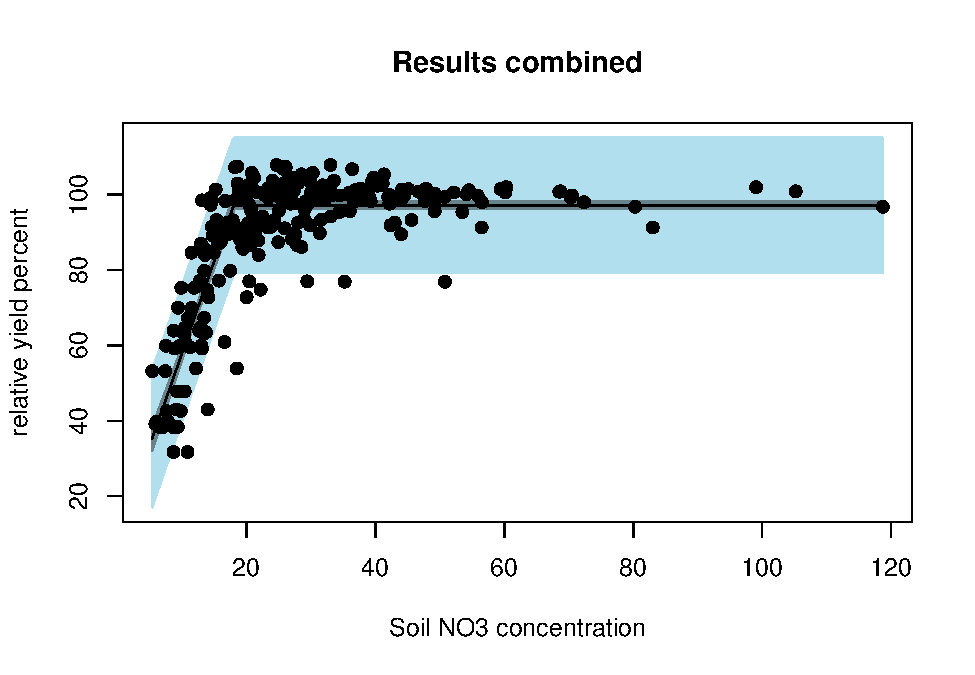
\includegraphics{06-nonlinear_regression_files/figure-latex/reduce-model-1.pdf}

Examine residual values for the combined model.

\begin{Shaded}
\begin{Highlighting}[]
\FunctionTok{library}\NormalTok{(nlstools)}
\CommentTok{\#using nlstools nlsResiduals function to get some quick residual plots}
\CommentTok{\#can also use test.nlsResiduals(resid)}
\CommentTok{\# https://www.rdocumentation.org/packages/nlstools/versions/1.0{-}2}
\NormalTok{resid }\OtherTok{\textless{}{-}} \FunctionTok{nlsResiduals}\NormalTok{(red\_nls)}
\FunctionTok{plot}\NormalTok{(resid)}
\end{Highlighting}
\end{Shaded}

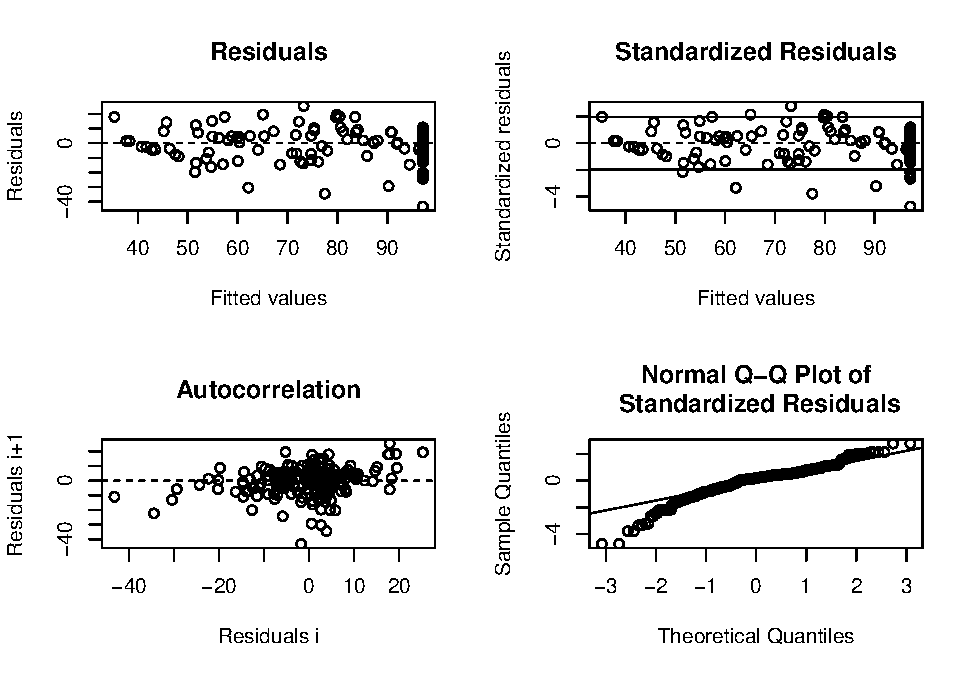
\includegraphics{06-nonlinear_regression_files/figure-latex/reduce-model-resid-1.pdf}

can we test whether the parameters for the two soil depth fits are significantly different? To know if the combined model is appropriate, we consider a parameterization where we let the parameters for the 60cm model be equal to the parameters from the 30cm model plus some increment:

\[
\beta_{02} = \beta_{01} + d_0 \\
\beta_{12} = \beta_{11} + d_1 \\
\alpha_{2} = \alpha_{1} + d_a
\]

We can implement this in the following function:

\begin{Shaded}
\begin{Highlighting}[]
\NormalTok{nonlinModelF }\OtherTok{\textless{}{-}} \ControlFlowTok{function}\NormalTok{(predictor,soildep,b01,b11,a1,d0,d1,da)\{}
\NormalTok{   b02 }\OtherTok{=}\NormalTok{ b01 }\SpecialCharTok{+}\NormalTok{ d0 }\CommentTok{\#make 60cm parms = 30cm parms + increment}
\NormalTok{   b12 }\OtherTok{=}\NormalTok{ b11 }\SpecialCharTok{+}\NormalTok{ d1}
\NormalTok{   a2 }\OtherTok{=}\NormalTok{ a1 }\SpecialCharTok{+}\NormalTok{ da}
   
\NormalTok{   y1 }\OtherTok{=} \FunctionTok{ifelse}\NormalTok{(predictor}\SpecialCharTok{\textless{}=}\NormalTok{a1, }
\NormalTok{         b01}\SpecialCharTok{+}\NormalTok{b11}\SpecialCharTok{*}\NormalTok{predictor, }\CommentTok{\#if observation less than cutoff simple linear model}
\NormalTok{         b01}\SpecialCharTok{+}\NormalTok{b11}\SpecialCharTok{*}\NormalTok{a1) }\CommentTok{\#otherwise flat line}
\NormalTok{   y2 }\OtherTok{=} \FunctionTok{ifelse}\NormalTok{(predictor}\SpecialCharTok{\textless{}=}\NormalTok{a2, }
\NormalTok{               b02}\SpecialCharTok{+}\NormalTok{b12}\SpecialCharTok{*}\NormalTok{predictor, }
\NormalTok{               b02}\SpecialCharTok{+}\NormalTok{b12}\SpecialCharTok{*}\NormalTok{a2) }
\NormalTok{   y }\OtherTok{=}\NormalTok{  y1}\SpecialCharTok{*}\NormalTok{(soildep }\SpecialCharTok{==} \DecValTok{30}\NormalTok{) }\SpecialCharTok{+}\NormalTok{ y2}\SpecialCharTok{*}\NormalTok{(soildep }\SpecialCharTok{==} \DecValTok{60}\NormalTok{)  }\CommentTok{\#combine models}
   \FunctionTok{return}\NormalTok{(y)}
\NormalTok{\}}
\end{Highlighting}
\end{Shaded}

Starting values are easy now because we fit each model individually.

\begin{Shaded}
\begin{Highlighting}[]
\NormalTok{Soil\_full}\OtherTok{=}\FunctionTok{nls}\NormalTok{(ryp}\SpecialCharTok{\textasciitilde{}}\FunctionTok{nonlinModelF}\NormalTok{(}\AttributeTok{predictor=}\NormalTok{no3,}\AttributeTok{soildep=}\NormalTok{depth,b01,b11,a1,d0,d1,da),}
              \AttributeTok{data=}\NormalTok{dat,}
              \AttributeTok{start=}\FunctionTok{list}\NormalTok{(}\AttributeTok{b01=}\FloatTok{15.2}\NormalTok{,}\AttributeTok{b11=}\FloatTok{3.58}\NormalTok{,}\AttributeTok{a1=}\FloatTok{23.13}\NormalTok{,}\AttributeTok{d0=}\SpecialCharTok{{-}}\FloatTok{9.74}\NormalTok{,}\AttributeTok{d1=}\FloatTok{2.11}\NormalTok{,}\AttributeTok{da=}\SpecialCharTok{{-}}\FloatTok{6.85}\NormalTok{)) }

\FunctionTok{summary}\NormalTok{(Soil\_full)}
\end{Highlighting}
\end{Shaded}

\begin{verbatim}
## 
## Formula: ryp ~ nonlinModelF(predictor = no3, soildep = depth, b01, b11, 
##     a1, d0, d1, da)
## 
## Parameters:
##     Estimate Std. Error t value Pr(>|t|)    
## b01  15.1943     2.8322   5.365 1.27e-07 ***
## b11   3.5760     0.1762  20.291  < 2e-16 ***
## a1   23.1324     0.4848  47.711  < 2e-16 ***
## d0   -9.7424     4.2357  -2.300   0.0219 *  
## d1    2.1060     0.3203   6.575 1.29e-10 ***
## da   -6.8461     0.5691 -12.030  < 2e-16 ***
## ---
## Signif. codes:  0 '***' 0.001 '**' 0.01 '*' 0.05 '.' 0.1 ' ' 1
## 
## Residual standard error: 7.854 on 474 degrees of freedom
## 
## Number of iterations to convergence: 1 
## Achieved convergence tolerance: 3.742e-06
\end{verbatim}

So, the increment parameters, \(d_1\),\(d_2\),\(d_a\) are all significantly different from 0, suggesting that we should have two models here.

\hypertarget{modelestiamtion-adequcy}{%
\subsection{Model/Estiamtion Adequcy}\label{modelestiamtion-adequcy}}

\citep{Bates_1980} assess nonlinearity in terms of 2 components of curvature:

\begin{itemize}
\item
  \textbf{Intrinsic nonlinearity}: the degree of bending and twisting in \(f(\theta)\); our estimation approach assumes that hte true function is relatively flat (planar) in the neighborhood fo \(\hat{\theta}\), which would not be true if \(f()\) has a lot of ``bending'' int he neighborhood of \(\hat{\theta}\) (independent of parameterizaiton)

  \begin{itemize}
  \item
    If bad, the distribution of residuals will be seriously distorted
  \item
    slow to converge
  \item
    difficult to identify ( could use this function \texttt{rms.curve})
  \item
    Solution:

    \begin{itemize}
    \tightlist
    \item
      could use higher order Taylor expansions estimation
    \item
      Bayesian method
    \end{itemize}
  \end{itemize}
\item
  \textbf{Parameter effects nonlinearity}: degree to which curvature (nonlinearity) is affected by choice of \(\theta\) (data dependent; dependent on parameterization)

  \begin{itemize}
  \tightlist
  \item
    leads to problems with inferecne on \(\hat{\theta}\)
  \item
    \texttt{rms.curve} in \texttt{MASS} can identify
  \item
    bootstrap-based inference can also be used
  \item
    Solution: try to reparaemterize.
  \end{itemize}
\end{itemize}

\begin{Shaded}
\begin{Highlighting}[]
\CommentTok{\#check parameter effects and intrinsic curvature}

\NormalTok{modD }\OtherTok{=} \FunctionTok{deriv3}\NormalTok{(}\SpecialCharTok{\textasciitilde{}}\NormalTok{ a}\SpecialCharTok{*}\FunctionTok{exp}\NormalTok{(b}\SpecialCharTok{*}\NormalTok{x), }\FunctionTok{c}\NormalTok{(}\StringTok{"a"}\NormalTok{,}\StringTok{"b"}\NormalTok{),}\ControlFlowTok{function}\NormalTok{(a,b,x) }\ConstantTok{NULL}\NormalTok{)}

\NormalTok{nlin\_modD}\OtherTok{=}\FunctionTok{nls}\NormalTok{(y}\SpecialCharTok{\textasciitilde{}}\FunctionTok{modD}\NormalTok{(a,b,x),}\AttributeTok{start=}\FunctionTok{list}\NormalTok{(}\AttributeTok{a=}\NormalTok{astrt,}\AttributeTok{b=}\NormalTok{bstrt),}\AttributeTok{data=}\NormalTok{datf)}

\FunctionTok{rms.curv}\NormalTok{(nlin\_modD)}
\end{Highlighting}
\end{Shaded}

\begin{verbatim}
## Parameter effects: c^theta x sqrt(F) = 0.0626 
##         Intrinsic: c^iota  x sqrt(F) = 0.0062
\end{verbatim}

In linear model, we have \protect\hyperlink{linear-regression}{Linear Regression}, we have goodness of fit measure as \(R^2\):

\[
R^2 = \frac{SSR}{SSTO} = 1- \frac{SSE}{SSTO} \\
= \frac{\sum_{i=1}^n (\hat{Y}_i- \bar{Y})^2}{\sum_{i=1}^n (Y_i- \bar{Y})^2} = 1- \frac{\sum_{i=1}^n ({Y}_i- \hat{Y})^2}{\sum_{i=1}^n (Y_i- \bar{Y})^2}
\]

but not valid in the nonlinear case because the error sum of squares and model sum of squares do not add to the total corrected sum of squares

\[
SSR + SSE \neq SST
\]

but we can use pseudo-\(R^2\):

\[
R^2_{pseudo} = 1 - \frac{\sum_{i=1}^n ({Y}_i- \hat{Y})^2}{\sum_{i=1}^n (Y_i- \bar{Y})^2}
\]

But we can't interpret this as the proportion of variability explained by the model. We should use as a relative comparison of different models.

\textbf{Residual Plots}: standardize, similar to OLS. useful when the intrinsic curvature is small:

The studentized residuals

\[
r_i = \frac{e_i}{s\sqrt{1-\hat{c}_i}}
\]

where \(\hat{c}_i\)is the i-th diagonal of \(\mathbf{\hat{H}= F(\hat{\theta})[F(\hat{\theta})'F(\hat{\theta})]^{-1}F(\hat{\theta})'}\)

We could have problems of

\begin{itemize}
\item
  Collinearity: the condition number of \(\mathbf{[F(\hat{\theta})'F(\hat{\theta})]^{-1}}\) should be less than 30. Follow \citep{Magel_1987}; reparameterize if possible
\item
  Leverage: Like \protect\hyperlink{ordinary-least-squares}{OLS}, but consider \(\mathbf{\hat{H}= F(\hat{\theta})[F(\hat{\theta})'F(\hat{\theta})]^{-1}F(\hat{\theta})'}\) (also known as ``tangent plant hat matrix'') \citep{Laurent_1992}
\item
  Heterogeneous Errors: weighted Non-linear Least Squares
\item
  Correlated Errors:

  \begin{itemize}
  \tightlist
  \item
    Generalized Nonlinear Least Squares
  \item
    Nonlinear Mixed Models
  \item
    Bayesian methods
  \end{itemize}
\end{itemize}

\hypertarget{application-2}{%
\subsection{Application}\label{application-2}}

\[
y_i = \frac{\theta_0 + \theta_1 x_i}{1 + \theta_2 \exp(0.4 x_i)} + \epsilon_i
\]

where \(i = 1,..,n\)

Get the starting values

\begin{verbatim}
## Warning: package 'dplyr' was built under R version 4.0.5
\end{verbatim}

\begin{verbatim}
## 
## Attaching package: 'dplyr'
\end{verbatim}

\begin{verbatim}
## The following object is masked from 'package:MASS':
## 
##     select
\end{verbatim}

\begin{verbatim}
## The following object is masked from 'package:kableExtra':
## 
##     group_rows
\end{verbatim}

\begin{verbatim}
## The following objects are masked from 'package:stats':
## 
##     filter, lag
\end{verbatim}

\begin{verbatim}
## The following objects are masked from 'package:base':
## 
##     intersect, setdiff, setequal, union
\end{verbatim}

\begin{Shaded}
\begin{Highlighting}[]
\FunctionTok{plot}\NormalTok{(my\_data)}
\end{Highlighting}
\end{Shaded}

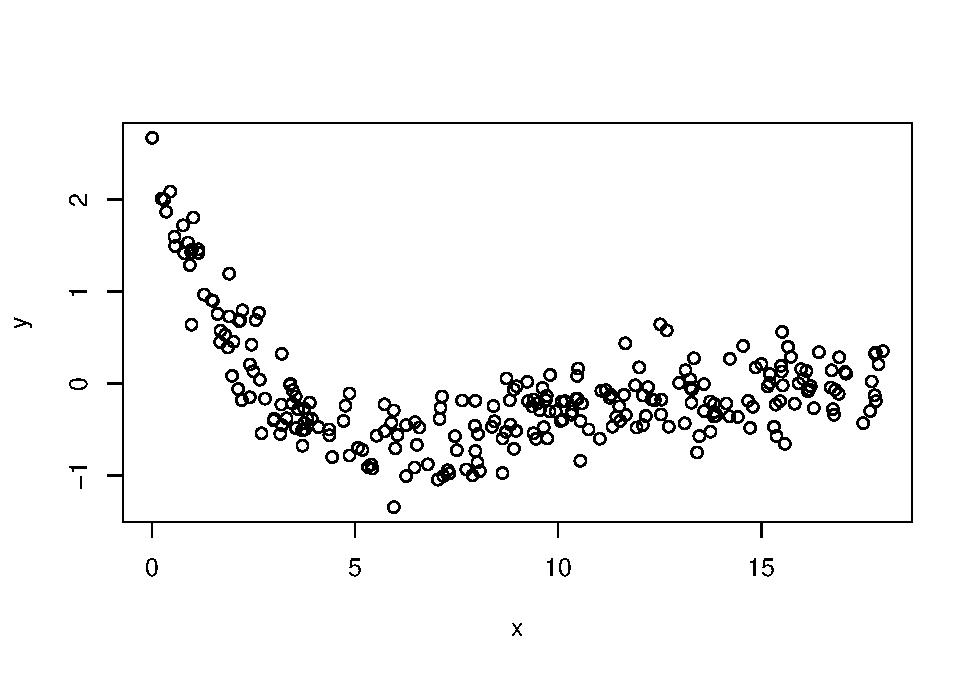
\includegraphics{06-nonlinear_regression_files/figure-latex/unnamed-chunk-18-1.pdf}

We notice that \(Y_{max} = \theta_0 + \theta_1 x_i\) in which we can find x\_i from data

\begin{Shaded}
\begin{Highlighting}[]
\FunctionTok{max}\NormalTok{(my\_data}\SpecialCharTok{$}\NormalTok{y)}
\end{Highlighting}
\end{Shaded}

\begin{verbatim}
## [1] 2.6722
\end{verbatim}

\begin{Shaded}
\begin{Highlighting}[]
\NormalTok{my\_data}\SpecialCharTok{$}\NormalTok{x[}\FunctionTok{which.max}\NormalTok{(my\_data}\SpecialCharTok{$}\NormalTok{y)]}
\end{Highlighting}
\end{Shaded}

\begin{verbatim}
## [1] 0.0094
\end{verbatim}

hence, x = 0.0094 when y = 2.6722 when we have the first equation as

\[
2.6722 = \theta_0 + 0.0094 \theta_1 \\
\theta_0 + 0.0094 \theta_1 + 0 \theta_2 = 2.6722
\]

Secondly, we notice that we can obtain the ``average'' of y when

\[
1+ \theta_2 exp(0.4 x) = 2
\]

then we can find this average numbers of x and y

\begin{Shaded}
\begin{Highlighting}[]
\FunctionTok{mean}\NormalTok{(my\_data}\SpecialCharTok{$}\NormalTok{y) }\CommentTok{\#find mean y}
\end{Highlighting}
\end{Shaded}

\begin{verbatim}
## [1] -0.0747864
\end{verbatim}

\begin{Shaded}
\begin{Highlighting}[]
\NormalTok{my\_data}\SpecialCharTok{$}\NormalTok{y[}\FunctionTok{which.min}\NormalTok{(}\FunctionTok{abs}\NormalTok{(my\_data}\SpecialCharTok{$}\NormalTok{y}\SpecialCharTok{{-}}\NormalTok{(}\FunctionTok{mean}\NormalTok{(my\_data}\SpecialCharTok{$}\NormalTok{y))))] }\CommentTok{\# find y closest to its mean}
\end{Highlighting}
\end{Shaded}

\begin{verbatim}
## [1] -0.0773
\end{verbatim}

\begin{Shaded}
\begin{Highlighting}[]
\NormalTok{my\_data}\SpecialCharTok{$}\NormalTok{x[}\FunctionTok{which.min}\NormalTok{(}\FunctionTok{abs}\NormalTok{(my\_data}\SpecialCharTok{$}\NormalTok{y}\SpecialCharTok{{-}}\NormalTok{(}\FunctionTok{mean}\NormalTok{(my\_data}\SpecialCharTok{$}\NormalTok{y))))] }\CommentTok{\#find x closest to the mean y}
\end{Highlighting}
\end{Shaded}

\begin{verbatim}
## [1] 11.0648
\end{verbatim}

we have the second equation

\[
1 + \theta_2 exp(0.4*11.0648) = 2 \\
0 \theta_1 + 0 \theta_1 + 83.58967 \theta_2 = 1
\]

Thirdly, we can plug in the value of x closest to 1 to find the value of y

\begin{Shaded}
\begin{Highlighting}[]
\NormalTok{my\_data}\SpecialCharTok{$}\NormalTok{x[}\FunctionTok{which.min}\NormalTok{(}\FunctionTok{abs}\NormalTok{(my\_data}\SpecialCharTok{$}\NormalTok{x}\DecValTok{{-}1}\NormalTok{))] }\CommentTok{\# find value of x closet to 1}
\end{Highlighting}
\end{Shaded}

\begin{verbatim}
## [1] 0.9895
\end{verbatim}

\begin{Shaded}
\begin{Highlighting}[]
\FunctionTok{match}\NormalTok{(my\_data}\SpecialCharTok{$}\NormalTok{x[}\FunctionTok{which.min}\NormalTok{(}\FunctionTok{abs}\NormalTok{(my\_data}\SpecialCharTok{$}\NormalTok{x}\DecValTok{{-}1}\NormalTok{))], my\_data}\SpecialCharTok{$}\NormalTok{x) }\CommentTok{\# find index of x closest to 1}
\end{Highlighting}
\end{Shaded}

\begin{verbatim}
## [1] 14
\end{verbatim}

\begin{Shaded}
\begin{Highlighting}[]
\NormalTok{my\_data}\SpecialCharTok{$}\NormalTok{y[}\FunctionTok{match}\NormalTok{(my\_data}\SpecialCharTok{$}\NormalTok{x[}\FunctionTok{which.min}\NormalTok{(}\FunctionTok{abs}\NormalTok{(my\_data}\SpecialCharTok{$}\NormalTok{x}\DecValTok{{-}1}\NormalTok{))], my\_data}\SpecialCharTok{$}\NormalTok{x)]}\CommentTok{\# find y value}
\end{Highlighting}
\end{Shaded}

\begin{verbatim}
## [1] 1.4577
\end{verbatim}

hence we have

\[
1.457 = \frac{\theta_0 + \theta_1*0.9895}{1 + \theta_2 exp(0.4*0.9895)} \\
1.457 + 2.164479 *\theta_2 = \theta_0 + \theta_1*0.9895 \\
\theta_0 + \theta_1*0.9895 -  2.164479 *\theta_2 = 1.457
\]

with 3 equations, we can solve them to get the starting value for \(\theta_0,\theta_1, \theta_2\)

\[
\theta_0 + 0.0094 \theta_1 + 0 \theta_2 = 2.6722 \\
0 \theta_1 + 0 \theta_1 + 83.58967 \theta_2 = 1 \\
\theta_0 + \theta_1*0.9895 -  2.164479 *\theta_2 = 1.457
\]

\begin{Shaded}
\begin{Highlighting}[]
\FunctionTok{library}\NormalTok{(matlib) }
\NormalTok{A }\OtherTok{=} \FunctionTok{matrix}\NormalTok{(}\FunctionTok{c}\NormalTok{(}\DecValTok{0}\NormalTok{,}\FloatTok{0.0094}\NormalTok{, }\DecValTok{0}\NormalTok{, }\DecValTok{0}\NormalTok{,}\DecValTok{0}\NormalTok{, }\FloatTok{83.58967}\NormalTok{, }\DecValTok{1}\NormalTok{, }\FloatTok{0.9895}\NormalTok{, }\SpecialCharTok{{-}} \FloatTok{2.164479}\NormalTok{), }\AttributeTok{nrow =} \DecValTok{3}\NormalTok{, }\AttributeTok{ncol =} \DecValTok{3}\NormalTok{, }\AttributeTok{byrow =}\NormalTok{ T)}
\NormalTok{b }\OtherTok{=} \FunctionTok{c}\NormalTok{(}\FloatTok{2.6722}\NormalTok{,}\DecValTok{1}\NormalTok{,}\FloatTok{1.457}\NormalTok{ )}
\FunctionTok{showEqn}\NormalTok{(A, b)}
\end{Highlighting}
\end{Shaded}

\begin{verbatim}
## 0*x1 + 0.0094*x2        + 0*x3  =  2.6722 
## 0*x1      + 0*x2 + 83.58967*x3  =       1 
## 1*x1 + 0.9895*x2 - 2.164479*x3  =   1.457
\end{verbatim}

\begin{Shaded}
\begin{Highlighting}[]
\FunctionTok{Solve}\NormalTok{(A, b, }\AttributeTok{fractions =}\NormalTok{ F)}
\end{Highlighting}
\end{Shaded}

\begin{verbatim}
## x1      =  -279.80879739 
##   x2    =   284.27659574 
##     x3  =      0.0119632
\end{verbatim}

Construct manually \protect\hyperlink{gauss-newton-algorithm}{Gauss-Newton Algorithm}

\begin{Shaded}
\begin{Highlighting}[]
\CommentTok{\#starting value}
\NormalTok{theta\_0\_strt }\OtherTok{=} \SpecialCharTok{{-}}\FloatTok{279.80879739} 
\NormalTok{theta\_1\_strt }\OtherTok{=}  \FloatTok{284.27659574} 
\NormalTok{theta\_2\_strt }\OtherTok{=} \FloatTok{0.0119632} 

\CommentTok{\#model}
\NormalTok{mod\_4 }\OtherTok{=} \ControlFlowTok{function}\NormalTok{(theta\_0,theta\_1,theta\_2,x)\{}
\NormalTok{    (theta\_0 }\SpecialCharTok{+}\NormalTok{ theta\_1}\SpecialCharTok{*}\NormalTok{x)}\SpecialCharTok{/}\NormalTok{(}\DecValTok{1}\SpecialCharTok{+}\NormalTok{ theta\_2}\SpecialCharTok{*}\FunctionTok{exp}\NormalTok{(}\FloatTok{0.4}\SpecialCharTok{*}\NormalTok{x))}
\NormalTok{\}}

\CommentTok{\#define a function}
\NormalTok{f\_4 }\OtherTok{=} \FunctionTok{expression}\NormalTok{((theta\_0 }\SpecialCharTok{+}\NormalTok{ theta\_1}\SpecialCharTok{*}\NormalTok{x)}\SpecialCharTok{/}\NormalTok{(}\DecValTok{1}\SpecialCharTok{+}\NormalTok{ theta\_2}\SpecialCharTok{*}\FunctionTok{exp}\NormalTok{(}\FloatTok{0.4}\SpecialCharTok{*}\NormalTok{x)))}

\CommentTok{\#take the first derivative}
\NormalTok{df\_4.d\_theta\_0}\OtherTok{=}\FunctionTok{D}\NormalTok{(f\_4,}\StringTok{\textquotesingle{}theta\_0\textquotesingle{}}\NormalTok{)}

\NormalTok{df\_4.d\_theta\_1}\OtherTok{=}\FunctionTok{D}\NormalTok{(f\_4,}\StringTok{\textquotesingle{}theta\_1\textquotesingle{}}\NormalTok{)}

\NormalTok{df\_4.d\_theta\_2}\OtherTok{=}\FunctionTok{D}\NormalTok{(f\_4,}\StringTok{\textquotesingle{}theta\_2\textquotesingle{}}\NormalTok{)}

\CommentTok{\# save the result of all iterations}
\NormalTok{theta\_vec }\OtherTok{=} \FunctionTok{matrix}\NormalTok{(}\FunctionTok{c}\NormalTok{(theta\_0\_strt,theta\_1\_strt,theta\_2\_strt))}
\NormalTok{delta}\OtherTok{=} \FunctionTok{matrix}\NormalTok{(}\ConstantTok{NA}\NormalTok{, }\AttributeTok{nrow=}\DecValTok{3}\NormalTok{,}\AttributeTok{ncol =} \DecValTok{1}\NormalTok{)}

\NormalTok{f\_theta }\OtherTok{=} \FunctionTok{as.matrix}\NormalTok{(}\FunctionTok{eval}\NormalTok{(f\_4,}\FunctionTok{list}\NormalTok{(}\AttributeTok{x=}\NormalTok{my\_data}\SpecialCharTok{$}\NormalTok{x,}\AttributeTok{theta\_0 =}\NormalTok{ theta\_vec[}\DecValTok{1}\NormalTok{,}\DecValTok{1}\NormalTok{],}\AttributeTok{theta\_1 =}\NormalTok{ theta\_vec[}\DecValTok{2}\NormalTok{,}\DecValTok{1}\NormalTok{],}\AttributeTok{theta\_2 =}\NormalTok{ theta\_vec[}\DecValTok{3}\NormalTok{,}\DecValTok{1}\NormalTok{])))}

\NormalTok{i }\OtherTok{=} \DecValTok{1}

\ControlFlowTok{repeat}\NormalTok{ \{}
\NormalTok{    F\_theta\_0 }\OtherTok{=} \FunctionTok{as.matrix}\NormalTok{(}\FunctionTok{cbind}\NormalTok{(}
        \FunctionTok{eval}\NormalTok{(}
\NormalTok{            df\_4.d\_theta\_0,}
            \FunctionTok{list}\NormalTok{(}
                \AttributeTok{x =}\NormalTok{ my\_data}\SpecialCharTok{$}\NormalTok{x,}
                \AttributeTok{theta\_0 =}\NormalTok{ theta\_vec[}\DecValTok{1}\NormalTok{, i],}
                \AttributeTok{theta\_1 =}\NormalTok{ theta\_vec[}\DecValTok{2}\NormalTok{, i],}
                \AttributeTok{theta\_2 =}\NormalTok{ theta\_vec[}\DecValTok{3}\NormalTok{, i]}
\NormalTok{            )}
\NormalTok{        ),}
        \FunctionTok{eval}\NormalTok{(}
\NormalTok{            df\_4.d\_theta\_1,}
            \FunctionTok{list}\NormalTok{(}
                \AttributeTok{x =}\NormalTok{ my\_data}\SpecialCharTok{$}\NormalTok{x,}
                \AttributeTok{theta\_0 =}\NormalTok{ theta\_vec[}\DecValTok{1}\NormalTok{, i],}
                \AttributeTok{theta\_1 =}\NormalTok{ theta\_vec[}\DecValTok{2}\NormalTok{, i],}
                \AttributeTok{theta\_2 =}\NormalTok{ theta\_vec[}\DecValTok{3}\NormalTok{, i]}
\NormalTok{            )}
\NormalTok{        ),}
        \FunctionTok{eval}\NormalTok{(}
\NormalTok{            df\_4.d\_theta\_2,}
            \FunctionTok{list}\NormalTok{(}
                \AttributeTok{x =}\NormalTok{ my\_data}\SpecialCharTok{$}\NormalTok{x,}
                \AttributeTok{theta\_0 =}\NormalTok{ theta\_vec[}\DecValTok{1}\NormalTok{, i],}
                \AttributeTok{theta\_1 =}\NormalTok{ theta\_vec[}\DecValTok{2}\NormalTok{, i],}
                \AttributeTok{theta\_2 =}\NormalTok{ theta\_vec[}\DecValTok{3}\NormalTok{, i]}
\NormalTok{            )}
\NormalTok{        )}
\NormalTok{    ))}
\NormalTok{    delta[, i] }\OtherTok{=}\NormalTok{ (}\FunctionTok{solve}\NormalTok{(}\FunctionTok{t}\NormalTok{(F\_theta\_0) }\SpecialCharTok{\%*\%}\NormalTok{ F\_theta\_0)) }\SpecialCharTok{\%*\%} \FunctionTok{t}\NormalTok{(F\_theta\_0) }\SpecialCharTok{\%*\%}\NormalTok{ (my\_data}\SpecialCharTok{$}\NormalTok{y }\SpecialCharTok{{-}}\NormalTok{ f\_theta[,i])}
\NormalTok{    theta\_vec }\OtherTok{=} \FunctionTok{cbind}\NormalTok{(theta\_vec, }\FunctionTok{matrix}\NormalTok{(}\ConstantTok{NA}\NormalTok{, }\AttributeTok{nrow =} \DecValTok{3}\NormalTok{, }\AttributeTok{ncol =} \DecValTok{1}\NormalTok{))}
\NormalTok{    theta\_vec[, i}\SpecialCharTok{+}\DecValTok{1}\NormalTok{] }\OtherTok{=}\NormalTok{ theta\_vec[, i] }\SpecialCharTok{+}\NormalTok{ delta[, i]}
\NormalTok{    i }\OtherTok{=}\NormalTok{ i }\SpecialCharTok{+} \DecValTok{1}
    
\NormalTok{    f\_theta }\OtherTok{=} \FunctionTok{cbind}\NormalTok{(f\_theta, }\FunctionTok{as.matrix}\NormalTok{(}\FunctionTok{eval}\NormalTok{(}
\NormalTok{        f\_4,}
        \FunctionTok{list}\NormalTok{(}
            \AttributeTok{x =}\NormalTok{ my\_data}\SpecialCharTok{$}\NormalTok{x,}
            \AttributeTok{theta\_0 =}\NormalTok{ theta\_vec[}\DecValTok{1}\NormalTok{, i],}
            \AttributeTok{theta\_1 =}\NormalTok{ theta\_vec[}\DecValTok{2}\NormalTok{, i],}
            \AttributeTok{theta\_2 =}\NormalTok{ theta\_vec[}\DecValTok{3}\NormalTok{, i]}
\NormalTok{        )}
\NormalTok{    )))}
\NormalTok{    delta }\OtherTok{=} \FunctionTok{cbind}\NormalTok{(delta, }\FunctionTok{matrix}\NormalTok{(}\ConstantTok{NA}\NormalTok{, }\AttributeTok{nrow =} \DecValTok{3}\NormalTok{, }\AttributeTok{ncol =} \DecValTok{1}\NormalTok{))}
    
    \CommentTok{\#convergence criteria based on SSE}
    \ControlFlowTok{if}\NormalTok{ (}\FunctionTok{abs}\NormalTok{(}\FunctionTok{sum}\NormalTok{((my\_data}\SpecialCharTok{$}\NormalTok{y }\SpecialCharTok{{-}}\NormalTok{ f\_theta[,i])}\SpecialCharTok{\^{}}\DecValTok{2}\NormalTok{)}\SpecialCharTok{{-}}\FunctionTok{sum}\NormalTok{((my\_data}\SpecialCharTok{$}\NormalTok{y }\SpecialCharTok{{-}}\NormalTok{ f\_theta[,i}\DecValTok{{-}1}\NormalTok{])}\SpecialCharTok{\^{}}\DecValTok{2}\NormalTok{))}\SpecialCharTok{/}\NormalTok{(}\FunctionTok{sum}\NormalTok{((my\_data}\SpecialCharTok{$}\NormalTok{y }\SpecialCharTok{{-}}\NormalTok{ f\_theta[,i}\DecValTok{{-}1}\NormalTok{])}\SpecialCharTok{\^{}}\DecValTok{2}\NormalTok{))}\SpecialCharTok{\textless{}}\FloatTok{0.001}\NormalTok{)\{}
        \ControlFlowTok{break}
\NormalTok{    \}}
\NormalTok{\}}
\NormalTok{delta}
\end{Highlighting}
\end{Shaded}

\begin{verbatim}
##               [,1]        [,2]        [,3]       [,4]       [,5]       [,6]
## [1,]  2.811840e+02 -0.03929013  0.43160654  0.6904856  0.6746748  0.4056460
## [2,] -2.846545e+02  0.03198446 -0.16403964 -0.2895487 -0.2933345 -0.1734087
## [3,] -1.804567e-05  0.01530258  0.05137285  0.1183271  0.1613129  0.1160404
##             [,7] [,8]
## [1,]  0.09517681   NA
## [2,] -0.03928239   NA
## [3,]  0.03004911   NA
\end{verbatim}

\begin{Shaded}
\begin{Highlighting}[]
\NormalTok{theta\_vec}
\end{Highlighting}
\end{Shaded}

\begin{verbatim}
##              [,1]        [,2]        [,3]        [,4]       [,5]       [,6]
## [1,] -279.8087974  1.37521388  1.33592375  1.76753029  2.4580158  3.1326907
## [2,]  284.2765957 -0.37788712 -0.34590266 -0.50994230 -0.7994910 -1.0928255
## [3,]    0.0119632  0.01194515  0.02724773  0.07862059  0.1969477  0.3582607
##            [,7]       [,8]
## [1,]  3.5383367  3.6335135
## [2,] -1.2662342 -1.3055166
## [3,]  0.4743011  0.5043502
\end{verbatim}

\begin{Shaded}
\begin{Highlighting}[]
\FunctionTok{head}\NormalTok{(f\_theta)}
\end{Highlighting}
\end{Shaded}

\begin{verbatim}
##           [,1]     [,2]     [,3]     [,4]     [,5]     [,6]     [,7]     [,8]
## [1,] -273.8482 1.355410 1.297194 1.633802 2.046023 2.296554 2.389041 2.404144
## [2,] -209.0859 1.268192 1.216738 1.514575 1.863098 2.059505 2.126009 2.135969
## [3,] -190.3323 1.242916 1.193433 1.480136 1.810629 1.992095 2.051603 2.060202
## [4,] -177.1891 1.225196 1.177099 1.456024 1.774000 1.945197 1.999945 2.007625
## [5,] -148.5872 1.186618 1.141549 1.403631 1.694715 1.844154 1.888953 1.894730
## [6,] -119.9585 1.147980 1.105961 1.351301 1.615968 1.744450 1.779859 1.783866
\end{verbatim}

\begin{Shaded}
\begin{Highlighting}[]
\CommentTok{\# estimate sigma\^{}2 }

\NormalTok{sigma2 }\OtherTok{=} \DecValTok{1} \SpecialCharTok{/}\NormalTok{ (}\FunctionTok{nrow}\NormalTok{(my\_data) }\SpecialCharTok{{-}} \DecValTok{3}\NormalTok{) }\SpecialCharTok{*}\NormalTok{ (}\FunctionTok{t}\NormalTok{(my\_data}\SpecialCharTok{$}\NormalTok{y }\SpecialCharTok{{-}}\NormalTok{ (f\_theta[, }\FunctionTok{ncol}\NormalTok{(f\_theta)]))) }\SpecialCharTok{\%*\%}
\NormalTok{    (my\_data}\SpecialCharTok{$}\NormalTok{y }\SpecialCharTok{{-}}\NormalTok{ (f\_theta[, }\FunctionTok{ncol}\NormalTok{(f\_theta)])) }\CommentTok{\# p = 3}
\NormalTok{sigma2}
\end{Highlighting}
\end{Shaded}

\begin{verbatim}
##           [,1]
## [1,] 0.0801686
\end{verbatim}

After 8 iterations, my function has converged. And objective function value at convergence is

\begin{Shaded}
\begin{Highlighting}[]
\FunctionTok{sum}\NormalTok{((my\_data}\SpecialCharTok{$}\NormalTok{y }\SpecialCharTok{{-}}\NormalTok{ f\_theta[,i])}\SpecialCharTok{\^{}}\DecValTok{2}\NormalTok{)}
\end{Highlighting}
\end{Shaded}

\begin{verbatim}
## [1] 19.80165
\end{verbatim}

and the parameters of \(\theta\)s are

\begin{Shaded}
\begin{Highlighting}[]
\NormalTok{theta\_vec[,}\FunctionTok{ncol}\NormalTok{(theta\_vec)]}
\end{Highlighting}
\end{Shaded}

\begin{verbatim}
## [1]  3.6335135 -1.3055166  0.5043502
\end{verbatim}

and the asymptotic variance covariance matrix is

\begin{Shaded}
\begin{Highlighting}[]
\FunctionTok{as.numeric}\NormalTok{(sigma2)}\SpecialCharTok{*}\FunctionTok{as.matrix}\NormalTok{(}\FunctionTok{solve}\NormalTok{(}\FunctionTok{crossprod}\NormalTok{(F\_theta\_0)))}
\end{Highlighting}
\end{Shaded}

\begin{verbatim}
##             [,1]        [,2]        [,3]
## [1,]  0.11552571 -0.04817428  0.02685848
## [2,] -0.04817428  0.02100861 -0.01158212
## [3,]  0.02685848 -0.01158212  0.00703916
\end{verbatim}

Issue that I encounter in this problem was that it was very sensitive to starting values. when I tried the value of 1 for all \(\theta\)s, I have vastly different parameter estimates. Then, I try to use the model interpretation to try to find reasonable starting values.

Check with predefined function in nls

\begin{Shaded}
\begin{Highlighting}[]
\NormalTok{nlin\_4 }\OtherTok{=} \FunctionTok{nls}\NormalTok{(y }\SpecialCharTok{\textasciitilde{}} \FunctionTok{mod\_4}\NormalTok{(theta\_0,theta\_1, theta\_2, x), }\AttributeTok{start =} \FunctionTok{list}\NormalTok{(}\AttributeTok{theta\_0=}\SpecialCharTok{{-}}\FloatTok{279.80879739}\NormalTok{ ,}\AttributeTok{theta\_1=}\FloatTok{284.27659574}\NormalTok{ , }\AttributeTok{theta\_2=}\FloatTok{0.0119632}\NormalTok{), }\AttributeTok{data =}\NormalTok{ my\_data)}
\NormalTok{nlin\_4}
\end{Highlighting}
\end{Shaded}

\begin{verbatim}
## Nonlinear regression model
##   model: y ~ mod_4(theta_0, theta_1, theta_2, x)
##    data: my_data
## theta_0 theta_1 theta_2 
##  3.6359 -1.3064  0.5053 
##  residual sum-of-squares: 19.8
## 
## Number of iterations to convergence: 9 
## Achieved convergence tolerance: 2.294e-07
\end{verbatim}

\hypertarget{generalized-linear-models}{%
\chapter{Generalized Linear Models}\label{generalized-linear-models}}

Even though we call it generalized linear model, it is still under the paradigm of non-linear regression, because the form of the regression model is non-linear. The name generalized linear model derived from the fact that we have \(\mathbf{x'_i \beta}\) (which is linear form) in the model.

\hypertarget{logistic-regression}{%
\section{Logistic Regression}\label{logistic-regression}}

\[
p_i = f(\mathbf{x}_i ; \beta) = \frac{exp(\mathbf{x_i'\beta})}{1 + exp(\mathbf{x_i'\beta})}
\]

Equivalently,

\[
logit(p_i) = log(\frac{p_i}{1+p_i}) = \mathbf{x_i'\beta}
\]

where \(\frac{p_i}{1+p_i}\)is the \textbf{odds}.

In this form, the model is specified such that \textbf{a function of the mean response is linear}. Hence, \textbf{Generalized Linear Models}

The likelihood function

\[
L(p_i) = \prod_{i=1}^{n} p_i^{Y_i}(1-p_i)^{1-Y_i}
\]

where \(p_i = \frac{\mathbf{x'_i \beta}}{1+\mathbf{x'_i \beta}}\) and \(1-p_i = (1+ exp(\mathbf{x'_i \beta}))^{-1}\)

Hence, our objective function is

\[
Q(\beta) = log(L(\beta)) = \sum_{i=1}^n Y_i \mathbf{x'_i \beta} - \sum_{i=1}^n  log(1+ exp(\mathbf{x'_i \beta}))
\]

we could maximize this function numerically using the optimization method above, which allows us to find numerical MLE for \(\hat{\beta}\). Then we can use the standard asymptotic properties of MLEs to make inference.

Property of MLEs is that parameters are asymptotically unbiased with sample variance-covariance matrix given by the \textbf{inverse Fisher information matrix}

\[
\hat{\beta} \dot{\sim} AN(\beta,[\mathbf{I}(\beta)]^{-1})
\]

where the \textbf{Fisher Information matrix}, \(\mathbf{I}(\beta)\) is

\[
\begin{aligned}
\mathbf{I}(\beta) &= E[\frac{\partial \log(L(\beta))}{\partial (\beta)}\frac{\partial \log(L(\beta))}{\partial \beta'}] \\
&= E[(\frac{\partial \log(L(\beta))}{\partial \beta_i} \frac{\partial \log(L(\beta))}{\partial \beta_j})_{ij}]
\end{aligned}
\]

Under \textbf{regularity conditions}, this is equivalent to the negative of the expected value of the Hessian Matrix

\[
\begin{aligned}
\mathbf{I}(\beta) &= -E[\frac{\partial^2 \log(L(\beta))}{\partial \beta \partial \beta'}] \\
&= -E[(\frac{\partial^2 \log(L(\beta))}{\partial \beta_i \partial \beta_j})_{ij}]
\end{aligned}
\]

Example:

\[
x_i' \beta = \beta_0 + \beta_1 x_i
\]

\[
- \frac{\partial^2 \ln(L(\beta))}{\partial \beta^2_0} = \sum_{i=1}^n \frac{\exp(x'_i \beta)}{1 + \exp(x'_i \beta)} - [\frac{\exp(x_i' \beta)}{1+ \exp(x'_i \beta)}]^2 = \sum_{i=1}^n p_i (1-p_i) \\
- \frac{\partial^2 \ln(L(\beta))}{\partial \beta^2_1} = \sum_{i=1}^n \frac{x_i^2\exp(x'_i \beta)}{1 + \exp(x'_i \beta)} - [\frac{x_i\exp(x_i' \beta)}{1+ \exp(x'_i \beta)}]^2 = \sum_{i=1}^n x_i^2p_i (1-p_i) \\
- \frac{\partial^2 \ln(L(\beta))}{\partial \beta_0 \partial \beta_1} = \sum_{i=1}^n \frac{x_i\exp(x'_i \beta)}{1 + \exp(x'_i \beta)} - x_i[\frac{\exp(x_i' \beta)}{1+ \exp(x'_i \beta)}]^2 = \sum_{i=1}^n x_ip_i (1-p_i) \\
\]

Hence,

\[
\mathbf{I} (\beta) = 
\left[
\begin{array}
{cc}
\sum_i p_i(1-p_i) & \sum_i x_i p_i(1-p_i) \\
\sum_i x_i p_i(1-p_i) & \sum_i x_i^2 p_i(1-p_i)
\end{array}
\right]
\]

\textbf{Inference}

\textbf{Likelihood Ratio Tests}

To formulate the test, let \(\beta = [\beta_1', \beta_2']'\). If you are interested in testing a hypothesis about \(\beta_1\), then we leave \(\beta_2\) unspecified (called \textbf{nuisance parameters}). \(\beta_1\) and \(\beta_2\) can either a \textbf{vector} or \textbf{scalar}, or \(\beta_2\) can be null.

Example: \(H_0: \beta_1 = \beta_{1,0}\) (where \(\beta_{1,0}\) is specified) and \(\hat{\beta}_{2,0}\) be the MLE of \(\beta_2\) under the restriction that \(\beta_1 = \beta_{1,0}\). The likelihood ratio test statistic is

\[
-2\log\Lambda = -2[\log(L(\beta_{1,0},\hat{\beta}_{2,0})) - \log(L(\hat{\beta}_1,\hat{\beta}_2))]
\]

where

\begin{itemize}
\tightlist
\item
  the first term is the value fo the likelihood for the fitted restricted model\\
\item
  the second term is the likelihood value of the fitted unrestricted model
\end{itemize}

Under the null,

\[
-2 \log \Lambda \sim \chi^2_{\upsilon}
\]

where \(\upsilon\) is the dimension of \(\beta_1\)

We reject the null when \(-2\log \Lambda > \chi_{\upsilon,1-\alpha}^2\)

\textbf{Wald Statistics}

Based on

\[
\hat{\beta} \sim AN (\beta, [\mathbf{I}(\beta)^{-1}])
\]

\[
H_0: \mathbf{L}\hat{\beta} = 0 
\]

where \(\mathbf{L}\) is a q x p matrix with q linearly independent rows. Then

\[
W = (\mathbf{L\hat{\beta}})'(\mathbf{L[I(\hat{\beta})]^{-1}L'})^{-1}(\mathbf{L\hat{\beta}})
\]

under the null hypothesis

Confidence interval

\[
\hat{\beta}_i \pm 1.96 \hat{s}_{ii}^2
\]

where \(\hat{s}_{ii}^2\) is the i-th diagonal of \(\mathbf{[I(\hat{\beta})]}^{-1}\)

If you have

\begin{itemize}
\tightlist
\item
  large sample size, the likelihood ratio and Wald tests have similar results.\\
\item
  small sample size, the likelihood ratio test is better.
\end{itemize}

\textbf{Logistic Regression: Interpretation of} \(\beta\)

For single regressor, the model is

\[
logit\{\hat{p}_{x_i}\} \equiv logit (\hat{p}_i) = \log(\frac{\hat{p}_i}{1 - \hat{p}_i}) = \hat{\beta}_0 + \hat{\beta}_1 x_i
\]

When \(x= x_i + 1\)

\[
logit\{\hat{p}_{x_i +1}\} = \hat{\beta}_0 + \hat{\beta}(x_i + 1) = logit\{\hat{p}_{x_i}\} + \hat{\beta}_1
\]

Then,

\[
logit\{\hat{p}_{x_i +1}\} - logit\{\hat{p}_{x_i}\} = log\{odds[\hat{p}_{x_i +1}]\} - log\{odds[\hat{p}_{x_i}]\} \\
= log(\frac{odds[\hat{p}_{x_i + 1}]}{odds[\hat{p}_{x_i}]}) = \hat{\beta}_1
\]

and

\[
exp(\hat{\beta}_1) = \frac{odds[\hat{p}_{x_i + 1}]}{odds[\hat{p}_{x_i}]}
\]

the estimated \textbf{odds ratio}

the estimated odds ratio, when there is a difference of c units in the regressor x, is \(exp(c\hat{\beta}_1)\). When there are multiple covariates, \(exp(\hat{\beta}_k)\) is the estimated odds ratio for the variable \(x_k\), assuming that all of the other variables are held constant.

\textbf{Inference on the Mean Response}

Let \(x_h = (1, x_{h1}, ...,x_{h,p-1})'\). Then

\[
\hat{p}_h = \frac{exp(\mathbf{x'_h \hat{\beta}})}{1 + exp(\mathbf{x'_h \hat{\beta}})}
\]

and \(s^2(\hat{p}_h) = \mathbf{x'_h[I(\hat{\beta})]^{-1}x_h}\)

For new observation, we can have a cutoff point to decide whether y = 0 or 1.

\hypertarget{application-3}{%
\subsection{Application}\label{application-3}}

\begin{Shaded}
\begin{Highlighting}[]
\FunctionTok{library}\NormalTok{(kableExtra)}
\FunctionTok{library}\NormalTok{(dplyr)}
\FunctionTok{library}\NormalTok{(pscl)}
\end{Highlighting}
\end{Shaded}

\begin{verbatim}
## Classes and Methods for R developed in the
## Political Science Computational Laboratory
## Department of Political Science
## Stanford University
## Simon Jackman
## hurdle and zeroinfl functions by Achim Zeileis
\end{verbatim}

\begin{Shaded}
\begin{Highlighting}[]
\FunctionTok{library}\NormalTok{(ggplot2)}
\FunctionTok{library}\NormalTok{(faraway)}
\end{Highlighting}
\end{Shaded}

\begin{verbatim}
## 
## Attaching package: 'faraway'
\end{verbatim}

\begin{verbatim}
## The following object is masked from 'package:investr':
## 
##     beetle
\end{verbatim}

\begin{Shaded}
\begin{Highlighting}[]
\FunctionTok{library}\NormalTok{(nnet)}
\end{Highlighting}
\end{Shaded}

\begin{verbatim}
## Warning: package 'nnet' was built under R version 4.0.5
\end{verbatim}

\begin{Shaded}
\begin{Highlighting}[]
\FunctionTok{library}\NormalTok{(agridat)}
\FunctionTok{library}\NormalTok{(nlstools)}
\end{Highlighting}
\end{Shaded}

Logistic Regression

\(x \sim Unif(-0.5,2.5)\). Then \(\eta = 0.5 + 0.75 x\)

\begin{Shaded}
\begin{Highlighting}[]
\FunctionTok{set.seed}\NormalTok{(}\DecValTok{23}\NormalTok{) }\CommentTok{\#set seed for reproducibility}
\NormalTok{x }\OtherTok{\textless{}{-}} \FunctionTok{runif}\NormalTok{(}\DecValTok{1000}\NormalTok{,}\AttributeTok{min =} \SpecialCharTok{{-}}\FloatTok{0.5}\NormalTok{,}\AttributeTok{max =} \FloatTok{2.5}\NormalTok{)}
\NormalTok{eta1 }\OtherTok{\textless{}{-}} \FloatTok{0.5} \SpecialCharTok{+} \FloatTok{0.75}\SpecialCharTok{*}\NormalTok{x}
\end{Highlighting}
\end{Shaded}

Passing \(\eta\)'s into the inverse-logit function, we get

\[
p = \frac{\exp(\eta)}{1+ \exp(\eta)}
\]

where \(p \in [0,1]\)

Then, we generate \(y \sim Bernoulli(p)\)

\begin{Shaded}
\begin{Highlighting}[]
\NormalTok{p }\OtherTok{\textless{}{-}} \FunctionTok{exp}\NormalTok{(eta1)}\SpecialCharTok{/}\NormalTok{(}\DecValTok{1}\SpecialCharTok{+}\FunctionTok{exp}\NormalTok{(eta1))}
\NormalTok{y }\OtherTok{\textless{}{-}} \FunctionTok{rbinom}\NormalTok{(}\DecValTok{1000}\NormalTok{,}\DecValTok{1}\NormalTok{,p)}
\NormalTok{BinData }\OtherTok{\textless{}{-}} \FunctionTok{data.frame}\NormalTok{(}\AttributeTok{X =}\NormalTok{ x, }\AttributeTok{Y =}\NormalTok{ y)}
\end{Highlighting}
\end{Shaded}

\textbf{Model Fit}

\begin{Shaded}
\begin{Highlighting}[]
\NormalTok{Logistic\_Model }\OtherTok{\textless{}{-}} \FunctionTok{glm}\NormalTok{(}\AttributeTok{formula =}\NormalTok{ Y }\SpecialCharTok{\textasciitilde{}}\NormalTok{ X,}
                      \AttributeTok{family =}\NormalTok{ binomial, }\CommentTok{\# family = specifies the response distribution}
                      \AttributeTok{data =}\NormalTok{ BinData)}
\FunctionTok{summary}\NormalTok{(Logistic\_Model)}
\end{Highlighting}
\end{Shaded}

\begin{verbatim}
## 
## Call:
## glm(formula = Y ~ X, family = binomial, data = BinData)
## 
## Deviance Residuals: 
##     Min       1Q   Median       3Q      Max  
## -2.2317   0.4153   0.5574   0.7922   1.1469  
## 
## Coefficients:
##             Estimate Std. Error z value Pr(>|z|)    
## (Intercept)  0.46205    0.10201   4.530 5.91e-06 ***
## X            0.78527    0.09296   8.447  < 2e-16 ***
## ---
## Signif. codes:  0 '***' 0.001 '**' 0.01 '*' 0.05 '.' 0.1 ' ' 1
## 
## (Dispersion parameter for binomial family taken to be 1)
## 
##     Null deviance: 1106.7  on 999  degrees of freedom
## Residual deviance: 1027.4  on 998  degrees of freedom
## AIC: 1031.4
## 
## Number of Fisher Scoring iterations: 4
\end{verbatim}

\begin{Shaded}
\begin{Highlighting}[]
\NormalTok{nlstools}\SpecialCharTok{::}\FunctionTok{confint2}\NormalTok{(Logistic\_Model)}
\end{Highlighting}
\end{Shaded}

\begin{verbatim}
##                 2.5 %    97.5 %
## (Intercept) 0.2618709 0.6622204
## X           0.6028433 0.9676934
\end{verbatim}

\begin{Shaded}
\begin{Highlighting}[]
\NormalTok{OddsRatio }\OtherTok{\textless{}{-}} \FunctionTok{coef}\NormalTok{(Logistic\_Model) }\SpecialCharTok{\%\textgreater{}\%}\NormalTok{ exp}
\NormalTok{OddsRatio }
\end{Highlighting}
\end{Shaded}

\begin{verbatim}
## (Intercept)           X 
##    1.587318    2.192995
\end{verbatim}

Based on the odds ratio, when

\begin{itemize}
\tightlist
\item
  \(x = 0\) , the odds of success of 1.59
\item
  \(x = 1\), the odds of success increase by a factor of 2.19 (i.e., 119.29\% increase).
\end{itemize}

Deviance Tests

\[
H_0: \text{No variables are related to the response (i.e., model with just the intercept)} \\
H_1: \text{at least one variable is related to the response}
\]

\begin{Shaded}
\begin{Highlighting}[]
\NormalTok{Test\_Dev }\OtherTok{=}\NormalTok{ Logistic\_Model}\SpecialCharTok{$}\NormalTok{null.deviance }\SpecialCharTok{{-}}\NormalTok{ Logistic\_Model}\SpecialCharTok{$}\NormalTok{deviance}
\NormalTok{p\_val\_dev }\OtherTok{\textless{}{-}} \DecValTok{1}\SpecialCharTok{{-}}\FunctionTok{pchisq}\NormalTok{(}\AttributeTok{q =}\NormalTok{ Test\_Dev, }\AttributeTok{df =} \DecValTok{1}\NormalTok{)}
\end{Highlighting}
\end{Shaded}

Since we see the p-value of 0, we reject the null that no variables are related to the response

\textbf{Deviance residuals}

\begin{Shaded}
\begin{Highlighting}[]
\NormalTok{Logistic\_Resids }\OtherTok{\textless{}{-}} \FunctionTok{residuals}\NormalTok{(Logistic\_Model, }\AttributeTok{type =} \StringTok{"deviance"}\NormalTok{)}
\FunctionTok{plot}\NormalTok{(}
  \AttributeTok{y =}\NormalTok{ Logistic\_Resids,}
  \AttributeTok{x =}\NormalTok{ BinData}\SpecialCharTok{$}\NormalTok{X,}
  \AttributeTok{xlab =} \StringTok{\textquotesingle{}X\textquotesingle{}}\NormalTok{,}
  \AttributeTok{ylab =} \StringTok{\textquotesingle{}Deviance Resids\textquotesingle{}}
\NormalTok{)}
\end{Highlighting}
\end{Shaded}

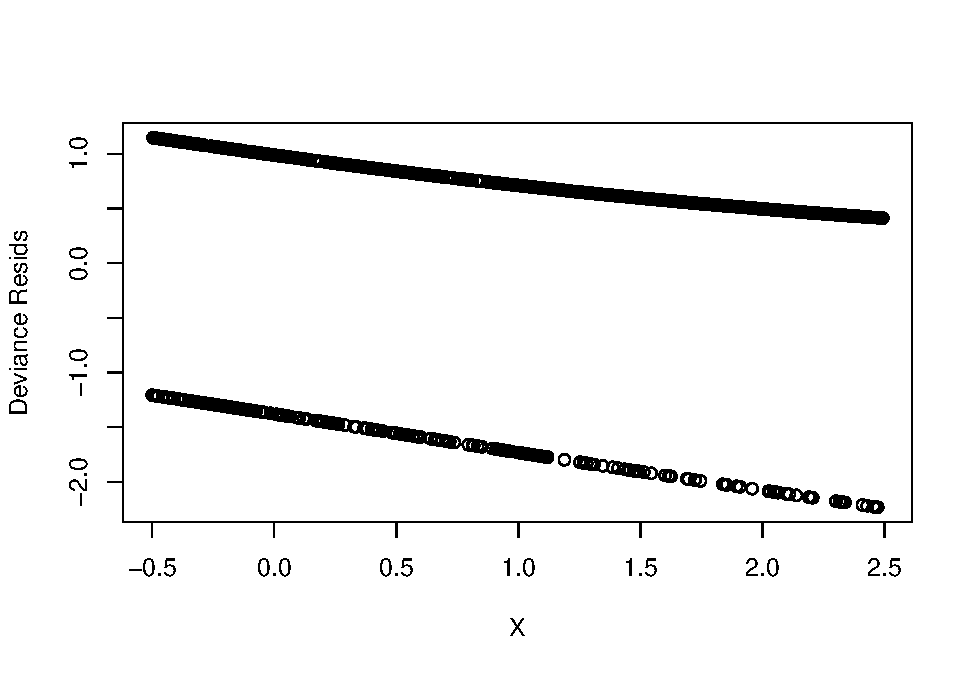
\includegraphics{06-nonlinear_regression_files/figure-latex/unnamed-chunk-33-1.pdf}

However, this plot is not informative. Hence, we can can see the residudals plots that are grouped into bins based on prediction values.

\begin{Shaded}
\begin{Highlighting}[]
\NormalTok{plot\_bin }\OtherTok{\textless{}{-}} \ControlFlowTok{function}\NormalTok{(Y,}
\NormalTok{                     X,}
                     \AttributeTok{bins =} \DecValTok{100}\NormalTok{,}
                     \AttributeTok{return.DF =} \ConstantTok{FALSE}\NormalTok{) \{}
\NormalTok{  Y\_Name }\OtherTok{\textless{}{-}} \FunctionTok{deparse}\NormalTok{(}\FunctionTok{substitute}\NormalTok{(Y))}
\NormalTok{  X\_Name }\OtherTok{\textless{}{-}} \FunctionTok{deparse}\NormalTok{(}\FunctionTok{substitute}\NormalTok{(X))}
\NormalTok{  Binned\_Plot }\OtherTok{\textless{}{-}} \FunctionTok{data.frame}\NormalTok{(}\AttributeTok{Plot\_Y =}\NormalTok{ Y, }\AttributeTok{Plot\_X =}\NormalTok{ X)}
\NormalTok{  Binned\_Plot}\SpecialCharTok{$}\NormalTok{bin }\OtherTok{\textless{}{-}}
    \FunctionTok{cut}\NormalTok{(Binned\_Plot}\SpecialCharTok{$}\NormalTok{Plot\_X, }\AttributeTok{breaks =}\NormalTok{ bins) }\SpecialCharTok{\%\textgreater{}\%}\NormalTok{ as.numeric}
\NormalTok{  Binned\_Plot\_summary }\OtherTok{\textless{}{-}}\NormalTok{ Binned\_Plot }\SpecialCharTok{\%\textgreater{}\%}
    \FunctionTok{group\_by}\NormalTok{(bin) }\SpecialCharTok{\%\textgreater{}\%}
    \FunctionTok{summarise}\NormalTok{(}
      \AttributeTok{Y\_ave =} \FunctionTok{mean}\NormalTok{(Plot\_Y),}
      \AttributeTok{X\_ave =} \FunctionTok{mean}\NormalTok{(Plot\_X),}
      \AttributeTok{Count =} \FunctionTok{n}\NormalTok{()}
\NormalTok{    ) }\SpecialCharTok{\%\textgreater{}\%}\NormalTok{ as.data.frame}
  \FunctionTok{plot}\NormalTok{(}
    \AttributeTok{y =}\NormalTok{ Binned\_Plot\_summary}\SpecialCharTok{$}\NormalTok{Y\_ave,}
    \AttributeTok{x =}\NormalTok{ Binned\_Plot\_summary}\SpecialCharTok{$}\NormalTok{X\_ave,}
    \AttributeTok{ylab =}\NormalTok{ Y\_Name,}
    \AttributeTok{xlab =}\NormalTok{ X\_Name}
\NormalTok{  )}
  \ControlFlowTok{if}\NormalTok{ (return.DF)}
    \FunctionTok{return}\NormalTok{(Binned\_Plot\_summary)}
\NormalTok{\}}
\FunctionTok{plot\_bin}\NormalTok{(}\AttributeTok{Y =}\NormalTok{ Logistic\_Resids,}
         \AttributeTok{X =}\NormalTok{ BinData}\SpecialCharTok{$}\NormalTok{X,}
         \AttributeTok{bins =} \DecValTok{100}\NormalTok{)}
\end{Highlighting}
\end{Shaded}

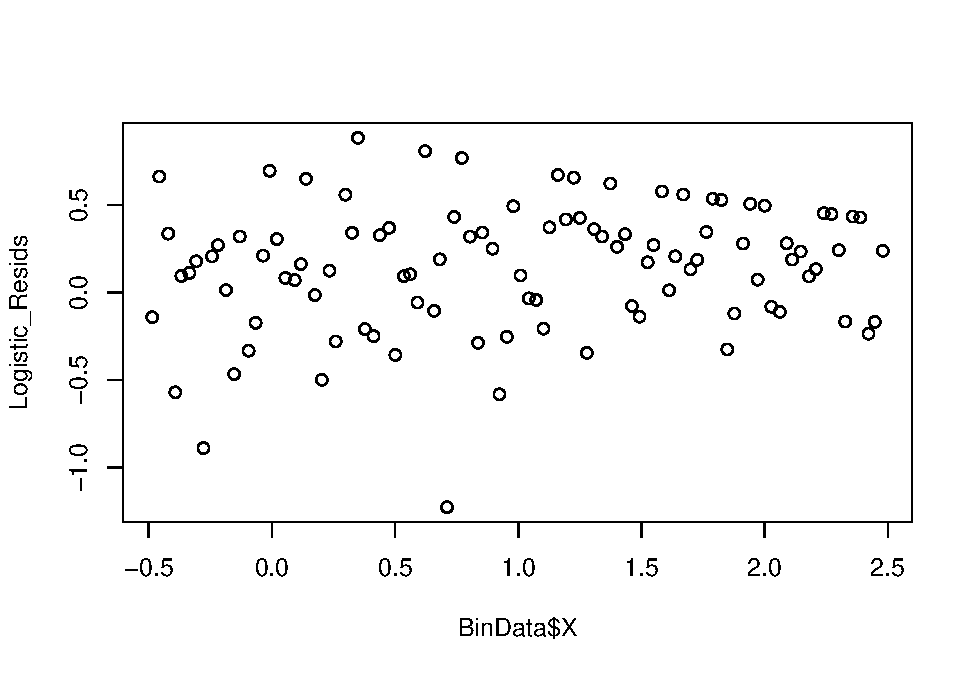
\includegraphics{06-nonlinear_regression_files/figure-latex/unnamed-chunk-34-1.pdf}

We can also see the predicted value against the residuals.

\begin{Shaded}
\begin{Highlighting}[]
\NormalTok{Logistic\_Predictions }\OtherTok{\textless{}{-}} \FunctionTok{predict}\NormalTok{(Logistic\_Model, }\AttributeTok{type =} \StringTok{"response"}\NormalTok{)}
\FunctionTok{plot\_bin}\NormalTok{(}\AttributeTok{Y =}\NormalTok{ Logistic\_Resids, }\AttributeTok{X =}\NormalTok{ Logistic\_Predictions, }\AttributeTok{bins =} \DecValTok{100}\NormalTok{)}
\end{Highlighting}
\end{Shaded}

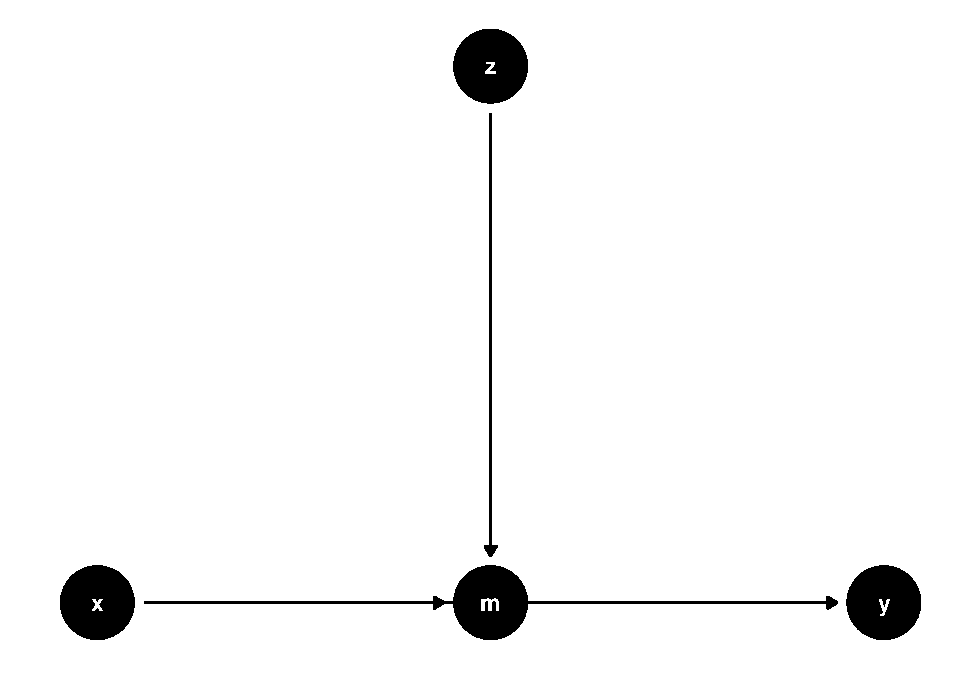
\includegraphics{06-nonlinear_regression_files/figure-latex/unnamed-chunk-35-1.pdf}

We can also look at a binned plot of the logistic prediction versus the true category

\begin{Shaded}
\begin{Highlighting}[]
\NormalTok{NumBins }\OtherTok{\textless{}{-}} \DecValTok{10}
\NormalTok{Binned\_Data }\OtherTok{\textless{}{-}} \FunctionTok{plot\_bin}\NormalTok{(}
  \AttributeTok{Y =}\NormalTok{ BinData}\SpecialCharTok{$}\NormalTok{Y,}
  \AttributeTok{X =}\NormalTok{ Logistic\_Predictions,}
  \AttributeTok{bins =}\NormalTok{ NumBins,}
  \AttributeTok{return.DF =} \ConstantTok{TRUE}
\NormalTok{)}
\NormalTok{Binned\_Data}
\end{Highlighting}
\end{Shaded}

\begin{verbatim}
##    bin     Y_ave     X_ave Count
## 1    1 0.5833333 0.5382095    72
## 2    2 0.5200000 0.5795887    75
## 3    3 0.6567164 0.6156540    67
## 4    4 0.7014925 0.6579674    67
## 5    5 0.6373626 0.6984765    91
## 6    6 0.7500000 0.7373341    72
## 7    7 0.7096774 0.7786747    93
## 8    8 0.8503937 0.8203819   127
## 9    9 0.8947368 0.8601232   133
## 10  10 0.8916256 0.9004734   203
\end{verbatim}

\begin{Shaded}
\begin{Highlighting}[]
\FunctionTok{abline}\NormalTok{(}\DecValTok{0}\NormalTok{, }\DecValTok{1}\NormalTok{, }\AttributeTok{lty =} \DecValTok{2}\NormalTok{, }\AttributeTok{col =} \StringTok{\textquotesingle{}blue\textquotesingle{}}\NormalTok{)}
\end{Highlighting}
\end{Shaded}

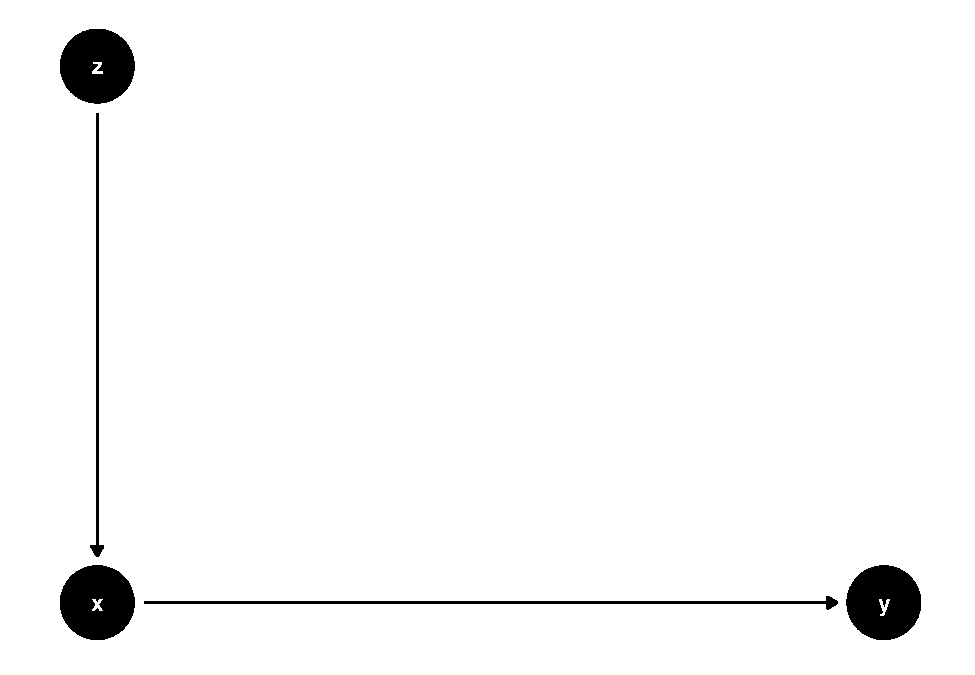
\includegraphics{06-nonlinear_regression_files/figure-latex/unnamed-chunk-36-1.pdf}

\textbf{Formal deviance test}

\textbf{Hosmer-Lemeshow test}

Null hypothesis: the observed events match the expected evens

\[
X^2_{HL} = \sum_{j=1}^{J} \frac{(y_j - m_j \hat{p}_j)^2}{m_j \hat{p}_j(1-\hat{p}_j)}
\]

where

\begin{itemize}
\tightlist
\item
  within the j-th bin, \(y_j\) is the number of successes
\item
  \(m_j\) = number of observations
\item
  \(\hat{p}_j\) = predicted probability
\end{itemize}

Under the null hypothesis, \(X^2_{HLL} \sim \chi^2_{J-1}\)

\begin{Shaded}
\begin{Highlighting}[]
\NormalTok{HL\_BinVals }\OtherTok{\textless{}{-}}
\NormalTok{  (Binned\_Data}\SpecialCharTok{$}\NormalTok{Count }\SpecialCharTok{*}\NormalTok{ Binned\_Data}\SpecialCharTok{$}\NormalTok{Y\_ave }\SpecialCharTok{{-}}\NormalTok{ Binned\_Data}\SpecialCharTok{$}\NormalTok{Count }\SpecialCharTok{*}\NormalTok{ Binned\_Data}\SpecialCharTok{$}\NormalTok{X\_ave) }\SpecialCharTok{\^{}}
  \DecValTok{2} \SpecialCharTok{/}
\NormalTok{  Binned\_Data}\SpecialCharTok{$}\NormalTok{Count }\SpecialCharTok{*}\NormalTok{ Binned\_Data}\SpecialCharTok{$}\NormalTok{X\_ave }\SpecialCharTok{*}\NormalTok{ (}\DecValTok{1} \SpecialCharTok{{-}}\NormalTok{ Binned\_Data}\SpecialCharTok{$}\NormalTok{X\_ave)}
\NormalTok{HLpval }\OtherTok{\textless{}{-}}
  \FunctionTok{pchisq}\NormalTok{(}\AttributeTok{q =} \FunctionTok{sum}\NormalTok{(HL\_BinVals),}
         \AttributeTok{df =}\NormalTok{ NumBins,}
         \AttributeTok{lower.tail =} \ConstantTok{FALSE}\NormalTok{)}
\NormalTok{HLpval}
\end{Highlighting}
\end{Shaded}

\begin{verbatim}
## [1] 0.9999989
\end{verbatim}

Since p-value = 0.99, we do not reject the null hypothesis (i.e., the model is fitting well).

\hypertarget{probit-regression}{%
\section{Probit Regression}\label{probit-regression}}

\[
E(Y_i) = p_i = \Phi(\mathbf{x_i'\theta})
\]

where \(\Phi()\) is the CDF of a N(0,1) random variable.

Other models (e..g, t--distribution; log-log; I complimentary log-log)

We let \(Y_i = 1\) success, \(Y_i =0\) no success. We assume \(Y \sim Ber\) and \(p_i = P(Y_i =1)\), the success probability. We cosnider a logistic regression with the response function \(logit(p_i) = x'_i \beta\)

\textbf{Confusion matrix}

\begin{longtable}[]{@{}lll@{}}
\toprule
& Predicted &\tabularnewline
\midrule
\endhead
Truth & 1 & 0\tabularnewline
1 & True Positive (TP) & False Negative (FN)\tabularnewline
0 & False Positive (FP) & True Negative (TN)\tabularnewline
\bottomrule
\end{longtable}

Sensitivity: ability to identify positive results

\[
\text{Sensitivity} = \frac{TP}{TP + FN}
\]

Specificity: ability to identify negative results

\[
\text{Specificity} = \frac{TN}{TN + FP}
\]

False positive rate: Type I error (1- specificity)

\[
\text{ False Positive Rate} = \frac{FP}{TN+ FP}
\]

False Negative Rate: Type II error (1-sensitivity)

\[
\text{False Negative Rate} = \frac{FN}{TP + FN}
\]

\begin{longtable}[]{@{}lll@{}}
\toprule
& Predicted &\tabularnewline
\midrule
\endhead
Truth & 1 & 0\tabularnewline
1 & Sensitivity & False Negative Rate\tabularnewline
0 & False Positive Rate & Specificity\tabularnewline
\bottomrule
\end{longtable}

\hypertarget{binomial-regression}{%
\section{Binomial Regression}\label{binomial-regression}}

\textbf{Binomial}

Here, cancer case = successes, and control case = failures.

\begin{Shaded}
\begin{Highlighting}[]
\FunctionTok{data}\NormalTok{(}\StringTok{"esoph"}\NormalTok{)}
\FunctionTok{head}\NormalTok{(esoph, }\AttributeTok{n =} \DecValTok{3}\NormalTok{)}
\end{Highlighting}
\end{Shaded}

\begin{verbatim}
##   agegp     alcgp    tobgp ncases ncontrols
## 1 25-34 0-39g/day 0-9g/day      0        40
## 2 25-34 0-39g/day    10-19      0        10
## 3 25-34 0-39g/day    20-29      0         6
\end{verbatim}

\begin{Shaded}
\begin{Highlighting}[]
\FunctionTok{plot}\NormalTok{(}
\NormalTok{  esoph}\SpecialCharTok{$}\NormalTok{ncases }\SpecialCharTok{/}\NormalTok{ (esoph}\SpecialCharTok{$}\NormalTok{ncases }\SpecialCharTok{+}\NormalTok{ esoph}\SpecialCharTok{$}\NormalTok{ncontrols) }\SpecialCharTok{\textasciitilde{}}\NormalTok{ esoph}\SpecialCharTok{$}\NormalTok{alcgp,}
  \AttributeTok{ylab =} \StringTok{"Proportion"}\NormalTok{,}
  \AttributeTok{xlab =} \StringTok{\textquotesingle{}Alcohol consumption\textquotesingle{}}\NormalTok{,}
  \AttributeTok{main =} \StringTok{\textquotesingle{}Esophageal Cancer data\textquotesingle{}}
\NormalTok{)}
\end{Highlighting}
\end{Shaded}

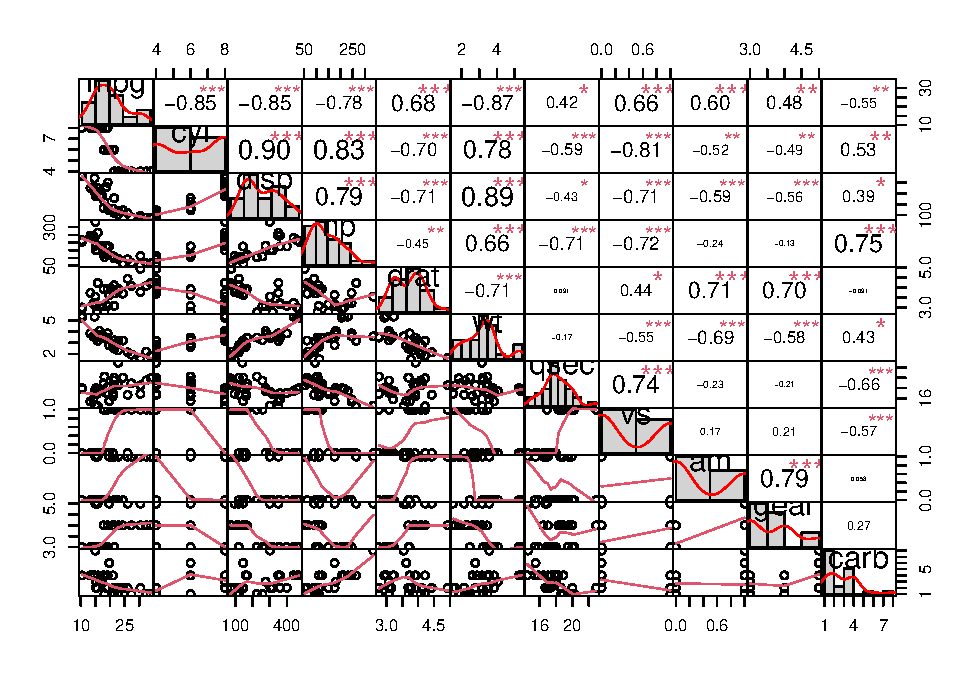
\includegraphics{06-nonlinear_regression_files/figure-latex/unnamed-chunk-38-1.pdf}

\begin{Shaded}
\begin{Highlighting}[]
\FunctionTok{class}\NormalTok{(esoph}\SpecialCharTok{$}\NormalTok{agegp) }\OtherTok{\textless{}{-}} \StringTok{"factor"}
\FunctionTok{class}\NormalTok{(esoph}\SpecialCharTok{$}\NormalTok{alcgp) }\OtherTok{\textless{}{-}} \StringTok{"factor"}
\FunctionTok{class}\NormalTok{(esoph}\SpecialCharTok{$}\NormalTok{tobgp) }\OtherTok{\textless{}{-}} \StringTok{"factor"}
\end{Highlighting}
\end{Shaded}

\begin{Shaded}
\begin{Highlighting}[]
\CommentTok{\#  only the alcohol consumption as a predictor}
\NormalTok{model }\OtherTok{\textless{}{-}} \FunctionTok{glm}\NormalTok{(}\FunctionTok{cbind}\NormalTok{(ncases, ncontrols) }\SpecialCharTok{\textasciitilde{}}\NormalTok{ alcgp, }\AttributeTok{data =}\NormalTok{ esoph, }\AttributeTok{family =}\NormalTok{ binomial)}
\FunctionTok{summary}\NormalTok{(model)}
\end{Highlighting}
\end{Shaded}

\begin{verbatim}
## 
## Call:
## glm(formula = cbind(ncases, ncontrols) ~ alcgp, family = binomial, 
##     data = esoph)
## 
## Deviance Residuals: 
##     Min       1Q   Median       3Q      Max  
## -3.6629  -1.0478  -0.0081   0.6307   3.0296  
## 
## Coefficients:
##             Estimate Std. Error z value Pr(>|z|)    
## (Intercept)  -2.6610     0.1921 -13.854  < 2e-16 ***
## alcgp40-79    1.1064     0.2303   4.804 1.56e-06 ***
## alcgp80-119   1.6656     0.2525   6.597 4.20e-11 ***
## alcgp120+     2.2630     0.2721   8.317  < 2e-16 ***
## ---
## Signif. codes:  0 '***' 0.001 '**' 0.01 '*' 0.05 '.' 0.1 ' ' 1
## 
## (Dispersion parameter for binomial family taken to be 1)
## 
##     Null deviance: 227.24  on 87  degrees of freedom
## Residual deviance: 138.79  on 84  degrees of freedom
## AIC: 294.27
## 
## Number of Fisher Scoring iterations: 5
\end{verbatim}

\begin{Shaded}
\begin{Highlighting}[]
\CommentTok{\#Coefficient Odds}
\FunctionTok{coefficients}\NormalTok{(model) }\SpecialCharTok{\%\textgreater{}\%}\NormalTok{ exp}
\end{Highlighting}
\end{Shaded}

\begin{verbatim}
## (Intercept)  alcgp40-79 alcgp80-119   alcgp120+ 
##  0.06987952  3.02331229  5.28860570  9.61142563
\end{verbatim}

\begin{Shaded}
\begin{Highlighting}[]
\FunctionTok{deviance}\NormalTok{(model)}\SpecialCharTok{/}\FunctionTok{df.residual}\NormalTok{(model)}
\end{Highlighting}
\end{Shaded}

\begin{verbatim}
## [1] 1.652253
\end{verbatim}

\begin{Shaded}
\begin{Highlighting}[]
\NormalTok{model}\SpecialCharTok{$}\NormalTok{aic}
\end{Highlighting}
\end{Shaded}

\begin{verbatim}
## [1] 294.27
\end{verbatim}

\begin{Shaded}
\begin{Highlighting}[]
\CommentTok{\# alcohol consumption and age as predictors}
\NormalTok{better\_model }\OtherTok{\textless{}{-}} \FunctionTok{glm}\NormalTok{(}\FunctionTok{cbind}\NormalTok{(ncases, ncontrols) }\SpecialCharTok{\textasciitilde{}}\NormalTok{ agegp }\SpecialCharTok{+}\NormalTok{ alcgp, }\AttributeTok{data =}\NormalTok{ esoph, }\AttributeTok{family =}\NormalTok{ binomial)}
\FunctionTok{summary}\NormalTok{(better\_model)}
\end{Highlighting}
\end{Shaded}

\begin{verbatim}
## 
## Call:
## glm(formula = cbind(ncases, ncontrols) ~ agegp + alcgp, family = binomial, 
##     data = esoph)
## 
## Deviance Residuals: 
##     Min       1Q   Median       3Q      Max  
## -1.8979  -0.5592  -0.1995   0.5029   2.6250  
## 
## Coefficients:
##             Estimate Std. Error z value Pr(>|z|)    
## (Intercept)  -5.6180     1.0217  -5.499 3.82e-08 ***
## agegp35-44    1.5376     1.0646   1.444 0.148669    
## agegp45-54    2.9470     1.0217   2.884 0.003922 ** 
## agegp55-64    3.3116     1.0172   3.255 0.001132 ** 
## agegp65-74    3.5774     1.0209   3.504 0.000458 ***
## agegp75+      3.5858     1.0620   3.377 0.000734 ***
## alcgp40-79    1.1392     0.2367   4.814 1.48e-06 ***
## alcgp80-119   1.4951     0.2600   5.749 8.97e-09 ***
## alcgp120+     2.2228     0.2843   7.820 5.29e-15 ***
## ---
## Signif. codes:  0 '***' 0.001 '**' 0.01 '*' 0.05 '.' 0.1 ' ' 1
## 
## (Dispersion parameter for binomial family taken to be 1)
## 
##     Null deviance: 227.241  on 87  degrees of freedom
## Residual deviance:  64.572  on 79  degrees of freedom
## AIC: 230.05
## 
## Number of Fisher Scoring iterations: 6
\end{verbatim}

\begin{Shaded}
\begin{Highlighting}[]
\NormalTok{better\_model}\SpecialCharTok{$}\NormalTok{aic }\CommentTok{\#smaller AIC is better}
\end{Highlighting}
\end{Shaded}

\begin{verbatim}
## [1] 230.0526
\end{verbatim}

\begin{Shaded}
\begin{Highlighting}[]
\FunctionTok{coefficients}\NormalTok{(better\_model) }\SpecialCharTok{\%\textgreater{}\%}\NormalTok{ exp}
\end{Highlighting}
\end{Shaded}

\begin{verbatim}
##  (Intercept)   agegp35-44   agegp45-54   agegp55-64   agegp65-74     agegp75+ 
##  0.003631855  4.653273722 19.047899816 27.428640745 35.780787582 36.082010052 
##   alcgp40-79  alcgp80-119    alcgp120+ 
##  3.124334222  4.459579378  9.233256747
\end{verbatim}

\begin{Shaded}
\begin{Highlighting}[]
\FunctionTok{pchisq}\NormalTok{(}
    \AttributeTok{q =}\NormalTok{ model}\SpecialCharTok{$}\NormalTok{deviance }\SpecialCharTok{{-}}\NormalTok{ better\_model}\SpecialCharTok{$}\NormalTok{deviance,}
    \AttributeTok{df =}\NormalTok{ model}\SpecialCharTok{$}\NormalTok{df.residual }\SpecialCharTok{{-}}\NormalTok{ better\_model}\SpecialCharTok{$}\NormalTok{df.residual,}
    \AttributeTok{lower =} \ConstantTok{FALSE}
\NormalTok{)}
\end{Highlighting}
\end{Shaded}

\begin{verbatim}
## [1] 1.354906e-14
\end{verbatim}

\begin{Shaded}
\begin{Highlighting}[]
\CommentTok{\# specify link function as probit}
\NormalTok{Prob\_better\_model }\OtherTok{\textless{}{-}} \FunctionTok{glm}\NormalTok{(}
    \FunctionTok{cbind}\NormalTok{(ncases, ncontrols) }\SpecialCharTok{\textasciitilde{}}\NormalTok{ agegp }\SpecialCharTok{+}\NormalTok{ alcgp,}
    \AttributeTok{data =}\NormalTok{ esoph,}
    \AttributeTok{family =} \FunctionTok{binomial}\NormalTok{(}\AttributeTok{link =}\NormalTok{ probit)}
\NormalTok{)}
\FunctionTok{summary}\NormalTok{(Prob\_better\_model)}
\end{Highlighting}
\end{Shaded}

\begin{verbatim}
## 
## Call:
## glm(formula = cbind(ncases, ncontrols) ~ agegp + alcgp, family = binomial(link = probit), 
##     data = esoph)
## 
## Deviance Residuals: 
##     Min       1Q   Median       3Q      Max  
## -1.8676  -0.5938  -0.1802   0.4852   2.6056  
## 
## Coefficients:
##             Estimate Std. Error z value Pr(>|z|)    
## (Intercept)  -2.9800     0.4291  -6.945 3.79e-12 ***
## agegp35-44    0.6991     0.4491   1.557 0.119520    
## agegp45-54    1.4212     0.4292   3.311 0.000929 ***
## agegp55-64    1.6512     0.4262   3.874 0.000107 ***
## agegp65-74    1.8039     0.4297   4.198 2.69e-05 ***
## agegp75+      1.8025     0.4613   3.908 9.32e-05 ***
## alcgp40-79    0.6224     0.1247   4.990 6.03e-07 ***
## alcgp80-119   0.8256     0.1418   5.823 5.80e-09 ***
## alcgp120+     1.2839     0.1596   8.043 8.77e-16 ***
## ---
## Signif. codes:  0 '***' 0.001 '**' 0.01 '*' 0.05 '.' 0.1 ' ' 1
## 
## (Dispersion parameter for binomial family taken to be 1)
## 
##     Null deviance: 227.241  on 87  degrees of freedom
## Residual deviance:  61.938  on 79  degrees of freedom
## AIC: 227.42
## 
## Number of Fisher Scoring iterations: 6
\end{verbatim}

\hypertarget{poisson-regression}{%
\section{Poisson Regression}\label{poisson-regression}}

From the Poisson distribution

\[
f(Y_i) = \frac{\mu_i^{Y_i}exp(-\mu_i)}{Y_i!}, Y_i = 0,1,.. \\
E(Y_i) = \mu_i  \\
var(Y_i) = \mu_i
\]

which is a natural distribution for counts. We can see that the variance is a function of the mean. If we let \(\mu_i = f(\mathbf{x_i; \theta})\), it would be similar to \protect\hyperlink{logistic-regression-1}{Logistic Regression} since we can choose \(f()\) as \(\mu_i = \mathbf{x_i'\theta}, \mu_i = \exp(\mathbf{x_i'\theta}), \mu_i = \log(\mathbf{x_i'\theta})\)

\hypertarget{application-4}{%
\subsection{Application}\label{application-4}}

Count Data and Poisson regression

\begin{Shaded}
\begin{Highlighting}[]
\FunctionTok{data}\NormalTok{(bioChemists, }\AttributeTok{package =} \StringTok{"pscl"}\NormalTok{)}
\NormalTok{bioChemists }\OtherTok{\textless{}{-}}\NormalTok{ bioChemists }\SpecialCharTok{\%\textgreater{}\%}
    \FunctionTok{rename}\NormalTok{(}
        \AttributeTok{Num\_Article =}\NormalTok{ art, }\CommentTok{\#articles in last 3 years of PhD}
        \AttributeTok{Sex =}\NormalTok{ fem, }\CommentTok{\#coded 1 if female}
        \AttributeTok{Married =}\NormalTok{ mar, }\CommentTok{\#coded 1 if married}
        \AttributeTok{Num\_Kid5 =}\NormalTok{ kid5, }\CommentTok{\#number of childeren under age 6}
        \AttributeTok{PhD\_Quality =}\NormalTok{ phd, }\CommentTok{\#prestige of PhD program}
        \AttributeTok{Num\_MentArticle =}\NormalTok{ ment }\CommentTok{\#articles by mentor in last 3 years}
\NormalTok{    )}
\FunctionTok{hist}\NormalTok{(bioChemists}\SpecialCharTok{$}\NormalTok{Num\_Article, }\AttributeTok{breaks =} \DecValTok{25}\NormalTok{, }\AttributeTok{main =} \StringTok{\textquotesingle{}Number of Articles\textquotesingle{}}\NormalTok{)}
\end{Highlighting}
\end{Shaded}

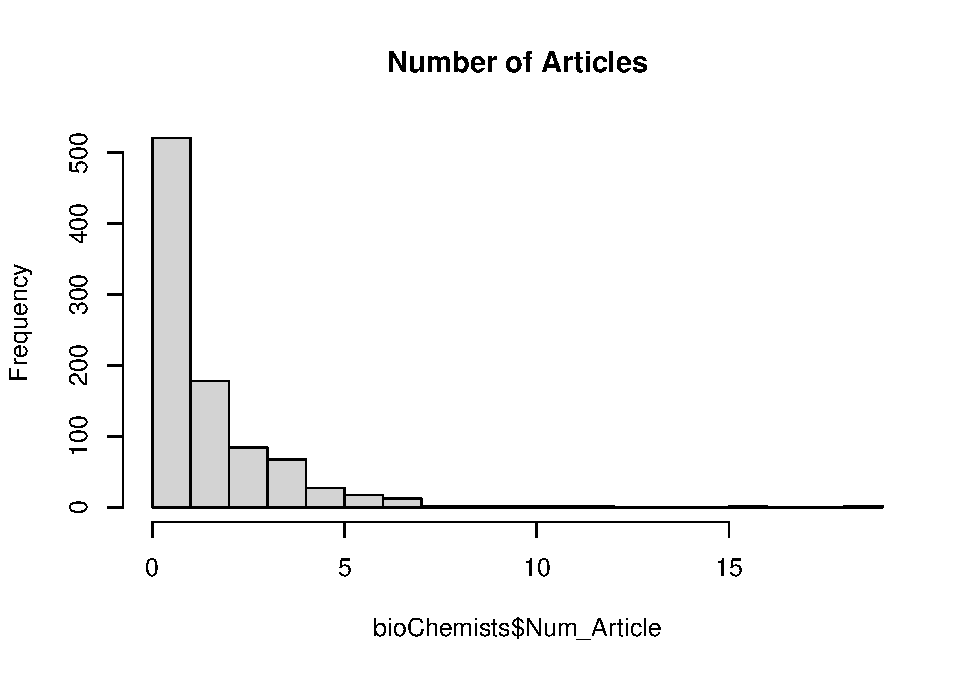
\includegraphics{06-nonlinear_regression_files/figure-latex/unnamed-chunk-44-1.pdf}

\begin{Shaded}
\begin{Highlighting}[]
\NormalTok{Poisson\_Mod }\OtherTok{\textless{}{-}} \FunctionTok{glm}\NormalTok{(Num\_Article }\SpecialCharTok{\textasciitilde{}}\NormalTok{ ., }\AttributeTok{family=}\NormalTok{poisson, bioChemists)}
\FunctionTok{summary}\NormalTok{(Poisson\_Mod)}
\end{Highlighting}
\end{Shaded}

\begin{verbatim}
## 
## Call:
## glm(formula = Num_Article ~ ., family = poisson, data = bioChemists)
## 
## Deviance Residuals: 
##     Min       1Q   Median       3Q      Max  
## -3.5672  -1.5398  -0.3660   0.5722   5.4467  
## 
## Coefficients:
##                  Estimate Std. Error z value Pr(>|z|)    
## (Intercept)      0.304617   0.102981   2.958   0.0031 ** 
## SexWomen        -0.224594   0.054613  -4.112 3.92e-05 ***
## MarriedMarried   0.155243   0.061374   2.529   0.0114 *  
## Num_Kid5        -0.184883   0.040127  -4.607 4.08e-06 ***
## PhD_Quality      0.012823   0.026397   0.486   0.6271    
## Num_MentArticle  0.025543   0.002006  12.733  < 2e-16 ***
## ---
## Signif. codes:  0 '***' 0.001 '**' 0.01 '*' 0.05 '.' 0.1 ' ' 1
## 
## (Dispersion parameter for poisson family taken to be 1)
## 
##     Null deviance: 1817.4  on 914  degrees of freedom
## Residual deviance: 1634.4  on 909  degrees of freedom
## AIC: 3314.1
## 
## Number of Fisher Scoring iterations: 5
\end{verbatim}

Residual of 1634 with 909 df isn't great.

We see Pearson \(\chi^2\)

\begin{Shaded}
\begin{Highlighting}[]
\NormalTok{Predicted\_Means }\OtherTok{\textless{}{-}} \FunctionTok{predict}\NormalTok{(Poisson\_Mod,}\AttributeTok{type =} \StringTok{"response"}\NormalTok{)}
\NormalTok{X2 }\OtherTok{\textless{}{-}} \FunctionTok{sum}\NormalTok{((bioChemists}\SpecialCharTok{$}\NormalTok{Num\_Article }\SpecialCharTok{{-}}\NormalTok{ Predicted\_Means)}\SpecialCharTok{\^{}}\DecValTok{2}\SpecialCharTok{/}\NormalTok{Predicted\_Means)}
\NormalTok{X2}
\end{Highlighting}
\end{Shaded}

\begin{verbatim}
## [1] 1662.547
\end{verbatim}

\begin{Shaded}
\begin{Highlighting}[]
\FunctionTok{pchisq}\NormalTok{(X2,Poisson\_Mod}\SpecialCharTok{$}\NormalTok{df.residual, }\AttributeTok{lower.tail =} \ConstantTok{FALSE}\NormalTok{)}
\end{Highlighting}
\end{Shaded}

\begin{verbatim}
## [1] 7.849882e-47
\end{verbatim}

With interaction terms, there are some improvements

\begin{Shaded}
\begin{Highlighting}[]
\NormalTok{Poisson\_Mod\_All2way }\OtherTok{\textless{}{-}} \FunctionTok{glm}\NormalTok{(Num\_Article }\SpecialCharTok{\textasciitilde{}}\NormalTok{ .}\SpecialCharTok{\^{}}\DecValTok{2}\NormalTok{, }\AttributeTok{family=}\NormalTok{poisson, bioChemists)}
\NormalTok{Poisson\_Mod\_All3way }\OtherTok{\textless{}{-}} \FunctionTok{glm}\NormalTok{(Num\_Article }\SpecialCharTok{\textasciitilde{}}\NormalTok{ .}\SpecialCharTok{\^{}}\DecValTok{3}\NormalTok{, }\AttributeTok{family=}\NormalTok{poisson, bioChemists)}
\end{Highlighting}
\end{Shaded}

Consider the \(\hat{\phi} = \frac{\text{deviance}}{df}\)

\begin{Shaded}
\begin{Highlighting}[]
\NormalTok{Poisson\_Mod}\SpecialCharTok{$}\NormalTok{deviance }\SpecialCharTok{/}\NormalTok{ Poisson\_Mod}\SpecialCharTok{$}\NormalTok{df.residual}
\end{Highlighting}
\end{Shaded}

\begin{verbatim}
## [1] 1.797988
\end{verbatim}

This is evidence for over-dispersion. Likely cause is missing variables. And remedies could either be to include more variables or consider random effects.

A quick fix is to force the Poisson Regression to include this value of \(\phi\), and this model is called ``Quasi-Poisson''.

\begin{Shaded}
\begin{Highlighting}[]
\NormalTok{phi\_hat }\OtherTok{=}\NormalTok{ Poisson\_Mod}\SpecialCharTok{$}\NormalTok{deviance}\SpecialCharTok{/}\NormalTok{Poisson\_Mod}\SpecialCharTok{$}\NormalTok{df.residual}
\FunctionTok{summary}\NormalTok{(Poisson\_Mod,}\AttributeTok{dispersion =}\NormalTok{ phi\_hat)}
\end{Highlighting}
\end{Shaded}

\begin{verbatim}
## 
## Call:
## glm(formula = Num_Article ~ ., family = poisson, data = bioChemists)
## 
## Deviance Residuals: 
##     Min       1Q   Median       3Q      Max  
## -3.5672  -1.5398  -0.3660   0.5722   5.4467  
## 
## Coefficients:
##                 Estimate Std. Error z value Pr(>|z|)    
## (Intercept)      0.30462    0.13809   2.206  0.02739 *  
## SexWomen        -0.22459    0.07323  -3.067  0.00216 ** 
## MarriedMarried   0.15524    0.08230   1.886  0.05924 .  
## Num_Kid5        -0.18488    0.05381  -3.436  0.00059 ***
## PhD_Quality      0.01282    0.03540   0.362  0.71715    
## Num_MentArticle  0.02554    0.00269   9.496  < 2e-16 ***
## ---
## Signif. codes:  0 '***' 0.001 '**' 0.01 '*' 0.05 '.' 0.1 ' ' 1
## 
## (Dispersion parameter for poisson family taken to be 1.797988)
## 
##     Null deviance: 1817.4  on 914  degrees of freedom
## Residual deviance: 1634.4  on 909  degrees of freedom
## AIC: 3314.1
## 
## Number of Fisher Scoring iterations: 5
\end{verbatim}

Or directly rerun the model as

\begin{Shaded}
\begin{Highlighting}[]
\NormalTok{quasiPoisson\_Mod }\OtherTok{\textless{}{-}} \FunctionTok{glm}\NormalTok{(Num\_Article }\SpecialCharTok{\textasciitilde{}}\NormalTok{ ., }\AttributeTok{family=}\NormalTok{quasipoisson, bioChemists)}
\end{Highlighting}
\end{Shaded}

Quasi-Poisson is not recommended, but \protect\hyperlink{negative-binomial-regression}{Negative Binomial Regression} that has an extra parameter to account for over-dispersion is.

\hypertarget{negative-binomial-regression}{%
\section{Negative Binomial Regression}\label{negative-binomial-regression}}

\begin{Shaded}
\begin{Highlighting}[]
\FunctionTok{library}\NormalTok{(MASS)}
\NormalTok{NegBinom\_Mod }\OtherTok{\textless{}{-}}\NormalTok{ MASS}\SpecialCharTok{::}\FunctionTok{glm.nb}\NormalTok{(Num\_Article }\SpecialCharTok{\textasciitilde{}}\NormalTok{ .,bioChemists)}
\FunctionTok{summary}\NormalTok{(NegBinom\_Mod)}
\end{Highlighting}
\end{Shaded}

\begin{verbatim}
## 
## Call:
## MASS::glm.nb(formula = Num_Article ~ ., data = bioChemists, init.theta = 2.264387695, 
##     link = log)
## 
## Deviance Residuals: 
##     Min       1Q   Median       3Q      Max  
## -2.1678  -1.3617  -0.2806   0.4476   3.4524  
## 
## Coefficients:
##                  Estimate Std. Error z value Pr(>|z|)    
## (Intercept)      0.256144   0.137348   1.865 0.062191 .  
## SexWomen        -0.216418   0.072636  -2.979 0.002887 ** 
## MarriedMarried   0.150489   0.082097   1.833 0.066791 .  
## Num_Kid5        -0.176415   0.052813  -3.340 0.000837 ***
## PhD_Quality      0.015271   0.035873   0.426 0.670326    
## Num_MentArticle  0.029082   0.003214   9.048  < 2e-16 ***
## ---
## Signif. codes:  0 '***' 0.001 '**' 0.01 '*' 0.05 '.' 0.1 ' ' 1
## 
## (Dispersion parameter for Negative Binomial(2.2644) family taken to be 1)
## 
##     Null deviance: 1109.0  on 914  degrees of freedom
## Residual deviance: 1004.3  on 909  degrees of freedom
## AIC: 3135.9
## 
## Number of Fisher Scoring iterations: 1
## 
## 
##               Theta:  2.264 
##           Std. Err.:  0.271 
## 
##  2 x log-likelihood:  -3121.917
\end{verbatim}

We can see the dispersion is 2.264 with SE = 0.271, which is significantly different from 1, indicating overdispersion. Check \protect\hyperlink{over-dispersion}{Over-Dispersion} for more detail

\hypertarget{multinomial}{%
\section{Multinomial}\label{multinomial}}

If we have more than two categories or groups that we want to model relative to covariates (e.g., we have observations \(i = 1,…,n\) and groups/ covariates \(j = 1,2,…,J\)), multinomial is our candidate model

Let

\begin{itemize}
\tightlist
\item
  \(p_{ij}\) be the probability that the i-th observation belongs to the j-th group
\item
  \(Y_{ij}\) be the number of observations for individual i in group j; An individual will have observations \(Y_{i1},Y_{i2},…Y_{iJ}\)
\item
  assume the probability of observing this response is given by a multinomial distribution in terms of probabilities \(p_{ij}\), where \(\sum_{j = 1}^J p_{ij} = 1\) . For interpretation, we have a baseline category \(p_{i1} = 1 - \sum_{j = 2}^J p_{ij}\)
\end{itemize}

The link between the mean response (probability) \(p_{ij}\) and a linear function of the covariates

\[
\eta_{ij} = \mathbf{x'_i \beta_j} = \log \frac{p_{ij}}{p_{i1}}, j = 2,..,J
\]

We compare \(p_{ij}\) to the baseline \(p_{i1}\), suggesting

\[
p_{ij} = \frac{\exp(\eta_{ij})}{1 + \sum_{i=2}^J \exp(\eta_{ij})}
\]

which is known as \textbf{multinomial logistic} model.

Note:

\begin{itemize}
\tightlist
\item
  Softmax coding for multinomial logistic regression: rather than selecting a baseline class, we treat all K class symmetrically - euqllay important (no baseline).
\end{itemize}

\[
P(Y = k | X = x) = \frac{exp(\beta_{k1} + \dots + \beta_{k_p x_p})}{\sum_{l = 1}^K exp(\beta_{l0} + \dots + \beta_{l_p x_p})}
\]

then the log odds ratio between k-th and k'-th classes is

\[
\log (\frac{P(Y=k|X=x)}{P(Y = k' | X=x)}) = (\beta_{k0} - \beta_{k'0}) + \dots + (\beta_{kp} - \beta_{k'p}) x_p
\]

\begin{Shaded}
\begin{Highlighting}[]
\FunctionTok{library}\NormalTok{(faraway)}
\FunctionTok{library}\NormalTok{(dplyr)}
\FunctionTok{data}\NormalTok{(nes96, }\AttributeTok{package=}\StringTok{"faraway"}\NormalTok{)}
\FunctionTok{head}\NormalTok{(nes96,}\DecValTok{3}\NormalTok{)}
\end{Highlighting}
\end{Shaded}

\begin{verbatim}
##   popul TVnews selfLR ClinLR DoleLR     PID age  educ   income    vote
## 1     0      7 extCon extLib    Con  strRep  36    HS $3Kminus    Dole
## 2   190      1 sliLib sliLib sliCon weakDem  20  Coll $3Kminus Clinton
## 3    31      7    Lib    Lib    Con weakDem  24 BAdeg $3Kminus Clinton
\end{verbatim}

We try to understand their political strength

\begin{Shaded}
\begin{Highlighting}[]
\FunctionTok{table}\NormalTok{(nes96}\SpecialCharTok{$}\NormalTok{PID)}
\end{Highlighting}
\end{Shaded}

\begin{verbatim}
## 
##  strDem weakDem  indDem  indind  indRep weakRep  strRep 
##     200     180     108      37      94     150     175
\end{verbatim}

\begin{Shaded}
\begin{Highlighting}[]
\NormalTok{nes96}\SpecialCharTok{$}\NormalTok{Political\_Strength }\OtherTok{\textless{}{-}} \ConstantTok{NA}
\NormalTok{nes96}\SpecialCharTok{$}\NormalTok{Political\_Strength[nes96}\SpecialCharTok{$}\NormalTok{PID }\SpecialCharTok{\%in\%} \FunctionTok{c}\NormalTok{(}\StringTok{"strDem"}\NormalTok{, }\StringTok{"strRep"}\NormalTok{)] }\OtherTok{\textless{}{-}}
  \StringTok{"Strong"}
\NormalTok{nes96}\SpecialCharTok{$}\NormalTok{Political\_Strength[nes96}\SpecialCharTok{$}\NormalTok{PID }\SpecialCharTok{\%in\%} \FunctionTok{c}\NormalTok{(}\StringTok{"weakDem"}\NormalTok{, }\StringTok{"weakRep"}\NormalTok{)] }\OtherTok{\textless{}{-}}
  \StringTok{"Weak"}
\NormalTok{nes96}\SpecialCharTok{$}\NormalTok{Political\_Strength[nes96}\SpecialCharTok{$}\NormalTok{PID }\SpecialCharTok{\%in\%} \FunctionTok{c}\NormalTok{(}\StringTok{"indDem"}\NormalTok{, }\StringTok{"indind"}\NormalTok{, }\StringTok{"indRep"}\NormalTok{)] }\OtherTok{\textless{}{-}}
  \StringTok{"Neutral"}
\NormalTok{nes96 }\SpecialCharTok{\%\textgreater{}\%} \FunctionTok{group\_by}\NormalTok{(Political\_Strength) }\SpecialCharTok{\%\textgreater{}\%} \FunctionTok{summarise}\NormalTok{(}\AttributeTok{Count =} \FunctionTok{n}\NormalTok{())}
\end{Highlighting}
\end{Shaded}

\begin{verbatim}
## # A tibble: 3 x 2
##   Political_Strength Count
##   <chr>              <int>
## 1 Neutral              239
## 2 Strong               375
## 3 Weak                 330
\end{verbatim}

visualize the political strength variable

\begin{Shaded}
\begin{Highlighting}[]
\FunctionTok{library}\NormalTok{(ggplot2)}
\NormalTok{Plot\_DF }\OtherTok{\textless{}{-}}\NormalTok{ nes96 }\SpecialCharTok{\%\textgreater{}\%}
  \FunctionTok{mutate}\NormalTok{(}\AttributeTok{Age\_Grp =} \FunctionTok{cut\_number}\NormalTok{(age, }\DecValTok{4}\NormalTok{)) }\SpecialCharTok{\%\textgreater{}\%}
  \FunctionTok{group\_by}\NormalTok{(Age\_Grp, Political\_Strength) }\SpecialCharTok{\%\textgreater{}\%}
  \FunctionTok{summarise}\NormalTok{(}\AttributeTok{count =} \FunctionTok{n}\NormalTok{()) }\SpecialCharTok{\%\textgreater{}\%}
  \FunctionTok{group\_by}\NormalTok{(Age\_Grp) }\SpecialCharTok{\%\textgreater{}\%}
  \FunctionTok{mutate}\NormalTok{(}\AttributeTok{etotal =} \FunctionTok{sum}\NormalTok{(count), }\AttributeTok{proportion =}\NormalTok{ count }\SpecialCharTok{/}\NormalTok{ etotal)}
\end{Highlighting}
\end{Shaded}

\begin{verbatim}
## `summarise()` has grouped output by 'Age_Grp'. You can override using the `.groups` argument.
\end{verbatim}

\begin{Shaded}
\begin{Highlighting}[]
\NormalTok{Age\_Plot }\OtherTok{\textless{}{-}} \FunctionTok{ggplot}\NormalTok{(}
\NormalTok{  Plot\_DF,}
  \FunctionTok{aes}\NormalTok{(}
    \AttributeTok{x =}\NormalTok{ Age\_Grp,}
    \AttributeTok{y =}\NormalTok{ proportion,}
    \AttributeTok{group =}\NormalTok{ Political\_Strength,}
    \AttributeTok{linetype =}\NormalTok{ Political\_Strength,}
    \AttributeTok{color =}\NormalTok{ Political\_Strength}
\NormalTok{  )}
\NormalTok{) }\SpecialCharTok{+}
  \FunctionTok{geom\_line}\NormalTok{(}\AttributeTok{size =} \DecValTok{2}\NormalTok{)}
\NormalTok{Age\_Plot}
\end{Highlighting}
\end{Shaded}

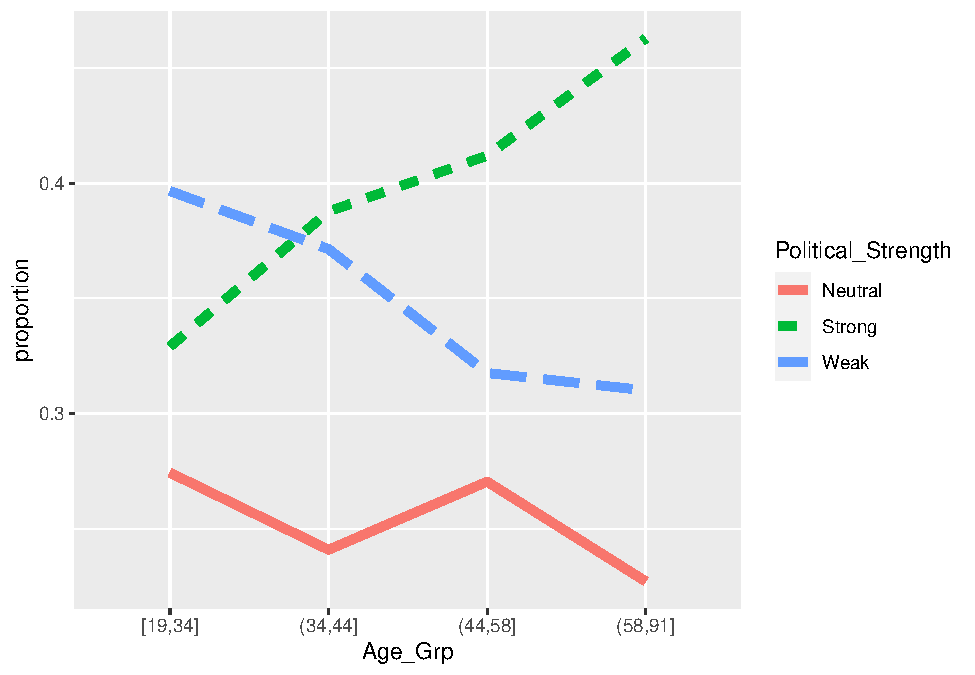
\includegraphics{06-nonlinear_regression_files/figure-latex/unnamed-chunk-54-1.pdf}

Fit the multinomial logistic model:

model political strength as a function of age and education

\begin{Shaded}
\begin{Highlighting}[]
\FunctionTok{library}\NormalTok{(nnet)}
\NormalTok{Multinomial\_Model }\OtherTok{\textless{}{-}}
    \FunctionTok{multinom}\NormalTok{(Political\_Strength }\SpecialCharTok{\textasciitilde{}}\NormalTok{ age }\SpecialCharTok{+}\NormalTok{ educ, nes96, }\AttributeTok{trace =}\NormalTok{ F)}
\FunctionTok{summary}\NormalTok{(Multinomial\_Model)}
\end{Highlighting}
\end{Shaded}

\begin{verbatim}
## Call:
## multinom(formula = Political_Strength ~ age + educ, data = nes96, 
##     trace = F)
## 
## Coefficients:
##        (Intercept)          age     educ.L     educ.Q     educ.C      educ^4
## Strong -0.08788729  0.010700364 -0.1098951 -0.2016197 -0.1757739 -0.02116307
## Weak    0.51976285 -0.004868771 -0.1431104 -0.2405395 -0.2411795  0.18353634
##            educ^5     educ^6
## Strong -0.1664377 -0.1359449
## Weak   -0.1489030 -0.2173144
## 
## Std. Errors:
##        (Intercept)         age    educ.L    educ.Q    educ.C    educ^4
## Strong   0.3017034 0.005280743 0.4586041 0.4318830 0.3628837 0.2964776
## Weak     0.3097923 0.005537561 0.4920736 0.4616446 0.3881003 0.3169149
##           educ^5    educ^6
## Strong 0.2515012 0.2166774
## Weak   0.2643747 0.2199186
## 
## Residual Deviance: 2024.596 
## AIC: 2056.596
\end{verbatim}

Alternatively, stepwise model selection based AIC

\begin{Shaded}
\begin{Highlighting}[]
\NormalTok{Multinomial\_Step }\OtherTok{\textless{}{-}} \FunctionTok{step}\NormalTok{(Multinomial\_Model,}\AttributeTok{trace =} \DecValTok{0}\NormalTok{)}
\end{Highlighting}
\end{Shaded}

\begin{verbatim}
## trying - age 
## trying - educ 
## trying - age
\end{verbatim}

\begin{Shaded}
\begin{Highlighting}[]
\NormalTok{Multinomial\_Step}
\end{Highlighting}
\end{Shaded}

\begin{verbatim}
## Call:
## multinom(formula = Political_Strength ~ age, data = nes96, trace = F)
## 
## Coefficients:
##        (Intercept)          age
## Strong -0.01988977  0.009832916
## Weak    0.59497046 -0.005954348
## 
## Residual Deviance: 2030.756 
## AIC: 2038.756
\end{verbatim}

compare the best model to the full model based on deviance

\begin{Shaded}
\begin{Highlighting}[]
\FunctionTok{pchisq}\NormalTok{(}\AttributeTok{q =} \FunctionTok{deviance}\NormalTok{(Multinomial\_Step) }\SpecialCharTok{{-}} \FunctionTok{deviance}\NormalTok{(Multinomial\_Model),}
\AttributeTok{df =}\NormalTok{ Multinomial\_Model}\SpecialCharTok{$}\NormalTok{edf}\SpecialCharTok{{-}}\NormalTok{Multinomial\_Step}\SpecialCharTok{$}\NormalTok{edf,}\AttributeTok{lower=}\NormalTok{F)}
\end{Highlighting}
\end{Shaded}

\begin{verbatim}
## [1] 0.9078172
\end{verbatim}

We see no significant difference

Plot of the fitted model

\begin{Shaded}
\begin{Highlighting}[]
\NormalTok{PlotData }\OtherTok{\textless{}{-}} \FunctionTok{data.frame}\NormalTok{(}\AttributeTok{age =} \FunctionTok{seq}\NormalTok{(}\AttributeTok{from =} \DecValTok{19}\NormalTok{, }\AttributeTok{to =} \DecValTok{91}\NormalTok{))}
\NormalTok{Preds }\OtherTok{\textless{}{-}}
\NormalTok{  PlotData }\SpecialCharTok{\%\textgreater{}\%} \FunctionTok{bind\_cols}\NormalTok{(}\FunctionTok{data.frame}\NormalTok{(}\FunctionTok{predict}\NormalTok{(}
    \AttributeTok{object =}\NormalTok{ Multinomial\_Step,}
\NormalTok{    PlotData, }\AttributeTok{type =} \StringTok{"probs"}
\NormalTok{  )))}
\FunctionTok{plot}\NormalTok{(}
  \AttributeTok{x =}\NormalTok{ Preds}\SpecialCharTok{$}\NormalTok{age,}
  \AttributeTok{y =}\NormalTok{ Preds}\SpecialCharTok{$}\NormalTok{Neutral,}
  \AttributeTok{type =} \StringTok{"l"}\NormalTok{,}
  \AttributeTok{ylim =} \FunctionTok{c}\NormalTok{(}\FloatTok{0.2}\NormalTok{, }\FloatTok{0.6}\NormalTok{),}
  \AttributeTok{col =} \StringTok{"black"}\NormalTok{,}
  \AttributeTok{ylab =} \StringTok{"Proportion"}\NormalTok{,}
  \AttributeTok{xlab =} \StringTok{"Age"}
\NormalTok{)}
\FunctionTok{lines}\NormalTok{(}\AttributeTok{x =}\NormalTok{ Preds}\SpecialCharTok{$}\NormalTok{age,}
      \AttributeTok{y =}\NormalTok{ Preds}\SpecialCharTok{$}\NormalTok{Weak,}
      \AttributeTok{col =} \StringTok{"blue"}\NormalTok{)}
\FunctionTok{lines}\NormalTok{(}\AttributeTok{x =}\NormalTok{ Preds}\SpecialCharTok{$}\NormalTok{age,}
      \AttributeTok{y =}\NormalTok{ Preds}\SpecialCharTok{$}\NormalTok{Strong,}
      \AttributeTok{col =} \StringTok{"red"}\NormalTok{)}
\FunctionTok{legend}\NormalTok{(}
  \StringTok{\textquotesingle{}topleft\textquotesingle{}}\NormalTok{,}
  \AttributeTok{legend =} \FunctionTok{c}\NormalTok{(}\StringTok{\textquotesingle{}Neutral\textquotesingle{}}\NormalTok{, }\StringTok{\textquotesingle{}Weak\textquotesingle{}}\NormalTok{, }\StringTok{\textquotesingle{}Strong\textquotesingle{}}\NormalTok{),}
  \AttributeTok{col =} \FunctionTok{c}\NormalTok{(}\StringTok{\textquotesingle{}black\textquotesingle{}}\NormalTok{, }\StringTok{\textquotesingle{}blue\textquotesingle{}}\NormalTok{, }\StringTok{\textquotesingle{}red\textquotesingle{}}\NormalTok{),}
  \AttributeTok{lty =} \DecValTok{1}
\NormalTok{)}
\end{Highlighting}
\end{Shaded}

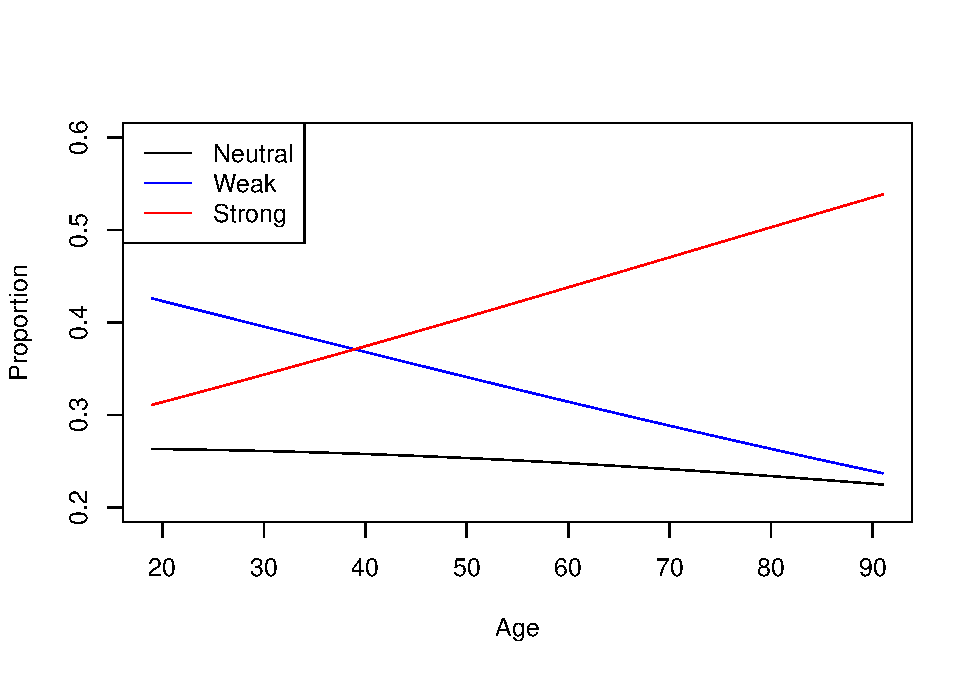
\includegraphics{06-nonlinear_regression_files/figure-latex/unnamed-chunk-58-1.pdf}

\begin{Shaded}
\begin{Highlighting}[]
\FunctionTok{predict}\NormalTok{(Multinomial\_Step,}\FunctionTok{data.frame}\NormalTok{(}\AttributeTok{age =} \DecValTok{34}\NormalTok{)) }\CommentTok{\# predicted result (categoriy of political strength) of 34 year old}
\end{Highlighting}
\end{Shaded}

\begin{verbatim}
## [1] Weak
## Levels: Neutral Strong Weak
\end{verbatim}

\begin{Shaded}
\begin{Highlighting}[]
\FunctionTok{predict}\NormalTok{(Multinomial\_Step,}\FunctionTok{data.frame}\NormalTok{(}\AttributeTok{age =} \FunctionTok{c}\NormalTok{(}\DecValTok{34}\NormalTok{,}\DecValTok{35}\NormalTok{)),}\AttributeTok{type=}\StringTok{"probs"}\NormalTok{) }\CommentTok{\# predicted result of the probabilities of each level of political strength for a 34 and 35}
\end{Highlighting}
\end{Shaded}

\begin{verbatim}
##     Neutral    Strong      Weak
## 1 0.2597275 0.3556910 0.3845815
## 2 0.2594080 0.3587639 0.3818281
\end{verbatim}

If categories are ordered (i.e., ordinal data), we must use another approach (still multinomial, but use cumulative probabilities).

Another example

\begin{Shaded}
\begin{Highlighting}[]
\FunctionTok{library}\NormalTok{(agridat)}
\NormalTok{dat }\OtherTok{\textless{}{-}}\NormalTok{ agridat}\SpecialCharTok{::}\NormalTok{streibig.competition}
\CommentTok{\# See Schaberger and Pierce, pages 370+}
\CommentTok{\# Consider only the mono{-}species barley data (no competition from Sinapis)}
\NormalTok{gammaDat }\OtherTok{\textless{}{-}} \FunctionTok{subset}\NormalTok{(dat, sseeds }\SpecialCharTok{\textless{}} \DecValTok{1}\NormalTok{)}
\NormalTok{gammaDat }\OtherTok{\textless{}{-}}
  \FunctionTok{transform}\NormalTok{(gammaDat,}
            \AttributeTok{x =}\NormalTok{ bseeds,}
            \AttributeTok{y =}\NormalTok{ bdwt,}
            \AttributeTok{block =} \FunctionTok{factor}\NormalTok{(block))}
\CommentTok{\# Inverse yield looks like it will be a good fit for Gamma\textquotesingle{}s inverse link}
\FunctionTok{ggplot}\NormalTok{(gammaDat, }\FunctionTok{aes}\NormalTok{(}\AttributeTok{x =}\NormalTok{ x, }\AttributeTok{y =} \DecValTok{1} \SpecialCharTok{/}\NormalTok{ y)) }\SpecialCharTok{+} \FunctionTok{geom\_point}\NormalTok{(}\FunctionTok{aes}\NormalTok{(}\AttributeTok{color =}\NormalTok{ block, }\AttributeTok{shape =}
\NormalTok{                                                           block)) }\SpecialCharTok{+}
  \FunctionTok{xlab}\NormalTok{(}\StringTok{\textquotesingle{}Seeding Rate\textquotesingle{}}\NormalTok{) }\SpecialCharTok{+} \FunctionTok{ylab}\NormalTok{(}\StringTok{\textquotesingle{}Inverse yield\textquotesingle{}}\NormalTok{) }\SpecialCharTok{+} \FunctionTok{ggtitle}\NormalTok{(}\StringTok{\textquotesingle{}Streibig Competion {-} Barley only\textquotesingle{}}\NormalTok{)}
\end{Highlighting}
\end{Shaded}

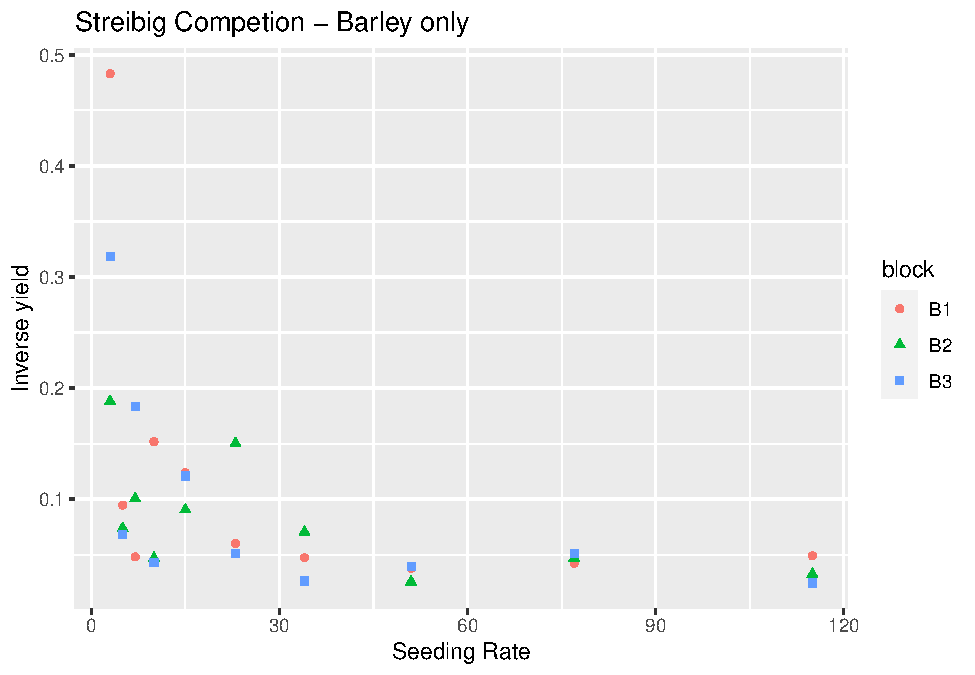
\includegraphics{06-nonlinear_regression_files/figure-latex/unnamed-chunk-60-1.pdf}

\[
Y \sim Gamma
\]

because Gamma is non-negative as opposed to Normal. The canonical Gamma link function is the inverse (or reciprocal) link

\[
\eta_{ij} = \beta_{0j} + \beta_{1j}x_{ij} + \beta_2x_{ij}^2 \\
Y_{ij} = \eta_{ij}^{-1}
\]

The linear predictor is a quadratic model fit to each of the j-th blocks. A different model (not fitted) could be one with common slopes: glm(y \(\sim\) x + I(x\^{}2),\ldots)

\begin{Shaded}
\begin{Highlighting}[]
\CommentTok{\# linear predictor is quadratic, with separate intercept and slope per block}
\NormalTok{m1 }\OtherTok{\textless{}{-}} \FunctionTok{glm}\NormalTok{(y }\SpecialCharTok{\textasciitilde{}}\NormalTok{ block }\SpecialCharTok{+}\NormalTok{ block}\SpecialCharTok{*}\NormalTok{x }\SpecialCharTok{+}\NormalTok{ block}\SpecialCharTok{*}\FunctionTok{I}\NormalTok{(x}\SpecialCharTok{\^{}}\DecValTok{2}\NormalTok{), }\AttributeTok{data=}\NormalTok{gammaDat,}\AttributeTok{family=}\FunctionTok{Gamma}\NormalTok{(}\AttributeTok{link=}\StringTok{"inverse"}\NormalTok{))}
\FunctionTok{summary}\NormalTok{(m1)}
\end{Highlighting}
\end{Shaded}

\begin{verbatim}
## 
## Call:
## glm(formula = y ~ block + block * x + block * I(x^2), family = Gamma(link = "inverse"), 
##     data = gammaDat)
## 
## Deviance Residuals: 
##      Min        1Q    Median        3Q       Max  
## -1.21708  -0.44148   0.02479   0.17999   0.80745  
## 
## Coefficients:
##                  Estimate Std. Error t value Pr(>|t|)    
## (Intercept)     1.115e-01  2.870e-02   3.886 0.000854 ***
## blockB2        -1.208e-02  3.880e-02  -0.311 0.758630    
## blockB3        -2.386e-02  3.683e-02  -0.648 0.524029    
## x              -2.075e-03  1.099e-03  -1.888 0.072884 .  
## I(x^2)          1.372e-05  9.109e-06   1.506 0.146849    
## blockB2:x       5.198e-04  1.468e-03   0.354 0.726814    
## blockB3:x       7.475e-04  1.393e-03   0.537 0.597103    
## blockB2:I(x^2) -5.076e-06  1.184e-05  -0.429 0.672475    
## blockB3:I(x^2) -6.651e-06  1.123e-05  -0.592 0.560012    
## ---
## Signif. codes:  0 '***' 0.001 '**' 0.01 '*' 0.05 '.' 0.1 ' ' 1
## 
## (Dispersion parameter for Gamma family taken to be 0.3232083)
## 
##     Null deviance: 13.1677  on 29  degrees of freedom
## Residual deviance:  7.8605  on 21  degrees of freedom
## AIC: 225.32
## 
## Number of Fisher Scoring iterations: 5
\end{verbatim}

For predict new value of x

\begin{Shaded}
\begin{Highlighting}[]
\NormalTok{newdf }\OtherTok{\textless{}{-}}
  \FunctionTok{expand.grid}\NormalTok{(}\AttributeTok{x =} \FunctionTok{seq}\NormalTok{(}\DecValTok{0}\NormalTok{, }\DecValTok{120}\NormalTok{, }\AttributeTok{length =} \DecValTok{50}\NormalTok{), }\AttributeTok{block =} \FunctionTok{factor}\NormalTok{(}\FunctionTok{c}\NormalTok{(}\StringTok{\textquotesingle{}B1\textquotesingle{}}\NormalTok{, }\StringTok{\textquotesingle{}B2\textquotesingle{}}\NormalTok{, }\StringTok{\textquotesingle{}B3\textquotesingle{}}\NormalTok{)))}
\NormalTok{newdf}\SpecialCharTok{$}\NormalTok{pred }\OtherTok{\textless{}{-}} \FunctionTok{predict}\NormalTok{(m1, }\AttributeTok{new =}\NormalTok{ newdf, }\AttributeTok{type =} \StringTok{\textquotesingle{}response\textquotesingle{}}\NormalTok{)}
\FunctionTok{ggplot}\NormalTok{(gammaDat, }\FunctionTok{aes}\NormalTok{(}\AttributeTok{x =}\NormalTok{ x, }\AttributeTok{y =}\NormalTok{ y)) }\SpecialCharTok{+} \FunctionTok{geom\_point}\NormalTok{(}\FunctionTok{aes}\NormalTok{(}\AttributeTok{color =}\NormalTok{ block, }\AttributeTok{shape =}
\NormalTok{                                                       block)) }\SpecialCharTok{+}
  \FunctionTok{xlab}\NormalTok{(}\StringTok{\textquotesingle{}Seeding Rate\textquotesingle{}}\NormalTok{) }\SpecialCharTok{+} \FunctionTok{ylab}\NormalTok{(}\StringTok{\textquotesingle{}Inverse yield\textquotesingle{}}\NormalTok{) }\SpecialCharTok{+} \FunctionTok{ggtitle}\NormalTok{(}\StringTok{\textquotesingle{}Streibig Competion {-} Barley only Predictions\textquotesingle{}}\NormalTok{) }\SpecialCharTok{+}
  \FunctionTok{geom\_line}\NormalTok{(}\AttributeTok{data =}\NormalTok{ newdf, }\FunctionTok{aes}\NormalTok{(}
    \AttributeTok{x =}\NormalTok{ x,}
    \AttributeTok{y =}\NormalTok{ pred,}
    \AttributeTok{color =}\NormalTok{ block,}
    \AttributeTok{linetype =}\NormalTok{ block}
\NormalTok{  ))}
\end{Highlighting}
\end{Shaded}

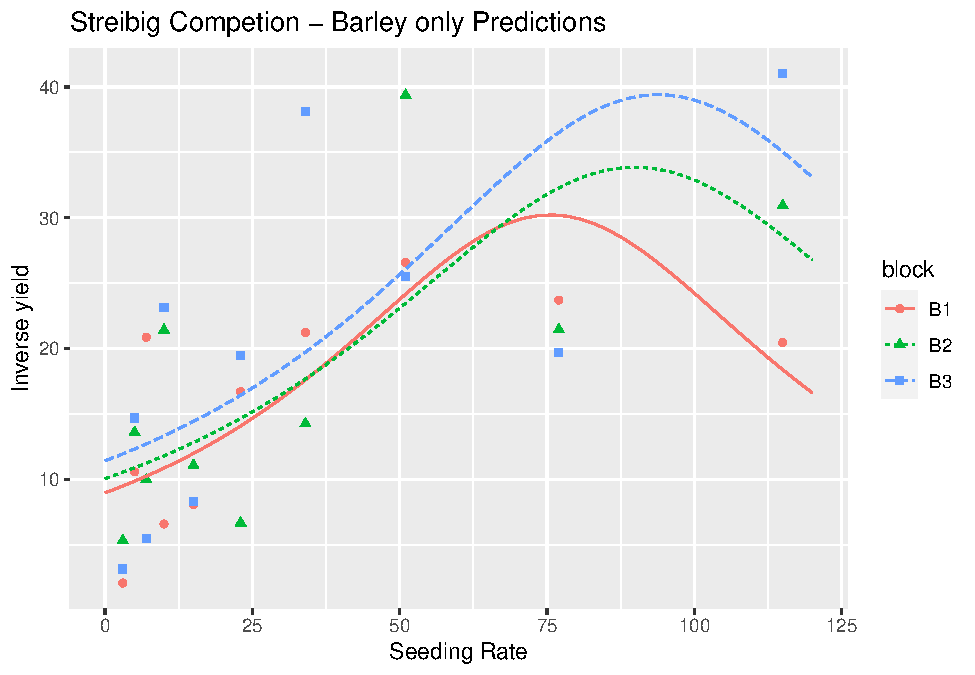
\includegraphics{06-nonlinear_regression_files/figure-latex/unnamed-chunk-62-1.pdf}

\hypertarget{generalization}{%
\section{Generalization}\label{generalization}}

We can see that Poisson regression looks similar to logistic regression. Hence, we can generalize to a class of modeling. Thanks to \citep{Nelder_1972}, we have the \textbf{generalized linear models} (GLMs). Estimation is generalize in these models.

\textbf{Exponential Family}\\
The theory of GLMs is developed for data with distribution given y the \textbf{exponential family}.\\
The form of the data distribution that is useful for GLMs is

\[
f(y;\theta, \phi) = \exp(\frac{\theta y - b(\theta)}{a(\phi)} + c(y, \phi))
\]

where

\begin{itemize}
\tightlist
\item
  \(\theta\) is called the natural parameter
\item
  \(\phi\) is called the dispersion parameter
\end{itemize}

\textbf{Note}:

This family includes the \protect\hyperlink{gamma}{Gamma}, \protect\hyperlink{normal}{Normal}, \protect\hyperlink{poisson}{Poisson}, and other. For all parameterization of the exponential family, check this \href{https://www.stat.purdue.edu/~tlzhang/stat526/logistic.pdf}{link}

\textbf{Example}

if we have \(Y \sim N(\mu, \sigma^2)\)

\[
\begin{aligned}
f(y; \mu, \sigma^2) &= \frac{1}{(2\pi \sigma^2)^{1/2}}\exp(-\frac{1}{2\sigma^2}(y- \mu)^2) \\
&= \exp(-\frac{1}{2\sigma^2}(y^2 - 2y \mu +\mu^2)- \frac{1}{2}\log(2\pi \sigma^2)) \\
&= \exp(\frac{y \mu - \mu^2/2}{\sigma^2} - \frac{y^2}{2\sigma^2} - \frac{1}{2}\log(2\pi \sigma^2)) \\
&= \exp(\frac{\theta y - b(\theta)}{a(\phi)} + c(y , \phi))
\end{aligned}
\]

where

\begin{itemize}
\tightlist
\item
  \(\theta = \mu\)
\item
  \(b(\theta) = \frac{\mu^2}{2}\)
\item
  \(a(\phi) = \sigma^2 = \phi\)
\item
  \(c(y , \phi) = - \frac{1}{2}(\frac{y^2}{\phi}+\log(2\pi \sigma^2))\)
\end{itemize}

\textbf{Properties of GLM exponential families}

\begin{enumerate}
\def\labelenumi{\arabic{enumi}.}
\item
  \(E(Y) = b' (\theta)\) where \(b'(\theta) = \frac{\partial b(\theta)}{\partial \theta}\) (here \texttt{\textquotesingle{}} is ``prime'', not transpose)
\item
  \(var(Y) = a(\phi)b''(\theta)= a(\phi)V(\mu)\).

  \begin{itemize}
  \tightlist
  \item
    \(V(\mu)\) is the \emph{variance function}; however, it is only the variance in the case that \(a(\phi) =1\)
  \end{itemize}
\item
  If \(a(), b(), c()\) are identifiable, we will derive expected value and variance of Y.
\end{enumerate}

Example

Normal distribution

\[
b'(\theta) = \frac{\partial b(\mu^2/2)}{\partial \mu} = \mu \\
V(\mu) = \frac{\partial^2 (\mu^2/2)}{\partial \mu^2} = 1 \\
\to var(Y) = a(\phi) = \sigma^2
\]

Poisson distribution

\[
\begin{aligned}
f(y, \theta, \phi) &= \frac{\mu^y \exp(-\mu)}{y!} \\
&= \exp(y\log(\mu) - \mu - \log(y!)) \\
&= \exp(y\theta - \exp(\theta) - \log(y!))
\end{aligned}
\]

where

\begin{itemize}
\tightlist
\item
  \(\theta = \log(\mu)\)
\item
  \(a(\phi) = 1\)
\item
  \(b(\theta) = \exp(\theta)\)
\item
  \(c(y, \phi) = \log(y!)\)
\end{itemize}

Hence,

\[
E(Y) = \frac{\partial b(\theta)}{\partial \theta} = \exp(\theta) = \mu \\
var(Y) = \frac{\partial^2 b(\theta)}{\partial \theta^2} = \mu
\]

Since \(\mu = E(Y) = b'(\theta)\)

In GLM, we take some monotone function (typically nonlinear) of \(\mu\) to be linear in the set of covariates

\[
g(\mu) = g(b'(\theta)) = \mathbf{x'\beta}
\]

Equivalently,

\[
\mu = g^{-1}(\mathbf{x'\beta})
\]

where \(g(.)\) is the \textbf{link function} since it links mean response (\(\mu = E(Y)\)) and a linear expression of the covariates

Some people use \(\eta = \mathbf{x'\beta}\) where \(\eta\) = the ``linear predictor''

\textbf{GLM is composed of 2 components}

The \textbf{random component}:

\begin{itemize}
\item
  is the distribution chosen to model the response variables \(Y_1,...,Y_n\)
\item
  is specified by the choice fo \(a(), b(), c()\) in the exponential form
\item
  Notation:

  \begin{itemize}
  \tightlist
  \item
    Assume that there are n \textbf{independent} response variables \(Y_1,...,Y_n\) with densities\\
    \[
    f(y_i ; \theta_i, \phi) = \exp(\frac{\theta_i y_i - b(\theta_i)}{a(\phi)}+ c(y_i, \phi))
    \] notice each observation might have different densities
  \item
    Assume that \(\phi\) is constant for all \(i = 1,...,n\), but \(\theta_i\) will vary. \(\mu_i = E(Y_i)\) for all i.
  \end{itemize}
\end{itemize}

The \textbf{systematic component}

\begin{itemize}
\item
  is the portion of the model that gives the relation between \(\mu\) and the covariates \(\mathbf{x}\)
\item
  consists of 2 parts:

  \begin{itemize}
  \tightlist
  \item
    the \emph{link} function, \(g(.)\)
  \item
    the \emph{linear predictor}, \(\eta = \mathbf{x'\beta}\)
  \end{itemize}
\item
  Notation:

  \begin{itemize}
  \tightlist
  \item
    assume \(g(\mu_i) = \mathbf{x'\beta} = \eta_i\) where \(\mathbf{\beta} = (\beta_1,..., \beta_p)'\)
  \item
    The parameters to be estimated are \(\beta_1,...\beta_p , \phi\)
  \end{itemize}
\end{itemize}

\textbf{The Canonical Link}

To choose \(g(.)\), we can use \textbf{canonical link function} (Remember: Canonical link is just a special case of the link function)

If the link function \(g(.)\) is such \(g(\mu_i) = \eta_i = \theta_i\), the natural parameter, then \(g(.)\) is the canonical link.

\begin{verbatim}
## Warning: package 'jpeg' was built under R version 4.0.5
\end{verbatim}

\begin{center}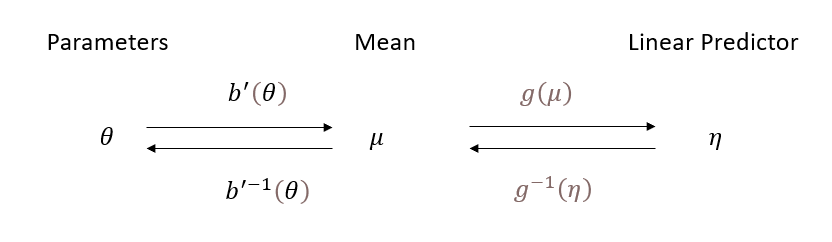
\includegraphics[width=11.56in]{images/GLM} \end{center}

\begin{itemize}
\tightlist
\item
  \(b(\theta)\) = cumulant moment generating function
\item
  \(g(\mu)\) is the link function, which relates the linear predictor to the mean and is required to be monotone increasing, continuously differentiable and invertible.
\end{itemize}

Equivalently, we can think of canonical link function as

\[
\gamma^{-1} \circ g^{-1} = I
\]
which is the identity. Hence,

\[
\theta = \eta
\]

\textbf{The inverse link}

\(g^{-1}(.)\) is also known as the mean function, take linear predictor output (ranging from \(-\infty\) to \(\infty\)) and transform it into a different scale.

\begin{itemize}
\tightlist
\item
  \textbf{Exponential}: converts \(\mathbf{\beta X}\) into a curve that is restricted between 0 and \(\infty\) (which you can see that is useful in case you want to convert a linear predictor into a non-negative value). \(\lambda = \exp(y) = \mathbf{\beta X}\)
\item
  \textbf{Inverse Logit} (also known as logistic): converts \(\mathbf{\beta X}\) into a curve that is restricted between 0 and 1, which is useful in case you want to convert a linear predictor to a probability. \(\theta = \frac{1}{1 + \exp(-y)} = \frac{1}{1 + \exp(- \mathbf{\beta X})}\)

  \begin{itemize}
  \tightlist
  \item
    \(y\) = linear predictor value
  \item
    \(\theta\) = transformed value
  \end{itemize}
\end{itemize}

The \textbf{identity link} is that

\[
\eta_i = g(\mu_i) = \mu_i \\
\mu_i = g^{-1}(\eta_i) = \eta_i
\]

\begin{center}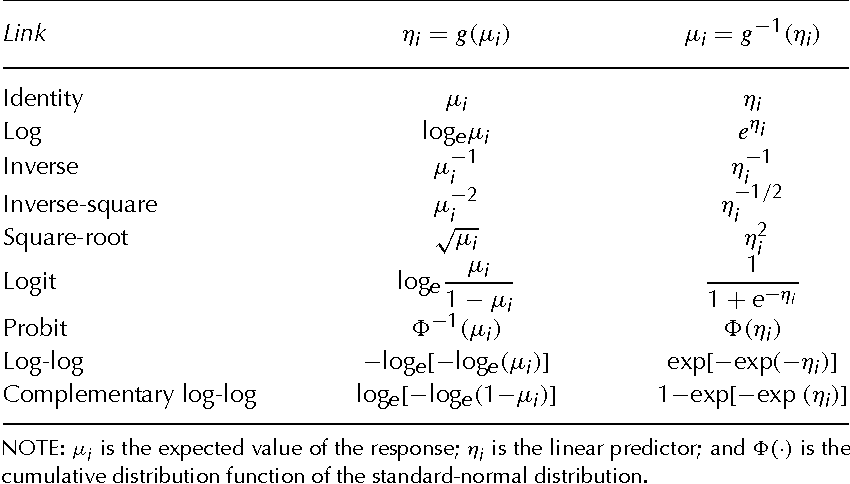
\includegraphics[width=11.81in]{images/2-Table15.1-1} \end{center}

Table 15.1 Generalized Linear Models 15.1 the Structure of Generalized Linear Models

More example on the link functions and their inverses can be found on \href{https://www.sagepub.com/sites/default/files/upm-binaries/21121_Chapter_15.pdf}{page 380}

Example

Normal random component

\begin{itemize}
\item
  Mean Response: \(\mu_i = \theta_i\)
\item
  Canonical Link: \(g( \mu_i) = \mu_i\) (the identity link)
\end{itemize}

Binomial random component

\begin{itemize}
\item
  Mean Response: \(\mu_i = \frac{n_i \exp( \theta)}{1+\exp (\theta_i)}\) and \(\theta(\mu_i) = \log(\frac{p_i }{1-p_i}) = \log (\frac{\mu_i} {n_i - \mu_i})\)
\item
  Canonical link: \(g(\mu_i) = \log(\frac{\mu_i} {n_i - \mu_i})\) (logit link)
\end{itemize}

Poisson random component

\begin{itemize}
\item
  Mean Response: \(\mu_i = \exp(\theta_i)\)
\item
  Canonical Link: \(g(\mu_i) = \log(\mu_i)\)
\end{itemize}

Gamma random component:

\begin{itemize}
\item
  Mean response: \(\mu_i = -\frac{1}{\theta_i}\) and \(\theta(\mu_i) = - \mu_i^{-1}\)
\item
  Canonical Link: \(g(\mu\_i) = - \frac{1}{\mu_i}\)
\end{itemize}

Inverse Gaussian random

\begin{itemize}
\tightlist
\item
  Canonical Link: \(g(\mu_i) = \frac{1}{\mu_i^2}\)
\end{itemize}

\hypertarget{estimation-1}{%
\subsection{Estimation}\label{estimation-1}}

\begin{itemize}
\tightlist
\item
  MLE for parameters of the \textbf{systematic component (}\(\beta\))\\
\item
  Unification of derivation and computation (thanks to the exponential forms)\\
\item
  No unification for estimation of the dispersion parameter (\(\phi\))
\end{itemize}

\hypertarget{estimation-of-beta}{%
\subsubsection{\texorpdfstring{Estimation of \(\beta\)}{Estimation of \textbackslash beta}}\label{estimation-of-beta}}

We have

\[
f(y_i ; \theta_i, \phi) = \exp(\frac{\theta_i y_i - b(\theta_i)}{a(\phi)}+ c(y_i, \phi)) \\
E(Y_i) = \mu_i = b'(\theta) \\
var(Y_i) = b''(\theta)a(\phi) = V(\mu_i)a(\phi) \\
g(\mu_i) = \mathbf{x}_i'\beta = \eta_i
\]

If the log-likelihood for a single observation is \(l_i (\beta,\phi)\). The log-likelihood for all n observations is

\[
\begin{aligned}
l(\beta,\phi) &= \sum_{i=1}^n l_i (\beta,\phi) \\
&= \sum_{i=1}^n (\frac{\theta_i y_i - b(\theta_i)}{a(\phi)}+ c(y_i, \phi))
\end{aligned}
\]

Using MLE to find \(\beta\), we use the chain rule to get the derivatives

\[
\begin{aligned}
\frac{\partial l_i (\beta,\phi)}{\partial \beta_j} &=  \frac{\partial l_i (\beta, \phi)}{\partial \theta_i} \times \frac{\partial \theta_i}{\partial \mu_i} \times \frac{\partial \mu_i}{\partial \eta_i}\times \frac{\partial \eta_i}{\partial \beta_j} \\
&= \sum_{i=1}^{n}(\frac{ y_i - \mu_i}{a(\phi)} \times \frac{1}{V(\mu_i)} \times \frac{\partial \mu_i}{\partial \eta_i} \times x_{ij})
\end{aligned}
\]

If we let

\[
w_i \equiv ((\frac{\partial \eta_i}{\partial \mu_i})^2 V(\mu_i))^{-1}
\]

Then,

\[
\frac{\partial l_i (\beta,\phi)}{\partial \beta_j} = \sum_{i=1}^n (\frac{y_i \mu_i}{a(\phi)} \times w_i \times \frac{\partial \eta_i}{\partial \mu_i} \times x_{ij})
\]

We can also get the second derivatives using the chain rule.

Example:

For the \protect\hyperlink{newton-raphson}{Newton-Raphson} algorithm, we need

\[
- E(\frac{\partial^2 l(\beta,\phi)}{\partial \beta_j \partial \beta_k})
\]

where \((j,k)\)th element of the \textbf{Fisher information matrix} \(\mathbf{I}(\beta)\)

Hence,

\[
- E(\frac{\partial^2 l(\beta,\phi)}{\partial \beta_j \partial \beta_k}) = \sum_{i=1}^n \frac{w_i}{a(\phi)}x_{ij}x_{ik}
\]

for the (j,k)th element

If Bernoulli model with logit link function (which is the canonical link)

\[
b(\theta) = \log(1 + \exp(\theta)) = \log(1 + \exp(\mathbf{x'\beta})) \\
a(\phi) = 1  \\
c(y_i, \phi) = 0 \\
E(Y) = b'(\theta) = \frac{\exp(\theta)}{1 + \exp(\theta)} = \mu = p \\
\eta = g(\mu) = \log(\frac{\mu}{1-\mu}) = \theta = \log(\frac{p}{1-p}) = \mathbf{x'\beta} 
\]

For \(Y_i\), i = 1,.., the log-likelihood is

\[
l_i (\beta, \phi) = \frac{y_i \theta_i - b(\theta_i)}{a(\phi)} + c(y_i, \phi) = y_i \mathbf{x}'_i \beta - \log(1+ \exp(\mathbf{x'\beta}))
\]

Additionally,

\[
V(\mu_i) = \mu_i(1-\mu_i)= p_i (1-p_i) \\
\frac{\partial \mu_i}{\partial \eta_i} = p_i(1-p_i)
\]

Hence,

\[
\begin{aligned}
\frac{\partial l(\beta, \phi)}{\partial \beta_j} &= \sum_{i=1}^n[\frac{y_i - \mu_i}{a(\phi)} \times \frac{1}{V(\mu_i)}\times \frac{\partial \mu_i}{\partial \eta_i} \times x_{ij}] \\
&= \sum_{i=1}^n (y_i - p_i) \times \frac{1}{p_i(1-p_i)} \times p_i(1-p_i) \times x_{ij} \\
&= \sum_{i=1}^n (y_i - p_i) x_{ij} \\
&= \sum_{i=1}^n (y_i - \frac{\exp(\mathbf{x'_i\beta})}{1+ \exp(\mathbf{x'_i\beta})})x_{ij}
\end{aligned}
\]

then

\[
w_i = ((\frac{\partial \eta_i}{\partial \mu_i})^2 V(\mu_i))^{-1} = p_i (1-p_i)
\]

\[
\mathbf{I}_{jk}(\mathbf{\beta}) = \sum_{i=1}^n \frac{w_i}{a(\phi)} x_{ij}x_{ik} = \sum_{i=1}^n p_i (1-p_i)x_{ij}x_{ik}
\]

The \textbf{Fisher-scoring} algorithm for the MLE of \(\mathbf{\beta}\) is

\[
\left(
\begin{array}
{c}
\beta_1 \\
\beta_2 \\
. \\
. \\
. \\
\beta_p \\
\end{array}
\right)^{(m+1)}
=
\left(
\begin{array}
{c}
\beta_1 \\
\beta_2 \\
. \\
. \\
. \\
\beta_p \\
\end{array}
\right)^{(m)} +
\mathbf{I}^{-1}(\mathbf{\beta})
\left(
\begin{array}
{c}
\frac{\partial l (\beta, \phi)}{\partial \beta_1} \\
\frac{\partial l (\beta, \phi)}{\partial \beta_2} \\
. \\
. \\
. \\
\frac{\partial l (\beta, \phi)}{\partial \beta_p} \\
\end{array}
\right)|_{\beta = \beta^{(m)}}
\]

Similar to \protect\hyperlink{newton-raphson}{Newton-Raphson} expect the matrix of second derivatives by the expected value of the second derivative matrix.

In matrix notation,

\[
\begin{aligned}
\frac{\partial l }{\partial \beta} &= \frac{1}{a(\phi)}\mathbf{X'W\Delta(y - \mu)} \\
&= \frac{1}{a(\phi)}\mathbf{F'V^{-1}(y - \mu)} \\
\end{aligned}
\]

\[
\mathbf{I}(\beta) = \frac{1}{a(\phi)}\mathbf{X'WX} = \frac{1}{a(\phi)}\mathbf{F'V^{-1}F} \\
\]

where

\begin{itemize}
\tightlist
\item
  \(\mathbf{X}\) is an n x p matrix of covariates
\item
  \(\mathbf{W}\) is an n x n diagonal matrix with (i,i)th element given by \(w_i\)
\item
  \(\mathbf{\Delta}\) an n x n diagonal matrix with (i,i)th element given by \(\frac{\partial \eta_i}{\partial \mu_i}\)
\item
  \(\mathbf{F} = \mathbf{\frac{\partial \mu}{\partial \beta}}\) an n x p matrix with ith row \(\frac{\partial \mu_i}{\partial \beta} = (\frac{\partial \mu_i}{\partial \eta_i})\mathbf{x}'_i\)
\item
  \(\mathbf{V}\) an n x n diagonal matrix with (i,i)th element given by \(V(\mu_i)\)
\end{itemize}

Setting the derivative of the log-likelihood equal to 0, ML estimating equations are

\[
\mathbf{F'V^{-1}y= F'V^{-1}\mu}
\]

where all components of this equation expect y depends on the parameters \(\beta\)

\textbf{Special Cases}

If one has a canonical link, the estimating equations reduce to

\[
\mathbf{X'y= X'\mu}
\]

If one has an identity link, then

\[
\mathbf{X'V^{-1}y = X'V^{-1}X\hat{\beta}}
\]

which gives the generalized least squares estimator

Generally, we can rewrite the Fisher-scoring algorithm as

\[
\beta^{(m+1)} = \beta^{(m)} + \mathbf{(\hat{F}'\hat{V}^{-1}\hat{F})^{-1}\hat{F}'\hat{V}^{-1}(y- \hat{\mu})}
\]

Since \(\hat{F},\hat{V}, \hat{\mu}\) depend on \(\beta\), we evaluate at \(\beta^{(m)}\)

From starting values \(\beta^{(0)}\), we can iterate until convergence.

Notes:

\begin{itemize}
\tightlist
\item
  if \(a(\phi)\) is a constant or of the form \(m_i \phi\) with known \(m_i\), then \(\phi\) cancels.
\end{itemize}

\hypertarget{estimation-of-phi}{%
\subsubsection{\texorpdfstring{Estimation of \(\phi\)}{Estimation of \textbackslash phi}}\label{estimation-of-phi}}

2 approaches:

\begin{enumerate}
\def\labelenumi{\arabic{enumi}.}
\tightlist
\item
  MLE
\end{enumerate}

\[
\frac{\partial l_i}{\partial \phi} = \frac{(\theta_i y_i - b(\theta_i)a'(\phi))}{a^2(\phi)} + \frac{\partial c(y_i,\phi)}{\partial \phi}
\]

the MLE of \(\phi\) solves

\[
\frac{a^2(\phi)}{a'(\phi)}\sum_{i=1}^n \frac{\partial c(y_i, \phi)}{\partial \phi} = \sum_{i=1}^n(\theta_i y_i - b(\theta_i))
\]

\begin{itemize}
\item
  Situation others than normal error case, expression for \(\frac{\partial c(y,\phi)}{\partial \phi}\) are not simple
\item
  Even for the canonical link and \(a(\phi)\) constant, there is no nice general expression for \(-E(\frac{\partial^2 l}{\partial \phi^2})\), so the unification GLMs provide for estimation of \(\beta\) breaks down for \(\phi\)
\end{itemize}

\begin{enumerate}
\def\labelenumi{\arabic{enumi}.}
\setcounter{enumi}{1}
\item
  Moment Estimation (``Bias Corrected \(\chi^2\)'')

  \begin{itemize}
  \tightlist
  \item
    The MLE is not conventional approach to estimation of \(\phi\) in GLMS.
  \item
    For the exponential family \(var(Y) =V(\mu)a(\phi)\). This implies\\
    \[
    a(\phi) = \frac{var(Y)}{V(\mu)} = \frac{E(Y- \mu)^2}{V(\mu)} \\
    a(\hat{\phi})  = \frac{1}{n-p} \sum_{i=1}^n \frac{(y_i -\hat{\mu}_i)^2}{V(\hat{\mu})}
    \] where p is the dimension of \(\beta\)
  \item
    GLM with canonical link function \(g(.)= (b'(.))^{-1}\)\\
    \[
    g(\mu) = \theta = \eta = \mathbf{x'\beta} \\
    \mu = g^{-1}(\eta)= b'(\eta)
    \]
  \item
    so the method estimator for \(a(\phi)=\phi\) is
  \end{itemize}
\end{enumerate}

\[
\hat{\phi} = \frac{1}{n-p} \sum_{i=1}^n \frac{(y_i - g^{-1}(\hat{\eta}_i))^2}{V(g^{-1}(\hat{\eta}_i))}
\]

\hypertarget{inference-2}{%
\subsection{Inference}\label{inference-2}}

We have

\[
\hat{var}(\beta) = a(\phi)(\mathbf{\hat{F}'\hat{V}\hat{F}})^{-1}
\]

where

\begin{itemize}
\tightlist
\item
  \(\mathbf{V}\) is an n x n diagonal matrix with diagonal elements given by \(V(\mu_i)\)
\item
  \(\mathbf{F}\) is an n x p matrix given by \(\mathbf{F} = \frac{\partial \mu}{\partial \beta}\)
\item
  Both \(\mathbf{V,F}\) are dependent on the mean \(\mu\), and thus \(\beta\). Hence, their estimates (\(\mathbf{\hat{V},\hat{F}}\)) depend on \(\hat{\beta}\).
\end{itemize}

\[
H_0: \mathbf{L\beta = d}
\]

where \(\mathbf{L}\) is a q x p matrix with a \textbf{Wald} test

\[
W = \mathbf{(L \hat{\beta}-d)'(a(\phi)L(\hat{F}'\hat{V}^{-1}\hat{F})L')^{-1}(L \hat{\beta}-d)}
\]

which follows \(\chi_q^2\) distribution (asymptotically), where q is the rank of \(\mathbf{L}\)

In the simple case \(H_0: \beta_j = 0\) gives \(W = \frac{\hat{\beta}^2_j}{\hat{var}(\hat{\beta}_j)} \sim \chi^2_1\) asymptotically

Likelihood ratio test

\[
\Lambda = 2 (l(\hat{\beta}_f)-l(\hat{\beta}_r)) \sim \chi^2_q
\]

where

\begin{itemize}
\tightlist
\item
  q is the number of constraints used to fit the reduced model \(\hat{\beta}_r\), and \(\hat{\beta}_r\) is the fit under the full model.
\end{itemize}

Wald test is easier to implement, but likelihood ratio test is better (especially for small samples).

\hypertarget{deviance}{%
\subsection{Deviance}\label{deviance}}

\protect\hyperlink{deviance}{Deviance} is necessary for goodness of fit, inference and for alternative estimation of the dispersion parameter. We define and consider \protect\hyperlink{deviance}{Deviance} from a likelihood ratio perspective.

\begin{itemize}
\item
  Assume that \(\phi\) is known. Let \(\tilde{\theta}\) denote the full and \(\hat{\theta}\) denote the reduced model MLEs. Then, the likelihood ratio (2 times the difference in log-likelihoods) is \[
  2\sum_{i=1}^{n} \frac{y_i (\tilde{\theta}_i- \hat{\theta}_i)-b(\tilde{\theta}_i) + b(\hat{\theta}_i)}{a_i(\phi)}
  \]
\item
  For exponential families, \(\mu = E(y) = b'(\theta)\), so the natural parameter is a function of \(\mu: \theta = \theta(\mu) = b'^{-1}(\mu)\), and the likelihood ratio turns into\\
  \[
  2 \sum_{i=1}^m \frac{y_i\{\theta(\tilde{\mu}_i - \theta(\hat{\mu}_i)\} - b(\theta(\tilde{\mu}_i)) + b(\theta(\hat{\mu}_i))}{a_i(\phi)}
  \]
\item
  Comparing a fitted model to ``the fullest possible model'', which is the \textbf{saturated model}: \(\tilde{\mu}_i = y_i\), i = 1,..,n.~If \(\tilde{\theta}_i^* = \theta(y_i), \hat{\theta}_i^* = \theta (\hat{\mu})\), the likelihood ratio is\\
  \[
  2 \sum_{i=1}^{n} \frac{y_i (\tilde{\theta}_i^* - \hat{\theta}_i^* + b(\hat{\theta}_i^*))}{a_i(\phi)}
  \]
\item
  \citep{McCullagh_2019} specify \(a(\phi) = \phi\), then the likelihood ratio can be written as\\
  \[
  D^*(\mathbf{y, \hat{\mu}}) = \frac{2}{\phi}\sum_{i=1}^n\{y_i (\tilde{\theta}_i^*- \hat{\theta}_i^*)- b(\tilde{\theta}_i^*) +b(\hat{\theta}_i^*)  \}  
  \] where
\item
  \(D^*(\mathbf{y, \hat{\mu}})\) = \textbf{scaled deviance}
\item
  \(D(\mathbf{y, \hat{\mu}}) = \phi D^*(\mathbf{y, \hat{\mu}})\) = \textbf{deviance}
\end{itemize}

\textbf{Note}:

\begin{itemize}
\item
  in some random component distributions, we can write \(a_i(\phi) = \phi m_i\), where

  \begin{itemize}
  \tightlist
  \item
    \(m_i\) is some known scalar that may change with the observations. THen, the scaled deviance components are divided by \(m_i\):\\
    \[
    D^*(\mathbf{y, \hat{\mu}}) \equiv 2\sum_{i=1}^n\{y_i (\tilde{\theta}_i^*- \hat{\theta}_i^*)- b(\tilde{\theta}_i^*) +b(\hat{\theta}_i^*)\} / (\phi m_i)  
    \]
  \end{itemize}
\item
  \(D^*(\mathbf{y, \hat{\mu}}) = \sum_{i=1}^n d_i\)m where \(d_i\) is the deviance contribution from the ith observation.
\item
  D is used in model selection
\item
  \(D^*\) is used in goodness of fit tests (as it is a likelihood ratio statistic). \[
  D^*(\mathbf{y, \hat{\mu}}) = 2\{l(\mathbf{y,\tilde{\mu}})-l(\mathbf{y,\hat{\mu}})\}
  \]
\item
  \(d_i\) are used to form \textbf{deviance residuals}
\end{itemize}

\textbf{Example}:

\textbf{Normal}

We have

\[
\theta = \mu \\
\phi = \sigma^2 \\
b(\theta) = \frac{1}{2} \theta^2 \\
a(\phi) = \phi
\]

Hence,

\[
\tilde{\theta}_i = y_i \\
\hat{\theta}_i = \hat{\mu}_i = g^{-1}(\hat{\eta}_i) 
\]

And

\[
\begin{aligned}
D &= 2 \sum_{1=1}^n Y^2_i - y_i \hat{\mu}_i - \frac{1}{2}y^2_i + \frac{1}{2} \hat{\mu}_i^2 \\
&= \sum_{i=1}^n y_i^2 - 2y_i \hat{\mu}_i + \hat{\mu}_i^2 \\
&= \sum_{i=1}^n (y_i - \hat{\mu}_i)^2
\end{aligned}
\]

which is the \textbf{residual sum of squares}

\textbf{Poisson}

\[
f(y) = \exp\{y\log(\mu) - \mu - \log(y!)\} \\
\theta = \log(\mu) \\
b(\theta) = \exp(\theta) \\
a(\phi) = 1 \\
\tilde{\theta}_i = \log(y_i) \\
\hat{\theta}_i = \log(\hat{\mu}_i) \\
\hat{\mu}_i = g^{-1}(\hat{\eta}_i)
\]

Then,

\[
\begin{aligned}
D &= 2 \sum_{i = 1}^n y_i \log(y_i) - y_i \log(\hat{\mu}_i) - y_i + \hat{\mu}_i \\
&= 2 \sum_{i = 1}^n y_i \log(\frac{y_i}{\hat{\mu}_i}) - (y_i - \hat{\mu}_i)
\end{aligned}
\]

and

\[
d_i = 2\{y_i \log(\frac{y_i}{\hat{\mu}})- (y_i - \hat{\mu}_i)\}
\]

\hypertarget{analysis-of-deviance}{%
\subsubsection{Analysis of Deviance}\label{analysis-of-deviance}}

The difference in deviance between a reduced and full model, where q is the difference in the number of free parameters, has an asymptotic \(\chi^2_q\). The likelihood ratio test

\[
D^*(\mathbf{y;\hat{\mu}_r}) - D^*(\mathbf{y;\hat{\mu}_f}) = 2\{l(\mathbf{y;\hat{\mu}_f})-l(\mathbf{y;\hat{\mu}_r})\}
\]

this comparison of models is \textbf{Analysis of Deviance}. \protect\hyperlink{generalized-linear-models}{GLM} uses this analysis for model selection.

An estimation of \(\phi\) is

\[
\hat{\phi} = \frac{D(\mathbf{y, \hat{\mu}})}{n - p}
\]

where p = number of parameters fit.

Excessive use of \(\chi^2\) test could be problematic since it is asymptotic \citep{McCullagh_2019}

\hypertarget{deviance-residuals}{%
\subsubsection{Deviance Residuals}\label{deviance-residuals}}

We have \(D = \sum_{i=1}^{n}d_i\). Then, we define \textbf{deviance residuals}

\[
r_{D_i} = \text{sign}(y_i -\hat{\mu}_i)\sqrt{d_i}
\]

Standardized version of deviance residuals is

\[
r_{s,i} = \frac{y_i -\hat{\mu}}{\hat{\sigma}(1-h_{ii})^{1/2}}
\]

Let \(\mathbf{H^{GLM} = W^{1/2}X(X'WX)^{-1}X'W^{-1/2}}\), where \(\mathbf{W}\) is an n x n diagonal matrix with (i,i)th element given by \(w_i\) (see \protect\hyperlink{estimation-of-beta}{Estimation of \(\beta\)}). Then Standardized deviance residuals is equivalently

\[
r_{s, D_i} = \frac{r_{D_i}}{\{\hat{\phi}(1-h_{ii}^{glm}\}^{1/2}}
\]

where \(h_{ii}^{glm}\) is the ith diagonal of \(\mathbf{H}^{GLM}\)

\hypertarget{pearson-chi-square-residuals}{%
\subsubsection{Pearson Chi-square Residuals}\label{pearson-chi-square-residuals}}

Another \(\chi^2\) statistic is \textbf{Pearson} \(\chi^2\) statistics: (assume \(m_i = 1\))

\[
X^2 = \sum_{i=1}^{n} \frac{(y_i - \hat{\mu}_i)^2}{V(\hat{\mu}_i)}
\]

where \(\hat{\mu}_i\) is the fitted mean response fo the model of interest.

The \textbf{Scaled Pearson} \(\chi^2\) statistic is given by \(\frac{X^2}{\phi} \sim \chi^2_{n-p}\) where p is the number of parameters estimated. Hence, the \textbf{Pearson} \(\chi^2\) residuals are

\[
X^2_i = \frac{(y_i - \hat{\mu}_i)^2}{V(\hat{\mu}_i)}
\]

If we have the following assumptions:

\begin{itemize}
\tightlist
\item
  Independent samples\\
\item
  No over-dispersion: If \(\phi = 1\), \(\frac{D(\mathbf{y;\hat{\mu}})}{n-p}\) and \(\frac{X^2}{n-p}\) have a value substantially larger 1 indicates \textbf{improperly specified model} or \textbf{overdispersion}\\
\item
  Multiple groups
\end{itemize}

then \(\frac{X^2}{\phi}\) and \(D^*(\mathbf{y; \hat{\mu}})\) both follow \(\chi^2_{n-p}\)

\hypertarget{diagnostic-plots}{%
\subsection{Diagnostic Plots}\label{diagnostic-plots}}

\begin{itemize}
\item
  Standardized residual Plots:

  \begin{itemize}
  \tightlist
  \item
    plot(\(r_{s, D_i}\), \(\hat{\mu}_i\)) or plot(\(r_{s, D_i}\), \(T(\hat{\mu}_i)\)) where \(T(\hat{\mu}_i)\) is transformation(\(\hat{\mu}_i\)) called \textbf{constant information scale}:\\
  \item
    plot(\(r_{s, D_i}\), \(\hat{\eta}_i\))
  \end{itemize}
\end{itemize}

\begin{longtable}[]{@{}cc@{}}
\toprule
Random Component & \(T(\hat{\mu}_i)\)\tabularnewline
\midrule
\endhead
Normal & \(\hat{\mu}\)\tabularnewline
Poisson & \(2\sqrt{\mu}\)\tabularnewline
Binomial & \(2 \sin^{-1}(\sqrt{\hat{\mu}})\)\tabularnewline
Gamma & \(2 \log(\hat{\mu})\)\tabularnewline
Inverse Gaussian & \(-2\hat{\mu}^{-1/2}\)\tabularnewline
\bottomrule
\end{longtable}

\begin{itemize}
\item
  If we see:

  \begin{itemize}
  \tightlist
  \item
    Trend, it means we might have a wrong link function, or choice of scale\\
  \item
    Systematic change in range of residuals with a change in \(T(\hat{\mu})\) (incorrect random component) (systematic \(\neq\) random)\\
  \end{itemize}
\item
  plot(\(|r_{D_i}|,\hat{\mu}_i\)) to check \textbf{Variance Function}.
\end{itemize}

\hypertarget{goodness-of-fit}{%
\subsection{Goodness of Fit}\label{goodness-of-fit}}

To assess goodness of fit, we can use

\begin{itemize}
\tightlist
\item
  \protect\hyperlink{deviance}{Deviance}\\
\item
  \protect\hyperlink{pearson-chi-square-residuals}{Pearson Chi-square Residuals}
\end{itemize}

In nested model, we could use likelihood-based information measures:

\[
AIC = -2l(\mathbf{\hat{\mu}}) + 2p \\
AICC = -2l(\mathbf{\hat{\mu}}) + 2p(\frac{n}{n-p-1}) \\
BIC = 2l(\hat{\mu}) + p \log(n)
\]

where

\begin{itemize}
\tightlist
\item
  \(l(\hat{\mu})\) is the log-likelihood evaluated at the parameter estimates
\item
  p is the number of parameters
\item
  n is the number of observations.
\end{itemize}

Note: you have to use the same data with the same model (i.e., same link function, same random underlying random distribution). but you can have different number of parameters.

Even though statisticians try to come up with measures that are similar to \(R^2\), in practice, it is not so appropriate. For example, they comapre the log-likelihood of the fitted model against the that of a model with jsut the intercept:

\[
R^2_p = 1 - \frac{l(\hat{\mu})}{l(\hat{\mu}_0)}
\]

For certain specific random components such as binary response model, we have **rescaled generalized \(R^2\):

\[
\bar{R}^2 = \frac{R^2_*}{\max(R^2_*)} = \frac{1-\exp\{-\frac{2}{n}(l(\hat{\mu}) - l(\hat{\mu}_0) \}}{1 - \exp\{\frac{2}{n}l(\hat{\mu}_0)\}}
\]

\hypertarget{over-dispersion}{%
\subsection{Over-Dispersion}\label{over-dispersion}}

\begin{longtable}[]{@{}lll@{}}
\toprule
Random Components & \(var(Y)\) & \(V(\mu)\)\tabularnewline
\midrule
\endhead
Binomial & \(var(Y) = n \mu (1- \mu)\) & \(V(\mu) = \phi n \mu(1- \mu)\) where \(m_i =n\)\tabularnewline
Poisson & \(var(Y) = \mu\) & \(V(\mu) = \phi \mu\)\tabularnewline
\bottomrule
\end{longtable}

In both cases \(\phi = 1\). Recall \(b''(\theta)= V(\mu)\) check \protect\hyperlink{estimation-of-phi}{Estimation of \(\phi\)}.

If we find

\begin{itemize}
\tightlist
\item
  \(\phi >1\): over-dispersion (i.e., too much variation for an independent binomial or Poisson distribution).
\item
  \(\phi<1\): under-dispersion (i.e., too little variation for an independent binomial or Poisson distribution).
\end{itemize}

If we have either over or under-dispersion, it means we might have unspecified random component, we could

\begin{itemize}
\tightlist
\item
  Select a different random component distribution that can accommodate over or under-dispersion (e.g., negative binomial, Conway-Maxwell Poisson)
\item
  use \protect\hyperlink{nonlinear-and-generalized-linear-mixed-models}{Generalized Linear Mixed Models} to handle random effects in generalized linear models.
\end{itemize}

\hypertarget{linear-mixed-models}{%
\chapter{Linear Mixed Models}\label{linear-mixed-models}}

\hypertarget{dependent-data}{%
\section{Dependent Data}\label{dependent-data}}

Forms of dependent data:

\begin{itemize}
\tightlist
\item
  Multivariate measurements on different individuals: (e.g., a person's blood pressure, fat, etc are correlated)
\item
  Clustered measurements: (e.g., blood pressure measurements of people in the same family can be correlated).
\item
  Repeated measurements: (e.g., measurement of cholesterol over time can be correlated) ``If data are collected repeatedly on experimental material to which treatments were applied initially, the data is a repeated measure.'' \citep{Schabenberger_2001}
\item
  Longitudinal data: (e.g., individual's cholesterol tracked over time are correlated): ``data collected repeatedly over time in an observational study are termed longitudinal.'' \citep{Schabenberger_2001}
\item
  Spatial data: (e.g., measurement of individuals living in the same neighborhood are correlated)
\end{itemize}

Hence, we like to account for these correlations.

\textbf{Linear Mixed Model} (LMM), also known as \textbf{Mixed Linear Model} has 2 components:

\begin{itemize}
\item
  \textbf{Fixed effect} (e.g, gender, age, diet, time)
\item
  \textbf{Random effects} representing individual variation or auto correlation/spatial effects that imply \textbf{dependent (correlated) errors}
\end{itemize}

Review \protect\hyperlink{two-way-mixed-effects-anova}{Two-Way Mixed Effects ANOVA}

We choose to model the random subject-specific effect instead of including dummy subject covariates in our model because:

\begin{itemize}
\tightlist
\item
  reduction in the number of parameters to estimate
\item
  when you do inference, it would make more sense that you can infer from a population (i.e., random effect).
\end{itemize}

\textbf{LLM Motivation}

In a repeated measurements analysis where \(Y_{ij}\) is the response for the i-th individual measured at the j-th time,

\(i =1,…,N\) ; \(j = 1,…,n_i\)

\[
\mathbf{Y}_i = 
\left(
\begin{array}
{c}
Y_{i1} \\
. \\
.\\
.\\
Y_{in_i}
\end{array}
\right)
\]

is all measurements for subject i.

\underline{\emph{Stage 1: (Regression Model)}} how the response changes over time for the ith subject

\[
\mathbf{Y_i = Z_i \beta_i + \epsilon_i}
\]

where

\begin{itemize}
\tightlist
\item
  \(Z_i\) is an \(n_i \times q\) matrix of known covariates
\item
  \(\beta_i\) is an unknown q x 1 vector of subjective -specific coefficients (regression coefficients different for each subject)
\item
  \(\epsilon_i\) are the random errors (typically \(\sim N(0, \sigma^2 I)\))
\end{itemize}

We notice that there are two many \(\beta\) to estimate here. Hence, this is the motivation for the second stage

\underline{\emph{Stage 2: (Parameter Model)}}

\[
\mathbf{\beta_i = K_i \beta + b_i}
\]

where

\begin{itemize}
\tightlist
\item
  \(K_i\) is a q x p matrix of known covariates
\item
  \(\beta\) is a p x 1 vector of unknown parameter
\item
  \(\mathbf{b}_i\) are independent \(N(0,D)\) random variables
\end{itemize}

This model explain the observed variability between subjects with respect to the subject-specific regression coefficients, \(\beta_i\). We model our different coefficient (\(\beta_i\)) with respect to \(\beta\).

Example:

Stage 1:

\[
Y_{ij} = \beta_{1i} + \beta_{2i}t_{ij} + \epsilon_{ij}
\]

where

\begin{itemize}
\tightlist
\item
  \(j = 1,..,n_i\)
\end{itemize}

In the matrix notation,

\[
\mathbf{Y_i} = 
\left(
\begin{array}
{c}
Y_{i1} \\
.\\
Y_{in_i}
\end{array}
\right)
\]

\[
\mathbf{Z}_i = 
\left(
\begin{array}
{cc}
1 & t_{i1} \\
. & . \\
1 & t_{in_i} 
\end{array}
\right)
\]

\[
\beta_i =
\left(
\begin{array}
{c}
\beta_{1i} \\
\beta_{2i}
\end{array}
\right)
\]

\[
\epsilon_i = 
\left(
\begin{array}
{c}
\epsilon_{i1} \\
. \\
\epsilon_{in_i}
\end{array}
\right)
\]

Thus,

\[
\mathbf{Y_i = Z_i \beta_i + \epsilon_i}
\]

Stage 2:

\[
\beta_{1i} = \beta_0 + b_{1i} \\
\beta_{2i} = \beta_1 L_i + \beta_2 H_i + \beta_3 C_i + b_{2i}
\]

where \(L_i, H_i, C_i\) are indicator variables defined to 1 as the subject falls into different categories.

Subject specific intercepts do not depend upon treatment, with \(\beta_0\) (the average response at the start of treatment), and \(\beta_1 , \beta_2, \beta_3\) (the average time effects for each of three treatment groups).

\[
\mathbf{K}_i = \left(
\begin{array}
{cccc}
1 & 0 & 0 & 0 \\
0 & L_i & H_i & C_i 
\end{array}
\right) \\ \beta = (\beta_0 , \beta_1, \beta_2, \beta_3)' \\ 
\mathbf{b}_i = 
\left(
\begin{array}
{c}
b_{1i} \\
b_{2i} \\
\end{array}
\right) \\ 
\beta_i = \mathbf{K_i \beta + b_i}
\]

To get \(\hat{\beta}\), we can fit the model sequentially:

\begin{enumerate}
\def\labelenumi{\arabic{enumi}.}
\tightlist
\item
  Estimate \(\hat{\beta_i}\) in the first stage
\item
  Estimate \(\hat{\beta}\) in the second stage by replacing \(\beta_i\) with \(\hat{\beta}_i\)
\end{enumerate}

However, problems arise from this method:

\begin{itemize}
\tightlist
\item
  information is lost by summarizing the vector \(\mathbf{Y}_i\) solely by \(\hat{\beta}_i\)
\item
  we need to account for variability when replacing \(\beta_i\) with its estimate
\item
  different subjects might have different number of observations.
\end{itemize}

To address these problems, we can use \textbf{Linear Mixed Model \citep{Laird_1982}}

Substituting stage 2 into stage 1:

\[
\mathbf{Y}_i = \mathbf{Z}_i \mathbf{K}_i \beta + \mathbf{Z}_i \mathbf{b}_i + \mathbf{\epsilon}_i
\]

Let \(\mathbf{X}_i = \mathbf{Z}_i \mathbf{K}_i\) be an \(n_i \times p\) matrix . Then, the LMM is

\[
\mathbf{Y}_i = \mathbf{X}_i \beta + \mathbf{Z}_i \mathbf{b}_i + \mathbf{\epsilon}_i
\]

where

\begin{itemize}
\tightlist
\item
  \(i = 1,..,N\)
\item
  \(\beta\) are the fixed effects, which are common to all subjects
\item
  \(\mathbf{b}_i\) are the subject specific random effects. \(\mathbf{b}_i \sim N_q (\mathbf{0,D})\)
\item
  \(\mathbf{\epsilon}_i \sim N_{n_i}(\mathbf{0,\Sigma_i})\)
\item
  \(\mathbf{b}_i\) and \(\epsilon_i\) are independent
\item
  \(\mathbf{Z}_{i(n_i \times q})\) and \(\mathbf{X}_{i(n_i \times p})\) are matrices of known covariates.
\end{itemize}

Equivalently, in the hierarchical form, we call \textbf{conditional} or \textbf{hierarchical} formulation of the linear mixed model

\[
\mathbf{Y}_i | \mathbf{b}_i \sim N(\mathbf{X}_i \beta+ \mathbf{Z}_i \mathbf{b}_i, \mathbf{\Sigma}_i) \\
\mathbf{b}_i \sim N(\mathbf{0,D})
\]

for \(i = 1,..,N\). denote the respective functions by \(f(\mathbf{Y}_i |\mathbf{b}_i)\) and \(f(\mathbf{b}_i)\)

In general,

\[
f(A,B) = f(A|B)f(B) \\
f(A) = \int f(A,B)dB = \int f(A|B) f(B) dB
\]

In the LMM, the marginal density of \(\mathbf{Y}_i\) is

\[
f(\mathbf{Y}_i) = \int f(\mathbf{Y}_i | \mathbf{b}_i) f(\mathbf{b}_i) d\mathbf{b}_i
\]

which can be shown

\[
\mathbf{Y}_i \sim N(\mathbf{X_i \beta, Z_i DZ'_i + \Sigma_i})
\]

This is the \textbf{marginal} formulation of the linear mixed model

Notes:

We no longer have \(Z_i b_i\) in the mean, but add error in the variance (marginal dependence in Y). kinda of averaging out the common effect. Technically, we shouldn't call it averaging the error b (adding it to the variance covariance matrix), it should be called adding random effect

Continue with our example

\[
Y_{ij} = (\beta_0 + b_{1i}) + (\beta_1L_i + \beta_2 H_i + \beta_3 C_i + b_{2i})t_{ij} + \epsilon_{ij}
\]

for each treatment group

\[
Y_{ik}= 
\begin{cases}
\beta_0 + b_{1i} + (\beta_1 + \ b_{2i})t_{ij} + \epsilon_{ij} & L \\
\beta_0 + b_{1i} + (\beta_2 + \ b_{2i})t_{ij} + \epsilon_{ij} & H\\
\beta_0 + b_{1i} + (\beta_3 + \ b_{2i})t_{ij} + \epsilon_{ij} & C
\end{cases}
\]

\begin{itemize}
\tightlist
\item
  Intercepts and slopes are all subject specific
\item
  Different treatment groups have different slops, but the same intercept.
\end{itemize}

\textbf{In the hierarchical model form}

\[
\mathbf{Y}_i | \mathbf{b}_i \sim N(\mathbf{X}_i \beta + \mathbf{Z}_i \mathbf{b}_i, \mathbf{\Sigma}_i)\\
\mathbf{b}_i \sim N(\mathbf{0,D})
\]

X will be in the form of

\[
\mathbf{X}_i = \mathbf{Z}_i \mathbf{K}_i \\
= 
\left[
\begin{array}
{cc}
1 & t_{i1} \\
1 & t_{i2} \\
. & . \\
1 & t_{in_i}
\end{array}
\right]
\times
\left[
\begin{array}
{cccc}
1 & 0 & 0 & 0 \\
0 & L_i & H_i & C_i \\
\end{array}
\right] \\
=
\left[ 
\begin{array}
{cccc}
1 & t_{i1}L_i & t_{i1}H_i & T_{i1}C_i \\
1 & t_{i2}L_i & t_{i2}H_i & T_{i2}C_i \\
. &. &. &. \\
1 & t_{in_i}L_i & t_{in_i}H_i & T_{in_i}C_i \\
\end{array}
\right]
\]

\[
\beta = (\beta_0, \beta_1, \beta_2, \beta_3)' \\
\mathbf{b}_i = 
\left(
\begin{array}
{c}
b_{1i} \\
b_{2i}
\end{array}
\right)
,
D = 
\left(
\begin{array}
{cc}
d_{11} & d_{12}\\
d_{12} & d_{22}
\end{array}
\right)
\]

Assuming \(\mathbf{\Sigma}_i = \sigma^2 \mathbf{I}_{n_i}\), which is called \textbf{conditional independence}, meaning the response on subject i are independent conditional on \(\mathbf{b}_i\) and \(\beta\)

\textbf{In the marginal model form}

\[
Y_{ij} = \beta_0 + \beta_1 L_i t_{ij} + \beta_2 H_i t_{ij} + \beta_3 C_i t_{ij} + \eta_{ij}
\]

where \(\eta_i \sim N(\mathbf{0},\mathbf{Z}_i\mathbf{DZ}_i'+ \mathbf{\Sigma}_i)\)

Equivalently,

\[
\mathbf{Y_i \sim N(X_i \beta, Z_i DZ_i' + \Sigma_i})
\]

In this case that \(n_i = 2\)

\[
\mathbf{Z_iDZ_i'} = 
\left(
\begin{array}
{cc}
1 & t_{i1} \\
1 & t_{i2} 
\end{array}
\right)
\left(
\begin{array}
{cc}
d_{11} & d_{12} \\
d_{12} & d_{22} 
\end{array}
\right)
\left(
\begin{array}
{cc}
1 & 1 \\
t_{i1} & t_{i2} 
\end{array}
\right) \\
=
\left(
\begin{array}
{cc}
d_{11} + 2d_{12}t_{i1} + d_{22}t_{i1}^2 & d_{11} + d_{12}(t_{i1} + t_{i2}) + d_{22}t_{i1}t_{i2} \\
d_{11} + d_{12}(t_{i1} + t_{i2}) + d_{22} t_{i1} t_{i2} & d_{11} + 2d_{12}t_{i2} + d_{22}t_{i2}^2  
\end{array}
\right)
\]

\[
var(Y_{i1}) = d_{11} + 2d_{12}t_{i1} + d_{22} t_{i1}^2 + \sigma^2
\]

On top of correlation in the errors, the marginal implies that the variance function of the response is quadratic over time, with positive curvature \(d_{22}\)

\hypertarget{random-intercepts-model}{%
\subsection{Random-Intercepts Model}\label{random-intercepts-model}}

If we remove the random slopes,

\begin{itemize}
\tightlist
\item
  the assumption is that all variability in subject-specific slopes can be attributed to treatment differences
\item
  the model is random-intercepts model. This has subject specific intercepts, but the same slopes within each treatment group.
\end{itemize}

\[
\mathbf{Y}_i | b_i \sim N(\mathbf{X}_i \beta + 1 b_i , \Sigma_i) \\
b_i \sim N(0,d_{11})
\]

The marginal model is then (\(\mathbf{\Sigma}_i = \sigma^2 \mathbf{I}\))

\[
\mathbf{Y}_i \sim N(\mathbf{X}_i \beta, 11'd_{11} + \sigma^2 \mathbf{I})
\]

The marginal covariance matrix is

\[
cov(\mathbf{Y}_i)  = 11'd_{11} + \sigma^2I \\
=
\left(
\begin{array}
{cccc}
d_{11}+ \sigma^2 & d_{11} & ... & d_{11} \\
d_{11} & d_{11} + \sigma^2 & d_{11} & ... \\
. & . & . & . \\
d_{11} & ... & ... & d_{11} + \sigma^2
\end{array}
\right)
\]

the associated correlation matrix is

\[
corr(\mathbf{Y}_i) = 
\left(
\begin{array}
{cccc}
1 & \rho & ... & \rho \\
\rho & 1 & \rho & ... \\
. & . & . & . \\
\rho & ... & ... & 1 \\
\end{array}
\right)
\]

where \(\rho \equiv \frac{d_{11}}{d_{11} + \sigma^2}\)

Thu, we have

\begin{itemize}
\tightlist
\item
  constant variance over time
\item
  equal, positive correlation between any two measurements from the same subject
\item
  a covariance structure that is called \textbf{compound symmetry}, and \(\rho\) is called the \textbf{intra-class correlation}
\item
  that when \(\rho\) is large, the \textbf{inter-subject variability} (\(d_{11}\)) is large relative to the intra-subject variability (\(\sigma^2\))
\end{itemize}

\hypertarget{covariance-models}{%
\subsection{Covariance Models}\label{covariance-models}}

If the conditional independence assumption, (\(\mathbf{\Sigma_i= \sigma^2 I_{n_i}}\)). Consider, \(\epsilon_i = \epsilon_{(1)i} + \epsilon_{(2)i}\), where

\begin{itemize}
\tightlist
\item
  \(\epsilon_{(1)i}\) is a ``serial correlation'' component. That is, part of the individual's profile is a response to time-varying stochastic processes.
\item
  \(\epsilon_{(2)i}\) is the measurement error component, and is independent of \(\epsilon_{(1)i}\)
\end{itemize}

Then

\[
\mathbf{Y_i = X_i \beta + Z_i b_i + \epsilon_{(1)i} + \epsilon_{(2)i}}
\]

where

\begin{itemize}
\item
  \(\mathbf{b_i} \sim N(\mathbf{0,D})\)
\item
  \(\epsilon_{(2)i} \sim N(\mathbf{0,\sigma^2 I_{n_i}})\)
\item
  \(\epsilon_{(1)i} \sim N(\mathbf{0,\tau^2H_i})\)
\item
  \(\mathbf{b}_i\) and \(\epsilon_i\) are mutually independent
\end{itemize}

To model the structure of the \(n_i \times n_i\) correlation (or covariance ) matrix \(\mathbf{H}_i\). Let the (j,k)th element of \(\mathbf{H}_i\) be \(h_{ijk}= g(t_{ij}t_{ik})\). that is a function of the times \(t_{ij}\) and \(t_{ik}\) , which is assumed to be some function of the "distance' between the times.

\[
h_{ijk} = g(|t_{ij}-t_{ik}|)
\]

for some decreasing function \(g(.)\) with \(g(0)=1\) (for correlation matrices).

Examples of this type of function:

\begin{itemize}
\tightlist
\item
  Exponential function: \(g(|t_{ij}-t_{ik}|) = \exp(-\phi|t_{ij} - t_{ik}|)\)
\item
  Gaussian function: \(g(|t_{ij} - t_{ik}|) = \exp(-\phi(t_{ij} - t_{ik})^2)\)
\end{itemize}

Similar structures could also be used for \(\mathbf{D}\) matrix (of \(\mathbf{b}\))

Example: Autoregressive Covariance Structure

A first order Autoregressive Model (AR(1)) has the form

\[
\alpha_t = \phi \alpha_{t-1} + \eta_t
\]

where \(\eta_t \sim iid N (0,\sigma^2_\eta)\)

Then, the covariance between two observations is

\[
cov(\alpha_t, \alpha_{t+h}) = \frac{\sigma^2_\eta \phi^{|h|}}{1- \phi^2}
\]

for \(h = 0, \pm 1, \pm 2, ...; |\phi|<1\)

Hence,

\[
corr(\alpha_t, \alpha_{t+h}) = \phi^{|h|}
\]

If we let \(\alpha_T = (\alpha_1,...\alpha_T)'\), then

\[
corr(\alpha_T) = 
\left[
\begin{array}
{ccccc}
1 & \phi^1 & \phi^2 & ... & \phi^2 \\
\phi^1 & 1 & \phi^1 & ... & \phi^{T-1} \\
\phi^2 & \phi^1 & 1 & ... & \phi^{T-2} \\
. & . & . & . &. \\
\phi^T & \phi^{T-1} & \phi^{T-2} & ... & 1
\end{array}
\right]
\]

Notes:

\begin{itemize}
\tightlist
\item
  The correlation decreases as time lag increases
\item
  This matrix structure is known as a \textbf{Toeplitz} structure
\item
  More complicated covariance structures are possible, which is critical component of spatial random effects models and time series models.
\item
  Often, we don't need both random effects \(\mathbf{b}\) and \(\epsilon_{(1)i}\)
\end{itemize}

More in the \protect\hyperlink{time-series-1}{Time Series} section

\hypertarget{estimation-2}{%
\section{Estimation}\label{estimation-2}}

\[
\mathbf{Y}_i = \mathbf{X}_i \beta + \mathbf{Z}_i \mathbf{b}_i + \epsilon_i
\]

where \(\beta, \mathbf{b}_i, \mathbf{D}, \mathbf{\Sigma}_i\) we must obtain estimation from the data

\begin{itemize}
\tightlist
\item
  \(\mathbf{\beta}, \mathbf{D}, \mathbf{\Sigma}_i\) are unknown, but fixed, parameters, and must be estimated from the data
\item
  \(\mathbf{b}_i\) is a random variable. Thus, we can't estimate these values, but we can predict them. (i.e., you can't estimate a random thing).
\end{itemize}

If we have

\begin{itemize}
\tightlist
\item
  \(\hat{\beta}\) as an estimator of \(\beta\)
\item
  \(\mathbf{b}_i\) as a predictor of \(\mathbf{b}_i\)
\end{itemize}

Then,

\begin{itemize}
\tightlist
\item
  The population average estimate of \(\mathbf{Y}_i\) is \(\hat{\mathbf{Y}_i} = \mathbf{X}_i \hat{\beta}\)
\item
  The subject-specific prediction is \(\hat{\mathbf{Y}_i} = \mathbf{X}_i \hat{\beta} + \mathbf{Z}_i \hat{b}_i\)
\end{itemize}

According to \citep{Henderson_1950}, estimating equations known as the mixed model equations:

\[
\left[
\begin{array}
{c}
\hat{\beta} \\
\hat{\mathbf{b}}
\end{array}
\right]
=
\left[
\begin{array}
{cc}
\mathbf{X'\Sigma^{-1}X} & \mathbf{X'\Sigma^{-1}Z} \\
\mathbf{Z'\Sigma^{-1}X} & \mathbf{Z'\Sigma^{-1}Z +B^{-1}}
\end{array}
\right]
\left[
\begin{array}
{cc}
\mathbf{X'\Sigma^{-1}Y} \\
\mathbf{Z'\Sigma^{-1}Y}
\end{array}
\right]
\]

where

\[
\mathbf{Y}
=
\left[
\begin{array}
{c}
\mathbf{y}_1 \\
. \\
\mathbf{y}_N
\end{array}
\right] ;
\mathbf{X}
=
\left[
\begin{array}
{c}
\mathbf{X}_1 \\
. \\
\mathbf{X}_N
\end{array}
\right];
\mathbf{b} = 
\left[
\begin{array}
{c}
\mathbf{b}_1 \\
. \\
\mathbf{b}_N
\end{array}
\right] ;
\epsilon = 
\left[
\begin{array}
{c}
\epsilon_1 \\
. \\
\epsilon_N
\end{array}
\right]
\\
cov(\epsilon) = \mathbf{\Sigma},
\mathbf{Z} = 
\left[
\begin{array}
{cccc}
\mathbf{Z}_1 & 0 &  ... & 0 \\
0 & \mathbf{Z}_2 & ... & 0 \\
. & . & . & . \\
0 & 0 & ... & \mathbf{Z}_n
\end{array}
\right],
\mathbf{B} =
\left[
\begin{array}
{cccc}
\mathbf{D} & 0 & ... & 0 \\
0 & \mathbf{D} & ... & 0 \\
. & . & . & . \\
0 & 0 & ... & \mathbf{D}
\end{array}
\right]
\]

The model has the form

\[
\mathbf{Y = X \beta + Z b + \epsilon} \\
\mathbf{Y} \sim N(\mathbf{X \beta, ZBZ' + \Sigma})
\]

If \(\mathbf{V = ZBZ' + \Sigma}\), then the solutions to the estimating equations can be

\[
\hat{\beta} = \mathbf{(X'V^{-1}X)^{-1}X'V^{-1}Y} \\
\hat{\mathbf{b}} = \mathbf{BZ'V^{-1}(Y-X\hat{\beta}})
\]

The estimate \(\hat{\beta}\) is a generalized least squares estimate.

The predictor, \(\hat{\mathbf{b}}\) is the best linear unbiased predictor (BLUP), for \(\mathbf{b}\)

\[
E(\hat{\beta}) = \beta \\
var(\hat{\beta}) = (\mathbf{X'V^{-1}X})^{-1} \\
E(\hat{\mathbf{b}}) = 0 \\
var(\mathbf{\hat{b}-b}) = \mathbf{B-BZ'V^{-1}ZB + BZ'V^{-1}X(X'V^{-1}X)^{-1}X'V^{-1}B}
\]

The variance here is the variance of the prediction error (mean squared prediction error, MSPE), which is more meaningful than \(var(\hat{\mathbf{b}})\), since MSPE accounts for both variance and bias in the prediction.

To derive the mixed model equations, consider

\[
\mathbf{\epsilon = Y - X\beta - Zb}
\]

Let \(T = \sum_{i=1}^N n_i\) be the total number of observations (i.e., the length of \(\mathbf{Y},\epsilon\)) and \(Nq\) the length of \(\mathbf{b}\). The joint distribution of \(\mathbf{b, \epsilon}\) is

\[
f(\mathbf{b,\epsilon})= \frac{1}{(2\pi)^{(T+ Nq)/2}}
\left|
\begin{array}
{cc}
\mathbf{B} & 0 \\
0 & \mathbf{\Sigma}
\end{array}
\right| ^{-1/2}
\exp
\left(
-\frac{1}{2}
\left[
\begin{array}
{c}
\mathbf{b} \\
\mathbf{Y - X \beta - Zb}
\end{array}
\right]'
\left[
\begin{array}
{cc}
\mathbf{B} & 0 \\
0 & \mathbf{\Sigma}
\end{array}
\right]^{-1}
\left[
\begin{array}
{c}
\mathbf{b} \\
\mathbf{Y - X \beta - Zb}
\end{array}
\right]
\right)
\]

Maximization of \(f(\mathbf{b},\epsilon)\) with respect to \(\mathbf{b}\) and \(\beta\) requires minimization of

\[
Q = 
\left[
\begin{array}
{c}
\mathbf{b} \\
\mathbf{Y - X \beta - Zb}
\end{array}
\right]'
\left[
\begin{array}
{cc}
\mathbf{B} & 0 \\
0 & \mathbf{\Sigma}
\end{array}
\right]^{-1}
\left[
\begin{array}
{c}
\mathbf{b} \\
\mathbf{Y - X \beta - Zb}
\end{array}
\right] \\
= \mathbf{b'B^{-1}b+(Y-X \beta-Zb)'\Sigma^{-1}(Y-X \beta-Zb)}
\]

Setting the derivatives of Q with respect to \(\mathbf{b}\) and \(\mathbf{\beta}\) to zero leads to the system of equations:

\[
\begin{aligned}
\mathbf{X'\Sigma^{-1}X\beta + X'\Sigma^{-1}Zb} &= \mathbf{X'\Sigma^{-1}Y}\\
\mathbf{(Z'\Sigma^{-1}Z + B^{-1})b + Z'\Sigma^{-1}X\beta} &= \mathbf{Z'\Sigma^{-1}Y}
\end{aligned}
\]

Rearranging

\[
\left[
\begin{array}
{cc}
\mathbf{X'\Sigma^{-1}X} & \mathbf{X'\Sigma^{-1}Z} \\
\mathbf{Z'\Sigma^{-1}X} & \mathbf{Z'\Sigma^{-1}Z + B^{-1}}
\end{array}
\right]
\left[
\begin{array}
{c}
\beta \\
\mathbf{b}
\end{array}
\right]
= 
\left[
\begin{array}
{c}
\mathbf{X'\Sigma^{-1}Y} \\
\mathbf{Z'\Sigma^{-1}Y}
\end{array}
\right]
\]

Thus, the solution to the mixed model equations give:

\[
\left[
\begin{array}
{c}
\hat{\beta} \\
\hat{\mathbf{b}}
\end{array}
\right]
= 
\left[
\begin{array}
{cc}
\mathbf{X'\Sigma^{-1}X} & \mathbf{X'\Sigma^{-1}Z} \\
\mathbf{Z'\Sigma^{-1}X} & \mathbf{Z'\Sigma^{-1}Z + B^{-1}}
\end{array}
\right]
\left[
\begin{array}
{c}
\mathbf{X'\Sigma^{-1}Y} \\
\mathbf{Z'\Sigma^{-1}Y}
\end{array}
\right]
\]

Equivalently,

Bayes' theorem

\[
f(\mathbf{b}| \mathbf{Y}) = \frac{f(\mathbf{Y}|\mathbf{b})f(\mathbf{b})}{\int f(\mathbf{Y}|\mathbf{b})f(\mathbf{b}) d\mathbf{b}}
\]

where

\begin{itemize}
\tightlist
\item
  \(f(\mathbf{Y}|\mathbf{b})\) is the ``likelihood''
\item
  \(f(\mathbf{b})\) is the prior
\item
  the denominator is the ``normalizing constant''
\item
  \(f(\mathbf{b}|\mathbf{Y})\) is the posterior distribution
\end{itemize}

In this case

\[
\mathbf{Y} | \mathbf{b} \sim N(\mathbf{X\beta+Zb,\Sigma}) \\
\mathbf{b} \sim N(\mathbf{0,B})
\]

The posterior distribution has the form

\[
\mathbf{b}|\mathbf{Y} \sim N(\mathbf{BZ'V^{-1}(Y-X\beta),(Z'\Sigma^{-1}Z + B^{-1})^{-1}})
\]

Hence, the best predictor (based on squared error loss)

\[
E(\mathbf{b}|\mathbf{Y}) = \mathbf{BZ'V^{-1}(Y-X\beta)}
\]

\hypertarget{estimating-mathbfv}{%
\subsection{\texorpdfstring{Estimating \(\mathbf{V}\)}{Estimating \textbackslash mathbf\{V\}}}\label{estimating-mathbfv}}

If we have \(\tilde{\mathbf{V}}\) (estimate of \(\mathbf{V}\)), then we can estimate:

\[
\hat{\beta} = \mathbf{(X'\tilde{V}^{-1}X)^{-1}X'\tilde{V}^{-1}Y} \\
\hat{\mathbf{b}} = \mathbf{BZ'\tilde{V}^{-1}(Y-X\hat{\beta})}
\]

where \({\mathbf{b}}\) is \textbf{EBLUP} (estimated BLUP) or \textbf{empirical Bayes estimate}

Note:

\begin{itemize}
\tightlist
\item
  \(\hat{var}(\hat{\beta})\) is a consistent estimator of \(var(\hat{\beta})\) if \(\tilde{\mathbf{V}}\) is a consistent estimator of \(\mathbf{V}\)
\item
  However, \(\hat{var}(\hat{\beta})\) is biased since the variability arises from estimating \(\mathbf{V}\) is not accounted for in the estimate.
\item
  Hence, \(\hat{var}(\hat{\beta})\) underestimates the true variability
\end{itemize}

Ways to estimate \(\mathbf{V}\)

\begin{itemize}
\tightlist
\item
  \protect\hyperlink{maximum-likelihood-estimation-mle}{Maximum Likelihood Estimation (MLE)}
\item
  \protect\hyperlink{restricted-maximum-likelihood-reml}{Restricted Maximum Likelihood (REML)}
\item
  \protect\hyperlink{estimated-generalized-least-squares}{Estimated Generalized Least Squares}
\item
  \protect\hyperlink{bayesian-hierarchical-models-bhm}{Bayesian Hierarchical Models (BHM)}
\end{itemize}

\hypertarget{maximum-likelihood-estimation-mle}{%
\subsubsection{Maximum Likelihood Estimation (MLE)}\label{maximum-likelihood-estimation-mle}}

Grouping unknown parameters in \(\Sigma\) and \(B\) under a parameter vector \(\theta\). Under MLE, \(\hat{\theta}\) and \(\hat{\beta}\) maximize the likelihood \(\mathbf{y} \sim N(\mathbf{X\beta, V(\theta))}\). Synonymously, \(-2\log L(\mathbf{y;\theta,\beta})\):

\[
-2l(\mathbf{\beta,\theta,y}) = \log |\mathbf{V(\theta)}| + \mathbf{(y-X\beta)'V(\theta)^{-1}(y-X\beta)} + N \log(2\pi)
\]

\begin{itemize}
\tightlist
\item
  Step 1: Replace \(\beta\) with its maximum likelihood (where \(\theta\) is known \(\hat{\beta}= (\mathbf{X'V(\theta)^{-1}X)^{-1}X'V(\theta)^{-1}y}\)
\item
  Step 2: Minimize the above equation with respect to \(\theta\) to get the estimator \(\hat{\theta}_{MLE}\)
\item
  Step 3: Substitute \(\hat{\theta}_{MLE}\) back to get \(\hat{\beta}_{MLE} = (\mathbf{X'V(\theta_{MLE})^{-1}X)^{-1}X'V(\theta_{MLE})^{-1}y}\)
\item
  Step 4: Get \(\hat{\mathbf{b}}_{MLE} = \mathbf{B(\hat{\theta}_{MLE})Z'V(\hat{\theta}_{MLE})^{-1}(y-X\hat{\beta}_{MLE})}\)
\end{itemize}

Note:

\begin{itemize}
\tightlist
\item
  \(\hat{\theta}\) are typically negatively biased due to unaccounted fixed effects being estimated, which we could try to account for.
\end{itemize}

\hypertarget{restricted-maximum-likelihood-reml}{%
\subsubsection{Restricted Maximum Likelihood (REML)}\label{restricted-maximum-likelihood-reml}}

REML accounts for the number of estimated mean parameters by adjusting the objective function. Specifically, the likelihood of linear combination of the elements of \(\mathbf{y}\) is accounted for.

We have \(\mathbf{K'y}\), where \(\mathbf{K}\) is any \(N \times (N - p)\) full-rank contrast matrix, which has columns orthogonal to the \(\mathbf{X}\) matrix (that is \(\mathbf{K'X} = 0\)). Then,

\[
\mathbf{K'y} \sim N(0,\mathbf{K'V(\theta)K})
\]

where \(\beta\) is no longer in the distribution

We can proceed to maximize this likelihood for the contrasts to get \(\hat{\theta}_{REML}\), which does not depend on the choice of \(\mathbf{K}\). And \(\hat{\beta}\) are based on \(\hat{\theta}\)

Comparison REML and MLE

\begin{itemize}
\item
  Both methods are based upon the likelihood principle, and have desired properties for the estimates:

  \begin{itemize}
  \item
    consistency
  \item
    asymptotic normality
  \item
    efficiency
  \end{itemize}
\item
  ML estimation provides estimates for fixed effects, while REML can't
\item
  In balanced models, REML is identical to ANOVA
\item
  REML accounts for df for the fixed effects int eh model, which is important when \(\mathbf{X}\) is large relative to the sample size
\item
  Changing \(\mathbf{\beta}\) has no effect on the REML estimates of \(\theta\)
\item
  REML is less sensitive to outliers than MLE
\item
  MLE is better than REML regarding model comparisons (e.g., AIC or BIC)
\end{itemize}

\hypertarget{estimated-generalized-least-squares}{%
\subsubsection{Estimated Generalized Least Squares}\label{estimated-generalized-least-squares}}

MLE and REML rely upon the Gaussian assumption. To overcome this issue, EGLS uses the first and second moments.

\[
\mathbf{Y}_i = \mathbf{X}_i \beta + \mathbf{Z}_i \mathbf{b}_i + \epsilon_i
\]

where

\begin{itemize}
\tightlist
\item
  \(\epsilon_i \sim (\mathbf{0,\Sigma_i})\)
\item
  \(\mathbf{b}_i \sim (\mathbf{0,D})\)
\item
  \(cov(\epsilon_i, \mathbf{b}_i) = 0\)
\end{itemize}

Then the EGLS estimator is

\[
\begin{aligned}
\hat{\beta}_{GLS} &= \{\sum_{i=1}^n \mathbf{X'_iV_i(\theta)^{-1}X_i}  \}^{-1} \sum_{i=1}^n \mathbf{X'_iV_i(\theta)^{-1}Y_i} \\
&=\{\mathbf{X'V(\theta)^{-1}X} \}^{-1} \mathbf{X'V(\theta)^{-1}Y}
\end{aligned}
\]

depends on the first two moments

\begin{itemize}
\tightlist
\item
  \(E(\mathbf{Y}_i) = \mathbf{X}_i \beta\)
\item
  \(var(\mathbf{Y}_i)= \mathbf{V}_i\)
\end{itemize}

EGLS use \(\hat{\mathbf{V}}\) for \(\mathbf{V(\theta)}\)

\[
\hat{\beta}_{EGLS} = \{ \mathbf{X'\hat{V}^{-1}X} \}^{-1} \mathbf{X'\hat{V}^{-1}Y}
\]

Hence, the fixed effects estimators for the MLE, REML, and EGLS are of the same form, except for the estimate of \(\mathbf{V}\)

In case of non-iterative approach, EGLS can be appealing when \(\mathbf{V}\) can be estimated without much computational burden.

\hypertarget{bayesian-hierarchical-models-bhm}{%
\subsubsection{Bayesian Hierarchical Models (BHM)}\label{bayesian-hierarchical-models-bhm}}

Joint distribution cane be decomposed hierarchically in terms of the product of conditional distributions and a marginal distribution

\[
f(A,B,C) = f(A|B,C) f(B|C)f(C)
\]

Applying to estimate \(\mathbf{V}\)

\[
\begin{aligned}
f(\mathbf{Y, \beta, b, \theta}) &= f(\mathbf{Y|\beta,b, \theta})f(\mathbf{b|\theta,\beta})f(\mathbf{\beta|\theta})f(\mathbf{\theta}) & \text{based on probability decomposition} \\
&= f(\mathbf{Y|\beta,b, \theta})f(\mathbf{b|\theta})f(\mathbf{\beta})f(\mathbf{\theta}) & \text{based on simplifying modeling assumptions}
\end{aligned}
\]

elaborate on the second equality, if we assume conditional independence (e.g., given \(\theta\), no additional info about \(\mathbf{b}\) is given by knowing \(\beta\)), then we can simply from the first equality

Using Bayes' rule

\[
f(\mathbf{\beta, b, \theta|Y}) \propto f(\mathbf{Y|\beta,b, \theta})f(\mathbf{b|\theta})f(\mathbf{\beta})f(\mathbf{\theta})
\]

where

\[
\mathbf{Y| \beta, b, \theta \sim N(X\beta+ Zb, \Sigma(\theta))} \\
\mathbf{b | \theta \sim N(0, B(\theta))}
\]

and we also have to have prior distributions for \(f(\beta), f(\theta)\)

With normalizing constant, we can obtain the posterior distribution. Typically, we can't get analytical solution right away. Hence, we can use Markov Chain Monte Carlo (MCMC) to obtain samples from the posterior distribution.

Bayesian Methods:

\begin{itemize}
\tightlist
\item
  account for the uncertainty in parameters estimates and accommodate the propagation of that uncertainty through the model
\item
  can adjust prior information (i.e., priori) in parameters
\item
  Can extend beyond Gaussian distributions
\item
  but hard to implement algorithms and might have problem converging
\end{itemize}

\hypertarget{inference-3}{%
\section{Inference}\label{inference-3}}

\hypertarget{parameters-beta}{%
\subsection{\texorpdfstring{Parameters \(\beta\)}{Parameters \textbackslash beta}}\label{parameters-beta}}

\hypertarget{wald-test-GLMM}{%
\subsubsection{Wald test}\label{wald-test-GLMM}}

We have

\[
\mathbf{\hat{\beta}(\theta) = \{X'V^{-1}(\theta) X\}^{-1}X'V^{-1}(\theta) Y} \\
var(\hat{\beta}(\theta)) = \mathbf{\{X'V^{-1}(\theta) X\}^{-1}}
\]

We can use \(\hat{\theta}\) in place of \(\theta\) to approximate Wald test

\[
H_0: \mathbf{A \beta =d} 
\]

With

\[
W = \mathbf{(A\hat{\beta} - d)'[A(X'\hat{V}^{-1}X)^{-1}A']^{-1}(A\hat{\beta} - d)}
\]

where \(W \sim \chi^2_{rank(A)}\) under \(H_0\) is true. However, it does not take into account variability from using \(\hat{\theta}\) in place of \(\theta\), hence the standard errors are underestimated

\hypertarget{f-test-1}{%
\subsubsection{F-test}\label{f-test-1}}

Alternatively, we can use the modified F-test, suppose we have \(var(\mathbf{Y}) = \sigma^2 \mathbf{V}(\theta)\), then

\[
F^* = \frac{\mathbf{(A\hat{\beta} - d)'[A(X'\hat{V}^{-1}X)^{-1}A']^{-1}(A\hat{\beta} - d)}}{\hat{\sigma}^2 \text{rank}(A)}
\]

where \(F^* \sim f_{rank(A), den(df)}\) under the null hypothesis. And den(df) needs to be approximated from the data by either:

\begin{itemize}
\tightlist
\item
  Satterthwaite method
\item
  Kenward-Roger approximation
\end{itemize}

Under balanced cases, the Wald and F tests are similar. But for small sample sizes, they can differ in p-values. And both can be reduced to t-test for a single \(\beta\)

\hypertarget{likelihood-ratio-test}{%
\subsubsection{Likelihood Ratio Test}\label{likelihood-ratio-test}}

\[
H_0: \beta \in \Theta_{\beta,0}
\]

where \(\Theta_{\beta, 0}\) is a subspace of the parameter space, \(\Theta_{\beta}\) of the fixed effects \(\beta\) . Then

\[
-2\log \lambda_N = -2\log\{\frac{\hat{L}_{ML,0}}{\hat{L}_{ML}}\}
\]

where

\begin{itemize}
\tightlist
\item
  \(\hat{L}_{ML,0}\) , \(\hat{L}_{ML}\) are the maximized likelihood obtained from maximizing over \(\Theta_{\beta,0}\) and \(\Theta_{\beta}\)
\item
  \(-2 \log \lambda_N \dot{\sim} \chi^2_{df}\) where df is the difference in the dimension (i.e., number of parameters) of \(\Theta_{\beta,0}\) and \(\Theta_{\beta}\)
\end{itemize}

This method is not applicable for REML. But REML can still be used to test for covariance parameters between nested models.

\hypertarget{variance-components}{%
\subsection{Variance Components}\label{variance-components}}

\begin{itemize}
\item
  For ML and REML estimator, \(\hat{\theta} \sim N(\theta, I(\theta))\) for large samples
\item
  Wald test in variance components is analogous to the fixed effects case (see \ref{wald-test-GLMM} )

  \begin{itemize}
  \item
    However, the normal approximation depends largely on the true value of \(\theta\). It will fail if the true value of \(\theta\) is close to the boundary of the parameter space \(\Theta_{\theta}\) (i.e., \(\sigma^2 \approx 0\))
  \item
    Typically works better for covariance parameter, than vairance prarmetesr.
  \end{itemize}
\item
  The likelihood ratio tests can also be used with ML or REML estimates. However, the same problem of parameters
\end{itemize}

\hypertarget{information-criteria}{%
\section{Information Criteria}\label{information-criteria}}

\begin{itemize}
\tightlist
\item
  account for the likelihood and the number of parameters to assess model comparison.
\end{itemize}

\hypertarget{akaikes-information-criteria-aic}{%
\subsection{Akaike's Information Criteria (AIC)}\label{akaikes-information-criteria-aic}}

Derived as an estimator of the expected Kullback discrepancy between the true model and a fitted candidate model

\[
AIC = -2l(\hat{\theta}, \hat{\beta}) + 2q
\]

where

\begin{itemize}
\tightlist
\item
  \(l(\hat{\theta}, \hat{\beta})\) is the log-likelihood
\item
  q = the effective number of parameters; total of fixed and those associated with random effects (variance/covariance; those not estimated to be on a boundary constraint)
\end{itemize}

Note:

\begin{itemize}
\tightlist
\item
  In comparing models that differ in their random effects, this method is not advised to due the inability to get the correct number of effective parameters).
\item
  We prefer smaller AIC values.
\item
  If your program uses \(l-q\) then we prefer larger AIC values (but rarely).
\item
  can be used for mixed model section, (e.g., selection of the covariance structure), but the sample size must be very large to have adequate comparison based on the criterion
\item
  Can have a large negative bias (e.g., when sample size is small but the number of parameters is large) due to the penalty term can't approximate the bias adjustment adequately
\end{itemize}

\hypertarget{corrected-aic-aicc}{%
\subsection{Corrected AIC (AICC)}\label{corrected-aic-aicc}}

\begin{itemize}
\tightlist
\item
  developed by \citep{HURVICH_1989}
\item
  correct small-sample adjustment
\item
  depends on the candidate model class
\item
  Only if you have fixed covariance structure, then AICC is justified, but not general covariance structure
\end{itemize}

\hypertarget{bayesian-information-criteria-bic}{%
\subsection{Bayesian Information Criteria (BIC)}\label{bayesian-information-criteria-bic}}

\[
BIC = -2l(\hat{\theta}, \hat{\beta}) + q \log n
\]

where n = number of observations.

\begin{itemize}
\tightlist
\item
  we prefer smaller BIC value
\item
  BIC and AIC are used for both REML and MLE if we have the same mean structure. Otherwise, in general, we should prefer MLE
\end{itemize}

With our example presented at the beginning of \protect\hyperlink{linear-mixed-models}{Linear Mixed Models},

\[
Y_{ik}= 
\begin{cases}
\beta_0 + b_{1i} + (\beta_1 + \ b_{2i})t_{ij} + \epsilon_{ij} & L \\
\beta_0 + b_{1i} + (\beta_2 + \ b_{2i})t_{ij} + \epsilon_{ij} & H\\
\beta_0 + b_{1i} + (\beta_3 + \ b_{2i})t_{ij} + \epsilon_{ij} & C
\end{cases}
\]

where

\begin{itemize}
\tightlist
\item
  \(i = 1,..,N\)
\item
  \(j = 1,..,n_i\) (measures at time \(t_{ij}\))
\end{itemize}

Note:

\begin{itemize}
\tightlist
\item
  we have subject-specific intercepts,
\end{itemize}

\[
\mathbf{Y}_i |b_i \sim N(\mathbf{X}_i \beta + 1 b_i, \sigma^2 \mathbf{I}) \\
b_i \sim N(0,d_{11})
\]

here, we want to estimate \(\beta, \sigma^2, d_{11}\) and predict \(b_i\)

\hypertarget{split-plot-designs}{%
\section{Split-Plot Designs}\label{split-plot-designs}}

\begin{itemize}
\tightlist
\item
  Typically used in the case that you have two factors where one needs much larger units than the other.
\end{itemize}

Example:

A: 3 levels (large units)

B: 2 levels (small units)

\begin{itemize}
\tightlist
\item
  A and B levels are randomized into 4 blocks.
\item
  But it differs from \protect\hyperlink{randomized-block-designs}{Randomized Block Designs}. In each block, both have one of the 6 (3x2) treatment combinations. But \protect\hyperlink{randomized-block-designs}{Randomized Block Designs} assign in each block randomly, while split-plot does not randomize this step.
\item
  Moreover, because A needs to be applied in large units, factor A is applied only once in each block while B can be applied multiple times.
\end{itemize}

Hence, we have our model

If A is our factor of interest

\[
Y_{ij} = \mu + \rho_i + \alpha_j + e_{ij}
\]

where

\begin{itemize}
\tightlist
\item
  i = replication (block or subject)
\item
  j = level of Factor A
\item
  \(\mu\) = overall mean
\item
  \(\rho_i\) = variation due to the i-th block
\item
  \(e_{ij} \sim N(0, \sigma^2_e)\) = whole plot error
\end{itemize}

If B is our factor of interest

\[
Y_{ijk} = \mu + \phi_{ij} + \beta_k + \epsilon_{ijk}
\]

where

\begin{itemize}
\tightlist
\item
  \(\phi_{ij}\) = variation due to the ij-th main plot
\item
  \(\beta_k\) = Factor B effect
\item
  \(\epsilon_{ijk} \sim N(0, \sigma^2_\epsilon)\) = subplot error
\item
  \(\phi_{ij} = \rho_i + \alpha_j + e_{ij}\)
\end{itemize}

Together, the split-plot model

\[
Y_{ijk} = \mu + \rho_i + \alpha_j + e_{ij} + \beta_k + (\alpha \beta)_{jk} + \epsilon_{ijk}
\]

where

\begin{itemize}
\tightlist
\item
  i = replicate (blocks or subjects)
\item
  j = level of factor A
\item
  k = level of factor B
\item
  \(\mu\) = overall mean
\item
  \(\rho_i\) = effect of the block
\item
  \(\alpha_j\) = main effect of factor A (fixed)
\item
  \(e_{ij} = (\rho \alpha)_{ij}\) = block by factor A interaction (the whole plot error, random)
\item
  \(\beta_k\) = main effect of factor B (fixed)
\item
  \((\alpha \beta)_{jk}\) = interaction between factors A and B (fixed)
\item
  \(\epsilon_{ijk}\) = subplot error (random)
\end{itemize}

We can approach sub-plot analysis based on

\begin{itemize}
\item
  the ANOVA perspective

  \begin{itemize}
  \item
    Whole plot comparisons

    \begin{itemize}
    \item
      Compare factor A to the whole plot error (i.e., \(\alpha_j\) to \(e_{ij}\))
    \item
      Compare the block to the whole plot error (i.e., \(\rho_i\) to \(e_{ij}\))
    \end{itemize}
  \item
    Sub-plot comparisons:

    \begin{itemize}
    \item
      Compare factor B to the subplot error (\(\beta\) to \(\epsilon_{ijk}\))
    \item
      Compare the AB interaction to the subplot error (\((\alpha \beta)_{jk}\) to \(\epsilon_{ijk}\))
    \end{itemize}
  \end{itemize}
\item
  the mixed model perspective
\end{itemize}

\[
\mathbf{Y = X \beta + Zb + \epsilon}
\]

\hypertarget{application-5}{%
\subsection{Application}\label{application-5}}

\hypertarget{example-1}{%
\subsubsection{Example 1}\label{example-1}}

\[
y_{ijk} = \mu + i_i + v_j + (iv)_{ij} + f_k + \epsilon_{ijk}
\]

where

\begin{itemize}
\tightlist
\item
  \(y_{ijk}\) = observed yield
\item
  \(\mu\) = overall average yield
\item
  \(i_i\) = irrigation effect
\item
  \(v_j\) = variety effect
\item
  \((iv)_{ij}\) = irrigation by variety interaction
\item
  \(f_k\) = random field (block) effect
\item
  \(\epsilon_{ijk}\) = residual
\item
  because variety-field combination is only observed once, we can't have the random interaction effects between variety and field
\end{itemize}

\begin{Shaded}
\begin{Highlighting}[]
\FunctionTok{library}\NormalTok{(ggplot2)}
\FunctionTok{data}\NormalTok{(irrigation, }\AttributeTok{package =} \StringTok{"faraway"}\NormalTok{)}
\FunctionTok{summary}\NormalTok{(irrigation)}
\end{Highlighting}
\end{Shaded}

\begin{verbatim}
##      field   irrigation variety     yield      
##  f1     :2   i1:4       v1:8    Min.   :34.80  
##  f2     :2   i2:4       v2:8    1st Qu.:37.60  
##  f3     :2   i3:4               Median :40.15  
##  f4     :2   i4:4               Mean   :40.23  
##  f5     :2                      3rd Qu.:42.73  
##  f6     :2                      Max.   :47.60  
##  (Other):4
\end{verbatim}

\begin{Shaded}
\begin{Highlighting}[]
\FunctionTok{head}\NormalTok{(irrigation, }\DecValTok{4}\NormalTok{)}
\end{Highlighting}
\end{Shaded}

\begin{verbatim}
##   field irrigation variety yield
## 1    f1         i1      v1  35.4
## 2    f1         i1      v2  37.9
## 3    f2         i2      v1  36.7
## 4    f2         i2      v2  38.2
\end{verbatim}

\begin{Shaded}
\begin{Highlighting}[]
\FunctionTok{ggplot}\NormalTok{(irrigation,}
       \FunctionTok{aes}\NormalTok{(}
         \AttributeTok{x =}\NormalTok{ field,}
         \AttributeTok{y =}\NormalTok{ yield,}
         \AttributeTok{shape =}\NormalTok{ irrigation,}
         \AttributeTok{color =}\NormalTok{ variety}
\NormalTok{       )) }\SpecialCharTok{+}
  \FunctionTok{geom\_point}\NormalTok{(}\AttributeTok{size =} \DecValTok{3}\NormalTok{)}
\end{Highlighting}
\end{Shaded}

\includegraphics{06-nonlinear_regression_files/figure-latex/unnamed-chunk-65-1.pdf}

\begin{Shaded}
\begin{Highlighting}[]
\NormalTok{sp\_model }\OtherTok{\textless{}{-}}\NormalTok{ lmerTest}\SpecialCharTok{::}\FunctionTok{lmer}\NormalTok{(yield }\SpecialCharTok{\textasciitilde{}}\NormalTok{ irrigation }\SpecialCharTok{*}\NormalTok{ variety }\SpecialCharTok{+}\NormalTok{ (}\DecValTok{1} \SpecialCharTok{|}\NormalTok{ field), irrigation)}
\FunctionTok{summary}\NormalTok{(sp\_model)}
\end{Highlighting}
\end{Shaded}

\begin{verbatim}
## Linear mixed model fit by REML. t-tests use Satterthwaite's method [
## lmerModLmerTest]
## Formula: yield ~ irrigation * variety + (1 | field)
##    Data: irrigation
## 
## REML criterion at convergence: 45.4
## 
## Scaled residuals: 
##     Min      1Q  Median      3Q     Max 
## -0.7448 -0.5509  0.0000  0.5509  0.7448 
## 
## Random effects:
##  Groups   Name        Variance Std.Dev.
##  field    (Intercept) 16.200   4.025   
##  Residual              2.107   1.452   
## Number of obs: 16, groups:  field, 8
## 
## Fixed effects:
##                        Estimate Std. Error     df t value Pr(>|t|)    
## (Intercept)              38.500      3.026  4.487  12.725 0.000109 ***
## irrigationi2              1.200      4.279  4.487   0.280 0.791591    
## irrigationi3              0.700      4.279  4.487   0.164 0.877156    
## irrigationi4              3.500      4.279  4.487   0.818 0.454584    
## varietyv2                 0.600      1.452  4.000   0.413 0.700582    
## irrigationi2:varietyv2   -0.400      2.053  4.000  -0.195 0.855020    
## irrigationi3:varietyv2   -0.200      2.053  4.000  -0.097 0.927082    
## irrigationi4:varietyv2    1.200      2.053  4.000   0.584 0.590265    
## ---
## Signif. codes:  0 '***' 0.001 '**' 0.01 '*' 0.05 '.' 0.1 ' ' 1
## 
## Correlation of Fixed Effects:
##             (Intr) irrgt2 irrgt3 irrgt4 vrtyv2 irr2:2 irr3:2
## irrigation2 -0.707                                          
## irrigation3 -0.707  0.500                                   
## irrigation4 -0.707  0.500  0.500                            
## varietyv2   -0.240  0.170  0.170  0.170                     
## irrgtn2:vr2  0.170 -0.240 -0.120 -0.120 -0.707              
## irrgtn3:vr2  0.170 -0.120 -0.240 -0.120 -0.707  0.500       
## irrgtn4:vr2  0.170 -0.120 -0.120 -0.240 -0.707  0.500  0.500
\end{verbatim}

\begin{Shaded}
\begin{Highlighting}[]
\FunctionTok{anova}\NormalTok{(sp\_model,}\AttributeTok{ddf =} \FunctionTok{c}\NormalTok{(}\StringTok{"Kenward{-}Roger"}\NormalTok{))}
\end{Highlighting}
\end{Shaded}

\begin{verbatim}
## Type III Analysis of Variance Table with Kenward-Roger's method
##                    Sum Sq Mean Sq NumDF DenDF F value Pr(>F)
## irrigation         2.4545 0.81818     3     4  0.3882 0.7685
## variety            2.2500 2.25000     1     4  1.0676 0.3599
## irrigation:variety 1.5500 0.51667     3     4  0.2452 0.8612
\end{verbatim}

Since p-value of the interaction term is insignificant, we consider fitting without it.

\begin{Shaded}
\begin{Highlighting}[]
\FunctionTok{library}\NormalTok{(lme4)}
\end{Highlighting}
\end{Shaded}

\begin{verbatim}
## Warning: package 'lme4' was built under R version 4.0.5
\end{verbatim}

\begin{verbatim}
## Loading required package: Matrix
\end{verbatim}

\begin{verbatim}
## Warning: package 'Matrix' was built under R version 4.0.5
\end{verbatim}

\begin{Shaded}
\begin{Highlighting}[]
\NormalTok{sp\_model\_additive }\OtherTok{\textless{}{-}} \FunctionTok{lmer}\NormalTok{(yield }\SpecialCharTok{\textasciitilde{}}\NormalTok{ irrigation }\SpecialCharTok{+}\NormalTok{ variety }\SpecialCharTok{+}\NormalTok{ (}\DecValTok{1} \SpecialCharTok{|}\NormalTok{ field), irrigation)}
\FunctionTok{anova}\NormalTok{(sp\_model\_additive,sp\_model,}\AttributeTok{ddf =} \StringTok{"Kenward{-}Roger"}\NormalTok{)}
\end{Highlighting}
\end{Shaded}

\begin{verbatim}
## refitting model(s) with ML (instead of REML)
\end{verbatim}

\begin{verbatim}
## Data: irrigation
## Models:
## sp_model_additive: yield ~ irrigation + variety + (1 | field)
## sp_model: yield ~ irrigation * variety + (1 | field)
##                   npar    AIC    BIC  logLik deviance  Chisq Df Pr(>Chisq)
## sp_model_additive    7 83.959 89.368 -34.980   69.959                     
## sp_model            10 88.609 96.335 -34.305   68.609 1.3503  3     0.7172
\end{verbatim}

Since p-value of Chi-square test is insignificant, we can't reject the additive model is already sufficient. Looking at AIC and BIC, we can also see that we would prefer the additive model

\textbf{Random Effect Examination}

\texttt{exactRLRT} test

\begin{itemize}
\tightlist
\item
  \(H_0\): Var(random effect) (i.e., \(\sigma^2\))= 0
\item
  \(H_a\): Var(random effect) (i.e., \(\sigma^2\)) \textgreater{} 0
\end{itemize}

\begin{Shaded}
\begin{Highlighting}[]
\NormalTok{sp\_model }\OtherTok{\textless{}{-}}\NormalTok{ lme4}\SpecialCharTok{::}\FunctionTok{lmer}\NormalTok{(yield }\SpecialCharTok{\textasciitilde{}}\NormalTok{ irrigation }\SpecialCharTok{*}\NormalTok{ variety }\SpecialCharTok{+}\NormalTok{ (}\DecValTok{1} \SpecialCharTok{|}\NormalTok{ field), irrigation)}
\FunctionTok{library}\NormalTok{(RLRsim)}
\FunctionTok{exactRLRT}\NormalTok{(sp\_model)}
\end{Highlighting}
\end{Shaded}

\begin{verbatim}
## 
##  simulated finite sample distribution of RLRT.
##  
##  (p-value based on 10000 simulated values)
## 
## data:  
## RLRT = 6.1118, p-value = 0.0088
\end{verbatim}

Since the p-value is significant, we reject \(H_0\)

\hypertarget{repeated-measures-in-mixed-models}{%
\section{Repeated Measures in Mixed Models}\label{repeated-measures-in-mixed-models}}

\[
Y_{ijk} = \mu + \alpha_i + \beta_j + (\alpha \beta)_{ij} + \delta_{i(k)}+ \epsilon_{ijk}
\]

where

\begin{itemize}
\tightlist
\item
  i-th group (fixed)
\item
  j-th (repeated measure) time effect (fixed)
\item
  k-th subject
\item
  \(\delta_{i(k)} \sim N(0,\sigma^2_\delta)\) (k-th subject in the i-th group) and \(\epsilon_{ijk} \sim N(0,\sigma^2)\) (independent error) are random effects (\(i = 1,..,n_A, j = 1,..,n_B, k = 1,...,n_i\))
\end{itemize}

hence, the variance-covariance matrix of the repeated observations on the k-th subject of the i-th group, \(\mathbf{Y}_{ik} = (Y_{i1k},..,Y_{in_Bk})'\), will be

\[
\begin{aligned}
\mathbf{\Sigma}_{subject} &=
\left(
\begin{array}
{cccc}
\sigma^2_\delta + \sigma^2 & \sigma^2_\delta & ... & \sigma^2_\delta \\
\sigma^2_\delta & \sigma^2_\delta +\sigma^2 & ... & \sigma^2_\delta \\
. & . & . & . \\
\sigma^2_\delta & \sigma^2_\delta & ... & \sigma^2_\delta + \sigma^2 \\
\end{array}
\right) \\
&= (\sigma^2_\delta + \sigma^2)
\left(
\begin{array}
{cccc}
1 & \rho & ... & \rho \\
\rho & 1 & ... & \rho \\
. & . & . & . \\
\rho & \rho & ... & 1 \\
\end{array}
\right) 
& \text{product of a scalar and a correlation matrix}
\end{aligned}
\]

where \(\rho = \frac{\sigma^2_\delta}{\sigma^2_\delta + \sigma^2}\), which is the compound symmetry structure that we discussed in \protect\hyperlink{random-intercepts-model}{Random-Intercepts Model}

But if you only have repeated measurements on the subject over time, AR(1) structure might be more appropriate

Mixed model for a repeated measure

\[
Y_{ijk} = \mu + \alpha_i + \beta_j + (\alpha \beta)_{ij} + \epsilon_{ijk}
\]

where

\begin{itemize}
\tightlist
\item
  \(\epsilon_{ijk}\) combines random error of both the whole and subplots.
\end{itemize}

In general,

\[
\mathbf{Y = X \beta + \epsilon}
\]

where

\begin{itemize}
\tightlist
\item
  \(\epsilon \sim N(0, \sigma^2 \mathbf{\Sigma})\) where \(\mathbf{\Sigma}\) is block diagonal if the random error covariance is the same for each subject
\end{itemize}

The variance covariance matrix with AR(1) structure is

\[
\mathbf{\Sigma}_{subject} =
\sigma^2
\left(
\begin{array}
{ccccc}
1  & \rho & \rho^2 & ... & \rho^{n_B-1} \\
\rho & 1 & \rho & ... & \rho^{n_B-2} \\
. & . & . & . & . \\
\rho^{n_B-1} & \rho^{n_B-2} & \rho^{n_B-3} & ... & 1 \\
\end{array}
\right)
\]

Hence, the mixed model for a repeated measure can be written as

\[
Y_{ijk} = \mu + \alpha_i + \beta_j + (\alpha \beta)_{ij} + \epsilon_{ijk}
\]

where

\begin{itemize}
\tightlist
\item
  \(\epsilon_{ijk}\) = random error of whole and subplots
\end{itemize}

Generally,

\[
\mathbf{Y = X \beta + \epsilon} 
\]

where \(\epsilon \sim N(0, \mathbf{\sigma^2 \Sigma})\) and \(\Sigma\) = block diagonal if the random error covariance is the same for each subject.

\hypertarget{unbalanced-or-unequally-spaced-data}{%
\section{Unbalanced or Unequally Spaced Data}\label{unbalanced-or-unequally-spaced-data}}

Consider the model

\[
Y_{ikt} = \beta_0 + \beta_{0i} + \beta_{1}t + \beta_{1i}t + \beta_{2} t^2 + \beta_{2i} t^2 + \epsilon_{ikt}
\]

where

\begin{itemize}
\tightlist
\item
  i = 1,2 (groups)
\item
  \(k = 1,…, n_i\) ( individuals)
\item
  \(t = (t_1,t_2,t_3,t_4)\) (times)
\item
  \(\beta_{2i}\) = common quadratic term
\item
  \(\beta_{1i}\) = common linear time trends
\item
  \(\beta_{0i}\) = common intercepts
\end{itemize}

Then, we assume the variance-covariance matrix of the repeated measurements collected on a particular subject over time has the form

\[
\mathbf{\Sigma}_{ik} = \sigma^2
\left(
\begin{array}
{cccc}
1 & \rho^{t_2-t_1} & \rho^{t_3-t_1} & \rho^{t_4-t_1} \\
\rho^{t_2-t_1} & 1 & \rho^{t_3-t_2} & \rho^{t_4-t_2} \\
\rho^{t_3-t_1} & \rho^{t_3-t_2} & 1 & \rho^{t_4-t_3} \\
\rho^{t_4-t_1} & \rho^{t_4-t_2} & \rho^{t_4-t_3} & 1
\end{array}
\right)
\]

which is called ``power'' covariance model

We can consider \(\beta_{2i} , \beta_{1i}, \beta_{0i}\) accordingly to see whether these terms are needed in the final model

\hypertarget{application-6}{%
\section{Application}\label{application-6}}

R Packages for mixed models

\begin{itemize}
\item
  \texttt{nlme}

  \begin{itemize}
  \item
    has nested structure
  \item
    flexible for complex design
  \item
    not user-friendly
  \end{itemize}
\item
  \texttt{lme4}

  \begin{itemize}
  \item
    computationally efficient
  \item
    user-friendly
  \item
    can handle nonnormal response
  \item
    for more detailed application, check \href{https://arxiv.org/abs/1406.5823}{Fitting Linear Mixed-Effects Models Using lme4}
  \end{itemize}
\item
  Others

  \begin{itemize}
  \item
    Bayesian setting: \texttt{MCMCglmm}, \texttt{brms}
  \item
    For genetics: \texttt{ASReml}
  \end{itemize}
\end{itemize}

\hypertarget{example-1-pulps}{%
\subsection{Example 1 (Pulps)}\label{example-1-pulps}}

Model:

\[
y_{ij} = \mu + \alpha_i + \epsilon_{ij}
\]

where

\begin{itemize}
\tightlist
\item
  \(i = 1,..,a\) groups for random effect \(\alpha_i\)
\item
  \(j = 1,...,n\) individuals in each group
\item
  \(\alpha_i \sim N(0, \sigma^2_\alpha)\) is random effects
\item
  \(\epsilon_{ij} \sim N(0, \sigma^2_\epsilon)\) is random effects
\item
  Imply compound symmetry model where the intraclass correlation coefficient is: \(\rho = \frac{\sigma^2_\alpha}{\sigma^2_\alpha + \sigma^2_\epsilon}\)
\item
  If factor \(a\) does not explain much variation, low correlation within the levels: \(\sigma^2_\alpha \to 0\) then \(\rho \to 0\)
\item
  If factor \(a\) explain much variation, high correlation within the levels \(\sigma^2_\alpha \to \infty\) hence, \(\rho \to 1\)
\end{itemize}

\begin{Shaded}
\begin{Highlighting}[]
\FunctionTok{data}\NormalTok{(pulp, }\AttributeTok{package =} \StringTok{"faraway"}\NormalTok{)}
\FunctionTok{plot}\NormalTok{(}
  \AttributeTok{y =}\NormalTok{ pulp}\SpecialCharTok{$}\NormalTok{bright,}
  \AttributeTok{x =}\NormalTok{ pulp}\SpecialCharTok{$}\NormalTok{operator,}
  \AttributeTok{xlab =} \StringTok{"Operator"}\NormalTok{,}
  \AttributeTok{ylab =} \StringTok{"Brightness"}
\NormalTok{)}
\end{Highlighting}
\end{Shaded}

\includegraphics{06-nonlinear_regression_files/figure-latex/unnamed-chunk-69-1.pdf}

\begin{Shaded}
\begin{Highlighting}[]
\NormalTok{pulp }\SpecialCharTok{\%\textgreater{}\%}\NormalTok{ dplyr}\SpecialCharTok{::}\FunctionTok{group\_by}\NormalTok{(operator) }\SpecialCharTok{\%\textgreater{}\%}\NormalTok{ dplyr}\SpecialCharTok{::}\FunctionTok{summarise}\NormalTok{(}\AttributeTok{average =} \FunctionTok{mean}\NormalTok{(bright))}
\end{Highlighting}
\end{Shaded}

\begin{verbatim}
## # A tibble: 4 x 2
##   operator average
##   <fct>      <dbl>
## 1 a           60.2
## 2 b           60.1
## 3 c           60.6
## 4 d           60.7
\end{verbatim}

\texttt{lmer} application

\begin{Shaded}
\begin{Highlighting}[]
\FunctionTok{library}\NormalTok{(lme4)}
\NormalTok{mixed\_model }\OtherTok{\textless{}{-}} \FunctionTok{lmer}\NormalTok{(}\AttributeTok{formula =}\NormalTok{ bright }\SpecialCharTok{\textasciitilde{}} \DecValTok{1} \SpecialCharTok{+}\NormalTok{ (}\DecValTok{1} \SpecialCharTok{|}\NormalTok{ operator), }\CommentTok{\# pipe (i..e, | ) denotes random{-}effect terms}
                    \AttributeTok{data =}\NormalTok{ pulp)}
\FunctionTok{summary}\NormalTok{(mixed\_model)}
\end{Highlighting}
\end{Shaded}

\begin{verbatim}
## Linear mixed model fit by REML ['lmerMod']
## Formula: bright ~ 1 + (1 | operator)
##    Data: pulp
## 
## REML criterion at convergence: 18.6
## 
## Scaled residuals: 
##     Min      1Q  Median      3Q     Max 
## -1.4666 -0.7595 -0.1244  0.6281  1.6012 
## 
## Random effects:
##  Groups   Name        Variance Std.Dev.
##  operator (Intercept) 0.06808  0.2609  
##  Residual             0.10625  0.3260  
## Number of obs: 20, groups:  operator, 4
## 
## Fixed effects:
##             Estimate Std. Error t value
## (Intercept)  60.4000     0.1494   404.2
\end{verbatim}

\begin{Shaded}
\begin{Highlighting}[]
\FunctionTok{coef}\NormalTok{(mixed\_model)}
\end{Highlighting}
\end{Shaded}

\begin{verbatim}
## $operator
##   (Intercept)
## a    60.27806
## b    60.14088
## c    60.56767
## d    60.61340
## 
## attr(,"class")
## [1] "coef.mer"
\end{verbatim}

\begin{Shaded}
\begin{Highlighting}[]
\FunctionTok{fixef}\NormalTok{(mixed\_model) }\CommentTok{\# fixed effects}
\end{Highlighting}
\end{Shaded}

\begin{verbatim}
## (Intercept) 
##        60.4
\end{verbatim}

\begin{Shaded}
\begin{Highlighting}[]
\FunctionTok{confint}\NormalTok{(mixed\_model) }\CommentTok{\# confidence interval}
\end{Highlighting}
\end{Shaded}

\begin{verbatim}
## Computing profile confidence intervals ...
\end{verbatim}

\begin{verbatim}
##                 2.5 %     97.5 %
## .sig01       0.000000  0.6178987
## .sigma       0.238912  0.4821845
## (Intercept) 60.071299 60.7287012
\end{verbatim}

\begin{Shaded}
\begin{Highlighting}[]
\FunctionTok{ranef}\NormalTok{(mixed\_model) }\CommentTok{\# random effects}
\end{Highlighting}
\end{Shaded}

\begin{verbatim}
## $operator
##   (Intercept)
## a  -0.1219403
## b  -0.2591231
## c   0.1676679
## d   0.2133955
## 
## with conditional variances for "operator"
\end{verbatim}

\begin{Shaded}
\begin{Highlighting}[]
\FunctionTok{VarCorr}\NormalTok{(mixed\_model) }\CommentTok{\# random effects standard deviation}
\end{Highlighting}
\end{Shaded}

\begin{verbatim}
##  Groups   Name        Std.Dev.
##  operator (Intercept) 0.26093 
##  Residual             0.32596
\end{verbatim}

\begin{Shaded}
\begin{Highlighting}[]
\NormalTok{re\_dat }\OtherTok{=} \FunctionTok{as.data.frame}\NormalTok{(}\FunctionTok{VarCorr}\NormalTok{(mixed\_model))}
\NormalTok{rho }\OtherTok{=}\NormalTok{ re\_dat[}\DecValTok{1}\NormalTok{,}\StringTok{\textquotesingle{}vcov\textquotesingle{}}\NormalTok{]}\SpecialCharTok{/}\NormalTok{(re\_dat[}\DecValTok{1}\NormalTok{,}\StringTok{\textquotesingle{}vcov\textquotesingle{}}\NormalTok{] }\SpecialCharTok{+}\NormalTok{ re\_dat[}\DecValTok{2}\NormalTok{,}\StringTok{\textquotesingle{}vcov\textquotesingle{}}\NormalTok{]) }\CommentTok{\# rho based on the above formula}
\NormalTok{rho}
\end{Highlighting}
\end{Shaded}

\begin{verbatim}
## [1] 0.3905354
\end{verbatim}

To Satterthwaite approximation for the denominator df, we use \texttt{lmerTest}

\begin{Shaded}
\begin{Highlighting}[]
\FunctionTok{library}\NormalTok{(lmerTest)}
\end{Highlighting}
\end{Shaded}

\begin{verbatim}
## 
## Attaching package: 'lmerTest'
\end{verbatim}

\begin{verbatim}
## The following object is masked from 'package:lme4':
## 
##     lmer
\end{verbatim}

\begin{verbatim}
## The following object is masked from 'package:stats':
## 
##     step
\end{verbatim}

\begin{Shaded}
\begin{Highlighting}[]
\FunctionTok{summary}\NormalTok{(lmerTest}\SpecialCharTok{::}\FunctionTok{lmer}\NormalTok{(bright }\SpecialCharTok{\textasciitilde{}} \DecValTok{1} \SpecialCharTok{+}\NormalTok{ (}\DecValTok{1} \SpecialCharTok{|}\NormalTok{ operator), pulp))}\SpecialCharTok{$}\NormalTok{coefficients}
\end{Highlighting}
\end{Shaded}

\begin{verbatim}
##             Estimate Std. Error df  t value     Pr(>|t|)
## (Intercept)     60.4  0.1494434  3 404.1664 3.340265e-08
\end{verbatim}

\begin{Shaded}
\begin{Highlighting}[]
\FunctionTok{confint}\NormalTok{(mixed\_model)[}\DecValTok{3}\NormalTok{,]}
\end{Highlighting}
\end{Shaded}

\begin{verbatim}
## Computing profile confidence intervals ...
\end{verbatim}

\begin{verbatim}
##   2.5 %  97.5 % 
## 60.0713 60.7287
\end{verbatim}

In this example, we can see that the confidence interval computed by \texttt{confint} in \texttt{lmer} package is very close is \texttt{confint} in \texttt{lmerTest} model.

\texttt{MCMglmm} application

under the Bayesian framework

\begin{Shaded}
\begin{Highlighting}[]
\FunctionTok{library}\NormalTok{(MCMCglmm)}
\end{Highlighting}
\end{Shaded}

\begin{verbatim}
## Warning: package 'MCMCglmm' was built under R version 4.0.5
\end{verbatim}

\begin{verbatim}
## Loading required package: coda
\end{verbatim}

\begin{verbatim}
## Loading required package: ape
\end{verbatim}

\begin{verbatim}
## Warning: package 'ape' was built under R version 4.0.5
\end{verbatim}

\begin{Shaded}
\begin{Highlighting}[]
\NormalTok{mixed\_model\_bayes }\OtherTok{\textless{}{-}} \FunctionTok{MCMCglmm}\NormalTok{(bright}\SpecialCharTok{\textasciitilde{}}\DecValTok{1}\NormalTok{,}\AttributeTok{random=}\SpecialCharTok{\textasciitilde{}}\NormalTok{operator, }\AttributeTok{data=}\NormalTok{pulp, }\AttributeTok{verbose=}\ConstantTok{FALSE}\NormalTok{)}
\FunctionTok{summary}\NormalTok{(mixed\_model\_bayes)}\SpecialCharTok{$}\NormalTok{solutions}
\end{Highlighting}
\end{Shaded}

\begin{verbatim}
##             post.mean l-95% CI u-95% CI eff.samp pMCMC
## (Intercept)  60.39357 60.07742 60.66047 1184.638 0.001
\end{verbatim}

this method offers the confidence interval slightly more positive than \texttt{lmer} and \texttt{lmerTest}

\hypertarget{prediction}{%
\subsubsection{Prediction}\label{prediction}}

\begin{Shaded}
\begin{Highlighting}[]
\CommentTok{\# random effects prediction (BLUPs)}
\FunctionTok{ranef}\NormalTok{(mixed\_model)}\SpecialCharTok{$}\NormalTok{operator}
\end{Highlighting}
\end{Shaded}

\begin{verbatim}
##   (Intercept)
## a  -0.1219403
## b  -0.2591231
## c   0.1676679
## d   0.2133955
\end{verbatim}

\begin{Shaded}
\begin{Highlighting}[]
\FunctionTok{fixef}\NormalTok{(mixed\_model) }\SpecialCharTok{+} \FunctionTok{ranef}\NormalTok{(mixed\_model)}\SpecialCharTok{$}\NormalTok{operator }\CommentTok{\#prediction for each categories}
\end{Highlighting}
\end{Shaded}

\begin{verbatim}
##   (Intercept)
## a    60.27806
## b    60.14088
## c    60.56767
## d    60.61340
\end{verbatim}

\begin{Shaded}
\begin{Highlighting}[]
\FunctionTok{predict}\NormalTok{(mixed\_model, }\AttributeTok{newdata=}\FunctionTok{data.frame}\NormalTok{(}\AttributeTok{operator=}\FunctionTok{c}\NormalTok{(}\StringTok{\textquotesingle{}a\textquotesingle{}}\NormalTok{,}\StringTok{\textquotesingle{}b\textquotesingle{}}\NormalTok{,}\StringTok{\textquotesingle{}c\textquotesingle{}}\NormalTok{,}\StringTok{\textquotesingle{}d\textquotesingle{}}\NormalTok{))) }\CommentTok{\# equivalent to the above method}
\end{Highlighting}
\end{Shaded}

\begin{verbatim}
##        1        2        3        4 
## 60.27806 60.14088 60.56767 60.61340
\end{verbatim}

use \texttt{bootMer()} to get bootstrap-based confidence intervals for predictions.

Another example using GLMM in the context of blocking

Penicillin data

\begin{Shaded}
\begin{Highlighting}[]
\FunctionTok{data}\NormalTok{(penicillin, }\AttributeTok{package =} \StringTok{"faraway"}\NormalTok{)}
\FunctionTok{summary}\NormalTok{(penicillin)}
\end{Highlighting}
\end{Shaded}

\begin{verbatim}
##  treat    blend       yield   
##  A:5   Blend1:4   Min.   :77  
##  B:5   Blend2:4   1st Qu.:81  
##  C:5   Blend3:4   Median :87  
##  D:5   Blend4:4   Mean   :86  
##        Blend5:4   3rd Qu.:89  
##                   Max.   :97
\end{verbatim}

\begin{Shaded}
\begin{Highlighting}[]
\FunctionTok{library}\NormalTok{(ggplot2)}
\FunctionTok{ggplot}\NormalTok{(penicillin, }\FunctionTok{aes}\NormalTok{(}
  \AttributeTok{y =}\NormalTok{ yield,}
  \AttributeTok{x =}\NormalTok{ treat,}
  \AttributeTok{shape =}\NormalTok{ blend,}
  \AttributeTok{color =}\NormalTok{ blend}
\NormalTok{)) }\SpecialCharTok{+} \CommentTok{\# treatment = fixed effect, blend = random effects}
  \FunctionTok{geom\_point}\NormalTok{(}\AttributeTok{size =} \DecValTok{3}\NormalTok{) }\SpecialCharTok{+}
  \FunctionTok{xlab}\NormalTok{(}\StringTok{"Treatment"}\NormalTok{)}
\end{Highlighting}
\end{Shaded}

\includegraphics{06-nonlinear_regression_files/figure-latex/unnamed-chunk-74-1.pdf}

\begin{Shaded}
\begin{Highlighting}[]
\FunctionTok{library}\NormalTok{(lmerTest) }\CommentTok{\# for p{-}values}
\NormalTok{mixed\_model }\OtherTok{\textless{}{-}}\NormalTok{ lmerTest}\SpecialCharTok{::}\FunctionTok{lmer}\NormalTok{(yield }\SpecialCharTok{\textasciitilde{}}\NormalTok{ treat }\SpecialCharTok{+}\NormalTok{ (}\DecValTok{1} \SpecialCharTok{|}\NormalTok{ blend),}
                              \AttributeTok{data =}\NormalTok{ penicillin)}
\FunctionTok{summary}\NormalTok{(mixed\_model)}
\end{Highlighting}
\end{Shaded}

\begin{verbatim}
## Linear mixed model fit by REML. t-tests use Satterthwaite's method [
## lmerModLmerTest]
## Formula: yield ~ treat + (1 | blend)
##    Data: penicillin
## 
## REML criterion at convergence: 103.8
## 
## Scaled residuals: 
##     Min      1Q  Median      3Q     Max 
## -1.4152 -0.5017 -0.1644  0.6830  1.2836 
## 
## Random effects:
##  Groups   Name        Variance Std.Dev.
##  blend    (Intercept) 11.79    3.434   
##  Residual             18.83    4.340   
## Number of obs: 20, groups:  blend, 5
## 
## Fixed effects:
##             Estimate Std. Error     df t value Pr(>|t|)    
## (Intercept)   84.000      2.475 11.075  33.941 1.51e-12 ***
## treatB         1.000      2.745 12.000   0.364   0.7219    
## treatC         5.000      2.745 12.000   1.822   0.0935 .  
## treatD         2.000      2.745 12.000   0.729   0.4802    
## ---
## Signif. codes:  0 '***' 0.001 '**' 0.01 '*' 0.05 '.' 0.1 ' ' 1
## 
## Correlation of Fixed Effects:
##        (Intr) treatB treatC
## treatB -0.555              
## treatC -0.555  0.500       
## treatD -0.555  0.500  0.500
\end{verbatim}

\begin{Shaded}
\begin{Highlighting}[]
\CommentTok{\#The BLUPs for the each blend}
\FunctionTok{ranef}\NormalTok{(mixed\_model)}\SpecialCharTok{$}\NormalTok{blend}
\end{Highlighting}
\end{Shaded}

\begin{verbatim}
##        (Intercept)
## Blend1   4.2878788
## Blend2  -2.1439394
## Blend3  -0.7146465
## Blend4   1.4292929
## Blend5  -2.8585859
\end{verbatim}

Examine treatment effect

\begin{Shaded}
\begin{Highlighting}[]
\FunctionTok{anova}\NormalTok{(mixed\_model) }\CommentTok{\# p{-}value based on lmerTest}
\end{Highlighting}
\end{Shaded}

\begin{verbatim}
## Type III Analysis of Variance Table with Satterthwaite's method
##       Sum Sq Mean Sq NumDF DenDF F value Pr(>F)
## treat     70  23.333     3    12  1.2389 0.3387
\end{verbatim}

Since the p-value is greater than 0.05, we can't reject the null hypothesis that there is no treatment effect.

\begin{Shaded}
\begin{Highlighting}[]
\FunctionTok{library}\NormalTok{(pbkrtest)}
\end{Highlighting}
\end{Shaded}

\begin{verbatim}
## Warning: package 'pbkrtest' was built under R version 4.0.5
\end{verbatim}

\begin{Shaded}
\begin{Highlighting}[]
\NormalTok{full\_model }\OtherTok{\textless{}{-}} \FunctionTok{lmer}\NormalTok{(yield }\SpecialCharTok{\textasciitilde{}}\NormalTok{ treat }\SpecialCharTok{+}\NormalTok{ (}\DecValTok{1} \SpecialCharTok{|}\NormalTok{ blend), penicillin, }\AttributeTok{REML=}\ConstantTok{FALSE}\NormalTok{) }\CommentTok{\#REML is not appropriate for testing fixed effects, it should be ML}
\NormalTok{null\_model }\OtherTok{\textless{}{-}} \FunctionTok{lmer}\NormalTok{(yield }\SpecialCharTok{\textasciitilde{}} \DecValTok{1} \SpecialCharTok{+}\NormalTok{ (}\DecValTok{1} \SpecialCharTok{|}\NormalTok{ blend), penicillin, }\AttributeTok{REML=}\ConstantTok{FALSE}\NormalTok{)}
\FunctionTok{KRmodcomp}\NormalTok{(full\_model, null\_model) }\CommentTok{\# use  Kenward{-}Roger approximation for df}
\end{Highlighting}
\end{Shaded}

\begin{verbatim}
## large : yield ~ treat + (1 | blend)
## small : yield ~ 1 + (1 | blend)
##          stat     ndf     ddf F.scaling p.value
## Ftest  1.2389  3.0000 12.0000         1  0.3387
\end{verbatim}

Since the p-value is greater than 0.05, and consistent with our previous observation, we conclude that we can't reject the null hypothesis that there is no treatment effect.

\hypertarget{example-2-rats}{%
\subsection{Example 2 (Rats)}\label{example-2-rats}}

\begin{Shaded}
\begin{Highlighting}[]
\NormalTok{rats }\OtherTok{\textless{}{-}} \FunctionTok{read.csv}\NormalTok{(}
    \StringTok{"images/rats.dat"}\NormalTok{,}
    \AttributeTok{header =}\NormalTok{ F,}
    \AttributeTok{sep =} \StringTok{\textquotesingle{} \textquotesingle{}}\NormalTok{,}
    \AttributeTok{col.names =} \FunctionTok{c}\NormalTok{(}\StringTok{\textquotesingle{}Treatment\textquotesingle{}}\NormalTok{, }\StringTok{\textquotesingle{}rat\textquotesingle{}}\NormalTok{, }\StringTok{\textquotesingle{}age\textquotesingle{}}\NormalTok{, }\StringTok{\textquotesingle{}y\textquotesingle{}}\NormalTok{)}
\NormalTok{)}
\NormalTok{rats}\SpecialCharTok{$}\NormalTok{t }\OtherTok{\textless{}{-}} \FunctionTok{log}\NormalTok{(}\DecValTok{1} \SpecialCharTok{+}\NormalTok{ (rats}\SpecialCharTok{$}\NormalTok{age }\SpecialCharTok{{-}} \DecValTok{45}\NormalTok{)}\SpecialCharTok{/}\DecValTok{10}\NormalTok{) }\CommentTok{\#log transformed age}
\end{Highlighting}
\end{Shaded}

We are interested in whether treatment effect induces changes over time.

\begin{Shaded}
\begin{Highlighting}[]
\NormalTok{rat\_model }\OtherTok{\textless{}{-}}\NormalTok{ lmerTest}\SpecialCharTok{::}\FunctionTok{lmer}\NormalTok{(y}\SpecialCharTok{\textasciitilde{}}\NormalTok{t}\SpecialCharTok{:}\NormalTok{Treatment}\SpecialCharTok{+}\NormalTok{(}\DecValTok{1}\SpecialCharTok{|}\NormalTok{rat),}\AttributeTok{data=}\NormalTok{rats) }\CommentTok{\#treatment = fixed effect, rat = random effects}
\FunctionTok{summary}\NormalTok{(rat\_model)}
\end{Highlighting}
\end{Shaded}

\begin{verbatim}
## Linear mixed model fit by REML. t-tests use Satterthwaite's method [
## lmerModLmerTest]
## Formula: y ~ t:Treatment + (1 | rat)
##    Data: rats
## 
## REML criterion at convergence: 932.4
## 
## Scaled residuals: 
##      Min       1Q   Median       3Q      Max 
## -2.25574 -0.65898 -0.01163  0.58356  2.88309 
## 
## Random effects:
##  Groups   Name        Variance Std.Dev.
##  rat      (Intercept) 3.565    1.888   
##  Residual             1.445    1.202   
## Number of obs: 252, groups:  rat, 50
## 
## Fixed effects:
##                Estimate Std. Error       df t value Pr(>|t|)    
## (Intercept)     68.6074     0.3312  89.0275  207.13   <2e-16 ***
## t:Treatmentcon   7.3138     0.2808 247.2762   26.05   <2e-16 ***
## t:Treatmenthig   6.8711     0.2276 247.7097   30.19   <2e-16 ***
## t:Treatmentlow   7.5069     0.2252 247.5196   33.34   <2e-16 ***
## ---
## Signif. codes:  0 '***' 0.001 '**' 0.01 '*' 0.05 '.' 0.1 ' ' 1
## 
## Correlation of Fixed Effects:
##             (Intr) t:Trtmntc t:Trtmnth
## t:Tretmntcn -0.327                    
## t:Tretmnthg -0.340  0.111             
## t:Tretmntlw -0.351  0.115     0.119
\end{verbatim}

\begin{Shaded}
\begin{Highlighting}[]
\FunctionTok{anova}\NormalTok{(rat\_model)}
\end{Highlighting}
\end{Shaded}

\begin{verbatim}
## Type III Analysis of Variance Table with Satterthwaite's method
##             Sum Sq Mean Sq NumDF  DenDF F value    Pr(>F)    
## t:Treatment 3181.9  1060.6     3 223.21  734.11 < 2.2e-16 ***
## ---
## Signif. codes:  0 '***' 0.001 '**' 0.01 '*' 0.05 '.' 0.1 ' ' 1
\end{verbatim}

Since the p-value is significant, we can be confident concluding that there is a treatment effect

\hypertarget{example-3-agridat}{%
\subsection{Example 3 (Agridat)}\label{example-3-agridat}}

\begin{Shaded}
\begin{Highlighting}[]
\FunctionTok{library}\NormalTok{(agridat)}
\FunctionTok{library}\NormalTok{(latticeExtra)}
\end{Highlighting}
\end{Shaded}

\begin{verbatim}
## Loading required package: lattice
\end{verbatim}

\begin{verbatim}
## Warning: package 'lattice' was built under R version 4.0.5
\end{verbatim}

\begin{verbatim}
## 
## Attaching package: 'lattice'
\end{verbatim}

\begin{verbatim}
## The following object is masked from 'package:faraway':
## 
##     melanoma
\end{verbatim}

\begin{verbatim}
## 
## Attaching package: 'latticeExtra'
\end{verbatim}

\begin{verbatim}
## The following object is masked from 'package:ggplot2':
## 
##     layer
\end{verbatim}

\begin{Shaded}
\begin{Highlighting}[]
\NormalTok{dat }\OtherTok{\textless{}{-}}\NormalTok{ harris.wateruse}
\CommentTok{\# Compare to Schabenberger \& Pierce, fig 7.23}
\FunctionTok{useOuterStrips}\NormalTok{(}
  \FunctionTok{xyplot}\NormalTok{(}
\NormalTok{    water }\SpecialCharTok{\textasciitilde{}}\NormalTok{ day }\SpecialCharTok{|}\NormalTok{ species }\SpecialCharTok{*}\NormalTok{ age,}
\NormalTok{    dat,}
    \AttributeTok{as.table =} \ConstantTok{TRUE}\NormalTok{,}
    \AttributeTok{group =}\NormalTok{ tree,}
    \AttributeTok{type =} \FunctionTok{c}\NormalTok{(}\StringTok{\textquotesingle{}p\textquotesingle{}}\NormalTok{, }\StringTok{\textquotesingle{}smooth\textquotesingle{}}\NormalTok{),}
    \AttributeTok{main =} \StringTok{"harris.wateruse 2 species, 2 ages (10 trees each)"}
\NormalTok{  )}
\NormalTok{)}
\end{Highlighting}
\end{Shaded}

\includegraphics{06-nonlinear_regression_files/figure-latex/unnamed-chunk-79-1.pdf}

Remove outliers

\begin{Shaded}
\begin{Highlighting}[]
\NormalTok{dat }\OtherTok{\textless{}{-}} \FunctionTok{subset}\NormalTok{(dat, day}\SpecialCharTok{!=}\DecValTok{268}\NormalTok{)}
\end{Highlighting}
\end{Shaded}

Plot between age and species

\begin{Shaded}
\begin{Highlighting}[]
\FunctionTok{xyplot}\NormalTok{(}
\NormalTok{  water }\SpecialCharTok{\textasciitilde{}}\NormalTok{ day }\SpecialCharTok{|}\NormalTok{ tree,}
\NormalTok{  dat,}
  \AttributeTok{subset =}\NormalTok{ age }\SpecialCharTok{==} \StringTok{"A2"} \SpecialCharTok{\&}\NormalTok{ species }\SpecialCharTok{==} \StringTok{"S2"}\NormalTok{,}
  \AttributeTok{as.table =} \ConstantTok{TRUE}\NormalTok{,}
  \AttributeTok{type =} \FunctionTok{c}\NormalTok{(}\StringTok{\textquotesingle{}p\textquotesingle{}}\NormalTok{, }\StringTok{\textquotesingle{}smooth\textquotesingle{}}\NormalTok{),}
  \AttributeTok{ylab =} \StringTok{"Water use profiles of individual trees"}\NormalTok{,}
  \AttributeTok{main =} \StringTok{"harris.wateruse (Age 2, Species 2)"}
\NormalTok{)}
\end{Highlighting}
\end{Shaded}

\includegraphics{06-nonlinear_regression_files/figure-latex/unnamed-chunk-81-1.pdf}

\begin{Shaded}
\begin{Highlighting}[]
\CommentTok{\# Rescale day for nicer output, and convergence issues, add quadratic term}
\NormalTok{dat }\OtherTok{\textless{}{-}} \FunctionTok{transform}\NormalTok{(dat, }\AttributeTok{ti =}\NormalTok{ day }\SpecialCharTok{/} \DecValTok{100}\NormalTok{)}
\NormalTok{dat }\OtherTok{\textless{}{-}} \FunctionTok{transform}\NormalTok{(dat, }\AttributeTok{ti2 =}\NormalTok{ ti }\SpecialCharTok{*}\NormalTok{ ti)}
\CommentTok{\# Start with a subgroup: age 2, species 2}
\NormalTok{d22 }\OtherTok{\textless{}{-}} \FunctionTok{droplevels}\NormalTok{(}\FunctionTok{subset}\NormalTok{(dat, age }\SpecialCharTok{==} \StringTok{"A2"} \SpecialCharTok{\&}\NormalTok{ species }\SpecialCharTok{==} \StringTok{"S2"}\NormalTok{))}
\end{Highlighting}
\end{Shaded}

\texttt{lme} function from \texttt{nlme} package

\begin{Shaded}
\begin{Highlighting}[]
\FunctionTok{library}\NormalTok{(nlme)}
\end{Highlighting}
\end{Shaded}

\begin{verbatim}
## 
## Attaching package: 'nlme'
\end{verbatim}

\begin{verbatim}
## The following object is masked from 'package:lme4':
## 
##     lmList
\end{verbatim}

\begin{verbatim}
## The following object is masked from 'package:dplyr':
## 
##     collapse
\end{verbatim}

\begin{Shaded}
\begin{Highlighting}[]
\DocumentationTok{\#\# We use pdDiag() to get uncorrelated random effects}
\NormalTok{m1n }\OtherTok{\textless{}{-}} \FunctionTok{lme}\NormalTok{(}
\NormalTok{    water }\SpecialCharTok{\textasciitilde{}} \DecValTok{1} \SpecialCharTok{+}\NormalTok{ ti }\SpecialCharTok{+}\NormalTok{ ti2, }\CommentTok{\#intercept, time and time{-}squared = fixed effects}
    \AttributeTok{data =}\NormalTok{ d22,}
    \AttributeTok{na.action =}\NormalTok{ na.omit,}
    \AttributeTok{random =} \FunctionTok{list}\NormalTok{(}\AttributeTok{tree =} \FunctionTok{pdDiag}\NormalTok{( }\SpecialCharTok{\textasciitilde{}} \DecValTok{1} \SpecialCharTok{+}\NormalTok{ ti }\SpecialCharTok{+}\NormalTok{ ti2)) }\CommentTok{\# random intercept, time and time squared per tree = random effects}
\NormalTok{)}
\FunctionTok{ranef}\NormalTok{(m1n)}
\end{Highlighting}
\end{Shaded}

\begin{verbatim}
##     (Intercept)            ti           ti2
## T04   0.1985796  1.609864e-09  4.990101e-10
## T05   0.3492827  2.487690e-10 -4.845287e-11
## T19  -0.1978989 -7.681202e-10 -1.961453e-10
## T23   0.4519003 -3.270426e-10 -2.413583e-10
## T38  -0.6457494 -1.608770e-09 -3.298010e-10
## T40   0.3739432  3.264705e-10 -2.543109e-11
## T49   0.8620648  9.021831e-10 -5.402247e-12
## T53  -0.5655049 -8.279040e-10 -4.579291e-11
## T67  -0.4394623 -3.485113e-10  2.147434e-11
## T71  -0.3871552  7.930610e-10  3.718993e-10
\end{verbatim}

\begin{Shaded}
\begin{Highlighting}[]
\FunctionTok{fixef}\NormalTok{(m1n)}
\end{Highlighting}
\end{Shaded}

\begin{verbatim}
## (Intercept)          ti         ti2 
##  -10.798799   12.346704   -2.838503
\end{verbatim}

\begin{Shaded}
\begin{Highlighting}[]
\FunctionTok{summary}\NormalTok{(m1n)}
\end{Highlighting}
\end{Shaded}

\begin{verbatim}
## Linear mixed-effects model fit by REML
##   Data: d22 
##        AIC     BIC    logLik
##   276.5142 300.761 -131.2571
## 
## Random effects:
##  Formula: ~1 + ti + ti2 | tree
##  Structure: Diagonal
##         (Intercept)           ti          ti2  Residual
## StdDev:   0.5187869 1.438333e-05 3.864019e-06 0.3836614
## 
## Fixed effects:  water ~ 1 + ti + ti2 
##                  Value Std.Error  DF   t-value p-value
## (Intercept) -10.798799 0.8814666 227 -12.25094       0
## ti           12.346704 0.7827112 227  15.77428       0
## ti2          -2.838503 0.1720614 227 -16.49704       0
##  Correlation: 
##     (Intr) ti    
## ti  -0.979       
## ti2  0.970 -0.997
## 
## Standardized Within-Group Residuals:
##         Min          Q1         Med          Q3         Max 
## -3.07588246 -0.58531056  0.01210209  0.65402695  3.88777402 
## 
## Number of Observations: 239
## Number of Groups: 10
\end{verbatim}

\texttt{lmer} function from \texttt{lme4} package

\begin{Shaded}
\begin{Highlighting}[]
\NormalTok{m1lmer }\OtherTok{\textless{}{-}} \FunctionTok{lmer}\NormalTok{(water}\SpecialCharTok{\textasciitilde{}}\DecValTok{1}\SpecialCharTok{+}\NormalTok{ti}\SpecialCharTok{+}\NormalTok{ti2}\SpecialCharTok{+}\NormalTok{(ti}\SpecialCharTok{+}\NormalTok{ti2}\SpecialCharTok{||}\NormalTok{tree),}\AttributeTok{data =}\NormalTok{ d22,}\AttributeTok{na.action =}\NormalTok{ na.omit)}
\end{Highlighting}
\end{Shaded}

\begin{verbatim}
## boundary (singular) fit: see ?isSingular
\end{verbatim}

\begin{Shaded}
\begin{Highlighting}[]
\FunctionTok{ranef}\NormalTok{(m1lmer)}
\end{Highlighting}
\end{Shaded}

\begin{verbatim}
## $tree
##     (Intercept) ti ti2
## T04   0.1985796  0   0
## T05   0.3492827  0   0
## T19  -0.1978989  0   0
## T23   0.4519003  0   0
## T38  -0.6457494  0   0
## T40   0.3739432  0   0
## T49   0.8620648  0   0
## T53  -0.5655049  0   0
## T67  -0.4394623  0   0
## T71  -0.3871552  0   0
## 
## with conditional variances for "tree"
\end{verbatim}

Notes:

\begin{itemize}
\item
  \texttt{\textbar{}\textbar{}} double pipes= uncorrelated random effects
\item
  To remove the intercept term:

  \begin{itemize}
  \item
    \texttt{(0+ti\textbar{}tree)}
  \item
    \texttt{(ti-1\textbar{}tree)}
  \end{itemize}
\end{itemize}

\begin{Shaded}
\begin{Highlighting}[]
\FunctionTok{fixef}\NormalTok{(m1lmer)}
\end{Highlighting}
\end{Shaded}

\begin{verbatim}
## (Intercept)          ti         ti2 
##  -10.798799   12.346704   -2.838503
\end{verbatim}

\begin{Shaded}
\begin{Highlighting}[]
\NormalTok{m1l }\OtherTok{\textless{}{-}} \FunctionTok{lmer}\NormalTok{(water }\SpecialCharTok{\textasciitilde{}} \DecValTok{1} \SpecialCharTok{+}\NormalTok{ ti }\SpecialCharTok{+}\NormalTok{ ti2 }\SpecialCharTok{+}\NormalTok{ (}\DecValTok{1} \SpecialCharTok{|}\NormalTok{ tree) }\SpecialCharTok{+}\NormalTok{ (}\DecValTok{0} \SpecialCharTok{+}\NormalTok{ ti }\SpecialCharTok{|}\NormalTok{ tree) }\SpecialCharTok{+}\NormalTok{ (}\DecValTok{0} \SpecialCharTok{+}\NormalTok{ ti2 }\SpecialCharTok{|}\NormalTok{ tree), }\AttributeTok{data =}\NormalTok{ d22)}
\end{Highlighting}
\end{Shaded}

\begin{verbatim}
## boundary (singular) fit: see ?isSingular
\end{verbatim}

\begin{Shaded}
\begin{Highlighting}[]
\FunctionTok{ranef}\NormalTok{(m1l)}
\end{Highlighting}
\end{Shaded}

\begin{verbatim}
## $tree
##     (Intercept) ti ti2
## T04   0.1985796  0   0
## T05   0.3492827  0   0
## T19  -0.1978989  0   0
## T23   0.4519003  0   0
## T38  -0.6457494  0   0
## T40   0.3739432  0   0
## T49   0.8620648  0   0
## T53  -0.5655049  0   0
## T67  -0.4394623  0   0
## T71  -0.3871552  0   0
## 
## with conditional variances for "tree"
\end{verbatim}

\begin{Shaded}
\begin{Highlighting}[]
\FunctionTok{fixef}\NormalTok{(m1l)}
\end{Highlighting}
\end{Shaded}

\begin{verbatim}
## (Intercept)          ti         ti2 
##  -10.798799   12.346704   -2.838503
\end{verbatim}

To include structured covariance terms, we can use the following way

\begin{Shaded}
\begin{Highlighting}[]
\NormalTok{m2n }\OtherTok{\textless{}{-}} \FunctionTok{lme}\NormalTok{(}
\NormalTok{    water }\SpecialCharTok{\textasciitilde{}} \DecValTok{1} \SpecialCharTok{+}\NormalTok{ ti }\SpecialCharTok{+}\NormalTok{ ti2,}
    \AttributeTok{data =}\NormalTok{ d22,}
    \AttributeTok{random =} \SpecialCharTok{\textasciitilde{}} \DecValTok{1} \SpecialCharTok{|}\NormalTok{ tree,}
    \AttributeTok{cor =} \FunctionTok{corExp}\NormalTok{(}\AttributeTok{form =}  \SpecialCharTok{\textasciitilde{}}\NormalTok{ day }\SpecialCharTok{|}\NormalTok{ tree),}
    \AttributeTok{na.action =}\NormalTok{ na.omit}
\NormalTok{)}
\FunctionTok{ranef}\NormalTok{(m2n)}
\end{Highlighting}
\end{Shaded}

\begin{verbatim}
##     (Intercept)
## T04   0.1929971
## T05   0.3424631
## T19  -0.1988495
## T23   0.4538660
## T38  -0.6413664
## T40   0.3769378
## T49   0.8410043
## T53  -0.5528236
## T67  -0.4452930
## T71  -0.3689358
\end{verbatim}

\begin{Shaded}
\begin{Highlighting}[]
\FunctionTok{fixef}\NormalTok{(m2n)}
\end{Highlighting}
\end{Shaded}

\begin{verbatim}
## (Intercept)          ti         ti2 
##  -11.223310   12.712094   -2.913682
\end{verbatim}

\begin{Shaded}
\begin{Highlighting}[]
\FunctionTok{summary}\NormalTok{(m2n)}
\end{Highlighting}
\end{Shaded}

\begin{verbatim}
## Linear mixed-effects model fit by REML
##   Data: d22 
##        AIC      BIC   logLik
##   263.3081 284.0911 -125.654
## 
## Random effects:
##  Formula: ~1 | tree
##         (Intercept)  Residual
## StdDev:   0.5154042 0.3925777
## 
## Correlation Structure: Exponential spatial correlation
##  Formula: ~day | tree 
##  Parameter estimate(s):
##    range 
## 3.794624 
## Fixed effects:  water ~ 1 + ti + ti2 
##                  Value Std.Error  DF   t-value p-value
## (Intercept) -11.223310 1.0988725 227 -10.21348       0
## ti           12.712094 0.9794235 227  12.97916       0
## ti2          -2.913682 0.2148551 227 -13.56115       0
##  Correlation: 
##     (Intr) ti    
## ti  -0.985       
## ti2  0.976 -0.997
## 
## Standardized Within-Group Residuals:
##         Min          Q1         Med          Q3         Max 
## -3.04861039 -0.55703950  0.00278101  0.62558762  3.80676991 
## 
## Number of Observations: 239
## Number of Groups: 10
\end{verbatim}

\hypertarget{nonlinear-and-generalized-linear-mixed-models}{%
\chapter{Nonlinear and Generalized Linear Mixed Models}\label{nonlinear-and-generalized-linear-mixed-models}}

\begin{itemize}
\tightlist
\item
  NLMMs extend the nonlinear model to include both fixed effects and random effects
\item
  GLMMs extend the generalized linear model to include both fixed effects and random effects.
\end{itemize}

A nonlinear mixed model has the form of

\[
Y_{ij} = f(\mathbf{x_{ij} , \theta, \alpha_i}) + \epsilon_{ij}
\]

for the j-th response from cluster (or sujbect) i (\(i = 1,...,n\)), where

\begin{itemize}
\tightlist
\item
  \(j = 1,...,n_i\)
\item
  \(\mathbf{\theta}\) are the fixed effects
\item
  \(\mathbf{\alpha}_i\) are the random effects for cluster i
\item
  \(\mathbf{x}_{ij}\) are the regressors or design variables
\item
  \(f(.)\) is nonlinear mean response function
\end{itemize}

A GLMM can be written as:

we assume

\[
y_i |\alpha_i \sim \text{indep } f(y_i | \alpha)
\]

and \(f(y_i | \mathbf{\alpha})\) is an exponential family distribution,

\[
f(y_i | \alpha) = \exp [\frac{y_i \theta_i - b(\theta_i)}{a(\phi)} - c(y_i, \phi)]
\]

The conditional mean of \(y_i\) is related to \(\theta_i\)

\[
\mu_i = \frac{\partial b(\theta_i)}{\partial \theta_i}
\]

The transformation of this mean will give us the desired linear model to model both the fixed and random effects.

\[
E(y_i |\alpha) = \mu_i \\
g(\mu_i) = \mathbf{x_i' \beta + z'_i \alpha}
\]

where \(g()\) is a known link function and \(\mu_i\) is the conditional mean. We can see similarity to \protect\hyperlink{generalized-linear-models}{GLM}

We also have to specify the random effects distribution

\[
\alpha \sim f(\alpha)
\]

which is similar to the specification for mixed models.

Moreover, law of large number applies to fixed effects so that you know it is a normal distribution. But here, you can specify \(\alpha\) subjectively.

Hence, we can show NLMM is a special case of the GLMM

\[
\mathbf{Y}_i = \mathbf{f}(\mathbf{x}_i, \mathbf{\theta, \alpha}_i) + \mathbf{\epsilon}_i \\
\mathbf{Y}_i = \mathbf{g}^{-1} (\mathbf{x}_i' \beta + \mathbf{z}_i' \mathbf{\alpha}_i) + \mathbf{\epsilon}_i
\]

where the inverse link function corresponds to a nonlinear transformation of the fixed and random effects.

Note:

\begin{itemize}
\tightlist
\item
  we can't derive the analytical formulation of the marginal distribution because nonlinear combination of normal variables is not normally distributed, even in the case of additive error (\(e_i\)) and random effects (\(\alpha_i\)) are both normal.
\end{itemize}

\textbf{Consequences of having random effects}

The marginal mean of \(y_i\) is

\[
E(y_i) = E_\alpha(E(y_i | \alpha)) = E_\alpha (\mu_i) = E(g^{-1}(\mathbf{x_i' \beta + z_i' \alpha}))
\]

Because \(g^{-1}()\) is nonlinear, this is the most simplified version we can go for.

In special cases such as log link (\(g(\mu) = \log \mu\) or \(g^{-1}() = \exp()\)) then

\[
E(y_i) = E(\exp(\mathbf{x_i' \beta + z_i' \alpha})) = \exp(\mathbf{x'_i \beta})E(\exp(\mathbf{z}_i'\alpha))
\]

which is the moment generating function of \(\alpha\) evaluated at \(\mathbf{z}_i\)

\textbf{Marginal variance} of \(y_i\)

\[
\begin{aligned}
var(y_i) &= var_\alpha (E(y_i | \alpha)) + E_\alpha (var(y_i | \alpha)) \\
&= var(\mu_i) + E(a(\phi) V(\mu_i)) \\
&= var(g^{-1} (\mathbf{x'_i \beta + z'_i \alpha})) + E(a(\phi)V(g^{-1} (\mathbf{x'_i \beta + z'_i \alpha})))
\end{aligned}
\]

Without specific assumption about \(g()\) and/or the conditional distribution of \(\mathbf{y}\), this is the most simplified version.

\textbf{Marginal covariance of} \(\mathbf{y}\)

In a linear mixed model, random effects introduce a dependence among observations which share any random effect in common

\[
\begin{aligned}
cov(y_i, y_j) &= cov_{\alpha}(E(y_i | \mathbf{\alpha}),E(y_j | \mathbf{\alpha})) + E_{\alpha}(cov(y_i, y_j | \mathbf{\alpha})) \\
&= cov(\mu_i, \mu_j) + E(0) \\
&= cov(g^{-1}(\mathbf{x}_i' \beta + \mathbf{z}_i' \mathbf{\alpha}), g^{-1}(\mathbf{x}'_j \beta + \mathbf{z}_j' \mathbf{\alpha}))
\end{aligned}
\]

\begin{itemize}
\tightlist
\item
  Important: conditioning to induce the covariability
\end{itemize}

Example:

Repeated measurements on the subjects. Let \(y_{ij}\) be the j-th count taken on the i-th subject.

then, the model is \(y_{ij} | \mathbf{\alpha} \sim \text{indep } Pois(\mu_{ij})\). Here

\[
\log(\mu_{ij}) = \mathbf{x}_{ij}' \beta + \alpha_i 
\]

where \(\alpha_i \sim iid N(0,\sigma^2_{\alpha})\)

which is a log-link with a random patient effect.

\hypertarget{estimation-3}{%
\section{Estimation}\label{estimation-3}}

In linear mixed models, the marginal likelihood for \(\mathbf{y}\) is the integration of the random effects from the hierarchical formulation

\[
f(\mathbf{y}) = \int f(\mathbf{y}| \alpha) f(\alpha) d \alpha
\]

For linear mixed models, we assumed that the 2 component distributions were Gaussian with linear relationships, which implied the marginal distribution was also linear and Gaussian and allows us to solve this integral analytically.

On the other hand, GLMMs, the distribution for \(f(\mathbf{y} | \alpha)\) is not Gaussian in general, and for NLMMs, the functional form between the mean response and the random (and fixed) effects is nonlinear. In both cases, we can't perform the integral analytically, which means we have to solve it

\begin{itemize}
\item
  \protect\hyperlink{estimation-by-numerical-integration}{numerically} and/or
\item
  \protect\hyperlink{estimation-by-linearization}{linearize the inverse link function}.
\end{itemize}

\hypertarget{estimation-by-numerical-integration}{%
\subsection{Estimation by Numerical Integration}\label{estimation-by-numerical-integration}}

The marginal likelihood is

\[
L(\beta; \mathbf{y}) = \int f(\mathbf{y} | \alpha) f(\alpha) d \alpha
\]

Estimation fo the fixed effects requires \(\frac{\partial l}{\partial \beta}\), where \(l\) is the log-likelihood

One way to obtain the marginal inference is to numerically integrate out the random effects through

\begin{itemize}
\item
  numerical quadrature
\item
  Laplace approximation
\item
  Monte Carlo methods
\end{itemize}

When the dimension of \(\mathbf{\alpha}\) is relatively low, this is easy. But when the dimension of \(\alpha\) is high, additional approximation is required.

\hypertarget{estimation-by-linearization}{%
\subsection{Estimation by Linearization}\label{estimation-by-linearization}}

Idea: Linearized version of the response (known as working response, or pseudo-response) called \(\tilde{y}_i\) and then the conditional mean is

\[
E(\tilde{y}_i | \alpha) = \mathbf{x}_i' \beta + \mathbf{z}_i' \alpha
\]

and also estimate \(var(\tilde{y}_i | \alpha)\). then, apply \protect\hyperlink{linear-mixed-models}{Linear Mixed Models} estimation as usual.

The difference is only in how the linearization is done (i.e., how to expand \(f(\mathbf{x, \theta, \alpha})\) or the inverse link function

\hypertarget{penalized-quasi-likelihood}{%
\subsubsection{Penalized quasi-likelihood}\label{penalized-quasi-likelihood}}

(PQL)

This is the more popular method

\[
\tilde{y}_i^{(k)} = \hat{\eta}_i^{(k-1)} + ( y_i - \hat{\mu}_i^{(k-1)})\frac{d \eta}{d \mu}| \hat{\eta}_i^{(k-1)}
\]

where

\begin{itemize}
\item
  \(\eta_i = g(\mu_i)\) is the linear predictor
\item
  k = iteration of the optimization algorithm
\end{itemize}

The algorithm updates \(\tilde{y}_i\) after each linear mixed model fit using \(E(\tilde{y}_i | \alpha)\) and \(var(\tilde{y}_i | \alpha)\)

Comments:

\begin{itemize}
\item
  Easy to implement
\item
  Inference is only asymptotically correct due to the linearizaton
\item
  Biased estimates are likely for binomial response with small groups and worst for Bernoulli response. Similarly for Poisson models with small counts. \citep{Faraway_2016}
\item
  Hypothesis testing and confidence intervals also have problems.
\end{itemize}

\hypertarget{generalized-estimating-equations}{%
\subsubsection{Generalized Estimating Equations}\label{generalized-estimating-equations}}

(GEE)

Let a marginal generalized linear model for the mean of y as a function of the predictors, which means we linearize the mean response function and assume a dependent error structure

Example\\
Binary data:

\[
logit (E(\mathbf{y})) = \mathbf{X} \beta
\]

If we assume a ``working covariance matrix'', \(\mathbf{V}\) the the elements of \(\mathbf{y}\), then the maximum likelihood equations for estimating \(\beta\) is

\[
\mathbf{X'V^{-1}y} = \mathbf{X'V^{-1}} E(\mathbf{y})
\]

If \(\mathbf{V}\) is correct, then unbiased estimating equations

We typically define \(\mathbf{V} = \mathbf{I}\). Solutions to unbiased estimating equation give consistent estimators.

In practice, we assume a covariance structure, and then do a logistic regression, and calculate its large sample variance

Let \(y_{ij} , j = 1,..,n_i, i = 1,..,K\) be the j-th measurement on the i-th subject.

\[
\mathbf{y}_i = 
\left(
\begin{array}
{c}
y_{i1} \\
. \\
y_{in_i}
\end{array}
\right)
\]

with mean

\[
\mathbf{\mu}_i =
\left(
\begin{array}
{c}
\mu_{i1} \\
. \\
\mu_{in_i}
\end{array}
\right)
\]

and

\[
\mathbf{x}_{ij} = 
\left(
\begin{array}
{c}
X_{ij1} \\
. \\
X_{ijp}
\end{array}
\right)
\]

Let \(\mathbf{V}_i = cov(\mathbf{y}_i)\), then based on\citep{liang1986} GEE estimates for \(\beta\) can be obtained from solving the equation:

\[
S(\beta) = \sum_{i=1}^K \frac{\partial \mathbf{\mu}_i'}{\partial \beta} \mathbf{V}^{-1}(\mathbf{y}_i - \mathbf{\mu}_i) = 0
\]

Let \(\mathbf{R}_i (\mathbf{c})\) be an \(n_i \times n_i\) ``working'' correlation matrix specified up to some parameters \(\mathbf{c}\). Then, \(\mathbf{V}_i = a(\phi) \mathbf{B}_i^{1/2}\mathbf{R}(\mathbf{c}) \mathbf{B}_i^{1/2}\), where \(\mathbf{B}_i\) is an \(n_i \times n_i\) diagonal matrix with \(V(\mu_{ij})\) on the j-th diagonal

If \(\mathbf{R}(\mathbf{c})\) is the true correlation matrix of \(\mathbf{y}_i\), then \(\mathbf{V}_i\) is the true covariance matrix

The working correlation matrix must be estimated iteratively by a fitting algorithm:

\begin{enumerate}
\def\labelenumi{\arabic{enumi}.}
\item
  Compute the initial estimate of \(\beta\) (using GLM under the independence assumption)
\item
  Compute the working correlation matrix \(\mathbf{R}\) based upon studentized residuals
\item
  Compute the estimate covariance \(\hat{\mathbf{V}}_i\)
\item
  Update \(\beta\) according to

  \[
  \beta_{r+1} = \beta_r + (\sum_{i=1}^K \frac{\partial \mathbf{\mu}'_i}{\partial \beta} \hat{\mathbf{V}}_i^{-1} \frac{\partial \mathbf{\mu}_i}{\partial \beta})
  \]
\item
  Iterate until the algorithm converges
\end{enumerate}

Note: Inference based on likelihoods is not appropriate because this is not a likelihood estimator

\hypertarget{estimation-by-bayesian-hierarchical-models}{%
\subsection{Estimation by Bayesian Hierarchical Models}\label{estimation-by-bayesian-hierarchical-models}}

Bayesian Estimation

\[
f(\mathbf{\alpha}, \mathbf{\beta} | \mathbf{y}) \propto f(\mathbf{y} | \mathbf{\alpha}, \mathbf{\beta}) f(\mathbf{\alpha})f(\mathbf{\beta})
\]

Numerical techniques (e.g., MCMC) can be used to find posterior distribution. This method is best in terms of not having to make simplifying approximation and fully accounting for uncertainty in estimation and prediction, but it could be complex, time-consuming, and computationally intensive.

Implementation Issues:

\begin{itemize}
\item
  No valid joint distribution can be constructed from the given conditional model and random parameters
\item
  The mean/ variance relationship and the random effects lead to constraints on the marginal covariance model
\item
  Difficult to fit computationally
\end{itemize}

2 types of estimation approaches:

\begin{enumerate}
\def\labelenumi{\arabic{enumi}.}
\item
  Approximate the objective function (marginal likelihood) through integral approximation

  \begin{enumerate}
  \def\labelenumii{\arabic{enumii}.}
  \item
    Laplace methods
  \item
    Quadrature methods
  \item
    Monte Carlo integration
  \end{enumerate}
\item
  Approximate the model (based on Taylor series linearizations)
\end{enumerate}

Packages in R

\begin{itemize}
\item
  GLMM: \texttt{MASS:glmmPQL} \texttt{lme4::glmer} \texttt{glmmTMB}
\item
  NLMM: \texttt{nlme::nlme}; \texttt{lme4::nlmer} \texttt{brms::brm}
\item
  Bayesian: \texttt{MCMCglmm} ; \texttt{brms:brm}
\end{itemize}

Example: Non-Gaussian Repeated measurements

\begin{itemize}
\item
  When the data are Gaussian, then \protect\hyperlink{linear-mixed-models}{Linear Mixed Models}
\item
  When the data are non-Gaussian, then \protect\hyperlink{nonlinear-and-generalized-linear-mixed-models}{Nonlinear and Generalized Linear Mixed Models}
\end{itemize}

\hypertarget{application-7}{%
\section{Application}\label{application-7}}

\hypertarget{binomial-cbpp-data}{%
\subsection{Binomial (CBPP Data)}\label{binomial-cbpp-data}}

\begin{Shaded}
\begin{Highlighting}[]
\FunctionTok{data}\NormalTok{(cbpp,}\AttributeTok{package =} \StringTok{"lme4"}\NormalTok{)}
\FunctionTok{head}\NormalTok{(cbpp)}
\end{Highlighting}
\end{Shaded}

\begin{verbatim}
##   herd incidence size period
## 1    1         2   14      1
## 2    1         3   12      2
## 3    1         4    9      3
## 4    1         0    5      4
## 5    2         3   22      1
## 6    2         1   18      2
\end{verbatim}

PQL

Pro:

\begin{itemize}
\item
  Linearizes the response to have a pseudo-response as the mean response (like LMM)
\item
  computationally efficient
\end{itemize}

Cons:

\begin{itemize}
\item
  biased for binary, Poisson data with small counts
\item
  random effects have to be interpreted on the link scale
\item
  can't interpret AIC/BIC value
\end{itemize}

\begin{Shaded}
\begin{Highlighting}[]
\FunctionTok{library}\NormalTok{(MASS)}
\end{Highlighting}
\end{Shaded}

\begin{verbatim}
## Warning: package 'MASS' was built under R version 4.0.5
\end{verbatim}

\begin{Shaded}
\begin{Highlighting}[]
\NormalTok{pql\_cbpp }\OtherTok{\textless{}{-}}
    \FunctionTok{glmmPQL}\NormalTok{(}
        \FunctionTok{cbind}\NormalTok{(incidence, size }\SpecialCharTok{{-}}\NormalTok{ incidence) }\SpecialCharTok{\textasciitilde{}}\NormalTok{ period,}
        \AttributeTok{random =} \SpecialCharTok{\textasciitilde{}} \DecValTok{1} \SpecialCharTok{|}\NormalTok{ herd,}
        \AttributeTok{data =}\NormalTok{ cbpp,}
        \AttributeTok{family =} \FunctionTok{binomial}\NormalTok{(}\AttributeTok{link =} \StringTok{"logit"}\NormalTok{),}
        \AttributeTok{verbose =}\NormalTok{ F}
\NormalTok{    )}
\FunctionTok{summary}\NormalTok{(pql\_cbpp)}
\end{Highlighting}
\end{Shaded}

\begin{verbatim}
## Linear mixed-effects model fit by maximum likelihood
##   Data: cbpp 
##   AIC BIC logLik
##    NA  NA     NA
## 
## Random effects:
##  Formula: ~1 | herd
##         (Intercept) Residual
## StdDev:   0.5563535 1.184527
## 
## Variance function:
##  Structure: fixed weights
##  Formula: ~invwt 
## Fixed effects:  cbind(incidence, size - incidence) ~ period 
##                 Value Std.Error DF   t-value p-value
## (Intercept) -1.327364 0.2390194 38 -5.553372  0.0000
## period2     -1.016126 0.3684079 38 -2.758156  0.0089
## period3     -1.149984 0.3937029 38 -2.920944  0.0058
## period4     -1.605217 0.5178388 38 -3.099839  0.0036
##  Correlation: 
##         (Intr) perid2 perid3
## period2 -0.399              
## period3 -0.373  0.260       
## period4 -0.282  0.196  0.182
## 
## Standardized Within-Group Residuals:
##        Min         Q1        Med         Q3        Max 
## -2.0591168 -0.6493095 -0.2747620  0.5170492  2.6187632 
## 
## Number of Observations: 56
## Number of Groups: 15
\end{verbatim}

\begin{Shaded}
\begin{Highlighting}[]
\FunctionTok{exp}\NormalTok{(}\FloatTok{0.556}\NormalTok{)}
\end{Highlighting}
\end{Shaded}

\begin{verbatim}
## [1] 1.743684
\end{verbatim}

is how the herd specific outcome odds varies.

We can interpret the fixed effect coefficients just like in GLM. Because we use logit link function here, we can say that the log odds of the probability of having a case in period 2 is -1.016 less than period 1 (baseline).

\begin{Shaded}
\begin{Highlighting}[]
\FunctionTok{summary}\NormalTok{(pql\_cbpp)}\SpecialCharTok{$}\NormalTok{tTable}
\end{Highlighting}
\end{Shaded}

\begin{verbatim}
##                 Value Std.Error DF   t-value      p-value
## (Intercept) -1.327364 0.2390194 38 -5.553372 2.333216e-06
## period2     -1.016126 0.3684079 38 -2.758156 8.888179e-03
## period3     -1.149984 0.3937029 38 -2.920944 5.843007e-03
## period4     -1.605217 0.5178388 38 -3.099839 3.637000e-03
\end{verbatim}

Numerical Integration

Pro:

\begin{itemize}
\tightlist
\item
  more accurate
\end{itemize}

Con:

\begin{itemize}
\item
  computationally expensive
\item
  won't work for complex models.
\end{itemize}

\begin{Shaded}
\begin{Highlighting}[]
\FunctionTok{library}\NormalTok{(lme4)}
\end{Highlighting}
\end{Shaded}

\begin{verbatim}
## Warning: package 'lme4' was built under R version 4.0.5
\end{verbatim}

\begin{verbatim}
## Loading required package: Matrix
\end{verbatim}

\begin{verbatim}
## Warning: package 'Matrix' was built under R version 4.0.5
\end{verbatim}

\begin{Shaded}
\begin{Highlighting}[]
\NormalTok{numint\_cbpp }\OtherTok{\textless{}{-}}
    \FunctionTok{glmer}\NormalTok{(}
        \FunctionTok{cbind}\NormalTok{(incidence, size }\SpecialCharTok{{-}}\NormalTok{ incidence) }\SpecialCharTok{\textasciitilde{}}\NormalTok{ period }\SpecialCharTok{+}\NormalTok{ (}\DecValTok{1} \SpecialCharTok{|}\NormalTok{ herd),}
        \AttributeTok{data =}\NormalTok{ cbpp,}
        \AttributeTok{family =} \FunctionTok{binomial}\NormalTok{(}\AttributeTok{link =} \StringTok{"logit"}\NormalTok{)}
\NormalTok{    )}
\FunctionTok{summary}\NormalTok{(numint\_cbpp)}
\end{Highlighting}
\end{Shaded}

\begin{verbatim}
## Generalized linear mixed model fit by maximum likelihood (Laplace
##   Approximation) [glmerMod]
##  Family: binomial  ( logit )
## Formula: cbind(incidence, size - incidence) ~ period + (1 | herd)
##    Data: cbpp
## 
##      AIC      BIC   logLik deviance df.resid 
##    194.1    204.2    -92.0    184.1       51 
## 
## Scaled residuals: 
##     Min      1Q  Median      3Q     Max 
## -2.3816 -0.7889 -0.2026  0.5142  2.8791 
## 
## Random effects:
##  Groups Name        Variance Std.Dev.
##  herd   (Intercept) 0.4123   0.6421  
## Number of obs: 56, groups:  herd, 15
## 
## Fixed effects:
##             Estimate Std. Error z value Pr(>|z|)    
## (Intercept)  -1.3983     0.2312  -6.048 1.47e-09 ***
## period2      -0.9919     0.3032  -3.272 0.001068 ** 
## period3      -1.1282     0.3228  -3.495 0.000474 ***
## period4      -1.5797     0.4220  -3.743 0.000182 ***
## ---
## Signif. codes:  0 '***' 0.001 '**' 0.01 '*' 0.05 '.' 0.1 ' ' 1
## 
## Correlation of Fixed Effects:
##         (Intr) perid2 perid3
## period2 -0.363              
## period3 -0.340  0.280       
## period4 -0.260  0.213  0.198
\end{verbatim}

For small data set, the difference between two approaches are minimal

\begin{Shaded}
\begin{Highlighting}[]
\FunctionTok{library}\NormalTok{(rbenchmark)}
\FunctionTok{benchmark}\NormalTok{(}
    \StringTok{"MASS"} \OtherTok{=}\NormalTok{ \{}
\NormalTok{        pql\_cbpp }\OtherTok{\textless{}{-}}
            \FunctionTok{glmmPQL}\NormalTok{(}
                \FunctionTok{cbind}\NormalTok{(incidence, size }\SpecialCharTok{{-}}\NormalTok{ incidence) }\SpecialCharTok{\textasciitilde{}}\NormalTok{ period,}
                \AttributeTok{random =} \SpecialCharTok{\textasciitilde{}} \DecValTok{1} \SpecialCharTok{|}\NormalTok{ herd,}
                \AttributeTok{data =}\NormalTok{ cbpp,}
                \AttributeTok{family =} \FunctionTok{binomial}\NormalTok{(}\AttributeTok{link =} \StringTok{"logit"}\NormalTok{),}
                \AttributeTok{verbose =}\NormalTok{ F}
\NormalTok{            )}
\NormalTok{    \},}
    \StringTok{"lme4"} \OtherTok{=}\NormalTok{ \{}
        \FunctionTok{glmer}\NormalTok{(}
            \FunctionTok{cbind}\NormalTok{(incidence, size }\SpecialCharTok{{-}}\NormalTok{ incidence) }\SpecialCharTok{\textasciitilde{}}\NormalTok{ period }\SpecialCharTok{+}\NormalTok{ (}\DecValTok{1} \SpecialCharTok{|}\NormalTok{ herd),}
            \AttributeTok{data =}\NormalTok{ cbpp,}
            \AttributeTok{family =} \FunctionTok{binomial}\NormalTok{(}\AttributeTok{link =} \StringTok{"logit"}\NormalTok{)}
\NormalTok{        )}
\NormalTok{    \},}
    \AttributeTok{replications =} \DecValTok{50}\NormalTok{,}
    \AttributeTok{columns =} \FunctionTok{c}\NormalTok{(}\StringTok{"test"}\NormalTok{, }\StringTok{"replications"}\NormalTok{, }\StringTok{"elapsed"}\NormalTok{, }\StringTok{"relative"}\NormalTok{),}
    \AttributeTok{order =} \StringTok{"relative"}
\NormalTok{)}
\end{Highlighting}
\end{Shaded}

\begin{verbatim}
##   test replications elapsed relative
## 1 MASS           50    2.40     1.00
## 2 lme4           50    4.44     1.85
\end{verbatim}

In numerical integration, we can set \texttt{nAGQ\ \textgreater{}\ 1} to switch the method of likelihood evaluation, which might increase accuracy

\begin{Shaded}
\begin{Highlighting}[]
\FunctionTok{library}\NormalTok{(lme4)}
\NormalTok{numint\_cbpp\_GH }\OtherTok{\textless{}{-}}
    \FunctionTok{glmer}\NormalTok{(}
        \FunctionTok{cbind}\NormalTok{(incidence, size }\SpecialCharTok{{-}}\NormalTok{ incidence) }\SpecialCharTok{\textasciitilde{}}\NormalTok{ period }\SpecialCharTok{+}\NormalTok{ (}\DecValTok{1} \SpecialCharTok{|}\NormalTok{ herd),}
        \AttributeTok{data =}\NormalTok{ cbpp,}
        \AttributeTok{family =} \FunctionTok{binomial}\NormalTok{(}\AttributeTok{link =} \StringTok{"logit"}\NormalTok{),}
        \AttributeTok{nAGQ =} \DecValTok{20}
\NormalTok{    )}
\FunctionTok{summary}\NormalTok{(numint\_cbpp\_GH)}\SpecialCharTok{$}\NormalTok{coefficients[, }\DecValTok{1}\NormalTok{] }\SpecialCharTok{{-}} \FunctionTok{summary}\NormalTok{(numint\_cbpp)}\SpecialCharTok{$}\NormalTok{coefficients[, }\DecValTok{1}\NormalTok{]}
\end{Highlighting}
\end{Shaded}

\begin{verbatim}
##   (Intercept)       period2       period3       period4 
## -0.0008808634  0.0005160912  0.0004066218  0.0002644629
\end{verbatim}

Bayesian approach to GLMMs

\begin{itemize}
\item
  assume the fixed effects parameters have distribution
\item
  can handle models with intractable result under traditional methods
\item
  computationally expensive
\end{itemize}

\begin{Shaded}
\begin{Highlighting}[]
\FunctionTok{library}\NormalTok{(MCMCglmm)}
\end{Highlighting}
\end{Shaded}

\begin{verbatim}
## Warning: package 'MCMCglmm' was built under R version 4.0.5
\end{verbatim}

\begin{verbatim}
## Loading required package: coda
\end{verbatim}

\begin{verbatim}
## Loading required package: ape
\end{verbatim}

\begin{verbatim}
## Warning: package 'ape' was built under R version 4.0.5
\end{verbatim}

\begin{Shaded}
\begin{Highlighting}[]
\NormalTok{Bayes\_cbpp }\OtherTok{\textless{}{-}}
    \FunctionTok{MCMCglmm}\NormalTok{(}
        \FunctionTok{cbind}\NormalTok{(incidence, size }\SpecialCharTok{{-}}\NormalTok{ incidence) }\SpecialCharTok{\textasciitilde{}}\NormalTok{ period,}
        \AttributeTok{random =} \SpecialCharTok{\textasciitilde{}}\NormalTok{ herd,}
        \AttributeTok{data =}\NormalTok{ cbpp,}
        \AttributeTok{family =} \StringTok{"multinomial2"}\NormalTok{,}
        \AttributeTok{verbose =} \ConstantTok{FALSE}
\NormalTok{    )}
\FunctionTok{summary}\NormalTok{(Bayes\_cbpp)}
\end{Highlighting}
\end{Shaded}

\begin{verbatim}
## 
##  Iterations = 3001:12991
##  Thinning interval  = 10
##  Sample size  = 1000 
## 
##  DIC: 538.2649 
## 
##  G-structure:  ~herd
## 
##      post.mean  l-95% CI u-95% CI eff.samp
## herd  0.006349 7.675e-17 0.006555    95.17
## 
##  R-structure:  ~units
## 
##       post.mean l-95% CI u-95% CI eff.samp
## units      1.14   0.3132    2.159    292.3
## 
##  Location effects: cbind(incidence, size - incidence) ~ period 
## 
##             post.mean l-95% CI u-95% CI eff.samp  pMCMC    
## (Intercept)   -1.5423  -2.2206  -0.8668    832.3 <0.001 ***
## period2       -1.2269  -2.2871  -0.1391    712.0  0.026 *  
## period3       -1.3760  -2.4794  -0.3427    760.8  0.006 ** 
## period4       -1.9668  -3.3001  -0.8178    624.4  0.002 ** 
## ---
## Signif. codes:  0 '***' 0.001 '**' 0.01 '*' 0.05 '.' 0.1 ' ' 1
\end{verbatim}

\begin{itemize}
\tightlist
\item
  \texttt{MCMCglmm} fits a residual variance component (useful with dispersion issues)
\end{itemize}

\begin{Shaded}
\begin{Highlighting}[]
\FunctionTok{apply}\NormalTok{(Bayes\_cbpp}\SpecialCharTok{$}\NormalTok{VCV,}\DecValTok{2}\NormalTok{,sd) }\CommentTok{\#explains less variability}
\end{Highlighting}
\end{Shaded}

\begin{verbatim}
##       herd      units 
## 0.04604072 0.52979019
\end{verbatim}

\begin{Shaded}
\begin{Highlighting}[]
\FunctionTok{summary}\NormalTok{(Bayes\_cbpp)}\SpecialCharTok{$}\NormalTok{solutions}
\end{Highlighting}
\end{Shaded}

\begin{verbatim}
##             post.mean  l-95% CI   u-95% CI eff.samp pMCMC
## (Intercept) -1.542272 -2.220584 -0.8668106 832.3027 0.001
## period2     -1.226856 -2.287131 -0.1391236 712.0044 0.026
## period3     -1.376027 -2.479391 -0.3427106 760.8257 0.006
## period4     -1.966751 -3.300112 -0.8177586 624.4271 0.002
\end{verbatim}

interpret Bayesian ``credible intervals'' similarly to confidence intervals

Make sure you make post-hoc diagnoses

\begin{Shaded}
\begin{Highlighting}[]
\FunctionTok{library}\NormalTok{(lattice)}
\end{Highlighting}
\end{Shaded}

\begin{verbatim}
## Warning: package 'lattice' was built under R version 4.0.5
\end{verbatim}

\begin{Shaded}
\begin{Highlighting}[]
\FunctionTok{xyplot}\NormalTok{(}\FunctionTok{as.mcmc}\NormalTok{(Bayes\_cbpp}\SpecialCharTok{$}\NormalTok{Sol), }\AttributeTok{layout =} \FunctionTok{c}\NormalTok{(}\DecValTok{2}\NormalTok{, }\DecValTok{2}\NormalTok{))}
\end{Highlighting}
\end{Shaded}

\includegraphics{09-nonlinear_generalized_linear_mixed_files/figure-latex/unnamed-chunk-11-1.pdf}

There is no trend, well-mixed

\begin{Shaded}
\begin{Highlighting}[]
\FunctionTok{xyplot}\NormalTok{(}\FunctionTok{as.mcmc}\NormalTok{(Bayes\_cbpp}\SpecialCharTok{$}\NormalTok{VCV),}\AttributeTok{layout=}\FunctionTok{c}\NormalTok{(}\DecValTok{2}\NormalTok{,}\DecValTok{1}\NormalTok{))}
\end{Highlighting}
\end{Shaded}

\includegraphics{09-nonlinear_generalized_linear_mixed_files/figure-latex/unnamed-chunk-12-1.pdf}

For the herd variable, a lot of them are 0, which suggests problem. To fix the instability in the herd effect sampling, we can either

\begin{itemize}
\item
  modify the prior distribution on the herd variation
\item
  increases the number of iteration
\end{itemize}

\begin{Shaded}
\begin{Highlighting}[]
\FunctionTok{library}\NormalTok{(MCMCglmm)}
\NormalTok{Bayes\_cbpp2 }\OtherTok{\textless{}{-}}
    \FunctionTok{MCMCglmm}\NormalTok{(}
        \FunctionTok{cbind}\NormalTok{(incidence, size }\SpecialCharTok{{-}}\NormalTok{ incidence) }\SpecialCharTok{\textasciitilde{}}\NormalTok{ period,}
        \AttributeTok{random =} \SpecialCharTok{\textasciitilde{}}\NormalTok{ herd,}
        \AttributeTok{data =}\NormalTok{ cbpp,}
        \AttributeTok{family =} \StringTok{"multinomial2"}\NormalTok{,}
        \AttributeTok{nitt =} \DecValTok{20000}\NormalTok{,}
        \AttributeTok{burnin =} \DecValTok{10000}\NormalTok{,}
        \AttributeTok{prior =} \FunctionTok{list}\NormalTok{(}\AttributeTok{G =} \FunctionTok{list}\NormalTok{(}\FunctionTok{list}\NormalTok{(}
            \AttributeTok{V =} \DecValTok{1}\NormalTok{, }\AttributeTok{nu =}\NormalTok{ .}\DecValTok{1}
\NormalTok{        ))),}
        \AttributeTok{verbose =} \ConstantTok{FALSE}
\NormalTok{    )}
\FunctionTok{xyplot}\NormalTok{(}\FunctionTok{as.mcmc}\NormalTok{(Bayes\_cbpp2}\SpecialCharTok{$}\NormalTok{VCV), }\AttributeTok{layout =} \FunctionTok{c}\NormalTok{(}\DecValTok{2}\NormalTok{, }\DecValTok{1}\NormalTok{))}
\end{Highlighting}
\end{Shaded}

\includegraphics{09-nonlinear_generalized_linear_mixed_files/figure-latex/unnamed-chunk-13-1.pdf}

To change the shape of priors, in \texttt{MCMCglmm} use:

\begin{itemize}
\item
  \texttt{V} controls for the location of the distribution (default = 1)
\item
  \texttt{nu} controls for the concentration around V (default = 0)
\end{itemize}

\hypertarget{count-owl-data}{%
\subsection{Count (Owl Data)}\label{count-owl-data}}

\begin{Shaded}
\begin{Highlighting}[]
\FunctionTok{library}\NormalTok{(glmmTMB)}
\end{Highlighting}
\end{Shaded}

\begin{verbatim}
## Warning: package 'glmmTMB' was built under R version 4.0.5
\end{verbatim}

\begin{verbatim}
## Warning in checkMatrixPackageVersion(): Package version inconsistency detected.
## TMB was built with Matrix version 1.3.2
## Current Matrix version is 1.3.4
## Please re-install 'TMB' from source using install.packages('TMB', type = 'source') or ask CRAN for a binary version of 'TMB' matching CRAN's 'Matrix' package
\end{verbatim}

\begin{Shaded}
\begin{Highlighting}[]
\FunctionTok{library}\NormalTok{(dplyr)}
\end{Highlighting}
\end{Shaded}

\begin{verbatim}
## Warning: package 'dplyr' was built under R version 4.0.5
\end{verbatim}

\begin{verbatim}
## 
## Attaching package: 'dplyr'
\end{verbatim}

\begin{verbatim}
## The following object is masked from 'package:MASS':
## 
##     select
\end{verbatim}

\begin{verbatim}
## The following objects are masked from 'package:stats':
## 
##     filter, lag
\end{verbatim}

\begin{verbatim}
## The following objects are masked from 'package:base':
## 
##     intersect, setdiff, setequal, union
\end{verbatim}

\begin{Shaded}
\begin{Highlighting}[]
\FunctionTok{data}\NormalTok{(Owls, }\AttributeTok{package =} \StringTok{"glmmTMB"}\NormalTok{)}
\NormalTok{Owls }\OtherTok{\textless{}{-}}\NormalTok{ Owls }\SpecialCharTok{\%\textgreater{}\%} \FunctionTok{rename}\NormalTok{(}\AttributeTok{Ncalls =}\NormalTok{ SiblingNegotiation)}
\end{Highlighting}
\end{Shaded}

In a typical Poisson model, \(\lambda\) (Poisson mean), is model as \(\log(\lambda) = \mathbf{x'\beta}\) But if the response is the rate (e.g., counts per BroodSize), we could model it as \(\log(\lambda / b) = \mathbf{x'\beta}\) , equivalently \(\log(\lambda) = \log(b) + \mathbf{x'\beta}\) where \(b\) is BroodSize. Hence, we ``offset'' the mean by the log of this variable.

\begin{Shaded}
\begin{Highlighting}[]
\NormalTok{owls\_glmer }\OtherTok{\textless{}{-}}
    \FunctionTok{glmer}\NormalTok{(}
\NormalTok{        Ncalls }\SpecialCharTok{\textasciitilde{}} \FunctionTok{offset}\NormalTok{(}\FunctionTok{log}\NormalTok{(BroodSize)) }\SpecialCharTok{+}\NormalTok{ FoodTreatment }\SpecialCharTok{*}\NormalTok{ SexParent }\SpecialCharTok{+}
\NormalTok{            (}\DecValTok{1} \SpecialCharTok{|}\NormalTok{ Nest),}
        \AttributeTok{family =}\NormalTok{ poisson,}
        \AttributeTok{data =}\NormalTok{ Owls}
\NormalTok{    )}
\FunctionTok{summary}\NormalTok{(owls\_glmer)}
\end{Highlighting}
\end{Shaded}

\begin{verbatim}
## Generalized linear mixed model fit by maximum likelihood (Laplace
##   Approximation) [glmerMod]
##  Family: poisson  ( log )
## Formula: Ncalls ~ offset(log(BroodSize)) + FoodTreatment * SexParent +  
##     (1 | Nest)
##    Data: Owls
## 
##      AIC      BIC   logLik deviance df.resid 
##   5212.8   5234.8  -2601.4   5202.8      594 
## 
## Scaled residuals: 
##     Min      1Q  Median      3Q     Max 
## -3.5529 -1.7971 -0.6842  1.2689 11.4312 
## 
## Random effects:
##  Groups Name        Variance Std.Dev.
##  Nest   (Intercept) 0.2063   0.4542  
## Number of obs: 599, groups:  Nest, 27
## 
## Fixed effects:
##                                     Estimate Std. Error z value Pr(>|z|)    
## (Intercept)                          0.65585    0.09567   6.855 7.12e-12 ***
## FoodTreatmentSatiated               -0.65612    0.05606 -11.705  < 2e-16 ***
## SexParentMale                       -0.03705    0.04501  -0.823   0.4104    
## FoodTreatmentSatiated:SexParentMale  0.13135    0.07036   1.867   0.0619 .  
## ---
## Signif. codes:  0 '***' 0.001 '**' 0.01 '*' 0.05 '.' 0.1 ' ' 1
## 
## Correlation of Fixed Effects:
##             (Intr) FdTrtS SxPrnM
## FdTrtmntStt -0.225              
## SexParentMl -0.292  0.491       
## FdTrtmS:SPM  0.170 -0.768 -0.605
\end{verbatim}

\begin{itemize}
\item
  nest explains a relatively large proportion of the variability (its standard deviation is larger than some coefficients)
\item
  the model fit isn't great (deviance of 5202 on 594 df)
\end{itemize}

\begin{Shaded}
\begin{Highlighting}[]
\CommentTok{\# Negative binomial model}
\NormalTok{owls\_glmerNB }\OtherTok{\textless{}{-}}
    \FunctionTok{glmer.nb}\NormalTok{(Ncalls }\SpecialCharTok{\textasciitilde{}} \FunctionTok{offset}\NormalTok{(}\FunctionTok{log}\NormalTok{(BroodSize)) }\SpecialCharTok{+}\NormalTok{ FoodTreatment }\SpecialCharTok{*}\NormalTok{ SexParent}
             \SpecialCharTok{+}\NormalTok{ (}\DecValTok{1} \SpecialCharTok{|}\NormalTok{ Nest), }\AttributeTok{data =}\NormalTok{ Owls)}
\FunctionTok{c}\NormalTok{(}\AttributeTok{Deviance =} \FunctionTok{round}\NormalTok{(}\FunctionTok{summary}\NormalTok{(owls\_glmerNB)}\SpecialCharTok{$}\NormalTok{AICtab[}\StringTok{"deviance"}\NormalTok{], }\DecValTok{3}\NormalTok{),}
  \AttributeTok{df =} \FunctionTok{summary}\NormalTok{(owls\_glmerNB)}\SpecialCharTok{$}\NormalTok{AICtab[}\StringTok{"df.resid"}\NormalTok{])}
\end{Highlighting}
\end{Shaded}

\begin{verbatim}
## Deviance.deviance       df.df.resid 
##          3483.616           593.000
\end{verbatim}

There is an improvement using negative binomial considering overdispersion

\begin{Shaded}
\begin{Highlighting}[]
\FunctionTok{hist}\NormalTok{(Owls}\SpecialCharTok{$}\NormalTok{Ncalls,}\AttributeTok{breaks=}\DecValTok{30}\NormalTok{)}
\end{Highlighting}
\end{Shaded}

\includegraphics{09-nonlinear_generalized_linear_mixed_files/figure-latex/unnamed-chunk-17-1.pdf}

To account for too many 0s in these data, we can use zero-inflated Poisson (ZIP) model.

\begin{itemize}
\tightlist
\item
  \texttt{glmmTMB} can handle ZIP GLMMs since it adds automatic differentiation to existing estimation strategies.
\end{itemize}

\begin{Shaded}
\begin{Highlighting}[]
\FunctionTok{library}\NormalTok{(glmmTMB)}
\NormalTok{owls\_glmm }\OtherTok{\textless{}{-}}
    \FunctionTok{glmmTMB}\NormalTok{(}
\NormalTok{        Ncalls }\SpecialCharTok{\textasciitilde{}}\NormalTok{ FoodTreatment }\SpecialCharTok{*}\NormalTok{ SexParent }\SpecialCharTok{+} \FunctionTok{offset}\NormalTok{(}\FunctionTok{log}\NormalTok{(BroodSize)) }\SpecialCharTok{+}
\NormalTok{            (}\DecValTok{1} \SpecialCharTok{|}\NormalTok{ Nest),}
        \AttributeTok{ziformula =}  \SpecialCharTok{\textasciitilde{}} \DecValTok{0}\NormalTok{,}
        \AttributeTok{family =} \FunctionTok{nbinom2}\NormalTok{(}\AttributeTok{link =} \StringTok{"log"}\NormalTok{),}
        \AttributeTok{data =}\NormalTok{ Owls}
\NormalTok{    )}
\NormalTok{owls\_glmm\_zi }\OtherTok{\textless{}{-}}
    \FunctionTok{glmmTMB}\NormalTok{(}
\NormalTok{        Ncalls }\SpecialCharTok{\textasciitilde{}}\NormalTok{ FoodTreatment }\SpecialCharTok{*}\NormalTok{ SexParent }\SpecialCharTok{+} \FunctionTok{offset}\NormalTok{(}\FunctionTok{log}\NormalTok{(BroodSize)) }\SpecialCharTok{+}
\NormalTok{            (}\DecValTok{1} \SpecialCharTok{|}\NormalTok{ Nest),}
        \AttributeTok{ziformula =}  \SpecialCharTok{\textasciitilde{}} \DecValTok{1}\NormalTok{,}
        \AttributeTok{family =} \FunctionTok{nbinom2}\NormalTok{(link}
                         \OtherTok{=} \StringTok{"log"}\NormalTok{),}
        \AttributeTok{data =}\NormalTok{ Owls}
\NormalTok{    )}
\CommentTok{\# Scale Arrival time to use as a covariate for zero{-}inflation parameter}
\NormalTok{Owls}\SpecialCharTok{$}\NormalTok{ArrivalTime }\OtherTok{\textless{}{-}} \FunctionTok{scale}\NormalTok{(Owls}\SpecialCharTok{$}\NormalTok{ArrivalTime)}
\NormalTok{owls\_glmm\_zi\_cov }\OtherTok{\textless{}{-}} \FunctionTok{glmmTMB}\NormalTok{(}
\NormalTok{    Ncalls }\SpecialCharTok{\textasciitilde{}}\NormalTok{ FoodTreatment }\SpecialCharTok{*}\NormalTok{ SexParent }\SpecialCharTok{+}
        \FunctionTok{offset}\NormalTok{(}\FunctionTok{log}\NormalTok{(BroodSize)) }\SpecialCharTok{+}
\NormalTok{        (}\DecValTok{1} \SpecialCharTok{|}\NormalTok{ Nest),}
    \AttributeTok{ziformula =}  \SpecialCharTok{\textasciitilde{}}\NormalTok{ ArrivalTime,}
    \AttributeTok{family =} \FunctionTok{nbinom2}\NormalTok{(link}
                     \OtherTok{=} \StringTok{"log"}\NormalTok{),}
    \AttributeTok{data =}\NormalTok{ Owls}
\NormalTok{)}
\FunctionTok{as.matrix}\NormalTok{(}\FunctionTok{anova}\NormalTok{(owls\_glmm, owls\_glmm\_zi))}
\end{Highlighting}
\end{Shaded}

\begin{verbatim}
##              Df      AIC      BIC    logLik deviance    Chisq Chi Df
## owls_glmm     6 3495.610 3521.981 -1741.805 3483.610       NA     NA
## owls_glmm_zi  7 3431.646 3462.413 -1708.823 3417.646 65.96373      1
##                Pr(>Chisq)
## owls_glmm              NA
## owls_glmm_zi 4.592983e-16
\end{verbatim}

\begin{Shaded}
\begin{Highlighting}[]
\FunctionTok{as.matrix}\NormalTok{(}\FunctionTok{anova}\NormalTok{(owls\_glmm\_zi,owls\_glmm\_zi\_cov))}
\end{Highlighting}
\end{Shaded}

\begin{verbatim}
##                  Df      AIC      BIC    logLik deviance    Chisq Chi Df
## owls_glmm_zi      7 3431.646 3462.413 -1708.823 3417.646       NA     NA
## owls_glmm_zi_cov  8 3422.532 3457.694 -1703.266 3406.532 11.11411      1
##                    Pr(>Chisq)
## owls_glmm_zi               NA
## owls_glmm_zi_cov 0.0008567362
\end{verbatim}

\begin{Shaded}
\begin{Highlighting}[]
\FunctionTok{summary}\NormalTok{(owls\_glmm\_zi\_cov)}
\end{Highlighting}
\end{Shaded}

\begin{verbatim}
##  Family: nbinom2  ( log )
## Formula:          
## Ncalls ~ FoodTreatment * SexParent + offset(log(BroodSize)) +      (1 | Nest)
## Zero inflation:          ~ArrivalTime
## Data: Owls
## 
##      AIC      BIC   logLik deviance df.resid 
##   3422.5   3457.7  -1703.3   3406.5      591 
## 
## Random effects:
## 
## Conditional model:
##  Groups Name        Variance Std.Dev.
##  Nest   (Intercept) 0.07487  0.2736  
## Number of obs: 599, groups:  Nest, 27
## 
## Dispersion parameter for nbinom2 family (): 2.22 
## 
## Conditional model:
##                                     Estimate Std. Error z value Pr(>|z|)    
## (Intercept)                          0.84778    0.09961   8.511  < 2e-16 ***
## FoodTreatmentSatiated               -0.39529    0.13742  -2.877  0.00402 ** 
## SexParentMale                       -0.07025    0.10435  -0.673  0.50079    
## FoodTreatmentSatiated:SexParentMale  0.12388    0.16449   0.753  0.45138    
## ---
## Signif. codes:  0 '***' 0.001 '**' 0.01 '*' 0.05 '.' 0.1 ' ' 1
## 
## Zero-inflation model:
##             Estimate Std. Error z value Pr(>|z|)    
## (Intercept)  -1.3018     0.1261  -10.32  < 2e-16 ***
## ArrivalTime   0.3545     0.1074    3.30 0.000966 ***
## ---
## Signif. codes:  0 '***' 0.001 '**' 0.01 '*' 0.05 '.' 0.1 ' ' 1
\end{verbatim}

We can see ZIP GLMM with an arrival time covariate on the zero is best.

\begin{itemize}
\item
  arrival time has a positive effect on observing a nonzero number of calls
\item
  interactions are non significant, the food treatment is significant (fewer calls after eating)
\item
  nest variability is large in magnitude (without this, the parameter estimates change)
\end{itemize}

\hypertarget{binomial-1}{%
\subsection{Binomial}\label{binomial-1}}

\begin{Shaded}
\begin{Highlighting}[]
\FunctionTok{library}\NormalTok{(agridat)}
\FunctionTok{library}\NormalTok{(ggplot2)}
\end{Highlighting}
\end{Shaded}

\begin{verbatim}
## Warning: package 'ggplot2' was built under R version 4.0.5
\end{verbatim}

\begin{Shaded}
\begin{Highlighting}[]
\FunctionTok{library}\NormalTok{(lme4)}
\FunctionTok{library}\NormalTok{(spaMM)}
\end{Highlighting}
\end{Shaded}

\begin{verbatim}
## Warning: package 'spaMM' was built under R version 4.0.5
\end{verbatim}

\begin{verbatim}
## Registered S3 methods overwritten by 'registry':
##   method               from 
##   print.registry_field proxy
##   print.registry_entry proxy
\end{verbatim}

\begin{verbatim}
## spaMM (Rousset & Ferdy, 2014, version 3.8.23) is loaded.
## Type 'help(spaMM)' for a short introduction,
## 'news(package='spaMM')' for news,
## and 'citation('spaMM')' for proper citation.
\end{verbatim}

\begin{Shaded}
\begin{Highlighting}[]
\FunctionTok{data}\NormalTok{(gotway.hessianfly)}
\NormalTok{dat }\OtherTok{\textless{}{-}}\NormalTok{ gotway.hessianfly}
\NormalTok{dat}\SpecialCharTok{$}\NormalTok{prop }\OtherTok{\textless{}{-}}\NormalTok{ dat}\SpecialCharTok{$}\NormalTok{y }\SpecialCharTok{/}\NormalTok{ dat}\SpecialCharTok{$}\NormalTok{n}
\FunctionTok{ggplot}\NormalTok{(dat, }\FunctionTok{aes}\NormalTok{(}\AttributeTok{x =}\NormalTok{ lat, }\AttributeTok{y =}\NormalTok{ long, }\AttributeTok{fill =}\NormalTok{ prop)) }\SpecialCharTok{+}
    \FunctionTok{geom\_tile}\NormalTok{() }\SpecialCharTok{+}
    \FunctionTok{scale\_fill\_gradient}\NormalTok{(}\AttributeTok{low =} \StringTok{\textquotesingle{}white\textquotesingle{}}\NormalTok{, }\AttributeTok{high =} \StringTok{\textquotesingle{}black\textquotesingle{}}\NormalTok{) }\SpecialCharTok{+}
    \FunctionTok{geom\_text}\NormalTok{(}\FunctionTok{aes}\NormalTok{(}\AttributeTok{label =}\NormalTok{ gen, }\AttributeTok{color =}\NormalTok{ block)) }\SpecialCharTok{+}
    \FunctionTok{ggtitle}\NormalTok{(}\StringTok{\textquotesingle{}Gotway Hessian Fly\textquotesingle{}}\NormalTok{)}
\end{Highlighting}
\end{Shaded}

\includegraphics{09-nonlinear_generalized_linear_mixed_files/figure-latex/unnamed-chunk-19-1.pdf}

\begin{itemize}
\item
  Fixed effects (\(\beta\)) = genotype
\item
  Random effects (\(\alpha\)) = block
\end{itemize}

\begin{Shaded}
\begin{Highlighting}[]
\NormalTok{flymodel }\OtherTok{\textless{}{-}}
    \FunctionTok{glmer}\NormalTok{(}
        \FunctionTok{cbind}\NormalTok{(y, n }\SpecialCharTok{{-}}\NormalTok{ y) }\SpecialCharTok{\textasciitilde{}}\NormalTok{ gen }\SpecialCharTok{+}\NormalTok{ (}\DecValTok{1} \SpecialCharTok{|}\NormalTok{ block),}
        \AttributeTok{data =}\NormalTok{ dat,}
        \AttributeTok{family =}\NormalTok{ binomial,}
        \AttributeTok{nAGQ =} \DecValTok{5}
\NormalTok{    )}
\FunctionTok{summary}\NormalTok{(flymodel)}
\end{Highlighting}
\end{Shaded}

\begin{verbatim}
## Generalized linear mixed model fit by maximum likelihood (Adaptive
##   Gauss-Hermite Quadrature, nAGQ = 5) [glmerMod]
##  Family: binomial  ( logit )
## Formula: cbind(y, n - y) ~ gen + (1 | block)
##    Data: dat
## 
##      AIC      BIC   logLik deviance df.resid 
##    162.2    198.9    -64.1    128.2       47 
## 
## Scaled residuals: 
##      Min       1Q   Median       3Q      Max 
## -2.38644 -1.01188  0.09631  1.03468  2.75479 
## 
## Random effects:
##  Groups Name        Variance Std.Dev.
##  block  (Intercept) 0.001022 0.03196 
## Number of obs: 64, groups:  block, 4
## 
## Fixed effects:
##             Estimate Std. Error z value Pr(>|z|)    
## (Intercept)   1.5035     0.3914   3.841 0.000122 ***
## genG02       -0.1939     0.5302  -0.366 0.714644    
## genG03       -0.5408     0.5103  -1.060 0.289260    
## genG04       -1.4342     0.4714  -3.043 0.002346 ** 
## genG05       -0.2037     0.5429  -0.375 0.707486    
## genG06       -0.9783     0.5046  -1.939 0.052533 .  
## genG07       -0.6041     0.5111  -1.182 0.237235    
## genG08       -1.6774     0.4907  -3.418 0.000630 ***
## genG09       -1.3984     0.4725  -2.960 0.003078 ** 
## genG10       -0.6817     0.5333  -1.278 0.201181    
## genG11       -1.4630     0.4843  -3.021 0.002522 ** 
## genG12       -1.4591     0.4918  -2.967 0.003010 ** 
## genG13       -3.5528     0.6600  -5.383 7.31e-08 ***
## genG14       -2.5073     0.5264  -4.763 1.90e-06 ***
## genG15       -2.0872     0.4851  -4.302 1.69e-05 ***
## genG16       -2.9697     0.5383  -5.517 3.46e-08 ***
## ---
## Signif. codes:  0 '***' 0.001 '**' 0.01 '*' 0.05 '.' 0.1 ' ' 1
\end{verbatim}

\begin{verbatim}
## 
## Correlation matrix not shown by default, as p = 16 > 12.
## Use print(x, correlation=TRUE)  or
##     vcov(x)        if you need it
\end{verbatim}

Equivalently, we can use \texttt{MCMCglmm} , for a Bayesian approach

\begin{Shaded}
\begin{Highlighting}[]
\FunctionTok{library}\NormalTok{(coda)}
\NormalTok{Bayes\_flymodel }\OtherTok{\textless{}{-}} \FunctionTok{MCMCglmm}\NormalTok{(}
    \FunctionTok{cbind}\NormalTok{(y, n }\SpecialCharTok{{-}}\NormalTok{ y) }\SpecialCharTok{\textasciitilde{}}\NormalTok{ gen ,}
    \AttributeTok{random =} \SpecialCharTok{\textasciitilde{}}\NormalTok{ block,}
    \AttributeTok{data =}\NormalTok{ dat,}
    \AttributeTok{family =} \StringTok{"multinomial2"}\NormalTok{,}
    \AttributeTok{verbose =} \ConstantTok{FALSE}
\NormalTok{)}
\FunctionTok{plot}\NormalTok{(Bayes\_flymodel}\SpecialCharTok{$}\NormalTok{Sol[, }\DecValTok{1}\NormalTok{], }\AttributeTok{main =} \FunctionTok{dimnames}\NormalTok{(Bayes\_flymodel}\SpecialCharTok{$}\NormalTok{Sol)[[}\DecValTok{2}\NormalTok{]][}\DecValTok{1}\NormalTok{])}
\end{Highlighting}
\end{Shaded}

\includegraphics{09-nonlinear_generalized_linear_mixed_files/figure-latex/unnamed-chunk-21-1.pdf}

\begin{Shaded}
\begin{Highlighting}[]
\FunctionTok{autocorr.plot}\NormalTok{(Bayes\_flymodel}\SpecialCharTok{$}\NormalTok{Sol[,}\DecValTok{1}\NormalTok{],}\AttributeTok{main=}\FunctionTok{dimnames}\NormalTok{(Bayes\_flymodel}\SpecialCharTok{$}\NormalTok{Sol)[[}\DecValTok{2}\NormalTok{]][}\DecValTok{1}\NormalTok{])}
\end{Highlighting}
\end{Shaded}

\includegraphics{09-nonlinear_generalized_linear_mixed_files/figure-latex/unnamed-chunk-22-1.pdf}

\hypertarget{example-from-schabenberger_2001-section-8.4.1}{%
\subsection{\texorpdfstring{Example from \citep{Schabenberger_2001} section 8.4.1}{Example from {[}@Schabenberger\_2001{]} section 8.4.1}}\label{example-from-schabenberger_2001-section-8.4.1}}

\begin{Shaded}
\begin{Highlighting}[]
\NormalTok{dat2 }\OtherTok{\textless{}{-}} \FunctionTok{read.table}\NormalTok{(}\StringTok{"images/YellowPoplarData\_r.txt"}\NormalTok{)}
\FunctionTok{names}\NormalTok{(dat2) }\OtherTok{\textless{}{-}} \FunctionTok{c}\NormalTok{(}\StringTok{\textquotesingle{}tn\textquotesingle{}}\NormalTok{, }\StringTok{\textquotesingle{}k\textquotesingle{}}\NormalTok{, }\StringTok{\textquotesingle{}dbh\textquotesingle{}}\NormalTok{, }\StringTok{\textquotesingle{}totht\textquotesingle{}}\NormalTok{, }\StringTok{\textquotesingle{}dob\textquotesingle{}}\NormalTok{, }\StringTok{\textquotesingle{}ht\textquotesingle{}}\NormalTok{, }\StringTok{\textquotesingle{}maxd\textquotesingle{}}\NormalTok{, }\StringTok{\textquotesingle{}cumv\textquotesingle{}}\NormalTok{)}
\NormalTok{dat2}\SpecialCharTok{$}\NormalTok{t }\OtherTok{\textless{}{-}}\NormalTok{ dat2}\SpecialCharTok{$}\NormalTok{dob }\SpecialCharTok{/}\NormalTok{ dat2}\SpecialCharTok{$}\NormalTok{dbh}
\NormalTok{dat2}\SpecialCharTok{$}\NormalTok{r }\OtherTok{\textless{}{-}} \DecValTok{1} \SpecialCharTok{{-}}\NormalTok{ dat2}\SpecialCharTok{$}\NormalTok{dob }\SpecialCharTok{/}\NormalTok{ dat2}\SpecialCharTok{$}\NormalTok{totht}
\end{Highlighting}
\end{Shaded}

The cumulative volume relates to the complementary diameter (subplots were created based on total tree height)

\begin{Shaded}
\begin{Highlighting}[]
\FunctionTok{library}\NormalTok{(ggplot2)}
\FunctionTok{library}\NormalTok{(dplyr)}
\NormalTok{dat2 }\OtherTok{\textless{}{-}}\NormalTok{ dat2 }\SpecialCharTok{\%\textgreater{}\%} \FunctionTok{group\_by}\NormalTok{(tn) }\SpecialCharTok{\%\textgreater{}\%} \FunctionTok{mutate}\NormalTok{(}
    \AttributeTok{z =} \FunctionTok{case\_when}\NormalTok{(}
\NormalTok{        totht }\SpecialCharTok{\textless{}} \DecValTok{74} \SpecialCharTok{\&}\NormalTok{ totht }\SpecialCharTok{\textgreater{}=} \DecValTok{0} \SpecialCharTok{\textasciitilde{}} \StringTok{\textquotesingle{}a: 0{-}74ft\textquotesingle{}}\NormalTok{,}
\NormalTok{        totht }\SpecialCharTok{\textless{}} \DecValTok{88} \SpecialCharTok{\&}\NormalTok{ totht }\SpecialCharTok{\textgreater{}=} \DecValTok{74} \SpecialCharTok{\textasciitilde{}} \StringTok{\textquotesingle{}b: 74{-}88\textquotesingle{}}\NormalTok{,}
\NormalTok{        totht }\SpecialCharTok{\textless{}} \DecValTok{95} \SpecialCharTok{\&}\NormalTok{ totht }\SpecialCharTok{\textgreater{}=} \DecValTok{88} \SpecialCharTok{\textasciitilde{}} \StringTok{\textquotesingle{}c: 88{-}95\textquotesingle{}}\NormalTok{,}
\NormalTok{        totht }\SpecialCharTok{\textless{}} \DecValTok{99} \SpecialCharTok{\&}\NormalTok{ totht }\SpecialCharTok{\textgreater{}=} \DecValTok{95} \SpecialCharTok{\textasciitilde{}} \StringTok{\textquotesingle{}d: 95{-}99\textquotesingle{}}\NormalTok{,}
\NormalTok{        totht }\SpecialCharTok{\textless{}} \DecValTok{104} \SpecialCharTok{\&}\NormalTok{ totht }\SpecialCharTok{\textgreater{}=} \DecValTok{99} \SpecialCharTok{\textasciitilde{}} \StringTok{\textquotesingle{}e: 99{-}104\textquotesingle{}}\NormalTok{,}
\NormalTok{        totht }\SpecialCharTok{\textless{}} \DecValTok{109} \SpecialCharTok{\&}\NormalTok{ totht }\SpecialCharTok{\textgreater{}=} \DecValTok{104} \SpecialCharTok{\textasciitilde{}} \StringTok{\textquotesingle{}f: 104{-}109\textquotesingle{}}\NormalTok{,}
\NormalTok{        totht }\SpecialCharTok{\textless{}} \DecValTok{115} \SpecialCharTok{\&}\NormalTok{ totht }\SpecialCharTok{\textgreater{}=} \DecValTok{109} \SpecialCharTok{\textasciitilde{}} \StringTok{\textquotesingle{}g: 109{-}115\textquotesingle{}}\NormalTok{,}
\NormalTok{        totht }\SpecialCharTok{\textless{}} \DecValTok{120} \SpecialCharTok{\&}\NormalTok{ totht }\SpecialCharTok{\textgreater{}=} \DecValTok{115} \SpecialCharTok{\textasciitilde{}} \StringTok{\textquotesingle{}h: 115{-}120\textquotesingle{}}\NormalTok{,}
\NormalTok{        totht }\SpecialCharTok{\textless{}} \DecValTok{140} \SpecialCharTok{\&}\NormalTok{ totht }\SpecialCharTok{\textgreater{}=} \DecValTok{120} \SpecialCharTok{\textasciitilde{}} \StringTok{\textquotesingle{}i: 120{-}150\textquotesingle{}}\NormalTok{,}
\NormalTok{    )}
\NormalTok{)}
\FunctionTok{ggplot}\NormalTok{(dat2, }\FunctionTok{aes}\NormalTok{(}\AttributeTok{x =}\NormalTok{ r, }\AttributeTok{y =}\NormalTok{ cumv)) }\SpecialCharTok{+} \FunctionTok{geom\_point}\NormalTok{(}\AttributeTok{size =} \FloatTok{0.5}\NormalTok{) }\SpecialCharTok{+} \FunctionTok{facet\_wrap}\NormalTok{(}\FunctionTok{vars}\NormalTok{(z))}
\end{Highlighting}
\end{Shaded}

\includegraphics{09-nonlinear_generalized_linear_mixed_files/figure-latex/unnamed-chunk-24-1.pdf}

The proposed non-linear model:

\[
V_{id_j} = (\beta_0 + (\beta_1 + b_{1i})\frac{D^2_i H_i}{1000})(\exp[-(\beta_2 + b_{2i})t_{ij} \exp(\beta_3 t_{ij})]) + e_{ij}
\]

where

\begin{itemize}
\item
  \(b_{1i}, b_{2i}\) are random effects
\item
  \(e_{ij}\) are random errors
\end{itemize}

\begin{Shaded}
\begin{Highlighting}[]
\FunctionTok{library}\NormalTok{(nlme)}
\end{Highlighting}
\end{Shaded}

\begin{verbatim}
## 
## Attaching package: 'nlme'
\end{verbatim}

\begin{verbatim}
## The following object is masked from 'package:dplyr':
## 
##     collapse
\end{verbatim}

\begin{verbatim}
## The following object is masked from 'package:lme4':
## 
##     lmList
\end{verbatim}

\begin{Shaded}
\begin{Highlighting}[]
\NormalTok{tmp }\OtherTok{\textless{}{-}}
    \FunctionTok{nlme}\NormalTok{(}
\NormalTok{        cumv }\SpecialCharTok{\textasciitilde{}}\NormalTok{ (b0 }\SpecialCharTok{+}\NormalTok{ (b1 }\SpecialCharTok{+}\NormalTok{ u1) }\SpecialCharTok{*}\NormalTok{ (dbh }\SpecialCharTok{*}\NormalTok{ dbh }\SpecialCharTok{*}\NormalTok{ totht }\SpecialCharTok{/} \DecValTok{1000}\NormalTok{)) }\SpecialCharTok{*}\NormalTok{ (}\FunctionTok{exp}\NormalTok{(}\SpecialCharTok{{-}}\NormalTok{(b2 }\SpecialCharTok{+}\NormalTok{ u2) }\SpecialCharTok{*}
\NormalTok{                                                                        (t }\SpecialCharTok{/} \DecValTok{1000}\NormalTok{) }\SpecialCharTok{*} \FunctionTok{exp}\NormalTok{(b3 }\SpecialCharTok{*}\NormalTok{ t))),}
        \AttributeTok{data =}\NormalTok{ dat2,}
        \AttributeTok{fixed =}\NormalTok{ b0 }\SpecialCharTok{+}\NormalTok{ b1 }\SpecialCharTok{+}\NormalTok{ b2 }\SpecialCharTok{+}\NormalTok{ b3 }\SpecialCharTok{\textasciitilde{}} \DecValTok{1}\NormalTok{,}
        \CommentTok{\# 1 on the right hand side of the formula indicates a single fixed effects for the corresponding parameters}
        \AttributeTok{random =} \FunctionTok{list}\NormalTok{(}\FunctionTok{pdDiag}\NormalTok{(u1 }\SpecialCharTok{+}\NormalTok{ u2 }\SpecialCharTok{\textasciitilde{}} \DecValTok{1}\NormalTok{)),}
        \CommentTok{\#uncorrelated random effects}
        \AttributeTok{groups =} \SpecialCharTok{\textasciitilde{}}\NormalTok{ tn,}
        \CommentTok{\#group on trees so each tree w/ have u1 and u2}
        \AttributeTok{start =} \FunctionTok{list}\NormalTok{(}\AttributeTok{fixed =} \FunctionTok{c}\NormalTok{(}
            \AttributeTok{b0 =} \FloatTok{0.25}\NormalTok{,}
            \AttributeTok{b1 =} \FloatTok{2.3}\NormalTok{,}
            \AttributeTok{b2 =} \FloatTok{2.87}\NormalTok{,}
            \AttributeTok{b3 =} \FloatTok{6.7}
\NormalTok{        ))}
\NormalTok{    )}
\FunctionTok{summary}\NormalTok{(tmp)}
\end{Highlighting}
\end{Shaded}

\begin{verbatim}
## Nonlinear mixed-effects model fit by maximum likelihood
##   Model: cumv ~ (b0 + (b1 + u1) * (dbh * dbh * totht/1000)) * (exp(-(b2 +      u2) * (t/1000) * exp(b3 * t))) 
##   Data: dat2 
##        AIC      BIC    logLik
##   31103.73 31151.33 -15544.86
## 
## Random effects:
##  Formula: list(u1 ~ 1, u2 ~ 1)
##  Level: tn
##  Structure: Diagonal
##                u1       u2 Residual
## StdDev: 0.1508094 0.447829 2.226361
## 
## Fixed effects:  b0 + b1 + b2 + b3 ~ 1 
##       Value  Std.Error   DF  t-value p-value
## b0 0.249386 0.12894686 6297   1.9340  0.0532
## b1 2.288832 0.01266805 6297 180.6776  0.0000
## b2 2.500497 0.05606685 6297  44.5985  0.0000
## b3 6.848871 0.02140677 6297 319.9395  0.0000
##  Correlation: 
##    b0     b1     b2    
## b1 -0.639              
## b2  0.054  0.056       
## b3 -0.011 -0.066 -0.850
## 
## Standardized Within-Group Residuals:
##           Min            Q1           Med            Q3           Max 
## -6.694575e+00 -3.081861e-01 -8.910696e-05  3.469469e-01  7.855665e+00 
## 
## Number of Observations: 6636
## Number of Groups: 336
\end{verbatim}

\begin{Shaded}
\begin{Highlighting}[]
\NormalTok{nlme}\SpecialCharTok{::}\FunctionTok{intervals}\NormalTok{(tmp)}
\end{Highlighting}
\end{Shaded}

\begin{verbatim}
## Approximate 95% confidence intervals
## 
##  Fixed effects:
##           lower      est.     upper
## b0 -0.003318095 0.2493855 0.5020891
## b1  2.264006138 2.2888323 2.3136585
## b2  2.390619987 2.5004970 2.6103740
## b3  6.806919317 6.8488712 6.8908232
## attr(,"label")
## [1] "Fixed effects:"
## 
##  Random Effects:
##   Level: tn 
##            lower      est.     upper
## sd(u1) 0.1376080 0.1508094 0.1652772
## sd(u2) 0.4056135 0.4478290 0.4944382
## 
##  Within-group standard error:
##    lower     est.    upper 
## 2.187260 2.226361 2.266161
\end{verbatim}

\begin{itemize}
\tightlist
\item
  Little different from the book because of different implementation of nonlinear mixed models.
\end{itemize}

\begin{Shaded}
\begin{Highlighting}[]
\FunctionTok{library}\NormalTok{(cowplot)}
\NormalTok{nlmmfn }\OtherTok{\textless{}{-}} \ControlFlowTok{function}\NormalTok{(fixed,rand,dbh,totht,t)\{}
\NormalTok{  b0 }\OtherTok{\textless{}{-}}\NormalTok{ fixed[}\DecValTok{1}\NormalTok{]}
\NormalTok{  b1 }\OtherTok{\textless{}{-}}\NormalTok{ fixed[}\DecValTok{2}\NormalTok{]}
\NormalTok{  b2 }\OtherTok{\textless{}{-}}\NormalTok{ fixed[}\DecValTok{3}\NormalTok{]}
\NormalTok{  b3 }\OtherTok{\textless{}{-}}\NormalTok{ fixed[}\DecValTok{4}\NormalTok{]}
\NormalTok{  u1 }\OtherTok{\textless{}{-}}\NormalTok{ rand[}\DecValTok{1}\NormalTok{]}
\NormalTok{  u2 }\OtherTok{\textless{}{-}}\NormalTok{ rand[}\DecValTok{2}\NormalTok{]}
  \CommentTok{\#just made so we can predict w/o random effects}
  \FunctionTok{return}\NormalTok{((b0}\SpecialCharTok{+}\NormalTok{(b1}\SpecialCharTok{+}\NormalTok{u1)}\SpecialCharTok{*}\NormalTok{(dbh}\SpecialCharTok{*}\NormalTok{dbh}\SpecialCharTok{*}\NormalTok{totht}\SpecialCharTok{/}\DecValTok{1000}\NormalTok{))}\SpecialCharTok{*}\NormalTok{(}\FunctionTok{exp}\NormalTok{(}\SpecialCharTok{{-}}\NormalTok{(b2}\SpecialCharTok{+}\NormalTok{u2)}\SpecialCharTok{*}\NormalTok{(t}\SpecialCharTok{/}\DecValTok{1000}\NormalTok{)}\SpecialCharTok{*}\FunctionTok{exp}\NormalTok{(b3}\SpecialCharTok{*}\NormalTok{t))))}
\NormalTok{\}}


\CommentTok{\#Tree 1}
\NormalTok{pred1 }\OtherTok{\textless{}{-}} \FunctionTok{data.frame}\NormalTok{(}\FunctionTok{seq}\NormalTok{(}\DecValTok{1}\NormalTok{,}\DecValTok{24}\NormalTok{,}\AttributeTok{length.out=}\DecValTok{100}\NormalTok{))}
\FunctionTok{names}\NormalTok{(pred1) }\OtherTok{\textless{}{-}} \StringTok{\textquotesingle{}dob\textquotesingle{}}
\NormalTok{pred1}\SpecialCharTok{$}\NormalTok{tn }\OtherTok{\textless{}{-}} \DecValTok{1}
\NormalTok{pred1}\SpecialCharTok{$}\NormalTok{dbh }\OtherTok{\textless{}{-}} \FunctionTok{unique}\NormalTok{(dat2[dat2}\SpecialCharTok{$}\NormalTok{tn}\SpecialCharTok{==}\DecValTok{1}\NormalTok{,]}\SpecialCharTok{$}\NormalTok{dbh)}
\NormalTok{pred1}\SpecialCharTok{$}\NormalTok{t }\OtherTok{\textless{}{-}}\NormalTok{ pred1}\SpecialCharTok{$}\NormalTok{dob}\SpecialCharTok{/}\NormalTok{pred1}\SpecialCharTok{$}\NormalTok{dbh}
\NormalTok{pred1}\SpecialCharTok{$}\NormalTok{totht }\OtherTok{\textless{}{-}} \FunctionTok{unique}\NormalTok{(dat2[dat2}\SpecialCharTok{$}\NormalTok{tn}\SpecialCharTok{==}\DecValTok{1}\NormalTok{,]}\SpecialCharTok{$}\NormalTok{totht)}
\NormalTok{pred1}\SpecialCharTok{$}\NormalTok{r }\OtherTok{\textless{}{-}} \DecValTok{1}\SpecialCharTok{{-}}\NormalTok{pred1}\SpecialCharTok{$}\NormalTok{dob}\SpecialCharTok{/}\NormalTok{pred1}\SpecialCharTok{$}\NormalTok{totht}


\NormalTok{pred1}\SpecialCharTok{$}\NormalTok{test }\OtherTok{\textless{}{-}} \FunctionTok{predict}\NormalTok{(tmp,pred1)}
\NormalTok{pred1}\SpecialCharTok{$}\NormalTok{testno }\OtherTok{\textless{}{-}} \FunctionTok{nlmmfn}\NormalTok{(}\AttributeTok{fixed=}\NormalTok{tmp}\SpecialCharTok{$}\NormalTok{coefficients}\SpecialCharTok{$}\NormalTok{fixed, }\AttributeTok{rand =} \FunctionTok{c}\NormalTok{(}\DecValTok{0}\NormalTok{,}\DecValTok{0}\NormalTok{),pred1}\SpecialCharTok{$}\NormalTok{dbh,pred1}\SpecialCharTok{$}\NormalTok{totht,pred1}\SpecialCharTok{$}\NormalTok{t)}

\NormalTok{p1 }\OtherTok{\textless{}{-}} \FunctionTok{ggplot}\NormalTok{(pred1)}\SpecialCharTok{+}\FunctionTok{geom\_line}\NormalTok{(}\FunctionTok{aes}\NormalTok{(}\AttributeTok{x=}\NormalTok{r,}\AttributeTok{y=}\NormalTok{test,}\AttributeTok{color=}\StringTok{\textquotesingle{}with random\textquotesingle{}}\NormalTok{))}\SpecialCharTok{+}\FunctionTok{geom\_line}\NormalTok{(}\FunctionTok{aes}\NormalTok{(}\AttributeTok{x=}\NormalTok{r,}\AttributeTok{y=}\NormalTok{testno,}\AttributeTok{color=}\StringTok{\textquotesingle{}No random\textquotesingle{}}\NormalTok{))}\SpecialCharTok{+}\FunctionTok{labs}\NormalTok{(}\AttributeTok{colour =} \StringTok{""}\NormalTok{) }\SpecialCharTok{+} \FunctionTok{geom\_point}\NormalTok{(}\AttributeTok{data=}\NormalTok{dat2[dat2}\SpecialCharTok{$}\NormalTok{tn}\SpecialCharTok{==}\DecValTok{1}\NormalTok{,],}\FunctionTok{aes}\NormalTok{(}\AttributeTok{x=}\NormalTok{r,}\AttributeTok{y=}\NormalTok{cumv)) }\SpecialCharTok{+}\FunctionTok{ggtitle}\NormalTok{(}\StringTok{\textquotesingle{}Tree 1\textquotesingle{}}\NormalTok{)}\SpecialCharTok{+} \FunctionTok{theme}\NormalTok{(}\AttributeTok{legend.position =} \StringTok{"none"}\NormalTok{)}


\CommentTok{\#Tree 151}
\NormalTok{pred151 }\OtherTok{\textless{}{-}} \FunctionTok{data.frame}\NormalTok{(}\FunctionTok{seq}\NormalTok{(}\DecValTok{1}\NormalTok{,}\DecValTok{21}\NormalTok{,}\AttributeTok{length.out=}\DecValTok{100}\NormalTok{))}
\FunctionTok{names}\NormalTok{(pred151) }\OtherTok{\textless{}{-}} \StringTok{\textquotesingle{}dob\textquotesingle{}}
\NormalTok{pred151}\SpecialCharTok{$}\NormalTok{tn }\OtherTok{\textless{}{-}} \DecValTok{151}
\NormalTok{pred151}\SpecialCharTok{$}\NormalTok{dbh }\OtherTok{\textless{}{-}} \FunctionTok{unique}\NormalTok{(dat2[dat2}\SpecialCharTok{$}\NormalTok{tn}\SpecialCharTok{==}\DecValTok{151}\NormalTok{,]}\SpecialCharTok{$}\NormalTok{dbh)}
\NormalTok{pred151}\SpecialCharTok{$}\NormalTok{t }\OtherTok{\textless{}{-}}\NormalTok{ pred151}\SpecialCharTok{$}\NormalTok{dob}\SpecialCharTok{/}\NormalTok{pred151}\SpecialCharTok{$}\NormalTok{dbh}
\NormalTok{pred151}\SpecialCharTok{$}\NormalTok{totht }\OtherTok{\textless{}{-}} \FunctionTok{unique}\NormalTok{(dat2[dat2}\SpecialCharTok{$}\NormalTok{tn}\SpecialCharTok{==}\DecValTok{151}\NormalTok{,]}\SpecialCharTok{$}\NormalTok{totht)}
\NormalTok{pred151}\SpecialCharTok{$}\NormalTok{r }\OtherTok{\textless{}{-}} \DecValTok{1}\SpecialCharTok{{-}}\NormalTok{pred151}\SpecialCharTok{$}\NormalTok{dob}\SpecialCharTok{/}\NormalTok{pred151}\SpecialCharTok{$}\NormalTok{totht}


\NormalTok{pred151}\SpecialCharTok{$}\NormalTok{test }\OtherTok{\textless{}{-}} \FunctionTok{predict}\NormalTok{(tmp,pred151)}
\NormalTok{pred151}\SpecialCharTok{$}\NormalTok{testno }\OtherTok{\textless{}{-}} \FunctionTok{nlmmfn}\NormalTok{(}\AttributeTok{fixed=}\NormalTok{tmp}\SpecialCharTok{$}\NormalTok{coefficients}\SpecialCharTok{$}\NormalTok{fixed, }\AttributeTok{rand =} \FunctionTok{c}\NormalTok{(}\DecValTok{0}\NormalTok{,}\DecValTok{0}\NormalTok{),pred151}\SpecialCharTok{$}\NormalTok{dbh,pred151}\SpecialCharTok{$}\NormalTok{totht,pred151}\SpecialCharTok{$}\NormalTok{t)}

\NormalTok{p2 }\OtherTok{\textless{}{-}} \FunctionTok{ggplot}\NormalTok{(pred151)}\SpecialCharTok{+}\FunctionTok{geom\_line}\NormalTok{(}\FunctionTok{aes}\NormalTok{(}\AttributeTok{x=}\NormalTok{r,}\AttributeTok{y=}\NormalTok{test,}\AttributeTok{color=}\StringTok{\textquotesingle{}with random\textquotesingle{}}\NormalTok{))}\SpecialCharTok{+}\FunctionTok{geom\_line}\NormalTok{(}\FunctionTok{aes}\NormalTok{(}\AttributeTok{x=}\NormalTok{r,}\AttributeTok{y=}\NormalTok{testno,}\AttributeTok{color=}\StringTok{\textquotesingle{}No random\textquotesingle{}}\NormalTok{))}\SpecialCharTok{+}\FunctionTok{labs}\NormalTok{(}\AttributeTok{colour =} \StringTok{""}\NormalTok{) }\SpecialCharTok{+} \FunctionTok{geom\_point}\NormalTok{(}\AttributeTok{data=}\NormalTok{dat2[dat2}\SpecialCharTok{$}\NormalTok{tn}\SpecialCharTok{==}\DecValTok{151}\NormalTok{,],}\FunctionTok{aes}\NormalTok{(}\AttributeTok{x=}\NormalTok{r,}\AttributeTok{y=}\NormalTok{cumv)) }\SpecialCharTok{+} \FunctionTok{ggtitle}\NormalTok{(}\StringTok{\textquotesingle{}Tree 151\textquotesingle{}}\NormalTok{)}\SpecialCharTok{+} \FunctionTok{theme}\NormalTok{(}\AttributeTok{legend.position =} \StringTok{"none"}\NormalTok{)}


\CommentTok{\#Tree 279}
\NormalTok{pred279 }\OtherTok{\textless{}{-}} \FunctionTok{data.frame}\NormalTok{(}\FunctionTok{seq}\NormalTok{(}\DecValTok{1}\NormalTok{,}\DecValTok{9}\NormalTok{,}\AttributeTok{length.out=}\DecValTok{100}\NormalTok{))}
\FunctionTok{names}\NormalTok{(pred279) }\OtherTok{\textless{}{-}} \StringTok{\textquotesingle{}dob\textquotesingle{}}
\NormalTok{pred279}\SpecialCharTok{$}\NormalTok{tn }\OtherTok{\textless{}{-}} \DecValTok{279}
\NormalTok{pred279}\SpecialCharTok{$}\NormalTok{dbh }\OtherTok{\textless{}{-}} \FunctionTok{unique}\NormalTok{(dat2[dat2}\SpecialCharTok{$}\NormalTok{tn}\SpecialCharTok{==}\DecValTok{279}\NormalTok{,]}\SpecialCharTok{$}\NormalTok{dbh)}
\NormalTok{pred279}\SpecialCharTok{$}\NormalTok{t }\OtherTok{\textless{}{-}}\NormalTok{ pred279}\SpecialCharTok{$}\NormalTok{dob}\SpecialCharTok{/}\NormalTok{pred279}\SpecialCharTok{$}\NormalTok{dbh}
\NormalTok{pred279}\SpecialCharTok{$}\NormalTok{totht }\OtherTok{\textless{}{-}} \FunctionTok{unique}\NormalTok{(dat2[dat2}\SpecialCharTok{$}\NormalTok{tn}\SpecialCharTok{==}\DecValTok{279}\NormalTok{,]}\SpecialCharTok{$}\NormalTok{totht)}
\NormalTok{pred279}\SpecialCharTok{$}\NormalTok{r }\OtherTok{\textless{}{-}} \DecValTok{1}\SpecialCharTok{{-}}\NormalTok{pred279}\SpecialCharTok{$}\NormalTok{dob}\SpecialCharTok{/}\NormalTok{pred279}\SpecialCharTok{$}\NormalTok{totht}


\NormalTok{pred279}\SpecialCharTok{$}\NormalTok{test }\OtherTok{\textless{}{-}} \FunctionTok{predict}\NormalTok{(tmp,pred279)}
\NormalTok{pred279}\SpecialCharTok{$}\NormalTok{testno }\OtherTok{\textless{}{-}} \FunctionTok{nlmmfn}\NormalTok{(}\AttributeTok{fixed=}\NormalTok{tmp}\SpecialCharTok{$}\NormalTok{coefficients}\SpecialCharTok{$}\NormalTok{fixed, }\AttributeTok{rand =} \FunctionTok{c}\NormalTok{(}\DecValTok{0}\NormalTok{,}\DecValTok{0}\NormalTok{),pred279}\SpecialCharTok{$}\NormalTok{dbh,pred279}\SpecialCharTok{$}\NormalTok{totht,pred279}\SpecialCharTok{$}\NormalTok{t)}

\NormalTok{p3 }\OtherTok{\textless{}{-}} \FunctionTok{ggplot}\NormalTok{(pred279)}\SpecialCharTok{+}\FunctionTok{geom\_line}\NormalTok{(}\FunctionTok{aes}\NormalTok{(}\AttributeTok{x=}\NormalTok{r,}\AttributeTok{y=}\NormalTok{test,}\AttributeTok{color=}\StringTok{\textquotesingle{}with random\textquotesingle{}}\NormalTok{))}\SpecialCharTok{+}\FunctionTok{geom\_line}\NormalTok{(}\FunctionTok{aes}\NormalTok{(}\AttributeTok{x=}\NormalTok{r,}\AttributeTok{y=}\NormalTok{testno,}\AttributeTok{color=}\StringTok{\textquotesingle{}No random\textquotesingle{}}\NormalTok{))}\SpecialCharTok{+}\FunctionTok{labs}\NormalTok{(}\AttributeTok{colour =} \StringTok{""}\NormalTok{) }\SpecialCharTok{+} \FunctionTok{geom\_point}\NormalTok{(}\AttributeTok{data=}\NormalTok{dat2[dat2}\SpecialCharTok{$}\NormalTok{tn}\SpecialCharTok{==}\DecValTok{279}\NormalTok{,],}\FunctionTok{aes}\NormalTok{(}\AttributeTok{x=}\NormalTok{r,}\AttributeTok{y=}\NormalTok{cumv)) }\SpecialCharTok{+} \FunctionTok{ggtitle}\NormalTok{(}\StringTok{\textquotesingle{}Tree 279\textquotesingle{}}\NormalTok{)}\SpecialCharTok{+} \FunctionTok{theme}\NormalTok{(}\AttributeTok{legend.position =} \StringTok{"none"}\NormalTok{)}

\FunctionTok{plot\_grid}\NormalTok{(p1,p2,p3)}
\end{Highlighting}
\end{Shaded}

\includegraphics{09-nonlinear_generalized_linear_mixed_files/figure-latex/unnamed-chunk-26-1.pdf}

red line = predicted observations based on the common fixed effects

teal line = tree-specific predictions with random effects

\hypertarget{summary-1}{%
\section{Summary}\label{summary-1}}

\includegraphics{images/umbrella_of_models.PNG}

\hypertarget{generalized-method-of-moments}{%
\chapter{Generalized Method of Moments}\label{generalized-method-of-moments}}

\hypertarget{minimum-distance}{%
\chapter{Minimum Distance}\label{minimum-distance}}

\hypertarget{spline-regression}{%
\chapter{Spline Regression}\label{spline-regression}}

This chapter is based on \href{https://www.stat.cmu.edu/~ryantibs/advmethods/notes/smoothspline.pdf}{CMU stat}

Definition: a k-th order spline is a piecewise polynomial function of degree k, that is continuous and has continuous derivatives of orders 1,\ldots, k -1, at its knot points

Equivalently, a function f is a k-th order spline with knot points at \(t_1 < ...< t_m\) if

\begin{itemize}
\tightlist
\item
  f is a polynomial of degree k on each of the intervals \((-\infty, t_1], [t_1,t_2],...,[t_m, \infty)\)\\
\item
  \(f^{(j)}\), the j-th derivative of f, is continuous at \(t_1,...,t_m\) for each j = 0,1,\ldots,k-1
\end{itemize}

A common case is when k = 3, called cubic splines. (piecewise cubic functions are continuous, and also continuous at its first and second derivatives)

To parameterize the set of splines, we could use \textbf{truncated power basis}, defined as

\[
g_1(x) = 1 \\
g_2(x) = x \\
... \\
g_{k+1}(x) = x^k \\
g_{k+1+j}(x) = (x-t_j)^k_+
\]

where j = 1,\ldots,m and \(x_+\) = max\{x,0\}

However, now software typically use B-spline basis.

\hypertarget{regression-splines}{%
\section{Regression Splines}\label{regression-splines}}

To estimate the regression function \(r(X) = E(Y|X =x)\), we can fit a k-th order spline with knots at some prespecified locations \(t_1,...,t_m\)

Regression splines are functions of

\[
\sum_{j=1}^{m+k+1} \beta_jg_j
\]

where

\(\beta_1,..\beta_{m+k+1}\) are coefficients \(g_1,...,g_{m+k+1}\) are the truncated power basis functions for k-th order splines over the knots \(t_1,...,t_m\)

To estimate the coefficients

\[
\sum_{i=1}^{n} (y_i - \sum_{j=1}^{m} \beta_j g_j (x_i))^2
\]

then regression spline is

\[
\hat{r}(x) = \sum_{j=1}^{m+k+1} \hat{\beta}_j g_j (x)
\]

If we define the basis matrix \(G \in R^{n \times (m+k+1)}\) by \[
G_{ij} = g_j(x_i) 
\] where \(i = 1,..,n\) , \(j = 1,..,m+k+1\)

Then,

\[
\sum_{i=1}^{n} (y_i - \sum_{j=1}^{m} \beta_j g_j (x_i))^2 = ||y - G \beta||_2^2
\]

and the regression spline estimate at x is

\[
\hat{r} (x) = g(x)^T \hat{\beta}= g(x)^T(G^TG)^{-1}G^Ty
\]

\hypertarget{natural-splines}{%
\section{Natural splines}\label{natural-splines}}

A natural spline of order k, with knots at \(t_1 <...< t_m\), is a piecewise polynomial function f such that

\begin{itemize}
\tightlist
\item
  f is polynomial of degree k on each of \([t_1,t_2],...,[t_{m-1},t_m]\)
\item
  f is a polynomial of degree \((k-1)/2\) on \((-\infty,t_1]\) and \([t_m,\infty)\)
\item
  f is continuous and has continuous derivatives of orders 1,.,,, k -1 at its knots \(t_1,..,t_m\)
\end{itemize}

\textbf{Note}

natural splines are only defined for odd orders k.

\hypertarget{smoothing-splines}{%
\section{Smoothing splines}\label{smoothing-splines}}

These estimators use a regularized regression over the natural spline basis: placing knots at all points \(x_1,...x_n\)

For the case of cubic splines, the coefficients are the minimization of

\[
||y - G\beta||^2_2 + \lambda \beta^T \Omega \beta
\]

where \(\Omega \in R^{n \times n}\) is the penalty matrix

\[
\Omega_{ij} = \int g''_i(t) g''_j(t) dt,
\]

and i,j = 1,..,n

and \(\lambda \beta^T \Omega \beta\) is the \textbf{regularization term} used to shrink the components of \(\hat{\beta}\) towards 0. \(\lambda > 0\) is the tuning parameter (or smoothing parameter). Higher value of \(\lambda\), faster shrinkage (shrinking away basis functions)

\textbf{Note}\\
smoothing splines have similar fits as kernel regression.

\begin{longtable}[]{@{}lll@{}}
\toprule
& Smoothing splines & kernel regression\tabularnewline
\midrule
\endhead
tuning parameter & smoothing parameter \(\lambda\) & bandwidth h\tabularnewline
\bottomrule
\end{longtable}

\hypertarget{application-8}{%
\section{Application}\label{application-8}}

\begin{Shaded}
\begin{Highlighting}[]
\FunctionTok{library}\NormalTok{(tidyverse)}
\end{Highlighting}
\end{Shaded}

\begin{verbatim}
## Warning: package 'tidyverse' was built under R version 4.0.5
\end{verbatim}

\begin{verbatim}
## -- Attaching packages --------------------------------------- tidyverse 1.3.1 --
\end{verbatim}

\begin{verbatim}
## v ggplot2 3.3.5     v purrr   0.3.4
## v tibble  3.1.2     v dplyr   1.0.6
## v tidyr   1.1.3     v stringr 1.4.0
## v readr   2.0.1     v forcats 0.5.1
\end{verbatim}

\begin{verbatim}
## Warning: package 'ggplot2' was built under R version 4.0.5
\end{verbatim}

\begin{verbatim}
## Warning: package 'readr' was built under R version 4.0.5
\end{verbatim}

\begin{verbatim}
## Warning: package 'dplyr' was built under R version 4.0.5
\end{verbatim}

\begin{verbatim}
## -- Conflicts ------------------------------------------ tidyverse_conflicts() --
## x dplyr::filter() masks stats::filter()
## x dplyr::lag()    masks stats::lag()
\end{verbatim}

\begin{Shaded}
\begin{Highlighting}[]
\FunctionTok{library}\NormalTok{(caret)}
\end{Highlighting}
\end{Shaded}

\begin{verbatim}
## Loading required package: lattice
\end{verbatim}

\begin{verbatim}
## Warning: package 'lattice' was built under R version 4.0.5
\end{verbatim}

\begin{verbatim}
## 
## Attaching package: 'caret'
\end{verbatim}

\begin{verbatim}
## The following object is masked from 'package:purrr':
## 
##     lift
\end{verbatim}

\begin{Shaded}
\begin{Highlighting}[]
\FunctionTok{theme\_set}\NormalTok{(}\FunctionTok{theme\_classic}\NormalTok{())}

\CommentTok{\# Load the data}
\FunctionTok{data}\NormalTok{(}\StringTok{"Boston"}\NormalTok{, }\AttributeTok{package =} \StringTok{"MASS"}\NormalTok{)}
\CommentTok{\# Split the data into training and test set}
\FunctionTok{set.seed}\NormalTok{(}\DecValTok{123}\NormalTok{)}
\NormalTok{training.samples }\OtherTok{\textless{}{-}}\NormalTok{ Boston}\SpecialCharTok{$}\NormalTok{medv }\SpecialCharTok{\%\textgreater{}\%}
  \FunctionTok{createDataPartition}\NormalTok{(}\AttributeTok{p =} \FloatTok{0.8}\NormalTok{, }\AttributeTok{list =} \ConstantTok{FALSE}\NormalTok{)}
\NormalTok{train.data  }\OtherTok{\textless{}{-}}\NormalTok{ Boston[training.samples, ]}
\NormalTok{test.data }\OtherTok{\textless{}{-}}\NormalTok{ Boston[}\SpecialCharTok{{-}}\NormalTok{training.samples, ]}

\NormalTok{knots }\OtherTok{\textless{}{-}} \FunctionTok{quantile}\NormalTok{(train.data}\SpecialCharTok{$}\NormalTok{lstat, }\AttributeTok{p =} \FunctionTok{c}\NormalTok{(}\FloatTok{0.25}\NormalTok{, }\FloatTok{0.5}\NormalTok{, }\FloatTok{0.75}\NormalTok{)) }\CommentTok{\# we use 3 knots at 25,50,and 75 quantile.}

\FunctionTok{library}\NormalTok{(splines)}
\CommentTok{\# Build the model}
\NormalTok{knots }\OtherTok{\textless{}{-}} \FunctionTok{quantile}\NormalTok{(train.data}\SpecialCharTok{$}\NormalTok{lstat, }\AttributeTok{p =} \FunctionTok{c}\NormalTok{(}\FloatTok{0.25}\NormalTok{, }\FloatTok{0.5}\NormalTok{, }\FloatTok{0.75}\NormalTok{))}
\NormalTok{model }\OtherTok{\textless{}{-}} \FunctionTok{lm}\NormalTok{ (medv }\SpecialCharTok{\textasciitilde{}} \FunctionTok{bs}\NormalTok{(lstat, }\AttributeTok{knots =}\NormalTok{ knots), }\AttributeTok{data =}\NormalTok{ train.data)}
\CommentTok{\# Make predictions}
\NormalTok{predictions }\OtherTok{\textless{}{-}}\NormalTok{ model }\SpecialCharTok{\%\textgreater{}\%} \FunctionTok{predict}\NormalTok{(test.data)}
\CommentTok{\# Model performance}
\FunctionTok{data.frame}\NormalTok{(}
  \AttributeTok{RMSE =} \FunctionTok{RMSE}\NormalTok{(predictions, test.data}\SpecialCharTok{$}\NormalTok{medv),}
  \AttributeTok{R2 =} \FunctionTok{R2}\NormalTok{(predictions, test.data}\SpecialCharTok{$}\NormalTok{medv)}
\NormalTok{)}
\end{Highlighting}
\end{Shaded}

\begin{verbatim}
##       RMSE        R2
## 1 5.317372 0.6786367
\end{verbatim}

\begin{Shaded}
\begin{Highlighting}[]
\FunctionTok{ggplot}\NormalTok{(train.data, }\FunctionTok{aes}\NormalTok{(lstat, medv) ) }\SpecialCharTok{+}
  \FunctionTok{geom\_point}\NormalTok{() }\SpecialCharTok{+}
  \FunctionTok{stat\_smooth}\NormalTok{(}\AttributeTok{method =}\NormalTok{ lm, }\AttributeTok{formula =}\NormalTok{ y }\SpecialCharTok{\textasciitilde{}}\NormalTok{ splines}\SpecialCharTok{::}\FunctionTok{bs}\NormalTok{(x, }\AttributeTok{df =} \DecValTok{3}\NormalTok{))}
\end{Highlighting}
\end{Shaded}

\includegraphics{10-other_files/figure-latex/unnamed-chunk-1-1.pdf}

\begin{Shaded}
\begin{Highlighting}[]
\FunctionTok{attach}\NormalTok{(train.data)}
\CommentTok{\#fitting smoothing splines using smooth.spline(X,Y,df=...)}

\NormalTok{fit1}\OtherTok{\textless{}{-}}\FunctionTok{smooth.spline}\NormalTok{(train.data}\SpecialCharTok{$}\NormalTok{lstat,train.data}\SpecialCharTok{$}\NormalTok{medv,}\AttributeTok{df=}\DecValTok{3}\NormalTok{ ) }\CommentTok{\# 3 degrees of freedom}
\CommentTok{\#Plotting both cubic and Smoothing Splines }
\FunctionTok{plot}\NormalTok{(train.data}\SpecialCharTok{$}\NormalTok{lstat,train.data}\SpecialCharTok{$}\NormalTok{medv,}\AttributeTok{col=}\StringTok{"grey"}\NormalTok{)}
\NormalTok{lstat.grid }\OtherTok{=} \FunctionTok{seq}\NormalTok{(}\AttributeTok{from =} \FunctionTok{range}\NormalTok{(lstat)[}\DecValTok{1}\NormalTok{], }\AttributeTok{to =} \FunctionTok{range}\NormalTok{(lstat)[}\DecValTok{2}\NormalTok{])}
\FunctionTok{points}\NormalTok{(lstat.grid,}\FunctionTok{predict}\NormalTok{(model,}\AttributeTok{newdata =} \FunctionTok{list}\NormalTok{(}\AttributeTok{lstat=}\NormalTok{lstat.grid)),}\AttributeTok{col=}\StringTok{"darkgreen"}\NormalTok{,}\AttributeTok{lwd=}\DecValTok{2}\NormalTok{,}\AttributeTok{type=}\StringTok{"l"}\NormalTok{)}
\CommentTok{\#adding cutpoints}
\FunctionTok{abline}\NormalTok{(}\AttributeTok{v=}\FunctionTok{c}\NormalTok{(}\DecValTok{10}\NormalTok{,}\DecValTok{20}\NormalTok{,}\DecValTok{30}\NormalTok{),}\AttributeTok{lty=}\DecValTok{2}\NormalTok{,}\AttributeTok{col=}\StringTok{"darkgreen"}\NormalTok{)}
\FunctionTok{lines}\NormalTok{(fit1,}\AttributeTok{col=}\StringTok{"red"}\NormalTok{,}\AttributeTok{lwd=}\DecValTok{2}\NormalTok{)}

\FunctionTok{legend}\NormalTok{(}\StringTok{"topright"}\NormalTok{,}\FunctionTok{c}\NormalTok{(}\StringTok{"Smoothing Spline with 3 df"}\NormalTok{,}\StringTok{"Cubic Spline"}\NormalTok{),}\AttributeTok{col=}\FunctionTok{c}\NormalTok{(}\StringTok{"red"}\NormalTok{,}\StringTok{"darkgreen"}\NormalTok{),}\AttributeTok{lwd=}\DecValTok{2}\NormalTok{)}
\end{Highlighting}
\end{Shaded}

\includegraphics{10-other_files/figure-latex/unnamed-chunk-1-2.pdf}

\hypertarget{generalized-additive-models}{%
\chapter{Generalized Additive Models}\label{generalized-additive-models}}

To overcome \protect\hyperlink{spline-regression}{Spline Regression}'s requirements for specifying the knots, we can use \protect\hyperlink{generalized-additive-models}{Generalized Additive Models} or GAM.

\begin{Shaded}
\begin{Highlighting}[]
\FunctionTok{library}\NormalTok{(mgcv)}
\end{Highlighting}
\end{Shaded}

\begin{verbatim}
## Warning: package 'mgcv' was built under R version 4.0.5
\end{verbatim}

\begin{verbatim}
## Loading required package: nlme
\end{verbatim}

\begin{verbatim}
## 
## Attaching package: 'nlme'
\end{verbatim}

\begin{verbatim}
## The following object is masked from 'package:dplyr':
## 
##     collapse
\end{verbatim}

\begin{verbatim}
## This is mgcv 1.8-36. For overview type 'help("mgcv-package")'.
\end{verbatim}

\begin{Shaded}
\begin{Highlighting}[]
\CommentTok{\# Build the model}
\NormalTok{model }\OtherTok{\textless{}{-}} \FunctionTok{gam}\NormalTok{(medv }\SpecialCharTok{\textasciitilde{}} \FunctionTok{s}\NormalTok{(lstat), }\AttributeTok{data =}\NormalTok{ train.data)}
\FunctionTok{plot}\NormalTok{(model)}
\end{Highlighting}
\end{Shaded}

\includegraphics{10-other_files/figure-latex/unnamed-chunk-2-1.pdf}

\begin{Shaded}
\begin{Highlighting}[]
\CommentTok{\# Make predictions}
\CommentTok{\# predictions \textless{}{-} model \%\textgreater{}\% predict(test.data)}
\CommentTok{\# Model performance}
\FunctionTok{data.frame}\NormalTok{(}
  \AttributeTok{RMSE =} \FunctionTok{RMSE}\NormalTok{(predictions, test.data}\SpecialCharTok{$}\NormalTok{medv),}
  \AttributeTok{R2 =} \FunctionTok{R2}\NormalTok{(predictions, test.data}\SpecialCharTok{$}\NormalTok{medv)}
\NormalTok{)}
\end{Highlighting}
\end{Shaded}

\begin{verbatim}
##       RMSE        R2
## 1 5.317372 0.6786367
\end{verbatim}

\begin{Shaded}
\begin{Highlighting}[]
\FunctionTok{ggplot}\NormalTok{(train.data, }\FunctionTok{aes}\NormalTok{(lstat, medv) ) }\SpecialCharTok{+}
  \FunctionTok{geom\_point}\NormalTok{() }\SpecialCharTok{+}
  \FunctionTok{stat\_smooth}\NormalTok{(}\AttributeTok{method =}\NormalTok{ gam, }\AttributeTok{formula =}\NormalTok{ y }\SpecialCharTok{\textasciitilde{}} \FunctionTok{s}\NormalTok{(x))}
\end{Highlighting}
\end{Shaded}

\includegraphics{10-other_files/figure-latex/unnamed-chunk-2-2.pdf}

\begin{Shaded}
\begin{Highlighting}[]
\FunctionTok{detach}\NormalTok{(train.data)}
\end{Highlighting}
\end{Shaded}

\hypertarget{quantile-regression}{%
\chapter{Quantile Regression}\label{quantile-regression}}

For academic review on quantile regression, check \citep{Yu_2003}

\protect\hyperlink{linear-regression}{Linear Regression} is based on the conditional mean function \(E(y|x)\)

In Quantile regression, we can view each points in the conditional distribution of y. Quantile regression estimates the conditional median or any other quantile of Y.

In the case that we're interested in the 50th percentile, quantile regression is median regression, also known as least-absolute-deviations (LAD) regression, minimizes \(\sum_{i}|e_i|\)

Properties of estimators \(\beta\)

\begin{itemize}
\tightlist
\item
  Asymptotically normally distributed
\end{itemize}

Advantages

\begin{itemize}
\tightlist
\item
  More robust to outliers compared to \protect\hyperlink{ordinary-least-squares}{OLS}
\item
  In the case the dependent variable has a bimodal or multimodal (multiple humps with multiple modes) distribution, quantile regression can be extremely useful.
\item
  Avoids parametric distribution assumption of the error process. In another word, no assumptions regarding the distribution of the error term.
\item
  Better characterization of the data (not just its conditional mean)
\item
  is invariant to monotonic transformations (such as log) while OLS is not. In another word, \(E(g(y))=g(E(y))\)
\end{itemize}

Disadvantages

\begin{itemize}
\tightlist
\item
  The dependent variable needs to be continuous with no zeroes or too many repeated values.
\end{itemize}

\[
y_i = x_i'\beta_q + e_i
\]

Let \(e(x) = y -\hat{y}(x)\), then \(L(e(x)) = L(y -\hat{y}(x))\) is the loss function of the error term.

If \(L(e) = |e|\) (called absolute-error loss function) then \(\hat{\beta}\) can be estimated by minimizing \(\sum_{i}|y_i-x_i'\beta|\)

More specifically, the objective function is

\[
Q(\beta_q)=\sum_{i:y_i \ge x_i'\beta}^{N} q|y_i - x_i'\beta_q| + \sum_{i:y_i < x_i'\beta}^{N} (1-q)|y_i-x_i'\beta_q
\]

where \(0<q<1\)

The sum penalizes \(q|e_i|\) for under-prediction and \((1-q)|e_i|\) for over-prediction

We use simplex method to minimize this function (cannot use analytical solution since it's non-differentiable). Standard errors can be estimated by bootstrap.

The absolute-error loss function is symmetric.

\textbf{Interpretation} For the jth regressor (\(x_j\)), the marginal effect is the coefficient for the qth quantile

\[
\frac{\partial Q_q(y|x)}{\partial x_j} = \beta_{qj}
\]

At the quantile q of the dependent variable y, \(\beta_q\) represents a one unit change in the independent variable \(x_j\) on the dependent variable y.

In other words, at the qth percentile, a one unit change in x results in \(\beta_q\) unit change in y.

\hypertarget{application-9}{%
\section{Application}\label{application-9}}

\begin{Shaded}
\begin{Highlighting}[]
\CommentTok{\# generate data with non{-}constant variance}

\NormalTok{x }\OtherTok{\textless{}{-}} \FunctionTok{seq}\NormalTok{(}\DecValTok{0}\NormalTok{,}\DecValTok{100}\NormalTok{,}\AttributeTok{length.out =} \DecValTok{100}\NormalTok{)        }\CommentTok{\# independent variable}
\NormalTok{sig }\OtherTok{\textless{}{-}} \FloatTok{0.1} \SpecialCharTok{+} \FloatTok{0.05}\SpecialCharTok{*}\NormalTok{x                     }\CommentTok{\# non{-}constant variance}
\NormalTok{b\_0 }\OtherTok{\textless{}{-}} \DecValTok{3}                                \CommentTok{\# true intercept}
\NormalTok{b\_1 }\OtherTok{\textless{}{-}} \FloatTok{0.05}                             \CommentTok{\# true slope}
\FunctionTok{set.seed}\NormalTok{(}\DecValTok{1}\NormalTok{)                             }\CommentTok{\# reproducibility}
\NormalTok{e }\OtherTok{\textless{}{-}} \FunctionTok{rnorm}\NormalTok{(}\DecValTok{100}\NormalTok{,}\AttributeTok{mean =} \DecValTok{0}\NormalTok{, }\AttributeTok{sd =}\NormalTok{ sig)      }\CommentTok{\# normal random error with non{-}constant variance}
\NormalTok{y }\OtherTok{\textless{}{-}}\NormalTok{ b\_0 }\SpecialCharTok{+}\NormalTok{ b\_1}\SpecialCharTok{*}\NormalTok{x }\SpecialCharTok{+}\NormalTok{ e                    }\CommentTok{\# dependent variable}
\NormalTok{dat }\OtherTok{\textless{}{-}} \FunctionTok{data.frame}\NormalTok{(x,y)}
\FunctionTok{hist}\NormalTok{(y)}
\end{Highlighting}
\end{Shaded}

\includegraphics{10-other_files/figure-latex/unnamed-chunk-3-1.pdf}

\begin{Shaded}
\begin{Highlighting}[]
\FunctionTok{library}\NormalTok{(ggplot2)}
\FunctionTok{ggplot}\NormalTok{(dat, }\FunctionTok{aes}\NormalTok{(x,y)) }\SpecialCharTok{+} \FunctionTok{geom\_point}\NormalTok{()}
\end{Highlighting}
\end{Shaded}

\includegraphics{10-other_files/figure-latex/unnamed-chunk-3-2.pdf}

\begin{Shaded}
\begin{Highlighting}[]
\FunctionTok{ggplot}\NormalTok{(dat, }\FunctionTok{aes}\NormalTok{(x,y)) }\SpecialCharTok{+} \FunctionTok{geom\_point}\NormalTok{() }\SpecialCharTok{+} \FunctionTok{geom\_smooth}\NormalTok{(}\AttributeTok{method=}\StringTok{"lm"}\NormalTok{)}
\end{Highlighting}
\end{Shaded}

\begin{verbatim}
## `geom_smooth()` using formula 'y ~ x'
\end{verbatim}

\includegraphics{10-other_files/figure-latex/unnamed-chunk-3-3.pdf}

We follow \citep{Roger_1996} to estimate quantile regression

\begin{Shaded}
\begin{Highlighting}[]
\FunctionTok{library}\NormalTok{(quantreg)}
\end{Highlighting}
\end{Shaded}

\begin{verbatim}
## Warning: package 'quantreg' was built under R version 4.0.5
\end{verbatim}

\begin{verbatim}
## Loading required package: SparseM
\end{verbatim}

\begin{verbatim}
## 
## Attaching package: 'SparseM'
\end{verbatim}

\begin{verbatim}
## The following object is masked from 'package:base':
## 
##     backsolve
\end{verbatim}

\begin{Shaded}
\begin{Highlighting}[]
\NormalTok{qr }\OtherTok{\textless{}{-}} \FunctionTok{rq}\NormalTok{(y }\SpecialCharTok{\textasciitilde{}}\NormalTok{ x, }\AttributeTok{data=}\NormalTok{dat, }\AttributeTok{tau =} \FloatTok{0.5}\NormalTok{) }\CommentTok{\# tau: quantile of interest. Here we have it at 50th percentile.}
\FunctionTok{summary}\NormalTok{(qr)}
\end{Highlighting}
\end{Shaded}

\begin{verbatim}
## Warning in rq.fit.br(x, y, tau = tau, ci = TRUE, ...): Solution may be nonunique
\end{verbatim}

\begin{verbatim}
## 
## Call: rq(formula = y ~ x, tau = 0.5, data = dat)
## 
## tau: [1] 0.5
## 
## Coefficients:
##             coefficients lower bd upper bd
## (Intercept) 3.02410      2.80975  3.29408 
## x           0.05351      0.03838  0.06690
\end{verbatim}

adding the regression line

\begin{Shaded}
\begin{Highlighting}[]
\FunctionTok{ggplot}\NormalTok{(dat, }\FunctionTok{aes}\NormalTok{(x,y)) }\SpecialCharTok{+} \FunctionTok{geom\_point}\NormalTok{() }\SpecialCharTok{+} 
  \FunctionTok{geom\_abline}\NormalTok{(}\AttributeTok{intercept=}\FunctionTok{coef}\NormalTok{(qr)[}\DecValTok{1}\NormalTok{], }\AttributeTok{slope=}\FunctionTok{coef}\NormalTok{(qr)[}\DecValTok{2}\NormalTok{])}
\end{Highlighting}
\end{Shaded}

\includegraphics{10-other_files/figure-latex/unnamed-chunk-5-1.pdf}

To have R estimate multiple quantile at once

\begin{Shaded}
\begin{Highlighting}[]
\NormalTok{qs }\OtherTok{\textless{}{-}} \DecValTok{1}\SpecialCharTok{:}\DecValTok{9}\SpecialCharTok{/}\DecValTok{10}
\NormalTok{qr1 }\OtherTok{\textless{}{-}} \FunctionTok{rq}\NormalTok{(y }\SpecialCharTok{\textasciitilde{}}\NormalTok{ x, }\AttributeTok{data=}\NormalTok{dat, }\AttributeTok{tau =}\NormalTok{ qs)}
\CommentTok{\#check for its coefficients}
\FunctionTok{coef}\NormalTok{(qr1)}
\end{Highlighting}
\end{Shaded}

\begin{verbatim}
##                tau= 0.1   tau= 0.2   tau= 0.3   tau= 0.4   tau= 0.5   tau= 0.6
## (Intercept)  2.95735740 2.93735462 3.19112214 3.08146314 3.02409828 3.16840820
## x           -0.01203696 0.01942669 0.02394535 0.04208019 0.05350556 0.06507385
##               tau= 0.7   tau= 0.8 tau= 0.9
## (Intercept) 3.09507770 3.10539343 3.041681
## x           0.07783556 0.08782548 0.111254
\end{verbatim}

\begin{Shaded}
\begin{Highlighting}[]
\CommentTok{\# plot}
\FunctionTok{ggplot}\NormalTok{(dat, }\FunctionTok{aes}\NormalTok{(x,y)) }\SpecialCharTok{+} \FunctionTok{geom\_point}\NormalTok{() }\SpecialCharTok{+} \FunctionTok{geom\_quantile}\NormalTok{(}\AttributeTok{quantiles =}\NormalTok{ qs)}
\end{Highlighting}
\end{Shaded}

\begin{verbatim}
## Smoothing formula not specified. Using: y ~ x
\end{verbatim}

\includegraphics{10-other_files/figure-latex/unnamed-chunk-6-1.pdf}

To examine if the quantile regression is appropriate, we can see its plot compared to least squares regression

\begin{Shaded}
\begin{Highlighting}[]
\FunctionTok{plot}\NormalTok{(}\FunctionTok{summary}\NormalTok{(qr1), }\AttributeTok{parm=}\StringTok{"x"}\NormalTok{)}
\end{Highlighting}
\end{Shaded}

\begin{verbatim}
## Warning in rq.fit.br(x, y, tau = tau, ci = TRUE, ...): Solution may be nonunique

## Warning in rq.fit.br(x, y, tau = tau, ci = TRUE, ...): Solution may be nonunique

## Warning in rq.fit.br(x, y, tau = tau, ci = TRUE, ...): Solution may be nonunique

## Warning in rq.fit.br(x, y, tau = tau, ci = TRUE, ...): Solution may be nonunique

## Warning in rq.fit.br(x, y, tau = tau, ci = TRUE, ...): Solution may be nonunique

## Warning in rq.fit.br(x, y, tau = tau, ci = TRUE, ...): Solution may be nonunique

## Warning in rq.fit.br(x, y, tau = tau, ci = TRUE, ...): Solution may be nonunique

## Warning in rq.fit.br(x, y, tau = tau, ci = TRUE, ...): Solution may be nonunique

## Warning in rq.fit.br(x, y, tau = tau, ci = TRUE, ...): Solution may be nonunique
\end{verbatim}

\includegraphics{10-other_files/figure-latex/unnamed-chunk-7-1.pdf}

where red line is the least squares estimates, and its confidence interval. x-axis is the quantile y-axis is the value of the quantile regression coefficients at different quantile

If the error term is normally distributed, the quantile regression line will fall inside the coefficient interval of least squares regression.

\begin{Shaded}
\begin{Highlighting}[]
\CommentTok{\# generate data with constant variance}

\NormalTok{x }\OtherTok{\textless{}{-}} \FunctionTok{seq}\NormalTok{(}\DecValTok{0}\NormalTok{, }\DecValTok{100}\NormalTok{, }\AttributeTok{length.out =} \DecValTok{100}\NormalTok{)    }\CommentTok{\# independent variable}
\NormalTok{b\_0 }\OtherTok{\textless{}{-}} \DecValTok{3}                              \CommentTok{\# true intercept}
\NormalTok{b\_1 }\OtherTok{\textless{}{-}} \FloatTok{0.05}                           \CommentTok{\# true slope}
\FunctionTok{set.seed}\NormalTok{(}\DecValTok{1}\NormalTok{)                           }\CommentTok{\# reproducibility}
\NormalTok{e }\OtherTok{\textless{}{-}} \FunctionTok{rnorm}\NormalTok{(}\DecValTok{100}\NormalTok{, }\AttributeTok{mean =} \DecValTok{0}\NormalTok{, }\AttributeTok{sd =} \DecValTok{1}\NormalTok{)     }\CommentTok{\# normal random error with constant variance}
\NormalTok{y }\OtherTok{\textless{}{-}}\NormalTok{ b\_0 }\SpecialCharTok{+}\NormalTok{ b\_1 }\SpecialCharTok{*}\NormalTok{ x }\SpecialCharTok{+}\NormalTok{ e                }\CommentTok{\# dependent variable}
\NormalTok{dat2 }\OtherTok{\textless{}{-}} \FunctionTok{data.frame}\NormalTok{(x, y)}
\NormalTok{qr2 }\OtherTok{=} \FunctionTok{rq}\NormalTok{(y }\SpecialCharTok{\textasciitilde{}}\NormalTok{ x, }\AttributeTok{data =}\NormalTok{ dat2, }\AttributeTok{tau =}\NormalTok{ qs)}
\FunctionTok{plot}\NormalTok{(}\FunctionTok{summary}\NormalTok{(qr2), }\AttributeTok{parm =} \StringTok{"x"}\NormalTok{)}
\end{Highlighting}
\end{Shaded}

\begin{verbatim}
## Warning in rq.fit.br(x, y, tau = tau, ci = TRUE, ...): Solution may be nonunique

## Warning in rq.fit.br(x, y, tau = tau, ci = TRUE, ...): Solution may be nonunique

## Warning in rq.fit.br(x, y, tau = tau, ci = TRUE, ...): Solution may be nonunique

## Warning in rq.fit.br(x, y, tau = tau, ci = TRUE, ...): Solution may be nonunique

## Warning in rq.fit.br(x, y, tau = tau, ci = TRUE, ...): Solution may be nonunique

## Warning in rq.fit.br(x, y, tau = tau, ci = TRUE, ...): Solution may be nonunique

## Warning in rq.fit.br(x, y, tau = tau, ci = TRUE, ...): Solution may be nonunique

## Warning in rq.fit.br(x, y, tau = tau, ci = TRUE, ...): Solution may be nonunique

## Warning in rq.fit.br(x, y, tau = tau, ci = TRUE, ...): Solution may be nonunique
\end{verbatim}

\includegraphics{10-other_files/figure-latex/unnamed-chunk-8-1.pdf}

\hypertarget{part-ramifications}{%
\part{RAMIFICATIONS}\label{part-ramifications}}

\hypertarget{model-specification}{%
\chapter{Model Specification}\label{model-specification}}

Test whether underlying assumptions hold true

\begin{itemize}
\tightlist
\item
  \protect\hyperlink{nested-model}{Nested Model} (A1/A3)
\item
  \protect\hyperlink{non-nested-model}{Non-Nested Model} (A1/A3)
\item
  \protect\hyperlink{heteroskedasticity-2}{Heteroskedasticity} (A4)
\end{itemize}

\hypertarget{nested-model}{%
\section{Nested Model}\label{nested-model}}

\[
\begin{aligned}
y = \beta_0 + x_1\beta_1 + x_2\beta-2 + x_3\beta_3 + \epsilon && \text{unrestricted model} \\
y = \beta_0 + x_1\beta_1 + \epsilon && \text{restricted model}
\end{aligned}
\]

Unrestricted model is always longer than the restricted model\\
The restricted model is ``nested'' within the unrestricted model\\
To determine which variables should be included or exclude, we could use the same \protect\hyperlink{wald-test}{Wald Test}

\textbf{Adjusted \(R^2\)}

\begin{itemize}
\tightlist
\item
  \(R^2\) will always increase with more variables included
\item
  Adjusted \(R^2\) tries to correct by penalizing inclusion of unnecessary variables.
\end{itemize}

\[
{R}^2 = 1 - \frac{SSR/n}{SST/n} \\
{R}^2_{adj}= 1- \frac{SSR/(n-k)}{SST/(n-1)} = 1 - \frac{(n-1)(1-R^2)}{(n-k)}
\]

\begin{itemize}
\tightlist
\item
  \({R}^2_{adj}\) increases if and only if the t-statistic on the additional variable is greater than 1 in absolute value.
\item
  \({R}^2_{adj}\) is valid in models where there is no heteroskedasticity
\item
  there fore it \textbf{should not} be used in determining which variables should be included in the model (the t or F-tests are more appropriate)
\end{itemize}

\hypertarget{chow-test}{%
\subsection{Chow test}\label{chow-test}}

Should we run two different regressions for two groups?

\hypertarget{non-nested-model}{%
\section{Non-Nested Model}\label{non-nested-model}}

compare models with different non-nested specifications

\hypertarget{davidson-mackinnon-test}{%
\subsection{Davidson-Mackinnon test}\label{davidson-mackinnon-test}}

\hypertarget{independent-variable}{%
\subsubsection{Independent Variable}\label{independent-variable}}

should the independent variables be logged?
decide between non-nested alternatives

\[
\begin{aligned}
y =  \beta_0 + x_1\beta_1 + x_2\beta_2 + \epsilon && \text{(level eq)} \\
y =  \beta_0 + ln(x_1)\beta_1 + x_2\beta_2 + \epsilon && \text{(log eq)}
\end{aligned}
\]

\begin{enumerate}
\def\labelenumi{\arabic{enumi}.}
\tightlist
\item
  Obtain predict outcome when estimating the model in log equation \(\check{y}\) and then estimate the following auxiliary equation,
\end{enumerate}

\[
y = \beta_0 + x_1\beta_1 + x_2\beta_2 + \check{y}\gamma + error
\]

and evaluate the t-statistic for the null hypothesis \(H_0: \gamma = 0\)

\begin{enumerate}
\def\labelenumi{\arabic{enumi}.}
\setcounter{enumi}{1}
\tightlist
\item
  Obtain predict outcome when estimating the model in the level equation \(\hat{y}\), then estimate the following auxiliary equation,
\end{enumerate}

\[
y = \beta_0 + ln(x_1)\beta_1 + x_2\beta_2 + \check{y}\gamma + error
\]
and evaluate the t-statistic for the null hypothesis \(H_0: \gamma = 0\)

\begin{itemize}
\tightlist
\item
  If you reject the null in the (1) step but fail to reject the null in the second step, then the log equation is preferred.
\item
  If fail to reject the null in the (1) step but reject the null in the (2) step then, level equation is preferred.
\item
  If reject in both steps, then you have statistical evidence that neither model should be used and should re-evaluate the functional form of your model.
\item
  If fail to reject in both steps, you do not have sufficient evidence to prefer one model over the other. You can compare the \(R^2_{adj}\) to choose between the two models.
\end{itemize}

\[
y = \beta_0 + ln(x)\beta_1 + \epsilon \\
y = \beta_0 + x(\beta_1) + x^2\beta_2 + \epsilon
\]
* Compare which better fits the data
* Compare standard \(R^2\) is unfair because the second model is less parsimonious (more parameters to estimate)
* The \(R_{adj}^2\) will penalize the second model for being less parsimonious
+ Only valid when there is no heteroskedasticity (\protect\hyperlink{a4-homoskedasticity}{A4} holds)
* Should only compare after a \protect\hyperlink{davidson-mackinnon-test}{Davidson-Mackinnon test}

\hypertarget{dependent-variable}{%
\subsubsection{Dependent Variable}\label{dependent-variable}}

\[
\begin{aligned}
y = \beta_0 + x_1\beta_1 + \epsilon && \text{level eq} \\
ln(y) = \beta_0 + x_1\beta_1 + \epsilon && \text{log eq} \\
\end{aligned}
\]

\begin{itemize}
\tightlist
\item
  In the level model, regardless of how big y is, x has a constant effect (i.e., one unit change in \(x_1\) results in a \(\beta_1\) unit change in y)
\item
  In the log model, the larger in y is, the effect of x is stronger (i.e., one unit change in \(x_1\) could increase y from 1 to \(1+\beta_1\) or from 100 to 100+100x\(\beta_1\))
\item
  Cannot compare \(R^2\) or \(R^2_{adj}\) because the outcomes are complement different, the scaling is different (SST is different)
\end{itemize}

We need to ``un-transform'' the \(ln(y)\) back to the same scale as y and then compare,

\begin{enumerate}
\def\labelenumi{\arabic{enumi}.}
\tightlist
\item
  Estimate the model in the log equation to obtain the predicted outcome \(\hat{ln(y)}\)
\item
  ``Un-transform'' the predicted outcome
\end{enumerate}

\[
\hat{m} = exp(\hat{ln(y)})
\]
3. Estimate the following model (without an intercept)

\[
y = \alpha\hat{m} + error
\]
and obtain predicted outcome \(\hat{y}\)

\begin{enumerate}
\def\labelenumi{\arabic{enumi}.}
\setcounter{enumi}{3}
\tightlist
\item
  Then take the square of the correlation between \(\hat{y}\) and y as a scaled version of the \(R^2\) from the log model that can now compare with the usual \(R^2\) in the level model.
\end{enumerate}

\hypertarget{heteroskedasticity-1}{%
\section{Heteroskedasticity}\label{heteroskedasticity-1}}

\begin{itemize}
\tightlist
\item
  Using roust standard errors are always valid
\item
  If there is significant evidence of heteroskedasticity implying \protect\hyperlink{a4-homoskedasticity}{A4} does not hold

  \begin{itemize}
  \tightlist
  \item
    \protect\hyperlink{gauss-markov-theorem}{Gauss-Markov Theorem} no longer holds, OLS is not BLUE.
  \item
    Should consider using a better linear unbiased estimator (\protect\hyperlink{weighted-least-squares}{Weighted Least Squares} or \protect\hyperlink{generalized-least-squares}{Generalized Least Squares})
  \end{itemize}
\end{itemize}

\hypertarget{breusch-pagan-test}{%
\subsection{Breusch-Pagan test}\label{breusch-pagan-test}}

\protect\hyperlink{a4-homoskedasticity}{A4} implies
\[
E(\epsilon_i^2|\mathbf{x_i})=\sigma^2
\]

\[
\epsilon_i^2 = \gamma_0 + x_{i1}\gamma_1 + ... + x_{ik -1}\gamma_{k-1} + error
\]
and determining whether or not \(\mathbf{x}_i\) has any predictive value

\begin{itemize}
\tightlist
\item
  if \(\mathbf{x}_i\) has predictive value, then the variance changes over the levels of \(\mathbf{x}_i\) which is evidence of heteroskedasticity
\item
  if \(\mathbf{x}_i\) does not have predictive value, the variance is constant for all levels of \(\mathbf{x}_i\)
\end{itemize}

The \protect\hyperlink{breusch-pagan-test}{Breusch-Pagan test} for heteroskedasticity would compute the F-test of total significance for the following model

\[
e_i^2 = \gamma_0 + x_{i1}\gamma_1 + ... + x_{ik -1}\gamma_{k-1} + error
\]
A low p-value means we reject the null of homoskedasticity

However, \protect\hyperlink{breusch-pagan-test}{Breusch-Pagan test} cannot detect heteroskedasticity in non-linear form

\hypertarget{white-test}{%
\subsection{White test}\label{white-test}}

test heteroskedasticity would allow for a non-linear relationship by computing the F-test of total significance for the following model (assume there are three independent random variables)

\[
e_i^2=\gamma_0 + x_i \gamma_1 + x_{i2}\gamma_2 + x_{i3}\gamma_3 + x_{i1}^2\gamma_4 + x_{i2}^2\gamma_5 + x_{i3}^2\gamma_6 + (x_{i1} \times x_{i2})\gamma_7 + (x_{i1} \times x_{i3})\gamma_8 + (x_{i2} \times x_{i3})\gamma_9 + error
\]
A low p-value means we reject the null of homoskedasticity

Equivalently, we can compute \protect\hyperlink{lagrange-multiplier-score}{LM} as \(LM = nR^2_{e^2}\)
where the \(R^2_{e^2}\) come from the regression with the squared residual as the outcome

\begin{itemize}
\tightlist
\item
  The \protect\hyperlink{lagrange-multiplier-score}{LM} statistic has a \protect\hyperlink{chi-squared}{\(\chi_k^2\)} distribution
\end{itemize}

\hypertarget{endogeneity}{%
\chapter{Endogeneity}\label{endogeneity}}

Types of endogeneity

\begin{enumerate}
\def\labelenumi{\arabic{enumi}.}
\tightlist
\item
  \protect\hyperlink{endogenous-treatment}{Endogenous Treatment}
\end{enumerate}

\begin{itemize}
\item
  Omitted Variables Bias\\

  \begin{itemize}
  \tightlist
  \item
    Motivation/choice\\
  \item
    Ability/talent\\
  \item
    Self-selection
  \end{itemize}
\item
  Feedback Effect (Simultaneity): also known as bidirectionality
\item
  Measurement Error
\end{itemize}

\begin{enumerate}
\def\labelenumi{\arabic{enumi}.}
\setcounter{enumi}{1}
\tightlist
\item
  \protect\hyperlink{endogenous-sample-selection}{Endogenous Sample Selection}
\end{enumerate}

\hypertarget{endogenous-treatment}{%
\section{Endogenous Treatment}\label{endogenous-treatment}}

Using the OLS estimates as a reference point

\begin{Shaded}
\begin{Highlighting}[]
\FunctionTok{library}\NormalTok{(AER)}
\end{Highlighting}
\end{Shaded}

\begin{verbatim}
## Loading required package: car
\end{verbatim}

\begin{verbatim}
## Warning: package 'car' was built under R version 4.0.5
\end{verbatim}

\begin{verbatim}
## Loading required package: carData
\end{verbatim}

\begin{verbatim}
## Loading required package: lmtest
\end{verbatim}

\begin{verbatim}
## Loading required package: zoo
\end{verbatim}

\begin{verbatim}
## Warning: package 'zoo' was built under R version 4.0.5
\end{verbatim}

\begin{verbatim}
## 
## Attaching package: 'zoo'
\end{verbatim}

\begin{verbatim}
## The following objects are masked from 'package:base':
## 
##     as.Date, as.Date.numeric
\end{verbatim}

\begin{verbatim}
## Loading required package: sandwich
\end{verbatim}

\begin{verbatim}
## Loading required package: survival
\end{verbatim}

\begin{Shaded}
\begin{Highlighting}[]
\FunctionTok{library}\NormalTok{(REndo)}
\FunctionTok{set.seed}\NormalTok{(}\DecValTok{421}\NormalTok{)}
\FunctionTok{data}\NormalTok{(}\StringTok{"CASchools"}\NormalTok{)}
\NormalTok{school }\OtherTok{\textless{}{-}}\NormalTok{ CASchools}
\NormalTok{school}\SpecialCharTok{$}\NormalTok{stratio }\OtherTok{\textless{}{-}} \FunctionTok{with}\NormalTok{(CASchools, students }\SpecialCharTok{/}\NormalTok{ teachers)}
\NormalTok{m1.ols }\OtherTok{\textless{}{-}}
  \FunctionTok{lm}\NormalTok{(read }\SpecialCharTok{\textasciitilde{}}\NormalTok{ stratio }\SpecialCharTok{+}\NormalTok{ english }\SpecialCharTok{+}\NormalTok{ lunch }\SpecialCharTok{+}\NormalTok{ grades }\SpecialCharTok{+}\NormalTok{ income }\SpecialCharTok{+}\NormalTok{ calworks }\SpecialCharTok{+}\NormalTok{ county,}
     \AttributeTok{data =}\NormalTok{ school)}
\FunctionTok{summary}\NormalTok{(m1.ols)}\SpecialCharTok{$}\NormalTok{coefficients[}\DecValTok{1}\SpecialCharTok{:}\DecValTok{7}\NormalTok{, ]}
\end{Highlighting}
\end{Shaded}

\begin{verbatim}
##                 Estimate Std. Error     t value      Pr(>|t|)
## (Intercept) 683.45305948 9.56214469  71.4748711 3.011667e-218
## stratio      -0.30035544 0.25797023  -1.1643027  2.450536e-01
## english      -0.20550107 0.03765408  -5.4576041  8.871666e-08
## lunch        -0.38684059 0.03700982 -10.4523759  1.427370e-22
## gradesKK-08  -1.91291321 1.35865394  -1.4079474  1.599886e-01
## income        0.71615378 0.09832843   7.2832829  1.986712e-12
## calworks     -0.05273312 0.06154758  -0.8567863  3.921191e-01
\end{verbatim}

\hypertarget{instrumental-variable}{%
\subsection{Instrumental Variable}\label{instrumental-variable}}

\protect\hyperlink{a3a}{A3a} requires \(\epsilon_i\) to be uncorrelated with \(\mathbf{x}_i\)

Assume \protect\hyperlink{a1-linearity}{A1} , \protect\hyperlink{a2-full-rank}{A2}, \protect\hyperlink{a5-data-generation-random-sampling}{A5}

\[
plim(\hat{\beta}_{OLS}) = \beta + [E(\mathbf{x_i'x_i})]^{-1}E(\mathbf{x_i'}\epsilon_i)
\]

\protect\hyperlink{a3a}{A3a} is the weakest assumption needed for OLS to be \textbf{consistent}

{[}A3{]} fails when \(x_{ik}\) is correlated with \(\epsilon_i\)

\begin{itemize}
\tightlist
\item
  {[}Omitted Variables Bias{]} \(\epsilon_i\) includes any other factors that may influence the dependent variable (linearly)
\item
  {[}Feedback Effect (Simultaneity){]} Demand and prices are simultaneously determined.
\item
  {[}Endogenous sample design (sample selection){]} we did not have iid sample
\item
  {[}Measurement Error{]}
\end{itemize}

\textbf{Note}

\begin{itemize}
\tightlist
\item
  Omitted Variable: an omitted variable is a variable, omitted from the model (but is in the \(\epsilon_i\)) and unobserved has predictive power towards the outcome.\\
\item
  Omitted Variable Bias: is the bias (and inconsistency when looking at large sample properties) of the OLS estimator when the omitted variable.
\end{itemize}

The \textbf{structural equation} is used to emphasize that we are interested understanding a \textbf{causal relationship}

\[
y_{i1} = \beta_0 + \mathbf{z}_i1 \beta_1 + y_{i2}\beta_2 +  \epsilon_i
\]

where

\begin{itemize}
\tightlist
\item
  \(y_{it}\) is the outcome variable (inherently correlated with \(\epsilon_i\))
\item
  \(y_{i2}\) is the endogenous covariate (presumed to be correlated with \(\epsilon_i\))
\item
  \(\beta_1\) represents the causal effect of \(y_{i2}\) on \(y_{i1}\)
\item
  \(\mathbf{z}_{i1}\) is exogenous controls (uncorrelated with \(\epsilon_i\)) (\(E(z_{1i}'\epsilon_i) = 0\))
\end{itemize}

OLS is an inconsistent estimator of the causal effect \(\beta_2\)

If there was no endogeneity

\begin{itemize}
\tightlist
\item
  \(E(y_{i2}'\epsilon_i) = 0\)
\item
  the exogenous variation in \(y_{i2}\) is what identifies the causal effect
\end{itemize}

If there is endogeneity

\begin{itemize}
\tightlist
\item
  Any wiggle in \(y_{i2}\) will shift simultaneously with \(\epsilon_i\)
\end{itemize}

\[
plim(\hat{\beta}_{OLS}) = \beta + [E(\mathbf{x'_ix_i})]^{-1}E(\mathbf{x'_i}\epsilon_i)
\]

where

\begin{itemize}
\tightlist
\item
  \(\beta\) is the causal effect
\item
  \([E(\mathbf{x'_ix_i})]^{-1}E(\mathbf{x'_i}\epsilon_i)\) is the endogenous effect
\end{itemize}

Hence \(\hat{\beta}_{OLS}\) can be either more positive and negative than the true causal effect.

Motivation for \textbf{Two Stage Least Squares (2SLS)}

\[
y_{i1}=\beta_0 + \mathbf{z}_{i1}\beta_1 + y_{i2}\beta_2 + \epsilon_i
\]

We want to understand how movement in \(y_{i2}\) effects movement in \(y_{i1}\), but whenever we move \(y_{i2}\), \(\epsilon_i\) also moves.

\textbf{Solution}\\
We need a way to move \(y_{i2}\) independently of \(\epsilon_i\), then we can analyze the response in \(y_{i1}\) as a causal effect

\begin{itemize}
\item
  Find an \textbf{instrumental variable(s)} \(z_{i2}\)\\

  \begin{itemize}
  \tightlist
  \item
    Instrument Relevance\textbf{: when} \(z_{i2}\) moves then \(y_{i2}\) also moves\\
  \item
    Instrument Exogeneity**: when \(z_{i2}\) moves then \(\epsilon_i\) does not move.\\
  \end{itemize}
\item
  \(z_{i2}\) is the \textbf{exogenous variation that identifies} the causal effect \(\beta_2\)
\end{itemize}

Finding an Instrumental variable:

\begin{itemize}
\tightlist
\item
  Random Assignment: + Effect of class size on educational outcomes: instrument is initial random
\item
  Relation's Choice + Effect of Education on Fertility: instrument is parent's educational level
\item
  Eligibility + Trade-off between IRA and 401K retirement savings: instrument is 401k eligibility
\end{itemize}

\textbf{Example}

Return to College

\begin{itemize}
\item
  education is correlated with ability - endogenous\\
\item
  \textbf{Near 4year} as an instrument\\

  \begin{itemize}
  \tightlist
  \item
    Instrument Relevance: when \textbf{near} moves then education also moves\\
  \item
    Instrument Exogeneity: when \textbf{near} moves then \(\epsilon_i\) does not move.\\
  \end{itemize}
\item
  Other potential instruments; near a 2-year college. Parent's Education. Owning Library Card
\end{itemize}

\[
y_{i1}=\beta_0 + \mathbf{z}_{i1}\beta_1 + y_{i2}\beta_2 + \epsilon_i
\]

First Stage (Reduced Form) Equation:

\[
y_{i2} = \pi_0 + \mathbf{z_{i1}\pi_1} + \mathbf{z_{i2}\pi_2} + v_i
\]

where

\begin{itemize}
\tightlist
\item
  \(\pi_0 + \mathbf{z_{i1}\pi_1} + \mathbf{z_{i2}\pi_2}\) is exogenous variation \(v_i\) is endogenous variation
\end{itemize}

This is called a \textbf{reduced form equation}\\
* Not interested in the causal interpretation of \(\pi_1\) or \(\pi_2\) * A linear projection of \(z_{i1}\) and \(z_{i2}\) on \(y_{i2}\) (simple correlations) * The projections \(\pi_1\) and \(\pi_2\) guarantee that \(E(z_{i1}'v_i)=0\) and \(E(z_{i2}'v_i)=0\)

Instrumental variable \(z_{i2}\)

\begin{itemize}
\tightlist
\item
  \textbf{Instrument Relevance}: \(\pi_2 \neq 0\)
\item
  \textbf{Instrument Exogeneity}: \(E(\mathbf{z_{i2}\epsilon_i})=0\)
\end{itemize}

Moving only the exogenous part of \(y_i2\) is moving

\[
\tilde{y}_{i2} = \pi_0 + \mathbf{z_{i1}\pi_1 + z_{i2}\pi_2}
\]

\textbf{two Stage Least Squares (2SLS)}

\[
y_{i1} = \beta_0 +\mathbf{z_{i1}\beta_1}+ y_{i2}\beta_2 + \epsilon_i
\]

\[
y_{i2} = \pi_0 + \mathbf{z_{i2}\pi_2} + \mathbf{v_i}
\]

Equivalently,

\begin{equation}
\begin{split}
y_{i1} = \beta_0 + \mathbf{z_{i1}}\beta_1 + \tilde{y}_{i2}\beta_2 + u_i
\end{split}
\label{eq:2SLS}
\end{equation}

where

\begin{itemize}
\tightlist
\item
  \(\tilde{y}_{i2} =\pi_0 + \mathbf{z_{i2}\pi_2}\)
\item
  \(u_i = v_i \beta_2+ \epsilon_i\)
\end{itemize}

The \eqref{eq:2SLS} holds for \protect\hyperlink{a1-linearity}{A1}, \protect\hyperlink{a5-data-generation-random-sampling}{A5}

\begin{itemize}
\tightlist
\item
  \protect\hyperlink{a2-full-rank}{A2} holds if the instrument is relevant \(\pi_2 \neq 0\) + \(y_{i1} = \beta_0 + \mathbf{z_{i1}\beta_1 + (\pi_0 + z_{i1}\pi_1 + z_{i2}\pi_2)}\beta_2 + u_i\)
\item
  \protect\hyperlink{a3a}{A3a} holds if the instrument is exogenous \(E(\mathbf{z}_{i2}\epsilon_i)=0\)
\end{itemize}

\[
\begin{aligned}
E(\tilde{y}_{i2}'u_i) &= E((\pi_0 + \mathbf{z_{i1}\pi_1+z_{i2}})(v_i\beta_2 + \epsilon_i)) \\
&= E((\pi_0 + \mathbf{z_{i1}\pi_1+z_{i2}})( \epsilon_i)) \\
&= E(\epsilon_i)\pi_0 + E(\epsilon_iz_{i1})\pi_1 + E(\epsilon_iz_{i2}) \\
&=0 
\end{aligned}
\]

Hence, \eqref{eq:2SLS} is consistent

The 2SLS Estimator\\
1. Estimate the first stage using \protect\hyperlink{ordinary-least-squares}{OLS}

\[
y_{i2} = \pi_0 + \mathbf{z_{i2}\pi_2} + \mathbf{v_i}
\]

and obtained estimated value \(\hat{y}_{i2}\)

\begin{enumerate}
\def\labelenumi{\arabic{enumi}.}
\setcounter{enumi}{1}
\tightlist
\item
  Estimate the altered equation using \protect\hyperlink{ordinary-least-squares}{OLS}
\end{enumerate}

\[
y_{i1} = \beta_0 +\mathbf{z_{i1}\beta_1}+ \hat{y}_{i2}\beta_2 + \epsilon_i \\
\]

\textbf{Properties of the 2SLS Estimator}

\begin{itemize}
\tightlist
\item
  Under \protect\hyperlink{a1-linearity}{A1}, \protect\hyperlink{a2-full-rank}{A2}, \protect\hyperlink{a3a}{A3a} (for \(z_{i1}\)), \protect\hyperlink{a5-data-generation-random-sampling}{A5} and if the instrument satisfies the following two conditions, + \textbf{Instrument Relevance}: \(\pi_2 \neq 0\) + \textbf{Instrument Exogeneity}: \(E(\mathbf{z}_{i2}'\epsilon_i) = 0\) then the 2SLS estimator is consistent
\item
  Can handle more than one endogenous variable and more than one instrumental variable
\end{itemize}

\[
y_{i1} = \beta_0 + z_{i1}\beta_1 + y_{i2}\beta_2 + y_{i3}\beta_3 + \epsilon_i \\
y_{i2} = \pi_0 + z_{i1}\pi_1 + z_{i2}\pi_2 + z_{i3}\pi_3 + z_{i4}\pi_4 + v_{i2} \\
y_{i3} = \gamma_0 + z_{i1}\gamma_1 + z_{i2}\gamma_2 + z_{i3}\gamma_3 + z_{i4}\gamma_4 + v_{i3}
\]

\begin{verbatim}
    + **IV estimator**: one endogenous variable with a single instrument 
    + **2SLS estimator**: one endogenous variable with multiple instruments 
    + **GMM estimator**: multiple endogenous variables with multiple instruments
    
\end{verbatim}

\begin{itemize}
\item
  Standard errors produced in the second step are not correct\\

  \begin{itemize}
  \tightlist
  \item
    Because we do not know \(\tilde{y}\) perfectly and need to estimate it in the firs step, we are introducing additional variation\\
  \item
    We did not have this problem with \protect\hyperlink{feasible-generalized-least-squares}{FGLS} because ``the first stage was orthogonal to the second stage.'' This is generally not true for most multi-step procedure.\\
  \item
    If \protect\hyperlink{a4-homoskedasticity}{A4} does not hold, need to report robust standard errors.\\
  \end{itemize}
\item
  2SLS is less efficient than OLS and will always have larger standard errors.\\

  \begin{itemize}
  \tightlist
  \item
    First, \(Var(u_i) = Var(v_i\beta_2 + \epsilon_i) > Var(\epsilon_i)\)\\
  \item
    Second, \(\hat{y}_{i2}\) is generally highly collinear with \(\mathbf{z}_{i1}\)\\
  \end{itemize}
\item
  The number of instruments need to be at least as many or more the number of endogenous variables.
\end{itemize}

\textbf{Note}

\begin{itemize}
\tightlist
\item
  2SLS can be combined with \protect\hyperlink{feasible-generalized-least-squares}{FGLS} to make the estimator more efficient: You have the same first-stage, and in the second-stage, instead of using OLS, you can use FLGS with the weight matrix \(\hat{w}\)\\
\item
  Generalized Method of Moments can be more efficient than 2SLS.\\
\item
  In the second-stage of 2SLS, you can also use \protect\hyperlink{maximum-likelihood}{MLE}, but then you are making assumption on the distribution of the outcome variable, the endogenous variable, and their relationship (joint distribution).
\end{itemize}

\hypertarget{testing-assumption}{%
\subsubsection{Testing Assumption}\label{testing-assumption}}

\begin{enumerate}
\def\labelenumi{\arabic{enumi}.}
\item
  \protect\hyperlink{test-of-endogeneity}{Test of Endogeneity}: Is \(y_{i2}\) truly endogenous (i.e., can we just use OLS instead of 2SLS)?
\item
  \protect\hyperlink{testing-instruments-assumptions}{Testing Instrument's assumptions}\\

  \begin{itemize}
  \tightlist
  \item
    \href{$E(/mathbf\%7Bz\%7D_\%7Bi2\%7D'/epsilon_i)\%20=\%200$}{Exogeneity}: Cannot always test (and when you can it might not be informative)\\
  \item
  \end{itemize}
\end{enumerate}

\hypertarget{test-of-endogeneity}{%
\paragraph{Test of Endogeneity}\label{test-of-endogeneity}}

\begin{itemize}
\item
  2SLS is generally so inefficient that we may prefer OLS if there is not much endogeneity
\item
  Biased but inefficient vs efficient but biased
\item
  Want a sense of ``how endogenous'' \(y_{i2}\) is\\

  \begin{itemize}
  \tightlist
  \item
    if ``very'' endgeneous - should use 2SLS\\
  \item
    if not ``very'' endogenous - perhaps prefer OLS
  \end{itemize}
\end{itemize}

\textbf{Invalid} Test of Endogeneity * \(y_{i2}\) is endogenous if it is correlated with \(\epsilon_i\),

\[
\epsilon_i = \gamma_0 + y_{i2}\gamma_1 + error_i
\]

where \(\gamma_1 \neq 0\) implies that there is endogeneity

\begin{itemize}
\tightlist
\item
  \(\epsilon_i\) is not observed, but using the residuals
\end{itemize}

\[
e_i = \gamma_0 + y_{i2}\gamma_1 + error_i
\]

is \textbf{NOT} a valid test of endogeneity + The OLS residual, e is mechanically uncorrelated with \(y_{i2}\) (by FOC for OLS) + In every situation, \(\gamma_1\) will be essentially 0 and you will never be able to reject the null of no endogeneity

\textbf{Valid} test of endogeneity

\begin{itemize}
\tightlist
\item
  If \(y_{i2}\) is not endogenous then \(\epsilon_i\) and v are uncorrelated
\end{itemize}

\[
y_{i1} = \beta_0 + \mathbf{z}_{i1}\beta_1 + y_{i2}\beta_2 + \epsilon_i \\
y_{i2} = \pi_0 + \mathbf{z}_{i1}\pi_1 + z_{i2}\pi_2 + v_i
\]

\textbf{variable Addition test}: include the first stage residuals as an additional variable,

\[
y_{i1} = \beta_0 + \mathbf{z}_{i1}\beta_1 + y_{i2}\beta_2 + \hat{v}_i \theta + error_i
\]

Then the usual t-test of significance is a valid test to evaluate the following hypothesis. \textbf{note} this test requires your instrument to be valid instrument.

\[
\begin{aligned}
H_0: \theta = 0 && \text{  (not endogenous)} \\
H_1: \theta \neq 0 && \text{  (endogenous)}
\end{aligned}
\]

\hypertarget{testing-instruments-assumptions}{%
\paragraph{Testing Instrument's assumptions}\label{testing-instruments-assumptions}}

The instrumental variable must satisfy

\begin{enumerate}
\def\labelenumi{\arabic{enumi}.}
\tightlist
\item
  \href{$E(/mathbf\%7Bz\%7D_\%7Bi2\%7D'/epsilon_i)\%20=\%200$}{Exogeneity}
\item
  \href{need\%20to\%20avoid}{Relevancy}
\end{enumerate}

\hypertarget{exogeneity}{%
\subparagraph{Exogeneity}\label{exogeneity}}

Why exogeneity matter?

\[
E(\mathbf{z}_{i2}'\epsilon_i) = 0
\]

\begin{itemize}
\tightlist
\item
  If \protect\hyperlink{a3a}{A3a} fails - 2SLS is also inconsistent
\item
  If instrument is not exogenous, then we need to find a new one.
\item
  Similar to \protect\hyperlink{test-of-endogeneity}{Test of Endogeneity}, when there is a single instrument
\end{itemize}

\[
e_i = \gamma_0 + \mathbf{z}_{i2}\gamma_1 + error_i \\
H_0: \gamma_1 = 0
\]

is \textbf{NOT} a valid test of endogeneity\\
* the OLS residual, e is mechanically uncorrelated with \(z_{i2}\): \(\hat{\gamma}_1\) will be essentially 0 and you will never be able to determine if the instrument is endogenous.

\textbf{Solution}

Testing Instrumental Exegeneity in an Over-identified Model * When there is more than one exogenous instrument (per endogenous variable), we can test for instrument exogeneity.\\
+ When we have multiple instruments, the model is said to be over-identiifed.\\
+ Could estimate the same model several ways (i.e., can identify/ estimate \(\beta_1\) more than one way)\\
* Idea behind the test: if the controls and instruments are truly exogenous then OLS estimation of the following regression,

\[
\epsilon_i = \gamma_0 + \mathbf{z}_{i1}\gamma_1 + \mathbf{z}_{i2}\gamma_2 + error_i
\]

should have a very low \(R^2\)\\
* if the model is \textbf{just identified} (one instrument per endogenous variable) then the \(R^2 = 0\)

Steps:

\begin{enumerate}
\def\labelenumi{(\arabic{enumi})}
\item
  Estimate the structural equation by 2SLS (using all available instruments) and obtain the residuals e
\item
  Regress e on all controls and instruments and obtain the \(R^2\)
\item
  Under the null hypothesis (all IV's are uncorrelated), \(nR^2 \sim \chi^2(q)\), where q is the number of instrumental variables minus the number of endogenous variables

  \begin{itemize}
  \tightlist
  \item
    if the model is just identified (one instrument per endogenous variable) then q = 0, and the distribution under the null collapses.
  \end{itemize}
\end{enumerate}

low p-value means you reject the null of exogenous instruments. Hence you would like to have high p-value in this test.

\textbf{Pitfalls for the Overid test}

\begin{itemize}
\item
  the overid test is essentially compiling the following information.\\

  \begin{itemize}
  \tightlist
  \item
    Conditional on first instrument being exogenous is the other instrument exogenous?\\
  \item
    Conditional on the other instrument being exogenous, is the first instrument exogenous?\\
  \end{itemize}
\item
  If all instruments are endogenous than neither test will be valid
\item
  really only useful if one instrument is thought to be truly exogenous (randomly assigned). even f you do reject the null, the test does not tell you which instrument is exogenous and which is endogenous.
\end{itemize}

\begin{longtable}[]{@{}ll@{}}
\toprule
\begin{minipage}[b]{(\columnwidth - 1\tabcolsep) * \real{0.17}}\raggedright
Result\strut
\end{minipage} & \begin{minipage}[b]{(\columnwidth - 1\tabcolsep) * \real{0.83}}\raggedright
Implication\strut
\end{minipage}\tabularnewline
\midrule
\endhead
\begin{minipage}[t]{(\columnwidth - 1\tabcolsep) * \real{0.17}}\raggedright
reject the null\strut
\end{minipage} & \begin{minipage}[t]{(\columnwidth - 1\tabcolsep) * \real{0.83}}\raggedright
you can be pretty sure there is an endogenous instrument, but don't know which one.\strut
\end{minipage}\tabularnewline
\begin{minipage}[t]{(\columnwidth - 1\tabcolsep) * \real{0.17}}\raggedright
fail to reject\strut
\end{minipage} & \begin{minipage}[t]{(\columnwidth - 1\tabcolsep) * \real{0.83}}\raggedright
could be either (1) they are both exogenous, (2) they are both endogenous.\strut
\end{minipage}\tabularnewline
\bottomrule
\end{longtable}

\hypertarget{relevancy}{%
\subparagraph{Relevancy}\label{relevancy}}

Why Relevance matter?

\[
\pi_2 \neq 0 
\]

* used to show \protect\hyperlink{a2-full-rank}{A2} holds + If \(\pi_2 = 0\) (instrument is not relevant) then \protect\hyperlink{a2-full-rank}{A2} fails - perfect multicollinearity\\
+ If \(\pi_2\) is close to 0 (\textbf{weak instrument}) then there is near perfect multicollinearity - 2SLS is highly inefficient (Large standard errors).\\
* A weak instrument will exacerbate any inconsistency due to an instrument being (even slightly) endogenous.\\
+ In the simple case with no controls and a single endogenous variable and single instrumental variable,

\[
plim(\hat{\beta}_{2_{2SLS}}) = \beta_2 + \frac{E(z_{i2}\epsilon_i)}{E(z_{i2}y_{i2})}
\]

\textbf{Testing Weak Instruments}

\begin{itemize}
\item
  can use t-test (or F-test for over-identified models) in the first stage to determine if there is a weak instrument problem.
\item
  \citep{Stock_2005}: a statistical rejection of the null hypothesis in the first stage at the 5\% (or even 1\%) level is not enough to insure the instrument is not weak\\

  \begin{itemize}
  \tightlist
  \item
    Rule of Thumb: need a F-stat of at least 10 (or a t-stat of at least 3.2) to reject the null hypothesis that the instrument is weak.
  \end{itemize}
\end{itemize}

\textbf{Summary of the 2SLS Estimator}

\[
y_{i1}=\beta_0 + \mathbf{z}_{i1}\beta_1 + y_{i2}\beta_2 + \epsilon_i \\
y_{i2} = \pi_0 + \mathbf{z_{i1}\pi_1} + \mathbf{z_{i2}\pi_2} + v_i
\]

\begin{itemize}
\tightlist
\item
  when \protect\hyperlink{a3a}{A3a} does not hold
\end{itemize}

\[
E(y_{i2}'\epsilon_i) \neq 0
\]

\begin{itemize}
\item
  Then the OLS estimator is no longer unbiased or consistent.\\
  * If we have valid instruments \(\mathbf{z}_{i2}\)
\item
\item
  \href{need\%20to\%20avoid}{Relevancy}: \(\pi_2 \neq 0\) Then the 2SLS estimator is consistent under \protect\hyperlink{a1-linearity}{A1}, \protect\hyperlink{a2-full-rank}{A2}, \protect\hyperlink{a5a}{A5a}, and the above two conditions. + If \protect\hyperlink{a4-homoskedasticity}{A4} also holds, then the usual standard errors are valid. + If \protect\hyperlink{a4-homoskedasticity}{A4} does not hold then use the robust standard errors.
\end{itemize}

\[
y_{i1}=\beta_0 + \mathbf{z}_{i1}\beta_1 + y_{i2}\beta_2 + \epsilon_i \\
y_{i2} = \pi_0 + \mathbf{z_{i1}\pi_1} + \mathbf{z_{i2}\pi_2} + v_i
\]

* When \protect\hyperlink{a3a}{A3a} does hold

\[
E(y_{i2}'\epsilon_i) = 0
\]

and we have valid instruments, then both the OLS and 2SLS estimators are consistent.\\
+ The OLS estimator is always more efficient + can use the variable addition test to determine if 2SLS is need (A3a does hold) or if OLS is valid (A3a does not hold)

Sometimes we can test the assumption for instrument to be valid:\\
+ \href{$E(/mathbf\%7Bz\%7D_\%7Bi2\%7D'/epsilon_i)\%20=\%200$}{Exogeneity}: Only table when there are more instruments than endogenous variables. + \href{need\%20to\%20avoid}{Relevancy}: Always testable, need the F-stat to be greater than 10 to rule out a weak instrument

Application

Expenditure as observed instrument

\begin{Shaded}
\begin{Highlighting}[]
\NormalTok{m2}\FloatTok{.2}\NormalTok{sls }\OtherTok{\textless{}{-}}
        \FunctionTok{ivreg}\NormalTok{(}
\NormalTok{                read }\SpecialCharTok{\textasciitilde{}}\NormalTok{ stratio }\SpecialCharTok{+}\NormalTok{ english }\SpecialCharTok{+}\NormalTok{ lunch }\SpecialCharTok{+}\NormalTok{ grades }\SpecialCharTok{+}\NormalTok{ income }\SpecialCharTok{+}\NormalTok{ calworks }\SpecialCharTok{+}
\NormalTok{                        county }\SpecialCharTok{|}\NormalTok{ expenditure }\SpecialCharTok{+}\NormalTok{ english }\SpecialCharTok{+}\NormalTok{ lunch }\SpecialCharTok{+}\NormalTok{ grades }\SpecialCharTok{+}\NormalTok{ income }\SpecialCharTok{+}\NormalTok{ calworks }\SpecialCharTok{+}
\NormalTok{                        county ,}
                \AttributeTok{data =}\NormalTok{ school}
\NormalTok{        )}
\FunctionTok{summary}\NormalTok{(m2}\FloatTok{.2}\NormalTok{sls)}\SpecialCharTok{$}\NormalTok{coefficients[}\DecValTok{1}\SpecialCharTok{:}\DecValTok{7}\NormalTok{, ]}
\end{Highlighting}
\end{Shaded}

\begin{verbatim}
##                 Estimate  Std. Error     t value      Pr(>|t|)
## (Intercept) 700.47891593 13.58064436  51.5792106 8.950497e-171
## stratio      -1.13674002  0.53533638  -2.1234126  3.438427e-02
## english      -0.21396934  0.03847833  -5.5607753  5.162571e-08
## lunch        -0.39384225  0.03773637 -10.4366757  1.621794e-22
## gradesKK-08  -1.89227865  1.37791820  -1.3732881  1.704966e-01
## income        0.62487986  0.11199008   5.5797785  4.668490e-08
## calworks     -0.04950501  0.06244410  -0.7927892  4.284101e-01
\end{verbatim}

\hypertarget{internal-instrumental-variable}{%
\subsection{Internal instrumental variable}\label{internal-instrumental-variable}}

(also \textbf{instrument free methods}). This section is based on Raluca Gui's \href{https://cran.r-project.org/web/packages/REndo/vignettes/REndo-introduction.pdf}{guide}

alternative to external instrumental variable approaches

All approaches here assume a \textbf{continuous dependent variable}

\textbf{Application}

\hypertarget{non-hierarchical-data-cross-classified}{%
\subsubsection{Non-hierarchical Data (Cross-classified)}\label{non-hierarchical-data-cross-classified}}

\[
Y_t = \beta_0 + \beta_1 P_t + \beta_2 X_t + \epsilon_t
\]

where

\begin{itemize}
\tightlist
\item
  \(t = 1, .., T\) (indexes either time or cross-sectional units)\\
\item
  \(Y_t\) is a k x 1 response variable\\
\item
  \(X_t\) is a k x n exogenous regressor\\
\item
  \(P_t\) is a k x 1 continuous endogenous regressor\\
\item
  \(\epsilon_t\) is a structural error term with \(\mu_\epsilon =0\) and \(E(\epsilon^2) = \sigma^2\)
\item
  \(\beta\) are model parameters
\end{itemize}

The endogeneity problem arises from the correlation of \(P_t\) and \(\epsilon_t\):

\[
P_t = \gamma Z_t + v_t
\]

where

\begin{itemize}
\tightlist
\item
  \(Z_t\) is a l x 1 vector of internal instrumental variables\\
\item
  \(ν_t\) is a random error with \(\mu_{v_t}, E(v^2) = \sigma^2_v, E(\epsilon v) = \sigma_{\epsilon v}\)\\
\item
  \(Z_t\) is assumed to be stochastic with distribution G\\
\item
  \(ν_t\) is assumed to have density h(·)
\end{itemize}

\hypertarget{latent-instrumental-variable}{%
\paragraph{Latent Instrumental Variable}\label{latent-instrumental-variable}}

\citep{Ebbes_2005}

assume \(Z_t\) (unobserved) to be uncorrelated with \(\epsilon_t\), which is similar to \protect\hyperlink{instrumental-variable}{Instrumental Variable}. Hence, \(Z_t\) and \(ν_t\) can't be identified without distributional assumptions

The distributions of \(Z_t\) and \(ν_t\) need to be specified such that:

\begin{enumerate}
\def\labelenumi{(\arabic{enumi})}
\tightlist
\item
  endogeneity of \(P_t\) is corrected\\
\item
  the distribution of \(P_t\) is empirically close to the integral that expresses the amount of overlap of Z as it is shifted over ν (= the convolution between \(Z_t\) and \(ν_t\)).
\end{enumerate}

When the density h(·) = Normal, then G cannot be normal because the parameters would not be identified \citep{Ebbes_2005} .

Hence,

\begin{itemize}
\tightlist
\item
  in the \protect\hyperlink{latent-instrumental-variable}{LIV} model the distribution of \(Z_t\) is discrete\\
\item
  in the \protect\hyperlink{higher-moments-method}{Higher Moments Method} and \protect\hyperlink{joint-estimation-using-copula}{Joint Estimation Using Copula} methods, the distribution of \(Z_t\) is taken to be skewed.
\end{itemize}

\(Z_t\) are assumed \textbf{unobserved, discrete and exogenous}, with

\begin{itemize}
\tightlist
\item
  an unknown number of groups m\\
\item
  \(\gamma\) is a vector of group means.
\end{itemize}

Identification of the parameters relies on the distributional assumptions of

\begin{itemize}
\tightlist
\item
  \(P_t\): a non-Gaussian distribution\\
\item
  \(Z_t\) discrete with \(m \ge 2\)
\end{itemize}

Note:

\begin{itemize}
\tightlist
\item
  If \(Z_t\) is continuous, the model is unidentified\\
\item
  If \(P_t \sim N\), you have inefficient estimates.
\end{itemize}

\begin{Shaded}
\begin{Highlighting}[]
\NormalTok{m3.liv }\OtherTok{\textless{}{-}} \FunctionTok{latentIV}\NormalTok{(read }\SpecialCharTok{\textasciitilde{}}\NormalTok{ stratio, }\AttributeTok{data=}\NormalTok{school)}
\end{Highlighting}
\end{Shaded}

\begin{verbatim}
## No start parameters were given. The linear model read ~ stratio is fitted to derive them.
\end{verbatim}

\begin{verbatim}
## The start parameters c((Intercept)=706.449, stratio=-2.621, pi1=19.64, pi2=21.532, theta5=0.5, theta6=1, theta7=0.5, theta8=1) are used for optimization.
\end{verbatim}

\begin{Shaded}
\begin{Highlighting}[]
\FunctionTok{summary}\NormalTok{(m3.liv)}\SpecialCharTok{$}\NormalTok{coefficients[}\DecValTok{1}\SpecialCharTok{:}\DecValTok{7}\NormalTok{,]}
\end{Highlighting}
\end{Shaded}

\begin{verbatim}
##                   Estimate    Std. Error       z-score     Pr(>|z|)
## (Intercept)   6.996014e+02  2.686186e+02  2.604441e+00 9.529597e-03
## stratio      -2.272673e+00  1.367757e+01 -1.661605e-01 8.681108e-01
## pi1          -4.896363e+01  5.526907e-08 -8.859139e+08 0.000000e+00
## pi2           1.963920e+01  9.225351e-02  2.128830e+02 0.000000e+00
## theta5       6.939432e-152 3.354672e-160  2.068587e+08 0.000000e+00
## theta6        3.787512e+02  4.249457e+01  8.912932e+00 1.541524e-17
## theta7       -1.227543e+00  4.885276e+01 -2.512741e-02 9.799653e-01
\end{verbatim}

it will return a coefficient very different from the other methods since there is only one endogenous variable.

\hypertarget{joint-estimation-using-copula}{%
\paragraph{Joint Estimation Using Copula}\label{joint-estimation-using-copula}}

assume \(Z_t\) (unobserved) to be uncorrelated with \(\epsilon_t\), which is similar to \protect\hyperlink{instrumental-variable}{Instrumental Variable}. Hence, \(Z_t\) and \(ν_t\) can't be identified without distributional assumptions

\citep{Park_2012} allows joint estimation of the continuous \(P_t\) and \(\epsilon_t\) using Gaussian copulas, where a copula is a function that maps several conditional distribution functions (CDF) into their joint CDF).

The underlying idea is that using information contained in the observed data, one selects marginal distributions for \(P_t\) and \(\epsilon_t\). Then, the copula model constructs a flexible multivariate joint distribution that allows a wide range of correlations between the two marginals.

The method allows both continuous and discrete \(P_t\).

In the special case of \textbf{one continuous} \(P_t\), estimation is based on MLE\\
Otherwise, based on Gaussian copulas, augmented OLS estimation is used.

\textbf{Assumptions}:

\begin{itemize}
\item
  skewed \(P_t\)\\
\item
  the recovery of the correct parameter estimates\\
\item
  \(\epsilon_t \sim\) normal marginal distribution. The marginal distribution of \(P_t\) is obtained using the \textbf{Epanechnikov kernel density estimator}\\
  \[
  \hat{h}_p = \frac{1}{T . b} \sum_{t=1}^TK(\frac{p - P_t}{b})
  \] where
\item
  \(P_t\) = endogenous variables\\
\item
  \(K(x) = 0.75(1-x^2)I(||x||\le 1)\)\\
\item
  \(b=0.9T^{-1/5}\times min(s, IQR/1.34)\) suggested by \citep{Silverman_1969}\\

  \begin{itemize}
  \tightlist
  \item
    IQR = interquartile range\\
  \item
    s = sample standard deviation\\
  \item
    T = n of time periods observed in the data
  \end{itemize}
\end{itemize}

In augmented OLS and MLE, the inference procedure occurs in two stages:

(1): the empirical distribution of \(P_t\) is computed\\
(2) used in it constructing the likelihood function)\\
Hence, the standard errors would not be correct.

So we use the sampling distributions (from bootstrapping) to get standard errors and the variance-covariance matrix. Since the distribution of the bootstraped parameters is highly skewed, we report the percentile confidence intervals is preferable.

\begin{Shaded}
\begin{Highlighting}[]
\FunctionTok{set.seed}\NormalTok{(}\DecValTok{110}\NormalTok{)}
\NormalTok{m4.cc }\OtherTok{\textless{}{-}}
        \FunctionTok{copulaCorrection}\NormalTok{(}
\NormalTok{                read }\SpecialCharTok{\textasciitilde{}}\NormalTok{ stratio }\SpecialCharTok{+}\NormalTok{ english }\SpecialCharTok{+}\NormalTok{ lunch }\SpecialCharTok{+}\NormalTok{ calworks }\SpecialCharTok{+}
\NormalTok{                        grades }\SpecialCharTok{+}\NormalTok{ income }\SpecialCharTok{+}\NormalTok{ county }\SpecialCharTok{|} \FunctionTok{continuous}\NormalTok{(stratio),}
                \AttributeTok{data =}\NormalTok{ school,}
                \AttributeTok{optimx.args =} \FunctionTok{list}\NormalTok{(}\AttributeTok{method =} \FunctionTok{c}\NormalTok{(}\StringTok{"Nelder{-}Mead"}\NormalTok{), }\AttributeTok{itnmax =} \DecValTok{60000}\NormalTok{),}
                \AttributeTok{num.boots =} \DecValTok{2}\NormalTok{,}
                \AttributeTok{verbose =} \ConstantTok{FALSE}
\NormalTok{        )}
\end{Highlighting}
\end{Shaded}

\begin{verbatim}
## Warning: It is recommended to run 1000 or more bootstraps.
\end{verbatim}

\begin{Shaded}
\begin{Highlighting}[]
\FunctionTok{summary}\NormalTok{(m4.cc)}\SpecialCharTok{$}\NormalTok{coefficients[}\DecValTok{1}\SpecialCharTok{:}\DecValTok{7}\NormalTok{, ]}
\end{Highlighting}
\end{Shaded}

\begin{verbatim}
##             Point Estimate   Boots SE Lower Boots CI (95%) Upper Boots CI (95%)
## (Intercept)   683.06900891 2.80554212                   NA                   NA
## stratio        -0.32434608 0.02075999                   NA                   NA
## english        -0.21576110 0.01450666                   NA                   NA
## lunch          -0.37087664 0.01902052                   NA                   NA
## calworks       -0.05569058 0.02076781                   NA                   NA
## gradesKK-08    -1.92286128 0.25684614                   NA                   NA
## income          0.73595353 0.04725700                   NA                   NA
\end{verbatim}

we run this model with only one endogenous continuous regressor (\texttt{stratio}). Sometimes, the code will not converge, in which case you can use different

\begin{itemize}
\tightlist
\item
  optimization algorithm\\
\item
  starting values\\
\item
  maximum number of iterations
\end{itemize}

\hypertarget{higher-moments-method}{%
\paragraph{Higher Moments Method}\label{higher-moments-method}}

suggested by \citep{Lewbel_1997} to identify \(\epsilon_t\) caused by \textbf{measurement error}.

Identification is achieved by using third moments of the data, with no restrictions on the distribution of \(\epsilon_t\)\\
The following instruments can be used with 2SLS estimation to obtain consistent estimates:

\[
\begin{aligned}
q_{1t} &=  (G_t - \bar{G}) \\
q_{2t} &=  (G_t - \bar{G})(P_t - \bar{P}) \\
q_{3t} &=   (G_t - \bar{G})(Y_t - \bar{Y})\\
q_{4t} &=  (Y_t - \bar{Y})(P_t - \bar{P}) \\
q_{5t} &=  (P_t - \bar{P})^2 \\
q_{6t} &=  (Y_t - \bar{Y})^2 \\
\end{aligned}
\]

where

\begin{itemize}
\tightlist
\item
  \(G_t = G(X_t)\) for any given function G that has finite third own and cross moments\\
\item
  X = exogenous variable
\end{itemize}

\(q_{5t}, q_{6t}\) can be used only when the measurement and \(\epsilon_t\) are symmetrically distributed. The rest of the instruments does not require any distributional assumptions for \(\epsilon_t\).

Since the regressors \(G(X) = X\) are included as instruments, \(G(X)\) can't be a linear function of X in \(q_{1t}\)

Since this method has very strong assumptions, \protect\hyperlink{higher-moments-method}{Higher Moments Method} should only be used in case of overidentification

\begin{Shaded}
\begin{Highlighting}[]
\FunctionTok{set.seed}\NormalTok{(}\DecValTok{111}\NormalTok{)}
\NormalTok{m5.hetEr }\OtherTok{\textless{}{-}}
        \FunctionTok{hetErrorsIV}\NormalTok{(}
\NormalTok{                read }\SpecialCharTok{\textasciitilde{}}\NormalTok{ stratio }\SpecialCharTok{+}\NormalTok{ english }\SpecialCharTok{+}\NormalTok{ lunch }\SpecialCharTok{+}\NormalTok{ calworks }\SpecialCharTok{+}\NormalTok{ income }\SpecialCharTok{+}
\NormalTok{                        grades }\SpecialCharTok{+}\NormalTok{ county }\SpecialCharTok{|}\NormalTok{ stratio }\SpecialCharTok{|} \FunctionTok{IIV}\NormalTok{(income, english),}
                \AttributeTok{data =}\NormalTok{ school}
\NormalTok{        )}
\end{Highlighting}
\end{Shaded}

\begin{verbatim}
## Residuals were derived by fitting stratio ~ english + lunch + calworks + income + grades + county.
\end{verbatim}

\begin{verbatim}
## Warning: A studentized Breusch-Pagan test (stratio ~ english) indicates at a 95%
## confidence level that the assumption of heteroscedasticity for the variable is
## not satisfied (p-value: 0.2428). The instrument built from it therefore is weak.
\end{verbatim}

\begin{verbatim}
## The following internal instruments were built: IIV(income), IIV(english).
\end{verbatim}

\begin{verbatim}
## Fitting an instrumental variable regression with model read ~ stratio + english + lunch + calworks + income + grades + |english + lunch + calworks + income + grades + county + IIV(income) + IIV(english)    county|english + lunch + calworks + income + grades + county + IIV(income) + IIV(english).
\end{verbatim}

\begin{Shaded}
\begin{Highlighting}[]
\FunctionTok{summary}\NormalTok{(m5.hetEr)}\SpecialCharTok{$}\NormalTok{coefficients[}\DecValTok{1}\SpecialCharTok{:}\DecValTok{7}\NormalTok{, ]}
\end{Highlighting}
\end{Shaded}

\begin{verbatim}
##                 Estimate  Std. Error    t value     Pr(>|t|)
## (Intercept) 662.78791557 27.90173069 23.7543657 2.380436e-76
## stratio       0.71480686  1.31077325  0.5453322 5.858545e-01
## english      -0.19522271  0.04057527 -4.8113717 2.188618e-06
## lunch        -0.37834232  0.03927793 -9.6324402 9.760809e-20
## calworks     -0.05665126  0.06302095 -0.8989273 3.692776e-01
## income        0.82693755  0.17236557  4.7975797 2.335271e-06
## gradesKK-08  -1.93795843  1.38723186 -1.3969968 1.632541e-01
\end{verbatim}

recommend using this approach to create additional instruments to use with external ones for better efficiency.

\hypertarget{heteroskedastic-error-approach}{%
\paragraph{Heteroskedastic Error Approach}\label{heteroskedastic-error-approach}}

\begin{itemize}
\tightlist
\item
  using means of variables that are uncorrelated with the product of heteroskedastic errors to identify structural parameters.\\
\item
  This method can be use either when you don't have external instruments or you want to use additional instruments to improve the efficiency of the IV estimator \citep{Lewbel_2012}\\
\item
  The instruments are constructed as simple functions of data\\
\item
  Model's assumptions:
\end{itemize}

\[
E(X \epsilon) = 0 \\
E(X v ) = 0 \\
cov(Z, \epsilon v) = 0  \\
cov(Z, v^2) \neq 0 \text{  (for identification)}
\]

Structural parameters are identified by 2SLS regression of Y on X and P, using X and {[}Z − E(Z){]}ν as instruments.

\[
\text{instrument's strength} \propto cov((Z-\bar{Z})v,v)
\]

where \(cov((Z-\bar{Z})v,v)\) is the degree of heteroskedasticity of ν with respect to Z \citep{Lewbel_2012}, which can be empirically tested.

If it is zero or close to zero (i.e.,the instrument is weak), you might have imprecise estimates, with large standard errors.

\begin{itemize}
\tightlist
\item
  Under homoskedasticity, the parameters of the model are unidentified.\\
\item
  Under heteroskedasticity related to at least some elements of X, the parameters of the model are identified.
\end{itemize}

\hypertarget{hierarchical-data}{%
\subsubsection{Hierarchical Data}\label{hierarchical-data}}

Multiple independent assumptions involving various random components at different levels mean that any moderate correlation between some predictors and a random component or error term can result in a significant bias of the coefficients and of the variance components. \citep{Kim_2007} proposed a generalized method of moments which uses both, the between and within variations of the exogenous variables, but only assumes the within variation of the variables to be endogenous.

\textbf{Assumptions}

\begin{itemize}
\tightlist
\item
  the errors at each level \(\sim iid N\)\\
\item
  the slope variables are exogenous\\
\item
  the level-1 \(\epsilon \perp X, P\). If this is not the case, additional, external instruments are necessary
\end{itemize}

\textbf{Hierarchical Model}

\[
Y_{cst} = Z_{cst}^1 \beta_{cs}^1 + X_{cst}^1 \beta_1 + \epsilon_{cst}^1 \\
\beta^1_{cs} = Z_{cs}^2 \beta_{c}^2 + X_{cst}^2 \beta_2 + \epsilon_{cst}^2 \\
\beta^2_{c} = X^3_c \beta_3 + \epsilon_c^3
\]

Bias could stem from:

\begin{itemize}
\tightlist
\item
  errors at the higher two levels (\(\epsilon_c^3,\epsilon_{cst}^2\)) are correlated with some of the regressors\\
\item
  only third level errors (\(\epsilon_c^3\)) are correlated with some of the regressors
\end{itemize}

\citep{Kim_2007} proposed

\begin{itemize}
\tightlist
\item
  When all variables are assumed exogenous, the proposed estimator equals the random effects estimator\\
\item
  When all variables are assumed endogenous, it equals the fixed effects estimator\\
\item
  also use omitted variable test (based on the Hausman-test \citep{Hausman_1978} for panel data), which allows the comparison of a robust estimator and an estimator that is efficient under the null hypothesis of no omitted variables or the comparison of two robust estimators at different levels.
\end{itemize}

\begin{Shaded}
\begin{Highlighting}[]
\FunctionTok{set.seed}\NormalTok{(}\DecValTok{113}\NormalTok{)}
\NormalTok{school}\SpecialCharTok{$}\NormalTok{gr08 }\OtherTok{\textless{}{-}}\NormalTok{ school}\SpecialCharTok{$}\NormalTok{grades }\SpecialCharTok{==} \StringTok{"KK{-}06"}
\NormalTok{m7.multilevel }\OtherTok{\textless{}{-}}
        \FunctionTok{multilevelIV}\NormalTok{(read }\SpecialCharTok{\textasciitilde{}}\NormalTok{ stratio }\SpecialCharTok{+}\NormalTok{ english }\SpecialCharTok{+}\NormalTok{ lunch }\SpecialCharTok{+}\NormalTok{ income }\SpecialCharTok{+}\NormalTok{ gr08 }\SpecialCharTok{+}
\NormalTok{                             calworks }\SpecialCharTok{+}\NormalTok{ (}\DecValTok{1} \SpecialCharTok{|}\NormalTok{ county) }\SpecialCharTok{|} \FunctionTok{endo}\NormalTok{(stratio),}
                     \AttributeTok{data =}\NormalTok{ school)}
\end{Highlighting}
\end{Shaded}

\begin{verbatim}
## Fitting linear mixed-effects model read ~ stratio + english + lunch + income + gr08 + calworks +     (1 | county).
\end{verbatim}

\begin{verbatim}
## Detected multilevel model with 2 levels.
\end{verbatim}

\begin{verbatim}
## For county (Level 2), 45 groups were found.
\end{verbatim}

\begin{Shaded}
\begin{Highlighting}[]
\FunctionTok{summary}\NormalTok{(m7.multilevel)}\SpecialCharTok{$}\NormalTok{coefficients[}\DecValTok{1}\SpecialCharTok{:}\DecValTok{7}\NormalTok{, ]}
\end{Highlighting}
\end{Shaded}

\begin{verbatim}
##                Estimate Std. Error     z-score     Pr(>|z|)
## (Intercept) 675.8228656 5.58008680 121.1133248 0.000000e+00
## stratio      -0.4956054 0.23922638  -2.0717005 3.829339e-02
## english      -0.2599777 0.03413530  -7.6160948 2.614656e-14
## lunch        -0.3692954 0.03560210 -10.3728537 3.295342e-25
## income        0.6723141 0.08862012   7.5864728 3.287314e-14
## gr08TRUE      2.1590333 1.28167222   1.6845440 9.207658e-02
## calworks     -0.0570633 0.05711701  -0.9990596 3.177658e-01
\end{verbatim}

Another example using simulated data

\begin{itemize}
\tightlist
\item
  level-1 regressors: \(X_{11}, X_{12}, X_{13}, X_{14}, X_{15}\), where \(X_{15}\) is correlated with the level-2 error (i.e., endogenous).\\
\item
  level-2 regressors: \(X_{21}, X_{22}, X_{23}, X_{24}\)\\
\item
  level-3 regressors: \(X_{31}, X_{32}, X_{33}\)
\end{itemize}

We estimate a three-level model with X15 assumed endogenous. Having a three-level hierarchy, \texttt{multilevelIV()} returns five estimators, from the most robust to omitted variables (FE\_L2), to the most efficient (REF) (i.e.~lowest mean squared error).

\begin{itemize}
\tightlist
\item
  The random effects estimator (REF) is efficient assuming no omitted variables
\item
  The fixed effects estimator (FE) is unbiased and asymptotically normal even in the presence of omitted variables.\\
\item
  Because of the efficiency, the random effects estimator is preferable if you think there is no omitted. variables\\
\item
  The robust estimator would be preferable if you think there is omitted variables.
\end{itemize}

\begin{Shaded}
\begin{Highlighting}[]
\FunctionTok{data}\NormalTok{(dataMultilevelIV)}
\FunctionTok{set.seed}\NormalTok{(}\DecValTok{114}\NormalTok{)}
\NormalTok{formula1 }\OtherTok{\textless{}{-}}
\NormalTok{        y }\SpecialCharTok{\textasciitilde{}}\NormalTok{ X11 }\SpecialCharTok{+}\NormalTok{ X12 }\SpecialCharTok{+}\NormalTok{ X13 }\SpecialCharTok{+}\NormalTok{ X14 }\SpecialCharTok{+}\NormalTok{ X15 }\SpecialCharTok{+}\NormalTok{ X21 }\SpecialCharTok{+}\NormalTok{ X22 }\SpecialCharTok{+}\NormalTok{ X23 }\SpecialCharTok{+}\NormalTok{ X24 }\SpecialCharTok{+}
\NormalTok{        X31 }\SpecialCharTok{+}\NormalTok{ X32 }\SpecialCharTok{+}\NormalTok{ X33 }\SpecialCharTok{+}\NormalTok{ (}\DecValTok{1} \SpecialCharTok{|}\NormalTok{ CID) }\SpecialCharTok{+}\NormalTok{ (}\DecValTok{1} \SpecialCharTok{|}\NormalTok{ SID) }\SpecialCharTok{|} \FunctionTok{endo}\NormalTok{(X15)}
\NormalTok{m8.multilevel }\OtherTok{\textless{}{-}}
        \FunctionTok{multilevelIV}\NormalTok{(}\AttributeTok{formula =}\NormalTok{ formula1, }\AttributeTok{data =}\NormalTok{ dataMultilevelIV)}
\end{Highlighting}
\end{Shaded}

\begin{verbatim}
## Fitting linear mixed-effects model y ~ X11 + X12 + X13 + X14 + X15 + X21 + X22 + X23 + X24 + X31 +     X32 + X33 + (1 | CID) + (1 | SID).
\end{verbatim}

\begin{verbatim}
## Detected multilevel model with 3 levels.
\end{verbatim}

\begin{verbatim}
## For CID (Level 2), 1368 groups were found.
\end{verbatim}

\begin{verbatim}
## For SID (Level 3), 40 groups were found.
\end{verbatim}

\begin{Shaded}
\begin{Highlighting}[]
\FunctionTok{coef}\NormalTok{(m8.multilevel)}
\end{Highlighting}
\end{Shaded}

\begin{verbatim}
##                    REF      FE_L2      FE_L3     GMM_L2     GMM_L3
## (Intercept) 64.3168856  0.0000000  0.0000000 64.3485944 64.3168868
## X11          3.0213405  3.0459605  3.0214255  3.0146686  3.0213403
## X12          8.9522160  8.9839088  8.9524723  8.9747533  8.9522169
## X13         -2.0194178 -2.0145054 -2.0193321 -2.0021426 -2.0194171
## X14          1.9651420  1.9791437  1.9648317  1.9658681  1.9651421
## X15         -0.5647915 -0.9777361 -0.5647621 -0.9750309 -0.5648070
## X21         -2.3316225  0.0000000 -2.2845297 -2.3052516 -2.3316215
## X22         -3.9564944  0.0000000 -3.9553644 -4.0130975 -3.9564966
## X23         -2.9779887  0.0000000 -2.9756848 -2.9488487 -2.9779876
## X24          4.9078293  0.0000000  4.9084694  4.7933756  4.9078250
## X31          2.1142348  0.0000000  0.0000000  2.1164477  2.1142349
## X32          0.3934770  0.0000000  0.0000000  0.3799626  0.3934764
## X33          0.1082086  0.0000000  0.0000000  0.1108386  0.1082087
\end{verbatim}

\begin{Shaded}
\begin{Highlighting}[]
\FunctionTok{summary}\NormalTok{(m8.multilevel, }\StringTok{"REF"}\NormalTok{)}
\end{Highlighting}
\end{Shaded}

\begin{verbatim}
## 
## Call:
## multilevelIV(formula = formula1, data = dataMultilevelIV)
## 
## Number of levels: 3
## Number of observations: 2824
## Number of groups: L2(CID): 1368  L3(SID): 40
## 
## Coefficients for model REF:
##             Estimate Std. Error z-score Pr(>|z|)    
## (Intercept) 64.31689    7.87332   8.169 3.11e-16 ***
## X11          3.02134    0.02576 117.306  < 2e-16 ***
## X12          8.95222    0.02572 348.131  < 2e-16 ***
## X13         -2.01942    0.02409 -83.835  < 2e-16 ***
## X14          1.96514    0.02521  77.937  < 2e-16 ***
## X15         -0.56479    0.01950 -28.962  < 2e-16 ***
## X21         -2.33162    0.16228 -14.368  < 2e-16 ***
## X22         -3.95649    0.13119 -30.160  < 2e-16 ***
## X23         -2.97799    0.06611 -45.044  < 2e-16 ***
## X24          4.90783    0.19796  24.792  < 2e-16 ***
## X31          2.11423    0.10433  20.264  < 2e-16 ***
## X32          0.39348    0.30426   1.293   0.1959    
## X33          0.10821    0.05236   2.067   0.0388 *  
## ---
## Signif. codes:  0 '***' 0.001 '**' 0.01 '*' 0.05 '.' 0.1 ' ' 1
## 
## Omitted variable tests for model REF:
##               df     Chisq  p-value    
## GMM_L2_vs_REF  7     18.74 0.009040 ** 
## GMM_L3_vs_REF 13 -12872.98 1.000000    
## FE_L2_vs_REF  13     39.99 0.000139 ***
## FE_L3_vs_REF  13     39.99 0.000138 ***
## ---
## Signif. codes:  0 '***' 0.001 '**' 0.01 '*' 0.05 '.' 0.1 ' ' 1
\end{verbatim}

True \(\beta_{X_{15}} =-1\). We can see that some estimators are bias because \(X_{15}\) is correlated with the level-two error, to which only FE\_L2 and GMM\_L2 are robust

To select the appropriate estimator, we use the omitted variable test.

In a three-level setting, we can have different estimator comparisons:

\begin{itemize}
\tightlist
\item
  Fixed effects vs.~random effects estimators: Test for omitted level-two and level-three omitted effects, simultaneously, one compares FE\_L2 to REF. But we will not know at which omitted variables exist.\\
\item
  Fixed effects vs.~GMM estimators: Once the existence of omitted effects is established but not sure at which level, we test for level-2 omitted effects by comparing FE\_L2 vs GMM\_L3. If you reject the null, the omitted variables are at level-2 The same is accomplished by testing FE\_L2 vs.~GMM\_L2, since the latter is consistent only if there are no omitted effects at level-2.\\
\item
  Fixed effects vs.~fixed effects estimators: We can test for omitted level-2 effects, while allowing for omitted level-3 effects by comparing FE\_L2 vs.~FE\_L3 since FE\_L2 is robust against both level-2 and level-3 omitted effects while FE\_L3 is only robust to level-3 omitted variables.
\end{itemize}

Summary, use the omitted variable test comparing \texttt{REF\ vs.\ FE\_L2} first.

\begin{itemize}
\item
  If the null hypothesis is rejected, then there are omitted variables either at level-2 or level-3
\item
  Next, test whether there are level-2 omitted effects, since testing for omitted level three effects relies on the assumption there are no level-two omitted effects. You can use any of these pair of comparisons:\\

  \begin{itemize}
  \tightlist
  \item
    \texttt{FE\_L2\ vs.\ FE\_L3}~\\
  \item
    \texttt{FE\_L2\ vs.\ GMM\_L2}~\\
  \end{itemize}
\item
  If no omitted variables at level-2 are found, test for omitted level-3 effects by comparing either\\

  \begin{itemize}
  \tightlist
  \item
    FE\_L3 vs.~GMM\_L3\\
  \item
    GMM\_L2 vs.~GMM\_L3
  \end{itemize}
\end{itemize}

\begin{Shaded}
\begin{Highlighting}[]
\FunctionTok{summary}\NormalTok{(m8.multilevel, }\StringTok{"REF"}\NormalTok{)}
\end{Highlighting}
\end{Shaded}

\begin{verbatim}
## 
## Call:
## multilevelIV(formula = formula1, data = dataMultilevelIV)
## 
## Number of levels: 3
## Number of observations: 2824
## Number of groups: L2(CID): 1368  L3(SID): 40
## 
## Coefficients for model REF:
##             Estimate Std. Error z-score Pr(>|z|)    
## (Intercept) 64.31689    7.87332   8.169 3.11e-16 ***
## X11          3.02134    0.02576 117.306  < 2e-16 ***
## X12          8.95222    0.02572 348.131  < 2e-16 ***
## X13         -2.01942    0.02409 -83.835  < 2e-16 ***
## X14          1.96514    0.02521  77.937  < 2e-16 ***
## X15         -0.56479    0.01950 -28.962  < 2e-16 ***
## X21         -2.33162    0.16228 -14.368  < 2e-16 ***
## X22         -3.95649    0.13119 -30.160  < 2e-16 ***
## X23         -2.97799    0.06611 -45.044  < 2e-16 ***
## X24          4.90783    0.19796  24.792  < 2e-16 ***
## X31          2.11423    0.10433  20.264  < 2e-16 ***
## X32          0.39348    0.30426   1.293   0.1959    
## X33          0.10821    0.05236   2.067   0.0388 *  
## ---
## Signif. codes:  0 '***' 0.001 '**' 0.01 '*' 0.05 '.' 0.1 ' ' 1
## 
## Omitted variable tests for model REF:
##               df     Chisq  p-value    
## GMM_L2_vs_REF  7     18.74 0.009040 ** 
## GMM_L3_vs_REF 13 -12872.98 1.000000    
## FE_L2_vs_REF  13     39.99 0.000139 ***
## FE_L3_vs_REF  13     39.99 0.000138 ***
## ---
## Signif. codes:  0 '***' 0.001 '**' 0.01 '*' 0.05 '.' 0.1 ' ' 1
\end{verbatim}

\begin{Shaded}
\begin{Highlighting}[]
\CommentTok{\# compare REF with all the other estimators. Testing REF (the most efficient estimator) against FE\_L2 (the most robust estimator), equivalently we are testing simultaneously for level{-}2 and level{-}3 omitted effects. }
\end{Highlighting}
\end{Shaded}

Since the null hypothesis is rejected (p = 0.000139), there is bias in the random effects estimator.

To test for level-2 omitted effects (regardless of level-3 omitted effects), we compare FE\_L2 versus FE\_L3

\begin{Shaded}
\begin{Highlighting}[]
\FunctionTok{summary}\NormalTok{(m8.multilevel,}\StringTok{"FE\_L2"}\NormalTok{)}
\end{Highlighting}
\end{Shaded}

\begin{verbatim}
## 
## Call:
## multilevelIV(formula = formula1, data = dataMultilevelIV)
## 
## Number of levels: 3
## Number of observations: 2824
## Number of groups: L2(CID): 1368  L3(SID): 40
## 
## Coefficients for model FE_L2:
##               Estimate Std. Error z-score Pr(>|z|)    
## (Intercept)  0.000e+00  4.275e-19    0.00        1    
## X11          3.046e+00  2.978e-02  102.30   <2e-16 ***
## X12          8.984e+00  3.360e-02  267.41   <2e-16 ***
## X13         -2.015e+00  3.107e-02  -64.83   <2e-16 ***
## X14          1.979e+00  3.203e-02   61.80   <2e-16 ***
## X15         -9.777e-01  3.364e-02  -29.06   <2e-16 ***
## X21          0.000e+00  1.824e-18    0.00        1    
## X22          0.000e+00  1.303e-18    0.00        1    
## X23          0.000e+00  4.389e-18    0.00        1    
## X24          0.000e+00  1.724e-18    0.00        1    
## X31          0.000e+00  1.468e-17    0.00        1    
## X32          0.000e+00  8.265e-18    0.00        1    
## X33          0.000e+00  2.793e-17    0.00        1    
## ---
## Signif. codes:  0 '***' 0.001 '**' 0.01 '*' 0.05 '.' 0.1 ' ' 1
## 
## Omitted variable tests for model FE_L2:
##                 df Chisq  p-value    
## FE_L2_vs_REF    13 39.99 0.000139 ***
## FE_L2_vs_FE_L3   9 36.02 3.92e-05 ***
## FE_L2_vs_GMM_L2 12 39.99 7.21e-05 ***
## FE_L2_vs_GMM_L3 13 39.99 0.000139 ***
## ---
## Signif. codes:  0 '***' 0.001 '**' 0.01 '*' 0.05 '.' 0.1 ' ' 1
\end{verbatim}

The null hypothesis of no omitted level-2 effects is rejected (\(p = 3.92e − 05\)). Hence, there are omitted effects at level-two. We should use FE\_L2 which is consistent with the underlying data that we generated (level-2 error correlated with \(X_15\), which leads to biased FE\_L3 coefficients.

The omitted variable test between FE\_L2 and GMM\_L2 should reject the null hypothesis of no omitted level-2 effects (p-value is 0).

If we assume an endogenous variable as exogenous, the RE and GMM estimators will be biased because of the wrong set of internal instrumental variables. To increase our confidence, we should compare the omitted variable tests when the variable is considered endogenous vs.~exogenous to get a sense whether the variable is truly endogenous.

\hypertarget{proxy-variables}{%
\subsection{Proxy Variables}\label{proxy-variables}}

Can be in place of the omitted variable,\\
* will not be able to estimate the effect of the omitted variable * will be able to reduce some endogeneity caused bye the omitted variable

Criteria for a proxy variable:

\begin{enumerate}
\def\labelenumi{\arabic{enumi}.}
\tightlist
\item
  The proxy is correlated with the omitted variable.
\item
  Having the omitted variable in the regression will solve the problem of endogeneity 3.The variation of the omitted variable unexplained by the proxy is uncorrelated with all independent variables, including the proxy.
\end{enumerate}

IQ test can be a proxy for ability in the regression between wage explained education.

For the third requirement

\[
ability = \gamma_0 + \gamma_1 IQ + \epsilon
\]

where \(\epsilon\) is uncorrelated with education and IQ test.

\hypertarget{endogenous-sample-selection}{%
\section{Endogenous Sample Selection}\label{endogenous-sample-selection}}

sample selection or self-selection problem

the omitted variable is how people were selected into the sample

Some disciplines consider nonresponse bias and selection bias as sample selection.

\begin{itemize}
\tightlist
\item
  When unobservable factors that affect who is in the sample are independent of unobservable factors that affect the outcome, the sample selection is not endogenous. Hence, the sample selection is ignorable and estimator that ignores sample selection is still consistent.\\
\item
  when the unobservable factors that affect who is included in the sample are correlated with the unobservable factors that affect the outcome, the sample selection is endogenous and not ignorable, because estimators that ignore endogenous sample selection are not consistent (we don't know which part of the observable outcome is related to the causal relationship and which part is due to different people were selected for the treatment and control groups).
\end{itemize}

To combat Sample selection, we can

\begin{itemize}
\tightlist
\item
  Randomization: participants are randomly selected into treatment and control.\\
\item
  Instruments that determine the treatment status (i.e., treatment vs.~control) but not the outcome (Y)\\
\item
  Functional form of the selection and outcome processes: originated from \citep{Heckman_1976}, later on generalize by \citep{Amemiya_1984}
\end{itemize}

We have our main model

\[
\mathbf{y^* = xb + \epsilon}
\]

However, the pattern of missingness (i.e., censored) is related to the unobserved (latent) process:

\[
\mathbf{z^* = w \gamma + u}
\]

and

\[
z_i = 
\begin{cases}
1& \text{if } z_i^*>0 \\
0&\text{if } z_i^*\le0\\
\end{cases}
\]

Equivalently, \(z_i = 1\) (\(y_i\) is observed) when

\[
u_i \ge -w_i \gamma
\]

Hence, the probability of observed \(y_i\) is

\[
\begin{aligned}
P(u_i \ge -w_i \gamma) &= 1 - \Phi(-w_i \gamma) \\
&= \Phi(w_i \gamma) & \text{symmetry of the standard normal distribution}
\end{aligned}
\]

We will \textbf{assume}

\begin{itemize}
\tightlist
\item
  the error term of the selection \(\mathbf{u \sim N(0,I)}\)\\
\item
  \(Var(u_i) = 1\) for identification purposes
\end{itemize}

Visually, \(P(u_i \ge -w_i \gamma)\) is the shaded area.

\begin{Shaded}
\begin{Highlighting}[]
\NormalTok{x }\OtherTok{=} \FunctionTok{seq}\NormalTok{(}\SpecialCharTok{{-}}\DecValTok{3}\NormalTok{, }\DecValTok{3}\NormalTok{, }\AttributeTok{length =} \DecValTok{200}\NormalTok{)}
\NormalTok{y }\OtherTok{=} \FunctionTok{dnorm}\NormalTok{(x, }\AttributeTok{mean =} \DecValTok{0}\NormalTok{, }\AttributeTok{sd =} \DecValTok{1}\NormalTok{)}
\FunctionTok{plot}\NormalTok{(x,}
\NormalTok{     y,}
     \AttributeTok{type =} \StringTok{"l"}\NormalTok{,}
     \AttributeTok{main =} \FunctionTok{bquote}\NormalTok{(}\StringTok{"Probabibility distribution of"} \SpecialCharTok{\textasciitilde{}}\NormalTok{ u[i]))}
\NormalTok{x }\OtherTok{=} \FunctionTok{seq}\NormalTok{(}\FloatTok{0.3}\NormalTok{, }\DecValTok{3}\NormalTok{, }\AttributeTok{length =} \DecValTok{100}\NormalTok{)}
\NormalTok{y }\OtherTok{=} \FunctionTok{dnorm}\NormalTok{(x, }\AttributeTok{mean =} \DecValTok{0}\NormalTok{, }\AttributeTok{sd =} \DecValTok{1}\NormalTok{)}
\FunctionTok{polygon}\NormalTok{(}\FunctionTok{c}\NormalTok{(}\FloatTok{0.3}\NormalTok{, x, }\DecValTok{3}\NormalTok{), }\FunctionTok{c}\NormalTok{(}\DecValTok{0}\NormalTok{, y, }\DecValTok{0}\NormalTok{), }\AttributeTok{col =} \StringTok{"gray"}\NormalTok{)}
\FunctionTok{text}\NormalTok{(}\DecValTok{1}\NormalTok{, }\FloatTok{0.1}\NormalTok{, }\FunctionTok{bquote}\NormalTok{(}\DecValTok{1} \SpecialCharTok{{-}}\NormalTok{ Phi }\SpecialCharTok{\textasciitilde{}}\NormalTok{ (}\SpecialCharTok{{-}}\NormalTok{w[i] }\SpecialCharTok{\textasciitilde{}}\NormalTok{ gamma)))}
\FunctionTok{arrows}\NormalTok{(}\SpecialCharTok{{-}}\FloatTok{0.5}\NormalTok{, }\FloatTok{0.1}\NormalTok{, }\FloatTok{0.3}\NormalTok{, }\DecValTok{0}\NormalTok{, }\AttributeTok{length =}\NormalTok{ .}\DecValTok{15}\NormalTok{)}
\FunctionTok{text}\NormalTok{(}\SpecialCharTok{{-}}\FloatTok{0.5}\NormalTok{, }\FloatTok{0.12}\NormalTok{, }\FunctionTok{bquote}\NormalTok{(}\SpecialCharTok{{-}}\NormalTok{w[i] }\SpecialCharTok{\textasciitilde{}}\NormalTok{ gamma))}
\FunctionTok{legend}\NormalTok{(}
  \StringTok{"topright"}\NormalTok{,}
  \StringTok{"Gray = Prob of Observed"}\NormalTok{,}
  \AttributeTok{pch =} \DecValTok{1}\NormalTok{,}
  \AttributeTok{title =} \StringTok{"legend"}\NormalTok{,}
  \AttributeTok{inset =}\NormalTok{ .}\DecValTok{02}
\NormalTok{)}
\end{Highlighting}
\end{Shaded}

\includegraphics{16-endogeneity_files/figure-latex/unnamed-chunk-11-1.pdf}

Hence in our observed model, we see

\begin{equation}
y_i = x_i\beta + \epsilon_i \text{when $z_i=1$}
\end{equation}

and the joint distribution of the selection model (\(u_i\)), and the observed equation (\(\epsilon_i\)) as

\[
\left[
\begin{array}
{c}
u \\
\epsilon \\
\end{array}
\right]
\sim^{iid}N
\left(
\left[
\begin{array}
{c}
0 \\
0 \\
\end{array}
\right],
\left[
\begin{array}
{cc}
1 & \rho \\
\rho & \sigma^2_{\epsilon} \\
\end{array}
\right]
\right)
\]

The relation between the observed and selection models:

\[
\begin{aligned}
E(y_i | y_i \text{ observed}) &= E(y_i| z^*>0) \\
&= E(y_i| -w_i \gamma) \\
&= \mathbf{x}_i \beta + E(\epsilon_i | u_i > -w_i \gamma) \\
&= \mathbf{x}_i \beta + \rho \sigma_\epsilon \frac{\phi(w_i \gamma)}{\Phi(w_i \gamma)}
\end{aligned}
\]

where \(\frac{\phi(w_i \gamma)}{\Phi(w_i \gamma)}\) is the Inverse Mills Ratio. and \(\rho \sigma_\epsilon \frac{\phi(w_i \gamma)}{\Phi(w_i \gamma)} \ge 0\)

Great visualization of special cases of correlation patterns amongst data and errors by professor \href{https://rlhick.people.wm.edu/stories/econ_407_notes_heckman.html}{Rob Hick}

Note:

\citep{Bareinboim_2014} is an excellent summary of cases that we can still do causal inference in case of selection bias. I'll try to summarize their idea here:

Let X be an action, Y be an outcome, and S be a binary indicator of entry into the data pool where (S = 1 = in the sample, S = 0 =out of sample) and Q be the conditional distribution \(Q = P(y|x)\).

Usually we want to understand , but because of S, we only have \(P(y, x|S = 1)\). Hence, we'd like to recover \(P(y|x)\) from \(P(y, x|S = 1)\)

\begin{itemize}
\tightlist
\item
  If both X and Y affect S, we can't unbiasedly estimate \(P(y|x)\)
\end{itemize}

In the case of Omitted variable bias (U) and sample selection bias (S), you have unblocked extraneous ``flow'' of information between X and Y, which causes spurious correlation for X and Y. Traditionally, we would recover Q by parametric assumption of

\begin{enumerate}
\def\labelenumi{(\arabic{enumi})}
\tightlist
\item
  the data generating process (e.g., Heckman 2-step)\\
\item
  type of data-generating model (e..g, treatment-dependent or outcome-dependent)\\
\item
  selection's probability \(P(S = 1|P a_s)\) with non-parametrically based causal graphical models, the authors proposed more robust way to model misspecification regardless of the type of data-generating model, and do not require selection's probability. Hence, you can recover Q
\end{enumerate}

\begin{itemize}
\tightlist
\item
  without external data
\item
  with external data\\
\item
  causal effects with the Selection-backdoor criterion
\end{itemize}

\hypertarget{tobit-2}{%
\subsection{Tobit-2}\label{tobit-2}}

also known as Heckman's standard sample selection model\\
Assumption: joint normality of the errors

Data here is taken from \citep{Mroz_1987}'s paper.

We want to estimate the log(wage) for married women, with education, experience, experience squared, and a dummy variable for living in a big city. But we can only observe the wage for women who are working, which means a lot of married women in 1975 who were out of the labor force are unaccounted for. Hence, an OLS estimate of the wage equation would be bias due to sample selection. Since we have data on non-participants (i.e., those who are not working for pay), we can correct for the selection process.

The Tobit-2 estimates are consistent

\hypertarget{example-1-1}{%
\subsubsection{Example 1}\label{example-1-1}}

\begin{Shaded}
\begin{Highlighting}[]
\FunctionTok{library}\NormalTok{(sampleSelection)}
\end{Highlighting}
\end{Shaded}

\begin{verbatim}
## Loading required package: maxLik
\end{verbatim}

\begin{verbatim}
## Warning: package 'maxLik' was built under R version 4.0.5
\end{verbatim}

\begin{verbatim}
## Loading required package: miscTools
\end{verbatim}

\begin{verbatim}
## 
## Please cite the 'maxLik' package as:
## Henningsen, Arne and Toomet, Ott (2011). maxLik: A package for maximum likelihood estimation in R. Computational Statistics 26(3), 443-458. DOI 10.1007/s00180-010-0217-1.
## 
## If you have questions, suggestions, or comments regarding the 'maxLik' package, please use a forum or 'tracker' at maxLik's R-Forge site:
## https://r-forge.r-project.org/projects/maxlik/
\end{verbatim}

\begin{Shaded}
\begin{Highlighting}[]
\FunctionTok{library}\NormalTok{(dplyr)}
\end{Highlighting}
\end{Shaded}

\begin{verbatim}
## Warning: package 'dplyr' was built under R version 4.0.5
\end{verbatim}

\begin{verbatim}
## 
## Attaching package: 'dplyr'
\end{verbatim}

\begin{verbatim}
## The following object is masked from 'package:car':
## 
##     recode
\end{verbatim}

\begin{verbatim}
## The following objects are masked from 'package:stats':
## 
##     filter, lag
\end{verbatim}

\begin{verbatim}
## The following objects are masked from 'package:base':
## 
##     intersect, setdiff, setequal, union
\end{verbatim}

\begin{Shaded}
\begin{Highlighting}[]
\FunctionTok{data}\NormalTok{(}\StringTok{"Mroz87"}\NormalTok{) }\CommentTok{\#1975 data on married women’s pay and labor{-}force participation from the Panel Study of Income Dynamics (PSID)}
\FunctionTok{head}\NormalTok{(Mroz87)}
\end{Highlighting}
\end{Shaded}

\begin{verbatim}
##   lfp hours kids5 kids618 age educ   wage repwage hushrs husage huseduc huswage
## 1   1  1610     1       0  32   12 3.3540    2.65   2708     34      12  4.0288
## 2   1  1656     0       2  30   12 1.3889    2.65   2310     30       9  8.4416
## 3   1  1980     1       3  35   12 4.5455    4.04   3072     40      12  3.5807
## 4   1   456     0       3  34   12 1.0965    3.25   1920     53      10  3.5417
## 5   1  1568     1       2  31   14 4.5918    3.60   2000     32      12 10.0000
## 6   1  2032     0       0  54   12 4.7421    4.70   1040     57      11  6.7106
##   faminc    mtr motheduc fatheduc unem city exper  nwifeinc wifecoll huscoll
## 1  16310 0.7215       12        7  5.0    0    14 10.910060    FALSE   FALSE
## 2  21800 0.6615        7        7 11.0    1     5 19.499981    FALSE   FALSE
## 3  21040 0.6915       12        7  5.0    0    15 12.039910    FALSE   FALSE
## 4   7300 0.7815        7        7  5.0    0     6  6.799996    FALSE   FALSE
## 5  27300 0.6215       12       14  9.5    1     7 20.100058     TRUE   FALSE
## 6  19495 0.6915       14        7  7.5    1    33  9.859054    FALSE   FALSE
\end{verbatim}

\begin{Shaded}
\begin{Highlighting}[]
\NormalTok{Mroz87 }\OtherTok{=}\NormalTok{ Mroz87 }\SpecialCharTok{\%\textgreater{}\%}
        \FunctionTok{mutate}\NormalTok{(}\AttributeTok{kids =}\NormalTok{ kids5}\SpecialCharTok{+}\NormalTok{kids618)}

\FunctionTok{library}\NormalTok{(nnet)}
\end{Highlighting}
\end{Shaded}

\begin{verbatim}
## Warning: package 'nnet' was built under R version 4.0.5
\end{verbatim}

\begin{Shaded}
\begin{Highlighting}[]
\FunctionTok{library}\NormalTok{(ggplot2)}
\end{Highlighting}
\end{Shaded}

\begin{verbatim}
## Warning: package 'ggplot2' was built under R version 4.0.5
\end{verbatim}

\begin{Shaded}
\begin{Highlighting}[]
\FunctionTok{library}\NormalTok{(reshape2)}
\end{Highlighting}
\end{Shaded}

2-stage Heckman's model:

\begin{enumerate}
\def\labelenumi{(\arabic{enumi})}
\tightlist
\item
  probit equation estimates the selection process (who is in the labor force?)
\item
  the results from 1st stage are used to construct a variable that captures the selection effect in the wage equation. This correction variable is called the \textbf{inverse Mills ratio}.
\end{enumerate}

\begin{Shaded}
\begin{Highlighting}[]
\CommentTok{\# OLS: log wage regression on LF participants only}
\NormalTok{ols1 }\OtherTok{=} \FunctionTok{lm}\NormalTok{(}\FunctionTok{log}\NormalTok{(wage) }\SpecialCharTok{\textasciitilde{}}\NormalTok{ educ }\SpecialCharTok{+}\NormalTok{ exper }\SpecialCharTok{+} \FunctionTok{I}\NormalTok{( exper}\SpecialCharTok{\^{}}\DecValTok{2}\NormalTok{ ) }\SpecialCharTok{+}\NormalTok{ city, }\AttributeTok{data=}\FunctionTok{subset}\NormalTok{(Mroz87, lfp}\SpecialCharTok{==}\DecValTok{1}\NormalTok{))}
\CommentTok{\# Heckman\textquotesingle{}s Two{-}step estimation with LFP selection equation}
\NormalTok{heck1 }\OtherTok{=} \FunctionTok{heckit}\NormalTok{( lfp }\SpecialCharTok{\textasciitilde{}}\NormalTok{ age }\SpecialCharTok{+} \FunctionTok{I}\NormalTok{( age}\SpecialCharTok{\^{}}\DecValTok{2}\NormalTok{ ) }\SpecialCharTok{+}\NormalTok{ kids }\SpecialCharTok{+}\NormalTok{ huswage }\SpecialCharTok{+}\NormalTok{ educ, }\CommentTok{\# the selection process, lfp = 1 if the woman is participating in the labor force }
                 \FunctionTok{log}\NormalTok{(wage) }\SpecialCharTok{\textasciitilde{}}\NormalTok{ educ }\SpecialCharTok{+}\NormalTok{ exper }\SpecialCharTok{+} \FunctionTok{I}\NormalTok{( exper}\SpecialCharTok{\^{}}\DecValTok{2}\NormalTok{ ) }\SpecialCharTok{+}\NormalTok{ city, }\AttributeTok{data=}\NormalTok{Mroz87 )}
\end{Highlighting}
\end{Shaded}

Use only variables that affect the selection process in the selection equation. Technically, the selection equation and the equation of interest could have the same set of regressors. But it is not recommended because we should only use variables (or at least one) in the selection equation that affect the selection process, but not the wage process (i.e., instruments). Here, variable \texttt{kids} fulfill that role: women with kids may be more likely to stay home, but working moms with kids would not have their wages change.

Alternatively,

\begin{Shaded}
\begin{Highlighting}[]
\CommentTok{\# ML estimation of selection model}
\NormalTok{ml1 }\OtherTok{=} \FunctionTok{selection}\NormalTok{( lfp }\SpecialCharTok{\textasciitilde{}}\NormalTok{ age }\SpecialCharTok{+} \FunctionTok{I}\NormalTok{( age}\SpecialCharTok{\^{}}\DecValTok{2}\NormalTok{ ) }\SpecialCharTok{+}\NormalTok{ kids }\SpecialCharTok{+}\NormalTok{ huswage }\SpecialCharTok{+}\NormalTok{ educ,}
                    \FunctionTok{log}\NormalTok{(wage) }\SpecialCharTok{\textasciitilde{}}\NormalTok{ educ }\SpecialCharTok{+}\NormalTok{ exper }\SpecialCharTok{+} \FunctionTok{I}\NormalTok{( exper}\SpecialCharTok{\^{}}\DecValTok{2}\NormalTok{ ) }\SpecialCharTok{+}\NormalTok{ city, }\AttributeTok{data=}\NormalTok{Mroz87 ) }
\end{Highlighting}
\end{Shaded}

\begin{Shaded}
\begin{Highlighting}[]
\FunctionTok{library}\NormalTok{(}\StringTok{"stargazer"}\NormalTok{)}
\end{Highlighting}
\end{Shaded}

\begin{verbatim}
## 
## Please cite as:
\end{verbatim}

\begin{verbatim}
##  Hlavac, Marek (2018). stargazer: Well-Formatted Regression and Summary Statistics Tables.
\end{verbatim}

\begin{verbatim}
##  R package version 5.2.2. https://CRAN.R-project.org/package=stargazer
\end{verbatim}

\begin{Shaded}
\begin{Highlighting}[]
\FunctionTok{library}\NormalTok{(}\StringTok{"Mediana"}\NormalTok{)}
\FunctionTok{library}\NormalTok{(}\StringTok{"plm"}\NormalTok{)}
\end{Highlighting}
\end{Shaded}

\begin{verbatim}
## 
## Attaching package: 'plm'
\end{verbatim}

\begin{verbatim}
## The following objects are masked from 'package:dplyr':
## 
##     between, lag, lead
\end{verbatim}

\begin{Shaded}
\begin{Highlighting}[]
\CommentTok{\# function to calculate corrected SEs for regression }
\NormalTok{cse }\OtherTok{=} \ControlFlowTok{function}\NormalTok{(reg) \{}
\NormalTok{  rob }\OtherTok{=} \FunctionTok{sqrt}\NormalTok{(}\FunctionTok{diag}\NormalTok{(}\FunctionTok{vcovHC}\NormalTok{(reg, }\AttributeTok{type =} \StringTok{"HC1"}\NormalTok{)))}
  \FunctionTok{return}\NormalTok{(rob)}
\NormalTok{\}}

\CommentTok{\# stargazer table}
\FunctionTok{stargazer}\NormalTok{(ols1, heck1, ml1,    }
          \AttributeTok{se=}\FunctionTok{list}\NormalTok{(}\FunctionTok{cse}\NormalTok{(ols1),}\ConstantTok{NULL}\NormalTok{,}\ConstantTok{NULL}\NormalTok{), }
          \AttributeTok{title=}\StringTok{"Married women\textquotesingle{}s wage regressions"}\NormalTok{, }\AttributeTok{type=}\StringTok{"text"}\NormalTok{, }
          \AttributeTok{df=}\ConstantTok{FALSE}\NormalTok{, }\AttributeTok{digits=}\DecValTok{4}\NormalTok{, }\AttributeTok{selection.equation =}\NormalTok{ T)}
\end{Highlighting}
\end{Shaded}

\begin{verbatim}
## 
## Married women's wage regressions
## ==============================================================
##                                Dependent variable:            
##                     ------------------------------------------
##                     log(wage)                lfp              
##                        OLS         Heckman        selection   
##                                   selection                   
##                        (1)           (2)             (3)      
## --------------------------------------------------------------
## age                               0.1861***       0.1842***   
##                                   (0.0652)        (0.0658)    
##                                                               
## I(age2)                          -0.0024***      -0.0024***   
##                                   (0.0008)        (0.0008)    
##                                                               
## kids                             -0.1496***      -0.1488***   
##                                   (0.0383)        (0.0385)    
##                                                               
## huswage                          -0.0430***      -0.0434***   
##                                   (0.0122)        (0.0123)    
##                                                               
## educ                0.1057***     0.1250***       0.1256***   
##                      (0.0130)     (0.0228)        (0.0229)    
##                                                               
## exper               0.0411***                                 
##                      (0.0154)                                 
##                                                               
## I(exper2)            -0.0008*                                 
##                      (0.0004)                                 
##                                                               
## city                  0.0542                                  
##                      (0.0653)                                 
##                                                               
## Constant            -0.5308***   -4.1815***      -4.1484***   
##                      (0.2032)     (1.4024)        (1.4109)    
##                                                               
## --------------------------------------------------------------
## Observations           428           753             753      
## R2                    0.1581       0.1582                     
## Adjusted R2           0.1501       0.1482                     
## Log Likelihood                                    -914.0777   
## rho                                0.0830      0.0505 (0.2317)
## Inverse Mills Ratio            0.0551 (0.2099)                
## Residual Std. Error   0.6667                                  
## F Statistic         19.8561***                                
## ==============================================================
## Note:                              *p<0.1; **p<0.05; ***p<0.01
\end{verbatim}

Rho is an estimate of the correlation of the errors between the selection and wage equations. In the lower panel, the estimated coefficient on the inverse Mills ratio is given for the Heckman model. The fact that it is not statistically different from zero is consistent with the idea that selection bias was not a serious problem in this case.

If the estimated coefficient of the inverse Mills ratio in the Heckman model is not statistically different from zero, then selection bias was not a serious problem.

\hypertarget{example-2}{%
\subsubsection{Example 2}\label{example-2}}

This code is from \href{https://cran.r-project.org/web/packages/sampleSelection/vignettes/selection.pdf}{R package sampleSelection}

\begin{Shaded}
\begin{Highlighting}[]
\FunctionTok{set.seed}\NormalTok{(}\DecValTok{0}\NormalTok{)}
\FunctionTok{library}\NormalTok{(}\StringTok{"sampleSelection"}\NormalTok{)}
\FunctionTok{library}\NormalTok{(}\StringTok{"mvtnorm"}\NormalTok{)}
\end{Highlighting}
\end{Shaded}

\begin{verbatim}
## Warning: package 'mvtnorm' was built under R version 4.0.5
\end{verbatim}

\begin{Shaded}
\begin{Highlighting}[]
\NormalTok{eps }\OtherTok{\textless{}{-}} \FunctionTok{rmvnorm}\NormalTok{(}\DecValTok{500}\NormalTok{, }\FunctionTok{c}\NormalTok{(}\DecValTok{0}\NormalTok{,}\DecValTok{0}\NormalTok{), }\FunctionTok{matrix}\NormalTok{(}\FunctionTok{c}\NormalTok{(}\DecValTok{1}\NormalTok{,}\SpecialCharTok{{-}}\FloatTok{0.7}\NormalTok{,}\SpecialCharTok{{-}}\FloatTok{0.7}\NormalTok{,}\DecValTok{1}\NormalTok{), }\DecValTok{2}\NormalTok{, }\DecValTok{2}\NormalTok{)) }\CommentTok{\# bivariate normal disturbances}
\NormalTok{xs }\OtherTok{\textless{}{-}} \FunctionTok{runif}\NormalTok{(}\DecValTok{500}\NormalTok{)}\CommentTok{\# uniformly distributed explanatory variable (vectors of explanatory variables for the selection )}
\NormalTok{ys }\OtherTok{\textless{}{-}}\NormalTok{ xs }\SpecialCharTok{+}\NormalTok{ eps[,}\DecValTok{1}\NormalTok{] }\SpecialCharTok{\textgreater{}} \DecValTok{0} \CommentTok{\# probit data generating process}
\NormalTok{xo }\OtherTok{\textless{}{-}} \FunctionTok{runif}\NormalTok{(}\DecValTok{500}\NormalTok{) }\CommentTok{\# vectors of explanatory variables for outcome equation }
\NormalTok{yoX }\OtherTok{\textless{}{-}}\NormalTok{ xo }\SpecialCharTok{+}\NormalTok{ eps[,}\DecValTok{2}\NormalTok{] }\CommentTok{\# latent outcome}
\NormalTok{yo }\OtherTok{\textless{}{-}}\NormalTok{ yoX}\SpecialCharTok{*}\NormalTok{(ys }\SpecialCharTok{\textgreater{}} \DecValTok{0}\NormalTok{) }\CommentTok{\# observable outcome}
\CommentTok{\# true intercepts = 0 and our true slopes = 1}
\CommentTok{\# xs and xo are independent. Hence, exclusion restriction is fulfilled}
\FunctionTok{summary}\NormalTok{( }\FunctionTok{selection}\NormalTok{(ys}\SpecialCharTok{\textasciitilde{}}\NormalTok{xs, yo }\SpecialCharTok{\textasciitilde{}}\NormalTok{xo))}
\end{Highlighting}
\end{Shaded}

\begin{verbatim}
## --------------------------------------------
## Tobit 2 model (sample selection model)
## Maximum Likelihood estimation
## Newton-Raphson maximisation, 5 iterations
## Return code 1: gradient close to zero (gradtol)
## Log-Likelihood: -712.3163 
## 500 observations (172 censored and 328 observed)
## 6 free parameters (df = 494)
## Probit selection equation:
##             Estimate Std. Error t value Pr(>|t|)    
## (Intercept)  -0.2228     0.1081  -2.061   0.0399 *  
## xs            1.3377     0.2014   6.642 8.18e-11 ***
## Outcome equation:
##               Estimate Std. Error t value Pr(>|t|)    
## (Intercept) -0.0002265  0.1294178  -0.002    0.999    
## xo           0.7299070  0.1635925   4.462 1.01e-05 ***
##    Error terms:
##       Estimate Std. Error t value Pr(>|t|)    
## sigma   0.9190     0.0574  16.009  < 2e-16 ***
## rho    -0.5392     0.1521  -3.544 0.000431 ***
## ---
## Signif. codes:  0 '***' 0.001 '**' 0.01 '*' 0.05 '.' 0.1 ' ' 1
## --------------------------------------------
\end{verbatim}

without the exclusion restriction, we generate yo using xs instead of xo.

\begin{Shaded}
\begin{Highlighting}[]
\NormalTok{yoX }\OtherTok{\textless{}{-}}\NormalTok{ xs }\SpecialCharTok{+}\NormalTok{ eps[,}\DecValTok{2}\NormalTok{]}
\NormalTok{yo }\OtherTok{\textless{}{-}}\NormalTok{ yoX}\SpecialCharTok{*}\NormalTok{(ys }\SpecialCharTok{\textgreater{}} \DecValTok{0}\NormalTok{)}
\FunctionTok{summary}\NormalTok{(}\FunctionTok{selection}\NormalTok{(ys }\SpecialCharTok{\textasciitilde{}}\NormalTok{ xs, yo }\SpecialCharTok{\textasciitilde{}}\NormalTok{ xs))}
\end{Highlighting}
\end{Shaded}

\begin{verbatim}
## --------------------------------------------
## Tobit 2 model (sample selection model)
## Maximum Likelihood estimation
## Newton-Raphson maximisation, 14 iterations
## Return code 8: successive function values within relative tolerance limit (reltol)
## Log-Likelihood: -712.8298 
## 500 observations (172 censored and 328 observed)
## 6 free parameters (df = 494)
## Probit selection equation:
##             Estimate Std. Error t value Pr(>|t|)    
## (Intercept)  -0.1984     0.1114  -1.781   0.0756 .  
## xs            1.2907     0.2085   6.191 1.25e-09 ***
## Outcome equation:
##             Estimate Std. Error t value Pr(>|t|)   
## (Intercept)  -0.5499     0.5644  -0.974  0.33038   
## xs            1.3987     0.4482   3.120  0.00191 **
##    Error terms:
##       Estimate Std. Error t value Pr(>|t|)    
## sigma  0.85091    0.05352  15.899   <2e-16 ***
## rho   -0.13226    0.72684  -0.182    0.856    
## ---
## Signif. codes:  0 '***' 0.001 '**' 0.01 '*' 0.05 '.' 0.1 ' ' 1
## --------------------------------------------
\end{verbatim}

We can see that our estimates are still unbiased but standard errors are substantially larger. The exclusion restriction (i.e., independent information about the selection process) has a certain identifying power that we desire. Hence, it's better to have different set of variable for the selection process from the interested equation. Without the exclusion restriction, we solely rely on the functional form identification.

\hypertarget{tobit-5}{%
\subsection{Tobit-5}\label{tobit-5}}

Also known as the switching regression model\\
Condition: There is at least one variable in X in the selection process not included in the observed process. Used when there are separate models for participants, and non-participants.

\begin{Shaded}
\begin{Highlighting}[]
\FunctionTok{set.seed}\NormalTok{(}\DecValTok{0}\NormalTok{)}
\NormalTok{vc }\OtherTok{\textless{}{-}} \FunctionTok{diag}\NormalTok{(}\DecValTok{3}\NormalTok{)}
\NormalTok{vc[}\FunctionTok{lower.tri}\NormalTok{(vc)] }\OtherTok{\textless{}{-}} \FunctionTok{c}\NormalTok{(}\FloatTok{0.9}\NormalTok{, }\FloatTok{0.5}\NormalTok{, }\FloatTok{0.1}\NormalTok{)}
\NormalTok{vc[}\FunctionTok{upper.tri}\NormalTok{(vc)] }\OtherTok{\textless{}{-}}\NormalTok{ vc[}\FunctionTok{lower.tri}\NormalTok{(vc)]}
\NormalTok{eps }\OtherTok{\textless{}{-}} \FunctionTok{rmvnorm}\NormalTok{(}\DecValTok{500}\NormalTok{, }\FunctionTok{c}\NormalTok{(}\DecValTok{0}\NormalTok{,}\DecValTok{0}\NormalTok{,}\DecValTok{0}\NormalTok{), vc) }\CommentTok{\# 3 disturbance vectors by a 3{-}dimensional normal distribution}
\NormalTok{xs }\OtherTok{\textless{}{-}} \FunctionTok{runif}\NormalTok{(}\DecValTok{500}\NormalTok{) }\CommentTok{\# uniformly distributed on [0, 1]}
\NormalTok{ys }\OtherTok{\textless{}{-}}\NormalTok{ xs }\SpecialCharTok{+}\NormalTok{ eps[,}\DecValTok{1}\NormalTok{] }\SpecialCharTok{\textgreater{}} \DecValTok{0}
\NormalTok{xo1 }\OtherTok{\textless{}{-}} \FunctionTok{runif}\NormalTok{(}\DecValTok{500}\NormalTok{) }\CommentTok{\# uniformly distributed on [0, 1]}
\NormalTok{yo1 }\OtherTok{\textless{}{-}}\NormalTok{ xo1 }\SpecialCharTok{+}\NormalTok{ eps[,}\DecValTok{2}\NormalTok{]}
\NormalTok{xo2 }\OtherTok{\textless{}{-}} \FunctionTok{runif}\NormalTok{(}\DecValTok{500}\NormalTok{) }\CommentTok{\# uniformly distributed on [0, 1]}
\NormalTok{yo2 }\OtherTok{\textless{}{-}}\NormalTok{ xo2 }\SpecialCharTok{+}\NormalTok{ eps[,}\DecValTok{3}\NormalTok{]}
\end{Highlighting}
\end{Shaded}

exclusion restriction is fulfilled when x's are independent.

\begin{Shaded}
\begin{Highlighting}[]
\FunctionTok{summary}\NormalTok{(}\FunctionTok{selection}\NormalTok{(ys}\SpecialCharTok{\textasciitilde{}}\NormalTok{xs, }\FunctionTok{list}\NormalTok{(yo1 }\SpecialCharTok{\textasciitilde{}}\NormalTok{ xo1, yo2 }\SpecialCharTok{\textasciitilde{}}\NormalTok{ xo2))) }\CommentTok{\# one selection equation and a list of two outcome equations}
\end{Highlighting}
\end{Shaded}

\begin{verbatim}
## --------------------------------------------
## Tobit 5 model (switching regression model)
## Maximum Likelihood estimation
## Newton-Raphson maximisation, 11 iterations
## Return code 1: gradient close to zero (gradtol)
## Log-Likelihood: -895.8201 
## 500 observations: 172 selection 1 (FALSE) and 328 selection 2 (TRUE)
## 10 free parameters (df = 490)
## Probit selection equation:
##             Estimate Std. Error t value Pr(>|t|)    
## (Intercept)  -0.1550     0.1051  -1.474    0.141    
## xs            1.1408     0.1785   6.390 3.86e-10 ***
## Outcome equation 1:
##             Estimate Std. Error t value Pr(>|t|)    
## (Intercept)  0.02708    0.16395   0.165    0.869    
## xo1          0.83959    0.14968   5.609  3.4e-08 ***
## Outcome equation 2:
##             Estimate Std. Error t value Pr(>|t|)    
## (Intercept)   0.1583     0.1885   0.840    0.401    
## xo2           0.8375     0.1707   4.908 1.26e-06 ***
##    Error terms:
##        Estimate Std. Error t value Pr(>|t|)    
## sigma1  0.93191    0.09211  10.118   <2e-16 ***
## sigma2  0.90697    0.04434  20.455   <2e-16 ***
## rho1    0.88988    0.05353  16.623   <2e-16 ***
## rho2    0.17695    0.33139   0.534    0.594    
## ---
## Signif. codes:  0 '***' 0.001 '**' 0.01 '*' 0.05 '.' 0.1 ' ' 1
## --------------------------------------------
\end{verbatim}

All the estimates are close to the true values.

Example of functional form misspecification

\begin{Shaded}
\begin{Highlighting}[]
\FunctionTok{set.seed}\NormalTok{(}\DecValTok{5}\NormalTok{)}
\NormalTok{eps }\OtherTok{\textless{}{-}} \FunctionTok{rmvnorm}\NormalTok{(}\DecValTok{1000}\NormalTok{, }\FunctionTok{rep}\NormalTok{(}\DecValTok{0}\NormalTok{, }\DecValTok{3}\NormalTok{), vc)}
\NormalTok{eps }\OtherTok{\textless{}{-}}\NormalTok{ eps}\SpecialCharTok{\^{}}\DecValTok{2} \SpecialCharTok{{-}} \DecValTok{1} \CommentTok{\# subtract 1 in order to get the mean zero disturbances}
\NormalTok{xs }\OtherTok{\textless{}{-}} \FunctionTok{runif}\NormalTok{(}\DecValTok{1000}\NormalTok{, }\SpecialCharTok{{-}}\DecValTok{1}\NormalTok{, }\DecValTok{0}\NormalTok{) }\CommentTok{\# interval [−1, 0] to get an asymmetric distribution over observed choices}
\NormalTok{ys }\OtherTok{\textless{}{-}}\NormalTok{ xs }\SpecialCharTok{+}\NormalTok{ eps[,}\DecValTok{1}\NormalTok{] }\SpecialCharTok{\textgreater{}} \DecValTok{0}
\NormalTok{xo1 }\OtherTok{\textless{}{-}} \FunctionTok{runif}\NormalTok{(}\DecValTok{1000}\NormalTok{)}
\NormalTok{yo1 }\OtherTok{\textless{}{-}}\NormalTok{ xo1 }\SpecialCharTok{+}\NormalTok{ eps[,}\DecValTok{2}\NormalTok{]}
\NormalTok{xo2 }\OtherTok{\textless{}{-}} \FunctionTok{runif}\NormalTok{(}\DecValTok{1000}\NormalTok{)}
\NormalTok{yo2 }\OtherTok{\textless{}{-}}\NormalTok{ xo2 }\SpecialCharTok{+}\NormalTok{ eps[,}\DecValTok{3}\NormalTok{]}
\FunctionTok{summary}\NormalTok{(}\FunctionTok{selection}\NormalTok{(ys}\SpecialCharTok{\textasciitilde{}}\NormalTok{xs, }\FunctionTok{list}\NormalTok{(yo1 }\SpecialCharTok{\textasciitilde{}}\NormalTok{ xo1, yo2 }\SpecialCharTok{\textasciitilde{}}\NormalTok{ xo2), }\AttributeTok{iterlim=}\DecValTok{20}\NormalTok{))}
\end{Highlighting}
\end{Shaded}

\begin{verbatim}
## Warning in sqrt(diag(vc)): NaNs produced

## Warning in sqrt(diag(vc)): NaNs produced
\end{verbatim}

\begin{verbatim}
## Warning in sqrt(diag(vcov(object, part = "full"))): NaNs produced
\end{verbatim}

\begin{verbatim}
## --------------------------------------------
## Tobit 5 model (switching regression model)
## Maximum Likelihood estimation
## Newton-Raphson maximisation, 4 iterations
## Return code 3: Last step could not find a value above the current.
## Boundary of parameter space?  
## Consider switching to a more robust optimisation method temporarily.
## Log-Likelihood: -1665.936 
## 1000 observations: 760 selection 1 (FALSE) and 240 selection 2 (TRUE)
## 10 free parameters (df = 990)
## Probit selection equation:
##             Estimate Std. Error t value Pr(>|t|)    
## (Intercept) -0.53698    0.05808  -9.245  < 2e-16 ***
## xs           0.31268    0.09395   3.328 0.000906 ***
## Outcome equation 1:
##             Estimate Std. Error t value Pr(>|t|)    
## (Intercept) -0.70679    0.03573  -19.78   <2e-16 ***
## xo1          0.91603    0.05626   16.28   <2e-16 ***
## Outcome equation 2:
##             Estimate Std. Error t value Pr(>|t|)  
## (Intercept)   0.1446         NA      NA       NA  
## xo2           1.1196     0.5014   2.233   0.0258 *
##    Error terms:
##        Estimate Std. Error t value Pr(>|t|)    
## sigma1  0.67770    0.01760   38.50   <2e-16 ***
## sigma2  2.31432    0.07615   30.39   <2e-16 ***
## rho1   -0.97137         NA      NA       NA    
## rho2    0.17039         NA      NA       NA    
## ---
## Signif. codes:  0 '***' 0.001 '**' 0.01 '*' 0.05 '.' 0.1 ' ' 1
## --------------------------------------------
\end{verbatim}

Although we still have an exclusion restriction (xo1 and xo2 are independent), we now have problems with the intercepts (i.e., they are statistically significantly different from the true values zero), and convergence problems.

If we don't have the exclusion restriction, we will have a larger variance of xs

\begin{Shaded}
\begin{Highlighting}[]
\FunctionTok{set.seed}\NormalTok{(}\DecValTok{6}\NormalTok{)}
\NormalTok{xs }\OtherTok{\textless{}{-}} \FunctionTok{runif}\NormalTok{(}\DecValTok{1000}\NormalTok{, }\SpecialCharTok{{-}}\DecValTok{1}\NormalTok{, }\DecValTok{1}\NormalTok{)}
\NormalTok{ys }\OtherTok{\textless{}{-}}\NormalTok{ xs }\SpecialCharTok{+}\NormalTok{ eps[,}\DecValTok{1}\NormalTok{] }\SpecialCharTok{\textgreater{}} \DecValTok{0}
\NormalTok{yo1 }\OtherTok{\textless{}{-}}\NormalTok{ xs }\SpecialCharTok{+}\NormalTok{ eps[,}\DecValTok{2}\NormalTok{]}
\NormalTok{yo2 }\OtherTok{\textless{}{-}}\NormalTok{ xs }\SpecialCharTok{+}\NormalTok{ eps[,}\DecValTok{3}\NormalTok{]}
\FunctionTok{summary}\NormalTok{(tmp }\OtherTok{\textless{}{-}} \FunctionTok{selection}\NormalTok{(ys}\SpecialCharTok{\textasciitilde{}}\NormalTok{xs, }\FunctionTok{list}\NormalTok{(yo1 }\SpecialCharTok{\textasciitilde{}}\NormalTok{ xs, yo2 }\SpecialCharTok{\textasciitilde{}}\NormalTok{ xs), }\AttributeTok{iterlim=}\DecValTok{20}\NormalTok{))}
\end{Highlighting}
\end{Shaded}

\begin{verbatim}
## --------------------------------------------
## Tobit 5 model (switching regression model)
## Maximum Likelihood estimation
## Newton-Raphson maximisation, 16 iterations
## Return code 8: successive function values within relative tolerance limit (reltol)
## Log-Likelihood: -1936.431 
## 1000 observations: 626 selection 1 (FALSE) and 374 selection 2 (TRUE)
## 10 free parameters (df = 990)
## Probit selection equation:
##             Estimate Std. Error t value Pr(>|t|)    
## (Intercept)  -0.3528     0.0424  -8.321 2.86e-16 ***
## xs            0.8354     0.0756  11.050  < 2e-16 ***
## Outcome equation 1:
##             Estimate Std. Error t value Pr(>|t|)    
## (Intercept) -0.55448    0.06339  -8.748   <2e-16 ***
## xs           0.81764    0.06048  13.519   <2e-16 ***
## Outcome equation 2:
##             Estimate Std. Error t value Pr(>|t|)
## (Intercept)   0.6457     0.4994   1.293    0.196
## xs            0.3520     0.3197   1.101    0.271
##    Error terms:
##        Estimate Std. Error t value Pr(>|t|)    
## sigma1  0.59187    0.01853  31.935   <2e-16 ***
## sigma2  1.97257    0.07228  27.289   <2e-16 ***
## rho1    0.15568    0.15914   0.978    0.328    
## rho2   -0.01541    0.23370  -0.066    0.947    
## ---
## Signif. codes:  0 '***' 0.001 '**' 0.01 '*' 0.05 '.' 0.1 ' ' 1
## --------------------------------------------
\end{verbatim}

Usually it will not converge. Even if it does, the results may be seriously biased.

\textbf{Note}

The log-likelihood function of the models might not be globally concave. Hence, it might not converge, or converge to a local maximum. To combat this, we can use

\begin{itemize}
\tightlist
\item
  Different starting value
\item
  Different maximization methods.
\item
  refer to \protect\hyperlink{non-linear-least-squares}{Non-linear Least Squares} for suggestions.
\end{itemize}

\hypertarget{pattern-mixture-models}{%
\paragraph{Pattern-Mixture Models}\label{pattern-mixture-models}}

\begin{itemize}
\tightlist
\item
  compared to the Heckman's model where it assumes the value of the missing data is predetermined, pattern-mixture models assume missingness affect the distribution of variable of interest (e.g., Y)
\item
  To read more, you can check \href{https://www4.stat.ncsu.edu/~davidian/st790/notes/chap6.pdf}{NCSU}, \href{https://stefvanbuuren.name/fimd/sec-nonignorable.html}{stefvanbuuren}.
\end{itemize}

\hypertarget{imputation-missing-data}{%
\chapter{Imputation (Missing Data)}\label{imputation-missing-data}}

Imputation is usually seen as the illegitimate child of statistical analysis. Several reasons that contribute to this negative views could be:

\begin{enumerate}
\def\labelenumi{(\arabic{enumi})}
\tightlist
\item
  Peopled hardly do imputation correctly
\item
  Imputation can only be applied to a small range of problems correctly
\end{enumerate}

If you have missing data on y (dependent variable), you probability would not be able to do any imputation appropriately. However, if you have certain type of missing data (e.g., non-random missing data) in the xs variable (independent variables), then you can still salvage your collected data points with imputation.

We also need to talk why you would want to do imputation in the first place. If your purpose is inference/ explanation (valid statistical inference not optimal point prediction), then imputation would not offer much help \citep{Rubin_1996}. However, if your purpose is prediction, you would want your standard error to be reduced by including information (non-missing data) on other variables of a data point. Then imputation could be the tool that you're looking for.

For most software packages, it will use listwise deletion or casewise deletion to have complete case analysis (analysis with only observations with all information). Not until recently that statistician can propose some methods that are a bit better than listwise deletion which are maximum likelihood and multiple imputation.

``Judging the quality of missing data procedures by their ability to recreate the individual missing values (according to hit rate, mean square error, etc) does not lead to choosing procedures that result in valid inference'', \citep{Rubin_1996}

\hypertarget{assumptions-1}{%
\section{Assumptions}\label{assumptions-1}}

\hypertarget{missing-completely-at-random-mcar}{%
\subsection{Missing Completely at Random (MCAR)}\label{missing-completely-at-random-mcar}}

Missing Completely at Random, MCAR, means there is no relationship between the missingness of the data and any values, observed or missing. Those missing data points are a random subset of the data. There is nothing systematic going on that makes some data more likely to be missing than others.

The probability of missing data on a variable is unrelated to the value of it or to the values of any other variables in the data set.

\textbf{Note}: the ``missingness'' on Y can be correlated with the ``missingness'' on X We can compare the value of other variables for the observations with missing data, and observations without missing data. If we reject the t-test for mean difference, we can say there is evidence that the data are not MCAR. But we cannot say that our data are MCAR if we fail to reject the t-test.

\begin{itemize}
\tightlist
\item
  the propensity for a data point to be missing is completely random.
\item
  There's no relationship between whether a data point is missing and any values in the data set, missing or observed.
\item
  The missing data are just a random subset of the data.
\end{itemize}

\hypertarget{missing-at-random-mar}{%
\subsection{Missing at Random (MAR)}\label{missing-at-random-mar}}

Missing at Random, MAR, means there is a systematic relationship between the propensity of missing values and the observed data, but not the missing data. Whether an observation is missing has nothing to do with the missing values, but it does have to do with the values of an individual's observed variables. So, for example, if men are more likely to tell you their weight than women, weight is MAR.

MAR is weaker than MCAR

\[
P(Y_{missing}|Y,X)= P(Y_{missing}|X)
\]

The probability of Y missing given Y and X equal to the probability of of Y missing given X. However, it is impossible to provide evidence to the MAR condition.

\begin{itemize}
\item
  the propensity for a data point to be missing is not related to the missing data, but it is related to some of the observed data. In another word, there is a systematic relationship between the propensity of missing values and the observed data, but not the missing data.

  \begin{itemize}
  \tightlist
  \item
    For example, if men are more likely to tell you their weight than women, weight is MAR
  \end{itemize}
\item
  MAR requires that the cause of the missing data is unrelated to the missing values but may be related to the observed values of other variables.
\item
  MAR means that the missing values are related to observed values on other variables. As an example of CD missing data, missing income data may be unrelated to the actual income values but are related to education. Perhaps people with more education are less likely to reveal their income than those with less education
\end{itemize}

\hypertarget{ignorable}{%
\subsection{Ignorable}\label{ignorable}}

The missing data mechanism is ignorable when

\begin{enumerate}
\def\labelenumi{(\arabic{enumi})}
\tightlist
\item
  The data are \protect\hyperlink{missing-at-random-mar}{MAR}
\item
  the parameters in the function of the missing data process are unrelated to the parameters (of interest) that need to be estimated.
\end{enumerate}

In this case, you actually don't need to model the missing data mechanisms unless you would like to improve on your accuracy, in which case you still need to be very rigorous about your approach to improve efficiency in your parameters.

\hypertarget{nonignorable}{%
\subsection{Nonignorable}\label{nonignorable}}

Missing Not at Random, MNAR, means there is a relationship between the propensity of a value to be missing and its values.

Example: people with the lowest education are missing on education or the sickest people are most likely to drop out of the study.

MNAR is called \protect\hyperlink{nonignorable}{Nonignorable} because the missing data mechanism itself has to be modeled as you deal with the missing data. You have to include some model for why the data are missing and what the likely values are.

Hence, in the case of nonignorable, the data are not MAR. Then, your parameters of interest will be biased if you do not model the missing data mechanism. One of the most widely used approach for nonignorable missing data is \citep{Heckman_1976}

\begin{itemize}
\item
  Another name: Missing Not at Random (MNAR): there is a relationship between the propensity of a value to be missing and its values

  \begin{itemize}
  \tightlist
  \item
    For example, people with low education will be less likely to report it.\\
  \end{itemize}
\item
  We need to model why the data are missing and what the likely values are.
\item
  the missing data mechanism is related to the missing values\\
\item
  It commonly occurs when people do not want to reveal something very personal or unpopular about themselves\\
\item
  Complete case analysis can give highly biased results for NI missing data. If proportionally more low and moderate income individuals are left in the sample because high income people are missing, an estimate of the mean income will be lower than the actual population mean.
\end{itemize}

\hypertarget{solutions-to-missing-data}{%
\section{Solutions to Missing data}\label{solutions-to-missing-data}}

\hypertarget{listwise-deletion}{%
\subsection{Listwise Deletion}\label{listwise-deletion}}

Advantages:

\begin{itemize}
\item
  Can be applied to any statistical test (SEM, multi-level regression, etc.)
\item
  In the case of MCAR, both the parameters estimates and its standard errors are unbiased.
\item
  In the case of MAR among independent variables (not depend on the values of dependent variables), then listwise deletion parameter estimates can still be unbiased. \citep{Little_1992} For example, you have a model \(y=\beta_{0}+\beta_1X_1 + \beta_2X_2 +\epsilon\) if the probability of missing data on X1 is independent of Y, but dependent on the value of X1 and X2, then the model estimates are still unbiased.

  \begin{itemize}
  \tightlist
  \item
    The missing data mechanism the depends on the values of the independent variables are the same as stratified sampling. And stratified sampling does not bias your estimates
  \item
    In the case of logistic regression, if the probability of missing data on any variable depends on the value of the dependent variable, but independent of the value of the independent variables, then the listwise deletion will yield biased intercept estimate, but consistent estimates of the slope and their standard errors \citep{Vach_1994}. However, logistic regression will still fail if the probability of missing data is dependent on both the value of the dependent and independent variables.
  \item
    Under regression analysis, listwise deletion is more robust than maximum likelihood and multiple imputation when MAR assumption is violated.
  \end{itemize}
\end{itemize}

Disadvantages:

\begin{itemize}
\tightlist
\item
  It will yield a larger standard errors than other more sophisticated methods discussed later.
\item
  If the data are not MCAR, but MAR, then your listwise deletion can yield biased estimates.
\item
  In other cases than regression analysis, other sophisticated methods can yield better estimates compared to listwise deletion.
\end{itemize}

\hypertarget{pairwise-deletion}{%
\subsection{Pairwise Deletion}\label{pairwise-deletion}}

This method could only be used in the case of linear models such as linear regression, factor analysis, or SEM. The premise of this method based on that the coefficient estimates are calculated based on the means, standard deviations, and correlation matrix. Compared to listwise deletion, we still utilized as many correlation between variables as possible to compute the correlation matrix.

Advantages:

\begin{itemize}
\item
  If the true missing data mechanism is MCAR, pair wise deletion will yield consistent estimates, and unbiased in large samples
\item
  Compared to listwise deletion: \citep{Glasser_1964}

  \begin{itemize}
  \tightlist
  \item
    If the correlation among variables are low, pairwise deletion is more efficient estimates than listwise
  \item
    If the correlations among variables are high, listwise deletion is more efficient than pairwise.
  \end{itemize}
\end{itemize}

Disadvantages:

\begin{itemize}
\tightlist
\item
  If the data mechanism is MAR, pairwise deletion will yield biased estimates.
\item
  In small sample, sometimes covariance matrix might not be positive definite, which means coefficients estimates cannot be calculated.
\end{itemize}

\textbf{Note}: You need to read carefully on how your software specify the sample size because it will alter the standard errors.

\hypertarget{dummy-variable-adjustment}{%
\subsection{Dummy Variable Adjustment}\label{dummy-variable-adjustment}}

Also known as Missing Indicator Method or Proxy Variable

Add another variable in the database to indicate whether a value is missing.

Create 2 variables

\begin{equation}
D=
\begin{cases}
1 & \text{data on X are missing} \\
0 & \text{otherwise}\\
\end{cases}
\end{equation}

\begin{equation}
X^* = 
\begin{cases}
X & \text{data are available} \\
c & \text{data are missing}\\
\end{cases}
\end{equation}

\textbf{Note}: A typical choice for c is usually the mean of X

Interpretation:

\begin{itemize}
\tightlist
\item
  Coefficient of D is the the difference in the expected value of Y between the group with data and the group without data on X.
\item
  Coefficient of X* is the effect of the group with data on Y
\end{itemize}

Disadvantages:

\begin{itemize}
\tightlist
\item
  This method yields bias estimates of the coefficient even in the case of MCAR \citep{Jones_1996}
\end{itemize}

\hypertarget{imputation}{%
\subsection{Imputation}\label{imputation}}

\hypertarget{mean-mode-median-imputation}{%
\subsubsection{Mean, Mode, Median Imputation}\label{mean-mode-median-imputation}}

\begin{itemize}
\item
  Bad:

  \begin{itemize}
  \tightlist
  \item
    Mean imputation does not preserve the relationships among variables
  \item
    Mean imputation leads to An Underestimate of Standard Errors → you're making Type I errors without realizing it.
  \item
    Biased estimates of variances and covariances \citep{Haitovsky_1968}
  \end{itemize}
\end{itemize}

\hypertarget{maximum-likelihood}{%
\subsubsection{Maximum Likelihood}\label{maximum-likelihood}}

When missing data are MAR and monotonic (such as in the case of panel studies), ML can be adequately in estimating coefficients.

Monotonic means that if you are missing data on X1, then that observation also has missing data on all other variables that come after it.

ML can generally handle linear models, log-linear model, but beyond that, ML still lacks both theory and software to implement.

\hypertarget{expectation-maximization-algorithm-em-algorithm}{%
\paragraph{Expectation-Maximization Algorithm (EM Algorithm)}\label{expectation-maximization-algorithm-em-algorithm}}

An iterative process:

\begin{enumerate}
\def\labelenumi{(\arabic{enumi})}
\tightlist
\item
  Other variables are used to impute a value (Expectation).
\item
  Check whether the value is most likely (Maximization).
\item
  If not, it re-imputes a more likely value.
\end{enumerate}

You start your regression with your estimates based on either listwise deletion or pairwise deletion. After regressing missing variables on available variables, you obtain a regression model. Plug the missing data back into the original model, with modified variances and covariances For example, if you have missing data on \(X_{ij}\) you would regress it on available data of \(X_{i(j)}\), then plug the expected value of \(X_{ij}\) back with its \(X_{ij}^2\) turn into \(X_{ij}^2 + s_{j(j)}^2\) where \(s_{j(j)}^2\) stands for the residual variance from regressing \(X_{ij}\) on \(X_{i(j)}\) With the new estimated model, you rerun the process until the estimates converge.

Advantages:

\begin{enumerate}
\def\labelenumi{(\arabic{enumi})}
\tightlist
\item
  easy to use
\item
  preserves the relationship with other variables (important if you use Factor Analysis or Linear Regression later on), but best in the case of Factor Analysis, which doesn't require standard error of individuals item.
\end{enumerate}

Disadvantages:

\begin{enumerate}
\def\labelenumi{(\arabic{enumi})}
\tightlist
\item
  Standard errors of the coefficients are incorrect (biased usually downward - underestimate)
\item
  Models with overidentification, the estimates will not be efficient
\end{enumerate}

\hypertarget{direct-ml-raw-maximum-likelihood}{%
\paragraph{Direct ML (raw maximum likelihood)}\label{direct-ml-raw-maximum-likelihood}}

Advantages

\begin{enumerate}
\def\labelenumi{(\arabic{enumi})}
\tightlist
\item
  efficient estimates and correct standard errors.
\end{enumerate}

Disadvantages:

\begin{enumerate}
\def\labelenumi{(\arabic{enumi})}
\tightlist
\item
  Hard to implements
\end{enumerate}

\hypertarget{multiple-imputation}{%
\subsubsection{Multiple Imputation}\label{multiple-imputation}}

MI is designed to use ``the Bayesian model-based approach to \emph{create} procedures, and the frequentist (randomization-based approach) to \emph{evaluate} procedures''. \citep{Rubin_1996}

MI estimates have the same properties as \protect\hyperlink{maximum-likelihood}{ML} when the data is \protect\hyperlink{missing-at-random-mar}{MAR}

\begin{itemize}
\tightlist
\item
  Consistent
\item
  Asymptotically efficient
\item
  Asymptotically normal
\end{itemize}

MI can be applied to any type of model, unlike \protect\hyperlink{maximum-likelihood}{Maximum Likelihood} that is only limited to a small set of models.

A drawback of MI is that it will produce slightly different estimates every time you run it. To avoid such problem, you can set seed when doing your analysis to ensure its reproducibility.

\hypertarget{single-random-imputation}{%
\paragraph{Single Random Imputation}\label{single-random-imputation}}

Random draws form the residual distribution of each imputed variable and add those random numbers to the imputed values.

For example, if we have missing data on X, and it's MCAR, then

\begin{enumerate}
\def\labelenumi{(\arabic{enumi})}
\item
  regress X on Y (\protect\hyperlink{listwise-deletion}{Listwise Deletion} method) to get its residual distribution.
\item
  For every missing value on X, we substitute with \(\tilde{x_i}=\hat{x_i} + \rho u_i\) where

  \begin{itemize}
  \tightlist
  \item
    \(u_i\) is a random draw from a standard normal distribution
  \item
    \(x_i\) is the predicted value from the regression of X and Y
  \item
    \(\rho\) is the standard deviation of the residual distribution of X regressed on Y.
  \end{itemize}
\end{enumerate}

However, the model you run with the imputed data still thinks that your data are collected, not imputed, which leads your standard error estimates to be too low and test statistics too high.

To address this problem, we need to repeat the imputation process which leads us to repeated imputation or multiple random imputation.

\hypertarget{repeated-imputation}{%
\paragraph{Repeated Imputation}\label{repeated-imputation}}

``Repeated imputations are draws from the posterior predictive distribution of the missing values under a specific model , a particular Bayesian model for both the data and the missing mechanism''.\citep{Rubin_1996}

Repeated imputation, also known as, multiple random imputation, allows us to have multiple ``completed'' data sets. The variability across imputations will adjust the standard errors upward.

The estimate of the standard error of \(\bar{r}\) (mean correlation estimates between X and Y) is \[
SE(\bar{r})=\sqrt{\frac{1}{M}\sum_{k}s_k^2+ (1+\frac{1}{M})(\frac{1}{M-1})\sum_{k}(r_k-\bar{r})^2}
\] where M is the number of replications, \(r_k\) is the the correlation in replication k, \(s_k\) is the estimated standard error in replication k.

However, this method still considers the parameter in predicting \(\tilde{x}\) is still fixed, which means we assume that we are using the true parameters to predict \(\tilde{x}\). To overcome this challenge, we need to introduce variability into our model for \(\tilde{x}\) by treating the parameters as a random variables and use Bayesian posterior distribution of the parameters to predict the parameters.

However, if your sample is large and the proportion of missing data is small, the extra Bayesian step might not be necessary. If your sample is small or the proportion of missing data is large, the extra Bayesian step is necessary.

Two algorithms to get random draws of the regression parameters from its posterior distribution:

\begin{itemize}
\tightlist
\item
  \protect\hyperlink{data-augmentation}{Data Augmentation}
\item
  Sampling importance/resampling (SIR)
\end{itemize}

Authors have argued for SIR superiority due to its computer time \citep{King_2001}

\hypertarget{data-augmentation}{%
\subparagraph{Data Augmentation}\label{data-augmentation}}

Steps for data augmentation:

\begin{enumerate}
\def\labelenumi{(\arabic{enumi})}
\tightlist
\item
  Choose starting values for the parameters (e.g., for multivariate normal, choose means and covariance matrix). These values can come from previous values, expert knowledge, or from listwise deletion or pairwise deletion or EM estimation.
\item
  Based on the current values of means and covariances calculate the coefficients estimates for the equation that variable with missing data is regressed on all other variables (or variables that you think will help predict the missing values, could also be variables that are not in the final estimation model)
\item
  Use the estimates in step (2) to predict values for missing values. For each predicted value, add a random error from the residual normal distribution for that variable.
\item
  From the ``complete'' data set, recalculate the means and covariance matrix. And take a random draw from the posterior distribution of the means and covariances with Jeffreys' prior.
\item
  Using the random draw from step (4), repeat step (2) to (4) until the means and covariances stabilize (converged).
\end{enumerate}

The iterative process allows us to get random draws from the joint posterior distribution of both data nd parameters, given the observed data.

Rules of thumb regarding convergence:

\begin{itemize}
\tightlist
\item
  The higher the proportion of missing, the more iterations
\item
  the rate of convergence for EM algorithm should be the minimum threshold for DA.
\item
  You can also check if your distribution has been converged by diagnostic statistics Can check \href{https://bookdown.org/mike/bayesian_analysis/diag.html}{Bayesian Diagnostics} for some introduction.
\end{itemize}

Types of chains

\begin{enumerate}
\def\labelenumi{\arabic{enumi}.}
\item
  \textbf{Parallel}: Run a separate chain of iterations for each of data set. Different starting values are encouraged. For example, one could use bootstrap to generate different data set with replacement, and for each data set, calculate the starting values by EM estimates.

  \begin{itemize}
  \tightlist
  \item
    Pro: Run faster, and less likely to have dependence in the resulting data sets.
  \item
    Con: Sometimes it will not converge
  \end{itemize}
\item
  \textbf{Sequential} one long chain of data augmentation cycles. After burn-in and thinning, you will have to data sets

  \begin{itemize}
  \tightlist
  \item
    Pro: Converged to the true posterior distribution is more likely.
  \item
    Con: The resulting data sets are likely to be dependent. Remedies can be thinning and burn-in.
  \end{itemize}
\end{enumerate}

\textbf{Note on Non-normal or categorical data} The normal-based methods still work well, but you will need to do some transformation. For example,

\begin{itemize}
\tightlist
\item
  If the data is skewed, then log-transform, then impute, the exponentiate to have the missing data back to its original metric.
\item
  If the data is proportion, logit-transform, impute, then de-transform the missing data.
\end{itemize}

If you want to impute non-linear relationship, such as interaction between 2 variables and 1 variable is categorical. You can do separate imputation for different levels of that variable separately, then combined for the final analysis.

\begin{itemize}
\tightlist
\item
  If all variables that have missing data are categorical, then \textbf{unrestricted multinomial model} or \textbf{log-linear model} is recommended.
\item
  If a single categorical variable, \textbf{logistic (logit) regression} would be sufficient.
\end{itemize}

\hypertarget{nonparametric-semiparametric-methods}{%
\subsubsection{Nonparametric/ Semiparametric Methods}\label{nonparametric-semiparametric-methods}}

\hypertarget{hot-deck-imputation}{%
\paragraph{Hot Deck Imputation}\label{hot-deck-imputation}}

\begin{itemize}
\tightlist
\item
  Used by U.S. Census Bureau for public datasets
\item
  approximate Bayesian bootstrap\\
  A randomly chosen value from an individual in the sample who has similar values on other variables. In other words, find all the sample subjects who are similar on other variables, then randomly choose one of their values on the missing variable.
\end{itemize}

When we have \(n_1\) cases with complete data on Y and \(n_0\) cases with missing data on Y

\begin{itemize}
\tightlist
\item
  Step 1: From \(n_1\), take a random sample (with replacement) of \(n_1\) cases
\item
  Step 2: From the retrieved sample take a random sample (with replacement) of \(n_0\) cases
\item
  Step 3: Assign the \(n_0\) cases in step 2 to \(n_0\) missing data cases.
\item
  Step 4: Repeat the process for every variable.
\item
  Step 5: For multiple imputation, repeat the four steps multiple times.
\end{itemize}

Note:

\begin{itemize}
\item
  If we skip step 1, it reduce variability for estimating standard errors.
\item
  Good:

  \begin{itemize}
  \tightlist
  \item
    Constrained to only possible values.
  \item
    Since the value is picked at random, it adds some variability, which might come in handy when calculating standard errors.
  \end{itemize}
\end{itemize}

\hypertarget{cold-deck-imputation}{%
\paragraph{Cold Deck Imputation}\label{cold-deck-imputation}}

Contrary to Hot Deck, Cold Deck choose value systematically from an observation that has similar values on other variables, which remove the random variation that we want.

\hypertarget{predictive-mean-matching}{%
\paragraph{Predictive Mean Matching}\label{predictive-mean-matching}}

Steps:

\begin{enumerate}
\def\labelenumi{\arabic{enumi}.}
\tightlist
\item
  Regress Y on X (matrix of covariates) for the \(n_1\) (i.e., non-missing cases) to get coefficients \(b\) (a \(k \times 1\) vector) and residual variance estimates \(s^2\)
\item
  Draw randomly from the posterior predictive distribution of the residual variance (assuming a noninformative prior) by calculating \(\frac{(n_1-k)s^2}{\chi^2}\), where \(\chi^2\) is a random draw from a \(\chi^2_{n_1-k}\) and let \(s^2_{[1]}\) be an i-th random draw
\item
  Randomly draw from the posterior distribution of the coefficients \(b\), by drawing from \(MVN(b, s^2_{[1]}(X'X)^{-1})\), where X is an \(n_1 \times k\) matrix of X values. Then we have \(b_{1}\)
\item
  Using step 1, we can calculate standardized residuals for \(n_1\) cases: \(e_i = \frac{y_i - bx_i}{\sqrt{s^2(1-k/n_1)}}\)
\item
  Randomly draw a sample (with replacement) of \(n_0\) from the \(n_1\) residuals in step 4
\item
  With \(n_0\) cases, we can calculate imputed values of Y: \(y_i = b_{[1]}x_i + s_{[1]}e_i\) where \(e_i\) are taken from step 5, and \(b_{[1]}\) taken from step 3, and \(s_{[1]}\) taken from step 2.
\item
  Repeat steps 2 through 6 except for step 4.
\end{enumerate}

Notes:

\begin{itemize}
\tightlist
\item
  can be used for multiple variables where each variable is imputed using all other variables as predictor.
\item
  can also be used for heteroskedasticity in imputed values.
\end{itemize}

Example from \href{https://statisticsglobe.com/predictive-mean-matching-imputation-method/}{Statistics Globle}

\begin{Shaded}
\begin{Highlighting}[]
\FunctionTok{set.seed}\NormalTok{(}\DecValTok{918273}\NormalTok{)                                }\CommentTok{\# Seed}
\NormalTok{N }\OtherTok{\textless{}{-}} \DecValTok{3000}                                       \CommentTok{\# Sample size}
\NormalTok{y }\OtherTok{\textless{}{-}} \FunctionTok{round}\NormalTok{(}\FunctionTok{runif}\NormalTok{(N, }\SpecialCharTok{{-}}\DecValTok{10}\NormalTok{, }\DecValTok{10}\NormalTok{))                   }\CommentTok{\# Target variable Y}
\NormalTok{x1 }\OtherTok{\textless{}{-}}\NormalTok{ y }\SpecialCharTok{+} \FunctionTok{round}\NormalTok{(}\FunctionTok{runif}\NormalTok{(N, }\DecValTok{0}\NormalTok{, }\DecValTok{50}\NormalTok{))                }\CommentTok{\# Auxiliary variable 1}
\NormalTok{x2 }\OtherTok{\textless{}{-}} \FunctionTok{round}\NormalTok{(y }\SpecialCharTok{+} \FloatTok{0.25} \SpecialCharTok{*}\NormalTok{ x1 }\SpecialCharTok{+} \FunctionTok{rnorm}\NormalTok{(N, }\SpecialCharTok{{-}} \DecValTok{3}\NormalTok{, }\DecValTok{15}\NormalTok{))  }\CommentTok{\# Auxiliary variable 2}
\NormalTok{x3 }\OtherTok{\textless{}{-}} \FunctionTok{round}\NormalTok{(}\FloatTok{0.1} \SpecialCharTok{*}\NormalTok{ x1 }\SpecialCharTok{+} \FunctionTok{rpois}\NormalTok{(N, }\DecValTok{2}\NormalTok{))             }\CommentTok{\# Auxiliary variable 3}
\NormalTok{x4 }\OtherTok{\textless{}{-}} \FunctionTok{as.factor}\NormalTok{(}\FunctionTok{round}\NormalTok{(}\FloatTok{0.02} \SpecialCharTok{*}\NormalTok{ y }\SpecialCharTok{+} \FunctionTok{runif}\NormalTok{(N)))     }\CommentTok{\# Auxiliary variable 4 (categorical variable)}
\NormalTok{y[}\FunctionTok{rbinom}\NormalTok{(N, }\DecValTok{1}\NormalTok{, }\FloatTok{0.2}\NormalTok{) }\SpecialCharTok{==} \DecValTok{1}\NormalTok{] }\OtherTok{\textless{}{-}} \ConstantTok{NA}                 \CommentTok{\# Insert 20\% missing data in Y}
\NormalTok{data }\OtherTok{\textless{}{-}} \FunctionTok{data.frame}\NormalTok{(y, x1, x2, x3, x4)           }\CommentTok{\# Store data in dataset}
\FunctionTok{head}\NormalTok{(data)                                      }\CommentTok{\# First 6 rows of our data}
\end{Highlighting}
\end{Shaded}

\begin{verbatim}
##    y x1  x2 x3 x4
## 1  8 38  -3  6  1
## 2  1 50  -9  5  0
## 3  5 43  20  5  1
## 4 NA  9  13  3  0
## 5 -4 40 -10  6  0
## 6 NA 29  -6  5  1
\end{verbatim}

\begin{Shaded}
\begin{Highlighting}[]
\FunctionTok{library}\NormalTok{(}\StringTok{"mice"}\NormalTok{)                                 }\CommentTok{\# Load mice package}
\end{Highlighting}
\end{Shaded}

\begin{verbatim}
## 
## Attaching package: 'mice'
\end{verbatim}

\begin{verbatim}
## The following object is masked from 'package:stats':
## 
##     filter
\end{verbatim}

\begin{verbatim}
## The following objects are masked from 'package:base':
## 
##     cbind, rbind
\end{verbatim}

\begin{Shaded}
\begin{Highlighting}[]
\DocumentationTok{\#\#\#\#\# Impute data via predictive mean matching (single imputation)\#\#\#\#\#}
 
\NormalTok{imp\_single }\OtherTok{\textless{}{-}} \FunctionTok{mice}\NormalTok{(data, }\AttributeTok{m =} \DecValTok{1}\NormalTok{, }\AttributeTok{method =} \StringTok{"pmm"}\NormalTok{) }\CommentTok{\# Impute missing values}
\end{Highlighting}
\end{Shaded}

\begin{verbatim}
## 
##  iter imp variable
##   1   1  y
##   2   1  y
##   3   1  y
##   4   1  y
##   5   1  y
\end{verbatim}

\begin{Shaded}
\begin{Highlighting}[]
\NormalTok{data\_imp\_single }\OtherTok{\textless{}{-}} \FunctionTok{complete}\NormalTok{(imp\_single)         }\CommentTok{\# Store imputed data}
\CommentTok{\# head(data\_imp\_single)}

\CommentTok{\# SInce single imputation underestiamtes stnadard errors, we use multiple imputaiton}

\DocumentationTok{\#\#\#\#\# Predictive mean matching (multiple imputation)\#\#\#\#\#}
 
\NormalTok{imp\_multi }\OtherTok{\textless{}{-}} \FunctionTok{mice}\NormalTok{(data, }\AttributeTok{m =} \DecValTok{5}\NormalTok{, }\AttributeTok{method =} \StringTok{"pmm"}\NormalTok{)  }\CommentTok{\# Impute missing values multiple times}
\end{Highlighting}
\end{Shaded}

\begin{verbatim}
## 
##  iter imp variable
##   1   1  y
##   1   2  y
##   1   3  y
##   1   4  y
##   1   5  y
##   2   1  y
##   2   2  y
##   2   3  y
##   2   4  y
##   2   5  y
##   3   1  y
##   3   2  y
##   3   3  y
##   3   4  y
##   3   5  y
##   4   1  y
##   4   2  y
##   4   3  y
##   4   4  y
##   4   5  y
##   5   1  y
##   5   2  y
##   5   3  y
##   5   4  y
##   5   5  y
\end{verbatim}

\begin{Shaded}
\begin{Highlighting}[]
\NormalTok{data\_imp\_multi\_all }\OtherTok{\textless{}{-}} \FunctionTok{complete}\NormalTok{(imp\_multi,       }\CommentTok{\# Store multiply imputed data}
                           \StringTok{"repeated"}\NormalTok{,}
                           \AttributeTok{include =} \ConstantTok{TRUE}\NormalTok{)}
\end{Highlighting}
\end{Shaded}

\begin{verbatim}
## New names:
## * y -> y...1
## * x1 -> x1...2
## * x2 -> x2...3
## * x3 -> x3...4
## * x4 -> x4...5
## * ...
\end{verbatim}

\begin{Shaded}
\begin{Highlighting}[]
\NormalTok{data\_imp\_multi }\OtherTok{\textless{}{-}} \FunctionTok{data.frame}\NormalTok{(                   }\CommentTok{\# Combine imputed Y and X1{-}X4 (for convenience)}
\NormalTok{  data\_imp\_multi\_all[ , }\DecValTok{1}\SpecialCharTok{:}\DecValTok{6}\NormalTok{], data[, }\DecValTok{2}\SpecialCharTok{:}\DecValTok{5}\NormalTok{])}
\FunctionTok{head}\NormalTok{(data\_imp\_multi)                            }\CommentTok{\# First 6 rows of our multiply imputed data}
\end{Highlighting}
\end{Shaded}

\begin{verbatim}
##   y.0 y.1 y.2 y.3 y.4 y.5 x1  x2 x3 x4
## 1   8   8   8   8   8   8 38  -3  6  1
## 2   1   1   1   1   1   1 50  -9  5  0
## 3   5   5   5   5   5   5 43  20  5  1
## 4  NA   1  -2  -4   9  -8  9  13  3  0
## 5  -4  -4  -4  -4  -4  -4 40 -10  6  0
## 6  NA   4   7   7   6   0 29  -6  5  1
\end{verbatim}

Example from \href{https://stats.idre.ucla.edu/r/faq/how-do-i-perform-multiple-imputation-using-predictive-mean-matching-in-r/}{UCLA Statistical Consulting} \citep{newtest}

\begin{Shaded}
\begin{Highlighting}[]
\FunctionTok{library}\NormalTok{(mice)}
\FunctionTok{library}\NormalTok{(VIM)}
\end{Highlighting}
\end{Shaded}

\begin{verbatim}
## Warning: package 'VIM' was built under R version 4.0.5
\end{verbatim}

\begin{verbatim}
## Loading required package: colorspace
\end{verbatim}

\begin{verbatim}
## Loading required package: grid
\end{verbatim}

\begin{verbatim}
## VIM is ready to use.
\end{verbatim}

\begin{verbatim}
## Suggestions and bug-reports can be submitted at: https://github.com/statistikat/VIM/issues
\end{verbatim}

\begin{verbatim}
## 
## Attaching package: 'VIM'
\end{verbatim}

\begin{verbatim}
## The following object is masked from 'package:datasets':
## 
##     sleep
\end{verbatim}

\begin{Shaded}
\begin{Highlighting}[]
\FunctionTok{library}\NormalTok{(lattice)}
\end{Highlighting}
\end{Shaded}

\begin{verbatim}
## Warning: package 'lattice' was built under R version 4.0.5
\end{verbatim}

\begin{Shaded}
\begin{Highlighting}[]
\FunctionTok{library}\NormalTok{(ggplot2)}
\end{Highlighting}
\end{Shaded}

\begin{verbatim}
## Warning: package 'ggplot2' was built under R version 4.0.5
\end{verbatim}

\begin{Shaded}
\begin{Highlighting}[]
\DocumentationTok{\#\# set observations to NA}
\NormalTok{anscombe }\OtherTok{\textless{}{-}} \FunctionTok{within}\NormalTok{(anscombe, \{}
\NormalTok{    y1[}\DecValTok{1}\SpecialCharTok{:}\DecValTok{3}\NormalTok{] }\OtherTok{\textless{}{-}} \ConstantTok{NA}
\NormalTok{    y4[}\DecValTok{3}\SpecialCharTok{:}\DecValTok{5}\NormalTok{] }\OtherTok{\textless{}{-}} \ConstantTok{NA}
\NormalTok{\})}
\DocumentationTok{\#\# view}
\FunctionTok{head}\NormalTok{(anscombe)}
\end{Highlighting}
\end{Shaded}

\begin{verbatim}
##   x1 x2 x3 x4   y1   y2    y3   y4
## 1 10 10 10  8   NA 9.14  7.46 6.58
## 2  8  8  8  8   NA 8.14  6.77 5.76
## 3 13 13 13  8   NA 8.74 12.74   NA
## 4  9  9  9  8 8.81 8.77  7.11   NA
## 5 11 11 11  8 8.33 9.26  7.81   NA
## 6 14 14 14  8 9.96 8.10  8.84 7.04
\end{verbatim}

\begin{Shaded}
\begin{Highlighting}[]
\DocumentationTok{\#\# check missing data patterns}
\FunctionTok{md.pattern}\NormalTok{(anscombe)}
\end{Highlighting}
\end{Shaded}

\includegraphics{17-imputation_files/figure-latex/unnamed-chunk-2-1.pdf}

\begin{verbatim}
##   x1 x2 x3 x4 y2 y3 y1 y4  
## 6  1  1  1  1  1  1  1  1 0
## 2  1  1  1  1  1  1  1  0 1
## 2  1  1  1  1  1  1  0  1 1
## 1  1  1  1  1  1  1  0  0 2
##    0  0  0  0  0  0  3  3 6
\end{verbatim}

\begin{Shaded}
\begin{Highlighting}[]
\DocumentationTok{\#\# Number of observations per patterns for all pairs of variables}
\NormalTok{p }\OtherTok{\textless{}{-}} \FunctionTok{md.pairs}\NormalTok{(anscombe)}
\NormalTok{p }\CommentTok{\# rr = number of observations where both pairs of values are observed}
\end{Highlighting}
\end{Shaded}

\begin{verbatim}
## $rr
##    x1 x2 x3 x4 y1 y2 y3 y4
## x1 11 11 11 11  8 11 11  8
## x2 11 11 11 11  8 11 11  8
## x3 11 11 11 11  8 11 11  8
## x4 11 11 11 11  8 11 11  8
## y1  8  8  8  8  8  8  8  6
## y2 11 11 11 11  8 11 11  8
## y3 11 11 11 11  8 11 11  8
## y4  8  8  8  8  6  8  8  8
## 
## $rm
##    x1 x2 x3 x4 y1 y2 y3 y4
## x1  0  0  0  0  3  0  0  3
## x2  0  0  0  0  3  0  0  3
## x3  0  0  0  0  3  0  0  3
## x4  0  0  0  0  3  0  0  3
## y1  0  0  0  0  0  0  0  2
## y2  0  0  0  0  3  0  0  3
## y3  0  0  0  0  3  0  0  3
## y4  0  0  0  0  2  0  0  0
## 
## $mr
##    x1 x2 x3 x4 y1 y2 y3 y4
## x1  0  0  0  0  0  0  0  0
## x2  0  0  0  0  0  0  0  0
## x3  0  0  0  0  0  0  0  0
## x4  0  0  0  0  0  0  0  0
## y1  3  3  3  3  0  3  3  2
## y2  0  0  0  0  0  0  0  0
## y3  0  0  0  0  0  0  0  0
## y4  3  3  3  3  2  3  3  0
## 
## $mm
##    x1 x2 x3 x4 y1 y2 y3 y4
## x1  0  0  0  0  0  0  0  0
## x2  0  0  0  0  0  0  0  0
## x3  0  0  0  0  0  0  0  0
## x4  0  0  0  0  0  0  0  0
## y1  0  0  0  0  3  0  0  1
## y2  0  0  0  0  0  0  0  0
## y3  0  0  0  0  0  0  0  0
## y4  0  0  0  0  1  0  0  3
\end{verbatim}

\begin{Shaded}
\begin{Highlighting}[]
\CommentTok{\# rm = the number of observations where both variables are missing values}
\CommentTok{\# mr = the number of observations where the first variable’s value (e.g. the row variable) is observed and second (or column) variable is missing}
\CommentTok{\# mm = the number of observations where the second variable’s value (e.g. the col variable) is observed and first (or row) variable is missing}

\DocumentationTok{\#\# Margin plot of y1 and y4}
\FunctionTok{marginplot}\NormalTok{(anscombe[}\FunctionTok{c}\NormalTok{(}\DecValTok{5}\NormalTok{, }\DecValTok{8}\NormalTok{)], }\AttributeTok{col =} \FunctionTok{c}\NormalTok{(}\StringTok{"blue"}\NormalTok{, }\StringTok{"red"}\NormalTok{, }\StringTok{"orange"}\NormalTok{))}
\end{Highlighting}
\end{Shaded}

\includegraphics{17-imputation_files/figure-latex/unnamed-chunk-2-2.pdf}

\begin{Shaded}
\begin{Highlighting}[]
\DocumentationTok{\#\# 5 imputations for all missing values}
\NormalTok{imp1 }\OtherTok{\textless{}{-}} \FunctionTok{mice}\NormalTok{(anscombe, }\AttributeTok{m =} \DecValTok{5}\NormalTok{)}
\end{Highlighting}
\end{Shaded}

\begin{verbatim}
## 
##  iter imp variable
##   1   1  y1  y4
##   1   2  y1  y4
##   1   3  y1  y4
##   1   4  y1  y4
##   1   5  y1  y4
##   2   1  y1  y4
##   2   2  y1  y4
##   2   3  y1  y4
##   2   4  y1  y4
##   2   5  y1  y4
##   3   1  y1  y4
##   3   2  y1  y4
##   3   3  y1  y4
##   3   4  y1  y4
##   3   5  y1  y4
##   4   1  y1  y4
##   4   2  y1  y4
##   4   3  y1  y4
##   4   4  y1  y4
##   4   5  y1  y4
##   5   1  y1  y4
##   5   2  y1  y4
##   5   3  y1  y4
##   5   4  y1  y4
##   5   5  y1  y4
\end{verbatim}

\begin{verbatim}
## Warning: Number of logged events: 52
\end{verbatim}

\begin{Shaded}
\begin{Highlighting}[]
\DocumentationTok{\#\# linear regression for each imputed data set {-} 5 regression are run}
\NormalTok{fitm }\OtherTok{\textless{}{-}} \FunctionTok{with}\NormalTok{(imp1, }\FunctionTok{lm}\NormalTok{(y1 }\SpecialCharTok{\textasciitilde{}}\NormalTok{ y4 }\SpecialCharTok{+}\NormalTok{ x1))}
\FunctionTok{summary}\NormalTok{(fitm)}
\end{Highlighting}
\end{Shaded}

\begin{verbatim}
## # A tibble: 15 x 6
##    term        estimate std.error statistic p.value  nobs
##    <chr>          <dbl>     <dbl>     <dbl>   <dbl> <int>
##  1 (Intercept)    8.60      2.67      3.23  0.0121     11
##  2 y4            -0.533     0.251    -2.12  0.0667     11
##  3 x1             0.334     0.155     2.16  0.0628     11
##  4 (Intercept)    4.19      2.93      1.43  0.190      11
##  5 y4            -0.213     0.273    -0.782 0.457      11
##  6 x1             0.510     0.167     3.05  0.0159     11
##  7 (Intercept)    6.51      2.35      2.77  0.0244     11
##  8 y4            -0.347     0.215    -1.62  0.145      11
##  9 x1             0.395     0.132     3.00  0.0169     11
## 10 (Intercept)    5.48      3.02      1.81  0.107      11
## 11 y4            -0.316     0.282    -1.12  0.295      11
## 12 x1             0.486     0.173     2.81  0.0230     11
## 13 (Intercept)    7.12      1.81      3.92  0.00439    11
## 14 y4            -0.436     0.173    -2.53  0.0355     11
## 15 x1             0.425     0.102     4.18  0.00308    11
\end{verbatim}

\begin{Shaded}
\begin{Highlighting}[]
\DocumentationTok{\#\# pool coefficients and standard errors across all 5 regression models}
\FunctionTok{pool}\NormalTok{(fitm)}
\end{Highlighting}
\end{Shaded}

\begin{verbatim}
## Class: mipo    m = 5 
##          term m   estimate       ubar           b           t dfcom       df
## 1 (Intercept) 5  6.3808015 6.72703243 2.785088109 10.06913816     8 3.902859
## 2          y4 5 -0.3690455 0.05860053 0.014674911  0.07621042     8 4.716160
## 3          x1 5  0.4301588 0.02191260 0.004980516  0.02788922     8 4.856052
##         riv    lambda       fmi
## 1 0.4968172 0.3319158 0.5254832
## 2 0.3005074 0.2310693 0.4303733
## 3 0.2727480 0.2142985 0.4143230
\end{verbatim}

\begin{Shaded}
\begin{Highlighting}[]
\DocumentationTok{\#\# output parameter estimates}
\FunctionTok{summary}\NormalTok{(}\FunctionTok{pool}\NormalTok{(fitm))}
\end{Highlighting}
\end{Shaded}

\begin{verbatim}
##          term   estimate std.error statistic       df    p.value
## 1 (Intercept)  6.3808015 3.1731905  2.010847 3.902859 0.11643863
## 2          y4 -0.3690455 0.2760624 -1.336819 4.716160 0.24213491
## 3          x1  0.4301588 0.1670007  2.575791 4.856052 0.05107581
\end{verbatim}

\hypertarget{stochastic-imputation}{%
\paragraph{Stochastic Imputation}\label{stochastic-imputation}}

\texttt{Regression\ imputation\ +\ random\ residual\ =\ Stochastic\ Imputation}

Most multiple imputation is based off of some form of stochastic regression imputation.

Good:

\begin{itemize}
\tightlist
\item
  Has all the advantage of \protect\hyperlink{regression-imputation}{Regression Imputation}
\item
  and also has the random components
\end{itemize}

Bad:

\begin{itemize}
\tightlist
\item
  might lead to implausible values (e.g.~negative values)
\item
  can't handle heteroskadastic data
\end{itemize}

\textbf{Note}\\
Multiple Imputation usually based on some form of stochastic regression imputation.

\begin{Shaded}
\begin{Highlighting}[]
\CommentTok{\# Income data}
 
\FunctionTok{set.seed}\NormalTok{(}\DecValTok{91919}\NormalTok{)                              }\CommentTok{\# Set seed}
\NormalTok{N }\OtherTok{\textless{}{-}} \DecValTok{1000}                                    \CommentTok{\# Sample size}
 
\NormalTok{income }\OtherTok{\textless{}{-}} \FunctionTok{round}\NormalTok{(}\FunctionTok{rnorm}\NormalTok{(N, }\DecValTok{0}\NormalTok{, }\DecValTok{500}\NormalTok{))            }\CommentTok{\# Create some synthetic income data}
\NormalTok{income[income }\SpecialCharTok{\textless{}} \DecValTok{0}\NormalTok{] }\OtherTok{\textless{}{-}}\NormalTok{ income[income }\SpecialCharTok{\textless{}} \DecValTok{0}\NormalTok{] }\SpecialCharTok{*}\NormalTok{ (}\SpecialCharTok{{-}} \DecValTok{1}\NormalTok{)}
 
\NormalTok{x1 }\OtherTok{\textless{}{-}}\NormalTok{ income }\SpecialCharTok{+} \FunctionTok{rnorm}\NormalTok{(N, }\DecValTok{1000}\NormalTok{, }\DecValTok{1500}\NormalTok{)          }\CommentTok{\# Auxiliary variables}
\NormalTok{x2 }\OtherTok{\textless{}{-}}\NormalTok{ income }\SpecialCharTok{+} \FunctionTok{rnorm}\NormalTok{(N, }\SpecialCharTok{{-}} \DecValTok{5000}\NormalTok{, }\DecValTok{2000}\NormalTok{)}
 
\NormalTok{income[}\FunctionTok{rbinom}\NormalTok{(N, }\DecValTok{1}\NormalTok{, }\FloatTok{0.1}\NormalTok{) }\SpecialCharTok{==} \DecValTok{1}\NormalTok{] }\OtherTok{\textless{}{-}} \ConstantTok{NA}         \CommentTok{\# Create 10\% missingness in income}
 
\NormalTok{data\_inc\_miss }\OtherTok{\textless{}{-}} \FunctionTok{data.frame}\NormalTok{(income, x1, x2)}
\end{Highlighting}
\end{Shaded}

Single stochastic regression imputation

\begin{Shaded}
\begin{Highlighting}[]
\NormalTok{imp\_inc\_sri }\OtherTok{\textless{}{-}} \FunctionTok{mice}\NormalTok{(data\_inc\_miss, }\AttributeTok{method =} \StringTok{"norm.nob"}\NormalTok{, }\AttributeTok{m =} \DecValTok{1}\NormalTok{)}
\end{Highlighting}
\end{Shaded}

\begin{verbatim}
## 
##  iter imp variable
##   1   1  income
##   2   1  income
##   3   1  income
##   4   1  income
##   5   1  income
\end{verbatim}

\begin{Shaded}
\begin{Highlighting}[]
\NormalTok{data\_inc\_sri }\OtherTok{\textless{}{-}} \FunctionTok{complete}\NormalTok{(imp\_inc\_sri)}
\end{Highlighting}
\end{Shaded}

Single predictive mean matching

\begin{Shaded}
\begin{Highlighting}[]
\NormalTok{imp\_inc\_pmm }\OtherTok{\textless{}{-}} \FunctionTok{mice}\NormalTok{(data\_inc\_miss, }\AttributeTok{method =} \StringTok{"pmm"}\NormalTok{, }\AttributeTok{m =} \DecValTok{1}\NormalTok{)}
\end{Highlighting}
\end{Shaded}

\begin{verbatim}
## 
##  iter imp variable
##   1   1  income
##   2   1  income
##   3   1  income
##   4   1  income
##   5   1  income
\end{verbatim}

\begin{Shaded}
\begin{Highlighting}[]
\NormalTok{data\_inc\_pmm }\OtherTok{\textless{}{-}} \FunctionTok{complete}\NormalTok{(imp\_inc\_pmm)}
\end{Highlighting}
\end{Shaded}

Stochastic regression imputation contains negative values

\begin{Shaded}
\begin{Highlighting}[]
\NormalTok{data\_inc\_sri}\SpecialCharTok{$}\NormalTok{income[data\_inc\_sri}\SpecialCharTok{$}\NormalTok{income }\SpecialCharTok{\textless{}} \DecValTok{0}\NormalTok{]}
\end{Highlighting}
\end{Shaded}

\begin{verbatim}
## [1]  -66.055957  -96.980053  -28.921432   -4.175686  -54.480798  -27.207102
## [7] -143.603500  -80.960488
\end{verbatim}

\begin{Shaded}
\begin{Highlighting}[]
\NormalTok{data\_inc\_pmm}\SpecialCharTok{$}\NormalTok{income[data\_inc\_pmm}\SpecialCharTok{$}\NormalTok{income }\SpecialCharTok{\textless{}} \DecValTok{0}\NormalTok{] }\CommentTok{\# No values below 0}
\end{Highlighting}
\end{Shaded}

\begin{verbatim}
## numeric(0)
\end{verbatim}

Proof for heteroskadastic data

\begin{Shaded}
\begin{Highlighting}[]
\CommentTok{\# Heteroscedastic data}
 
\FunctionTok{set.seed}\NormalTok{(}\DecValTok{654654}\NormalTok{)                             }\CommentTok{\# Set seed}
\NormalTok{N }\OtherTok{\textless{}{-}} \DecValTok{1}\SpecialCharTok{:}\DecValTok{5000}                                  \CommentTok{\# Sample size}
 
\NormalTok{a }\OtherTok{\textless{}{-}} \DecValTok{0}
\NormalTok{b }\OtherTok{\textless{}{-}} \DecValTok{1}
\NormalTok{sigma2 }\OtherTok{\textless{}{-}}\NormalTok{ N}\SpecialCharTok{\^{}}\DecValTok{2}
\NormalTok{eps }\OtherTok{\textless{}{-}} \FunctionTok{rnorm}\NormalTok{(N, }\AttributeTok{mean =} \DecValTok{0}\NormalTok{, }\AttributeTok{sd =} \FunctionTok{sqrt}\NormalTok{(sigma2))}
 
\NormalTok{y }\OtherTok{\textless{}{-}}\NormalTok{ a }\SpecialCharTok{+}\NormalTok{ b }\SpecialCharTok{*}\NormalTok{ N }\SpecialCharTok{+}\NormalTok{ eps                         }\CommentTok{\# Heteroscedastic variable}
\NormalTok{x }\OtherTok{\textless{}{-}} \DecValTok{30} \SpecialCharTok{*}\NormalTok{ N }\SpecialCharTok{+} \FunctionTok{rnorm}\NormalTok{(N[}\FunctionTok{length}\NormalTok{(N)], }\DecValTok{1000}\NormalTok{, }\DecValTok{200}\NormalTok{) }\CommentTok{\# Correlated variable}
 
\NormalTok{y[}\FunctionTok{rbinom}\NormalTok{(N[}\FunctionTok{length}\NormalTok{(N)], }\DecValTok{1}\NormalTok{, }\FloatTok{0.3}\NormalTok{) }\SpecialCharTok{==} \DecValTok{1}\NormalTok{] }\OtherTok{\textless{}{-}} \ConstantTok{NA}   \CommentTok{\# 30\% missings}
 
\NormalTok{data\_het\_miss }\OtherTok{\textless{}{-}} \FunctionTok{data.frame}\NormalTok{(y, x)}
\end{Highlighting}
\end{Shaded}

Single stochastic regression imputation

\begin{Shaded}
\begin{Highlighting}[]
\NormalTok{imp\_het\_sri }\OtherTok{\textless{}{-}} \FunctionTok{mice}\NormalTok{(data\_het\_miss, }\AttributeTok{method =} \StringTok{"norm.nob"}\NormalTok{, }\AttributeTok{m =} \DecValTok{1}\NormalTok{)}
\end{Highlighting}
\end{Shaded}

\begin{verbatim}
## 
##  iter imp variable
##   1   1  y
##   2   1  y
##   3   1  y
##   4   1  y
##   5   1  y
\end{verbatim}

\begin{Shaded}
\begin{Highlighting}[]
\NormalTok{data\_het\_sri }\OtherTok{\textless{}{-}} \FunctionTok{complete}\NormalTok{(imp\_het\_sri)}
\end{Highlighting}
\end{Shaded}

Single predictive mean matching

\begin{Shaded}
\begin{Highlighting}[]
\NormalTok{imp\_het\_pmm }\OtherTok{\textless{}{-}} \FunctionTok{mice}\NormalTok{(data\_het\_miss, }\AttributeTok{method =} \StringTok{"pmm"}\NormalTok{, }\AttributeTok{m =} \DecValTok{1}\NormalTok{)}
\end{Highlighting}
\end{Shaded}

\begin{verbatim}
## 
##  iter imp variable
##   1   1  y
##   2   1  y
##   3   1  y
##   4   1  y
##   5   1  y
\end{verbatim}

\begin{Shaded}
\begin{Highlighting}[]
\NormalTok{data\_het\_pmm }\OtherTok{\textless{}{-}} \FunctionTok{complete}\NormalTok{(imp\_het\_pmm)}
\end{Highlighting}
\end{Shaded}

Comparison between predictive mean matching and stochastic regression imputation

\begin{Shaded}
\begin{Highlighting}[]
\FunctionTok{par}\NormalTok{(}\AttributeTok{mfrow =} \FunctionTok{c}\NormalTok{(}\DecValTok{1}\NormalTok{, }\DecValTok{2}\NormalTok{))                              }\CommentTok{\# Both plots in one graphic}
 
\FunctionTok{plot}\NormalTok{(x[}\SpecialCharTok{!}\FunctionTok{is.na}\NormalTok{(data\_het\_sri}\SpecialCharTok{$}\NormalTok{y)],                   }\CommentTok{\# Plot of observed values}
\NormalTok{     data\_het\_sri}\SpecialCharTok{$}\NormalTok{y[}\SpecialCharTok{!}\FunctionTok{is.na}\NormalTok{(data\_het\_sri}\SpecialCharTok{$}\NormalTok{y)],}
     \AttributeTok{main =} \StringTok{""}\NormalTok{,}
     \AttributeTok{xlab =} \StringTok{"X"}\NormalTok{, }\AttributeTok{ylab =} \StringTok{"Y"}\NormalTok{)}
\FunctionTok{points}\NormalTok{(x[}\FunctionTok{is.na}\NormalTok{(y)], data\_het\_sri}\SpecialCharTok{$}\NormalTok{y[}\FunctionTok{is.na}\NormalTok{(y)],     }\CommentTok{\# Plot of missing values}
       \AttributeTok{col =} \StringTok{"red"}\NormalTok{)}
\FunctionTok{title}\NormalTok{(}\StringTok{"Stochastic Regression Imputation"}\NormalTok{,         }\CommentTok{\# Title of plot}
      \AttributeTok{line =} \FloatTok{0.5}\NormalTok{)}
\FunctionTok{abline}\NormalTok{(}\FunctionTok{lm}\NormalTok{(y }\SpecialCharTok{\textasciitilde{}}\NormalTok{ x, data\_het\_sri),                   }\CommentTok{\# Regression line}
       \AttributeTok{col =} \StringTok{"\#1b98e0"}\NormalTok{, }\AttributeTok{lwd =} \FloatTok{2.5}\NormalTok{)}
\FunctionTok{legend}\NormalTok{(}\StringTok{"topleft"}\NormalTok{,                                 }\CommentTok{\# Legend}
       \FunctionTok{c}\NormalTok{(}\StringTok{"Observed Values"}\NormalTok{, }\StringTok{"Imputed Values"}\NormalTok{, }\StringTok{"Regression Y \textasciitilde{} X"}\NormalTok{),}
       \AttributeTok{pch =} \FunctionTok{c}\NormalTok{(}\DecValTok{1}\NormalTok{, }\DecValTok{1}\NormalTok{, }\ConstantTok{NA}\NormalTok{),}
       \AttributeTok{lty =} \FunctionTok{c}\NormalTok{(}\ConstantTok{NA}\NormalTok{, }\ConstantTok{NA}\NormalTok{, }\DecValTok{1}\NormalTok{),}
       \AttributeTok{col =} \FunctionTok{c}\NormalTok{(}\StringTok{"black"}\NormalTok{, }\StringTok{"red"}\NormalTok{, }\StringTok{"\#1b98e0"}\NormalTok{))}
 
\FunctionTok{plot}\NormalTok{(x[}\SpecialCharTok{!}\FunctionTok{is.na}\NormalTok{(data\_het\_pmm}\SpecialCharTok{$}\NormalTok{y)],                   }\CommentTok{\# Plot of observed values}
\NormalTok{     data\_het\_pmm}\SpecialCharTok{$}\NormalTok{y[}\SpecialCharTok{!}\FunctionTok{is.na}\NormalTok{(data\_het\_pmm}\SpecialCharTok{$}\NormalTok{y)],}
     \AttributeTok{main =} \StringTok{""}\NormalTok{,}
     \AttributeTok{xlab =} \StringTok{"X"}\NormalTok{, }\AttributeTok{ylab =} \StringTok{"Y"}\NormalTok{)}
\FunctionTok{points}\NormalTok{(x[}\FunctionTok{is.na}\NormalTok{(y)], data\_het\_pmm}\SpecialCharTok{$}\NormalTok{y[}\FunctionTok{is.na}\NormalTok{(y)],     }\CommentTok{\# Plot of missing values}
       \AttributeTok{col =} \StringTok{"red"}\NormalTok{)}
\FunctionTok{title}\NormalTok{(}\StringTok{"Predictive Mean Matching"}\NormalTok{,                 }\CommentTok{\# Title of plot}
      \AttributeTok{line =} \FloatTok{0.5}\NormalTok{)}
\FunctionTok{abline}\NormalTok{(}\FunctionTok{lm}\NormalTok{(y }\SpecialCharTok{\textasciitilde{}}\NormalTok{ x, data\_het\_pmm),}
       \AttributeTok{col =} \StringTok{"\#1b98e0"}\NormalTok{, }\AttributeTok{lwd =} \FloatTok{2.5}\NormalTok{)}
\FunctionTok{legend}\NormalTok{(}\StringTok{"topleft"}\NormalTok{,                                 }\CommentTok{\# Legend}
       \FunctionTok{c}\NormalTok{(}\StringTok{"Observed Values"}\NormalTok{, }\StringTok{"Imputed Values"}\NormalTok{, }\StringTok{"Regression Y \textasciitilde{} X"}\NormalTok{),}
       \AttributeTok{pch =} \FunctionTok{c}\NormalTok{(}\DecValTok{1}\NormalTok{, }\DecValTok{1}\NormalTok{, }\ConstantTok{NA}\NormalTok{),}
       \AttributeTok{lty =} \FunctionTok{c}\NormalTok{(}\ConstantTok{NA}\NormalTok{, }\ConstantTok{NA}\NormalTok{, }\DecValTok{1}\NormalTok{),}
       \AttributeTok{col =} \FunctionTok{c}\NormalTok{(}\StringTok{"black"}\NormalTok{, }\StringTok{"red"}\NormalTok{, }\StringTok{"\#1b98e0"}\NormalTok{))}
 
\FunctionTok{mtext}\NormalTok{(}\StringTok{"Imputation of Heteroscedastic Data"}\NormalTok{,       }\CommentTok{\# Main title of plot}
      \AttributeTok{side =} \DecValTok{3}\NormalTok{, }\AttributeTok{line =} \SpecialCharTok{{-}} \FloatTok{1.5}\NormalTok{, }\AttributeTok{outer =} \ConstantTok{TRUE}\NormalTok{, }\AttributeTok{cex =} \DecValTok{2}\NormalTok{)}
\end{Highlighting}
\end{Shaded}

\includegraphics{17-imputation_files/figure-latex/unnamed-chunk-10-1.pdf}

\hypertarget{regression-imputation}{%
\subsubsection{Regression Imputation}\label{regression-imputation}}

Also known as conditional mean imputation Missing value is based (regress) on other variables.

\begin{itemize}
\item
  Good:

  \begin{itemize}
  \item
    Maintain the relationship with other variables\\
  \item
    If the data are MCAR, least-squares coefficients estimates will be consistent, and approximately unbiased in large samples \citep{Gourieroux_1981}

    \begin{itemize}
    \tightlist
    \item
      Can have improvement on efficiency by using weighted least squares \citep{Beale_1975} or generalized least squares \citep{Gourieroux_1981}.
    \end{itemize}
  \end{itemize}
\item
  Bad:

  \begin{itemize}
  \tightlist
  \item
    No variability left. treated data as if they were collected.
  \item
    Underestimate the standard errors and overestimate test statistics
  \end{itemize}
\end{itemize}

\hypertarget{interpolation-and-extrapolation}{%
\subsubsection{Interpolation and Extrapolation}\label{interpolation-and-extrapolation}}

An estimated value from other observations from the same individual. It usually only works in longitudinal data.

\hypertarget{k-nearest-neighbor-knn-imputation}{%
\subsubsection{K-nearest neighbor (KNN) imputation}\label{k-nearest-neighbor-knn-imputation}}

The above methods are model-based imputation (regression).\\
This is an example of neighbor-based imputation (K-nearest neighbor).

For every observation that needs to be imputed, the algorithm identifies `k' closest observations based on some types distance (e.g., Euclidean) and computes the weighted average (weighted based on distance) of these `k' obs.

For a discrete variable, it uses the most frequent value among the k nearest neighbors.

\begin{itemize}
\tightlist
\item
  Distance metrics: Hamming distance.
\end{itemize}

For a continuous variable, it uses the mean or mode.

\begin{itemize}
\item
  Distance metrics:

  \begin{itemize}
  \tightlist
  \item
    Euclidean
  \item
    Mahalanobis
  \item
    Manhattan
  \end{itemize}
\end{itemize}

\hypertarget{bayesian-ridge-regression-implementation}{%
\subsubsection{Bayesian Ridge regression implementation}\label{bayesian-ridge-regression-implementation}}

\hypertarget{other-methods}{%
\subsection{Other methods}\label{other-methods}}

\begin{itemize}
\tightlist
\item
  For panel data, or clustered data, use \texttt{pan} package by Schafer (1997)
\end{itemize}

\hypertarget{criteria-for-choosing-an-effective-approach}{%
\section{Criteria for Choosing an Effective Approach}\label{criteria-for-choosing-an-effective-approach}}

Criteria for an ideal technique in treating missing data:

\begin{enumerate}
\def\labelenumi{\arabic{enumi}.}
\tightlist
\item
  Unbiased parameter estimates
\item
  Adequate power
\item
  Accurate standard errors (p-values, confidence intervals)
\end{enumerate}

The Multiple Imputation and Full Information Maximum Likelihood are the the most ideal candidate. Single imputation will generally lead to underestimation of standard errors.

\hypertarget{another-perspective}{%
\section{Another Perspective}\label{another-perspective}}

Model bias can arisen from various factors including:

\begin{itemize}
\tightlist
\item
  Imputation method
\item
  Missing data mechanism (\protect\hyperlink{missing-completely-at-random-mcar}{MCAR} vs.~\protect\hyperlink{missing-at-random-mar}{MAR})
\item
  Proportion of the missing data
\item
  Information available in the data set
\end{itemize}

Since the imputed observations are themselves estimates, their values have corresponding random error. But when you put in that estimate as a data point, your software doesn't know that. So it overlooks the extra source of error, resulting in too-small standard errors and too-small p-values. So multiple imputation comes up with multiple estimates.

Because multiple imputation have a random component, the multiple estimates are slightly different. This re-introduces some variation that your software can incorporate in order to give your model accurate estimates of standard error. Multiple imputation was a huge breakthrough in statistics about 20 years ago. It solves a lot of problems with missing data (though, unfortunately not all) and if done well, leads to unbiased parameter estimates and accurate standard errors. If your rate of missing data is very, very small (2-3\%) it doesn't matter what technique you use.

Remember that there are three goals of multiple imputation, or any missing data technique:

\begin{itemize}
\tightlist
\item
  Unbiased parameter estimates in the final analysis (regression coefficients, group means, odds ratios, etc.)
\item
  accurate standard errors of those parameter estimates, and therefore, accurate p-values in the analysis
\item
  adequate power to find meaningful parameter values significant.
\end{itemize}

Hence,

\begin{enumerate}
\def\labelenumi{\arabic{enumi}.}
\item
  Don't round off imputations for dummy variables. Many common imputation techniques, like MCMC, require normally distributed variables. Suggestions for imputing categorical variables were to dummy code them, impute them, then round off imputed values to 0 or 1. Recent research, however, has found that rounding off imputed values actually leads to biased parameter estimates in the analysis model. You actually get better results by leaving the imputed values at impossible values, even though it's counter-intuitive.
\item
  Don't transform skewed variables. Likewise, when you transform a variable to meet normality assumptions before imputing, you not only are changing the distribution of that variable but the relationship between that variable and the others you use to impute. Doing so can lead to imputing outliers, creating more bias than just imputing the skewed variable.
\item
  Use more imputations. The advice for years has been that 5-10 imputations are adequate. And while this is true for unbiasedness, you can get inconsistent results if you run the multiple imputation more than once. \citep{Bodner_2008} recommends having as many imputations as the percentage of missing data. Since running more imputations isn't any more work for the data analyst, there's no reason not to.
\item
  Create multiplicative terms before imputing. When the analysis model contains a multiplicative term, like an interaction term or a quadratic, create the multiplicative terms first, then impute. Imputing first, and then creating the multiplicative terms actually biases the regression parameters of the multiplicative term \citep{von_Hippel_2009}
\end{enumerate}

\hypertarget{diagnosing-the-mechanism}{%
\section{Diagnosing the Mechanism}\label{diagnosing-the-mechanism}}

\hypertarget{mar-vs.-mnar}{%
\subsection{MAR vs.~MNAR}\label{mar-vs.-mnar}}

The only true way to distinguish between MNAR and MAR is to measure some of that missing data.

It's a common practice among professional surveyors to, for example, follow-up on a paper survey with phone calls to a group of the non-respondents and ask a few key survey items. This allows you to compare respondents to non-respondents.

If their responses on those key items differ by very much, that's good evidence that the data are MNAR.

However in most missing data situations, we can't get a hold of the missing data. So while we can't test it directly, we can examine patterns in the data get an idea of what's the most likely mechanism.

The first thing in diagnosing randomness of the missing data is to use your substantive scientific knowledge of the data and your field. The more sensitive the issue, the less likely people are to tell you. They're not going to tell you as much about their cocaine usage as they are about their phone usage.

Likewise, many fields have common research situations in which non-ignorable data is common. Educate yourself in your field's literature.

\hypertarget{mcar-vs.-mar}{%
\subsection{MCAR vs.~MAR}\label{mcar-vs.-mar}}

There is a very useful test for MCAR, Little's test.

A second technique is to create dummy variables for whether a variable is missing.

1 = missing 0 = observed

You can then run t-tests and chi-square tests between this variable and other variables in the data set to see if the missingness on this variable is related to the values of other variables.

For example, if women really are less likely to tell you their weight than men, a chi-square test will tell you that the percentage of missing data on the weight variable is higher for women than men.

\hypertarget{application-10}{%
\section{Application}\label{application-10}}

How many imputation:

\textbf{Usually 5}. (unless you have extremely high portion of missing, in which case you probably need to check your data again)

According to Rubin, the relative efficiency of an estimate based on m imputations to infinity imputation is approximately

\[
(1+\frac{\lambda}{m})^{-1}
\]

where \(\lambda\) is the rate of missing data

Example 50\% of missing data means an estimate based on 5 imputation has standard deviation that is only 5\% wider compared to an estimate based on infinity imputation\\
(\(\sqrt{1+0.5/5}=1.049\))

\begin{Shaded}
\begin{Highlighting}[]
\FunctionTok{library}\NormalTok{(missForest)}
\end{Highlighting}
\end{Shaded}

\begin{verbatim}
## Loading required package: randomForest
\end{verbatim}

\begin{verbatim}
## randomForest 4.6-14
\end{verbatim}

\begin{verbatim}
## Type rfNews() to see new features/changes/bug fixes.
\end{verbatim}

\begin{verbatim}
## 
## Attaching package: 'randomForest'
\end{verbatim}

\begin{verbatim}
## The following object is masked from 'package:ggplot2':
## 
##     margin
\end{verbatim}

\begin{verbatim}
## Loading required package: foreach
\end{verbatim}

\begin{verbatim}
## Loading required package: itertools
\end{verbatim}

\begin{verbatim}
## Loading required package: iterators
\end{verbatim}

\begin{verbatim}
## 
## Attaching package: 'missForest'
\end{verbatim}

\begin{verbatim}
## The following object is masked from 'package:VIM':
## 
##     nrmse
\end{verbatim}

\begin{Shaded}
\begin{Highlighting}[]
\CommentTok{\#load data}
\NormalTok{data }\OtherTok{\textless{}{-}}\NormalTok{ iris}

\CommentTok{\#Generate 10\% missing values at Random}
\FunctionTok{set.seed}\NormalTok{(}\DecValTok{1}\NormalTok{)}
\NormalTok{iris.mis }\OtherTok{\textless{}{-}} \FunctionTok{prodNA}\NormalTok{(iris, }\AttributeTok{noNA =} \FloatTok{0.1}\NormalTok{)}

\CommentTok{\#remove categorical variables}
\NormalTok{iris.mis.cat }\OtherTok{\textless{}{-}}\NormalTok{ iris.mis}
\NormalTok{iris.mis }\OtherTok{\textless{}{-}} \FunctionTok{subset}\NormalTok{(iris.mis, }\AttributeTok{select =} \SpecialCharTok{{-}}\FunctionTok{c}\NormalTok{(Species))}
\end{Highlighting}
\end{Shaded}

\hypertarget{imputation-with-mean-median-mode}{%
\subsection{Imputation with mean / median / mode}\label{imputation-with-mean-median-mode}}

\begin{Shaded}
\begin{Highlighting}[]
\CommentTok{\# whole data set}
\NormalTok{e1071}\SpecialCharTok{::}\FunctionTok{impute}\NormalTok{(iris.mis, }\AttributeTok{what =} \StringTok{"mean"}\NormalTok{) }\CommentTok{\# replace with mean}
\NormalTok{e1071}\SpecialCharTok{::}\FunctionTok{impute}\NormalTok{(iris.mis, }\AttributeTok{what =} \StringTok{"median"}\NormalTok{) }\CommentTok{\# replace with median}

\CommentTok{\# by variables}
\NormalTok{Hmisc}\SpecialCharTok{::}\FunctionTok{impute}\NormalTok{(iris.mis}\SpecialCharTok{$}\NormalTok{Sepal.Length, mean)  }\CommentTok{\# mean}
\NormalTok{Hmisc}\SpecialCharTok{::}\FunctionTok{impute}\NormalTok{(iris.mis}\SpecialCharTok{$}\NormalTok{Sepal.Length, median)  }\CommentTok{\# median}
\NormalTok{Hmisc}\SpecialCharTok{::}\FunctionTok{impute}\NormalTok{(iris.mis}\SpecialCharTok{$}\NormalTok{Sepal.Length, }\DecValTok{0}\NormalTok{)  }\CommentTok{\# replace specific number}
\end{Highlighting}
\end{Shaded}

check accurary

\begin{Shaded}
\begin{Highlighting}[]
\FunctionTok{library}\NormalTok{(DMwR)}
\end{Highlighting}
\end{Shaded}

\begin{verbatim}
## Registered S3 method overwritten by 'quantmod':
##   method            from
##   as.zoo.data.frame zoo
\end{verbatim}

\begin{verbatim}
## 
## Attaching package: 'DMwR'
\end{verbatim}

\begin{verbatim}
## The following object is masked from 'package:VIM':
## 
##     kNN
\end{verbatim}

\begin{Shaded}
\begin{Highlighting}[]
\NormalTok{actuals }\OtherTok{\textless{}{-}}\NormalTok{ iris}\SpecialCharTok{$}\NormalTok{Sepal.Width[}\FunctionTok{is.na}\NormalTok{(iris.mis}\SpecialCharTok{$}\NormalTok{Sepal.Width)]}
\NormalTok{predicteds }\OtherTok{\textless{}{-}} \FunctionTok{rep}\NormalTok{(}\FunctionTok{mean}\NormalTok{(iris}\SpecialCharTok{$}\NormalTok{Sepal.Width, }\AttributeTok{na.rm=}\NormalTok{T), }\FunctionTok{length}\NormalTok{(actuals))}
\FunctionTok{regr.eval}\NormalTok{(actuals, predicteds)}
\end{Highlighting}
\end{Shaded}

\begin{verbatim}
##       mae       mse      rmse      mape 
## 0.2870303 0.1301598 0.3607767 0.1021485
\end{verbatim}

\hypertarget{knn}{%
\subsection{KNN}\label{knn}}

\begin{Shaded}
\begin{Highlighting}[]
\FunctionTok{library}\NormalTok{(DMwR)}
\CommentTok{\# iris.mis[,!names(iris.mis) \%in\% c("Sepal.Length")] }
\CommentTok{\# data should be this line. But since knn cant work with 3 or less variables, we need to use at least 4 variables. }

\CommentTok{\# knn is not appropriate for categorical variables}
\NormalTok{knnOutput }\OtherTok{\textless{}{-}}
    \FunctionTok{knnImputation}\NormalTok{(}\AttributeTok{data =}\NormalTok{ iris.mis.cat, }
                  \CommentTok{\#k = 10, }
                  \AttributeTok{meth =} \StringTok{"median"} \CommentTok{\# could use "median" or "weighAvg"}
\NormalTok{                  )  }\CommentTok{\# should exclude the dependent variable: Sepal.Length}
\FunctionTok{anyNA}\NormalTok{(knnOutput)}
\end{Highlighting}
\end{Shaded}

\begin{verbatim}
## [1] FALSE
\end{verbatim}

\begin{Shaded}
\begin{Highlighting}[]
\FunctionTok{library}\NormalTok{(DMwR)}
\NormalTok{actuals }\OtherTok{\textless{}{-}}\NormalTok{ iris}\SpecialCharTok{$}\NormalTok{Sepal.Width[}\FunctionTok{is.na}\NormalTok{(iris.mis}\SpecialCharTok{$}\NormalTok{Sepal.Width)]}
\NormalTok{predicteds }\OtherTok{\textless{}{-}}\NormalTok{ knnOutput[}\FunctionTok{is.na}\NormalTok{(iris.mis}\SpecialCharTok{$}\NormalTok{Sepal.Width), }\StringTok{"Sepal.Width"}\NormalTok{]}
\FunctionTok{regr.eval}\NormalTok{(actuals, predicteds)}
\end{Highlighting}
\end{Shaded}

\begin{verbatim}
##       mae       mse      rmse      mape 
## 0.2318182 0.1038636 0.3222788 0.0823571
\end{verbatim}

Compared to mape (mean absolute percentage error) of mean imputation, we see almost always see improvements.

\hypertarget{rpart}{%
\subsection{rpart}\label{rpart}}

For categorical (factor) variables, rpart can handle

\begin{Shaded}
\begin{Highlighting}[]
\FunctionTok{library}\NormalTok{(rpart)}
\NormalTok{class\_mod }\OtherTok{\textless{}{-}} \FunctionTok{rpart}\NormalTok{(Species }\SpecialCharTok{\textasciitilde{}}\NormalTok{ . }\SpecialCharTok{{-}}\NormalTok{ Sepal.Length, }\AttributeTok{data=}\NormalTok{iris.mis.cat[}\SpecialCharTok{!}\FunctionTok{is.na}\NormalTok{(iris.mis.cat}\SpecialCharTok{$}\NormalTok{Species), ], }\AttributeTok{method=}\StringTok{"class"}\NormalTok{, }\AttributeTok{na.action=}\NormalTok{na.omit)  }\CommentTok{\# since Species is a factor, and exclude dependent variable "Sepal.Length"}

\NormalTok{anova\_mod }\OtherTok{\textless{}{-}} \FunctionTok{rpart}\NormalTok{(Sepal.Width }\SpecialCharTok{\textasciitilde{}}\NormalTok{ . }\SpecialCharTok{{-}}\NormalTok{ Sepal.Length, }\AttributeTok{data=}\NormalTok{iris.mis[}\SpecialCharTok{!}\FunctionTok{is.na}\NormalTok{(iris.mis}\SpecialCharTok{$}\NormalTok{Sepal.Width), ], }\AttributeTok{method=}\StringTok{"anova"}\NormalTok{, }\AttributeTok{na.action=}\NormalTok{na.omit)  }\CommentTok{\# since Sepal.Width is numeric.}
\NormalTok{species\_pred }\OtherTok{\textless{}{-}} \FunctionTok{predict}\NormalTok{(class\_mod, iris.mis.cat[}\FunctionTok{is.na}\NormalTok{(iris.mis.cat}\SpecialCharTok{$}\NormalTok{Species), ])}
\NormalTok{width\_pred }\OtherTok{\textless{}{-}} \FunctionTok{predict}\NormalTok{(anova\_mod, iris.mis[}\FunctionTok{is.na}\NormalTok{(iris.mis}\SpecialCharTok{$}\NormalTok{Sepal.Width), ])}
\end{Highlighting}
\end{Shaded}

\hypertarget{mice-multivariate-imputation-via-chained-equations}{%
\subsection{MICE (Multivariate Imputation via Chained Equations)}\label{mice-multivariate-imputation-via-chained-equations}}

Assumption: data are \protect\hyperlink{missing-at-random-mar}{MAR}

It imputes data per variable by specifying an imputation model for each variable

\textbf{Example}

We have \(X_1, X_2,..,X_k\). If \(X_1\) has missing data, then it is regressed on the rest of the variables. Same procedure applies if \(X_2\) has missing data. Then, predicted values are used in place of missing values.

By default,

\begin{itemize}
\tightlist
\item
  \textbf{Continuous variables} use linear regression.
\item
  \textbf{Categorical Variables} use logistic regression.
\end{itemize}

Methods in \protect\hyperlink{mice-multivariate-imputation-via-chained-equations}{MICE}:

\begin{itemize}
\tightlist
\item
  PMM (Predictive Mean Matching) -- For numeric variables
\item
  logreg(Logistic Regression) -- For Binary Variables( with 2 levels)
\item
  polyreg(Bayesian polytomous regression) -- For Factor Variables (\textgreater= 2 levels)
\item
  Proportional odds model (ordered, \textgreater= 2 levels)
\end{itemize}

\begin{Shaded}
\begin{Highlighting}[]
\CommentTok{\# load package}
\FunctionTok{library}\NormalTok{(mice)}
\FunctionTok{library}\NormalTok{(VIM)}

\CommentTok{\# check missing values}
\FunctionTok{md.pattern}\NormalTok{(iris.mis)}
\end{Highlighting}
\end{Shaded}

\includegraphics{17-imputation_files/figure-latex/unnamed-chunk-17-1.pdf}

\begin{verbatim}
##     Sepal.Width Sepal.Length Petal.Length Petal.Width   
## 100           1            1            1           1  0
## 15            1            1            1           0  1
## 8             1            1            0           1  1
## 2             1            1            0           0  2
## 11            1            0            1           1  1
## 1             1            0            1           0  2
## 1             1            0            0           1  2
## 1             1            0            0           0  3
## 7             0            1            1           1  1
## 3             0            1            0           1  2
## 1             0            0            1           1  2
##              11           15           15          19 60
\end{verbatim}

\begin{Shaded}
\begin{Highlighting}[]
\CommentTok{\#plot the missing values}
\FunctionTok{aggr}\NormalTok{(iris.mis, }\AttributeTok{col=}\FunctionTok{mdc}\NormalTok{(}\DecValTok{1}\SpecialCharTok{:}\DecValTok{2}\NormalTok{), }\AttributeTok{numbers=}\ConstantTok{TRUE}\NormalTok{, }\AttributeTok{sortVars=}\ConstantTok{TRUE}\NormalTok{, }\AttributeTok{labels=}\FunctionTok{names}\NormalTok{(iris.mis), }\AttributeTok{cex.axis=}\NormalTok{.}\DecValTok{7}\NormalTok{, }\AttributeTok{gap=}\DecValTok{3}\NormalTok{, }\AttributeTok{ylab=}\FunctionTok{c}\NormalTok{(}\StringTok{"Proportion of missingness"}\NormalTok{,}\StringTok{"Missingness Pattern"}\NormalTok{))}
\end{Highlighting}
\end{Shaded}

\includegraphics{17-imputation_files/figure-latex/unnamed-chunk-17-2.pdf}

\begin{verbatim}
## 
##  Variables sorted by number of missings: 
##      Variable      Count
##   Petal.Width 0.12666667
##  Sepal.Length 0.10000000
##  Petal.Length 0.10000000
##   Sepal.Width 0.07333333
\end{verbatim}

\begin{Shaded}
\begin{Highlighting}[]
\NormalTok{mice\_plot }\OtherTok{\textless{}{-}} \FunctionTok{aggr}\NormalTok{(iris.mis, }\AttributeTok{col=}\FunctionTok{c}\NormalTok{(}\StringTok{\textquotesingle{}navyblue\textquotesingle{}}\NormalTok{,}\StringTok{\textquotesingle{}yellow\textquotesingle{}}\NormalTok{),}
                    \AttributeTok{numbers=}\ConstantTok{TRUE}\NormalTok{, }\AttributeTok{sortVars=}\ConstantTok{TRUE}\NormalTok{,}
                    \AttributeTok{labels=}\FunctionTok{names}\NormalTok{(iris.mis), }\AttributeTok{cex.axis=}\NormalTok{.}\DecValTok{7}\NormalTok{,}
                    \AttributeTok{gap=}\DecValTok{3}\NormalTok{, }\AttributeTok{ylab=}\FunctionTok{c}\NormalTok{(}\StringTok{"Missing data"}\NormalTok{,}\StringTok{"Pattern"}\NormalTok{))}
\end{Highlighting}
\end{Shaded}

\includegraphics{17-imputation_files/figure-latex/unnamed-chunk-17-3.pdf}

\begin{verbatim}
## 
##  Variables sorted by number of missings: 
##      Variable      Count
##   Petal.Width 0.12666667
##  Sepal.Length 0.10000000
##  Petal.Length 0.10000000
##   Sepal.Width 0.07333333
\end{verbatim}

Impute Data

\begin{Shaded}
\begin{Highlighting}[]
\NormalTok{imputed\_Data }\OtherTok{\textless{}{-}}
    \FunctionTok{mice}\NormalTok{(}
\NormalTok{        iris.mis,}
        \AttributeTok{m =} \DecValTok{5}\NormalTok{, }\CommentTok{\# number of imputed datasets}
        \AttributeTok{maxit =} \DecValTok{50}\NormalTok{, }\CommentTok{\# number of iterations taken to impute missing values}
        \AttributeTok{method =} \StringTok{\textquotesingle{}pmm\textquotesingle{}}\NormalTok{, }\CommentTok{\# method used in imputation. Here, we used predictive mean matching}
        \CommentTok{\# other methods can be }
        \CommentTok{\# "pmm": Predictive mean matching}
        \CommentTok{\# "midastouch" : weighted predictive mean matching}
        \CommentTok{\# "sample": Random sample from observed values}
        \CommentTok{\# "cart": classification and regression trees}
        \CommentTok{\# "rf": random forest imputations.}
        \CommentTok{\# "2lonly.pmm": Level{-}2 class predictive mean matching}
        \CommentTok{\# Other methods based on whether variables are (1) numeric, (2) binary, (3) ordered, (4), unordered}
        \AttributeTok{seed =} \DecValTok{500}
\NormalTok{    )}
\end{Highlighting}
\end{Shaded}

\begin{Shaded}
\begin{Highlighting}[]
\FunctionTok{summary}\NormalTok{(imputed\_Data)}
\end{Highlighting}
\end{Shaded}

\begin{verbatim}
## Class: mids
## Number of multiple imputations:  5 
## Imputation methods:
## Sepal.Length  Sepal.Width Petal.Length  Petal.Width 
##        "pmm"        "pmm"        "pmm"        "pmm" 
## PredictorMatrix:
##              Sepal.Length Sepal.Width Petal.Length Petal.Width
## Sepal.Length            0           1            1           1
## Sepal.Width             1           0            1           1
## Petal.Length            1           1            0           1
## Petal.Width             1           1            1           0
\end{verbatim}

\begin{Shaded}
\begin{Highlighting}[]
\CommentTok{\#make a density plot}
\FunctionTok{densityplot}\NormalTok{(imputed\_Data)}
\end{Highlighting}
\end{Shaded}

\includegraphics{17-imputation_files/figure-latex/unnamed-chunk-19-1.pdf}

\begin{Shaded}
\begin{Highlighting}[]
\CommentTok{\#the red (imputed values) should be similar to the blue (observed)}
\end{Highlighting}
\end{Shaded}

Check imputed dataset

\begin{Shaded}
\begin{Highlighting}[]
\CommentTok{\# 1st dataset }
\NormalTok{completeData }\OtherTok{\textless{}{-}} \FunctionTok{complete}\NormalTok{(imputed\_Data,}\DecValTok{1}\NormalTok{)}

\CommentTok{\# 2nd dataset}
\FunctionTok{complete}\NormalTok{(imputed\_Data,}\DecValTok{2}\NormalTok{)}
\end{Highlighting}
\end{Shaded}

Regression model using imputed datasets

\begin{Shaded}
\begin{Highlighting}[]
\CommentTok{\# regression model}
\NormalTok{fit }\OtherTok{\textless{}{-}} \FunctionTok{with}\NormalTok{(}\AttributeTok{data =}\NormalTok{ imputed\_Data, }\AttributeTok{exp =} \FunctionTok{lm}\NormalTok{(Sepal.Width }\SpecialCharTok{\textasciitilde{}}\NormalTok{ Sepal.Length }\SpecialCharTok{+}\NormalTok{ Petal.Width)) }

\CommentTok{\#combine results of all 5 models}
\NormalTok{combine }\OtherTok{\textless{}{-}} \FunctionTok{pool}\NormalTok{(fit)}
\FunctionTok{summary}\NormalTok{(combine)}
\end{Highlighting}
\end{Shaded}

\begin{verbatim}
##           term   estimate  std.error statistic       df      p.value
## 1  (Intercept)  1.8963130 0.32453912  5.843095 131.0856 3.838556e-08
## 2 Sepal.Length  0.2974293 0.06679204  4.453066 130.2103 1.802241e-05
## 3  Petal.Width -0.4811603 0.07376809 -6.522608 108.8253 2.243032e-09
\end{verbatim}

\hypertarget{amelia}{%
\subsection{Amelia}\label{amelia}}

\begin{itemize}
\tightlist
\item
  Use bootstrap based EMB algorithm (faster and robust to impute many variables including cross sectional, time series data etc)
\item
  Use parallel imputation feature using multicore CPUs.
\end{itemize}

Assumptions

\begin{itemize}
\tightlist
\item
  All variables follow Multivariate Normal Distribution (MVN). Hence, this package works best when data is MVN, or transformation to normality.
\item
  Missing data is \protect\hyperlink{missing-at-random-mar}{Missing at Random (MAR)}
\end{itemize}

Steps:

\begin{enumerate}
\def\labelenumi{\arabic{enumi}.}
\tightlist
\item
  m bootstrap samples and applies EMB algorithm to each sample. Then we have m different estimates of mean and variances.
\item
  the first set of estimates are used to impute first set of missing values using regression, then second set of estimates are used for second set and so on.
\end{enumerate}

However, \protect\hyperlink{amelia}{Amelia} is different from \protect\hyperlink{mice-multivariate-imputation-via-chained-equations}{MICE}

\begin{itemize}
\tightlist
\item
  MICE imputes data on variable by variable basis whereas MVN uses a joint modeling approach based on multivariate normal distribution.
\item
  MICE can handle different types of variables while the variables in MVN need to be normally distributed or transformed to approximate normality.
\item
  MICE can manage imputation of variables defined on a subset of data whereas MVN cannot.
\end{itemize}

\begin{Shaded}
\begin{Highlighting}[]
\FunctionTok{library}\NormalTok{(Amelia)}
\end{Highlighting}
\end{Shaded}

\begin{verbatim}
## Warning: package 'Amelia' was built under R version 4.0.5
\end{verbatim}

\begin{verbatim}
## Loading required package: Rcpp
\end{verbatim}

\begin{verbatim}
## Warning: package 'Rcpp' was built under R version 4.0.5
\end{verbatim}

\begin{verbatim}
## ## 
## ## Amelia II: Multiple Imputation
## ## (Version 1.8.0, built: 2021-05-26)
## ## Copyright (C) 2005-2021 James Honaker, Gary King and Matthew Blackwell
## ## Refer to http://gking.harvard.edu/amelia/ for more information
## ##
\end{verbatim}

\begin{Shaded}
\begin{Highlighting}[]
\FunctionTok{data}\NormalTok{(}\StringTok{"iris"}\NormalTok{)}
\CommentTok{\#seed 10\% missing values}
\NormalTok{iris.mis }\OtherTok{\textless{}{-}} \FunctionTok{prodNA}\NormalTok{(iris, }\AttributeTok{noNA =} \FloatTok{0.1}\NormalTok{)}

\CommentTok{\# idvars – keep all ID variables and other variables which you don’t want to impute}
\CommentTok{\# noms – keep nominal variables here}

\CommentTok{\#specify columns and run amelia}
\NormalTok{amelia\_fit }\OtherTok{\textless{}{-}} \FunctionTok{amelia}\NormalTok{(iris.mis, }\AttributeTok{m=}\DecValTok{5}\NormalTok{, }\AttributeTok{parallel =} \StringTok{"multicore"}\NormalTok{, }\AttributeTok{noms =} \StringTok{"Species"}\NormalTok{)}
\end{Highlighting}
\end{Shaded}

\begin{verbatim}
## -- Imputation 1 --
## 
##   1  2  3  4  5  6  7  8
## 
## -- Imputation 2 --
## 
##   1  2  3  4  5  6  7  8
## 
## -- Imputation 3 --
## 
##   1  2  3  4  5
## 
## -- Imputation 4 --
## 
##   1  2  3  4  5  6  7
## 
## -- Imputation 5 --
## 
##   1  2  3  4  5  6  7
\end{verbatim}

\begin{Shaded}
\begin{Highlighting}[]
\CommentTok{\# access imputed outputs}
\CommentTok{\# amelia\_fit$imputations[[1]]}
\end{Highlighting}
\end{Shaded}

\hypertarget{missforest}{%
\subsection{missForest}\label{missforest}}

\begin{itemize}
\tightlist
\item
  an implementation of random forest algorithm (a non parametric imputation method applicable to various variable types). Hence, no assumption about function form of f.~Instead, it tries to estimate f such that it can be as close to the data points as possible.
\item
  builds a random forest model for each variable. Then it uses the model to predict missing values in the variable with the help of observed values.
\item
  It yields out of bag imputation error estimate. Moreover, it provides high level of control on imputation process.
\item
  Since bagging works well on categorical variable too, we don't need to remove them here.
\end{itemize}

\begin{Shaded}
\begin{Highlighting}[]
\FunctionTok{library}\NormalTok{(missForest)}
\CommentTok{\#impute missing values, using all parameters as default values}
\NormalTok{iris.imp }\OtherTok{\textless{}{-}} \FunctionTok{missForest}\NormalTok{(iris.mis)}
\end{Highlighting}
\end{Shaded}

\begin{verbatim}
##   missForest iteration 1 in progress...done!
##   missForest iteration 2 in progress...done!
##   missForest iteration 3 in progress...done!
##   missForest iteration 4 in progress...done!
\end{verbatim}

\begin{Shaded}
\begin{Highlighting}[]
\CommentTok{\# check imputed values}
\CommentTok{\# iris.imp$ximp}


\CommentTok{\# check imputation error}
\CommentTok{\# NRMSE is normalized mean squared error. It is used to represent error derived from imputing continuous values. }
\CommentTok{\# PFC (proportion of falsely classified) is used to represent error derived from imputing categorical values.}
\NormalTok{iris.imp}\SpecialCharTok{$}\NormalTok{OOBerror}
\end{Highlighting}
\end{Shaded}

\begin{verbatim}
##      NRMSE        PFC 
## 0.13631893 0.04477612
\end{verbatim}

\begin{Shaded}
\begin{Highlighting}[]
\CommentTok{\#comparing actual data accuracy}
\NormalTok{iris.err }\OtherTok{\textless{}{-}} \FunctionTok{mixError}\NormalTok{(iris.imp}\SpecialCharTok{$}\NormalTok{ximp, iris.mis, iris)}
\NormalTok{iris.err}
\end{Highlighting}
\end{Shaded}

\begin{verbatim}
##     NRMSE       PFC 
## 0.1501524 0.0625000
\end{verbatim}

This means categorical variables are imputed with 5\% error and continuous variables are imputed with 14\% error.

This can be improved by tuning the values of \texttt{mtry} and \texttt{ntree} parameter.

\begin{itemize}
\tightlist
\item
  \texttt{mtry} refers to the number of variables being randomly sampled at each split.
\item
  \texttt{ntree} refers to number of trees to grow in the forest.
\end{itemize}

\hypertarget{hmisc}{%
\subsection{Hmisc}\label{hmisc}}

\begin{itemize}
\tightlist
\item
  \texttt{impute()} function imputes missing value using user defined statistical method (mean, max, mean). It's default is median.\\
\item
  \texttt{aregImpute()} allows mean imputation using additive regression, bootstrapping, and predictive mean matching.
\end{itemize}

\begin{enumerate}
\def\labelenumi{\arabic{enumi}.}
\tightlist
\item
  In bootstrapping, different bootstrap resamples are used for each of multiple imputations. Then, a flexible additive model (non parametric regression method) is fitted on samples taken with replacements from original data and missing values (acts as dependent variable) are predicted using non-missing values (independent variable).\\
\item
  it uses predictive mean matching (default) to impute missing values. Predictive mean matching works well for continuous and categorical (binary \& multi-level) without the need for computing residuals and maximum likelihood fit.
\end{enumerate}

\textbf{Note}

\begin{itemize}
\tightlist
\item
  For predicting categorical variables, Fisher's optimum scoring method is used.
\item
  \texttt{Hmisc} automatically recognizes the variables types and uses bootstrap sample and predictive mean matching to impute missing values.
\item
  \texttt{missForest} can outperform \texttt{Hmisc} if the observed variables have sufficient information.
\end{itemize}

Assumption

\begin{itemize}
\tightlist
\item
  linearity in the variables being predicted.
\end{itemize}

\begin{Shaded}
\begin{Highlighting}[]
\FunctionTok{library}\NormalTok{(Hmisc)}
\end{Highlighting}
\end{Shaded}

\begin{verbatim}
## Warning: package 'Hmisc' was built under R version 4.0.5
\end{verbatim}

\begin{verbatim}
## Loading required package: survival
\end{verbatim}

\begin{verbatim}
## Loading required package: Formula
\end{verbatim}

\begin{verbatim}
## 
## Attaching package: 'Hmisc'
\end{verbatim}

\begin{verbatim}
## The following objects are masked from 'package:base':
## 
##     format.pval, units
\end{verbatim}

\begin{Shaded}
\begin{Highlighting}[]
\CommentTok{\# impute with mean value}
\NormalTok{iris.mis}\SpecialCharTok{$}\NormalTok{imputed\_age }\OtherTok{\textless{}{-}} \FunctionTok{with}\NormalTok{(iris.mis, }\FunctionTok{impute}\NormalTok{(Sepal.Length, mean))}

\CommentTok{\# impute with random value}
\NormalTok{iris.mis}\SpecialCharTok{$}\NormalTok{imputed\_age2 }\OtherTok{\textless{}{-}} \FunctionTok{with}\NormalTok{(iris.mis, }\FunctionTok{impute}\NormalTok{(Sepal.Length, }\StringTok{\textquotesingle{}random\textquotesingle{}}\NormalTok{))}

\CommentTok{\# could also use min, max, median to impute missing value}

\CommentTok{\# using argImpute}
\NormalTok{impute\_arg }\OtherTok{\textless{}{-}} \FunctionTok{aregImpute}\NormalTok{(}\SpecialCharTok{\textasciitilde{}}\NormalTok{ Sepal.Length }\SpecialCharTok{+}\NormalTok{ Sepal.Width }\SpecialCharTok{+}\NormalTok{ Petal.Length }\SpecialCharTok{+}\NormalTok{ Petal.Width }\SpecialCharTok{+}
\NormalTok{Species, }\AttributeTok{data =}\NormalTok{ iris.mis, }\AttributeTok{n.impute =} \DecValTok{5}\NormalTok{) }\CommentTok{\# argImpute() automatically identifies the variable type and treats them accordingly.}
\end{Highlighting}
\end{Shaded}

\begin{verbatim}
## Iteration 1 
Iteration 2 
Iteration 3 
Iteration 4 
Iteration 5 
Iteration 6 
Iteration 7 
Iteration 8 
\end{verbatim}

\begin{Shaded}
\begin{Highlighting}[]
\NormalTok{impute\_arg }\CommentTok{\# R{-}squares are for predicted missing values.}
\end{Highlighting}
\end{Shaded}

\begin{verbatim}
## 
## Multiple Imputation using Bootstrap and PMM
## 
## aregImpute(formula = ~Sepal.Length + Sepal.Width + Petal.Length + 
##     Petal.Width + Species, data = iris.mis, n.impute = 5)
## 
## n: 150   p: 5    Imputations: 5      nk: 3 
## 
## Number of NAs:
## Sepal.Length  Sepal.Width Petal.Length  Petal.Width      Species 
##           11           11           13           24           16 
## 
##              type d.f.
## Sepal.Length    s    2
## Sepal.Width     s    2
## Petal.Length    s    2
## Petal.Width     s    2
## Species         c    2
## 
## Transformation of Target Variables Forced to be Linear
## 
## R-squares for Predicting Non-Missing Values for Each Variable
## Using Last Imputations of Predictors
## Sepal.Length  Sepal.Width Petal.Length  Petal.Width      Species 
##        0.907        0.660        0.978        0.963        0.993
\end{verbatim}

\begin{Shaded}
\begin{Highlighting}[]
\CommentTok{\# check imputed variable Sepal.Length}
\NormalTok{impute\_arg}\SpecialCharTok{$}\NormalTok{imputed}\SpecialCharTok{$}\NormalTok{Sepal.Length}
\end{Highlighting}
\end{Shaded}

\begin{verbatim}
##     [,1] [,2] [,3] [,4] [,5]
## 19   5.2  5.2  5.2  5.8  5.7
## 21   5.1  5.0  5.1  5.7  5.4
## 31   4.8  5.0  5.2  5.0  4.8
## 35   4.6  4.9  4.9  4.9  4.8
## 49   5.0  5.1  5.1  5.1  5.1
## 62   6.2  5.7  6.0  6.4  5.6
## 65   5.5  5.5  5.2  5.8  5.5
## 67   6.5  5.8  5.8  6.3  6.5
## 82   5.2  5.1  5.7  5.8  5.5
## 113  6.4  6.5  7.4  7.2  6.3
## 122  6.2  5.8  5.5  5.8  6.7
\end{verbatim}

\hypertarget{mi}{%
\subsection{mi}\label{mi}}

\begin{enumerate}
\def\labelenumi{\arabic{enumi}.}
\tightlist
\item
  allows graphical diagnostics of imputation models and convergence of imputation process.
\item
  uses Bayesian version of regression models to handle issue of separation.
\item
  automatically detects irregularities in data (e.g., high collinearity among variables).
\item
  adds noise to imputation process to solve the problem of additive constraints.
\end{enumerate}

\begin{Shaded}
\begin{Highlighting}[]
\FunctionTok{library}\NormalTok{(mi)}
\CommentTok{\# default values of parameters}
\CommentTok{\# 1. rand.imp.method as “bootstrap”}
\CommentTok{\# 2. n.imp (number of multiple imputations) as 3}
\CommentTok{\# 3. n.iter ( number of iterations) as 30}
\NormalTok{mi\_data }\OtherTok{\textless{}{-}} \FunctionTok{mi}\NormalTok{(iris.mis, }\AttributeTok{seed =} \DecValTok{335}\NormalTok{)}
\FunctionTok{summary}\NormalTok{(mi\_data)}
\end{Highlighting}
\end{Shaded}

\hypertarget{data}{%
\chapter{Data}\label{data}}

There are multiple ways to categorize data. For example,

\begin{itemize}
\tightlist
\item
  Qualitative vs.~Quantitative:
\end{itemize}

\begin{longtable}[]{@{}ll@{}}
\toprule
\begin{minipage}[b]{(\columnwidth - 1\tabcolsep) * \real{0.56}}\raggedright
Qualitative\strut
\end{minipage} & \begin{minipage}[b]{(\columnwidth - 1\tabcolsep) * \real{0.44}}\raggedright
Quantitative\strut
\end{minipage}\tabularnewline
\midrule
\endhead
\begin{minipage}[t]{(\columnwidth - 1\tabcolsep) * \real{0.56}}\raggedright
in-depth interviews, documents, focus groups, case study, ethnography. open-ended questions. observations in words\strut
\end{minipage} & \begin{minipage}[t]{(\columnwidth - 1\tabcolsep) * \real{0.44}}\raggedright
experiments, observation in words, survey with closed-end questions, structured interviews\strut
\end{minipage}\tabularnewline
\begin{minipage}[t]{(\columnwidth - 1\tabcolsep) * \real{0.56}}\raggedright
language, descriptive\strut
\end{minipage} & \begin{minipage}[t]{(\columnwidth - 1\tabcolsep) * \real{0.44}}\raggedright
quantities, numbers\strut
\end{minipage}\tabularnewline
\begin{minipage}[t]{(\columnwidth - 1\tabcolsep) * \real{0.56}}\raggedright
Text-based\strut
\end{minipage} & \begin{minipage}[t]{(\columnwidth - 1\tabcolsep) * \real{0.44}}\raggedright
Numbers-based\strut
\end{minipage}\tabularnewline
\begin{minipage}[t]{(\columnwidth - 1\tabcolsep) * \real{0.56}}\raggedright
Subjective\strut
\end{minipage} & \begin{minipage}[t]{(\columnwidth - 1\tabcolsep) * \real{0.44}}\raggedright
Objectivity\strut
\end{minipage}\tabularnewline
\bottomrule
\end{longtable}

\hypertarget{cross-sectional}{%
\section{Cross-Sectional}\label{cross-sectional}}

\hypertarget{time-series-1}{%
\section{Time Series}\label{time-series-1}}

\[
y_t = \beta_0 + x_{t1}\beta_1 + x_{t2}\beta_2 + ... + x_{t(k-1)}\beta_{k-1} + \epsilon_t
\]

Examples

\begin{itemize}
\item
  Static Model

  \begin{itemize}
  \tightlist
  \item
    \(y_t=\beta_0 + x_1\beta_1 + x_2\beta_2 - x_3\beta_3 - \epsilon_t\)
  \end{itemize}
\item
  Finite Distributed Lag model

  \begin{itemize}
  \tightlist
  \item
    \(y_t=\beta_0 + pe_t\delta_0 + pe_{t-1}\delta_1 +pe_{t-2}\delta_2 + \epsilon_t\)
  \item
    \textbf{Long Run Propensity (LRP)} is \(LRP = \delta_0 + \delta_1 + \delta_2\)
  \end{itemize}
\item
  Dynamic Model

  \begin{itemize}
  \tightlist
  \item
    \(GDP_t = \beta_0 + \beta_1GDP_{t-1} - \epsilon_t\)
  \end{itemize}
\end{itemize}

\protect\hyperlink{finite-sample-properties}{Finite Sample Properties} for \protect\hyperlink{time-series-1}{Time Series}:

\begin{itemize}
\tightlist
\item
  A1-A3: OLS is unbiased
\item
  A1-A4: usual standard errors are consistent and \protect\hyperlink{gauss-markov-theorem}{Gauss-Markov Theorem} holds (OLS is BLUE)
\item
  A1-A6, A6: Finite Sample \protect\hyperlink{wald-test}{Wald Test} (t-test and F-test) are valid
\end{itemize}

\protect\hyperlink{a3-exogeneity-of-independent-variables}{A3} might not hold under time series setting

\begin{itemize}
\tightlist
\item
  Spurious Time Trend - solvable
\item
  \protect\hyperlink{a3-exogeneity-of-independent-variables}{Strict} vs Contemporaneous Exogeneity - not solvable
\end{itemize}

In time series data, there are many processes:

\begin{itemize}
\tightlist
\item
  Autoregressive model of order p: AR(p)
\item
  Moving average model of order q: MA(q)
\item
  Autoregressive model of order p and moving average model of order q: ARMA(p,q)
\item
  Autoregressive conditional heteroskedasticity model of order p: ARCH(p)
\item
  Generalized Autoregressive conditional heteroskedasticity of orders p and q; GARCH(p.q)
\end{itemize}

\hypertarget{deterministic-time-trend}{%
\subsection{Deterministic Time trend}\label{deterministic-time-trend}}

Both the dependent and independent variables are trending over time

\textbf{Spurious Time Series Regression}

\[
y_t = \alpha_0 + t\alpha_1 + v_t
\]

and x takes the form

\[
x_t = \lambda_0 + t\lambda_1 + u_t
\]

\begin{itemize}
\tightlist
\item
  \(\alpha_1 \neq 0\) and \(\lambda_1 \neq 0\)
\item
  \(v_t\) and \(u_t\) are independent
\item
  there is no relationship between \(y_t\) and \(x_t\)
\end{itemize}

If we estimate the regression,

\[
y_t = \beta_0 + x_t\beta_1 + \epsilon_t
\]

so the true \(\beta_1=0\)

\begin{itemize}
\tightlist
\item
  Inconsistent: \(plim(\hat{\beta}_1)=\frac{\alpha_1}{\lambda_1}\)
\item
  Invalid Inference: \(|t| \to^d \infty\) for \(H_0: \beta_1=0\), will always reject the null as \(n \to \infty\)
\item
  Uninformative \(R^2\): \(plim(R^2) = 1\) will be able to perfectly predict as \(n \to \infty\)
\end{itemize}

We can rewrite the equation as

\[
y_t=\beta_0 + \beta_1x_t+\epsilon_t \\
\epsilon_t = \alpha_1t + v_t
\]

where \(\beta_0 = \alpha_0\) and \(\beta_1=0\). Since \(x_t\) is a deterministic function of time, \(\epsilon_t\) is correlated with \(x_t\) and we have the usual omitted variable bias.\\
Even when \(y_t\) and \(x_t\) are related (\(\beta_1 \neq 0\)) but they are both trending over time, we still get spurious results with the simple regression on \(y_t\) on \(x_t\)

\textbf{Solutions to Spurious Trend}

\begin{enumerate}
\def\labelenumi{\arabic{enumi}.}
\item
  Include time trend t as an additional control

  \begin{itemize}
  \tightlist
  \item
    consistent parameter estimates and valid inference
  \end{itemize}
\item
  Detrend both dependent and independent variables and then regress the detrended outcome on detrended independent variables (i.e., regress residuals \(\hat{u}_t\) on residuals \(\hat{v}_t\))

  \begin{itemize}
  \item
    Detrending is the same as partialling out in the \protect\hyperlink{frisch-waugh-lovell-theorem}{Frisch-Waugh-Lovell Theorem}

    \begin{itemize}
    \tightlist
    \item
      Could allow for non-linear time trends by including t \(t^2\), and exp(t)
    \item
      Allow for seasonality by including indicators for relevant ``seasons'' (quarters, months, weeks).
    \end{itemize}
  \end{itemize}
\end{enumerate}

\protect\hyperlink{a3-exogeneity-of-independent-variables}{A3} does not hold under:

\begin{itemize}
\item
  \protect\hyperlink{feedback-effect}{Feedback Effect}

  \begin{itemize}
  \tightlist
  \item
    \(\epsilon_t\) influences next period's independent variables
  \end{itemize}
\item
  \protect\hyperlink{dynamic-specification}{Dynamic Specification}

  \begin{itemize}
  \tightlist
  \item
    include last time period outcome as an explanatory variable
  \end{itemize}
\item
  \protect\hyperlink{dynamically-complete}{Dynamically Complete}

  \begin{itemize}
  \tightlist
  \item
    For finite distrusted lag model, the number of lags needs to be absolutely correct.
  \end{itemize}
\end{itemize}

\hypertarget{feedback-effect}{%
\subsection{Feedback Effect}\label{feedback-effect}}

\[
y_t = \beta_0 + x_t\beta_1 + \epsilon_t
\]

\protect\hyperlink{a3-exogeneity-of-independent-variables}{A3}

\[
E(\epsilon_t|\mathbf{X})= E(\epsilon_t| x_1,x_2, ...,x_t,x_{t+1},...,x_T)
\]

will not equal 0, because \(y_t\) will likely influence \(x_{t+1},..,x_T\)

\begin{itemize}
\tightlist
\item
  \protect\hyperlink{a3-exogeneity-of-independent-variables}{A3} is violated because we require the error to be uncorrelated with all time observation of the independent regressors (\textbf{strict exogeneity})
\end{itemize}

\hypertarget{dynamic-specification}{%
\subsection{Dynamic Specification}\label{dynamic-specification}}

\[
y_t = \beta_0 + y_{t-1}\beta_1 + \epsilon_t
\]

\[
E(\epsilon_t|\mathbf{X})= E(\epsilon_t| y_1,y_2, ...,y_t,y_{t+1},...,y_T)
\]

will not equal 0, because \(y_t\) and \(\epsilon_t\) are inherently correlated

\begin{itemize}
\tightlist
\item
  \protect\hyperlink{a3-exogeneity-of-independent-variables}{A3} is violated because we require the error to be uncorrelated with all time observation of the independent regressors (\textbf{strict exogeneity})
\item
  \protect\hyperlink{dynamic-specification}{Dynamic Specification} is not allowed under \protect\hyperlink{a3-exogeneity-of-independent-variables}{A3}
\end{itemize}

\hypertarget{dynamically-complete}{%
\subsection{Dynamically Complete}\label{dynamically-complete}}

\[
y_t = \beta_0 + x_t\delta_0 + x_{t-1}\delta_1 + \epsilon_t
\]

\[
E(\epsilon_t|\mathbf{X})= E(\epsilon_t| x_1,x_2, ...,x_t,x_{t+1},...,x_T)
\]

will not equal 0, because if we did not include enough lags, \(x_{t-2}\) and \(\epsilon_t\) are correlated

\begin{itemize}
\tightlist
\item
  \protect\hyperlink{a3-exogeneity-of-independent-variables}{A3} is violated because we require the error to be uncorrelated with all time observation of the independent regressors (strict exogeneity)
\item
  Can be corrected by including more lags (but when stop? )
\end{itemize}

Without \protect\hyperlink{a3-exogeneity-of-independent-variables}{A3}

\begin{itemize}
\tightlist
\item
  OLS is biased
\item
  \protect\hyperlink{gauss-markov-theorem}{Gauss-Markov Theorem}
\item
  \protect\hyperlink{finite-sample-properties}{Finite Sample Properties} are invalid
\end{itemize}

then, we can

\begin{itemize}
\tightlist
\item
  Focus on \protect\hyperlink{large-sample-properties}{Large Sample Properties}
\item
  Can use \protect\hyperlink{a3a}{A3a} instead of \protect\hyperlink{a3-exogeneity-of-independent-variables}{A3}
\end{itemize}

\protect\hyperlink{a3a}{A3a} in time series become

\[
A3a: E(\mathbf{x}_t'\epsilon_t)= 0
\]

only the regressors in this time period need to be independent from the error in this time period (\textbf{Contemporaneous Exogeneity})

\begin{itemize}
\tightlist
\item
  \(\epsilon_t\) can be correlated with \(...,x_{t-2},x_{t-1},x_{t+1}, x_{t+2},...\)
\item
  can have a dynamic specification \(y_t = \beta_0 + y_{t-1}\beta_1 + \epsilon_t\)
\end{itemize}

Deriving \protect\hyperlink{large-sample-properties}{Large Sample Properties} for Time Series

\begin{itemize}
\item
  Assumptions \protect\hyperlink{a1-linearity}{A1}, \protect\hyperlink{a2-full-rank}{A2}, \protect\hyperlink{a3a}{A3a}
\item
  \protect\hyperlink{weak-law}{Weak Law} and \protect\hyperlink{central-limit-theorem}{Central Limit Theorem} depend on \protect\hyperlink{a5-data-generation-random-sampling}{A5}

  \begin{itemize}
  \tightlist
  \item
    \(x_t\) and \(\epsilon_t\) are dependent over t
  \item
    without \protect\hyperlink{weak-law}{Weak Law} or \protect\hyperlink{central-limit-theorem}{Central Limit Theorem} depend on \protect\hyperlink{a5-data-generation-random-sampling}{A5}, we cannot have \protect\hyperlink{large-sample-properties}{Large Sample Properties} for \protect\hyperlink{ordinary-least-squares}{OLS}
  \item
    Instead of \protect\hyperlink{a5-data-generation-random-sampling}{A5}, we consider \protect\hyperlink{a5a}{A5a}
  \end{itemize}
\item
  Derivation of the Asymptotic Variance depends on \protect\hyperlink{a4-homoskedasticity}{A4}

  \begin{itemize}
  \tightlist
  \item
    time series setting introduces \textbf{Serial Correlation}: \(Cov(\epsilon_t, \epsilon_s) \neq 0\)
  \end{itemize}
\end{itemize}

under \protect\hyperlink{a1-linearity}{A1}, \protect\hyperlink{a2-full-rank}{A2}, \protect\hyperlink{a3a}{A3a}, and \protect\hyperlink{a5a}{A5a}, \protect\hyperlink{ordinary-least-squares}{OLS estimator} is \textbf{consistent}, and \textbf{asymptotically normal}

\hypertarget{highly-persistent-data}{%
\subsection{Highly Persistent Data}\label{highly-persistent-data}}

If \(y_t, \mathbf{x}_t\) are not weakly dependent stationary process\\
* \(y_t\) and \(y_{t-h}\) are not almost independent for large h * \protect\hyperlink{a5a}{A5a} does not hold and OLS is not \textbf{consistent} and does not have a limiting distribution. * Example + Random Walk \(y_t = y_{t-1} + u_t\) + Random Walk with a drift: \(y_t = \alpha+ y_{t-1} + u_t\)

\textbf{Solution} First difference is a stationary process

\[
y_t - y_{t-1} = u_t
\]

\begin{itemize}
\tightlist
\item
  If \(u_t\) is a weakly dependent process (also called integrated of order 0) then \(y_t\) is said to be difference-stationary process (integrated of order 1)
\item
  For regression, if \(\{y_t, \mathbf{x}_t \}\) are random walks (integrated at order 1), can consistently estimate the first difference equation
\end{itemize}

\[
\begin{aligned}
y_t - y_{t-1} &= (\mathbf{x}_t - \mathbf{x}_{t-1}\beta + \epsilon_t - \epsilon_{t-1}) \\
\Delta y_t &= \Delta \mathbf{x}\beta + \Delta u_t
\end{aligned}
\]

\textbf{Unit Root Test}

\[
y_t = \alpha + \alpha y_{t-1} + u_t
\]

tests if \(\rho=1\) (integrated of order 1)\\

\begin{itemize}
\tightlist
\item
  Under the null \(H_0: \rho = 1\), OLS is not consistent or asymptotically normal.
\item
  Under the alternative \(H_a: \rho < 1\), OLS is consistent and asymptotically normal.
\item
  usual t-test is not valid, will need to use the transformed equation to produce a valid test.
\end{itemize}

\textbf{Dickey-Fuller Test} \[
\Delta y_t= \alpha + \theta y_{t-1} + v_t
\] where \(\theta = \rho -1\)\\

\begin{itemize}
\tightlist
\item
  \(H_0: \theta = 0\) and \(H_a: \theta < 0\)
\item
  Under the null, \(\Delta y_t\) is weakly dependent but \(y_{t-1}\) is not.
\item
  Dickey and Fuller derived the non-normal asymptotic distribution. If you reject the null then \(y_t\) is not a random walk.
\end{itemize}

Concerns with the standard Dickey Fuller Test\\
1. Only considers a fairly simplistic dynamic relationship

\[
\Delta y_t = \alpha + \theta y_{t-1} + \gamma_1 \Delta_{t-1} + ..+ \gamma_p \Delta_{t-p} +v_t
\]

\begin{itemize}
\tightlist
\item
  with one additional lag, under the null \(\Delta_{y_t}\) is an AR(1) process and under the alternative \(y_t\) is an AR(2) process.
\item
  Solution: include lags of \(\Delta_{y_t}\) as controls.
\end{itemize}

\begin{enumerate}
\def\labelenumi{\arabic{enumi}.}
\setcounter{enumi}{1}
\tightlist
\item
  Does not allow for time trend \[
  \Delta y_t = \alpha + \theta y_{t-1} + \delta t + v_t
  \]
\end{enumerate}

\begin{itemize}
\tightlist
\item
  allows \(y_t\) to have a quadratic relationship with t
\item
  Solution: include time trend (changes the critical values).
\end{itemize}

\textbf{Adjusted Dickey-Fuller Test} \[
\Delta y_t = \alpha + \theta y_{t-1} + \delta t + \gamma_1 \Delta y_{t-1} + ... + \gamma_p \Delta y_{t-p} + v_t
\] where \(\theta = 1 - \rho\)\\

\begin{itemize}
\tightlist
\item
  \(H_0: \theta_1 = 0\) and \(H_a: \theta_1 < 0\)
\item
  Under the null, \(\Delta y_t\) is weakly dependent but \(y_{t-1}\) is not
\item
  Critical values are different with the time trend, if you reject the null then \(y_t\) is not a random walk.
\end{itemize}

\hypertarget{newey-west-standard-errors}{%
\paragraph{Newey West Standard Errors}\label{newey-west-standard-errors}}

If \protect\hyperlink{a4-homoskedasticity}{A4} does not hold, we can use Newey West Standard Errors (HAC - Heteroskedasticity Autocorrelation Consistent)

\[
\hat{B} = T^{-1} \sum_{t=1}^{T} e_t^2 \mathbf{x'_tx_t} + \sum_{h=1}^{g}(1-\frac{h}{g+1})T^{-1}\sum_{t=h+1}^{T} e_t e_{t-h}(\mathbf{x_t'x_{t-h}+ x_{t-h}'x_t})
\]

\begin{itemize}
\item
  estimates the covariances up to a distance g part
\item
  downweights to insure \(\hat{B}\) is PSD
\item
  How to choose g:

  \begin{itemize}
  \tightlist
  \item
    For yearly data: g = 1 or 2 is likely to account for most of the correlation
  \item
    For quarterly or monthly data: g should be larger (g = 4 or 8 for quarterly and g = 12 or 14 for monthly)
  \item
    can also take integer part of \(4(T/100)^{2/9}\) or integer part of \(T^{1/4}\)
  \end{itemize}
\end{itemize}

\textbf{Testing for Serial Correlation}

\begin{enumerate}
\def\labelenumi{\arabic{enumi}.}
\item
  Run OLS regression of \(y_t\) on \(\mathbf{x_t}\) and obtain residuals \(e_t\)
\item
  Run OLS regression of \(e_t\) on \(\mathbf{x}_t, e_{t-1}\) and test whether coefficient on \(e_{t-1}\) is significant.
\item
  Reject the null of no serial correlation if the coefficient is significant at the 5\% level.

  \begin{itemize}
  \tightlist
  \item
    Test using heteroskedastic robust standard errors
  \item
    can include \(e_{t-2},e_{t-3},..\) in step 2 to test for higher order serial correlation (t-test would now be an F-test of joint significance)
  \end{itemize}
\end{enumerate}

\hypertarget{repeated-cross-sections}{%
\section{Repeated Cross Sections}\label{repeated-cross-sections}}

For each time point (day, month, year, etc.), a set of data is sampled. This set of data can be different among different time points.

For example, you can sample different groups of students each time you survey.

Allowing structural change in pooled cross section

\[
y_i = \mathbf{x}_i \beta + \delta_1 y_1 + ... + \delta_T y_T + \epsilon_i
\]

Dummy variables for all but one time period

\begin{itemize}
\tightlist
\item
  allows different intercept for each time period
\item
  allows outcome to change on average for each time period
\end{itemize}

Allowing for structural change in pooled cross section

\[
y_i = \mathbf{x}_i \beta + \mathbf{x}_i y_1 \gamma_1 + ... + \mathbf{x}_i y_T \gamma_T + \delta_1 y_1 + ...+ \delta_T y_T + \epsilon_i
\]

Interact \(x_i\) with time period dummy variables

\begin{itemize}
\tightlist
\item
  allows different slopes for each time period
\item
  allows effects to change based on time period (\textbf{structural break})
\item
  Interacting all time period dummies with \(x_i\) can produce many variables - use hypothesis testing to determine which structural breaks are needed.
\end{itemize}

\hypertarget{pooled-cross-section}{%
\subsection{Pooled Cross Section}\label{pooled-cross-section}}

\[
y_i=\mathbf{x_i\beta +x_i \times y1\gamma_1 + ...+ x_i \times yT\gamma_T + \delta_1y_1+...+ \delta_Ty_T + \epsilon_i}
\]

Interact \(x_i\) with time period dummy variables

\begin{itemize}
\item
  allows different slopes for each time period
\item
  allows effect to change based on time period (structural break)

  \begin{itemize}
  \tightlist
  \item
    interacting all time period dummies with \(x_i\) can produce many variables - use hypothesis testing to determine which structural breaks are needed.
  \end{itemize}
\end{itemize}

\hypertarget{panel-data}{%
\section{Panel Data}\label{panel-data}}

Detail notes in R can be found \href{https://cran.r-project.org/web/packages/plm/vignettes/plmPackage.html\#robust}{here}

Follows an individual over T time periods.

Panel data structure is like having n samples of time series data

\textbf{Characteristics}

\begin{itemize}
\item
  Information both across individuals and over time (cross-sectional and time-series)
\item
  N individuals and T time periods
\item
  Data can be either

  \begin{itemize}
  \tightlist
  \item
    Balanced: all individuals are observed in all time periods
  \item
    Unbalanced: all individuals are not observed in all time periods.
  \end{itemize}
\item
  Assume correlation (clustering) over time for a given individual, with independence over individuals.
\end{itemize}

\textbf{Types}

\begin{itemize}
\tightlist
\item
  Short panel: many individuals and few time periods.
\item
  Long panel: many time periods and few individuals
\item
  Both: many time periods and many individuals
\end{itemize}

\textbf{Time Trends and Time Effects}

\begin{itemize}
\tightlist
\item
  Nonlinear
\item
  Seasonality
\item
  Discontinuous shocks
\end{itemize}

\textbf{Regressors}

\begin{itemize}
\tightlist
\item
  Time-invariant regressors \(x_{it}=x_i\) for all t (e.g., gender, race, education) have zero within variation
\item
  Individual-invariant regressors \(x_{it}=x_{t}\) for all i (e.g., time trend, economy trends) have zero between variation
\end{itemize}

\textbf{Variation for the dependent variable and regressors}

\begin{itemize}
\tightlist
\item
  Overall variation: variation over time and individuals.
\item
  Between variation: variation between individuals
\item
  Within variation: variation within individuals (over time).
\end{itemize}

\begin{longtable}[]{@{}ll@{}}
\toprule
\begin{minipage}[b]{(\columnwidth - 1\tabcolsep) * \real{0.13}}\raggedright
Estimate\strut
\end{minipage} & \begin{minipage}[b]{(\columnwidth - 1\tabcolsep) * \real{0.87}}\raggedright
Formula\strut
\end{minipage}\tabularnewline
\midrule
\endhead
\begin{minipage}[t]{(\columnwidth - 1\tabcolsep) * \real{0.13}}\raggedright
Individual mean\strut
\end{minipage} & \begin{minipage}[t]{(\columnwidth - 1\tabcolsep) * \real{0.87}}\raggedright
\(\bar{x_i}= \frac{1}{T} \sum_{t}x_{it}\)\strut
\end{minipage}\tabularnewline
\begin{minipage}[t]{(\columnwidth - 1\tabcolsep) * \real{0.13}}\raggedright
Overall mean\strut
\end{minipage} & \begin{minipage}[t]{(\columnwidth - 1\tabcolsep) * \real{0.87}}\raggedright
\(\bar{x}=\frac{1}{NT} \sum_{i} \sum_t x_{it}\)\strut
\end{minipage}\tabularnewline
\begin{minipage}[t]{(\columnwidth - 1\tabcolsep) * \real{0.13}}\raggedright
Overall Variance\strut
\end{minipage} & \begin{minipage}[t]{(\columnwidth - 1\tabcolsep) * \real{0.87}}\raggedright
\(s _O^2 = \frac{1}{NT-1} \sum_i \sum_t (x_{it} - \bar{x})^2\)\strut
\end{minipage}\tabularnewline
\begin{minipage}[t]{(\columnwidth - 1\tabcolsep) * \real{0.13}}\raggedright
Between variance\strut
\end{minipage} & \begin{minipage}[t]{(\columnwidth - 1\tabcolsep) * \real{0.87}}\raggedright
\(s_B^2 = \frac{1}{N-1} \sum_i (\bar{x_i} -\bar{x})^2\)\strut
\end{minipage}\tabularnewline
\begin{minipage}[t]{(\columnwidth - 1\tabcolsep) * \real{0.13}}\raggedright
Within variance\strut
\end{minipage} & \begin{minipage}[t]{(\columnwidth - 1\tabcolsep) * \real{0.87}}\raggedright
\(s_W^2= \frac{1}{NT-1} \sum_i \sum_t (x_{it} - \bar{x_i})^2 = \frac{1}{NT-1} \sum_i \sum_t (x_{it} - \bar{x_i} +\bar{x})^2\)\strut
\end{minipage}\tabularnewline
\bottomrule
\end{longtable}

\textbf{Note}: \(s_O^2 \approx s_B^2 + s_W^2\)

Since we have n observation for each time period t, we can control for each time effect separately by including time dummies (time effects)

\[
y_{it}=\mathbf{x_{it}\beta} + d_1\delta_1+...+d_{T-1}\delta_{T-1} + \epsilon_{it}
\]

\textbf{Note}: we cannot use these many time dummies in time series data because in time series data, our n is 1. Hence, there is no variation, and sometimes not enough data compared to variables to estimate coefficients.

\textbf{Unobserved Effects Model} Similar to group clustering, assume that there is a random effect that captures differences across individuals but is constant in time.

\[
y_it=\mathbf{x_{it}\beta} + d_1\delta_1+...+d_{T-1}\delta_{T-1} + c_i + u_{it}
\]

where

\begin{itemize}
\tightlist
\item
  \(c_i + u_{it} = \epsilon_{it}\)
\item
  \(c_i\) unobserved individual heterogeneity (effect)
\item
  \(u_{it}\) idiosyncratic shock
\item
  \(\epsilon_{it}\) unobserved error term.
\end{itemize}

\hypertarget{pooled-ols-estimator}{%
\subsection{Pooled OLS Estimator}\label{pooled-ols-estimator}}

If \(c_i\) is uncorrelated with \(x_{it}\)

\[
E(\mathbf{x_{it}'}(c_i+u_{it})) = 0
\]

then \protect\hyperlink{a3a}{A3a} still holds. And we have Pooled OLS consistent.

If \protect\hyperlink{a4-homoskedasticity}{A4} does not hold, OLS is still consistent, but not efficient, and we need cluster robust SE.

Sufficient for \protect\hyperlink{a3a}{A3a} to hold, we need

\begin{itemize}
\tightlist
\item
  \textbf{Exogeneity} for \(u_{it}\) \protect\hyperlink{a3a}{A3a} (contemporaneous exogeneity): \(E(\mathbf{x_{it}'}u_{it})=0\) time varying error
\item
  \textbf{Random Effect Assumption} (time constant error): \(E(\mathbf{x_{it}'}c_{i})=0\)
\end{itemize}

Pooled OLS will give you consistent coefficient estimates under \protect\hyperlink{a1-linearity}{A1}, \protect\hyperlink{a2-full-rank}{A2}, \protect\hyperlink{a3a}{A3a} (for both \(u_{it}\) and RE assumption), and \protect\hyperlink{a5-data-generation-random-sampling}{A5} (randomly sampling across i).

\hypertarget{individual-specific-effects-model}{%
\subsection{Individual-specific effects model}\label{individual-specific-effects-model}}

\begin{itemize}
\tightlist
\item
  If we believe that there is unobserved heterogeneity across individual (e.g., unobserved ability of an individual affects \(y\)), If the individual-specific effects are correlated with the regressors, then we have the \protect\hyperlink{fixed-effects-estimator}{Fixed Effects Estimator}. and if they are not correlated we have the \protect\hyperlink{random-effects-estimator}{Random Effects Estimator}.
\end{itemize}

\hypertarget{random-effects-estimator}{%
\subsubsection{Random Effects Estimator}\label{random-effects-estimator}}

Random Effects estimator is the Feasible GLS estimator that assumes \(u_{it}\) is serially uncorrelated and homoskedastic

\begin{itemize}
\item
  Under \protect\hyperlink{a1-linearity}{A1}, \protect\hyperlink{a2-full-rank}{A2}, \protect\hyperlink{a3a}{A3a} (for both \(u_{it}\) and RE assumption) and \protect\hyperlink{a5-data-generation-random-sampling}{A5} (randomly sampling across i), RE estimator is consistent.

  \begin{itemize}
  \tightlist
  \item
    If \protect\hyperlink{a4-homoskedasticity}{A4} holds for \(u_{it}\), RE is the most efficient estimator
  \item
    If \protect\hyperlink{a4-homoskedasticity}{A4} fails to hold (may be heteroskedasticity across i, and serial correlation over t), then RE is not the most efficient, but still more efficient than pooled OLS.
  \end{itemize}
\end{itemize}

\hypertarget{fixed-effects-estimator}{%
\subsubsection{Fixed Effects Estimator}\label{fixed-effects-estimator}}

also known as \textbf{Within Estimator} uses within variation (over time)

If the \textbf{RE assumption} is not hold (\(E(\mathbf{x_{it}'}c_i) \neq 0\)), then A3a does not hold (\(E(\mathbf{x_{it}'}\epsilon_i) \neq 0\)). Hence, the OLS and RE are inconsistent/biased (because of omitted variable bias)

To deal with violation in \(c_i\), we have

\[
y_{it}= \mathbf{x_{it}\beta} + c_i + u_{it}
\]

\[
\bar{y_i}=\bar{\mathbf{x_i}} \beta + c_i + \bar{u_i}
\]

where the second equation is the time averaged equation

using \textbf{within transformation}, we have

\[
y_{it} - \bar{y_i} = \mathbf{(x_{it} - \bar{x_i}\beta)} + u_{it} - \bar{u_i}
\]

because \(c_i\) is time constant.

The Fixed Effects estimator uses POLS on the transformed equation

\[
y_{it} - \bar{y_i} = \mathbf{(x_{it} - \bar{x_i}\beta)} + d_1\delta_1 + ... + d_{T-2}\delta_{T-2} + u_{it} - \bar{u_i}
\]

\begin{itemize}
\item
  we need \protect\hyperlink{a3-exogeneity-of-independent-variables}{A3} (strict exogeneity) (\(E((\mathbf{x_{it}-\bar{x_i}})'(u_{it}-\bar{u_i})=0\)) to have FE consistent.
\item
  Variables that are time constant will be absorbed into \(c_i\). Hence we cannot make inference on time constant independent variables.

  \begin{itemize}
  \tightlist
  \item
    If you are interested in the effects of time-invariant variables, you could consider the OLS or \textbf{between estimator}
  \end{itemize}
\item
  It's recommended that you should still use cluster robust standard errors.
\end{itemize}

Equivalent to the within transformation, we can have the fixed effect estimator be the same with the dummy regression

\[
y_{it} = x_{it}\beta + d_1\delta_1 + ... + d_{T-2}\delta_{T-2} + c_1\gamma_1 + ... + c_{n-1}\gamma_{n-1} + u_{it}
\]

where

\begin{equation}
c_i
=
\begin{cases}
1 &\text{if observation is i} \\
0 &\text{otherwise} \\
\end{cases}
\end{equation}

\begin{itemize}
\tightlist
\item
  The standard error is incorrectly calculated.
\item
  the FE within transformation is controlling for any difference across individual which is allowed to correlated with observables.
\end{itemize}

\hypertarget{tests-for-assumptions}{%
\subsection{Tests for Assumptions}\label{tests-for-assumptions}}

We typically don't test heteroskedasticity because we will use robust covariance matrix estimation anyway.

Dataset

\begin{Shaded}
\begin{Highlighting}[]
\FunctionTok{library}\NormalTok{(}\StringTok{"plm"}\NormalTok{)}
\FunctionTok{data}\NormalTok{(}\StringTok{"EmplUK"}\NormalTok{, }\AttributeTok{package=}\StringTok{"plm"}\NormalTok{)}
\FunctionTok{data}\NormalTok{(}\StringTok{"Produc"}\NormalTok{, }\AttributeTok{package=}\StringTok{"plm"}\NormalTok{)}
\FunctionTok{data}\NormalTok{(}\StringTok{"Grunfeld"}\NormalTok{, }\AttributeTok{package=}\StringTok{"plm"}\NormalTok{)}
\FunctionTok{data}\NormalTok{(}\StringTok{"Wages"}\NormalTok{, }\AttributeTok{package=}\StringTok{"plm"}\NormalTok{)}
\end{Highlighting}
\end{Shaded}

\hypertarget{poolability}{%
\subsubsection{Poolability}\label{poolability}}

also known as an F test of stability (or Chow test) for the coefficients

\(H_0\): All individuals have the same coefficients (i.e., equal coefficients for all individuals).

\(H_a\) Different individuals have different coefficients.

Notes:

\begin{itemize}
\tightlist
\item
  Under a within (i.e., fixed) model, different intercepts for each individual are assumed
\item
  Under random model, same intercept is assumed
\end{itemize}

\begin{Shaded}
\begin{Highlighting}[]
\FunctionTok{library}\NormalTok{(plm)}
\NormalTok{plm}\SpecialCharTok{::}\FunctionTok{pooltest}\NormalTok{(inv}\SpecialCharTok{\textasciitilde{}}\NormalTok{value}\SpecialCharTok{+}\NormalTok{capital, }\AttributeTok{data=}\NormalTok{Grunfeld, }\AttributeTok{model=}\StringTok{"within"}\NormalTok{)}
\end{Highlighting}
\end{Shaded}

\begin{verbatim}
## 
##  F statistic
## 
## data:  inv ~ value + capital
## F = 5.7805, df1 = 18, df2 = 170, p-value = 1.219e-10
## alternative hypothesis: unstability
\end{verbatim}

Hence, we reject the null hypothesis that coefficients are stable. Then, we should use the random model.

\hypertarget{individual-and-time-effects}{%
\subsubsection{Individual and time effects}\label{individual-and-time-effects}}

use the Lagrange multiplier test to test the presence of individual or time or both (i.e., individual and time).

Types:

\begin{itemize}
\tightlist
\item
  \texttt{honda}: \citep{Honda_1985} Default
\item
  \texttt{bp}: \citep{Breusch_1980} for unbalanced panels
\item
  \texttt{kw}: \citep{King_1997} unbalanced panels, and two-way effects
\item
  \texttt{ghm}: \citep{Gourieroux_1982}: two-way effects
\end{itemize}

\begin{Shaded}
\begin{Highlighting}[]
\FunctionTok{pFtest}\NormalTok{(inv}\SpecialCharTok{\textasciitilde{}}\NormalTok{value}\SpecialCharTok{+}\NormalTok{capital, }\AttributeTok{data=}\NormalTok{Grunfeld, }\AttributeTok{effect=}\StringTok{"twoways"}\NormalTok{)}
\end{Highlighting}
\end{Shaded}

\begin{verbatim}
## 
##  F test for twoways effects
## 
## data:  inv ~ value + capital
## F = 17.403, df1 = 28, df2 = 169, p-value < 2.2e-16
## alternative hypothesis: significant effects
\end{verbatim}

\begin{Shaded}
\begin{Highlighting}[]
\FunctionTok{pFtest}\NormalTok{(inv}\SpecialCharTok{\textasciitilde{}}\NormalTok{value}\SpecialCharTok{+}\NormalTok{capital, }\AttributeTok{data=}\NormalTok{Grunfeld, }\AttributeTok{effect=}\StringTok{"individual"}\NormalTok{)}
\end{Highlighting}
\end{Shaded}

\begin{verbatim}
## 
##  F test for individual effects
## 
## data:  inv ~ value + capital
## F = 49.177, df1 = 9, df2 = 188, p-value < 2.2e-16
## alternative hypothesis: significant effects
\end{verbatim}

\begin{Shaded}
\begin{Highlighting}[]
\FunctionTok{pFtest}\NormalTok{(inv}\SpecialCharTok{\textasciitilde{}}\NormalTok{value}\SpecialCharTok{+}\NormalTok{capital, }\AttributeTok{data=}\NormalTok{Grunfeld, }\AttributeTok{effect=}\StringTok{"time"}\NormalTok{)}
\end{Highlighting}
\end{Shaded}

\begin{verbatim}
## 
##  F test for time effects
## 
## data:  inv ~ value + capital
## F = 0.23451, df1 = 19, df2 = 178, p-value = 0.9997
## alternative hypothesis: significant effects
\end{verbatim}

\hypertarget{cross-sectional-dependencecontemporaneous-correlation}{%
\subsubsection{Cross-sectional dependence/contemporaneous correlation}\label{cross-sectional-dependencecontemporaneous-correlation}}

\begin{itemize}
\tightlist
\item
  Null hypothesis: residuals across entities are not correlated.
\end{itemize}

\hypertarget{global-cross-sectional-dependence}{%
\paragraph{Global cross-sectional dependence}\label{global-cross-sectional-dependence}}

\begin{Shaded}
\begin{Highlighting}[]
\FunctionTok{pcdtest}\NormalTok{(inv}\SpecialCharTok{\textasciitilde{}}\NormalTok{value}\SpecialCharTok{+}\NormalTok{capital, }\AttributeTok{data=}\NormalTok{Grunfeld, }\AttributeTok{model=}\StringTok{"within"}\NormalTok{)}
\end{Highlighting}
\end{Shaded}

\begin{verbatim}
## 
##  Pesaran CD test for cross-sectional dependence in panels
## 
## data:  inv ~ value + capital
## z = 4.6612, p-value = 3.144e-06
## alternative hypothesis: cross-sectional dependence
\end{verbatim}

\hypertarget{local-cross-sectional-dependence}{%
\paragraph{Local cross-sectional dependence}\label{local-cross-sectional-dependence}}

use the same command, but supply matrix \texttt{w} to the argument.

\begin{Shaded}
\begin{Highlighting}[]
\FunctionTok{pcdtest}\NormalTok{(inv}\SpecialCharTok{\textasciitilde{}}\NormalTok{value}\SpecialCharTok{+}\NormalTok{capital, }\AttributeTok{data=}\NormalTok{Grunfeld, }\AttributeTok{model=}\StringTok{"within"}\NormalTok{)}
\end{Highlighting}
\end{Shaded}

\begin{verbatim}
## 
##  Pesaran CD test for cross-sectional dependence in panels
## 
## data:  inv ~ value + capital
## z = 4.6612, p-value = 3.144e-06
## alternative hypothesis: cross-sectional dependence
\end{verbatim}

\hypertarget{serial-correlation-1}{%
\subsubsection{Serial Correlation}\label{serial-correlation-1}}

\begin{itemize}
\item
  Null hypothesis: there is no serial correlation
\item
  usually seen in macro panels with long time series (large N and T), not seen in micro panels (small T and large N)
\item
  Serial correlation can arise from individual effects(i.e., time-invariant error component), or idiosyncratic error terms (e..g, in the case of AR(1) process). But typically, when we refer to serial correlation, we refer to the second one.
\item
  Can be

  \begin{itemize}
  \item
    \textbf{marginal} test: only 1 of the two above dependence (but can be biased towards rejection)
  \item
    \textbf{joint} test: both dependencies (but don't know which one is causing the problem)
  \item
    \textbf{conditional} test: assume you correctly specify one dependence structure, test whether the other departure is present.
  \end{itemize}
\end{itemize}

\hypertarget{unobserved-effect-test}{%
\paragraph{Unobserved effect test}\label{unobserved-effect-test}}

\begin{itemize}
\item
  semi-parametric test (the test statistic \(W \dot{\sim} N\) regardless of the distribution of the errors) with \(H_0: \sigma^2_\mu = 0\) (i.e., no unobserved effects in the residuals), favors pooled OLS.

  \begin{itemize}
  \tightlist
  \item
    Under the null, covariance matrix of the residuals = its diagonal (off-diagonal = 0)
  \end{itemize}
\item
  It is robust against both \textbf{unobserved effects} that are constant within every group, and any kind of \textbf{serial correlation}.
\end{itemize}

\begin{Shaded}
\begin{Highlighting}[]
\FunctionTok{pwtest}\NormalTok{(}\FunctionTok{log}\NormalTok{(gsp)}\SpecialCharTok{\textasciitilde{}}\FunctionTok{log}\NormalTok{(pcap)}\SpecialCharTok{+}\FunctionTok{log}\NormalTok{(pc)}\SpecialCharTok{+}\FunctionTok{log}\NormalTok{(emp)}\SpecialCharTok{+}\NormalTok{unemp, }\AttributeTok{data=}\NormalTok{Produc)}
\end{Highlighting}
\end{Shaded}

\begin{verbatim}
## 
##  Wooldridge's test for unobserved individual effects
## 
## data:  formula
## z = 3.9383, p-value = 8.207e-05
## alternative hypothesis: unobserved effect
\end{verbatim}

Here, we reject the null hypothesis that the no unobserved effects in the residuals. Hence, we will exclude using pooled OLS.

\hypertarget{locally-robust-tests-for-random-effects-and-serial-correlation}{%
\paragraph{Locally robust tests for random effects and serial correlation}\label{locally-robust-tests-for-random-effects-and-serial-correlation}}

\begin{itemize}
\tightlist
\item
  A joint LM test for \textbf{random effects} and \textbf{serial correlation} assuming normality and homoskedasticity of the idiosyncratic errors \citep{Baltagi_1991}\citep{Baltagi_1995}
\end{itemize}

\begin{Shaded}
\begin{Highlighting}[]
\FunctionTok{pbsytest}\NormalTok{(}\FunctionTok{log}\NormalTok{(gsp)}\SpecialCharTok{\textasciitilde{}}\FunctionTok{log}\NormalTok{(pcap)}\SpecialCharTok{+}\FunctionTok{log}\NormalTok{(pc)}\SpecialCharTok{+}\FunctionTok{log}\NormalTok{(emp)}\SpecialCharTok{+}\NormalTok{unemp, }\AttributeTok{data=}\NormalTok{Produc, }\AttributeTok{test=}\StringTok{"j"}\NormalTok{)}
\end{Highlighting}
\end{Shaded}

\begin{verbatim}
## 
##  Baltagi and Li AR-RE joint test - balanced panel
## 
## data:  formula
## chisq = 4187.6, df = 2, p-value < 2.2e-16
## alternative hypothesis: AR(1) errors or random effects
\end{verbatim}

Here, we reject the null hypothesis that there is no presence of \textbf{serial correlation,} and \textbf{random effects}. But we still do not know whether it is because of serial correlation, of random effects or of both

To know the departure from the null assumption, we can use \citep{Bera_2001}'s test for first-order serial correlation or random effects (both under normality and homoskedasticity assumption of the error).

BSY for serial correlation

\begin{Shaded}
\begin{Highlighting}[]
\FunctionTok{pbsytest}\NormalTok{(}\FunctionTok{log}\NormalTok{(gsp)}\SpecialCharTok{\textasciitilde{}}\FunctionTok{log}\NormalTok{(pcap)}\SpecialCharTok{+}\FunctionTok{log}\NormalTok{(pc)}\SpecialCharTok{+}\FunctionTok{log}\NormalTok{(emp)}\SpecialCharTok{+}\NormalTok{unemp, }\AttributeTok{data=}\NormalTok{Produc)}
\end{Highlighting}
\end{Shaded}

\begin{verbatim}
## 
##  Bera, Sosa-Escudero and Yoon locally robust test - balanced panel
## 
## data:  formula
## chisq = 52.636, df = 1, p-value = 4.015e-13
## alternative hypothesis: AR(1) errors sub random effects
\end{verbatim}

BSY for random effects

\begin{Shaded}
\begin{Highlighting}[]
\FunctionTok{pbsytest}\NormalTok{(}\FunctionTok{log}\NormalTok{(gsp)}\SpecialCharTok{\textasciitilde{}}\FunctionTok{log}\NormalTok{(pcap)}\SpecialCharTok{+}\FunctionTok{log}\NormalTok{(pc)}\SpecialCharTok{+}\FunctionTok{log}\NormalTok{(emp)}\SpecialCharTok{+}\NormalTok{unemp, }\AttributeTok{data=}\NormalTok{Produc, }\AttributeTok{test=}\StringTok{"re"}\NormalTok{)}
\end{Highlighting}
\end{Shaded}

\begin{verbatim}
## 
##  Bera, Sosa-Escudero and Yoon locally robust test (one-sided) -
##  balanced panel
## 
## data:  formula
## z = 57.914, p-value < 2.2e-16
## alternative hypothesis: random effects sub AR(1) errors
\end{verbatim}

Since BSY is only locally robust, if you ``know'' there is no serial correlation, then this test is based on LM test is more superior:

\begin{Shaded}
\begin{Highlighting}[]
\FunctionTok{plmtest}\NormalTok{(inv }\SpecialCharTok{\textasciitilde{}}\NormalTok{ value }\SpecialCharTok{+}\NormalTok{ capital, }\AttributeTok{data =}\NormalTok{ Grunfeld, }\AttributeTok{type =} \StringTok{"honda"}\NormalTok{)}
\end{Highlighting}
\end{Shaded}

\begin{verbatim}
## 
##  Lagrange Multiplier Test - (Honda) for balanced panels
## 
## data:  inv ~ value + capital
## normal = 28.252, p-value < 2.2e-16
## alternative hypothesis: significant effects
\end{verbatim}

On the other hand, if you know there is no random effects, to test for serial correlation, use \citep{BREUSCH_1978}-\citep{Godfrey_1978}'s test

\begin{Shaded}
\begin{Highlighting}[]
\NormalTok{lmtest}\SpecialCharTok{::}\FunctionTok{bgtest}\NormalTok{()}
\end{Highlighting}
\end{Shaded}

If you ``know'' there are random effects, use \citep{Baltagi_1995}'s. to test for serial correlation in both AR(1) and MA(1) processes.

\(H_0\): Uncorrelated errors.

Note:

\begin{itemize}
\tightlist
\item
  one-sided only has power against positive serial correlation.
\item
  applicable to only balanced panels.
\end{itemize}

\begin{Shaded}
\begin{Highlighting}[]
\FunctionTok{pbltest}\NormalTok{(}\FunctionTok{log}\NormalTok{(gsp)}\SpecialCharTok{\textasciitilde{}}\FunctionTok{log}\NormalTok{(pcap)}\SpecialCharTok{+}\FunctionTok{log}\NormalTok{(pc)}\SpecialCharTok{+}\FunctionTok{log}\NormalTok{(emp)}\SpecialCharTok{+}\NormalTok{unemp, }
        \AttributeTok{data=}\NormalTok{Produc, }\AttributeTok{alternative=}\StringTok{"onesided"}\NormalTok{)}
\end{Highlighting}
\end{Shaded}

\begin{verbatim}
## 
##  Baltagi and Li one-sided LM test
## 
## data:  log(gsp) ~ log(pcap) + log(pc) + log(emp) + unemp
## z = 21.69, p-value < 2.2e-16
## alternative hypothesis: AR(1)/MA(1) errors in RE panel model
\end{verbatim}

General serial correlation tests

\begin{itemize}
\tightlist
\item
  applicable to random effects model, OLS, and FE (with large T, also known as long panel).
\item
  can also test higher-order serial correlation
\end{itemize}

\begin{Shaded}
\begin{Highlighting}[]
\NormalTok{plm}\SpecialCharTok{::}\FunctionTok{pbgtest}\NormalTok{(plm}\SpecialCharTok{::}\FunctionTok{plm}\NormalTok{(inv}\SpecialCharTok{\textasciitilde{}}\NormalTok{value}\SpecialCharTok{+}\NormalTok{capital, }\AttributeTok{data =}\NormalTok{ Grunfeld, }\AttributeTok{model =} \StringTok{"within"}\NormalTok{), }\AttributeTok{order =} \DecValTok{2}\NormalTok{)}
\end{Highlighting}
\end{Shaded}

\begin{verbatim}
## 
##  Breusch-Godfrey/Wooldridge test for serial correlation in panel models
## 
## data:  inv ~ value + capital
## chisq = 42.587, df = 2, p-value = 5.655e-10
## alternative hypothesis: serial correlation in idiosyncratic errors
\end{verbatim}

in the case of short panels (small T and large n), we can use

\begin{Shaded}
\begin{Highlighting}[]
\FunctionTok{pwartest}\NormalTok{(}\FunctionTok{log}\NormalTok{(emp) }\SpecialCharTok{\textasciitilde{}} \FunctionTok{log}\NormalTok{(wage) }\SpecialCharTok{+} \FunctionTok{log}\NormalTok{(capital), }\AttributeTok{data=}\NormalTok{EmplUK)}
\end{Highlighting}
\end{Shaded}

\begin{verbatim}
## 
##  Wooldridge's test for serial correlation in FE panels
## 
## data:  plm.model
## F = 312.3, df1 = 1, df2 = 889, p-value < 2.2e-16
## alternative hypothesis: serial correlation
\end{verbatim}

\hypertarget{unit-rootsstationarity}{%
\subsubsection{Unit roots/stationarity}\label{unit-rootsstationarity}}

\begin{itemize}
\tightlist
\item
  Dickey-Fuller test for stochastic trends.
\item
  Null hypothesis: the series is non-stationary (unit root)
\item
  You would want your test to be less than the critical value (p\textless.5) so that there is evidence there is not unit roots.
\end{itemize}

\hypertarget{heteroskedasticity-2}{%
\subsubsection{Heteroskedasticity}\label{heteroskedasticity-2}}

\begin{itemize}
\item
  Breusch-Pagan test
\item
  Null hypothesis: the data is homoskedastic
\item
  If there is evidence for heteroskedasticity, robust covariance matrix is advised.
\item
  To control for heteroskedasticity: Robust covariance matrix estimation (Sandwich estimator)

  \begin{itemize}
  \tightlist
  \item
    ``white1'' - for general heteroskedasticity but no serial correlation (check serial correlation first). Recommended for random effects.
  \item
    ``white2'' - is ``white1'' restricted to a common variance within groups. Recommended for random effects.
  \item
    ``arellano'' - both heteroskedasticity and serial correlation. Recommended for fixed effects
  \end{itemize}
\end{itemize}

\hypertarget{model-selection}{%
\subsection{Model Selection}\label{model-selection}}

\hypertarget{pols-vs.-re}{%
\subsubsection{POLS vs.~RE}\label{pols-vs.-re}}

The continuum between RE (used FGLS which more assumption ) and POLS check back on the section of FGLS

\textbf{Breusch-Pagan LM} test

\begin{itemize}
\tightlist
\item
  Test for the random effect model based on the OLS residual
\item
  Null hypothesis: variances across entities is zero. In another word, no panel effect.
\item
  If the test is significant, RE is preferable compared to POLS
\end{itemize}

\hypertarget{fe-vs.-re}{%
\subsubsection{FE vs.~RE}\label{fe-vs.-re}}

\begin{itemize}
\tightlist
\item
  RE does not require strict exogeneity for consistency (feedback effect between residual and covariates)
\end{itemize}

\begin{longtable}[]{@{}ll@{}}
\toprule
\begin{minipage}[b]{(\columnwidth - 1\tabcolsep) * \real{0.32}}\raggedright
Hypothesis\strut
\end{minipage} & \begin{minipage}[b]{(\columnwidth - 1\tabcolsep) * \real{0.68}}\raggedright
If true\strut
\end{minipage}\tabularnewline
\midrule
\endhead
\begin{minipage}[t]{(\columnwidth - 1\tabcolsep) * \real{0.32}}\raggedright
\(H_0: Cov(c_i,\mathbf{x_{it}})=0\)\strut
\end{minipage} & \begin{minipage}[t]{(\columnwidth - 1\tabcolsep) * \real{0.68}}\raggedright
\(\hat{\beta}_{RE}\) is consistent and efficient, while \(\hat{\beta}_{FE}\) is consistent\strut
\end{minipage}\tabularnewline
\begin{minipage}[t]{(\columnwidth - 1\tabcolsep) * \real{0.32}}\raggedright
\(H_0: Cov(c_i,\mathbf{x_{it}}) \neq 0\)\strut
\end{minipage} & \begin{minipage}[t]{(\columnwidth - 1\tabcolsep) * \real{0.68}}\raggedright
\(\hat{\beta}_{RE}\) is inconsistent, while \(\hat{\beta}_{FE}\) is consistent\strut
\end{minipage}\tabularnewline
\bottomrule
\end{longtable}

\textbf{Hausman Test}

For the Hausman test to run, you need to assume that

\begin{itemize}
\tightlist
\item
  strict exogeneity hold
\item
  A4 to hold for \(u_{it}\)
\end{itemize}

Then,

\begin{itemize}
\tightlist
\item
  Hausman test statistic: \(H=(\hat{\beta}_{RE}-\hat{\beta}_{FE})'(V(\hat{\beta}_{RE})- V(\hat{\beta}_{FE}))(\hat{\beta}_{RE}-\hat{\beta}_{FE}) \sim \chi_{n(X)}^2\) where \(n(X)\) is the number of parameters for the time-varying regressors.
\item
  A low p-value means that we would reject the null hypothesis and prefer FE
\item
  A high p-value means that we would not reject the null hypothesis and consider RE estimator.
\end{itemize}

\begin{Shaded}
\begin{Highlighting}[]
\NormalTok{gw }\OtherTok{\textless{}{-}} \FunctionTok{plm}\NormalTok{(inv}\SpecialCharTok{\textasciitilde{}}\NormalTok{value}\SpecialCharTok{+}\NormalTok{capital, }\AttributeTok{data=}\NormalTok{Grunfeld, }\AttributeTok{model=}\StringTok{"within"}\NormalTok{)}
\NormalTok{gr }\OtherTok{\textless{}{-}} \FunctionTok{plm}\NormalTok{(inv}\SpecialCharTok{\textasciitilde{}}\NormalTok{value}\SpecialCharTok{+}\NormalTok{capital, }\AttributeTok{data=}\NormalTok{Grunfeld, }\AttributeTok{model=}\StringTok{"random"}\NormalTok{)}
\FunctionTok{phtest}\NormalTok{(gw, gr)}
\end{Highlighting}
\end{Shaded}

\begin{verbatim}
## 
##  Hausman Test
## 
## data:  inv ~ value + capital
## chisq = 2.3304, df = 2, p-value = 0.3119
## alternative hypothesis: one model is inconsistent
\end{verbatim}

\begin{longtable}[]{@{}lllllllll@{}}
\toprule
\endhead
\begin{minipage}[t]{(\columnwidth - 8\tabcolsep) * \real{0.09}}\raggedright
Violation ~ Estimator\strut
\end{minipage} & \begin{minipage}[t]{(\columnwidth - 8\tabcolsep) * \real{0.07}}\raggedright
Basic Estimator\strut
\end{minipage} & \begin{minipage}[t]{(\columnwidth - 8\tabcolsep) * \real{0.13}}\raggedright
Instrumental variable Estimator\strut
\end{minipage} & \begin{minipage}[t]{(\columnwidth - 8\tabcolsep) * \real{0.13}}\raggedright
Variable Coefficients estimator\strut
\end{minipage} & \begin{minipage}[t]{(\columnwidth - 8\tabcolsep) * \real{0.17}}\raggedright
Generalized Method of Moments estimator\strut
\end{minipage} & \begin{minipage}[t]{(\columnwidth - 8\tabcolsep) * \real{0.10}}\raggedright
General FGLS estimator\strut
\end{minipage} & \begin{minipage}[t]{(\columnwidth - 8\tabcolsep) * \real{0.10}}\raggedright
Means groups estimator\strut
\end{minipage} & \begin{minipage}[t]{(\columnwidth - 8\tabcolsep) * \real{0.03}}\raggedright
CCEMG\strut
\end{minipage} & \begin{minipage}[t]{(\columnwidth - 8\tabcolsep) * \real{0.17}}\raggedright
Estimator for limited dependent variables\strut
\end{minipage}\tabularnewline
\bottomrule
\end{longtable}

\hypertarget{summary-2}{%
\subsection{Summary}\label{summary-2}}

\begin{itemize}
\item
  All three estimators (POLS, RE, FE) require \protect\hyperlink{a1-linearity}{A1}, \protect\hyperlink{a2-full-rank}{A2}, \protect\hyperlink{a5-data-generation-random-sampling}{A5} (for individuals) to be consistent. Additionally,
\item
  POLS is consistent under A3a(for \(u_{it}\)): \(E(\mathbf{x}_{it}'u_{it})=0\), and RE Assumption \(E(\mathbf{x}_{it}'c_{i})=0\)

  \begin{itemize}
  \tightlist
  \item
    If \protect\hyperlink{a4-homoskedasticity}{A4} does not hold, use cluster robust SE but POLS is not efficient
  \end{itemize}
\item
  RE is consistent under A3a(for \(u_{it}\)): \(E(\mathbf{x}_{it}'u_{it})=0\), and RE Assumption \(E(\mathbf{x}_{it}'c_{i})=0\)

  \begin{itemize}
  \tightlist
  \item
    If \protect\hyperlink{a4-homoskedasticity}{A4} (for \(u_{it}\)) holds then usual SE are valid and RE is most efficient
  \item
    If \protect\hyperlink{a4-homoskedasticity}{A4} (for \(u_{it}\)) does not hold, use cluster robust SE ,and RE is no longer most efficient (but still more efficient than POLS)
  \end{itemize}
\item
  FE is consistent under \protect\hyperlink{a3-exogeneity-of-independent-variables}{A3} \(E((\mathbf{x}_{it}-\bar{\mathbf{x}}_{it})'(u_{it} -\bar{u}_{it}))=0\)

  \begin{itemize}
  \tightlist
  \item
    Cannot estimate effects of time constant variables
  \item
    A4 generally does not hold for \(u_{it} -\bar{u}_{it}\) so cluster robust SE are needed
  \end{itemize}
\end{itemize}

\textbf{Note}: \protect\hyperlink{a5-data-generation-random-sampling}{A5} for individual (not for time dimension) implies that you have \protect\hyperlink{a5a}{A5a} for the entire data set.

\begin{longtable}[]{@{}llll@{}}
\toprule
Estimator / True Model & POLS & RE & FE\tabularnewline
\midrule
\endhead
POLS & Consistent & Consistent & Inconsistent\tabularnewline
FE & Consistent & Consistent & Consistent\tabularnewline
RE & Consistent & Consistent & Inconsistent\tabularnewline
\bottomrule
\end{longtable}

Based on table provided by \href{https://sites.google.com/site/econometricsacademy/econometrics-models/panel-data-models}{Ani Katchova}

\hypertarget{application-11}{%
\subsection{Application}\label{application-11}}

Recommended application of \texttt{plm} can be found \href{https://cran.r-project.org/web/packages/plm/vignettes/B_plmFunction.html}{here} and \href{https://cran.r-project.org/web/packages/plm/vignettes/C_plmModelComponents.html}{here} by Yves Croissant

\begin{Shaded}
\begin{Highlighting}[]
\CommentTok{\#install.packages("plm")}
\FunctionTok{library}\NormalTok{(}\StringTok{"plm"}\NormalTok{)}

\FunctionTok{library}\NormalTok{(foreign)}
\NormalTok{Panel }\OtherTok{\textless{}{-}} \FunctionTok{read.dta}\NormalTok{(}\StringTok{"http://dss.princeton.edu/training/Panel101.dta"}\NormalTok{)}

\FunctionTok{attach}\NormalTok{(Panel)}
\NormalTok{Y }\OtherTok{\textless{}{-}} \FunctionTok{cbind}\NormalTok{(y)}
\NormalTok{X }\OtherTok{\textless{}{-}} \FunctionTok{cbind}\NormalTok{(x1, x2, x3)}

\CommentTok{\# Set data as panel data}
\NormalTok{pdata }\OtherTok{\textless{}{-}} \FunctionTok{pdata.frame}\NormalTok{(Panel, }\AttributeTok{index=}\FunctionTok{c}\NormalTok{(}\StringTok{"country"}\NormalTok{,}\StringTok{"year"}\NormalTok{))}

\CommentTok{\# Pooled OLS estimator}
\NormalTok{pooling }\OtherTok{\textless{}{-}} \FunctionTok{plm}\NormalTok{(Y }\SpecialCharTok{\textasciitilde{}}\NormalTok{ X, }\AttributeTok{data=}\NormalTok{pdata, }\AttributeTok{model=} \StringTok{"pooling"}\NormalTok{)}
\FunctionTok{summary}\NormalTok{(pooling)}

\CommentTok{\# Between estimator}
\NormalTok{between }\OtherTok{\textless{}{-}} \FunctionTok{plm}\NormalTok{(Y }\SpecialCharTok{\textasciitilde{}}\NormalTok{ X, }\AttributeTok{data=}\NormalTok{pdata, }\AttributeTok{model=} \StringTok{"between"}\NormalTok{)}
\FunctionTok{summary}\NormalTok{(between)}

\CommentTok{\# First differences estimator}
\NormalTok{firstdiff }\OtherTok{\textless{}{-}} \FunctionTok{plm}\NormalTok{(Y }\SpecialCharTok{\textasciitilde{}}\NormalTok{ X, }\AttributeTok{data=}\NormalTok{pdata, }\AttributeTok{model=} \StringTok{"fd"}\NormalTok{)}
\FunctionTok{summary}\NormalTok{(firstdiff)}

\CommentTok{\# Fixed effects or within estimator}
\NormalTok{fixed }\OtherTok{\textless{}{-}} \FunctionTok{plm}\NormalTok{(Y }\SpecialCharTok{\textasciitilde{}}\NormalTok{ X, }\AttributeTok{data=}\NormalTok{pdata, }\AttributeTok{model=} \StringTok{"within"}\NormalTok{)}
\FunctionTok{summary}\NormalTok{(fixed)}

\CommentTok{\# Random effects estimator}
\NormalTok{random }\OtherTok{\textless{}{-}} \FunctionTok{plm}\NormalTok{(Y }\SpecialCharTok{\textasciitilde{}}\NormalTok{ X, }\AttributeTok{data=}\NormalTok{pdata, }\AttributeTok{model=} \StringTok{"random"}\NormalTok{)}
\FunctionTok{summary}\NormalTok{(random)}

\CommentTok{\# LM test for random effects versus OLS}
\CommentTok{\# Accept Null, then OLS, Reject Null then RE}
\FunctionTok{plmtest}\NormalTok{(pooling,}\AttributeTok{effect =} \StringTok{"individual"}\NormalTok{, }\AttributeTok{type =} \FunctionTok{c}\NormalTok{(}\StringTok{"bp"}\NormalTok{)) }\CommentTok{\# other type: "honda", "kw"," "ghm"; other effect : "time" "twoways"}


\CommentTok{\# B{-}P/LM and Pesaran CD (cross{-}sectional dependence) test}
\FunctionTok{pcdtest}\NormalTok{(fixed, }\AttributeTok{test =} \FunctionTok{c}\NormalTok{(}\StringTok{"lm"}\NormalTok{)) }\CommentTok{\# Breusch and Pagan\textquotesingle{}s original LM statistic}
\FunctionTok{pcdtest}\NormalTok{(fixed, }\AttributeTok{test =} \FunctionTok{c}\NormalTok{(}\StringTok{"cd"}\NormalTok{)) }\CommentTok{\# Pesaran\textquotesingle{}s CD statistic}

\CommentTok{\# Serial Correlation}
\FunctionTok{pbgtest}\NormalTok{(fixed)}

\CommentTok{\# stationary}
\FunctionTok{library}\NormalTok{(}\StringTok{"tseries"}\NormalTok{)}
\FunctionTok{adf.test}\NormalTok{(pdata}\SpecialCharTok{$}\NormalTok{y, }\AttributeTok{k =} \DecValTok{2}\NormalTok{)}

\CommentTok{\# LM test for fixed effects versus OLS}
\FunctionTok{pFtest}\NormalTok{(fixed, pooling)}

\CommentTok{\# Hausman test for fixed versus random effects model}
\FunctionTok{phtest}\NormalTok{(random, fixed)}

\CommentTok{\# Breusch{-}Pagan heteroskedasticity}
\FunctionTok{library}\NormalTok{(lmtest)}
\FunctionTok{bptest}\NormalTok{(y }\SpecialCharTok{\textasciitilde{}}\NormalTok{ x1 }\SpecialCharTok{+} \FunctionTok{factor}\NormalTok{(country), }\AttributeTok{data =}\NormalTok{ pdata)}

\CommentTok{\# If there is presence of heteroskedasticity}
\DocumentationTok{\#\# For RE model}
\FunctionTok{coeftest}\NormalTok{(random) }\CommentTok{\#orginal coef}
\FunctionTok{coeftest}\NormalTok{(random, vcovHC) }\CommentTok{\# Heteroskedasticity consistent coefficients}

\FunctionTok{t}\NormalTok{(}\FunctionTok{sapply}\NormalTok{(}\FunctionTok{c}\NormalTok{(}\StringTok{"HC0"}\NormalTok{, }\StringTok{"HC1"}\NormalTok{, }\StringTok{"HC2"}\NormalTok{, }\StringTok{"HC3"}\NormalTok{, }\StringTok{"HC4"}\NormalTok{), }\ControlFlowTok{function}\NormalTok{(x) }\FunctionTok{sqrt}\NormalTok{(}\FunctionTok{diag}\NormalTok{(}\FunctionTok{vcovHC}\NormalTok{(random, }\AttributeTok{type =}\NormalTok{ x))))) }\CommentTok{\#show HC SE of the coef}
\CommentTok{\# HC0 {-} heteroskedasticity consistent. The default.}
\CommentTok{\# HC1,HC2, HC3 – Recommended for small samples. HC3 gives less weight to influential observations.}
\CommentTok{\# HC4 {-} small samples with influential observations}
\CommentTok{\# HAC {-} heteroskedasticity and autocorrelation consistent}

\DocumentationTok{\#\# For FE model}
\FunctionTok{coeftest}\NormalTok{(fixed) }\CommentTok{\# Original coefficients}
\FunctionTok{coeftest}\NormalTok{(fixed, vcovHC) }\CommentTok{\# Heteroskedasticity consistent coefficients}
\FunctionTok{coeftest}\NormalTok{(fixed, }\FunctionTok{vcovHC}\NormalTok{(fixed, }\AttributeTok{method =} \StringTok{"arellano"}\NormalTok{)) }\CommentTok{\# Heteroskedasticity consistent coefficients (Arellano)}
\FunctionTok{t}\NormalTok{(}\FunctionTok{sapply}\NormalTok{(}\FunctionTok{c}\NormalTok{(}\StringTok{"HC0"}\NormalTok{, }\StringTok{"HC1"}\NormalTok{, }\StringTok{"HC2"}\NormalTok{, }\StringTok{"HC3"}\NormalTok{, }\StringTok{"HC4"}\NormalTok{), }\ControlFlowTok{function}\NormalTok{(x) }\FunctionTok{sqrt}\NormalTok{(}\FunctionTok{diag}\NormalTok{(}\FunctionTok{vcovHC}\NormalTok{(fixed, }\AttributeTok{type =}\NormalTok{ x))))) }\CommentTok{\#show HC SE of the coef}
\end{Highlighting}
\end{Shaded}

\textbf{Advanced}

Other methods to estimate the random model:

\begin{itemize}
\tightlist
\item
  \texttt{"swar"}: \emph{default} \citep{Swamy_1972}
\item
  \texttt{"walhus"}: \citep{Wallace_1969}
\item
  \texttt{"amemiya"}: \citep{Fuller_1974}
\item
  \texttt{"nerlove"}" \citep{Nerlove_1971}
\end{itemize}

Other effects:

\begin{itemize}
\tightlist
\item
  Individual effects: \emph{default}
\item
  Time effects: \texttt{"time"}
\item
  Individual and time effects: \texttt{"twoways"}
\end{itemize}

\textbf{Note}: no random two-ways effect model for \texttt{random.method\ =\ "nerlove"}

\begin{Shaded}
\begin{Highlighting}[]
\NormalTok{amemiya }\OtherTok{\textless{}{-}} \FunctionTok{plm}\NormalTok{(Y }\SpecialCharTok{\textasciitilde{}}\NormalTok{ X, }\AttributeTok{data=}\NormalTok{pdata, }\AttributeTok{model=} \StringTok{"random"}\NormalTok{,}\AttributeTok{random.method =} \StringTok{"amemiya"}\NormalTok{,}\AttributeTok{effect =} \StringTok{"twoways"}\NormalTok{)}
\end{Highlighting}
\end{Shaded}

To call the estimation of the variance of the error components

\begin{Shaded}
\begin{Highlighting}[]
\FunctionTok{ercomp}\NormalTok{(Y}\SpecialCharTok{\textasciitilde{}}\NormalTok{X, }\AttributeTok{data=}\NormalTok{pdata, }\AttributeTok{method =} \StringTok{"amemiya"}\NormalTok{, }\AttributeTok{effect =} \StringTok{"twoways"}\NormalTok{)}
\end{Highlighting}
\end{Shaded}

Check for the unbalancedness. Closer to 1 indicates balanced data \citep{Ahrens_1981}

\begin{Shaded}
\begin{Highlighting}[]
\FunctionTok{punbalancedness}\NormalTok{(random)}
\end{Highlighting}
\end{Shaded}

\textbf{Instrumental variable}

\begin{itemize}
\tightlist
\item
  \texttt{"bvk"}: default \citep{Balestra_1987}
\item
  \texttt{"baltagi"}: \citep{Baltagi_1981}
\item
  \texttt{"am"} \citep{Amemiya_1986}
\item
  \texttt{"bms"}: \citep{Breusch_1989}
\end{itemize}

\begin{Shaded}
\begin{Highlighting}[]
\NormalTok{instr }\OtherTok{\textless{}{-}} \FunctionTok{plm}\NormalTok{(Y }\SpecialCharTok{\textasciitilde{}}\NormalTok{ X }\SpecialCharTok{|}\NormalTok{ X\_ins, }\AttributeTok{data =}\NormalTok{ pdata, }\AttributeTok{random.method =} \StringTok{"ht"}\NormalTok{, }\AttributeTok{model =} \StringTok{"random"}\NormalTok{, }\AttributeTok{inst.method =} \StringTok{"baltagi"}\NormalTok{)}
\end{Highlighting}
\end{Shaded}

\hypertarget{other-estimators}{%
\subsection{Other Estimators}\label{other-estimators}}

\hypertarget{variable-coefficients-model}{%
\subsubsection{Variable Coefficients Model}\label{variable-coefficients-model}}

\begin{Shaded}
\begin{Highlighting}[]
\NormalTok{fixed\_pvcm }\OtherTok{\textless{}{-}} \FunctionTok{pvcm}\NormalTok{(Y}\SpecialCharTok{\textasciitilde{}}\NormalTok{X, }\AttributeTok{data=}\NormalTok{pdata, }\AttributeTok{model=}\StringTok{"within"}\NormalTok{)}
\NormalTok{random\_pvcm }\OtherTok{\textless{}{-}} \FunctionTok{pvcm}\NormalTok{(Y}\SpecialCharTok{\textasciitilde{}}\NormalTok{X, }\AttributeTok{data=}\NormalTok{pdata, }\AttributeTok{model=}\StringTok{"random"}\NormalTok{)}
\end{Highlighting}
\end{Shaded}

More details can be found \href{https://cran.r-project.org/web/packages/plm/vignettes/plmPackage.html}{here}

\hypertarget{generalized-method-of-moments-estimator}{%
\subsubsection{Generalized Method of Moments Estimator}\label{generalized-method-of-moments-estimator}}

Typically use in dynamic models. Example is from \href{https://cran.r-project.org/web/packages/plm/vignettes/plmPackage.html}{plm package}

\begin{Shaded}
\begin{Highlighting}[]
\NormalTok{z2 }\OtherTok{\textless{}{-}} \FunctionTok{pgmm}\NormalTok{(}\FunctionTok{log}\NormalTok{(emp) }\SpecialCharTok{\textasciitilde{}} \FunctionTok{lag}\NormalTok{(}\FunctionTok{log}\NormalTok{(emp), }\DecValTok{1}\NormalTok{)}\SpecialCharTok{+} \FunctionTok{lag}\NormalTok{(}\FunctionTok{log}\NormalTok{(wage), }\DecValTok{0}\SpecialCharTok{:}\DecValTok{1}\NormalTok{) }\SpecialCharTok{+}
           \FunctionTok{lag}\NormalTok{(}\FunctionTok{log}\NormalTok{(capital), }\DecValTok{0}\SpecialCharTok{:}\DecValTok{1}\NormalTok{) }\SpecialCharTok{|} \FunctionTok{lag}\NormalTok{(}\FunctionTok{log}\NormalTok{(emp), }\DecValTok{2}\SpecialCharTok{:}\DecValTok{99}\NormalTok{) }\SpecialCharTok{+}
           \FunctionTok{lag}\NormalTok{(}\FunctionTok{log}\NormalTok{(wage), }\DecValTok{2}\SpecialCharTok{:}\DecValTok{99}\NormalTok{) }\SpecialCharTok{+} \FunctionTok{lag}\NormalTok{(}\FunctionTok{log}\NormalTok{(capital), }\DecValTok{2}\SpecialCharTok{:}\DecValTok{99}\NormalTok{),        }
           \AttributeTok{data =}\NormalTok{ EmplUK, }\AttributeTok{effect =} \StringTok{"twoways"}\NormalTok{, }\AttributeTok{model =} \StringTok{"onestep"}\NormalTok{, }
           \AttributeTok{transformation =} \StringTok{"ld"}\NormalTok{)}
\FunctionTok{summary}\NormalTok{(z2, }\AttributeTok{robust =} \ConstantTok{TRUE}\NormalTok{)}
\end{Highlighting}
\end{Shaded}

\hypertarget{general-feasible-generalized-least-squares-models}{%
\subsubsection{General Feasible Generalized Least Squares Models}\label{general-feasible-generalized-least-squares-models}}

Assume there is no cross-sectional correlation Robust against intragroup heteroskedasticity and serial correlation. Suited when n is much larger than T (long panel) However, inefficient under groupwise heteorskedasticity.

\begin{Shaded}
\begin{Highlighting}[]
\CommentTok{\# Random Effects}
\NormalTok{zz }\OtherTok{\textless{}{-}} \FunctionTok{pggls}\NormalTok{(}\FunctionTok{log}\NormalTok{(emp)}\SpecialCharTok{\textasciitilde{}}\FunctionTok{log}\NormalTok{(wage)}\SpecialCharTok{+}\FunctionTok{log}\NormalTok{(capital), }\AttributeTok{data=}\NormalTok{EmplUK, }\AttributeTok{model=}\StringTok{"pooling"}\NormalTok{)}

\CommentTok{\# Fixed}
\NormalTok{zz }\OtherTok{\textless{}{-}} \FunctionTok{pggls}\NormalTok{(}\FunctionTok{log}\NormalTok{(emp)}\SpecialCharTok{\textasciitilde{}}\FunctionTok{log}\NormalTok{(wage)}\SpecialCharTok{+}\FunctionTok{log}\NormalTok{(capital), }\AttributeTok{data=}\NormalTok{EmplUK, }\AttributeTok{model=}\StringTok{"within"}\NormalTok{)}
\end{Highlighting}
\end{Shaded}

\hypertarget{hypothesis-testing}{%
\chapter{Hypothesis Testing}\label{hypothesis-testing}}

Error types:

\begin{itemize}
\tightlist
\item
  Type I Error (False Positive):

  \begin{itemize}
  \tightlist
  \item
    Reality: nope
  \item
    Diagnosis/Analysis: yes
  \end{itemize}
\item
  Type II Error (False Negative):

  \begin{itemize}
  \tightlist
  \item
    Reality: yes
  \item
    Diagnosis/Analysis: nope
  \end{itemize}
\end{itemize}

Power: The probability of rejecting the null hypothesis when it is actually false

\textbf{Note:}

\begin{itemize}
\item
  Always written in terms of the population parameter (\(\beta\)) not the estimator/estimate (\(\hat{\beta}\))
\item
  Sometimes, different disciplines prefer to use \(\beta\) (i.e., standardized coefficient), or \(\mathbf{b}\) (i.e., unstandardized coefficient)

  \begin{itemize}
  \item
    \(\beta\) and \(\mathbf{b}\) are similar in interpretation; however, \(\beta\) is scale free. Hence, you can see the relative contribution of \(\beta\) to the dependent variable. On the other hand, \(\mathbf{b}\) can be more easily used in policy decisions.
  \item
    \[
    \beta_j = \mathbf{b} \frac{s_{x_j}}{s_y}
    \]
  \end{itemize}
\end{itemize}

\begin{itemize}
\tightlist
\item
  Assuming the null hypothesis is true, what is the (asymptotic) distribution of the estimator
\item
  Two-sided
\end{itemize}

\[
H_0: \beta_j = 0 \\
H_1: \beta_j \neq 0 
\]

then under the null, the OLS estimator has the following distribution

\[
A1-A3a, A5: \sqrt{n} \hat{\beta_j}  \sim  N(0,Avar(\sqrt{n}\hat{\beta}_j))
\]

\begin{itemize}
\tightlist
\item
  For the one-sided test, the null is a set of values, so now you choose the worst case single value that is hardest to prove and derive the distribution under the null
\item
  One-sided
\end{itemize}

\[
H_0: \beta_j\ge 0 \\
H_1: \beta_j < 0 
\]

then the hardest null value to prove is \(H_0: \beta_j=0\). Then under this specific null, the OLS estimator has the following asymptotic distribution

\[
A1-A3a, A5: \sqrt{n}\hat{\beta_j} \sim N(0,Avar(\sqrt{n}\hat{\beta}_j))
\]

\hypertarget{types-of-hypothesis-testing}{%
\section{Types of hypothesis testing}\label{types-of-hypothesis-testing}}

\(H_0 : \theta = \theta_0\)

\(H_1 : \theta \neq \theta_0\)

How far away / extreme \(\theta\) can be if our null hypothesis is true

Assume that our likelihood function for q is \(L(q) = q^{30}(1-q)^{70}\) \textbf{Likelihood function}

\begin{Shaded}
\begin{Highlighting}[]
\NormalTok{q }\OtherTok{=} \FunctionTok{seq}\NormalTok{(}\DecValTok{0}\NormalTok{,}\DecValTok{1}\NormalTok{,}\AttributeTok{length=}\DecValTok{100}\NormalTok{)}
\NormalTok{L}\OtherTok{=} \ControlFlowTok{function}\NormalTok{(q)\{q}\SpecialCharTok{\^{}}\DecValTok{30} \SpecialCharTok{*}\NormalTok{ (}\DecValTok{1}\SpecialCharTok{{-}}\NormalTok{q)}\SpecialCharTok{\^{}}\DecValTok{70}\NormalTok{\}}
\FunctionTok{plot}\NormalTok{(q,}\FunctionTok{L}\NormalTok{(q),}\AttributeTok{ylab=}\StringTok{"L(q)"}\NormalTok{,}\AttributeTok{xlab=}\StringTok{"q"}\NormalTok{,}\AttributeTok{type=}\StringTok{"l"}\NormalTok{)}
\end{Highlighting}
\end{Shaded}

\includegraphics{19-hypothesis_files/figure-latex/unnamed-chunk-1-1.pdf}

\textbf{Log-Likelihood function}

\begin{Shaded}
\begin{Highlighting}[]
\NormalTok{q }\OtherTok{=} \FunctionTok{seq}\NormalTok{(}\DecValTok{0}\NormalTok{,}\DecValTok{1}\NormalTok{,}\AttributeTok{length=}\DecValTok{100}\NormalTok{)}
\NormalTok{l}\OtherTok{=} \ControlFlowTok{function}\NormalTok{(q)\{}\DecValTok{30}\SpecialCharTok{*}\FunctionTok{log}\NormalTok{(q) }\SpecialCharTok{+} \DecValTok{70} \SpecialCharTok{*} \FunctionTok{log}\NormalTok{(}\DecValTok{1}\SpecialCharTok{{-}}\NormalTok{q)\}}
\FunctionTok{plot}\NormalTok{(q,}\FunctionTok{l}\NormalTok{(q)}\SpecialCharTok{{-}}\FunctionTok{l}\NormalTok{(}\FloatTok{0.3}\NormalTok{),}\AttributeTok{ylab=}\StringTok{"l(q) {-} l(qhat)"}\NormalTok{,}\AttributeTok{xlab=}\StringTok{"q"}\NormalTok{,}\AttributeTok{type=}\StringTok{"l"}\NormalTok{)}
\FunctionTok{abline}\NormalTok{(}\AttributeTok{v=}\FloatTok{0.2}\NormalTok{)}
\end{Highlighting}
\end{Shaded}

\includegraphics{19-hypothesis_files/figure-latex/unnamed-chunk-2-1.pdf}

\begin{verbatim}
## Warning: package 'jpeg' was built under R version 4.0.5
\end{verbatim}

\begin{center}\includegraphics[width=7.99in]{images/nested_tests} \end{center}

\citep{Fox_1991}

typically, \protect\hyperlink{the-likelihood-ratio-test}{The likelihood ratio test} (and \protect\hyperlink{lagrange-multiplier-score}{Lagrange Multiplier (Score)}) performs better with small to moderate sample sizes, but the \protect\hyperlink{wald-test}{Wald test} only requires one maximization (under the full model).

\hypertarget{wald-test}{%
\section{Wald test}\label{wald-test}}

\[
W = (\hat{\theta}-\theta_0)'[cov(\hat{\theta})]^{-1}(\hat{\theta}-\theta_0) \\
W \sim \chi_q^2
\]

where \(cov(\hat{\theta})\) is given by the inverse Fisher Information matrix evaluated at \(\hat{\theta}\) and q is the rank of \(cov(\hat{\theta})\), which is the number of non-redundant parameters in \(\theta\)

Alternatively,

\[
t_W=\frac{(\hat{\theta}-\theta_0)^2}{I(\theta_0)^{-1}} \sim \chi^2_{(v)}
\]

where v is the degree of freedom.

Equivalently,

\[
s_W= \frac{\hat{\theta}-\theta_0}{\sqrt{I(\hat{\theta})^{-1}}} \sim Z
\]

How far away in the distribution your sample estimate is from the hypothesized population parameter.

For a null value, what is the probability you would obtained a realization ``more extreme'' or ``worse'' than the estimate you actually obtained.

Significance Level (\(\alpha\)) and Confidence Level (\(1-\alpha\))

\begin{itemize}
\tightlist
\item
  The significance level is the benchmark in which the probability is so low that we would have to reject the null
\item
  The confidence level is the probability that sets the bounds on how far away the realization of the estimator would have to be to reject the null.
\end{itemize}

\textbf{Test Statistics}

\begin{itemize}
\tightlist
\item
  Standardized (transform) the estimator and null value to a test statistic that always has the same distribution
\item
  Test Statistic for the OLS estimator for a single hypothesis
\end{itemize}

\[
T = \frac{\sqrt{n}(\hat{\beta}_j-\beta_{j0})}{\sqrt{n}SE(\hat{\beta_j})} \sim^a N(0,1)
\]

Equivalently,

\[
T = \frac{(\hat{\beta}_j-\beta_{j0})}{SE(\hat{\beta_j})} \sim^a N(0,1)
\]

the test statistic is another random variable that is a function of the data and null hypothesis.

\begin{itemize}
\tightlist
\item
  T denotes the random variable test statistic
\item
  t denotes the single realization of the test statistic
\end{itemize}

Evaluating Test Statistic: determine whether or not we reject or fail to reject the null hypothesis at a given significance / confidence level

Three equivalent ways

\begin{enumerate}
\def\labelenumi{\arabic{enumi}.}
\item
  Critical Value\\
\item
  P-value\\
\item
  Confidence Interval
\item
  Critical Value
\end{enumerate}

For a given significance level, will determine the critical value (c)\\
* One-sided: \(H_0: \beta_j \ge \beta_{j0}\)

\[
P(T<c|H_0)=\alpha
\]

Reject the null if \(t<c\)

\begin{itemize}
\tightlist
\item
  One-sided: \(H_0: \beta_j \le \beta_{j0}\)
\end{itemize}

\[
P(T>c|H_0)=\alpha
\]

Reject the null if \(t>c\)

\begin{itemize}
\tightlist
\item
  TWo-sided: \(H_0: \beta_j \neq \beta_{j0}\)
\end{itemize}

\[
P(|T|>c|H_0)=\alpha
\]

Reject the null if \(|t|>c\)

\begin{enumerate}
\def\labelenumi{\arabic{enumi}.}
\setcounter{enumi}{1}
\tightlist
\item
  p-value
\end{enumerate}

Calculate the probability that the test statistic was worse than the realization you have

\begin{itemize}
\tightlist
\item
  One-sided: \(H_0: \beta_j \ge \beta_{j0}\)
\end{itemize}

\[
\text{p-value} = P(T<t|H_0)
\]

\begin{itemize}
\tightlist
\item
  One-sided: \(H_0: \beta_j \le \beta_{j0}\)
\end{itemize}

\[
\text{p-value} = P(T>t|H_0)
\]

\begin{itemize}
\tightlist
\item
  Two-sided: \(H_0: \beta_j \neq \beta_{j0}\)
\end{itemize}

\[
\text{p-value} = P(|T|<t|H_0)
\]

reject the null if p-value \(< \alpha\)

\begin{enumerate}
\def\labelenumi{\arabic{enumi}.}
\setcounter{enumi}{2}
\tightlist
\item
  Confidence Interval
\end{enumerate}

Using the critical value associated with a null hypothesis and significance level, create an interval

\[
CI(\hat{\beta}_j)_{\alpha} = [\hat{\beta}_j-(c \times SE(\hat{\beta}_j)),\hat{\beta}_j+(c \times SE(\hat{\beta}_j))]
\]

If the null set lies outside the interval then we reject the null.

\begin{itemize}
\tightlist
\item
  We are not testing whether the true population value is close to the estimate, we are testing that given a field true population value of the parameter, how like it is that we observed this estimate.
\item
  Can be interpreted as we believe with \((1-\alpha)\times 100 \%\) probability that the confidence interval captures the true parameter value.
\end{itemize}

With stronger assumption (A1-A6), we could consider \protect\hyperlink{finite-sample-properties}{Finite Sample Properties}

\[
T = \frac{\hat{\beta}_j-\beta_{j0}}{SE(\hat{\beta}_j)} \sim T(n-k)
\]

\begin{itemize}
\tightlist
\item
  This above distributional derivation is strongly dependent on \protect\hyperlink{a4-homoskedasticity}{A4} and \protect\hyperlink{a5-data-generation-random-sampling}{A5}
\item
  T has a student t-distribution because the numerator is normal and the denominator is \(\chi^2\).
\item
  Critical value and p-values will be calculated from the student t-distribution rather than the standard normal distribution.
\item
  \(n \to \infty\), \(T(n-k)\) is asymptotically standard normal.
\end{itemize}

\textbf{Rule of thumb}

\begin{itemize}
\item
  if \(n-k>120\): the critical values and p-values from the t-distribution are (almost) the same as the critical values and p-values from the standard normal distribution.
\item
  if \(n-k<120\)

  \begin{itemize}
  \tightlist
  \item
    if (A1-A6) hold then the t-test is an exact finite distribution test
  \item
    if (A1-A3a, A5) hold, because the t-distribution is asymptotically normal, computing the critical values from a t-distribution is still a valid asymptotic test (i.e., not quite the right critical values and p0values, the difference goes away as \(n \to \infty\))
  \end{itemize}
\end{itemize}

\hypertarget{multiple-hypothesis}{%
\subsection{Multiple Hypothesis}\label{multiple-hypothesis}}

\begin{itemize}
\item
  test multiple parameters as the same time

  \begin{itemize}
  \tightlist
  \item
    \(H_0: \beta_1 = 0\ \& \ \beta_2 = 0\)
  \item
    \(H_0: \beta_1 = 1\ \& \ \beta_2 = 0\)
  \end{itemize}
\item
  perform a series of simply hypothesis does not answer the question (joint distribution vs.~two marginal distributions).
\item
  The test statistic is based on a restriction written in matrix form.
\end{itemize}

\[
y=\beta_0+x_1\beta_1 + x_2\beta_2 + x_3\beta_3 + \epsilon
\]

Null hypothesis is \(H_0: \beta_1 = 0\) \& \(\beta_2=0\) can be rewritten as \(H_0: \mathbf{R}\beta -\mathbf{q}=0\) where

\begin{itemize}
\tightlist
\item
  \(\mathbf{R}\) is a m x k matrix where m is the number of restrictions and k is the number of parameters. \(\mathbf{q}\) is a k x 1 vector
\item
  \(\mathbf{R}\) ``picks up'' the relevant parameters while \(\mathbf{q}\) is a the null value of the parameter
\end{itemize}

\[
\mathbf{R}= 
\left(
\begin{array}{cccc}
0 & 1 & 0 & 0 \\
0 & 0 & 1 & 0 \\
\end{array}
\right),
\mathbf{q} = 
\left(
\begin{array}{c}
0 \\
0 \\
\end{array}
\right)
\]

Test Statistic for OLS estimator for a multiple hypothesis

\[
F = \frac{(\mathbf{R\hat{\beta}-q})\hat{\Sigma}^{-1}(\mathbf{R\hat{\beta}-q})}{m} \sim^a F(m,n-k)
\]

\begin{itemize}
\item
  \(\hat{\Sigma}^{-1}\) is the estimator for the asymptotic variance-covariance matrix

  \begin{itemize}
  \tightlist
  \item
    if \protect\hyperlink{a4-homoskedasticity}{A4} holds, both the homoskedastic and heteroskedastic versions produce valid estimator
  \item
    If \protect\hyperlink{a4-homoskedasticity}{A4} does not hold, only the heteroskedastic version produces valid estimators.
  \end{itemize}
\item
  When m = 1, there is only a single restriction, then the F-statistic is the t-statistic squared.
\item
  F distribution is strictly positive, check \protect\hyperlink{f-distribution}{F-Distribution} for more details.
\end{itemize}

\hypertarget{linear-combination}{%
\subsection{Linear Combination}\label{linear-combination}}

Testing multiple parameters as the same time

\[
H_0: \beta_1 -\beta_2 = 0 \\
H_0: \beta_1 - \beta_2 > 0 \\
H_0: \beta_1 - 2*\beta_2 =0
\]

Each is a single restriction on a function of the parameters.

Null hypothesis:

\[
H_0: \beta_1 -\beta_2 = 0
\]

can be rewritten as

\[
H_0: \mathbf{R}\beta -\mathbf{q}=0
\]

where \(\mathbf{R}\)=(0 1 -1 0 0) and \(\mathbf{q}=0\)

\hypertarget{application-12}{%
\subsection{Application}\label{application-12}}

\begin{Shaded}
\begin{Highlighting}[]
\FunctionTok{library}\NormalTok{(}\StringTok{"car"}\NormalTok{)}
\end{Highlighting}
\end{Shaded}

\begin{verbatim}
## Warning: package 'car' was built under R version 4.0.5
\end{verbatim}

\begin{verbatim}
## Loading required package: carData
\end{verbatim}

\begin{Shaded}
\begin{Highlighting}[]
\CommentTok{\# Multiple hypothesis}
\NormalTok{mod.davis }\OtherTok{\textless{}{-}} \FunctionTok{lm}\NormalTok{(weight }\SpecialCharTok{\textasciitilde{}}\NormalTok{ repwt, }\AttributeTok{data=}\NormalTok{Davis)}
\FunctionTok{linearHypothesis}\NormalTok{(mod.davis, }\FunctionTok{c}\NormalTok{(}\StringTok{"(Intercept) = 0"}\NormalTok{, }\StringTok{"repwt = 1"}\NormalTok{),}\AttributeTok{white.adjust =} \ConstantTok{TRUE}\NormalTok{)}
\end{Highlighting}
\end{Shaded}

\begin{verbatim}
## Linear hypothesis test
## 
## Hypothesis:
## (Intercept) = 0
## repwt = 1
## 
## Model 1: restricted model
## Model 2: weight ~ repwt
## 
## Note: Coefficient covariance matrix supplied.
## 
##   Res.Df Df      F  Pr(>F)  
## 1    183                    
## 2    181  2 3.3896 0.03588 *
## ---
## Signif. codes:  0 '***' 0.001 '**' 0.01 '*' 0.05 '.' 0.1 ' ' 1
\end{verbatim}

\begin{Shaded}
\begin{Highlighting}[]
\CommentTok{\# Linear Combination}
\NormalTok{mod.duncan }\OtherTok{\textless{}{-}} \FunctionTok{lm}\NormalTok{(prestige }\SpecialCharTok{\textasciitilde{}}\NormalTok{ income }\SpecialCharTok{+}\NormalTok{ education, }\AttributeTok{data=}\NormalTok{Duncan)}
\FunctionTok{linearHypothesis}\NormalTok{(mod.duncan, }\StringTok{"1*income {-} 1*education = 0"}\NormalTok{)}
\end{Highlighting}
\end{Shaded}

\begin{verbatim}
## Linear hypothesis test
## 
## Hypothesis:
## income - education = 0
## 
## Model 1: restricted model
## Model 2: prestige ~ income + education
## 
##   Res.Df    RSS Df Sum of Sq      F Pr(>F)
## 1     43 7518.9                           
## 2     42 7506.7  1    12.195 0.0682 0.7952
\end{verbatim}

\hypertarget{nonlinear-1}{%
\subsection{Nonlinear}\label{nonlinear-1}}

Suppose that we have q nonlinear functions of the parameters\\
\[
\mathbf{h}(\theta) = \{ h_1 (\theta), ..., h_q (\theta)\}'
\]

The,n, the Jacobian matrix (\(\mathbf{H}(\theta)\)), of rank q is

\[
\mathbf{H}_{q \times p}(\theta) = 
\left(
\begin{array}
{ccc}
\frac{\partial h_1(\theta)}{\partial \theta_1} & ... & \frac{\partial h_1(\theta)}{\partial \theta_p} \\
. & . & . \\
\frac{\partial h_q(\theta)}{\partial \theta_1} & ... & \frac{\partial h_q(\theta)}{\partial \theta_p}
\end{array}
\right)
\]

where the null hypothesis \(H_0: \mathbf{h} (\theta) = 0\) can be tested agiasnt the 2-sided alternative with the Wald statistic

\[
W = \frac{\mathbf{h(\hat{\theta})'\{H(\hat{\theta})[F(\hat{\theta})'F(\hat{\theta})]^{-1}H(\hat{\theta})'\}^{-1}h(\hat{\theta})}}{s^2q} \sim F_{q,n-p}
\]

\hypertarget{the-likelihood-ratio-test}{%
\section{The likelihood ratio test}\label{the-likelihood-ratio-test}}

\[
t_{LR} = 2[l(\hat{\theta})-l(\theta_0)] \sim \chi^2_v
\]

where v is the degree of freedom.

Compare the height of the log-likelihood of the sample estimate in relation to the height of log-likelihood of the hypothesized population parameter

Alternatively,

This test considers a ratio of two maximizations,

\[
L_r = \text{maximized value of the likelihood under $H_0$ (the reduced model)} \\
L_f = \text{maximized value of the likelihood under $H_0 \cup H_a$ (the full model)}
\]

Then, the likelihood ratio is:

\[
\Lambda = \frac{L_r}{L_f}
\]

which can't exceed 1 (since \(L_f\) is always at least as large as \(L-r\) because \(L_r\) is the result of a maximization under a restricted set of the parameter values).

The likelihood ratio statistic is:

\[
-2ln(\Lambda) = -2ln(L_r/L_f) = -2(l_r - l_f) \\
\lim_{n \to \infty}(-2ln(\Lambda)) \sim \chi^2_v
\]

where v is the number of parameters in the full model minus the number of parameters in the reduced model.

If \(L_r\) is much smaller than \(L_f\) (the likelihood ratio exceeds \(\chi_{\alpha,v}^2\)), then we reject he reduced model and accept the full model at \(\alpha \times 100 \%\) significance level

\hypertarget{lagrange-multiplier-score}{%
\section{Lagrange Multiplier (Score)}\label{lagrange-multiplier-score}}

\[
t_S= \frac{S(\theta_0)^2}{I(\theta_0)} \sim \chi^2_v
\]

where v is the degree of freedom.

Compare the slope of the log-likelihood of the sample estimate in relation to the slope of the log-likelihood of the hypothesized population parameter

\hypertarget{prediction-and-estimation}{%
\chapter{Prediction and Estimation}\label{prediction-and-estimation}}

Prediction and Estimation (Inference) have been the two fundamental pillars in statistics.

\begin{itemize}
\item
  You cannot have both. You can either have high prediction or high estimation.

  \begin{itemize}
  \item
    In prediction, you minimize the loss function.
  \item
    In estimation, you try to best fit the data. Because the goal of estimation is to best fit the data, you always run the risk of not predicting well.
  \end{itemize}
\end{itemize}

In high dimension, you always have weak to strong collinearity. Hence, your estimation can be undesirable. And you can't pick which one variable to stay in the model, but all these troubles would not affect your prediction. In Plateau problem

\begin{itemize}
\tightlist
\item
  If two functions are similar in output space, you can still do prediction, but you can't do estimation because of exploded standard errors.
\end{itemize}

\includegraphics{images/prediction_causation.PNG}

(SICSS 2018 - Sendhil Mullainathan's presentation slide)

Selective Labels Problem (\href{https://cs.stanford.edu/~jure/pubs/contraction-kdd17.pdf}{The Selective Labels Problem: Evaluating Algorithmic Predictions in the Presence of Unobservables})

Recall Linear Regression \ref{linear-regression} OLS estimates

\[
\begin{aligned}
\hat{\beta}_{OLS} &= (\mathbf{X}'\mathbf{X})^{-1}(\mathbf{X}'\mathbf{Y}) \\
&= (\mathbf{X}'\mathbf{X})^{-1}(\mathbf{X}'(\mathbf{X \beta}+ \epsilon)) \\
&= (\mathbf{X}'\mathbf{X})^{-1} (\mathbf{X}'\mathbf{X}) \beta + (\mathbf{X}'\mathbf{X})^{-1}(\mathbf{X}'\epsilon) \\
\hat{\beta}_{OLS} & \to \beta + (\mathbf{X}'\mathbf{X})^{-1}(\mathbf{X}'\epsilon)
\end{aligned}
\]

Hence, OLS estimates will be unbiased (i.e., get rid of \((\mathbf{X}'\mathbf{X})^{-1}(\mathbf{X}'\epsilon)\)) if we have the following 2 conditions:

\begin{enumerate}
\def\labelenumi{\arabic{enumi}.}
\tightlist
\item
  \(E(\epsilon|\mathbf{X}) = 0\) With an intercept, we can usually solve this problem
\item
  \(Cov(\mathbf{X}, \epsilon) = 0\)
\end{enumerate}

Problem with estimation usually stems from the second condition.

Tools to combat this problem can be found in causal inference \ref{causal-inference}

\hypertarget{part-experimental-design}{%
\part{EXPERIMENTAL DESIGN}\label{part-experimental-design}}

\hypertarget{analysis-of-variance-anova}{%
\chapter{Analysis of Variance (ANOVA)}\label{analysis-of-variance-anova}}

ANOVA is using the same underlying mechanism as linear regression. However, the angle that ANOVA chooses to look at is slightly different from the traditional linear regression. It can be more useful in the case with \textbf{qualitative variables} and \textbf{designed experiments}.

Experimental Design

\begin{itemize}
\tightlist
\item
  \textbf{Factor}: explanatory or predictor variable to be studied in an investigation
\item
  \textbf{Treatment} (or Factor Level): ``value'' of a factor applied to the experimental unit
\item
  \textbf{Experimental Unit}: person, animal, piece of material, etc. that is subjected to treatment(s) and provides a response
\item
  \textbf{Single Factor Experiment}: one explanatory variable considered
\item
  \textbf{Multifactor Experiment}: more than one explanatory variable
\item
  \textbf{Classification Factor}: A factor that is not under the control of the experimenter (observational data)
\item
  \textbf{Experimental Factor}: assigned by the experimenter
\end{itemize}

Basics of experimental design:

\begin{itemize}
\item
  Choices that a statistician has to make:

  \begin{itemize}
  \tightlist
  \item
    set of treatments
  \item
    set of experimental units
  \item
    treatment assignment (selection bias)
  \item
    measurement (measurement bias, blind experiments)
  \end{itemize}
\item
  Advancements in experimental design:

  \begin{enumerate}
  \def\labelenumi{\arabic{enumi}.}
  \item
    \textbf{Factorial Experiments}:\\
    consider multiple factors at the same time (interaction)
  \item
    \textbf{Replication}: repetition of experiment

    \begin{itemize}
    \tightlist
    \item
      assess mean squared error
    \item
      control over precision of experiment (power)
    \end{itemize}
  \item
    \textbf{Randomization}

    \begin{itemize}
    \tightlist
    \item
      Before R.A. Fisher (1900s), treatments were assigned systematically or subjectively
    \item
      randomization: assign treatments to experimental units at random, which averages out systematic effects that cannot be control by the investigator
    \end{itemize}
  \item
    \textbf{Local control}: Blocking or Stratification

    \begin{itemize}
    \tightlist
    \item
      Reduce experimental errors and increase power by placing restrictions on the randomization of treatments to experimental units.
    \end{itemize}
  \end{enumerate}
\end{itemize}

Randomization may also eliminate correlations due to time and space.

\hypertarget{completely-randomized-design-crd}{%
\section{Completely Randomized Design (CRD)}\label{completely-randomized-design-crd}}

Treatment factor A with \(a\ge2\) treatments levels. Experimental units are randomly assinged to each treatment. The number of experiemntal units in each group can be

\begin{itemize}
\tightlist
\item
  equal (balanced): n
\item
  unequal (unbalanced): \(n_i\) for the i-th group (i = 1,\ldots,a).
\end{itemize}

The total sample size is \(N=\sum_{i=1}^{a}n_i\)

Possible assignments of units to treatments are \(k=\frac{N!}{n_1!n_2!...n_a!}\)

Each has probability 1/k of being selected. Each experimental unit is measured with a response \(Y_{ij}\), in which j denotes unit and i denotes treatment.

Treatment

\begin{longtable}[]{@{}lcccc@{}}
\toprule
& 1 & 2 & \ldots{} & a\tabularnewline
\midrule
\endhead
& \(Y_{11}\) & \(Y_{21}\) & \ldots{} & \(Y_{a1}\)\tabularnewline
& \(Y_{12}\) & \ldots{} & \ldots{} & \ldots{}\tabularnewline
& \ldots{} & \ldots{} & \ldots{} & \ldots{}\tabularnewline
Sample Mean & \(\bar{Y_{1.}}\) & \(\bar{Y_{2.}}\) & \ldots{} & \(\bar{Y_{a.}}\)\tabularnewline
Sample SD & \(s_1\) & \(s_2\) & \ldots{} & \(s_a\)\tabularnewline
\bottomrule
\end{longtable}

where \(\bar{Y_{i.}}=\frac{1}{n_i}\sum_{j=1}^{n_i}Y_{ij}\)

\(s_i^2=\frac{1}{n_i-1}\sum_{j=1}^{n_i}(Y_{ij}-\bar{Y_i})^2\)

And the grand mean is \(\bar{Y_{..}}=\frac{1}{N}\sum_{i}\sum_{j}Y_{ij}\)

\hypertarget{single-factor-fixed-effects-model}{%
\subsection{Single Factor Fixed Effects Model}\label{single-factor-fixed-effects-model}}

also known as Single Factor (One-Way) ANOVA or ANOVA Type I model.

Partitioning the Variance

The total variability of the \(Y_{ij}\) observation can be measured as the deviation of \(Y_{ij}\) around the overall mean \(\bar{Y_{..}}\): \(Y_{ij} - \bar{Y_{..}}\)

This can be rewritten as: \[
\begin{split}
Y_{ij} - \bar{Y_{..}}&=Y_{ij} - \bar{Y_{..}} + \bar{Y_{i.}} - \bar{Y_{i.}} \\
&= (\bar{Y_{i.}}-\bar{Y_{..}})+(Y_{ij}-\bar{Y_{i.}})
\end{split}
\] where

\begin{itemize}
\tightlist
\item
  the first term is the \emph{between} treatment differences (i.e., the deviation of the treatment mean from the overall mean)\\
\item
  the second term is \emph{within} treatment differences (i.e., the deviation of the observation around its treatment mean)
\end{itemize}

\[
\begin{split}
\sum_{i}\sum_{j}(Y_{ij} - \bar{Y_{..}})^2 &=  \sum_{i}n_i(\bar{Y_{i.}}-\bar{Y_{..}})^2+\sum_{i}\sum_{j}(Y_{ij}-\bar{Y_{i.}})^2 \\
SSTO &= SSTR + SSE \\
total~SS &= treatment~SS + error~SS \\
(N-1)~d.f. &= (a-1)~d.f. + (N - a) ~ d.f.
\end{split}
\]

we lose a d.f. for the total corrected SSTO because of the estimation of the mean (\(\sum_{i}\sum_{j}(Y_{ij} - \bar{Y_{..}})=0\))\\
And, for the SSTR \(\sum_{i}n_i(\bar{Y_{i.}}-\bar{Y_{..}})=0\)

Accordingly, \(MSTR= \frac{SST}{a-1}\) and \(MSR=\frac{SSE}{N-a}\)

\textbf{ANOVA Table}

\begin{longtable}[]{@{}lccc@{}}
\toprule
\begin{minipage}[b]{(\columnwidth - 3\tabcolsep) * \real{0.30}}\raggedright
Source of Variation\strut
\end{minipage} & \begin{minipage}[b]{(\columnwidth - 3\tabcolsep) * \real{0.49}}\centering
SS\strut
\end{minipage} & \begin{minipage}[b]{(\columnwidth - 3\tabcolsep) * \real{0.06}}\centering
df\strut
\end{minipage} & \begin{minipage}[b]{(\columnwidth - 3\tabcolsep) * \real{0.14}}\centering
MS\strut
\end{minipage}\tabularnewline
\midrule
\endhead
\begin{minipage}[t]{(\columnwidth - 3\tabcolsep) * \real{0.30}}\raggedright
Between Treatments\strut
\end{minipage} & \begin{minipage}[t]{(\columnwidth - 3\tabcolsep) * \real{0.49}}\centering
\(\sum_{i}n_i (\bar{Y_{i.}}-\bar{Y_{..}})^2\)\strut
\end{minipage} & \begin{minipage}[t]{(\columnwidth - 3\tabcolsep) * \real{0.06}}\centering
a-1\strut
\end{minipage} & \begin{minipage}[t]{(\columnwidth - 3\tabcolsep) * \real{0.14}}\centering
SSTR/(a-1)\strut
\end{minipage}\tabularnewline
\begin{minipage}[t]{(\columnwidth - 3\tabcolsep) * \real{0.30}}\raggedright
Error (within treatments)\strut
\end{minipage} & \begin{minipage}[t]{(\columnwidth - 3\tabcolsep) * \real{0.49}}\centering
\(\sum_{i}\sum_{j}(Y_{ij}-\bar{Y_{i.}})^2\)\strut
\end{minipage} & \begin{minipage}[t]{(\columnwidth - 3\tabcolsep) * \real{0.06}}\centering
N-a\strut
\end{minipage} & \begin{minipage}[t]{(\columnwidth - 3\tabcolsep) * \real{0.14}}\centering
SSE/(N-a)\strut
\end{minipage}\tabularnewline
\begin{minipage}[t]{(\columnwidth - 3\tabcolsep) * \real{0.30}}\raggedright
Total (corrected)\strut
\end{minipage} & \begin{minipage}[t]{(\columnwidth - 3\tabcolsep) * \real{0.49}}\centering
\(\sum_{i}n_i (\bar{Y_{i.}}-\bar{Y_{..}})^2\)\strut
\end{minipage} & \begin{minipage}[t]{(\columnwidth - 3\tabcolsep) * \real{0.06}}\centering
N-1\strut
\end{minipage} & \begin{minipage}[t]{(\columnwidth - 3\tabcolsep) * \real{0.14}}\centering
\strut
\end{minipage}\tabularnewline
\bottomrule
\end{longtable}

Linear Model Explanation of ANOVA

\hypertarget{cell-means-model}{%
\subsubsection{Cell means model}\label{cell-means-model}}

\[
Y_{ij}=\mu_i+\epsilon\_{ij}
\]

where

\begin{itemize}
\item
  \(Y_{ij}\) response variable in j-th subject for the i-th treatment\\
\item
  \(\mu_i\): parameters (fixed) representing the unknown population mean for the i-th treatment\\
\item
  \(\epsilon_{ij}\) independent \(N(0,\sigma^2)\) errors
\item
  \(E(Y_{ij})=\mu_i\) \(var(Y_{ij})=var(\epsilon_{ij})=\sigma^2\)\\
\item
  All observations have the same variance
\end{itemize}

Example:

a = 3 (3 treatments) \(n_1=n_2=n_3=2\)

\[
\begin{split}
\left(\begin{array}{c} 
Y_{11}\\
Y_{12}\\
Y_{21}\\
Y_{22}\\
Y_{31}\\
Y_{32}\\
\end{array}\right) &= 
\left(\begin{array}{ccc} 
1 & 0 & 0 \\ 
1 & 0 & 0 \\ 
0 & 1 & 0 \\ 
0 & 1 & 0 \\ 
0 & 0 & 1 \\ 
0 & 0 & 1 \\ 
\end{array}\right)
\left(\begin{array}{c}
\mu_1 \\
\mu_2 \\
\mu_3 \\
\end{array}\right) + \left(\begin{array}{c}
\epsilon_{11} \\
\epsilon_{12} \\
\epsilon_{21} \\
\epsilon_{22} \\
\epsilon_{31} \\
\epsilon_{32} \\
\end{array}\right)\\
\mathbf{y} &= \mathbf{X\beta} +\mathbf{\epsilon}
\end{split}
\]

\(X_{k,ij}=1\) if the k-th treatment is used

\(X_{k,ij}=0\) Otherwise

Note: no intercept term.

\begin{equation}
\begin{split}
\mathbf{b}= \left[\begin{array}{c}
\mu_1 \\
\mu_2 \\
\mu_3 \\
\end{array}\right] &= 
(\mathbf{x}'\mathbf{x})^{-1}\mathbf{x}'\mathbf{y} \\
& = 
\left[\begin{array}{ccc}
n_1 & 0 & 0\\
0 & n_2 & 0\\
0 & 0 & n_3 \\
\end{array}\right]^{-1}
\left[\begin{array}{c}
Y_1\\
Y_2\\
Y_3\\
\end{array}\right] \\
& = 
\left[\begin{array}{c}
\bar{Y_1}\\
\bar{Y_2}\\
\bar{Y_3}\\
\end{array}\right] 
\end{split} 
\label{eq:betaorigin}
\end{equation}

is the BLUE (best linear unbiased estimator) for \(\beta=[\mu_1 \mu_2\mu_3]'\)

\[
E(\mathbf{b})=\beta
\]

\[
var(\mathbf{b})=\sigma^2(\mathbf{X'X})^{-1}=\sigma^2
\left[\begin{array}{ccc}
1/n_1 & 0 & 0\\
0 & 1/n_2 & 0\\
0 & 0 & 1/n_3\\
\end{array}\right]
\]

\(var(b_i)=var(\hat{\mu_i})=\sigma^2/n_i\) where \(\mathbf{b} \sim N(\beta,\sigma^2(\mathbf{X'X})^{-1})\)

\[
\begin{split}
MSE &= \frac{1}{N-a} \sum_{i}\sum_{j}(Y_{ij}-\bar{Y_{i.}})^2 \\
    &= \frac{1}{N-a} \sum_{i}[(n_i-1)\frac{\sum_{i}(Y_{ij}-\bar{Y_{i.}})^2}{n_i-1}] \\
    &= \frac{1}{N-a} \sum_{i}(n_i-1)s_1^2
\end{split}
\]

We have \(E(s_i^2)=\sigma^2\)

\(E(MSE)=\frac{1}{N-a}\sum_{i}(n_i-1)\sigma^2=\sigma^2\)

Hence, MSE is an unbiased estimator of \(\sigma^2\), regardless of whether the treatment means are equal or not.

\(E(MSTR)=\sigma^2+\frac{\sum_{i}n_i(\mu_i-\mu_.)^2}{a-1}\)\\
where \(\mu_.=\frac{\sum_{i=1}^{a}n_i\mu_i}{\sum_{i=1}^{a}n_i}\)\\
If all treatment means are equals (=\(\mu_.\)), \(E(MSTR)=\sigma^2\).

Then we can use an F-test for teh equality of all treatment means:

\[H_0:\mu_1=\mu_2=..=\mu_a\]

\[H_a: not~al l~ \mu_i ~ are ~ equal \]

\(F=\frac{MSTR}{MSE}\)\\
where large values of F support \(H_a\) (since MSTR will tend to exceed MSE when \(H_a\) holds)\\
and F near 1 support \(H_0\) (upper tail test)

\textbf{Equivalently}, when \(H_0\) is true, \(F \sim f_{(a-1,N-a)}\)

\begin{itemize}
\tightlist
\item
  If \(F \leq f_{(a-1,N-a;1-\alpha)}\), we cannot reject \(H_0\)\\
\item
  If \(F \geq f_{(a-1,N-a;1-\alpha)}\), we reject \(H_0\)
\end{itemize}

Note: If a = 2 (2 treatments), F-test = two sample t-test

\hypertarget{treatment-effects-factor-effects}{%
\subsubsection{Treatment Effects (Factor Effects)}\label{treatment-effects-factor-effects}}

Besides Cell means model, we have another way to formalize one-way ANOVA: \[Y_{ij} = \mu + \tau_i + \epsilon_{ij}\] where

\begin{itemize}
\tightlist
\item
  \(Y_{ij}\) is the j-th response for the i-th treatment\\
\item
  \(\tau_i\) i-th treatment effect\\
\item
  \(\mu\) constant component, common to all observations\\
\item
  \(\epsilon_{ij}\) independent random errors \textasciitilde{} \(N(0,\sigma^2)\)
\end{itemize}

For example, a = 3, \(n_1=n_2=n_3=2\)

\begin{equation} 
\begin{split}
\left(\begin{array}{c} 
Y_{11}\\
Y_{12}\\
Y_{21}\\
Y_{22}\\
Y_{31}\\
Y_{32}\\
\end{array}\right) &= 
\left(\begin{array}{cccc} 
1 & 1 & 0 & 0 \\ 
1 & 1 & 0 & 0 \\ 
1 & 0 & 1 & 0 \\ 
1 & 0 & 1 & 0 \\ 
1 & 0 & 0 & 1 \\ 
1 & 0 & 0 & 1 \\ 
\end{array}\right)
\left(\begin{array}{c}
\mu \\
\tau_1 \\
\tau_2 \\
\tau_3\\
\end{array}\right) + \left(\begin{array}{c}
\epsilon_{11} \\
\epsilon_{12} \\
\epsilon_{21} \\
\epsilon_{22} \\
\epsilon_{31} \\
\epsilon_{32} \\
\end{array}\right)\\
\mathbf{y} &= \mathbf{X\beta} +\mathbf{\epsilon} 
\end{split}
\label{eq:unsolvable}
\end{equation}

However,

\[
\mathbf{X'X} = 
\left(
\begin{array}
{cccc}
\sum_{i}n_i & n_1 & n_2 & n_3 \\
n_1 & n_1 & 0 & 0 \\
n_2 & 0 & n_2 & 0 \\
n_3 & 0 & 0 & n_3 \\
\end{array}
\right)
\]

is \textbf{singular} thus does not exist, \(\mathbf{b}\) is insolvable (infinite solutions)

Hence, we have to impose restrictions on the parameters to a model matrix \(\mathbf{X}\) of full rank.

Whatever restriction we use, we still have:

\(E(Y_{ij})=\mu + \tau_i = \mu_i = mean ~ response ~ for ~ i-th ~ treatment\)

\hypertarget{restriction-on-sum-of-tau}{%
\paragraph{Restriction on sum of tau}\label{restriction-on-sum-of-tau}}

\(\sum_{i=1}^{a}\tau_i=0\)

implies

\[
\mu= \mu +\frac{1}{a}\sum_{i=1}^{a}(\mu+\tau_i)
\]

is the average of the treatment mean (grand mean) (overall mean)

\[
\begin{split}
\tau_i  &=(\mu+\tau_i) -\mu = \mu_i-\mu \\
        &= \text{treatment  mean} - \text{grand~mean} \\
        &= \text{treatment  effect}
\end{split}
\]

\[
\tau_a=-\tau_1-\tau_2-...-\tau_{a-1}
\]

Hence, the mean for the a-th treatment is

\[
\mu_a=\mu+\tau_a=\mu-\tau_1-\tau_2-...-\tau_{a-1}
\]

Hence, the model need only ``a'' parameters:

\[
\mu,\tau_1,\tau_2,..,\tau_{a-1}
\]

Equation \eqref{eq:unsolvable} becomes

\begin{equation}
\begin{split}
\left(\begin{array}{c} 
Y_{11}\\
Y_{12}\\
Y_{21}\\
Y_{22}\\
Y_{31}\\
Y_{32}\\
\end{array}\right) &= 
\left(\begin{array}{ccc} 
1 & 1 & 0 \\ 
1 & 1 & 0 \\ 
1 & 0 & 1 \\ 
1 & 0 & 1 \\ 
1 & -1 & -1 \\ 
1 & -1 & -1 \\ 
\end{array}\right)
\left(\begin{array}{c}
\mu \\
\tau_1 \\
\tau_2 \\
\end{array}\right) + \left(\begin{array}{c}
\epsilon_{11} \\
\epsilon_{12} \\
\epsilon_{21} \\
\epsilon_{22} \\
\epsilon_{31} \\
\epsilon_{32} \\
\end{array}\right)\\
\mathbf{y} &= \mathbf{X\beta} +\mathbf{\epsilon}
\end{split}
\end{equation}

where \(\beta\equiv[\mu,\tau_1,\tau_2]'\)

Equation \eqref{eq:betaorigin} with \(\sum_{i}\tau_i=0\) becomes

\[
\begin{split}
\mathbf{b}= \left[\begin{array}{c}
\hat{\mu} \\
\hat{\tau_1} \\
\hat{\tau_2} \\
\end{array}\right] &= 
(\mathbf{x}'\mathbf{x})^{-1}\mathbf{x}'\mathbf{y} \\
& = 
\left[\begin{array}{ccc}
\sum_{i}n_i & n_1-n_3 & n_2-n_3\\
n_1-n_3 & n_1+n_3 & n_3\\
n_2-n_3 & n_3 & n_2-n_3 \\
\end{array}\right]^{-1}
\left[\begin{array}{c}
Y_{..}\\
Y_{1.}-Y_{3.}\\
Y_{2.}-Y_{3.}\\
\end{array}\right] \\
& =
\left[\begin{array}{c}
\frac{1}{3}\sum_{i=1}^{3}\bar{Y_{i.}}\\
\bar{Y_{1.}}-\frac{1}{3}\sum_{i=1}^{3}\bar{Y_{i.}}\\
\bar{Y_{2.}}-\frac{1}{3}\sum_{i=1}^{3}\bar{Y_{i.}}\\
\end{array}\right]\\
& = 
\left[\begin{array}{c}
\hat{\mu}\\
\hat{\tau_1}\\
\hat{\tau_2}\\
\end{array}\right]
\end{split}
\]

and \(\hat{\tau_3}=-\hat{\tau_1}-\hat{\tau_2}=\bar{Y_3}-\frac{1}{3} \sum_{i}\bar{Y_{i.}}\)

\hypertarget{restriction-on-first-tau}{%
\paragraph{Restriction on first tau}\label{restriction-on-first-tau}}

In R, \texttt{lm()} uses the restriction \(\tau_1=0\)

For the previous example, for \(n_1=n_2=n_3=2\), and \(\tau_1=0\). Then the treatment means can be written as:

\[
\mu_1= \mu + \tau_1 = \mu + 0 = \mu  \\
\mu_2= \mu + \tau_2 \\
\mu_3 = \mu + \tau_3
\]

Hence, \(\mu\) is the mean response for the first treatment

In the matrix form,

\[
\begin{split}
\left(\begin{array}{c} 
Y_{11}\\
Y_{12}\\
Y_{21}\\
Y_{22}\\
Y_{31}\\
Y_{32}\\
\end{array}\right) &= 
\left(\begin{array}{ccc} 
1 & 0 & 0 \\ 
1 & 0 & 0 \\ 
1 & 1 & 0 \\ 
1 & 1 & 0 \\ 
1 & 0 & 1 \\ 
1 & 0 & 1 \\ 
\end{array}\right)
\left(\begin{array}{c}
\mu \\
\tau_2 \\
\tau_3 \\
\end{array}\right) + \left(\begin{array}{c}
\epsilon_{11} \\
\epsilon_{12} \\
\epsilon_{21} \\
\epsilon_{22} \\
\epsilon_{31} \\
\epsilon_{32} \\
\end{array}\right)\\
\mathbf{y} &= \mathbf{X\beta} +\mathbf{\epsilon}
\end{split}
\]

\(\beta = [\mu,\tau_2,\tau_3]'\)

\[
\begin{split}
\mathbf{b}= \left[\begin{array}{c}
\hat{\mu} \\
\hat{\tau_2} \\
\hat{\tau_3} \\
\end{array}\right] &= 
(\mathbf{x}'\mathbf{x})^{-1}\mathbf{x}'\mathbf{y} \\
& = 
\left[\begin{array}{ccc}
\sum_{i}n_i & n_2 & n_3\\
n_2 & n_2 & 0\\
n_3 & 0 & n_3 \\
\end{array}\right]^{-1}
\left[\begin{array}{c}
Y_{..}\\
Y_{2.}\\
Y_{3.}\\
\end{array}\right] \\
& = 
\left[
\begin{array}{c}
\bar{Y_{1.}} \\
\bar{Y_{2.}} - \bar{Y_{1.}} \\
\bar{Y_{3.}} - \bar{Y_{1.}}\\
\end{array}\right]
\end{split}
\]

\[
E(\mathbf{b})= \beta = 
\left[\begin{array}{c}
{\mu}\\
{\tau_2}\\
{\tau_3}\\
\end{array}\right]
=
\left[\begin{array}{c}
\mu_1\\
\mu_2-\mu_1\\
\mu_3-\mu_1\\
\end{array}\right]
\]

\[
var(\mathbf{b}) = \sigma^2(\mathbf{X'X})^{-1} \\
var(\hat{\mu}) = var(\bar{Y_{1.}})=\sigma^2/n_1 \\
var(\hat{\tau_2}) = var(\bar{Y_{2.}}-\bar{Y_{1.}}) = \sigma^2/n_2 + \sigma^2/n_1 \\
var(\hat{\tau_3}) = var(\bar{Y_{3.}}-\bar{Y_{1.}}) = \sigma^2/n_3 + \sigma^2/n_1
\]

\textbf{Note} For all three parameterization, the ANOVA table is the same

\begin{itemize}
\tightlist
\item
  \protect\hyperlink{cell-means-model-1}{Model 1}: \(Y_{ij} = \mu_i + \epsilon_{ij}\)
\item
  \protect\hyperlink{restriction-on-sum-of-tau}{Model 2}: \(Y_{ij} = \mu + \tau_i + \epsilon_{ij}\) where \(\sum_{i} \tau_i=0\)
\item
  \protect\hyperlink{restriction-on-first-tau}{Model 3}: \(Y_{ij}= \mu + \tau_i + \epsilon_{ij}\) where \(\tau_1=0\)
\end{itemize}

All models have the same calculation for \(\hat{Y}\) as

\[
\mathbf{\hat{Y} = X(X'X)^{-1}X'Y=PY = Xb}
\]

\textbf{ANOVA Table}

\begin{longtable}[]{@{}lcccc@{}}
\toprule
\begin{minipage}[b]{(\columnwidth - 4\tabcolsep) * \real{0.15}}\raggedright
Source of Variation\strut
\end{minipage} & \begin{minipage}[b]{(\columnwidth - 4\tabcolsep) * \real{0.53}}\centering
SS\strut
\end{minipage} & \begin{minipage}[b]{(\columnwidth - 4\tabcolsep) * \real{0.04}}\centering
df\strut
\end{minipage} & \begin{minipage}[b]{(\columnwidth - 4\tabcolsep) * \real{0.14}}\centering
MS\strut
\end{minipage} & \begin{minipage}[b]{(\columnwidth - 4\tabcolsep) * \real{0.14}}\centering
F\strut
\end{minipage}\tabularnewline
\midrule
\endhead
\begin{minipage}[t]{(\columnwidth - 4\tabcolsep) * \real{0.15}}\raggedright
Between Treatments\strut
\end{minipage} & \begin{minipage}[t]{(\columnwidth - 4\tabcolsep) * \real{0.53}}\centering
\(\sum_{i} n _ i (\bar { Y_ {i .} } -\bar{Y_{..}})^2 = \mathbf{Y ' (P-P_1)Y}\)\strut
\end{minipage} & \begin{minipage}[t]{(\columnwidth - 4\tabcolsep) * \real{0.04}}\centering
a-1\strut
\end{minipage} & \begin{minipage}[t]{(\columnwidth - 4\tabcolsep) * \real{0.14}}\centering
\(\frac{SSTR}{a-1}\)\strut
\end{minipage} & \begin{minipage}[t]{(\columnwidth - 4\tabcolsep) * \real{0.14}}\centering
\(\frac{MSTR}{MSE}\)\strut
\end{minipage}\tabularnewline
\begin{minipage}[t]{(\columnwidth - 4\tabcolsep) * \real{0.15}}\raggedright
Error

(within treatments)\strut
\end{minipage} & \begin{minipage}[t]{(\columnwidth - 4\tabcolsep) * \real{0.53}}\centering
\(\sum_{i}\sum_{j}(Y_{ij} -\bar{Y_{i.}})^2=\mathbf{e'e}\)\strut
\end{minipage} & \begin{minipage}[t]{(\columnwidth - 4\tabcolsep) * \real{0.04}}\centering
N-a\strut
\end{minipage} & \begin{minipage}[t]{(\columnwidth - 4\tabcolsep) * \real{0.14}}\centering
\(\frac{SSE}{N-a}\)\strut
\end{minipage} & \begin{minipage}[t]{(\columnwidth - 4\tabcolsep) * \real{0.14}}\centering
\strut
\end{minipage}\tabularnewline
\begin{minipage}[t]{(\columnwidth - 4\tabcolsep) * \real{0.15}}\raggedright
Total (corrected)\strut
\end{minipage} & \begin{minipage}[t]{(\columnwidth - 4\tabcolsep) * \real{0.53}}\centering
\(\sum_{i } n_i(\bar{Y_{i.}}-\bar{Y_{..}})^2=\mathbf{Y'Y - Y'P_1Y}\)\strut
\end{minipage} & \begin{minipage}[t]{(\columnwidth - 4\tabcolsep) * \real{0.04}}\centering
N-1\strut
\end{minipage} & \begin{minipage}[t]{(\columnwidth - 4\tabcolsep) * \real{0.14}}\centering
\strut
\end{minipage} & \begin{minipage}[t]{(\columnwidth - 4\tabcolsep) * \real{0.14}}\centering
\strut
\end{minipage}\tabularnewline
\bottomrule
\end{longtable}

where \(\mathbf{P_1} = \frac{1}{n}\mathbf{J}\)

The F-statistic here has (a-1,N-a) degrees of freedom, which gives the same value for all three parameterization, but the hypothesis test is written a bit different:

\[
H_0 : \mu_1 = \mu_2 = ... = \mu_a \\
H_0 : \mu + \tau_1 = \mu + tau_2 = ... = \mu + \tau_a \\
H_0 : \tau_1 = \tau_2 = ...= \tau_a 
\]

The F-test here serves as a preliminary analysis, to see if there is any difference at different factors. For more in-depth analysis, we consider different testing of treatment effects.

\hypertarget{testing-of-treatment-effects}{%
\subsubsection{Testing of Treatment Effects}\label{testing-of-treatment-effects}}

\begin{itemize}
\tightlist
\item
  A \protect\hyperlink{single-treatment-mean}{Single Treatment Mean} \(\mu_i\)
\item
  A \protect\hyperlink{differences-between-treatment-means}{Differences Between Treatment Means}
\item
  A \protect\hyperlink{contrast-among-treatment-means}{Contrast Among Treatment Means}
\item
  A \protect\hyperlink{linear-combination-of-treatment-means}{Linear Combination of Treatment Means}
\end{itemize}

\hypertarget{single-treatment-mean}{%
\paragraph{Single Treatment Mean}\label{single-treatment-mean}}

We have \(\hat{\mu_i}=\bar{Y_{i.}}\) where

\begin{itemize}
\tightlist
\item
  \(E(\bar{Y_{i.}})=\mu_i\)
\item
  \(var(\bar{Y_{i}})=\sigma^2/n_i\) estimated by \(s^2(\bar{Y_{i.}})=MSE / n_i\)
\end{itemize}

Since \(\frac{\bar{Y_{i.}}-\mu_i}{s(\bar{Y_{i.}})} \sim t_{N-a}\) and the confidence interval for \(\mu_i\) is \(\bar{Y_{i.}} \pm t_{1-\alpha/2;N-a}s(\bar{Y_{i.}})\),\\
then we can do a t-test for the means difference with some constant c

\[
H_0: \mu_i = c \\
H_1: \mu_i \neq c
\]

where

\[
T =\frac{\bar{Y_{i.}}-c}{s(\bar{Y_{i.}})}
\]

follows \(t_{N-a}\) when \(H_0\) is true.\\
If \(|T| > t_{1-\alpha/2;N-a}\), we can reject \(H_0\)

\hypertarget{differences-between-treatment-means}{%
\paragraph{Differences Between Treatment Means}\label{differences-between-treatment-means}}

Let \(D=\mu_i - \mu_i'\), also known as \textbf{pairwise comparison}\\
\(D\) can be estimated by \(\hat{D}=\bar{Y_{i}}-\bar{Y_{i}}'\) is unbiased (\(E(\hat{D})=\mu_i-\mu_i'\))

Since \(\bar{Y_{i}}\) and \(\bar{Y_{i}}'\) are independent, then

\[
var(\hat{D})=var(\bar{Y_{i}}) + var(\bar{Y_{i'}}) = \sigma^2(1/n_i + 1/n_i')
\]

can be estimated with

\[
s^2(\hat{D}) = MSE(1/n_i + 1/n_i')
\]

With the single treatment inference,

\[
\frac{\hat{D}-D}{s(\hat{D})} \sim t_{N-a}
\]

hence,

\[
\hat{D} \pm t_{(1-\alpha/2;N-a)}s(\hat{D})
\]

Hypothesis tests:

\[
H_0: \mu_i = \mu_i' \\
H_a: \mu_i \neq \mu_i'
\]

can be tested by the following statistic

\[
T = \frac{\hat{D}}{s(\hat{D})} \sim t_{1-\alpha/2;N-a}
\]

reject \(H_0\) if \(|T| > t_{1-\alpha/2;N-a}\)

\hypertarget{contrast-among-treatment-means}{%
\paragraph{Contrast Among Treatment Means}\label{contrast-among-treatment-means}}

generalize the comparison of two means, we have \textbf{contrasts}

A contrast is a linear combination of treatment means:

\[
L = \sum_{i=1}^{a}c_i \mu_i
\]

where each \(c_i\) is non-random constant and sum to 0:

\[
\sum_{i=1}^{a} c_i = 0
\]

An unbiased estimator of a contrast L is

\[
\hat{L} = \sum_{i=1}^{a}c_i \bar{Y}_{i.}
\]

and \(E(\hat{L}) = L\). Since the \(\bar{Y}_{i.}\), i = 1,\ldots, a are independent.

\[
var(\hat{L}) = var(\sum_{i=1}^a c_i \bar{Y}_{i.}) = \sum_{i=1}^a var(c_i \bar{Y}_i)  \\
= \sum_{i=1}^a c_i^2 var(\bar{Y}_i) = \sum_{i=1}^a c_i^2 \sigma^2 /n_i \\
= \sigma^2 \sum_{i=1}^{a} c_i^2 /n_i
\]

Estimation of the variance:

\[
s^2(\hat{L}) = MSE \sum_{i=1}^{a} \frac{c_i^2}{n_i}
\]

\(\hat{L}\) is normally distributed (since it is a linear combination of independent normal random variables).

Then, since \(SSE/\sigma^2\) is \(\chi_{N-a}^2\)

\[
\frac{\hat{L}-L}{s(\hat{L})} \sim t_{N-a}
\]

A \(1-\alpha\) confidence limits are given by

\[
\hat{L} \pm t_{1-\alpha/2; N-a}s(\hat{L})
\]

Hypothesis testing

\[
H_0: L = 0 \\
H_a: L \neq 0
\]

with

\[
T = \frac{\hat{L}}{s(\hat{L})}
\]

reject H\_0 if \(|T| > t_{1-\alpha/2;N-a}\)

\hypertarget{linear-combination-of-treatment-means}{%
\paragraph{Linear Combination of Treatment Means}\label{linear-combination-of-treatment-means}}

just like contrast \(L = \sum_{i=1}^a c_i \mu_i\) but no restrictions on the \(c_i\) coefficients.

Tests og a single treatment mean, two treatment means, and contrasts can all be considered form the same perspective.

\[
H_0: \sum c_i \mu_i = c \\
H_a: \sum c_i \mu_i \neq c 
\]

The test statistics (t-stat) can be considered equivalently as F-tests; \(F = (T)^2\) where \(F \sim F_{1,N-a}\). Since the numerator degrees of freedom is always 1 in these cases, we refer to them as single-degree-of-freedom tests.

\textbf{Multiple Contrasts}

To test simultaneously \(k \ge 2\) contrasts, let \(T_1,...,T_k\) be the t-stat. The joint distribution of these random variables is a multivariate t-distribution (the tests are dependent since they re based on the same data).

Limitations for comparing multiple contrasts:

\begin{enumerate}
\def\labelenumi{\arabic{enumi}.}
\item
  The confidence coefficient \(1-\alpha\) only applies to a particular estimate, not a series of estimates; similarly, the Type I error rate, \(\alpha\), applies to a particular test, not a series of tests. Example: 3 t-tests at \(\alpha = 0.05\), if tests are independent (which they are not), \(0.95^3 = 0.857\) (thus \(\alpha - 0.143\) not 0.05)\\
\item
  The confidence coefficient \(1-\alpha\) and significance level \(\alpha\) are appropriate only if the test was not suggest by the data.

  \begin{itemize}
  \tightlist
  \item
    often, the results of an experiment suggest important (ie..g, potential significant) relationships.\\
  \item
    the process of studying effects suggests by the data is called \textbf{data snooping}
  \end{itemize}
\end{enumerate}

Multiple Comparison Procedures:

\begin{itemize}
\tightlist
\item
  \protect\hyperlink{tukey}{Tukey}
\item
  \protect\hyperlink{scheffe}{Scheffe}
\item
  \protect\hyperlink{bonferroni}{Bonferroni}
\end{itemize}

\hypertarget{tukey}{%
\subparagraph{Tukey}\label{tukey}}

All pairwise comparisons of factor level means. All pairs \(D = \mu_i - \mu_i'\) or all tests of the form:

\[
H_0: \mu_i -\mu_i' = 0 \\
H_a: \mu_i - \mu_i' \neq 0
\]

\begin{itemize}
\tightlist
\item
  When all sample sizes are equal (\(n_1 = n_2 = ... = n_a\)) then the Tukey method family confidence coefficient is exactly \(1-\alpha\) and the significance level is exactly \(\alpha\)\\
\item
  When the sample sizes are not equal, the family confidence coefficient is greater than \(1-\alpha\) (i.e., the significance level is less than \(\alpha\)) so the test i\textbf{conservative}\\
\item
  Tukey considers the \textbf{studentized range distribution}. If we have \(Y_1,..,Y_r\), observations from a normal distribution with mean \(\alpha\) and variance \(\sigma^2\). Define: \[
  w = max(Y_i) - min(Y_i)
  \] as the range of the observations. Let \(s^2\) be an estimate of \(\sigma^2\) with v degrees of freedom. Then, \[
  q(r,v) = \frac{w}{s}
  \] is called the studentized range. The distribution of q uses a special table.
\end{itemize}

\textbf{Notes}

\begin{itemize}
\tightlist
\item
  when we are not interested in testing all pairwise comparison,s the confidence coefficient for the family of comparisons under consideration will be greater than \(1-\alpha\) (with the significance level less than \(\alpha\))\\
\item
  Tukey can be used for ``data snooping'' as long as the effects to be studied on the basis of preliminary data analysis are pairwise comparisons.
\end{itemize}

\hypertarget{scheffe}{%
\subparagraph{Scheffe}\label{scheffe}}

This method applies when the family of interest is the set of possible contrasts among the treatment means:

\[
L = \sum_{i=1}^a c_i \mu_i
\]

where \(\sum_{i=1}^a c_i =0\)

That is, the family of all possible contrasts L or

\[
H_0: L = 0 \\
H_a: L \neq 0
\]

The family confidence level for the Scheffe procedure is exactly \(1-\alpha\) (i.e., significance level = \(\alpha\)) whether the sample sizes are equal or not.

For simultaneous confidence intervals,

\[
\hat{L} \pm Ss(\hat{L})
\]

where \(\hat{L}=\sum c_i \bar{Y}_{i.},s^2(\hat{L}) = MSE \sum c_i^2/n_i\) and \(S^2 = (a-1)f_{1-\alpha;a-1,N-a}\)

The Scheffe procedure considers

\[
F = \frac{\hat{L}^2}{(a-1)s^2(\hat{L})}
\]

where we reject \(H_0\) at the family significance level \(\alpha\) if \(F > f_{(1-\alpha;a-1,N-a)}\)

\textbf{Note}

\begin{itemize}
\tightlist
\item
  Since applications of the Scheffe never involve all conceivable contrasts, the \textbf{finite family} confidence coefficient will be larger than \(1-\alpha\), so \(1-\alpha\) is a lower bound. Thus, people often consider a larger \(\alpha\) (e.g., 90\% confidence interval)\\
\item
  Scheffe can be used for ``data scooping'' since the family of statements contains all possible contrasts.\\
\item
  If only pairwise comparisons are to be considered, The Tukey procedure gives narrower confidence limits.
\end{itemize}

\hypertarget{bonferroni}{%
\subparagraph{Bonferroni}\label{bonferroni}}

Applicable whether the sample sizes are equal or unequal.

For the confidence intervals,

\[
\hat{L} \pm B s(\hat{L})
\]

where \(B= t_{(1-\alpha/(2g);N-a)}\) and g is the number of comparisons in the family.

Hypothesis testing

\[
H_0: L = 0 \\
H_a: L \neq 0 
\]

Let \(T= \frac{\hat{L}}{s(\hat{L})}\) and reject \(H_0\) if \(|T|>t_{1-\alpha/(2g),N-a}\)

\textbf{Notes}

\begin{itemize}
\tightlist
\item
  If all pairwise comparisons are of interest, the Tukey procedure is superior (narrower confidence intervals). If not, Bonferroni may be better.
\item
  Bonferroni is better than Scheffe when the number of contrasts is about the same as the treatment levels (or less).
\item
  Recommendation: compute all threes and pick the smallest.
\item
  Bonferroni can't be used for \textbf{data snooping}
\end{itemize}

\hypertarget{fishers-lsd}{%
\subparagraph{Fisher's LSD}\label{fishers-lsd}}

does not control for family error rate

use t-stat for testing

\[
H_0: \mu_i = \mu_j
\]

t-stat

\[
t = \frac{\bar{y}_i - \bar{y}_j}{\sqrt{MSE(\frac{1}{n_i}+ \frac{1}{n_j})}}
\]

\hypertarget{newman-keuls}{%
\subparagraph{Newman-Keuls}\label{newman-keuls}}

Do not recommend using this test since it has less power than ANOVA.

\hypertarget{multiple-comparisons-with-a-control}{%
\paragraph{Multiple comparisons with a control}\label{multiple-comparisons-with-a-control}}

\hypertarget{dunnett}{%
\subparagraph{Dunnett}\label{dunnett}}

We have \(a\) groups where the last group is the control group, and the \(a-1\) treatment groups.

Then, we compare treatment groups to the control group. Hence, we have \(a-1\) contrasts (i.e., \(a-1\) pairwise comparisons)

\hypertarget{summary-3}{%
\paragraph{Summary}\label{summary-3}}

When choosing a multiple contrast method:

\begin{itemize}
\item
  Pairwise

  \begin{itemize}
  \tightlist
  \item
    Equal groups sizes: \protect\hyperlink{tukey}{Tukey}\\
  \item
    Unequal groups sizes: \protect\hyperlink{tukey}{Tukey}, \protect\hyperlink{scheffe}{Scheffe}\\
  \end{itemize}
\item
  Not pairwise

  \begin{itemize}
  \tightlist
  \item
    with control: \protect\hyperlink{dunnett}{Dunnett}\\
  \item
    general: \protect\hyperlink{bonferroni}{Bonferroni}, \protect\hyperlink{scheffe}{Scheffe}
  \end{itemize}
\end{itemize}

\hypertarget{single-factor-random-effects-model}{%
\subsection{Single Factor Random Effects Model}\label{single-factor-random-effects-model}}

Also known as ANOVA Type II models.

Treatments are chosen at from from larger population. We extend inference to all treatments in the population and not restrict our inference to those treatments that happened to be selected for the study.

\hypertarget{random-cell-means}{%
\subsubsection{Random Cell Means}\label{random-cell-means}}

\[
Y_{ij} = \mu_i + \epsilon_{ij}
\]

where

\begin{itemize}
\tightlist
\item
  \(\mu_i \sim N(\mu, \sigma^2_{\mu})\) and independent\\
\item
  \(\epsilon_{ij} \sim N(0,\sigma^2)\) and independent
\end{itemize}

\(\mu_i\) and \(\epsilon_{ij}\) are mutually independent for \(i =1,...,a; j = 1,...,n\)

With all treatment sample sizes are equal

\[
E(Y_{ij}) = E(\mu_i) = \mu \\
var(Y_{ij}) = var(\mu_i) + var(\epsilon_i) = \sigma^2_{\mu} + \sigma^2
\]

Since \(Y_{ij}\) are not independent

\[
\begin{aligned}
cov(Y_{ij},Y_{ij'}) &= E(Y_{ij}Y_{ij'}) - E(Y_{ij})E(Y_{ij'})  \\
&= E(\mu_i^2 + \mu_i \epsilon_{ij'} + \mu_i \epsilon_{ij} + \epsilon_{ij}\epsilon_{ij'}) - \mu^2 \\
&= \sigma^2_{\mu} + \mu^2 - \mu^2 & \text{if} j \neq j' \\
&= \sigma^2_{\mu} & \text{if} j \neq j' 
\end{aligned}
\]

\[
\begin{aligned}
cov(Y_{ij},Y_{i'j'}) &= E(\mu_i \mu_{i'} + \mu_i \epsilon_{i'j'}+ \mu_{i'}\epsilon_{ij}+ \epsilon_{ij}\epsilon_{i'j'}) - \mu^2 \\
&= \mu^2 - \mu^2 & \text{if } i \neq i' \\
&= 0 \\
\end{aligned}
\]

Hence,

\begin{itemize}
\tightlist
\item
  all observations have the same variance\\
\item
  any two observations from the same treatment have covariance \(\sigma^2_{\mu}\)\\
\item
  The correlation between any two responses from the same treatment:\\
  \[
  \begin{aligned}
  \rho(Y_{ij},Y_{ij'}) &= \frac{\sigma^2_{\mu}}{\sigma^2_{\mu}+ \sigma^2} && \text{$j \neq j'$}
  \end{aligned}
  \]
\end{itemize}

\textbf{Inference}

\textbf{Intraclass Correlation Coefficient}

\[
\frac{\sigma^2_{\mu}}{\sigma^2 + \sigma^2_{\mu}}
\]

which measures the proportion of total variability of \(Y_{ij}\) accounted for by the variance of \(\mu_i\)

\[
H_0: \sigma_{\mu}^2 = 0 \\
H_a: \sigma_{\mu}^2 \neq 0
\]

\(H_0\) implies \(\mu_i = \mu\) for all i, which can be tested by the F-test in ANOVA.

The understandings of the \protect\hyperlink{single-factor-fixed-effects-model}{Single Factor Fixed Effects Model} and the \protect\hyperlink{single-factor-random-effects-model}{Single Factor Random Effects Model} are different, the ANOVA is same for the one factor model. The difference is in the expected mean squares

\begin{longtable}[]{@{}ll@{}}
\toprule
\begin{minipage}[b]{(\columnwidth - 1\tabcolsep) * \real{0.39}}\raggedright
\textbf{Random Effects} Model\strut
\end{minipage} & \begin{minipage}[b]{(\columnwidth - 1\tabcolsep) * \real{0.61}}\raggedright
\textbf{Fixed Effects} Model\strut
\end{minipage}\tabularnewline
\midrule
\endhead
\begin{minipage}[t]{(\columnwidth - 1\tabcolsep) * \real{0.39}}\raggedright
\(E(MSE) = \sigma^2\)\strut
\end{minipage} & \begin{minipage}[t]{(\columnwidth - 1\tabcolsep) * \real{0.61}}\raggedright
\(E(MSE) = \sigma^2\)\strut
\end{minipage}\tabularnewline
\begin{minipage}[t]{(\columnwidth - 1\tabcolsep) * \real{0.39}}\raggedright
\(E(M STR) = \sigma^2 - n \sigma^2_\mu\)\strut
\end{minipage} & \begin{minipage}[t]{(\columnwidth - 1\tabcolsep) * \real{0.61}}\raggedright
\(E(MSTR) = \sigma^2 + \frac{ \sum_i n_i (\mu_i - \mu)^2}{a-1}\)\strut
\end{minipage}\tabularnewline
\bottomrule
\end{longtable}

If \(\sigma^2_\mu\), then MSE and MSTR have the same expectation (\(\sigma^2\)). Otherwise, \(E(MSTR) >E(MSE)\). Large values of the statistic

\[
F = \frac{MSTR}{MSE}
\]

suggest we reject \(H_0\).

Since \(F \sim F_{(a-1,a(n-1))}\) when \(H_0\) holds. If \(F > f_{(1-\alpha;a-1,a(n-1))}\) we reject \(H_0\). If sample sizes are not equal, F-test can still be used, but the df are \(a-1\) and \(N-a\).

\hypertarget{estimation-of-mu}{%
\paragraph{\texorpdfstring{Estimation of \(\mu\)}{Estimation of \textbackslash mu}}\label{estimation-of-mu}}

An unbiased estimator of \(E(Y_{ij})=\mu\) is the grand mean: \(\hat{\mu} = \hat{Y}_{..}\)

The variance of this estimator is

\[
\begin{aligned}
var(\bar{Y}_{..}) &= var(\sum_i \bar{Y}_{i.}/a) \\
&= \frac{1}{a^2}\sum_ivar(\bar{Y}_{i.}) \\
&= \frac{1}{a^2}\sum_i(\sigma^2_\mu+\sigma^2/n) \\
&= \frac{1}{a^2}(\sigma^2_{\mu}+\sigma^2/n) \\
&= \frac{n\sigma^2_{\mu}+ \sigma^2}{an}
\end{aligned}
\]

An unbiased estimator of this variance is \(s^2(\bar{Y})=\frac{MSTR}{an}\). Thus \(\frac{\bar{Y}_{..}-\mu}{s(\bar{Y}_{..})} \sim t_{a-1}\)

A \(1-\alpha\) confidence interval is \(\bar{Y}_{..} \pm t_{(1-\alpha/2;a-1)}s(\bar{Y}_{..})\)

\hypertarget{estimation-of-sigma2_musigma2_musigma2}{%
\paragraph{\texorpdfstring{Estimation of \(\sigma^2_\mu/(\sigma^2_{\mu}+\sigma^2)\)}{Estimation of \textbackslash sigma\^{}2\_\textbackslash mu/(\textbackslash sigma\^{}2\_\{\textbackslash mu\}+\textbackslash sigma\^{}2)}}\label{estimation-of-sigma2_musigma2_musigma2}}

In the random and fixed effects model, MSTR and MSE are independent. When the sample sizes are equal (\(n_i = n\) for all i),

\[
\frac{\frac{MSTR}{n\sigma^2_\mu+ \sigma^2}}{\frac{MSE}{\sigma^2}} \sim f_{(a-1,a(n-1))}
\]

\[
P(f_{(\alpha/2;a-1,a(n-1))}\le \frac{\frac{MSTR}{n\sigma^2_\mu+ \sigma^2}}{\frac{MSE}{\sigma^2}} \le f_{(1-\alpha/2;a-1,a(n-1))}) = 1-\alpha
\]

\[
L = \frac{1}{n}(\frac{MSTR}{MSE}(\frac{1}{f_{(1-\alpha/2;a-1,a(n-1))}})-1) \\
U = \frac{1}{n}(\frac{MSTR}{MSE}(\frac{1}{f_{(\alpha/2;a-1,a(n-1))}})-1)
\]

The lower and upper \((L^*,U^*)\) confidence limits for \(\frac{\sigma^2_\mu}{\sigma^2_\mu + \sigma^2}\)

\[
L^* = \frac{L}{1+L} \\
U^* = \frac{U}{1+U}
\]

If the lower limit for \(\frac{\sigma^2_\mu}{\sigma^2}\) is negative, it is customary to set L = 0.

\hypertarget{estimation-of-sigma2}{%
\paragraph{\texorpdfstring{Estimation of \(\sigma^2\)}{Estimation of \textbackslash sigma\^{}2}}\label{estimation-of-sigma2}}

\(a(n-1)MSE/\sigma^2 \sim \chi^2_{a(n-1)}\), the \((1-\alpha)\) confidence interval for \(\sigma^2\):

\[
\frac{a(n-1)MSE}{\chi^2_{1-\alpha/2;a(n-1)}} \le \sigma^2 \le \frac{a(n-1)MSE}{\chi^2_{\alpha/2;a(n-1)}}
\]

can also be used in case sample sizes are not equal - then df is N-a.

\hypertarget{estimation-of-sigma2_mu}{%
\paragraph{\texorpdfstring{Estimation of \(\sigma^2_\mu\)}{Estimation of \textbackslash sigma\^{}2\_\textbackslash mu}}\label{estimation-of-sigma2_mu}}

\(E(MSE) = \sigma^2\) \(E(MSTR) = \sigma^2 + n\sigma^2_\mu\). Hence,

\[
\sigma^2_{\mu} = \frac{E(MSTR)- E(MSE)}{n}
\]

An unbiased estimator of \(\sigma^2_\mu\) is given by

\[
s^2_\mu =\frac{MSTR-MSE}{n}
\]

if \(s^2_\mu < 0\), set \(s^2_\mu = 0\)

If sample sizes are not equal,

\[
s^2_\mu = \frac{MSTR - MSE}{n'}
\]

where \(n' = \frac{1}{a-1}(\sum_i n_i- \frac{\sum_i n^2_i}{\sum_i n_i})\)

no exact confidence intervals for \(\sigma^2_\mu\), but we can approximate intervals.

\textbf{Satterthewaite Procedure} can be used to construct approximate confidence intervals for linear combination of expected mean squares\\
A linear combination:

\[
\sigma^2_\mu = \frac{1}{n} E(MSTR) + (-\frac{1}{n}) E(MSE)
\]

\[
S = d_1 E(MS_1) + ..+ d_h E(MS_h)
\]

where \(d_i\) are coefficients.

An unbiased estimator of S is

\[
\hat{S} = d_1 MS_1 + ...+ d_h  MS_h 
\]

Let \(df_i\) be the degrees of freedom associated with teh mean square \(MS_i\). The \textbf{Satterthwaite} approximation:

\[
\frac{(df)\hat{S}}{S} \sim \chi^2_{df}
\]

where

\[
df = \frac{(d_1MS_1+...+d_hMS_h)^2}{(d_1MS_1)^2/df_1 + ...+ (d_hMS_h)^2/df_h}
\]

An approximate \(1-\alpha\) confidence interval for S:

\[
\frac{(df)\hat{S}}{\chi^2_{1-\alpha/2;df}} \le S \le \frac{(df)\hat{S}}{\chi^2_{\alpha/2;df}}
\]

For the single factor random effects model

\[
\frac{(df)s^2_\mu}{\chi^2_{1-\alpha/2;df}} \le \sigma^2_\mu \le \frac{(df)s^2_\mu}{\chi^2_{\alpha/2;df}}
\]

where

\[
df = \frac{(sn^2_\mu)^2}{\frac{(MSTR)^2}{a-1}+ \frac{(MSE)^2}{a(n-1)}}
\]

\hypertarget{random-treatment-effects-model}{%
\subsubsection{Random Treatment Effects Model}\label{random-treatment-effects-model}}

\[
\tau_i = \mu_i - E(\mu_i) = \mu_i - \mu
\]

we have \(\mu_i = \mu + \tau_i\) and

\[
Y_{ij} = \mu + \tau_i + \epsilon_{ij}
\]

where

\begin{itemize}
\tightlist
\item
  \(\mu\) = constant, common to all observations\\
\item
  \(\tau_i \sim N(0,\sigma^2_\tau)\) independent (random variables)\\
\item
  \(\epsilon_{ij} \sim N(0,\sigma^2)\) independent.\\
\item
  \(\tau_{i}, \epsilon_{ij}\) are independent (i=1,\ldots,a; j =1,..,n)
\item
  our model is concerned with only balanced single factor ANOVA.
\end{itemize}

\textbf{Diagnostics Measures}

\begin{itemize}
\tightlist
\item
  Non-constant error variance (plots, Levene test, Hartley test).\\
\item
  Non-independence of errors (plots, Durban-Watson test).\\
\item
  Outliers (plots, regression methods).\\
\item
  Non-normality of error terms (plots, Shapiro-Wilk, Anderson-Darling).\\
\item
  Omitted Variable Bias (plots)
\end{itemize}

\textbf{Remedial}

\begin{itemize}
\tightlist
\item
  \protect\hyperlink{weighted-least-squares}{Weighted Least Squares}\\
\item
  \href{Non-normality\%20often\%20occurs\%20with\%20non-constant\%20error\%20variances;\%20need\%20to\%20transform\%20to\%20constant\%20error\%20variance\%20first,\%20then\%20check\%20normality.}{Transformations}
\item
  Non-parametric Procedures.
\end{itemize}

\textbf{Note}

\begin{itemize}
\item
  Fixed effect ANOVA is relatively robust to

  \begin{itemize}
  \tightlist
  \item
    non-normality\\
  \item
    unequal variances when sample sizes are approximately equal; at least the F-test and multiple comparisons. However, single comparisons of treatment means are sensitive to unequal variances.\\
  \end{itemize}
\item
  Lack of independence can seriously affect both fixed and random effect ANVOA.
\end{itemize}

\hypertarget{two-factor-fixed-effect-anova}{%
\subsection{Two Factor Fixed Effect ANOVA}\label{two-factor-fixed-effect-anova}}

The multi-factor experiment is

\begin{itemize}
\tightlist
\item
  more efficient
\item
  provides more info\\
\item
  gives more validity to the findings.
\end{itemize}

\hypertarget{balanced}{%
\subsubsection{Balanced}\label{balanced}}

Assumption:

\begin{itemize}
\tightlist
\item
  All treatment sample sizes are equal\\
\item
  All treatment means are of equal importance
\end{itemize}

Assume:

\begin{itemize}
\tightlist
\item
  Factor A has \texttt{a} levels and Factor B has \texttt{b} levels. All a x b factor levels are considered.\\
\item
  The number of treatments for each level is n.~\(N = abn\) observations in the study.
\end{itemize}

\hypertarget{cell-means-model-1}{%
\paragraph{Cell Means Model}\label{cell-means-model-1}}

\[
Y_{ijk} = \mu_{ij} + \epsilon_{ijk}
\]

where

\begin{itemize}
\tightlist
\item
  \(\mu_{ij}\) are fixed parameters (cell means)\\
\item
  \(i = 1,...,a\) = the levels of Factor A\\
\item
  \(j = 1,...,b\) = the levels of Factor B.\\
\item
  \(\epsilon_{ijk} \sim \text{indep } N(0,\sigma^2)\) for \(i = 1,...,a\), \(j = 1,..,b\) and \(k = 1,..,n\)
\end{itemize}

And

\[
E(Y_{ijk}) = \mu_{ij} \\
var(Y_{ijk}) = var(\epsilon_{ijk}) = \sigma^2
\]

Hence,

\[
Y_{ijk} \sim \text{indep } N(\mu_{ij},\sigma^2)
\]

And the model is\\

\[
\mathbf{Y} = \mathbf{X} \beta + \epsilon
\]

Thus,

\[
E(\mathbf{Y}) = \mathbf{X}\beta \\
var(\mathbf{Y}) = \sigma^2 \mathbf{I}
\]

\textbf{Interaction}

\[
(\alpha \beta)_{ij} = \mu_{ij} - (\mu_{..}+ \alpha_i + \beta_j)
\]

where

\begin{itemize}
\tightlist
\item
  \(\mu_{..} = \sum_i \sum_j \mu_{ij}/ab\) is the grand mean\\
\item
  \(\alpha_i = \mu_{i.}-\mu_{..}\) is the main effect for factor A at the i-th level\\
\item
  \(\beta_j = \mu_{.j} - \mu_{..}\) is the main effect for factor B at the j-th level\\
\item
  \((\alpha \beta)_{ij}\) is the interaction effect when factor A is at the i-th level and factor B is at the j-th level.\\
\item
  \((\alpha \beta)_{ij} = \mu_{ij} - \mu_{i.}-\mu_{.j}+ \mu_{..}\)
\end{itemize}

Examine interactions:

\begin{itemize}
\tightlist
\item
  Examine whether all \(\mu_{ij}\) can be expressed as the sums \(\mu_{..} + \alpha_i + \beta_j\)\\
\item
  Examine whether the difference between the mean responses for any two levels of factor B is the same for all levels of factor A.\\
\item
  Examine whether the difference between the mean response for any two levels of factor A is the same for all levels of factor B\\
\item
  Examine whether the treatment mean curves for the different factor levels in a treatment plot are parallel.
\end{itemize}

For \(j = 1,...,b\)

\[
\begin{aligned}
\sum_i(\alpha \beta)_{ij} &= \sum_i (\mu_{ij} - \mu_{..} - \alpha_i - \beta_j) \\
&= \sum_i \mu_{ij} - a \mu_{..} - \sum_i \alpha_i - a \beta_j \\
&= a \mu_{.j} - a \mu_{..}- \sum_i (\mu_{i.} - \mu_{..}) - a(\mu_{.j}-\mu_{..}) \\
&= a \mu_{.j} - a \mu_{..} - a \mu_{..}+ a \mu_{..} - a (\mu_{.j} - \mu_{..}) \\
&= 0
\end{aligned}
\]

Similarly, \(\sum_j (\alpha \beta) = 0, i = 1,...,a\) and \(\sum_i \sum_j (\alpha \beta)_{ij} =0\), \(\sum_i \alpha_i = 0\), \(\sum_j \beta_j = 0\)

\hypertarget{factor-effects-model}{%
\paragraph{Factor Effects Model}\label{factor-effects-model}}

\[
\mu_{ij} = \mu_{..} + \alpha_i + \beta_j + (\alpha \beta)_{ij} \\
Y_{ijk} = \mu_{..} + \alpha_i + \beta_j + (\alpha \beta)_{ij} + \epsilon_{ijk}
\]

where

\begin{itemize}
\tightlist
\item
  \(\mu_{..}\) is a constant\\
\item
  \(\alpha_i\) are constants subject to the restriction \(\sum_i \alpha_i=0\)\\
\item
  \(\beta_j\) are constants subject to the restriction \(\sum_j \beta_j = 0\)\\
\item
  \((\alpha \beta)_{ij}\) are constants subject to the restriction \(\sum_i(\alpha \beta)_{ij} = 0\) for \(j=1,...,b\) and \(\sum_j(\alpha \beta)_{ij} = 0\) for \(i = 1,...,a\)\\
\item
  \(\epsilon_{ijk} \sim \text{indep } N(0,\sigma^2)\) for \(k = 1,..,n\)
\end{itemize}

We have

\[
E(Y_{ijk}) = \mu_{..} + \alpha_i + \beta_j + (\alpha \beta)_{ij}\\
var(Y_{ijk}) = \sigma^2 \\
Y_{ijk} \sim N (\mu_{..} + \alpha_i + \beta_j + (\alpha \beta)_{ij}, \sigma^2)
\]

We have \(1+a+b+ab\) parameters. But there are \(ab\) parameters in the \protect\hyperlink{cell-means-model-1}{Cell Means Model}. In the \protect\hyperlink{factor-effects-model}{Factor Effects Model}, the restrictions limit the number of parameters that can be estimated:

\[
1 \text{ for } \mu_{..} \\
(a-1) \text{ for } \alpha_i \\
(b-1) \text{ for } \beta_j \\
(a-1)(b-1) \text{ for } (\alpha \beta)_{ij}
\]

Hence, there are

\[
1 + a - 1 + b - 1 + ab - a- b + 1 = ab
\]

parameters in the model.

We can have several restrictions when considering the model in the form \(\mathbf{Y} = \mathbf{X} \beta + \epsilon\)

One way:

\[
\alpha_a  = \alpha_1 - \alpha_2 - ... - \alpha_{a-1} \\
\beta_b = -\beta_1 - \beta_2 - ... - \beta_{b-1} \\
(\alpha \beta)_{ib} = -(\alpha \beta)_{i1} -(\alpha \beta)_{i2} -...-(\alpha \beta)_{i,b-1} ; i = 1,..,a \\
(\alpha \beta)_{aj} = -(\alpha \beta)_{1j}-(\alpha \beta)_{2j} - ... -(\alpha \beta)_{a-1,j}; j = 1,..,b
\]

We can fit the model by least squares or maximum likelihood

\textbf{Cell Means Model}\\
minimize\\

\[
Q = \sum_i \sum_j \sum_k (Y_{ijk}-\mu_{ij})^2
\]

estimators

\[
\hat{\mu}_{ij}= \bar{Y}_{ij} \\
\hat{Y}_{ijk} = \bar{Y}_{ij} \\
e_{ijk} = Y_{ijk} - \hat{Y}_{ijk} = Y_{ijk} - \bar{Y}_{ij}
\]

\textbf{Factor Effects Model}

\[
Q = \sum_i \sum_j \sum_k (Y_{ijk} - \mu_{..}-\alpha_i = \beta_j - (\alpha \beta)_{ij})^2
\]

subject to the restrictions

\[
\sum_i \alpha_i = 0 \\
\sum_j \beta_j = 0 \\
\sum_i (\alpha \beta)_{ij} = 0 \\
\sum_j (\alpha \beta)_{ij} = 0
\]

estimators

\[
\hat{\mu}_{..} = \bar{Y}_{...} \\
\hat{\alpha}_i = \bar{Y}_{i..} - \bar{Y}_{...} \\
\hat{\beta}_j = \bar{Y}_{.j.}-\bar{Y}_{...} \\
(\hat{\alpha \beta})_{ij} = \bar{Y}_{ij.} - \bar{Y}_{i..} - \bar{Y}_{.j.}+ \bar{Y}_{...}
\]

The fitted values

\[
\hat{Y}_{ijk} = \bar{Y}_{...}+ (\bar{Y}_{i..}- \bar{Y}_{...})+ (\bar{Y}_{.j.}- \bar{Y}_{...}) + (\bar{Y}_{ij.} - \bar{Y}_{i..}-\bar{Y}_{.j.}+\bar{Y}_{...}) = \bar{Y}_{ij.}
\]

where

\[
e_{ijk} = Y_{ijk} - \bar{Y}_{ij.} \\
e_{ijk} \sim \text{ indep } (0,\sigma^2)
\]

and

\[
s^2_{\hat{\mu}..} = \frac{MSE}{nab} \\
s^2_{\hat{\alpha}_i} = MSE(\frac{1}{nb} - \frac{1}{nab}) \\
s^2_{\hat{\beta}_j} = MSE(\frac{1}{na} - \frac{1}{nab}) \\
s^2_{(\hat{\alpha\beta})_{ij}} = MSE (\frac{1}{n} - \frac{1}{na}- \frac{1}{nb} + \frac{1}{nab})
\]

\hypertarget{partitioning-the-total-sum-of-squares}{%
\subparagraph{Partitioning the Total Sum of Squares}\label{partitioning-the-total-sum-of-squares}}

\[
Y_{ijk} - \bar{Y}_{...} = \bar{Y}_{ij.} - \bar{Y}_{...} + Y_{ijk} - \bar{Y}_{ij.}
\]

\(Y_{ijk} - \bar{Y}_{...}\): Total deviation\\
\(\bar{Y}_{ij.} - \bar{Y}_{...}\): Deviation of treatment mean from overall mean\\
\(Y_{ijk} - \bar{Y}_{ij.}\): Deviation of observation around treatment mean (residual).

\[
\begin{aligned}
\sum_i \sum_j \sum_k (Y_{ijk} - \bar{Y}_{...})^2 &= n \sum_i \sum_j (\bar{Y}_{ij.}- \bar{Y}_{...})^2+ \sum_i \sum_j sum_k (Y_{ijk} - \bar{ij.})^2 \\
SSTO &= SSTR + SSE
\end{aligned}
\]

(cross product terms are 0)

\[
\bar{Y}_{ij.}- \bar{Y}_{...} = \bar{Y}_{i..}-\bar{Y}_{...} + \bar{Y}_{.j.}-\bar{Y}_{...} + \bar{Y}_{ij.} - \bar{Y}_{i..} - \bar{Y}_{.j.} + \bar{Y}_{...}
\]

squaring and summing:\\

\[
\begin{aligned}
n\sum_i \sum_j (\bar{Y}_{ij.}-\bar{Y}_{...})^2 &= nb\sum_i (\bar{Y}_{i..}-\bar{Y}_{...})^2 + na \sum_j (\bar{Y}_{.j.}-\bar{Y}_{...})^2 + n \sum_i \sum_j (\bar{Y}_{ij.}-\bar{Y}_{i..}- \bar{Y}_{.j.}+ \bar{Y}_{...})^2 \\
SSTR &= SSA + SSB + SSAB
\end{aligned}
\]

The interaction term from

\[
SSAB = SSTO - SSE - SSA - SSB \\
SSAB = SSTR - SSA - SSB 
\]

where

\begin{itemize}
\tightlist
\item
  SSA is the factor A sum of squares (measures the variability of the estimated factor A level means \(\bar{Y}_{i..}\))- the more variable, the larger SSA\\
\item
  SSB is the factor B sum of squares\\
\item
  SSAB is the interaction sum of squares, measuring the variability of the estimated interactions.
\end{itemize}

\hypertarget{partitioning-the-df}{%
\subparagraph{Partitioning the df}\label{partitioning-the-df}}

\(N = abn\) cases and \(ab\) treatments.

For one-way ANOVA and regression, the partition has df:

\[
SS: SSTO = SSTR + SSE \\
df: N-1 = (ab-1) + (N-ab) 
\]

we must further partition the \(ab-1\) df with SSTR

\[
SSTR = SSA + SSB + SSAB \\
ab-1 = (a-1) + (b-1) + (a-1)(b-1) 
\]

\begin{itemize}
\tightlist
\item
  \(df_{SSA} = a-1\): a treatment deviations but 1 df is lost due to the restriction \(\sum (\bar{Y}_{i..}- \bar{Y}_{...})=0\)\\
\item
  \(df_{SSB} = b-1\): b treatment deviations but 1 df is lost due to the restriction \(\sum (\bar{Y}_{.j.}- \bar{Y}_{...})=0\)\\
\item
  \(df_{SSAB} = (a-1)(b-1)= (ab-1)-(a-1)-(b-1)\): ab interactions, there are (a+b-1) restrictions, so df = ab-a-(b-1)= (a-1)(b-1)
\end{itemize}

\hypertarget{mean-squares}{%
\subparagraph{Mean Squares}\label{mean-squares}}

\[
MSA = \frac{SSA}{a-1}\\
MSB = \frac{SSB}{b-1}\\
MSAB = \frac{SSAB}{(a-1)(b-1)}
\]

The expected mean squares are

\[
E(MSE) = \sigma^2 \\
E(MSA) = \sigma^2 + nb \frac{\sum \alpha_i^2}{a-1} = \sigma^2 + nb \frac{\sum(\sum_{i.}-\mu_{..})^2}{a-1}  \\
E(MSB) = \sigma^2 + na \frac{\sum \beta_i^2}{b-1} = \sigma^2 + na \frac{\sum(\sum_{.j}-\mu_{..})^2}{b-1} \\
E(MSAB) = \sigma^2 + n \frac{\sum \sum (\alpha \beta)_{ij}^2}{(a-1)(b-1)} = \sigma^2 + n \frac{\sum (\mu_{ij}- \mu_{i.}- \mu_{.j}+ \mu_{..} )^2}{(a-1)(b-1)}
\]

If there are no factor A main effects (all \(\mu_{i.} = 0\) or \(\alpha_i = 0\)) the MSA and MSE have the same expectation; otherwise MSA \textgreater{} MSE. Same for factor B, and interaction effects. which case we can examine F-statistics.

\textbf{Interaction}

\[
\begin{aligned}
H_0: \mu_{ij}- \mu_{i.} - \mu_{.j} + \mu_{..} = 0 && \text{for all i,j} \\
H_a: \mu_{ij}- \mu_{i.} - \mu_{.j} + \mu_{..} \neq 0 && \text{for some i,j}
\end{aligned}
\]

or

\[
H_0: \text{All}(\alpha \beta)_{ij} = 0 \\
H_a: \text{Not all} (\alpha \beta) = 0
\]

Let \(F = \frac{MSAB}{MSE}\). When \(H_0\) is true \(F \sim f_{((a-1)(b-1),ab(n-1))}\). So reject \(H_0\) when \(F > f_{((a-1)(b-1),ab(n-1))}\)

Factor A main effects:\\

\[
H_0: \mu_{1.} = \mu_{2.} = ... = \mu_{a.} \\
H_a: \text{Not all $\mu_{i.}$ are equal}
\]

or

\[
H_0: \alpha_1 = ... = \alpha_a = 0 \\
H_a: \text{Not all $\alpha_i$ are equal to 0}
\]

\(F= \frac{MSA}{MSE}\) and reject \(H_0\) if \(F>f_{(1-\alpha;a-1,ab(n-1))}\)

\hypertarget{two-way-anova}{%
\subparagraph{Two-way ANOVA}\label{two-way-anova}}

\begin{longtable}[]{@{}lllll@{}}
\toprule
Source of Variation & SS & df & MS & F\tabularnewline
\midrule
\endhead
Factor A & SSA & a-1 & MSA = SSA/(a-1) & MSA/MSE\tabularnewline
Factor B & SSB & b-1 & MSB = SSB/(b-1) & MSB/MSE\tabularnewline
AB interactions & SSAB & (a-1)(b-1) & MSAB = SSAB /MSE &\tabularnewline
Error & SSE & ab(n-1) & MSE = SSE/ab(n-1) &\tabularnewline
Total (corrected) & SSTO & abn - 1 & &\tabularnewline
\bottomrule
\end{longtable}

Doing 2-way ANOVA means you always check interaction first, because if there are significant interactions, checking the significance of the main effects becomes moot.

The main effects concern the mean responses for levels of one factor averaged over the levels of the other factor. WHen interaction is present, we can't conclude that a given factor has no effect, even if these averages are the same. It means that the effect of the factor depends on the level of the other factor.

On the other hand, if you can establish that there is no interaction, then you can consider inference on the factor main effects, which are then said to be \textbf{additive}.\\
And we can also compare factor means like the \protect\hyperlink{single-factor-fixed-effects-model}{Single Factor Fixed Effects Model} using \protect\hyperlink{tukey}{Tukey}, \protect\hyperlink{scheffe}{Scheffe}, \protect\hyperlink{bonferroni}{Bonferroni}.

We can also consider contrasts in the 2-way model

\[
L = \sum c_i \mu_i
\]

where \(\sum c_i =0\)\\
which is estimated by

\[
\hat{L} = \sum c_i \bar{Y}_{i..}
\]

with variance

\[
\sigma^2(\hat{L}) = \frac{\sigma^2}{bn} \sum c_i^2
\]

and variance estimate

\[
\frac{MSE}{bn} \sum c_i^2
\]

\textbf{Orthogonal Contrasts}

\[
L_1 = \sum c_i \mu_i, \sum c_i = 0 \\
L_2 = \sum d_i \mu_i , \sum d_i = 0
\]

these contrasts are said to be \textbf{orthogonal} if

\[
\sum \frac{c_i d_i}{n_i} = 0
\]

in balanced case \(\sum c_i d_i =0\)

\[
\begin{aligned}
cov(\hat{L}_1, \hat{L}_2) &= cov(\sum_i c_i \bar{Y}_{i..}, \sum_l d_l \bar{Y}_{l..}) \\
&= \sum_i \sum_l c_i d_l cov(\bar{Y}_{i..},\bar{Y}_{l..}) \\
&= \sum_i c_i d_i \frac{\sigma^2}{bn} = 0
\end{aligned}
\]

Orthogonal contrasts can be used to further partition the model sum of squares. There are many sets of orthogonal contrasts and thus, many ways to partition the sum of squares.

A special set of orthogonal contrasts that are used when the levels of a factor can be assigned values on a metric scale are called \textbf{orthogonal polynomials}

Coefficients can be found for the special case of

\begin{itemize}
\tightlist
\item
  equal spaced levels (e.g., (0 15 30 45 60))\\
\item
  equal sample sizes (\(n_1 = n_2 = ... = n_{ab}\))
\end{itemize}

We can define the SS for a given contrast:

\[
SS_L = \frac{\hat{L}^2}{\sum_{i=1}^a (c^2_i/bn_i)}
\]

\[
T = \frac{\hat{L}}{\sqrt{MSE\sum_{i=1}^a(c_i^2/bn_i)}} \sim t
\]

Moreover,

\[
t^2_{(1-\alpha/2;df)}=F_{(1-\alpha;1,df)}
\]

So,

\[
\frac{SS_L}{MSE} \sim F_{(1-\alpha;1,df_{MSE})}
\]

all contrasts have d.f = 1

\hypertarget{unbalanced}{%
\subsubsection{Unbalanced}\label{unbalanced}}

We could have unequal numbers of replications for all treatment combinations:

\begin{itemize}
\tightlist
\item
  observational studies\\
\item
  dropouts in designed studies\\
\item
  larger sample sizes for inexpensive treatments\\
\item
  Sample sizes to match population makeup.
\end{itemize}

Assume that each factor combination has at least 1 observation (no empty cells)

Consider the same model as:

\[
Y_{ijk} = \mu_{..} + \alpha_i + \beta_j + (\alpha \beta)_{ij} + \epsilon_{ijk}
\]

where sample sizes are: \(n_{ij}\):

\[
n_{i.} = \sum_j n_{ij} \\
n_{.j} = \sum_i n_{ij} \\
n_T = \sum_i \sum_j n_{ij}
\]

Problem here is that

\[
SSTO \neq SSA + SSB + SSAB + SSE
\]

(the design is \textbf{non-orthogonal})

\begin{itemize}
\tightlist
\item
  For \(i = 1,...,a-1,\)\\
  \textbackslash begin\{equation\} u\_i = \textbackslash begin\{cases\} +1 \& \textbackslash text\{if the obs is from the i-th level of Factor 1\} \textbackslash\textbackslash{} -1 \& \textbackslash text\{if the obs is from the a-th level of Factor 1\} \textbackslash\textbackslash{} 0 \& \textbackslash text\{otherwise\} \textbackslash\textbackslash{} \textbackslash end\{cases\} \textbackslash end\{equation\}
\item
  For \(j=1,...,b-1\)\\
  \textbackslash begin\{equation\} v\_i = \textbackslash begin\{cases\} +1 \& \textbackslash text\{if the obs is from the j-th level of Factor 1\} \textbackslash\textbackslash{} -1 \& \textbackslash text\{if the obs is from the b-th level of Factor 1\} \textbackslash\textbackslash{} 0 \& \textbackslash text\{otherwise\} \textbackslash\textbackslash{} \textbackslash end\{cases\} \textbackslash end\{equation\}
\end{itemize}

We can use these indicator variables as predictor variables and \(\mu_{..}, \alpha_i ,\beta_j, (\alpha \beta)_{ij}\) as unknown parameters.

\[
Y = \mu_{..} + \sum_{i=1}^{a-1} \alpha_i u_i + \sum_{j=1}^{b-1} \beta_j v_j + \sum_{i=1}^{a-1} \sum_{j=1}^{b-1}(\alpha \beta)_{ij} u_i v_j + \epsilon
\]

To test hypotheses, we use the extra sum of squares idea.

For interaction effects

\[
H_0: all (\alpha \beta)_{ij} = 0 \\
H_a: \text{not all }(\alpha \beta)_{ij} =0
\]

Or to test

\[
H_0: \beta_1 = \beta_2 = \beta_3 = 0 \\
H_a: \text{not all } \beta_j = 0
\]

\textbf{Analysis of Factor Means}

(e.g., contrasts) is analogous to the balanced case, with modifications in the formulas for means and standard errors to account for unequal sample sizes.

Or , we can fit the cell means model and consider it from a regression perspective

If you have empty cells (i.e., some factor combinations have no observation), then the equivalent regression approach can't be used. But you can still do partial analyses

\hypertarget{two-way-random-effects-anova}{%
\subsection{Two-Way Random Effects ANOVA}\label{two-way-random-effects-anova}}

\[
Y_{ijk} = \mu_{..} + \alpha_i + \beta_j + (\alpha \beta)_{ij} + \epsilon_{ij}
\]

where

\begin{itemize}
\tightlist
\item
  \(\mu_{..}\): constant\\
\item
  \(\alpha_i \sim N(0,\sigma^2_{\alpha}), i = 1,..,a\) (independent)\\
\item
  \(\beta_j \sim N(0,\sigma^2_{\beta}), j = 1,..,b\) (independent)\\
\item
  \((\alpha \beta)_{ij} \sim N(0,\sigma^2_{\alpha \beta}),i=1,...,a,j=1,..,b\) (independent)\\
\item
  \(\epsilon_{ijk} \sim N(0,\sigma^2)\) (independent)
\end{itemize}

All \(\alpha_i, \beta_j, (\alpha \beta)_{ij}\) are pairwise independent

Theoretical means, variances, and covariances are

\[
E(Y_{ijk}) = \mu_{..} \\
var(Y_{ijk}) = \sigma^2_Y= \sigma^2_\alpha + \sigma^2_\beta +  \sigma^2_{\alpha \beta} + \sigma^2 
\]

So

\(Y_{ijk} \sim N(\mu_{..},\sigma^2_\alpha + \sigma^2_\beta + \sigma^2_{\alpha \beta} + \sigma^2)\)

\[
cov(Y_{ijk},Y_{ij'k'}) = \sigma^2_{\alpha}, j \neq j' \\
cov(Y_{ijk},Y_{i'jk'}) = \sigma^2_{\beta}, i \neq i'\\
cov(Y_{ijk},Y_{ijk'}) = \sigma^2_\alpha + \sigma^2_{\beta} + \sigma^2_{\alpha \beta}, k \neq k' \\
cov(Y_{ijk},Y_{i'j'k'}) = , i \neq i', j \neq j'
\]

\hypertarget{two-way-mixed-effects-anova}{%
\subsection{Two-Way Mixed Effects ANOVA}\label{two-way-mixed-effects-anova}}

\hypertarget{balanced-1}{%
\subsubsection{Balanced}\label{balanced-1}}

One fixed factor, while other is random treatment levels, we have a \textbf{mixed effects model} or a \textbf{mixed model}

\textbf{Restricted mixed model} for 2-way ANOVA:

\[
Y_{ijk} = \mu_{..} + \alpha_i + \beta_j + (\alpha \beta)_{ij} + \epsilon_{ijk}
\]

where

\begin{itemize}
\tightlist
\item
  \(\mu_{..}\): constant\\
\item
  \(\alpha_i\): fixed effects with constraints subject to restriction \(\sum \alpha_i = 0\)\\
\item
  \(\beta_j \sim indep N(0,\sigma^2_\beta)\)\\
\item
  \((\alpha \beta)_{ij} \sim N(0,\frac{a-1}{a}\sigma^2_{\alpha \beta})\) subject to restriction \(\sum_i (\alpha \beta)_{ij} = 0\) for all j, the variance here is written as the proportion for convenience; it makes the expected mean squares simpler (other assumed \(var((\alpha \beta)_{ij}= \sigma^2_{\alpha \beta}\))\\
\item
  \(cov((\alpha \beta)_{ij},(\alpha \beta)_{i'j'}) = - \frac{1}{a} \sigma^2_{\alpha \beta}, i \neq i'\)\\
\item
  \(\epsilon_{ijk}\sim indepN(0,\sigma^2)\)\\
\item
  \(\beta_j, (\alpha \beta)_{ij}, \epsilon_{ijk}\) are pairwise independent
\end{itemize}

Two-way mixed models are written in an ``unrestricted'' form, with no restrictions on the interaction effects \((\alpha \beta)_{ij}\), they are pairwise independent. Let \(\beta^*, (\alpha \beta)^*_{ij}\) be the unrestricted random effects, and \((\bar{\alpha \beta})_{ij}^*\) the means averaged over the fixed factor for each level of random factor B.

\[
\beta_j = \beta_j^* + (\bar{\alpha \beta})_{ij}^* \\
(\alpha \beta)_{ij} = (\alpha \beta)_{ij}^* - (\bar{\alpha \beta})_{ij}^*
\]

Some consider the restricted model to be more general. but here we consider the restricted form.

\[
E(Y_{ijk}) = \mu_{..} + \alpha_i \\
var(Y_{ijk}) = \sigma^2_\beta + \frac{a-1}{a} \sigma^2_{\alpha \beta} + \sigma^2
\]

Responses from the same random factor (B) level are correlated

\[
cov(Y_{ijk},Y_{ijk'}) = E(Y_{ijk}Y_{ijk'}) - E(Y_{ijk})E(Y_{ijk'}) \\
= \sigma^2_\beta + \frac{a-1}{a} \sigma^2_{\alpha \beta} , k \neq k'
\]

Similarly,

\[
cov(Y_{ijk},Y_{i'jk'}) = \sigma^2_\beta - \frac{1}{a} \sigma^2_{\alpha\ \beta}, i \neq i' \\
cov(Y_{ijk},Y_{i'j'k'}) = 0,  j \neq j'
\]

Hence, you can see that the only way you don't have dependence in the Y is when they don't share the same random effect.

An advantage of the \textbf{restricted mixed model} is that 2 observations from the same random factor b level can be positively or negatively correlated. In the \textbf{unrestricted model}, they can only be positively correlated.

\begin{longtable}[]{@{}llll@{}}
\toprule
\begin{minipage}[b]{(\columnwidth - 3\tabcolsep) * \real{0.09}}\raggedright
Mean Square\strut
\end{minipage} & \begin{minipage}[b]{(\columnwidth - 3\tabcolsep) * \real{0.09}}\raggedright
Fixed ANOVA

(A, B Fixed)\strut
\end{minipage} & \begin{minipage}[b]{(\columnwidth - 3\tabcolsep) * \real{0.44}}\raggedright
Random ANOVA

(A,B random)\strut
\end{minipage} & \begin{minipage}[b]{(\columnwidth - 3\tabcolsep) * \real{0.38}}\raggedright
Mixed ANVOA

(A fixed, B random)\strut
\end{minipage}\tabularnewline
\midrule
\endhead
\begin{minipage}[t]{(\columnwidth - 3\tabcolsep) * \real{0.09}}\raggedright
MSA\strut
\end{minipage} & \begin{minipage}[t]{(\columnwidth - 3\tabcolsep) * \real{0.09}}\raggedright
a - 1\strut
\end{minipage} & \begin{minipage}[t]{(\columnwidth - 3\tabcolsep) * \real{0.44}}\raggedright
\(\sigma ^2+ n b \frac{\sum\alpha_i^2}{a-1}\)\strut
\end{minipage} & \begin{minipage}[t]{(\columnwidth - 3\tabcolsep) * \real{0.38}}\raggedright
\(\sigma^2 + nb\sigma^ 2_ \alpha +n \sigma^ 2_{\alpha \beta}\)\strut
\end{minipage}\tabularnewline
\begin{minipage}[t]{(\columnwidth - 3\tabcolsep) * \real{0.09}}\raggedright
MSB\strut
\end{minipage} & \begin{minipage}[t]{(\columnwidth - 3\tabcolsep) * \real{0.09}}\raggedright
b-1\strut
\end{minipage} & \begin{minipage}[t]{(\columnwidth - 3\tabcolsep) * \real{0.44}}\raggedright
\(\sigma^2 + n a \frac{\sum\beta ^2_j}{b-1}\)\strut
\end{minipage} & \begin{minipage}[t]{(\columnwidth - 3\tabcolsep) * \real{0.38}}\raggedright
\(\sigma^ 2 + na\sigma^2_ \beta +n \sigma^ 2_{\alpha \beta}\)\strut
\end{minipage}\tabularnewline
\begin{minipage}[t]{(\columnwidth - 3\tabcolsep) * \real{0.09}}\raggedright
MSAB\strut
\end{minipage} & \begin{minipage}[t]{(\columnwidth - 3\tabcolsep) * \real{0.09}}\raggedright
( a-1)(b-1)\strut
\end{minipage} & \begin{minipage}[t]{(\columnwidth - 3\tabcolsep) * \real{0.44}}\raggedright
\(\sigma^2 + n \frac{\sum \sum(\alpha \beta )^2_ {ij}} { ( a-1)(b-1)}\)\strut
\end{minipage} & \begin{minipage}[t]{(\columnwidth - 3\tabcolsep) * \real{0.38}}\raggedright
\(\sigma^2+n \sigma^2_{\alpha \beta}\)\strut
\end{minipage}\tabularnewline
\begin{minipage}[t]{(\columnwidth - 3\tabcolsep) * \real{0.09}}\raggedright
MSE\strut
\end{minipage} & \begin{minipage}[t]{(\columnwidth - 3\tabcolsep) * \real{0.09}}\raggedright
(n-1)ab\strut
\end{minipage} & \begin{minipage}[t]{(\columnwidth - 3\tabcolsep) * \real{0.44}}\raggedright
\(\sigma^2\)\strut
\end{minipage} & \begin{minipage}[t]{(\columnwidth - 3\tabcolsep) * \real{0.38}}\raggedright
\(\sigma^2\)\strut
\end{minipage}\tabularnewline
\bottomrule
\end{longtable}

For fixed, random, and mixed models (balanced), the ANOVA table sums of squares calculations are identical. (also true for df and mean squares). The only difference is with the expected mean squares, thus the test statistics.

In Random ANOVA, we test

\[
H_0: \sigma^2 = 0 \\
H_a: \sigma^2 > 0 
\]

by considering \(F= \frac{MSA}{MSAB} \sim F_{a-1;(a-1)(b-1)}\)

The same test statistic is used for mixed models, but in that case we are testing null hypothesis that all of the \(\alpha_i = 0\)

The test statistic different for the same null hypothesis under the fixed effects model.

\begin{longtable}[]{@{}llll@{}}
\toprule
\begin{minipage}[b]{(\columnwidth - 3\tabcolsep) * \real{0.26}}\raggedright
Test for effects of\strut
\end{minipage} & \begin{minipage}[b]{(\columnwidth - 3\tabcolsep) * \real{0.24}}\raggedright
Fixed ANOVA

(A\&B fixed)\strut
\end{minipage} & \begin{minipage}[b]{(\columnwidth - 3\tabcolsep) * \real{0.24}}\raggedright
Random ANOVA

(A\&B random)\strut
\end{minipage} & \begin{minipage}[b]{(\columnwidth - 3\tabcolsep) * \real{0.26}}\raggedright
Mixed ANOVA

(A fixed, B random)\strut
\end{minipage}\tabularnewline
\midrule
\endhead
\begin{minipage}[t]{(\columnwidth - 3\tabcolsep) * \real{0.26}}\raggedright
Factor A\strut
\end{minipage} & \begin{minipage}[t]{(\columnwidth - 3\tabcolsep) * \real{0.24}}\raggedright
\(\frac{MSA}{MSE}\)\strut
\end{minipage} & \begin{minipage}[t]{(\columnwidth - 3\tabcolsep) * \real{0.24}}\raggedright
\(\frac{MSA}{MSAB}\)\strut
\end{minipage} & \begin{minipage}[t]{(\columnwidth - 3\tabcolsep) * \real{0.26}}\raggedright
\(\frac{MSA}{MSAB}\)\strut
\end{minipage}\tabularnewline
\begin{minipage}[t]{(\columnwidth - 3\tabcolsep) * \real{0.26}}\raggedright
Factor B\strut
\end{minipage} & \begin{minipage}[t]{(\columnwidth - 3\tabcolsep) * \real{0.24}}\raggedright
\(\frac{MSB}{MSE}\)\strut
\end{minipage} & \begin{minipage}[t]{(\columnwidth - 3\tabcolsep) * \real{0.24}}\raggedright
\(\frac{MSB}{MSAB}\)\strut
\end{minipage} & \begin{minipage}[t]{(\columnwidth - 3\tabcolsep) * \real{0.26}}\raggedright
\(\frac{MSB}{MSE}\)\strut
\end{minipage}\tabularnewline
\begin{minipage}[t]{(\columnwidth - 3\tabcolsep) * \real{0.26}}\raggedright
AB interactions\strut
\end{minipage} & \begin{minipage}[t]{(\columnwidth - 3\tabcolsep) * \real{0.24}}\raggedright
\(\frac{MSAB}{MSE}\)\strut
\end{minipage} & \begin{minipage}[t]{(\columnwidth - 3\tabcolsep) * \real{0.24}}\raggedright
\(\frac{MSAB}{MSE}\)\strut
\end{minipage} & \begin{minipage}[t]{(\columnwidth - 3\tabcolsep) * \real{0.26}}\raggedright
\(\frac{MSAB}{MSE}\)\strut
\end{minipage}\tabularnewline
\bottomrule
\end{longtable}

\textbf{Estimation Of Variance Components}

In random and mixed effects models, we are interested in estimating the \textbf{variance components}\\
Variance component \(\sigma^2_\beta\) in the mixed ANOVA.

\[
E(\sigma^2_\beta) = \frac{E(MSB)-E(MSE)}{na} = \frac{\sigma^2 + na \sigma^2_\beta - \sigma^2}{na} = \sigma^2_\beta
\]

which can be estimated with

\[
\hat{\sigma}^2_\beta = \frac{MSB - MSE}{na}
\]

Confidence intervals for variance components can be constructed (approximately) by using the \textbf{Satterthwaite} procedure or the MLS procedure (like the 1-way random effects)

\textbf{Estimation of Fixed Effects in Mixed Models}

\[
\hat{\alpha}_i = \bar{Y}_{i..} - \bar{Y}_{...} \\
\hat{\mu}_{i.} = \bar{Y}_{...} + (\bar{Y}_{i..}- \bar{Y}_{...}) = \bar{Y}_{i..}  \\
\sigma^2(\hat{\alpha}_i) = \frac{\sigma^2 + n \sigma^2_{\alpha \beta}}{bn} = \frac{E(MSAB)}{bn} \\
s^2(\hat{\alpha}_i) = \frac{MSAB}{bn}
\]

Contrasts on the \textbf{Fixed Effects}

\[
L = \sum c_i \alpha_i \\
\sum c_i = 0 \\
\hat{L} = \sum c_i \hat{\alpha}_i \\
\sigma^2(\hat{L}) = \sum c^2_i \sigma^2 (\hat{\alpha}_i) \\
s^2(\hat{L}) = \frac{MSAB}{bn} \sum c^2_i
\]

Confidence intervals and tests can be constructed as usual

\hypertarget{unbalanced-1}{%
\subsubsection{Unbalanced}\label{unbalanced-1}}

For a mixed model with a = 2, b = 4

\[
Y_{ijk} = \mu_{..} + \alpha_i + \beta_j + (\alpha \beta)_{ij} + \epsilon_{ijk} \\
var(\beta_j)= \sigma^2_\beta \\
var((\alpha \beta)_{ij})= \frac{2-1}{2}\sigma^2_{\alpha \beta} = \frac{\sigma^2_{\alpha \beta}}{2} \\
var(\epsilon_{ijk}) = \sigma^2 \\
E(Y_{ijk}) = \mu_{..} + \alpha_i \\
var(Y_{ijk}) = \sigma^2_{\beta} + \frac{\sigma^2_{\alpha \beta}}{2} + \sigma^2 \\
cov(Y_{ijk},Y_{ijk'}) = \sigma^2 + \frac{\sigma^2_{\alpha \beta}}{2}, k \neq k' \\
cov(Y_{ijk},Y_{i'jk'}) = \sigma^2_{\beta} - \frac{\sigma^2_{\alpha \beta}}{2}, i \neq i' \\
cov(Y_{ijk},Y_{i'j'k'}) = 0, j \neq j' 
\]

assume

\[
\mathbf{Y} \sim N(\mathbf{X}\beta, M)
\]

where \(M\) is block diagonal

density function

\[
f(\mathbf{Y}) = \frac{1}{(2\pi)^{N/2}|M|^{1/2}}exp(-\frac{1}{2}\mathbf{(Y - X \beta)' M^{-1}(Y-X\beta)})
\]

if we knew the variance components, we could use GLS:

\[
\hat{\beta}_{GLS} = \mathbf{(X'M^{-1}X)^{-1}X'M^{-1}Y}
\]

but we usually don't know the variance components \(\sigma^2, \sigma^2_\beta, \sigma^2_{\alpha \beta}\) that make up \(M\)\\
Another way to get estimates is by \textbf{Maximum likelihood estimation}

we try to maximize its log

\[
\ln L = - \frac{N}{2} \ln (2\pi) - \frac{1}{2}\ln|M| - \frac{1}{2} \mathbf{(Y-X \beta)'\Sigma^{-1}(Y-X\beta)}
\]

\hypertarget{nonparametric-anova}{%
\section{Nonparametric ANOVA}\label{nonparametric-anova}}

\hypertarget{kruskal-wallis}{%
\subsection{Kruskal-Wallis}\label{kruskal-wallis}}

Generalization of independent samples Wilcoxon Rank sum test for 2 independent samples (like F-test of one-way ANOVA is a generalization to several independent maples of the two sample t-test)

Consider the one-way case:

We have

\begin{itemize}
\tightlist
\item
  \(a\ge2\) treatments\\
\item
  \(n_i\) is the sample size for the ith treatment\\
\item
  \(Y_{ij}\) is the j-th observation from the ith treatment.\\
\item
  we make \textbf{no} assumption of normality\\
\item
  We only assume that observations on the ith treatment are a random sample from the continuous CDF \(F_i\), i = 1,..,n, and are mutually independent.
\end{itemize}

\[
H_0: F_1 = F_2 = ... = F_a \\
H_a: F_i < F_j \text{ for some } i \neq j
\]

or if distribution is from the location-scale family, \(H_0: \theta_1 = \theta_2 = ... = \theta_a\))

\textbf{Procedure}

\begin{itemize}
\tightlist
\item
  Rank all \(N = \sum_{i=1}^a n_i\) observations in ascending order. Let \(r_{ij} = rank(Y_{ij})\), note \(\sum_i \sum_j r_{ij} = 1 + 2 .. + N = \frac{N(N+1)}{2}\)\\
\item
  Calculate the rank sums and averages:\\
  \[
  r_{i.} = \sum_{j=1}^{n_i} r_{ij}
  \] and \[
  \bar{r}_{i.} = \frac{r_{i.}}{n_i}, i = 1,..,a
  \]
\item
  Calculate the test statistic on the ranks: \[
  \chi_{KW}^2 = \frac{SSTR}{\frac{SSTO}{N-1}}
  \] where \(SSTR = \sum n_i (\bar{r}_{i.}- \bar{r}_{..})^2\) and \(SSTO = \sum \sum (\bar{r}_{ij}- \bar{r}_{..})^2\)
\item
  FOr large \(n_i\) (\(\ge 5\) observations) the Kruskal-Wallis statistic is approximated by a \(\chi^2_{a-1}\) distribution when all the treatment means are equal. Hence, reject \(H_0\) if \(\chi^2_{KW} > \chi^2_{(1-\alpha;a-1)}\).\\
\item
  If sample sizes are small, one can exhaustively work out all possible distinct ways of assigning N ranks to the observations from a treatments and calculate the value of the KW statistic in each case (\(\frac{N!}{n_1!..n_a!}\) possible combinations). Under \(H_0\) all of these assignments are equally likely.
\end{itemize}

\hypertarget{friedman-test}{%
\subsection{Friedman Test}\label{friedman-test}}

When the responses \(Y_{ij} = 1,..,n, j = 1,..,r\) in a randomized complete block design are not normally distributed (or do not have constant variance), a nonparametric test is more helpful.

A distribution-free rank-based test for comparing the treatments in this setting is the Friedman test. Let \(F_{ij}\) be the CDF of random \(Y_{ij}\), corresponding to the observed value \(y_{ij}\)

Under the null hypothesis, \(F_{ij}\) are identical for all treatments j separately for each block i.

\[
H_0: F_{i1} = F_{i2} = ... = F_{ir}  \text{ for all i} \\
H_a: F_{ij} < F_{ij'} \text{ for some } j \neq j' \text{ for all } i
\]

For location parameter distributions, treatment effects can be tested:

\[
H_0: \tau_1 = \tau_2 = ... = \tau_r \\
H_a: \tau_j > \tau_{j'} \text{ for some } j \neq j'
\]

\textbf{Procedure}

\begin{itemize}
\tightlist
\item
  Rank observations from the r treatments separately within each block (in ascending order; if ties, each tied observation is given the mean of ranks involved). Let the ranks be called \(r_{ij}\)\\
\item
  Calculate the Friedman test statistic\\
  \[
  \chi^2_F = \frac{SSTR}{\frac{SSTR + SSE}{n(r-1)}}
  \] where \[
  SSTR = n \sum (\bar{r}_{.j}-\bar{r}_{..})^2 \\
  SSE = \sum \sum (r_{ij} - \bar{r}_{.j})^2 \\
  \bar{r}_{.j} = \frac{\sum_i r_{ij}}{n}\\
  \bar{r}_{..} = \frac{r+1}{2}
  \]
\end{itemize}

If there is no ties, it can be rewritten as

\[
\chi^2_{F} = [\frac{12}{nr(n+1)}\sum_j r_{.j}^2] - 3n(r+1)
\]

with large number of blocks, \(\chi^2_F\) is approximately \(\chi^2_{r-1}\) under \(H_0\). Hence, we reject \(H_0\) if \(\chi^2_F > \chi^2_{(1-\alpha;r-1)}\)\\
The exact null distribution for \(\chi^2_F\) can be derived since there are r! possible ways of assigning ranks 1,2,\ldots,r to the r observations within each block. There are n blocks and thus \((r!)^n\) possible assignments to the ranks, which are equally likely when \(H_0\) is true.

\hypertarget{sample-size-planning-for-anova}{%
\section{Sample Size Planning for ANOVA}\label{sample-size-planning-for-anova}}

\hypertarget{balanced-designs}{%
\subsection{Balanced Designs}\label{balanced-designs}}

\hypertarget{single-factor-studies}{%
\subsubsection{Single Factor Studies}\label{single-factor-studies}}

\hypertarget{fixed-cell-means}{%
\paragraph{Fixed cell means}\label{fixed-cell-means}}

\[
P(F>f_{(1-\alpha;a-1,N-a)}|\phi) = 1 - \beta
\]

where \(\phi\) is the \textbf{noncentrality parameter} (measures how unequal the treatment means \(\mu_i\) are)

\[
\phi = \frac{1}{\sigma}\sqrt{\frac{n}{a}\sum_i (\mu_i - \mu_.)^2} , (n_i \equiv n)
\]

and

\[
\mu_. = \frac{\sum \mu_i}{a}
\]

To decide on the power probabilities we use the noncetral F distribution.

We could use the power table directly when effects are fixed and design is balanced by using \textbf{minimum range} of factor level means for your desired differences

\[
\Delta = \max(\mu_i) - \min(\mu_i)
\]

Hence, we need

\begin{itemize}
\tightlist
\item
  \(\alpha\) level
\item
  \(\Delta\)
\item
  \(\sigma\)
\item
  \(\beta\)
\end{itemize}

Notes:

\begin{itemize}
\tightlist
\item
  When \(\Delta/\sigma\) is small greatly affects sample size, but if \(\Delta/\sigma\) is large.
\item
  Reducing \(\alpha\) or \(\beta\) increases the required sample sizes.
\item
  Error in estimating \(\sigma\) can make a large difference.
\end{itemize}

\hypertarget{multi-factor-studies}{%
\subsubsection{Multi-factor Studies}\label{multi-factor-studies}}

The same noncentral F tables can be used here

For two-factor fixed effect model

Test for interactions:

\[
\phi = \frac{1}{\sigma} \sqrt{\frac{n \sum \sum (\alpha \beta_{ij})^2}{(a-1)(b-1)+1}} = \frac{1}{\sigma} \sqrt{\frac{n \sum \sum (\mu_{ij}- \mu_{i.} - \mu_{.j} + \mu_{..})^2}{(a-1)(b-1)+1}} \\
\upsilon_1 = (a-1)(b-1) \\
\upsilon_2 = ab(n-1)
\]

Test for Factor A main effects:

\[
\phi = \frac{1}{\sigma} \sqrt{\frac{nb \sum \alpha_i^2}{a}} = \frac{1}{\sigma}\sqrt{\frac{nb \sum (\mu_{i.}- \mu_{..})^2}{a}} \\
\upsilon_1 = a-1 \\
\upsilon_2 = ab(n-1)
\]

Test for Factor B main effects:

\[
\phi = \frac{1}{\sigma} \sqrt{\frac{na \sum \beta_j^2}{b}} = \frac{1}{\sigma}\sqrt{\frac{na \sum (\mu_{.j}- \mu_{..})^2}{b}} \\
\upsilon_1 = b-1 \\
\upsilon_2 = ab(n-1)
\]

Procedure:

\begin{enumerate}
\def\labelenumi{\arabic{enumi}.}
\tightlist
\item
  Specify the minimu range of Factor A means
\item
  Obtain sample sizes with r = a. The resulting sample size is bn, from which n can be obtained.
\item
  Repeat the first 2 steps for Factor B minimum range.
\item
  Choose the greater number of sample size between A and B.
\end{enumerate}

\hypertarget{randomized-block-experiments}{%
\subsection{Randomized Block Experiments}\label{randomized-block-experiments}}

Analogous to completely randomized designs . The power of the F-test for treatment effects for randomized block design uses the same non-centrality parameter as completely randomized design:

\[
\phi = \frac{1}{\sigma} \sqrt{\frac{n}{r} \sum (\mu_i - \mu_.)^2}
\]

However, the power level is different from the randomized block design because

\begin{itemize}
\tightlist
\item
  error variance \(\sigma^2\) is different
\item
  df(MSE) is different.
\end{itemize}

\hypertarget{randomized-block-designs}{%
\section{Randomized Block Designs}\label{randomized-block-designs}}

To improve the precision of treatment comparisons, we can reduce variability among the experimental units. We can group experimental units into \textbf{blocks} so that each block contains relatively homogeneous units.

\begin{itemize}
\tightlist
\item
  Within each block, random assignment treatments to units (separate random assignment for each block)
\item
  The number of units per block is a multiple of the number of factor combinations.
\item
  Commonly, use each treatment once in each block.
\end{itemize}

Benefits of \textbf{Blocking}

\begin{itemize}
\item
  Reduction in variability of estimators for treatment means

  \begin{itemize}
  \tightlist
  \item
    Improved power for t-tests and F-tests
  \item
    Narrower confidence intervals
  \item
    Smaller MSE
  \end{itemize}
\item
  Compare treatments under different conditions (related to different blocks).
\end{itemize}

Loss from \textbf{Blocking} (little to lose)

\begin{itemize}
\tightlist
\item
  If you don't do blocking well, you waste df on negligible block effects that could have been used to estimate \(\sigma^2\)
\item
  hence, the df for t-tests and denominator df for F-tests will be reduced without reducing MSE and small loss of power for both tests.
\end{itemize}

Consider

\[
Y_{ij} = \mu_{..} + \rho_i + \tau_j + \epsilon_{ij} \\
i = 1,2,...,n \\
j = 1,2,..,r
\]

where

\begin{itemize}
\tightlist
\item
  \(\mu_{..}\): overall mean response, averaging across all blocks and treatments
\item
  \(\rho_i\): block effect, average difference in response for i-th block (\(\sum \rho_i =0\))
\item
  \(\tau_j\) treatment effect, average across blocks (\(\sum \tau_j = 0\))
\item
  \(\epsilon_{ij} \sim iid N(0,\sigma^2)\): random experimental error.
\end{itemize}

Here, we assume that the block and treatment effects are additive. The difference in average response for any pair of treatments i the same \textbf{within} each block

\[
(\mu_{..} +  \rho_i + \tau_j) - (\mu_{..} + \rho_i + \tau_j') = \tau_j - \tau_j'
\]

for all \(i=1,..,n\) blocks

\[
\hat{\mu} = \bar{Y}_{..} \\
\hat{\rho}_i = \bar{Y}_{i.} - \bar{Y}_{..} \\
\hat{\tau}_j = \bar{Y}_{.j} - \bar{Y}_{..}
\]

Hence,

\[
\hat{Y}_{ij} = \bar{Y}_{..} + (\bar{Y}_{i.} - \bar{Y}_{..}) + (\bar{Y}_{.j}- \bar{Y}_{..}) = \bar{Y}_{i.} + \bar{Y}_{.j} - \bar{Y}_{..} \\
e_{ij} = Y_{ij} - \hat{Y}_{ij} = Y_{ij}- \bar{Y}_{i.} - \bar{Y}_{.j} + \bar{Y}_{..}
\]

\textbf{ANOVA table}

\begin{longtable}[]{@{}lllll@{}}
\toprule
\begin{minipage}[b]{(\columnwidth - 4\tabcolsep) * \real{0.11}}\raggedright
Source of Variation\strut
\end{minipage} & \begin{minipage}[b]{(\columnwidth - 4\tabcolsep) * \real{0.40}}\raggedright
SS\strut
\end{minipage} & \begin{minipage}[b]{(\columnwidth - 4\tabcolsep) * \real{0.06}}\raggedright
df\strut
\end{minipage} & \begin{minipage}[b]{(\columnwidth - 4\tabcolsep) * \real{0.21}}\raggedright
Fixed Treatments ~E(MS)\strut
\end{minipage} & \begin{minipage}[b]{(\columnwidth - 4\tabcolsep) * \real{0.21}}\raggedright
Random Treatments ~E(MS)\strut
\end{minipage}\tabularnewline
\midrule
\endhead
\begin{minipage}[t]{(\columnwidth - 4\tabcolsep) * \real{0.11}}\raggedright
Blocks\strut
\end{minipage} & \begin{minipage}[t]{(\columnwidth - 4\tabcolsep) * \real{0.40}}\raggedright
\(r \sum_i(\bar{Y}_{i.}-\bar{Y}_{..})^2\)\strut
\end{minipage} & \begin{minipage}[t]{(\columnwidth - 4\tabcolsep) * \real{0.06}}\raggedright
n - 1\strut
\end{minipage} & \begin{minipage}[t]{(\columnwidth - 4\tabcolsep) * \real{0.21}}\raggedright
\(\sigma^2 +r \frac{\sum \rho^2_i}{n-1}\)\strut
\end{minipage} & \begin{minipage}[t]{(\columnwidth - 4\tabcolsep) * \real{0.21}}\raggedright
\(\sigma^2 + r \frac{\sum \rho^2_i}{n-1}\)\strut
\end{minipage}\tabularnewline
\begin{minipage}[t]{(\columnwidth - 4\tabcolsep) * \real{0.11}}\raggedright
Treatments\strut
\end{minipage} & \begin{minipage}[t]{(\columnwidth - 4\tabcolsep) * \real{0.40}}\raggedright
\(n\sum_ j (\bar{Y} _ {.j}-\bar{ Y}_{..})^2\)\strut
\end{minipage} & \begin{minipage}[t]{(\columnwidth - 4\tabcolsep) * \real{0.06}}\raggedright
r - 1\strut
\end{minipage} & \begin{minipage}[t]{(\columnwidth - 4\tabcolsep) * \real{0.21}}\raggedright
\(\sigma^2 + n \frac{\sum \tau^2_j}{r-1}\)\strut
\end{minipage} & \begin{minipage}[t]{(\columnwidth - 4\tabcolsep) * \real{0.21}}\raggedright
\(\sigma^2 + n \sigma^2_\tau\)\strut
\end{minipage}\tabularnewline
\begin{minipage}[t]{(\columnwidth - 4\tabcolsep) * \real{0.11}}\raggedright
Error\strut
\end{minipage} & \begin{minipage}[t]{(\columnwidth - 4\tabcolsep) * \real{0.40}}\raggedright
\(\sum_i \sum _j ( Y_{ ij } - \bar { Y}_{i.} - \bar{Y}_{.j} + \bar{ Y}_{..})^2\)\strut
\end{minipage} & \begin{minipage}[t]{(\columnwidth - 4\tabcolsep) * \real{0.06}}\raggedright
(n-1)(r-1)\strut
\end{minipage} & \begin{minipage}[t]{(\columnwidth - 4\tabcolsep) * \real{0.21}}\raggedright
\(\sigma^2\)\strut
\end{minipage} & \begin{minipage}[t]{(\columnwidth - 4\tabcolsep) * \real{0.21}}\raggedright
\(\sigma^2\)\strut
\end{minipage}\tabularnewline
\begin{minipage}[t]{(\columnwidth - 4\tabcolsep) * \real{0.11}}\raggedright
Total\strut
\end{minipage} & \begin{minipage}[t]{(\columnwidth - 4\tabcolsep) * \real{0.40}}\raggedright
SSTO\strut
\end{minipage} & \begin{minipage}[t]{(\columnwidth - 4\tabcolsep) * \real{0.06}}\raggedright
nr-1\strut
\end{minipage} & \begin{minipage}[t]{(\columnwidth - 4\tabcolsep) * \real{0.21}}\raggedright
\strut
\end{minipage} & \begin{minipage}[t]{(\columnwidth - 4\tabcolsep) * \real{0.21}}\raggedright
\strut
\end{minipage}\tabularnewline
\bottomrule
\end{longtable}

\textbf{F-tests}

\[
\begin{aligned}
H_0: \tau_1 = \tau_2 = ... = \tau_r = 0 && \text{Fixed Treatment Effects} \\
H_a: \text{not all } \tau_j = 0 \\
\\
H_0: \sigma^2_{\tau} = 0 && \text{Random Treatment Effects} \\
H_a: \sigma^2_{\tau} \neq 0 
\end{aligned}
\]

In both cases \(F = \frac{MSTR}{MSE}\), reject \(H_0\) if \(F > f_{(1-\alpha; r-1,(n-1)(r-1))}\)

we don't use F-test to compare blocks, because

\begin{itemize}
\tightlist
\item
  We have a priori that blocs are different\\
\item
  Randomization is done ``within'' block.
\end{itemize}

To estimate the efficiency that was gained by blocking (relative to completely randomized design).

\[
\begin{aligned}
\hat{\sigma}^2_{CR} &= \frac{(n-1)MSBL + n(r-1)MSE}{nr-1} \\
\hat{\sigma}^2_{RB} &= MSE \\
\frac{\hat{\sigma}^2_{CR}}{\hat{\sigma}^2_{RB}} &= \text{above 1} \\
\end{aligned}
\]

then a completely randomized experiment would

\[
(\frac{\hat{\sigma}^2_{CR}}{\hat{\sigma}^2_{RB}}-1)\%%
\]

more observations than the randomized block design to get the same MSE

If batches are randomly selected then they are random effects. That is , if the experiment was repeated, a new sample of i batches would be selected,d yielding new values for \(\rho_1, \rho_2,...,\rho_i\) then.

\[
\rho_1, \rho_2,...,\rho_j \sim N(0,\sigma^2_\rho)
\]

Then,

\[
Y_{ij} = \mu_{..} + \rho_i + \tau_j + \epsilon_{ij}
\]

where

\begin{itemize}
\tightlist
\item
  \(\mu_{..}\) fixed\\
\item
  \(\rho_i\): random iid \(N(0,\sigma^2_p)\)\\
\item
  \(\tau_j\) fixed (or random) \(\sum \tau_j = 0\)\\
\item
  \(\epsilon_{ij} \sim iid N(0,\sigma^2)\)
\end{itemize}

**Fixed Treatment\&\&

\[
E(Y_{ij}) = \mu_{..} + \tau_j \\
var(Y_{ij}) = \sigma^2_{\rho} + \sigma^2 \\
cov(Y_{ij},Y_{ij'}) = \sigma^2 , j \neq j' \text{ treatments within same block are correlated} \\
cov(Y_{ij},Y_{i'j'}) = 0 , i \neq i' , j \neq j'
\]

Correlation between 2 observations in teh same block

\[
\frac{\sigma^2_{\rho}}{\sigma^2 + \sigma^2_{\rho}}
\]

The expected MS for the additive fixed treatment effect, random block effect is

\begin{longtable}[]{@{}lll@{}}
\toprule
Source & SS & E(MS)\tabularnewline
\midrule
\endhead
Blocks & SSBL & \(\sigma^2 + r \sigma^2_\rho\)\tabularnewline
Treatment & SSTR & \(\sigma^2 + n \frac{\sum \tau^2_j}{r-1}\)\tabularnewline
Error & SSE & \(\sigma^2\)\tabularnewline
\bottomrule
\end{longtable}

\textbf{Interactions and Blocks}\\
without replications within each block for each treatment, we can't consider interaction between block and treatment when the block effect is fixed. Hence, only in the random block effect, we have

\[
Y_{ij} = \mu_{..} + \rho_i + \tau_j + (\rho \tau)_{ij} + \epsilon_{ij}
\]

where

\begin{itemize}
\tightlist
\item
  \(\mu_{..}\) constant\\
\item
  \(\rho_i \sim idd N(0,\sigma^2_{\rho})\) random\\
\item
  \(\tau_j\) fixed (\(\sum \tau_j = 0\))\\
\item
  \((\rho \tau)_{ij} \sim N(0,\frac{r-1}{r}\sigma^2_{\rho \tau})\) with \(\sum_j (\rho \tau)_{ij}=0\) for all i\\
\item
  \(cov((\rho \tau)_{ij},(\rho \tau)_{ij'})= -\frac{1}{r} \sigma^2_{\rho \tau}\) for \(j \neq j'\)\\
\item
  \(\epsilon_{ij} \sim iid N(0,\sigma^2)\) random
\end{itemize}

Note: a special case of mixed 2-factor model with 1 observation per ``cell''

\[
E(Y_{ij}) = \mu_{..} + \tau_j \\
var(Y_{ij}) = \sigma^2_\rho + \frac{r-1}{r} \sigma^2_{\rho \tau} + \sigma^2 \\
cov(Y_{ij},Y_{ij'}) = \sigma^2_\rho - \frac{1}{r} \sigma^2_{\rho \tau}, j \neq j' \text{ obs from the same block are correlated} \\
cov(Y_{ij},Y_{i'j'}) = 0, i \neq i', j \neq j' \text{ obs from different blocks are independent}
\]

The sum of squares and degrees of freedom for interaction model are the same as those for the additive model. The difference exists only with the expected mean squares

\begin{longtable}[]{@{}llll@{}}
\toprule
\begin{minipage}[b]{(\columnwidth - 3\tabcolsep) * \real{0.12}}\raggedright
Source\strut
\end{minipage} & \begin{minipage}[b]{(\columnwidth - 3\tabcolsep) * \real{0.07}}\raggedright
SS\strut
\end{minipage} & \begin{minipage}[b]{(\columnwidth - 3\tabcolsep) * \real{0.13}}\raggedright
df\strut
\end{minipage} & \begin{minipage}[b]{(\columnwidth - 3\tabcolsep) * \real{0.68}}\raggedright
E(MS)\strut
\end{minipage}\tabularnewline
\midrule
\endhead
\begin{minipage}[t]{(\columnwidth - 3\tabcolsep) * \real{0.12}}\raggedright
Blocks\strut
\end{minipage} & \begin{minipage}[t]{(\columnwidth - 3\tabcolsep) * \real{0.07}}\raggedright
SSBL\strut
\end{minipage} & \begin{minipage}[t]{(\columnwidth - 3\tabcolsep) * \real{0.13}}\raggedright
n-1\strut
\end{minipage} & \begin{minipage}[t]{(\columnwidth - 3\tabcolsep) * \real{0.68}}\raggedright
\(\sigma^2 + r \sigma^2_\rho\)\strut
\end{minipage}\tabularnewline
\begin{minipage}[t]{(\columnwidth - 3\tabcolsep) * \real{0.12}}\raggedright
Treatment\strut
\end{minipage} & \begin{minipage}[t]{(\columnwidth - 3\tabcolsep) * \real{0.07}}\raggedright
SSTR\strut
\end{minipage} & \begin{minipage}[t]{(\columnwidth - 3\tabcolsep) * \real{0.13}}\raggedright
r -1\strut
\end{minipage} & \begin{minipage}[t]{(\columnwidth - 3\tabcolsep) * \real{0.68}}\raggedright
\(\sigma^2 + \sigma ^2_{\rho \tau} + n \frac{\sum \tau_j^2}{r-1}\)\strut
\end{minipage}\tabularnewline
\begin{minipage}[t]{(\columnwidth - 3\tabcolsep) * \real{0.12}}\raggedright
Error\strut
\end{minipage} & \begin{minipage}[t]{(\columnwidth - 3\tabcolsep) * \real{0.07}}\raggedright
SSE\strut
\end{minipage} & \begin{minipage}[t]{(\columnwidth - 3\tabcolsep) * \real{0.13}}\raggedright
(n-1)(r-1)\strut
\end{minipage} & \begin{minipage}[t]{(\columnwidth - 3\tabcolsep) * \real{0.68}}\raggedright
\(\sigma^2 + \sigma ^2_{\rho \tau}\)\strut
\end{minipage}\tabularnewline
\bottomrule
\end{longtable}

\begin{itemize}
\tightlist
\item
  No exact test is possible for block effects when interaction is present (Not important if blocks are used primarily to reduce experimental error variability)\\
\item
  \(E(MSE) = \sigma^2 + \sigma^2_{\rho \tau}\) the error term variance and interaction variance \(\sigma^2_{\rho \tau}\). We can't estimate these components separately with this model. The two are \textbf{confounded}.\\
\item
  If more than 1 observation per treatment block combination, one can consider interaction with fixed block effects, which is called \textbf{generalized randomized block designs} (multifactor analysis).
\end{itemize}

\hypertarget{tukey-test-of-additivity}{%
\subsection{Tukey Test of Additivity}\label{tukey-test-of-additivity}}

(Tukey's 1 df test for additivity)

formal test of interaction effects between blocks and treatments for a randomized block design. can also considered for testing additivity in 2-way analyses when there is only one observation per cell.

we consider a less restricted interaction term

\[
(\rho \tau)_{ij} = D\rho_i \tau_j \text{(D: Constant)}
\]

So,

\[
Y_{ij} = \mu_{..} + \rho_i + \tau_j + D\rho_i \tau_j + \epsilon_{ij}
\]

the least square estimate or MLE for D

\[
\hat{D} = \frac{\sum_i \sum_j \rho_i \tau_j Y_{ij}}{\sum_i \rho_i^2 \sum_j \tau^2_j}
\]

replacing the parameters by their estimates

\[
\hat{D} = \frac{\sum_i \sum_j (\bar{Y}_{i.}- \bar{Y}_{..})(\bar{Y}_{.j}- \bar{Y}_{..})Y_{ij}}{\sum_i (\bar{Y}_{i.}- \bar{Y}_{..})^2 \sum_j(\bar{Y}_{.j}- \bar{Y}_{..})^2}
\]

Thus, the interaction sum of squares

\[
SSint = \sum_i \sum_j \hat{D}^2(\bar{Y}_{i.}- \bar{Y}_{..})^2(\bar{Y}_{.j}- \bar{Y}_{..})^2
\]

The ANOVA decomposition

\[
SSTO = SSBL + SSTR + SSint + SSRem
\]

where \(SSRem\): remainder sum of squares

\[
SSRem = SSTO - SSBL - SSTR - SSint
\]

if D = 0 (i.e., no interactions of the type \(D \rho_i \tau_j\)). SSint and SSRem are independent \(\chi^2_{1,rn-r-n}\).

If D = 0,

\[
F = \frac{SSint/1}{SSRem/(rn-r-n)} \sim f_{(1-\alpha;rn-r-n)}
\]

if

\[
H_0: D = 0 \text{ no interaction present} \\
H_a: D \neq 0 \text{ interaction of form $D \rho_i \tau_j$ present}
\]

we reject \(H_0\) if \(F > f_{(1-\alpha;1,nr-r-n)}\)

\hypertarget{nested-designs}{%
\section{Nested Designs}\label{nested-designs}}

Let \(\mu_{ij}\) be the mean response when factor A is at the i-th level and factor B is at the j-th level.\\
If the factors are crossed, the jth level of B is the same for all levels of A.\\
If factor B is nested within A, the j-th level of B when A is at level 1 has nothing in common with the j-th level of B when A is at level 2.

Factors that can't be manipulated are designated as \textbf{classification factors}, as opposed to \textbf{experimental factors} (i.e., you assign to the experimental units).

\hypertarget{two-factor-nested-designs}{%
\subsection{Two-Factor Nested Designs}\label{two-factor-nested-designs}}

\begin{itemize}
\tightlist
\item
  Consider B is nested within A.
\item
  both factors are fixed
\item
  All treatment means are equally important.
\end{itemize}

\textbf{Mean responses}

\[
\mu_{i.} = \sum_j \mu_{ij}/b
\]

Main effect factor A

\[
\alpha_i = \mu_{i.} - \mu_{..}
\]

where \(\mu_{..} = \frac{\mu_{ij}}{ab} = \frac{\sum_i \mu_{i.}}{a}\) and \(\sum_i \alpha_i = 0\)

Individual effects of B is denoted as \(\beta_{j(i)}\) where \(j(i)\) indicates the j-th level of factor B is nested within the it-h level of factor A

\[
\beta_{j(i)} = \mu_{ij} - \mu_{i.} \\
= \mu_{ij} - \alpha_i - \mu_{..} \\
\sum_j \beta_{j(i)}=0 , i = 1,...,a
\]

\(\beta_{j(i)}\) is the \textbf{specific effect} of the jth level of factor B nested within the ith level of factor A. Hence,

\[
\mu_{ij} \equiv \mu_{..} + \alpha_i + \beta_{j(i)} \equiv \mu_{..} + (\mu_{i.} - \mu_{..}) + (\mu_{ij} - \mu_{i.})
\]

\textbf{Model}

\[
Y_{ijk} = \mu_{..} + \alpha_i + \beta_{j(i)} + \epsilon_{ijk}
\]

where

\begin{itemize}
\tightlist
\item
  \(Y_{ijk}\) response for the kth treatment when factor A is at the i-th level and factor B is at hte jth level (i = 1,..,a; j = 1,..,b; k = 1,..n)\\
\item
  \(\mu_{..}\) constant\\
\item
  \(\alpha_i\) constants subject to restriction \(\sum_i \alpha_i = 0\)\\
\item
  \(\beta_{j(i)}\) constants subject to restriction \(\sum_j \beta_{j(i)} = 0\) for all i\\
\item
  \(\epsilon_{ijk} \sim iid N(0,\sigma^2)\)
\end{itemize}

\[
E(Y_{ijk}) = \mu_{..} + \alpha_i + \beta_{j(i)} \\
var(Y_{ijk}) = \sigma^2
\]

there is no interaction term in a nested model

\textbf{ANOVA for Two-Factor Nested Designs}

Least Squares and MLE estimates

\begin{longtable}[]{@{}ll@{}}
\toprule
Parameter & Estimator\tabularnewline
\midrule
\endhead
\(\mu_{..}\) & \(\bar{Y}_{...}\)\tabularnewline
\(\alpha_i\) & \(\bar{Y}_{i..} - \bar{Y}_{...}\)\tabularnewline
\(\beta_{j(i)}\) & \(\bar{Y}_{ij.} - \bar{Y}_{i..}\)\tabularnewline
\(\hat{Y}_{ijk}\) & \(\bar{Y}_{ij.}\)\tabularnewline
\bottomrule
\end{longtable}

residual \(e_{ijk} = Y_{ijk} - \bar{Y}_{ijk}\)

\[
\begin{aligned}
SSTO &= SSA + SSB(A) + SSE \\
\sum_i \sum_j \sum_k (Y_{ijk}- \bar{Y}_{...})^2 &= bn \sum_i (\bar{Y}_{i..}- \bar{Y}_{...})^2 + n \sum_i \sum_j (\bar{Y}_{ij.}- \bar{Y}_{i..})^2 + \sum_i \sum_j \sum_k (Y_{ijk} -\bar{Y}_{ij.})^2
\end{aligned}
\]

ANOVA Table

\begin{longtable}[]{@{}lllll@{}}
\toprule
\begin{minipage}[b]{(\columnwidth - 4\tabcolsep) * \real{0.19}}\raggedright
Source of Variation\strut
\end{minipage} & \begin{minipage}[b]{(\columnwidth - 4\tabcolsep) * \real{0.08}}\raggedright
SS\strut
\end{minipage} & \begin{minipage}[b]{(\columnwidth - 4\tabcolsep) * \real{0.09}}\raggedright
df\strut
\end{minipage} & \begin{minipage}[b]{(\columnwidth - 4\tabcolsep) * \real{0.08}}\raggedright
MS\strut
\end{minipage} & \begin{minipage}[b]{(\columnwidth - 4\tabcolsep) * \real{0.56}}\raggedright
E(MS)\strut
\end{minipage}\tabularnewline
\midrule
\endhead
\begin{minipage}[t]{(\columnwidth - 4\tabcolsep) * \real{0.19}}\raggedright
Factor A\strut
\end{minipage} & \begin{minipage}[t]{(\columnwidth - 4\tabcolsep) * \real{0.08}}\raggedright
SSA\strut
\end{minipage} & \begin{minipage}[t]{(\columnwidth - 4\tabcolsep) * \real{0.09}}\raggedright
a-1\strut
\end{minipage} & \begin{minipage}[t]{(\columnwidth - 4\tabcolsep) * \real{0.08}}\raggedright
MSA\strut
\end{minipage} & \begin{minipage}[t]{(\columnwidth - 4\tabcolsep) * \real{0.56}}\raggedright
\(\sigma^2 + bn \frac{\sum \alpha_i^2}{a-1}\)\strut
\end{minipage}\tabularnewline
\begin{minipage}[t]{(\columnwidth - 4\tabcolsep) * \real{0.19}}\raggedright
Factor B\strut
\end{minipage} & \begin{minipage}[t]{(\columnwidth - 4\tabcolsep) * \real{0.08}}\raggedright
SSB(A)\strut
\end{minipage} & \begin{minipage}[t]{(\columnwidth - 4\tabcolsep) * \real{0.09}}\raggedright
a(b-1)\strut
\end{minipage} & \begin{minipage}[t]{(\columnwidth - 4\tabcolsep) * \real{0.08}}\raggedright
MSB(A)\strut
\end{minipage} & \begin{minipage}[t]{(\columnwidth - 4\tabcolsep) * \real{0.56}}\raggedright
\(\sigma^2 + n \frac{\  | | | | um \sum e ta_{i)}^ 2}{a(b-1)}\)\strut
\end{minipage}\tabularnewline
\begin{minipage}[t]{(\columnwidth - 4\tabcolsep) * \real{0.19}}\raggedright
Error\strut
\end{minipage} & \begin{minipage}[t]{(\columnwidth - 4\tabcolsep) * \real{0.08}}\raggedright
SSE\strut
\end{minipage} & \begin{minipage}[t]{(\columnwidth - 4\tabcolsep) * \real{0.09}}\raggedright
ab(n-1)\strut
\end{minipage} & \begin{minipage}[t]{(\columnwidth - 4\tabcolsep) * \real{0.08}}\raggedright
MSE\strut
\end{minipage} & \begin{minipage}[t]{(\columnwidth - 4\tabcolsep) * \real{0.56}}\raggedright
\(\sigma^2\)\strut
\end{minipage}\tabularnewline
\begin{minipage}[t]{(\columnwidth - 4\tabcolsep) * \real{0.19}}\raggedright
Total\strut
\end{minipage} & \begin{minipage}[t]{(\columnwidth - 4\tabcolsep) * \real{0.08}}\raggedright
SSTO\strut
\end{minipage} & \begin{minipage}[t]{(\columnwidth - 4\tabcolsep) * \real{0.09}}\raggedright
abn -1\strut
\end{minipage} & \begin{minipage}[t]{(\columnwidth - 4\tabcolsep) * \real{0.08}}\raggedright
\strut
\end{minipage} & \begin{minipage}[t]{(\columnwidth - 4\tabcolsep) * \real{0.56}}\raggedright
\strut
\end{minipage}\tabularnewline
\bottomrule
\end{longtable}

\textbf{Tests For Factor Effects}

\[
H_0: \text{ All } \alpha_i =0 \\
H_a: \text{ not all } \alpha_i = 0
\]

\(F = \frac{MSA}{MSE} \sim f_{(1-\alpha;a-1,(n-1)ab)}\) reject if \(F > f\)

\[
H_0: \text{ All } \beta_{j(i)} =0 \\
H_a: \text{ not all } \beta_{j(i)} = 0
\]

\(F = \frac{MSB(A)}{MSE} \sim f_{(1-\alpha;a(b-1),(n-1)ab)}\) reject \(F>f\)

\textbf{Testing Factor Effect Contrasts}

\(L = \sum c_i \mu_i\) where \(\sum c_i =0\)

\[
\hat{L} = \sum c_i \bar{Y}_{i..} \\
\hat{L} \pm t_{(1-\alpha/2;df)}s(\hat{L})
\]

where \(s^2(\hat{L}) = \sum c_i^2 s^2(\bar{Y}_{i..})\), where \(s^2(\bar{Y}_{i..}) = \frac{MSE}{bn}, df = ab(n-1)\)

\textbf{Testing Treatment Means}

\(L = \sum c_i \mu_{.j}\) estimated by \(\hat{L} = \sum c_i \bar{Y}_{ij}\) with confidence limits:

\[
\hat{L} \pm t_{(1-\alpha/2;(n-1)ab)}s(\hat{L})
\]

where

\[
s^2(\hat{L}) = \frac{MSE}{n}\sum c^2_i
\]

\textbf{Unbalanced Nested Two-Factor Designs}

If there are different number of levels of factor B for different levels of factor A, then the design is called \textbf{unbalanced}

The model

\[
Y_{ijk} = \mu_{..} + \alpha_i + \beta_{j(i)} + \epsilon_{ijk} \\
i = 1,2;j =1,..,b_i;k=1,..,n_{ij} \\
b_1 = 3, b_2= 2, n_{11} =  n_{13} =2, n_{12}=1,n_{21} = n_{22} = 2\\
\sum_{i=1}^2 \alpha_i =0 \\
\sum_{j=1}^3 \beta_{j(1)} = 0 \\
\sum_{j=1}^2 \beta_{j(2)}=0
\]

where \(\alpha_1,\beta_{1(1)}, \beta_{2(1)}, \beta_{1(2)}\) are parameters. And constraints: \(\alpha_2 = - \alpha_1, \beta_{3(1)}= - \beta_{1(1)}-\beta_{2(1)}, \beta_{2(2)}=-\beta_{1(2)}\)

4 indicator variables

\begin{equation}
X_1 = 
\begin{cases}
1&\text{if obs from school 1}\\
-1&\text{if obs from school 2}\\
\end{cases}
\end{equation}

\begin{equation}
X_2 = 
\begin{cases}
1&\text{if obs from instructor 1 in school 1}\\
-1&\text{if obs from instructor 3 in school 1}\\
0&\text{otherwise}\\
\end{cases}
\end{equation}

\begin{equation}
X_3 = 
\begin{cases}
1&\text{if obs from instructor 2 in school 1}\\
-1&\text{if obs from instructor 3 in school 1}\\
0&\text{otherwise}\\
\end{cases}
\end{equation}

\begin{equation}
X_4 = 
\begin{cases}
1&\text{if obs from instructor 1 in school 1}\\
-1&\text{if obs from instructor 2 in school 1}\\
0&\text{otherwise}\\
\end{cases}
\end{equation}

Regression Full Model

\[
Y_{ijk} = \mu_{..} + \alpha_1 X_{ijk1} + \beta_{1(1)}X_{ijk2} + \beta_{2(1)}X_{ijk3} + \beta_{1(2)}X_{ijk4} + \epsilon_{ijk}
\]

\textbf{Random Factor Effects}

If

\[
\alpha_1 \sim iid N(0,\sigma^2_\alpha) \\
\beta_{j(i)} \sim iid N(0,\sigma^2_\beta)
\]

\begin{longtable}[]{@{}lll@{}}
\toprule
\begin{minipage}[b]{(\columnwidth - 2\tabcolsep) * \real{0.10}}\raggedright
Mean Square\strut
\end{minipage} & \begin{minipage}[b]{(\columnwidth - 2\tabcolsep) * \real{0.49}}\raggedright
Expected Mean Squares A fixed, B random\strut
\end{minipage} & \begin{minipage}[b]{(\columnwidth - 2\tabcolsep) * \real{0.41}}\raggedright
Expected Mean Squares A random, B random\strut
\end{minipage}\tabularnewline
\midrule
\endhead
\begin{minipage}[t]{(\columnwidth - 2\tabcolsep) * \real{0.10}}\raggedright
MSA\strut
\end{minipage} & \begin{minipage}[t]{(\columnwidth - 2\tabcolsep) * \real{0.49}}\raggedright
\(\sigma^ 2 + n \sigma^2_\beta + bn \frac{\sum \alpha_i^2}{a-1}\)\strut
\end{minipage} & \begin{minipage}[t]{(\columnwidth - 2\tabcolsep) * \real{0.41}}\raggedright
\(\sigma^2 + bn \sigma^2_{\alpha} + n \sigma^2_\beta\)\strut
\end{minipage}\tabularnewline
\begin{minipage}[t]{(\columnwidth - 2\tabcolsep) * \real{0.10}}\raggedright
MSB(A)\strut
\end{minipage} & \begin{minipage}[t]{(\columnwidth - 2\tabcolsep) * \real{0.49}}\raggedright
\(\sigma^2 + n \sigma^2_\beta\)\strut
\end{minipage} & \begin{minipage}[t]{(\columnwidth - 2\tabcolsep) * \real{0.41}}\raggedright
\(\sigma^2 + n \sigma^2_\beta\)\strut
\end{minipage}\tabularnewline
\begin{minipage}[t]{(\columnwidth - 2\tabcolsep) * \real{0.10}}\raggedright
MSE\strut
\end{minipage} & \begin{minipage}[t]{(\columnwidth - 2\tabcolsep) * \real{0.49}}\raggedright
\(\sigma^2\)\strut
\end{minipage} & \begin{minipage}[t]{(\columnwidth - 2\tabcolsep) * \real{0.41}}\raggedright
\(\sigma^2\)\strut
\end{minipage}\tabularnewline
\bottomrule
\end{longtable}

Test Statstics

\begin{longtable}[]{@{}lll@{}}
\toprule
Factor A & \(\frac{MSA}{MSB(A)}\) & \(\frac{MSA}{MSB(A)}\)\tabularnewline
\midrule
\endhead
Factor B(A) & \(\frac{MSB(A)}{MSE}\) & \(\frac{MSB(A)}{MSE}\)\tabularnewline
\bottomrule
\end{longtable}

Another way to increase the precision of treatment comparisons by reducing variability is to use regression models to adjust for differences among experimental units (also known as \textbf{analysis of covariance}).

\hypertarget{single-factor-covariance-model}{%
\section{Single Factor Covariance Model}\label{single-factor-covariance-model}}

\[
Y_{ij} = \mu_{.} + \tau_i + \gamma(X_{ij} - \bar{X}_{..}) + \epsilon_{ij} 
\]

for \(i = 1,...,r;j=1,..,n_i\)

where

\begin{itemize}
\tightlist
\item
  \(\mu_.\) overall mean\\
\item
  \(\tau_i\): fixed treatment effects (\(\sum \tau_i =0\))\\
\item
  \(\gamma\): fixed regression coefficient effect between X and Y\\
\item
  \(X_{ij}\) covariate (not random)\\
\item
  \(\epsilon_{ij} \sim iid N(0,\sigma^2)\): random errors
\end{itemize}

If we just use \(\gamma X_{ij}\) as the regression term (rather than \(\gamma(X_{ij}-\bar{X}_{..})\)), then \(\mu_.\) is no longer the overall mean; thus we need to centered mean.

\[
E(Y_{ij}) = \mu_. + \tau_i + \gamma(X_{ij}-\bar{X}_{..}) \\
var(Y_{ij}) = \sigma^2
\]

\(Y_{ij} \sim N(\mu_{ij},\sigma^2)\), where

\[
\mu_{ij} = \mu_. + \tau_i + \gamma(X_{ij} - \bar{X}_{..}) \\
\sum \tau_i =0 
\]

Thus, the mean response (\(\mu_{ij}\)) is a regression line with intercept \(\mu_. + \tau_i\) and slope \(\gamma\) for each treatment i.

\textbf{Assumption}:

\begin{itemize}
\tightlist
\item
  All treatment regression lines have the same slope\\
\item
  when treatment interact with covariate X (non-parallel slopes), covariance analysis is \textbf{not} appropriate. in which case we should use separate regression lines.
\end{itemize}

More complicated regression features (e.g., quadratic, cubic) or additional covariates e.g.,

\[
Y_{ij} = \mu_. + \tau_i + \gamma_1(X_{ij1}-\bar{X}_{..2}) + \gamma_2(X_{ij2}-\bar{X}_{..2}) + \epsilon_{ij}
\]

\textbf{Regression Formulation}

We can use indicator variables for treatments

\[
l_1 =
\begin{cases}
1 & \text{if case is from treatment 1}\\
-1 & \text{if case is from treatment r}\\
0 &\text{otherwise}\\
\end{cases}
. \\
. \\
. \\
l_{r-1} =
\begin{cases}
1 & \text{if case is from treatment r-1}\\
-1 & \text{if case is from treatment r}\\
0 &\text{otherwise}\\
\end{cases}
\]

Let \(x_{ij} = X_{ij}- \bar{X}_{..}\). the regression model is

\[
Y_{ij} = \mu_. + \tau_1l_{ij,1} + .. + \tau_{r-1}l_{ij,r-1} + \gamma x_{ij}+\epsilon_{ij}
\]

where \(I_{ij,1}\) is the indicator variable \(l_1\) for the j-th case from treatment i. The treatment effect \(\tau_1,..\tau_{r-1}\) are just regression coefficients for the indicator variables.

We could use the same diagnostic tools for this case.

\textbf{Inference}

Treatment effects

\[
H_0: \tau_1 = \tau_2 = ...= 0 \\
H_a: \text{not all } \tau_i =0
\]

\[
\text{Full Model}: Y_{ij} = \mu_. + \tau_i + \gamma X_{ij} +\epsilon_{ij}  \\
\text{Reduced Model}: Y_{ij} = \mu_. + \gamma X_{ij} + \epsilon_{ij}
\]

\[
F = \frac{SSE(R) - SSE(F)}{(N-2)-(N-(r+1))} / \frac{SSE(F)}{N-(r+1)} \sim F_{(r-1,N-(r+1))}
\]

If we are interested in comparisons of treatment effects.\\
For example, r - 3. We estimate \(\tau_1,\tau_2, \tau_3 = -\tau_1 - \tau_2\)

\begin{longtable}[]{@{}lll@{}}
\toprule
\begin{minipage}[b]{(\columnwidth - 2\tabcolsep) * \real{0.15}}\raggedright
Comparison\strut
\end{minipage} & \begin{minipage}[b]{(\columnwidth - 2\tabcolsep) * \real{0.26}}\raggedright
Estimate\strut
\end{minipage} & \begin{minipage}[b]{(\columnwidth - 2\tabcolsep) * \real{0.59}}\raggedright
Variance of Estimator\strut
\end{minipage}\tabularnewline
\midrule
\endhead
\begin{minipage}[t]{(\columnwidth - 2\tabcolsep) * \real{0.15}}\raggedright
\(\tau_1 - \tau_2\)\strut
\end{minipage} & \begin{minipage}[t]{(\columnwidth - 2\tabcolsep) * \real{0.26}}\raggedright
\(\hat{\tau}_1 - \hat{\tau}_2\)\strut
\end{minipage} & \begin{minipage}[t]{(\columnwidth - 2\tabcolsep) * \real{0.59}}\raggedright
\(var(\hat {\tau}_1) + var(\hat{\tau}_2) - 2cov(\hat{ \tau}_1\hat{\tau}_2)\)\strut
\end{minipage}\tabularnewline
\begin{minipage}[t]{(\columnwidth - 2\tabcolsep) * \real{0.15}}\raggedright
\(\tau_1 - \tau_3\)\strut
\end{minipage} & \begin{minipage}[t]{(\columnwidth - 2\tabcolsep) * \real{0.26}}\raggedright
\(2 \hat{\tau}_1 + \hat{\tau}_2\)\strut
\end{minipage} & \begin{minipage}[t]{(\columnwidth - 2\tabcolsep) * \real{0.59}}\raggedright
\(4var(\hat {\tau}_1) + var(\hat{\tau}_2) - 4cov(\hat{ \tau}_1\hat{\tau}_2)\)\strut
\end{minipage}\tabularnewline
\begin{minipage}[t]{(\columnwidth - 2\tabcolsep) * \real{0.15}}\raggedright
\(\tau_2 - \tau_3\)\strut
\end{minipage} & \begin{minipage}[t]{(\columnwidth - 2\tabcolsep) * \real{0.26}}\raggedright
\(\hat{\tau}_1 + 2 \hat{\tau}_2\)\strut
\end{minipage} & \begin{minipage}[t]{(\columnwidth - 2\tabcolsep) * \real{0.59}}\raggedright
\(var(\hat{\tau}_1) + 4var(\hat{\tau}_2) - 4cov(\hat{\tau}_1\hat{\tau}_2)\)\strut
\end{minipage}\tabularnewline
\bottomrule
\end{longtable}

Testing for Parallel Slopes

Example:

r = 3

\[
Y_{ij} = \mu_{.} + \tau_1 I_{ij,1} + \tau_2 I_{ij,2} + \gamma X_{ij} + \beta_1 I_{ij,1}X_{ij} + \beta_2 I_{ij,2}X_{ij} + \epsilon_{ij}
\]

where \(\beta_1,\beta_2\): interaction coefficients.

\[
H_0: \beta_1 = \beta_2 = 0 \\
H_a: \text{at least one} \beta \neq 0 
\]

If we can't reject \(H_0\) using F-test then we have evidence that the slopes are parallel

\textbf{Adjusted Means}

The means in response after adjusting for the covariate effect

\[
Y_{i.}(adj) = \bar{Y}_{i.} - \hat{\gamma}(\bar{X}_{i.} - \bar{X}_{..})
\]

\hypertarget{multivariate-methods}{%
\chapter{Multivariate Methods}\label{multivariate-methods}}

\(y_1,...,y_p\) are possibly correlated random variables with means \(\mu_1,...,\mu_p\)

\[
\mathbf{y} = 
\left(
\begin{array}
{c}
y_1 \\
. \\
y_p \\
\end{array}
\right)
\]

\[
E(\mathbf{y}) = 
\left(
\begin{array}
{c}
\mu_1 \\
. \\
\mu_p \\
\end{array}
\right)
\]

Let \(\sigma_{ij} = cov(y_i, y_j)\) for \(i,j = 1,…,p\)

\[
\mathbf{\Sigma} = (\sigma_{ij}) = 
\left(
\begin{array}
{cccc}
\sigma_{11} & \sigma_{22} & ... &  \sigma_{1p} \\
\sigma_{21} & \sigma_{22} & ... & \sigma_{2p} \\
. & . & . & . \\
\sigma_{p1} & \sigma_{p2} & ... & \sigma_{pp}
\end{array}
\right)
\]

where \(\mathbf{\Sigma}\) (symmetric) is the variance-covariance or dispersion matrix

Let \(\mathbf{u}_{p \times 1}\) and \(\mathbf{v}_{q \times 1}\) be random vectors with means \(\mu_u\) and \(\mu_v\) . Then

\[
\mathbf{\Sigma}_{uv} = cov(\mathbf{u,v}) = E[(\mathbf{u} - \mu_u)(\mathbf{v} - \mu_v)']
\]

in which \(\mathbf{\Sigma}_{uv} \neq \mathbf{\Sigma}_{vu}\) and \(\mathbf{\Sigma}_{uv} = \mathbf{\Sigma}_{vu}'\)

\hfill\break
\textbf{Properties of Covariance Matrices}

\begin{enumerate}
\def\labelenumi{\arabic{enumi}.}
\tightlist
\item
  Symmetric \(\mathbf{\Sigma}' = \mathbf{\Sigma}\)
\item
  Non-negative definite \(\mathbf{a'\Sigma a} \ge 0\) for any \(\mathbf{a} \in R^p\), which is equivalent to eigenvalues of \(\mathbf{\Sigma}\), \(\lambda_1 \ge \lambda_2 \ge ... \ge \lambda_p \ge 0\)
\item
  \(|\mathbf{\Sigma}| = \lambda_1 \lambda_2 ... \lambda_p \ge 0\) (\textbf{generalized variance}) (the bigger this number is, the more variation there is
\item
  \(trace(\mathbf{\Sigma}) = tr(\mathbf{\Sigma}) = \lambda_1 + ... + \lambda_p = \sigma_{11} + ... + \sigma_{pp} =\) sum of variance (\textbf{total variance})
\end{enumerate}

Note:

\begin{itemize}
\tightlist
\item
  \(\mathbf{\Sigma}\) is typically required to be positive definite, which means all eigenvalues are positive, and \(\mathbf{\Sigma}\) has an inverse \(\mathbf{\Sigma}^{-1}\) such that \(\mathbf{\Sigma}^{-1}\mathbf{\Sigma} = \mathbf{I}_{p \times p} = \mathbf{\Sigma \Sigma}^{-1}\)
\end{itemize}

\textbf{Correlation Matrices}

\[
\rho_{ij} = \frac{\sigma_{ij}}{\sqrt{\sigma_{ii} \sigma_{jj}}}
\]

\[
\mathbf{R} = 
\left(
\begin{array}
{cccc}
\rho_{11} & \rho_{12} & ... & \rho_{1p} \\
\rho_{21} & \rho_{22} & ... & \rho_{2p} \\
. & . & . &. \\
\rho_{p1} & \rho_{p2} & ... & \rho_{pp} \\
\end{array}
\right)
\]

where \(\rho_{ij}\) is the correlation, and \(\rho_{ii} = 1\) for all i

Alternatively,

\[
\mathbf{R} = [diag(\mathbf{\Sigma})]^{-1/2}\mathbf{\Sigma}[diag(\mathbf{\Sigma})]^{-1/2}
\]

where \(diag(\mathbf{\Sigma})\) is the matrix which has the \(\sigma_{ii}\)'s on the diagonal and 0's elsewhere

and \(\mathbf{A}^{1/2}\) (the square root of a symmetric matrix) is a symmetric matrix such as \(\mathbf{A} = \mathbf{A}^{1/2}\mathbf{A}^{1/2}\)

\textbf{Equalities}

Let

\begin{itemize}
\item
  \(\mathbf{x}\) and \(\mathbf{y}\) be random vectors with means \(\mu_x\) and \(\mu_y\) and variance -variance matrices \(\mathbf{\Sigma}_x\) and \(\mathbf{\Sigma}_y\).
\item
  \(\mathbf{A}\) and \(\mathbf{B}\) be matrices of constants and \(\mathbf{c}\) and \(\mathbf{d}\) be vectors of constants
\end{itemize}

Then

\begin{itemize}
\item
  \(E(\mathbf{Ay + c} ) = \mathbf{A} \mu_y + c\)
\item
  \(var(\mathbf{Ay + c}) = \mathbf{A} var(\mathbf{y})\mathbf{A}' = \mathbf{A \Sigma_y A}'\)
\item
  \(cov(\mathbf{Ay + c, By+ d}) = \mathbf{A\Sigma_y B}'\)
\item
  \(E(\mathbf{Ay + Bx + c}) = \mathbf{A \mu_y + B \mu_x + c}\)
\item
  \(var(\mathbf{Ay + Bx + c}) = \mathbf{A \Sigma_y A' + B \Sigma_x B' + A \Sigma_{yx}B' + B\Sigma'_{yx}A'}\)
\end{itemize}

\textbf{Multivariate Normal Distribution}

Let \(\mathbf{y}\) be a multivariate normal (MVN) random variable with mean \(\mu\) and variance \(\mathbf{\Sigma}\). Then the density of \(\mathbf{y}\) is

\[
f(\mathbf{y}) = \frac{1}{(2\pi)^{p/2}|\mathbf{\Sigma}|^{1/2}} \exp(-\frac{1}{2} \mathbf{(y-\mu)'\Sigma^{-1}(y-\mu)} )
\]

\(\mathbf{y} \sim N_p(\mu, \mathbf{\Sigma})\)

\hypertarget{properties-of-mvn}{%
\subsection{Properties of MVN}\label{properties-of-mvn}}

\begin{itemize}
\item
  Let \(\mathbf{A}_{r \times p}\) be a fixed matrix. Then \(\mathbf{Ay} \sim N_r (\mathbf{A \mu, A \Sigma A'})\) . \(r \le p\) and all rows of \(\mathbf{A}\) must be linearly independent to guarantee that \(\mathbf{A \Sigma A}'\) is non-singular.
\item
  Let \(\mathbf{G}\) be a matrix such that \(\mathbf{\Sigma}^{-1} = \mathbf{GG}'\). Then \(\mathbf{G'y} \sim N_p(\mathbf{G' \mu, I})\) and \(\mathbf{G'(y-\mu)} \sim N_p (0,\mathbf{I})\)
\item
  Any fixed linear combination of \(y_1,...,y_p\) (say \(\mathbf{c'y}\)) follows \(\mathbf{c'y} \sim N_1 (\mathbf{c' \mu, c' \Sigma c})\)
\item
  Define a partition, \([\mathbf{y}'_1,\mathbf{y}_2']'\) where

  \begin{itemize}
  \item
    \(\mathbf{y}_1\) is \(p_1 \times 1\)
  \item
    \(\mathbf{y}_2\) is \(p_2 \times 1\),
  \item
    \(p_1 + p_2 = p\)
  \item
    \(p_1,p_2 \ge 1\) Then
  \end{itemize}
\end{itemize}

\[
\left(
\begin{array}
{c}
\mathbf{y}_1 \\
\mathbf{y}_2 \\
\end{array}
\right)
\sim
N
\left(
\left(
\begin{array}
{c}
\mu_1 \\
\mu_2 \\
\end{array}
\right),
\left(
\begin{array}
{cc}
\mathbf{\Sigma}_{11} & \mathbf{\Sigma}_{12} \\
\mathbf{\Sigma}_{21} & \mathbf{\Sigma}_{22}\\
\end{array}
\right)
\right)
\]

\begin{itemize}
\item
  The marginal distributions of \(\mathbf{y}_1\) and \(\mathbf{y}_2\) are \(\mathbf{y}_1 \sim N_{p1}(\mathbf{\mu_1, \Sigma_{11}})\) and \(\mathbf{y}_2 \sim N_{p2}(\mathbf{\mu_2, \Sigma_{22}})\)
\item
  Individual components \(y_1,...,y_p\) are all normally distributed \(y_i \sim N_1(\mu_i, \sigma_{ii})\)
\item
  The conditional distribution of \(\mathbf{y}_1\) and \(\mathbf{y}_2\) is normal

  \begin{itemize}
  \item
    \(\mathbf{y}_1 | \mathbf{y}_2 \sim N_{p1}(\mathbf{\mu_1 + \Sigma_{12} \Sigma_{22}^{-1}(y_2 - \mu_2),\Sigma_{11} - \Sigma_{12} \Sigma_{22}^{-1} \sigma_{21}})\)

    \begin{itemize}
    \tightlist
    \item
      In this formula, we see if we know (have info about) \(\mathbf{y}_2\), we can re-weight \(\mathbf{y}_1\) 's mean, and the variance is reduced because we know more about \(\mathbf{y}_1\) because we know \(\mathbf{y}_2\)
    \end{itemize}
  \item
    which is analogous to \(\mathbf{y}_2 | \mathbf{y}_1\). And \(\mathbf{y}_1\) and \(\mathbf{y}_2\) are independently distrusted only if \(\mathbf{\Sigma}_{12} = 0\)
  \end{itemize}
\item
  If \(\mathbf{y} \sim N(\mathbf{\mu, \Sigma})\) and \(\mathbf{\Sigma}\) is positive definite, then \(\mathbf{(y-\mu)' \Sigma^{-1} (y - \mu)} \sim \chi^2_{(p)}\)
\item
  If \(\mathbf{y}_i\) are independent \(N_p (\mathbf{\mu}_i , \mathbf{\Sigma}_i)\) random variables, then for fixed matrices \(\mathbf{A}_{i(m \times p)}\), \(\sum_{i=1}^k \mathbf{A}_i \mathbf{y}_i \sim N_m (\sum_{i=1}^{k} \mathbf{A}_i \mathbf{\mu}_i, \sum_{i=1}^k \mathbf{A}_i \mathbf{\Sigma}_i \mathbf{A}_i)\)
\end{itemize}

\textbf{Multiple Regression}

\[
\left(
\begin{array}
{c}
Y \\
\mathbf{x}
\end{array}
\right)
\sim 
N_{p+1}
\left(
\left[
\begin{array}
{c}
\mu_y \\
\mathbf{\mu}_x
\end{array}
\right]
,
\left[
\begin{array}
{cc}
\sigma^2_Y & \mathbf{\Sigma}_{yx} \\
\mathbf{\Sigma}_{yx} & \mathbf{\Sigma}_{xx}
\end{array}
\right]
\right)
\]

The conditional distribution of Y given x follows a univariate normal distribution with

\[
\begin{aligned}
E(Y| \mathbf{x}) &= \mu_y + \mathbf{\Sigma}_{yx} \Sigma_{xx}^{-1} (\mathbf{x}- \mu_x) \\
&= \mu_y - \Sigma_{yx} \Sigma_{xx}^{-1}\mu_x + \Sigma_{yx} \Sigma_{xx}^{-1}\mathbf{x} \\
&= \beta_0 + \mathbf{\beta'x}
\end{aligned} 
\]

where \(\beta = (\beta_1,...,\beta_p)' = \mathbf{\Sigma}_{xx}^{-1} \mathbf{\Sigma}_{yx}'\) (e.g., analogous to \(\mathbf{(x'x)^{-1}x'y}\) but not the same if we consider \(Y_i\) and \(\mathbf{x}_i\), \(i = 1,..,n\) and use the empirical covariance formula: \(var(Y|\mathbf{x}) = \sigma^2_Y - \mathbf{\Sigma_{yx}\Sigma^{-1}_{xx} \Sigma'_{yx}}\))

\textbf{Samples from Multivariate Normal Populations}

A random sample of size n, \(\mathbf{y}_1,.., \mathbf{y}_n\) from \(N_p (\mathbf{\mu}, \mathbf{\Sigma})\). Then

\begin{itemize}
\item
  Since \(\mathbf{y}_1,..., \mathbf{y}_n\) are iid, their sample mean, \(\bar{\mathbf{y}} = \sum_{i=1}^n \mathbf{y}_i/n \sim N_p (\mathbf{\mu}, \mathbf{\Sigma}/n)\). that is, \(\bar{\mathbf{y}}\) is an unbiased estimator of \(\mathbf{\mu}\)
\item
  The \(p \times p\) sample variance-covariance matrix, \(\mathbf{S}\) is \(\mathbf{S} = \frac{1}{n-1}\sum_{i=1}^n (\mathbf{y}_i - \bar{\mathbf{y}})(\mathbf{y}_i - \bar{\mathbf{y}})' = \frac{1}{n-1} (\sum_{i=1}^n \mathbf{y}_i \mathbf{y}_i' - n \bar{\mathbf{y}}\bar{\mathbf{y}}')\)

  \begin{itemize}
  \tightlist
  \item
    where \(\mathbf{S}\) is symmetric, unbiased estimator of \(\mathbf{\Sigma}\) and has \(p(p+1)/2\) random variables.
  \end{itemize}
\item
  \((n-1)\mathbf{S} \sim W_p (n-1, \mathbf{\Sigma})\) is a Wishart distribution with n-1 degrees of freedom and expectation \((n-1) \mathbf{\Sigma}\). The Wishart distribution is a multivariate extension of the Chi-squared distribution.
\item
  \(\bar{\mathbf{y}}\) and \(\mathbf{S}\) are independent
\item
  \(\bar{\mathbf{y}}\) and \(\mathbf{S}\) are sufficient statistics. (All of the info in the data about \(\mathbf{\mu}\) and \(\mathbf{\Sigma}\) is contained in \(\bar{\mathbf{y}}\) and \(\mathbf{S}\) , regardless of sample size).
\end{itemize}

\textbf{Large Sample Properties}

\(\mathbf{y}_1,..., \mathbf{y}_n\) are a random sample from some population with mean \(\mathbf{\mu}\) and variance-covariance matrix \(\mathbf{\Sigma}\)

\begin{itemize}
\item
  \(\bar{\mathbf{y}}\) is a consistent estimator for \(\mu\)
\item
  \(\mathbf{S}\) is a consistent estimator for \(\mathbf{\Sigma}\)
\item
  \textbf{Multivariate Central Limit Theorem}: Similar to the univariate case, \(\sqrt{n}(\bar{\mathbf{y}} - \mu) \dot{\sim} N_p (\mathbf{0,\Sigma})\) where n is large relative to p (\(n \ge 25p\)), which is equivalent to \(\bar{\mathbf{y}} \dot{\sim} N_p (\mu, \mathbf{\Sigma}/n)\)
\item
  \textbf{Wald's Theorem}: \(n(\bar{\mathbf{y}} - \mu)' \mathbf{S}^{-1} (\bar{\mathbf{y}} - \mu)\) when n is large relative to p.
\end{itemize}

Maximum Likelihood Estimation for MVN

Suppose iid \(\mathbf{y}_1 ,... \mathbf{y}_n \sim N_p (\mu, \mathbf{\Sigma})\), the likelihood function for the data is

\[
\begin{aligned}
L(\mu, \mathbf{\Sigma}) &= \prod_{j=1}^n (\frac{1}{(2\pi)^{p/2}|\mathbf{\Sigma}|^{1/2}} \exp(-\frac{1}{2}(\mathbf{y}_j -\mu)'\mathbf{\Sigma}^{-1})(\mathbf{y}_j -\mu)) \\
&= \frac{1}{(2\pi)^{np/2}|\mathbf{\Sigma}|^{n/2}} \exp(-\frac{1}{2} \sum_{j=1}^n(\mathbf{y}_j -\mu)'\mathbf{\Sigma}^{-1})(\mathbf{y}_j -\mu)
\end{aligned}
\]

Then, the MLEs are

\[
\hat{\mu} = \bar{\mathbf{y}}
\]

\[
\hat{\mathbf{\Sigma}} = \frac{n-1}{n} \mathbf{S}
\]

using derivatives of the log of the likelihood function with respect to \(\mu\) and \(\mathbf{\Sigma}\)

\textbf{Properties of MLEs}

\begin{itemize}
\item
  Invariance: If \(\hat{\theta}\) is the MLE of \(\theta\), then the MLE of \(h(\theta)\) is \(h(\hat{\theta})\) for any function h(.)
\item
  Consistency: MLEs are consistent estimators, but they are usually biased
\item
  Efficiency: MLEs are efficient estimators (no other estimator has a smaller variance for large samples)
\item
  Asymptotic normality: Suppose that \(\hat{\theta}_n\) is the MLE for \(\theta\) based upon n independent observations. Then \(\hat{\theta}_n \dot{\sim} N(\theta, \mathbf{H}^{-1})\)

  \begin{itemize}
  \item
    \(\mathbf{H}\) is the Fisher Information Matrix, which contains the expected values of the second partial derivatives fo the log-likelihood function. the (i,j)th element of \(\mathbf{H}\) is \(-E(\frac{\partial^2 l(\mathbf{\theta})}{\partial \theta_i \partial \theta_j})\)
  \item
    we can estimate \(\mathbf{H}\) by finding the form determined above, and evaluate it at \(\theta = \hat{\theta}_n\)
  \end{itemize}
\item
  Likelihood ratio testing: for some null hypothesis, \(H_0\) we can form a likelihood ratio test

  \begin{itemize}
  \item
    The statistic is: \(\Lambda = \frac{\max_{H_0}l(\mathbf{\mu}, \mathbf{\Sigma|Y})}{\max l(\mu, \mathbf{\Sigma | Y})}\)
  \item
    For large n, \(-2 \log \Lambda \sim \chi^2_{(v)}\) where v is the number of parameters in the unrestricted space minus the number of parameters under \(H_0\)
  \end{itemize}
\end{itemize}

\textbf{Test of Multivariate Normality}

\begin{itemize}
\item
  Check univariate normality for each trait (X) separately

  \begin{itemize}
  \item
    Can check \protect\hyperlink{normality-assessment}{Normality Assessment}
  \item
    The good thing is that if any of the univariate trait is not normal, then the joint distribution is not normal (see again \protect\hyperlink{properties-of-mvn}{Properties of MVN}). If a joint multivariate distribution is normal, then the marginal distribution has to be normal.
  \item
    However, marginal normality of all traits does not imply joint MVN
  \item
    Easily rule out multivariate normality, but not easy to prove it
  \end{itemize}
\item
  Mardia's tests for multivariate normality

  \begin{itemize}
  \item
    Multivariate skewness is\[
    \beta_{1,p} = E[(\mathbf{y}- \mathbf{\mu})' \mathbf{\Sigma}^{-1} (\mathbf{x} - \mathbf{\mu})]^3
    \]
  \item
    where \(\mathbf{x}\) and \(\mathbf{y}\) are independent, but have the same distribution (note: \(\beta\) here is not regression coefficient)
  \item
    Multivariate kurtosis is defined as
  \item
    \[
    \beta_{2,p} - E[(\mathbf{y}- \mathbf{\mu})' \mathbf{\Sigma}^{-1} (\mathbf{x} - \mathbf{\mu})]^2
    \]
  \item
    For the MVN distribution, we have \(\beta_{1,p} = 0\) and \(\beta_{2,p} = p(p+2)\)
  \item
    For a sample of size n, we can estimate

    \[
    \hat{\beta}_{1,p} = \frac{1}{n^2}\sum_{i=1}^n \sum_{j=1}^n g^2_{ij}
    \]

    \[
    \hat{\beta}_{2,p} = \frac{1}{n} \sum_{i=1}^n g^2_{ii}
    \]

    \begin{itemize}
    \tightlist
    \item
      where \(g_{ij} = (\mathbf{y}_i - \bar{\mathbf{y}})' \mathbf{S}^{-1} (\mathbf{y}_j - \bar{\mathbf{y}})\). Note: \(g_{ii} = d^2_i\) where \(d^2_i\) is the Mahalanobis distance
    \end{itemize}
  \item
    \citep{MARDIA_1970} shows for large n

    \[
    \kappa_1 = \frac{n \hat{\beta}_{1,p}}{6} \dot{\sim} \chi^2_{p(p+1)(p+2)/6}
    \]

    \[
    \kappa_2 = \frac{\hat{\beta}_{2,p} - p(p+2)}{\sqrt{8p(p+2)/n}} \sim N(0,1)
    \]

    \begin{itemize}
    \item
      Hence, we can use \(\kappa_1\) and \(\kappa_2\) to test the null hypothesis of MVN.
    \item
      When the data are non-normal, normal theory tests on the mean are sensitive to \(\beta_{1,p}\) , while tests on the covariance are sensitive to \(\beta_{2,p}\)
    \end{itemize}
  \end{itemize}
\item
  Chi-square Q-Q plot

  \begin{itemize}
  \item
    Let \(\mathbf{y}_i, i = 1,...,n\) be a random sample sample from \(N_p(\mathbf{\mu}, \mathbf{\Sigma})\)
  \item
    Then \(\mathbf{z}_i = \mathbf{\Sigma}^{-1/2}(\mathbf{y}_i - \mathbf{\mu}), i = 1,...,n\) are iid \(N_p (\mathbf{0}, \mathbf{I})\). Thus, \(d_i^2 = \mathbf{z}_i' \mathbf{z}_i \sim \chi^2_p , i = 1,...,n\)
  \item
    plot the ordered \(d_i^2\) values against the qualities of the \(\chi^2_p\) distribution. When normality holds, the plot should approximately resemble a straight lien passing through the origin at a 45 degree
  \item
    it requires large sample size (i.e., sensitive to sample size). Even if we generate data from a MVN, the tail of the Chi-square Q-Q plot can still be out of line.
  \end{itemize}
\item
  If the data are not normal, we can

  \begin{itemize}
  \item
    ignore it
  \item
    use nonparametric methods
  \item
    use models based upon an approximate distirubiton (e.g., GLMM)
  \item
    try performing a transformation
  \end{itemize}
\end{itemize}

\begin{Shaded}
\begin{Highlighting}[]
\FunctionTok{library}\NormalTok{(heplots)}
\end{Highlighting}
\end{Shaded}

\begin{verbatim}
## Warning: package 'heplots' was built under R version 4.0.5
\end{verbatim}

\begin{verbatim}
## Warning: package 'car' was built under R version 4.0.5
\end{verbatim}

\begin{Shaded}
\begin{Highlighting}[]
\FunctionTok{library}\NormalTok{(ICSNP)}
\end{Highlighting}
\end{Shaded}

\begin{verbatim}
## Warning: package 'ICSNP' was built under R version 4.0.5
\end{verbatim}

\begin{verbatim}
## Warning: package 'mvtnorm' was built under R version 4.0.5
\end{verbatim}

\begin{verbatim}
## Warning: package 'ICS' was built under R version 4.0.5
\end{verbatim}

\begin{Shaded}
\begin{Highlighting}[]
\FunctionTok{library}\NormalTok{(MVN)}
\end{Highlighting}
\end{Shaded}

\begin{verbatim}
## Warning: package 'MVN' was built under R version 4.0.5
\end{verbatim}

\begin{Shaded}
\begin{Highlighting}[]
\FunctionTok{library}\NormalTok{(tidyverse)}
\end{Highlighting}
\end{Shaded}

\begin{verbatim}
## Warning: package 'tidyverse' was built under R version 4.0.5
\end{verbatim}

\begin{verbatim}
## Warning: package 'ggplot2' was built under R version 4.0.5
\end{verbatim}

\begin{verbatim}
## Warning: package 'readr' was built under R version 4.0.5
\end{verbatim}

\begin{verbatim}
## Warning: package 'dplyr' was built under R version 4.0.5
\end{verbatim}

\begin{Shaded}
\begin{Highlighting}[]
\NormalTok{trees }\OtherTok{=} \FunctionTok{read.table}\NormalTok{(}\StringTok{"images/trees.dat"}\NormalTok{)}
\FunctionTok{names}\NormalTok{(trees) }\OtherTok{\textless{}{-}} \FunctionTok{c}\NormalTok{(}\StringTok{"Nitrogen"}\NormalTok{,}\StringTok{"Phosphorous"}\NormalTok{,}\StringTok{"Potassium"}\NormalTok{,}\StringTok{"Ash"}\NormalTok{,}\StringTok{"Height"}\NormalTok{)}
\FunctionTok{str}\NormalTok{(trees)}
\end{Highlighting}
\end{Shaded}

\begin{verbatim}
## 'data.frame':    26 obs. of  5 variables:
##  $ Nitrogen   : num  2.2 2.1 1.52 2.88 2.18 1.87 1.52 2.37 2.06 1.84 ...
##  $ Phosphorous: num  0.417 0.354 0.208 0.335 0.314 0.271 0.164 0.302 0.373 0.265 ...
##  $ Potassium  : num  1.35 0.9 0.71 0.9 1.26 1.15 0.83 0.89 0.79 0.72 ...
##  $ Ash        : num  1.79 1.08 0.47 1.48 1.09 0.99 0.85 0.94 0.8 0.77 ...
##  $ Height     : int  351 249 171 373 321 191 225 291 284 213 ...
\end{verbatim}

\begin{Shaded}
\begin{Highlighting}[]
\FunctionTok{summary}\NormalTok{(trees)}
\end{Highlighting}
\end{Shaded}

\begin{verbatim}
##     Nitrogen      Phosphorous       Potassium           Ash        
##  Min.   :1.130   Min.   :0.1570   Min.   :0.3800   Min.   :0.4500  
##  1st Qu.:1.532   1st Qu.:0.1963   1st Qu.:0.6050   1st Qu.:0.6375  
##  Median :1.855   Median :0.2250   Median :0.7150   Median :0.9300  
##  Mean   :1.896   Mean   :0.2506   Mean   :0.7619   Mean   :0.8873  
##  3rd Qu.:2.160   3rd Qu.:0.2975   3rd Qu.:0.8975   3rd Qu.:0.9825  
##  Max.   :2.880   Max.   :0.4170   Max.   :1.3500   Max.   :1.7900  
##      Height     
##  Min.   : 65.0  
##  1st Qu.:122.5  
##  Median :181.0  
##  Mean   :196.6  
##  3rd Qu.:276.0  
##  Max.   :373.0
\end{verbatim}

\begin{Shaded}
\begin{Highlighting}[]
\FunctionTok{cor}\NormalTok{(trees, }\AttributeTok{method =} \StringTok{"pearson"}\NormalTok{) }\CommentTok{\# correlation matrix}
\end{Highlighting}
\end{Shaded}

\begin{verbatim}
##              Nitrogen Phosphorous Potassium       Ash    Height
## Nitrogen    1.0000000   0.6023902 0.5462456 0.6509771 0.8181641
## Phosphorous 0.6023902   1.0000000 0.7037469 0.6707871 0.7739656
## Potassium   0.5462456   0.7037469 1.0000000 0.6710548 0.7915683
## Ash         0.6509771   0.6707871 0.6710548 1.0000000 0.7676771
## Height      0.8181641   0.7739656 0.7915683 0.7676771 1.0000000
\end{verbatim}

\begin{Shaded}
\begin{Highlighting}[]
\CommentTok{\# qq{-}plot }
\NormalTok{gg }\OtherTok{\textless{}{-}}\NormalTok{ trees }\SpecialCharTok{\%\textgreater{}\%}
    \FunctionTok{pivot\_longer}\NormalTok{(}\FunctionTok{everything}\NormalTok{(), }\AttributeTok{names\_to =} \StringTok{"Var"}\NormalTok{, }\AttributeTok{values\_to =} \StringTok{"Value"}\NormalTok{) }\SpecialCharTok{\%\textgreater{}\%}
    \FunctionTok{ggplot}\NormalTok{(}\FunctionTok{aes}\NormalTok{(}\AttributeTok{sample =}\NormalTok{ Value)) }\SpecialCharTok{+}
    \FunctionTok{geom\_qq}\NormalTok{() }\SpecialCharTok{+}
    \FunctionTok{geom\_qq\_line}\NormalTok{() }\SpecialCharTok{+}
    \FunctionTok{facet\_wrap}\NormalTok{(}\StringTok{"Var"}\NormalTok{, }\AttributeTok{scales =} \StringTok{"free"}\NormalTok{)}
\NormalTok{gg}
\end{Highlighting}
\end{Shaded}

\includegraphics{22-multivariate_files/figure-latex/unnamed-chunk-1-1.pdf}

\begin{Shaded}
\begin{Highlighting}[]
\CommentTok{\# Univariate normality}
\NormalTok{sw\_tests }\OtherTok{\textless{}{-}} \FunctionTok{apply}\NormalTok{(trees, }\AttributeTok{MARGIN =} \DecValTok{2}\NormalTok{, }\AttributeTok{FUN =}\NormalTok{ shapiro.test)}
\NormalTok{sw\_tests}
\end{Highlighting}
\end{Shaded}

\begin{verbatim}
## $Nitrogen
## 
##  Shapiro-Wilk normality test
## 
## data:  newX[, i]
## W = 0.96829, p-value = 0.5794
## 
## 
## $Phosphorous
## 
##  Shapiro-Wilk normality test
## 
## data:  newX[, i]
## W = 0.93644, p-value = 0.1104
## 
## 
## $Potassium
## 
##  Shapiro-Wilk normality test
## 
## data:  newX[, i]
## W = 0.95709, p-value = 0.3375
## 
## 
## $Ash
## 
##  Shapiro-Wilk normality test
## 
## data:  newX[, i]
## W = 0.92071, p-value = 0.04671
## 
## 
## $Height
## 
##  Shapiro-Wilk normality test
## 
## data:  newX[, i]
## W = 0.94107, p-value = 0.1424
\end{verbatim}

\begin{Shaded}
\begin{Highlighting}[]
\CommentTok{\# Kolmogorov{-}Smirnov test }
\NormalTok{ks\_tests }\OtherTok{\textless{}{-}} \FunctionTok{map}\NormalTok{(trees, }\SpecialCharTok{\textasciitilde{}} \FunctionTok{ks.test}\NormalTok{(}\FunctionTok{scale}\NormalTok{(.x),}\StringTok{"pnorm"}\NormalTok{))}
\end{Highlighting}
\end{Shaded}

\begin{verbatim}
## Warning in ks.test(scale(.x), "pnorm"): ties should not be present for the
## Kolmogorov-Smirnov test
\end{verbatim}

\begin{verbatim}
## Warning in ks.test(scale(.x), "pnorm"): ties should not be present for the
## Kolmogorov-Smirnov test

## Warning in ks.test(scale(.x), "pnorm"): ties should not be present for the
## Kolmogorov-Smirnov test

## Warning in ks.test(scale(.x), "pnorm"): ties should not be present for the
## Kolmogorov-Smirnov test

## Warning in ks.test(scale(.x), "pnorm"): ties should not be present for the
## Kolmogorov-Smirnov test
\end{verbatim}

\begin{Shaded}
\begin{Highlighting}[]
\NormalTok{ks\_tests}
\end{Highlighting}
\end{Shaded}

\begin{verbatim}
## $Nitrogen
## 
##  One-sample Kolmogorov-Smirnov test
## 
## data:  scale(.x)
## D = 0.12182, p-value = 0.8351
## alternative hypothesis: two-sided
## 
## 
## $Phosphorous
## 
##  One-sample Kolmogorov-Smirnov test
## 
## data:  scale(.x)
## D = 0.17627, p-value = 0.3944
## alternative hypothesis: two-sided
## 
## 
## $Potassium
## 
##  One-sample Kolmogorov-Smirnov test
## 
## data:  scale(.x)
## D = 0.10542, p-value = 0.9348
## alternative hypothesis: two-sided
## 
## 
## $Ash
## 
##  One-sample Kolmogorov-Smirnov test
## 
## data:  scale(.x)
## D = 0.14503, p-value = 0.6449
## alternative hypothesis: two-sided
## 
## 
## $Height
## 
##  One-sample Kolmogorov-Smirnov test
## 
## data:  scale(.x)
## D = 0.1107, p-value = 0.9076
## alternative hypothesis: two-sided
\end{verbatim}

\begin{Shaded}
\begin{Highlighting}[]
\CommentTok{\# Mardia\textquotesingle{}s test, need large sample size for power}
\NormalTok{mardia\_test }\OtherTok{\textless{}{-}}
    \FunctionTok{mvn}\NormalTok{(}
\NormalTok{        trees,}
        \AttributeTok{mvnTest =} \StringTok{"mardia"}\NormalTok{,}
        \AttributeTok{covariance =} \ConstantTok{FALSE}\NormalTok{,}
        \AttributeTok{multivariatePlot =} \StringTok{"qq"}
\NormalTok{    )}
\end{Highlighting}
\end{Shaded}

\includegraphics{22-multivariate_files/figure-latex/unnamed-chunk-1-2.pdf}

\begin{Shaded}
\begin{Highlighting}[]
\NormalTok{mardia\_test}\SpecialCharTok{$}\NormalTok{multivariateNormality}
\end{Highlighting}
\end{Shaded}

\begin{verbatim}
##              Test         Statistic            p value Result
## 1 Mardia Skewness  29.7248528871795   0.72054426745778    YES
## 2 Mardia Kurtosis -1.67743173185383 0.0934580886477281    YES
## 3             MVN              <NA>               <NA>    YES
\end{verbatim}

\hypertarget{mean-vector-inference}{%
\subsection{Mean Vector Inference}\label{mean-vector-inference}}

In the univariate normal distribution, we test \(H_0: \mu =\mu_0\) by using

\[
T = \frac{\bar{y}- \mu_0}{s/\sqrt{n}} \sim t_{n-1}
\]

under the null hypothesis. And reject the null if \(|T|\) is large relative to \(t_{(1-\alpha/2,n-1)}\) because it means that seeing a value as large as what we observed is rare if the null is true

Equivalently,

\[
T^2 = \frac{(\bar{y}- \mu_0)^2}{s^2/n} = n(\bar{y}- \mu_0)(s^2)^{-1}(\bar{y}- \mu_0) \sim f_{(1,n-1)}
\]

\hypertarget{natural-multivariate-generalization}{%
\subsubsection{\texorpdfstring{\textbf{Natural Multivariate Generalization}}{Natural Multivariate Generalization}}\label{natural-multivariate-generalization}}

\[
H_0: \mathbf{\mu} = \mathbf{\mu}_0 \\
H_a: \mathbf{\mu} \neq \mathbf{\mu}_0
\]

Define \textbf{Hotelling's} \(T^2\) by

\[
T^2 = n(\bar{\mathbf{y}} - \mathbf{\mu}_0)'\mathbf{S}^{-1}(\bar{\mathbf{y}} - \mathbf{\mu}_0)
\]

which can be viewed as a generalized distance between \(\bar{\mathbf{y}}\) and \(\mathbf{\mu}_0\)

Under the assumption of normality,

\[
F = \frac{n-p}{(n-1)p} T^2 \sim f_{(p,n-p)}
\]

and reject the null hypothesis when \(F > f_{(1-\alpha, p, n-p)}\)

\begin{itemize}
\item
  The \(T^2\) test is invariant to changes in measurement units.

  \begin{itemize}
  \tightlist
  \item
    If \(\mathbf{z = Cy + d}\) where \(\mathbf{C}\) and \(\mathbf{d}\) do not depend on \(\mathbf{y}\), then \(T^2(\mathbf{z}) - T^2(\mathbf{y})\)
  \end{itemize}
\item
  The \(T^2\) test can be derived as a \textbf{likelihood ratio} test of \(H_0: \mu = \mu_0\)
\end{itemize}

\hypertarget{confidence-intervals}{%
\subsubsection{Confidence Intervals}\label{confidence-intervals}}

\hypertarget{confidence-region}{%
\paragraph{Confidence Region}\label{confidence-region}}

An ``exact'' \(100(1-\alpha)\%\) confidence region for \(\mathbf{\mu}\) is the set of all vectors, \(\mathbf{v}\), which are ``close enough'' to the observed mean vector, \(\bar{\mathbf{y}}\) to satisfy

\[
n(\bar{\mathbf{y}} - \mathbf{\mu}_0)'\mathbf{S}^{-1}(\bar{\mathbf{y}} - \mathbf{\mu}_0) \le \frac{(n-1)p}{n-p} f_{(1-\alpha, p, n-p)}
\]

\begin{itemize}
\tightlist
\item
  \(\mathbf{v}\) are just the mean vectors that are not rejected by the \(T^2\) test when \(\mathbf{\bar{y}}\) is observed.
\end{itemize}

In case that you have 2 parameters, the confidence region is a ``hyper-ellipsoid''.

In this region, it consists of all \(\mathbf{\mu}_0\) vectors for which the \(T^2\) test would not reject \(H_0\) at significance level \(\alpha\)

Even though the confidence region better assesses the joint knowledge concerning plausible values of \(\mathbf{\mu}\) , people typically include confidence statement about the individual component means. We'd like all of the separate confidence statements to hold \textbf{simultaneously} with a specified high probability. Simultaneous confidence intervals: intervals \textbf{against} any statement being incorrect

\hypertarget{simultaneous-confidence-statements}{%
\subparagraph{Simultaneous Confidence Statements}\label{simultaneous-confidence-statements}}

\begin{itemize}
\tightlist
\item
  Intervals based on a rectangular confidence region by projecting the previous region onto the coordinate axes:
\end{itemize}

\[
\bar{y}_{i} \pm \sqrt{\frac{(n-1)p}{n-p}f_{(1-\alpha, p,n-p)}\frac{s_{ii}}{n}}
\]

for all \(i = 1,..,p\)

which implied confidence region is conservative; it has at least \(100(1- \alpha)\%\)

Generally, simultaneous \(100(1-\alpha) \%\) confidence intervals for all linear combinations , \(\mathbf{a}\) of the elements of the mean vector are given by

\[
\mathbf{a'\bar{y}} \pm \sqrt{\frac{(n-1)p}{n-p}f_{(1-\alpha, p,n-p)}\frac{\mathbf{a'Sa}}{n}}
\]

\begin{itemize}
\item
  works for any arbitrary linear combination \(\mathbf{a'\mu} = a_1 \mu_1 + ... + a_p \mu_p\), which is a projection onto the axis in the direction of \(\mathbf{a}\)
\item
  These intervals have the property that the probability that at least one such interval does not contain the appropriate \(\mathbf{a' \mu}\) is no more than \(\alpha\)
\item
  These types of intervals can be used for ``data snooping'' (like \protect\hyperlink{scheffe}{Scheffe})
\end{itemize}

\hypertarget{one-mu-at-a-time}{%
\subparagraph{\texorpdfstring{One \(\mu\) at a time}{One \textbackslash mu at a time}}\label{one-mu-at-a-time}}

\begin{itemize}
\tightlist
\item
  One at a time confidence intervals:
\end{itemize}

\[
\bar{y}_i \pm t_{(1 - \alpha/2, n-1} \sqrt{\frac{s_{ii}}{n}}
\]

\begin{itemize}
\item
  Each of these intervals has a probability of \(1-\alpha\) of covering the appropriate \(\mu_i\)
\item
  But they ignore the covariance structure of the \(p\) variables
\item
  If we only care about \(k\) simultaneous intervals, we can use ``one at a time'' method with the \protect\hyperlink{bonferroni}{Bonferroni} correction.
\item
  This method gets more conservative as the number of intervals \(k\) increases.
\end{itemize}

\hypertarget{general-hypothesis-testing}{%
\subsection{General Hypothesis Testing}\label{general-hypothesis-testing}}

\hypertarget{one-sample-tests}{%
\subsubsection{One-sample Tests}\label{one-sample-tests}}

\[
H_0: \mathbf{C \mu= 0} 
\]

where

\begin{itemize}
\tightlist
\item
  \(\mathbf{C}\) is a \(c \times p\) matrix of rank c where \(c \le p\)
\end{itemize}

We can test this hypothesis using the following statistic

\[
F = \frac{n - c}{(n-1)c} T^2
\]

where \(T^2 = n(\mathbf{C\bar{y}})' (\mathbf{CSC'})^{-1} (\mathbf{C\bar{y}})\)

Example:

\[
H_0: \mu_1 = \mu_2 = ... = \mu_p
\]

Equivalently,

\[
\mu_1 - \mu_2 = 0 \\
\vdots \\
\mu_{p-1} - \mu_p = 0
\]

a total of \(p-1\) tests. Hence, we have \(\mathbf{C}\) as the \(p - 1 \times p\) matrix

\[
\mathbf{C} = 
\left(
\begin{array}
{ccccc}
1 & -1 & 0 & \ldots & 0 \\
0 & 1 & -1 & \ldots & 0 \\
\vdots & \vdots & \vdots & \ddots & \vdots \\
0 & 0 & \ldots & 1 & -1 
\end{array}
\right)
\]

number of rows = \(c = p -1\)

Equivalently, we can also compare all of the other means to the first mean. Then, we test \(\mu_1 - \mu_2 = 0, \mu_1 - \mu_3 = 0,..., \mu_1 - \mu_p = 0\), the \((p-1) \times p\) matrix \(\mathbf{C}\) is

\[
\mathbf{C} = 
\left(
\begin{array}
{ccccc}
-1 & 1 & 0 & \ldots & 0 \\
-1 & 0 & 1 & \ldots & 0 \\
\vdots & \vdots & \vdots & \ddots & \vdots \\
-1 & 0 & \ldots & 0 & 1 
\end{array}
\right)
\]

The value of \(T^2\) is invariant to these equivalent choices of \(\mathbf{C}\)

This is often used for \textbf{repeated measures designs}, where each subject receives each treatment once over successive periods of time (all treatments are administered to each unit).

Example:

Let \(y_{ij}\) be the response from subject i at time j for \(i = 1,..,n, j = 1,...,T\). In this case, \(\mathbf{y}_i = (y_{i1}, ..., y_{iT})', i = 1,...,n\) are a random sample from \(N_T (\mathbf{\mu}, \mathbf{\Sigma})\)

Let \(n=8\) subjects, \(T = 6\). We are interested in \(\mu_1, .., \mu_6\)

\[
H_0: \mu_1 = \mu_2 = ... = \mu_6
\]

Equivalently,

\[
\mu_1 - \mu_2 = 0 \\
\mu_2 - \mu_3 = 0 \\
... \\
\mu_5  - \mu_6 = 0
\]

We can test orthogonal polynomials for 4 equally spaced time points. To test for example the null hypothesis that quadratic and cubic effects are jointly equal to 0, we would define \(\mathbf{C}\)

\[
\mathbf{C} = 
\left(
\begin{array}
{cccc}
1 & -1 & -1 & 1 \\
-1 & 3 & -3 & 1
\end{array}
\right)
\]

\hypertarget{two-sample-tests}{%
\subsubsection{Two-Sample Tests}\label{two-sample-tests}}

Consider the analogous two sample multivariate tests.

Example: we have data on two independent random samples, one sample from each of two populations

\[
\mathbf{y}_{1i} \sim N_p (\mathbf{\mu_1, \Sigma}) \\
\mathbf{y}_{2j} \sim N_p (\mathbf{\mu_2, \Sigma})
\]

We \textbf{assume}

\begin{itemize}
\item
  normality
\item
  equal variance-covariance matrices
\item
  independent random samples
\end{itemize}

We can summarize our data using the \textbf{sufficient statistics} \(\mathbf{\bar{y}}_1, \mathbf{S}_1, \mathbf{\bar{y}}_2, \mathbf{S}_2\) with respective sample sizes, \(n_1,n_2\)

Since we assume that \(\mathbf{\Sigma}_1 = \mathbf{\Sigma}_2 = \mathbf{\Sigma}\), compute a pooled estimate of the variance-covariance matrix on \(n_1 + n_2 - 2\) df

\[
\mathbf{S} = \frac{(n_1 - 1)\mathbf{S}_1 + (n_2-1) \mathbf{S}_2}{(n_1 -1) + (n_2 - 1)}
\]

\[
H_0: \mathbf{\mu}_1 = \mathbf{\mu}_2 \\
H_a: \mathbf{\mu}_1 \neq \mathbf{\mu}_2
\]

At least one element of the mean vectors is different

We use

\begin{itemize}
\item
  \(\mathbf{\bar{y}}_1 - \mathbf{\bar{y}}_2\) to estimate \(\mu_1 - \mu_2\)
\item
  \(\mathbf{S}\) to estimate \(\mathbf{\Sigma}\)

  Note: because we assume the two populations are independent, there is no covariance

  \(cov(\mathbf{\bar{y}}_1 - \mathbf{\bar{y}}_2) = var(\mathbf{\bar{y}}_1) + var(\mathbf{\bar{y}}_2) = \frac{\mathbf{\Sigma_1}}{n_1} + \frac{\mathbf{\Sigma_2}}{n_2} = \mathbf{\Sigma}(\frac{1}{n_1} + \frac{1}{n_2})\)
\end{itemize}

Reject \(H_0\) if

\[
\begin{aligned}
T^2 &= (\mathbf{\bar{y}}_1 - \mathbf{\bar{y}}_2)'\{ \mathbf{S} (\frac{1}{n_1} + \frac{1}{n_2})\}^{-1} (\mathbf{\bar{y}}_1 - \mathbf{\bar{y}}_2)\\
&= \frac{n_1 n_2}{n_1 +n_2} (\mathbf{\bar{y}}_1 - \mathbf{\bar{y}}_2)'\{ \mathbf{S} \}^{-1} (\mathbf{\bar{y}}_1 - \mathbf{\bar{y}}_2)\\
& \ge \frac{(n_1 + n_2 -2)p}{n_1 + n_2 - p - 1} f_{(1- \alpha,n_1 + n_2 - p -1)}
\end{aligned}
\]

or equivalently, if

\[
F = \frac{n_1 + n_2 - p -1}{(n_1 + n_2 -2)p} T^2 \ge f_{(1- \alpha, p , n_1 + n_2 -p -1)}
\]

A \(100(1-\alpha) \%\) confidence region for \(\mu_1 - \mu_2\) consists of all vector \(\delta\) which satisfy

\[
\frac{n_1 n_2}{n_1 + n_2} (\mathbf{\bar{y}}_1 - \mathbf{\bar{y}}_2 - \mathbf{\delta})' \mathbf{S}^{-1}(\mathbf{\bar{y}}_1 - \mathbf{\bar{y}}_2 - \mathbf{\delta}) \le \frac{(n_1 + n_2 - 2)p}{n_1 + n_2 -p - 1}f_{(1-\alpha, p , n_1 + n_2 - p -1)}
\]

The simultaneous confidence intervals for all linear combinations of \(\mu_1 - \mu_2\) have the form

\[
\mathbf{a'}(\mathbf{\bar{y}}_1 - \mathbf{\bar{y}}_2) \pm \sqrt{\frac{(n_1 + n_2 -2)p}{n_1 + n_2 - p -1}}f_{(1-\alpha, p, n_1 + n_2 -p -1)} \times \sqrt{\mathbf{a'Sa}(\frac{1}{n_1} + \frac{1}{n_2})}
\]

Bonferroni intervals, for k combinations

\[
(\bar{y}_{1i} - \bar{y}_{2i}) \pm t_{(1-\alpha/2k, n_1 + n_2 - 2)}\sqrt{(\frac{1}{n_1}  + \frac{1}{n_2})s_{ii}}
\]

\hypertarget{model-assumptions}{%
\subsubsection{Model Assumptions}\label{model-assumptions}}

If model assumption are not met

\begin{itemize}
\item
  Unequal Covariance Matrices

  \begin{itemize}
  \item
    If \(n_1 = n_2\) (large samples) there is little effect on the Type I error rate and power fo the two sample test
  \item
    If \(n_1 > n_2\) and the eigenvalues of \(\mathbf{\Sigma}_1 \mathbf{\Sigma}^{-1}_2\) are less than 1, the Type I error level is inflated
  \item
    If \(n_1 > n_2\) and some eigenvalues of \(\mathbf{\Sigma}_1 \mathbf{\Sigma}_2^{-1}\) are greater than 1, the Type I error rate is too small, leading to a reduction in power
  \end{itemize}
\item
  Sample Not Normal

  \begin{itemize}
  \item
    Type I error level of the two sample \(T^2\) test isn't much affect by moderate departures from normality if the two populations being sampled have similar distributions
  \item
    One sample \(T^2\) test is much more sensitive to lack of normality, especially when the distribution is skewed.
  \item
    Intuitively, you can think that in one sample your distribution will be sensitive, but the distribution of the difference between two similar distributions will not be as sensitive.
  \item
    Solutions:

    \begin{itemize}
    \item
      Transform to make the data more normal
    \item
      Large large samples, use the \(\chi^2\) (Wald) test, in which populations don't need to be normal, or equal sample sizes, or equal variance-covariance matrices

      \begin{itemize}
      \tightlist
      \item
        \(H_0: \mu_1 - \mu_2 =0\) use \((\mathbf{\bar{y}}_1 - \mathbf{\bar{y}}_2)'( \frac{1}{n_1} \mathbf{S}_1 + \frac{1}{n_2}\mathbf{S}_2)^{-1}(\mathbf{\bar{y}}_1 - \mathbf{\bar{y}}_2) \dot{\sim} \chi^2_{(p)}\)
      \end{itemize}
    \end{itemize}
  \end{itemize}
\end{itemize}

\hypertarget{equal-covariance-matrices-tests}{%
\paragraph{Equal Covariance Matrices Tests}\label{equal-covariance-matrices-tests}}

With independent random samples from k populations of p-dimensional vectors. We compute the sample covariance matrix for each, \(\mathbf{S}_i\), where \(i = 1,...,k\)

\[
H_0: \mathbf{\Sigma}_1 = \mathbf{\Sigma}_2 = \ldots = \mathbf{\Sigma}_k = \mathbf{\Sigma} \\
H_a: \text{at least 2 are different}
\]

Assume \(H_0\) is true, we would use a pooled estimate of the common covariance matrix, \(\mathbf{\Sigma}\)

\[
\mathbf{S} = \frac{\sum_{i=1}^k (n_i -1)\mathbf{S}_i}{\sum_{i=1}^k (n_i - 1)}
\]

with \(\sum_{i=1}^k (n_i -1)\)

\hypertarget{bartletts-test}{%
\subparagraph{Bartlett's Test}\label{bartletts-test}}

(a modification of the likelihood ratio test). Define

\[
N = \sum_{i=1}^k n_i
\]

and (note: \(| |\) are determinants here, not absolute value)

\[
M = (N - k) \log|\mathbf{S}| - \sum_{i=1}^k (n_i - 1)  \log|\mathbf{S}_i|
\]

\[
C^{-1} = 1 - \frac{2p^2 + 3p - 1}{6(p+1)(k-1)} \{\sum_{i=1}^k (\frac{1}{n_i - 1}) - \frac{1}{N-k} \}
\]

\begin{itemize}
\item
  Reject \(H_0\) when \(MC^{-1} > \chi^2_{1- \alpha, (k-1)p(p+1)/2}\)
\item
  If not all samples are from normal populations, \(MC^{-1}\) has a distribution which is often shifted to the right of the nominal \(\chi^2\) distribution, which means \(H_0\) is often rejected even when it is true (the Type I error level is inflated). Hence, it is better to test individual normality first, or then multivariate normality before you do Bartlett's test.
\end{itemize}

\hypertarget{two-sample-repeated-measurements}{%
\subsubsection{Two-Sample Repeated Measurements}\label{two-sample-repeated-measurements}}

\begin{itemize}
\item
  Define \(\mathbf{y}_{hi} = (y_{hi1}, ..., y_{hit})'\) to be the observations from the i-th subject in the h-th group for times 1 through T
\item
  Assume that \(\mathbf{y}_{11}, ..., \mathbf{y}_{1n_1}\) are iid \(N_t(\mathbf{\mu}_1, \mathbf{\Sigma})\) and that \(\mathbf{y}_{21},...,\mathbf{y}_{2n_2}\) are iid \(N_t(\mathbf{\mu}_2, \mathbf{\Sigma})\)
\item
  \(H_0: \mathbf{C}(\mathbf{\mu}_1 - \mathbf{\mu}_2) = \mathbf{0}_c\) where \(\mathbf{C}\) is a \(c \times t\) matrix of rank \(c\) where \(c \le t\)
\item
  The test statistic has the form
\end{itemize}

\[
T^2 = \frac{n_1 n_2}{n_1 + n_2} (\mathbf{\bar{y}}_1 - \mathbf{\bar{y}}_2)' \mathbf{C}'(\mathbf{CSC}')^{-1}\mathbf{C} (\mathbf{\bar{y}}_1 - \mathbf{\bar{y}}_2)
\]

where \(\mathbf{S}\) is the pooled covariance estimate. Then,

\[
F = \frac{n_1 + n_2 - c -1}{(n_1 + n_2-2)c} T^2 \sim f_{(c, n_1 + n_2 - c-1)}
\]

when \(H_0\) is true

If the null hypothesis~\(H_0: \mu_1 = \mu_2\) is rejected. A weaker hypothesis is that the profiles for the two groups are parallel.

\[
\mu_{11} - \mu_{21} = \mu_{12} - \mu_{22} \\
\vdots \\
\mu_{1t-1} - \mu_{2t-1} = \mu_{1t} - \mu_{2t}
\]

The null hypothesis matrix term is then

\(H_0: \mathbf{C}(\mu_1 - \mu_2) = \mathbf{0}_c\) , where \(c = t - 1\) and

\[
\mathbf{C} = 
\left(
\begin{array}
{ccccc}
1 & -1 & 0 & \ldots & 0 \\
0 & 1 & -1 & \ldots & 0 \\
\vdots & \vdots & \vdots & \ddots & \vdots \\
0 & 0 & 0 & \ldots & -1 
\end{array}
\right)_{(t-1) \times t}
\]

\begin{Shaded}
\begin{Highlighting}[]
\CommentTok{\# One{-}sample Hotelling\textquotesingle{}s T\^{}2 test}
\CommentTok{\#  Create data frame}
\NormalTok{plants }\OtherTok{\textless{}{-}} \FunctionTok{data.frame}\NormalTok{(}
    \AttributeTok{y1 =} \FunctionTok{c}\NormalTok{(}\FloatTok{2.11}\NormalTok{, }\FloatTok{2.36}\NormalTok{, }\FloatTok{2.13}\NormalTok{, }\FloatTok{2.78}\NormalTok{, }\FloatTok{2.17}\NormalTok{),}
    \AttributeTok{y2 =} \FunctionTok{c}\NormalTok{(}\FloatTok{10.1}\NormalTok{, }\FloatTok{35.0}\NormalTok{, }\FloatTok{2.0}\NormalTok{, }\FloatTok{6.0}\NormalTok{, }\FloatTok{2.0}\NormalTok{),}
    \AttributeTok{y3 =} \FunctionTok{c}\NormalTok{(}\FloatTok{3.4}\NormalTok{, }\FloatTok{4.1}\NormalTok{, }\FloatTok{1.9}\NormalTok{, }\FloatTok{3.8}\NormalTok{, }\FloatTok{1.7}\NormalTok{)}
\NormalTok{)}

\CommentTok{\# Center the data with the hypothesized means and make a matrix}
\NormalTok{plants\_ctr }\OtherTok{\textless{}{-}}\NormalTok{ plants }\SpecialCharTok{\%\textgreater{}\%}
    \FunctionTok{transmute}\NormalTok{(}\AttributeTok{y1\_ctr =}\NormalTok{ y1 }\SpecialCharTok{{-}} \FloatTok{2.85}\NormalTok{,}
              \AttributeTok{y2\_ctr =}\NormalTok{ y2 }\SpecialCharTok{{-}} \FloatTok{15.0}\NormalTok{,}
              \AttributeTok{y3\_ctr =}\NormalTok{ y3 }\SpecialCharTok{{-}} \FloatTok{6.0}\NormalTok{) }\SpecialCharTok{\%\textgreater{}\%}
    \FunctionTok{as.matrix}\NormalTok{()}

\CommentTok{\# Use anova.mlm to calculate Wilks\textquotesingle{} lambda}
\NormalTok{onesamp\_fit }\OtherTok{\textless{}{-}} \FunctionTok{anova}\NormalTok{(}\FunctionTok{lm}\NormalTok{(plants\_ctr }\SpecialCharTok{\textasciitilde{}} \DecValTok{1}\NormalTok{), }\AttributeTok{test =} \StringTok{"Wilks"}\NormalTok{)}
\NormalTok{onesamp\_fit }\CommentTok{\# can\textquotesingle{}t reject the null of hypothesized vector of means}
\end{Highlighting}
\end{Shaded}

\begin{verbatim}
## Analysis of Variance Table
## 
##             Df    Wilks approx F num Df den Df  Pr(>F)  
## (Intercept)  1 0.054219   11.629      3      2 0.08022 .
## Residuals    4                                          
## ---
## Signif. codes:  0 '***' 0.001 '**' 0.01 '*' 0.05 '.' 0.1 ' ' 1
\end{verbatim}

\begin{Shaded}
\begin{Highlighting}[]
\CommentTok{\# Paired{-}Sample Hotelling\textquotesingle{}s T\^{}2 test}
\FunctionTok{library}\NormalTok{(ICSNP)}

\CommentTok{\#  Create data frame}
\NormalTok{waste }\OtherTok{\textless{}{-}} \FunctionTok{data.frame}\NormalTok{(}
    \AttributeTok{case =} \DecValTok{1}\SpecialCharTok{:}\DecValTok{11}\NormalTok{,}
    \AttributeTok{com\_y1 =} \FunctionTok{c}\NormalTok{(}\DecValTok{6}\NormalTok{, }\DecValTok{6}\NormalTok{, }\DecValTok{18}\NormalTok{, }\DecValTok{8}\NormalTok{, }\DecValTok{11}\NormalTok{, }\DecValTok{34}\NormalTok{, }\DecValTok{28}\NormalTok{, }\DecValTok{71}\NormalTok{, }\DecValTok{43}\NormalTok{, }\DecValTok{33}\NormalTok{, }\DecValTok{20}\NormalTok{),}
    \AttributeTok{com\_y2 =} \FunctionTok{c}\NormalTok{(}\DecValTok{27}\NormalTok{, }\DecValTok{23}\NormalTok{, }\DecValTok{64}\NormalTok{, }\DecValTok{44}\NormalTok{, }\DecValTok{30}\NormalTok{, }\DecValTok{75}\NormalTok{, }\DecValTok{26}\NormalTok{, }\DecValTok{124}\NormalTok{, }\DecValTok{54}\NormalTok{, }\DecValTok{30}\NormalTok{, }\DecValTok{14}\NormalTok{),}
    \AttributeTok{state\_y1 =} \FunctionTok{c}\NormalTok{(}\DecValTok{25}\NormalTok{, }\DecValTok{28}\NormalTok{, }\DecValTok{36}\NormalTok{, }\DecValTok{35}\NormalTok{, }\DecValTok{15}\NormalTok{, }\DecValTok{44}\NormalTok{, }\DecValTok{42}\NormalTok{, }\DecValTok{54}\NormalTok{, }\DecValTok{34}\NormalTok{, }\DecValTok{29}\NormalTok{, }\DecValTok{39}\NormalTok{),}
    \AttributeTok{state\_y2 =} \FunctionTok{c}\NormalTok{(}\DecValTok{15}\NormalTok{, }\DecValTok{13}\NormalTok{, }\DecValTok{22}\NormalTok{, }\DecValTok{29}\NormalTok{, }\DecValTok{31}\NormalTok{, }\DecValTok{64}\NormalTok{, }\DecValTok{30}\NormalTok{, }\DecValTok{64}\NormalTok{, }\DecValTok{56}\NormalTok{, }\DecValTok{20}\NormalTok{, }\DecValTok{21}\NormalTok{)}
\NormalTok{)}

\CommentTok{\# Calculate the difference between commercial and state labs}
\NormalTok{waste\_diff }\OtherTok{\textless{}{-}}\NormalTok{ waste }\SpecialCharTok{\%\textgreater{}\%}
    \FunctionTok{transmute}\NormalTok{(}\AttributeTok{y1\_diff =}\NormalTok{ com\_y1 }\SpecialCharTok{{-}}\NormalTok{ state\_y1,}
              \AttributeTok{y2\_diff =}\NormalTok{ com\_y2 }\SpecialCharTok{{-}}\NormalTok{ state\_y2)}
\CommentTok{\# Run the test}
\NormalTok{paired\_fit }\OtherTok{\textless{}{-}} \FunctionTok{HotellingsT2}\NormalTok{(waste\_diff)}
\NormalTok{paired\_fit }\CommentTok{\# value T.2 in the output corresponds to the approximate F{-}value in the output from anova.mlm}
\end{Highlighting}
\end{Shaded}

\begin{verbatim}
## 
##  Hotelling's one sample T2-test
## 
## data:  waste_diff
## T.2 = 6.1377, df1 = 2, df2 = 9, p-value = 0.02083
## alternative hypothesis: true location is not equal to c(0,0)
\end{verbatim}

\begin{Shaded}
\begin{Highlighting}[]
\CommentTok{\# reject the null that the two labs\textquotesingle{} measurements are equal}
\end{Highlighting}
\end{Shaded}

\begin{Shaded}
\begin{Highlighting}[]
\CommentTok{\# Independent{-}Sample Hotelling\textquotesingle{}s T\^{}2 test with Bartlett\textquotesingle{}s test}

\CommentTok{\# Read in data}
\NormalTok{steel }\OtherTok{\textless{}{-}} \FunctionTok{read.table}\NormalTok{(}\StringTok{"images/steel.dat"}\NormalTok{)}
\FunctionTok{names}\NormalTok{(steel) }\OtherTok{\textless{}{-}} \FunctionTok{c}\NormalTok{(}\StringTok{"Temp"}\NormalTok{, }\StringTok{"Yield"}\NormalTok{, }\StringTok{"Strength"}\NormalTok{)}
\FunctionTok{str}\NormalTok{(steel)}
\end{Highlighting}
\end{Shaded}

\begin{verbatim}
## 'data.frame':    12 obs. of  3 variables:
##  $ Temp    : int  1 1 1 1 1 2 2 2 2 2 ...
##  $ Yield   : int  33 36 35 38 40 35 36 38 39 41 ...
##  $ Strength: int  60 61 64 63 65 57 59 59 61 63 ...
\end{verbatim}

\begin{Shaded}
\begin{Highlighting}[]
\CommentTok{\# Plot the data}
\FunctionTok{ggplot}\NormalTok{(steel, }\FunctionTok{aes}\NormalTok{(}\AttributeTok{x =}\NormalTok{ Yield, }\AttributeTok{y =}\NormalTok{ Strength)) }\SpecialCharTok{+}
    \FunctionTok{geom\_text}\NormalTok{(}\FunctionTok{aes}\NormalTok{(}\AttributeTok{label =}\NormalTok{ Temp), }\AttributeTok{size =} \DecValTok{5}\NormalTok{) }\SpecialCharTok{+}
    \FunctionTok{geom\_segment}\NormalTok{(}\FunctionTok{aes}\NormalTok{(}
        \AttributeTok{x =} \DecValTok{33}\NormalTok{,}
        \AttributeTok{y =} \FloatTok{57.5}\NormalTok{,}
        \AttributeTok{xend =} \DecValTok{42}\NormalTok{,}
        \AttributeTok{yend =} \DecValTok{65}
\NormalTok{    ), }\AttributeTok{col =} \StringTok{"red"}\NormalTok{)}
\end{Highlighting}
\end{Shaded}

\includegraphics{22-multivariate_files/figure-latex/unnamed-chunk-4-1.pdf}

\begin{Shaded}
\begin{Highlighting}[]
\CommentTok{\# Bartlett\textquotesingle{}s test for equality of covariance matrices}
\CommentTok{\# same thing as Box\textquotesingle{}s M test in the multivariate setting}
\NormalTok{bart\_test }\OtherTok{\textless{}{-}} \FunctionTok{boxM}\NormalTok{(steel[, }\SpecialCharTok{{-}}\DecValTok{1}\NormalTok{], steel}\SpecialCharTok{$}\NormalTok{Temp)}
\NormalTok{bart\_test }\CommentTok{\# fail to reject the null of equal covariances }
\end{Highlighting}
\end{Shaded}

\begin{verbatim}
## 
##  Box's M-test for Homogeneity of Covariance Matrices
## 
## data:  steel[, -1]
## Chi-Sq (approx.) = 0.38077, df = 3, p-value = 0.9442
\end{verbatim}

\begin{Shaded}
\begin{Highlighting}[]
\CommentTok{\# anova.mlm}
\NormalTok{twosamp\_fit }\OtherTok{\textless{}{-}}
    \FunctionTok{anova}\NormalTok{(}\FunctionTok{lm}\NormalTok{(}\FunctionTok{cbind}\NormalTok{(Yield, Strength) }\SpecialCharTok{\textasciitilde{}} \FunctionTok{factor}\NormalTok{(Temp), }\AttributeTok{data =}\NormalTok{ steel), }\AttributeTok{test =} \StringTok{"Wilks"}\NormalTok{)}
\NormalTok{twosamp\_fit}
\end{Highlighting}
\end{Shaded}

\begin{verbatim}
## Analysis of Variance Table
## 
##              Df    Wilks approx F num Df den Df    Pr(>F)    
## (Intercept)   1 0.001177   3818.1      2      9 6.589e-14 ***
## factor(Temp)  1 0.294883     10.8      2      9  0.004106 ** 
## Residuals    10                                              
## ---
## Signif. codes:  0 '***' 0.001 '**' 0.01 '*' 0.05 '.' 0.1 ' ' 1
\end{verbatim}

\begin{Shaded}
\begin{Highlighting}[]
\CommentTok{\# ICSNP package}
\NormalTok{twosamp\_fit2 }\OtherTok{\textless{}{-}}
    \FunctionTok{HotellingsT2}\NormalTok{(}\FunctionTok{cbind}\NormalTok{(steel}\SpecialCharTok{$}\NormalTok{Yield, steel}\SpecialCharTok{$}\NormalTok{Strength) }\SpecialCharTok{\textasciitilde{}} \FunctionTok{factor}\NormalTok{(steel}\SpecialCharTok{$}\NormalTok{Temp))}
\NormalTok{twosamp\_fit2}
\end{Highlighting}
\end{Shaded}

\begin{verbatim}
## 
##  Hotelling's two sample T2-test
## 
## data:  cbind(steel$Yield, steel$Strength) by factor(steel$Temp)
## T.2 = 10.76, df1 = 2, df2 = 9, p-value = 0.004106
## alternative hypothesis: true location difference is not equal to c(0,0)
\end{verbatim}

\begin{Shaded}
\begin{Highlighting}[]
\CommentTok{\# reject null. Hence, there is a difference in the means of the bivariate normal distributions }
\end{Highlighting}
\end{Shaded}

\hypertarget{manova}{%
\section{MANOVA}\label{manova}}

Multivariate Analysis of Variance

One-way MANOVA

Compare treatment means for h different populations

Population 1: \(\mathbf{y}_{11}, \mathbf{y}_{12}, \dots, \mathbf{y}_{1n_1} \sim idd N_p (\mathbf{\mu}_1, \mathbf{\Sigma})\)

\(\vdots\)

Population h: \(\mathbf{y}_{h1}, \mathbf{y}_{h2}, \dots, \mathbf{y}_{hn_h} \sim idd N_p (\mathbf{\mu}_h, \mathbf{\Sigma})\)

\textbf{Assumptions}

\begin{enumerate}
\def\labelenumi{\arabic{enumi}.}
\tightlist
\item
  Independent random samples from \(h\) different populations
\item
  Common covariance matrices
\item
  Each population is multivariate \textbf{normal}
\end{enumerate}

Calculate the summary statistics \(\mathbf{\bar{y}}_i, \mathbf{S}\) and the pooled estimate of the covariance matrix \(\mathbf{S}\)

Similar to the univariate one-way ANVOA, we can use the effects model formulation \(\mathbf{\mu}_i = \mathbf{\mu} + \mathbf{\tau}_i\), where

\begin{itemize}
\item
  \(\mathbf{\mu}_i\) is the population mean for population i
\item
  \(\mathbf{\mu}\) is the overall mean effect
\item
  \(\mathbf{\tau}_i\) is the treatment effect of the i-th treatment.
\end{itemize}

For the one-way model: \(\mathbf{y}_{ij} = \mu + \tau_i + \epsilon_{ij}\) for \(i = 1,..,h; j = 1,..., n_i\) and \(\epsilon_{ij} \sim N_p(\mathbf{0, \Sigma})\)

However, the above model is over-parameterized (i.e., infinite number of ways to define \(\mathbf{\mu}\) and the \(\mathbf{\tau}_i\)'s such that they add up to \(\mu_i\). Thus we can constrain by having

\[
\sum_{i=1}^h n_i \tau_i = 0 
\]

or

\[
\mathbf{\tau}_h = 0
\]

The observational equivalent of the effects model is

\[
\begin{aligned}
\mathbf{y}_{ij} &= \mathbf{\bar{y}} + (\mathbf{\bar{y}}_i - \mathbf{\bar{y}}) + (\mathbf{y}_{ij} - \mathbf{\bar{y}}_i) \\
&= \text{overall sample mean} + \text{treatement effect} + \text{residual} \text{ (under univariate ANOVA)}
\end{aligned} 
\]

After manipulation

\[
\sum_{i = 1}^h \sum_{j = 1}^{n_i} (\mathbf{\bar{y}}_{ij} - \mathbf{\bar{y}})(\mathbf{\bar{y}}_{ij} - \mathbf{\bar{y}})' = \sum_{i = 1}^h n_i (\mathbf{\bar{y}}_i - \mathbf{\bar{y}})(\mathbf{\bar{y}}_i - \mathbf{\bar{y}})' + \sum_{i=1}^h \sum_{j = 1}^{n_i} (\mathbf{\bar{y}}_{ij} - \mathbf{\bar{y}})(\mathbf{\bar{y}}_{ij} - \mathbf{\bar{y}}_i)'
\]

LHS = Total corrected sums of squares and cross products (SSCP) matrix

RHS =

\begin{itemize}
\item
  1st term = Treatment (or between subjects) sum of squares and cross product matrix (denoted H;B)
\item
  2nd term = residual (or within subject) SSCP matrix denoted (E;W)
\end{itemize}

Note:

\[
\mathbf{E} = (n_1 - 1)\mathbf{S}_1  + ... + (n_h -1) \mathbf{S}_h = (n-h) \mathbf{S}
\]

MANOVA table

\begin{longtable}[]{@{}lll@{}}
\caption{MONOVA table}\tabularnewline
\toprule
Source & SSCP & df\tabularnewline
\midrule
\endfirsthead
\toprule
Source & SSCP & df\tabularnewline
\midrule
\endhead
Treatment & \(\mathbf{H}\) & \(h -1\)\tabularnewline
Residual (error) & \(\mathbf{E}\) & \(\sum_{i= 1}^h n_i - h\)\tabularnewline
Total Corrected & \(\mathbf{H + E}\) & \(\sum_{i=1}^h n_i -1\)\tabularnewline
\bottomrule
\end{longtable}

\[
H_0: \tau_1 = \tau_2 = \dots = \tau_h = \mathbf{0}
\]

We consider the relative ``sizes'' of \(\mathbf{E}\) and \(\mathbf{H+E}\)

Wilk's Lambda

Define Wilk's Lambda

\[
\Lambda^* = \frac{|\mathbf{E}|}{|\mathbf{H+E}|}
\]

Properties:

\begin{enumerate}
\def\labelenumi{\arabic{enumi}.}
\item
  Wilk's Lambda is equivalent to the F-statistic in the univariate case
\item
  The exact distribution of \(\Lambda^*\) can be determined for especial cases.
\item
  For large sample sizes, reject \(H_0\) if
\end{enumerate}

\[
-(\sum_{i=1}^h n_i - 1 - \frac{p+h}{2}) \log(\Lambda^*) > \chi^2_{(1-\alpha, p(h-1))}
\]

\hypertarget{testing-general-hypotheses}{%
\subsection{Testing General Hypotheses}\label{testing-general-hypotheses}}

\begin{itemize}
\item
  \(h\) different treatments
\item
  with the i-th treatment
\item
  applied to \(n_i\) subjects that
\item
  are observed for \(p\) repeated measures.
\end{itemize}

Consider this a \(p\) dimensional obs on a random sample from each of \(h\) different treatment populations.

\[
\mathbf{y}_{ij} = \mathbf{\mu} + \mathbf{\tau}_i + \mathbf{\epsilon}_{ij}
\]

for \(i = 1,..,h\) and \(j = 1,..,n_i\)

Equivalently,

\[
\mathbf{Y} = \mathbf{XB} + \mathbf{\epsilon}
\]

where \(n = \sum_{i = 1}^h n_i\) and with restriction \(\mathbf{\tau}_h = 0\)

\[
\mathbf{Y}_{(n \times p)} = 
\left[
\begin{array}
{c}
\mathbf{y}_{11}' \\
\vdots \\
\mathbf{y}_{1n_1}' \\
\vdots \\
\mathbf{y}_{hn_h}'
\end{array}
\right],
\mathbf{B}_{(h \times p)} = 
\left[
\begin{array}
{c}
\mathbf{\mu}' \\
\mathbf{\tau}_1' \\
\vdots \\
\mathbf{\tau}_{h-1}'
\end{array}
\right],
\mathbf{\epsilon}_{(n \times p)} = 
\left[
\begin{array}
{c}
\epsilon_{11}' \\
\vdots \\
\epsilon_{1n_1}' \\
\vdots \\
\epsilon_{hn_h}'
\end{array}
\right]
\]

\[
\mathbf{X}_{(n \times h)} = 
\left[
\begin{array}
{ccccc}
1 & 1 & 0 & \ldots & 0 \\
\vdots & \vdots & \vdots & & \vdots \\
1 & 1 & 0 & \ldots & 0 \\
\vdots & \vdots & \vdots & \ldots & \vdots \\
1 & 0 & 0 & \ldots & 0 \\
\vdots & \vdots & \vdots & & \vdots \\
1 & 0 & 0 & \ldots & 0 
\end{array}
\right]
\]

Estimation

\[
\mathbf{\hat{B}} = (\mathbf{X'X})^{-1} \mathbf{X'Y}
\]

Rows of \(\mathbf{Y}\) are independent (i.e., \(var(\mathbf{Y}) = \mathbf{I}_n \otimes \mathbf{\Sigma}\) , an \(np \times np\) matrix, where \(\otimes\) is the Kronecker product).

\[
H_0: \mathbf{LBM} = 0 \\
H_a: \mathbf{LBM} \neq 0
\]

where

\begin{itemize}
\item
  \(\mathbf{L}\) is a \(g \times h\) matrix of full row rank (\(g \le h\)) = comparisons across groups
\item
  \(\mathbf{M}\) is a \(p \times u\) matrix of full column rank (\(u \le p\)) = comparisons across traits
\end{itemize}

The general treatment corrected sums of squares and cross product is

\[
\mathbf{H} = \mathbf{M'Y'X(X'X)^{-1}L'[L(X'X)^{-1}L']^{-1}L(X'X)^{-1}X'YM}
\]

or for the null hypothesis \(H_0: \mathbf{LBM} = \mathbf{D}\)

\[
\mathbf{H} = (\mathbf{\hat{LBM}} - \mathbf{D})'[\mathbf{X(X'X)^{-1}L}]^{-1}(\mathbf{\hat{LBM}} - \mathbf{D})
\]

The general matrix of residual sums of squares and cross product

\[
\mathbf{E} = \mathbf{M'Y'[I-X(X'X)^{-1}X']YM} = \mathbf{M'[Y'Y - \hat{B}'(X'X)^{-1}\hat{B}]M}
\]

We can compute the following statistic eigenvalues of \(\mathbf{HE}^{-1}\)

\begin{itemize}
\item
  Wilk's Criterion: \(\Lambda^* = \frac{|\mathbf{E}|}{|\mathbf{H} + \mathbf{E}|}\) . The df depend on the rank of \(\mathbf{L}, \mathbf{M}, \mathbf{X}\)
\item
  Lawley-Hotelling Trace: \(U = tr(\mathbf{HE}^{-1})\)
\item
  Pillai Trace: \(V = tr(\mathbf{H}(\mathbf{H}+ \mathbf{E}^{-1})\)
\item
  Roy's Maximum Root: largest eigenvalue of \(\mathbf{HE}^{-1}\)
\end{itemize}

If \(H_0\) is true and n is large, \(-(n-1- \frac{p+h}{2})\ln \Lambda^* \sim \chi^2_{p(h-1)}\). Some special values of p and h can give exact F-dist under \(H_0\)

\begin{Shaded}
\begin{Highlighting}[]
\CommentTok{\# One{-}way MANOVA}

\FunctionTok{library}\NormalTok{(car)}
\FunctionTok{library}\NormalTok{(emmeans)}
\end{Highlighting}
\end{Shaded}

\begin{verbatim}
## Warning: package 'emmeans' was built under R version 4.0.5
\end{verbatim}

\begin{Shaded}
\begin{Highlighting}[]
\FunctionTok{library}\NormalTok{(profileR)}
\end{Highlighting}
\end{Shaded}

\begin{verbatim}
## Warning: package 'profileR' was built under R version 4.0.5
\end{verbatim}

\begin{verbatim}
## Warning: package 'lavaan' was built under R version 4.0.5
\end{verbatim}

\begin{Shaded}
\begin{Highlighting}[]
\FunctionTok{library}\NormalTok{(tidyverse)}

\DocumentationTok{\#\# Read in the data}
\NormalTok{gpagmat }\OtherTok{\textless{}{-}} \FunctionTok{read.table}\NormalTok{(}\StringTok{"images/gpagmat.dat"}\NormalTok{)}

\DocumentationTok{\#\# Change the variable names}
\FunctionTok{names}\NormalTok{(gpagmat) }\OtherTok{\textless{}{-}} \FunctionTok{c}\NormalTok{(}\StringTok{"y1"}\NormalTok{, }\StringTok{"y2"}\NormalTok{, }\StringTok{"admit"}\NormalTok{)}

\DocumentationTok{\#\# Check the structure}
\FunctionTok{str}\NormalTok{(gpagmat)}
\end{Highlighting}
\end{Shaded}

\begin{verbatim}
## 'data.frame':    85 obs. of  3 variables:
##  $ y1   : num  2.96 3.14 3.22 3.29 3.69 3.46 3.03 3.19 3.63 3.59 ...
##  $ y2   : int  596 473 482 527 505 693 626 663 447 588 ...
##  $ admit: int  1 1 1 1 1 1 1 1 1 1 ...
\end{verbatim}

\begin{Shaded}
\begin{Highlighting}[]
\DocumentationTok{\#\# Plot the data}
\NormalTok{gg }\OtherTok{\textless{}{-}} \FunctionTok{ggplot}\NormalTok{(gpagmat, }\FunctionTok{aes}\NormalTok{(}\AttributeTok{x =}\NormalTok{ y1, }\AttributeTok{y =}\NormalTok{ y2)) }\SpecialCharTok{+}
    \FunctionTok{geom\_text}\NormalTok{(}\FunctionTok{aes}\NormalTok{(}\AttributeTok{label =}\NormalTok{ admit, }\AttributeTok{col =} \FunctionTok{as.character}\NormalTok{(admit))) }\SpecialCharTok{+}
    \FunctionTok{scale\_color\_discrete}\NormalTok{(}\AttributeTok{name =} \StringTok{"Admission"}\NormalTok{,}
                         \AttributeTok{labels =} \FunctionTok{c}\NormalTok{(}\StringTok{"Admit"}\NormalTok{, }\StringTok{"Do not admit"}\NormalTok{, }\StringTok{"Borderline"}\NormalTok{)) }\SpecialCharTok{+}
    \FunctionTok{scale\_x\_continuous}\NormalTok{(}\AttributeTok{name =} \StringTok{"GPA"}\NormalTok{) }\SpecialCharTok{+}
    \FunctionTok{scale\_y\_continuous}\NormalTok{(}\AttributeTok{name =} \StringTok{"GMAT"}\NormalTok{)}

\DocumentationTok{\#\# Fit one{-}way MANOVA}
\NormalTok{oneway\_fit }\OtherTok{\textless{}{-}} \FunctionTok{manova}\NormalTok{(}\FunctionTok{cbind}\NormalTok{(y1, y2) }\SpecialCharTok{\textasciitilde{}}\NormalTok{ admit, }\AttributeTok{data =}\NormalTok{ gpagmat)}
\FunctionTok{summary}\NormalTok{(oneway\_fit, }\AttributeTok{test =} \StringTok{"Wilks"}\NormalTok{)}
\end{Highlighting}
\end{Shaded}

\begin{verbatim}
##           Df  Wilks approx F num Df den Df    Pr(>F)    
## admit      1 0.6126   25.927      2     82 1.881e-09 ***
## Residuals 83                                            
## ---
## Signif. codes:  0 '***' 0.001 '**' 0.01 '*' 0.05 '.' 0.1 ' ' 1
\end{verbatim}

\begin{Shaded}
\begin{Highlighting}[]
\CommentTok{\# reject the null of equal multivariate mean vectors between the three admmission groups}
\end{Highlighting}
\end{Shaded}

\begin{Shaded}
\begin{Highlighting}[]
\CommentTok{\# Repeated Measures MANOVA}


\DocumentationTok{\#\# Create data frame}
\NormalTok{stress }\OtherTok{\textless{}{-}} \FunctionTok{data.frame}\NormalTok{(}
    \AttributeTok{subject =} \DecValTok{1}\SpecialCharTok{:}\DecValTok{8}\NormalTok{,}
    \AttributeTok{begin =} \FunctionTok{c}\NormalTok{(}\DecValTok{3}\NormalTok{, }\DecValTok{2}\NormalTok{, }\DecValTok{5}\NormalTok{, }\DecValTok{6}\NormalTok{, }\DecValTok{1}\NormalTok{, }\DecValTok{5}\NormalTok{, }\DecValTok{1}\NormalTok{, }\DecValTok{5}\NormalTok{),}
    \AttributeTok{middle =} \FunctionTok{c}\NormalTok{(}\DecValTok{3}\NormalTok{, }\DecValTok{4}\NormalTok{, }\DecValTok{3}\NormalTok{, }\DecValTok{7}\NormalTok{, }\DecValTok{4}\NormalTok{, }\DecValTok{7}\NormalTok{, }\DecValTok{1}\NormalTok{, }\DecValTok{2}\NormalTok{),}
    \AttributeTok{final =} \FunctionTok{c}\NormalTok{(}\DecValTok{6}\NormalTok{, }\DecValTok{7}\NormalTok{, }\DecValTok{4}\NormalTok{, }\DecValTok{7}\NormalTok{, }\DecValTok{6}\NormalTok{, }\DecValTok{7}\NormalTok{, }\DecValTok{3}\NormalTok{, }\DecValTok{5}\NormalTok{)}
\NormalTok{)}

\CommentTok{\# If independent = time with 3 levels {-}\textgreater{} univariate ANOVA (require sphericity assumption (i.e., the variances for all differences are equal))}
\CommentTok{\# If each level of indepednet time as a separate variable {-}\textgreater{} MANOVA (does not require sphericity assumption)}



\DocumentationTok{\#\# MANOVA}
\NormalTok{stress\_mod }\OtherTok{\textless{}{-}} \FunctionTok{lm}\NormalTok{(}\FunctionTok{cbind}\NormalTok{(begin, middle, final) }\SpecialCharTok{\textasciitilde{}} \DecValTok{1}\NormalTok{, }\AttributeTok{data =}\NormalTok{ stress)}
\NormalTok{idata }\OtherTok{\textless{}{-}}
    \FunctionTok{data.frame}\NormalTok{(}\AttributeTok{time =} \FunctionTok{factor}\NormalTok{(}
        \FunctionTok{c}\NormalTok{(}\StringTok{"begin"}\NormalTok{, }\StringTok{"middle"}\NormalTok{, }\StringTok{"final"}\NormalTok{),}
        \AttributeTok{levels =} \FunctionTok{c}\NormalTok{(}\StringTok{"begin"}\NormalTok{, }\StringTok{"middle"}\NormalTok{, }\StringTok{"final"}\NormalTok{)}
\NormalTok{    ))}
\NormalTok{repeat\_fit }\OtherTok{\textless{}{-}}
    \FunctionTok{Anova}\NormalTok{(}
\NormalTok{        stress\_mod,}
        \AttributeTok{idata =}\NormalTok{ idata,}
        \AttributeTok{idesign =} \SpecialCharTok{\textasciitilde{}}\NormalTok{ time,}
        \AttributeTok{icontrasts =} \StringTok{"contr.poly"}
\NormalTok{    )}
\FunctionTok{summary}\NormalTok{(repeat\_fit) }\CommentTok{\# can\textquotesingle{}t reject the null hypothesis of sphericity, hence univariate ANOVA is also appropriate.}
\end{Highlighting}
\end{Shaded}

\begin{verbatim}
## 
## Type III Repeated Measures MANOVA Tests:
## 
## ------------------------------------------
##  
## Term: (Intercept) 
## 
##  Response transformation matrix:
##        (Intercept)
## begin            1
## middle           1
## final            1
## 
## Sum of squares and products for the hypothesis:
##             (Intercept)
## (Intercept)        1352
## 
## Multivariate Tests: (Intercept)
##                  Df test stat approx F num Df den Df     Pr(>F)    
## Pillai            1  0.896552 60.66667      1      7 0.00010808 ***
## Wilks             1  0.103448 60.66667      1      7 0.00010808 ***
## Hotelling-Lawley  1  8.666667 60.66667      1      7 0.00010808 ***
## Roy               1  8.666667 60.66667      1      7 0.00010808 ***
## ---
## Signif. codes:  0 '***' 0.001 '**' 0.01 '*' 0.05 '.' 0.1 ' ' 1
## 
## ------------------------------------------
##  
## Term: time 
## 
##  Response transformation matrix:
##               time.L     time.Q
## begin  -7.071068e-01  0.4082483
## middle -7.850462e-17 -0.8164966
## final   7.071068e-01  0.4082483
## 
## Sum of squares and products for the hypothesis:
##           time.L   time.Q
## time.L 18.062500 6.747781
## time.Q  6.747781 2.520833
## 
## Multivariate Tests: time
##                  Df test stat approx F num Df den Df   Pr(>F)  
## Pillai            1 0.7080717 7.276498      2      6 0.024879 *
## Wilks             1 0.2919283 7.276498      2      6 0.024879 *
## Hotelling-Lawley  1 2.4254992 7.276498      2      6 0.024879 *
## Roy               1 2.4254992 7.276498      2      6 0.024879 *
## ---
## Signif. codes:  0 '***' 0.001 '**' 0.01 '*' 0.05 '.' 0.1 ' ' 1
## 
## Univariate Type III Repeated-Measures ANOVA Assuming Sphericity
## 
##             Sum Sq num Df Error SS den Df F value    Pr(>F)    
## (Intercept) 450.67      1    52.00      7 60.6667 0.0001081 ***
## time         20.58      2    24.75     14  5.8215 0.0144578 *  
## ---
## Signif. codes:  0 '***' 0.001 '**' 0.01 '*' 0.05 '.' 0.1 ' ' 1
## 
## 
## Mauchly Tests for Sphericity
## 
##      Test statistic p-value
## time         0.7085 0.35565
## 
## 
## Greenhouse-Geisser and Huynh-Feldt Corrections
##  for Departure from Sphericity
## 
##       GG eps Pr(>F[GG])  
## time 0.77429    0.02439 *
## ---
## Signif. codes:  0 '***' 0.001 '**' 0.01 '*' 0.05 '.' 0.1 ' ' 1
## 
##         HF eps Pr(>F[HF])
## time 0.9528433 0.01611634
\end{verbatim}

\begin{Shaded}
\begin{Highlighting}[]
\CommentTok{\# we also see linear significant time effect, but no quadratic time effect}


\DocumentationTok{\#\# Polynomial contrasts}
\CommentTok{\# What is the reference for the marginal means?}
\FunctionTok{ref\_grid}\NormalTok{(stress\_mod, }\AttributeTok{mult.name =} \StringTok{"time"}\NormalTok{)}
\end{Highlighting}
\end{Shaded}

\begin{verbatim}
## 'emmGrid' object with variables:
##     1 = 1
##     time = multivariate response levels: begin, middle, final
\end{verbatim}

\begin{Shaded}
\begin{Highlighting}[]
\CommentTok{\# marginal means for the levels of time}
\NormalTok{contr\_means }\OtherTok{\textless{}{-}} \FunctionTok{emmeans}\NormalTok{(stress\_mod, }\SpecialCharTok{\textasciitilde{}}\NormalTok{ time, }\AttributeTok{mult.name =} \StringTok{"time"}\NormalTok{)}
\FunctionTok{contrast}\NormalTok{(contr\_means, }\AttributeTok{method =} \StringTok{"poly"}\NormalTok{)}
\end{Highlighting}
\end{Shaded}

\begin{verbatim}
##  contrast  estimate    SE df t.ratio p.value
##  linear        2.12 0.766  7   2.773  0.0276
##  quadratic     1.38 0.944  7   1.457  0.1885
\end{verbatim}

\begin{Shaded}
\begin{Highlighting}[]
\CommentTok{\# MANOVA}

\DocumentationTok{\#\# Read in Data}
\NormalTok{heart }\OtherTok{\textless{}{-}} \FunctionTok{read.table}\NormalTok{(}\StringTok{"images/heart.dat"}\NormalTok{)}
\FunctionTok{names}\NormalTok{(heart) }\OtherTok{\textless{}{-}} \FunctionTok{c}\NormalTok{(}\StringTok{"drug"}\NormalTok{, }\StringTok{"y1"}\NormalTok{, }\StringTok{"y2"}\NormalTok{, }\StringTok{"y3"}\NormalTok{, }\StringTok{"y4"}\NormalTok{)}
\DocumentationTok{\#\# Create a subject ID nested within drug}
\NormalTok{heart }\OtherTok{\textless{}{-}}\NormalTok{ heart }\SpecialCharTok{\%\textgreater{}\%}
    \FunctionTok{group\_by}\NormalTok{(drug) }\SpecialCharTok{\%\textgreater{}\%}
    \FunctionTok{mutate}\NormalTok{(}\AttributeTok{subject =} \FunctionTok{row\_number}\NormalTok{()) }\SpecialCharTok{\%\textgreater{}\%}
    \FunctionTok{ungroup}\NormalTok{()}
\FunctionTok{str}\NormalTok{(heart)}
\end{Highlighting}
\end{Shaded}

\begin{verbatim}
## tibble [24 x 6] (S3: tbl_df/tbl/data.frame)
##  $ drug   : chr [1:24] "ax23" "ax23" "ax23" "ax23" ...
##  $ y1     : int [1:24] 72 78 71 72 66 74 62 69 85 82 ...
##  $ y2     : int [1:24] 86 83 82 83 79 83 73 75 86 86 ...
##  $ y3     : int [1:24] 81 88 81 83 77 84 78 76 83 80 ...
##  $ y4     : int [1:24] 77 82 75 69 66 77 70 70 80 84 ...
##  $ subject: int [1:24] 1 2 3 4 5 6 7 8 1 2 ...
\end{verbatim}

\begin{Shaded}
\begin{Highlighting}[]
\DocumentationTok{\#\# Create means summary for profile plot, pivot longer for plotting with ggplot}
\NormalTok{heart\_means }\OtherTok{\textless{}{-}}\NormalTok{ heart }\SpecialCharTok{\%\textgreater{}\%}
    \FunctionTok{group\_by}\NormalTok{(drug) }\SpecialCharTok{\%\textgreater{}\%}
    \FunctionTok{summarize\_at}\NormalTok{(}\FunctionTok{vars}\NormalTok{(}\FunctionTok{starts\_with}\NormalTok{(}\StringTok{"y"}\NormalTok{)), mean) }\SpecialCharTok{\%\textgreater{}\%}
    \FunctionTok{ungroup}\NormalTok{() }\SpecialCharTok{\%\textgreater{}\%}
    \FunctionTok{pivot\_longer}\NormalTok{(}\SpecialCharTok{{-}}\NormalTok{drug, }\AttributeTok{names\_to =} \StringTok{"time"}\NormalTok{, }\AttributeTok{values\_to =} \StringTok{"mean"}\NormalTok{) }\SpecialCharTok{\%\textgreater{}\%}
    \FunctionTok{mutate}\NormalTok{(}\AttributeTok{time =} \FunctionTok{as.numeric}\NormalTok{(}\FunctionTok{as.factor}\NormalTok{(time)))}
\NormalTok{gg\_profile }\OtherTok{\textless{}{-}} \FunctionTok{ggplot}\NormalTok{(heart\_means, }\FunctionTok{aes}\NormalTok{(}\AttributeTok{x =}\NormalTok{ time, }\AttributeTok{y =}\NormalTok{ mean)) }\SpecialCharTok{+}
    \FunctionTok{geom\_line}\NormalTok{(}\FunctionTok{aes}\NormalTok{(}\AttributeTok{col =}\NormalTok{ drug)) }\SpecialCharTok{+}
    \FunctionTok{geom\_point}\NormalTok{(}\FunctionTok{aes}\NormalTok{(}\AttributeTok{col =}\NormalTok{ drug)) }\SpecialCharTok{+}
    \FunctionTok{ggtitle}\NormalTok{(}\StringTok{"Profile Plot"}\NormalTok{) }\SpecialCharTok{+}
    \FunctionTok{scale\_y\_continuous}\NormalTok{(}\AttributeTok{name =} \StringTok{"Response"}\NormalTok{) }\SpecialCharTok{+}
    \FunctionTok{scale\_x\_discrete}\NormalTok{(}\AttributeTok{name =} \StringTok{"Time"}\NormalTok{)}
\NormalTok{gg\_profile}
\end{Highlighting}
\end{Shaded}

\includegraphics{22-multivariate_files/figure-latex/unnamed-chunk-7-1.pdf}

\begin{Shaded}
\begin{Highlighting}[]
\DocumentationTok{\#\# Fit model}
\NormalTok{heart\_mod }\OtherTok{\textless{}{-}} \FunctionTok{lm}\NormalTok{(}\FunctionTok{cbind}\NormalTok{(y1, y2, y3, y4) }\SpecialCharTok{\textasciitilde{}}\NormalTok{ drug, }\AttributeTok{data =}\NormalTok{ heart)}
\NormalTok{man\_fit }\OtherTok{\textless{}{-}}\NormalTok{ car}\SpecialCharTok{::}\FunctionTok{Anova}\NormalTok{(heart\_mod)}
\FunctionTok{summary}\NormalTok{(man\_fit)}
\end{Highlighting}
\end{Shaded}

\begin{verbatim}
## 
## Type II MANOVA Tests:
## 
## Sum of squares and products for error:
##        y1      y2      y3     y4
## y1 641.00 601.750 535.250 426.00
## y2 601.75 823.875 615.500 534.25
## y3 535.25 615.500 655.875 555.25
## y4 426.00 534.250 555.250 674.50
## 
## ------------------------------------------
##  
## Term: drug 
## 
## Sum of squares and products for the hypothesis:
##        y1       y2       y3    y4
## y1 567.00 335.2500  42.7500 387.0
## y2 335.25 569.0833 404.5417 367.5
## y3  42.75 404.5417 391.0833 171.0
## y4 387.00 367.5000 171.0000 316.0
## 
## Multivariate Tests: drug
##                  Df test stat  approx F num Df den Df     Pr(>F)    
## Pillai            2  1.283456  8.508082      8     38 1.5010e-06 ***
## Wilks             2  0.079007 11.509581      8     36 6.3081e-08 ***
## Hotelling-Lawley  2  7.069384 15.022441      8     34 3.9048e-09 ***
## Roy               2  6.346509 30.145916      4     19 5.4493e-08 ***
## ---
## Signif. codes:  0 '***' 0.001 '**' 0.01 '*' 0.05 '.' 0.1 ' ' 1
\end{verbatim}

\begin{Shaded}
\begin{Highlighting}[]
\CommentTok{\# reject the null hypothesis of no difference in means between treatments}
\end{Highlighting}
\end{Shaded}

reject the null hypothesis of no difference in means between treatments

\begin{Shaded}
\begin{Highlighting}[]
\DocumentationTok{\#\# Contrasts}
\NormalTok{heart}\SpecialCharTok{$}\NormalTok{drug }\OtherTok{\textless{}{-}} \FunctionTok{factor}\NormalTok{(heart}\SpecialCharTok{$}\NormalTok{drug)}
\NormalTok{L }\OtherTok{\textless{}{-}} \FunctionTok{matrix}\NormalTok{(}\FunctionTok{c}\NormalTok{(}\DecValTok{0}\NormalTok{, }\DecValTok{2}\NormalTok{,}
              \DecValTok{1}\NormalTok{, }\SpecialCharTok{{-}}\DecValTok{1}\NormalTok{,}\SpecialCharTok{{-}}\DecValTok{1}\NormalTok{, }\SpecialCharTok{{-}}\DecValTok{1}\NormalTok{), }\AttributeTok{nrow =} \DecValTok{3}\NormalTok{, }\AttributeTok{byrow =}\NormalTok{ T)}
\FunctionTok{colnames}\NormalTok{(L) }\OtherTok{\textless{}{-}} \FunctionTok{c}\NormalTok{(}\StringTok{"bww9:ctrl"}\NormalTok{, }\StringTok{"ax23:rest"}\NormalTok{)}
\FunctionTok{rownames}\NormalTok{(L) }\OtherTok{\textless{}{-}} \FunctionTok{unique}\NormalTok{(heart}\SpecialCharTok{$}\NormalTok{drug)}
\FunctionTok{contrasts}\NormalTok{(heart}\SpecialCharTok{$}\NormalTok{drug) }\OtherTok{\textless{}{-}}\NormalTok{ L}
\FunctionTok{contrasts}\NormalTok{(heart}\SpecialCharTok{$}\NormalTok{drug)}
\end{Highlighting}
\end{Shaded}

\begin{verbatim}
##      bww9:ctrl ax23:rest
## ax23         0         2
## bww9         1        -1
## ctrl        -1        -1
\end{verbatim}

\begin{Shaded}
\begin{Highlighting}[]
\CommentTok{\# do not set contrast L if you do further analysis (e.g., Anova, lm)}
\CommentTok{\# do M matrix instead}

\NormalTok{M }\OtherTok{\textless{}{-}} \FunctionTok{matrix}\NormalTok{(}\FunctionTok{c}\NormalTok{(}\DecValTok{1}\NormalTok{, }\SpecialCharTok{{-}}\DecValTok{1}\NormalTok{, }\DecValTok{0}\NormalTok{, }\DecValTok{0}\NormalTok{,}
              \DecValTok{0}\NormalTok{, }\DecValTok{1}\NormalTok{, }\SpecialCharTok{{-}}\DecValTok{1}\NormalTok{, }\DecValTok{0}\NormalTok{,}
              \DecValTok{0}\NormalTok{, }\DecValTok{0}\NormalTok{, }\DecValTok{1}\NormalTok{, }\SpecialCharTok{{-}}\DecValTok{1}\NormalTok{), }\AttributeTok{nrow =} \DecValTok{4}\NormalTok{)}
\DocumentationTok{\#\# update model to test contrasts}
\NormalTok{heart\_mod2 }\OtherTok{\textless{}{-}} \FunctionTok{update}\NormalTok{(heart\_mod)}
\FunctionTok{coef}\NormalTok{(heart\_mod2)}
\end{Highlighting}
\end{Shaded}

\begin{verbatim}
##                  y1         y2        y3    y4
## (Intercept)   75.00 78.9583333 77.041667 74.75
## drugbww9:ctrl  4.50  5.8125000  3.562500  4.25
## drugax23:rest -2.25  0.7708333  1.979167 -0.75
\end{verbatim}

\begin{Shaded}
\begin{Highlighting}[]
\CommentTok{\# Hypothesis test for bww9 vs control after transformation M}
\CommentTok{\# same as linearHypothesis(heart\_mod, hypothesis.matrix = c(0,1,{-}1), P = M)}
\NormalTok{bww9vctrl }\OtherTok{\textless{}{-}}
\NormalTok{    car}\SpecialCharTok{::}\FunctionTok{linearHypothesis}\NormalTok{(heart\_mod2,}
                     \AttributeTok{hypothesis.matrix =} \FunctionTok{c}\NormalTok{(}\DecValTok{0}\NormalTok{, }\DecValTok{1}\NormalTok{, }\DecValTok{0}\NormalTok{),}
                     \AttributeTok{P =}\NormalTok{ M)}
\NormalTok{bww9vctrl}
\end{Highlighting}
\end{Shaded}

\begin{verbatim}
## 
##  Response transformation matrix:
##    [,1] [,2] [,3]
## y1    1    0    0
## y2   -1    1    0
## y3    0   -1    1
## y4    0    0   -1
## 
## Sum of squares and products for the hypothesis:
##          [,1]   [,2]     [,3]
## [1,]  27.5625 -47.25  14.4375
## [2,] -47.2500  81.00 -24.7500
## [3,]  14.4375 -24.75   7.5625
## 
## Sum of squares and products for error:
##          [,1]     [,2]    [,3]
## [1,]  261.375 -141.875  28.000
## [2,] -141.875  248.750 -19.375
## [3,]   28.000  -19.375 219.875
## 
## Multivariate Tests: 
##                  Df test stat approx F num Df den Df Pr(>F)
## Pillai            1 0.2564306 2.184141      3     19 0.1233
## Wilks             1 0.7435694 2.184141      3     19 0.1233
## Hotelling-Lawley  1 0.3448644 2.184141      3     19 0.1233
## Roy               1 0.3448644 2.184141      3     19 0.1233
\end{verbatim}

\begin{Shaded}
\begin{Highlighting}[]
\NormalTok{bww9vctrl }\OtherTok{\textless{}{-}}
\NormalTok{    car}\SpecialCharTok{::}\FunctionTok{linearHypothesis}\NormalTok{(heart\_mod,}
                     \AttributeTok{hypothesis.matrix =} \FunctionTok{c}\NormalTok{(}\DecValTok{0}\NormalTok{, }\DecValTok{1}\NormalTok{, }\SpecialCharTok{{-}}\DecValTok{1}\NormalTok{),}
                     \AttributeTok{P =}\NormalTok{ M)}
\NormalTok{bww9vctrl}
\end{Highlighting}
\end{Shaded}

\begin{verbatim}
## 
##  Response transformation matrix:
##    [,1] [,2] [,3]
## y1    1    0    0
## y2   -1    1    0
## y3    0   -1    1
## y4    0    0   -1
## 
## Sum of squares and products for the hypothesis:
##          [,1]   [,2]     [,3]
## [1,]  27.5625 -47.25  14.4375
## [2,] -47.2500  81.00 -24.7500
## [3,]  14.4375 -24.75   7.5625
## 
## Sum of squares and products for error:
##          [,1]     [,2]    [,3]
## [1,]  261.375 -141.875  28.000
## [2,] -141.875  248.750 -19.375
## [3,]   28.000  -19.375 219.875
## 
## Multivariate Tests: 
##                  Df test stat approx F num Df den Df Pr(>F)
## Pillai            1 0.2564306 2.184141      3     19 0.1233
## Wilks             1 0.7435694 2.184141      3     19 0.1233
## Hotelling-Lawley  1 0.3448644 2.184141      3     19 0.1233
## Roy               1 0.3448644 2.184141      3     19 0.1233
\end{verbatim}

there is no significant difference in means between the control and bww9 drug

\begin{Shaded}
\begin{Highlighting}[]
\CommentTok{\# Hypothesis test for ax23 vs rest after transformation M}
\NormalTok{axx23vrest }\OtherTok{\textless{}{-}}
\NormalTok{    car}\SpecialCharTok{::}\FunctionTok{linearHypothesis}\NormalTok{(heart\_mod2,}
                     \AttributeTok{hypothesis.matrix =} \FunctionTok{c}\NormalTok{(}\DecValTok{0}\NormalTok{, }\DecValTok{0}\NormalTok{, }\DecValTok{1}\NormalTok{),}
                     \AttributeTok{P =}\NormalTok{ M)}
\NormalTok{axx23vrest}
\end{Highlighting}
\end{Shaded}

\begin{verbatim}
## 
##  Response transformation matrix:
##    [,1] [,2] [,3]
## y1    1    0    0
## y2   -1    1    0
## y3    0   -1    1
## y4    0    0   -1
## 
## Sum of squares and products for the hypothesis:
##           [,1]       [,2]      [,3]
## [1,]  438.0208  175.20833 -395.7292
## [2,]  175.2083   70.08333 -158.2917
## [3,] -395.7292 -158.29167  357.5208
## 
## Sum of squares and products for error:
##          [,1]     [,2]    [,3]
## [1,]  261.375 -141.875  28.000
## [2,] -141.875  248.750 -19.375
## [3,]   28.000  -19.375 219.875
## 
## Multivariate Tests: 
##                  Df test stat approx F num Df den Df     Pr(>F)    
## Pillai            1  0.855364 37.45483      3     19 3.5484e-08 ***
## Wilks             1  0.144636 37.45483      3     19 3.5484e-08 ***
## Hotelling-Lawley  1  5.913921 37.45483      3     19 3.5484e-08 ***
## Roy               1  5.913921 37.45483      3     19 3.5484e-08 ***
## ---
## Signif. codes:  0 '***' 0.001 '**' 0.01 '*' 0.05 '.' 0.1 ' ' 1
\end{verbatim}

\begin{Shaded}
\begin{Highlighting}[]
\NormalTok{axx23vrest }\OtherTok{\textless{}{-}}
\NormalTok{    car}\SpecialCharTok{::}\FunctionTok{linearHypothesis}\NormalTok{(heart\_mod,}
                     \AttributeTok{hypothesis.matrix =} \FunctionTok{c}\NormalTok{(}\DecValTok{2}\NormalTok{, }\SpecialCharTok{{-}}\DecValTok{1}\NormalTok{, }\DecValTok{1}\NormalTok{),}
                     \AttributeTok{P =}\NormalTok{ M)}
\NormalTok{axx23vrest}
\end{Highlighting}
\end{Shaded}

\begin{verbatim}
## 
##  Response transformation matrix:
##    [,1] [,2] [,3]
## y1    1    0    0
## y2   -1    1    0
## y3    0   -1    1
## y4    0    0   -1
## 
## Sum of squares and products for the hypothesis:
##           [,1]       [,2]      [,3]
## [1,]  402.5208  127.41667 -390.9375
## [2,]  127.4167   40.33333 -123.7500
## [3,] -390.9375 -123.75000  379.6875
## 
## Sum of squares and products for error:
##          [,1]     [,2]    [,3]
## [1,]  261.375 -141.875  28.000
## [2,] -141.875  248.750 -19.375
## [3,]   28.000  -19.375 219.875
## 
## Multivariate Tests: 
##                  Df test stat approx F num Df den Df     Pr(>F)    
## Pillai            1  0.842450 33.86563      3     19 7.9422e-08 ***
## Wilks             1  0.157550 33.86563      3     19 7.9422e-08 ***
## Hotelling-Lawley  1  5.347205 33.86563      3     19 7.9422e-08 ***
## Roy               1  5.347205 33.86563      3     19 7.9422e-08 ***
## ---
## Signif. codes:  0 '***' 0.001 '**' 0.01 '*' 0.05 '.' 0.1 ' ' 1
\end{verbatim}

there is a significant difference in means between ax23 drug treatment and the rest of the treatments

\hypertarget{profile-analysis}{%
\subsection{Profile Analysis}\label{profile-analysis}}

Examine similarities between the treatment effects (between subjects), which is useful for longitudinal analysis. Null is that all treatments have the same average effect.

\[
H_0: \mu_1 = \mu_2 = \dots = \mu_h
\]

Equivalently,

\[
H_0: \tau_1 = \tau_2 = \dots = \tau_h
\]

The exact nature of the similarities and differences between the treatments can be examined under this analysis.

Sequential steps in profile analysis:

\begin{enumerate}
\def\labelenumi{\arabic{enumi}.}
\tightlist
\item
  Are the profiles \textbf{parallel}? (i.e., is there no interaction between treatment and time)
\item
  Are the profiles \textbf{coincidental}? (i.e., are the profiles identical?)
\item
  Are the profiles \textbf{horizontal}? (i.e., are there no differences between any time points?)
\end{enumerate}

If we reject the null hypothesis that the profiles are parallel, we can test

\begin{itemize}
\item
  Are there differences among groups within some subset of the total time points?
\item
  Are there differences among time points in a particular group (or groups)?
\item
  Are there differences within some subset of the total time points in a particular group (or groups)?
\end{itemize}

Example

\begin{itemize}
\item
  4 times (p = 4)
\item
  3 treatments (h=3)
\end{itemize}

\hypertarget{parallel-profile}{%
\subsubsection{Parallel Profile}\label{parallel-profile}}

Are the profiles for each population identical expect for a mean shift?

\[
H_0: \mu_{11} - \mu_{21} - \mu_{12} - \mu_{22} = \dots = \mu_{1t} - \mu_{2t} \\
\mu_{11} - \mu_{31} - \mu_{12} - \mu_{32} = \dots = \mu_{1t} - \mu_{3t} \\
\dots
\]

for \(h-1\) equations

Equivalently,

\[
H_0: \mathbf{LBM = 0}
\]

\[
\mathbf{LBM} =
\left[
\begin{array}
{ccc}
1 & -1 & 0 \\
1 & 0 & -1
\end{array}
\right]
\left[
\begin{array}
{ccc}
\mu_{11} & \dots & \mu_{14} \\
\mu_{21} & \dots & \mu_{24} \\
\mu_{31} & \dots & \mu_{34} 
\end{array}
\right]
\left[
\begin{array}
{ccc}
1 & 1 & 1 \\
-1 & 0 & 0 \\
0 & -1 & 0 \\
0 & 0 & -1
\end{array}
\right]
= 
\mathbf{0}
\]

where this is the cell means parameterization of \(\mathbf{B}\)

The multiplication of the first 2 matrices \(\mathbf{LB}\) is

\[
\left[
\begin{array}
{cccc}
\mu_{11} - \mu_{21} & \mu_{12} - \mu_{22} & \mu_{13} - \mu_{23} & \mu_{14} - \mu_{24}\\
\mu_{11} - \mu_{31} & \mu_{12} - \mu_{32} & \mu_{13} - \mu_{33} & \mu_{14} - \mu_{34} 
\end{array}
\right]
\]

which is the differences in treatment means at the same time

Multiplying by \(\mathbf{M}\), we get the comparison across time

\[
\left[
\begin{array}
{ccc}
(\mu_{11} - \mu_{21}) - (\mu_{12} - \mu_{22}) & (\mu_{11} - \mu_{21}) -(\mu_{13} - \mu_{23}) & (\mu_{11} - \mu_{21}) - (\mu_{14} - \mu_{24}) \\
(\mu_{11} - \mu_{31}) - (\mu_{12} - \mu_{32}) & (\mu_{11} - \mu_{31}) - (\mu_{13} - \mu_{33}) & (\mu_{11} - \mu_{31}) -(\mu_{14} - \mu_{34}) 
\end{array}
\right]
\]

Alternatively, we can also use the effects parameterization

\[
\mathbf{LBM} =
\left[
\begin{array}
{cccc}
0 & 1 & -1 & 0 \\
0 & 1 & 0 & -1 
\end{array}
\right]
\left[
\begin{array}
{c}
\mu' \\
\tau'_1 \\
\tau_2' \\
\tau_3'
\end{array}
\right]
\left[
\begin{array}
{ccc}
1 & 1 & 1 \\
-1 & 0 & 0 \\
0 & -1 & 0 \\
0 & 0 & -1
\end{array}
\right]
= \mathbf{0}
\]

In both parameterizations, \(rank(\mathbf{L}) = h-1\) and \(rank(\mathbf{M}) = p-1\)

We could also choose \(\mathbf{L}\) and \(\mathbf{M}\) in other forms

\[
\mathbf{L} = \left[
\begin{array}
{cccc}
0 & 1 & 0 & -1 \\
0 & 0 & 1 & -1 
\end{array}
\right]
\]

and

\[
\mathbf{M} = \left[
\begin{array}
{ccc}
1 & 0 & 0 \\
-1 & 1 & 0 \\
0 & -1 & 1 \\
0 & 0 & -1
\end{array}
\right]
\]

and still obtain the same result.

\hypertarget{coincidental-profiles}{%
\subsubsection{Coincidental Profiles}\label{coincidental-profiles}}

After we have evidence that the profiles are parallel (i.e., fail to reject the parallel profile test), we can ask whether they are identical?

Given profiles are \textbf{parallel}, then if the sums of the components of \(\mu_i\) are identical for all the treatments, then the profiles are \textbf{identical}.

\[
H_0: \mathbf{1'}_p \mu_1 = \mathbf{1'}_p \mu_2 = \dots = \mathbf{1'}_p \mu_h 
\]

Equivalently,

\[
H_0: \mathbf{LBM} = \mathbf{0}
\]

where for the cell means parameterization

\[
\mathbf{L} = 
\left[
\begin{array}
{ccc}
1 & 0 & -1 \\
0 & 1 & -1
\end{array}
\right]
\]

and

\[
\mathbf{M} = 
\left[
\begin{array}
{cccc}
1 & 1 & 1 & 1
\end{array}
\right]'
\]

multiplication yields

\[
\left[
\begin{array}
{c}
(\mu_{11} + \mu_{12} + \mu_{13} + \mu_{14}) - (\mu_{31} + \mu_{32} + \mu_{33} + \mu_{34}) \\
(\mu_{21} + \mu_{22} + \mu_{23} + \mu_{24}) - (\mu_{31} + \mu_{32} + \mu_{33} + \mu_{34})
\end{array}
\right]
=
\left[
\begin{array}
{c}
0 \\
0 
\end{array}
\right]
\]

Different choices of \(\mathbf{L}\) and \(\mathbf{M}\) can yield the same result

\hypertarget{horizontal-profiles}{%
\subsubsection{Horizontal Profiles}\label{horizontal-profiles}}

Given that we can't reject the null hypothesis that all \(h\) profiles are the same, we can ask whether all of the elements of the common profile equal? (i.e., horizontal)

\[
H_0: \mathbf{LBM} = \mathbf{0}
\]

\[
\mathbf{L} = 
\left[
\begin{array}
{ccc}
1 & 0 & 0 
\end{array}
\right]
\]

and

\[
\mathbf{M} = \left[
\begin{array}
{ccc}
1 & 0 & 0 \\
-1 & 1 & 0 \\
0 & -1 & 1 \\
0 & 0 & -1
\end{array}
\right]
\]

hence,

\[
\left[
\begin{array}
{ccc}
(\mu_{11} - \mu_{12}) & (\mu_{12} - \mu_{13}) & (\mu_{13} + \mu_{14}) 
\end{array}
\right]
=
\left[
\begin{array}
{ccc}
0 & 0 & 0
\end{array}
\right]
\]

Note:

\begin{itemize}
\tightlist
\item
  If we fail to reject all 3 hypotheses, then we fail to reject the null hypotheses of both no difference between treatments and no differences between traits.
\end{itemize}

\begin{longtable}[]{@{}ll@{}}
\toprule
Test & Equivalent test for\tabularnewline
\midrule
\endhead
Parallel profile & Interaction\tabularnewline
Coincidental profile & main effect of between-subjects factor\tabularnewline
Horizontal profile & main effect of repeated measures factor\tabularnewline
\bottomrule
\end{longtable}

\begin{Shaded}
\begin{Highlighting}[]
\NormalTok{profile\_fit }\OtherTok{\textless{}{-}}
    \FunctionTok{pbg}\NormalTok{(}
        \AttributeTok{data =} \FunctionTok{as.matrix}\NormalTok{(heart[, }\DecValTok{2}\SpecialCharTok{:}\DecValTok{5}\NormalTok{]),}
        \AttributeTok{group =} \FunctionTok{as.matrix}\NormalTok{(heart[, }\DecValTok{1}\NormalTok{]),}
        \AttributeTok{original.names =} \ConstantTok{TRUE}\NormalTok{,}
        \AttributeTok{profile.plot =} \ConstantTok{FALSE}
\NormalTok{    )}
\FunctionTok{summary}\NormalTok{(profile\_fit)}
\end{Highlighting}
\end{Shaded}

\begin{verbatim}
## Call:
## pbg(data = as.matrix(heart[, 2:5]), group = as.matrix(heart[, 
##     1]), original.names = TRUE, profile.plot = FALSE)
## 
## Hypothesis Tests:
## $`Ho: Profiles are parallel`
##   Multivariate.Test Statistic  Approx.F num.df den.df      p.value
## 1             Wilks 0.1102861 12.737599      6     38 7.891497e-08
## 2            Pillai 1.0891707  7.972007      6     40 1.092397e-05
## 3  Hotelling-Lawley 6.2587852 18.776356      6     36 9.258571e-10
## 4               Roy 5.9550887 39.700592      3     20 1.302458e-08
## 
## $`Ho: Profiles have equal levels`
##             Df Sum Sq Mean Sq F value  Pr(>F)   
## group        2  328.7  164.35   5.918 0.00915 **
## Residuals   21  583.2   27.77                   
## ---
## Signif. codes:  0 '***' 0.001 '**' 0.01 '*' 0.05 '.' 0.1 ' ' 1
## 
## $`Ho: Profiles are flat`
##          F df1 df2      p-value
## 1 14.30928   3  19 4.096803e-05
\end{verbatim}

\begin{Shaded}
\begin{Highlighting}[]
\CommentTok{\# reject null hypothesis of parallel profiles}
\CommentTok{\# reject the null hypothesis of coincidental profiles}
\CommentTok{\# reject the null hypothesis that the profiles are flat}
\end{Highlighting}
\end{Shaded}

\hypertarget{summary-4}{%
\subsection{Summary}\label{summary-4}}

\includegraphics{images/MANOVA_summary.PNG}

\hypertarget{principal-components}{%
\section{Principal Components}\label{principal-components}}

\begin{itemize}
\tightlist
\item
  Unsupervised learning
\item
  find important features
\item
  reduce the dimensions of the data set
\item
  ``decorrelate'' multivariate vectors that have dependence.
\item
  uses eigenvector/eigvenvalue decomposition of covariance (correlation) matrices.
\end{itemize}

According to the ``spectral decomposition theorem'', if \(\mathbf{\Sigma}_{p \times p}\) i s a positive semi-definite, symmetric, real matrix, then there exists an orthogonal matrix \(\mathbf{A}\) such that \(\mathbf{A'\Sigma A} = \Lambda\) where \(\Lambda\) is a diagonal matrix containing the eigenvalues \(\mathbf{\Sigma}\)

\[
\mathbf{\Lambda} = 
\left(
\begin{array}
{cccc}
\lambda_1 & 0 & \ldots & 0 \\
0 & \lambda_2 & \ldots & 0 \\
\vdots & \vdots & \ddots & \vdots \\
0 & 0 & \ldots & \lambda_p
\end{array}
\right)
\]

\[
\mathbf{A} =
\left(
\begin{array}
{cccc}
\mathbf{a}_1 & \mathbf{a}_2 & \ldots & \mathbf{a}_p
\end{array}
\right)
\]

the i-th column of \(\mathbf{A}\) , \(\mathbf{a}_i\), is the i-th \(p \times 1\) eigenvector of \(\mathbf{\Sigma}\) that corresponds to the eigenvalue, \(\lambda_i\) , where \(\lambda_1 \ge \lambda_2 \ge \ldots \ge \lambda_p\) . Alternatively, express in matrix decomposition:

\[
\mathbf{\Sigma} = \mathbf{A \Lambda A}'
\]

\[
\mathbf{\Sigma} = \mathbf{A}
\left(
\begin{array}
{cccc}
\lambda_1 & 0 & \ldots & 0 \\
0 & \lambda_2 & \ldots & 0 \\
\vdots & \vdots& \ddots & \vdots \\
0 & 0 & \ldots & \lambda_p
\end{array}
\right)
\mathbf{A}'
= \sum_{i=1}^p \lambda_i \mathbf{a}_i \mathbf{a}_i'
\]

where the outer product \(\mathbf{a}_i \mathbf{a}_i'\) is a \(p \times p\) matrix of rank 1.

For example,

\(\mathbf{x} \sim N_2(\mathbf{\mu}, \mathbf{\Sigma})\)

\[
\mathbf{\mu} = 
\left(
\begin{array}
{c}
5 \\ 
12 
\end{array} 
\right);
\mathbf{\Sigma} = 
\left(
\begin{array}
{cc}
4 & 1 \\
1 & 2 
\end{array}
\right)
\]

\begin{Shaded}
\begin{Highlighting}[]
\FunctionTok{library}\NormalTok{(MASS)}
\end{Highlighting}
\end{Shaded}

\begin{verbatim}
## Warning: package 'MASS' was built under R version 4.0.5
\end{verbatim}

\begin{verbatim}
## 
## Attaching package: 'MASS'
\end{verbatim}

\begin{verbatim}
## The following object is masked from 'package:dplyr':
## 
##     select
\end{verbatim}

\begin{Shaded}
\begin{Highlighting}[]
\NormalTok{mu }\OtherTok{=} \FunctionTok{as.matrix}\NormalTok{(}\FunctionTok{c}\NormalTok{(}\DecValTok{5}\NormalTok{,}\DecValTok{12}\NormalTok{))}
\NormalTok{Sigma }\OtherTok{=} \FunctionTok{matrix}\NormalTok{(}\FunctionTok{c}\NormalTok{(}\DecValTok{4}\NormalTok{,}\DecValTok{1}\NormalTok{,}\DecValTok{1}\NormalTok{,}\DecValTok{2}\NormalTok{),}\AttributeTok{nrow =} \DecValTok{2}\NormalTok{, }\AttributeTok{byrow =}\NormalTok{ T)}
\NormalTok{sim }\OtherTok{\textless{}{-}} \FunctionTok{mvrnorm}\NormalTok{(}\AttributeTok{n =} \DecValTok{1000}\NormalTok{, }\AttributeTok{mu =}\NormalTok{ mu, }\AttributeTok{Sigma =}\NormalTok{ Sigma)}
\FunctionTok{plot}\NormalTok{(sim[,}\DecValTok{1}\NormalTok{],sim[,}\DecValTok{2}\NormalTok{])}
\end{Highlighting}
\end{Shaded}

\includegraphics{22-multivariate_files/figure-latex/unnamed-chunk-12-1.pdf}

Here,

\[
\mathbf{A} = 
\left(
\begin{array}
{cc}
0.9239 & -0.3827 \\
0.3827 & 0.9239 \\
\end{array}
\right)
\]

Columns of \(\mathbf{A}\) are the eigenvectors for the decomposition

Under matrix multiplication (\(\mathbf{A'\Sigma A}\) or \(\mathbf{A'A}\) ), the off-diagonal elements equal to 0

Multiplying data by this matrix (i.e., projecting the data onto the orthogonal axes); the distriubiton of the resulting data (i.e., ``scores'') is

\[
N_2 (\mathbf{A'\mu,A'\Sigma A}) = N_2 (\mathbf{A'\mu, \Lambda})
\]

Equivalently,

\[
\mathbf{y} = \mathbf{A'x} \sim N
\left[
\left(
\begin{array}
{c}
9.2119 \\
9.1733 
\end{array}
\right),
\left(
\begin{array}
{cc}
4.4144 & 0 \\
0 & 1.5859 
\end{array}
\right)
\right]
\]

\begin{Shaded}
\begin{Highlighting}[]
\NormalTok{A\_matrix }\OtherTok{=} \FunctionTok{matrix}\NormalTok{(}\FunctionTok{c}\NormalTok{(}\FloatTok{0.9239}\NormalTok{,}\SpecialCharTok{{-}}\FloatTok{0.3827}\NormalTok{,}\FloatTok{0.3827}\NormalTok{,}\FloatTok{0.9239}\NormalTok{),}\AttributeTok{nrow =} \DecValTok{2}\NormalTok{, }\AttributeTok{byrow =}\NormalTok{ T)}
\FunctionTok{t}\NormalTok{(A\_matrix) }\SpecialCharTok{\%*\%}\NormalTok{ A\_matrix}
\end{Highlighting}
\end{Shaded}

\begin{verbatim}
##          [,1]     [,2]
## [1,] 1.000051 0.000000
## [2,] 0.000000 1.000051
\end{verbatim}

\begin{Shaded}
\begin{Highlighting}[]
\NormalTok{sim1 }\OtherTok{\textless{}{-}} \FunctionTok{mvrnorm}\NormalTok{(}\AttributeTok{n =} \DecValTok{1000}\NormalTok{, }\AttributeTok{mu =} \FunctionTok{t}\NormalTok{(A\_matrix) }\SpecialCharTok{\%*\%}\NormalTok{ mu, }\AttributeTok{Sigma =} \FunctionTok{t}\NormalTok{(A\_matrix) }\SpecialCharTok{\%*\%}\NormalTok{ Sigma }\SpecialCharTok{\%*\%}\NormalTok{ A\_matrix)}
\FunctionTok{plot}\NormalTok{(sim1[,}\DecValTok{1}\NormalTok{],sim1[,}\DecValTok{2}\NormalTok{])}
\end{Highlighting}
\end{Shaded}

\includegraphics{22-multivariate_files/figure-latex/unnamed-chunk-13-1.pdf}

No more dependence in the data structure, plot

Notes:

\begin{itemize}
\item
  The i-th eigenvalue is the variance of a linear combination of the elements of \(\mathbf{x}\) ; \(var(y_i) = var(\mathbf{a'_i x}) = \lambda_i\)
\item
  The values on the transformed set of axes (i.e., the \(y_i\)'s) are called the scores. These are the orthogonal projections of the data onto the "new principal component axes
\item
  Variances of \(y_1\) are greater than those for any other possible projection
\end{itemize}

Covariance matrix decomposition and projection onto orthogonal axes = PCA

\hypertarget{population-principal-components}{%
\subsection{Population Principal Components}\label{population-principal-components}}

\(p \times 1\) vectors \(\mathbf{x}_1, \dots , \mathbf{x}_n\) which are iid with \(var(\mathbf{x}_i) = \mathbf{\Sigma}\)

\begin{itemize}
\item
  The first PC is the linear combination \(y_1 = \mathbf{a}_1' \mathbf{x} = a_{11}x_1 + \dots + a_{1p}x_p\) with \(\mathbf{a}_1' \mathbf{a}_1 = 1\) such that \(var(y_1)\) is the maximum of all linear combinations of \(\mathbf{x}\) which have unit length
\item
  The second PC is the linear combination \(y_1 = \mathbf{a}_2' \mathbf{x} = a_{21}x_1 + \dots + a_{2p}x_p\) with \(\mathbf{a}_2' \mathbf{a}_2 = 1\) such that \(var(y_1)\) is the maximum of all linear combinations of \(\mathbf{x}\) which have unit length and uncorrelated with \(y_1\) (i.e., \(cov(\mathbf{a}_1' \mathbf{x}, \mathbf{a}'_2 \mathbf{x}) =0\)
\item
  continues for all \(y_i\) to \(y_p\)
\end{itemize}

\(\mathbf{a}_i\)'s are those that make up the matrix \(\mathbf{A}\) in the symmetric decomposition \(\mathbf{A'\Sigma A} = \mathbf{\Lambda}\) , where \(var(y_1) = \lambda_1, \dots , var(y_p) = \lambda_p\) And the total variance of \(\mathbf{x}\) is

\[
\begin{aligned}
var(x_1) + \dots + var(x_p) &= tr(\Sigma) = \lambda_1 + \dots + \lambda_p \\
&= var(y_1) + \dots + var(y_p) 
\end{aligned}
\]

Data Reduction

To reduce the dimension of data from p (original) to k dimensions without much ``loss of information'', we can use properties of the population principal components

\begin{itemize}
\item
  Suppose \(\mathbf{\Sigma} \approx \sum_{i=1}^k \lambda_i \mathbf{a}_i \mathbf{a}_i'\) . Even thought the true variance-covariance matrix has rank \(p\) , it can be be well approximate by a matrix of rank k (k \textless p)
\item
  New ``traits'' are linear combinations of the measured traits. We can attempt to make meaningful interpretation fo the combinations (with orthogonality constraints).
\item
  The proportion of the total variance accounted for by the j-th principal component is
\end{itemize}

\[
\frac{var(y_j)}{\sum_{i=1}^p var(y_i)} = \frac{\lambda_j}{\sum_{i=1}^p \lambda_i}
\]

\begin{itemize}
\item
  The proportion of the total variation accounted for by the first k principal components is \(\frac{\sum_{i=1}^k \lambda_i}{\sum_{i=1}^p \lambda_i}\)
\item
  Above example , we have \(4.4144/(4+2) = .735\) of the total variability can be explained by the first principal component
\end{itemize}

\hypertarget{sample-principal-components}{%
\subsection{Sample Principal Components}\label{sample-principal-components}}

Since \(\mathbf{\Sigma}\) is unknown, we use

\[
\mathbf{S} = \frac{1}{n-1}\sum_{i=1}^n (\mathbf{x}_i - \bar{\mathbf{x}})(\mathbf{x}_i - \bar{\mathbf{x}})'
\]

Let \(\hat{\lambda}_1 \ge \hat{\lambda}_2 \ge \dots \ge \hat{\lambda}_p \ge 0\) be the eigenvalues of \(\mathbf{S}\) and \(\hat{\mathbf{a}}_1, \hat{\mathbf{a}}_2, \dots, \hat{\mathbf{a}}_p\) denote the eigenvectors of \(\mathbf{S}\)

Then, the i-th sample principal component score (or principal component or score) is

\[
\hat{y}_{ij} = \sum_{k=1}^p \hat{a}_{ik}x_{kj} = \hat{\mathbf{a}}_i'\mathbf{x}_j
\]

\textbf{Properties of Sample Principal Components}

\begin{itemize}
\item
  The estimated variance of \(y_i = \hat{\mathbf{a}}_i'\mathbf{x}_j\) is \(\hat{\lambda}_i\)
\item
  The sample covariance between \(\hat{y}_i\) and \(\hat{y}_{i'}\) is 0 when \(i \neq i'\)
\item
  The proportion of the total sample variance accounted for by the i-th sample principal component is \(\frac{\hat{\lambda}_i}{\sum_{k=1}^p \hat{\lambda}_k}\)
\item
  The estimated correlation between the i-th principal component score and the l-th attribute of \(\mathbf{x}\) is
\end{itemize}

\[
r_{x_l , \hat{y}_i} = \frac{\hat{a}_{il}\sqrt{\lambda_i}}{\sqrt{s_{ll}}}
\]

\begin{itemize}
\item
  The correlation coefficient is typically used to interpret the components (i.e., if this correlation is high then it suggests that the l-th original trait is important in the i-th principle component). According to \citep[pp.433-434]{Johnson_1988}, \(r_{x_l, \hat{y}_i}\) only measures the univariate contribution of an individual X to a component Y without taking into account the presence of the other X's. Hence, some prefer \(\hat{a}_{il}\) coefficient to interpret the principal component.
\item
  \(r_{x_l, \hat{y}_i} ; \hat{a}_{il}\) are referred to as ``loadings''
\end{itemize}

To use k principal components, we must calculate the scores for each data vector in the sample

\[
\mathbf{y}_j = 
\left(
\begin{array}
{c}
y_{1j} \\
y_{2j} \\
\vdots \\
y_{kj} 
\end{array}
\right) = 
\left(
\begin{array}
{c}
\hat{\mathbf{a}}_1' \mathbf{x}_j \\
\hat{\mathbf{a}}_2' \mathbf{x}_j \\
\vdots \\
\hat{\mathbf{a}}_k' \mathbf{x}_j
\end{array}
\right) = 
\left(
\begin{array}
{c}
\hat{\mathbf{a}}_1' \\
\hat{\mathbf{a}}_2' \\
\vdots \\
\hat{\mathbf{a}}_k'
\end{array}
\right) \mathbf{x}_j
\]

Issues:

\begin{itemize}
\item
  Large sample theory exists for eigenvalues and eigenvectors of sample covariance matrices if inference is necessary. But we do not do inference with PCA, we only use it as exploratory or descriptive analysis.
\item
  PC is not invariant to changes in scale (Exception: if all trait are resecaled by multiplying by the same constant, such as feet to inches).

  \begin{itemize}
  \item
    PCA based on the correlation matrix \(\mathbf{R}\) is different than that based on the covariance matrix \(\mathbf{\Sigma}\)
  \item
    PCA for the correlation matrix is just rescaling each trait to have unit variance
  \item
    Transform \(\mathbf{x}\) to \(\mathbf{z}\) where \(z_{ij} = (x_{ij} - \bar{x}_i)/\sqrt{s_{ii}}\) where the denominator affects the PCA
  \item
    After transformation, \(cov(\mathbf{z}) = \mathbf{R}\)
  \item
    PCA on \(\mathbf{R}\) is calculated in the same way as that on \(\mathbf{S}\) (where \(\hat{\lambda}{}_1 + \dots + \hat{\lambda}{}_p = p\) )
  \item
    The use of \(\mathbf{R}, \mathbf{S}\) depends on the purpose of PCA.

    \begin{itemize}
    \tightlist
    \item
      If the scale of the observations if different, covariance matrix is more preferable. but if they are dramatically different, analysis can still be dominated by the large variance traits.
    \end{itemize}
  \item
    How many PCs to use can be guided by

    \begin{itemize}
    \item
      Scree Graphs: plot the eigenvalues against their indices. Look for the ``elbow'' where the steep decline in the graph suddenly flattens out; or big gaps.
    \item
      minimum Percent of total variation (e.g., choose enough components to have 50\% or 90\%). can be used for interpretations.
    \item
      Kaiser's rule: use only those PC with eigenvalues larger than 1 (applied to PCA on the correlation matrix) - ad hoc
    \item
      Compare to the eigenvalue scree plot of data to the scree plot when the data are randomized.
    \end{itemize}
  \end{itemize}
\end{itemize}

\hypertarget{application-13}{%
\subsection{Application}\label{application-13}}

PCA on the covariance matrix is usually not preferred due to the fact that PCA is not invariant to changes in scale. Hence, PCA on the correlation matrix is more preferred

This also addresses the problem of multicollinearity

The eigvenvectors may differ by a multiplication of -1 for different implementation, but same interpretation.

\begin{Shaded}
\begin{Highlighting}[]
\FunctionTok{library}\NormalTok{(tidyverse)}
\DocumentationTok{\#\# Read in and check data}
\NormalTok{stock }\OtherTok{\textless{}{-}} \FunctionTok{read.table}\NormalTok{(}\StringTok{"images/stock.dat"}\NormalTok{)}
\FunctionTok{names}\NormalTok{(stock) }\OtherTok{\textless{}{-}} \FunctionTok{c}\NormalTok{(}\StringTok{"allied"}\NormalTok{, }\StringTok{"dupont"}\NormalTok{, }\StringTok{"carbide"}\NormalTok{, }\StringTok{"exxon"}\NormalTok{, }\StringTok{"texaco"}\NormalTok{)}
\FunctionTok{str}\NormalTok{(stock)}
\end{Highlighting}
\end{Shaded}

\begin{verbatim}
## 'data.frame':    100 obs. of  5 variables:
##  $ allied : num  0 0.027 0.1228 0.057 0.0637 ...
##  $ dupont : num  0 -0.04485 0.06077 0.02995 -0.00379 ...
##  $ carbide: num  0 -0.00303 0.08815 0.06681 -0.03979 ...
##  $ exxon  : num  0.0395 -0.0145 0.0862 0.0135 -0.0186 ...
##  $ texaco : num  0 0.0435 0.0781 0.0195 -0.0242 ...
\end{verbatim}

\begin{Shaded}
\begin{Highlighting}[]
\DocumentationTok{\#\# Covariance matrix of data}
\FunctionTok{cov}\NormalTok{(stock)}
\end{Highlighting}
\end{Shaded}

\begin{verbatim}
##               allied       dupont      carbide        exxon       texaco
## allied  0.0016299269 0.0008166676 0.0008100713 0.0004422405 0.0005139715
## dupont  0.0008166676 0.0012293759 0.0008276330 0.0003868550 0.0003109431
## carbide 0.0008100713 0.0008276330 0.0015560763 0.0004872816 0.0004624767
## exxon   0.0004422405 0.0003868550 0.0004872816 0.0008023323 0.0004084734
## texaco  0.0005139715 0.0003109431 0.0004624767 0.0004084734 0.0007587370
\end{verbatim}

\begin{Shaded}
\begin{Highlighting}[]
\DocumentationTok{\#\# Correlation matrix of data}
\FunctionTok{cor}\NormalTok{(stock)}
\end{Highlighting}
\end{Shaded}

\begin{verbatim}
##            allied    dupont   carbide     exxon    texaco
## allied  1.0000000 0.5769244 0.5086555 0.3867206 0.4621781
## dupont  0.5769244 1.0000000 0.5983841 0.3895191 0.3219534
## carbide 0.5086555 0.5983841 1.0000000 0.4361014 0.4256266
## exxon   0.3867206 0.3895191 0.4361014 1.0000000 0.5235293
## texaco  0.4621781 0.3219534 0.4256266 0.5235293 1.0000000
\end{verbatim}

\begin{Shaded}
\begin{Highlighting}[]
\CommentTok{\# cov(scale(stock)) \# give the same result}

\DocumentationTok{\#\# PCA with covariance}
\NormalTok{cov\_pca }\OtherTok{\textless{}{-}} \FunctionTok{prcomp}\NormalTok{(stock) }\CommentTok{\# uses singular value decomposition for calculation and an N {-}1 divisor}
\CommentTok{\# alternatively, princomp can do PCA via spectral decomposition, but it has worse numerical accuracy}

\CommentTok{\# eigen values}
\NormalTok{cov\_results }\OtherTok{\textless{}{-}} \FunctionTok{data.frame}\NormalTok{(}\AttributeTok{eigen\_values =}\NormalTok{ cov\_pca}\SpecialCharTok{$}\NormalTok{sdev }\SpecialCharTok{\^{}} \DecValTok{2}\NormalTok{)}
\NormalTok{cov\_results }\SpecialCharTok{\%\textgreater{}\%}
    \FunctionTok{mutate}\NormalTok{(}\AttributeTok{proportion =}\NormalTok{ eigen\_values }\SpecialCharTok{/} \FunctionTok{sum}\NormalTok{(eigen\_values),}
           \AttributeTok{cumulative =} \FunctionTok{cumsum}\NormalTok{(proportion)) }\CommentTok{\# first 2 PCs account for 73\% variance in the data}
\end{Highlighting}
\end{Shaded}

\begin{verbatim}
##   eigen_values proportion cumulative
## 1 0.0035953867 0.60159252  0.6015925
## 2 0.0007921798 0.13255027  0.7341428
## 3 0.0007364426 0.12322412  0.8573669
## 4 0.0005086686 0.08511218  0.9424791
## 5 0.0003437707 0.05752091  1.0000000
\end{verbatim}

\begin{Shaded}
\begin{Highlighting}[]
\CommentTok{\# eigen vectors}
\NormalTok{cov\_pca}\SpecialCharTok{$}\NormalTok{rotation }\CommentTok{\# prcomp calls rotation}
\end{Highlighting}
\end{Shaded}

\begin{verbatim}
##               PC1         PC2        PC3         PC4         PC5
## allied  0.5605914  0.73884565 -0.1260222  0.28373183 -0.20846832
## dupont  0.4698673 -0.09286987 -0.4675066 -0.68793190  0.28069055
## carbide 0.5473322 -0.65401929 -0.1140581  0.50045312 -0.09603973
## exxon   0.2908932 -0.11267353  0.6099196 -0.43808002 -0.58203935
## texaco  0.2842017  0.07103332  0.6168831  0.06227778  0.72784638
\end{verbatim}

\begin{Shaded}
\begin{Highlighting}[]
\CommentTok{\# princomp calls loadings.}

\CommentTok{\# first PC = overall average}
\CommentTok{\# second PC compares Allied to Carbide}

\DocumentationTok{\#\# PCA with correlation}
\CommentTok{\#same as scale(stock) \%\textgreater{}\% prcomp}
\NormalTok{cor\_pca }\OtherTok{\textless{}{-}} \FunctionTok{prcomp}\NormalTok{(stock, }\AttributeTok{scale =}\NormalTok{ T)}



\CommentTok{\# eigen values}
\NormalTok{cor\_results }\OtherTok{\textless{}{-}} \FunctionTok{data.frame}\NormalTok{(}\AttributeTok{eigen\_values =}\NormalTok{ cor\_pca}\SpecialCharTok{$}\NormalTok{sdev }\SpecialCharTok{\^{}} \DecValTok{2}\NormalTok{)}
\NormalTok{cor\_results }\SpecialCharTok{\%\textgreater{}\%}
    \FunctionTok{mutate}\NormalTok{(}\AttributeTok{proportion =}\NormalTok{ eigen\_values }\SpecialCharTok{/} \FunctionTok{sum}\NormalTok{(eigen\_values),}
           \AttributeTok{cumulative =} \FunctionTok{cumsum}\NormalTok{(proportion))}
\end{Highlighting}
\end{Shaded}

\begin{verbatim}
##   eigen_values proportion cumulative
## 1    2.8564869 0.57129738  0.5712974
## 2    0.8091185 0.16182370  0.7331211
## 3    0.5400440 0.10800880  0.8411299
## 4    0.4513468 0.09026936  0.9313992
## 5    0.3430038 0.06860076  1.0000000
\end{verbatim}

\begin{Shaded}
\begin{Highlighting}[]
\CommentTok{\# first egiven values corresponds to less variance than PCA based on the covariance matrix}

\CommentTok{\# eigen vectors}
\NormalTok{cor\_pca}\SpecialCharTok{$}\NormalTok{rotation}
\end{Highlighting}
\end{Shaded}

\begin{verbatim}
##               PC1        PC2        PC3        PC4        PC5
## allied  0.4635405 -0.2408499  0.6133570 -0.3813727  0.4532876
## dupont  0.4570764 -0.5090997 -0.1778996 -0.2113068 -0.6749814
## carbide 0.4699804 -0.2605774 -0.3370355  0.6640985  0.3957247
## exxon   0.4216770  0.5252647 -0.5390181 -0.4728036  0.1794482
## texaco  0.4213291  0.5822416  0.4336029  0.3812273 -0.3874672
\end{verbatim}

\begin{Shaded}
\begin{Highlighting}[]
\CommentTok{\# interpretation of PC2 is different from above: it is a comparison of Allied, Dupont and Carbid to Exxon and Texaco }
\end{Highlighting}
\end{Shaded}

Covid Example

To reduce collinearity problem in this dataset, we can use principal components as regressors.

\begin{Shaded}
\begin{Highlighting}[]
\FunctionTok{load}\NormalTok{(}\StringTok{\textquotesingle{}images/MOcovid.RData\textquotesingle{}}\NormalTok{)}
\NormalTok{covidpca }\OtherTok{\textless{}{-}} \FunctionTok{prcomp}\NormalTok{(ndat[,}\SpecialCharTok{{-}}\DecValTok{1}\NormalTok{],}\AttributeTok{scale =}\NormalTok{ T,}\AttributeTok{center =}\NormalTok{ T)}

\NormalTok{covidpca}\SpecialCharTok{$}\NormalTok{rotation[,}\DecValTok{1}\SpecialCharTok{:}\DecValTok{2}\NormalTok{]}
\end{Highlighting}
\end{Shaded}

\begin{verbatim}
##                                                          PC1         PC2
## X..Population.in.Rural.Areas                      0.32865838  0.05090955
## Area..sq..miles.                                  0.12014444 -0.28579183
## Population.density..sq..miles.                   -0.29670124  0.28312922
## Literacy.rate                                    -0.12517700 -0.08999542
## Families                                         -0.25856941  0.16485752
## Area.of.farm.land..sq..miles.                     0.02101106 -0.31070363
## Number.of.farms                                  -0.03814582 -0.44809679
## Average.value.of.all.property.per.farm..dollars. -0.05410709  0.14404306
## Estimation.of.rurality..                         -0.19040210  0.12089501
## Male..                                            0.02182394 -0.09568768
## Number.of.Physcians.per.100.000                  -0.31451606  0.13598026
## average.age                                       0.29414708  0.35593459
## X0.4.age.proportion                              -0.11431336 -0.23574057
## X20.44.age.proportion                            -0.32802128 -0.22718550
## X65.and.over.age.proportion                       0.30585033  0.32201626
## prop..White..nonHisp                              0.35627561 -0.14142646
## prop..Hispanic                                   -0.16655381 -0.15105342
## prop..Black                                      -0.33333359  0.24405802
\end{verbatim}

\begin{Shaded}
\begin{Highlighting}[]
\CommentTok{\# Variability of each principal component: pr.var}
\NormalTok{pr.var }\OtherTok{\textless{}{-}}\NormalTok{ covidpca}\SpecialCharTok{$}\NormalTok{sdev }\SpecialCharTok{\^{}} \DecValTok{2}
\CommentTok{\# Variance explained by each principal component: pve}
\NormalTok{pve }\OtherTok{\textless{}{-}}\NormalTok{ pr.var }\SpecialCharTok{/} \FunctionTok{sum}\NormalTok{(pr.var)}
\FunctionTok{plot}\NormalTok{(}
\NormalTok{    pve,}
    \AttributeTok{xlab =} \StringTok{"Principal Component"}\NormalTok{,}
    \AttributeTok{ylab =} \StringTok{"Proportion of Variance Explained"}\NormalTok{,}
    \AttributeTok{ylim =} \FunctionTok{c}\NormalTok{(}\DecValTok{0}\NormalTok{, }\FloatTok{0.5}\NormalTok{),}
    \AttributeTok{type =} \StringTok{"b"}
\NormalTok{)}
\end{Highlighting}
\end{Shaded}

\includegraphics{22-multivariate_files/figure-latex/unnamed-chunk-15-1.pdf}

\begin{Shaded}
\begin{Highlighting}[]
\FunctionTok{plot}\NormalTok{(}
    \FunctionTok{cumsum}\NormalTok{(pve),}
    \AttributeTok{xlab =} \StringTok{"Principal Component"}\NormalTok{,}
    \AttributeTok{ylab =} \StringTok{"Cumulative Proportion of Variance Explained"}\NormalTok{,}
    \AttributeTok{ylim =} \FunctionTok{c}\NormalTok{(}\DecValTok{0}\NormalTok{, }\DecValTok{1}\NormalTok{),}
    \AttributeTok{type =} \StringTok{"b"}
\NormalTok{)}
\end{Highlighting}
\end{Shaded}

\includegraphics{22-multivariate_files/figure-latex/unnamed-chunk-15-2.pdf}

\begin{Shaded}
\begin{Highlighting}[]
\CommentTok{\# the first six principe account for around 80\% of the variance. }


\CommentTok{\#using base lm function for PC regression}
\NormalTok{pcadat }\OtherTok{\textless{}{-}} \FunctionTok{data.frame}\NormalTok{(covidpca}\SpecialCharTok{$}\NormalTok{x[, }\DecValTok{1}\SpecialCharTok{:}\DecValTok{6}\NormalTok{])}
\NormalTok{pcadat}\SpecialCharTok{$}\NormalTok{y }\OtherTok{\textless{}{-}}\NormalTok{ ndat}\SpecialCharTok{$}\NormalTok{Y}
\NormalTok{pcr.man }\OtherTok{\textless{}{-}} \FunctionTok{lm}\NormalTok{(}\FunctionTok{log}\NormalTok{(y) }\SpecialCharTok{\textasciitilde{}}\NormalTok{ ., pcadat)}
\FunctionTok{mean}\NormalTok{(pcr.man}\SpecialCharTok{$}\NormalTok{residuals }\SpecialCharTok{\^{}} \DecValTok{2}\NormalTok{)}
\end{Highlighting}
\end{Shaded}

\begin{verbatim}
## [1] 0.03453371
\end{verbatim}

\begin{Shaded}
\begin{Highlighting}[]
\CommentTok{\#comparison to lm w/o prin comps}
\NormalTok{lm.fit }\OtherTok{\textless{}{-}} \FunctionTok{lm}\NormalTok{(}\FunctionTok{log}\NormalTok{(Y) }\SpecialCharTok{\textasciitilde{}}\NormalTok{ ., }\AttributeTok{data =}\NormalTok{ ndat)}
\FunctionTok{mean}\NormalTok{(lm.fit}\SpecialCharTok{$}\NormalTok{residuals }\SpecialCharTok{\^{}} \DecValTok{2}\NormalTok{)}
\end{Highlighting}
\end{Shaded}

\begin{verbatim}
## [1] 0.02335128
\end{verbatim}

MSE for the PC-based model is larger than regular regression, because models with a large degree of collinearity can still perform well.

\texttt{pcr} function in \texttt{pls} can be used for fitting PC regression (it will select the optimal number of components in the model).

\hypertarget{factor-analysis}{%
\section{Factor Analysis}\label{factor-analysis}}

Purpose

\begin{itemize}
\item
  Using a few linear combinations of underlying unobservable (latent) traits, we try to describe the covariance relationship among a large number of measured traits
\item
  Similar to \protect\hyperlink{principal-components}{PCA}, but factor analysis is \textbf{model based}
\end{itemize}

More details can be found on \href{https://online.stat.psu.edu/stat505/book/export/html/691}{PSU stat} or \href{http://users.stat.umn.edu/~helwig/notes/factanal-Notes.pdf}{UMN stat}

Let \(\mathbf{y}\) be the set of \(p\) measured variables

\(E(\mathbf{y}) = \mathbf{\mu}\)

\(var(\mathbf{y}) = \mathbf{\Sigma}\)

We have

\[
\begin{aligned}
\mathbf{y} - \mathbf{\mu} &= \mathbf{Lf} + \epsilon \\
&= 
\left(
\begin{array}
{c}
l_{11}f_1 + l_{12}f_2 + \dots + l_{tm}f_m \\
\vdots \\
l_{p1}f_1 + l_{p2}f_2 + \dots + l_{pm} f_m
\end{array}
\right)
+ 
\left(
\begin{array}
{c}
\epsilon_1 \\
\vdots \\
\epsilon_p
\end{array}
\right)
\end{aligned}
\]

where

\begin{itemize}
\item
  \(\mathbf{y} - \mathbf{\mu}\) = the p centered measurements
\item
  \(\mathbf{L}\) = \(p \times m\) matrix of factor loadings
\item
  \(\mathbf{f}\) = unobserved common factors for the population
\item
  \(\mathbf{\epsilon}\) = random errors (i.e., variation that is not accounted for by the common factors).
\end{itemize}

We want \(m\) (the number of factors) to be much smaller than \(p\) (the number of measured attributes)

\textbf{Restrictions on the model}

\begin{itemize}
\item
  \(E(\epsilon) = \mathbf{0}\)
\item
  \(var(\epsilon) = \Psi_{p \times p} = diag( \psi_1, \dots, \psi_p)\)
\item
  \(\mathbf{\epsilon}, \mathbf{f}\) are independent
\item
  Additional assumption could be \(E(\mathbf{f}) = \mathbf{0}, var(\mathbf{f}) = \mathbf{I}_{m \times m}\) (known as the orthogonal factor model) , which imposes the following covariance structure on \(\mathbf{y}\)
\end{itemize}

\[
\begin{aligned}
var(\mathbf{y}) = \mathbf{\Sigma} &=  var(\mathbf{Lf} + \mathbf{\epsilon}) \\
&= var(\mathbf{Lf}) + var(\epsilon) \\
&= \mathbf{L} var(\mathbf{f}) \mathbf{L}' + \mathbf{\Psi} \\
&= \mathbf{LIL}' + \mathbf{\Psi} \\
&= \mathbf{LL}' + \mathbf{\Psi}
\end{aligned}
\]

Since \(\mathbf{\Psi}\) is diagonal, the off-diagonal elements of \(\mathbf{LL}'\) are \(\sigma_{ij}\), the co variances in \(\mathbf{\Sigma}\), which means \(cov(y_i, y_j) = \sum_{k=1}^m l_{ik}l_{jk}\) and the covariance of \(\mathbf{y}\) is completely determined by the m factors ( \(m <<p\))

\(var(y_i) = \sum_{k=1}^m l_{ik}^2 + \psi_i\) where \(\psi_i\) is the \textbf{specific variance} and the summation term is the i-th \textbf{communality} (i.e., portion of the variance of the i-th variable contributed by the \(m\) common factors (\(h_i^2 = \sum_{k=1}^m l_{ik}^2\))

The factor model is only uniquely determined up to an orthogonal transformation of the factors.

Let \(\mathbf{T}_{m \times m}\) be an orthogonal matrix \(\mathbf{TT}' = \mathbf{T'T} = \mathbf{I}\) then

\[
\begin{aligned}
\mathbf{y} - \mathbf{\mu} &= \mathbf{Lf} + \epsilon \\
&= \mathbf{LTT'f} + \epsilon \\
&= \mathbf{L}^*(\mathbf{T'f}) + \epsilon & \text{where } \mathbf{L}^* = \mathbf{LT}
\end{aligned}
\]

and

\[
\begin{aligned}
\mathbf{\Sigma} &= \mathbf{LL}' + \mathbf{\Psi} \\
&= \mathbf{LTT'L} + \mathbf{\Psi} \\
&= (\mathbf{L}^*)(\mathbf{L}^*)' + \mathbf{\Psi}
\end{aligned}
\]

Hence, any orthogonal transformation of the factors is an equally good description of the correlations among the observed traits.

Let \(\mathbf{y} = \mathbf{Cx}\) , where \(\mathbf{C}\) is any diagonal matrix, then \(\mathbf{L}_y = \mathbf{CL}_x\) and \(\mathbf{\Psi}_y = \mathbf{C\Psi}_x\mathbf{C}\)

Hence, we can see that factor analysis is also invariant to changes in scale

\hypertarget{methods-of-estimation}{%
\subsection{Methods of Estimation}\label{methods-of-estimation}}

To estimate \(\mathbf{L}\)

\begin{enumerate}
\def\labelenumi{\arabic{enumi}.}
\tightlist
\item
  \protect\hyperlink{principal-component-method}{Principal Component Method}
\item
  \protect\hyperlink{principal-factor-method}{Principal Factor Method}
\item
  \ref{maximum-likelihood-method-factor-analysis}
\end{enumerate}

\hypertarget{principal-component-method}{%
\subsubsection{Principal Component Method}\label{principal-component-method}}

Spectral decomposition

\[
\begin{aligned}
\mathbf{\Sigma} &= \lambda_1 \mathbf{a}_1 \mathbf{a}_1' + \dots + \lambda_p \mathbf{a}_p \mathbf{a}_p' \\
&= \mathbf{A\Lambda A}' \\
&= \sum_{k=1}^m \lambda+k \mathbf{a}_k \mathbf{a}_k' + \sum_{k= m+1}^p \lambda_k \mathbf{a}_k \mathbf{a}_k' \\
&= \sum_{k=1}^m l_k l_k' + \sum_{k=m+1}^p \lambda_k \mathbf{a}_k \mathbf{a}_k'
\end{aligned}
\]

where \(l_k = \mathbf{a}_k \sqrt{\lambda_k}\) and the second term is not diagonal in general.

Assume

\[
\psi_i = \sigma_{ii} - \sum_{k=1}^m l_{ik}^2 = \sigma_{ii} -  \sum_{k=1}^m \lambda_i a_{ik}^2
\]

then

\[
\mathbf{\Sigma} \approx \mathbf{LL}' + \mathbf{\Psi}
\]

To estimate \(\mathbf{L}\) and \(\Psi\) , we use the expected eigenvalues and eigenvectors from \(\mathbf{S}\) or \(\mathbf{R}\)

\begin{itemize}
\item
  The estimated factor loadings don't change as the number of actors increases
\item
  The diagonal elements of \(\hat{\mathbf{L}}\hat{\mathbf{L}}' + \hat{\mathbf{\Psi}}\) are equal to the diagonal elements of \(\mathbf{S}\) and \(\mathbf{R}\), but the covariances may not be exactly reproduced
\item
  We select \(m\) so that the off-diagonal elements close to the values in \(\mathbf{S}\) (or to make the off-diagonal elements of \(\mathbf{S} - \hat{\mathbf{L}} \hat{\mathbf{L}}' + \hat{\mathbf{\Psi}}\) small)
\end{itemize}

\hypertarget{principal-factor-method}{%
\subsubsection{Principal Factor Method}\label{principal-factor-method}}

Consider modeling the correlation matrix, \(\mathbf{R} = \mathbf{L} \mathbf{L}' + \mathbf{\Psi}\) . Then

\[
\mathbf{L} \mathbf{L}' = \mathbf{R} - \mathbf{\Psi} =
\left(
\begin{array}
{cccc}
h_1^2 & r_{12} & \dots & r_{1p} \\
r_{21} & h_2^2 & \dots & r_{2p} \\
\vdots & \vdots & \ddots & \vdots \\
r_{p1} & r_{p2} & \dots & h_p^2
\end{array}
\right)
\]

where \(h_i^2 = 1- \psi_i\) (the communality)

Suppose that initial estimates are available for the communalities, \((h_1^*)^2,(h_2^*)^2, \dots , (h_p^*)^2\), then we can regress each trait on all the others, and then use the \(r^2\) as \(h^2\)

The estimate of \(\mathbf{R} - \mathbf{\Psi}\) at step k is

\[
(\mathbf{R} - \mathbf{\Psi})_k = 
\left(
\begin{array}
{cccc}
(h_1^*)^2 & r_{12} & \dots & r_{1p} \\
r_{21} & (h_2^*)^2 & \dots & r_{2p} \\
\vdots & \vdots & \ddots & \vdots \\
r_{p1} & r_{p2} & \dots & (h_p^*)^2
\end{array}
\right) = 
\mathbf{L}_k^*(\mathbf{L}_k^*)' 
\]

where

\[
\mathbf{L}_k^* = (\sqrt{\hat{\lambda}_1^*\hat{\mathbf{a}}_1^* , \dots \hat{\lambda}_m^*\hat{\mathbf{a}}_m^*})
\]

and

\[
\hat{\psi}_{i,k}^* = 1 - \sum_{j=1}^m \hat{\lambda}_i^* (\hat{a}_{ij}^*)^2
\]

we used the spectral decomposition on the estimated matrix \((\mathbf{R}- \mathbf{\Psi})\) to calculate the \(\hat{\lambda}_i^* s\) and the \(\mathbf{\hat{a}}_i^* s\)

After updating the values of \((\hat{h}_i^*)^2 = 1 - \hat{\psi}_{i,k}^*\) we will use them to form a new \(\mathbf{L}_{k+1}^*\) via another spectral decomposition. Repeat the process

Notes:

\begin{itemize}
\item
  The matrix \((\mathbf{R} - \mathbf{\Psi})_k\) is not necessarily positive definite
\item
  The principal component method is similar to principal factor if one considers the initial communalities are \(h^2 = 1\)
\item
  if \(m\) is too large, some communalities may become larger than 1, causing the iterations to terminate. To combat, we can

  \begin{itemize}
  \item
    fix any communality that is greater than 1 at 1 and then continues.
  \item
    continue iterations regardless of the size of the communalities. However, results can be outside fo the parameter space.
  \end{itemize}
\end{itemize}

\hypertarget{maximum-likelihood-method-factor-analysis}{%
\subsubsection{Maximum Likelihood Method}\label{maximum-likelihood-method-factor-analysis}}

Since we need the likelihood function, we make the additional (critical) assumption that

\begin{itemize}
\item
  \(\mathbf{y}_j \sim N(\mathbf{\mu},\mathbf{\Sigma})\) for \(j = 1,..,n\)
\item
  \(\mathbf{f} \sim N(\mathbf{0}, \mathbf{I})\)
\item
  \(\epsilon_j \sim N(\mathbf{0}, \mathbf{\Psi})\)
\end{itemize}

and restriction

\begin{itemize}
\tightlist
\item
  \(\mathbf{L}' \mathbf{\Psi}^{-1}\mathbf{L} = \mathbf{\Delta}\) where \(\mathbf{\Delta}\) is a diagonal matrix. (since the factor loading matrix is not unique, we need this restriction).
\end{itemize}

Notes:

\begin{itemize}
\item
  Finding MLE can be computationally expensive
\item
  we typically use other methods for exploratory data analysis
\item
  LIkelihood ratio tests could be used for testing hypotheses in this framework (i.e., Confirmatory Factor Analysis)
\end{itemize}

\hypertarget{factor-rotation}{%
\subsection{Factor Rotation}\label{factor-rotation}}

\(\mathbf{T}_{m \times m}\) is an orthogonal matrix that has the property that

\[
\hat{\mathbf{L}} \hat{\mathbf{L}}' + \hat{\mathbf{\Psi}} = \hat{\mathbf{L}}^*(\hat{\mathbf{L}}^*)' + \hat{\mathbf{\Psi}}
\]

where \(\mathbf{L}^* = \mathbf{LT}\)

This means that estimated specific variances and communalities are not altered by the orthogonal transformation.

Since there are an infinite number of choices for \(\mathbf{T}\), some selection criterion is necessary

For example, we can find the orthogonal transformation that maximizes the objective function

\[
\sum_{j = 1}^m [\frac{1}{p}\sum_{i=1}^p (\frac{l_{ij}^{*2}}{h_i})^2 - \{\frac{\gamma}{p} \sum_{i=1}^p (\frac{l_{ij}^{*2}}{h_i})^2 \}^2]
\]

where \(\frac{l_{ij}^{*2}}{h_i}\) are ``scaled loadings'', which gives variables with small communalities more influence.

Different choices of \(\gamma\) in the objective function correspond to different orthogonal rotation found in the literature;

\begin{enumerate}
\def\labelenumi{\arabic{enumi}.}
\item
  Varimax \(\gamma = 1\) (rotate the factors so that each of the \(p\) variables should have a high loading on only one factor, but this is not always possible).
\item
  Quartimax \(\gamma = 0\)
\item
  Equimax \(\gamma = m/2\)
\item
  Parsimax \(\gamma = \frac{p(m-1)}{p+m-2}\)
\item
  Promax: non-orthognal or olique transformations
\item
  Harris-Kaiser (HK): non-orthognal or olique transformations
\end{enumerate}

\hypertarget{estimation-of-factor-scores}{%
\subsection{Estimation of Factor Scores}\label{estimation-of-factor-scores}}

Recall

\[
(\mathbf{y}_j - \mathbf{\mu}) = \mathbf{L}_{p \times m}\mathbf{f}_j + \epsilon_j
\]

If the factor model is correct then

\[
var(\epsilon_j) = \mathbf{\Psi} = diag (\psi_1, \dots , \psi_p)
\]

Thus we could consider using weighted least squares to estimate \(\mathbf{f}_j\) , the vector of factor scores for the j-th sampled unit by

\[
\begin{aligned}
\hat{\mathbf{f}} &= (\mathbf{L}'\mathbf{\Psi}^{-1} \mathbf{L})^{-1} \mathbf{L}' \mathbf{\Psi}^{-1}(\mathbf{y}_j - \mathbf{\mu}) \\
& \approx (\mathbf{L}'\mathbf{\Psi}^{-1} \mathbf{L})^{-1} \mathbf{L}' \mathbf{\Psi}^{-1}(\mathbf{y}_j - \mathbf{\bar{y}})
\end{aligned}
\]

\hypertarget{the-regression-method}{%
\subsubsection{The Regression Method}\label{the-regression-method}}

Alternatively, we can use the regression method to estimate the factor scores

Consider the joint distribution of \((\mathbf{y}_j - \mathbf{\mu})\) and \(\mathbf{f}_j\) assuming multivariate normality, as in the maximum likelihood approach. then,

\[
\left(
\begin{array}
{c}
\mathbf{y}_j - \mathbf{\mu} \\
\mathbf{f}_j
\end{array}
\right) \sim
N_{p + m}
\left(
\left[
\begin{array}
{cc}
\mathbf{LL}' + \mathbf{\Psi} & \mathbf{L} \\
\mathbf{L}' & \mathbf{I}_{m\times m}
\end{array}
\right]
\right)
\]

when the \(m\) factor model is correct

Hence,

\[
E(\mathbf{f}_j | \mathbf{y}_j - \mathbf{\mu}) = \mathbf{L}' (\mathbf{LL}' + \mathbf{\Psi})^{-1}(\mathbf{y}_j - \mathbf{\mu})
\]

notice that \(\mathbf{L}' (\mathbf{LL}' + \mathbf{\Psi})^{-1}\) is an \(m \times p\) matrix of regression coefficients

Then, we use the estimated conditional mean vector to estimate the factor scores

\[
\mathbf{\hat{f}}_j = \mathbf{\hat{L}}'(\mathbf{\hat{L}}\mathbf{\hat{L}}' + \mathbf{\hat{\Psi}})^{-1}(\mathbf{y}_j - \mathbf{\bar{y}})
\]

Alternatively, we could reduce the effect of possible incorrect determination fo the number of factors \(m\) by using \(\mathbf{S}\) as a substitute for \(\mathbf{\hat{L}}\mathbf{\hat{L}}' + \mathbf{\hat{\Psi}}\) then

\[
\mathbf{\hat{f}}_j = \mathbf{\hat{L}}'\mathbf{S}^{-1}(\mathbf{y}_j - \mathbf{\bar{y}})
\]

where \(j = 1,\dots,n\)

\hypertarget{model-diagnostic}{%
\subsection{Model Diagnostic}\label{model-diagnostic}}

\begin{itemize}
\item
  Plots
\item
  Check for outliers (recall that \(\mathbf{f}_j \sim iid N(\mathbf{0}, \mathbf{I}_{m \times m})\))
\item
  Check for multivariate normality assumption
\item
  Use univariate tests for normality to check the factor scores
\item
  \textbf{Confirmatory Factor Analysis}: formal testing of hypotheses about loadings, use MLE and full/reduced model testing paradigm and measures of model fit
\end{itemize}

\hypertarget{application-14}{%
\subsection{Application}\label{application-14}}

In the \texttt{psych} package,

\begin{itemize}
\item
  h2 = the communalities
\item
  u2 = the uniqueness
\item
  com = the complexity
\end{itemize}

\begin{Shaded}
\begin{Highlighting}[]
\FunctionTok{library}\NormalTok{(psych)}
\end{Highlighting}
\end{Shaded}

\begin{verbatim}
## Warning: package 'psych' was built under R version 4.0.5
\end{verbatim}

\begin{verbatim}
## 
## Attaching package: 'psych'
\end{verbatim}

\begin{verbatim}
## The following object is masked from 'package:lavaan':
## 
##     cor2cov
\end{verbatim}

\begin{verbatim}
## The following objects are masked from 'package:ggplot2':
## 
##     %+%, alpha
\end{verbatim}

\begin{verbatim}
## The following object is masked from 'package:car':
## 
##     logit
\end{verbatim}

\begin{Shaded}
\begin{Highlighting}[]
\FunctionTok{library}\NormalTok{(tidyverse)}
\DocumentationTok{\#\# Load the data from the psych package}
\FunctionTok{data}\NormalTok{(Harman}\FloatTok{.5}\NormalTok{)}
\NormalTok{Harman}\FloatTok{.5}
\end{Highlighting}
\end{Shaded}

\begin{verbatim}
##         population schooling employment professional housevalue
## Tract1        5700      12.8       2500          270      25000
## Tract2        1000      10.9        600           10      10000
## Tract3        3400       8.8       1000           10       9000
## Tract4        3800      13.6       1700          140      25000
## Tract5        4000      12.8       1600          140      25000
## Tract6        8200       8.3       2600           60      12000
## Tract7        1200      11.4        400           10      16000
## Tract8        9100      11.5       3300           60      14000
## Tract9        9900      12.5       3400          180      18000
## Tract10       9600      13.7       3600          390      25000
## Tract11       9600       9.6       3300           80      12000
## Tract12       9400      11.4       4000          100      13000
\end{verbatim}

\begin{Shaded}
\begin{Highlighting}[]
\CommentTok{\# Correlation matrix}
\NormalTok{cor\_mat }\OtherTok{\textless{}{-}} \FunctionTok{cor}\NormalTok{(Harman}\FloatTok{.5}\NormalTok{)}
\NormalTok{cor\_mat}
\end{Highlighting}
\end{Shaded}

\begin{verbatim}
##              population  schooling employment professional housevalue
## population   1.00000000 0.00975059  0.9724483    0.4388708 0.02241157
## schooling    0.00975059 1.00000000  0.1542838    0.6914082 0.86307009
## employment   0.97244826 0.15428378  1.0000000    0.5147184 0.12192599
## professional 0.43887083 0.69140824  0.5147184    1.0000000 0.77765425
## housevalue   0.02241157 0.86307009  0.1219260    0.7776543 1.00000000
\end{verbatim}

\begin{Shaded}
\begin{Highlighting}[]
\DocumentationTok{\#\# Principal Component Method with Correlation}
\NormalTok{cor\_pca }\OtherTok{\textless{}{-}} \FunctionTok{prcomp}\NormalTok{(Harman}\FloatTok{.5}\NormalTok{, }\AttributeTok{scale =}\NormalTok{ T)}
\CommentTok{\# eigen values}
\NormalTok{cor\_results }\OtherTok{\textless{}{-}} \FunctionTok{data.frame}\NormalTok{(}\AttributeTok{eigen\_values =}\NormalTok{ cor\_pca}\SpecialCharTok{$}\NormalTok{sdev }\SpecialCharTok{\^{}} \DecValTok{2}\NormalTok{)}

\NormalTok{cor\_results }\OtherTok{\textless{}{-}}\NormalTok{ cor\_results }\SpecialCharTok{\%\textgreater{}\%}
    \FunctionTok{mutate}\NormalTok{(}
        \AttributeTok{proportion =}\NormalTok{ eigen\_values }\SpecialCharTok{/} \FunctionTok{sum}\NormalTok{(eigen\_values),}
        \AttributeTok{cumulative =} \FunctionTok{cumsum}\NormalTok{(proportion),}
        \AttributeTok{number =} \FunctionTok{row\_number}\NormalTok{()}
\NormalTok{    )}
\NormalTok{cor\_results}
\end{Highlighting}
\end{Shaded}

\begin{verbatim}
##   eigen_values  proportion cumulative number
## 1   2.87331359 0.574662719  0.5746627      1
## 2   1.79666009 0.359332019  0.9339947      2
## 3   0.21483689 0.042967377  0.9769621      3
## 4   0.09993405 0.019986811  0.9969489      4
## 5   0.01525537 0.003051075  1.0000000      5
\end{verbatim}

\begin{Shaded}
\begin{Highlighting}[]
\CommentTok{\# Scree plot of Eigenvalues}
\NormalTok{scree\_gg }\OtherTok{\textless{}{-}} \FunctionTok{ggplot}\NormalTok{(cor\_results, }\FunctionTok{aes}\NormalTok{(}\AttributeTok{x =}\NormalTok{ number, }\AttributeTok{y =}\NormalTok{ eigen\_values)) }\SpecialCharTok{+}
    \FunctionTok{geom\_line}\NormalTok{(}\AttributeTok{alpha =} \FloatTok{0.5}\NormalTok{) }\SpecialCharTok{+}
    \FunctionTok{geom\_text}\NormalTok{(}\FunctionTok{aes}\NormalTok{(}\AttributeTok{label =}\NormalTok{ number)) }\SpecialCharTok{+}
    \FunctionTok{scale\_x\_continuous}\NormalTok{(}\AttributeTok{name =} \StringTok{"Number"}\NormalTok{) }\SpecialCharTok{+}
    \FunctionTok{scale\_y\_continuous}\NormalTok{(}\AttributeTok{name =} \StringTok{"Eigenvalue"}\NormalTok{) }\SpecialCharTok{+}
    \FunctionTok{theme\_bw}\NormalTok{()}
\NormalTok{scree\_gg}
\end{Highlighting}
\end{Shaded}

\includegraphics{22-multivariate_files/figure-latex/unnamed-chunk-16-1.pdf}

\begin{Shaded}
\begin{Highlighting}[]
\FunctionTok{screeplot}\NormalTok{(cor\_pca, }\AttributeTok{type =} \StringTok{\textquotesingle{}lines\textquotesingle{}}\NormalTok{)}
\end{Highlighting}
\end{Shaded}

\includegraphics{22-multivariate_files/figure-latex/unnamed-chunk-16-2.pdf}

\begin{Shaded}
\begin{Highlighting}[]
\DocumentationTok{\#\# Keep 2 factors based on scree plot and eigenvalues}
\NormalTok{factor\_pca }\OtherTok{\textless{}{-}} \FunctionTok{principal}\NormalTok{(Harman}\FloatTok{.5}\NormalTok{, }\AttributeTok{nfactors =} \DecValTok{2}\NormalTok{, }\AttributeTok{rotate =} \StringTok{"none"}\NormalTok{)}
\NormalTok{factor\_pca}
\end{Highlighting}
\end{Shaded}

\begin{verbatim}
## Principal Components Analysis
## Call: principal(r = Harman.5, nfactors = 2, rotate = "none")
## Standardized loadings (pattern matrix) based upon correlation matrix
##               PC1   PC2   h2    u2 com
## population   0.58  0.81 0.99 0.012 1.8
## schooling    0.77 -0.54 0.89 0.115 1.8
## employment   0.67  0.73 0.98 0.021 2.0
## professional 0.93 -0.10 0.88 0.120 1.0
## housevalue   0.79 -0.56 0.94 0.062 1.8
## 
##                        PC1  PC2
## SS loadings           2.87 1.80
## Proportion Var        0.57 0.36
## Cumulative Var        0.57 0.93
## Proportion Explained  0.62 0.38
## Cumulative Proportion 0.62 1.00
## 
## Mean item complexity =  1.7
## Test of the hypothesis that 2 components are sufficient.
## 
## The root mean square of the residuals (RMSR) is  0.03 
##  with the empirical chi square  0.29  with prob <  0.59 
## 
## Fit based upon off diagonal values = 1
\end{verbatim}

\begin{Shaded}
\begin{Highlighting}[]
\CommentTok{\# factor 1 = overall socioeconomic health}
\CommentTok{\# factor 2 = contrast of the population and employment against school and house value}


\DocumentationTok{\#\# Ssquared multiple correlation (SMC) prior, no rotation}
\NormalTok{factor\_pca\_smc }\OtherTok{\textless{}{-}} \FunctionTok{fa}\NormalTok{(}
\NormalTok{    Harman}\FloatTok{.5}\NormalTok{,}
    \AttributeTok{nfactors =} \DecValTok{2}\NormalTok{,}
    \AttributeTok{fm =} \StringTok{"pa"}\NormalTok{,}
    \AttributeTok{rotate =} \StringTok{"none"}\NormalTok{,}
    \AttributeTok{SMC =} \ConstantTok{TRUE}
\NormalTok{)}
\end{Highlighting}
\end{Shaded}

\begin{verbatim}
## Warning in fa.stats(r = r, f = f, phi = phi, n.obs = n.obs, np.obs = np.obs, :
## The estimated weights for the factor scores are probably incorrect. Try a
## different factor score estimation method.
\end{verbatim}

\begin{verbatim}
## Warning in fac(r = r, nfactors = nfactors, n.obs = n.obs, rotate = rotate, : An
## ultra-Heywood case was detected. Examine the results carefully
\end{verbatim}

\begin{Shaded}
\begin{Highlighting}[]
\NormalTok{factor\_pca\_smc}
\end{Highlighting}
\end{Shaded}

\begin{verbatim}
## Factor Analysis using method =  pa
## Call: fa(r = Harman.5, nfactors = 2, rotate = "none", SMC = TRUE, fm = "pa")
## Standardized loadings (pattern matrix) based upon correlation matrix
##               PA1   PA2   h2      u2 com
## population   0.62  0.78 1.00 -0.0027 1.9
## schooling    0.70 -0.53 0.77  0.2277 1.9
## employment   0.70  0.68 0.96  0.0413 2.0
## professional 0.88 -0.15 0.80  0.2017 1.1
## housevalue   0.78 -0.60 0.96  0.0361 1.9
## 
##                        PA1  PA2
## SS loadings           2.76 1.74
## Proportion Var        0.55 0.35
## Cumulative Var        0.55 0.90
## Proportion Explained  0.61 0.39
## Cumulative Proportion 0.61 1.00
## 
## Mean item complexity =  1.7
## Test of the hypothesis that 2 factors are sufficient.
## 
## The degrees of freedom for the null model are  10  and the objective function was  6.38 with Chi Square of  54.25
## The degrees of freedom for the model are 1  and the objective function was  0.34 
## 
## The root mean square of the residuals (RMSR) is  0.01 
## The df corrected root mean square of the residuals is  0.03 
## 
## The harmonic number of observations is  12 with the empirical chi square  0.02  with prob <  0.88 
## The total number of observations was  12  with Likelihood Chi Square =  2.44  with prob <  0.12 
## 
## Tucker Lewis Index of factoring reliability =  0.596
## RMSEA index =  0.336  and the 90 % confidence intervals are  0 0.967
## BIC =  -0.04
## Fit based upon off diagonal values = 1
\end{verbatim}

\begin{Shaded}
\begin{Highlighting}[]
\DocumentationTok{\#\# SMC prior, Promax rotation}
\NormalTok{factor\_pca\_smc\_pro }\OtherTok{\textless{}{-}} \FunctionTok{fa}\NormalTok{(}
\NormalTok{    Harman}\FloatTok{.5}\NormalTok{,}
    \AttributeTok{nfactors =} \DecValTok{2}\NormalTok{,}
    \AttributeTok{fm =} \StringTok{"pa"}\NormalTok{,}
    \AttributeTok{rotate =} \StringTok{"Promax"}\NormalTok{,}
    \AttributeTok{SMC =} \ConstantTok{TRUE}
\NormalTok{)}
\end{Highlighting}
\end{Shaded}

\begin{verbatim}
## Warning in fa.stats(r = r, f = f, phi = phi, n.obs = n.obs, np.obs = np.obs, :
## The estimated weights for the factor scores are probably incorrect. Try a
## different factor score estimation method.

## Warning in fa.stats(r = r, f = f, phi = phi, n.obs = n.obs, np.obs = np.obs, :
## An ultra-Heywood case was detected. Examine the results carefully
\end{verbatim}

\begin{Shaded}
\begin{Highlighting}[]
\NormalTok{factor\_pca\_smc\_pro}
\end{Highlighting}
\end{Shaded}

\begin{verbatim}
## Factor Analysis using method =  pa
## Call: fa(r = Harman.5, nfactors = 2, rotate = "Promax", SMC = TRUE, 
##     fm = "pa")
## Standardized loadings (pattern matrix) based upon correlation matrix
##                PA1   PA2   h2      u2 com
## population   -0.11  1.02 1.00 -0.0027 1.0
## schooling     0.90 -0.11 0.77  0.2277 1.0
## employment    0.02  0.97 0.96  0.0413 1.0
## professional  0.75  0.33 0.80  0.2017 1.4
## housevalue    1.01 -0.14 0.96  0.0361 1.0
## 
##                        PA1  PA2
## SS loadings           2.38 2.11
## Proportion Var        0.48 0.42
## Cumulative Var        0.48 0.90
## Proportion Explained  0.53 0.47
## Cumulative Proportion 0.53 1.00
## 
##  With factor correlations of 
##      PA1  PA2
## PA1 1.00 0.25
## PA2 0.25 1.00
## 
## Mean item complexity =  1.1
## Test of the hypothesis that 2 factors are sufficient.
## 
## The degrees of freedom for the null model are  10  and the objective function was  6.38 with Chi Square of  54.25
## The degrees of freedom for the model are 1  and the objective function was  0.34 
## 
## The root mean square of the residuals (RMSR) is  0.01 
## The df corrected root mean square of the residuals is  0.03 
## 
## The harmonic number of observations is  12 with the empirical chi square  0.02  with prob <  0.88 
## The total number of observations was  12  with Likelihood Chi Square =  2.44  with prob <  0.12 
## 
## Tucker Lewis Index of factoring reliability =  0.596
## RMSEA index =  0.336  and the 90 % confidence intervals are  0 0.967
## BIC =  -0.04
## Fit based upon off diagonal values = 1
\end{verbatim}

\begin{Shaded}
\begin{Highlighting}[]
\DocumentationTok{\#\# SMC prior, varimax rotation}
\NormalTok{factor\_pca\_smc\_var }\OtherTok{\textless{}{-}} \FunctionTok{fa}\NormalTok{(}
\NormalTok{    Harman}\FloatTok{.5}\NormalTok{,}
    \AttributeTok{nfactors =} \DecValTok{2}\NormalTok{,}
    \AttributeTok{fm =} \StringTok{"pa"}\NormalTok{,}
    \AttributeTok{rotate =} \StringTok{"varimax"}\NormalTok{,}
    \AttributeTok{SMC =} \ConstantTok{TRUE}
\NormalTok{)}
\end{Highlighting}
\end{Shaded}

\begin{verbatim}
## Warning in fa.stats(r = r, f = f, phi = phi, n.obs = n.obs, np.obs = np.obs, :
## The estimated weights for the factor scores are probably incorrect. Try a
## different factor score estimation method.

## Warning in fa.stats(r = r, f = f, phi = phi, n.obs = n.obs, np.obs = np.obs, :
## An ultra-Heywood case was detected. Examine the results carefully
\end{verbatim}

\begin{Shaded}
\begin{Highlighting}[]
\DocumentationTok{\#\# Make a data frame of the loadings for ggplot2}
\NormalTok{factors\_df }\OtherTok{\textless{}{-}}
    \FunctionTok{bind\_rows}\NormalTok{(}
        \FunctionTok{data.frame}\NormalTok{(}
            \AttributeTok{y =} \FunctionTok{rownames}\NormalTok{(factor\_pca\_smc}\SpecialCharTok{$}\NormalTok{loadings),}
            \FunctionTok{unclass}\NormalTok{(factor\_pca\_smc}\SpecialCharTok{$}\NormalTok{loadings)}
\NormalTok{        ),}
        \FunctionTok{data.frame}\NormalTok{(}
            \AttributeTok{y =} \FunctionTok{rownames}\NormalTok{(factor\_pca\_smc\_pro}\SpecialCharTok{$}\NormalTok{loadings),}
            \FunctionTok{unclass}\NormalTok{(factor\_pca\_smc\_pro}\SpecialCharTok{$}\NormalTok{loadings)}
\NormalTok{        ),}
        \FunctionTok{data.frame}\NormalTok{(}
            \AttributeTok{y =} \FunctionTok{rownames}\NormalTok{(factor\_pca\_smc\_var}\SpecialCharTok{$}\NormalTok{loadings),}
            \FunctionTok{unclass}\NormalTok{(factor\_pca\_smc\_var}\SpecialCharTok{$}\NormalTok{loadings)}
\NormalTok{        ),}
        \AttributeTok{.id =} \StringTok{"Rotation"}
\NormalTok{    )}
\NormalTok{flag\_gg }\OtherTok{\textless{}{-}} \FunctionTok{ggplot}\NormalTok{(factors\_df) }\SpecialCharTok{+}
    \FunctionTok{geom\_vline}\NormalTok{(}\FunctionTok{aes}\NormalTok{(}\AttributeTok{xintercept =} \DecValTok{0}\NormalTok{)) }\SpecialCharTok{+}
    \FunctionTok{geom\_hline}\NormalTok{(}\FunctionTok{aes}\NormalTok{(}\AttributeTok{yintercept =} \DecValTok{0}\NormalTok{)) }\SpecialCharTok{+}
    \FunctionTok{geom\_point}\NormalTok{(}\FunctionTok{aes}\NormalTok{(}
        \AttributeTok{x =}\NormalTok{ PA2,}
        \AttributeTok{y =}\NormalTok{ PA1,}
        \AttributeTok{col =}\NormalTok{ y,}
        \AttributeTok{shape =}\NormalTok{ y}
\NormalTok{    ), }\AttributeTok{size =} \DecValTok{2}\NormalTok{) }\SpecialCharTok{+}
    \FunctionTok{scale\_x\_continuous}\NormalTok{(}\AttributeTok{name =} \StringTok{"Factor 2"}\NormalTok{, }\AttributeTok{limits =} \FunctionTok{c}\NormalTok{(}\SpecialCharTok{{-}}\FloatTok{1.1}\NormalTok{, }\FloatTok{1.1}\NormalTok{)) }\SpecialCharTok{+}
    \FunctionTok{scale\_y\_continuous}\NormalTok{(}\AttributeTok{name =} \StringTok{"Factor1"}\NormalTok{, }\AttributeTok{limits =} \FunctionTok{c}\NormalTok{(}\SpecialCharTok{{-}}\FloatTok{1.1}\NormalTok{, }\FloatTok{1.1}\NormalTok{)) }\SpecialCharTok{+} \FunctionTok{facet\_wrap}\NormalTok{(}\StringTok{"Rotation"}\NormalTok{,}
                                                                             \AttributeTok{labeller =} \FunctionTok{labeller}\NormalTok{(}\AttributeTok{Rotation =} \FunctionTok{c}\NormalTok{(}
                                                                                 \StringTok{"1"} \OtherTok{=} \StringTok{"Original"}\NormalTok{, }\StringTok{"2"} \OtherTok{=} \StringTok{"Promax"}\NormalTok{, }\StringTok{"3"} \OtherTok{=} \StringTok{"Varimax"}
\NormalTok{                                                                             ))) }\SpecialCharTok{+}
    \FunctionTok{coord\_fixed}\NormalTok{(}\AttributeTok{ratio =} \DecValTok{1}\NormalTok{) }\CommentTok{\# make aspect ratio of each facet 1}
\NormalTok{flag\_gg}
\end{Highlighting}
\end{Shaded}

\includegraphics{22-multivariate_files/figure-latex/unnamed-chunk-16-3.pdf}

\begin{Shaded}
\begin{Highlighting}[]
\CommentTok{\# promax and varimax did a good job to assign trait to a particular factor}

\NormalTok{factor\_mle\_1 }\OtherTok{\textless{}{-}} \FunctionTok{fa}\NormalTok{(}
\NormalTok{    Harman}\FloatTok{.5}\NormalTok{,}
    \AttributeTok{nfactors =} \DecValTok{1}\NormalTok{,}
    \AttributeTok{fm =} \StringTok{"mle"}\NormalTok{,}
    \AttributeTok{rotate =} \StringTok{"none"}\NormalTok{,}
    \AttributeTok{SMC =} \ConstantTok{TRUE}
\NormalTok{)}
\NormalTok{factor\_mle\_1}
\end{Highlighting}
\end{Shaded}

\begin{verbatim}
## Factor Analysis using method =  ml
## Call: fa(r = Harman.5, nfactors = 1, rotate = "none", SMC = TRUE, fm = "mle")
## Standardized loadings (pattern matrix) based upon correlation matrix
##               ML1    h2     u2 com
## population   0.97 0.950 0.0503   1
## schooling    0.14 0.021 0.9791   1
## employment   1.00 0.995 0.0049   1
## professional 0.51 0.261 0.7388   1
## housevalue   0.12 0.014 0.9864   1
## 
##                 ML1
## SS loadings    2.24
## Proportion Var 0.45
## 
## Mean item complexity =  1
## Test of the hypothesis that 1 factor is sufficient.
## 
## The degrees of freedom for the null model are  10  and the objective function was  6.38 with Chi Square of  54.25
## The degrees of freedom for the model are 5  and the objective function was  3.14 
## 
## The root mean square of the residuals (RMSR) is  0.41 
## The df corrected root mean square of the residuals is  0.57 
## 
## The harmonic number of observations is  12 with the empirical chi square  39.41  with prob <  2e-07 
## The total number of observations was  12  with Likelihood Chi Square =  24.56  with prob <  0.00017 
## 
## Tucker Lewis Index of factoring reliability =  0.022
## RMSEA index =  0.564  and the 90 % confidence intervals are  0.374 0.841
## BIC =  12.14
## Fit based upon off diagonal values = 0.5
## Measures of factor score adequacy             
##                                                    ML1
## Correlation of (regression) scores with factors   1.00
## Multiple R square of scores with factors          1.00
## Minimum correlation of possible factor scores     0.99
\end{verbatim}

\begin{Shaded}
\begin{Highlighting}[]
\NormalTok{factor\_mle\_2 }\OtherTok{\textless{}{-}} \FunctionTok{fa}\NormalTok{(}
\NormalTok{    Harman}\FloatTok{.5}\NormalTok{,}
    \AttributeTok{nfactors =} \DecValTok{2}\NormalTok{,}
    \AttributeTok{fm =} \StringTok{"mle"}\NormalTok{,}
    \AttributeTok{rotate =} \StringTok{"none"}\NormalTok{,}
    \AttributeTok{SMC =} \ConstantTok{TRUE}
\NormalTok{)}
\NormalTok{factor\_mle\_2}
\end{Highlighting}
\end{Shaded}

\begin{verbatim}
## Factor Analysis using method =  ml
## Call: fa(r = Harman.5, nfactors = 2, rotate = "none", SMC = TRUE, fm = "mle")
## Standardized loadings (pattern matrix) based upon correlation matrix
##                ML2  ML1   h2    u2 com
## population   -0.03 1.00 1.00 0.005 1.0
## schooling     0.90 0.04 0.81 0.193 1.0
## employment    0.09 0.98 0.96 0.036 1.0
## professional  0.78 0.46 0.81 0.185 1.6
## housevalue    0.96 0.05 0.93 0.074 1.0
## 
##                        ML2  ML1
## SS loadings           2.34 2.16
## Proportion Var        0.47 0.43
## Cumulative Var        0.47 0.90
## Proportion Explained  0.52 0.48
## Cumulative Proportion 0.52 1.00
## 
## Mean item complexity =  1.1
## Test of the hypothesis that 2 factors are sufficient.
## 
## The degrees of freedom for the null model are  10  and the objective function was  6.38 with Chi Square of  54.25
## The degrees of freedom for the model are 1  and the objective function was  0.31 
## 
## The root mean square of the residuals (RMSR) is  0.01 
## The df corrected root mean square of the residuals is  0.05 
## 
## The harmonic number of observations is  12 with the empirical chi square  0.05  with prob <  0.82 
## The total number of observations was  12  with Likelihood Chi Square =  2.22  with prob <  0.14 
## 
## Tucker Lewis Index of factoring reliability =  0.658
## RMSEA index =  0.307  and the 90 % confidence intervals are  0 0.945
## BIC =  -0.26
## Fit based upon off diagonal values = 1
## Measures of factor score adequacy             
##                                                    ML2  ML1
## Correlation of (regression) scores with factors   0.98 1.00
## Multiple R square of scores with factors          0.95 1.00
## Minimum correlation of possible factor scores     0.91 0.99
\end{verbatim}

\begin{Shaded}
\begin{Highlighting}[]
\NormalTok{factor\_mle\_3 }\OtherTok{\textless{}{-}} \FunctionTok{fa}\NormalTok{(}
\NormalTok{    Harman}\FloatTok{.5}\NormalTok{,}
    \AttributeTok{nfactors =} \DecValTok{3}\NormalTok{,}
    \AttributeTok{fm =} \StringTok{"mle"}\NormalTok{,}
    \AttributeTok{rotate =} \StringTok{"none"}\NormalTok{,}
    \AttributeTok{SMC =} \ConstantTok{TRUE}
\NormalTok{)}
\NormalTok{factor\_mle\_3}
\end{Highlighting}
\end{Shaded}

\begin{verbatim}
## Factor Analysis using method =  ml
## Call: fa(r = Harman.5, nfactors = 3, rotate = "none", SMC = TRUE, fm = "mle")
## Standardized loadings (pattern matrix) based upon correlation matrix
##                ML2  ML1   ML3   h2     u2 com
## population   -0.12 0.98 -0.11 0.98 0.0162 1.1
## schooling     0.89 0.15  0.29 0.90 0.0991 1.3
## employment    0.00 1.00  0.04 0.99 0.0052 1.0
## professional  0.72 0.52 -0.10 0.80 0.1971 1.9
## housevalue    0.97 0.13 -0.09 0.97 0.0285 1.1
## 
##                        ML2  ML1  ML3
## SS loadings           2.28 2.26 0.11
## Proportion Var        0.46 0.45 0.02
## Cumulative Var        0.46 0.91 0.93
## Proportion Explained  0.49 0.49 0.02
## Cumulative Proportion 0.49 0.98 1.00
## 
## Mean item complexity =  1.2
## Test of the hypothesis that 3 factors are sufficient.
## 
## The degrees of freedom for the null model are  10  and the objective function was  6.38 with Chi Square of  54.25
## The degrees of freedom for the model are -2  and the objective function was  0 
## 
## The root mean square of the residuals (RMSR) is  0 
## The df corrected root mean square of the residuals is  NA 
## 
## The harmonic number of observations is  12 with the empirical chi square  0  with prob <  NA 
## The total number of observations was  12  with Likelihood Chi Square =  0  with prob <  NA 
## 
## Tucker Lewis Index of factoring reliability =  1.318
## Fit based upon off diagonal values = 1
## Measures of factor score adequacy             
##                                                    ML2  ML1  ML3
## Correlation of (regression) scores with factors   0.99 1.00 0.82
## Multiple R square of scores with factors          0.98 1.00 0.68
## Minimum correlation of possible factor scores     0.96 0.99 0.36
\end{verbatim}

The output info for the null hypothesis of no common factors is in the statement ``The degrees of freedom for the null model ..''

The output info for the null hypothesis that number of factors is sufficient is in the statement ``The total number of observations was \ldots{}''

One factor is not enough, two is sufficient, and not enough data for 3 factors (df of -2 and NA for p-value). Hence, we should use 2-factor model.

\hypertarget{discriminant-analysis}{%
\section{Discriminant Analysis}\label{discriminant-analysis}}

Suppose we have two or more different populations from which observations could come from. Discriminant analysis seeks to determine which of the possible population an observation comes from while making as few mistakes as possible

\begin{itemize}
\item
  This is an alternative to logistic approaches with the following advantages:

  \begin{itemize}
  \item
    when there is clear separation between classes, the parameter estimates for the logic regression model can be \textbf{surprisingly} unstable, while discriminant approaches do not suffer
  \item
    If X is normal in each of the classes and the sample size is small, then discriminant approaches can be more accurate
  \end{itemize}
\end{itemize}

Notation

SImilar to MANOVA, let \(\mathbf{y}_{j1},\mathbf{y}_{j2},\dots, \mathbf{y}_{in_j} \sim iid f_j (\mathbf{y})\) for \(j = 1,\dots, h\)

Let \(f_j(\mathbf{y})\) be the density function for population j . Note that each vector \(\mathbf{y}\) contain measurements on all \(p\) traits

\begin{enumerate}
\def\labelenumi{\arabic{enumi}.}
\tightlist
\item
  Assume that each observation is from one of \(h\) possible populations.
\item
  We want to form a discriminant rule that will allocate an observation \(\mathbf{y}\) to population j when \(\mathbf{y}\) is in fact from this population
\end{enumerate}

\hypertarget{known-populations}{%
\subsection{Known Populations}\label{known-populations}}

The maximum likelihood discriminant rule for assigning an observation \(\mathbf{y}\) to one of the \(h\) populations allocates \(\mathbf{y}\) to the population that gives the largest likelihood to \(\mathbf{y}\)

Consider the likelihood for a single observation \(\mathbf{y}\), which has the form \(f_j (\mathbf{y})\) where j is the true population.

Since \(j\) is unknown, to make the likelihood as large as possible, we should choose the value j which causes \(f_j (\mathbf{y})\) to be as large as possible

Consider a simple univariate example. Suppose we have data from one of two binomial populations.

\begin{itemize}
\item
  The first population has \(n= 10\) trials with success probability \(p = .5\)
\item
  The second population has \(n= 10\) trials with success probability \(p = .7\)
\item
  to which population would we assign an observation of \(y = 7\)
\item
  Note:

  \begin{itemize}
  \item
    \(f(y = 7|n = 10, p = .5) = .117\)
  \item
    \(f(y = 7|n = 10, p = .7) = .267\) where \(f(.)\) is the binomial likelihood.
  \item
    Hence, we choose the second population
  \end{itemize}
\end{itemize}

Another example

We have 2 populations, where

\begin{itemize}
\item
  First population: \(N(\mu_1, \sigma^2_1)\)
\item
  Second population: \(N(\mu_2, \sigma^2_2)\)
\end{itemize}

The likelihood for a single observation is

\[
f_j (y) = (2\pi \sigma^2_j)^{-1/2} \exp\{ -\frac{1}{2}(\frac{y - \mu_j}{\sigma_j})^2\}
\]

Consider a likelihood ratio rule

\[
\begin{aligned}
\Lambda &= \frac{\text{likelihood of y from pop 1}}{\text{likelihood of y from pop 2}} \\
&= \frac{f_1(y)}{f_2(y)} \\
&= \frac{\sigma_2}{\sigma_1} \exp\{-\frac{1}{2}[(\frac{y - \mu_1}{\sigma_1})^2- (\frac{y - \mu_2}{\sigma_2})^2] \}
\end{aligned}
\]

Hence, we classify into

\begin{itemize}
\item
  pop 1 if \(\Lambda >1\)
\item
  pop 2 if \(\Lambda <1\)
\item
  for ties, flip a coin
\end{itemize}

Another way to think:

we classify into population 1 if the ``standardized distance'' of y from \(\mu_1\) is less than the ``standardized distance'' of y from \(\mu_2\) which is referred to as a \textbf{quadratic discriminant rule}.

(Significant simplification occurs in th special case where \(\sigma_1 = \sigma_2 = \sigma^2\))

Thus, we classify into population 1 if

\[
(y - \mu_2)^2 > (y - \mu_1)^2
\]

or

\[
|y- \mu_2| > |y - \mu_1|
\]

and

\[
-2 \log (\Lambda) = -2y  \frac{(\mu_1 - \mu_2)}{\sigma^2} + \frac{(\mu_1^2 - \mu_2^2)}{\sigma^2} = \beta y + \alpha
\]

Thus, we classify into population 1 if this is less than 0.

Discriminant classification rule is linear in y in this case.

\hypertarget{multivariate-expansion}{%
\subsubsection{Multivariate Expansion}\label{multivariate-expansion}}

Suppose that there are 2 populations

\begin{itemize}
\item
  \(N_p(\mathbf{\mu}_1, \mathbf{\Sigma}_1)\)
\item
  \(N_p(\mathbf{\mu}_2, \mathbf{\Sigma}_2)\)
\end{itemize}

\[
\begin{aligned}
-2 \log(\frac{f_1 (\mathbf{x})}{f_2 (\mathbf{x})}) &= \log|\mathbf{\Sigma}_1| + (\mathbf{x} - \mathbf{\mu}_1)' \mathbf{\Sigma}^{-1}_1 (\mathbf{x} - \mathbf{\mu}_1) \\
&- [\log|\mathbf{\Sigma}_2|+ (\mathbf{x} - \mathbf{\mu}_2)' \mathbf{\Sigma}^{-1}_2 (\mathbf{x} - \mathbf{\mu}_2) ]
\end{aligned}
\]

Again, we classify into population 1 if this is less than 0, otherwise, population 2. And like the univariate case with non-equal variances, this is a quadratic discriminant rule.

And if the covariance matrices are equal: \(\mathbf{\Sigma}_1 = \mathbf{\Sigma}_2 = \mathbf{\Sigma}_1\) classify into population 1 if

\[
(\mathbf{\mu}_1 - \mathbf{\mu}_2)' \mathbf{\Sigma}^{-1}\mathbf{x} - \frac{1}{2} (\mathbf{\mu}_1 - \mathbf{\mu}_2)' \mathbf{\Sigma}^{-1} (\mathbf{\mu}_1 - \mathbf{\mu}_2) \ge 0
\]

This linear discriminant rule is also referred to as \textbf{Fisher's linear discriminant function}

By \textbf{assuming the covariance matrices are equal, we assume that the shape and orientation fo the two populations must be the same (which can be a strong restriction)}

In other words, for each variable, it can have different mean but the same variance.

\begin{itemize}
\tightlist
\item
  Note: LDA Bayes decision boundary is linear. Hence, quadratic decision boundary might lead to better classification. Moreover, the assumption of same variance/covariance matrix across all classes for Gaussian densities imposes the linear rule, if we allow the predictors in each class to follow MVN distribution with class-specific mean vectors and variance/covariance matrices, then it is \textbf{Quadratic Discriminant Analysis.} But hten, you will have more parameters to estimate (which gives more flexibility than LDA) at the cost of more variance (bias -variance tradeoff).
\end{itemize}

When \(\mathbf{\mu}_1, \mathbf{\mu}_2, \mathbf{\Sigma}\) are known, the probability of misclassification can be determined:

\[
\begin{aligned}
P(2|1) &= P(\text{calssify into pop 2| x is from pop 1}) \\
&= P((\mathbf{\mu}_1 - \mathbf{\mu}_2)' \mathbf{\Sigma}^{-1} \mathbf{x} \le \frac{1}{2} (\mathbf{\mu}_1 - \mathbf{\mu}_2)' \mathbf{\Sigma}^{-1} (\mathbf{\mu}_1 - \mathbf{\mu}_2)|\mathbf{x} \sim N(\mu_1, \mathbf{\Sigma}) \\
&= \Phi(-\frac{1}{2} \delta)
\end{aligned}
\]

where

\begin{itemize}
\item
  \(\delta^2 = (\mathbf{\mu}_1 - \mathbf{\mu}_2)' \mathbf{\Sigma}^{-1} (\mathbf{\mu}_1 - \mathbf{\mu}_2)\)
\item
  \(\Phi\) is the standard normal cdf
\end{itemize}

Suppose there are \(h\) possible populations, which are distributed as \(N_p (\mathbf{\mu}_p, \mathbf{\Sigma})\). Then, the maximum likelihood (linear) discriminant rule allocates \(\mathbf{y}\) to population j where j minimizes the squared Mahalanobis distance

\[
(\mathbf{y} - \mathbf{\mu}_j)' \mathbf{\Sigma}^{-1} (\mathbf{y} - \mathbf{\mu}_j)
\]

\hypertarget{bayes-discriminant-rules}{%
\subsubsection{Bayes Discriminant Rules}\label{bayes-discriminant-rules}}

If we know that population j has prior probabilities \(\pi_j\) (assume \(\pi_j >0\)) we can form the Bayes discriminant rule.

This rule allocates an observation \(\mathbf{y}\) to the population for which \(\pi_j f_j (\mathbf{y})\) is maximized.

Note:

\begin{itemize}
\tightlist
\item
  \textbf{Maximum likelihood discriminant rule} is a special case of the \textbf{Bayes discriminant rule}, where it sets all the \(\pi_j = 1/h\)
\end{itemize}

Optimal Properties of Bayes Discriminant Rules

\begin{itemize}
\item
  let \(p_{ii}\) be the probability of correctly assigning an observation from population i
\item
  then one rule (with probabilities \(p_{ii}\) ) is as good as another rule (with probabilities \(p_{ii}'\) ) if \(p_{ii} \ge p_{ii}'\) for all \(i = 1,\dots, h\)
\item
  The first rule is better than the alternative if \(p_{ii} > p_{ii}'\) for at least one i.
\item
  A rule for which there is no better alternative is called admissible
\item
  Bayes Discriminant Rules are admissible
\item
  If we utilized prior probabilities, then we can form the posterior probability of a correct allocation, \(\sum_{i=1}^h \pi_i p_{ii}\)
\item
  Bayes Discriminant Rules have the largest possible posterior probability of correct allocation with respect to the prior
\item
  These properties show that \textbf{Bayes Discriminant rule is our best approach}.
\end{itemize}

Unequal Cost

\begin{itemize}
\item
  We want to consider the cost misallocation Define \(c_{ij}\) to be the cost associated with allocation a member of population j to population i.
\item
  Assume that

  \begin{itemize}
  \item
    \(c_{ij} >0\) for all \(i \neq j\)
  \item
    \(c_{ij} = 0\) if \(i = j\)
  \end{itemize}
\item
  We could determine the expected amount of loss for an observation allocated to population i as \(\sum_j c_{ij} p_{ij}\) where the \(p_{ij}s\) are the probabilities of allocating an observation from population j into population i
\item
  We want to minimize the amount of loss expected for our rule. Using a Bayes Discrimination, allocate \(\mathbf{y}\) to the population j which minimizes \(\sum_{k \neq j} c_{ij} \pi_k f_k(\mathbf{y})\)
\item
  We could assign equal probabilities to each group and get a maximum likelihood type rule. here, we would allocate \(\mathbf{y}\) to population j which minimizes \(\sum_{k \neq j}c_{jk} f_k(\mathbf{y})\)
\end{itemize}

\textbf{Example}:

Two binomial populations, each of size 10, with probabilities \(p_1 = .5\) and \(p_2 = .7\)

And the probability of being in the first population is .9

However, suppose the cost of inappropriately allocating into the first population is 1 and the cost of incorrectly allocating into the second population is 5.

In this case, we pick population 1 over population 2

In general, we consider two regions, \(R_1\) and \(R_2\) associated with population 1 and 2:

\[
R_1: \frac{f_1 (\mathbf{x})}{f_2 (\mathbf{x})} \ge \frac{c_{12} \pi_2}{c_{21} \pi_1}
\]

\[
R_2: \frac{f_1 (\mathbf{x})}{f_2 (\mathbf{x})} < \frac{c_{12} \pi_2}{c_{21} \pi_1}
\]

where \(c_{12}\) is the cost of assigning a member of population 2 to population 1.

\hypertarget{discrimination-under-estimation}{%
\subsubsection{Discrimination Under Estimation}\label{discrimination-under-estimation}}

Suppose we know the form of the distributions for populations of interests, but we still have to estimate the parameters.

Example:

we know the distributions are multivariate normal, but we have to estimate the means and variances

The maximum likelihood discriminant rule allocates an observation \(\mathbf{y}\) to population j when j maximizes the function

\[
f_j (\mathbf{y} |\hat{\theta})
\]

where \(\hat{\theta}\) are the maximum likelihood estimates of the unknown parameters

For instance, we have 2 multivariate normal populations with distinct means, but common variance covariance matrix

MLEs for \(\mathbf{\mu}_1\) and \(\mathbf{\mu}_2\) are \(\mathbf{\bar{y}}_1\) and \(\mathbf{\bar{y}}_2\)and common \(\mathbf{\Sigma}\) is \(\mathbf{S}\).

Thus, an estimated discriminant rule could be formed by substituting these sample values for the population values

\hypertarget{native-bayes}{%
\subsubsection{Native Bayes}\label{native-bayes}}

\begin{itemize}
\item
  The challenge with classification using Bayes' is that we don't know the (true) densities, \(f_k, k = 1, \dots, K\), while LDA and QDA make \textbf{strong multivariate normality assumptions} to deal with this.
\item
  Naive Bayes makes only one assumption: \textbf{within the kth class, the p predictors are independent (i.e,, for} \(k = 1,\dots, K\)
\end{itemize}

\[
f_k(x) = f_{k1}(x_1) \times f_{k2}(x_2) \times \dots \times f_{kp}(x_p)
\]

where \(f_{kj}\) is the density function of the j-th predictor among observation in the k-th class.

This assumption allows the use of joint distribution without the need to account for dependence between observations. However, this (native) assumption can be unrealistic, but still works well in cases where the number of sample (n) is not large relative to the number of features (p).

With this assumption, we have

\[
P(Y=k|X=x) = \frac{\pi_k \times f_{k1}(x_1) \times \dots \times f_{kp}(x_p)}{\sum_{l=1}^K \pi_l \times f_{l1}(x_1)\times \dots f_{lp}(x_p)}
\]

we only need to estimate the one-dimensional density function \(f_{kj}\) with either of these approaches:

\begin{itemize}
\item
  When \(X_j\) is quantitative, assume it has a univariate normal distribution (with independence): \(X_j | Y = k \sim N(\mu_{jk}, \sigma^2_{jk})\) which is more restrictive than QDA because it assumes predictors are independent (e.g., a diagonal covariance matrix)
\item
  When \(X_j\) is quantitative, use a kernel density estimator \protect\hyperlink{kernel-methods}{Kernel Methods} ; which is a smoothed histogram
\item
  When \(X_j\) is qualitative, we count the promotion of training observations for the j-th predictor corresponding to each class.
\end{itemize}

\hypertarget{comparison-of-classification-methods}{%
\subsubsection{Comparison of Classification Methods}\label{comparison-of-classification-methods}}

Assuming we have K classes and K is the baseline from (James , Witten, Hastie, and Tibshirani book)

Comparing the log odds relative to the K class

\hypertarget{logistic-regression-1}{%
\paragraph{Logistic Regression}\label{logistic-regression-1}}

\[
\log(\frac{P(Y=k|X = x)}{P(Y = K| X = x)}) = \beta_{k0} + \sum_{j=1}^p \beta_{kj}x_j
\]

\hypertarget{lda}{%
\paragraph{LDA}\label{lda}}

\[
\log(\frac{P(Y = k | X = x)}{P(Y = K | X = x)} = a_k + \sum_{j=1}^p b_{kj} x_j
\]

where \(a_k\) and \(b_{kj}\) are functions of \(\pi_k, \pi_K, \mu_k , \mu_K, \mathbf{\Sigma}\)

Similar to logistic regression, LDA assumes the log odds is linear in \(x\)

Even though they look like having the same form, the parameters in logistic regression are estimated by MLE, where as LDA linear parameters are specified by the prior and normal distributions

We expect LDA to outperform logistic regression when the normality assumption (approximately) holds, and logistic regression to perform better when it does not

\hypertarget{qda}{%
\paragraph{QDA}\label{qda}}

\[
\log(\frac{P(Y=k|X=x}{P(Y=K | X = x}) = a_k + \sum_{j=1}^{p}b_{kj}x_{j} + \sum_{j=1}^p \sum_{l=1}^p c_{kjl}x_j x_l 
\]

where \(a_k, b_{kj}, c_{kjl}\) are functions \(\pi_k , \pi_K, \mu_k, \mu_K ,\mathbf{\Sigma}_k, \mathbf{\Sigma}_K\)

\hypertarget{naive-bayes}{%
\paragraph{Naive Bayes}\label{naive-bayes}}

\[
\log (\frac{P(Y = k | X = x)}{P(Y = K | X = x}) = a_k + \sum_{j=1}^p g_{kj} (x_j)
\]

where \(a_k = \log (\pi_k / \pi_K)\) and \(g_{kj}(x_j) = \log(\frac{f_{kj}(x_j)}{f_{Kj}(x_j)})\) which is the form of generalized additive model

\hypertarget{summary-5}{%
\paragraph{Summary}\label{summary-5}}

\begin{itemize}
\item
  LDA is a special case of QDA
\item
  LDA is robust when it comes to high dimensions
\item
  Any classifier with a linear decision boundary is a special case of naive Bayes with \(g_{kj}(x_j) = b_{kj} x_j\), which means LDA is a special case of naive Bayes. LDA assumes that the features are normally distributed with a common within-class covariance matrix, and naive Bayes assumes independence of the features.
\item
  Naive bayes is also a special case of LDA with \(\mathbf{\Sigma}\) restricted to a diagonal matrix with diagonals, \(\sigma^2\) (another notation \(diag (\mathbf{\Sigma})\) ) assuming \(f_{kj}(x_j) = N(\mu_{kj}, \sigma^2_j)\)
\item
  QDA and naive Bayes are not special case of each other. In principal,e naive Bayes can produce a more flexible fit by the choice of \(g_{kj}(x_j)\) , but it's restricted to only purely additive fit, but QDA includes multiplicative terms of the form \(c_{kjl}x_j x_l\)
\item
  None of these methods uniformly dominates the others: the choice of method depends on the true distribution of the predictors in each of the K classes, n and p (i.e., related to the bias-variance tradeoff).
\end{itemize}

Compare to the non-parametric method (KNN)

\begin{itemize}
\item
  KNN would outperform both LDA and logistic regression when the decision boundary is highly nonlinear, but can't say which predictors are most important, and requires many observations
\item
  KNN is also limited in high-dimensions due to the curse of dimensionality
\item
  Since QDA is a special type of nonlinear decision boundary (quadratic), it can be considered as a compromise between the linear methdos and KNN classification. QDA can have fewer training observations than KNN but not as flexible.
\end{itemize}

From simulation:

\begin{longtable}[]{@{}ll@{}}
\toprule
True decision boundary & Best performance\tabularnewline
\midrule
\endhead
Linear & LDA + Logistic regression\tabularnewline
Moderately nonlinear & QDA + Naive Bayes\tabularnewline
Highly nonlinear (many training, p is not large) & KNN\tabularnewline
\bottomrule
\end{longtable}

\begin{itemize}
\tightlist
\item
  like linear regression, we can also introduce flexibility by including transformed features \(\sqrt{X}, X^2, X^3\)
\end{itemize}

\hypertarget{probabilities-of-misclassification}{%
\subsection{Probabilities of Misclassification}\label{probabilities-of-misclassification}}

When the distribution are exactly known, we can determine the misclassification probabilities exactly. however, when we need to estimate the population parameters, we have to estimate the probability of misclassification

\begin{itemize}
\item
  Naive method

  \begin{itemize}
  \item
    Plugging the parameters estimates into the form for the misclassification probabilities results to derive at the estimates of the misclassification probability.
  \item
    But this will tend to be optimistic when the number of samples in one or more populations is small.
  \end{itemize}
\item
  Resubstitution method

  \begin{itemize}
  \item
    Use the proportion of the samples from population i that would be allocated to another population as an estimate of the misclassification probability
  \item
    But also optimistic when the number of samples is small
  \end{itemize}
\item
  Jack-knife estimates:

  \begin{itemize}
  \item
    The above two methods use observation to estimate both parameters and also misclassification probabilities based upon the discriminant rule
  \item
    Alternatively, we determine the discriminant rule based upon all of the data except the k-th observation from the j-th population
  \item
    then, determine if the k-th observation would be misclassified under this rule
  \item
    perform this process for all \(n_j\) observation in population j . An estimate fo the misclassficaiton probability would be the fraction of \(n_j\) observations which were misclassified
  \item
    repeat the process for other \(i \neq j\) populations
  \item
    This method is more reliable than the others, but also computationally intensive
  \end{itemize}
\item
  Cross-Validation
\end{itemize}

\textbf{Summary}

Consider the group-specific densities \(f_j (\mathbf{x})\) for multivariate vector \(\mathbf{x}\).

Assume equal misclassification costs, the Bayes classification probability of \(\mathbf{x}\) belonging to the j-th population is

\[
p(j |\mathbf{x}) = \frac{\pi_j f_j (\mathbf{x})}{\sum_{k=1}^h \pi_k f_k (\mathbf{x})}
\]

\(j = 1,\dots, h\)

where there are \(h\) possible groups.

We then classify into the group for which this probability of membership is largest

Alternatively, we can write this in terms of a \textbf{generalized squared distance} formation

\[
D_j^2 (\mathbf{x}) = d_j^2 (\mathbf{x})+ g_1(j) + g_2 (j)
\]

where

\begin{itemize}
\item
  \(d_j^2(\mathbf{x}) = (\mathbf{x} - \mathbf{\mu}_j)' \mathbf{V}_j^{-1} (\mathbf{x} - \mathbf{\mu}_j)\) is the squared Mahalanobis distance from \(\mathbf{x}\) to the centroid of group j, and

  \begin{itemize}
  \item
    \(\mathbf{V}_j = \mathbf{S}_j\) if the within group covariance matrices are not equal
  \item
    \(\mathbf{V}_j = \mathbf{S}_p\) if a pooled covariance estimate is appropriate
  \end{itemize}
\end{itemize}

and

\[
g_1(j) =
\begin{cases}
\ln |\mathbf{S}_j| & \text{within group covariances are not equal} \\
0 & \text{pooled covariance}
\end{cases}
\]

\[
g_2(j) = 
\begin{cases}
-2 \ln \pi_j & \text{prior probabilities are not equal} \\
0 & \text{prior probabilities are equal}
\end{cases}
\]

then, the posterior probability of belonging to group j is

\[
p(j| \mathbf{x})  = \frac{\exp(-.5 D_j^2(\mathbf{x}))}{\sum_{k=1}^h \exp(-.5 D^2_k (\mathbf{x}))}
\]

where \(j = 1,\dots , h\)

and \(\mathbf{x}\) is classified into group j if \(p(j | \mathbf{x})\) is largest for \(j = 1,\dots,h\) (or, \(D_j^2(\mathbf{x})\) is smallest).

\hypertarget{assessing-classification-performance}{%
\subsubsection{Assessing Classification Performance}\label{assessing-classification-performance}}

For binary classification, confusion matrix

\begin{longtable}[]{@{}lllll@{}}
\toprule
& Predicted class & & &\tabularnewline
\midrule
\endhead
& & - or Null & + or Null & Total\tabularnewline
True Class & - or Null & True Neg (TN) & False Pos (FP) & N\tabularnewline
& + or Null & False Neg (FN) & True Pos (TP) & P\tabularnewline
& Total & N* & P* &\tabularnewline
\bottomrule
\end{longtable}

and table 4.6 from \citep{james2013}

\begin{longtable}[]{@{}lll@{}}
\toprule
Name & Definition & Synonyms\tabularnewline
\midrule
\endhead
False Pos rate & FP/N & Tyep I error, 1 0 SPecificity\tabularnewline
True Pos. rate & TP/P & 1 - Type II error, power, sensitivity, recall\tabularnewline
Pos Pred. value & TP/P* & Precision, 1 - false discovery promotion\tabularnewline
Neg. Pred. value & TN/N* &\tabularnewline
\bottomrule
\end{longtable}

ROC curve (receiver Operating Characteristics) is a graphical comparison between \textbf{sensitivity} (true positive) and \textbf{specificity} ( = 1 - false positive)

y-axis = true positive rate

x-axis = false positive rate

as we change the threshold rate for classifying an observation as from 0 to 1

AUC (area under the ROC) ideally would equal to 1, a bad classifier would have AUC = 0.5 (pure chance)

\hypertarget{unknown-populations-nonparametric-discrimination}{%
\subsection{Unknown Populations/ Nonparametric Discrimination}\label{unknown-populations-nonparametric-discrimination}}

When your multivariate data are not Gaussian, or known distributional form at all, we can use the following methods

\hypertarget{kernel-methods}{%
\subsubsection{Kernel Methods}\label{kernel-methods}}

We approximate \(f_j (\mathbf{x})\) by a kernel density estimate

\[
\hat{f}_j(\mathbf{x}) = \frac{1}{n_j} \sum_{i = 1}^{n_j} K_j (\mathbf{x} - \mathbf{x}_i)
\]

where

\begin{itemize}
\item
  \(K_j (.)\) is a kernel function satisfying \(\int K_j(\mathbf{z})d\mathbf{z} =1\)
\item
  \(\mathbf{x}_i\) , \(i = 1,\dots , n_j\) is a random sample from the j-th population.
\end{itemize}

Thus, after finding \(\hat{f}_j (\mathbf{x})\) for each of the \(h\) populations, the posterior probability of group membership is

\[
p(j |\mathbf{x}) = \frac{\pi_j \hat{f}_j (\mathbf{x})}{\sum_{k-1}^h \pi_k \hat{f}_k (\mathbf{x})}
\]

where \(j = 1,\dots, h\)

There are different choices for the kernel funciton:

\begin{itemize}
\item
  Uniform
\item
  Normal
\item
  Epanechnikov
\item
  Biweight
\item
  Triweight
\end{itemize}

We these kernels, we have to pick the ``radius'' (or variance, width, window width, bandwidth) of the kernel, which is a smoothing parameter (the larger the radius, the more smooth the kernel estimate of the density).

To select the smoothness parameter, we can use the following method

If we believe the populations were close to multivariate normal, then

\[
R = (\frac{4/(2p+1)}{n_j})^{1/(p+1}
\]

But since we do not know for sure, we might choose several different values and select one that vies the best out of sample or cross-validation discrimination.

Moreover, you also have to decide whether to use different kernel smoothness for different populations, which is similar to the individual andpooled covariances in the classical methodology.

\hypertarget{nearest-neighbor-methods}{%
\subsubsection{Nearest Neighbor Methods}\label{nearest-neighbor-methods}}

The nearest neighbor (also known as k-nearest neighbor) method performs the classification of a new observation vector based on the group membership of its nearest neighbors. In practice, we find

\[
d_{ij}^2 (\mathbf{x}, \mathbf{x}_i) = (\mathbf{x}, \mathbf{x}_i) V_j^{-1}(\mathbf{x}, \mathbf{x}_i)
\]

which is the distance between the vector \(\mathbf{x}\) and the i-th observation in group j

We consider different choices for \(\mathbf{V}_j\)

For example,

\[
\mathbf{V}_j = \mathbf{S}_p \\
\mathbf{V}_j = \mathbf{S}_j \\
\mathbf{V}_j = \mathbf{I} \\
\mathbf{V}_j = diag (\mathbf{S}_p)
\]

We find the \(k\) observations that are closest to \(\mathbf{x}\) (where users pick k). Then we classify into the most common population, weighted by the prior.

\hypertarget{modern-discriminant-methods}{%
\subsubsection{Modern Discriminant Methods}\label{modern-discriminant-methods}}

Note:

Logistic regression (with or without random effects) is a flexible model-based procedure for classification between two populations.

The extension of logistic regression to the multi-group setting is polychotomous logistic regression (or, mulinomial regression).

The machine learning and pattern recognition are growing with strong focus on nonlienar discriminant analysis methods such as:

\begin{itemize}
\item
  radial basis function networks
\item
  support vector machines
\item
  multiplayer perceptrons (neural networks)
\end{itemize}

The general framework

\[
g_j (\mathbf{x}) = \sum_{l = 1}^m w_{jl}\phi_l (\mathbf{x}; \mathbf{\theta}_l) + w_{j0}
\]

where

\begin{itemize}
\item
  \(j = 1,\dots, h\)
\item
  \(m\) nonlinear basis functions \(\phi_l\), each of which has \(n_m\) parameters given by \(\theta_l = \{ \theta_{lk}: k = 1, \dots , n_m \}\)
\end{itemize}

We assign \(\mathbf{x}\) to the j-th population if \(g_j(\mathbf{x})\) is the maximum for all \(j = 1,\dots, h\)

Development usually focuses on the choice and estimation of the basis functions, \(\phi_l\) and the estimation of the weights \(w_{jl}\)

{[}More details{]}(Statistical Pattern Recognition \textbar{} Wiley Online Books

)

\hypertarget{application-15}{%
\subsection{Application}\label{application-15}}

\begin{Shaded}
\begin{Highlighting}[]
\FunctionTok{library}\NormalTok{(class)}
\end{Highlighting}
\end{Shaded}

\begin{verbatim}
## Warning: package 'class' was built under R version 4.0.5
\end{verbatim}

\begin{verbatim}
## 
## Attaching package: 'class'
\end{verbatim}

\begin{verbatim}
## The following object is masked from 'package:reshape':
## 
##     condense
\end{verbatim}

\begin{Shaded}
\begin{Highlighting}[]
\FunctionTok{library}\NormalTok{(klaR)}
\end{Highlighting}
\end{Shaded}

\begin{verbatim}
## Warning: package 'klaR' was built under R version 4.0.5
\end{verbatim}

\begin{Shaded}
\begin{Highlighting}[]
\FunctionTok{library}\NormalTok{(MASS)}
\FunctionTok{library}\NormalTok{(tidyverse)}

\DocumentationTok{\#\# Read in the data}
\NormalTok{crops }\OtherTok{\textless{}{-}} \FunctionTok{read.table}\NormalTok{(}\StringTok{"images/crops.txt"}\NormalTok{)}
\FunctionTok{names}\NormalTok{(crops) }\OtherTok{\textless{}{-}} \FunctionTok{c}\NormalTok{(}\StringTok{"crop"}\NormalTok{, }\StringTok{"y1"}\NormalTok{, }\StringTok{"y2"}\NormalTok{, }\StringTok{"y3"}\NormalTok{, }\StringTok{"y4"}\NormalTok{)}
\FunctionTok{str}\NormalTok{(crops)}
\end{Highlighting}
\end{Shaded}

\begin{verbatim}
## 'data.frame':    36 obs. of  5 variables:
##  $ crop: chr  "Corn" "Corn" "Corn" "Corn" ...
##  $ y1  : int  16 15 16 18 15 15 12 20 24 21 ...
##  $ y2  : int  27 23 27 20 15 32 15 23 24 25 ...
##  $ y3  : int  31 30 27 25 31 32 16 23 25 23 ...
##  $ y4  : int  33 30 26 23 32 15 73 25 32 24 ...
\end{verbatim}

\begin{Shaded}
\begin{Highlighting}[]
\DocumentationTok{\#\# Read in test data}
\NormalTok{crops\_test }\OtherTok{\textless{}{-}} \FunctionTok{read.table}\NormalTok{(}\StringTok{"images/crops\_test.txt"}\NormalTok{)}
\FunctionTok{names}\NormalTok{(crops\_test) }\OtherTok{\textless{}{-}} \FunctionTok{c}\NormalTok{(}\StringTok{"crop"}\NormalTok{, }\StringTok{"y1"}\NormalTok{, }\StringTok{"y2"}\NormalTok{, }\StringTok{"y3"}\NormalTok{, }\StringTok{"y4"}\NormalTok{)}
\FunctionTok{str}\NormalTok{(crops\_test)}
\end{Highlighting}
\end{Shaded}

\begin{verbatim}
## 'data.frame':    5 obs. of  5 variables:
##  $ crop: chr  "Corn" "Soybeans" "Cotton" "Sugarbeets" ...
##  $ y1  : int  16 21 29 54 32
##  $ y2  : int  27 25 24 23 32
##  $ y3  : int  31 23 26 21 62
##  $ y4  : int  33 24 28 54 16
\end{verbatim}

\hypertarget{lda-1}{%
\subsubsection{LDA}\label{lda-1}}

Default prior is proportional to sample size and \texttt{lda} and \texttt{qda} do not fit a constant or intercept term

\begin{Shaded}
\begin{Highlighting}[]
\DocumentationTok{\#\# Linear discriminant analysis}
\NormalTok{lda\_mod }\OtherTok{\textless{}{-}} \FunctionTok{lda}\NormalTok{(crop }\SpecialCharTok{\textasciitilde{}}\NormalTok{ y1 }\SpecialCharTok{+}\NormalTok{ y2 }\SpecialCharTok{+}\NormalTok{ y3 }\SpecialCharTok{+}\NormalTok{ y4,}
               \AttributeTok{data =}\NormalTok{ crops)}
\NormalTok{lda\_mod}
\end{Highlighting}
\end{Shaded}

\begin{verbatim}
## Call:
## lda(crop ~ y1 + y2 + y3 + y4, data = crops)
## 
## Prior probabilities of groups:
##     Clover       Corn     Cotton   Soybeans Sugarbeets 
##  0.3055556  0.1944444  0.1666667  0.1666667  0.1666667 
## 
## Group means:
##                  y1       y2       y3       y4
## Clover     46.36364 32.63636 34.18182 36.63636
## Corn       15.28571 22.71429 27.42857 33.14286
## Cotton     34.50000 32.66667 35.00000 39.16667
## Soybeans   21.00000 27.00000 23.50000 29.66667
## Sugarbeets 31.00000 32.16667 20.00000 40.50000
## 
## Coefficients of linear discriminants:
##              LD1          LD2         LD3          LD4
## y1 -6.147360e-02  0.009215431 -0.02987075 -0.014680566
## y2 -2.548964e-02  0.042838972  0.04631489  0.054842132
## y3  1.642126e-02 -0.079471595  0.01971222  0.008938745
## y4  5.143616e-05 -0.013917423  0.05381787 -0.025717667
## 
## Proportion of trace:
##    LD1    LD2    LD3    LD4 
## 0.7364 0.1985 0.0576 0.0075
\end{verbatim}

\begin{Shaded}
\begin{Highlighting}[]
\DocumentationTok{\#\# Look at accuracy on the training data}
\NormalTok{lda\_fitted }\OtherTok{\textless{}{-}} \FunctionTok{predict}\NormalTok{(lda\_mod,}\AttributeTok{newdata =}\NormalTok{ crops)}
\CommentTok{\# Contingency table}
\NormalTok{lda\_table }\OtherTok{\textless{}{-}} \FunctionTok{table}\NormalTok{(}\AttributeTok{truth =}\NormalTok{ crops}\SpecialCharTok{$}\NormalTok{crop, }\AttributeTok{fitted =}\NormalTok{ lda\_fitted}\SpecialCharTok{$}\NormalTok{class)}
\NormalTok{lda\_table}
\end{Highlighting}
\end{Shaded}

\begin{verbatim}
##             fitted
## truth        Clover Corn Cotton Soybeans Sugarbeets
##   Clover          6    0      3        0          2
##   Corn            0    6      0        1          0
##   Cotton          3    0      1        2          0
##   Soybeans        0    1      1        3          1
##   Sugarbeets      1    1      0        2          2
\end{verbatim}

\begin{Shaded}
\begin{Highlighting}[]
\CommentTok{\# accuracy of 0.5 is just random (not good)}

\DocumentationTok{\#\# Posterior probabilities of membership}
\NormalTok{crops\_post }\OtherTok{\textless{}{-}} \FunctionTok{cbind.data.frame}\NormalTok{(crops,}
                               \AttributeTok{crop\_pred =}\NormalTok{ lda\_fitted}\SpecialCharTok{$}\NormalTok{class,}
\NormalTok{                               lda\_fitted}\SpecialCharTok{$}\NormalTok{posterior)}
\NormalTok{crops\_post }\OtherTok{\textless{}{-}}\NormalTok{ crops\_post }\SpecialCharTok{\%\textgreater{}\%}
    \FunctionTok{mutate}\NormalTok{(}\AttributeTok{missed =}\NormalTok{ crop }\SpecialCharTok{!=}\NormalTok{ crop\_pred)}
\FunctionTok{head}\NormalTok{(crops\_post)}
\end{Highlighting}
\end{Shaded}

\begin{verbatim}
##   crop y1 y2 y3 y4 crop_pred     Clover      Corn    Cotton  Soybeans
## 1 Corn 16 27 31 33      Corn 0.08935164 0.4054296 0.1763189 0.2391845
## 2 Corn 15 23 30 30      Corn 0.07690181 0.4558027 0.1420920 0.2530101
## 3 Corn 16 27 27 26      Corn 0.09817815 0.3422454 0.1365315 0.3073105
## 4 Corn 18 20 25 23      Corn 0.10521511 0.3633673 0.1078076 0.3281477
## 5 Corn 15 15 31 32      Corn 0.05879921 0.5753907 0.1173332 0.2086696
## 6 Corn 15 32 32 15  Soybeans 0.09723648 0.3278382 0.1318370 0.3419924
##   Sugarbeets missed
## 1 0.08971545  FALSE
## 2 0.07219340  FALSE
## 3 0.11573442  FALSE
## 4 0.09546233  FALSE
## 5 0.03980738  FALSE
## 6 0.10109590   TRUE
\end{verbatim}

\begin{Shaded}
\begin{Highlighting}[]
\CommentTok{\# posterior shows that posterior of corn membershp is much higher than the prior}

\DocumentationTok{\#\# LOOCV}
\CommentTok{\# leave{-}one{-}out cross validation for linear discriminant analysis}
\CommentTok{\# cannot run the prdecit function using the object with CV = TRUE because it returns the wihtin sample predictions}
\NormalTok{lda\_cv }\OtherTok{\textless{}{-}} \FunctionTok{lda}\NormalTok{(crop }\SpecialCharTok{\textasciitilde{}}\NormalTok{ y1 }\SpecialCharTok{+}\NormalTok{ y2 }\SpecialCharTok{+}\NormalTok{ y3 }\SpecialCharTok{+}\NormalTok{ y4,}
              \AttributeTok{data =}\NormalTok{ crops, }\AttributeTok{CV =} \ConstantTok{TRUE}\NormalTok{)}
\CommentTok{\# Contingency table}
\NormalTok{lda\_table\_cv }\OtherTok{\textless{}{-}} \FunctionTok{table}\NormalTok{(}\AttributeTok{truth =}\NormalTok{ crops}\SpecialCharTok{$}\NormalTok{crop, }\AttributeTok{fitted =}\NormalTok{ lda\_cv}\SpecialCharTok{$}\NormalTok{class)}
\NormalTok{lda\_table\_cv}
\end{Highlighting}
\end{Shaded}

\begin{verbatim}
##             fitted
## truth        Clover Corn Cotton Soybeans Sugarbeets
##   Clover          4    3      1        0          3
##   Corn            0    4      1        2          0
##   Cotton          3    0      0        2          1
##   Soybeans        0    1      1        3          1
##   Sugarbeets      2    1      0        2          1
\end{verbatim}

\begin{Shaded}
\begin{Highlighting}[]
\DocumentationTok{\#\# Predict the test data}
\NormalTok{lda\_pred }\OtherTok{\textless{}{-}} \FunctionTok{predict}\NormalTok{(lda\_mod, }\AttributeTok{newdata =}\NormalTok{ crops\_test)}

\DocumentationTok{\#\# Make a contingency table with truth and most likely class}
\FunctionTok{table}\NormalTok{(}\AttributeTok{truth=}\NormalTok{crops\_test}\SpecialCharTok{$}\NormalTok{crop, }\AttributeTok{predict=}\NormalTok{lda\_pred}\SpecialCharTok{$}\NormalTok{class)}
\end{Highlighting}
\end{Shaded}

\begin{verbatim}
##             predict
## truth        Clover Corn Cotton Soybeans Sugarbeets
##   Clover          0    0      1        0          0
##   Corn            0    1      0        0          0
##   Cotton          0    0      0        1          0
##   Soybeans        0    0      0        1          0
##   Sugarbeets      1    0      0        0          0
\end{verbatim}

LDA didn't do well on both within sample and out-of-sample data.

\hypertarget{qda-1}{%
\subsubsection{QDA}\label{qda-1}}

\begin{Shaded}
\begin{Highlighting}[]
\DocumentationTok{\#\# Quadratic discriminant analysis}
\NormalTok{qda\_mod }\OtherTok{\textless{}{-}} \FunctionTok{qda}\NormalTok{(crop }\SpecialCharTok{\textasciitilde{}}\NormalTok{ y1 }\SpecialCharTok{+}\NormalTok{ y2 }\SpecialCharTok{+}\NormalTok{ y3 }\SpecialCharTok{+}\NormalTok{ y4,}
               \AttributeTok{data =}\NormalTok{ crops)}

\DocumentationTok{\#\# Look at accuracy on the training data}
\NormalTok{qda\_fitted }\OtherTok{\textless{}{-}} \FunctionTok{predict}\NormalTok{(qda\_mod, }\AttributeTok{newdata =}\NormalTok{ crops)}
\CommentTok{\# Contingency table}
\NormalTok{qda\_table }\OtherTok{\textless{}{-}} \FunctionTok{table}\NormalTok{(}\AttributeTok{truth =}\NormalTok{ crops}\SpecialCharTok{$}\NormalTok{crop, }\AttributeTok{fitted =}\NormalTok{ qda\_fitted}\SpecialCharTok{$}\NormalTok{class)}
\NormalTok{qda\_table}
\end{Highlighting}
\end{Shaded}

\begin{verbatim}
##             fitted
## truth        Clover Corn Cotton Soybeans Sugarbeets
##   Clover          9    0      0        0          2
##   Corn            0    7      0        0          0
##   Cotton          0    0      6        0          0
##   Soybeans        0    0      0        6          0
##   Sugarbeets      0    0      1        1          4
\end{verbatim}

\begin{Shaded}
\begin{Highlighting}[]
\DocumentationTok{\#\# LOOCV}
\NormalTok{qda\_cv }\OtherTok{\textless{}{-}} \FunctionTok{qda}\NormalTok{(crop }\SpecialCharTok{\textasciitilde{}}\NormalTok{ y1 }\SpecialCharTok{+}\NormalTok{ y2 }\SpecialCharTok{+}\NormalTok{ y3 }\SpecialCharTok{+}\NormalTok{ y4,}
              \AttributeTok{data =}\NormalTok{ crops, }\AttributeTok{CV =} \ConstantTok{TRUE}\NormalTok{)}
\CommentTok{\# Contingency table}
\NormalTok{qda\_table\_cv }\OtherTok{\textless{}{-}} \FunctionTok{table}\NormalTok{(}\AttributeTok{truth =}\NormalTok{ crops}\SpecialCharTok{$}\NormalTok{crop, }\AttributeTok{fitted =}\NormalTok{ qda\_cv}\SpecialCharTok{$}\NormalTok{class)}
\NormalTok{qda\_table\_cv}
\end{Highlighting}
\end{Shaded}

\begin{verbatim}
##             fitted
## truth        Clover Corn Cotton Soybeans Sugarbeets
##   Clover          9    0      0        0          2
##   Corn            3    2      0        0          2
##   Cotton          3    0      2        0          1
##   Soybeans        3    0      0        2          1
##   Sugarbeets      3    0      1        1          1
\end{verbatim}

\begin{Shaded}
\begin{Highlighting}[]
\DocumentationTok{\#\# Predict the test data}
\NormalTok{qda\_pred }\OtherTok{\textless{}{-}} \FunctionTok{predict}\NormalTok{(qda\_mod, }\AttributeTok{newdata =}\NormalTok{ crops\_test)}
\DocumentationTok{\#\# Make a contingency table with truth and most likely class}
\FunctionTok{table}\NormalTok{(}\AttributeTok{truth =}\NormalTok{ crops\_test}\SpecialCharTok{$}\NormalTok{crop, }\AttributeTok{predict =}\NormalTok{ qda\_pred}\SpecialCharTok{$}\NormalTok{class)}
\end{Highlighting}
\end{Shaded}

\begin{verbatim}
##             predict
## truth        Clover Corn Cotton Soybeans Sugarbeets
##   Clover          1    0      0        0          0
##   Corn            0    1      0        0          0
##   Cotton          0    0      1        0          0
##   Soybeans        0    0      0        1          0
##   Sugarbeets      0    0      0        0          1
\end{verbatim}

\hypertarget{knn-1}{%
\subsubsection{KNN}\label{knn-1}}

\texttt{knn} uses design matrices of the features.

\begin{Shaded}
\begin{Highlighting}[]
\DocumentationTok{\#\# Design matrices}
\NormalTok{X\_train }\OtherTok{\textless{}{-}}\NormalTok{ crops }\SpecialCharTok{\%\textgreater{}\%}
\NormalTok{    dplyr}\SpecialCharTok{::}\FunctionTok{select}\NormalTok{(}\SpecialCharTok{{-}}\NormalTok{crop)}
\NormalTok{X\_test }\OtherTok{\textless{}{-}}\NormalTok{ crops\_test }\SpecialCharTok{\%\textgreater{}\%}
\NormalTok{    dplyr}\SpecialCharTok{::}\FunctionTok{select}\NormalTok{(}\SpecialCharTok{{-}}\NormalTok{crop)}
\NormalTok{Y\_train }\OtherTok{\textless{}{-}}\NormalTok{ crops}\SpecialCharTok{$}\NormalTok{crop}
\NormalTok{Y\_test }\OtherTok{\textless{}{-}}\NormalTok{ crops\_test}\SpecialCharTok{$}\NormalTok{crop}

\DocumentationTok{\#\# Nearest neighbors with 2 neighbors}
\NormalTok{knn\_2 }\OtherTok{\textless{}{-}} \FunctionTok{knn}\NormalTok{(X\_train, X\_train, Y\_train, }\AttributeTok{k =} \DecValTok{2}\NormalTok{)}
\FunctionTok{table}\NormalTok{(}\AttributeTok{truth =}\NormalTok{ Y\_train, }\AttributeTok{fitted =}\NormalTok{ knn\_2)}
\end{Highlighting}
\end{Shaded}

\begin{verbatim}
##             fitted
## truth        Clover Corn Cotton Soybeans Sugarbeets
##   Clover          7    0      2        1          1
##   Corn            0    6      0        1          0
##   Cotton          1    0      3        0          2
##   Soybeans        0    0      0        3          3
##   Sugarbeets      0    0      2        1          3
\end{verbatim}

\begin{Shaded}
\begin{Highlighting}[]
\DocumentationTok{\#\# Accuracy}
\FunctionTok{mean}\NormalTok{(Y\_train}\SpecialCharTok{==}\NormalTok{knn\_2)}
\end{Highlighting}
\end{Shaded}

\begin{verbatim}
## [1] 0.6111111
\end{verbatim}

\begin{Shaded}
\begin{Highlighting}[]
\DocumentationTok{\#\# Performance on test data}
\NormalTok{knn\_2\_test }\OtherTok{\textless{}{-}} \FunctionTok{knn}\NormalTok{(X\_train, X\_test, Y\_train, }\AttributeTok{k =} \DecValTok{2}\NormalTok{)}
\FunctionTok{table}\NormalTok{(}\AttributeTok{truth =}\NormalTok{ Y\_test, }\AttributeTok{predict =}\NormalTok{ knn\_2\_test)}
\end{Highlighting}
\end{Shaded}

\begin{verbatim}
##             predict
## truth        Clover Corn Cotton Soybeans Sugarbeets
##   Clover          1    0      0        0          0
##   Corn            0    1      0        0          0
##   Cotton          0    0      0        0          1
##   Soybeans        0    0      0        1          0
##   Sugarbeets      0    0      0        0          1
\end{verbatim}

\begin{Shaded}
\begin{Highlighting}[]
\DocumentationTok{\#\# Accuracy}
\FunctionTok{mean}\NormalTok{(Y\_test}\SpecialCharTok{==}\NormalTok{knn\_2\_test)}
\end{Highlighting}
\end{Shaded}

\begin{verbatim}
## [1] 0.8
\end{verbatim}

\begin{Shaded}
\begin{Highlighting}[]
\DocumentationTok{\#\# Nearest neighbors with 3 neighbors}
\NormalTok{knn\_3 }\OtherTok{\textless{}{-}} \FunctionTok{knn}\NormalTok{(X\_train, X\_train, Y\_train, }\AttributeTok{k =} \DecValTok{3}\NormalTok{)}
\FunctionTok{table}\NormalTok{(}\AttributeTok{truth =}\NormalTok{ Y\_train, }\AttributeTok{fitted =}\NormalTok{ knn\_3)}
\end{Highlighting}
\end{Shaded}

\begin{verbatim}
##             fitted
## truth        Clover Corn Cotton Soybeans Sugarbeets
##   Clover          8    0      1        2          0
##   Corn            0    5      0        2          0
##   Cotton          1    1      3        1          0
##   Soybeans        0    0      0        5          1
##   Sugarbeets      0    0      1        2          3
\end{verbatim}

\begin{Shaded}
\begin{Highlighting}[]
\DocumentationTok{\#\# Accuracy}
\FunctionTok{mean}\NormalTok{(Y\_train}\SpecialCharTok{==}\NormalTok{knn\_3)}
\end{Highlighting}
\end{Shaded}

\begin{verbatim}
## [1] 0.6666667
\end{verbatim}

\begin{Shaded}
\begin{Highlighting}[]
\DocumentationTok{\#\# Performance on test data}
\NormalTok{knn\_3\_test }\OtherTok{\textless{}{-}} \FunctionTok{knn}\NormalTok{(X\_train, X\_test, Y\_train, }\AttributeTok{k =} \DecValTok{3}\NormalTok{)}
\FunctionTok{table}\NormalTok{(}\AttributeTok{truth =}\NormalTok{ Y\_test, }\AttributeTok{predict =}\NormalTok{ knn\_3\_test)}
\end{Highlighting}
\end{Shaded}

\begin{verbatim}
##             predict
## truth        Clover Corn Cotton Soybeans Sugarbeets
##   Clover          1    0      0        0          0
##   Corn            0    1      0        0          0
##   Cotton          0    0      1        0          0
##   Soybeans        0    0      0        1          0
##   Sugarbeets      0    0      0        0          1
\end{verbatim}

\begin{Shaded}
\begin{Highlighting}[]
\DocumentationTok{\#\# Accuracy}
\FunctionTok{mean}\NormalTok{(Y\_test}\SpecialCharTok{==}\NormalTok{knn\_3\_test)}
\end{Highlighting}
\end{Shaded}

\begin{verbatim}
## [1] 1
\end{verbatim}

\hypertarget{stepwise}{%
\subsubsection{Stepwise}\label{stepwise}}

Stepwise discriminant analysis using the \texttt{stepclass} in function in the \texttt{klaR} package.

\begin{Shaded}
\begin{Highlighting}[]
\NormalTok{step }\OtherTok{\textless{}{-}} \FunctionTok{stepclass}\NormalTok{(}
\NormalTok{    crop }\SpecialCharTok{\textasciitilde{}}\NormalTok{ y1 }\SpecialCharTok{+}\NormalTok{ y2 }\SpecialCharTok{+}\NormalTok{ y3 }\SpecialCharTok{+}\NormalTok{ y4,}
    \AttributeTok{data =}\NormalTok{ crops,}
    \AttributeTok{method =} \StringTok{"qda"}\NormalTok{,}
    \AttributeTok{improvement =} \FloatTok{0.15}
\NormalTok{)}
\end{Highlighting}
\end{Shaded}

\begin{verbatim}
##  `stepwise classification', using 10-fold cross-validated correctness rate of method qda'.
\end{verbatim}

\begin{verbatim}
## 36 observations of 4 variables in 5 classes; direction: both
\end{verbatim}

\begin{verbatim}
## stop criterion: improvement less than 15%.
\end{verbatim}

\begin{verbatim}
## correctness rate: 0.41667;  in: "y1";  variables (1): y1 
## 
##  hr.elapsed min.elapsed sec.elapsed 
##        0.00        0.00        0.17
\end{verbatim}

\begin{Shaded}
\begin{Highlighting}[]
\NormalTok{step}\SpecialCharTok{$}\NormalTok{process}
\end{Highlighting}
\end{Shaded}

\begin{verbatim}
##    step var varname result.pm
## 0 start   0      -- 0.0000000
## 1    in   1      y1 0.4166667
\end{verbatim}

\begin{Shaded}
\begin{Highlighting}[]
\NormalTok{step}\SpecialCharTok{$}\NormalTok{performance.measure}
\end{Highlighting}
\end{Shaded}

\begin{verbatim}
## [1] "correctness rate"
\end{verbatim}

Iris Data

\begin{Shaded}
\begin{Highlighting}[]
\FunctionTok{library}\NormalTok{(dplyr)}
\FunctionTok{data}\NormalTok{(}\StringTok{\textquotesingle{}iris\textquotesingle{}}\NormalTok{)}
\FunctionTok{set.seed}\NormalTok{(}\DecValTok{1}\NormalTok{)}
\NormalTok{samp }\OtherTok{\textless{}{-}}
    \FunctionTok{sample.int}\NormalTok{(}\FunctionTok{nrow}\NormalTok{(iris), }\AttributeTok{size =} \FunctionTok{floor}\NormalTok{(}\FloatTok{0.70} \SpecialCharTok{*} \FunctionTok{nrow}\NormalTok{(iris)), }\AttributeTok{replace =}\NormalTok{ F)}

\NormalTok{train.iris }\OtherTok{\textless{}{-}}\NormalTok{ iris[samp,] }\SpecialCharTok{\%\textgreater{}\%} \FunctionTok{mutate\_if}\NormalTok{(is.numeric,scale)}
\NormalTok{test.iris }\OtherTok{\textless{}{-}}\NormalTok{ iris[}\SpecialCharTok{{-}}\NormalTok{samp,] }\SpecialCharTok{\%\textgreater{}\%} \FunctionTok{mutate\_if}\NormalTok{(is.numeric,scale)}

\FunctionTok{library}\NormalTok{(ggplot2)}
\NormalTok{iris.model }\OtherTok{\textless{}{-}} \FunctionTok{lda}\NormalTok{(Species }\SpecialCharTok{\textasciitilde{}}\NormalTok{ ., }\AttributeTok{data =}\NormalTok{ train.iris)}
\CommentTok{\#pred}
\NormalTok{pred.lda }\OtherTok{\textless{}{-}} \FunctionTok{predict}\NormalTok{(iris.model, test.iris)}
\FunctionTok{table}\NormalTok{(}\AttributeTok{truth =}\NormalTok{ test.iris}\SpecialCharTok{$}\NormalTok{Species, }\AttributeTok{prediction =}\NormalTok{ pred.lda}\SpecialCharTok{$}\NormalTok{class)}
\end{Highlighting}
\end{Shaded}

\begin{verbatim}
##             prediction
## truth        setosa versicolor virginica
##   setosa         15          0         0
##   versicolor      0         17         0
##   virginica       0          0        13
\end{verbatim}

\begin{Shaded}
\begin{Highlighting}[]
\FunctionTok{plot}\NormalTok{(iris.model)}
\end{Highlighting}
\end{Shaded}

\includegraphics{22-multivariate_files/figure-latex/unnamed-chunk-22-1.pdf}

\begin{Shaded}
\begin{Highlighting}[]
\NormalTok{iris.model.qda }\OtherTok{\textless{}{-}} \FunctionTok{qda}\NormalTok{(Species}\SpecialCharTok{\textasciitilde{}}\NormalTok{.,}\AttributeTok{data=}\NormalTok{train.iris)}
\CommentTok{\#pred}
\NormalTok{pred.qda }\OtherTok{\textless{}{-}} \FunctionTok{predict}\NormalTok{(iris.model.qda,test.iris)}
\FunctionTok{table}\NormalTok{(}\AttributeTok{truth=}\NormalTok{test.iris}\SpecialCharTok{$}\NormalTok{Species,}\AttributeTok{prediction=}\NormalTok{pred.qda}\SpecialCharTok{$}\NormalTok{class)}
\end{Highlighting}
\end{Shaded}

\begin{verbatim}
##             prediction
## truth        setosa versicolor virginica
##   setosa         15          0         0
##   versicolor      0         16         1
##   virginica       0          0        13
\end{verbatim}

\hypertarget{pca-with-discriminant-analysis}{%
\subsubsection{PCA with Discriminant Analysis}\label{pca-with-discriminant-analysis}}

we can use both PCA for dimension reduction in discriminant analysis

\begin{Shaded}
\begin{Highlighting}[]
\NormalTok{zeros }\OtherTok{\textless{}{-}} \FunctionTok{as.matrix}\NormalTok{(}\FunctionTok{read.table}\NormalTok{(}\StringTok{"images/mnist0\_train\_b.txt"}\NormalTok{))}
\NormalTok{nines }\OtherTok{\textless{}{-}} \FunctionTok{as.matrix}\NormalTok{(}\FunctionTok{read.table}\NormalTok{(}\StringTok{"images/mnist9\_train\_b.txt"}\NormalTok{))}
\NormalTok{train }\OtherTok{\textless{}{-}} \FunctionTok{rbind}\NormalTok{(zeros[}\DecValTok{1}\SpecialCharTok{:}\DecValTok{1000}\NormalTok{, ], nines[}\DecValTok{1}\SpecialCharTok{:}\DecValTok{1000}\NormalTok{, ])}
\NormalTok{train }\OtherTok{\textless{}{-}}\NormalTok{ train }\SpecialCharTok{/} \DecValTok{255} \CommentTok{\#divide by 255 per notes (so ranges from 0 to 1)}
\NormalTok{train }\OtherTok{\textless{}{-}} \FunctionTok{t}\NormalTok{(train) }\CommentTok{\#each column is an observation}
\FunctionTok{image}\NormalTok{(}\FunctionTok{matrix}\NormalTok{(train[, }\DecValTok{1}\NormalTok{], }\AttributeTok{nrow =} \DecValTok{28}\NormalTok{), }\AttributeTok{main =} \StringTok{\textquotesingle{}Example image, unrotated\textquotesingle{}}\NormalTok{)}
\end{Highlighting}
\end{Shaded}

\includegraphics{22-multivariate_files/figure-latex/unnamed-chunk-23-1.pdf}

\begin{Shaded}
\begin{Highlighting}[]
\NormalTok{test }\OtherTok{\textless{}{-}} \FunctionTok{rbind}\NormalTok{(zeros[}\DecValTok{2501}\SpecialCharTok{:}\DecValTok{3000}\NormalTok{, ], nines[}\DecValTok{2501}\SpecialCharTok{:}\DecValTok{3000}\NormalTok{, ])}
\NormalTok{test }\OtherTok{\textless{}{-}}\NormalTok{ test }\SpecialCharTok{/} \DecValTok{255}
\NormalTok{test }\OtherTok{\textless{}{-}} \FunctionTok{t}\NormalTok{(test)}
\NormalTok{y.train }\OtherTok{\textless{}{-}} \FunctionTok{c}\NormalTok{(}\FunctionTok{rep}\NormalTok{(}\DecValTok{0}\NormalTok{, }\DecValTok{1000}\NormalTok{), }\FunctionTok{rep}\NormalTok{(}\DecValTok{9}\NormalTok{, }\DecValTok{1000}\NormalTok{))}
\NormalTok{y.test }\OtherTok{\textless{}{-}} \FunctionTok{c}\NormalTok{(}\FunctionTok{rep}\NormalTok{(}\DecValTok{0}\NormalTok{, }\DecValTok{500}\NormalTok{), }\FunctionTok{rep}\NormalTok{(}\DecValTok{9}\NormalTok{, }\DecValTok{500}\NormalTok{))}


\FunctionTok{library}\NormalTok{(MASS)}
\NormalTok{pc }\OtherTok{\textless{}{-}} \FunctionTok{prcomp}\NormalTok{(}\FunctionTok{t}\NormalTok{(train))}
\NormalTok{train.large }\OtherTok{\textless{}{-}} \FunctionTok{data.frame}\NormalTok{(}\FunctionTok{cbind}\NormalTok{(y.train, pc}\SpecialCharTok{$}\NormalTok{x[, }\DecValTok{1}\SpecialCharTok{:}\DecValTok{10}\NormalTok{]))}
\NormalTok{large }\OtherTok{\textless{}{-}} \FunctionTok{lda}\NormalTok{(y.train }\SpecialCharTok{\textasciitilde{}}\NormalTok{ ., }\AttributeTok{data =}\NormalTok{ train.large)}
\CommentTok{\#the test data set needs to be constucted w/ the same 10 princomps}
\NormalTok{test.large }\OtherTok{\textless{}{-}} \FunctionTok{data.frame}\NormalTok{(}\FunctionTok{cbind}\NormalTok{(y.test, }\FunctionTok{predict}\NormalTok{(pc, }\FunctionTok{t}\NormalTok{(test))[, }\DecValTok{1}\SpecialCharTok{:}\DecValTok{10}\NormalTok{]))}
\NormalTok{pred.lda }\OtherTok{\textless{}{-}} \FunctionTok{predict}\NormalTok{(large, test.large)}
\FunctionTok{table}\NormalTok{(}\AttributeTok{truth =}\NormalTok{ test.large}\SpecialCharTok{$}\NormalTok{y.test, }\AttributeTok{prediction =}\NormalTok{ pred.lda}\SpecialCharTok{$}\NormalTok{class)}
\end{Highlighting}
\end{Shaded}

\begin{verbatim}
##      prediction
## truth   0   9
##     0 491   9
##     9   5 495
\end{verbatim}

\begin{Shaded}
\begin{Highlighting}[]
\NormalTok{large.qda }\OtherTok{\textless{}{-}} \FunctionTok{qda}\NormalTok{(y.train}\SpecialCharTok{\textasciitilde{}}\NormalTok{.,}\AttributeTok{data=}\NormalTok{train.large)}
\CommentTok{\#prediction}
\NormalTok{pred.qda }\OtherTok{\textless{}{-}} \FunctionTok{predict}\NormalTok{(large.qda,test.large)}
\FunctionTok{table}\NormalTok{(}\AttributeTok{truth=}\NormalTok{test.large}\SpecialCharTok{$}\NormalTok{y.test,}\AttributeTok{prediction=}\NormalTok{pred.qda}\SpecialCharTok{$}\NormalTok{class)}
\end{Highlighting}
\end{Shaded}

\begin{verbatim}
##      prediction
## truth   0   9
##     0 493   7
##     9   3 497
\end{verbatim}

\hypertarget{cluster-analysis}{%
\section{Cluster Analysis}\label{cluster-analysis}}

\hypertarget{part-causal-inference}{%
\part{CAUSAL INFERENCE}\label{part-causal-inference}}

\hypertarget{causal-inference}{%
\chapter{Causal Inference}\label{causal-inference}}

After all of the mumbo jumbo that we have learned so far, I want to now talk about the concept of causality. We usually say that correlation is not causation. Then, what is causation?\\
One of my favorite books has explained this concept beautifully \citep{Pearl_2018}. And I am just going to quickly summarize the gist of it from my understanding. I hope that it can give you an initial grasp on the concept so that later you can continue to read up and develop a deeper understanding.

It's important to have a deep understanding regarding the method research. However, one needs to be aware of its limitation. As mentioned in various sections throughout the book, we see that we need to ask experts for number as our baseline or visit literature to gain insight from past research.

Here, we dive in a more conceptual side statistical analysis as a whole, regardless of particular approach.

You probably heard scientists say correlation doesn't mean causation. There are ridiculous \href{http://www.tylervigen.com/spurious-correlations}{spurious correlations} that give a firm grip on what the previous phrase means. Statistics is used to be a causality-free enterprise in the past. Not until the development of path analysis by Sewall Wright in the 1920s that the discipline started to pay attention to causation. Then, it remained dormant until the Causal Revolution (quoted Judea Pearl's words). This revolution introduced the calculus of causation which includes (1) causal diagrams), and (2) a symbolic language

The world has been using \(P(Y|X)\) (statistics use to derive this), but what we want is to compare the difference between

\begin{itemize}
\item
  \(P(Y|do(X))\): treatment group
\item
  \(P(Y|do(not-X))\): control group
\end{itemize}

Hence, we can see a clear difference between \(P(Y|X) \neq P(Y|do(X))\)

The conclusion we want to make from data is counterfactuals: \textbf{What would have happened had we not do X?}

To teach a robot to make inference, we need inference engine

\begin{figure}
\centering
\includegraphics{images/Figure I.png}
\caption{p.~12 \citep{Pearl_2018}}
\end{figure}

Tools

\begin{enumerate}
\def\labelenumi{\arabic{enumi}.}
\item
  \protect\hyperlink{experimental-design}{Experimental Design}
\item
  \protect\hyperlink{quasi-experimental}{Quasi-experimental}

  \begin{enumerate}
  \def\labelenumii{\arabic{enumii}.}
  \item
    \protect\hyperlink{matching-methods}{Matching Methods}
  \item
    \protect\hyperlink{difference-in-differences}{Difference-In-Differences}
  \item
    \protect\hyperlink{regression-discontinuity}{Regression Discontinuity}
  \item
    \protect\hyperlink{fixed-effects-estimator}{Fixed Effects Estimator}
  \item
    \protect\hyperlink{endogenous-treatment}{Endogenous Treatment}: mostly \protect\hyperlink{instrumental-variable}{Instrumental Variable}
  \end{enumerate}
\end{enumerate}

This section is based on Bernard Koch's \href{https://www.youtube.com/watch?v=v9uf9rDYEMg\&ab_channel=SummerInstituteinComputationalSocialScience}{presentaiton} at SICSS - Los Angeles 2021

Identification under Selection on observable/ back-door criterion

Conditions:

\begin{itemize}
\item
  Strong conditional ignorability

  \begin{itemize}
  \item
    \(Y(0),Y(1) \perp T|X\)
  \item
    No hidden confounders
  \end{itemize}
\item
  Overlap

  \begin{itemize}
  \item
    \(\forall x \in X, t \in \{0, 1\}: p (T = t | X = x> 0\)
  \item
    All treatments have non-zero probability of being observed
  \end{itemize}
\item
  SUTVA/ Consistency

  \begin{itemize}
  \tightlist
  \item
    Treatment and outcomes of different subjects are independent
  \end{itemize}
\end{itemize}

Example

We have

\begin{itemize}
\item
  binary treatment \(T \in \{ 0,1\}\)
\item
  \(Y(1), Y(0)\) are the potential outcomes
\item
  The average treatment effect is
\end{itemize}

\[
ATE = E(Y(1) - Y(0)) = E(\tau(x))
\]

\begin{itemize}
\tightlist
\item
  The conditional average treatment effect is
\end{itemize}

\[
CATE = \tau(x) = E(Y(1) - Y(0)|X = x)
\]

see \url{https://github.com/maxwshen/iap-cidl/blob/master/iap-cidl-lecture1_fredrik_potential_outcomes.pdf}

\hypertarget{experimental-design}{%
\chapter{Experimental Design}\label{experimental-design}}

Experiments have always been and are likely to continue in the future to be the holy grail of causal inference.

\hypertarget{quasi-experimental}{%
\chapter{Quasi-experimental}\label{quasi-experimental}}

In most cases, it means that you have pre- and post-intervention data.

\hypertarget{matching-methods}{%
\section{Matching Methods}\label{matching-methods}}

For detail summary \citep{Stuart_2010}

Matching is defined as ``any method that aims to equate (or''balance``) the distribution of covariates in the treated and control groups.'' \citep[pp.~1]{Stuart_2010}

professor Gary King advocates instead of using the word ``matching'', we should use ``pruning'' (i.e., deleting observations). It is a preprocessing step where it prunes nonmatches to make control variables less important in your analysis.

Without Matching

\begin{itemize}
\tightlist
\item
  \textbf{Imbalance data} leads to \textbf{model dependence} lead to a lot of \textbf{researcher discretion} leads to \textbf{bias}
\end{itemize}

With Matching

\begin{itemize}
\tightlist
\item
  We have balance data which essentially erase human discretion
\end{itemize}

\begin{longtable}[]{@{}lll@{}}
\caption{Table @ref(tab:Gary King - International Methods Colloquium talk 2015)}\tabularnewline
\toprule
Balance Covariates & Complete Randomization & Fully Exact\tabularnewline
\midrule
\endfirsthead
\toprule
Balance Covariates & Complete Randomization & Fully Exact\tabularnewline
\midrule
\endhead
Observed & On average & Exact\tabularnewline
Unobserved & On average & On average\tabularnewline
\bottomrule
\end{longtable}

Fully blocked is superior on

\begin{itemize}
\item
  imbalance
\item
  model dependence
\item
  power
\item
  efficiency
\item
  bias
\item
  research costs
\item
  robustness
\end{itemize}

Matching is used when

\begin{itemize}
\item
  Outcomes are not available to select subjects for follow-up
\item
  Outcomes are available to improve precision of the estimate (i.e., reduce bias)
\end{itemize}

Hence, we can only observe one outcome of a unit (either treated or control), we can think of this problem as missing data as well. Thus, this section is closely related to \protect\hyperlink{imputation-missing-data}{Imputation (Missing Data)}

In observational studies, we cannot randomize the treatment effect. Subjects select their own treatments, which could introduce selection bias (i.e., systematic differences between group differences that confound the effects of response variable differences).

Matching is used to

\begin{itemize}
\item
  reduce model dependence
\item
  diagnose balance in the dataset
\end{itemize}

Assumptions of matching:

\begin{enumerate}
\def\labelenumi{\arabic{enumi}.}
\item
  treatment assignment is independent of potential outcomes given the covariates

  \begin{itemize}
  \item
    \(T \perp (Y(0),Y(1))|X\)
  \item
    known as ignorability, or ignorable, no hidden bias, or unconfounded.
  \item
    You typically satisfy this assumption when unobserved covariates correlated with observed covariates.

    \begin{itemize}
    \tightlist
    \item
      But when unobserved covairtes are unreleated to the observered covarites, you can use sensitity analysis to check your result, or use ``design sensitivity'' \citep{Heller_2009}
    \end{itemize}
  \end{itemize}
\item
  positive probability of receiving treatment for all X

  \begin{itemize}
  \tightlist
  \item
    \(0 < P(T=1|X)<1 \forall X\)
  \end{itemize}
\item
  Stable Unit Treatment value Assumption (SUTVA)

  \begin{itemize}
  \item
    Outcomes of A are not affected by treatment of B.

    \begin{itemize}
    \tightlist
    \item
      Very hard in cases where there is ``spillover'' effects (interactions between control and treatment). To combat, we need to reduce interactions.
    \end{itemize}
  \end{itemize}
\end{enumerate}

Generalization

\begin{itemize}
\item
  \(P_t\): treated population -\textgreater{} \(N_t\): random sample from treated
\item
  \(P_c\): control population -\textgreater{} \(N_c\): random sample from control
\item
  \(\mu_i\) = means ; \(\Sigma_i\) = variance covariance matrix of the \(p\) covariates in group i (\(i = t,c\))
\item
  \(X_j\) = \(p\) covariates of individual \(j\)
\item
  \(T_j\) = treatment assignment
\item
  \(Y_j\) = observed outcome
\item
  Assume: \(N_t < N_c\)
\item
  Treatment effect is \(\tau(x) = R_1(x) - R_0(x)\) where

  \begin{itemize}
  \item
    \(R_1(x) = E(Y(1)|X)\)
  \item
    \(R_0(x) = E(Y(0)|X)\)
  \end{itemize}
\item
  Assume: parallel trends hence \(\tau(x) = \tau \forall x\)

  \begin{itemize}
  \tightlist
  \item
    If the parallel trends are not assumed, an average effect can be estimated.
  \end{itemize}
\item
  Common estimands:

  \begin{itemize}
  \item
    Average effect of the treatment on the treated (ATT): effects on treatment group
  \item
    Average treatment effect (ATE): effect on both treatment and control
  \end{itemize}
\end{itemize}

Steps:

\begin{enumerate}
\def\labelenumi{\arabic{enumi}.}
\item
  Define ``closeness'': decide distance measure to be used

  \begin{enumerate}
  \def\labelenumii{\arabic{enumii}.}
  \item
    Which variables to include:

    \begin{enumerate}
    \def\labelenumiii{\arabic{enumiii}.}
    \item
      Ignorability (no unobserved differences between treatment and control)

      \begin{enumerate}
      \def\labelenumiv{\arabic{enumiv}.}
      \item
        Since cost of including unrelated variables is small, you should include as many as possible (unless sample size/power doesn't allow you to because of increased variance)
      \item
        Do not include variables that were affected by the treatment.
      \item
        Note: if a matching variable (i.e., heavy drug users) is highly correlated to the outcome variable (i.e., heavy drinkers) , you will be better to exclude it in the matching set.
      \end{enumerate}
    \end{enumerate}
  \item
    Which distance measures: more below
  \end{enumerate}
\item
  Matching methods

  \begin{enumerate}
  \def\labelenumii{\arabic{enumii}.}
  \item
    Nearest neighbor matching

    \begin{enumerate}
    \def\labelenumiii{\arabic{enumiii}.}
    \item
      Simple (greedy) matching: performs poorly when there is competition for controls.
    \item
      Optimal matching: considers global distance measure
    \item
      Ratio matching: to combat increase bias and reduced variation when you have k:1 matching, one can use approximations by Rubin and Thomas (1996).
    \item
      With or without replacement: with replacement is typically better, but one needs to account for dependent in the matched sample when doing later analysis (can use frequency weights to combat).
    \end{enumerate}
  \item
    Subclassification, Full Matching and Weighting

    Neareast neighbor matching assign is 0 (control) or 1 (treated), while these methods use weights between 0 and 1.

    \begin{enumerate}
    \def\labelenumiii{\arabic{enumiii}.}
    \item
      Subclassification: distribution into multiple subclass (e.g., 5-10)
    \item
      Full matching: optimal ly minimize the average of the distances between each treated unit and each control unit within each matched set.
    \item
      Weighting adjustments: weighting technique uses propensity scores to estimate ATE. If the weights are extreme, the variance can be large not due to the underlying probabilities, but due to the estimation procure. To combat this, use (1) weight trimming, or (2) doubly -robust methods when propensity scores are used for weighing or matching.

      \begin{enumerate}
      \def\labelenumiv{\arabic{enumiv}.}
      \item
        Inverse probability of treatment weighting (IPTW) \(w_i = \frac{T_i}{\hat{e}_i} + \frac{1 - T_i}{1 - \hat{e}_i}\)
      \item
        Odds \(w_i = T_i + (1-T_i) \frac{\hat{e}_i}{1-\hat{e}_i}\)
      \item
        Kernel weighting (e.g., in economics) averages over multiple units in the control group.
      \end{enumerate}
    \end{enumerate}
  \item
    Assessing Common Support

    \begin{itemize}
    \tightlist
    \item
      common support means overlapping of the propensity score distributions in the treatment and control groups. Propensity score is used to discard control units from the common support. Alternatively, convex hull of the covariates in the multi-dimensional space.
    \end{itemize}
  \end{enumerate}
\item
  Assessing the quality of matched samples (Diagnose)

  \begin{itemize}
  \item
    Balance = similarity of the empirical distribution of the full set of covariates in the matched treated and control groups. Equivalently, treatment is unrelated to the covariates

    \begin{itemize}
    \tightlist
    \item
      \(\tilde{p}(X|T=1) = \tilde{p}(X|T=0)\) where \(\tilde{p}\) is the empirical distribution.
    \end{itemize}
  \item
    Numerical Diagnostics

    \begin{enumerate}
    \def\labelenumii{\arabic{enumii}.}
    \item
      standardized difference in means of each covariate (most common), also known as``standardized bias'', ``standardized difference in means''.
    \item
      standardized difference of means of the propensity score (should be \textless{} 0.25) \citep{Rubin_2001}
    \item
      ratio of the variances of the propensity score in the treated and control groups (should be between 0.5 and 2). \citep{Rubin_2001}
    \item
      For each covariate, the ratio fo the variance of the residuals orthogonal to the propensity score in the treated and control groups.

      Note: can't use hypothesis tests or p-values because of (1) in-sample property (not population), (2) conflation of changes in balance with changes in statistical power.
    \end{enumerate}
  \item
    Graphical Diagnostics

    \begin{itemize}
    \item
      QQ plots
    \item
      Empirical Distribution Plot
    \end{itemize}
  \end{itemize}
\item
  Estimate the treatment effect

  \begin{enumerate}
  \def\labelenumii{\arabic{enumii}.}
  \item
    After k:1

    \begin{enumerate}
    \def\labelenumiii{\arabic{enumiii}.}
    \tightlist
    \item
      Need to account for weights when use matching with replacement.
    \end{enumerate}
  \item
    After Subclassification and Full Matching

    \begin{enumerate}
    \def\labelenumiii{\arabic{enumiii}.}
    \item
      weighting the subclass estimates by the number of treated units in each subclass for ATT
    \item
      WEighting by the overall number of individual in each subclass for ATE.
    \end{enumerate}
  \item
    Variance estimation: should incorporate uncertainties in both the matching procedure (step 3) and the estimation procedure (step 4)
  \end{enumerate}
\end{enumerate}

Notes:

\begin{itemize}
\item
  With missing data, use generalized boosted models, or multiple imputation \citep{Qu_2009}
\item
  Violation of ignorable treatment assignment (i.e., unobservables affect treatment and outcome). control by

  \begin{itemize}
  \item
    measure pre-treatment measure of the outcome variable
  \item
    find the difference in outcomes between multiple control groups. If there is a significant difference, there is evidence for violation.
  \item
    find the range of correlations between unobservables and both treatment assignment and outcome to nullify the significant effect.
  \end{itemize}
\item
  Choosing between methods

  \begin{itemize}
  \item
    smallest standardized difference of mean across the largest number of covariates
  \item
    minimize the standardized difference of means of a few particularly prognostic covariates
  \item
    fest number of large standardized difference of means (\textgreater{} 0.25)
  \item
    \citep{Diamond_2013} automates the process
  \end{itemize}
\item
  In practice

  \begin{itemize}
  \item
    If ATE, ask if there is enough overlap of the treated and control groups' propensity score to estimate ATE, if not use ATT instead
  \item
    If ATT, ask if there are controls across the full range of the treated group
  \end{itemize}
\item
  Choose matching method

  \begin{itemize}
  \item
    If ATE, use IPTW or full matching
  \item
    If ATT, and more controls than treated (at least 3 times), k:1 nearest neighbor without replacement
  \item
    If ATT, and few controls , use subclassification, full matching, and weighting by the odds
  \end{itemize}
\item
  Diagnostic

  \begin{itemize}
  \item
    If balance, use regression on matched samples
  \item
    If imbalance on few covariates, treat them with Mahalanobis
  \item
    If imbalance on many covariates, try k:1 matching with replacement
  \end{itemize}
\end{itemize}

Ways to define the distance \(D_{ij}\)

\begin{enumerate}
\def\labelenumi{\arabic{enumi}.}
\tightlist
\item
  Exact
\end{enumerate}

\[
D_{ij} = 
\begin{cases}
0, \text{ if } X_i = X_j, \\
\infty, \text{ if } X_i \neq X_j
\end{cases}
\]

An advanced is \protect\hyperlink{coarsened-exact-matching}{Coarsened Exact Matching}

\begin{enumerate}
\def\labelenumi{\arabic{enumi}.}
\setcounter{enumi}{1}
\tightlist
\item
  Mahalanobis
\end{enumerate}

\[
D_{ij} = (X_i - X_j)'\Sigma^{-1} (X_i - X_j)
\]

where

\(\Sigma\) = variance covariance matrix of X in the

\begin{itemize}
\item
  control group if ATT is interested
\item
  polled treatment and control groups if ATE is interested
\end{itemize}

\begin{enumerate}
\def\labelenumi{\arabic{enumi}.}
\setcounter{enumi}{2}
\tightlist
\item
  Propensity score:
\end{enumerate}

\[
D_{ij} = |e_i - e_j|
\]

where \(e_k\) = the propensity score for individual k

An advanced is Prognosis score \citep{Hansen_2008}, but you have to know (i.e., specify) the relationship between the covariates and outcome.

\begin{enumerate}
\def\labelenumi{\arabic{enumi}.}
\setcounter{enumi}{3}
\tightlist
\item
  Linear propensity score
\end{enumerate}

\[
D_{ij} = |logit(e_i) - logit(e_j)|
\]

The exact and Mahalanobis are not good in high dimensional or non normally distributed X's cases.

We can combine Mahalanobis matching with propensity score calipers \citep{Rubin_2000}

Other advanced methods for longitudinal settings

\begin{itemize}
\item
  marginal structural models \citep{Robins_2000}
\item
  balanced risk set matching \citep{Li_2001}
\end{itemize}

\hfill\break
Most matching methods are based on (ex-post)

\begin{itemize}
\item
  propensity score
\item
  distance metric
\item
  covariates
\end{itemize}

Packages

\begin{itemize}
\item
  \texttt{cem} Coarsened exact matching
\item
  \texttt{Matching} Multivariate and propensity score matching with balance optimization
\item
  \texttt{MatchIt} Nonparametric preprocessing for parametric causal inference. Have nearest neighbor, Mahalanobis, caliper, exact, full, optimal, subclassification
\item
  \texttt{MatchingFrontier} optimize balance and sample size \citep{King_2016}
\item
  \texttt{optmatch}optimal matching with variable ratio, optimal and full matching
\item
  \texttt{PSAgraphics} Propensity score graphics
\item
  \texttt{rbounds} sensitivity analysis with matched data, examine ignorable treatment assignment assumption
\item
  \texttt{twang} weighting and analysis of non-equivalent groups
\item
  \texttt{CBPS} covariate balancing propensity score. Can also be used in the longitudinal setting with marginal structural models.
\item
  \texttt{PanelMatch} based on \href{https://imai.fas.harvard.edu/research/files/tscs.pdf}{Imai, Kim, and Wang (2018)}
\end{itemize}

\begin{longtable}[]{@{}ll@{}}
\toprule
\begin{minipage}[b]{(\columnwidth - 1\tabcolsep) * \real{0.62}}\raggedright
Matching\strut
\end{minipage} & \begin{minipage}[b]{(\columnwidth - 1\tabcolsep) * \real{0.38}}\raggedright
Regression\strut
\end{minipage}\tabularnewline
\midrule
\endhead
\begin{minipage}[t]{(\columnwidth - 1\tabcolsep) * \real{0.62}}\raggedright
Not as sensitive to the functional form of the covariates\strut
\end{minipage} & \begin{minipage}[t]{(\columnwidth - 1\tabcolsep) * \real{0.38}}\raggedright
can estimate the effect of a continuous treatment\strut
\end{minipage}\tabularnewline
\begin{minipage}[t]{(\columnwidth - 1\tabcolsep) * \real{0.62}}\raggedright
Easier to asses whether it's working

Easier to explain\strut
\end{minipage} & \begin{minipage}[t]{(\columnwidth - 1\tabcolsep) * \real{0.38}}\raggedright
estimate the effect of all the variables (not just the treatment)\strut
\end{minipage}\tabularnewline
\begin{minipage}[t]{(\columnwidth - 1\tabcolsep) * \real{0.62}}\raggedright
If you treatment is fairly rare, you may have a lot of control observations that are obviously no comparable\strut
\end{minipage} & \begin{minipage}[t]{(\columnwidth - 1\tabcolsep) * \real{0.38}}\raggedright
can estimate interactions of treatment with covariates\strut
\end{minipage}\tabularnewline
\bottomrule
\end{longtable}

However, the problem of \textbf{omitted variables} (i.e., those that affect both the outcome and whether observation was treated) - unobserved confounders is still present in matching methods.

Difference between matching and regression following Jorn-Ste§en Pischke's \href{https://econ.lse.ac.uk/staff/spischke/ec533/regression\%20vs\%20matching.pdf}{lecture}

Suppose we want to estimate the effect of treatment on the treated

\[
\begin{aligned}
\delta_{TOT} &= E[ Y_{1i} - Y_{0i} | D_i = 1 ] \\
&= E\{E[Y_{1i} | X_i, D_i = 1] - E[Y_{0i}|X_i, D_i = 1]|D_i = 1\} && \text{law of itereated expectations}
\end{aligned}
\]

Under conditional independence

\[
E[Y_{0i} |X_i , D_i = 0 ] = E[Y_{0i} | X_i, D_i = 1]
\]

then

\[
\begin{aligned}
\delta_{TOT} &= E \{ E[ Y_{1i} | X_i, D_i = 1] - E[ Y_{0i}|X_i, D_i = 0 ]|D_i = 1\} \\
&= E\{E[y_i | X_i, D_i = 1] - E[y_i |X_i, D_i = 0 ] | D_i = 1\} \\
&= E[\delta_X |D_i = 1]
\end{aligned}
\]

where \(\delta_X\) is an X-specific difference in means at covariate value \(X_i\)

When \(X_i\) is discrete, the matching estimand is

\[
\delta_M = \sum_x \delta_x P(X_i = x |D_i = 1)
\]

where \(P(X_i = x |D_i = 1)\) is the probability mass function for \(X_i\) given \(D_i = 1\)

According to Bayes rule,

\[
P(X_i = x | D_i = 1) = \frac{P(D_i = 1 | X_i = x) \times P(X_i = x)}{P(D_i = 1)}
\]

hence,

\[
\begin{aligned}
\delta_M &= \frac{\sum_x \delta_x P (D_i = 1 | X_i = x) P (X_i = x)}{\sum_x P(D_i = 1 |X_i = x)P(X_i = x)} \\
&= \sum_x \delta_x \frac{ P (D_i = 1 | X_i = x) P (X_i = x)}{\sum_x P(D_i = 1 |X_i = x)P(X_i = x)}
\end{aligned}
\]

On the other hand, suppose we have regression

\[
y_i = \sum_x d_{ix} \beta_x + \delta_R D_i + \epsilon_i
\]

where

\begin{itemize}
\item
  \(d_{ix}\) = dummy that indicates \(X_i = x\)
\item
  \(\beta_x\) = regression-effect for \(X_i = x\)
\item
  \(\delta_R\) = regression estimand where
\end{itemize}

\[
\begin{aligned}
\delta_R &= \frac{\sum_x \delta_x [P(D_i = 1 | X_i = x) (1 - P(D_i = 1 | X_i = x))]P(X_i = x)}{\sum_x [P(D_i = 1| X_i = x)(1 - P(D_i = 1 | X_i = x))]P(X_i = x)} \\
&= \sum_x \delta_x \frac{[P(D_i = 1 | X_i = x) (1 - P(D_i = 1 | X_i = x))]P(X_i = x)}{\sum_x [P(D_i = 1| X_i = x)(1 - P(D_i = 1 | X_i = x))]P(X_i = x)}
\end{aligned}
\]

the difference between the regression and matching estimand is the weights they use to combine the covariate specific treatment effect \(\delta_x\)

\begin{longtable}[]{@{}llll@{}}
\toprule
\begin{minipage}[b]{(\columnwidth - 3\tabcolsep) * \real{0.03}}\raggedright
Type\strut
\end{minipage} & \begin{minipage}[b]{(\columnwidth - 3\tabcolsep) * \real{0.17}}\raggedright
uses weights which depend on\strut
\end{minipage} & \begin{minipage}[b]{(\columnwidth - 3\tabcolsep) * \real{0.45}}\raggedright
interpretation\strut
\end{minipage} & \begin{minipage}[b]{(\columnwidth - 3\tabcolsep) * \real{0.35}}\raggedright
makes sense because\strut
\end{minipage}\tabularnewline
\midrule
\endhead
\begin{minipage}[t]{(\columnwidth - 3\tabcolsep) * \real{0.03}}\raggedright
Matching\strut
\end{minipage} & \begin{minipage}[t]{(\columnwidth - 3\tabcolsep) * \real{0.17}}\raggedright
\(P(D_i = 1|X_i = x)\)

the fraction of treated observations in a covariate cell (i.e., or the mean of \(D_i\))\strut
\end{minipage} & \begin{minipage}[t]{(\columnwidth - 3\tabcolsep) * \real{0.45}}\raggedright
This is larger in cells with many treated observations.\strut
\end{minipage} & \begin{minipage}[t]{(\columnwidth - 3\tabcolsep) * \real{0.35}}\raggedright
we want the effect of treatment on the treated\strut
\end{minipage}\tabularnewline
\begin{minipage}[t]{(\columnwidth - 3\tabcolsep) * \real{0.03}}\raggedright
Regression\strut
\end{minipage} & \begin{minipage}[t]{(\columnwidth - 3\tabcolsep) * \real{0.17}}\raggedright
\(P(D_i = 1 |X_i = x)(1 - P(D_i = 1| X_i ))\)

the variance of \(D_i\) in the covariate cell\strut
\end{minipage} & \begin{minipage}[t]{(\columnwidth - 3\tabcolsep) * \real{0.45}}\raggedright
This weight is largest in cells where there are half treated and half untreated observations. (this is the reason why we want to treat our sample so it is balanced, before running regular regression model, as mentioned above).\strut
\end{minipage} & \begin{minipage}[t]{(\columnwidth - 3\tabcolsep) * \real{0.35}}\raggedright
these cells will produce the lowest variance estimates of \(\delta_x\). If all the \(\delta_x\) are the same, the most efficient estimand uses the lowest variance cells most heavily.\strut
\end{minipage}\tabularnewline
\bottomrule
\end{longtable}

The goal of matching is to produce covariate balance (i.e., distributions of covariates in treatment and control groups are approximately similar as they would be in a successful randomized experiment).

\hypertarget{matchit}{%
\subsection{MatchIt}\label{matchit}}

Procedure typically involves (proposed by \href{https://cran.r-project.org/web/packages/MatchIt/vignettes/MatchIt.html}{Noah Freifer} using \texttt{MatchIt})

\begin{enumerate}
\def\labelenumi{\arabic{enumi}.}
\tightlist
\item
  planning
\item
  matching
\item
  checking (balance)
\item
  estimating the treatment effect
\end{enumerate}

\begin{Shaded}
\begin{Highlighting}[]
\FunctionTok{library}\NormalTok{(MatchIt)}
\end{Highlighting}
\end{Shaded}

\begin{verbatim}
## Warning: package 'MatchIt' was built under R version 4.0.5
\end{verbatim}

\begin{Shaded}
\begin{Highlighting}[]
\FunctionTok{data}\NormalTok{(}\StringTok{"lalonde"}\NormalTok{)}
\end{Highlighting}
\end{Shaded}

examine \texttt{treat} on \texttt{re78}

\begin{enumerate}
\def\labelenumi{\arabic{enumi}.}
\tightlist
\item
  Planning
\end{enumerate}

\begin{itemize}
\item
  select type of effect to be estimated (e.g., mediation effect, conditional effect, marginal effect)
\item
  select the target population
\item
  select variables to match/balance \citep{Austin_2011} \citep{VanderWeele_2019}
\end{itemize}

\begin{enumerate}
\def\labelenumi{\arabic{enumi}.}
\setcounter{enumi}{1}
\tightlist
\item
  Check Initial Imbalance
\end{enumerate}

\begin{Shaded}
\begin{Highlighting}[]
\CommentTok{\# No matching; constructing a pre{-}match matchit object}
\NormalTok{m.out0 }\OtherTok{\textless{}{-}} \FunctionTok{matchit}\NormalTok{(}
\NormalTok{    treat }\SpecialCharTok{\textasciitilde{}}\NormalTok{ age }\SpecialCharTok{+}\NormalTok{ educ }\SpecialCharTok{+}\NormalTok{ race }\SpecialCharTok{+}\NormalTok{ married }\SpecialCharTok{+}
\NormalTok{        nodegree }\SpecialCharTok{+}\NormalTok{ re74 }\SpecialCharTok{+}\NormalTok{ re75,}
    \AttributeTok{data =}\NormalTok{ lalonde,}
    \AttributeTok{method =} \ConstantTok{NULL}\NormalTok{, }\CommentTok{\# assess balance before matching}
    \AttributeTok{distance =} \StringTok{"glm"} \CommentTok{\# logistic regression}
\NormalTok{)}

\CommentTok{\# Checking balance prior to matching}
\FunctionTok{summary}\NormalTok{(m.out0)}
\end{Highlighting}
\end{Shaded}

\begin{verbatim}
## 
## Call:
## matchit(formula = treat ~ age + educ + race + married + nodegree + 
##     re74 + re75, data = lalonde, method = NULL, distance = "glm")
## 
## Summary of Balance for All Data:
##            Means Treated Means Control Std. Mean Diff. Var. Ratio eCDF Mean
## distance          0.5774        0.1822          1.7941     0.9211    0.3774
## age              25.8162       28.0303         -0.3094     0.4400    0.0813
## educ             10.3459       10.2354          0.0550     0.4959    0.0347
## raceblack         0.8432        0.2028          1.7615          .    0.6404
## racehispan        0.0595        0.1422         -0.3498          .    0.0827
## racewhite         0.0973        0.6550         -1.8819          .    0.5577
## married           0.1892        0.5128         -0.8263          .    0.3236
## nodegree          0.7081        0.5967          0.2450          .    0.1114
## re74           2095.5737     5619.2365         -0.7211     0.5181    0.2248
## re75           1532.0553     2466.4844         -0.2903     0.9563    0.1342
##            eCDF Max
## distance     0.6444
## age          0.1577
## educ         0.1114
## raceblack    0.6404
## racehispan   0.0827
## racewhite    0.5577
## married      0.3236
## nodegree     0.1114
## re74         0.4470
## re75         0.2876
## 
## 
## Sample Sizes:
##           Control Treated
## All           429     185
## Matched       429     185
## Unmatched       0       0
## Discarded       0       0
\end{verbatim}

\begin{enumerate}
\def\labelenumi{\arabic{enumi}.}
\setcounter{enumi}{2}
\tightlist
\item
  Matching
\end{enumerate}

\begin{Shaded}
\begin{Highlighting}[]
\CommentTok{\# 1:1 NN PS matching w/o replacement}
\NormalTok{m.out1 }\OtherTok{\textless{}{-}} \FunctionTok{matchit}\NormalTok{(treat }\SpecialCharTok{\textasciitilde{}}\NormalTok{ age }\SpecialCharTok{+}\NormalTok{ educ }\SpecialCharTok{+}\NormalTok{ race }\SpecialCharTok{+}\NormalTok{ married }\SpecialCharTok{+} 
\NormalTok{                   nodegree }\SpecialCharTok{+}\NormalTok{ re74 }\SpecialCharTok{+}\NormalTok{ re75, }\AttributeTok{data =}\NormalTok{ lalonde,}
                 \AttributeTok{method =} \StringTok{"nearest"}\NormalTok{, }\AttributeTok{distance =} \StringTok{"glm"}\NormalTok{)}
\NormalTok{m.out1}
\end{Highlighting}
\end{Shaded}

\begin{verbatim}
## A matchit object
##  - method: 1:1 nearest neighbor matching without replacement
##  - distance: Propensity score
##              - estimated with logistic regression
##  - number of obs.: 614 (original), 370 (matched)
##  - target estimand: ATT
##  - covariates: age, educ, race, married, nodegree, re74, re75
\end{verbatim}

\begin{enumerate}
\def\labelenumi{\arabic{enumi}.}
\setcounter{enumi}{3}
\tightlist
\item
  Check balance
\end{enumerate}

Sometimes you have to make trade-off between balance and sample size.

\begin{Shaded}
\begin{Highlighting}[]
\CommentTok{\# Checking balance after NN matching}
\FunctionTok{summary}\NormalTok{(m.out1, }\AttributeTok{un =} \ConstantTok{FALSE}\NormalTok{)}
\end{Highlighting}
\end{Shaded}

\begin{verbatim}
## 
## Call:
## matchit(formula = treat ~ age + educ + race + married + nodegree + 
##     re74 + re75, data = lalonde, method = "nearest", distance = "glm")
## 
## Summary of Balance for Matched Data:
##            Means Treated Means Control Std. Mean Diff. Var. Ratio eCDF Mean
## distance          0.5774        0.3629          0.9739     0.7566    0.1321
## age              25.8162       25.3027          0.0718     0.4568    0.0847
## educ             10.3459       10.6054         -0.1290     0.5721    0.0239
## raceblack         0.8432        0.4703          1.0259          .    0.3730
## racehispan        0.0595        0.2162         -0.6629          .    0.1568
## racewhite         0.0973        0.3135         -0.7296          .    0.2162
## married           0.1892        0.2108         -0.0552          .    0.0216
## nodegree          0.7081        0.6378          0.1546          .    0.0703
## re74           2095.5737     2342.1076         -0.0505     1.3289    0.0469
## re75           1532.0553     1614.7451         -0.0257     1.4956    0.0452
##            eCDF Max Std. Pair Dist.
## distance     0.4216          0.9740
## age          0.2541          1.3938
## educ         0.0757          1.2474
## raceblack    0.3730          1.0259
## racehispan   0.1568          1.0743
## racewhite    0.2162          0.8390
## married      0.0216          0.8281
## nodegree     0.0703          1.0106
## re74         0.2757          0.7965
## re75         0.2054          0.7381
## 
## Sample Sizes:
##           Control Treated
## All           429     185
## Matched       185     185
## Unmatched     244       0
## Discarded       0       0
\end{verbatim}

\begin{Shaded}
\begin{Highlighting}[]
\CommentTok{\# examine visually }
\FunctionTok{plot}\NormalTok{(m.out1, }\AttributeTok{type =} \StringTok{"jitter"}\NormalTok{, }\AttributeTok{interactive =} \ConstantTok{FALSE}\NormalTok{)}
\end{Highlighting}
\end{Shaded}

\includegraphics{25-quasi-experimental_files/figure-latex/unnamed-chunk-4-1.pdf}

\begin{Shaded}
\begin{Highlighting}[]
\FunctionTok{plot}\NormalTok{(m.out1, }\AttributeTok{type =} \StringTok{"qq"}\NormalTok{, }\AttributeTok{interactive =} \ConstantTok{FALSE}\NormalTok{,}
     \AttributeTok{which.xs =} \FunctionTok{c}\NormalTok{(}\StringTok{"age"}\NormalTok{, }\StringTok{"married"}\NormalTok{, }\StringTok{"re75"}\NormalTok{))}
\end{Highlighting}
\end{Shaded}

\includegraphics{25-quasi-experimental_files/figure-latex/unnamed-chunk-4-2.pdf}

Try Full Match (i.e., every treated matches with one control, and every control with one treated).

\begin{Shaded}
\begin{Highlighting}[]
\CommentTok{\# Full matching on a probit PS}
\NormalTok{m.out2 }\OtherTok{\textless{}{-}} \FunctionTok{matchit}\NormalTok{(treat }\SpecialCharTok{\textasciitilde{}}\NormalTok{ age }\SpecialCharTok{+}\NormalTok{ educ }\SpecialCharTok{+}\NormalTok{ race }\SpecialCharTok{+}\NormalTok{ married }\SpecialCharTok{+} 
\NormalTok{                   nodegree }\SpecialCharTok{+}\NormalTok{ re74 }\SpecialCharTok{+}\NormalTok{ re75, }\AttributeTok{data =}\NormalTok{ lalonde,}
                 \AttributeTok{method =} \StringTok{"full"}\NormalTok{, }\AttributeTok{distance =} \StringTok{"glm"}\NormalTok{, }\AttributeTok{link =} \StringTok{"probit"}\NormalTok{)}
\NormalTok{m.out2}
\end{Highlighting}
\end{Shaded}

\begin{verbatim}
## A matchit object
##  - method: Optimal full matching
##  - distance: Propensity score
##              - estimated with probit regression
##  - number of obs.: 614 (original), 614 (matched)
##  - target estimand: ATT
##  - covariates: age, educ, race, married, nodegree, re74, re75
\end{verbatim}

Checking balance again

\begin{Shaded}
\begin{Highlighting}[]
\CommentTok{\# Checking balance after full matching}
\FunctionTok{summary}\NormalTok{(m.out2, }\AttributeTok{un =} \ConstantTok{FALSE}\NormalTok{)}
\end{Highlighting}
\end{Shaded}

\begin{verbatim}
## 
## Call:
## matchit(formula = treat ~ age + educ + race + married + nodegree + 
##     re74 + re75, data = lalonde, method = "full", distance = "glm", 
##     link = "probit")
## 
## Summary of Balance for Matched Data:
##            Means Treated Means Control Std. Mean Diff. Var. Ratio eCDF Mean
## distance          0.5773        0.5765          0.0040     0.9943    0.0042
## age              25.8162       25.6722          0.0201     0.4614    0.0848
## educ             10.3459       10.3693         -0.0116     0.6173    0.0194
## raceblack         0.8432        0.8389          0.0119          .    0.0043
## racehispan        0.0595        0.0500          0.0402          .    0.0095
## racewhite         0.0973        0.1111         -0.0467          .    0.0138
## married           0.1892        0.1580          0.0797          .    0.0312
## nodegree          0.7081        0.6898          0.0404          .    0.0184
## re74           2095.5737     2103.5534         -0.0016     1.3513    0.0328
## re75           1532.0553     1552.4673         -0.0063     1.5678    0.0496
##            eCDF Max Std. Pair Dist.
## distance     0.0541          0.0198
## age          0.2846          1.2741
## educ         0.0597          1.2233
## raceblack    0.0043          0.0162
## racehispan   0.0095          0.4985
## racewhite    0.0138          0.3911
## married      0.0312          0.4866
## nodegree     0.0184          0.9593
## re74         0.2159          0.8533
## re75         0.2013          0.8279
## 
## Sample Sizes:
##               Control Treated
## All            429.       185
## Matched (ESS)   53.51     185
## Matched        429.       185
## Unmatched        0.         0
## Discarded        0.         0
\end{verbatim}

\begin{Shaded}
\begin{Highlighting}[]
\FunctionTok{plot}\NormalTok{(}\FunctionTok{summary}\NormalTok{(m.out2))}
\end{Highlighting}
\end{Shaded}

\includegraphics{25-quasi-experimental_files/figure-latex/unnamed-chunk-6-1.pdf}

Exact Matching

\begin{Shaded}
\begin{Highlighting}[]
\CommentTok{\# Full matching on a probit PS}
\NormalTok{m.out3 }\OtherTok{\textless{}{-}} \FunctionTok{matchit}\NormalTok{(treat }\SpecialCharTok{\textasciitilde{}}\NormalTok{ age }\SpecialCharTok{+}\NormalTok{ educ }\SpecialCharTok{+}\NormalTok{ race }\SpecialCharTok{+}\NormalTok{ married }\SpecialCharTok{+} 
\NormalTok{                   nodegree }\SpecialCharTok{+}\NormalTok{ re74 }\SpecialCharTok{+}\NormalTok{ re75, }\AttributeTok{data =}\NormalTok{ lalonde,}
                 \AttributeTok{method =} \StringTok{"exact"}\NormalTok{)}
\NormalTok{m.out3}
\end{Highlighting}
\end{Shaded}

\begin{verbatim}
## A matchit object
##  - method: Exact matching
##  - number of obs.: 614 (original), 25 (matched)
##  - target estimand: ATT
##  - covariates: age, educ, race, married, nodegree, re74, re75
\end{verbatim}

Subclassfication

\begin{Shaded}
\begin{Highlighting}[]
\NormalTok{m.out4 }\OtherTok{\textless{}{-}} \FunctionTok{matchit}\NormalTok{(treat }\SpecialCharTok{\textasciitilde{}}\NormalTok{ age }\SpecialCharTok{+}\NormalTok{ educ }\SpecialCharTok{+}\NormalTok{ race }\SpecialCharTok{+}\NormalTok{ married }\SpecialCharTok{+}
\NormalTok{                   nodegree }\SpecialCharTok{+}\NormalTok{ re74 }\SpecialCharTok{+}\NormalTok{ re75, }\AttributeTok{data =}\NormalTok{ lalonde,}
                 \AttributeTok{method =} \StringTok{"subclass"}\NormalTok{)}
\NormalTok{m.out4}
\end{Highlighting}
\end{Shaded}

\begin{verbatim}
## A matchit object
##  - method: Subclassification (6 subclasses)
##  - distance: Propensity score
##              - estimated with logistic regression
##  - number of obs.: 614 (original), 614 (matched)
##  - target estimand: ATT
##  - covariates: age, educ, race, married, nodegree, re74, re75
\end{verbatim}

\begin{Shaded}
\begin{Highlighting}[]
\CommentTok{\# Or you can use in conjunction with "nearest"}
\NormalTok{m.out4 }\OtherTok{\textless{}{-}} \FunctionTok{matchit}\NormalTok{(treat }\SpecialCharTok{\textasciitilde{}}\NormalTok{ age }\SpecialCharTok{+}\NormalTok{ educ }\SpecialCharTok{+}\NormalTok{ race }\SpecialCharTok{+}\NormalTok{ married }\SpecialCharTok{+} 
\NormalTok{                   nodegree }\SpecialCharTok{+}\NormalTok{ re74 }\SpecialCharTok{+}\NormalTok{ re75, }\AttributeTok{data =}\NormalTok{ lalonde,}
                 \AttributeTok{method =} \StringTok{"nearest"}\NormalTok{, }\AttributeTok{option =} \StringTok{"subclass"}\NormalTok{)}
\NormalTok{m.out4}
\end{Highlighting}
\end{Shaded}

\begin{verbatim}
## A matchit object
##  - method: 1:1 nearest neighbor matching without replacement
##  - distance: Propensity score
##              - estimated with logistic regression
##  - number of obs.: 614 (original), 370 (matched)
##  - target estimand: ATT
##  - covariates: age, educ, race, married, nodegree, re74, re75
\end{verbatim}

Optimal Matching

\begin{Shaded}
\begin{Highlighting}[]
\NormalTok{m.out5 }\OtherTok{\textless{}{-}} \FunctionTok{matchit}\NormalTok{(treat }\SpecialCharTok{\textasciitilde{}}\NormalTok{ age }\SpecialCharTok{+}\NormalTok{ educ }\SpecialCharTok{+}\NormalTok{ race }\SpecialCharTok{+}\NormalTok{ married }\SpecialCharTok{+} 
\NormalTok{                   nodegree }\SpecialCharTok{+}\NormalTok{ re74 }\SpecialCharTok{+}\NormalTok{ re75, }\AttributeTok{data =}\NormalTok{ lalonde,}
                 \AttributeTok{method =} \StringTok{"optimal"}\NormalTok{,}\AttributeTok{ratio =} \DecValTok{2}\NormalTok{)}
\NormalTok{m.out5}
\end{Highlighting}
\end{Shaded}

\begin{verbatim}
## A matchit object
##  - method: 2:1 optimal pair matching
##  - distance: Propensity score
##              - estimated with logistic regression
##  - number of obs.: 614 (original), 555 (matched)
##  - target estimand: ATT
##  - covariates: age, educ, race, married, nodegree, re74, re75
\end{verbatim}

Genetic Matching

\begin{Shaded}
\begin{Highlighting}[]
\NormalTok{m.out6 }\OtherTok{\textless{}{-}} \FunctionTok{matchit}\NormalTok{(treat }\SpecialCharTok{\textasciitilde{}}\NormalTok{ age }\SpecialCharTok{+}\NormalTok{ educ }\SpecialCharTok{+}\NormalTok{ race }\SpecialCharTok{+}\NormalTok{ married }\SpecialCharTok{+} 
\NormalTok{                   nodegree }\SpecialCharTok{+}\NormalTok{ re74 }\SpecialCharTok{+}\NormalTok{ re75, }\AttributeTok{data =}\NormalTok{ lalonde,}
                 \AttributeTok{method =} \StringTok{"genetic"}\NormalTok{)}
\end{Highlighting}
\end{Shaded}

\begin{verbatim}
## Warning: (from Matching) The key tuning parameters for optimization were are
## all left at their default values. The 'pop.size' option in particular should
## probably be increased for optimal results. For details please see the help page
## and http://sekhon.berkeley.edu/papers/MatchingJSS.pdf
\end{verbatim}

\begin{Shaded}
\begin{Highlighting}[]
\NormalTok{m.out6}
\end{Highlighting}
\end{Shaded}

\begin{verbatim}
## A matchit object
##  - method: 1:1 genetic matching without replacement
##  - distance: Propensity score
##              - estimated with logistic regression
##  - number of obs.: 614 (original), 370 (matched)
##  - target estimand: ATT
##  - covariates: age, educ, race, married, nodegree, re74, re75
\end{verbatim}

\begin{enumerate}
\def\labelenumi{\arabic{enumi}.}
\setcounter{enumi}{3}
\tightlist
\item
  Estimating the Treatment Effect
\end{enumerate}

\begin{Shaded}
\begin{Highlighting}[]
\CommentTok{\# get matched data}
\NormalTok{m.data1 }\OtherTok{\textless{}{-}} \FunctionTok{match.data}\NormalTok{(m.out1)}

\FunctionTok{head}\NormalTok{(m.data1)}
\end{Highlighting}
\end{Shaded}

\begin{verbatim}
##      treat age educ   race married nodegree re74 re75       re78  distance
## NSW1     1  37   11  black       1        1    0    0  9930.0460 0.6387699
## NSW2     1  22    9 hispan       0        1    0    0  3595.8940 0.2246342
## NSW3     1  30   12  black       0        0    0    0 24909.4500 0.6782439
## NSW4     1  27   11  black       0        1    0    0  7506.1460 0.7763241
## NSW5     1  33    8  black       0        1    0    0   289.7899 0.7016387
## NSW6     1  22    9  black       0        1    0    0  4056.4940 0.6990699
##      weights subclass
## NSW1       1        1
## NSW2       1       98
## NSW3       1      109
## NSW4       1      120
## NSW5       1      131
## NSW6       1      142
\end{verbatim}

\begin{Shaded}
\begin{Highlighting}[]
\FunctionTok{library}\NormalTok{(}\StringTok{"lmtest"}\NormalTok{) }\CommentTok{\#coeftest}
\end{Highlighting}
\end{Shaded}

\begin{verbatim}
## Warning: package 'zoo' was built under R version 4.0.5
\end{verbatim}

\begin{Shaded}
\begin{Highlighting}[]
\FunctionTok{library}\NormalTok{(}\StringTok{"sandwich"}\NormalTok{) }\CommentTok{\#vcovCL}

\CommentTok{\# imbalance matched dataset}
\NormalTok{fit1 }\OtherTok{\textless{}{-}} \FunctionTok{lm}\NormalTok{(re78 }\SpecialCharTok{\textasciitilde{}}\NormalTok{ treat }\SpecialCharTok{+}\NormalTok{ age }\SpecialCharTok{+}\NormalTok{ educ }\SpecialCharTok{+}\NormalTok{ race }\SpecialCharTok{+}\NormalTok{ married }\SpecialCharTok{+}\NormalTok{ nodegree }\SpecialCharTok{+} 
\NormalTok{             re74 }\SpecialCharTok{+}\NormalTok{ re75, }\AttributeTok{data =}\NormalTok{ m.data1, }\AttributeTok{weights =}\NormalTok{ weights)}

\FunctionTok{coeftest}\NormalTok{(fit1, }\AttributeTok{vcov. =}\NormalTok{ vcovCL, }\AttributeTok{cluster =} \SpecialCharTok{\textasciitilde{}}\NormalTok{subclass)}
\end{Highlighting}
\end{Shaded}

\begin{verbatim}
## 
## t test of coefficients:
## 
##                Estimate  Std. Error t value Pr(>|t|)   
## (Intercept) -2.5816e+03  3.3209e+03 -0.7774 0.437439   
## treat        1.3449e+03  7.3084e+02  1.8403 0.066552 . 
## age          7.8035e+00  4.4148e+01  0.1768 0.859797   
## educ         6.0220e+02  2.1007e+02  2.8667 0.004391 **
## racehispan   1.5335e+03  1.0248e+03  1.4964 0.135417   
## racewhite    4.6943e+02  8.9854e+02  0.5224 0.601687   
## married     -1.5825e+02  9.3354e+02 -0.1695 0.865482   
## nodegree     9.2328e+02  1.1496e+03  0.8032 0.422412   
## re74         2.6362e-02  1.6646e-01  0.1584 0.874257   
## re75         2.2068e-01  1.6771e-01  1.3158 0.189069   
## ---
## Signif. codes:  0 '***' 0.001 '**' 0.01 '*' 0.05 '.' 0.1 ' ' 1
\end{verbatim}

\texttt{treat} coefficient = estimated ATT

\begin{Shaded}
\begin{Highlighting}[]
\CommentTok{\# balance matched dataset }
\NormalTok{m.data2 }\OtherTok{\textless{}{-}} \FunctionTok{match.data}\NormalTok{(m.out2)}

\NormalTok{fit2 }\OtherTok{\textless{}{-}} \FunctionTok{lm}\NormalTok{(re78 }\SpecialCharTok{\textasciitilde{}}\NormalTok{ treat }\SpecialCharTok{+}\NormalTok{ age }\SpecialCharTok{+}\NormalTok{ educ }\SpecialCharTok{+}\NormalTok{ race }\SpecialCharTok{+}\NormalTok{ married }\SpecialCharTok{+}\NormalTok{ nodegree }\SpecialCharTok{+} 
\NormalTok{             re74 }\SpecialCharTok{+}\NormalTok{ re75, }\AttributeTok{data =}\NormalTok{ m.data2, }\AttributeTok{weights =}\NormalTok{ weights)}

\FunctionTok{coeftest}\NormalTok{(fit2, }\AttributeTok{vcov. =}\NormalTok{ vcovCL, }\AttributeTok{cluster =} \SpecialCharTok{\textasciitilde{}}\NormalTok{subclass)}
\end{Highlighting}
\end{Shaded}

\begin{verbatim}
## 
## t test of coefficients:
## 
##                Estimate  Std. Error t value  Pr(>|t|)    
## (Intercept)  2.8493e+03  3.1547e+03  0.9032 0.3667819    
## treat        1.9797e+03  7.5611e+02  2.6183 0.0090589 ** 
## age         -4.5799e+01  3.7917e+01 -1.2079 0.2275592    
## educ         2.3234e+02  2.0245e+02  1.1477 0.2515594    
## racehispan   9.6380e+02  1.4435e+03  0.6677 0.5045794    
## racewhite    1.7067e+03  8.2231e+02  2.0755 0.0383636 *  
## married      9.0378e+02  1.1858e+03  0.7622 0.4462384    
## nodegree    -1.2712e+03  1.2691e+03 -1.0017 0.3169017    
## re74        -1.1459e-02  1.4547e-01 -0.0788 0.9372369    
## re75         5.4080e-01  1.4212e-01  3.8053 0.0001561 ***
## ---
## Signif. codes:  0 '***' 0.001 '**' 0.01 '*' 0.05 '.' 0.1 ' ' 1
\end{verbatim}

When reporting, remember to mention

\begin{enumerate}
\def\labelenumi{\arabic{enumi}.}
\tightlist
\item
  the matching specification (method, and additional options)
\item
  the distance measure (e.g., propensity score)
\item
  other methods, and rationale for the final chosen method.
\item
  balance statistics of the matched dataset.
\item
  number of matched, unmatched, discarded
\item
  estimation method for treatment effect.
\end{enumerate}

\hypertarget{matchingfrontier}{%
\subsection{MatchingFrontier}\label{matchingfrontier}}

As mentioned in \texttt{MatchIt}, you have to make trade-off (also known as bias-variance trade-off) between balance and sample size. An automated procedure to optimize this trade-off is implemented in \texttt{MatchingFrontier} \citep{King_2016}, which solves this joint optimization problem.

I follow \texttt{MatchingFrontier} \href{https://projects.iq.harvard.edu/files/frontier/files/using_matchingfrontier.pdf}{guide}

\begin{Shaded}
\begin{Highlighting}[]
\CommentTok{\# library(devtools)}
\CommentTok{\# install\_github(\textquotesingle{}ChristopherLucas/MatchingFrontier\textquotesingle{})}
\FunctionTok{library}\NormalTok{(MatchingFrontier)}
\FunctionTok{data}\NormalTok{(}\StringTok{"lalonde"}\NormalTok{)}
\CommentTok{\# choose var to match on}
\NormalTok{match.on }\OtherTok{\textless{}{-}} \FunctionTok{colnames}\NormalTok{(lalonde)[}\SpecialCharTok{!}\NormalTok{(}\FunctionTok{colnames}\NormalTok{(lalonde) }\SpecialCharTok{\%in\%} \FunctionTok{c}\NormalTok{(}\StringTok{\textquotesingle{}re78\textquotesingle{}}\NormalTok{, }\StringTok{\textquotesingle{}treat\textquotesingle{}}\NormalTok{))]}
\NormalTok{match.on}
\end{Highlighting}
\end{Shaded}

\begin{verbatim}
## [1] "age"       "education" "black"     "hispanic"  "married"   "nodegree" 
## [7] "re74"      "re75"
\end{verbatim}

\begin{Shaded}
\begin{Highlighting}[]
\CommentTok{\# Mahanlanobis frontier (default)}
\NormalTok{mahal.frontier }\OtherTok{\textless{}{-}}
    \FunctionTok{makeFrontier}\NormalTok{(}
        \AttributeTok{dataset =}\NormalTok{ lalonde,}
        \AttributeTok{treatment =} \StringTok{"treat"}\NormalTok{,}
        \AttributeTok{match.on =}\NormalTok{ match.on}
\NormalTok{    )}
\end{Highlighting}
\end{Shaded}

\begin{verbatim}
## Calculating Mahalanobis distances...
## Calculating theoretical frontier...
## Calculating information for plotting the frontier...
\end{verbatim}

\begin{Shaded}
\begin{Highlighting}[]
\NormalTok{mahal.frontier}
\end{Highlighting}
\end{Shaded}

\begin{verbatim}
## An imbalance frontier with 997 points.
\end{verbatim}

\begin{Shaded}
\begin{Highlighting}[]
\CommentTok{\# L1 frontier}
\NormalTok{L1.frontier }\OtherTok{\textless{}{-}}
    \FunctionTok{makeFrontier}\NormalTok{(}
        \AttributeTok{dataset =}\NormalTok{ lalonde,}
        \AttributeTok{treatment =} \StringTok{\textquotesingle{}treat\textquotesingle{}}\NormalTok{,}
        \AttributeTok{match.on =}\NormalTok{ match.on,}
        \AttributeTok{QOI =} \StringTok{\textquotesingle{}SATT\textquotesingle{}}\NormalTok{,}
        \AttributeTok{metric =} \StringTok{\textquotesingle{}L1\textquotesingle{}}\NormalTok{,}
        \AttributeTok{ratio =} \StringTok{\textquotesingle{}fixed\textquotesingle{}}
\NormalTok{    )}
\end{Highlighting}
\end{Shaded}

\begin{verbatim}
## Calculating L1 binnings...
## Calculating L1 frontier... This may take a few minutes...
\end{verbatim}

\begin{Shaded}
\begin{Highlighting}[]
\NormalTok{L1.frontier}
\end{Highlighting}
\end{Shaded}

\begin{verbatim}
## An imbalance frontier with 976 points.
\end{verbatim}

\begin{Shaded}
\begin{Highlighting}[]
\CommentTok{\# estimate effects along the frontier}

\CommentTok{\# Set base form}
\NormalTok{my.form }\OtherTok{\textless{}{-}}
    \FunctionTok{as.formula}\NormalTok{(re78 }\SpecialCharTok{\textasciitilde{}}\NormalTok{ treat }\SpecialCharTok{+}\NormalTok{ age }\SpecialCharTok{+}\NormalTok{ black }\SpecialCharTok{+}\NormalTok{ education }\SpecialCharTok{+}\NormalTok{ hispanic }\SpecialCharTok{+}\NormalTok{ married }\SpecialCharTok{+}\NormalTok{ nodegree }\SpecialCharTok{+}\NormalTok{ re74 }\SpecialCharTok{+}\NormalTok{ re75)}

\CommentTok{\# Estimate effects for the mahalanobis frontier}
\NormalTok{mahal.estimates }\OtherTok{\textless{}{-}}
    \FunctionTok{estimateEffects}\NormalTok{(}
\NormalTok{        mahal.frontier,}
        \StringTok{\textquotesingle{}re78 \textasciitilde{} treat\textquotesingle{}}\NormalTok{,}
        \AttributeTok{mod.dependence.formula =}\NormalTok{ my.form,}
        \AttributeTok{continuous.vars =} \FunctionTok{c}\NormalTok{(}\StringTok{\textquotesingle{}age\textquotesingle{}}\NormalTok{, }\StringTok{\textquotesingle{}education\textquotesingle{}}\NormalTok{, }\StringTok{\textquotesingle{}re74\textquotesingle{}}\NormalTok{, }\StringTok{\textquotesingle{}re75\textquotesingle{}}\NormalTok{),}
        \AttributeTok{prop.estimated =}\NormalTok{ .}\DecValTok{1}\NormalTok{,}
        \AttributeTok{means.as.cutpoints =} \ConstantTok{TRUE}
\NormalTok{    )}
\end{Highlighting}
\end{Shaded}

\begin{verbatim}
## 
  |                                                                            
  |                                                                      |   0%
  |                                                                            
  |=                                                                     |   1%
  |                                                                            
  |=                                                                     |   2%
  |                                                                            
  |==                                                                    |   3%
  |                                                                            
  |===                                                                   |   4%
  |                                                                            
  |====                                                                  |   5%
  |                                                                            
  |====                                                                  |   6%
  |                                                                            
  |=====                                                                 |   7%
  |                                                                            
  |======                                                                |   8%
  |                                                                            
  |======                                                                |   9%
  |                                                                            
  |=======                                                               |  10%
  |                                                                            
  |========                                                              |  11%
  |                                                                            
  |========                                                              |  12%
  |                                                                            
  |=========                                                             |  13%
  |                                                                            
  |==========                                                            |  14%
  |                                                                            
  |===========                                                           |  15%
  |                                                                            
  |===========                                                           |  16%
  |                                                                            
  |============                                                          |  17%
  |                                                                            
  |=============                                                         |  18%
  |                                                                            
  |=============                                                         |  19%
  |                                                                            
  |==============                                                        |  20%
  |                                                                            
  |===============                                                       |  21%
  |                                                                            
  |================                                                      |  22%
  |                                                                            
  |================                                                      |  23%
  |                                                                            
  |=================                                                     |  24%
  |                                                                            
  |==================                                                    |  25%
  |                                                                            
  |==================                                                    |  26%
  |                                                                            
  |===================                                                   |  27%
  |                                                                            
  |====================                                                  |  28%
  |                                                                            
  |=====================                                                 |  29%
  |                                                                            
  |=====================                                                 |  30%
  |                                                                            
  |======================                                                |  31%
  |                                                                            
  |=======================                                               |  32%
  |                                                                            
  |=======================                                               |  33%
  |                                                                            
  |========================                                              |  34%
  |                                                                            
  |=========================                                             |  35%
  |                                                                            
  |=========================                                             |  36%
  |                                                                            
  |==========================                                            |  37%
  |                                                                            
  |===========================                                           |  38%
  |                                                                            
  |============================                                          |  39%
  |                                                                            
  |============================                                          |  40%
  |                                                                            
  |=============================                                         |  41%
  |                                                                            
  |==============================                                        |  42%
  |                                                                            
  |==============================                                        |  43%
  |                                                                            
  |===============================                                       |  44%
  |                                                                            
  |================================                                      |  45%
  |                                                                            
  |=================================                                     |  46%
  |                                                                            
  |=================================                                     |  47%
  |                                                                            
  |==================================                                    |  48%
  |                                                                            
  |===================================                                   |  49%
  |                                                                            
  |===================================                                   |  51%
  |                                                                            
  |====================================                                  |  52%
  |                                                                            
  |=====================================                                 |  53%
  |                                                                            
  |=====================================                                 |  54%
  |                                                                            
  |======================================                                |  55%
  |                                                                            
  |=======================================                               |  56%
  |                                                                            
  |========================================                              |  57%
  |                                                                            
  |========================================                              |  58%
  |                                                                            
  |=========================================                             |  59%
  |                                                                            
  |==========================================                            |  60%
  |                                                                            
  |==========================================                            |  61%
  |                                                                            
  |===========================================                           |  62%
  |                                                                            
  |============================================                          |  63%
  |                                                                            
  |=============================================                         |  64%
  |                                                                            
  |=============================================                         |  65%
  |                                                                            
  |==============================================                        |  66%
  |                                                                            
  |===============================================                       |  67%
  |                                                                            
  |===============================================                       |  68%
  |                                                                            
  |================================================                      |  69%
  |                                                                            
  |=================================================                     |  70%
  |                                                                            
  |=================================================                     |  71%
  |                                                                            
  |==================================================                    |  72%
  |                                                                            
  |===================================================                   |  73%
  |                                                                            
  |====================================================                  |  74%
  |                                                                            
  |====================================================                  |  75%
  |                                                                            
  |=====================================================                 |  76%
  |                                                                            
  |======================================================                |  77%
  |                                                                            
  |======================================================                |  78%
  |                                                                            
  |=======================================================               |  79%
  |                                                                            
  |========================================================              |  80%
  |                                                                            
  |=========================================================             |  81%
  |                                                                            
  |=========================================================             |  82%
  |                                                                            
  |==========================================================            |  83%
  |                                                                            
  |===========================================================           |  84%
  |                                                                            
  |===========================================================           |  85%
  |                                                                            
  |============================================================          |  86%
  |                                                                            
  |=============================================================         |  87%
  |                                                                            
  |==============================================================        |  88%
  |                                                                            
  |==============================================================        |  89%
  |                                                                            
  |===============================================================       |  90%
  |                                                                            
  |================================================================      |  91%
  |                                                                            
  |================================================================      |  92%
  |                                                                            
  |=================================================================     |  93%
  |                                                                            
  |==================================================================    |  94%
  |                                                                            
  |==================================================================    |  95%
  |                                                                            
  |===================================================================   |  96%
  |                                                                            
  |====================================================================  |  97%
  |                                                                            
  |===================================================================== |  98%
  |                                                                            
  |===================================================================== |  99%
  |                                                                            
  |======================================================================| 100%
\end{verbatim}

\begin{Shaded}
\begin{Highlighting}[]
\CommentTok{\# Estimate effects for the L1 frontier}
\NormalTok{L1.estimates }\OtherTok{\textless{}{-}}
    \FunctionTok{estimateEffects}\NormalTok{(}
\NormalTok{        L1.frontier,}
        \StringTok{\textquotesingle{}re78 \textasciitilde{} treat\textquotesingle{}}\NormalTok{,}
        \AttributeTok{mod.dependence.formula =}\NormalTok{ my.form,}
        \AttributeTok{continuous.vars =} \FunctionTok{c}\NormalTok{(}\StringTok{\textquotesingle{}age\textquotesingle{}}\NormalTok{, }\StringTok{\textquotesingle{}education\textquotesingle{}}\NormalTok{, }\StringTok{\textquotesingle{}re74\textquotesingle{}}\NormalTok{, }\StringTok{\textquotesingle{}re75\textquotesingle{}}\NormalTok{),}
        \AttributeTok{prop.estimated =}\NormalTok{ .}\DecValTok{1}\NormalTok{,}
        \AttributeTok{means.as.cutpoints =} \ConstantTok{TRUE}
\NormalTok{    )}
\end{Highlighting}
\end{Shaded}

\begin{verbatim}
## 
  |                                                                            
  |                                                                      |   0%
  |                                                                            
  |=                                                                     |   1%
  |                                                                            
  |=                                                                     |   2%
  |                                                                            
  |==                                                                    |   3%
  |                                                                            
  |===                                                                   |   4%
  |                                                                            
  |====                                                                  |   5%
  |                                                                            
  |====                                                                  |   6%
  |                                                                            
  |=====                                                                 |   7%
  |                                                                            
  |======                                                                |   8%
  |                                                                            
  |======                                                                |   9%
  |                                                                            
  |=======                                                               |  10%
  |                                                                            
  |========                                                              |  11%
  |                                                                            
  |=========                                                             |  12%
  |                                                                            
  |=========                                                             |  13%
  |                                                                            
  |==========                                                            |  14%
  |                                                                            
  |===========                                                           |  15%
  |                                                                            
  |============                                                          |  16%
  |                                                                            
  |============                                                          |  18%
  |                                                                            
  |=============                                                         |  19%
  |                                                                            
  |==============                                                        |  20%
  |                                                                            
  |==============                                                        |  21%
  |                                                                            
  |===============                                                       |  22%
  |                                                                            
  |================                                                      |  23%
  |                                                                            
  |=================                                                     |  24%
  |                                                                            
  |=================                                                     |  25%
  |                                                                            
  |==================                                                    |  26%
  |                                                                            
  |===================                                                   |  27%
  |                                                                            
  |===================                                                   |  28%
  |                                                                            
  |====================                                                  |  29%
  |                                                                            
  |=====================                                                 |  30%
  |                                                                            
  |======================                                                |  31%
  |                                                                            
  |======================                                                |  32%
  |                                                                            
  |=======================                                               |  33%
  |                                                                            
  |========================                                              |  34%
  |                                                                            
  |=========================                                             |  35%
  |                                                                            
  |=========================                                             |  36%
  |                                                                            
  |==========================                                            |  37%
  |                                                                            
  |===========================                                           |  38%
  |                                                                            
  |===========================                                           |  39%
  |                                                                            
  |============================                                          |  40%
  |                                                                            
  |=============================                                         |  41%
  |                                                                            
  |==============================                                        |  42%
  |                                                                            
  |==============================                                        |  43%
  |                                                                            
  |===============================                                       |  44%
  |                                                                            
  |================================                                      |  45%
  |                                                                            
  |================================                                      |  46%
  |                                                                            
  |=================================                                     |  47%
  |                                                                            
  |==================================                                    |  48%
  |                                                                            
  |===================================                                   |  49%
  |                                                                            
  |===================================                                   |  51%
  |                                                                            
  |====================================                                  |  52%
  |                                                                            
  |=====================================                                 |  53%
  |                                                                            
  |======================================                                |  54%
  |                                                                            
  |======================================                                |  55%
  |                                                                            
  |=======================================                               |  56%
  |                                                                            
  |========================================                              |  57%
  |                                                                            
  |========================================                              |  58%
  |                                                                            
  |=========================================                             |  59%
  |                                                                            
  |==========================================                            |  60%
  |                                                                            
  |===========================================                           |  61%
  |                                                                            
  |===========================================                           |  62%
  |                                                                            
  |============================================                          |  63%
  |                                                                            
  |=============================================                         |  64%
  |                                                                            
  |=============================================                         |  65%
  |                                                                            
  |==============================================                        |  66%
  |                                                                            
  |===============================================                       |  67%
  |                                                                            
  |================================================                      |  68%
  |                                                                            
  |================================================                      |  69%
  |                                                                            
  |=================================================                     |  70%
  |                                                                            
  |==================================================                    |  71%
  |                                                                            
  |===================================================                   |  72%
  |                                                                            
  |===================================================                   |  73%
  |                                                                            
  |====================================================                  |  74%
  |                                                                            
  |=====================================================                 |  75%
  |                                                                            
  |=====================================================                 |  76%
  |                                                                            
  |======================================================                |  77%
  |                                                                            
  |=======================================================               |  78%
  |                                                                            
  |========================================================              |  79%
  |                                                                            
  |========================================================              |  80%
  |                                                                            
  |=========================================================             |  81%
  |                                                                            
  |==========================================================            |  82%
  |                                                                            
  |==========================================================            |  84%
  |                                                                            
  |===========================================================           |  85%
  |                                                                            
  |============================================================          |  86%
  |                                                                            
  |=============================================================         |  87%
  |                                                                            
  |=============================================================         |  88%
  |                                                                            
  |==============================================================        |  89%
  |                                                                            
  |===============================================================       |  90%
  |                                                                            
  |================================================================      |  91%
  |                                                                            
  |================================================================      |  92%
  |                                                                            
  |=================================================================     |  93%
  |                                                                            
  |==================================================================    |  94%
  |                                                                            
  |==================================================================    |  95%
  |                                                                            
  |===================================================================   |  96%
  |                                                                            
  |====================================================================  |  97%
  |                                                                            
  |===================================================================== |  98%
  |                                                                            
  |===================================================================== |  99%
  |                                                                            
  |======================================================================| 100%
\end{verbatim}

\begin{Shaded}
\begin{Highlighting}[]
\CommentTok{\# Plot covariates means }
\CommentTok{\# plotPrunedMeans()}


\CommentTok{\# Plot estimates (deprecated)}
\CommentTok{\# plotEstimates(}
\CommentTok{\#     L1.estimates,}
\CommentTok{\#     ylim = c({-}10000, 3000),}
\CommentTok{\#     cex.lab = 1.4,}
\CommentTok{\#     cex.axis = 1.4,}
\CommentTok{\#     panel.first = grid(NULL, NULL, lwd = 2,)}
\CommentTok{\# )}

\CommentTok{\# Plot estimates}
\FunctionTok{plotMeans}\NormalTok{(L1.frontier)}
\end{Highlighting}
\end{Shaded}

\includegraphics{25-quasi-experimental_files/figure-latex/unnamed-chunk-15-1.pdf}

\begin{Shaded}
\begin{Highlighting}[]
\CommentTok{\# parallel plot}
\FunctionTok{parallelPlot}\NormalTok{(}
\NormalTok{    L1.frontier,}
    \AttributeTok{N =} \DecValTok{400}\NormalTok{,}
    \AttributeTok{variables =} \FunctionTok{c}\NormalTok{(}\StringTok{\textquotesingle{}age\textquotesingle{}}\NormalTok{, }\StringTok{\textquotesingle{}re74\textquotesingle{}}\NormalTok{, }\StringTok{\textquotesingle{}re75\textquotesingle{}}\NormalTok{, }\StringTok{\textquotesingle{}black\textquotesingle{}}\NormalTok{),}
    \AttributeTok{treated.col =} \StringTok{\textquotesingle{}blue\textquotesingle{}}\NormalTok{,}
    \AttributeTok{control.col =} \StringTok{\textquotesingle{}gray\textquotesingle{}}
\NormalTok{)}
\end{Highlighting}
\end{Shaded}

\includegraphics{25-quasi-experimental_files/figure-latex/unnamed-chunk-15-2.pdf}

\begin{Shaded}
\begin{Highlighting}[]
\CommentTok{\# export matched dataset}
\NormalTok{matched.data }\OtherTok{\textless{}{-}} \FunctionTok{generateDataset}\NormalTok{(L1.frontier, }\AttributeTok{N =} \DecValTok{400}\NormalTok{) }\CommentTok{\# take 400 units}
\end{Highlighting}
\end{Shaded}

\hypertarget{propensity-scores}{%
\subsection{Propensity Scores}\label{propensity-scores}}

Even though I mention the propensity scores matching method here, it is no longer recommended to use such method in research and publication \citep{King_2019} because it increases

\begin{itemize}
\item
  imbalance
\item
  inefficiency
\item
  model dependence: small changes in the model specification lead to big changes in model results
\item
  bias
\end{itemize}

PSM tries to accomplish complete randomization while other methods try to achieve fully blocked. Hence, you probably better off use any other methods.

Propensity is ``the probability of receiving the treatment given the observed covariates.'' \citep{Rosenbaum_1985}

Equivalently, it can to understood as the probability of being treated.

\[
e_i (X_i) = P(T_i = 1 | X_i)
\]

Estimation using

\begin{itemize}
\item
  logistic regression
\item
  Non parametric methods:

  \begin{itemize}
  \item
    boosted CART
  \item
    generalized boosted models (gbm)
  \end{itemize}
\end{itemize}

Steps by Gary King's \href{https://www.youtube.com/watch?v=rBv39pK1iEs\&ab_channel=MethodsColloquium}{slides}

\begin{itemize}
\item
  reduce k elements of X to scalar
\item
  \(\pi_i \equiv P(T_i = 1|X) = \frac{1}{1+e^{X_i \beta}}\)
\item
  Distance (\(X_c, X_t\)) = \(|\pi_c - \pi_t|\)
\item
  match each treated unit to the nearest control unit
\item
  control units: not reused; pruned if unused
\item
  prune matches if distances \textgreater{} caliper
\end{itemize}

In the best case scenario, you randomly prune, which increases imbalance

Other methods dominate because they try to match exactly hence

\begin{itemize}
\item
  \(X_c = X_t \to \pi_c = \pi_t\) (exact match leads to equal propensity scores) but
\item
  \(\pi_c = \pi_t \nrightarrow X_c = X_t\) (equal propensity scores do not necessarily lead to exact match)
\end{itemize}

Do not include/control for irrelevant covariates because it leads your PSM to be more random, hence more imbalance

What you left with after pruning is more important than what you start with then throw out.

Diagnostics:

\begin{itemize}
\item
  balance of the covariates
\item
  no need to concern about collinearity
\item
  can't use c-stat or stepwise because those model fit stat do not apply
\end{itemize}

\hypertarget{mahalanobis-distance}{%
\subsection{Mahalanobis Distance}\label{mahalanobis-distance}}

Approximates fully blocked experiment

Distance \((X_c,X_t)\) = \(\sqrt{(X_c - X_t)'S^{-1}(X_c - X_t)}\)

where \(S^{-1}\) standardize the distance

In application we use Euclidean distance.

Prune unused control units, and prune matches if distance \textgreater{} caliper

\hypertarget{coarsened-exact-matching}{%
\subsection{Coarsened Exact Matching}\label{coarsened-exact-matching}}

Steps from Gray King's \href{https://www.youtube.com/watch?v=rBv39pK1iEs\&ab_channel=MethodsColloquium}{slides} International Methods Colloquium talk 2015

\begin{itemize}
\item
  Temporarily coarsen X
\item
  Apply exact matching to the coarsened X, C(X)

  \begin{itemize}
  \item
    sort observation into strata, each with unique values of C(X)
  \item
    prune stratum with 0 treated or 0 control units
  \end{itemize}
\item
  Pass on original (uncoarsened) units except those pruned
\end{itemize}

Properties:

\begin{itemize}
\item
  Monotonic imbalance bounding (MIB) matching method

  \begin{itemize}
  \tightlist
  \item
    maximum imbalance between the treated and control chosen ex ante
  \end{itemize}
\item
  meets congruence principle
\item
  robust to measurement error
\item
  can be implemented with multiple imputation
\item
  works well for multi-category treatments
\end{itemize}

Assumptions:

\begin{itemize}
\tightlist
\item
  Ignorability (i.e., no omitted variable bias)
\end{itemize}

More detail in \citep{Iacus_2012}

Example by \href{https://cran.r-project.org/web/packages/cem/vignettes/cem.pdf}{package's authors}

\begin{Shaded}
\begin{Highlighting}[]
\FunctionTok{library}\NormalTok{(cem)}
\end{Highlighting}
\end{Shaded}

\begin{verbatim}
## Warning: package 'cem' was built under R version 4.0.5
\end{verbatim}

\begin{verbatim}
## Warning: package 'lattice' was built under R version 4.0.5
\end{verbatim}

\begin{Shaded}
\begin{Highlighting}[]
\FunctionTok{data}\NormalTok{(LeLonde)}

\NormalTok{Le }\OtherTok{\textless{}{-}} \FunctionTok{data.frame}\NormalTok{(}\FunctionTok{na.omit}\NormalTok{(LeLonde)) }\CommentTok{\# remove missing data}
\CommentTok{\# treated and control groups}
\NormalTok{tr }\OtherTok{\textless{}{-}} \FunctionTok{which}\NormalTok{(Le}\SpecialCharTok{$}\NormalTok{treated}\SpecialCharTok{==}\DecValTok{1}\NormalTok{)}
\NormalTok{ct }\OtherTok{\textless{}{-}} \FunctionTok{which}\NormalTok{(Le}\SpecialCharTok{$}\NormalTok{treated}\SpecialCharTok{==}\DecValTok{0}\NormalTok{)}
\NormalTok{ntr }\OtherTok{\textless{}{-}} \FunctionTok{length}\NormalTok{(tr)}
\NormalTok{nct }\OtherTok{\textless{}{-}} \FunctionTok{length}\NormalTok{(ct)}

\CommentTok{\# unadjusted, biased difference in means}
\FunctionTok{mean}\NormalTok{(Le}\SpecialCharTok{$}\NormalTok{re78[tr]) }\SpecialCharTok{{-}} \FunctionTok{mean}\NormalTok{(Le}\SpecialCharTok{$}\NormalTok{re78[ct])}
\end{Highlighting}
\end{Shaded}

\begin{verbatim}
## [1] 759.0479
\end{verbatim}

\begin{Shaded}
\begin{Highlighting}[]
\CommentTok{\# pre{-}treatment covariates}
\NormalTok{vars }\OtherTok{\textless{}{-}}
    \FunctionTok{c}\NormalTok{(}
        \StringTok{"age"}\NormalTok{,}
        \StringTok{"education"}\NormalTok{,}
        \StringTok{"black"}\NormalTok{,}
        \StringTok{"married"}\NormalTok{,}
        \StringTok{"nodegree"}\NormalTok{,}
        \StringTok{"re74"}\NormalTok{,}
        \StringTok{"re75"}\NormalTok{,}
        \StringTok{"hispanic"}\NormalTok{,}
        \StringTok{"u74"}\NormalTok{,}
        \StringTok{"u75"}\NormalTok{,}
        \StringTok{"q1"}
\NormalTok{    )}

\CommentTok{\# overall imbalance statistics}
\FunctionTok{imbalance}\NormalTok{(}\AttributeTok{group=}\NormalTok{Le}\SpecialCharTok{$}\NormalTok{treated, }\AttributeTok{data=}\NormalTok{Le[vars]) }\CommentTok{\# L1 = 0.902}
\end{Highlighting}
\end{Shaded}

\begin{verbatim}
## 
## Multivariate Imbalance Measure: L1=0.902
## Percentage of local common support: LCS=5.8%
## 
## Univariate Imbalance Measures:
## 
##               statistic   type           L1 min 25%      50%       75%
## age        -0.252373042 (diff) 5.102041e-03   0   0   0.0000   -1.0000
## education   0.153634710 (diff) 8.463851e-02   1   0   1.0000    1.0000
## black      -0.010322734 (diff) 1.032273e-02   0   0   0.0000    0.0000
## married    -0.009551495 (diff) 9.551495e-03   0   0   0.0000    0.0000
## nodegree   -0.081217371 (diff) 8.121737e-02   0  -1   0.0000    0.0000
## re74      -18.160446880 (diff) 5.551115e-17   0   0 284.0715  806.3452
## re75      101.501761679 (diff) 5.551115e-17   0   0 485.6310 1238.4114
## hispanic   -0.010144756 (diff) 1.014476e-02   0   0   0.0000    0.0000
## u74        -0.045582186 (diff) 4.558219e-02   0   0   0.0000    0.0000
## u75        -0.065555292 (diff) 6.555529e-02   0   0   0.0000    0.0000
## q1          7.494021189 (Chi2) 1.067078e-01  NA  NA       NA        NA
##                  max
## age          -6.0000
## education     1.0000
## black         0.0000
## married       0.0000
## nodegree      0.0000
## re74      -2139.0195
## re75        490.3945
## hispanic      0.0000
## u74           0.0000
## u75           0.0000
## q1                NA
\end{verbatim}

\begin{Shaded}
\begin{Highlighting}[]
\CommentTok{\# drop other variables that are not pre{-}treatmentt matching variables}
\NormalTok{todrop }\OtherTok{\textless{}{-}} \FunctionTok{c}\NormalTok{(}\StringTok{"treated"}\NormalTok{, }\StringTok{"re78"}\NormalTok{)}
\FunctionTok{imbalance}\NormalTok{(}\AttributeTok{group=}\NormalTok{Le}\SpecialCharTok{$}\NormalTok{treated, }\AttributeTok{data=}\NormalTok{Le, }\AttributeTok{drop=}\NormalTok{todrop)}
\end{Highlighting}
\end{Shaded}

\begin{verbatim}
## 
## Multivariate Imbalance Measure: L1=0.902
## Percentage of local common support: LCS=5.8%
## 
## Univariate Imbalance Measures:
## 
##               statistic   type           L1 min 25%      50%       75%
## age        -0.252373042 (diff) 5.102041e-03   0   0   0.0000   -1.0000
## education   0.153634710 (diff) 8.463851e-02   1   0   1.0000    1.0000
## black      -0.010322734 (diff) 1.032273e-02   0   0   0.0000    0.0000
## married    -0.009551495 (diff) 9.551495e-03   0   0   0.0000    0.0000
## nodegree   -0.081217371 (diff) 8.121737e-02   0  -1   0.0000    0.0000
## re74      -18.160446880 (diff) 5.551115e-17   0   0 284.0715  806.3452
## re75      101.501761679 (diff) 5.551115e-17   0   0 485.6310 1238.4114
## hispanic   -0.010144756 (diff) 1.014476e-02   0   0   0.0000    0.0000
## u74        -0.045582186 (diff) 4.558219e-02   0   0   0.0000    0.0000
## u75        -0.065555292 (diff) 6.555529e-02   0   0   0.0000    0.0000
## q1          7.494021189 (Chi2) 1.067078e-01  NA  NA       NA        NA
##                  max
## age          -6.0000
## education     1.0000
## black         0.0000
## married       0.0000
## nodegree      0.0000
## re74      -2139.0195
## re75        490.3945
## hispanic      0.0000
## u74           0.0000
## u75           0.0000
## q1                NA
\end{verbatim}

automated coarsening

\begin{Shaded}
\begin{Highlighting}[]
\NormalTok{mat }\OtherTok{\textless{}{-}} \FunctionTok{cem}\NormalTok{(}\AttributeTok{treatment =} \StringTok{"treated"}\NormalTok{, }\AttributeTok{data =}\NormalTok{ Le, }\AttributeTok{drop =} \StringTok{"re78"}\NormalTok{,}\AttributeTok{keep.all=}\ConstantTok{TRUE}\NormalTok{)}
\end{Highlighting}
\end{Shaded}

\begin{verbatim}
## 
## Using 'treated'='1' as baseline group
\end{verbatim}

\begin{Shaded}
\begin{Highlighting}[]
\NormalTok{mat}
\end{Highlighting}
\end{Shaded}

\begin{verbatim}
##            G0  G1
## All       392 258
## Matched    95  84
## Unmatched 297 174
\end{verbatim}

\begin{Shaded}
\begin{Highlighting}[]
\CommentTok{\# mat$w}
\end{Highlighting}
\end{Shaded}

coarsening by explicit user choice

\begin{Shaded}
\begin{Highlighting}[]
\CommentTok{\# categorial variables}
\FunctionTok{levels}\NormalTok{(Le}\SpecialCharTok{$}\NormalTok{q1) }\CommentTok{\# grouping option}
\end{Highlighting}
\end{Shaded}

\begin{verbatim}
## [1] "agree"             "disagree"          "neutral"          
## [4] "no opinion"        "strongly agree"    "strongly disagree"
\end{verbatim}

\begin{Shaded}
\begin{Highlighting}[]
\NormalTok{q1.grp }\OtherTok{\textless{}{-}} \FunctionTok{list}\NormalTok{(}\FunctionTok{c}\NormalTok{(}\StringTok{"strongly agree"}\NormalTok{, }\StringTok{"agree"}\NormalTok{), }\FunctionTok{c}\NormalTok{(}\StringTok{"neutral"}\NormalTok{, }\StringTok{"no opinion"}\NormalTok{), }\FunctionTok{c}\NormalTok{(}\StringTok{"strongly disagree"}\NormalTok{,}\StringTok{"disagree"}\NormalTok{)) }\CommentTok{\# if you want ordered categories}

\CommentTok{\# continuous variables }
\FunctionTok{table}\NormalTok{(Le}\SpecialCharTok{$}\NormalTok{education)}
\end{Highlighting}
\end{Shaded}

\begin{verbatim}
## 
##   3   4   5   6   7   8   9  10  11  12  13  14  15 
##   1   5   4   6  12  55 106 146 173 113  19   9   1
\end{verbatim}

\begin{Shaded}
\begin{Highlighting}[]
\NormalTok{educut }\OtherTok{\textless{}{-}} \FunctionTok{c}\NormalTok{(}\DecValTok{0}\NormalTok{, }\FloatTok{6.5}\NormalTok{, }\FloatTok{8.5}\NormalTok{, }\FloatTok{12.5}\NormalTok{, }\DecValTok{17}\NormalTok{)  }\CommentTok{\# use cutpoints}

\NormalTok{mat1 }\OtherTok{\textless{}{-}} \FunctionTok{cem}\NormalTok{(}\AttributeTok{treatment =} \StringTok{"treated"}\NormalTok{, }\AttributeTok{data =}\NormalTok{ Le, }\AttributeTok{drop =} \StringTok{"re78"}\NormalTok{, }\AttributeTok{cutpoints =} \FunctionTok{list}\NormalTok{(}\AttributeTok{education=}\NormalTok{educut), }\AttributeTok{grouping=}\FunctionTok{list}\NormalTok{(}\AttributeTok{q1=}\NormalTok{q1.grp))}
\end{Highlighting}
\end{Shaded}

\begin{verbatim}
## 
## Using 'treated'='1' as baseline group
\end{verbatim}

\begin{Shaded}
\begin{Highlighting}[]
\NormalTok{mat1}
\end{Highlighting}
\end{Shaded}

\begin{verbatim}
##            G0  G1
## All       392 258
## Matched   158 115
## Unmatched 234 143
\end{verbatim}

\begin{itemize}
\item
  Can also use progressive coarsening method to control the number of matches.
\item
  \texttt{cem} can also handle some missingness.
\end{itemize}

\hypertarget{genetic-matching}{%
\subsection{Genetic Matching}\label{genetic-matching}}

\begin{itemize}
\tightlist
\item
  GM uses iterative checking process of propensity scores, which combines propensity scores and Mahalanobis distance.
\end{itemize}

\begin{itemize}
\tightlist
\item
  GM is arguably ``superior'' method than nearest neighbor or full matching in imbalanced data
\end{itemize}

\begin{itemize}
\item
  Use a genetic search algorithm to find weights for each covariate such that we have optimal balance.
\item
  Implementation

  \begin{itemize}
  \item
    could use \emph{with replacement}
  \item
    balance can be based on

    \begin{itemize}
    \item
      paired t-tests (dichotomous variables)
    \item
      Kolmogorov-Smirnov (multinomial and continuous)
    \end{itemize}
  \end{itemize}
\end{itemize}

Packages

\texttt{Matching}

\begin{Shaded}
\begin{Highlighting}[]
\FunctionTok{library}\NormalTok{(Matching)}
\end{Highlighting}
\end{Shaded}

\begin{verbatim}
## Warning: package 'Matching' was built under R version 4.0.5
\end{verbatim}

\begin{verbatim}
## Loading required package: MASS
\end{verbatim}

\begin{verbatim}
## Warning: package 'MASS' was built under R version 4.0.5
\end{verbatim}

\begin{verbatim}
## ## 
## ##  Matching (Version 4.9-9, Build Date: 2021-03-15)
## ##  See http://sekhon.berkeley.edu/matching for additional documentation.
## ##  Please cite software as:
## ##   Jasjeet S. Sekhon. 2011. ``Multivariate and Propensity Score Matching
## ##   Software with Automated Balance Optimization: The Matching package for R.''
## ##   Journal of Statistical Software, 42(7): 1-52. 
## ##
\end{verbatim}

\begin{Shaded}
\begin{Highlighting}[]
\FunctionTok{data}\NormalTok{(lalonde)}
\FunctionTok{attach}\NormalTok{(lalonde)}

\CommentTok{\#The covariates we want to match on}
\NormalTok{X }\OtherTok{=} \FunctionTok{cbind}\NormalTok{(age, educ, black, hisp, married, nodegr, u74, u75, re75, re74)}

\CommentTok{\#The covariates we want to obtain balance on}
\NormalTok{BalanceMat }\OtherTok{\textless{}{-}} \FunctionTok{cbind}\NormalTok{(age, educ, black, hisp, married, nodegr, u74, u75, re75, re74,}
                    \FunctionTok{I}\NormalTok{(re74}\SpecialCharTok{*}\NormalTok{re75))}

\CommentTok{\#}
\CommentTok{\#Let\textquotesingle{}s call GenMatch() to find the optimal weight to give each}
\CommentTok{\#covariate in \textquotesingle{}X\textquotesingle{} so as we have achieved balance on the covariates in}
\CommentTok{\#\textquotesingle{}BalanceMat\textquotesingle{}. This is only an example so we want GenMatch to be quick}
\CommentTok{\#so the population size has been set to be only 16 via the \textquotesingle{}pop.size\textquotesingle{}}
\CommentTok{\#option. This is *WAY* too small for actual problems.}
\CommentTok{\#For details see http://sekhon.berkeley.edu/papers/MatchingJSS.pdf.}
\CommentTok{\#}
\NormalTok{genout }\OtherTok{\textless{}{-}} \FunctionTok{GenMatch}\NormalTok{(}\AttributeTok{Tr=}\NormalTok{treat, }\AttributeTok{X=}\NormalTok{X, }\AttributeTok{BalanceMatrix=}\NormalTok{BalanceMat, }\AttributeTok{estimand=}\StringTok{"ATE"}\NormalTok{, }\AttributeTok{M=}\DecValTok{1}\NormalTok{,}
                   \AttributeTok{pop.size=}\DecValTok{16}\NormalTok{, }\AttributeTok{max.generations=}\DecValTok{10}\NormalTok{, }\AttributeTok{wait.generations=}\DecValTok{1}\NormalTok{)}
\end{Highlighting}
\end{Shaded}

\begin{verbatim}
## 
## 
## Thu Sep 09 20:17:32 2021
## Domains:
##  0.000000e+00   <=  X1   <=    1.000000e+03 
##  0.000000e+00   <=  X2   <=    1.000000e+03 
##  0.000000e+00   <=  X3   <=    1.000000e+03 
##  0.000000e+00   <=  X4   <=    1.000000e+03 
##  0.000000e+00   <=  X5   <=    1.000000e+03 
##  0.000000e+00   <=  X6   <=    1.000000e+03 
##  0.000000e+00   <=  X7   <=    1.000000e+03 
##  0.000000e+00   <=  X8   <=    1.000000e+03 
##  0.000000e+00   <=  X9   <=    1.000000e+03 
##  0.000000e+00   <=  X10  <=    1.000000e+03 
## 
## Data Type: Floating Point
## Operators (code number, name, population) 
##  (1) Cloning...........................  1
##  (2) Uniform Mutation..................  2
##  (3) Boundary Mutation.................  2
##  (4) Non-Uniform Mutation..............  2
##  (5) Polytope Crossover................  2
##  (6) Simple Crossover..................  2
##  (7) Whole Non-Uniform Mutation........  2
##  (8) Heuristic Crossover...............  2
##  (9) Local-Minimum Crossover...........  0
## 
## SOFT Maximum Number of Generations: 10
## Maximum Nonchanging Generations: 1
## Population size       : 16
## Convergence Tolerance: 1.000000e-03
## 
## Not Using the BFGS Derivative Based Optimizer on the Best Individual Each Generation.
## Not Checking Gradients before Stopping.
## Using Out of Bounds Individuals.
## 
## Maximization Problem.
## GENERATION: 0 (initializing the population)
## Lexical Fit..... 1.747466e-01  1.795176e-01  1.795176e-01  2.755332e-01  3.173114e-01  3.173114e-01  3.857502e-01  3.937274e-01  7.390086e-01  7.390086e-01  8.024999e-01  8.910491e-01  9.688444e-01  9.917159e-01  9.989079e-01  1.000000e+00  1.000000e+00  1.000000e+00  1.000000e+00  1.000000e+00  1.000000e+00  1.000000e+00  
## #unique......... 16, #Total UniqueCount: 16
## var 1:
## best............ 3.758091e+02
## mean............ 4.897395e+02
## variance........ 9.320437e+04
## var 2:
## best............ 4.944768e+02
## mean............ 5.218593e+02
## variance........ 6.830606e+04
## var 3:
## best............ 1.880547e+02
## mean............ 4.838327e+02
## variance........ 1.030481e+05
## var 4:
## best............ 8.125678e+02
## mean............ 4.445995e+02
## variance........ 8.135038e+04
## var 5:
## best............ 9.058067e+02
## mean............ 4.753729e+02
## variance........ 1.184631e+05
## var 6:
## best............ 1.733063e+02
## mean............ 4.782400e+02
## variance........ 8.948808e+04
## var 7:
## best............ 5.766096e+02
## mean............ 4.722599e+02
## variance........ 7.199369e+04
## var 8:
## best............ 3.736603e+02
## mean............ 4.108310e+02
## variance........ 8.454007e+04
## var 9:
## best............ 5.987977e+02
## mean............ 3.762504e+02
## variance........ 7.462591e+04
## var 10:
## best............ 5.352480e+02
## mean............ 4.491692e+02
## variance........ 8.739694e+04
## 
## GENERATION: 1
## Lexical Fit..... 1.747466e-01  1.795176e-01  1.795176e-01  2.755332e-01  3.173114e-01  3.173114e-01  3.857502e-01  3.937274e-01  7.390086e-01  7.390086e-01  8.024999e-01  8.910491e-01  9.688444e-01  9.917159e-01  9.989079e-01  1.000000e+00  1.000000e+00  1.000000e+00  1.000000e+00  1.000000e+00  1.000000e+00  1.000000e+00  
## #unique......... 12, #Total UniqueCount: 28
## var 1:
## best............ 3.758091e+02
## mean............ 3.556052e+02
## variance........ 6.953381e+03
## var 2:
## best............ 4.944768e+02
## mean............ 5.087018e+02
## variance........ 3.156408e+03
## var 3:
## best............ 1.880547e+02
## mean............ 1.798786e+02
## variance........ 4.539894e+03
## var 4:
## best............ 8.125678e+02
## mean............ 6.669235e+02
## variance........ 5.540181e+04
## var 5:
## best............ 9.058067e+02
## mean............ 9.117080e+02
## variance........ 3.397508e+03
## var 6:
## best............ 1.733063e+02
## mean............ 2.041563e+02
## variance........ 3.552940e+04
## var 7:
## best............ 5.766096e+02
## mean............ 4.995566e+02
## variance........ 2.585541e+04
## var 8:
## best............ 3.736603e+02
## mean............ 5.068097e+02
## variance........ 4.273372e+04
## var 9:
## best............ 5.987977e+02
## mean............ 4.917595e+02
## variance........ 3.084008e+04
## var 10:
## best............ 5.352480e+02
## mean............ 5.445554e+02
## variance........ 8.587358e+03
## 
## GENERATION: 2
## Lexical Fit..... 1.747466e-01  1.795176e-01  1.795176e-01  2.755332e-01  3.173114e-01  3.173114e-01  3.857502e-01  3.937274e-01  7.390086e-01  7.390086e-01  8.024999e-01  8.910491e-01  9.688444e-01  9.917159e-01  9.989079e-01  1.000000e+00  1.000000e+00  1.000000e+00  1.000000e+00  1.000000e+00  1.000000e+00  1.000000e+00  
## #unique......... 8, #Total UniqueCount: 36
## var 1:
## best............ 3.758091e+02
## mean............ 3.562379e+02
## variance........ 2.385358e+03
## var 2:
## best............ 4.944768e+02
## mean............ 4.956205e+02
## variance........ 1.566415e+02
## var 3:
## best............ 1.880547e+02
## mean............ 2.166244e+02
## variance........ 6.801191e+03
## var 4:
## best............ 8.125678e+02
## mean............ 8.059555e+02
## variance........ 6.565662e+02
## var 5:
## best............ 9.058067e+02
## mean............ 8.852994e+02
## variance........ 3.056774e+03
## var 6:
## best............ 1.733063e+02
## mean............ 2.210856e+02
## variance........ 2.369334e+04
## var 7:
## best............ 5.766096e+02
## mean............ 5.482967e+02
## variance........ 4.613957e+03
## var 8:
## best............ 3.736603e+02
## mean............ 3.943396e+02
## variance........ 1.895797e+03
## var 9:
## best............ 5.987977e+02
## mean............ 6.005851e+02
## variance........ 3.308459e+02
## var 10:
## best............ 5.352480e+02
## mean............ 5.444285e+02
## variance........ 4.950778e+02
## 
## 'wait.generations' limit reached.
## No significant improvement in 1 generations.
## 
## Solution Lexical Fitness Value:
## 1.747466e-01  1.795176e-01  1.795176e-01  2.755332e-01  3.173114e-01  3.173114e-01  3.857502e-01  3.937274e-01  7.390086e-01  7.390086e-01  8.024999e-01  8.910491e-01  9.688444e-01  9.917159e-01  9.989079e-01  1.000000e+00  1.000000e+00  1.000000e+00  1.000000e+00  1.000000e+00  1.000000e+00  1.000000e+00  
## 
## Parameters at the Solution:
## 
##  X[ 1] : 3.758091e+02
##  X[ 2] : 4.944768e+02
##  X[ 3] : 1.880547e+02
##  X[ 4] : 8.125678e+02
##  X[ 5] : 9.058067e+02
##  X[ 6] : 1.733063e+02
##  X[ 7] : 5.766096e+02
##  X[ 8] : 3.736603e+02
##  X[ 9] : 5.987977e+02
##  X[10] : 5.352480e+02
## 
## Solution Found Generation 1
## Number of Generations Run 2
## 
## Thu Sep 09 20:17:33 2021
## Total run time : 0 hours 0 minutes and 1 seconds
\end{verbatim}

\begin{Shaded}
\begin{Highlighting}[]
\CommentTok{\#The outcome variable}
\NormalTok{Y}\OtherTok{=}\NormalTok{re78}\SpecialCharTok{/}\DecValTok{1000}

\CommentTok{\#}
\CommentTok{\# Now that GenMatch() has found the optimal weights, let\textquotesingle{}s estimate}
\CommentTok{\# our causal effect of interest using those weights}
\CommentTok{\#}
\NormalTok{mout }\OtherTok{\textless{}{-}} \FunctionTok{Match}\NormalTok{(}\AttributeTok{Y=}\NormalTok{Y, }\AttributeTok{Tr=}\NormalTok{treat, }\AttributeTok{X=}\NormalTok{X, }\AttributeTok{estimand=}\StringTok{"ATE"}\NormalTok{, }\AttributeTok{Weight.matrix=}\NormalTok{genout)}
\FunctionTok{summary}\NormalTok{(mout)}
\end{Highlighting}
\end{Shaded}

\begin{verbatim}
## 
## Estimate...  1.9046 
## AI SE......  0.82198 
## T-stat.....  2.3171 
## p.val......  0.020498 
## 
## Original number of observations..............  445 
## Original number of treated obs...............  185 
## Matched number of observations...............  445 
## Matched number of observations  (unweighted).  597
\end{verbatim}

\begin{Shaded}
\begin{Highlighting}[]
\CommentTok{\#                        }
\CommentTok{\#Let\textquotesingle{}s determine if balance has actually been obtained on the variables of interest}
\CommentTok{\#                        }
\NormalTok{mb }\OtherTok{\textless{}{-}} \FunctionTok{MatchBalance}\NormalTok{(treat}\SpecialCharTok{\textasciitilde{}}\NormalTok{age }\SpecialCharTok{+}\NormalTok{educ}\SpecialCharTok{+}\NormalTok{black}\SpecialCharTok{+}\NormalTok{ hisp}\SpecialCharTok{+}\NormalTok{ married}\SpecialCharTok{+}\NormalTok{ nodegr}\SpecialCharTok{+}\NormalTok{ u74}\SpecialCharTok{+}\NormalTok{ u75}\SpecialCharTok{+}
\NormalTok{                   re75}\SpecialCharTok{+}\NormalTok{ re74}\SpecialCharTok{+} \FunctionTok{I}\NormalTok{(re74}\SpecialCharTok{*}\NormalTok{re75),}
                   \AttributeTok{match.out=}\NormalTok{mout, }\AttributeTok{nboots=}\DecValTok{500}\NormalTok{)}
\end{Highlighting}
\end{Shaded}

\begin{verbatim}
## 
## ***** (V1) age *****
##                        Before Matching        After Matching
## mean treatment........     25.816             25.112 
## mean control..........     25.054             24.902 
## std mean diff.........     10.655             3.1286 
## 
## mean raw eQQ diff.....    0.94054            0.36181 
## med  raw eQQ diff.....          1                  0 
## max  raw eQQ diff.....          7                  8 
## 
## mean eCDF diff........   0.025364          0.0099025 
## med  eCDF diff........   0.022193          0.0075377 
## max  eCDF diff........   0.065177           0.028476 
## 
## var ratio (Tr/Co).....     1.0278            0.98286 
## T-test p-value........    0.26594            0.27553 
## KS Bootstrap p-value..      0.504              0.842 
## KS Naive p-value......     0.7481            0.96884 
## KS Statistic..........   0.065177           0.028476 
## 
## 
## ***** (V2) educ *****
##                        Before Matching        After Matching
## mean treatment........     10.346             10.189 
## mean control..........     10.088             10.222 
## std mean diff.........     12.806            -1.9653 
## 
## mean raw eQQ diff.....    0.40541           0.098827 
## med  raw eQQ diff.....          0                  0 
## max  raw eQQ diff.....          2                  2 
## 
## mean eCDF diff........   0.028698          0.0070591 
## med  eCDF diff........   0.012682          0.0033501 
## max  eCDF diff........    0.12651           0.033501 
## 
## var ratio (Tr/Co).....     1.5513             1.0458 
## T-test p-value........    0.15017            0.38575 
## KS Bootstrap p-value..       0.02              0.454 
## KS Naive p-value......   0.062873            0.89105 
## KS Statistic..........    0.12651           0.033501 
## 
## 
## ***** (V3) black *****
##                        Before Matching        After Matching
## mean treatment........    0.84324             0.8382 
## mean control..........    0.82692             0.8382 
## std mean diff.........     4.4767                  0 
## 
## mean raw eQQ diff.....   0.016216                  0 
## med  raw eQQ diff.....          0                  0 
## max  raw eQQ diff.....          1                  0 
## 
## mean eCDF diff........  0.0081601                  0 
## med  eCDF diff........  0.0081601                  0 
## max  eCDF diff........    0.01632                  0 
## 
## var ratio (Tr/Co).....    0.92503                  1 
## T-test p-value........    0.64736                  1 
## 
## 
## ***** (V4) hisp *****
##                        Before Matching        After Matching
## mean treatment........   0.059459            0.08764 
## mean control..........    0.10769            0.08764 
## std mean diff.........    -20.341                  0 
## 
## mean raw eQQ diff.....   0.048649                  0 
## med  raw eQQ diff.....          0                  0 
## max  raw eQQ diff.....          1                  0 
## 
## mean eCDF diff........   0.024116                  0 
## med  eCDF diff........   0.024116                  0 
## max  eCDF diff........   0.048233                  0 
## 
## var ratio (Tr/Co).....    0.58288                  1 
## T-test p-value........   0.064043                  1 
## 
## 
## ***** (V5) married *****
##                        Before Matching        After Matching
## mean treatment........    0.18919            0.16854 
## mean control..........    0.15385            0.16854 
## std mean diff.........     8.9995                  0 
## 
## mean raw eQQ diff.....   0.037838                  0 
## med  raw eQQ diff.....          0                  0 
## max  raw eQQ diff.....          1                  0 
## 
## mean eCDF diff........   0.017672                  0 
## med  eCDF diff........   0.017672                  0 
## max  eCDF diff........   0.035343                  0 
## 
## var ratio (Tr/Co).....     1.1802                  1 
## T-test p-value........    0.33425                  1 
## 
## 
## ***** (V6) nodegr *****
##                        Before Matching        After Matching
## mean treatment........    0.70811            0.78876 
## mean control..........    0.83462            0.78652 
## std mean diff.........    -27.751            0.54991 
## 
## mean raw eQQ diff.....    0.12432           0.001675 
## med  raw eQQ diff.....          0                  0 
## max  raw eQQ diff.....          1                  1 
## 
## mean eCDF diff........   0.063254         0.00083752 
## med  eCDF diff........   0.063254         0.00083752 
## max  eCDF diff........    0.12651           0.001675 
## 
## var ratio (Tr/Co).....     1.4998             0.9923 
## T-test p-value........  0.0020368            0.73901 
## 
## 
## ***** (V7) u74 *****
##                        Before Matching        After Matching
## mean treatment........    0.70811            0.73258 
## mean control..........       0.75            0.73034 
## std mean diff.........    -9.1895            0.50714 
## 
## mean raw eQQ diff.....   0.037838           0.001675 
## med  raw eQQ diff.....          0                  0 
## max  raw eQQ diff.....          1                  1 
## 
## mean eCDF diff........   0.020946         0.00083752 
## med  eCDF diff........   0.020946         0.00083752 
## max  eCDF diff........   0.041892           0.001675 
## 
## var ratio (Tr/Co).....     1.1041            0.99472 
## T-test p-value........    0.33033            0.31731 
## 
## 
## ***** (V8) u75 *****
##                        Before Matching        After Matching
## mean treatment........        0.6            0.64494 
## mean control..........    0.68462            0.65169 
## std mean diff.........    -17.225            -1.4072 
## 
## mean raw eQQ diff.....   0.081081          0.0050251 
## med  raw eQQ diff.....          0                  0 
## max  raw eQQ diff.....          1                  1 
## 
## mean eCDF diff........   0.042308          0.0025126 
## med  eCDF diff........   0.042308          0.0025126 
## max  eCDF diff........   0.084615          0.0050251 
## 
## var ratio (Tr/Co).....     1.1133             1.0088 
## T-test p-value........   0.068031            0.17952 
## 
## 
## ***** (V9) re75 *****
##                        Before Matching        After Matching
## mean treatment........     1532.1             1300.3 
## mean control..........     1266.9             1317.3 
## std mean diff.........     8.2363            -0.5676 
## 
## mean raw eQQ diff.....     367.61             104.16 
## med  raw eQQ diff.....          0                  0 
## max  raw eQQ diff.....     2110.2             2510.6 
## 
## mean eCDF diff........   0.050834          0.0080924 
## med  eCDF diff........   0.061954          0.0067002 
## max  eCDF diff........    0.10748           0.021776 
## 
## var ratio (Tr/Co).....     1.0763            0.97978 
## T-test p-value........    0.38527             0.8025 
## KS Bootstrap p-value..      0.044              0.824 
## KS Naive p-value......    0.16449            0.99891 
## KS Statistic..........    0.10748           0.021776 
## 
## 
## ***** (V10) re74 *****
##                        Before Matching        After Matching
## mean treatment........     2095.6             2019.8 
## mean control..........       2107             2106.4 
## std mean diff.........   -0.23437             -1.768 
## 
## mean raw eQQ diff.....     487.98             243.25 
## med  raw eQQ diff.....          0                  0 
## max  raw eQQ diff.....       8413             7870.3 
## 
## mean eCDF diff........   0.019223          0.0083159 
## med  eCDF diff........     0.0158          0.0067002 
## max  eCDF diff........   0.047089           0.025126 
## 
## var ratio (Tr/Co).....     0.7381            0.85755 
## T-test p-value........    0.98186            0.39373 
## KS Bootstrap p-value..      0.556              0.596 
## KS Naive p-value......    0.97023            0.99172 
## KS Statistic..........   0.047089           0.025126 
## 
## 
## ***** (V11) I(re74 * re75) *****
##                        Before Matching        After Matching
## mean treatment........   13118591           12261673 
## mean control..........   14530303           14240665 
## std mean diff.........    -2.7799            -4.2761 
## 
## mean raw eQQ diff.....    3278733            2602379 
## med  raw eQQ diff.....          0                  0 
## max  raw eQQ diff.....  188160151          223801517 
## 
## mean eCDF diff........   0.022723          0.0043797 
## med  eCDF diff........   0.014449          0.0033501 
## max  eCDF diff........   0.061019           0.011725 
## 
## var ratio (Tr/Co).....    0.69439            0.58474 
## T-test p-value........    0.79058            0.17475 
## KS Bootstrap p-value..      0.266              0.994 
## KS Naive p-value......    0.81575                  1 
## KS Statistic..........   0.061019           0.011725 
## 
## 
## Before Matching Minimum p.value: 0.0020368 
## Variable Name(s): nodegr  Number(s): 6 
## 
## After Matching Minimum p.value: 0.17475 
## Variable Name(s): I(re74 * re75)  Number(s): 11
\end{verbatim}

\hypertarget{matching-for-time-series-cross-section-data}{%
\subsection{Matching for time series-cross-section data}\label{matching-for-time-series-cross-section-data}}

Examples: \citep{SCHEVE_2012} and \citep{Acemoglu_2014}

Materials from Imai et al.'s \href{https://imai.fas.harvard.edu/talk/files/polmeth18.pdf}{slides}

Identification strategy:

\begin{itemize}
\item
  Within-unit over-time variation
\item
  within-time across-units variation
\end{itemize}

\hypertarget{difference-in-differences}{%
\section{Difference-In-Differences}\label{difference-in-differences}}

\begin{itemize}
\item
  \(D_i = 1\) treatment group
\item
  \(D_i = 0\) control group
\item
  \(T= 1\) After the treatment
\item
  \(T =0\) Before the treatment
\end{itemize}

\begin{longtable}[]{@{}lll@{}}
\toprule
& After (T = 1) & Before (T = 0)\tabularnewline
\midrule
\endhead
Treated \(D_i =1\) & \(E[Y_{1i}(1)|D_i = 1]\) & \(E[Y_{0i}(0)|D)i=1]\)\tabularnewline
Control \(D_i = 0\) & \(E[Y_{0i}(1) |D_i =0]\) & \(E[Y_{0i}(0)|D_i=0]\)\tabularnewline
\bottomrule
\end{longtable}

missing \(E[Y_{0i}(1)|D=1]\)

The Average Treatment Effect on Treated

\[
E[Y_1(1) - Y_0(1)|D=1] \\
= \{E[Y(1)|D=1] - E[Y(1)|D=0] \} - \{E[Y(0)|D=1] - E[Y(0)|D=0] \}
\]

\textbf{Assumption}:

\begin{itemize}
\tightlist
\item
  Parallel Trends: Difference between the treatment and control groups remain constant if there were no treatment.
\end{itemize}

should be used in cases where

\begin{itemize}
\item
  you observe before and after an event
\item
  you have treatment and control groups
\end{itemize}

not in cases where

\begin{itemize}
\item
  treatment is not random
\item
  confounders.
\end{itemize}

Example from \href{https://www.princeton.edu/~otorres/DID101R.pdf}{Princeton}

\begin{Shaded}
\begin{Highlighting}[]
\FunctionTok{library}\NormalTok{(foreign)}
\NormalTok{mydata }\OtherTok{=} \FunctionTok{read.dta}\NormalTok{(}\StringTok{"http://dss.princeton.edu/training/Panel101.dta"}\NormalTok{)}
\end{Highlighting}
\end{Shaded}

create a dummy variable to indicate the time when the treatment started

\begin{Shaded}
\begin{Highlighting}[]
\NormalTok{mydata}\SpecialCharTok{$}\NormalTok{time }\OtherTok{=} \FunctionTok{ifelse}\NormalTok{(mydata}\SpecialCharTok{$}\NormalTok{year }\SpecialCharTok{\textgreater{}=} \DecValTok{1994}\NormalTok{, }\DecValTok{1}\NormalTok{, }\DecValTok{0}\NormalTok{)}
\end{Highlighting}
\end{Shaded}

create a dummy variable to identify the treatment group

\begin{Shaded}
\begin{Highlighting}[]
\NormalTok{mydata}\SpecialCharTok{$}\NormalTok{treated }\OtherTok{=} \FunctionTok{ifelse}\NormalTok{(mydata}\SpecialCharTok{$}\NormalTok{country }\SpecialCharTok{==} \StringTok{"E"} \SpecialCharTok{|}
\NormalTok{                            mydata}\SpecialCharTok{$}\NormalTok{country }\SpecialCharTok{==} \StringTok{"F"} \SpecialCharTok{|}\NormalTok{ mydata}\SpecialCharTok{$}\NormalTok{country }\SpecialCharTok{==} \StringTok{"G"}\NormalTok{ ,}
                        \DecValTok{1}\NormalTok{,}
                        \DecValTok{0}\NormalTok{)}
\end{Highlighting}
\end{Shaded}

create an interaction between time and treated

\begin{Shaded}
\begin{Highlighting}[]
\NormalTok{mydata}\SpecialCharTok{$}\NormalTok{did }\OtherTok{=}\NormalTok{ mydata}\SpecialCharTok{$}\NormalTok{time }\SpecialCharTok{*}\NormalTok{ mydata}\SpecialCharTok{$}\NormalTok{treated}
\end{Highlighting}
\end{Shaded}

estimate the DID estimator

\begin{Shaded}
\begin{Highlighting}[]
\NormalTok{didreg }\OtherTok{=} \FunctionTok{lm}\NormalTok{(y }\SpecialCharTok{\textasciitilde{}}\NormalTok{ treated }\SpecialCharTok{+}\NormalTok{ time }\SpecialCharTok{+}\NormalTok{ did, }\AttributeTok{data =}\NormalTok{ mydata)}
\FunctionTok{summary}\NormalTok{(didreg)}
\end{Highlighting}
\end{Shaded}

\begin{verbatim}
## 
## Call:
## lm(formula = y ~ treated + time + did, data = mydata)
## 
## Residuals:
##        Min         1Q     Median         3Q        Max 
## -9.768e+09 -1.623e+09  1.167e+08  1.393e+09  6.807e+09 
## 
## Coefficients:
##               Estimate Std. Error t value Pr(>|t|)  
## (Intercept)  3.581e+08  7.382e+08   0.485   0.6292  
## treated      1.776e+09  1.128e+09   1.575   0.1200  
## time         2.289e+09  9.530e+08   2.402   0.0191 *
## did         -2.520e+09  1.456e+09  -1.731   0.0882 .
## ---
## Signif. codes:  0 '***' 0.001 '**' 0.01 '*' 0.05 '.' 0.1 ' ' 1
## 
## Residual standard error: 2.953e+09 on 66 degrees of freedom
## Multiple R-squared:  0.08273,    Adjusted R-squared:  0.04104 
## F-statistic: 1.984 on 3 and 66 DF,  p-value: 0.1249
\end{verbatim}

The \texttt{did} coefficient is the differences-in-differences estimator. Treat has a negative effect

Example by \href{https://rpubs.com/phle/r_tutorial_difference_in_differences}{Philipp Leppert} replicating \href{https://davidcard.berkeley.edu/data_sets.html}{Card and Krueger (1994)}

Example by \href{https://bookdown.org/aschmi11/causal_inf/difference-in-differences.html}{Anthony Schmidt}

\hypertarget{synthetic-control}{%
\section{Synthetic Control}\label{synthetic-control}}

Synthetic control method (SCM) is a generalization of the dif-in-dif model

Advantages over dif-in-dif:

\begin{enumerate}
\def\labelenumi{\arabic{enumi}.}
\tightlist
\item
  Maximization of the observable similarity between control and treatment (maybe also unobservables)
\item
  Can also be used in cases where no untreated case with similar on matching dimensions with treated cases
\item
  Objective selection of controls.
\end{enumerate}

a data driven procedure to construct more comparable control groups.

To do causal inference with control and treatment group using \protect\hyperlink{matching-methods}{Matching Methods}, you typically have to have similar covariates in the control and the treated groups. However, if you don't methods like \protect\hyperlink{propensity-scores}{Propensity Scores} and DID can perform rather poorly (i.e., large bias).

SCM is recommended when

\begin{enumerate}
\def\labelenumi{\arabic{enumi}.}
\tightlist
\item
  Social events to evaluate large-scale program or policy
\item
  Only one treated case with several control candidates.
\end{enumerate}

Advantages:

\begin{enumerate}
\def\labelenumi{\arabic{enumi}.}
\tightlist
\item
  From the selection criteria, researchers can understand the relative importance of each candidate
\item
  Post-intervention outcomes are not used in synthetic. Hence, you can't retro-fit.
\item
  Observable similarity between control and treatment cases is maximized
\end{enumerate}

\texttt{Synth} provides an algorithm that finds weighted combination of the comparison units where the weights are chosen such that it best resembles the values of predictors of the outcome variable for the affected units before the intervention.

\hypertarget{example-1-2}{%
\subsection{Example 1}\label{example-1-2}}

by \href{https://rpubs.com/danilofreire/synth}{Danilo Freire}

\begin{Shaded}
\begin{Highlighting}[]
\CommentTok{\# install.packages("Synth")}
\CommentTok{\# install.packages("gsynth")}
\FunctionTok{library}\NormalTok{(}\StringTok{"Synth"}\NormalTok{)}
\end{Highlighting}
\end{Shaded}

\begin{verbatim}
## Warning: package 'Synth' was built under R version 4.0.5
\end{verbatim}

\begin{Shaded}
\begin{Highlighting}[]
\FunctionTok{library}\NormalTok{(}\StringTok{"gsynth"}\NormalTok{)}
\end{Highlighting}
\end{Shaded}

\begin{verbatim}
## Warning: package 'gsynth' was built under R version 4.0.5
\end{verbatim}

simulate data for 10 states and 30 years. State A receives the treatment \texttt{T\ =\ 20} after year 15.

\begin{Shaded}
\begin{Highlighting}[]
\FunctionTok{set.seed}\NormalTok{(}\DecValTok{1}\NormalTok{)}
\NormalTok{year }\OtherTok{\textless{}{-}} \FunctionTok{rep}\NormalTok{(}\DecValTok{1}\SpecialCharTok{:}\DecValTok{30}\NormalTok{, }\DecValTok{10}\NormalTok{) }
\NormalTok{state }\OtherTok{\textless{}{-}} \FunctionTok{rep}\NormalTok{(LETTERS[}\DecValTok{1}\SpecialCharTok{:}\DecValTok{10}\NormalTok{], }\AttributeTok{each =} \DecValTok{30}\NormalTok{)}
\NormalTok{X1 }\OtherTok{\textless{}{-}} \FunctionTok{round}\NormalTok{(}\FunctionTok{rnorm}\NormalTok{(}\DecValTok{300}\NormalTok{, }\AttributeTok{mean =} \DecValTok{2}\NormalTok{, }\AttributeTok{sd =} \DecValTok{1}\NormalTok{), }\DecValTok{2}\NormalTok{)}
\NormalTok{X2 }\OtherTok{\textless{}{-}} \FunctionTok{round}\NormalTok{(}\FunctionTok{rbinom}\NormalTok{(}\DecValTok{300}\NormalTok{, }\DecValTok{1}\NormalTok{, }\FloatTok{0.5}\NormalTok{) }\SpecialCharTok{+} \FunctionTok{rnorm}\NormalTok{(}\DecValTok{300}\NormalTok{), }\DecValTok{2}\NormalTok{)}
\NormalTok{Y }\OtherTok{\textless{}{-}} \FunctionTok{round}\NormalTok{(}\DecValTok{1} \SpecialCharTok{+} \DecValTok{2}\SpecialCharTok{*}\NormalTok{X1 }\SpecialCharTok{+} \FunctionTok{rnorm}\NormalTok{(}\DecValTok{300}\NormalTok{), }\DecValTok{2}\NormalTok{)}
\NormalTok{df }\OtherTok{\textless{}{-}} \FunctionTok{as.data.frame}\NormalTok{(}\FunctionTok{cbind}\NormalTok{(Y, X1, X2, state, year))}
\NormalTok{df}\SpecialCharTok{$}\NormalTok{Y }\OtherTok{\textless{}{-}} \FunctionTok{as.numeric}\NormalTok{(}\FunctionTok{as.character}\NormalTok{(df}\SpecialCharTok{$}\NormalTok{Y))}
\NormalTok{df}\SpecialCharTok{$}\NormalTok{X1 }\OtherTok{\textless{}{-}} \FunctionTok{as.numeric}\NormalTok{(}\FunctionTok{as.character}\NormalTok{(df}\SpecialCharTok{$}\NormalTok{X1))}
\NormalTok{df}\SpecialCharTok{$}\NormalTok{X2 }\OtherTok{\textless{}{-}} \FunctionTok{as.numeric}\NormalTok{(}\FunctionTok{as.character}\NormalTok{(df}\SpecialCharTok{$}\NormalTok{X2))}
\NormalTok{df}\SpecialCharTok{$}\NormalTok{year }\OtherTok{\textless{}{-}} \FunctionTok{as.numeric}\NormalTok{(}\FunctionTok{as.character}\NormalTok{(df}\SpecialCharTok{$}\NormalTok{year))}
\NormalTok{df}\SpecialCharTok{$}\NormalTok{state.num }\OtherTok{\textless{}{-}} \FunctionTok{rep}\NormalTok{(}\DecValTok{1}\SpecialCharTok{:}\DecValTok{10}\NormalTok{, }\AttributeTok{each =} \DecValTok{30}\NormalTok{)}
\NormalTok{df}\SpecialCharTok{$}\NormalTok{state }\OtherTok{\textless{}{-}} \FunctionTok{as.character}\NormalTok{(df}\SpecialCharTok{$}\NormalTok{state)}
\NormalTok{df}\SpecialCharTok{$}\StringTok{\textasciigrave{}}\AttributeTok{T}\StringTok{\textasciigrave{}} \OtherTok{\textless{}{-}} \FunctionTok{ifelse}\NormalTok{(df}\SpecialCharTok{$}\NormalTok{state }\SpecialCharTok{==} \StringTok{"A"} \SpecialCharTok{\&}\NormalTok{ df}\SpecialCharTok{$}\NormalTok{year }\SpecialCharTok{\textgreater{}=} \DecValTok{15}\NormalTok{, }\DecValTok{1}\NormalTok{, }\DecValTok{0}\NormalTok{)}
\NormalTok{df}\SpecialCharTok{$}\NormalTok{Y }\OtherTok{\textless{}{-}} \FunctionTok{ifelse}\NormalTok{(df}\SpecialCharTok{$}\NormalTok{state }\SpecialCharTok{==} \StringTok{"A"} \SpecialCharTok{\&}\NormalTok{ df}\SpecialCharTok{$}\NormalTok{year }\SpecialCharTok{\textgreater{}=} \DecValTok{15}\NormalTok{, df}\SpecialCharTok{$}\NormalTok{Y }\SpecialCharTok{+} \DecValTok{20}\NormalTok{, df}\SpecialCharTok{$}\NormalTok{Y)}
\end{Highlighting}
\end{Shaded}

\begin{Shaded}
\begin{Highlighting}[]
\FunctionTok{str}\NormalTok{(df)}
\end{Highlighting}
\end{Shaded}

\begin{verbatim}
## 'data.frame':    300 obs. of  7 variables:
##  $ Y        : num  2.29 4.51 2.07 8.87 4.37 1.32 8 7.49 6.98 3.72 ...
##  $ X1       : num  1.37 2.18 1.16 3.6 2.33 1.18 2.49 2.74 2.58 1.69 ...
##  $ X2       : num  1.96 0.4 -0.75 -0.56 -0.45 1.06 0.51 -2.1 0 0.54 ...
##  $ state    : chr  "A" "A" "A" "A" ...
##  $ year     : num  1 2 3 4 5 6 7 8 9 10 ...
##  $ state.num: int  1 1 1 1 1 1 1 1 1 1 ...
##  $ T        : num  0 0 0 0 0 0 0 0 0 0 ...
\end{verbatim}

\begin{Shaded}
\begin{Highlighting}[]
\NormalTok{dataprep.out }\OtherTok{\textless{}{-}}
    \FunctionTok{dataprep}\NormalTok{(}
\NormalTok{        df,}
        \AttributeTok{predictors =} \FunctionTok{c}\NormalTok{(}\StringTok{"X1"}\NormalTok{, }\StringTok{"X2"}\NormalTok{),}
        \AttributeTok{dependent     =} \StringTok{"Y"}\NormalTok{,}
        \AttributeTok{unit.variable =} \StringTok{"state.num"}\NormalTok{,}
        \AttributeTok{time.variable =} \StringTok{"year"}\NormalTok{,}
        \AttributeTok{unit.names.variable =} \StringTok{"state"}\NormalTok{,}
        \AttributeTok{treatment.identifier  =} \DecValTok{1}\NormalTok{,}
        \AttributeTok{controls.identifier   =} \FunctionTok{c}\NormalTok{(}\DecValTok{2}\SpecialCharTok{:}\DecValTok{10}\NormalTok{),}
        \AttributeTok{time.predictors.prior =} \FunctionTok{c}\NormalTok{(}\DecValTok{1}\SpecialCharTok{:}\DecValTok{14}\NormalTok{),}
        \AttributeTok{time.optimize.ssr     =} \FunctionTok{c}\NormalTok{(}\DecValTok{1}\SpecialCharTok{:}\DecValTok{14}\NormalTok{),}
        \AttributeTok{time.plot             =} \FunctionTok{c}\NormalTok{(}\DecValTok{1}\SpecialCharTok{:}\DecValTok{30}\NormalTok{)}
\NormalTok{    )}


\NormalTok{synth.out }\OtherTok{\textless{}{-}} \FunctionTok{synth}\NormalTok{(dataprep.out)}
\end{Highlighting}
\end{Shaded}

\begin{verbatim}
## 
## X1, X0, Z1, Z0 all come directly from dataprep object.
## 
## 
## **************** 
##  searching for synthetic control unit  
##  
## 
## **************** 
## **************** 
## **************** 
## 
## MSPE (LOSS V): 9.831789 
## 
## solution.v:
##  0.3888387 0.6111613 
## 
## solution.w:
##  0.1115941 0.1832781 0.1027237 0.312091 0.06096758 0.03509706 0.05893735 0.05746256 0.07784853
\end{verbatim}

\begin{Shaded}
\begin{Highlighting}[]
\FunctionTok{print}\NormalTok{(synth.tables   }\OtherTok{\textless{}{-}} \FunctionTok{synth.tab}\NormalTok{(}
        \AttributeTok{dataprep.res =}\NormalTok{ dataprep.out,}
        \AttributeTok{synth.res    =}\NormalTok{ synth.out)}
\NormalTok{      )}
\end{Highlighting}
\end{Shaded}

\begin{verbatim}
## $tab.pred
##    Treated Synthetic Sample Mean
## X1   2.028     2.028       2.017
## X2   0.513     0.513       0.394
## 
## $tab.v
##    v.weights
## X1 0.389    
## X2 0.611    
## 
## $tab.w
##    w.weights unit.names unit.numbers
## 2      0.112          B            2
## 3      0.183          C            3
## 4      0.103          D            4
## 5      0.312          E            5
## 6      0.061          F            6
## 7      0.035          G            7
## 8      0.059          H            8
## 9      0.057          I            9
## 10     0.078          J           10
## 
## $tab.loss
##            Loss W   Loss V
## [1,] 9.761708e-12 9.831789
\end{verbatim}

\begin{Shaded}
\begin{Highlighting}[]
\FunctionTok{path.plot}\NormalTok{(}\AttributeTok{synth.res    =}\NormalTok{ synth.out,}
          \AttributeTok{dataprep.res =}\NormalTok{ dataprep.out,}
          \AttributeTok{Ylab         =} \FunctionTok{c}\NormalTok{(}\StringTok{"Y"}\NormalTok{),}
          \AttributeTok{Xlab         =} \FunctionTok{c}\NormalTok{(}\StringTok{"Year"}\NormalTok{),}
          \AttributeTok{Legend       =} \FunctionTok{c}\NormalTok{(}\StringTok{"State A"}\NormalTok{,}\StringTok{"Synthetic State A"}\NormalTok{),}
          \AttributeTok{Legend.position =} \FunctionTok{c}\NormalTok{(}\StringTok{"topleft"}\NormalTok{)}
\NormalTok{)}

\FunctionTok{abline}\NormalTok{(}\AttributeTok{v   =} \DecValTok{15}\NormalTok{,}
       \AttributeTok{lty =} \DecValTok{2}\NormalTok{)}
\end{Highlighting}
\end{Shaded}

\includegraphics{25-quasi-experimental_files/figure-latex/unnamed-chunk-30-1.pdf}

Gaps plot:

\begin{Shaded}
\begin{Highlighting}[]
\FunctionTok{gaps.plot}\NormalTok{(}\AttributeTok{synth.res    =}\NormalTok{ synth.out,}
          \AttributeTok{dataprep.res =}\NormalTok{ dataprep.out,}
          \AttributeTok{Ylab         =} \FunctionTok{c}\NormalTok{(}\StringTok{"Gap"}\NormalTok{),}
          \AttributeTok{Xlab         =} \FunctionTok{c}\NormalTok{(}\StringTok{"Year"}\NormalTok{),}
          \AttributeTok{Ylim         =} \FunctionTok{c}\NormalTok{(}\SpecialCharTok{{-}}\DecValTok{30}\NormalTok{, }\DecValTok{30}\NormalTok{),}
          \AttributeTok{Main         =} \StringTok{""}
\NormalTok{)}

\FunctionTok{abline}\NormalTok{(}\AttributeTok{v   =} \DecValTok{15}\NormalTok{,}
       \AttributeTok{lty =} \DecValTok{2}\NormalTok{)}
\end{Highlighting}
\end{Shaded}

\includegraphics{25-quasi-experimental_files/figure-latex/unnamed-chunk-31-1.pdf}

Alternatively, \texttt{gsynth} provides options to estimate iterative fixed effects, and handle multiple treated units at tat time.

Here, we use two=way fixed effects and bootstrapped standard errors

\begin{Shaded}
\begin{Highlighting}[]
\NormalTok{gsynth.out }\OtherTok{\textless{}{-}} \FunctionTok{gsynth}\NormalTok{(}
\NormalTok{  Y }\SpecialCharTok{\textasciitilde{}} \StringTok{\textasciigrave{}}\AttributeTok{T}\StringTok{\textasciigrave{}} \SpecialCharTok{+}\NormalTok{ X1 }\SpecialCharTok{+}\NormalTok{ X2,}
  \AttributeTok{data =}\NormalTok{ df,}
  \AttributeTok{index =} \FunctionTok{c}\NormalTok{(}\StringTok{"state"}\NormalTok{, }\StringTok{"year"}\NormalTok{),}
  \AttributeTok{force =} \StringTok{"two{-}way"}\NormalTok{,}
  \AttributeTok{CV =} \ConstantTok{TRUE}\NormalTok{,}
  \AttributeTok{r =} \FunctionTok{c}\NormalTok{(}\DecValTok{0}\NormalTok{, }\DecValTok{5}\NormalTok{),}
  \AttributeTok{se =} \ConstantTok{TRUE}\NormalTok{,}
  \AttributeTok{inference =} \StringTok{"parametric"}\NormalTok{,}
  \AttributeTok{nboots =} \DecValTok{1000}\NormalTok{,}
  \AttributeTok{parallel =}\NormalTok{ F }\CommentTok{\# TRUE}
\NormalTok{)}
\end{Highlighting}
\end{Shaded}

\begin{verbatim}
## Cross-validating ... 
##  r = 0; sigma2 = 1.13533; IC = 0.95632; PC = 0.96713; MSPE = 1.65502
##  r = 1; sigma2 = 0.96885; IC = 1.54420; PC = 4.30644; MSPE = 1.33375
##  r = 2; sigma2 = 0.81855; IC = 2.08062; PC = 6.58556; MSPE = 1.27341*
##  r = 3; sigma2 = 0.71670; IC = 2.61125; PC = 8.35187; MSPE = 1.79319
##  r = 4; sigma2 = 0.62823; IC = 3.10156; PC = 9.59221; MSPE = 2.02301
##  r = 5; sigma2 = 0.55497; IC = 3.55814; PC = 10.48406; MSPE = 2.79596
## 
##  r* = 2
## 
## 
Simulating errors .............
Bootstrapping ...
## ..........
\end{verbatim}

\begin{Shaded}
\begin{Highlighting}[]
\FunctionTok{plot}\NormalTok{(gsynth.out)}
\end{Highlighting}
\end{Shaded}

\includegraphics{25-quasi-experimental_files/figure-latex/unnamed-chunk-33-1.pdf}

\begin{Shaded}
\begin{Highlighting}[]
\FunctionTok{plot}\NormalTok{(gsynth.out, }\AttributeTok{type =} \StringTok{"counterfactual"}\NormalTok{)}
\end{Highlighting}
\end{Shaded}

\includegraphics{25-quasi-experimental_files/figure-latex/unnamed-chunk-34-1.pdf}

\begin{Shaded}
\begin{Highlighting}[]
\FunctionTok{plot}\NormalTok{(gsynth.out, }\AttributeTok{type =} \StringTok{"counterfactual"}\NormalTok{, }\AttributeTok{raw =} \StringTok{"all"}\NormalTok{) }\CommentTok{\# shows estimations for the control cases}
\end{Highlighting}
\end{Shaded}

\includegraphics{25-quasi-experimental_files/figure-latex/unnamed-chunk-35-1.pdf}

\hypertarget{example-2-1}{%
\subsection{Example 2}\label{example-2-1}}

by \href{https://towardsdatascience.com/causal-inference-using-synthetic-control-the-ultimate-guide-a622ad5cf827}{Leihua Ye}

\begin{Shaded}
\begin{Highlighting}[]
\FunctionTok{library}\NormalTok{(Synth)}
\FunctionTok{data}\NormalTok{(}\StringTok{"basque"}\NormalTok{)}
\FunctionTok{dim}\NormalTok{(basque) }\CommentTok{\#774*17}
\end{Highlighting}
\end{Shaded}

\begin{verbatim}
## [1] 774  17
\end{verbatim}

\begin{Shaded}
\begin{Highlighting}[]
\FunctionTok{head}\NormalTok{(basque)}
\end{Highlighting}
\end{Shaded}

\begin{verbatim}
##   regionno     regionname year   gdpcap sec.agriculture sec.energy sec.industry
## 1        1 Spain (Espana) 1955 2.354542              NA         NA           NA
## 2        1 Spain (Espana) 1956 2.480149              NA         NA           NA
## 3        1 Spain (Espana) 1957 2.603613              NA         NA           NA
## 4        1 Spain (Espana) 1958 2.637104              NA         NA           NA
## 5        1 Spain (Espana) 1959 2.669880              NA         NA           NA
## 6        1 Spain (Espana) 1960 2.869966              NA         NA           NA
##   sec.construction sec.services.venta sec.services.nonventa school.illit
## 1               NA                 NA                    NA           NA
## 2               NA                 NA                    NA           NA
## 3               NA                 NA                    NA           NA
## 4               NA                 NA                    NA           NA
## 5               NA                 NA                    NA           NA
## 6               NA                 NA                    NA           NA
##   school.prim school.med school.high school.post.high popdens invest
## 1          NA         NA          NA               NA      NA     NA
## 2          NA         NA          NA               NA      NA     NA
## 3          NA         NA          NA               NA      NA     NA
## 4          NA         NA          NA               NA      NA     NA
## 5          NA         NA          NA               NA      NA     NA
## 6          NA         NA          NA               NA      NA     NA
\end{verbatim}

transform data to be used in \texttt{synth()}

\begin{Shaded}
\begin{Highlighting}[]
\NormalTok{dataprep.out }\OtherTok{\textless{}{-}} \FunctionTok{dataprep}\NormalTok{(}
    \AttributeTok{foo =}\NormalTok{ basque,}
    \AttributeTok{predictors =} \FunctionTok{c}\NormalTok{(}
        \StringTok{"school.illit"}\NormalTok{,}
        \StringTok{"school.prim"}\NormalTok{,}
        \StringTok{"school.med"}\NormalTok{,}
        \StringTok{"school.high"}\NormalTok{,}
        \StringTok{"school.post.high"}\NormalTok{,}
        \StringTok{"invest"}
\NormalTok{    ),}
    \AttributeTok{predictors.op =}  \StringTok{"mean"}\NormalTok{,}
    \CommentTok{\# the operator}
    \AttributeTok{time.predictors.prior =} \DecValTok{1964}\SpecialCharTok{:}\DecValTok{1969}\NormalTok{,}
    \CommentTok{\#the entire time frame from the \#beginning to the end}
    \AttributeTok{special.predictors =} \FunctionTok{list}\NormalTok{(}
        \FunctionTok{list}\NormalTok{(}\StringTok{"gdpcap"}\NormalTok{, }\DecValTok{1960}\SpecialCharTok{:}\DecValTok{1969}\NormalTok{,  }\StringTok{"mean"}\NormalTok{),}
        \FunctionTok{list}\NormalTok{(}\StringTok{"sec.agriculture"}\NormalTok{, }\FunctionTok{seq}\NormalTok{(}\DecValTok{1961}\NormalTok{, }\DecValTok{1969}\NormalTok{, }\DecValTok{2}\NormalTok{), }\StringTok{"mean"}\NormalTok{),}
        \FunctionTok{list}\NormalTok{(}\StringTok{"sec.energy"}\NormalTok{, }\FunctionTok{seq}\NormalTok{(}\DecValTok{1961}\NormalTok{, }\DecValTok{1969}\NormalTok{, }\DecValTok{2}\NormalTok{), }\StringTok{"mean"}\NormalTok{),}
        \FunctionTok{list}\NormalTok{(}\StringTok{"sec.industry"}\NormalTok{, }\FunctionTok{seq}\NormalTok{(}\DecValTok{1961}\NormalTok{, }\DecValTok{1969}\NormalTok{, }\DecValTok{2}\NormalTok{), }\StringTok{"mean"}\NormalTok{),}
        \FunctionTok{list}\NormalTok{(}\StringTok{"sec.construction"}\NormalTok{, }\FunctionTok{seq}\NormalTok{(}\DecValTok{1961}\NormalTok{, }\DecValTok{1969}\NormalTok{, }\DecValTok{2}\NormalTok{), }\StringTok{"mean"}\NormalTok{),}
        \FunctionTok{list}\NormalTok{(}\StringTok{"sec.services.venta"}\NormalTok{, }\FunctionTok{seq}\NormalTok{(}\DecValTok{1961}\NormalTok{, }\DecValTok{1969}\NormalTok{, }\DecValTok{2}\NormalTok{), }\StringTok{"mean"}\NormalTok{),}
        \FunctionTok{list}\NormalTok{(}\StringTok{"sec.services.nonventa"}\NormalTok{, }\FunctionTok{seq}\NormalTok{(}\DecValTok{1961}\NormalTok{, }\DecValTok{1969}\NormalTok{, }\DecValTok{2}\NormalTok{), }\StringTok{"mean"}\NormalTok{),}
        \FunctionTok{list}\NormalTok{(}\StringTok{"popdens"}\NormalTok{, }\DecValTok{1969}\NormalTok{,  }\StringTok{"mean"}\NormalTok{)}
\NormalTok{    ),}
    \AttributeTok{dependent =}  \StringTok{"gdpcap"}\NormalTok{,}
    \CommentTok{\# dv}
    \AttributeTok{unit.variable =}  \StringTok{"regionno"}\NormalTok{,}
    \CommentTok{\#identifying unit numbers}
    \AttributeTok{unit.names.variable =}  \StringTok{"regionname"}\NormalTok{,}
    \CommentTok{\#identifying unit names}
    \AttributeTok{time.variable =}  \StringTok{"year"}\NormalTok{,}
    \CommentTok{\#time{-}periods}
    \AttributeTok{treatment.identifier =} \DecValTok{17}\NormalTok{,}
    \CommentTok{\#the treated case}
    \AttributeTok{controls.identifier =} \FunctionTok{c}\NormalTok{(}\DecValTok{2}\SpecialCharTok{:}\DecValTok{16}\NormalTok{, }\DecValTok{18}\NormalTok{),}
    \CommentTok{\#the control cases; all others \#except number 17}
    \AttributeTok{time.optimize.ssr =} \DecValTok{1960}\SpecialCharTok{:}\DecValTok{1969}\NormalTok{,}
    \CommentTok{\#the time{-}period over which to optimize}
    \AttributeTok{time.plot =} \DecValTok{1955}\SpecialCharTok{:}\DecValTok{1997}
\NormalTok{)}\CommentTok{\#the entire time period before/after the treatment}
\end{Highlighting}
\end{Shaded}

where

\begin{itemize}
\item
  X1 = the control case before the treatment
\item
  X0 = the control cases after the treatment
\item
  Z1: the treatment case before the treatment
\item
  Z0: the treatment case after the treatment
\end{itemize}

\begin{Shaded}
\begin{Highlighting}[]
\NormalTok{synth.out }\OtherTok{=} \FunctionTok{synth}\NormalTok{(}\AttributeTok{data.prep.obj =}\NormalTok{ dataprep.out, }\AttributeTok{method =} \StringTok{"BFGS"}\NormalTok{)}
\end{Highlighting}
\end{Shaded}

\begin{verbatim}
## 
## X1, X0, Z1, Z0 all come directly from dataprep object.
## 
## 
## **************** 
##  searching for synthetic control unit  
##  
## 
## **************** 
## **************** 
## **************** 
## 
## MSPE (LOSS V): 0.008864606 
## 
## solution.v:
##  0.02773094 1.194e-07 1.60609e-05 0.0007163836 1.486e-07 0.002423908 0.0587055 0.2651997 0.02851006 0.291276 0.007994382 0.004053188 0.009398579 0.303975 
## 
## solution.w:
##  2.53e-08 4.63e-08 6.44e-08 2.81e-08 3.37e-08 4.844e-07 4.2e-08 4.69e-08 0.8508145 9.75e-08 3.2e-08 5.54e-08 0.1491843 4.86e-08 9.89e-08 1.162e-07
\end{verbatim}

Calculate the difference between the real basque region and the synthetic control

\begin{Shaded}
\begin{Highlighting}[]
\NormalTok{gaps }\OtherTok{=}\NormalTok{ dataprep.out}\SpecialCharTok{$}\NormalTok{Y1plot }\SpecialCharTok{{-}}\NormalTok{ (dataprep.out}\SpecialCharTok{$}\NormalTok{Y0plot }
                                     \SpecialCharTok{\%*\%}\NormalTok{ synth.out}\SpecialCharTok{$}\NormalTok{solution.w)}
\NormalTok{gaps[}\DecValTok{1}\SpecialCharTok{:}\DecValTok{3}\NormalTok{,}\DecValTok{1}\NormalTok{]}
\end{Highlighting}
\end{Shaded}

\begin{verbatim}
##       1955       1956       1957 
## 0.15023473 0.09168035 0.03716475
\end{verbatim}

\begin{Shaded}
\begin{Highlighting}[]
\NormalTok{synth.tables }\OtherTok{=} \FunctionTok{synth.tab}\NormalTok{(}\AttributeTok{dataprep.res =}\NormalTok{ dataprep.out,}
                         \AttributeTok{synth.res =}\NormalTok{ synth.out)}
\FunctionTok{names}\NormalTok{(synth.tables)}
\end{Highlighting}
\end{Shaded}

\begin{verbatim}
## [1] "tab.pred" "tab.v"    "tab.w"    "tab.loss"
\end{verbatim}

\begin{Shaded}
\begin{Highlighting}[]
\NormalTok{synth.tables}\SpecialCharTok{$}\NormalTok{tab.pred[}\DecValTok{1}\SpecialCharTok{:}\DecValTok{13}\NormalTok{,]}
\end{Highlighting}
\end{Shaded}

\begin{verbatim}
##                                          Treated Synthetic Sample Mean
## school.illit                              39.888   256.337     170.786
## school.prim                             1031.742  2730.104    1127.186
## school.med                                90.359   223.340      76.260
## school.high                               25.728    63.437      24.235
## school.post.high                          13.480    36.153      13.478
## invest                                    24.647    21.583      21.424
## special.gdpcap.1960.1969                   5.285     5.271       3.581
## special.sec.agriculture.1961.1969          6.844     6.179      21.353
## special.sec.energy.1961.1969               4.106     2.760       5.310
## special.sec.industry.1961.1969            45.082    37.636      22.425
## special.sec.construction.1961.1969         6.150     6.952       7.276
## special.sec.services.venta.1961.1969      33.754    41.104      36.528
## special.sec.services.nonventa.1961.1969    4.072     5.371       7.111
\end{verbatim}

Relative importance of each unit

\begin{Shaded}
\begin{Highlighting}[]
\NormalTok{synth.tables}\SpecialCharTok{$}\NormalTok{tab.w[}\DecValTok{8}\SpecialCharTok{:}\DecValTok{14}\NormalTok{, ]}
\end{Highlighting}
\end{Shaded}

\begin{verbatim}
##    w.weights            unit.names unit.numbers
## 9      0.000    Castilla-La Mancha            9
## 10     0.851              Cataluna           10
## 11     0.000  Comunidad Valenciana           11
## 12     0.000           Extremadura           12
## 13     0.000               Galicia           13
## 14     0.149 Madrid (Comunidad De)           14
## 15     0.000    Murcia (Region de)           15
\end{verbatim}

\begin{Shaded}
\begin{Highlighting}[]
\CommentTok{\# plot the changes before and after the treatment }
\FunctionTok{path.plot}\NormalTok{(}
    \AttributeTok{synth.res =}\NormalTok{ synth.out,}
    \AttributeTok{dataprep.res =}\NormalTok{ dataprep.out,}
    \AttributeTok{Ylab =} \StringTok{"real per{-}capita gdp (1986 USD, thousand)"}\NormalTok{,}
    \AttributeTok{Xlab =} \StringTok{"year"}\NormalTok{,}
    \AttributeTok{Ylim =} \FunctionTok{c}\NormalTok{(}\DecValTok{0}\NormalTok{, }\DecValTok{12}\NormalTok{),}
    \AttributeTok{Legend =} \FunctionTok{c}\NormalTok{(}\StringTok{"Basque country"}\NormalTok{,}
               \StringTok{"synthetic Basque country"}\NormalTok{),}
    \AttributeTok{Legend.position =} \StringTok{"bottomright"}
\NormalTok{)}
\end{Highlighting}
\end{Shaded}

\includegraphics{25-quasi-experimental_files/figure-latex/unnamed-chunk-42-1.pdf}

\begin{Shaded}
\begin{Highlighting}[]
\FunctionTok{gaps.plot}\NormalTok{(}
    \AttributeTok{synth.res =}\NormalTok{ synth.out,}
    \AttributeTok{dataprep.res =}\NormalTok{ dataprep.out,}
    \AttributeTok{Ylab =}  \StringTok{"gap in real per {-} capita GDP (1986 USD, thousand)"}\NormalTok{,}
    \AttributeTok{Xlab =}  \StringTok{"year"}\NormalTok{,}
    \AttributeTok{Ylim =} \FunctionTok{c}\NormalTok{(}\SpecialCharTok{{-}}\FloatTok{1.5}\NormalTok{, }\FloatTok{1.5}\NormalTok{),}
    \AttributeTok{Main =} \ConstantTok{NA}
\NormalTok{)}
\end{Highlighting}
\end{Shaded}

\includegraphics{25-quasi-experimental_files/figure-latex/unnamed-chunk-43-1.pdf}

Doubly Robust Difference-in-Differences

Example from \texttt{DRDID} package

\begin{Shaded}
\begin{Highlighting}[]
\FunctionTok{library}\NormalTok{(DRDID)}
\end{Highlighting}
\end{Shaded}

\begin{verbatim}
## Warning: package 'DRDID' was built under R version 4.0.5
\end{verbatim}

\begin{Shaded}
\begin{Highlighting}[]
\FunctionTok{data}\NormalTok{(nsw\_long)}
\CommentTok{\# Form the Lalonde sample with CPS comparison group}
\NormalTok{eval\_lalonde\_cps }\OtherTok{\textless{}{-}} \FunctionTok{subset}\NormalTok{(nsw\_long, nsw\_long}\SpecialCharTok{$}\NormalTok{treated }\SpecialCharTok{==} \DecValTok{0} \SpecialCharTok{|}\NormalTok{ nsw\_long}\SpecialCharTok{$}\NormalTok{sample }\SpecialCharTok{==} \DecValTok{2}\NormalTok{)}
\end{Highlighting}
\end{Shaded}

Estimate Average Treatment Effect on Treated using Improved Locally Efficient Doubly Robust DID estimator

\begin{Shaded}
\begin{Highlighting}[]
\NormalTok{out }\OtherTok{\textless{}{-}}
    \FunctionTok{drdid}\NormalTok{(}
        \AttributeTok{yname =} \StringTok{"re"}\NormalTok{,}
        \AttributeTok{tname =} \StringTok{"year"}\NormalTok{,}
        \AttributeTok{idname =} \StringTok{"id"}\NormalTok{,}
        \AttributeTok{dname =} \StringTok{"experimental"}\NormalTok{,}
        \AttributeTok{xformla =} \SpecialCharTok{\textasciitilde{}}\NormalTok{ age }\SpecialCharTok{+}\NormalTok{ educ }\SpecialCharTok{+}\NormalTok{ black }\SpecialCharTok{+}\NormalTok{ married }\SpecialCharTok{+}\NormalTok{ nodegree }\SpecialCharTok{+}\NormalTok{ hisp }\SpecialCharTok{+}\NormalTok{ re74,}
        \AttributeTok{data =}\NormalTok{ eval\_lalonde\_cps,}
        \AttributeTok{panel =} \ConstantTok{TRUE}
\NormalTok{    )}
\FunctionTok{summary}\NormalTok{(out)}
\end{Highlighting}
\end{Shaded}

\begin{verbatim}
##  Call:
## drdid(yname = "re", tname = "year", idname = "id", dname = "experimental", 
##     xformla = ~age + educ + black + married + nodegree + hisp + 
##         re74, data = eval_lalonde_cps, panel = TRUE)
## ------------------------------------------------------------------
##  Further improved locally efficient DR DID estimator for the ATT:
##  
##    ATT     Std. Error  t value    Pr(>|t|)  [95% Conf. Interval] 
## -901.2703   393.6247   -2.2897     0.022    -1672.7747  -129.766 
## ------------------------------------------------------------------
##  Estimator based on panel data.
##  Outcome regression est. method: weighted least squares.
##  Propensity score est. method: inverse prob. tilting.
##  Analytical standard error.
## ------------------------------------------------------------------
##  See Sant'Anna and Zhao (2020) for details.
\end{verbatim}

\hypertarget{example-3}{%
\subsection{Example 3}\label{example-3}}

by \texttt{Synth} package's authors

\begin{Shaded}
\begin{Highlighting}[]
\FunctionTok{library}\NormalTok{(Synth)}
\FunctionTok{data}\NormalTok{(}\StringTok{"basque"}\NormalTok{)}
\end{Highlighting}
\end{Shaded}

\texttt{synth()} requires

\begin{itemize}
\item
  \(X_1\) vector of treatment predictors
\item
  \(X_0\) matrix of same variables for control group
\item
  \(Z_1\) vector of outcome variable for treatment group
\item
  \(Z_0\) matrix of outcome variable for control group
\end{itemize}

use \texttt{dataprep()} to prepare data in the format that can be used throughout the \texttt{Synth} package

\begin{Shaded}
\begin{Highlighting}[]
\NormalTok{dataprep.out }\OtherTok{\textless{}{-}} \FunctionTok{dataprep}\NormalTok{(}
    \AttributeTok{foo =}\NormalTok{ basque,}
    \AttributeTok{predictors =} \FunctionTok{c}\NormalTok{(}
        \StringTok{"school.illit"}\NormalTok{,}
        \StringTok{"school.prim"}\NormalTok{,}
        \StringTok{"school.med"}\NormalTok{,}
        \StringTok{"school.high"}\NormalTok{,}
        \StringTok{"school.post.high"}\NormalTok{,}
        \StringTok{"invest"}
\NormalTok{    ),}
    \AttributeTok{predictors.op =} \StringTok{"mean"}\NormalTok{,}
    \AttributeTok{time.predictors.prior =} \DecValTok{1964}\SpecialCharTok{:}\DecValTok{1969}\NormalTok{,}
    \AttributeTok{special.predictors =} \FunctionTok{list}\NormalTok{(}
        \FunctionTok{list}\NormalTok{(}\StringTok{"gdpcap"}\NormalTok{, }\DecValTok{1960}\SpecialCharTok{:}\DecValTok{1969}\NormalTok{ , }\StringTok{"mean"}\NormalTok{),}
        \FunctionTok{list}\NormalTok{(}\StringTok{"sec.agriculture"}\NormalTok{, }\FunctionTok{seq}\NormalTok{(}\DecValTok{1961}\NormalTok{, }\DecValTok{1969}\NormalTok{, }\DecValTok{2}\NormalTok{), }\StringTok{"mean"}\NormalTok{),}
        \FunctionTok{list}\NormalTok{(}\StringTok{"sec.energy"}\NormalTok{, }\FunctionTok{seq}\NormalTok{(}\DecValTok{1961}\NormalTok{, }\DecValTok{1969}\NormalTok{, }\DecValTok{2}\NormalTok{), }\StringTok{"mean"}\NormalTok{),}
        \FunctionTok{list}\NormalTok{(}\StringTok{"sec.industry"}\NormalTok{, }\FunctionTok{seq}\NormalTok{(}\DecValTok{1961}\NormalTok{, }\DecValTok{1969}\NormalTok{, }\DecValTok{2}\NormalTok{), }\StringTok{"mean"}\NormalTok{),}
        \FunctionTok{list}\NormalTok{(}\StringTok{"sec.construction"}\NormalTok{, }\FunctionTok{seq}\NormalTok{(}\DecValTok{1961}\NormalTok{, }\DecValTok{1969}\NormalTok{, }\DecValTok{2}\NormalTok{), }\StringTok{"mean"}\NormalTok{),}
        \FunctionTok{list}\NormalTok{(}\StringTok{"sec.services.venta"}\NormalTok{, }\FunctionTok{seq}\NormalTok{(}\DecValTok{1961}\NormalTok{, }\DecValTok{1969}\NormalTok{, }\DecValTok{2}\NormalTok{), }\StringTok{"mean"}\NormalTok{),}
        \FunctionTok{list}\NormalTok{(}\StringTok{"sec.services.nonventa"}\NormalTok{, }\FunctionTok{seq}\NormalTok{(}\DecValTok{1961}\NormalTok{, }\DecValTok{1969}\NormalTok{, }\DecValTok{2}\NormalTok{), }\StringTok{"mean"}\NormalTok{),}
        \FunctionTok{list}\NormalTok{(}\StringTok{"popdens"}\NormalTok{, }\DecValTok{1969}\NormalTok{, }\StringTok{"mean"}\NormalTok{)}
\NormalTok{    ),}
    \AttributeTok{dependent =} \StringTok{"gdpcap"}\NormalTok{,}
    \AttributeTok{unit.variable =} \StringTok{"regionno"}\NormalTok{,}
    \AttributeTok{unit.names.variable =} \StringTok{"regionname"}\NormalTok{,}
    \AttributeTok{time.variable =} \StringTok{"year"}\NormalTok{,}
    \AttributeTok{treatment.identifier =} \DecValTok{17}\NormalTok{,}
    \AttributeTok{controls.identifier =} \FunctionTok{c}\NormalTok{(}\DecValTok{2}\SpecialCharTok{:}\DecValTok{16}\NormalTok{, }\DecValTok{18}\NormalTok{),}
    \AttributeTok{time.optimize.ssr =} \DecValTok{1960}\SpecialCharTok{:}\DecValTok{1969}\NormalTok{,}
    \AttributeTok{time.plot =} \DecValTok{1955}\SpecialCharTok{:}\DecValTok{1997}
\NormalTok{)}
\end{Highlighting}
\end{Shaded}

find optimal weights that identifies the synthetic control for the treatment group

\begin{Shaded}
\begin{Highlighting}[]
\NormalTok{synth.out }\OtherTok{\textless{}{-}} \FunctionTok{synth}\NormalTok{(}\AttributeTok{data.prep.obj =}\NormalTok{ dataprep.out, }\AttributeTok{method =} \StringTok{"BFGS"}\NormalTok{)}
\end{Highlighting}
\end{Shaded}

\begin{verbatim}
## 
## X1, X0, Z1, Z0 all come directly from dataprep object.
## 
## 
## **************** 
##  searching for synthetic control unit  
##  
## 
## **************** 
## **************** 
## **************** 
## 
## MSPE (LOSS V): 0.008864606 
## 
## solution.v:
##  0.02773094 1.194e-07 1.60609e-05 0.0007163836 1.486e-07 0.002423908 0.0587055 0.2651997 0.02851006 0.291276 0.007994382 0.004053188 0.009398579 0.303975 
## 
## solution.w:
##  2.53e-08 4.63e-08 6.44e-08 2.81e-08 3.37e-08 4.844e-07 4.2e-08 4.69e-08 0.8508145 9.75e-08 3.2e-08 5.54e-08 0.1491843 4.86e-08 9.89e-08 1.162e-07
\end{verbatim}

\begin{Shaded}
\begin{Highlighting}[]
\NormalTok{gaps }\OtherTok{\textless{}{-}}\NormalTok{ dataprep.out}\SpecialCharTok{$}\NormalTok{Y1plot }\SpecialCharTok{{-}}\NormalTok{ (dataprep.out}\SpecialCharTok{$}\NormalTok{Y0plot }\SpecialCharTok{\%*\%}\NormalTok{ synth.out}\SpecialCharTok{$}\NormalTok{solution.w)}
\NormalTok{gaps[}\DecValTok{1}\SpecialCharTok{:}\DecValTok{3}\NormalTok{, }\DecValTok{1}\NormalTok{]}
\end{Highlighting}
\end{Shaded}

\begin{verbatim}
##       1955       1956       1957 
## 0.15023473 0.09168035 0.03716475
\end{verbatim}

\begin{Shaded}
\begin{Highlighting}[]
\NormalTok{synth.tables }\OtherTok{\textless{}{-}}
    \FunctionTok{synth.tab}\NormalTok{(}\AttributeTok{dataprep.res =}\NormalTok{ dataprep.out, }\AttributeTok{synth.res =}\NormalTok{ synth.out)}
\FunctionTok{names}\NormalTok{(synth.tables) }\CommentTok{\# you can pick tables to see }
\end{Highlighting}
\end{Shaded}

\begin{verbatim}
## [1] "tab.pred" "tab.v"    "tab.w"    "tab.loss"
\end{verbatim}

\begin{Shaded}
\begin{Highlighting}[]
\FunctionTok{path.plot}\NormalTok{(}
    \AttributeTok{synth.res =}\NormalTok{ synth.out,}
    \AttributeTok{dataprep.res =}\NormalTok{ dataprep.out,}
    \AttributeTok{Ylab =} \StringTok{"real per{-}capita GDP (1986 USD, thousand)"}\NormalTok{,}
    \AttributeTok{Xlab =} \StringTok{"year"}\NormalTok{,}
    \AttributeTok{Ylim =} \FunctionTok{c}\NormalTok{(}\DecValTok{0}\NormalTok{, }\DecValTok{12}\NormalTok{),}
    \AttributeTok{Legend =} \FunctionTok{c}\NormalTok{(}\StringTok{"Basque country"}\NormalTok{,}
               \StringTok{"synthetic Basque country"}\NormalTok{),}
    \AttributeTok{Legend.position =} \StringTok{"bottomright"}
\NormalTok{)}
\end{Highlighting}
\end{Shaded}

\includegraphics{25-quasi-experimental_files/figure-latex/unnamed-chunk-51-1.pdf}

\begin{Shaded}
\begin{Highlighting}[]
\FunctionTok{gaps.plot}\NormalTok{(}
    \AttributeTok{synth.res =}\NormalTok{ synth.out,}
    \AttributeTok{dataprep.res =}\NormalTok{ dataprep.out,}
    \AttributeTok{Ylab =} \StringTok{"gap in real per{-}capita GDP (1986 USD, thousand)"}\NormalTok{,}
    \AttributeTok{Xlab =} \StringTok{"year"}\NormalTok{,}
    \AttributeTok{Ylim =} \FunctionTok{c}\NormalTok{(}\SpecialCharTok{{-}}\FloatTok{1.5}\NormalTok{, }\FloatTok{1.5}\NormalTok{),}
    \AttributeTok{Main =} \ConstantTok{NA}
\NormalTok{)}
\end{Highlighting}
\end{Shaded}

\includegraphics{25-quasi-experimental_files/figure-latex/unnamed-chunk-52-1.pdf}

You could also run placebo tests

\hypertarget{example-4}{%
\subsection{Example 4}\label{example-4}}

by \href{https://cran.r-project.org/web/packages/microsynth/vignettes/introduction.html}{Michael Robbins and Steven Davenport} who are authors of \texttt{MicroSynth} with the following improvements:

\begin{itemize}
\item
  Standardization \texttt{use.survey\ =\ TRUE} and permutation ( \texttt{perm\ =\ 250} and \texttt{jack\ =\ TRUE} ) for placebo tests
\item
  Omnibus statistic (set to \texttt{omnibus.var} ) for multiple outcome variables
\item
  incorporate multiple follow-up periods \texttt{end.post}
\end{itemize}

Notes:

\begin{itemize}
\item
  Both predictors and outcome will be used to match units before intervention

  \begin{itemize}
  \item
    Outcome variable has to be \textbf{time-variant}
  \item
    Predictors are \textbf{time-invariant}
  \end{itemize}
\item
\end{itemize}

\begin{Shaded}
\begin{Highlighting}[]
\FunctionTok{library}\NormalTok{(microsynth)}
\end{Highlighting}
\end{Shaded}

\begin{verbatim}
## Warning: package 'microsynth' was built under R version 4.0.5
\end{verbatim}

\begin{Shaded}
\begin{Highlighting}[]
\FunctionTok{data}\NormalTok{(}\StringTok{"seattledmi"}\NormalTok{)}

\NormalTok{cov.var }\OtherTok{\textless{}{-}} \FunctionTok{c}\NormalTok{(}\StringTok{"TotalPop"}\NormalTok{, }\StringTok{"BLACK"}\NormalTok{, }\StringTok{"HISPANIC"}\NormalTok{, }\StringTok{"Males\_1521"}\NormalTok{, }\StringTok{"HOUSEHOLDS"}\NormalTok{, }
             \StringTok{"FAMILYHOUS"}\NormalTok{, }\StringTok{"FEMALE\_HOU"}\NormalTok{, }\StringTok{"RENTER\_HOU"}\NormalTok{, }\StringTok{"VACANT\_HOU"}\NormalTok{)}
\NormalTok{match.out }\OtherTok{\textless{}{-}} \FunctionTok{c}\NormalTok{(}\StringTok{"i\_felony"}\NormalTok{, }\StringTok{"i\_misdemea"}\NormalTok{, }\StringTok{"i\_drugs"}\NormalTok{, }\StringTok{"any\_crime"}\NormalTok{)}
\end{Highlighting}
\end{Shaded}

\begin{Shaded}
\begin{Highlighting}[]
\NormalTok{sea1 }\OtherTok{\textless{}{-}} \FunctionTok{microsynth}\NormalTok{(}
\NormalTok{    seattledmi,}
    \AttributeTok{idvar =} \StringTok{"ID"}\NormalTok{,}
    \AttributeTok{timevar =} \StringTok{"time"}\NormalTok{,}
    \AttributeTok{intvar =} \StringTok{"Intervention"}\NormalTok{,}
    \AttributeTok{start.pre =} \DecValTok{1}\NormalTok{,}
    \AttributeTok{end.pre =} \DecValTok{12}\NormalTok{,}
    \AttributeTok{end.post =} \DecValTok{16}\NormalTok{,}
    \AttributeTok{match.out =}\NormalTok{ match.out, }\CommentTok{\# outcome variable will be matched on exactly}
    \AttributeTok{match.covar =}\NormalTok{ cov.var, }\CommentTok{\# specify covariates will be matched on exactly}
    \AttributeTok{result.var =}\NormalTok{ match.out, }\CommentTok{\# used to report results}
    \AttributeTok{omnibus.var =}\NormalTok{ match.out, }\CommentTok{\# feature in the omnibus p{-}value}
    \AttributeTok{test =} \StringTok{"lower"}\NormalTok{,}
    \AttributeTok{n.cores =} \FunctionTok{min}\NormalTok{(parallel}\SpecialCharTok{::}\FunctionTok{detectCores}\NormalTok{(), }\DecValTok{2}\NormalTok{)}
\NormalTok{)}
\end{Highlighting}
\end{Shaded}

\begin{verbatim}
## Calculating weights...
\end{verbatim}

\begin{verbatim}
## Created main weights for synthetic control: Time = 1.01
\end{verbatim}

\begin{verbatim}
## Matching summary for main weights:
\end{verbatim}

\begin{verbatim}
##               Targets Weighted.Control All.scaled
## Intercept          39          39.0002    39.0000
## TotalPop         2994        2994.0519  2384.7477
## BLACK             173         173.0010   190.5224
## HISPANIC          149         149.0026   159.2682
## Males_1521         49          49.0000    97.3746
## HOUSEHOLDS       1968        1968.0340  1113.5588
## FAMILYHOUS        519         519.0108   475.1876
## FEMALE_HOU        101         101.0010    81.1549
## RENTER_HOU       1868        1868.0203   581.9340
## VACANT_HOU        160         160.0115    98.4222
## i_felony.12        14          14.0000     4.9023
## i_felony.11        11          11.0002     4.6313
## i_felony.10         9           9.0000     3.0741
## i_felony.9          5           5.0000     3.2642
## i_felony.8         20          20.0000     4.4331
## i_felony.7          8           8.0000     3.7617
## i_felony.6         13          13.0000     3.0012
## i_felony.5         20          20.0007     3.1549
## i_felony.4         10          10.0000     4.0246
## i_felony.3          7           7.0000     3.3693
## i_felony.2         13          13.0002     3.2803
## i_felony.1         12          12.0000     3.4381
## i_misdemea.12      15          15.0002     4.2470
## i_misdemea.11      12          12.0000     4.6070
## i_misdemea.10      12          12.0000     4.0772
## i_misdemea.9       14          14.0000     3.7414
## i_misdemea.8       12          12.0000     3.9680
## i_misdemea.7       20          20.0000     4.2551
## i_misdemea.6       16          16.0005     3.5594
## i_misdemea.5       24          24.0000     3.5635
## i_misdemea.4       21          21.0002     4.3360
## i_misdemea.3       21          21.0000     4.3846
## i_misdemea.2       14          14.0000     3.5352
## i_misdemea.1       16          16.0000     4.1540
## i_drugs.12         13          13.0000     1.6543
## i_drugs.11          8           8.0000     1.5128
## i_drugs.10          3           3.0000     1.3227
## i_drugs.9           4           4.0000     0.9788
## i_drugs.8           4           4.0000     1.1123
## i_drugs.7          10          10.0000     1.0516
## i_drugs.6           4           4.0000     1.2377
## i_drugs.5           2           2.0000     1.2296
## i_drugs.4           1           1.0000     1.1245
## i_drugs.3           5           5.0000     1.3550
## i_drugs.2          12          12.0000     1.1366
## i_drugs.1           8           8.0002     1.3591
## any_crime.12      272         272.0012    65.3398
## any_crime.11      227         227.0017    64.2396
## any_crime.10      183         183.0010    55.6929
## any_crime.9       176         176.0005    53.2377
## any_crime.8       228         228.0005    55.8143
## any_crime.7       246         246.0024    55.8062
## any_crime.6       200         200.0010    52.8292
## any_crime.5       270         270.0014    50.6531
## any_crime.4       250         250.0010    57.2946
## any_crime.3       236         236.0010    58.8681
## any_crime.2       250         250.0012    51.5429
## any_crime.1       242         242.0010    55.1145
## 
## Calculation of weights complete: Total time = 1.68
## 
## Calculating basic statistics for end.post = 16...
## Completed calculation of basic statistics for end.post = 16.  Time = 3.25
## 
## Calculating survey statistics for end.post = 16...
## Completed survey statistics for main weights: Time = 5.6
## Completed calculation of survey statistics for end.post = 16.  Time = 5.6
## 
## microsynth complete: Overall time = 13.75
\end{verbatim}

\begin{Shaded}
\begin{Highlighting}[]
\NormalTok{sea1}
\end{Highlighting}
\end{Shaded}

\begin{verbatim}
##  microsynth object
## 
## Scope:
##  Units:          Total: 9642 Treated: 39 Untreated: 9603
##  Study Period(s):    Pre-period: 1 - 12  Post-period: 13 - 16
##  Constraints:        Exact Match: 58     Minimized Distance: 0
## Time-variant outcomes:
##  Exact Match: i_felony, i_misdemea, i_drugs, any_crime (4)
##  Minimized Distance: (0)
## Time-invariant covariates:
##  Exact Match: TotalPop, BLACK, HISPANIC, Males_1521, HOUSEHOLDS, FAMILYHOUS, FEMALE_HOU, RENTER_HOU, VACANT_HOU (9)
##  Minimized Distance: (0)
## 
## Results:
## end.post = 16
##            Trt    Con Pct.Chng Linear.pVal Linear.Lower Linear.Upper
## i_felony    46  68.22   -32.6%      0.0109       -50.3%        -8.4%
## i_misdemea  45  71.80   -37.3%      0.0019       -52.8%       -16.7%
## i_drugs     20  23.76   -15.8%      0.2559       -46.4%        32.1%
## any_crime  788 986.44   -20.1%      0.0146       -32.9%        -4.9%
## Omnibus     --     --       --      0.0006           --           --
\end{verbatim}

\begin{Shaded}
\begin{Highlighting}[]
\FunctionTok{summary}\NormalTok{(sea1)}
\end{Highlighting}
\end{Shaded}

\begin{verbatim}
## Weight Balance Table: 
## 
##               Targets Weighted.Control   All.scaled
## Intercept          39        39.000239   39.0000000
## TotalPop         2994      2994.051921 2384.7476665
## BLACK             173       173.000957  190.5224020
## HISPANIC          149       149.002632  159.2682016
## Males_1521         49        49.000000   97.3746111
## HOUSEHOLDS       1968      1968.033976 1113.5588052
## FAMILYHOUS        519       519.010767  475.1876167
## FEMALE_HOU        101       101.000957   81.1549471
## RENTER_HOU       1868      1868.020338  581.9340386
## VACANT_HOU        160       160.011485   98.4222153
## i_felony.12        14        14.000000    4.9023024
## i_felony.11        11        11.000239    4.6313006
## i_felony.10         9         9.000000    3.0740510
## i_felony.9          5         5.000000    3.2641568
## i_felony.8         20        20.000000    4.4331052
## i_felony.7          8         8.000000    3.7616677
## i_felony.6         13        13.000000    3.0012446
## i_felony.5         20        20.000718    3.1549471
## i_felony.4         10        10.000000    4.0245800
## i_felony.3          7         7.000000    3.3693217
## i_felony.2         13        13.000239    3.2803360
## i_felony.1         12        12.000000    3.4380834
## i_misdemea.12      15        15.000239    4.2470442
## i_misdemea.11      12        12.000000    4.6070317
## i_misdemea.10      12        12.000000    4.0771624
## i_misdemea.9       14        14.000000    3.7414437
## i_misdemea.8       12        12.000000    3.9679527
## i_misdemea.7       20        20.000000    4.2551338
## i_misdemea.6       16        16.000479    3.5594275
## i_misdemea.5       24        24.000000    3.5634723
## i_misdemea.4       21        21.000239    4.3360299
## i_misdemea.3       21        21.000000    4.3845675
## i_misdemea.2       14        14.000000    3.5351587
## i_misdemea.1       16        16.000000    4.1540137
## i_drugs.12         13        13.000000    1.6543248
## i_drugs.11          8         8.000000    1.5127567
## i_drugs.10          3         3.000000    1.3226509
## i_drugs.9           4         4.000000    0.9788426
## i_drugs.8           4         4.000000    1.1123211
## i_drugs.7          10        10.000000    1.0516490
## i_drugs.6           4         4.000000    1.2377100
## i_drugs.5           2         2.000000    1.2296204
## i_drugs.4           1         1.000000    1.1244555
## i_drugs.3           5         5.000000    1.3550093
## i_drugs.2          12        12.000000    1.1365899
## i_drugs.1           8         8.000239    1.3590541
## any_crime.12      272       272.001196   65.3397635
## any_crime.11      227       227.001675   64.2395769
## any_crime.10      183       183.000957   55.6929060
## any_crime.9       176       176.000479   53.2377100
## any_crime.8       228       228.000479   55.8142502
## any_crime.7       246       246.002393   55.8061605
## any_crime.6       200       200.000957   52.8291848
## any_crime.5       270       270.001436   50.6530803
## any_crime.4       250       250.000957   57.2946484
## any_crime.3       236       236.000957   58.8680772
## any_crime.2       250       250.001196   51.5429371
## any_crime.1       242       242.000957   55.1144991
## 
## Results: 
## 
## end.post = 16
##            Trt    Con Pct.Chng Linear.pVal Linear.Lower Linear.Upper
## i_felony    46  68.22   -32.6%      0.0109       -50.3%        -8.4%
## i_misdemea  45  71.80   -37.3%      0.0019       -52.8%       -16.7%
## i_drugs     20  23.76   -15.8%      0.2559       -46.4%        32.1%
## any_crime  788 986.44   -20.1%      0.0146       -32.9%        -4.9%
## Omnibus     --     --       --      0.0006           --           --
\end{verbatim}

\begin{Shaded}
\begin{Highlighting}[]
\FunctionTok{plot\_microsynth}\NormalTok{(sea1)}
\end{Highlighting}
\end{Shaded}

\includegraphics{25-quasi-experimental_files/figure-latex/unnamed-chunk-55-1.pdf} \includegraphics{25-quasi-experimental_files/figure-latex/unnamed-chunk-55-2.pdf} \includegraphics{25-quasi-experimental_files/figure-latex/unnamed-chunk-55-3.pdf} \includegraphics{25-quasi-experimental_files/figure-latex/unnamed-chunk-55-4.pdf}

\begin{Shaded}
\begin{Highlighting}[]
\NormalTok{sea2 }\OtherTok{\textless{}{-}} \FunctionTok{microsynth}\NormalTok{(seattledmi, }
                   \AttributeTok{idvar=}\StringTok{"ID"}\NormalTok{, }\AttributeTok{timevar=}\StringTok{"time"}\NormalTok{, }\AttributeTok{intvar=}\StringTok{"Intervention"}\NormalTok{, }
                   \AttributeTok{start.pre=}\DecValTok{1}\NormalTok{, }\AttributeTok{end.pre=}\DecValTok{12}\NormalTok{, }\AttributeTok{end.post=}\FunctionTok{c}\NormalTok{(}\DecValTok{14}\NormalTok{, }\DecValTok{16}\NormalTok{),}
                   \AttributeTok{match.out=}\NormalTok{match.out, }\AttributeTok{match.covar=}\NormalTok{cov.var, }
                   \AttributeTok{result.var=}\NormalTok{match.out, }\AttributeTok{omnibus.var=}\NormalTok{match.out, }
                   \AttributeTok{test=}\StringTok{"lower"}\NormalTok{, }
                   \AttributeTok{perm=}\DecValTok{250}\NormalTok{, }\AttributeTok{jack=}\ConstantTok{TRUE}\NormalTok{,}
                   \AttributeTok{n.cores =} \FunctionTok{min}\NormalTok{(parallel}\SpecialCharTok{::}\FunctionTok{detectCores}\NormalTok{(), }\DecValTok{2}\NormalTok{))}
\end{Highlighting}
\end{Shaded}

\hypertarget{interrupted-time-series}{%
\section{Interrupted Time Series}\label{interrupted-time-series}}

\begin{itemize}
\item
  Control for

  \begin{itemize}
  \item
    seasonable trends
  \item
    Concurrent events
  \end{itemize}
\item
  Pros \citep{Penfold_2013}

  \begin{itemize}
  \tightlist
  \item
    control for long-term trends
  \end{itemize}
\item
  Cons

  \begin{itemize}
  \item
    Min of 8 data points before and 8 after an intervention
  \item
    Multiple events hard to distinguish
  \end{itemize}
\end{itemize}

Example by \href{https://towardsdatascience.com/what-is-the-strongest-quasi-experimental-method-interrupted-time-series-period-f59fe5b00b31}{Leihua Ye}

\begin{Shaded}
\begin{Highlighting}[]
\CommentTok{\# data preparation}
\FunctionTok{set.seed}\NormalTok{(}\DecValTok{1}\NormalTok{)}
\NormalTok{CaseID }\OtherTok{=} \FunctionTok{rep}\NormalTok{(}\DecValTok{1}\SpecialCharTok{:}\DecValTok{100}\NormalTok{, }\DecValTok{6}\NormalTok{)}

\CommentTok{\# intervention}
\NormalTok{Intervention }\OtherTok{=} \FunctionTok{c}\NormalTok{(}\FunctionTok{rep}\NormalTok{(}\DecValTok{0}\NormalTok{, }\DecValTok{300}\NormalTok{), }\FunctionTok{rep}\NormalTok{(}\DecValTok{1}\NormalTok{, }\DecValTok{300}\NormalTok{))}
\NormalTok{Outcome\_Variable }\OtherTok{=} \FunctionTok{c}\NormalTok{(}\FunctionTok{rnorm}\NormalTok{(}\DecValTok{300}\NormalTok{), }\FunctionTok{abs}\NormalTok{(}\FunctionTok{rnorm}\NormalTok{(}\DecValTok{300}\NormalTok{) }\SpecialCharTok{*} \DecValTok{4}\NormalTok{))}

\NormalTok{mydata }\OtherTok{=} \FunctionTok{cbind}\NormalTok{(CaseID, Intervention, Outcome\_Variable)}

\NormalTok{mydata }\OtherTok{=} \FunctionTok{as.data.frame}\NormalTok{(mydata)}

\CommentTok{\#construct a simple OLS model}
\NormalTok{model }\OtherTok{=} \FunctionTok{lm}\NormalTok{(Outcome\_Variable }\SpecialCharTok{\textasciitilde{}}\NormalTok{ Intervention, }\AttributeTok{data =}\NormalTok{ mydata)}
\FunctionTok{summary}\NormalTok{(model)}
\end{Highlighting}
\end{Shaded}

\begin{verbatim}
## 
## Call:
## lm(formula = Outcome_Variable ~ Intervention, data = mydata)
## 
## Residuals:
##     Min      1Q  Median      3Q     Max 
## -3.3050 -1.2315 -0.1734  0.8691 11.9185 
## 
## Coefficients:
##              Estimate Std. Error t value Pr(>|t|)    
## (Intercept)   0.03358    0.11021   0.305    0.761    
## Intervention  3.28903    0.15586  21.103   <2e-16 ***
## ---
## Signif. codes:  0 '***' 0.001 '**' 0.01 '*' 0.05 '.' 0.1 ' ' 1
## 
## Residual standard error: 1.909 on 598 degrees of freedom
## Multiple R-squared:  0.4268, Adjusted R-squared:  0.4259 
## F-statistic: 445.3 on 1 and 598 DF,  p-value: < 2.2e-16
\end{verbatim}

\hypertarget{regression-discontinuity}{%
\section{Regression Discontinuity}\label{regression-discontinuity}}

\[
D_i = 1_{X_i > c}
\]

\[
D_i = 
\begin{cases}
D_i = 1 \text{ if } X_i > C \\
D_i = 0 \text{ if } X_i < C
\end{cases}
\]

where

\begin{itemize}
\item
  \(D_i\) = treatment effect
\item
  \(X_i\) = score variable (continuous)
\item
  \(c\) = cutoff point
\end{itemize}

\[
\begin{aligned}
\alpha_{SRDD} &= E[Y_{1i} - Y_{0i} | X_i = c] \\
&= E[Y_{1i}|X_i = c] - E[Y_{0i}|X_i = c]\\
&= \lim_{x \to c^+} E[Y_{1i}|X_i = c] - \lim_{x \to c^=} E[Y_{0i}|X_i = c]
\end{aligned}
\]

RDD estimates the local average treatment effect (LATE), at the cutoff point which is not at the individual or population levels.

Assumptions:

\begin{itemize}
\item
  Independent assignment
\item
  Continuity of conditional regression functions

  \begin{itemize}
  \tightlist
  \item
    \(E[Y(0)|X=x]\) and \(E[Y(1)|X=x]\) are continuous in x.
  \end{itemize}
\end{itemize}

Example by \href{https://towardsdatascience.com/the-crown-jewel-of-causal-inference-regression-discontinuity-design-rdd-bad37a68e786}{Leihua Ye}

\[
Y_i = \beta_0 + \beta_1 X_i + \beta_2 W_i + u_i
\]

\[
X_i = 
\begin{cases}
1, W_i \ge c \\
0, W_i < c
\end{cases}
\]

\begin{Shaded}
\begin{Highlighting}[]
\CommentTok{\#cutoff point = 3.5}
\NormalTok{GPA }\OtherTok{\textless{}{-}} \FunctionTok{runif}\NormalTok{(}\DecValTok{1000}\NormalTok{, }\DecValTok{0}\NormalTok{, }\DecValTok{4}\NormalTok{)}
\NormalTok{future\_success }\OtherTok{\textless{}{-}} \DecValTok{10} \SpecialCharTok{+} \DecValTok{2} \SpecialCharTok{*}\NormalTok{ GPA }\SpecialCharTok{+} \DecValTok{10} \SpecialCharTok{*}\NormalTok{ (GPA }\SpecialCharTok{\textgreater{}=} \FloatTok{3.5}\NormalTok{) }\SpecialCharTok{+} \FunctionTok{rnorm}\NormalTok{(}\DecValTok{1000}\NormalTok{)}
\CommentTok{\#install and load the package ‘rddtools’}
\CommentTok{\#install.packages(“rddtools”)}
\FunctionTok{library}\NormalTok{(rddtools)}
\end{Highlighting}
\end{Shaded}

\begin{verbatim}
## Warning: package 'rddtools' was built under R version 4.0.5
\end{verbatim}

\begin{verbatim}
## Warning: package 'car' was built under R version 4.0.5
\end{verbatim}

\begin{verbatim}
## Warning: package 'np' was built under R version 4.0.5
\end{verbatim}

\begin{Shaded}
\begin{Highlighting}[]
\NormalTok{data }\OtherTok{\textless{}{-}} \FunctionTok{rdd\_data}\NormalTok{(future\_success, GPA, }\AttributeTok{cutpoint =} \FloatTok{3.5}\NormalTok{)}
\CommentTok{\# plot the dataset}
\FunctionTok{plot}\NormalTok{(}
\NormalTok{    data,}
    \AttributeTok{col =}  \StringTok{"red"}\NormalTok{,}
    \AttributeTok{cex =} \FloatTok{0.1}\NormalTok{,}
    \AttributeTok{xlab =}  \StringTok{"GPA"}\NormalTok{,}
    \AttributeTok{ylab =}  \StringTok{"future\_success"}
\NormalTok{)}
\end{Highlighting}
\end{Shaded}

\begin{verbatim}
## Warning in title(main = main, sub = sub): font width unknown for character 0x9
\end{verbatim}

\begin{verbatim}
## Warning in title(main = main, sub = sub): font width unknown for character 0x9
\end{verbatim}

\includegraphics{25-quasi-experimental_files/figure-latex/unnamed-chunk-58-1.pdf}

\begin{Shaded}
\begin{Highlighting}[]
\CommentTok{\# estimate the sharp RDD model}
\NormalTok{rdd\_mod }\OtherTok{\textless{}{-}} \FunctionTok{rdd\_reg\_lm}\NormalTok{(}\AttributeTok{rdd\_object =}\NormalTok{ data, }\AttributeTok{slope =}  \StringTok{"same"}\NormalTok{)}
\FunctionTok{summary}\NormalTok{(rdd\_mod)}
\end{Highlighting}
\end{Shaded}

\begin{verbatim}
## 
## Call:
## lm(formula = y ~ ., data = dat_step1, weights = weights)
## 
## Residuals:
##     Min      1Q  Median      3Q     Max 
## -3.2171 -0.6724 -0.0341  0.7433  3.6647 
## 
## Coefficients:
##             Estimate Std. Error t value Pr(>|t|)    
## (Intercept) 16.97723    0.06973  243.48   <2e-16 ***
## D            9.99393    0.12152   82.24   <2e-16 ***
## x            2.00382    0.03348   59.85   <2e-16 ***
## ---
## Signif. codes:  0 '***' 0.001 '**' 0.01 '*' 0.05 '.' 0.1 ' ' 1
## 
## Residual standard error: 1.044 on 997 degrees of freedom
## Multiple R-squared:  0.9592, Adjusted R-squared:  0.9591 
## F-statistic: 1.171e+04 on 2 and 997 DF,  p-value: < 2.2e-16
\end{verbatim}

\begin{Shaded}
\begin{Highlighting}[]
\CommentTok{\# plot the RDD model along with binned observations}
\FunctionTok{plot}\NormalTok{(}
\NormalTok{    rdd\_mod,}
    \AttributeTok{cex =} \FloatTok{0.1}\NormalTok{,}
    \AttributeTok{col =}  \StringTok{"red"}\NormalTok{,}
    \AttributeTok{xlab =}  \StringTok{"GPA"}\NormalTok{,}
    \AttributeTok{ylab =}  \StringTok{"future\_success"}
\NormalTok{)}
\end{Highlighting}
\end{Shaded}

\begin{verbatim}
## Warning in title(main = main, sub = sub): font width unknown for character 0x9

## Warning in title(main = main, sub = sub): font width unknown for character 0x9
\end{verbatim}

\includegraphics{25-quasi-experimental_files/figure-latex/unnamed-chunk-60-1.pdf}

\hypertarget{mediation}{%
\chapter{Mediation}\label{mediation}}

\hypertarget{traditional}{%
\section{Traditional}\label{traditional}}

\citep{Baron_1986} is outdated because of step 1, but we could still see the original idea.

3 regressions

\begin{itemize}
\item
  Step 1: \(X \to Y\)
\item
  Step 2: \(X \to M\)
\item
  Step 3: \(X + M \to Y\)
\end{itemize}

where

\begin{itemize}
\item
  \(X\) = independent variable
\item
  \(Y\) = dependent variable
\item
  \(M\) = mediating variable
\end{itemize}

\begin{enumerate}
\def\labelenumi{\arabic{enumi}.}
\tightlist
\item
  Originally, the first path from \(X \to Y\) suggested by \citep{Baron_1986} needs to be signficaint. But there are cases that you could have indirect of \(X\) on \(Y\) without significant direct effect of \(X\) on \(Y\) (e.g., when the effect is absorbed into M, or there are two counteracting effects \(M_1, M_2\) that cancel out each other effect).
\end{enumerate}

Mathematically,

\[
Y = b_0 + b_1 X + \epsilon
\]

\(b_1\) does \textbf{not} need to be \textbf{significant}.

\begin{enumerate}
\def\labelenumi{\arabic{enumi}.}
\setcounter{enumi}{1}
\tightlist
\item
  We examine the effect of \(X\) on \(M\). This step requires that there is a significant effect of \(X\) on \(M\) to continue with the analysis
\end{enumerate}

Mathematically,

\[
M = b_0 + b_2 X + \epsilon
\]

where \(b_2\) needs to be \textbf{significant}.

\textless br\textgreater{}

\begin{enumerate}
\def\labelenumi{\arabic{enumi}.}
\setcounter{enumi}{2}
\tightlist
\item
  In this step, we want to the effect of \(M\) on \(Y\) ``absorbs'' most of the direct effect of \(X\) on \(Y\) (or at least makes the effect smaller).
\end{enumerate}

Mathematically,

\[
Y = b_0 + b_4 X + b_3 M + \epsilon
\]

\(b_4\) needs to be either smaller or insignificant.

\begin{longtable}[]{@{}ll@{}}
\toprule
\begin{minipage}[b]{(\columnwidth - 1\tabcolsep) * \real{0.54}}\raggedright
The effect of \(X\) on \(Y\)\strut
\end{minipage} & \begin{minipage}[b]{(\columnwidth - 1\tabcolsep) * \real{0.46}}\raggedright
then, \(M\) \ldots{} mediates between \(X\) and \(Y\)\strut
\end{minipage}\tabularnewline
\midrule
\endhead
\begin{minipage}[t]{(\columnwidth - 1\tabcolsep) * \real{0.54}}\raggedright
completely disappear (\(b_4\) insignificant)\strut
\end{minipage} & \begin{minipage}[t]{(\columnwidth - 1\tabcolsep) * \real{0.46}}\raggedright
Fully (i.e., full mediation)\strut
\end{minipage}\tabularnewline
\begin{minipage}[t]{(\columnwidth - 1\tabcolsep) * \real{0.54}}\raggedright
partially disappear (\(b_4\) smaller than in step 1)\strut
\end{minipage} & \begin{minipage}[t]{(\columnwidth - 1\tabcolsep) * \real{0.46}}\raggedright
Partially (i.e., partial mediation)\strut
\end{minipage}\tabularnewline
\bottomrule
\end{longtable}

\begin{enumerate}
\def\labelenumi{\arabic{enumi}.}
\setcounter{enumi}{3}
\tightlist
\item
  Examine the mediation effect (i.e., whether it is significant)
\end{enumerate}

\begin{itemize}
\item
  Fist approach: Sobel's test \citep{Sobel_1982}
\item
  Second approach: bootstrapping \citep{Preacher_2004} (preferable)
\end{itemize}

More details can be found \href{https://cran.ism.ac.jp/web/packages/mediation/vignettes/mediation-old.pdf}{here}

\hypertarget{example-1-mediation-traditional}{%
\subsection{Example 1}\label{example-1-mediation-traditional}}

from \href{https://data.library.virginia.edu/introduction-to-mediation-analysis/}{Virginia's library}

\begin{Shaded}
\begin{Highlighting}[]
\NormalTok{myData }\OtherTok{\textless{}{-}}
    \FunctionTok{read.csv}\NormalTok{(}\StringTok{\textquotesingle{}http://static.lib.virginia.edu/statlab/materials/data/mediationData.csv\textquotesingle{}}\NormalTok{)}

\CommentTok{\# Step 1 (no longer necessary)}
\NormalTok{model}\FloatTok{.0} \OtherTok{\textless{}{-}} \FunctionTok{lm}\NormalTok{(Y }\SpecialCharTok{\textasciitilde{}}\NormalTok{ X, myData)}

\CommentTok{\# Step 2}
\NormalTok{model.M }\OtherTok{\textless{}{-}} \FunctionTok{lm}\NormalTok{(M }\SpecialCharTok{\textasciitilde{}}\NormalTok{ X, myData)}

\CommentTok{\# Step 3}
\NormalTok{model.Y }\OtherTok{\textless{}{-}} \FunctionTok{lm}\NormalTok{(Y }\SpecialCharTok{\textasciitilde{}}\NormalTok{ X }\SpecialCharTok{+}\NormalTok{ M, myData)}

\CommentTok{\# Step 4 (boostrapping)}
\FunctionTok{library}\NormalTok{(mediation)}
\end{Highlighting}
\end{Shaded}

\begin{verbatim}
## Warning: package 'mediation' was built under R version 4.0.5
\end{verbatim}

\begin{verbatim}
## Warning: package 'MASS' was built under R version 4.0.5
\end{verbatim}

\begin{verbatim}
## Warning: package 'Matrix' was built under R version 4.0.5
\end{verbatim}

\begin{verbatim}
## Warning: package 'mvtnorm' was built under R version 4.0.5
\end{verbatim}

\begin{Shaded}
\begin{Highlighting}[]
\NormalTok{results }\OtherTok{\textless{}{-}} \FunctionTok{mediate}\NormalTok{(}
\NormalTok{    model.M,}
\NormalTok{    model.Y,}
    \AttributeTok{treat =} \StringTok{\textquotesingle{}X\textquotesingle{}}\NormalTok{,}
    \AttributeTok{mediator =} \StringTok{\textquotesingle{}M\textquotesingle{}}\NormalTok{,}
    \AttributeTok{boot =} \ConstantTok{TRUE}\NormalTok{,}
    \AttributeTok{sims =} \DecValTok{500}
\NormalTok{)}
\FunctionTok{summary}\NormalTok{(results)}
\end{Highlighting}
\end{Shaded}

\begin{verbatim}
## 
## Causal Mediation Analysis 
## 
## Nonparametric Bootstrap Confidence Intervals with the Percentile Method
## 
##                Estimate 95% CI Lower 95% CI Upper p-value    
## ACME             0.3565       0.2136         0.52  <2e-16 ***
## ADE              0.0396      -0.1865         0.30    0.75    
## Total Effect     0.3961       0.1638         0.68  <2e-16 ***
## Prop. Mediated   0.9000       0.4802         1.94  <2e-16 ***
## ---
## Signif. codes:  0 '***' 0.001 '**' 0.01 '*' 0.05 '.' 0.1 ' ' 1
## 
## Sample Size Used: 100 
## 
## 
## Simulations: 500
\end{verbatim}

\begin{itemize}
\item
  Total Effect = 0.3961 = \(b_1\) (step 1) = total effect of \(X\) on \(Y\) without \(M\)
\item
  Direct Effect = ADE = 0.0396 = \(b_4\) (step 3) = direct effect of \(X\) on \(Y\) accounting for the indirect effect of \(M\)
\item
  ACME = Average Causal Mediation Effects = \(b_1 - b_4\) = 0.3961 - 0.0396 = 0.3565 = \(b_2 \times b_3\) = 0.56102 * 0.6355 = 0.3565
\end{itemize}

Using \texttt{mediation} package suggested by \citep{Imai_2010} \citep{Imai_2010_6060}. More on details of the package can be found \href{https://cran.r-project.org/web/packages/mediation/vignettes/mediation.pdf}{here}

2 types of Inference in this package:

\begin{enumerate}
\def\labelenumi{\arabic{enumi}.}
\item
  Model-based inference:

  \begin{itemize}
  \item
    Assumptions:

    \begin{itemize}
    \item
      Treatment is randomized (could use matching methods to achieve this).
    \item
      Sequential Ignorability: conditional on covariates, there is other confounders that affect the relationship between (1) treatment-mediator, (2) treatment-outcome, (3) mediator-outcome. Typically hard to argue in observational data. This assumption is for the identification of ACME (i.e., average causal mediation effects).
    \end{itemize}
  \end{itemize}
\item
  Design-based inference
\end{enumerate}

Notations: we stay consistent with package instruction

\begin{itemize}
\item
  \(M_i(t)\) = mediator
\item
  \(T_i\) = treatment status (0,1)
\item
  \(Y_i(t,m)\) = outcome where t = treatment, and m = mediating variables.
\item
  \(X_i\) = vector of observed pre-treatment confounders
\item
  Treatment effect (per unit \(i\)) = \(\tau_i = Y_i(1,M_i(1)) - Y_i (0,M_i(0))\) which has 2 effects

  \begin{itemize}
  \item
    Causal mediation effects: \(\delta_i (t) \equiv Y_i (t,M_i(1)) - Y_i(t,M_i(0))\)
  \item
    Direct effects: \(\zeta (t) \equiv Y_i (1, M_i(1)) - Y_i(0, M_i(0))\)
  \item
    summing up to the treatment effect: \(\tau_i = \delta_i (t) + \zeta_i (1-t)\)
  \end{itemize}
\end{itemize}

More on sequential ignorability

\[
\{ Y_i (t', m) , M_i (t) \} \perp T_i |X_i = x 
\]

\[
Y_i(t',m) \perp M_i(t) | T_i = t, X_i = x
\]

where

\begin{itemize}
\item
  \(0 < P(T_i = t | X_i = x)\)
\item
  \(0 < P(M_i = m | T_i = t , X_i =x)\)
\end{itemize}

First condition is the standard strong ignorability condition where treatment assignment is random conditional on pre-treatment confounders.

Second condition is stronger where the mediators is also random given the observed treatment and pre-treatment confounders. This condition is satisfied only when there is no unobserved pre-treatment confounders, and post-treatment confounders, and multiple mediators that are correlated.

My understanding is that until the moment I write this note, there is \textbf{no way to test the sequential ignorability assumption}. Hence, researchers can only do sensitivity analysis to argue for their result.

\hypertarget{model-based-causal-mediation-analysis}{%
\section{Model-based causal mediation analysis}\label{model-based-causal-mediation-analysis}}

I only put my understanding of model-based causal mediation analysis because I do not encounter design-based on. Maybe in the future when I have to use it, I will start reading on it.

Fit 2 models

\begin{itemize}
\item
  mediator model: conditional distribution of the mediators \(M_i | T_i, X_i\)
\item
  Outcome model: conditional distribution of \(Y_i | T_i, M_i, X_i\)
\end{itemize}

\texttt{mediation} can accommodate almost all types of model for both mediator model and outcome model except Censored mediator model.

The update here is that estimation of ACME does not rely on product or difference of coefficients (see \ref{example-1-mediation-traditional} ,

which requires very strict assumption: (1) linear regression models of mediator and outcome, (2) \(T_i\) and \(M_i\) effects are additive and no interaction

\begin{Shaded}
\begin{Highlighting}[]
\FunctionTok{library}\NormalTok{(mediation)}
\FunctionTok{set.seed}\NormalTok{(}\DecValTok{2014}\NormalTok{)}
\FunctionTok{data}\NormalTok{(}\StringTok{"framing"}\NormalTok{, }\AttributeTok{package =} \StringTok{"mediation"}\NormalTok{)}

\NormalTok{med.fit }\OtherTok{\textless{}{-}}
    \FunctionTok{lm}\NormalTok{(emo }\SpecialCharTok{\textasciitilde{}}\NormalTok{ treat }\SpecialCharTok{+}\NormalTok{ age }\SpecialCharTok{+}\NormalTok{ educ }\SpecialCharTok{+}\NormalTok{ gender }\SpecialCharTok{+}\NormalTok{ income, }\AttributeTok{data =}\NormalTok{ framing)}
\NormalTok{out.fit }\OtherTok{\textless{}{-}}
    \FunctionTok{glm}\NormalTok{(}
\NormalTok{        cong\_mesg }\SpecialCharTok{\textasciitilde{}}\NormalTok{ emo }\SpecialCharTok{+}\NormalTok{ treat }\SpecialCharTok{+}\NormalTok{ age }\SpecialCharTok{+}\NormalTok{ educ }\SpecialCharTok{+}\NormalTok{ gender }\SpecialCharTok{+}\NormalTok{ income,}
        \AttributeTok{data =}\NormalTok{ framing,}
        \AttributeTok{family =} \FunctionTok{binomial}\NormalTok{(}\StringTok{"probit"}\NormalTok{)}
\NormalTok{    )}

\CommentTok{\# Quasi{-}Bayesian Monte Carlo }
\NormalTok{med.out }\OtherTok{\textless{}{-}}
    \FunctionTok{mediate}\NormalTok{(}
\NormalTok{        med.fit,}
\NormalTok{        out.fit,}
        \AttributeTok{treat =} \StringTok{"treat"}\NormalTok{,}
        \AttributeTok{mediator =} \StringTok{"emo"}\NormalTok{,}
        \AttributeTok{robustSE =} \ConstantTok{TRUE}\NormalTok{,}
        \AttributeTok{sims =} \DecValTok{1000} \CommentTok{\# should be 10000 in practice}
\NormalTok{    )}
\FunctionTok{summary}\NormalTok{(med.out)}
\end{Highlighting}
\end{Shaded}

\begin{verbatim}
## 
## Causal Mediation Analysis 
## 
## Quasi-Bayesian Confidence Intervals
## 
##                          Estimate 95% CI Lower 95% CI Upper p-value    
## ACME (control)             0.0826       0.0356         0.14  <2e-16 ***
## ACME (treated)             0.0831       0.0348         0.14  <2e-16 ***
## ADE (control)              0.0137      -0.0967         0.13    0.82    
## ADE (treated)              0.0142      -0.1101         0.14    0.82    
## Total Effect               0.0968      -0.0290         0.23    0.14    
## Prop. Mediated (control)   0.7706      -6.3968         4.70    0.14    
## Prop. Mediated (treated)   0.7938      -5.7506         4.52    0.14    
## ACME (average)             0.0829       0.0351         0.14  <2e-16 ***
## ADE (average)              0.0140      -0.1047         0.13    0.82    
## Prop. Mediated (average)   0.7822      -6.0737         4.61    0.14    
## ---
## Signif. codes:  0 '***' 0.001 '**' 0.01 '*' 0.05 '.' 0.1 ' ' 1
## 
## Sample Size Used: 265 
## 
## 
## Simulations: 1000
\end{verbatim}

Nonparametric bootstrap version

\begin{Shaded}
\begin{Highlighting}[]
\NormalTok{med.out }\OtherTok{\textless{}{-}}
    \FunctionTok{mediate}\NormalTok{(}
\NormalTok{        med.fit,}
\NormalTok{        out.fit,}
        \AttributeTok{boot =} \ConstantTok{TRUE}\NormalTok{,}
        \AttributeTok{treat =} \StringTok{"treat"}\NormalTok{,}
        \AttributeTok{mediator =} \StringTok{"emo"}\NormalTok{,}
        \AttributeTok{sims =} \DecValTok{1000}\NormalTok{, }\CommentTok{\# should be 10000 in practice}
        \AttributeTok{boot.ci.type =} \StringTok{"bca"} \CommentTok{\# bias{-}corrected and accelerated intervals}
\NormalTok{    )}
\end{Highlighting}
\end{Shaded}

\begin{verbatim}
## Running nonparametric bootstrap
\end{verbatim}

\begin{Shaded}
\begin{Highlighting}[]
\FunctionTok{summary}\NormalTok{(med.out)}
\end{Highlighting}
\end{Shaded}

\begin{verbatim}
## 
## Causal Mediation Analysis 
## 
## Nonparametric Bootstrap Confidence Intervals with the BCa Method
## 
##                          Estimate 95% CI Lower 95% CI Upper p-value   
## ACME (control)             0.0833       0.0386         0.15   0.002 **
## ACME (treated)             0.0844       0.0374         0.15   0.002 **
## ADE (control)              0.0114      -0.0875         0.13   0.792   
## ADE (treated)              0.0125      -0.1033         0.14   0.792   
## Total Effect               0.0958      -0.0291         0.23   0.124   
## Prop. Mediated (control)   0.8696     -97.4552         1.00   0.126   
## Prop. Mediated (treated)   0.8806     -82.9081         1.02   0.126   
## ACME (average)             0.0839       0.0381         0.15   0.002 **
## ADE (average)              0.0120      -0.0961         0.14   0.792   
## Prop. Mediated (average)   0.8751     -90.6217         1.01   0.126   
## ---
## Signif. codes:  0 '***' 0.001 '**' 0.01 '*' 0.05 '.' 0.1 ' ' 1
## 
## Sample Size Used: 265 
## 
## 
## Simulations: 1000
\end{verbatim}

If theoretically understanding suggests that there is treatment and mediator interaction

\begin{Shaded}
\begin{Highlighting}[]
\NormalTok{med.fit }\OtherTok{\textless{}{-}}
    \FunctionTok{lm}\NormalTok{(emo }\SpecialCharTok{\textasciitilde{}}\NormalTok{ treat }\SpecialCharTok{+}\NormalTok{ age }\SpecialCharTok{+}\NormalTok{ educ }\SpecialCharTok{+}\NormalTok{ gender }\SpecialCharTok{+}\NormalTok{ income, }\AttributeTok{data =}\NormalTok{ framing)}
\NormalTok{out.fit }\OtherTok{\textless{}{-}}
    \FunctionTok{glm}\NormalTok{(}
\NormalTok{        cong\_mesg }\SpecialCharTok{\textasciitilde{}}\NormalTok{ emo }\SpecialCharTok{*}\NormalTok{ treat }\SpecialCharTok{+}\NormalTok{ age }\SpecialCharTok{+}\NormalTok{ educ }\SpecialCharTok{+}\NormalTok{ gender }\SpecialCharTok{+}\NormalTok{ income,}
        \AttributeTok{data =}\NormalTok{ framing,}
        \AttributeTok{family =} \FunctionTok{binomial}\NormalTok{(}\StringTok{"probit"}\NormalTok{)}
\NormalTok{    )}
\NormalTok{med.out }\OtherTok{\textless{}{-}}
    \FunctionTok{mediate}\NormalTok{(}
\NormalTok{        med.fit,}
\NormalTok{        out.fit,}
        \AttributeTok{treat =} \StringTok{"treat"}\NormalTok{,}
        \AttributeTok{mediator =} \StringTok{"emo"}\NormalTok{,}
        \AttributeTok{robustSE =} \ConstantTok{TRUE}\NormalTok{,}
        \AttributeTok{sims =} \DecValTok{100}
\NormalTok{    )}
\FunctionTok{summary}\NormalTok{(med.out)}
\end{Highlighting}
\end{Shaded}

\begin{verbatim}
## 
## Causal Mediation Analysis 
## 
## Quasi-Bayesian Confidence Intervals
## 
##                           Estimate 95% CI Lower 95% CI Upper p-value    
## ACME (control)            0.079925     0.035230         0.14  <2e-16 ***
## ACME (treated)            0.097504     0.045279         0.17  <2e-16 ***
## ADE (control)            -0.000865    -0.107228         0.11    0.98    
## ADE (treated)             0.016714    -0.121163         0.14    0.76    
## Total Effect              0.096640    -0.046523         0.23    0.26    
## Prop. Mediated (control)  0.672278    -5.266859         3.40    0.26    
## Prop. Mediated (treated)  0.860650    -6.754965         3.60    0.26    
## ACME (average)            0.088715     0.040207         0.15  <2e-16 ***
## ADE (average)             0.007925    -0.111833         0.14    0.88    
## Prop. Mediated (average)  0.766464    -5.848496         3.43    0.26    
## ---
## Signif. codes:  0 '***' 0.001 '**' 0.01 '*' 0.05 '.' 0.1 ' ' 1
## 
## Sample Size Used: 265 
## 
## 
## Simulations: 100
\end{verbatim}

\begin{Shaded}
\begin{Highlighting}[]
\FunctionTok{test.TMint}\NormalTok{(med.out, }\AttributeTok{conf.level =}\NormalTok{ .}\DecValTok{95}\NormalTok{) }\CommentTok{\# test treatment{-}mediator interaction effect }
\end{Highlighting}
\end{Shaded}

\begin{verbatim}
## 
##  Test of ACME(1) - ACME(0) = 0
## 
## data:  estimates from med.out
## ACME(1) - ACME(0) = 0.017579, p-value = 0.44
## alternative hypothesis: true ACME(1) - ACME(0) is not equal to 0
## 95 percent confidence interval:
##  -0.02676143  0.06257828
\end{verbatim}

\begin{Shaded}
\begin{Highlighting}[]
\FunctionTok{plot}\NormalTok{(med.out)}
\end{Highlighting}
\end{Shaded}

\includegraphics{26-mediation_files/figure-latex/unnamed-chunk-5-1.pdf}

\texttt{mediation} can be used in conjunction with any of your imputation packages.

And it can also handle \textbf{mediated moderation} or \textbf{non-binary treatment variables}, or \textbf{multi-level data}

Sensitivity Analysis for sequential ignorability

\begin{itemize}
\item
  test for unobserved pre-treatment covariates
\item
  \(\rho\) = correlation between the residuals of the mediator and outcome regressions.
\item
  If \(\rho\) is significant, we have evidence for violation of sequential ignorability (i.e., there is unobserved pre-treatment confounders).
\end{itemize}

\begin{Shaded}
\begin{Highlighting}[]
\NormalTok{med.fit }\OtherTok{\textless{}{-}}
    \FunctionTok{lm}\NormalTok{(emo }\SpecialCharTok{\textasciitilde{}}\NormalTok{ treat }\SpecialCharTok{+}\NormalTok{ age }\SpecialCharTok{+}\NormalTok{ educ }\SpecialCharTok{+}\NormalTok{ gender }\SpecialCharTok{+}\NormalTok{ income, }\AttributeTok{data =}\NormalTok{ framing)}
\NormalTok{out.fit }\OtherTok{\textless{}{-}}
    \FunctionTok{glm}\NormalTok{(}
\NormalTok{        cong\_mesg }\SpecialCharTok{\textasciitilde{}}\NormalTok{ emo }\SpecialCharTok{+}\NormalTok{ treat }\SpecialCharTok{+}\NormalTok{ age }\SpecialCharTok{+}\NormalTok{ educ }\SpecialCharTok{+}\NormalTok{ gender }\SpecialCharTok{+}\NormalTok{ income,}
        \AttributeTok{data =}\NormalTok{ framing,}
        \AttributeTok{family =} \FunctionTok{binomial}\NormalTok{(}\StringTok{"probit"}\NormalTok{)}
\NormalTok{    )}
\NormalTok{med.out }\OtherTok{\textless{}{-}}
    \FunctionTok{mediate}\NormalTok{(}
\NormalTok{        med.fit,}
\NormalTok{        out.fit,}
        \AttributeTok{treat =} \StringTok{"treat"}\NormalTok{,}
        \AttributeTok{mediator =} \StringTok{"emo"}\NormalTok{,}
        \AttributeTok{robustSE =} \ConstantTok{TRUE}\NormalTok{,}
        \AttributeTok{sims =} \DecValTok{100}
\NormalTok{    )}
\NormalTok{sens.out }\OtherTok{\textless{}{-}}
    \FunctionTok{medsens}\NormalTok{(med.out,}
            \AttributeTok{rho.by =} \FloatTok{0.1}\NormalTok{, }\CommentTok{\# \textbackslash{}rho varies from {-}0.9 to 0.9 by 0.1}
            \AttributeTok{effect.type =} \StringTok{"indirect"}\NormalTok{, }\CommentTok{\# sensitivity on ACME}
            \CommentTok{\# effect.type = "direct", \# sensitivity on ADE}
            \CommentTok{\# effect.type = "both", \# sensitivity on ACME and ADE}
            \AttributeTok{sims =} \DecValTok{100}\NormalTok{)}
\end{Highlighting}
\end{Shaded}

\begin{verbatim}
## Warning in rho^2 * (1 - r.sq.m) * (1 - r.sq.y): Recycling array of length 1 in vector-array arithmetic is deprecated.
##   Use c() or as.vector() instead.
\end{verbatim}

\begin{verbatim}
## Warning in err.cr.d^2 * (1 - r.sq.m) * (1 - r.sq.y): Recycling array of length 1 in vector-array arithmetic is deprecated.
##   Use c() or as.vector() instead.
\end{verbatim}

\begin{Shaded}
\begin{Highlighting}[]
\FunctionTok{summary}\NormalTok{(sens.out)}
\end{Highlighting}
\end{Shaded}

\begin{verbatim}
## 
## Mediation Sensitivity Analysis: Average Mediation Effect
## 
## Sensitivity Region: ACME for Control Group
## 
##      Rho ACME(control) 95% CI Lower 95% CI Upper R^2_M*R^2_Y* R^2_M~R^2_Y~
## [1,] 0.3        0.0061      -0.0070       0.0163         0.09       0.0493
## [2,] 0.4       -0.0081      -0.0254       0.0043         0.16       0.0877
## 
## Rho at which ACME for Control Group = 0: 0.3
## R^2_M*R^2_Y* at which ACME for Control Group = 0: 0.09
## R^2_M~R^2_Y~ at which ACME for Control Group = 0: 0.0493 
## 
## 
## Sensitivity Region: ACME for Treatment Group
## 
##      Rho ACME(treated) 95% CI Lower 95% CI Upper R^2_M*R^2_Y* R^2_M~R^2_Y~
## [1,] 0.3        0.0069      -0.0085       0.0197         0.09       0.0493
## [2,] 0.4       -0.0099      -0.0304       0.0054         0.16       0.0877
## 
## Rho at which ACME for Treatment Group = 0: 0.3
## R^2_M*R^2_Y* at which ACME for Treatment Group = 0: 0.09
## R^2_M~R^2_Y~ at which ACME for Treatment Group = 0: 0.0493
\end{verbatim}

\begin{Shaded}
\begin{Highlighting}[]
\FunctionTok{plot}\NormalTok{(sens.out, }\AttributeTok{sens.par =} \StringTok{"rho"}\NormalTok{, }\AttributeTok{main =} \StringTok{"Anxiety"}\NormalTok{, }\AttributeTok{ylim =} \FunctionTok{c}\NormalTok{(}\SpecialCharTok{{-}}\FloatTok{0.2}\NormalTok{, }\FloatTok{0.2}\NormalTok{))}
\end{Highlighting}
\end{Shaded}

\includegraphics{26-mediation_files/figure-latex/unnamed-chunk-7-1.pdf} \includegraphics{26-mediation_files/figure-latex/unnamed-chunk-7-2.pdf}

ACME confidence intervals contains 0 when \(\rho \in (0.3,0.4)\)

Alternatively, using \(R^2\) interpretation, we need to specify the direction of confounder that affects the mediator and outcome variables in \texttt{plot} using \texttt{sign.prod\ =\ "positive"} (i.e., same direction) or \texttt{sign.prod\ =\ "negative"} (i.e., opposite direction).

\begin{Shaded}
\begin{Highlighting}[]
\FunctionTok{plot}\NormalTok{(sens.out, }\AttributeTok{sens.par =} \StringTok{"R2"}\NormalTok{, }\AttributeTok{r.type =} \StringTok{"total"}\NormalTok{, }\AttributeTok{sign.prod =} \StringTok{"positive"}\NormalTok{)}
\end{Highlighting}
\end{Shaded}

\begin{verbatim}
## Warning in (1 - x$r.square.y) * seq(0, 1 - x$rho.by, 0.01): Recycling array of length 1 in array-vector arithmetic is deprecated.
##   Use c() or as.vector() instead.
\end{verbatim}

\includegraphics{26-mediation_files/figure-latex/unnamed-chunk-8-1.pdf} \includegraphics{26-mediation_files/figure-latex/unnamed-chunk-8-2.pdf}

\hypertarget{report}{%
\chapter{Report}\label{report}}

Structure

\begin{itemize}
\item
  Exploratory analysis

  \begin{itemize}
  \tightlist
  \item
    plots
  \item
    preliminary results
  \item
    interesting structure/features in the data
  \item
    outliers
  \end{itemize}
\item
  Model

  \begin{itemize}
  \tightlist
  \item
    Assumptions
  \item
    Why this model/ How is this model the best one?
  \item
    Consideration: interactions, collinearity, dependence
  \end{itemize}
\item
  Model Fit

  \begin{itemize}
  \item
    How well does it fit?
  \item
    Are the model assumptions met?

    \begin{itemize}
    \tightlist
    \item
      Residual analysis
    \end{itemize}
  \end{itemize}
\item
  Inference/ Prediction

  \begin{itemize}
  \tightlist
  \item
    Are there different way to support your inference?
  \end{itemize}
\item
  Conclusion

  \begin{itemize}
  \item
    Recommendation
  \item
    Limitation of the analysis
  \item
    How to correct those in the future
  \end{itemize}
\end{itemize}

This chapter is based on the \texttt{jtools} package. More information can be found \href{https://www.rdocumentation.org/packages/jtools/versions/2.1.0}{here.}

\hypertarget{one-summary-table}{%
\section{One summary table}\label{one-summary-table}}

Packages for reporting:

Summary Statistics Table:

\begin{itemize}
\tightlist
\item
  \href{https://cran.r-project.org/web/packages/qwraps2/vignettes/summary-statistics.html}{qwraps2}
\item
  \href{https://cran.r-project.org/web/packages/vtable/vignettes/sumtable.html}{vtable}
\item
  \href{http://www.danieldsjoberg.com/gtsummary/}{gtsummary}
\item
  \href{https://cran.r-project.org/web/packages/apaTables/apaTables.pdf}{apaTables}
\item
  \href{https://cran.r-project.org/web/packages/stargazer/vignettes/stargazer.pdf}{stargazer}
\end{itemize}

Regression Table

\begin{itemize}
\tightlist
\item
  \href{http://www.danieldsjoberg.com/gtsummary/}{gtsummary}
\item
  \href{https://cran.r-project.org/web/packages/sjPlot/vignettes/tab_model_estimates.html}{sjPlot,sjmisc, sjlabelled}
\item
  \href{https://cran.r-project.org/web/packages/stargazer/vignettes/stargazer.pdf}{stargazer}: recommended (\href{https://www.jakeruss.com/cheatsheets/stargazer/}{Example})
\item
  \href{https://github.com/vincentarelbundock/modelsummary\#a-simple-example}{modelsummary}
\end{itemize}

\begin{Shaded}
\begin{Highlighting}[]
\FunctionTok{library}\NormalTok{(jtools)}
\end{Highlighting}
\end{Shaded}

\begin{verbatim}
## Warning: package 'jtools' was built under R version 4.0.5
\end{verbatim}

\begin{Shaded}
\begin{Highlighting}[]
\FunctionTok{data}\NormalTok{(movies)}
\NormalTok{fit }\OtherTok{\textless{}{-}} \FunctionTok{lm}\NormalTok{(metascore }\SpecialCharTok{\textasciitilde{}}\NormalTok{ budget }\SpecialCharTok{+}\NormalTok{ us\_gross }\SpecialCharTok{+}\NormalTok{ year, }\AttributeTok{data =}\NormalTok{ movies)}
\FunctionTok{summ}\NormalTok{(fit)}
\end{Highlighting}
\end{Shaded}

\begin{table}[!h]
\centering
\begin{tabular}{lr}
\toprule
\cellcolor{gray!6}{Observations} & \cellcolor{gray!6}{831 (10 missing obs. deleted)}\\
Dependent variable & metascore\\
\cellcolor{gray!6}{Type} & \cellcolor{gray!6}{OLS linear regression}\\
\bottomrule
\end{tabular}
\end{table} \begin{table}[!h]
\centering
\begin{tabular}{lr}
\toprule
\cellcolor{gray!6}{F(3,827)} & \cellcolor{gray!6}{26.23}\\
R² & 0.09\\
\cellcolor{gray!6}{Adj. R²} & \cellcolor{gray!6}{0.08}\\
\bottomrule
\end{tabular}
\end{table} \begin{table}[!h]
\centering
\begin{threeparttable}
\begin{tabular}{lrrrr}
\toprule
  & Est. & S.E. & t val. & p\\
\midrule
\cellcolor{gray!6}{(Intercept)} & \cellcolor{gray!6}{52.06} & \cellcolor{gray!6}{139.67} & \cellcolor{gray!6}{0.37} & \cellcolor{gray!6}{0.71}\\
budget & -0.00 & 0.00 & -5.89 & 0.00\\
\cellcolor{gray!6}{us\_gross} & \cellcolor{gray!6}{0.00} & \cellcolor{gray!6}{0.00} & \cellcolor{gray!6}{7.61} & \cellcolor{gray!6}{0.00}\\
year & 0.01 & 0.07 & 0.08 & 0.94\\
\bottomrule
\end{tabular}
\begin{tablenotes}
\item Standard errors: OLS
\end{tablenotes}
\end{threeparttable}
\end{table}

\begin{Shaded}
\begin{Highlighting}[]
\FunctionTok{summ}\NormalTok{(fit, }\AttributeTok{scale =} \ConstantTok{TRUE}\NormalTok{, }\AttributeTok{vifs =} \ConstantTok{TRUE}\NormalTok{, }\AttributeTok{part.corr =} \ConstantTok{TRUE}\NormalTok{, }\AttributeTok{confint =} \ConstantTok{TRUE}\NormalTok{, }\AttributeTok{pvals =} \ConstantTok{FALSE}\NormalTok{) }\CommentTok{\#notice that scale here is TRUE}
\end{Highlighting}
\end{Shaded}

\begin{table}[!h]
\centering
\begin{tabular}{lr}
\toprule
\cellcolor{gray!6}{Observations} & \cellcolor{gray!6}{831 (10 missing obs. deleted)}\\
Dependent variable & metascore\\
\cellcolor{gray!6}{Type} & \cellcolor{gray!6}{OLS linear regression}\\
\bottomrule
\end{tabular}
\end{table} \begin{table}[!h]
\centering
\begin{tabular}{lr}
\toprule
\cellcolor{gray!6}{F(3,827)} & \cellcolor{gray!6}{26.23}\\
R² & 0.09\\
\cellcolor{gray!6}{Adj. R²} & \cellcolor{gray!6}{0.08}\\
\bottomrule
\end{tabular}
\end{table} \begin{table}[!h]
\centering
\begin{threeparttable}
\begin{tabular}{lrrrrrrr}
\toprule
  & Est. & 2.5\% & 97.5\% & t val. & VIF & partial.r & part.r\\
\midrule
\cellcolor{gray!6}{(Intercept)} & \cellcolor{gray!6}{63.01} & \cellcolor{gray!6}{61.91} & \cellcolor{gray!6}{64.11} & \cellcolor{gray!6}{112.23} & \cellcolor{gray!6}{NA} & \cellcolor{gray!6}{NA} & \cellcolor{gray!6}{NA}\\
budget & -3.78 & -5.05 & -2.52 & -5.89 & 1.31 & -0.20 & -0.20\\
\cellcolor{gray!6}{us\_gross} & \cellcolor{gray!6}{5.28} & \cellcolor{gray!6}{3.92} & \cellcolor{gray!6}{6.64} & \cellcolor{gray!6}{7.61} & \cellcolor{gray!6}{1.52} & \cellcolor{gray!6}{0.26} & \cellcolor{gray!6}{0.25}\\
year & 0.05 & -1.18 & 1.28 & 0.08 & 1.24 & 0.00 & 0.00\\
\bottomrule
\end{tabular}
\begin{tablenotes}
\item Standard errors: OLS; Continuous predictors are mean-centered and scaled by 1 s.d.
\end{tablenotes}
\end{threeparttable}
\end{table}

\begin{Shaded}
\begin{Highlighting}[]
\CommentTok{\#obtain clsuter{-}robust SE}
\FunctionTok{data}\NormalTok{(}\StringTok{"PetersenCL"}\NormalTok{, }\AttributeTok{package =} \StringTok{"sandwich"}\NormalTok{)}
\NormalTok{fit2 }\OtherTok{\textless{}{-}} \FunctionTok{lm}\NormalTok{(y }\SpecialCharTok{\textasciitilde{}}\NormalTok{ x, }\AttributeTok{data =}\NormalTok{ PetersenCL)}
\FunctionTok{summ}\NormalTok{(fit2, }\AttributeTok{robust =} \StringTok{"HC3"}\NormalTok{, }\AttributeTok{cluster =} \StringTok{"firm"}\NormalTok{) }
\end{Highlighting}
\end{Shaded}

\begin{table}[!h]
\centering
\begin{tabular}{lr}
\toprule
\cellcolor{gray!6}{Observations} & \cellcolor{gray!6}{5000}\\
Dependent variable & y\\
\cellcolor{gray!6}{Type} & \cellcolor{gray!6}{OLS linear regression}\\
\bottomrule
\end{tabular}
\end{table} \begin{table}[!h]
\centering
\begin{tabular}{lr}
\toprule
\cellcolor{gray!6}{F(1,4998)} & \cellcolor{gray!6}{1310.74}\\
R² & 0.21\\
\cellcolor{gray!6}{Adj. R²} & \cellcolor{gray!6}{0.21}\\
\bottomrule
\end{tabular}
\end{table} \begin{table}[!h]
\centering
\begin{threeparttable}
\begin{tabular}{lrrrr}
\toprule
  & Est. & S.E. & t val. & p\\
\midrule
\cellcolor{gray!6}{(Intercept)} & \cellcolor{gray!6}{0.03} & \cellcolor{gray!6}{0.07} & \cellcolor{gray!6}{0.44} & \cellcolor{gray!6}{0.66}\\
x & 1.03 & 0.05 & 20.36 & 0.00\\
\bottomrule
\end{tabular}
\begin{tablenotes}
\item Standard errors: Cluster-robust, type = HC3
\end{tablenotes}
\end{threeparttable}
\end{table}

Model to Equation

\begin{Shaded}
\begin{Highlighting}[]
\CommentTok{\# install.packages("equatiomatic")}
\NormalTok{fit }\OtherTok{\textless{}{-}} \FunctionTok{lm}\NormalTok{(metascore }\SpecialCharTok{\textasciitilde{}}\NormalTok{ budget }\SpecialCharTok{+}\NormalTok{ us\_gross }\SpecialCharTok{+}\NormalTok{ year, }\AttributeTok{data =}\NormalTok{ movies)}
\CommentTok{\# show the theoretical model}
\NormalTok{equatiomatic}\SpecialCharTok{::}\FunctionTok{extract\_eq}\NormalTok{(fit)}
\end{Highlighting}
\end{Shaded}

\begin{verbatim}
## Registered S3 methods overwritten by 'broom':
##   method            from  
##   tidy.glht         jtools
##   tidy.summary.glht jtools
\end{verbatim}

\[
\operatorname{metascore} = \alpha + \beta_{1}(\operatorname{budget}) + \beta_{2}(\operatorname{us\_gross}) + \beta_{3}(\operatorname{year}) + \epsilon
\]

\begin{Shaded}
\begin{Highlighting}[]
\CommentTok{\# display the actual coefficients}
\NormalTok{equatiomatic}\SpecialCharTok{::}\FunctionTok{extract\_eq}\NormalTok{(fit, }\AttributeTok{use\_coefs =} \ConstantTok{TRUE}\NormalTok{)}
\end{Highlighting}
\end{Shaded}

\[
\operatorname{\widehat{metascore}} = 52.06 + 0(\operatorname{budget}) + 0(\operatorname{us\_gross}) + 0.01(\operatorname{year})
\]

\hypertarget{model-comparison}{%
\section{Model Comparison}\label{model-comparison}}

\begin{Shaded}
\begin{Highlighting}[]
\NormalTok{fit }\OtherTok{\textless{}{-}} \FunctionTok{lm}\NormalTok{(metascore }\SpecialCharTok{\textasciitilde{}} \FunctionTok{log}\NormalTok{(budget), }\AttributeTok{data =}\NormalTok{ movies)}
\NormalTok{fit\_b }\OtherTok{\textless{}{-}} \FunctionTok{lm}\NormalTok{(metascore }\SpecialCharTok{\textasciitilde{}} \FunctionTok{log}\NormalTok{(budget) }\SpecialCharTok{+} \FunctionTok{log}\NormalTok{(us\_gross), }\AttributeTok{data =}\NormalTok{ movies)}
\NormalTok{fit\_c }\OtherTok{\textless{}{-}} \FunctionTok{lm}\NormalTok{(metascore }\SpecialCharTok{\textasciitilde{}} \FunctionTok{log}\NormalTok{(budget) }\SpecialCharTok{+} \FunctionTok{log}\NormalTok{(us\_gross) }\SpecialCharTok{+}\NormalTok{ runtime, }\AttributeTok{data =}\NormalTok{ movies)}
\NormalTok{coef\_names }\OtherTok{\textless{}{-}} \FunctionTok{c}\NormalTok{(}\StringTok{"Budget"} \OtherTok{=} \StringTok{"log(budget)"}\NormalTok{, }\StringTok{"US Gross"} \OtherTok{=} \StringTok{"log(us\_gross)"}\NormalTok{,}
                \StringTok{"Runtime (Hours)"} \OtherTok{=} \StringTok{"runtime"}\NormalTok{, }\StringTok{"Constant"} \OtherTok{=} \StringTok{"(Intercept)"}\NormalTok{)}
\FunctionTok{export\_summs}\NormalTok{(fit, fit\_b, fit\_c, }\AttributeTok{robust =} \StringTok{"HC3"}\NormalTok{, }\AttributeTok{coefs =}\NormalTok{ coef\_names)}
\end{Highlighting}
\end{Shaded}

 
  \providecommand{\huxb}[2]{\arrayrulecolor[RGB]{#1}\global\arrayrulewidth=#2pt}
  \providecommand{\huxvb}[2]{\color[RGB]{#1}\vrule width #2pt}
  \providecommand{\huxtpad}[1]{\rule{0pt}{#1}}
  \providecommand{\huxbpad}[1]{\rule[-#1]{0pt}{#1}}

\begin{table}[ht]
\begin{centerbox}
\begin{threeparttable}
\captionsetup{justification=centering,singlelinecheck=off}
\caption{\label{tab:unnamed-chunk-3} }
 \setlength{\tabcolsep}{0pt}
\begin{tabular}{l l l l}


\hhline{>{\huxb{0, 0, 0}{0.8}}->{\huxb{0, 0, 0}{0.8}}->{\huxb{0, 0, 0}{0.8}}->{\huxb{0, 0, 0}{0.8}}-}
\arrayrulecolor{black}

\multicolumn{1}{!{\huxvb{0, 0, 0}{0}}c!{\huxvb{0, 0, 0}{0}}}{\huxtpad{6pt + 1em}\centering \hspace{6pt}  \hspace{6pt}\huxbpad{6pt}} &
\multicolumn{1}{c!{\huxvb{0, 0, 0}{0}}}{\huxtpad{6pt + 1em}\centering \hspace{6pt} Model 1 \hspace{6pt}\huxbpad{6pt}} &
\multicolumn{1}{c!{\huxvb{0, 0, 0}{0}}}{\huxtpad{6pt + 1em}\centering \hspace{6pt} Model 2 \hspace{6pt}\huxbpad{6pt}} &
\multicolumn{1}{c!{\huxvb{0, 0, 0}{0}}}{\huxtpad{6pt + 1em}\centering \hspace{6pt} Model 3 \hspace{6pt}\huxbpad{6pt}} \tabularnewline[-0.5pt]


\hhline{>{\huxb{255, 255, 255}{0.4}}->{\huxb{0, 0, 0}{0.4}}->{\huxb{0, 0, 0}{0.4}}->{\huxb{0, 0, 0}{0.4}}-}
\arrayrulecolor{black}

\multicolumn{1}{!{\huxvb{0, 0, 0}{0}}l!{\huxvb{0, 0, 0}{0}}}{\huxtpad{6pt + 1em}\raggedright \hspace{6pt} Budget \hspace{6pt}\huxbpad{6pt}} &
\multicolumn{1}{r!{\huxvb{0, 0, 0}{0}}}{\huxtpad{6pt + 1em}\raggedleft \hspace{6pt} -2.43 *** \hspace{6pt}\huxbpad{6pt}} &
\multicolumn{1}{r!{\huxvb{0, 0, 0}{0}}}{\huxtpad{6pt + 1em}\raggedleft \hspace{6pt} -5.16 *** \hspace{6pt}\huxbpad{6pt}} &
\multicolumn{1}{r!{\huxvb{0, 0, 0}{0}}}{\huxtpad{6pt + 1em}\raggedleft \hspace{6pt} -6.70 *** \hspace{6pt}\huxbpad{6pt}} \tabularnewline[-0.5pt]


\hhline{}
\arrayrulecolor{black}

\multicolumn{1}{!{\huxvb{0, 0, 0}{0}}l!{\huxvb{0, 0, 0}{0}}}{\huxtpad{6pt + 1em}\raggedright \hspace{6pt}  \hspace{6pt}\huxbpad{6pt}} &
\multicolumn{1}{r!{\huxvb{0, 0, 0}{0}}}{\huxtpad{6pt + 1em}\raggedleft \hspace{6pt} (0.44)\hphantom{0}\hphantom{0}\hphantom{0} \hspace{6pt}\huxbpad{6pt}} &
\multicolumn{1}{r!{\huxvb{0, 0, 0}{0}}}{\huxtpad{6pt + 1em}\raggedleft \hspace{6pt} (0.62)\hphantom{0}\hphantom{0}\hphantom{0} \hspace{6pt}\huxbpad{6pt}} &
\multicolumn{1}{r!{\huxvb{0, 0, 0}{0}}}{\huxtpad{6pt + 1em}\raggedleft \hspace{6pt} (0.67)\hphantom{0}\hphantom{0}\hphantom{0} \hspace{6pt}\huxbpad{6pt}} \tabularnewline[-0.5pt]


\hhline{}
\arrayrulecolor{black}

\multicolumn{1}{!{\huxvb{0, 0, 0}{0}}l!{\huxvb{0, 0, 0}{0}}}{\huxtpad{6pt + 1em}\raggedright \hspace{6pt} US Gross \hspace{6pt}\huxbpad{6pt}} &
\multicolumn{1}{r!{\huxvb{0, 0, 0}{0}}}{\huxtpad{6pt + 1em}\raggedleft \hspace{6pt} \hphantom{0}\hphantom{0}\hphantom{0}\hphantom{0}\hphantom{0}\hphantom{0}\hphantom{0} \hspace{6pt}\huxbpad{6pt}} &
\multicolumn{1}{r!{\huxvb{0, 0, 0}{0}}}{\huxtpad{6pt + 1em}\raggedleft \hspace{6pt} 3.96 *** \hspace{6pt}\huxbpad{6pt}} &
\multicolumn{1}{r!{\huxvb{0, 0, 0}{0}}}{\huxtpad{6pt + 1em}\raggedleft \hspace{6pt} 3.85 *** \hspace{6pt}\huxbpad{6pt}} \tabularnewline[-0.5pt]


\hhline{}
\arrayrulecolor{black}

\multicolumn{1}{!{\huxvb{0, 0, 0}{0}}l!{\huxvb{0, 0, 0}{0}}}{\huxtpad{6pt + 1em}\raggedright \hspace{6pt}  \hspace{6pt}\huxbpad{6pt}} &
\multicolumn{1}{r!{\huxvb{0, 0, 0}{0}}}{\huxtpad{6pt + 1em}\raggedleft \hspace{6pt} \hphantom{0}\hphantom{0}\hphantom{0}\hphantom{0}\hphantom{0}\hphantom{0}\hphantom{0} \hspace{6pt}\huxbpad{6pt}} &
\multicolumn{1}{r!{\huxvb{0, 0, 0}{0}}}{\huxtpad{6pt + 1em}\raggedleft \hspace{6pt} (0.51)\hphantom{0}\hphantom{0}\hphantom{0} \hspace{6pt}\huxbpad{6pt}} &
\multicolumn{1}{r!{\huxvb{0, 0, 0}{0}}}{\huxtpad{6pt + 1em}\raggedleft \hspace{6pt} (0.48)\hphantom{0}\hphantom{0}\hphantom{0} \hspace{6pt}\huxbpad{6pt}} \tabularnewline[-0.5pt]


\hhline{}
\arrayrulecolor{black}

\multicolumn{1}{!{\huxvb{0, 0, 0}{0}}l!{\huxvb{0, 0, 0}{0}}}{\huxtpad{6pt + 1em}\raggedright \hspace{6pt} Runtime (Hours) \hspace{6pt}\huxbpad{6pt}} &
\multicolumn{1}{r!{\huxvb{0, 0, 0}{0}}}{\huxtpad{6pt + 1em}\raggedleft \hspace{6pt} \hphantom{0}\hphantom{0}\hphantom{0}\hphantom{0}\hphantom{0}\hphantom{0}\hphantom{0} \hspace{6pt}\huxbpad{6pt}} &
\multicolumn{1}{r!{\huxvb{0, 0, 0}{0}}}{\huxtpad{6pt + 1em}\raggedleft \hspace{6pt} \hphantom{0}\hphantom{0}\hphantom{0}\hphantom{0}\hphantom{0}\hphantom{0}\hphantom{0} \hspace{6pt}\huxbpad{6pt}} &
\multicolumn{1}{r!{\huxvb{0, 0, 0}{0}}}{\huxtpad{6pt + 1em}\raggedleft \hspace{6pt} 14.29 *** \hspace{6pt}\huxbpad{6pt}} \tabularnewline[-0.5pt]


\hhline{}
\arrayrulecolor{black}

\multicolumn{1}{!{\huxvb{0, 0, 0}{0}}l!{\huxvb{0, 0, 0}{0}}}{\huxtpad{6pt + 1em}\raggedright \hspace{6pt}  \hspace{6pt}\huxbpad{6pt}} &
\multicolumn{1}{r!{\huxvb{0, 0, 0}{0}}}{\huxtpad{6pt + 1em}\raggedleft \hspace{6pt} \hphantom{0}\hphantom{0}\hphantom{0}\hphantom{0}\hphantom{0}\hphantom{0}\hphantom{0} \hspace{6pt}\huxbpad{6pt}} &
\multicolumn{1}{r!{\huxvb{0, 0, 0}{0}}}{\huxtpad{6pt + 1em}\raggedleft \hspace{6pt} \hphantom{0}\hphantom{0}\hphantom{0}\hphantom{0}\hphantom{0}\hphantom{0}\hphantom{0} \hspace{6pt}\huxbpad{6pt}} &
\multicolumn{1}{r!{\huxvb{0, 0, 0}{0}}}{\huxtpad{6pt + 1em}\raggedleft \hspace{6pt} (1.63)\hphantom{0}\hphantom{0}\hphantom{0} \hspace{6pt}\huxbpad{6pt}} \tabularnewline[-0.5pt]


\hhline{}
\arrayrulecolor{black}

\multicolumn{1}{!{\huxvb{0, 0, 0}{0}}l!{\huxvb{0, 0, 0}{0}}}{\huxtpad{6pt + 1em}\raggedright \hspace{6pt} Constant \hspace{6pt}\huxbpad{6pt}} &
\multicolumn{1}{r!{\huxvb{0, 0, 0}{0}}}{\huxtpad{6pt + 1em}\raggedleft \hspace{6pt} 105.29 *** \hspace{6pt}\huxbpad{6pt}} &
\multicolumn{1}{r!{\huxvb{0, 0, 0}{0}}}{\huxtpad{6pt + 1em}\raggedleft \hspace{6pt} 81.84 *** \hspace{6pt}\huxbpad{6pt}} &
\multicolumn{1}{r!{\huxvb{0, 0, 0}{0}}}{\huxtpad{6pt + 1em}\raggedleft \hspace{6pt} 83.35 *** \hspace{6pt}\huxbpad{6pt}} \tabularnewline[-0.5pt]


\hhline{}
\arrayrulecolor{black}

\multicolumn{1}{!{\huxvb{0, 0, 0}{0}}l!{\huxvb{0, 0, 0}{0}}}{\huxtpad{6pt + 1em}\raggedright \hspace{6pt}  \hspace{6pt}\huxbpad{6pt}} &
\multicolumn{1}{r!{\huxvb{0, 0, 0}{0}}}{\huxtpad{6pt + 1em}\raggedleft \hspace{6pt} (7.65)\hphantom{0}\hphantom{0}\hphantom{0} \hspace{6pt}\huxbpad{6pt}} &
\multicolumn{1}{r!{\huxvb{0, 0, 0}{0}}}{\huxtpad{6pt + 1em}\raggedleft \hspace{6pt} (8.66)\hphantom{0}\hphantom{0}\hphantom{0} \hspace{6pt}\huxbpad{6pt}} &
\multicolumn{1}{r!{\huxvb{0, 0, 0}{0}}}{\huxtpad{6pt + 1em}\raggedleft \hspace{6pt} (8.82)\hphantom{0}\hphantom{0}\hphantom{0} \hspace{6pt}\huxbpad{6pt}} \tabularnewline[-0.5pt]


\hhline{>{\huxb{255, 255, 255}{0.4}}->{\huxb{0, 0, 0}{0.4}}->{\huxb{0, 0, 0}{0.4}}->{\huxb{0, 0, 0}{0.4}}-}
\arrayrulecolor{black}

\multicolumn{1}{!{\huxvb{0, 0, 0}{0}}l!{\huxvb{0, 0, 0}{0}}}{\huxtpad{6pt + 1em}\raggedright \hspace{6pt} N \hspace{6pt}\huxbpad{6pt}} &
\multicolumn{1}{r!{\huxvb{0, 0, 0}{0}}}{\huxtpad{6pt + 1em}\raggedleft \hspace{6pt} 831\hphantom{0}\hphantom{0}\hphantom{0}\hphantom{0}\hphantom{0}\hphantom{0}\hphantom{0} \hspace{6pt}\huxbpad{6pt}} &
\multicolumn{1}{r!{\huxvb{0, 0, 0}{0}}}{\huxtpad{6pt + 1em}\raggedleft \hspace{6pt} 831\hphantom{0}\hphantom{0}\hphantom{0}\hphantom{0}\hphantom{0}\hphantom{0}\hphantom{0} \hspace{6pt}\huxbpad{6pt}} &
\multicolumn{1}{r!{\huxvb{0, 0, 0}{0}}}{\huxtpad{6pt + 1em}\raggedleft \hspace{6pt} 831\hphantom{0}\hphantom{0}\hphantom{0}\hphantom{0}\hphantom{0}\hphantom{0}\hphantom{0} \hspace{6pt}\huxbpad{6pt}} \tabularnewline[-0.5pt]


\hhline{}
\arrayrulecolor{black}

\multicolumn{1}{!{\huxvb{0, 0, 0}{0}}l!{\huxvb{0, 0, 0}{0}}}{\huxtpad{6pt + 1em}\raggedright \hspace{6pt} R2 \hspace{6pt}\huxbpad{6pt}} &
\multicolumn{1}{r!{\huxvb{0, 0, 0}{0}}}{\huxtpad{6pt + 1em}\raggedleft \hspace{6pt} 0.03\hphantom{0}\hphantom{0}\hphantom{0}\hphantom{0} \hspace{6pt}\huxbpad{6pt}} &
\multicolumn{1}{r!{\huxvb{0, 0, 0}{0}}}{\huxtpad{6pt + 1em}\raggedleft \hspace{6pt} 0.09\hphantom{0}\hphantom{0}\hphantom{0}\hphantom{0} \hspace{6pt}\huxbpad{6pt}} &
\multicolumn{1}{r!{\huxvb{0, 0, 0}{0}}}{\huxtpad{6pt + 1em}\raggedleft \hspace{6pt} 0.17\hphantom{0}\hphantom{0}\hphantom{0}\hphantom{0} \hspace{6pt}\huxbpad{6pt}} \tabularnewline[-0.5pt]


\hhline{>{\huxb{0, 0, 0}{0.8}}->{\huxb{0, 0, 0}{0.8}}->{\huxb{0, 0, 0}{0.8}}->{\huxb{0, 0, 0}{0.8}}-}
\arrayrulecolor{black}

\multicolumn{4}{!{\huxvb{0, 0, 0}{0}}l!{\huxvb{0, 0, 0}{0}}}{\huxtpad{6pt + 1em}\raggedright \hspace{6pt} Standard errors are heteroskedasticity robust.  *** p $<$ 0.001;  ** p $<$ 0.01;  * p $<$ 0.05. \hspace{6pt}\huxbpad{6pt}} \tabularnewline[-0.5pt]


\hhline{}
\arrayrulecolor{black}
\end{tabular}
\end{threeparttable}\par\end{centerbox}

\end{table}
 

Another package is \texttt{stargazer}

\begin{Shaded}
\begin{Highlighting}[]
\FunctionTok{library}\NormalTok{(}\StringTok{"stargazer"}\NormalTok{)}
\end{Highlighting}
\end{Shaded}

\begin{verbatim}
## 
## Please cite as:
\end{verbatim}

\begin{verbatim}
##  Hlavac, Marek (2018). stargazer: Well-Formatted Regression and Summary Statistics Tables.
\end{verbatim}

\begin{verbatim}
##  R package version 5.2.2. https://CRAN.R-project.org/package=stargazer
\end{verbatim}

\begin{Shaded}
\begin{Highlighting}[]
\FunctionTok{stargazer}\NormalTok{(attitude)}
\end{Highlighting}
\end{Shaded}

\begin{verbatim}
## 
## % Table created by stargazer v.5.2.2 by Marek Hlavac, Harvard University. E-mail: hlavac at fas.harvard.edu
## % Date and time: Thu, Sep 09, 2021 - 8:18:50 PM
## \begin{table}[!htbp] \centering 
##   \caption{} 
##   \label{} 
## \begin{tabular}{@{\extracolsep{5pt}}lccccccc} 
## \\[-1.8ex]\hline 
## \hline \\[-1.8ex] 
## Statistic & \multicolumn{1}{c}{N} & \multicolumn{1}{c}{Mean} & \multicolumn{1}{c}{St. Dev.} & \multicolumn{1}{c}{Min} & \multicolumn{1}{c}{Pctl(25)} & \multicolumn{1}{c}{Pctl(75)} & \multicolumn{1}{c}{Max} \\ 
## \hline \\[-1.8ex] 
## rating & 30 & 64.633 & 12.173 & 40 & 58.8 & 71.8 & 85 \\ 
## complaints & 30 & 66.600 & 13.315 & 37 & 58.5 & 77 & 90 \\ 
## privileges & 30 & 53.133 & 12.235 & 30 & 45 & 62.5 & 83 \\ 
## learning & 30 & 56.367 & 11.737 & 34 & 47 & 66.8 & 75 \\ 
## raises & 30 & 64.633 & 10.397 & 43 & 58.2 & 71 & 88 \\ 
## critical & 30 & 74.767 & 9.895 & 49 & 69.2 & 80 & 92 \\ 
## advance & 30 & 42.933 & 10.289 & 25 & 35 & 47.8 & 72 \\ 
## \hline \\[-1.8ex] 
## \end{tabular} 
## \end{table}
\end{verbatim}

\begin{Shaded}
\begin{Highlighting}[]
\DocumentationTok{\#\# 2 OLS models}
\NormalTok{linear}\FloatTok{.1} \OtherTok{\textless{}{-}} \FunctionTok{lm}\NormalTok{(rating }\SpecialCharTok{\textasciitilde{}}\NormalTok{ complaints }\SpecialCharTok{+}\NormalTok{ privileges }\SpecialCharTok{+}\NormalTok{ learning }\SpecialCharTok{+}\NormalTok{ raises }\SpecialCharTok{+}\NormalTok{ critical,}\AttributeTok{data =}\NormalTok{ attitude)}
\NormalTok{linear}\FloatTok{.2} \OtherTok{\textless{}{-}} \FunctionTok{lm}\NormalTok{(rating }\SpecialCharTok{\textasciitilde{}}\NormalTok{ complaints }\SpecialCharTok{+}\NormalTok{ privileges }\SpecialCharTok{+}\NormalTok{ learning, }\AttributeTok{data =}\NormalTok{ attitude)}
\DocumentationTok{\#\# create an indicator dependent variable, and run a probit model}
\NormalTok{attitude}\SpecialCharTok{$}\NormalTok{high.rating }\OtherTok{\textless{}{-}}\NormalTok{ (attitude}\SpecialCharTok{$}\NormalTok{rating }\SpecialCharTok{\textgreater{}} \DecValTok{70}\NormalTok{)}
\NormalTok{probit.model }\OtherTok{\textless{}{-}}
    \FunctionTok{glm}\NormalTok{(}
\NormalTok{        high.rating }\SpecialCharTok{\textasciitilde{}}\NormalTok{ learning }\SpecialCharTok{+}\NormalTok{ critical }\SpecialCharTok{+}\NormalTok{ advance,}
        \AttributeTok{data =}\NormalTok{ attitude,}
        \AttributeTok{family =} \FunctionTok{binomial}\NormalTok{(}\AttributeTok{link =} \StringTok{"probit"}\NormalTok{)}
\NormalTok{    )}
\FunctionTok{stargazer}\NormalTok{(linear}\FloatTok{.1}\NormalTok{,}
\NormalTok{          linear}\FloatTok{.2}\NormalTok{,}
\NormalTok{          probit.model,}
          \AttributeTok{title =} \StringTok{"Results"}\NormalTok{,}
          \AttributeTok{align =} \ConstantTok{TRUE}\NormalTok{)}
\end{Highlighting}
\end{Shaded}

\begin{verbatim}
## 
## % Table created by stargazer v.5.2.2 by Marek Hlavac, Harvard University. E-mail: hlavac at fas.harvard.edu
## % Date and time: Thu, Sep 09, 2021 - 8:18:50 PM
## % Requires LaTeX packages: dcolumn 
## \begin{table}[!htbp] \centering 
##   \caption{Results} 
##   \label{} 
## \begin{tabular}{@{\extracolsep{5pt}}lD{.}{.}{-3} D{.}{.}{-3} D{.}{.}{-3} } 
## \\[-1.8ex]\hline 
## \hline \\[-1.8ex] 
##  & \multicolumn{3}{c}{\textit{Dependent variable:}} \\ 
## \cline{2-4} 
## \\[-1.8ex] & \multicolumn{2}{c}{rating} & \multicolumn{1}{c}{high.rating} \\ 
## \\[-1.8ex] & \multicolumn{2}{c}{\textit{OLS}} & \multicolumn{1}{c}{\textit{probit}} \\ 
## \\[-1.8ex] & \multicolumn{1}{c}{(1)} & \multicolumn{1}{c}{(2)} & \multicolumn{1}{c}{(3)}\\ 
## \hline \\[-1.8ex] 
##  complaints & 0.692^{***} & 0.682^{***} &  \\ 
##   & (0.149) & (0.129) &  \\ 
##   & & & \\ 
##  privileges & -0.104 & -0.103 &  \\ 
##   & (0.135) & (0.129) &  \\ 
##   & & & \\ 
##  learning & 0.249 & 0.238^{*} & 0.164^{***} \\ 
##   & (0.160) & (0.139) & (0.053) \\ 
##   & & & \\ 
##  raises & -0.033 &  &  \\ 
##   & (0.202) &  &  \\ 
##   & & & \\ 
##  critical & 0.015 &  & -0.001 \\ 
##   & (0.147) &  & (0.044) \\ 
##   & & & \\ 
##  advance &  &  & -0.062 \\ 
##   &  &  & (0.042) \\ 
##   & & & \\ 
##  Constant & 11.011 & 11.258 & -7.476^{**} \\ 
##   & (11.704) & (7.318) & (3.570) \\ 
##   & & & \\ 
## \hline \\[-1.8ex] 
## Observations & \multicolumn{1}{c}{30} & \multicolumn{1}{c}{30} & \multicolumn{1}{c}{30} \\ 
## R$^{2}$ & \multicolumn{1}{c}{0.715} & \multicolumn{1}{c}{0.715} &  \\ 
## Adjusted R$^{2}$ & \multicolumn{1}{c}{0.656} & \multicolumn{1}{c}{0.682} &  \\ 
## Log Likelihood &  &  & \multicolumn{1}{c}{-9.087} \\ 
## Akaike Inf. Crit. &  &  & \multicolumn{1}{c}{26.175} \\ 
## Residual Std. Error & \multicolumn{1}{c}{7.139 (df = 24)} & \multicolumn{1}{c}{6.863 (df = 26)} &  \\ 
## F Statistic & \multicolumn{1}{c}{12.063$^{***}$ (df = 5; 24)} & \multicolumn{1}{c}{21.743$^{***}$ (df = 3; 26)} &  \\ 
## \hline 
## \hline \\[-1.8ex] 
## \textit{Note:}  & \multicolumn{3}{r}{$^{*}$p$<$0.1; $^{**}$p$<$0.05; $^{***}$p$<$0.01} \\ 
## \end{tabular} 
## \end{table}
\end{verbatim}

\begin{Shaded}
\begin{Highlighting}[]
\CommentTok{\# Latex}
\FunctionTok{stargazer}\NormalTok{(}
\NormalTok{    linear}\FloatTok{.1}\NormalTok{,}
\NormalTok{    linear}\FloatTok{.2}\NormalTok{,}
\NormalTok{    probit.model,}
    \AttributeTok{title =} \StringTok{"Regression Results"}\NormalTok{,}
    \AttributeTok{align =} \ConstantTok{TRUE}\NormalTok{,}
    \AttributeTok{dep.var.labels =} \FunctionTok{c}\NormalTok{(}\StringTok{"Overall Rating"}\NormalTok{, }\StringTok{"High Rating"}\NormalTok{),}
    \AttributeTok{covariate.labels =} \FunctionTok{c}\NormalTok{(}
        \StringTok{"Handling of Complaints"}\NormalTok{,}
        \StringTok{"No Special Privileges"}\NormalTok{,}
        \StringTok{"Opportunity to Learn"}\NormalTok{,}
        \StringTok{"Performance{-}Based Raises"}\NormalTok{,}
        \StringTok{"Too Critical"}\NormalTok{,}
        \StringTok{"Advancement"}
\NormalTok{    ),}
    \AttributeTok{omit.stat =} \FunctionTok{c}\NormalTok{(}\StringTok{"LL"}\NormalTok{, }\StringTok{"ser"}\NormalTok{, }\StringTok{"f"}\NormalTok{),}
    \AttributeTok{no.space =} \ConstantTok{TRUE}
\NormalTok{)}
\end{Highlighting}
\end{Shaded}

\begin{Shaded}
\begin{Highlighting}[]
\CommentTok{\# ASCII text output}
\FunctionTok{stargazer}\NormalTok{(}
\NormalTok{    linear}\FloatTok{.1}\NormalTok{,}
\NormalTok{    linear}\FloatTok{.2}\NormalTok{,}
    \AttributeTok{type =} \StringTok{"text"}\NormalTok{,}
    \AttributeTok{title =} \StringTok{"Regression Results"}\NormalTok{,}
    \AttributeTok{dep.var.labels =} \FunctionTok{c}\NormalTok{(}\StringTok{"Overall Rating"}\NormalTok{, }\StringTok{"High Rating"}\NormalTok{),}
    \AttributeTok{covariate.labels =} \FunctionTok{c}\NormalTok{(}
        \StringTok{"Handling of Complaints"}\NormalTok{,}
        \StringTok{"No Special Privileges"}\NormalTok{,}
        \StringTok{"Opportunity to Learn"}\NormalTok{,}
        \StringTok{"Performance{-}Based Raises"}\NormalTok{,}
        \StringTok{"Too Critical"}\NormalTok{,}
        \StringTok{"Advancement"}
\NormalTok{    ),}
    \AttributeTok{omit.stat =} \FunctionTok{c}\NormalTok{(}\StringTok{"LL"}\NormalTok{, }\StringTok{"ser"}\NormalTok{, }\StringTok{"f"}\NormalTok{),}
    \AttributeTok{ci =} \ConstantTok{TRUE}\NormalTok{,}
    \AttributeTok{ci.level =} \FloatTok{0.90}\NormalTok{,}
    \AttributeTok{single.row =} \ConstantTok{TRUE}
\NormalTok{)}
\end{Highlighting}
\end{Shaded}

\begin{verbatim}
## 
## Regression Results
## ========================================================================
##                                        Dependent variable:              
##                          -----------------------------------------------
##                                          Overall Rating                 
##                                    (1)                     (2)          
## ------------------------------------------------------------------------
## Handling of Complaints   0.692*** (0.447, 0.937) 0.682*** (0.470, 0.894)
## No Special Privileges    -0.104 (-0.325, 0.118)  -0.103 (-0.316, 0.109) 
## Opportunity to Learn      0.249 (-0.013, 0.512)   0.238* (0.009, 0.467) 
## Performance-Based Raises -0.033 (-0.366, 0.299)                         
## Too Critical              0.015 (-0.227, 0.258)                         
## Advancement              11.011 (-8.240, 30.262) 11.258 (-0.779, 23.296)
## ------------------------------------------------------------------------
## Observations                       30                      30           
## R2                                0.715                   0.715         
## Adjusted R2                       0.656                   0.682         
## ========================================================================
## Note:                                        *p<0.1; **p<0.05; ***p<0.01
\end{verbatim}

\begin{Shaded}
\begin{Highlighting}[]
\FunctionTok{stargazer}\NormalTok{(}
\NormalTok{    linear}\FloatTok{.1}\NormalTok{,}
\NormalTok{    linear}\FloatTok{.2}\NormalTok{,}
\NormalTok{    probit.model,}
    \AttributeTok{title =} \StringTok{"Regression Results"}\NormalTok{,}
    \AttributeTok{align =} \ConstantTok{TRUE}\NormalTok{,}
    \AttributeTok{dep.var.labels =} \FunctionTok{c}\NormalTok{(}\StringTok{"Overall Rating"}\NormalTok{, }\StringTok{"High Rating"}\NormalTok{),}
    \AttributeTok{covariate.labels =} \FunctionTok{c}\NormalTok{(}
        \StringTok{"Handling of Complaints"}\NormalTok{,}
        \StringTok{"No Special Privileges"}\NormalTok{,}
        \StringTok{"Opportunity to Learn"}\NormalTok{,}
        \StringTok{"Performance{-}Based Raises"}\NormalTok{,}
        \StringTok{"Too Critical"}\NormalTok{,}
        \StringTok{"Advancement"}
\NormalTok{    ),}
    \AttributeTok{omit.stat =} \FunctionTok{c}\NormalTok{(}\StringTok{"LL"}\NormalTok{, }\StringTok{"ser"}\NormalTok{, }\StringTok{"f"}\NormalTok{),}
    \AttributeTok{no.space =} \ConstantTok{TRUE}
\NormalTok{)}
\end{Highlighting}
\end{Shaded}

Correlation Table

\begin{Shaded}
\begin{Highlighting}[]
\NormalTok{correlation.matrix }\OtherTok{\textless{}{-}} \FunctionTok{cor}\NormalTok{(attitude[,}\FunctionTok{c}\NormalTok{(}\StringTok{"rating"}\NormalTok{,}\StringTok{"complaints"}\NormalTok{,}\StringTok{"privileges"}\NormalTok{)])}
\FunctionTok{stargazer}\NormalTok{(correlation.matrix, }\AttributeTok{title=}\StringTok{"Correlation Matrix"}\NormalTok{)}
\end{Highlighting}
\end{Shaded}

\hypertarget{changes-in-an-estimate}{%
\section{Changes in an estimate}\label{changes-in-an-estimate}}

\begin{Shaded}
\begin{Highlighting}[]
\NormalTok{coef\_names }\OtherTok{\textless{}{-}}\NormalTok{ coef\_names[}\DecValTok{1}\SpecialCharTok{:}\DecValTok{3}\NormalTok{] }\CommentTok{\# Dropping intercept for plots}
\FunctionTok{plot\_summs}\NormalTok{(fit, fit\_b, fit\_c, }\AttributeTok{robust =} \StringTok{"HC3"}\NormalTok{, }\AttributeTok{coefs =}\NormalTok{ coef\_names)}
\end{Highlighting}
\end{Shaded}

\includegraphics{28-report_files/figure-latex/unnamed-chunk-9-1.pdf}

\begin{Shaded}
\begin{Highlighting}[]
\FunctionTok{plot\_summs}\NormalTok{(fit\_c, }\AttributeTok{robust =} \StringTok{"HC3"}\NormalTok{, }\AttributeTok{coefs =}\NormalTok{ coef\_names, }\AttributeTok{plot.distributions =} \ConstantTok{TRUE}\NormalTok{)}
\end{Highlighting}
\end{Shaded}

\includegraphics{28-report_files/figure-latex/unnamed-chunk-9-2.pdf}

\hypertarget{appendix-appendix}{%
\appendix}


\hypertarget{appendix}{%
\chapter{Appendix}\label{appendix}}

\hypertarget{git}{%
\section{Git}\label{git}}

\href{https://training.github.com/downloads/github-git-cheat-sheet.pdf}{Cheat Sheet}

\href{https://training.github.com/}{Cheat Sheet in different languages}

\href{http://try.github.io/}{Learn Git}

\href{http://ndpsoftware.com/git-cheatsheet.html\#loc=remote_repo;}{Interactive Cheat Sheet}

\href{https://happygitwithr.com/}{Ultimate Guide of Git and GitHub for R user}

\begin{itemize}
\item
  Setting up Git: \texttt{git\ config} with \texttt{-\/-global} option to configure user name, email, editor, etc.
\item
  Creating a repository: \texttt{git\ init} to initialize a repo. Git stores all of its repo data in the \texttt{.git} directory.
\item
  Tracking changes:

  \begin{itemize}
  \item
    \texttt{git\ status} shows the status of the repo

    \begin{itemize}
    \item
      File are stored in the project's working directory (which users see)
    \item
      The staging area (where the next commit is being built)
    \item
      local repo is where commits are permanently recorded
    \end{itemize}
  \item
    \texttt{git\ add} put files in the staging area
  \item
    \texttt{git\ commit} saves the staged content as a new commit in the local repo.

    \begin{itemize}
    \tightlist
    \item
      \texttt{git\ commit\ -m\ "your\ own\ message"} to give a messages for the purpose of your commit.
    \end{itemize}
  \end{itemize}
\item
  History

  \begin{itemize}
  \item
    \texttt{git\ diff} shows differences between commits
  \item
    \texttt{git\ checkout} recovers old version of fields

    \begin{itemize}
    \item
      \texttt{git\ checkout\ HEAD} to go to the last commit
    \item
      \texttt{git\ checkout\ \textless{}unique\ ID\ of\ your\ commit\textgreater{}} to go to such commit
    \end{itemize}
  \end{itemize}
\item
  Ignoring

  \begin{itemize}
  \item
    \texttt{.gitignore} file tells Git what files to ignore
  \item
    \texttt{cat\ .\ gitignore\ *.dat\ results/} ignore files ending with ``dat'' and folder ``results''.
  \end{itemize}
\item
  Remotes in GitHub

  \begin{itemize}
  \item
    A local git repo can be connected to one or more remote repos.
  \item
    Use the HTTPS protocol to connect to remote repos
  \item
    \texttt{git\ push} copies changes from a local repo to a remote repo
  \item
    \texttt{git\ pull} copies changes from a remote repo to a local repo
  \end{itemize}
\item
  Collaborating

  \begin{itemize}
  \tightlist
  \item
    \texttt{git\ clone} copies remote repo to create a local repo with a remote called \texttt{origin} automatically set up
  \end{itemize}
\item
  Branching

  \begin{itemize}
  \item
    \texttt{git\ check\ -\ b\ \textless{}new-branch-name}
  \item
    \texttt{git\ checkout\ master} to switch to master branch.
  \end{itemize}
\item
  Conflicts

  \begin{itemize}
  \item
    occur when 2 or more people change the same lines of the same file
  \item
    the version control system does not allow to overwrite each other's changes blindly, but highlights conflicts so that they can be resolved.
  \end{itemize}
\item
  Licensing

  \begin{itemize}
  \item
    People who incorporate General Public License (GPL'd) software into their won software must make their software also open under the GPL license; most other open licenses do not require this.
  \item
    The Creative Commons family of licenses allow people to mix and match requirements and restrictions on attribution, creation of derivative works, further sharing and commercialization.
  \end{itemize}
\item
  Citation:

  \begin{itemize}
  \tightlist
  \item
    Add a CITATION file to a repo to explain how you want others to cite your work.
  \end{itemize}
\item
  Hosting

  \begin{itemize}
  \tightlist
  \item
    Rules regarding intellectual property and storage of sensitive info apply no matter where code and data are hosted.
  \end{itemize}
\end{itemize}

\hypertarget{short-cut}{%
\section{Short-cut}\label{short-cut}}

These are shortcuts that you probably you remember when working with R. Even though it might take a bit of time to learn and use them as your second nature, but they will save you a lot of time.\\
Just like learning another language, the more you speak and practice it, the more comfortable you are speaking it.\\

\begin{longtable}[]{@{}ll@{}}
\toprule
function & short-cut\tabularnewline
\midrule
\endhead
navigate folders in console & \texttt{"\ "\ +\ tab}\tabularnewline
pull up short-cut cheat sheet & \texttt{ctrl\ +\ shift\ +\ k}\tabularnewline
go to file/function~(everything in your project) & \texttt{ctrl\ +\ .}\tabularnewline
search everything & \texttt{cmd\ +\ shift\ +\ f}\tabularnewline
navigate between tabs & \texttt{Crtl\ +\ shift\ +\ .}\tabularnewline
type function faster & \texttt{snip\ +\ shift\ +\ tab}\tabularnewline
type faster & \texttt{use\ tab\ for\ fuzzy\ match}\tabularnewline
\texttt{cmd\ +\ up} &\tabularnewline
\texttt{ctrl\ +\ .} &\tabularnewline
\bottomrule
\end{longtable}

Sometimes you can't stage a folder because it's too large. In such case, use \texttt{Terminal} pane in Rstudio then type \texttt{git\ add\ -A} to stage all changes then commit and push like usual.

\hypertarget{function-short-cut}{%
\section{Function short-cut}\label{function-short-cut}}

apply one function to your data to create a new variable: \texttt{mutate(mod=map(data,function))}\\
instead of using \texttt{i\ in\ 1:length(object)}: \texttt{for\ (i\ in\ seq\_along(object))}\\
apply multiple function: \texttt{map\_dbl}\\
apply multiple function to multiple variables:\texttt{map2}\\
\texttt{autoplot(data)} plot times series data\\
\texttt{mod\_tidy\ =\ linear(reg)\ \%\textgreater{}\%\ set\_engine(\textquotesingle{}lm\textquotesingle{})\ \%\textgreater{}\%\ fit(price\ \textasciitilde{}\ .,\ data=data)} fit lm model. It could also fit other models (stan, spark, glmnet, keras)

\begin{itemize}
\tightlist
\item
  Sometimes, data-masking will not be able to recognize whether you're calling from environment or data variables. To bypass this, we use \texttt{.data\$variable} or \texttt{.env\$variable}. For example \texttt{data\ \%\textgreater{}\%\ mutate(x=.env\$variable/.data\$variable}\\
\item
  Problems with data-masking:\\

  \begin{itemize}
  \tightlist
  \item
    Unexpected masking by data-var: Use \texttt{.data} and \texttt{.env} to disambiguate\\
  \item
    Data-var cant get through:\\
  \item
    Tunnel data-var with \{\{\}\} + Subset \texttt{.data} with {[}{[}{]}{]}
  \end{itemize}
\item
  Passing Data-variables through arguments
\end{itemize}

\begin{Shaded}
\begin{Highlighting}[]
\FunctionTok{library}\NormalTok{(}\StringTok{"dplyr"}\NormalTok{)}
\NormalTok{mean\_by }\OtherTok{\textless{}{-}} \ControlFlowTok{function}\NormalTok{(data,by,var)\{}
\NormalTok{    data }\SpecialCharTok{\%\textgreater{}\%}
        \FunctionTok{group\_by}\NormalTok{(\{\{\{by\}\}\}) }\SpecialCharTok{\%\textgreater{}\%}
        \FunctionTok{summarise}\NormalTok{(}\StringTok{"\{\{var\}\}"}\SpecialCharTok{:}\ErrorTok{=}\FunctionTok{mean}\NormalTok{(\{\{var\}\})) }\CommentTok{\# new name for each var will be created by tunnel data{-}var inside strings}
\NormalTok{\}}

\NormalTok{mean\_by }\OtherTok{\textless{}{-}} \ControlFlowTok{function}\NormalTok{(data,by,var)\{}
\NormalTok{    data }\SpecialCharTok{\%\textgreater{}\%}
        \FunctionTok{group\_by}\NormalTok{(\{\{\{by\}\}\}) }\SpecialCharTok{\%\textgreater{}\%}
        \FunctionTok{summarise}\NormalTok{(}\StringTok{"\{var\}"}\SpecialCharTok{:}\ErrorTok{=}\FunctionTok{mean}\NormalTok{(\{\{var\}\})) }\CommentTok{\# use single \{\} to glue the string, but hard to reuse code in functions}
\NormalTok{\}}
\end{Highlighting}
\end{Shaded}

\begin{itemize}
\tightlist
\item
  Trouble with selection:\\
\end{itemize}

\begin{Shaded}
\begin{Highlighting}[]
\FunctionTok{library}\NormalTok{(}\StringTok{"purrr"}\NormalTok{)}
\NormalTok{name }\OtherTok{\textless{}{-}} \FunctionTok{c}\NormalTok{(}\StringTok{"mass"}\NormalTok{,}\StringTok{"height"}\NormalTok{)}
\NormalTok{starwars }\SpecialCharTok{\%\textgreater{}\%} \FunctionTok{select}\NormalTok{(name) }\CommentTok{\# Data{-}var. Here you are referring to variable named "name"}

\NormalTok{starwars }\SpecialCharTok{\%\textgreater{}\%} \FunctionTok{select}\NormalTok{(}\FunctionTok{all\_of}\NormalTok{((name))) }\CommentTok{\# use all\_of() to disambiguate when }

\NormalTok{averages }\OtherTok{\textless{}{-}} \ControlFlowTok{function}\NormalTok{(data,vars)\{ }\CommentTok{\# take character vectors with all\_of()}
\NormalTok{    data }\SpecialCharTok{\%\textgreater{}\%}
        \FunctionTok{select}\NormalTok{(}\FunctionTok{all\_of}\NormalTok{(vars)) }\SpecialCharTok{\%\textgreater{}\%}
        \FunctionTok{map\_dbl}\NormalTok{(mean,}\AttributeTok{na.rm=}\ConstantTok{TRUE}\NormalTok{)}
\NormalTok{\} }

\NormalTok{x }\OtherTok{=} \FunctionTok{c}\NormalTok{(}\StringTok{"Sepal.Length"}\NormalTok{,}\StringTok{"Petal.Length"}\NormalTok{)}
\NormalTok{iris }\SpecialCharTok{\%\textgreater{}\%} \FunctionTok{averages}\NormalTok{(x)}


\CommentTok{\# Another way}
\NormalTok{averages }\OtherTok{\textless{}{-}} \ControlFlowTok{function}\NormalTok{(data,vars)\{ }\CommentTok{\# Tunnel selectiosn with \{\{\}\}}
\NormalTok{    data }\SpecialCharTok{\%\textgreater{}\%}
        \FunctionTok{select}\NormalTok{(\{\{vars\}\}) }\SpecialCharTok{\%\textgreater{}\%}
        \FunctionTok{map\_dbl}\NormalTok{(mean,}\AttributeTok{na.rm=}\ConstantTok{TRUE}\NormalTok{)}
\NormalTok{\} }

\NormalTok{x }\OtherTok{=} \FunctionTok{c}\NormalTok{(}\StringTok{"Sepal.Length"}\NormalTok{,}\StringTok{"Petal.Length"}\NormalTok{)}
\NormalTok{iris }\SpecialCharTok{\%\textgreater{}\%} \FunctionTok{averages}\NormalTok{(x)}
\end{Highlighting}
\end{Shaded}

\hypertarget{citation}{%
\section{Citation}\label{citation}}

include a citation by \texttt{{[}@Farjam\_2015{]}}

cite packages used in this session

\texttt{package=ls(sessionInfo()\$loadedOnly)\ for\ (i\ in\ package)\{print(toBibtex(citation(i)))\}}

\begin{Shaded}
\begin{Highlighting}[]
\NormalTok{package}\OtherTok{=}\FunctionTok{ls}\NormalTok{(}\FunctionTok{sessionInfo}\NormalTok{()}\SpecialCharTok{$}\NormalTok{loadedOnly) }
\ControlFlowTok{for}\NormalTok{ (i }\ControlFlowTok{in}\NormalTok{ package)\{}
    \FunctionTok{print}\NormalTok{(}\FunctionTok{toBibtex}\NormalTok{(}\FunctionTok{citation}\NormalTok{(i)))}
\NormalTok{    \}}
\end{Highlighting}
\end{Shaded}

\hypertarget{bookdown-cheat-sheet}{%
\chapter{Bookdown cheat sheet}\label{bookdown-cheat-sheet}}

\begin{Shaded}
\begin{Highlighting}[]
\CommentTok{\# to see non{-}scientific notation a result}
\FunctionTok{format}\NormalTok{(}\FloatTok{12e{-}17}\NormalTok{, }\AttributeTok{scientific =} \ConstantTok{FALSE}\NormalTok{)}
\end{Highlighting}
\end{Shaded}

\begin{verbatim}
## [1] "0.00000000000000012"
\end{verbatim}

\hypertarget{operation}{%
\section{Operation}\label{operation}}

R commands to do derivatives of a defined function Taking derivatives in R involves using the \texttt{expression,} \texttt{D,} and \texttt{eval} functions. You wrap the function you want to take the derivative of in expression(), then use D, then eval as follows.

simple example

\begin{Shaded}
\begin{Highlighting}[]
\CommentTok{\#define a function}
\NormalTok{f}\OtherTok{=}\FunctionTok{expression}\NormalTok{(}\FunctionTok{sqrt}\NormalTok{(x))}

\CommentTok{\#take the first derivative}
\NormalTok{df.dx}\OtherTok{=}\FunctionTok{D}\NormalTok{(f,}\StringTok{\textquotesingle{}x\textquotesingle{}}\NormalTok{)}
\NormalTok{df.dx}
\end{Highlighting}
\end{Shaded}

\begin{verbatim}
## 0.5 * x^-0.5
\end{verbatim}

\begin{Shaded}
\begin{Highlighting}[]
\CommentTok{\#take the second derivative}
\NormalTok{d2f.dx2}\OtherTok{=}\FunctionTok{D}\NormalTok{(}\FunctionTok{D}\NormalTok{(f,}\StringTok{\textquotesingle{}x\textquotesingle{}}\NormalTok{),}\StringTok{\textquotesingle{}x\textquotesingle{}}\NormalTok{)}
\NormalTok{d2f.dx2}
\end{Highlighting}
\end{Shaded}

\begin{verbatim}
## 0.5 * (-0.5 * x^-1.5)
\end{verbatim}

Evaluate\\
* The first argument passed to eval is the expression you want to evaluate * the second is a list containing the values of all quantities that are not defined elsewhere.

\begin{Shaded}
\begin{Highlighting}[]
\CommentTok{\#evaluate the function at a given x}
\FunctionTok{eval}\NormalTok{(f,}\FunctionTok{list}\NormalTok{(}\AttributeTok{x=}\DecValTok{3}\NormalTok{))}
\end{Highlighting}
\end{Shaded}

\begin{verbatim}
## [1] 1.732051
\end{verbatim}

\begin{Shaded}
\begin{Highlighting}[]
\CommentTok{\#evaluate the first derivative at a given x}
\FunctionTok{eval}\NormalTok{(df.dx,}\FunctionTok{list}\NormalTok{(}\AttributeTok{x=}\DecValTok{3}\NormalTok{))}
\end{Highlighting}
\end{Shaded}

\begin{verbatim}
## [1] 0.2886751
\end{verbatim}

\begin{Shaded}
\begin{Highlighting}[]
\CommentTok{\#evaluate the second derivative at a given x}
\FunctionTok{eval}\NormalTok{(d2f.dx2,}\FunctionTok{list}\NormalTok{(}\AttributeTok{x=}\DecValTok{3}\NormalTok{))}
\end{Highlighting}
\end{Shaded}

\begin{verbatim}
## [1] -0.04811252
\end{verbatim}

\hypertarget{math-expresssion-syntax}{%
\section{Math Expresssion/ Syntax}\label{math-expresssion-syntax}}

\href{http://tug.ctan.org/info/symbols/comprehensive/symbols-a4.pdf}{Full list}

Aligning equations

\begin{Shaded}
\begin{Highlighting}[]
\NormalTok{\textbackslash{}begin\{aligned\}}
\NormalTok{a }\SpecialCharTok{\&} \ErrorTok{=}\NormalTok{ b \textbackslash{}\textbackslash{}}
\NormalTok{X }\SpecialCharTok{\&}\NormalTok{\textbackslash{}sim \{\textbackslash{}sf Norm\}(}\DecValTok{10}\NormalTok{, }\DecValTok{3}\NormalTok{) \textbackslash{}\textbackslash{}}
\DecValTok{5} \SpecialCharTok{\&}\NormalTok{ \textbackslash{}le }\DecValTok{10}
\NormalTok{\textbackslash{}end\{aligned\}}
\end{Highlighting}
\end{Shaded}

\[
\begin{aligned}
a & = b \\
X &\sim {\sf Norm}(10, 3) \\
5 & \le 10
\end{aligned}
\]

\begin{longtable}[]{@{}ll@{}}
\toprule
\begin{minipage}[b]{(\columnwidth - 1\tabcolsep) * \real{0.50}}\raggedright
Syntax\strut
\end{minipage} & \begin{minipage}[b]{(\columnwidth - 1\tabcolsep) * \real{0.50}}\raggedright
Notation\strut
\end{minipage}\tabularnewline
\midrule
\endhead
\begin{minipage}[t]{(\columnwidth - 1\tabcolsep) * \real{0.50}}\raggedright
\textbf{Math}\strut
\end{minipage} & \begin{minipage}[t]{(\columnwidth - 1\tabcolsep) * \real{0.50}}\raggedright
\strut
\end{minipage}\tabularnewline
\begin{minipage}[t]{(\columnwidth - 1\tabcolsep) * \real{0.50}}\raggedright
\texttt{\$\textbackslash{}pm\$}\strut
\end{minipage} & \begin{minipage}[t]{(\columnwidth - 1\tabcolsep) * \real{0.50}}\raggedright
\(\pm\)\strut
\end{minipage}\tabularnewline
\begin{minipage}[t]{(\columnwidth - 1\tabcolsep) * \real{0.50}}\raggedright
\texttt{\$\textbackslash{}ge\$}\strut
\end{minipage} & \begin{minipage}[t]{(\columnwidth - 1\tabcolsep) * \real{0.50}}\raggedright
\(\ge\)\strut
\end{minipage}\tabularnewline
\begin{minipage}[t]{(\columnwidth - 1\tabcolsep) * \real{0.50}}\raggedright
\texttt{\$\textbackslash{}le\$}\strut
\end{minipage} & \begin{minipage}[t]{(\columnwidth - 1\tabcolsep) * \real{0.50}}\raggedright
\(\le\)\strut
\end{minipage}\tabularnewline
\begin{minipage}[t]{(\columnwidth - 1\tabcolsep) * \real{0.50}}\raggedright
\texttt{\$\textbackslash{}neq\$}\strut
\end{minipage} & \begin{minipage}[t]{(\columnwidth - 1\tabcolsep) * \real{0.50}}\raggedright
\(\neq\)\strut
\end{minipage}\tabularnewline
\begin{minipage}[t]{(\columnwidth - 1\tabcolsep) * \real{0.50}}\raggedright
\texttt{\$\textbackslash{}equiv\$}\strut
\end{minipage} & \begin{minipage}[t]{(\columnwidth - 1\tabcolsep) * \real{0.50}}\raggedright
\(\equiv\)\strut
\end{minipage}\tabularnewline
\begin{minipage}[t]{(\columnwidth - 1\tabcolsep) * \real{0.50}}\raggedright
\texttt{\$\^{}\textbackslash{}circ\$}\strut
\end{minipage} & \begin{minipage}[t]{(\columnwidth - 1\tabcolsep) * \real{0.50}}\raggedright
\(^\circ\)\strut
\end{minipage}\tabularnewline
\begin{minipage}[t]{(\columnwidth - 1\tabcolsep) * \real{0.50}}\raggedright
\texttt{\$\textbackslash{}times\$}\strut
\end{minipage} & \begin{minipage}[t]{(\columnwidth - 1\tabcolsep) * \real{0.50}}\raggedright
\(\times\)\strut
\end{minipage}\tabularnewline
\begin{minipage}[t]{(\columnwidth - 1\tabcolsep) * \real{0.50}}\raggedright
\texttt{\$\textbackslash{}cdot\$}\strut
\end{minipage} & \begin{minipage}[t]{(\columnwidth - 1\tabcolsep) * \real{0.50}}\raggedright
\(\cdot\)\strut
\end{minipage}\tabularnewline
\begin{minipage}[t]{(\columnwidth - 1\tabcolsep) * \real{0.50}}\raggedright
\texttt{\$\textbackslash{}leq\$}\strut
\end{minipage} & \begin{minipage}[t]{(\columnwidth - 1\tabcolsep) * \real{0.50}}\raggedright
\(\leq\)\strut
\end{minipage}\tabularnewline
\begin{minipage}[t]{(\columnwidth - 1\tabcolsep) * \real{0.50}}\raggedright
\texttt{\$\textbackslash{}geq\$}\strut
\end{minipage} & \begin{minipage}[t]{(\columnwidth - 1\tabcolsep) * \real{0.50}}\raggedright
\(\geq\)\strut
\end{minipage}\tabularnewline
\begin{minipage}[t]{(\columnwidth - 1\tabcolsep) * \real{0.50}}\raggedright
\texttt{\textbackslash{}propto}\strut
\end{minipage} & \begin{minipage}[t]{(\columnwidth - 1\tabcolsep) * \real{0.50}}\raggedright
\(\propto\)\strut
\end{minipage}\tabularnewline
\begin{minipage}[t]{(\columnwidth - 1\tabcolsep) * \real{0.50}}\raggedright
\texttt{\$\textbackslash{}subset\$}\strut
\end{minipage} & \begin{minipage}[t]{(\columnwidth - 1\tabcolsep) * \real{0.50}}\raggedright
\(\subset\)\strut
\end{minipage}\tabularnewline
\begin{minipage}[t]{(\columnwidth - 1\tabcolsep) * \real{0.50}}\raggedright
\texttt{\$\textbackslash{}subseteq\$}\strut
\end{minipage} & \begin{minipage}[t]{(\columnwidth - 1\tabcolsep) * \real{0.50}}\raggedright
\(\subseteq\)\strut
\end{minipage}\tabularnewline
\begin{minipage}[t]{(\columnwidth - 1\tabcolsep) * \real{0.50}}\raggedright
\texttt{\$\textbackslash{}leftarrow\$}\strut
\end{minipage} & \begin{minipage}[t]{(\columnwidth - 1\tabcolsep) * \real{0.50}}\raggedright
\(\leftarrow\)\strut
\end{minipage}\tabularnewline
\begin{minipage}[t]{(\columnwidth - 1\tabcolsep) * \real{0.50}}\raggedright
\texttt{\$\textbackslash{}rightarrow\$}\strut
\end{minipage} & \begin{minipage}[t]{(\columnwidth - 1\tabcolsep) * \real{0.50}}\raggedright
\(\rightarrow\)\strut
\end{minipage}\tabularnewline
\begin{minipage}[t]{(\columnwidth - 1\tabcolsep) * \real{0.50}}\raggedright
\texttt{\$\textbackslash{}Leftarrow\$}\strut
\end{minipage} & \begin{minipage}[t]{(\columnwidth - 1\tabcolsep) * \real{0.50}}\raggedright
\(\Leftarrow\)\strut
\end{minipage}\tabularnewline
\begin{minipage}[t]{(\columnwidth - 1\tabcolsep) * \real{0.50}}\raggedright
\texttt{\$\textbackslash{}Rightarrow\$}\strut
\end{minipage} & \begin{minipage}[t]{(\columnwidth - 1\tabcolsep) * \real{0.50}}\raggedright
\(\Rightarrow\)\strut
\end{minipage}\tabularnewline
\begin{minipage}[t]{(\columnwidth - 1\tabcolsep) * \real{0.50}}\raggedright
\texttt{\$\textbackslash{}approx\$}\strut
\end{minipage} & \begin{minipage}[t]{(\columnwidth - 1\tabcolsep) * \real{0.50}}\raggedright
\(\approx\)\strut
\end{minipage}\tabularnewline
\begin{minipage}[t]{(\columnwidth - 1\tabcolsep) * \real{0.50}}\raggedright
\texttt{\$\textbackslash{}mathbb\{R\}\$}\strut
\end{minipage} & \begin{minipage}[t]{(\columnwidth - 1\tabcolsep) * \real{0.50}}\raggedright
\(\mathbb{R}\)\strut
\end{minipage}\tabularnewline
\begin{minipage}[t]{(\columnwidth - 1\tabcolsep) * \real{0.50}}\raggedright
\texttt{\$\textbackslash{}sum\_\{n=1\}\^{}\{10\}\ n\^{}2\$}\strut
\end{minipage} & \begin{minipage}[t]{(\columnwidth - 1\tabcolsep) * \real{0.50}}\raggedright
\(\sum_{n=1}^{10} n^2\)\strut
\end{minipage}\tabularnewline
\begin{minipage}[t]{(\columnwidth - 1\tabcolsep) * \real{0.50}}\raggedright
\texttt{\$\$\textbackslash{}sum\_\{n=1\}\^{}\{10\}\ n\^{}2\$\$}\strut
\end{minipage} & \begin{minipage}[t]{(\columnwidth - 1\tabcolsep) * \real{0.50}}\raggedright
\[\sum_{n=1}^{10} n^2\]\strut
\end{minipage}\tabularnewline
\begin{minipage}[t]{(\columnwidth - 1\tabcolsep) * \real{0.50}}\raggedright
\texttt{\$x\^{}\{n\}\$}\strut
\end{minipage} & \begin{minipage}[t]{(\columnwidth - 1\tabcolsep) * \real{0.50}}\raggedright
\(x^{n}\)\strut
\end{minipage}\tabularnewline
\begin{minipage}[t]{(\columnwidth - 1\tabcolsep) * \real{0.50}}\raggedright
\texttt{\$x\_\{n\}\$}\strut
\end{minipage} & \begin{minipage}[t]{(\columnwidth - 1\tabcolsep) * \real{0.50}}\raggedright
\(x_{n}\)\strut
\end{minipage}\tabularnewline
\begin{minipage}[t]{(\columnwidth - 1\tabcolsep) * \real{0.50}}\raggedright
\texttt{\$\textbackslash{}overline\{x\}\$}\strut
\end{minipage} & \begin{minipage}[t]{(\columnwidth - 1\tabcolsep) * \real{0.50}}\raggedright
\(\overline{x}\)\strut
\end{minipage}\tabularnewline
\begin{minipage}[t]{(\columnwidth - 1\tabcolsep) * \real{0.50}}\raggedright
\texttt{\$\textbackslash{}hat\{x\}\$}\strut
\end{minipage} & \begin{minipage}[t]{(\columnwidth - 1\tabcolsep) * \real{0.50}}\raggedright
\(\hat{x}\)\strut
\end{minipage}\tabularnewline
\begin{minipage}[t]{(\columnwidth - 1\tabcolsep) * \real{0.50}}\raggedright
\texttt{\$\textbackslash{}tilde\{x\}\$}\strut
\end{minipage} & \begin{minipage}[t]{(\columnwidth - 1\tabcolsep) * \real{0.50}}\raggedright
\(\tilde{x}\)\strut
\end{minipage}\tabularnewline
\begin{minipage}[t]{(\columnwidth - 1\tabcolsep) * \real{0.50}}\raggedright
\texttt{\textbackslash{}check\{\}}\strut
\end{minipage} & \begin{minipage}[t]{(\columnwidth - 1\tabcolsep) * \real{0.50}}\raggedright
\(\check{}\)\strut
\end{minipage}\tabularnewline
\begin{minipage}[t]{(\columnwidth - 1\tabcolsep) * \real{0.50}}\raggedright
\texttt{\textbackslash{}underset\{\textbackslash{}gamma\}\{\textbackslash{}operatorname\{argmin\}\}}\strut
\end{minipage} & \begin{minipage}[t]{(\columnwidth - 1\tabcolsep) * \real{0.50}}\raggedright
\(\underset{\gamma}{\operatorname{argmin}}\)\strut
\end{minipage}\tabularnewline
\begin{minipage}[t]{(\columnwidth - 1\tabcolsep) * \real{0.50}}\raggedright
\texttt{\$\textbackslash{}frac\{a\}\{b\}\$}\strut
\end{minipage} & \begin{minipage}[t]{(\columnwidth - 1\tabcolsep) * \real{0.50}}\raggedright
\(\frac{a}{b}\)\strut
\end{minipage}\tabularnewline
\begin{minipage}[t]{(\columnwidth - 1\tabcolsep) * \real{0.50}}\raggedright
\texttt{\$\textbackslash{}frac\{a\}\{b\}\$}\strut
\end{minipage} & \begin{minipage}[t]{(\columnwidth - 1\tabcolsep) * \real{0.50}}\raggedright
\(\frac{a}{b}\)\strut
\end{minipage}\tabularnewline
\begin{minipage}[t]{(\columnwidth - 1\tabcolsep) * \real{0.50}}\raggedright
\texttt{\$\textbackslash{}displaystyle\ \textbackslash{}frac\{a\}\{b\}\$}\strut
\end{minipage} & \begin{minipage}[t]{(\columnwidth - 1\tabcolsep) * \real{0.50}}\raggedright
\(\displaystyle \frac{a}{b}\)\strut
\end{minipage}\tabularnewline
\begin{minipage}[t]{(\columnwidth - 1\tabcolsep) * \real{0.50}}\raggedright
\texttt{\$\textbackslash{}binom\{n\}\{k\}\$}\strut
\end{minipage} & \begin{minipage}[t]{(\columnwidth - 1\tabcolsep) * \real{0.50}}\raggedright
\(\binom{n}{k}\)\strut
\end{minipage}\tabularnewline
\begin{minipage}[t]{(\columnwidth - 1\tabcolsep) * \real{0.50}}\raggedright
\texttt{\$x\_\{1\}\ +\ x\_\{2\}\ +\ \textbackslash{}cdots\ +\ x\_\{n\}\$}\strut
\end{minipage} & \begin{minipage}[t]{(\columnwidth - 1\tabcolsep) * \real{0.50}}\raggedright
\(x_{1} + x_{2} + \cdots + x_{n}\)\strut
\end{minipage}\tabularnewline
\begin{minipage}[t]{(\columnwidth - 1\tabcolsep) * \real{0.50}}\raggedright
\texttt{\$x\_\{1\},\ x\_\{2\},\ \textbackslash{}dots,\ x\_\{n\}\$}\strut
\end{minipage} & \begin{minipage}[t]{(\columnwidth - 1\tabcolsep) * \real{0.50}}\raggedright
\(x_{1}, x_{2}, \dots, x_{n}\)\strut
\end{minipage}\tabularnewline
\begin{minipage}[t]{(\columnwidth - 1\tabcolsep) * \real{0.50}}\raggedright
\texttt{\textbackslash{}mathbf\{x\}\ =\ \textbackslash{}langle\ x\_\{1\},\ x\_\{2\},\ \textbackslash{}dots,\ x\_\{n\}\textbackslash{}rangle\$}\strut
\end{minipage} & \begin{minipage}[t]{(\columnwidth - 1\tabcolsep) * \real{0.50}}\raggedright
\(\mathbf{x} = \langle x_{1}, x_{2}, \dots, x_{n}\rangle\)\strut
\end{minipage}\tabularnewline
\begin{minipage}[t]{(\columnwidth - 1\tabcolsep) * \real{0.50}}\raggedright
\texttt{\$x\ \textbackslash{}in\ A\$}\strut
\end{minipage} & \begin{minipage}[t]{(\columnwidth - 1\tabcolsep) * \real{0.50}}\raggedright
\(x \in A\)\strut
\end{minipage}\tabularnewline
\begin{minipage}[t]{(\columnwidth - 1\tabcolsep) * \real{0.50}}\raggedright
\texttt{\$\textbar{}A\textbar{}\$}\strut
\end{minipage} & \begin{minipage}[t]{(\columnwidth - 1\tabcolsep) * \real{0.50}}\raggedright
\(|A|\)\strut
\end{minipage}\tabularnewline
\begin{minipage}[t]{(\columnwidth - 1\tabcolsep) * \real{0.50}}\raggedright
\texttt{\$x\ \textbackslash{}in\ A\$}\strut
\end{minipage} & \begin{minipage}[t]{(\columnwidth - 1\tabcolsep) * \real{0.50}}\raggedright
\(x \in A\)\strut
\end{minipage}\tabularnewline
\begin{minipage}[t]{(\columnwidth - 1\tabcolsep) * \real{0.50}}\raggedright
\texttt{\$x\ \textbackslash{}subset\ B\$}\strut
\end{minipage} & \begin{minipage}[t]{(\columnwidth - 1\tabcolsep) * \real{0.50}}\raggedright
\(x \subset B\)\strut
\end{minipage}\tabularnewline
\begin{minipage}[t]{(\columnwidth - 1\tabcolsep) * \real{0.50}}\raggedright
\texttt{\$x\ \textbackslash{}subseteq\ B\$}\strut
\end{minipage} & \begin{minipage}[t]{(\columnwidth - 1\tabcolsep) * \real{0.50}}\raggedright
\(x \subseteq B\)\strut
\end{minipage}\tabularnewline
\begin{minipage}[t]{(\columnwidth - 1\tabcolsep) * \real{0.50}}\raggedright
\texttt{\$A\ \textbackslash{}cup\ B\$}\strut
\end{minipage} & \begin{minipage}[t]{(\columnwidth - 1\tabcolsep) * \real{0.50}}\raggedright
\(A \cup B\)\strut
\end{minipage}\tabularnewline
\begin{minipage}[t]{(\columnwidth - 1\tabcolsep) * \real{0.50}}\raggedright
\texttt{\$A\ \textbackslash{}cap\ B\$}\strut
\end{minipage} & \begin{minipage}[t]{(\columnwidth - 1\tabcolsep) * \real{0.50}}\raggedright
\(A \cap B\)\strut
\end{minipage}\tabularnewline
\begin{minipage}[t]{(\columnwidth - 1\tabcolsep) * \real{0.50}}\raggedright
\texttt{\$X\ \textbackslash{}sim\ \{\textbackslash{}sf\ Binom\}(n,\ \textbackslash{}pi)\$}\strut
\end{minipage} & \begin{minipage}[t]{(\columnwidth - 1\tabcolsep) * \real{0.50}}\raggedright
\(X \sim {\sf Binom}(n, \pi)\)\strut
\end{minipage}\tabularnewline
\begin{minipage}[t]{(\columnwidth - 1\tabcolsep) * \real{0.50}}\raggedright
\texttt{\$\textbackslash{}mathrm\{P\}(X\ \textbackslash{}le\ x)\ =\ \{\textbackslash{}tt\ pbinom\}(x,\ n,\ \textbackslash{}pi)\$}\strut
\end{minipage} & \begin{minipage}[t]{(\columnwidth - 1\tabcolsep) * \real{0.50}}\raggedright
\(\mathrm{P}(X \le x) = {\tt pbinom}(x, n, \pi)\)\strut
\end{minipage}\tabularnewline
\begin{minipage}[t]{(\columnwidth - 1\tabcolsep) * \real{0.50}}\raggedright
\texttt{\$P(A\ \textbackslash{}mid\ B)\$}\strut
\end{minipage} & \begin{minipage}[t]{(\columnwidth - 1\tabcolsep) * \real{0.50}}\raggedright
\(P(A \mid B)\)\strut
\end{minipage}\tabularnewline
\begin{minipage}[t]{(\columnwidth - 1\tabcolsep) * \real{0.50}}\raggedright
\texttt{\$\textbackslash{}mathrm\{P\}(A\ \textbackslash{}mid\ B)\$}\strut
\end{minipage} & \begin{minipage}[t]{(\columnwidth - 1\tabcolsep) * \real{0.50}}\raggedright
\(\mathrm{P}(A \mid B)\)\strut
\end{minipage}\tabularnewline
\begin{minipage}[t]{(\columnwidth - 1\tabcolsep) * \real{0.50}}\raggedright
\texttt{\$\textbackslash{}\{1,\ 2,\ 3\textbackslash{}\}\$}\strut
\end{minipage} & \begin{minipage}[t]{(\columnwidth - 1\tabcolsep) * \real{0.50}}\raggedright
\(\{1, 2, 3\}\)\strut
\end{minipage}\tabularnewline
\begin{minipage}[t]{(\columnwidth - 1\tabcolsep) * \real{0.50}}\raggedright
\texttt{\$\textbackslash{}sin(x)\$}\strut
\end{minipage} & \begin{minipage}[t]{(\columnwidth - 1\tabcolsep) * \real{0.50}}\raggedright
\(\sin(x)\)\strut
\end{minipage}\tabularnewline
\begin{minipage}[t]{(\columnwidth - 1\tabcolsep) * \real{0.50}}\raggedright
\texttt{\$\textbackslash{}log(x)\$}\strut
\end{minipage} & \begin{minipage}[t]{(\columnwidth - 1\tabcolsep) * \real{0.50}}\raggedright
\(\log(x)\)\strut
\end{minipage}\tabularnewline
\begin{minipage}[t]{(\columnwidth - 1\tabcolsep) * \real{0.50}}\raggedright
\texttt{\$\textbackslash{}int\_\{a\}\^{}\{b\}\$}\strut
\end{minipage} & \begin{minipage}[t]{(\columnwidth - 1\tabcolsep) * \real{0.50}}\raggedright
\(\int_{a}^{b}\)\strut
\end{minipage}\tabularnewline
\begin{minipage}[t]{(\columnwidth - 1\tabcolsep) * \real{0.50}}\raggedright
\texttt{\$\textbackslash{}left(\textbackslash{}int\_\{a\}\^{}\{b\}\ f(x)\ \textbackslash{};\ dx\textbackslash{}right)\$}\strut
\end{minipage} & \begin{minipage}[t]{(\columnwidth - 1\tabcolsep) * \real{0.50}}\raggedright
\(\left(\int_{a}^{b} f(x) \; dx\right)\)\strut
\end{minipage}\tabularnewline
\begin{minipage}[t]{(\columnwidth - 1\tabcolsep) * \real{0.50}}\raggedright
\texttt{\$\textbackslash{}left{[}\textbackslash{}int\_\{\textbackslash{}-infty\}\^{}\{\textbackslash{}infty\}\ f(x)\ \textbackslash{};\ dx\textbackslash{}right{]}\$}\strut
\end{minipage} & \begin{minipage}[t]{(\columnwidth - 1\tabcolsep) * \real{0.50}}\raggedright
\(\left[\int_{-\infty}^{\infty} f(x) \; dx\right]\)\strut
\end{minipage}\tabularnewline
\begin{minipage}[t]{(\columnwidth - 1\tabcolsep) * \real{0.50}}\raggedright
\texttt{\$\textbackslash{}left.\ F(x)\ \textbackslash{}right\textbar{}\_\{a\}\^{}\{b\}\$}\strut
\end{minipage} & \begin{minipage}[t]{(\columnwidth - 1\tabcolsep) * \real{0.50}}\raggedright
\(\left. F(x) \right|_{a}^{b}\)\strut
\end{minipage}\tabularnewline
\begin{minipage}[t]{(\columnwidth - 1\tabcolsep) * \real{0.50}}\raggedright
\texttt{\$\textbackslash{}sum\_\{x\ =\ a\}\^{}\{b\}\ f(x)\$}\strut
\end{minipage} & \begin{minipage}[t]{(\columnwidth - 1\tabcolsep) * \real{0.50}}\raggedright
\(\sum_{x = a}^{b} f(x)\)\strut
\end{minipage}\tabularnewline
\begin{minipage}[t]{(\columnwidth - 1\tabcolsep) * \real{0.50}}\raggedright
\texttt{\$\textbackslash{}prod\_\{x\ =\ a\}\^{}\{b\}\ f(x)\$}\strut
\end{minipage} & \begin{minipage}[t]{(\columnwidth - 1\tabcolsep) * \real{0.50}}\raggedright
\(\prod_{x = a}^{b} f(x)\)\strut
\end{minipage}\tabularnewline
\begin{minipage}[t]{(\columnwidth - 1\tabcolsep) * \real{0.50}}\raggedright
\texttt{\$\textbackslash{}lim\_\{x\ \textbackslash{}to\ \textbackslash{}infty\}\ f(x)\$}\strut
\end{minipage} & \begin{minipage}[t]{(\columnwidth - 1\tabcolsep) * \real{0.50}}\raggedright
\(\lim_{x \to \infty} f(x)\)\strut
\end{minipage}\tabularnewline
\begin{minipage}[t]{(\columnwidth - 1\tabcolsep) * \real{0.50}}\raggedright
\texttt{\$\textbackslash{}displaystyle\ \textbackslash{}lim\_\{x\ \textbackslash{}to\ \textbackslash{}infty\}\ f(x)\$}\strut
\end{minipage} & \begin{minipage}[t]{(\columnwidth - 1\tabcolsep) * \real{0.50}}\raggedright
\(\displaystyle \lim_{x \to \infty} f(x)\)\strut
\end{minipage}\tabularnewline
\begin{minipage}[t]{(\columnwidth - 1\tabcolsep) * \real{0.50}}\raggedright
\textbf{Greek Letters}\strut
\end{minipage} & \begin{minipage}[t]{(\columnwidth - 1\tabcolsep) * \real{0.50}}\raggedright
\strut
\end{minipage}\tabularnewline
\begin{minipage}[t]{(\columnwidth - 1\tabcolsep) * \real{0.50}}\raggedright
\texttt{\$\textbackslash{}alpha\ A\$}\strut
\end{minipage} & \begin{minipage}[t]{(\columnwidth - 1\tabcolsep) * \real{0.50}}\raggedright
\(\alpha A\)\strut
\end{minipage}\tabularnewline
\begin{minipage}[t]{(\columnwidth - 1\tabcolsep) * \real{0.50}}\raggedright
\texttt{\$\textbackslash{}beta\ B\$}\strut
\end{minipage} & \begin{minipage}[t]{(\columnwidth - 1\tabcolsep) * \real{0.50}}\raggedright
\(\beta B\)\strut
\end{minipage}\tabularnewline
\begin{minipage}[t]{(\columnwidth - 1\tabcolsep) * \real{0.50}}\raggedright
\texttt{\$\textbackslash{}gamma\ \textbackslash{}Gamma\$}\strut
\end{minipage} & \begin{minipage}[t]{(\columnwidth - 1\tabcolsep) * \real{0.50}}\raggedright
\(\gamma \Gamma\)\strut
\end{minipage}\tabularnewline
\begin{minipage}[t]{(\columnwidth - 1\tabcolsep) * \real{0.50}}\raggedright
\texttt{\$\textbackslash{}delta\ \textbackslash{}Delta\$}\strut
\end{minipage} & \begin{minipage}[t]{(\columnwidth - 1\tabcolsep) * \real{0.50}}\raggedright
\(\delta \Delta\)\strut
\end{minipage}\tabularnewline
\begin{minipage}[t]{(\columnwidth - 1\tabcolsep) * \real{0.50}}\raggedright
\texttt{\$\textbackslash{}epsilon\ \textbackslash{}varepsilon\ E\$}\strut
\end{minipage} & \begin{minipage}[t]{(\columnwidth - 1\tabcolsep) * \real{0.50}}\raggedright
\(\epsilon \varepsilon E\)\strut
\end{minipage}\tabularnewline
\begin{minipage}[t]{(\columnwidth - 1\tabcolsep) * \real{0.50}}\raggedright
\texttt{\$\textbackslash{}zeta\ Z\ \textbackslash{}sigma\ \textbackslash{},\textbackslash{}!\$}\strut
\end{minipage} & \begin{minipage}[t]{(\columnwidth - 1\tabcolsep) * \real{0.50}}\raggedright
\(\zeta Z \sigma \,\!\)\strut
\end{minipage}\tabularnewline
\begin{minipage}[t]{(\columnwidth - 1\tabcolsep) * \real{0.50}}\raggedright
\texttt{\$\textbackslash{}eta\ H\$}\strut
\end{minipage} & \begin{minipage}[t]{(\columnwidth - 1\tabcolsep) * \real{0.50}}\raggedright
\(\eta H\)\strut
\end{minipage}\tabularnewline
\begin{minipage}[t]{(\columnwidth - 1\tabcolsep) * \real{0.50}}\raggedright
\texttt{\$\textbackslash{}theta\ \textbackslash{}vartheta\ \textbackslash{}Theta\$}\strut
\end{minipage} & \begin{minipage}[t]{(\columnwidth - 1\tabcolsep) * \real{0.50}}\raggedright
\(\theta \vartheta \Theta\)\strut
\end{minipage}\tabularnewline
\begin{minipage}[t]{(\columnwidth - 1\tabcolsep) * \real{0.50}}\raggedright
\texttt{\$\textbackslash{}iota\ I\$}\strut
\end{minipage} & \begin{minipage}[t]{(\columnwidth - 1\tabcolsep) * \real{0.50}}\raggedright
\(\iota I\)\strut
\end{minipage}\tabularnewline
\begin{minipage}[t]{(\columnwidth - 1\tabcolsep) * \real{0.50}}\raggedright
\texttt{\$\textbackslash{}kappa\ K\$}\strut
\end{minipage} & \begin{minipage}[t]{(\columnwidth - 1\tabcolsep) * \real{0.50}}\raggedright
\(\kappa K\)\strut
\end{minipage}\tabularnewline
\begin{minipage}[t]{(\columnwidth - 1\tabcolsep) * \real{0.50}}\raggedright
\texttt{\$\textbackslash{}lambda\ \textbackslash{}Lambda\$}\strut
\end{minipage} & \begin{minipage}[t]{(\columnwidth - 1\tabcolsep) * \real{0.50}}\raggedright
\(\lambda \Lambda\)\strut
\end{minipage}\tabularnewline
\begin{minipage}[t]{(\columnwidth - 1\tabcolsep) * \real{0.50}}\raggedright
\texttt{\$\textbackslash{}mu\ M\$}\strut
\end{minipage} & \begin{minipage}[t]{(\columnwidth - 1\tabcolsep) * \real{0.50}}\raggedright
\(\mu M\)\strut
\end{minipage}\tabularnewline
\begin{minipage}[t]{(\columnwidth - 1\tabcolsep) * \real{0.50}}\raggedright
\texttt{\$\textbackslash{}nu\ N\$}\strut
\end{minipage} & \begin{minipage}[t]{(\columnwidth - 1\tabcolsep) * \real{0.50}}\raggedright
\(\nu N\)\strut
\end{minipage}\tabularnewline
\begin{minipage}[t]{(\columnwidth - 1\tabcolsep) * \real{0.50}}\raggedright
\texttt{\$\textbackslash{}xi\textbackslash{}Xi\$}\strut
\end{minipage} & \begin{minipage}[t]{(\columnwidth - 1\tabcolsep) * \real{0.50}}\raggedright
\(\xi\Xi\)\strut
\end{minipage}\tabularnewline
\begin{minipage}[t]{(\columnwidth - 1\tabcolsep) * \real{0.50}}\raggedright
\texttt{\$o\ O\$}\strut
\end{minipage} & \begin{minipage}[t]{(\columnwidth - 1\tabcolsep) * \real{0.50}}\raggedright
\(o O\)\strut
\end{minipage}\tabularnewline
\begin{minipage}[t]{(\columnwidth - 1\tabcolsep) * \real{0.50}}\raggedright
\texttt{\$\textbackslash{}pi\ \textbackslash{}Pi\$}\strut
\end{minipage} & \begin{minipage}[t]{(\columnwidth - 1\tabcolsep) * \real{0.50}}\raggedright
\(\pi \Pi\)\strut
\end{minipage}\tabularnewline
\begin{minipage}[t]{(\columnwidth - 1\tabcolsep) * \real{0.50}}\raggedright
\texttt{\$\textbackslash{}rho\textbackslash{}varrho\ P\$}\strut
\end{minipage} & \begin{minipage}[t]{(\columnwidth - 1\tabcolsep) * \real{0.50}}\raggedright
\(\rho\varrho P\)\strut
\end{minipage}\tabularnewline
\begin{minipage}[t]{(\columnwidth - 1\tabcolsep) * \real{0.50}}\raggedright
\texttt{\$\textbackslash{}sigma\ \textbackslash{}Sigma\$}\strut
\end{minipage} & \begin{minipage}[t]{(\columnwidth - 1\tabcolsep) * \real{0.50}}\raggedright
\(\sigma \Sigma\)\strut
\end{minipage}\tabularnewline
\begin{minipage}[t]{(\columnwidth - 1\tabcolsep) * \real{0.50}}\raggedright
\texttt{\$\textbackslash{}tau\ T\$}\strut
\end{minipage} & \begin{minipage}[t]{(\columnwidth - 1\tabcolsep) * \real{0.50}}\raggedright
\(\tau T\)\strut
\end{minipage}\tabularnewline
\begin{minipage}[t]{(\columnwidth - 1\tabcolsep) * \real{0.50}}\raggedright
\texttt{\$\textbackslash{}upsilon\ \textbackslash{}Upsilon\$}\strut
\end{minipage} & \begin{minipage}[t]{(\columnwidth - 1\tabcolsep) * \real{0.50}}\raggedright
\(\upsilon \Upsilon\)\strut
\end{minipage}\tabularnewline
\begin{minipage}[t]{(\columnwidth - 1\tabcolsep) * \real{0.50}}\raggedright
\texttt{\$\textbackslash{}phi\ \textbackslash{}varphi\ \textbackslash{}Phi\$}\strut
\end{minipage} & \begin{minipage}[t]{(\columnwidth - 1\tabcolsep) * \real{0.50}}\raggedright
\(\phi \varphi \Phi\)\strut
\end{minipage}\tabularnewline
\begin{minipage}[t]{(\columnwidth - 1\tabcolsep) * \real{0.50}}\raggedright
\texttt{\$\textbackslash{}chi\ X\$}\strut
\end{minipage} & \begin{minipage}[t]{(\columnwidth - 1\tabcolsep) * \real{0.50}}\raggedright
\(\chi X\)\strut
\end{minipage}\tabularnewline
\begin{minipage}[t]{(\columnwidth - 1\tabcolsep) * \real{0.50}}\raggedright
\texttt{\$\textbackslash{}psi\ \textbackslash{}Psi\$}\strut
\end{minipage} & \begin{minipage}[t]{(\columnwidth - 1\tabcolsep) * \real{0.50}}\raggedright
\(\psi \Psi\)\strut
\end{minipage}\tabularnewline
\begin{minipage}[t]{(\columnwidth - 1\tabcolsep) * \real{0.50}}\raggedright
\texttt{\$\textbackslash{}omega\ \textbackslash{}Omega\$}\strut
\end{minipage} & \begin{minipage}[t]{(\columnwidth - 1\tabcolsep) * \real{0.50}}\raggedright
\(\omega \Omega\)\strut
\end{minipage}\tabularnewline
\begin{minipage}[t]{(\columnwidth - 1\tabcolsep) * \real{0.50}}\raggedright
\texttt{\$\textbackslash{}cdot\$}\strut
\end{minipage} & \begin{minipage}[t]{(\columnwidth - 1\tabcolsep) * \real{0.50}}\raggedright
\(\cdot\)\strut
\end{minipage}\tabularnewline
\begin{minipage}[t]{(\columnwidth - 1\tabcolsep) * \real{0.50}}\raggedright
\texttt{\$\textbackslash{}cdots\$}\strut
\end{minipage} & \begin{minipage}[t]{(\columnwidth - 1\tabcolsep) * \real{0.50}}\raggedright
\(\cdots\)\strut
\end{minipage}\tabularnewline
\begin{minipage}[t]{(\columnwidth - 1\tabcolsep) * \real{0.50}}\raggedright
\texttt{\$\textbackslash{}ddots\$}\strut
\end{minipage} & \begin{minipage}[t]{(\columnwidth - 1\tabcolsep) * \real{0.50}}\raggedright
\(\ddots\)\strut
\end{minipage}\tabularnewline
\begin{minipage}[t]{(\columnwidth - 1\tabcolsep) * \real{0.50}}\raggedright
\texttt{\$\textbackslash{}ldots\$}\strut
\end{minipage} & \begin{minipage}[t]{(\columnwidth - 1\tabcolsep) * \real{0.50}}\raggedright
\(\ldots\)\strut
\end{minipage}\tabularnewline
\bottomrule
\end{longtable}

Limit \texttt{P(\textbackslash{}lim\_\{n\textbackslash{}to\ \textbackslash{}infty\}\textbackslash{}bar\{X\}\_n\ =\textbackslash{}mu)\ =1}

\[
P(\lim_{n\to \infty}\bar{X}_n =\mu) =1
\]

Matrices

\begin{Shaded}
\begin{Highlighting}[]
\SpecialCharTok{$}\ErrorTok{$}\NormalTok{\textbackslash{}begin\{array\}}
\NormalTok{\{rrr\}}
\DecValTok{1} \SpecialCharTok{\&} \DecValTok{2} \SpecialCharTok{\&} \DecValTok{3}\NormalTok{ \textbackslash{}\textbackslash{}}
\DecValTok{4} \SpecialCharTok{\&} \DecValTok{5} \SpecialCharTok{\&} \DecValTok{6}\NormalTok{ \textbackslash{}\textbackslash{}}
\DecValTok{7} \SpecialCharTok{\&} \DecValTok{8} \SpecialCharTok{\&} \DecValTok{9}
\NormalTok{\textbackslash{}end\{array\}}
\SpecialCharTok{$}\ErrorTok{$}
\end{Highlighting}
\end{Shaded}

\[
\begin{array}
{rrr}
1 & 2 & 3 \\
4 & 5 & 6 \\
7 & 8 & 9
\end{array}
\]

\begin{Shaded}
\begin{Highlighting}[]
\SpecialCharTok{$}\ErrorTok{$}\NormalTok{\textbackslash{}mathbf\{X\} }\OtherTok{=}\NormalTok{ \textbackslash{}left[\textbackslash{}begin\{array\}}
\NormalTok{\{rrr\}}
\DecValTok{1} \SpecialCharTok{\&} \DecValTok{2} \SpecialCharTok{\&} \DecValTok{3}\NormalTok{ \textbackslash{}\textbackslash{}}
\DecValTok{4} \SpecialCharTok{\&} \DecValTok{5} \SpecialCharTok{\&} \DecValTok{6}\NormalTok{ \textbackslash{}\textbackslash{}}
\DecValTok{7} \SpecialCharTok{\&} \DecValTok{8} \SpecialCharTok{\&} \DecValTok{9}
\NormalTok{\textbackslash{}end\{array\}\textbackslash{}right]}
\SpecialCharTok{$}\ErrorTok{$}
\end{Highlighting}
\end{Shaded}

\[
\mathbf{X} = \left[\begin{array}
{rrr}
1 & 2 & 3 \\
4 & 5 & 6 \\
7 & 8 & 9
\end{array}\right]
\]

Aligning Equations

Aligning Equations with Comments

\begin{Shaded}
\begin{Highlighting}[]
\NormalTok{\textbackslash{}begin\{aligned\}}
    \DecValTok{3}\SpecialCharTok{+}\NormalTok{x }\SpecialCharTok{\&}\ErrorTok{=}\DecValTok{4} \SpecialCharTok{\&\&}\NormalTok{ \textbackslash{}text\{(Solve }\ControlFlowTok{for}\ErrorTok{\}}\NormalTok{ x \textbackslash{}text\{.}\ErrorTok{)}\NormalTok{\}\textbackslash{}}\SpecialCharTok{\textbackslash{}}
\NormalTok{    x }\SpecialCharTok{\&}\ErrorTok{=}\DecValTok{4{-}3} \SpecialCharTok{\&\&}\NormalTok{ \textbackslash{}text\{(Subtract }\DecValTok{3}\NormalTok{ from both sides.)\}\textbackslash{}}\SpecialCharTok{\textbackslash{}}
\NormalTok{    x }\SpecialCharTok{\&}\ErrorTok{=}\DecValTok{1}   \SpecialCharTok{\&\&}\NormalTok{ \textbackslash{}text\{(Yielding the solution.)\}}
\NormalTok{\textbackslash{}end\{aligned\}}
\end{Highlighting}
\end{Shaded}

\[
\begin{aligned}
    3+x &=4 && \text{(Solve for} x \text{.)}\\
    x &=4-3 && \text{(Subtract 3 from both sides.)}\\
    x &=1   && \text{(Yielding the solution.)}
\end{aligned}
\]

\hypertarget{statistics-notation}{%
\subsection{Statistics Notation}\label{statistics-notation}}

\begin{Shaded}
\begin{Highlighting}[]
\SpecialCharTok{$}\ErrorTok{$}
\FunctionTok{f}\NormalTok{(y}\SpecialCharTok{|}\NormalTok{N,p) }\OtherTok{=}\NormalTok{ \textbackslash{}frac\{N}\SpecialCharTok{!}\NormalTok{\}\{y}\SpecialCharTok{!}\NormalTok{(N}\SpecialCharTok{{-}}\NormalTok{y)}\SpecialCharTok{!}\NormalTok{\}\textbackslash{}cdot p}\SpecialCharTok{\^{}}\NormalTok{y \textbackslash{}}\FunctionTok{cdot}\NormalTok{ (}\DecValTok{1}\SpecialCharTok{{-}}\NormalTok{p)}\SpecialCharTok{\^{}}\NormalTok{\{N}\SpecialCharTok{{-}}\NormalTok{y\} }\OtherTok{=}\NormalTok{ \{\{N\}\textbackslash{}choose\{y\}\} \textbackslash{}cdot p}\SpecialCharTok{\^{}}\NormalTok{y \textbackslash{}}\FunctionTok{cdot}\NormalTok{ (}\DecValTok{1}\SpecialCharTok{{-}}\NormalTok{p)}\SpecialCharTok{\^{}}\NormalTok{\{N}\SpecialCharTok{{-}}\NormalTok{y\}}
\SpecialCharTok{$}\ErrorTok{$}
\end{Highlighting}
\end{Shaded}

\[
f(y|N,p) = \frac{N!}{y!(N-y)!}\cdot p^y \cdot (1-p)^{N-y} = {{N}\choose{y}} \cdot p^y \cdot (1-p)^{N-y}
\]

\begin{Shaded}
\begin{Highlighting}[]
\NormalTok{\textbackslash{}begin\{cases\}}
\NormalTok{\textbackslash{}frac\{}\DecValTok{1}\NormalTok{\}\{b}\SpecialCharTok{{-}}\NormalTok{a\}}\SpecialCharTok{\&}\NormalTok{\textbackslash{}text\{}\ControlFlowTok{for} \SpecialCharTok{$}\NormalTok{x\textbackslash{}}\ControlFlowTok{in}\NormalTok{[a,b]}\SpecialCharTok{$}\NormalTok{\}\textbackslash{}\textbackslash{}}
\DecValTok{0}\SpecialCharTok{\&}\NormalTok{\textbackslash{}text\{otherwise\}\textbackslash{}\textbackslash{}}
\NormalTok{\textbackslash{}end\{cases\}}
\end{Highlighting}
\end{Shaded}

\[
\begin{cases}
\frac{1}{b-a} & \text{for } x\in[a,b]\\
0 & \text{otherwise}\\
\end{cases}
\]

\hypertarget{table}{%
\section{Table}\label{table}}

\begin{Shaded}
\begin{Highlighting}[]
\SpecialCharTok{+{-}{-}{-}{-}{-}{-}{-}{-}{-}{-}{-}{-}{-}{-}{-}+{-}{-}{-}{-}{-}{-}{-}{-}{-}{-}{-}{-}{-}{-}{-}+{-}{-}{-}{-}{-}{-}{-}{-}{-}{-}{-}{-}{-}{-}{-}{-}{-}{-}{-}{-}+}
\ErrorTok{|}\NormalTok{ Fruit         }\SpecialCharTok{|}\NormalTok{ Price         }\SpecialCharTok{|}\NormalTok{ Advantages         }\SpecialCharTok{|}
\SpecialCharTok{+}\ErrorTok{===============}\SpecialCharTok{+}\ErrorTok{===============}\SpecialCharTok{+}\ErrorTok{====================}\SpecialCharTok{+}
\ErrorTok{|} \ErrorTok{*}\NormalTok{Bananas}\SpecialCharTok{*}     \ErrorTok{|} \ErrorTok{$}\FloatTok{1.34}         \SpecialCharTok{|} \SpecialCharTok{{-}}\NormalTok{ built}\SpecialCharTok{{-}}\ControlFlowTok{in}\NormalTok{ wrapper }\SpecialCharTok{|}
\ErrorTok{|}               \ErrorTok{|}               \ErrorTok{|} \SpecialCharTok{{-}}\NormalTok{ bright color     }\SpecialCharTok{|}
\SpecialCharTok{+{-}{-}{-}{-}{-}{-}{-}{-}{-}{-}{-}{-}{-}{-}{-}+{-}{-}{-}{-}{-}{-}{-}{-}{-}{-}{-}{-}{-}{-}{-}+{-}{-}{-}{-}{-}{-}{-}{-}{-}{-}{-}{-}{-}{-}{-}{-}{-}{-}{-}{-}+}
\ErrorTok{|}\NormalTok{ Oranges       }\SpecialCharTok{|} \ErrorTok{$}\FloatTok{2.10}         \SpecialCharTok{|} \SpecialCharTok{{-}}\NormalTok{ cures scurvy     }\SpecialCharTok{|}
\ErrorTok{|}               \ErrorTok{|}               \ErrorTok{|} \SpecialCharTok{{-}} \ErrorTok{**}\NormalTok{tasty}\SpecialCharTok{**}        \ErrorTok{|}
\SpecialCharTok{+{-}{-}{-}{-}{-}{-}{-}{-}{-}{-}{-}{-}{-}{-}{-}+{-}{-}{-}{-}{-}{-}{-}{-}{-}{-}{-}{-}{-}{-}{-}+{-}{-}{-}{-}{-}{-}{-}{-}{-}{-}{-}{-}{-}{-}{-}{-}{-}{-}{-}{-}+}
\end{Highlighting}
\end{Shaded}

\begin{longtable}[]{@{}lll@{}}
\toprule
\begin{minipage}[b]{(\columnwidth - 2\tabcolsep) * \real{0.17}}\raggedright
Fruit\strut
\end{minipage} & \begin{minipage}[b]{(\columnwidth - 2\tabcolsep) * \real{0.12}}\raggedright
Price\strut
\end{minipage} & \begin{minipage}[b]{(\columnwidth - 2\tabcolsep) * \real{0.32}}\raggedright
Advantages\strut
\end{minipage}\tabularnewline
\midrule
\endhead
\begin{minipage}[t]{(\columnwidth - 2\tabcolsep) * \real{0.17}}\raggedright
\emph{Bananas}\strut
\end{minipage} & \begin{minipage}[t]{(\columnwidth - 2\tabcolsep) * \real{0.12}}\raggedright
\$1.34\strut
\end{minipage} & \begin{minipage}[t]{(\columnwidth - 2\tabcolsep) * \real{0.32}}\raggedright
\begin{itemize}
\tightlist
\item
  built-in wrapper
\item
  bright color
\end{itemize}\strut
\end{minipage}\tabularnewline
\begin{minipage}[t]{(\columnwidth - 2\tabcolsep) * \real{0.17}}\raggedright
Oranges\strut
\end{minipage} & \begin{minipage}[t]{(\columnwidth - 2\tabcolsep) * \real{0.12}}\raggedright
\$2.10\strut
\end{minipage} & \begin{minipage}[t]{(\columnwidth - 2\tabcolsep) * \real{0.32}}\raggedright
\begin{itemize}
\tightlist
\item
  cures scurvy
\item
  \textbf{tasty}
\end{itemize}\strut
\end{minipage}\tabularnewline
\bottomrule
\end{longtable}

\begin{Shaded}
\begin{Highlighting}[]
\NormalTok{(\textbackslash{}mathbf\{x\}}\SpecialCharTok{\^{}}\NormalTok{T\textbackslash{}mathbf\{x\})}\SpecialCharTok{\^{}}\NormalTok{\{}\SpecialCharTok{{-}}\DecValTok{1}\NormalTok{\}\textbackslash{}mathbf\{x\}}\SpecialCharTok{\^{}}\NormalTok{T\textbackslash{}mathbf\{y\}}
\end{Highlighting}
\end{Shaded}

\((\mathbf{x}^T\mathbf{x})^{-1}\mathbf{x}^T\mathbf{y}\)

  \bibliography{book.bib,packages.bib,references.bib}

\end{document}
